% Options for packages loaded elsewhere
% Options for packages loaded elsewhere
\PassOptionsToPackage{unicode}{hyperref}
\PassOptionsToPackage{hyphens}{url}
\PassOptionsToPackage{dvipsnames,svgnames,x11names}{xcolor}
\PassOptionsToPackage{space}{xeCJK}
%
\documentclass[
  12pt,
  letterpaper,
  DIV=11,
  numbers=noendperiod]{scrartcl}
\usepackage{xcolor}
\usepackage[top=23mm, bottom=35mm, left=30mm, right=25mm]{geometry}
\usepackage{amsmath,amssymb}
\setcounter{secnumdepth}{-\maxdimen} % remove section numbering
\usepackage{iftex}
\ifPDFTeX
  \usepackage[T1]{fontenc}
  \usepackage[utf8]{inputenc}
  \usepackage{textcomp} % provide euro and other symbols
\else % if luatex or xetex
  \usepackage{unicode-math} % this also loads fontspec
  \defaultfontfeatures{Scale=MatchLowercase}
  \defaultfontfeatures[\rmfamily]{Ligatures=TeX,Scale=1}
\fi
\usepackage{lmodern}
\ifPDFTeX\else
  % xetex/luatex font selection
  \setmainfont[]{Times New Roman}
  \ifXeTeX
    \usepackage{xeCJK}
    \setCJKmainfont[AutoFakeSlant=0.15]{Noto Serif CJK TC}
  \fi
  \ifLuaTeX
    \usepackage[]{luatexja-fontspec}
    \setmainjfont[AutoFakeSlant=0.15]{Noto Serif CJK TC}
  \fi
\fi
% Use upquote if available, for straight quotes in verbatim environments
\IfFileExists{upquote.sty}{\usepackage{upquote}}{}
\IfFileExists{microtype.sty}{% use microtype if available
  \usepackage[]{microtype}
  \UseMicrotypeSet[protrusion]{basicmath} % disable protrusion for tt fonts
}{}
\makeatletter
\@ifundefined{KOMAClassName}{% if non-KOMA class
  \IfFileExists{parskip.sty}{%
    \usepackage{parskip}
  }{% else
    \setlength{\parindent}{0pt}
    \setlength{\parskip}{6pt plus 2pt minus 1pt}}
}{% if KOMA class
  \KOMAoptions{parskip=half}}
\makeatother
% Make \paragraph and \subparagraph free-standing
\makeatletter
\ifx\paragraph\undefined\else
  \let\oldparagraph\paragraph
  \renewcommand{\paragraph}{
    \@ifstar
      \xxxParagraphStar
      \xxxParagraphNoStar
  }
  \newcommand{\xxxParagraphStar}[1]{\oldparagraph*{#1}\mbox{}}
  \newcommand{\xxxParagraphNoStar}[1]{\oldparagraph{#1}\mbox{}}
\fi
\ifx\subparagraph\undefined\else
  \let\oldsubparagraph\subparagraph
  \renewcommand{\subparagraph}{
    \@ifstar
      \xxxSubParagraphStar
      \xxxSubParagraphNoStar
  }
  \newcommand{\xxxSubParagraphStar}[1]{\oldsubparagraph*{#1}\mbox{}}
  \newcommand{\xxxSubParagraphNoStar}[1]{\oldsubparagraph{#1}\mbox{}}
\fi
\makeatother


\usepackage{longtable,booktabs,array}
\usepackage{calc} % for calculating minipage widths
% Correct order of tables after \paragraph or \subparagraph
\usepackage{etoolbox}
\makeatletter
\patchcmd\longtable{\par}{\if@noskipsec\mbox{}\fi\par}{}{}
\makeatother
% Allow footnotes in longtable head/foot
\IfFileExists{footnotehyper.sty}{\usepackage{footnotehyper}}{\usepackage{footnote}}
\makesavenoteenv{longtable}
\usepackage{graphicx}
\makeatletter
\newsavebox\pandoc@box
\newcommand*\pandocbounded[1]{% scales image to fit in text height/width
  \sbox\pandoc@box{#1}%
  \Gscale@div\@tempa{\textheight}{\dimexpr\ht\pandoc@box+\dp\pandoc@box\relax}%
  \Gscale@div\@tempb{\linewidth}{\wd\pandoc@box}%
  \ifdim\@tempb\p@<\@tempa\p@\let\@tempa\@tempb\fi% select the smaller of both
  \ifdim\@tempa\p@<\p@\scalebox{\@tempa}{\usebox\pandoc@box}%
  \else\usebox{\pandoc@box}%
  \fi%
}
% Set default figure placement to htbp
\def\fps@figure{htbp}
\makeatother

\ifLuaTeX
  \usepackage{luacolor}
  \usepackage[soul]{lua-ul}
\else
  \usepackage{soul}
  \ifXeTeX
    % soul's \st doesn't work for CJK:
    \usepackage{xeCJKfntef}
    \renewcommand{\st}[1]{\sout{#1}}
  \fi
\fi




\setlength{\emergencystretch}{3em} % prevent overfull lines

\providecommand{\tightlist}{%
  \setlength{\itemsep}{0pt}\setlength{\parskip}{0pt}}



 


\usepackage{graphicx}
% \usepackage{background}      % For background images
\usepackage[normalem]{ulem}  % For underlining
\usepackage{appendix}        % For appendix support
\usepackage{chngcntr}        % For resetting counters
\usepackage{pdfpages} 
\usepackage{booktabs}
\usepackage[flushleft]{threeparttable}

% Background image setup
% \backgroundsetup{
%   scale=1,
%   color=black,
%   opacity=1,
%   angle=0,
%   position=current page.center,
%   vshift=0cm,
%   hshift=0cm,
%   contents={
\includegraphics[width=0.2\paperwidth]{images/watermark.png}}
% }

% add to cover -> \NoBgThispage 

% Set numbering depth to include \paragraph
\setcounter{secnumdepth}{3}
\setcounter{tocdepth}{3}

% Customize \section (Chapter-Level Headings)
\RedeclareSectionCommand[
  beforeskip=1em plus 0.5em minus 0.2em,
  afterskip=1em,
  indent=0pt,
  font=\normalfont\bfseries\centering\MakeUppercase
]{section}

% Customize \subsection (First-Level Subheadings)
\RedeclareSectionCommand[
  beforeskip=1em plus 0.5em minus 0.2em,
  afterskip=1em,
  indent=0pt,
  font=\normalfont\bfseries\centering
]{subsection}

% Customize \subsubsection (Second-Level Subheadings)
\RedeclareSectionCommand[
  beforeskip=1em plus 0.5em minus 0.2em,
  afterskip=1em,
  indent=0pt,
  font=\normalfont\bfseries
]{subsubsection}

% Customize \paragraph (Third-Level Subheadings)
\RedeclareSectionCommand[
  beforeskip=1em plus 0.5em minus 0.2em,
  afterskip=1em,
  indent=0pt,
  afterindent=false, % Do not indent the first paragraph
  font=\normalfont\underline,
  level=4,
  style=section
]{paragraph}

% Adjust numbering in the appendix
\newcommand{\appendixnumbering}{
  \renewcommand{\thesection}{\Alph{section}}
  \renewcommand{\thesubsection}{\thesection.\arabic{subsection}}
  \renewcommand{\thesubsubsection}{\thesubsection.\arabic{subsubsection}}
  \renewcommand{\theparagraph}{\thesubsubsection.\arabic{paragraph}}
  \setcounter{section}{0}
  \setcounter{subsection}{0}
  \setcounter{subsubsection}{0}
  \setcounter{paragraph}{0}
}

% keep the real command
\let\SavedLoT\listoftables
% replace the auto page with an empty stub
\renewcommand{\listoftables}{}\KOMAoption{captions}{tableheading}
% -- begin:latex-table-short-captions --
\makeatletter\AtBeginDocument{%
\def\LT@c@ption#1[#2]#3{%                 % Overwrite the workhorse macro used in formatting a longtable caption.
  \LT@makecaption#1\fnum@table{#3}%
  \@ifundefined{pandoctableshortcapt}
     {\def\@tempa{#2}}                    % Use default behaviour: argument in square brackets
     {\let\@tempa\pandoctableshortcapt}   % If defined (even if blank), use to override
  \ifx\@tempa\@empty\else                 % If @tempa is blank, no lot entry! Otherwise, @tempa becomes the lot title.
     {\let\\\space
     \addcontentsline{lot}{table}{\protect\numberline{\thetable}{\@tempa}}}%
  \fi}
}\makeatother
% -- end:latex-table-short-captions --
\makeatletter
\@ifpackageloaded{caption}{}{\usepackage{caption}}
\AtBeginDocument{%
\ifdefined\contentsname
  \renewcommand*\contentsname{Table of contents}
\else
  \newcommand\contentsname{Table of contents}
\fi
\ifdefined\listfigurename
  \renewcommand*\listfigurename{List of Figures}
\else
  \newcommand\listfigurename{List of Figures}
\fi
\ifdefined\listtablename
  \renewcommand*\listtablename{List of Tables}
\else
  \newcommand\listtablename{List of Tables}
\fi
\ifdefined\figurename
  \renewcommand*\figurename{Figure}
\else
  \newcommand\figurename{Figure}
\fi
\ifdefined\tablename
  \renewcommand*\tablename{Table}
\else
  \newcommand\tablename{Table}
\fi
}
\@ifpackageloaded{float}{}{\usepackage{float}}
\floatstyle{ruled}
\@ifundefined{c@chapter}{\newfloat{codelisting}{h}{lop}}{\newfloat{codelisting}{h}{lop}[chapter]}
\floatname{codelisting}{Listing}
\newcommand*\listoflistings{\listof{codelisting}{List of Listings}}
\makeatother
\makeatletter
\makeatother
\makeatletter
\@ifpackageloaded{caption}{}{\usepackage{caption}}
\@ifpackageloaded{subcaption}{}{\usepackage{subcaption}}
\makeatother
\usepackage{bookmark}
\IfFileExists{xurl.sty}{\usepackage{xurl}}{} % add URL line breaks if available
\urlstyle{same}
\hypersetup{
  colorlinks=true,
  linkcolor={black},
  filecolor={Maroon},
  citecolor={black},
  urlcolor={black},
  pdfcreator={LaTeX via pandoc}}


\author{}
\date{}
\begin{document}

\listoftables

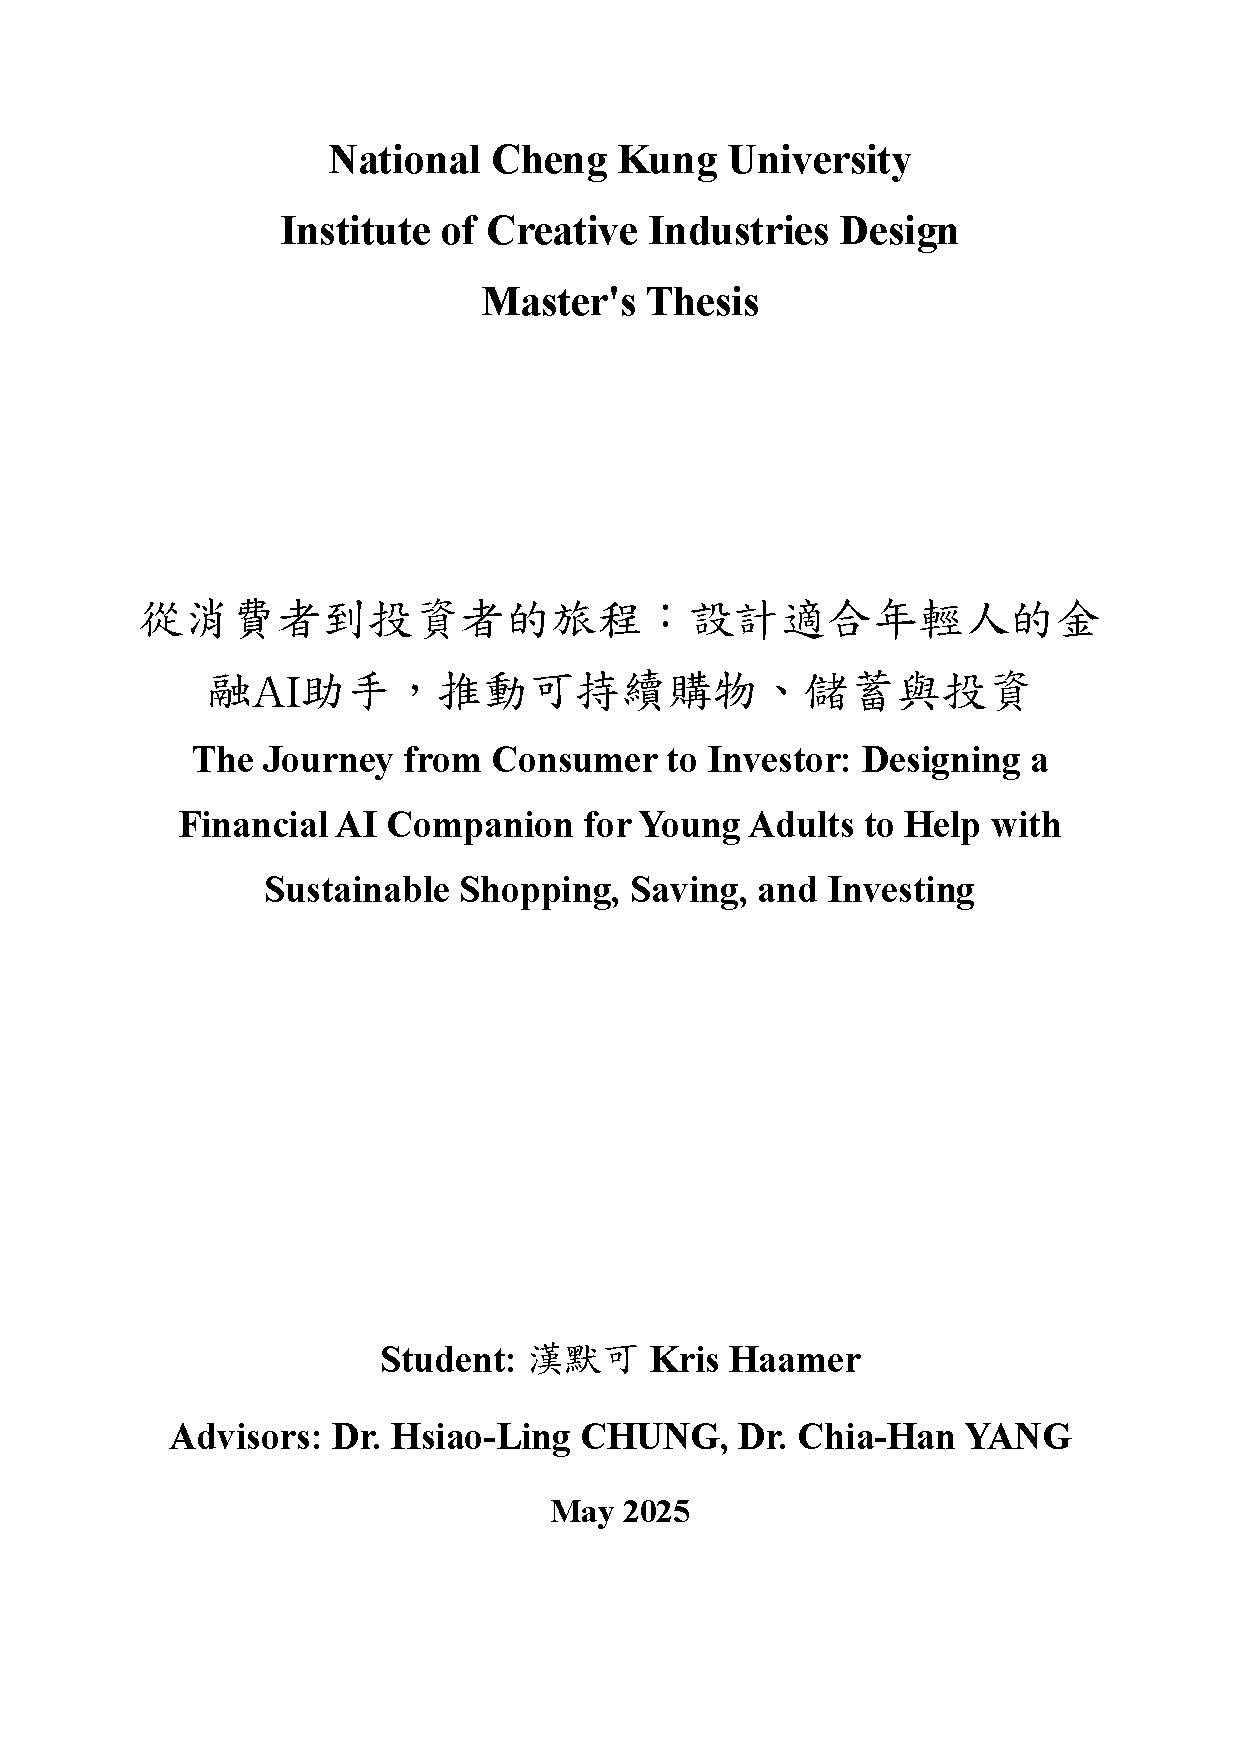
\includepdf[
  pages=1,
  fitpaper=true,
  pagecommand={\thispagestyle{empty}}
]{_cover.pages.pdf}
\clearpage

\newpage

\section{Abstract}\label{abstract}

The emerging field of \emph{Planetary Health} recognizes profound
interconnections between our economic behaviors, ecosystem services
(water, air, soil), the climate crisis, and human health. In essence,
how we use money to interact with companies - through shopping, or
saving and investing - impacts the life-supporting biosphere we depend
on. From an ecological perspective, every financial action is either an
investment to support more environmentally-friendly companies - or to
support polluters.

In Taiwan, college students genuinely care about environmental issues,
yet seen through the lens of the \emph{Theory of Planned Behaviour}
(TPB) their attitudes alone are not enough: they also need reinforcing
social norms and a sense of behavioural control. European Union
initiatives such as digital product passports (DPPs) have the potential
to supply those missing pieces, giving students a common data-driven
benchmark (norms) and arming each person with sustainability facts at
the moment of choice (control).

In my inquiry, I leveraged \emph{design research} to find design
concepts for \emph{simple AI-based generative user interfaces} to help
young adults participate in \emph{sustainable financial actions}.
Throughout the process, I conducted a survey of over 900 students from
20 universities across Taiwan, in-person user testing with 30
participants, and 7 expert interviews. The major contribution of the
study is an interactive AI-companion prototype.

Keywords: Human-AI Interaction, Digital Sustainability, Transparency

\newpage

\section{摘要}\label{ux6458ux8981}

新興的「地球健康」(Planetary
Health)領域指出,我們的經濟行為、生態系統服務(如水、空氣、土壤)、氣候危機與人類健康之間存在著深層連結。簡單來說,當我們用金錢與企業互動------無論是購物還是儲蓄與投資------都會直接影響維繫地球宜居性的生命支撐系統。從生態角度看,每一筆財務決策,不是支持更環保的企業,就是替污染者背書。

在臺灣,大學生真心關注環境議題,但依「計畫行為理論」(TPB)來看,只有態度仍不足;他們還需要被強化的社會規範,以及對行動的控制感。歐盟推出的「數位產品護照」(DPPs)等措施,可能補上這些缺口:一方面提供共同且以數據為本的基準(規範),另一方面在購買當下給予可持續性資訊(控制感)。

本研究透過設計研究方法,探索「簡易 AI
生成式使用者介面」的設計概念,以協助年輕族群參與可持續的財務行動。研究過程包含:調查來自全臺
20 所大學的 900 多名學生、對 30 位參與者進行現場使用者測試,以及 7
位專家訪談。最終成果是一個互動式 AI 夥伴原型。

關鍵詞:人機互動、數位可持續性、透明度

\emph{The abstract was translated on May 22, 2024 using the Claude 3
Opus model. Translation quality was checked with OpenAI GPT-4, Google
Gemini, Mistral Large, Meta LLama, as well as human reviewers, and
further refined with the OpenAI o1-preview model in November 2024 and
finally with o3 in July 2025. In case of any discrepancies, please refer
to the English text.}

\newpage

\section{Acknowledgments}\label{acknowledgments}

Thank you mom. Aitäh.

I'd like to express my gratitude to my entire family, 小猴子, professors
and mentors. Thank you all for your patience, help and guidance.

\newpage

\tableofcontents
\clearpage 
\listoffigures
\clearpage 
\SavedLoT

\newpage

\section{List of Symbols and
Abbreviations}\label{list-of-symbols-and-abbreviations}

Some of the key terminology used in my thesis presented in a concise
format.

\begin{enumerate}
\def\labelenumi{\arabic{enumi}.}
\item
  AI - Artificial intelligence, a field of computer science and an
  umbrella term focused on a wide range of approaches to automation
\item
  UX - User experience, a field of study and operational approach
  focused on how humans experience using systems
\item
  AX - Algorithmic experience, a proposed category of user experience,
  that is focused on interfaces between AI algorithms and humans
\item
  UI - User interface, such as in a mobile app, however increasingly
  audio, video, etc
\item
  XAI - AI user experience, interaction design applied to AI concerned
  with how does a person or a group of people interact with the AI
\item
  Fintech - Financial technology, the application of technology (usually
  AI), to classic financial services, such as payments
\item
  ESG - Environmental, Social, and Corporate Governance, a new set of
  metrics proposed by the European Union, and adopted worldwide, to
  assess business and financial assets
\item
  AI Assistant - software system providing the user with personalized
  suggestions based on machine learning algorithms
\item
  Financial Advisor - a human financial specialist providing customized
  financial advice, including investment advice and services to a client
\item
  ML - Machine learning, a tool within the larger AI umbrella to enable
  computers to learn from large sets of data, which may be labeled (by
  humans) or un-labeled (auto-labeled)
\item
  HCI - Human-computer interaction, a field of study to improve human
  experience with information technology
\item
  OEM - Original equipment manufacturer, a company making products for
  another company that markets and sells such products under their own
  brand
\item
  API - Application Programming Interface, a method for software agents
  to exchange information in various forms of data: the basis for
  contemporary online services
\item
  EPR - Extended Producer Responsibility
\item
  SDGs - Sustainable Development Goals, a set of targets agreed upon by
  the nations of the world
\item
  LLM - Large Language Models
\item
  Vector Databases - specialized data storage for mathematical language
  embeddings in multi-dimensional space helpful for clustering similar
  concepts
\item
  CO\textsubscript{2}eq - CO\textsubscript{2} equivalent greenhouse
  gases
\item
  GHG - Greenhause gases
\item
  PD - Participatory Design
\item
  VCM - Voluntary Carbon Markets
\item
  Hedge Fund - pooled investment fund
\item
  DAO - Decentralized Autonomous Organization
\item
  Zero Waste - according to Zero Waste International Alliance:
  \emph{``conservation of all resources by means of responsible
  production, consumption, reuse and recovery of products, packaging and
  materials without burning, and with no discharges to land, water or
  air that threaten the environment or human health''} - (Kalle et al.,
  2022)
\item
  ESPR - Ecodesign for Sustainable Products Regulation
\item
  NFRD - Non-Financial Reporting Directive
\item
  CSRD - Corporate Sustainability Reporting Directive
\item
  EUDR - European Union Deforestation Regulation
\item
  Product Stewardship
\item
  Extended Producer Responsibility
\end{enumerate}

\newpage

\section{Introduction}\label{introduction}

How can college students find sustainable companies? Furthermore, if
given appropriate tools, could college students leverage their
purchasing power to reward sustainable companies? Why is this important
to research now? Young people should invest in their future and younger
generations like services with a green, eco-conscious focus. Given our
combined power (I'm a Millennial) with Generation Z, we are willing to
pay more for sustainable products. Does Individual Climate Action
Matter?

My research describes the process of designing an AI companion for
college students to help with sustainable shopping, saving, and
investing. Money spent shopping, saving, and investing in sustainable
companies serves as an incentive to adopt more sustainable practices. If
used wisely, money can reward companies for becoming more sustainable.
Encourage the least sustainable companies to improve their performance,
raising the overall baseline. Facilitate the formation of communities
centered around environmental stewardship. Build closer relationships
with sustainability.

\begin{figure}[H]

{\centering 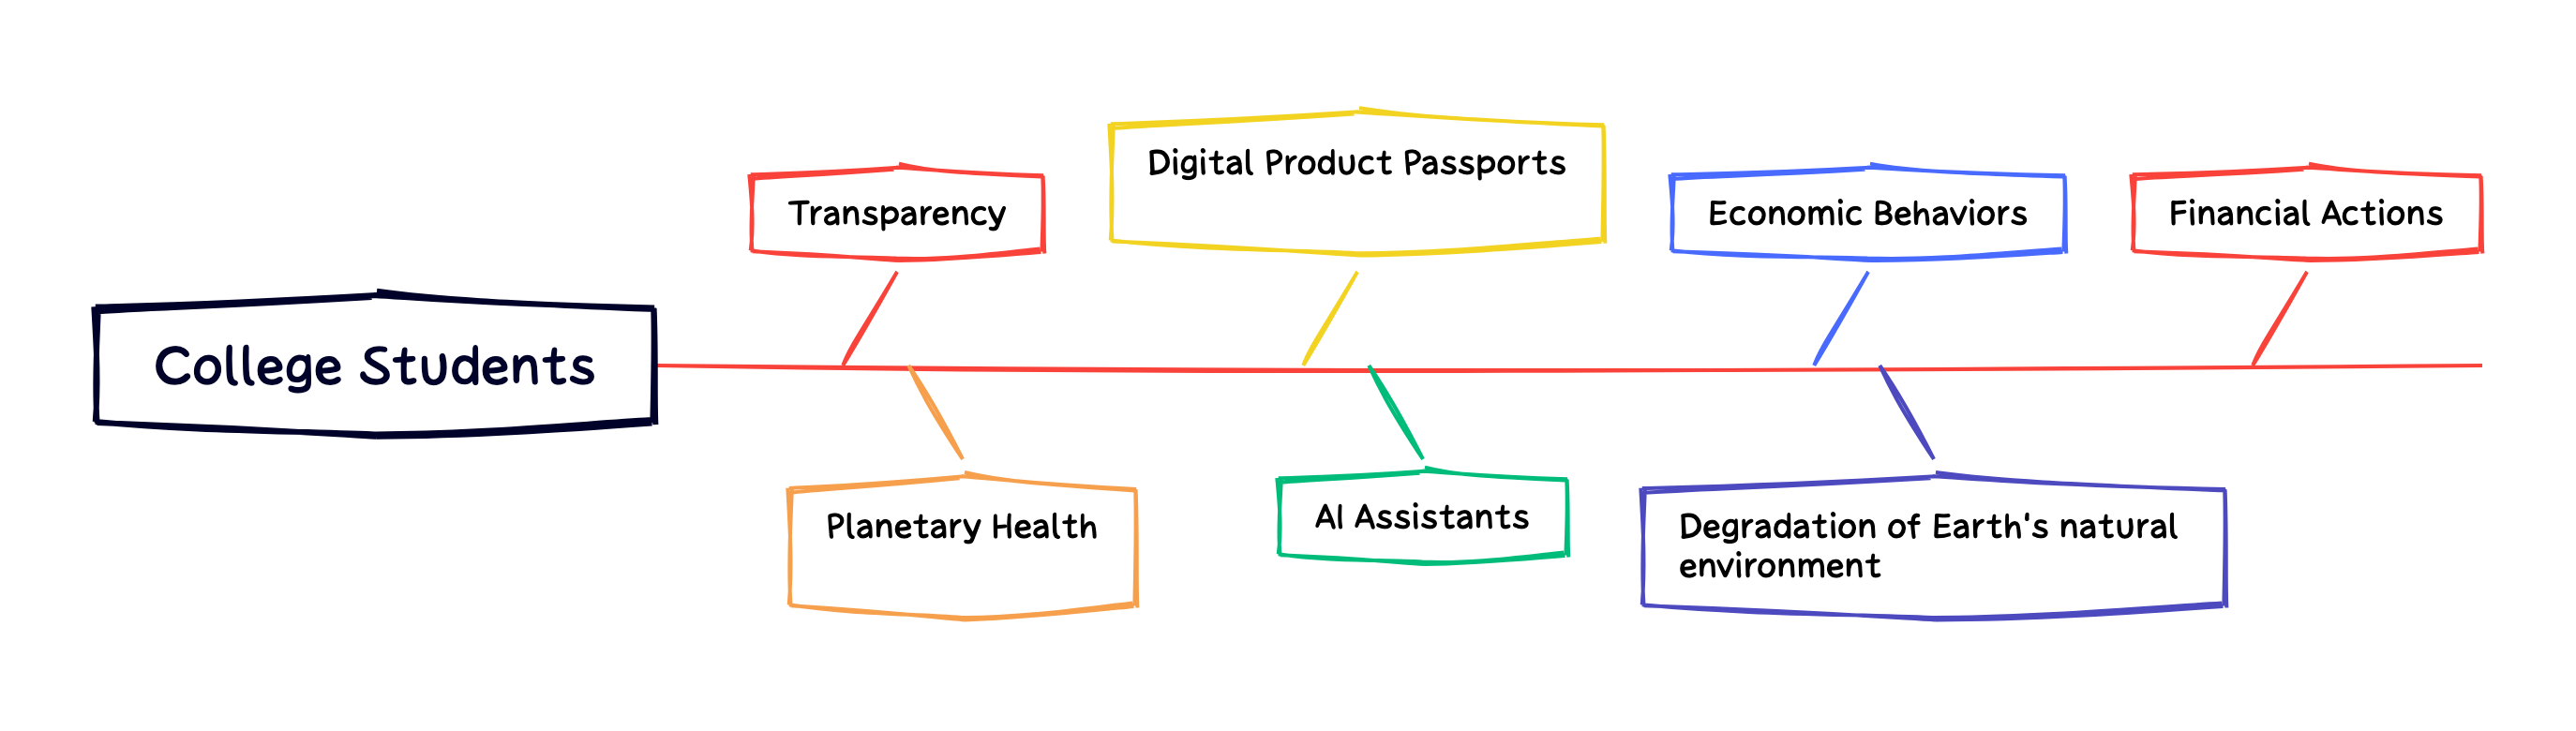
\includegraphics[width=1\linewidth,height=\textheight,keepaspectratio]{./images/introduction/abstract.png}

}

\caption{College Students}

\end{figure}%

\subsection{Relevance and Research
Gap}\label{relevance-and-research-gap}

My research addresses the \emph{``attitude-behavior gap''} among
Taiwanese college students in taking sustainable financial action. In
general, Icek Ajzen's \emph{Theory of Planned Behavior} frames the gap
between attitude and behavior by showing that (1) attitude, (2)
perceived social norms, and (3) perceived control, must all converge,
before intention can translate into any action (Ajzen, 1991) - in this
case, taking sustainable financial action.

In terms of the global context, the convergence of the following 5
trends makes my research timely in 2025.

\begin{longtable}[]{@{}
  >{\raggedright\arraybackslash}p{(\linewidth - 2\tabcolsep) * \real{0.4167}}
  >{\raggedright\arraybackslash}p{(\linewidth - 2\tabcolsep) * \real{0.5833}}@{}}
\caption{Trending global narratives.}\tabularnewline
\toprule\noalign{}
\begin{minipage}[b]{\linewidth}\raggedright
Trend
\end{minipage} & \begin{minipage}[b]{\linewidth}\raggedright
Direction
\end{minipage} \\
\midrule\noalign{}
\endfirsthead
\toprule\noalign{}
\begin{minipage}[b]{\linewidth}\raggedright
Trend
\end{minipage} & \begin{minipage}[b]{\linewidth}\raggedright
Direction
\end{minipage} \\
\midrule\noalign{}
\endhead
\bottomrule\noalign{}
\endlastfoot
Environmental degradation & Worsening \\
Interest in sustainability among young people & ? \\
Intergenerational money transfer; in some countries relatively young
people have money & ? \\
Availability of sustainability tools such as ESG, B Corporations, Green
Bonds, etc, among metrics and instruments & Increasing \\
Availability of generative AI-based user interfaces (UIs) &
Increasing \\
Democratization of Financial Markets & Increasing \\
\end{longtable}

\subsection{Background}\label{background}

I grew up as an avid science fiction reader, which influenced my outlook
towards future possibilities. In particular, the Star Trek universe had
an imaginary portable device called a \textbf{\emph{tricorder}} (fig.~1)
enabling scientists to scan anything for insights. Be it precious
minerals inside a cave or scanning the human bodies for medical data,
its sensors would show up with some useful data. In daily life, I would
love to have such a device for consumer choices and financial decisions
- to know what to buy and which businesses to support with my money and
approval.

\begin{figure}

\centering{


\includegraphics[width=0.5\linewidth,height=\textheight,keepaspectratio]{./images/introduction/tricorder.jpg}

}

\caption{\label{fig-co2-tricorder}Captain Sulu using a Tricorder (Star
Trek) - Photo copyright by Paramount Pictures}

\end{figure}%

While a \emph{tricorder} is still science fiction, technological
advancements are getting closer and closer to producing something
similar. AIs are already integral to many parts of our lives, with
computer models producing increasingly useful outputs. The proposal for
this thesis was first written using Google's and Apple's voice
recognition software in 2020, and later switching to OpenAI's
\emph{Whisper} model, allowing me to transcribe notes with the help of
an AI assistant. As a foreigner living in Taiwan since 2019, I relied on
AI-based tools for many aspects of my life: speaking, moving, finding
food and services. When writing in Chinese, Apple's text prediction
algorithms translate pinyin to 漢字 and show the most likely character
based on my previous writing, Google's maps find efficient and
eco-friendly routes and recommend places to eat and ChatGPT provides
statistically probable advice from the sum of human knowledge. Even when
we don't realize it, AI is helping us with many mundane tasks. While it
takes incredibly complex computational algorithms to achieve all this in
the background, it's become so commonplace, we don't even think about
it. From this point of view, another AI assistant to help students with
choosing more eco-friendly businesses - to shop, save, and invest -
doesn't sound so much of a stretch.

\subsection{Motivation}\label{motivation}

Environmental degradation is increasingly affecting human lives - and
it's largely driven by manufacturing processes - of the products we
consume daily. From resource extraction in the linear economy (mining
raw materials and drilling for fossil fuels) to chemical processes
(causing contamination and pollution of the air, water, and soil) to
waste generation and greenhouse gas emissions, industries transform the
natural world into consumer products. While industry practices have
improved since the industrial revolution in the 19th century, and
continue to improve, it's possible to further improve standards of
production and raise the global baseline for sustainability, given
enough societal pressure to do so.

Nonetheless, without easily accessible and reliable data, it's difficult
to know which company is more sustainable than another. As consumers and
investors (even if only through passive ownership of savings), we don't
really know much about enterprise production practices, unless we spend
a lot of time looking at the numbers, which may be costly to access (for
example ESG reports are expensive), and mostly rely on our governments
and international bodies to keep us safe. Or just look at the brands
themselves - and pick the ones which we like.

\subsection{Objective}\label{objective}

The study presents design research for developing an AI companion to
help college students find sustainable companies for shopping, saving
and investing. The major contribution of my study is an interactive
artefact (a prototype) informed by design research.

\subsection{Demographics}\label{demographics}

The research focuses on young adults, specifically Taiwanese college
students studying in Taiwan.

\begin{longtable}[]{@{}ll@{}}
\toprule\noalign{}
Criteria & \\
\midrule\noalign{}
\endhead
\bottomrule\noalign{}
\endlastfoot
Location & Taiwan \\
Population & College Students \\
Count & 900 \\
\end{longtable}

Experts (finance, design, sustainability).

\begin{longtable}[]{@{}ll@{}}
\toprule\noalign{}
Criteria & \\
\midrule\noalign{}
\endhead
\bottomrule\noalign{}
\endlastfoot
Location & Global \\
Population & Experts \\
Count & 7 \\
\end{longtable}

\subsection{Research Questions}\label{research-questions}

My research attempts to answer the following questions.

\begin{longtable}[]{@{}
  >{\raggedright\arraybackslash}p{(\linewidth - 2\tabcolsep) * \real{0.5556}}
  >{\raggedright\arraybackslash}p{(\linewidth - 2\tabcolsep) * \real{0.4444}}@{}}
\caption{Research Questions}\tabularnewline
\toprule\noalign{}
\begin{minipage}[b]{\linewidth}\raggedright
Question
\end{minipage} & \begin{minipage}[b]{\linewidth}\raggedright
Methods
\end{minipage} \\
\midrule\noalign{}
\endfirsthead
\toprule\noalign{}
\begin{minipage}[b]{\linewidth}\raggedright
Question
\end{minipage} & \begin{minipage}[b]{\linewidth}\raggedright
Methods
\end{minipage} \\
\midrule\noalign{}
\endhead
\bottomrule\noalign{}
\endlastfoot
What design considerations should be addressed when designing an AI
companion for college students integrating sustainability and finance? &
Literature Review and Expert Interviews \\
How can AI companions support college students with sustainability
knowledge in the context of financial decisions? & Literature Review,
Expert Interviews and Survey of College Students \\
What AI companion features do college students prioritize as the
highest? & Survey of College Students and Prototype Testing \\
\end{longtable}

\subsubsection{Why These Research
Questions?}\label{why-these-research-questions}

\begin{longtable}[]{@{}
  >{\raggedright\arraybackslash}p{(\linewidth - 6\tabcolsep) * \real{0.2192}}
  >{\raggedright\arraybackslash}p{(\linewidth - 6\tabcolsep) * \real{0.2603}}
  >{\raggedright\arraybackslash}p{(\linewidth - 6\tabcolsep) * \real{0.3014}}
  >{\raggedright\arraybackslash}p{(\linewidth - 6\tabcolsep) * \real{0.2192}}@{}}
\toprule\noalign{}
\begin{minipage}[b]{\linewidth}\raggedright
Lens
\end{minipage} & \begin{minipage}[b]{\linewidth}\raggedright
\textbf{RQ1}: Design Considerations
\end{minipage} & \begin{minipage}[b]{\linewidth}\raggedright
\textbf{RQ2:} Support Mechanisms
\end{minipage} & \begin{minipage}[b]{\linewidth}\raggedright
\textbf{RQ3}: User-Priority Features
\end{minipage} \\
\midrule\noalign{}
\endhead
\bottomrule\noalign{}
\endlastfoot
Level of Abstraction & High-level and comprehensive & Mid-level
(mechanisms) & Concrete and granular \\
Core Focus & \emph{What should I keep in mind while building?} &
\emph{How does the companion actually help students learn and decide?} &
\emph{Which specific features matter most to students?} \\
Primary Stakeholder & Designers / Developers & End Users (College
Students) & End Users (College Students) \\
Outputs & Design guidelines, UX principles, tech constraints, ethical
guardrails & Framework of nudges, learning aids, information flows. &
Ranked feature list, must-have vs nice-to-have. \\
Data Sources & Literature Review and Expert Interviews & Literature
Review, Expert Interviews and Survey of College Students & Survey of
College Students and Prototype Testing \\
\end{longtable}

\newpage

\section{Methodology}\label{methodology}

\subsection{Research Design}\label{research-design}

(Baytaş, 2020) categorizes design research into three modes: (1)
conducting research to inform design decisions, (2) studying designs to
generate knowledge, and (3) using design itself as a means of inquiry.
My research is of the 1st category, aiming to make better design
decisions for my sustainability-focused financial app. When developing
my research design, I relied on the advice of (Christian Rohrer, 2022)
to decide when to choose which user experience research methods.

To knit together the themes of youth finance and sustainability, with
the help of interaction design and AI, this study adopts the
\emph{Theory of Planned Behavior} (TPB) as its primary analytic frame
used to organize the overall results from a theoretical point of view.
TPB states that the strength of a person's intention depends on three
belief clusters: (1) a cognitive and affective attitude toward the act,
(2) perceived social norms, and (3) perceived behavioral control (Ajzen,
1991).

By foregrounding TPB I can interpret both the adoption of a financial AI
companion and the subsequent shift toward sustainable shopping, saving,
and investing with a single set of constructs. (Hagger \& Hamilton,
2025) extensive meta-meta-study (study of several underlying
meta-studies) summarize 40 years of TPB research, showing strong,
consistent effects of \emph{attitude}, \emph{subjective norm}, and
\emph{perceived behavioral control} on \emph{intentions}, and of
intentions on behavior; the effect is found to be robust across various
behaviors, populations, and study designs.

The graph below shows the basic structure of TPB.

\begin{figure}

\centering{

\pandocbounded{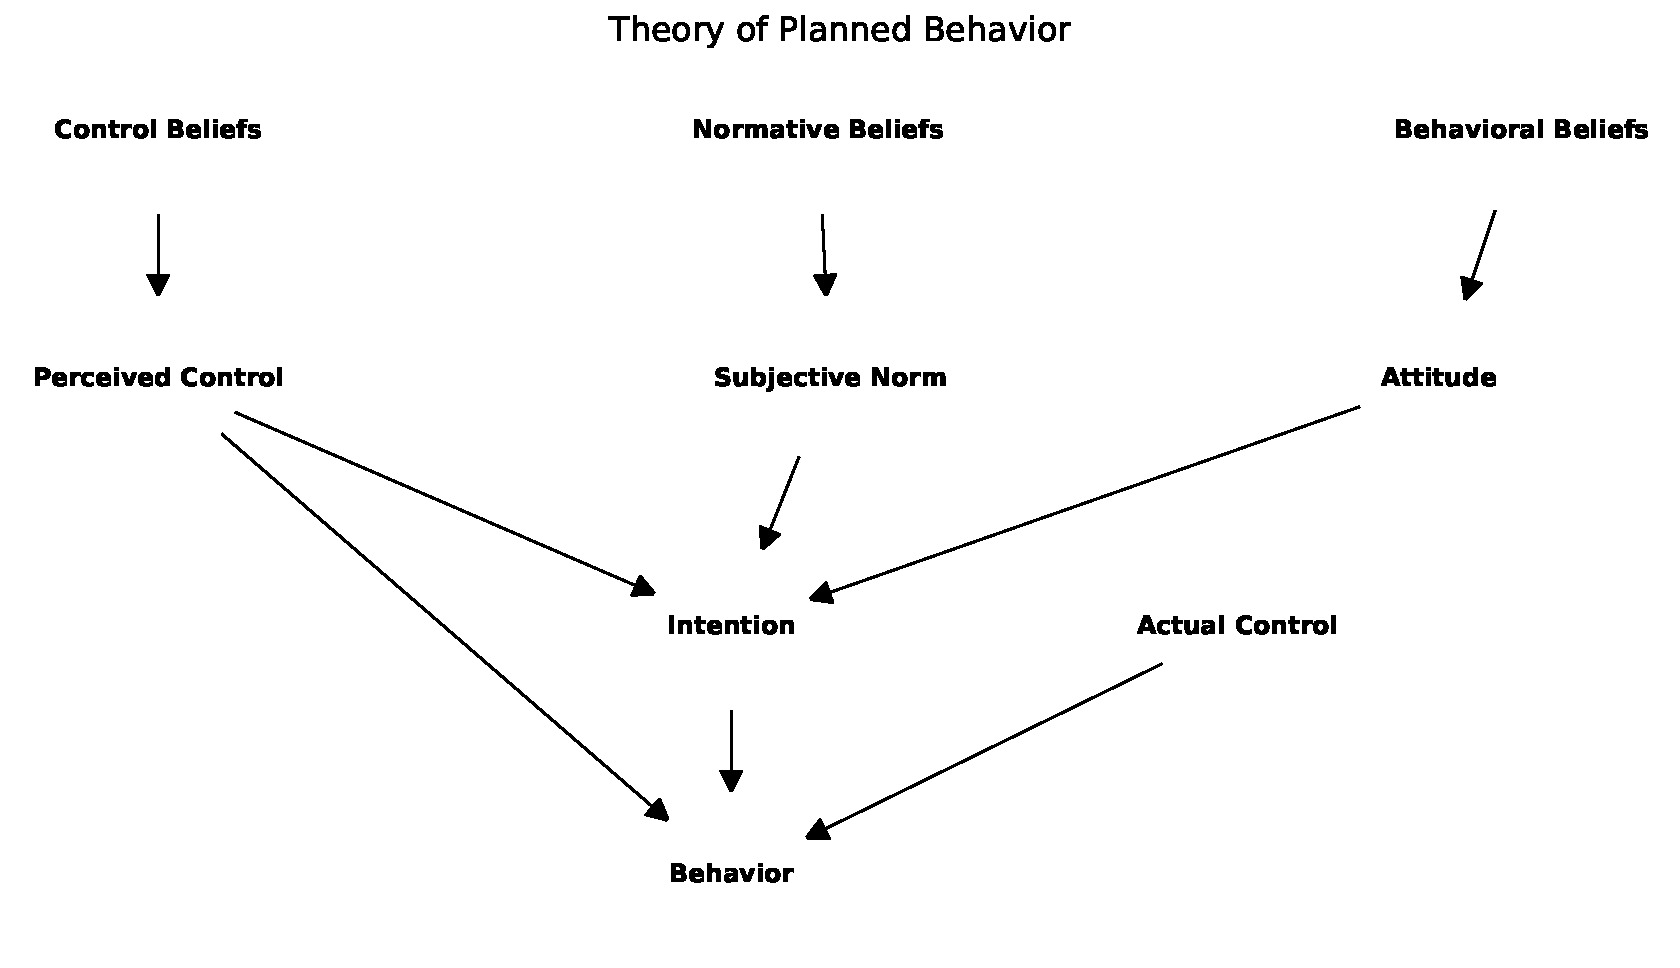
\includegraphics[keepaspectratio]{_thesis-nocite_files/figure-pdf/fig-plan-beh-output-1.pdf}}

}

\caption[Theory of Planned Behaviour]{\label{fig-plan-beh}Theory of
Planned Behaviour}

\end{figure}%

Additional theoretical lenses used in my work include the following.

\begin{longtable}[]{@{}
  >{\raggedright\arraybackslash}p{(\linewidth - 4\tabcolsep) * \real{0.2400}}
  >{\raggedright\arraybackslash}p{(\linewidth - 4\tabcolsep) * \real{0.3733}}
  >{\raggedright\arraybackslash}p{(\linewidth - 4\tabcolsep) * \real{0.3867}}@{}}
\caption{Theoretical lenses found in my research.}\tabularnewline
\toprule\noalign{}
\begin{minipage}[b]{\linewidth}\raggedright
Theory / Framework
\end{minipage} & \begin{minipage}[b]{\linewidth}\raggedright
Key Contribution
\end{minipage} & \begin{minipage}[b]{\linewidth}\raggedright
Sections Where Used
\end{minipage} \\
\midrule\noalign{}
\endfirsthead
\toprule\noalign{}
\begin{minipage}[b]{\linewidth}\raggedright
Theory / Framework
\end{minipage} & \begin{minipage}[b]{\linewidth}\raggedright
Key Contribution
\end{minipage} & \begin{minipage}[b]{\linewidth}\raggedright
Sections Where Used
\end{minipage} \\
\midrule\noalign{}
\endhead
\bottomrule\noalign{}
\endlastfoot
Theory of Planned Behaviour (TPB) & Core explanatory model linking
attitudes, norms, control and intention to sustainable finance behaviour
& Overall \\
Planetary Boundaries & Situates individual financial choices within
global ecological thresholds & Sustainability \\
Circular Economy & Provides closed-loop design principles for
product-passport features & Design / Money \\
Triple Bottom Line (TBL) & Connects profit, people and planet in ESG
analysis & Money \\
Technology Acceptance Model (TAM) & Explains perceived usefulness / ease
of use for AI companion & AI \\
Fogg Behaviour Model (FBM) & Maps motivation-ability-trigger nudges in
UI & Design \\
Heuristic--Systematic Model (HSM) & Explains quick credibility
heuristics vs.~deep cues & AI \\
Algorithmic Experience (AX) model & Describes how users form mental
models of opaque AI & AI \\
Choice Architecture / Behavioural Nudges & Frames defaults and
eco-filter prompts in super-app context & Design \\
Systems Thinking & Positions app interventions within broader
supply-chain loops & Design \\
Ecological \& Doughnut Economics & Critiques GDP-only metrics; motivates
regenerative finance lens & Money \\
Participatory / Multi-species Design & Broadens stakeholder set to
non-human actors & Design \\
Service Design for Sustainability & Maps end-to-end user journey
(repair, swap, delivery) & Design \\
Earth-System Law & Links micro-level nudges to macro-level legal
frameworks & Sustainability \\
\end{longtable}

\subsection{Research Methods}\label{research-methods}

Overview of research methods.

\begin{longtable}[]{@{}ll@{}}
\toprule\noalign{}
Group & Task \\
\midrule\noalign{}
\endhead
\bottomrule\noalign{}
\endlastfoot
Experts (Finance) & Interview \\
Experts (Design) & Interview \\
Experts (Sustainability) & Interview \\
Target Audience (College Students) & Survey \\
Target Audience (College Students) & Prototype Testing \\
\end{longtable}

This mixed-method research design is divided into three stages.

\subsubsection{Phase One - Qualitative
Research}\label{phase-one---qualitative-research}

My purpose for the first qualitative stage is to explore the general
themes arising from the literature review related to the design of AI
advisors for investing. I identified specific user experience factors,
through interviewing experts in financial technology and user experience
design and reviewing existing applications on the marketplace. At this
stage in the research, the central concept being studied was defined
generally as expectations towards a sustainable investment AI advisor.

I started with literature review, which led into expert interviews
(there were many questions arising from the literature). I identified
key concepts from expert discussions and gained exposure to their
industry insights.

The qualitative research methods employed in the first stage of the
research design enables me to explore concepts arising for literature
review further, using a more open approach, without limiting the
conversation only to pre-ascribed notions. The strength of the
qualitative approach in the first stage is to encourage the discovery of
new ideas, not yet common in literature and potential user experience
factors related to sustainable investing and user experience.

\paragraph{Sampling}\label{sampling}

My qualitative sampling structure used non-probability snowball
sampling, with the following criteria: targeting financial industry,
fintech, design, and sustainability experts; located everywhere.

\paragraph{Methods}\label{methods}

I conducted exploratory research in English using semi-structured
interviews recorded online and offline. I talked to 5 experts over video
call, 1 expert face-to-face, and 1 expert over WhatsApp voice messages;
6 interviews were conducted in English and 1 in Portuguese. I recorded
audio and video, transcribed the conversations. I used OpenAI's o3 model
to translate the Portuguese interview to English. I then performed
thematic analysis across all the contents, leading to a \emph{wish list}
of features.

\begin{longtable}[]{@{}
  >{\raggedright\arraybackslash}p{(\linewidth - 6\tabcolsep) * \real{0.3000}}
  >{\raggedright\arraybackslash}p{(\linewidth - 6\tabcolsep) * \real{0.2714}}
  >{\raggedright\arraybackslash}p{(\linewidth - 6\tabcolsep) * \real{0.1714}}
  >{\raggedright\arraybackslash}p{(\linewidth - 6\tabcolsep) * \real{0.2571}}@{}}
\toprule\noalign{}
\begin{minipage}[b]{\linewidth}\raggedright
Interview Mode
\end{minipage} & \begin{minipage}[b]{\linewidth}\raggedright
Number of Experts
\end{minipage} & \begin{minipage}[b]{\linewidth}\raggedright
Language
\end{minipage} & \begin{minipage}[b]{\linewidth}\raggedright
Recording Method
\end{minipage} \\
\midrule\noalign{}
\endhead
\bottomrule\noalign{}
\endlastfoot
Video Call & 5 & English & Audio \& Video \\
Face-to-Face & 1 & English & Audio \& Video \\
WhatsApp Voice Msgs & 1 & Portuguese & Audio \\
\end{longtable}

Thematic analysis coding was developed using Atlas.ti ``Intentional AI
Coding'' feature, using the following prompt:

\begin{quote}
``How do industry experts describe their design and sustainability
principles, AI and technology strategies? What common language emerges
between design, sustainability, finance, and AI? Identify passages where
experts link system thinking, transparency, simplicity, feedback loops,
and long term impact across design, sustainability, AI, and finance.'' -
Prompt for Atlas.ti ``Intentional AI Coding''
\end{quote}

Specific questions generated by Atlast.ti from the prompt, which guide
the AI coding.

\begin{longtable}[]{@{}
  >{\raggedright\arraybackslash}p{(\linewidth - 2\tabcolsep) * \real{0.7917}}
  >{\raggedright\arraybackslash}p{(\linewidth - 2\tabcolsep) * \real{0.2083}}@{}}
\toprule\noalign{}
\begin{minipage}[b]{\linewidth}\raggedright
Question
\end{minipage} & \begin{minipage}[b]{\linewidth}\raggedright
Category
\end{minipage} \\
\midrule\noalign{}
\endhead
\bottomrule\noalign{}
\endlastfoot
How do industry experts describe their design and sustainability
principles? & Design Principles \\
What AI and technology strategies do industry experts employ? & AI
Strategies \\
What common language emerges between design, sustainability, finance,
and AI? & Common Language \\
How do experts link systems thinking across design, sustainability, AI,
and finance? & System Thinking \\
In what ways do experts emphasize transparency in their discussions on
design, sustainability, AI, and finance? & Transparency \\
How is simplicity articulated by experts in relation to design,
sustainability, AI, and finance? & Simplicity \\
What role do feedback loops play in the experts' frameworks for design,
sustainability, AI, and finance? & Feedback Loops \\
How do experts define long term impact in the context of design,
sustainability, AI, and finance? & Long term Impact \\
\end{longtable}

\paragraph{Conceptual Framework}\label{conceptual-framework}

The conceptual framework map presents the key concepts arising from the
literature review thus far in the research process. I'm using these
concepts when developing interview strategies for phase one of the
research, developing the survey questionnaire for phase two, as well as
for building the Green Filter AI Companion for young adults at the final
stage of the process. However, I expect the conceptual framework to
further evolve with additional findings while conducting my research.

\begin{figure}[H]

{\centering 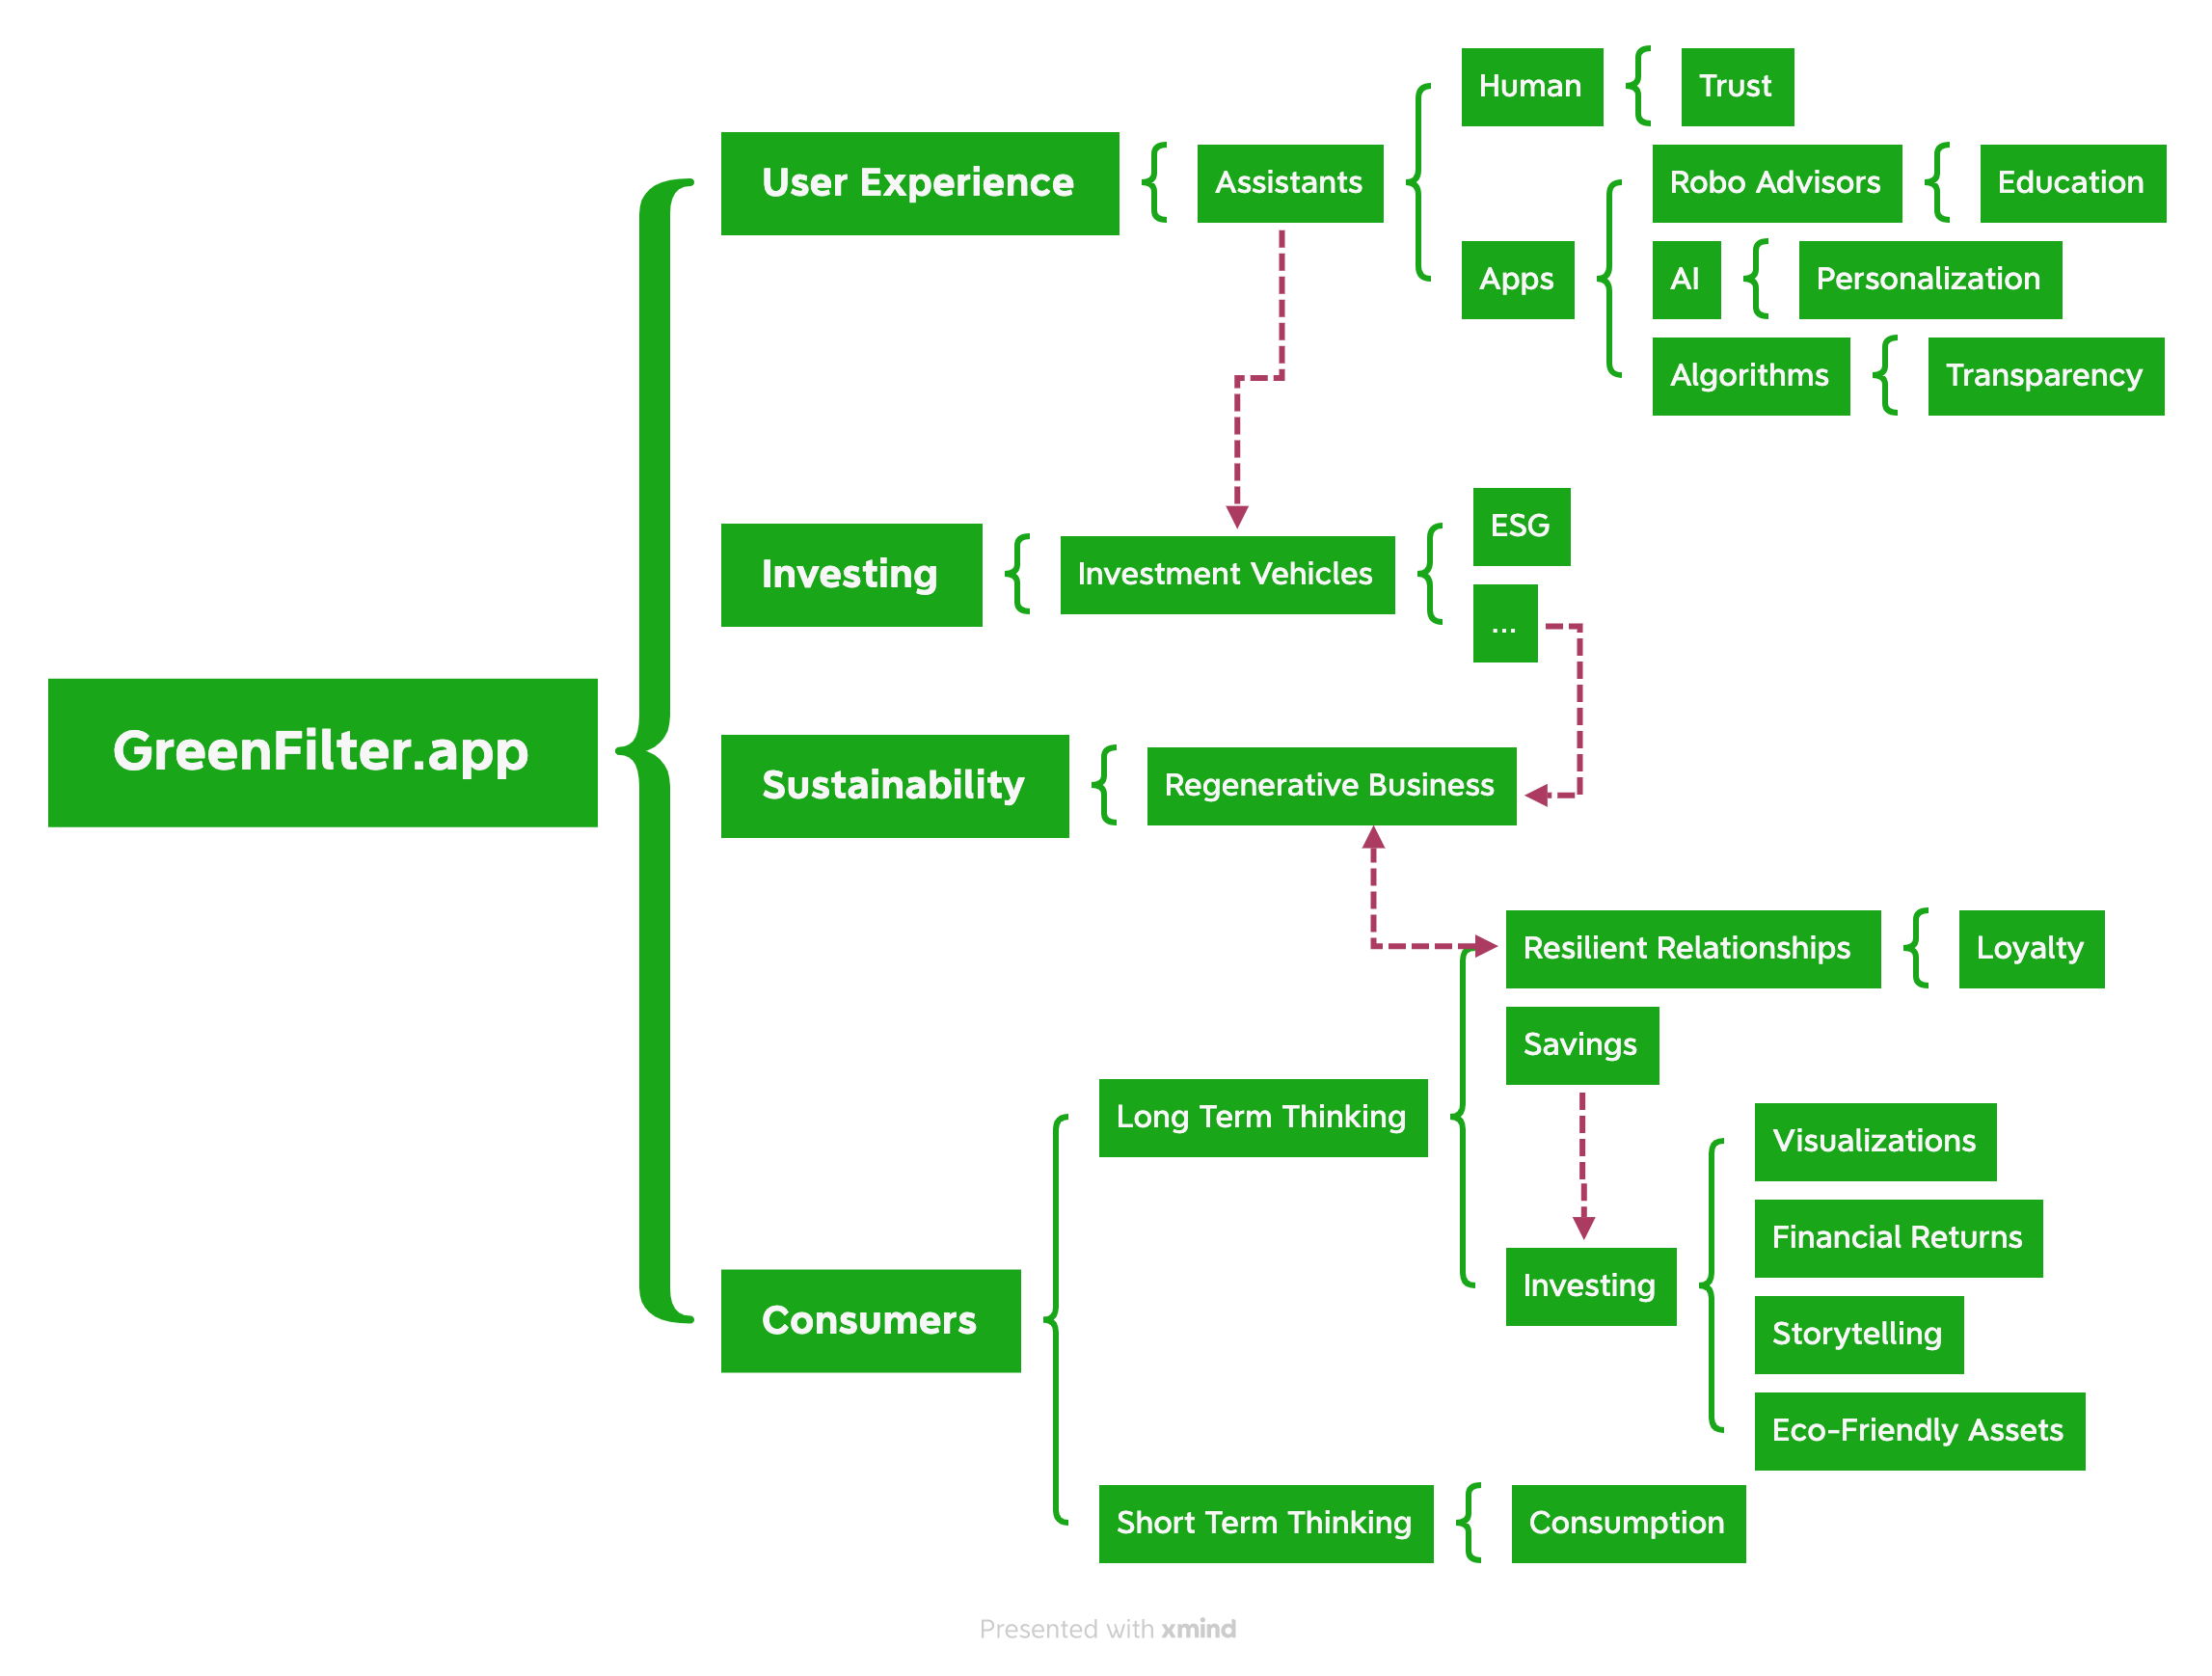
\includegraphics[width=1\linewidth,height=\textheight,keepaspectratio]{./images/methodology/concept-map.png}

}

\caption{Concept map}

\end{figure}%

Conceptual Model

Initial version of the concept map focused on the app itself.

Current concept map focusing on sustainability:

\begin{figure}[H]

{\centering 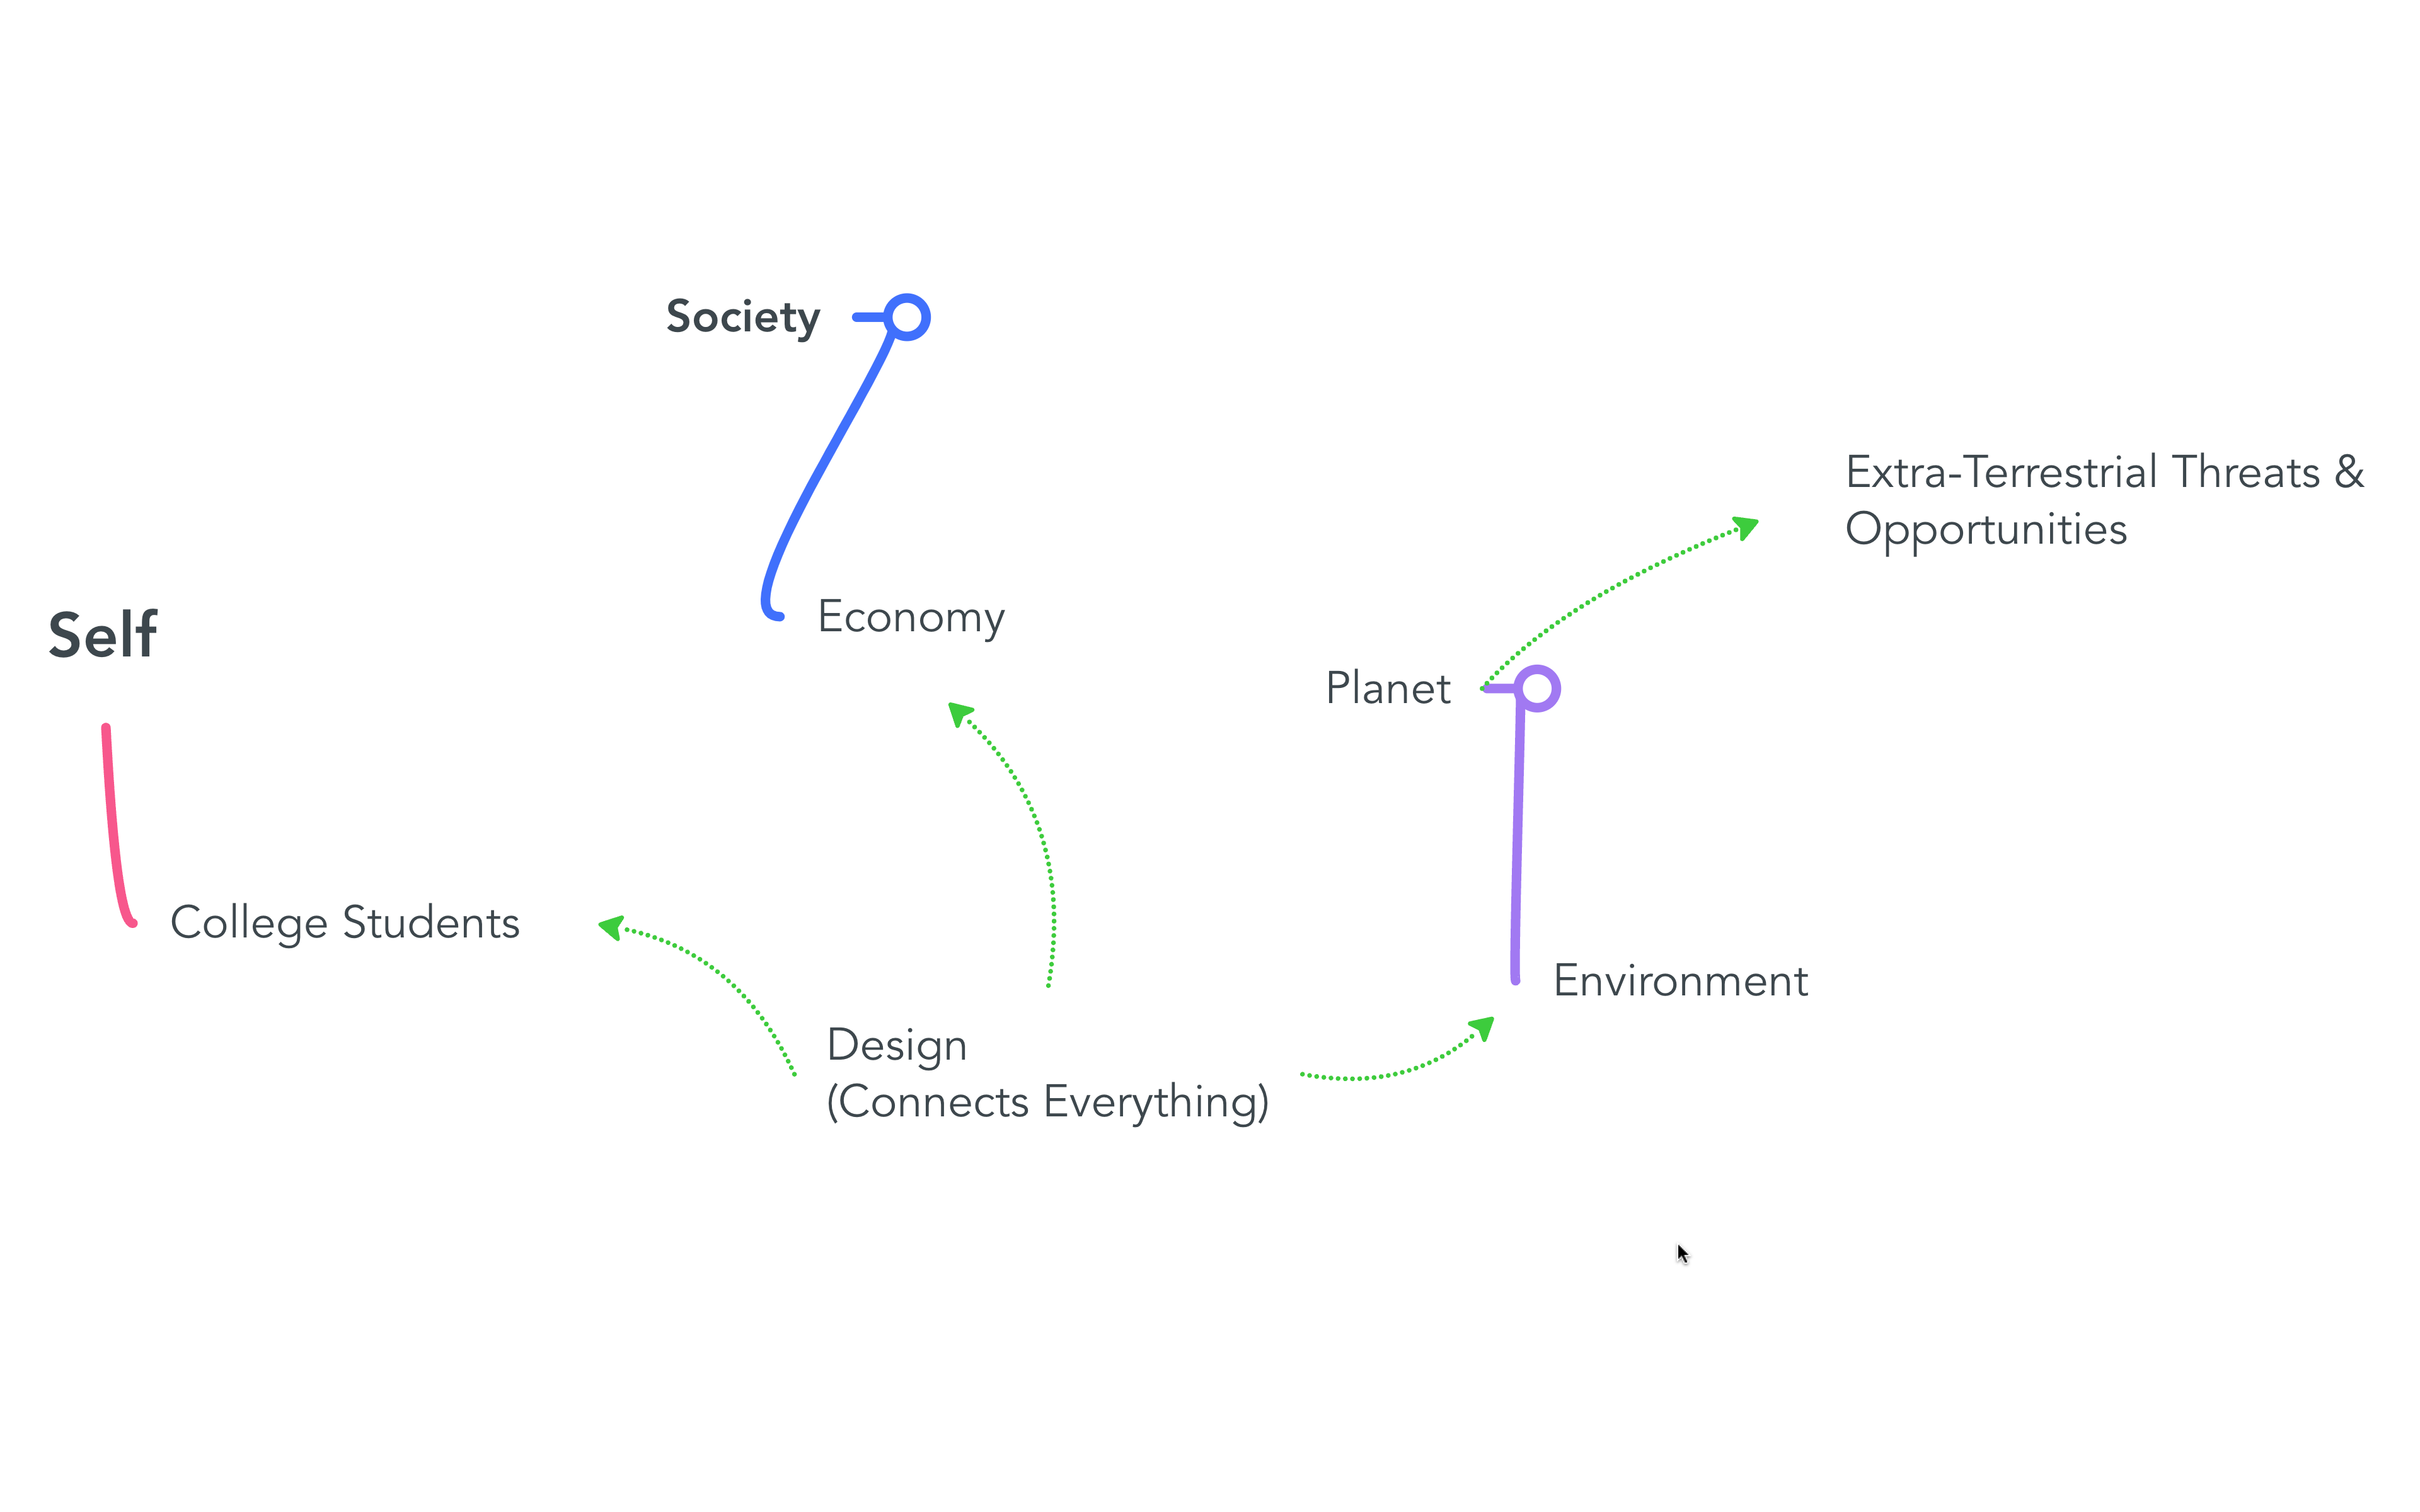
\includegraphics[width=1\linewidth,height=\textheight,keepaspectratio]{./images/discussion/everything.png}

}

\caption{Overall Concept Map}

\end{figure}%

\subsubsection{Phase Two - Quantitative
Research}\label{phase-two---quantitative-research}

I then proceeded to the second, quantitative stage, informed by the
previously identified factors, and prepared a survey to understand
potential users' preferences, including a Likert scale, a choice
experiment, and a selection of proposed features, focusing on the
preferences of the potential users in Gen-Z, aged 18-29, living in
Taiwan.

\paragraph{Sampling}\label{sampling-1}

My quantitative sampling structure uses a judgmental criterion: adults
aged in Gen-Z (18-29), located in Taiwan, surveyed using a
Chinese-language online survey.

\paragraph{Methods}\label{methods-1}

Likert: The survey includes a Likert scale between 1 to 5 to validate
key findings from the first stage of the research by assessing responses
to statements regarding the app's design, features, and other criteria
that may still emerge.

Choice Experiment: The survey includes a \emph{choice experiment}
between different sets of potential features available when
communicating with the sustainable finance AI companion.

\paragraph{Survey Development and Expected
Findings}\label{survey-development-and-expected-findings}

In December 2020, in preparation for the final version of the survey, I
ran a preliminary questionnaire, testing open-ended and close-ended
questions, as way to prepare for the proposal of this research. I
conducted a preliminary round of face-to-face interviews using 21
open-ended, probing questions and a convenience sampling of NCKU foreign
students (n = 12) on campus between ages 19 and 29. The interviews were
conducted in English and lasted between 9 and 21 minutes; they gave me
some initial feedback on my research idea, the respondents' daily
routines, app usage, and feelings towards financial questions, including
investing, relationship with nature, and environmental sustainability

This preliminary version of the survey was only used to develop the
questionnaire itself and the data collected (even though the recorded
audio was transcribed), is not part of the research results. These
preliminary conversations led me to emphasize more on the financial
journey of the user, i.e.~to consider the importance of the shopping,
savings, and payments, with the apps students already use daily, serving
as an entry point to becoming an investor (this approach later became
known as embedded finance). I expected my future research findings to
confirm this initial idea and to offer diverse ways and examples of what
that path could look like in practice.

I then proceeded to change my target audience to Taiwanese students and
developed the survey to include more specific questions, including more
close-ended multiple-choice varieties.

\paragraph{Final Survey: Data
Collection}\label{final-survey-data-collection}

For the actual survey, I developed 63 close-ended and open-ended
questions. For survey distribution, I adopted a face-to-face method to
increase response rates, distributing flyers to students on college
campuses, canteens, and classrooms, getting verbal permission from
educators in their classrooms to distribute the survey flyer. Similarly
to the approach take by (C.-H. Liu et al., 2023), I distributed the
survey flyer at universities located in the Northern, Soutern, Central,
and East regions of Taiwan. The flyer included a colorful AI-generated
visual with a futuristic game-like female figure, and the title
``climate anxiety survey'' in Chinese, as well as a website link
(ziran.tw) and scannable QR-code.

The survey only included questions and descriptions in Chinese. I have
used the Claude 3 Opus model to translate them to English for this
table.

\begin{longtable}[]{@{}
  >{\raggedright\arraybackslash}p{(\linewidth - 2\tabcolsep) * \real{0.4722}}
  >{\raggedright\arraybackslash}p{(\linewidth - 2\tabcolsep) * \real{0.5278}}@{}}
\caption{36 Likert Fields included in the survey}\tabularnewline
\toprule\noalign{}
\begin{minipage}[b]{\linewidth}\raggedright
Original Question in Chinese
\end{minipage} & \begin{minipage}[b]{\linewidth}\raggedright
English Translation
\end{minipage} \\
\midrule\noalign{}
\endfirsthead
\toprule\noalign{}
\begin{minipage}[b]{\linewidth}\raggedright
Original Question in Chinese
\end{minipage} & \begin{minipage}[b]{\linewidth}\raggedright
English Translation
\end{minipage} \\
\midrule\noalign{}
\endhead
\bottomrule\noalign{}
\endlastfoot
如果你/妳懷疑你/妳要買的番茄可能是由強迫勞工(現代奴隸)採摘的,你/妳仍然會買它嗎?
& If you suspect that the tomatoes you are going to buy may have been
picked by forced labor (modern slaves), would you still buy them? \\
你/妳關心食安嗎? & Do you care about food safety? \\
你/妳7年內買車嗎?🚘 & Will you buy a car within 7 years? 🚘 \\
你/妳7年內買房嗎?🏡 & Will you buy a house within 7 years? 🏡 \\
你/妳購物時知道產品環保嗎? & Do you know if the products are
environmentally friendly when you shop? \\
你/妳覺得認證環保的公司更好嗎? & Do you think companies certified as
environmentally friendly are better? \\
你/妳支持肉稅嗎? & Do you support a meat tax? \\
你/妳關心食用雞的生活嗎? & Do you care about the lives of chickens
raised for food? \\
你/妳避免吃肉嗎? & Do you avoid eating meat? \\
你/妳覺得你/妳花錢會影響環境嗎? & Do you think your spending affects
the environment? \\
你/妳會對金錢感到焦慮嗎? & Do you feel anxious about money? \\
你/妳會對金錢很節儉嗎? & Are you very frugal with money? \\
你/妳會經常存錢嗎? & Do you often save money? \\
你/妳對自己的財務知識滿意嗎? & Are you satisfied with your financial
knowledge? \\
你/妳投資會考慮環保嗎? & Do you consider environmental protection when
investing? \\
你/妳覺得台灣的經濟目標是增長嗎? & Do you think Taiwan's economic goal
is growth? \\
你/妳覺台灣的得環境退化是台灣的經濟增長的前提嗎? & Do you think
environmental degradation in Taiwan is a prerequisite for Taiwan's
economic growth? \\
你/妳覺得台灣的經濟增長有助於保護環境嗎? & Do you think Taiwan's
economic growth helps protect the environment? \\
你/妳覺得經濟能不排CO\textsubscript{2}eq也增長嗎? & Do you think the
economy can grow without emitting CO\textsubscript{2}eq? \\
你/妳覺得經濟增長有物質限制嗎? & Do you think there are material limits
to economic growth? \\
你/妳會每天都用AI嗎? & Do you use AI every day? \\
你/妳會信任AI嗎? & Do you trust AI? \\
你/妳想要AI有個造型嗎? & Do you want AI to have a specific
appearance? \\
你/妳喜歡待在大自然嗎? & Do you like being in nature? \\
你/妳擔心氣候變化嗎? & Are you worried about climate change? \\
你/妳對環境污染情況會感到焦慮嗎? & Do you feel anxious about
environmental pollution? \\
你/妳知道許多植物和動物的名字嗎? & Do you know the names of many plants
and animals? \\
你/妳感覺自己和大自然很接近嗎? & Do you feel close to nature? \\
你/妳努力實踐低碳生活嗎? & Do you strive to live a low-carbon
lifestyle? \\
你/妳想做更多環保事嗎? & Do you want to do more for environmental
protection? \\
你/妳對環境相關政治議題有興趣嗎? & Are you interested in environmental
political issues? \\
你/妳信任碳排放抵消額度嗎? & Do you trust carbon offset credits? \\
你/妳的環保行動對環境保護有效果嗎? & Do your environmental actions have
an effect on environmental protection? \\
你/妳想在行業內推環保嗎? & Do you want to promote environmental
protection within your industry? \\
你/妳得自己對新觀念開放嗎? & Are you open to new ideas? \\
你/妳的大學對可環保性支持嗎? & Does your university support
environmental sustainability? \\
\end{longtable}

Respondents who remained outside the survey parameters were allowed to
answer the survey however their responses were disregarded from the data
analysis. References were stored in the Zotero paid version with 6 GB
storage. Bibtex and Better Bibtex were used to export the references to
the .bib format consumable by the Quarto scientific writing system.

\subsubsection{Phase Three - Qualitative
Research}\label{phase-three---qualitative-research}

In the third and last phase, I returned to qualitative methods, to
further validate the quantitative findings from stage two, by building a
prototype of the sustainable investing AI companion, taking into account
insights gathered in the previous stage. Here my focus was on
operationalizing the gathered insights into a prototype that users can
experiment with. I designed and refined a prototype of the personal
sustainable finance AI assistant. I used face-to-face interviews to
discuss the prototype, and conducted a thematic analysis of the
discussions' recordings, leading to further validation of previously
gathered data and changes in the prototype. The gained insights,
accompanied by the app prototype, which embodies my findings, are the
final outcome of my research.

\paragraph{Sampling}\label{sampling-2}

The phase three sampling structure used a judgmental criterion:

\begin{itemize}
\tightlist
\item
  Age Gen-Z cohort
\item
  Located in Taiwan
\item
  Using Chinese for discussion.
\end{itemize}

Individual face-to-face interviews were organized at universities around
Taiwan. Because in-person presence is required in this stage, the
prototype will only be tested by potential users physically present in
Taiwan. To avoid convenience sampling, I posted online ads in Chinese
and reach out to varied student clubs to invite people who I don't know
personally, to participate in a ``sustainable AI application testing''
(wording may change).

\paragraph{Methods}\label{methods-2}

Face-to-face prototype testing. The strength of in-person is the ability
to observe potential users, where knowledge can be exchanged directly.
The interviews were recorded and transcribed. Finally, I performed a
thematic analysis of the interview transcriptions in order to validate
previous findings, and open avenues for future research.

\begin{figure}[H]

{\centering 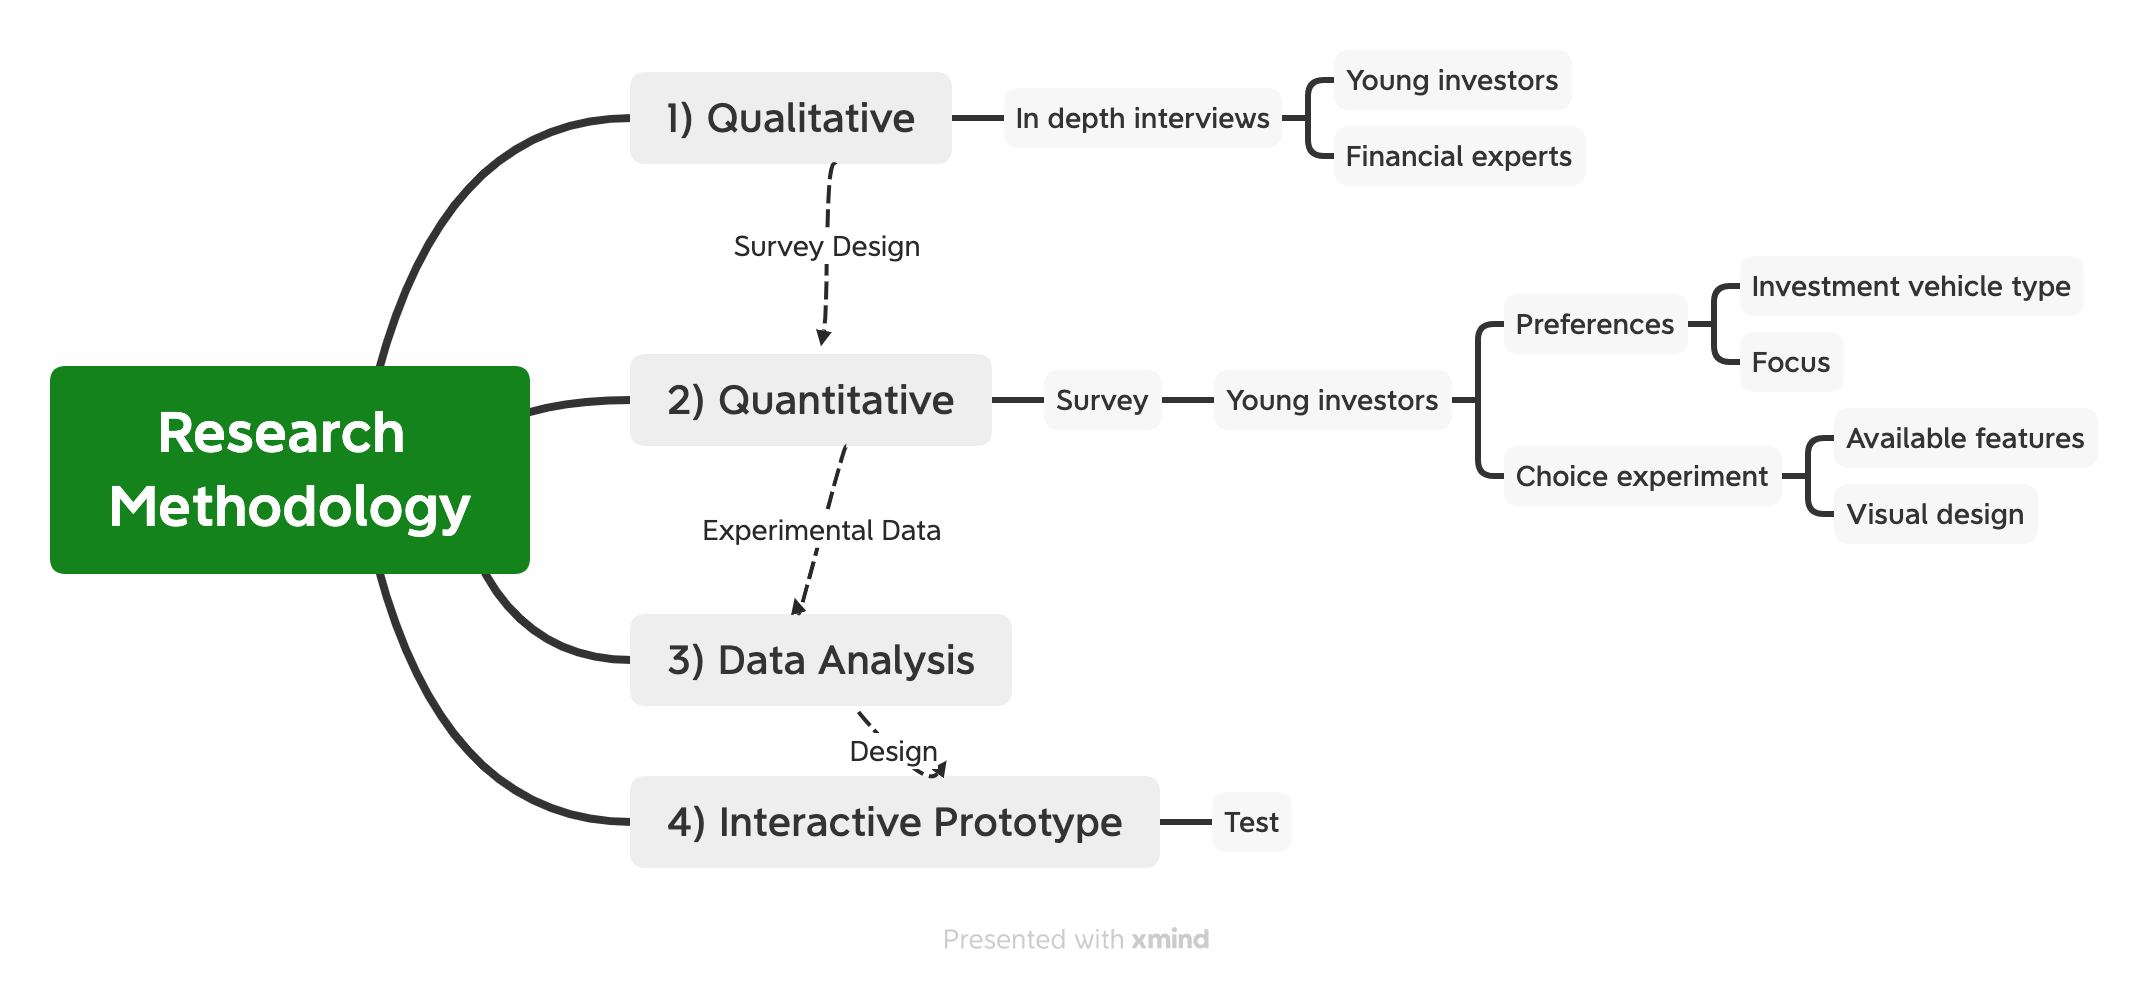
\includegraphics[width=1\linewidth,height=\textheight,keepaspectratio]{./images/methodology/research-methodology.png}

}

\caption{Overview of research methodology}

\end{figure}%

Interview transcripts from Descript and Google Speech-to-Text model were
combined using Gemini 2.5 Pro Experimental 03-25
(gemini-2.5-pro-exp-03-25) model.

\paragraph{Prototype Testing}\label{prototype-testing}

Does the prototype match user needs?

Testing was the most difficult part of the thesis process.

\begin{itemize}
\item
  Testing with random people found at the university.
\item
  Testing with experts.
\item
  Testing with unknown people in the target audience.
\end{itemize}

App Testing Flow

\begin{figure}[H]

{\centering 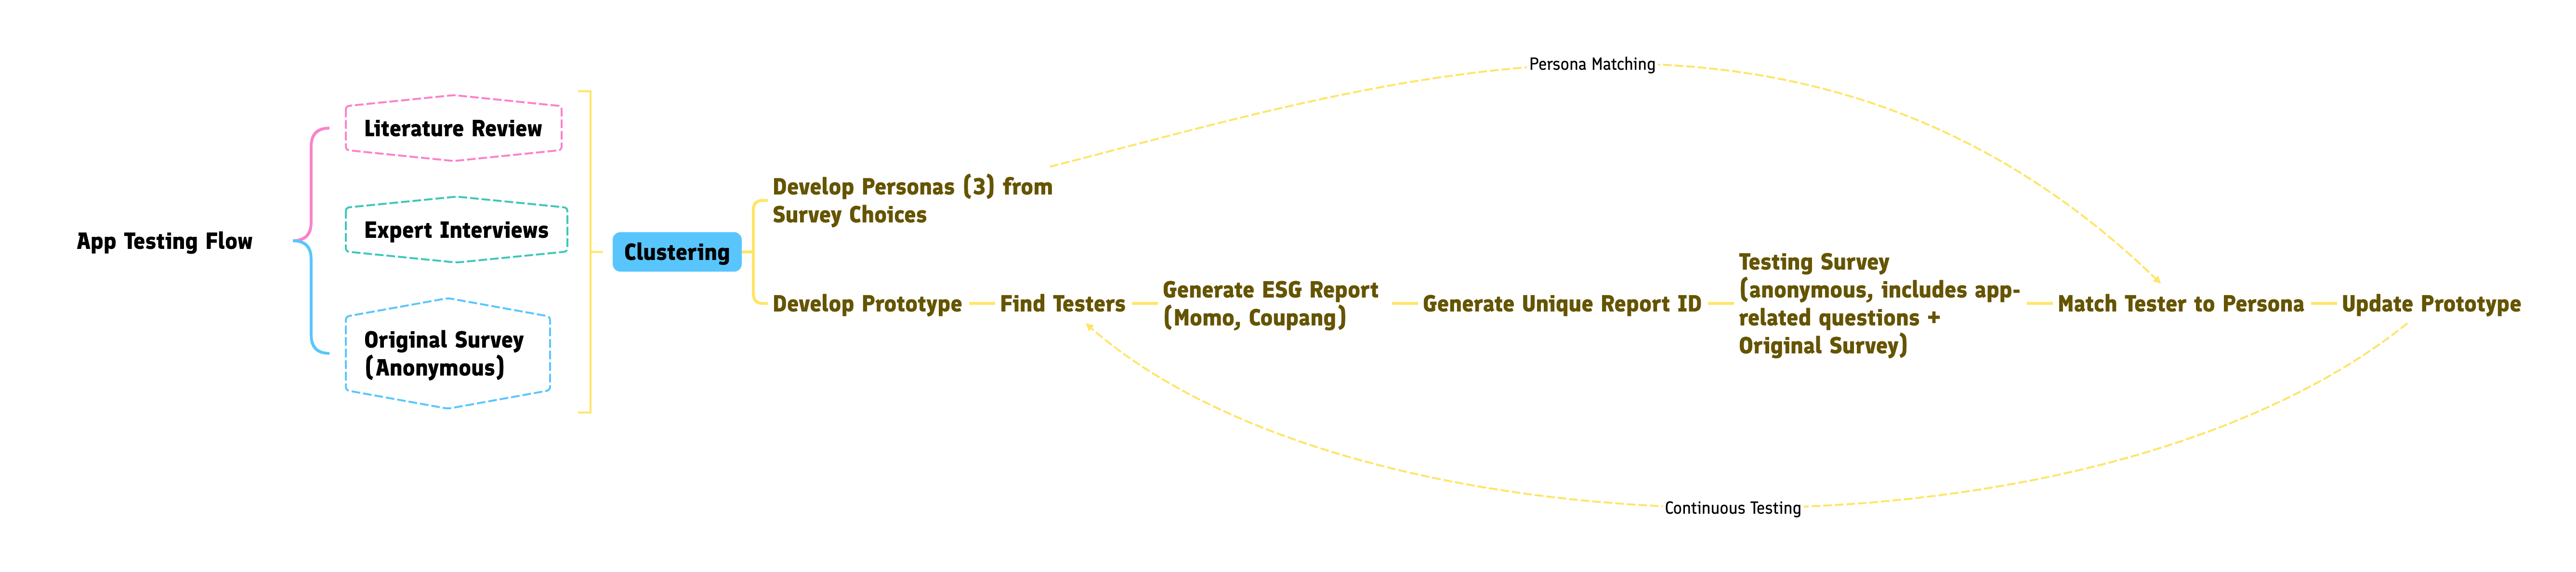
\includegraphics[width=1\linewidth,height=\textheight,keepaspectratio]{./images/testing/app-testing-flow.png}

}

\caption{App Testing Flow}

\end{figure}%

\paragraph{1st Wave of (Preliminary) Prototype Testing (Spring
2024)}\label{st-wave-of-preliminary-prototype-testing-spring-2024}

The 1st wave of preliminary testing took place during 1 month from 2024
April 2 to May 2, 2024 at the NCKU campus. I found 8 anonymous
participants at different NCKU locations, such as the student canteens
and the medical library, confirmed the people I approached were
Taiwanese students studying at NCKU, and then simply asked them to test
my app, using my own laptop. I made use of \emph{participant
observation} and took notes myself. There was no audio or video
recording.

\paragraph{2nd Wave of (In Production) Prototype Testing (Autumn 2024 -
Spring
2025)}\label{nd-wave-of-in-production-prototype-testing-autumn-2024---spring-2025}

The 2nd wave of testing took place from Autumn 2024 to Spring 2025 and
was more comprehensive. I conducted in-person face-to-face testing
individually with 32 students at 7 universities. Interviews were
conducted in Chinese and transcribed and translated to English using
Google Voice to Text AI as well as Describe AI.

\begin{longtable}[]{@{}
  >{\raggedright\arraybackslash}p{(\linewidth - 4\tabcolsep) * \real{0.2603}}
  >{\raggedright\arraybackslash}p{(\linewidth - 4\tabcolsep) * \real{0.3699}}
  >{\raggedright\arraybackslash}p{(\linewidth - 4\tabcolsep) * \real{0.3699}}@{}}
\toprule\noalign{}
\endhead
\bottomrule\noalign{}
\endlastfoot
Region & University & No of Testees \\
Taichung & 國立中興大學 National Chung Hsing University (NCHU) & 7 \\
Chiayi & 國立中正大學 National Chung Cheng University (CCU) & 5 \\
Tainan & 國立成功大學 National Cheng Kung University (NCKU) & 6 \\
Tainan & 國立臺南藝術大學 Tainan National University of the Arts (TNNUA)
& 2 \\
Tainan & 長榮大學 Chang Jung Christian University (CJCU) & 5 \\
Tainan & 南臺科技大學 Southern Taiwan University of Science and
Technology (STUST) & 5 \\
Pingtung & 國立屏東科技大學 National Pingtung University of Science and
Technology (NPUST) & 2 \\
\end{longtable}

\newpage

\subsection{Literature Review}\label{literature-review}

The literature review branches out to 5 main directions and maps out
relationships sources and the literature map, namely Taiwanese college
students, generation-z demographics, sustainability, ecology, ecosystem
services, EU legislation, sustainable finance, sustainable investing,
savings, circular economy, economics, AI, existing sustainability,
software, sustainability--related mobile apps (Apple iOS / Google
Android), and web apps related to sustainable shopping, savings, and
investing; apps using algorithmic interfaces (AI-based UI), design,
UX/UI, service design, sustainable design, speculative design,
interaction design, behavior change, nudge.

The following chart shows a tiny portion of the papers considered in
this research.

\begin{figure}[H]

{\centering 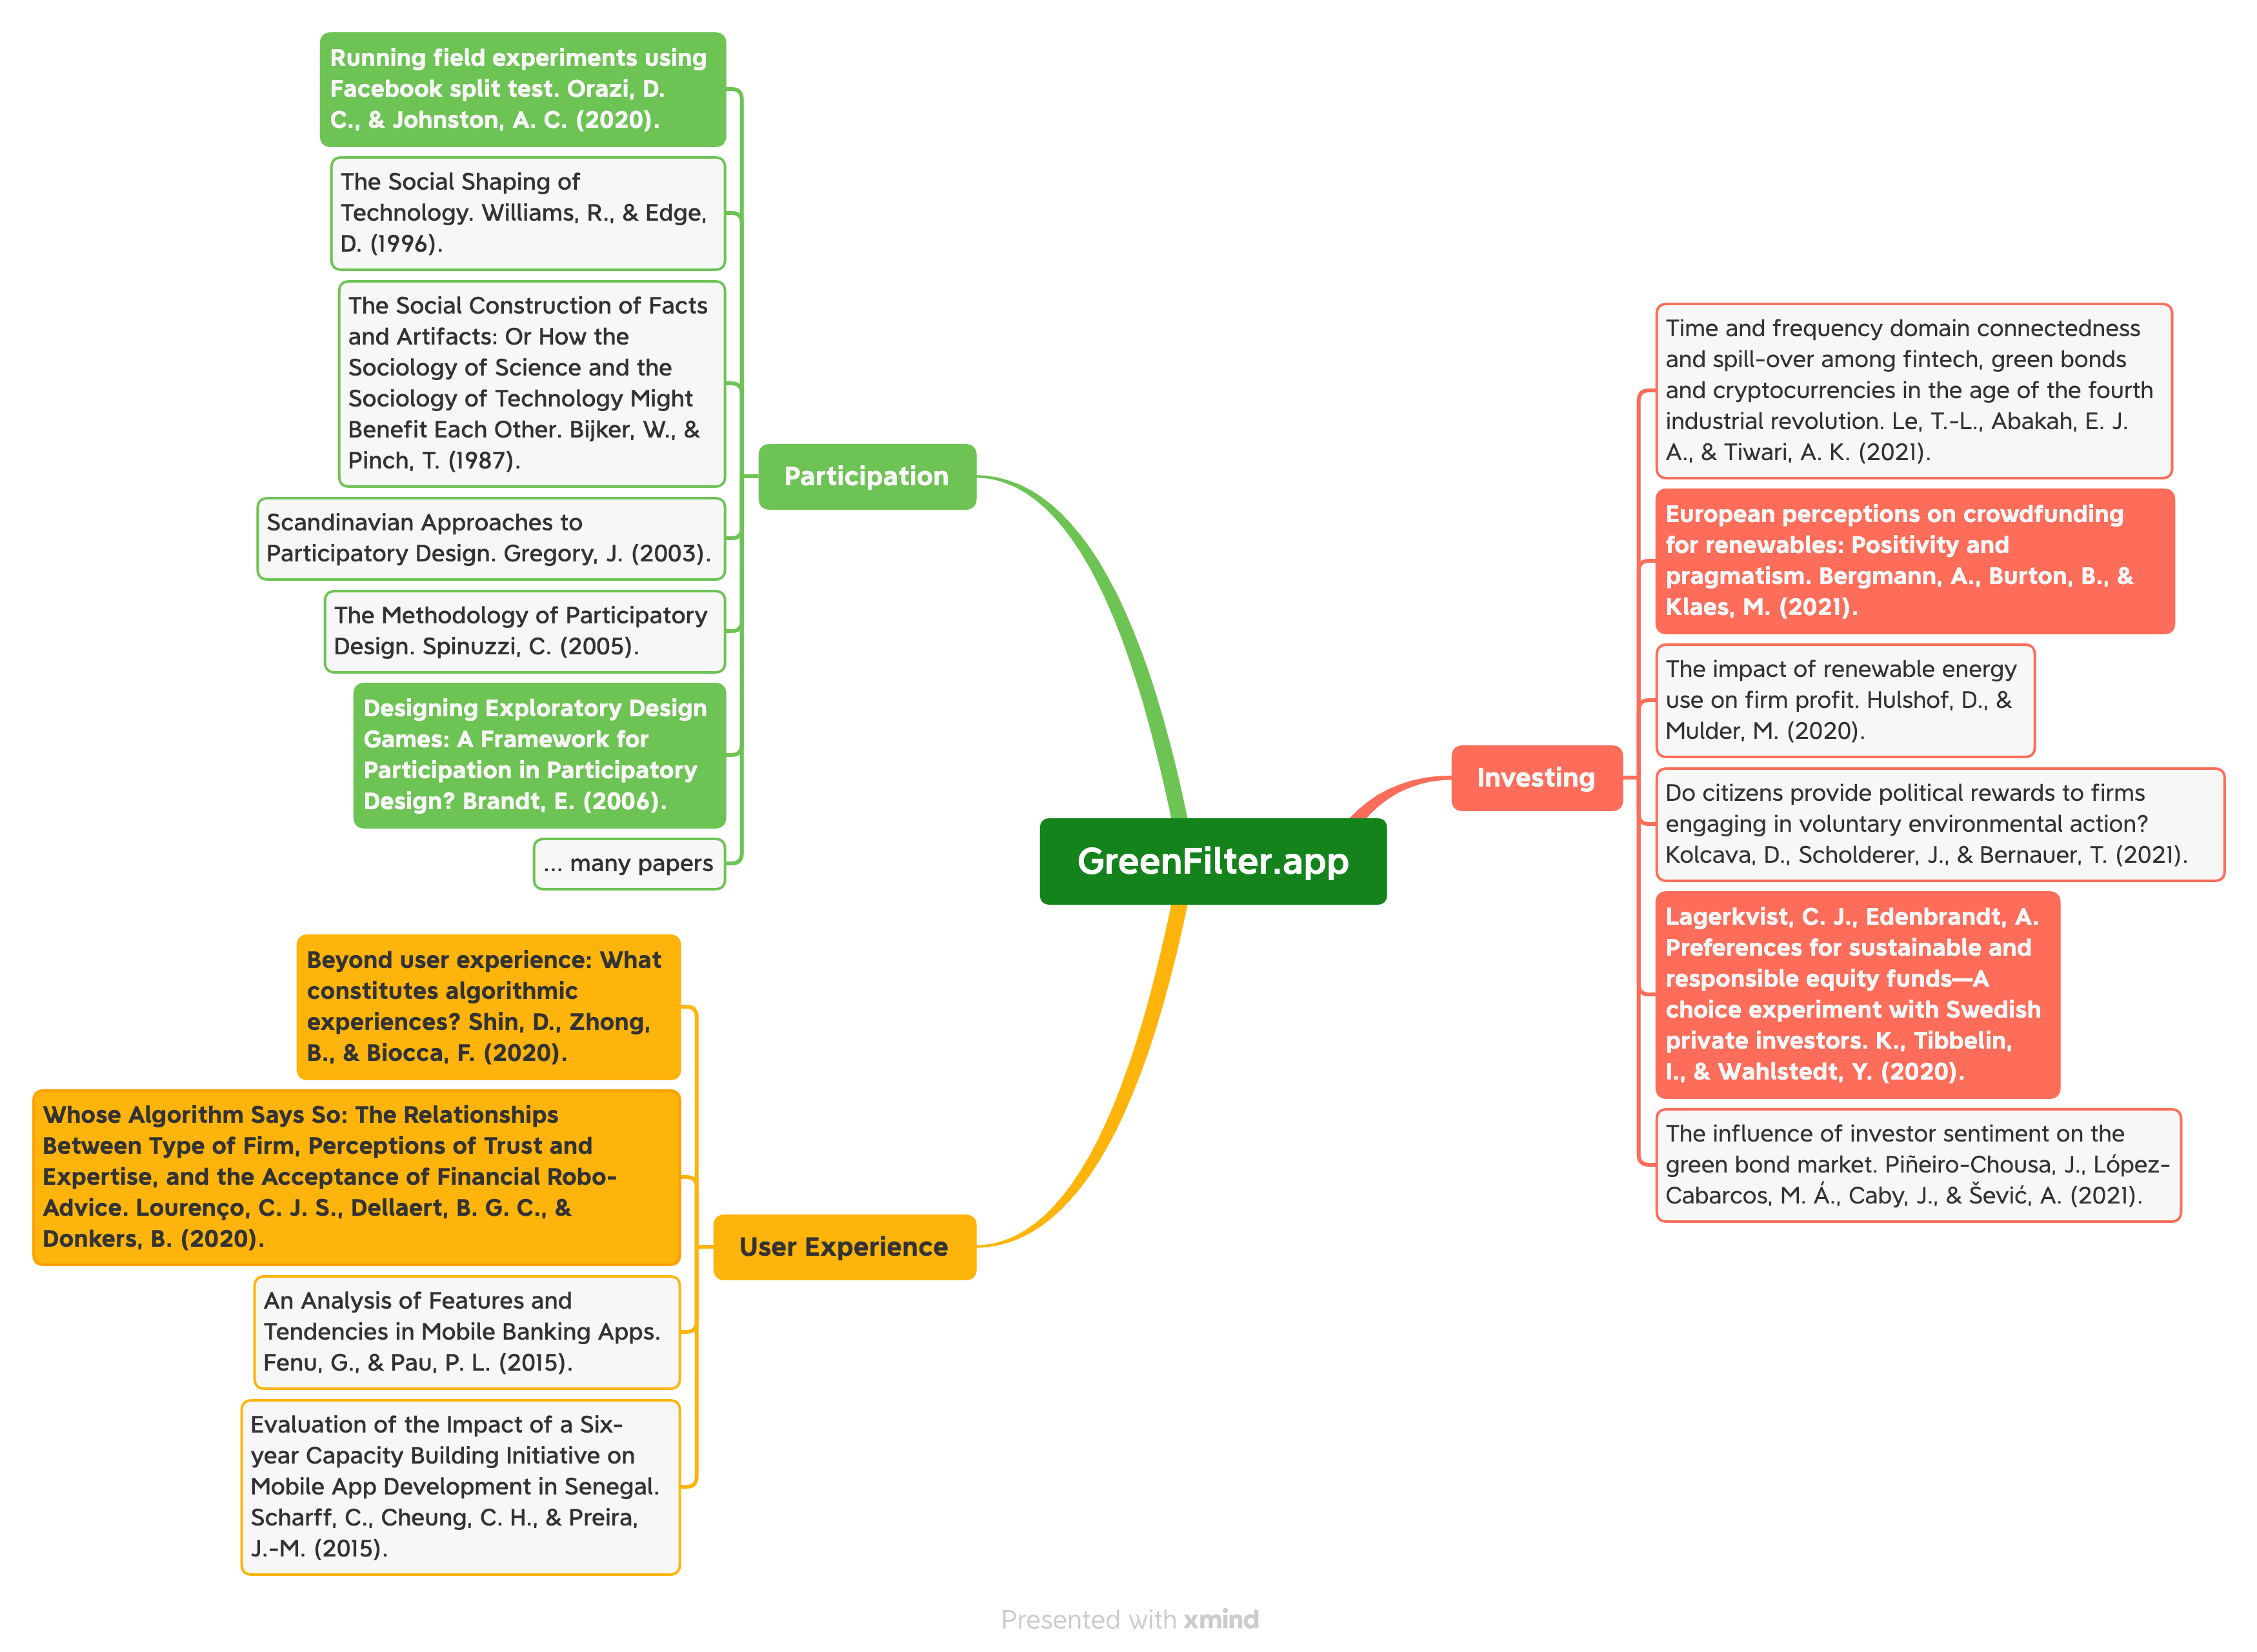
\includegraphics[width=1\linewidth,height=\textheight,keepaspectratio]{./images/literature/literature.png}

}

\caption{Example papers from the Literature Review}

\end{figure}%

This is a more complete concept map of the topics relevant to my
research.

\begin{figure}[H]

{\centering 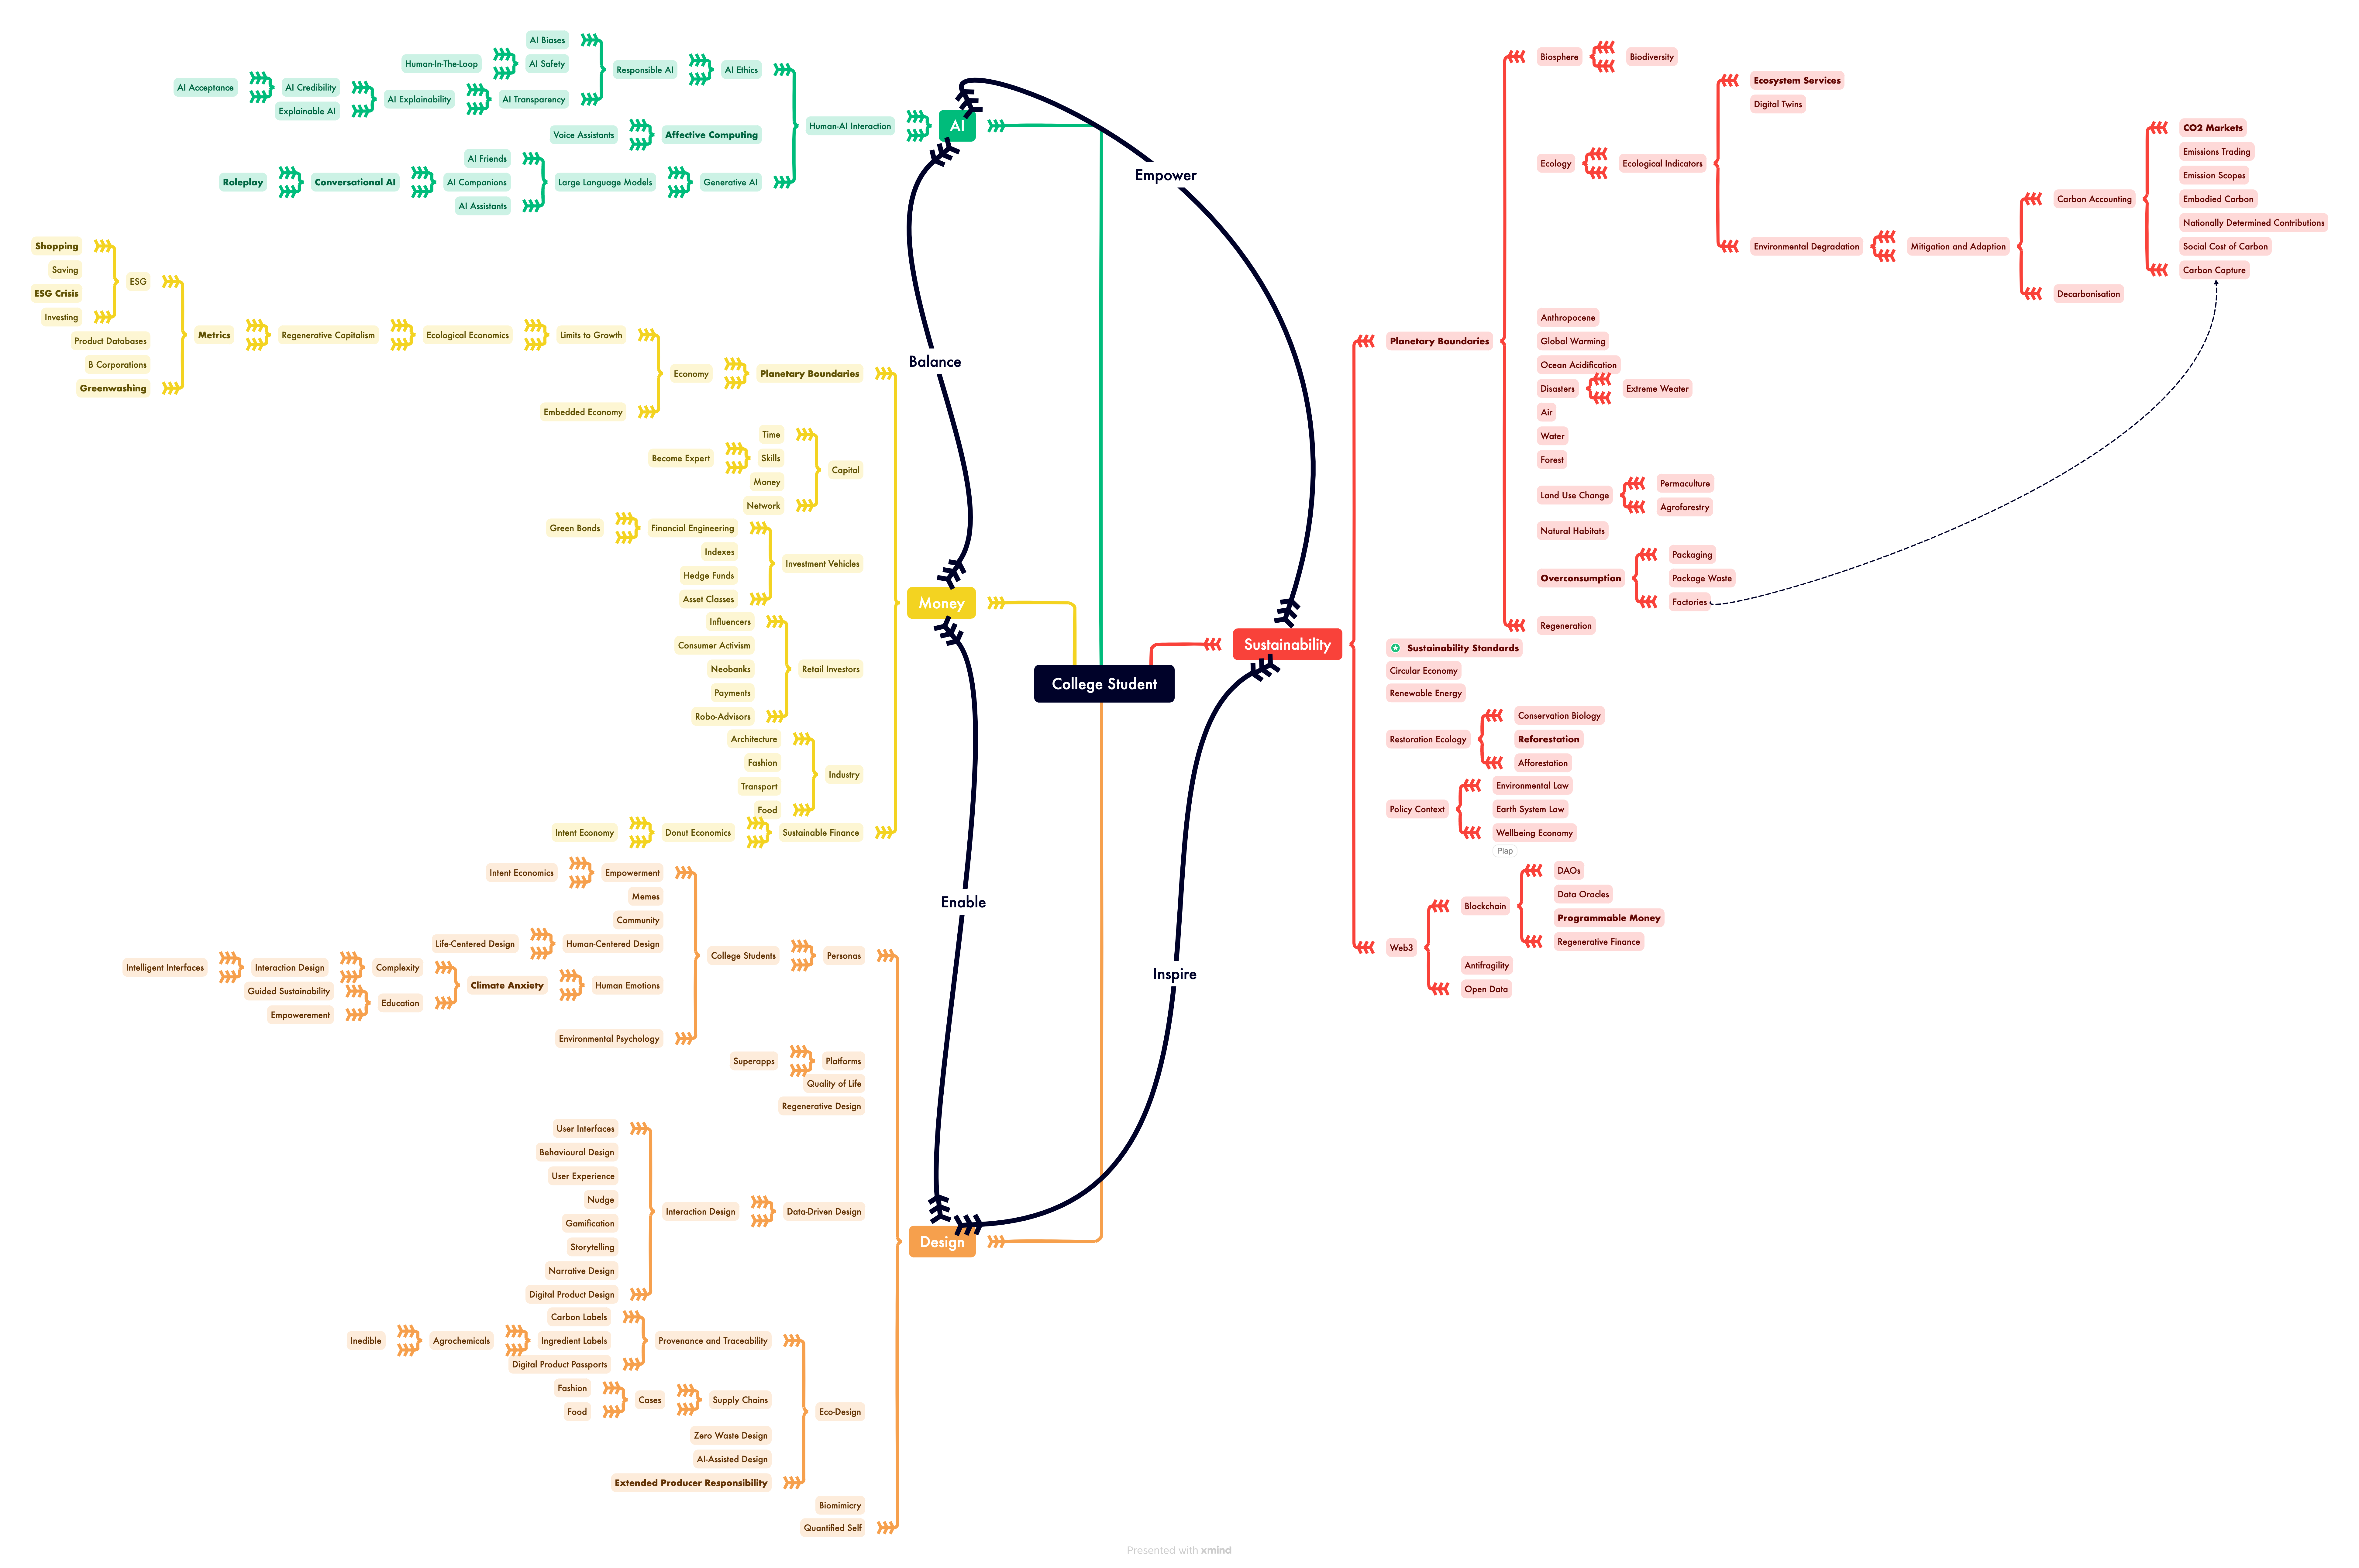
\includegraphics[width=1\linewidth,height=\textheight,keepaspectratio]{./images/literature/all.png}

}

\caption{Nearly Complete Concept Map}

\end{figure}%

\subsubsection{Goals}\label{goals}

Given the ambition of designing an app to integrate sustainable
shopping, saving, and investing, the goal of the literature review is to
find insights about the target audience (Taiwanese college students),
understand what kind of sustainable actions are effective, and translate
these into specific ideas for app features. In order to keep track more
easily, each literature review chapter provides \emph{design
implications} which are shown in the results section.

\subsubsection{Sources}\label{sources}

There is currently no single platform that hosts all scientific journals
leading me to source scientific papers from

\begin{enumerate}
\def\labelenumi{\arabic{enumi}.}
\tightlist
\item
  ScienceDirect
\item
  Nature
\item
  The Lancet
\item
  Oxford Academic
\item
  Semantic Scholar
\item
  JSTOR
\item
  Google search.
\end{enumerate}

\subsubsection{AI Use}\label{ai-use}

Statement of AI Usage in Research: I'm a long time AI-assistant user.

AI was used for:

\begin{enumerate}
\def\labelenumi{\arabic{enumi}.}
\tightlist
\item
  Search
\item
  Data comparison
\item
  Data science
\item
  Chart-building
\item
  Translation
\item
  Feedback
\item
  Editing
\item
  Spell-checking
\item
  Proofreading
\item
  Ranking citations' relevance to existing body of writing
\end{enumerate}

AI was \emph{NOT} used for writing.

A visualization of incremental changes (over a thousand Git commits) to
the thesis can be seen on the GitHub repository as well as in the
visualization below.

\newpage

\section{Young Adults and College
Students}\label{young-adults-and-college-students}

\subsection{Student Protests for Climate Justice: The World and
Taiwan}\label{student-protests-for-climate-justice-the-world-and-taiwan}

In August 2018, Swedish high-school student Greta Thunberg skipped class
to start a climate justice strike in front of the Swedish parliament
Riksdag. In 2019, Time magazine named Thunberg person of the year for
\emph{creating a global attitudinal shift} towards the environment
(Deutsche Welle, 2019). According to official statistics, 14 million
participants joined her \emph{Fridays for Future} strikes and the
movement expanded to over 7,500 cities around the world (Fridays For
Future, 2025). A survey 64 climate protesters from Norway, the UK, USA,
and Canada, found the climate-justice activists are non-homogeneous
group, displaying differing levels of factual knowledge about climate
change, a broad spectrum of emotions from anger to guilt and hope, with
diverse lifestyles, consumption habits, dietary shifts, and political
leanings (Martiskainen et al., 2020).

\begin{figure}[H]

{\centering 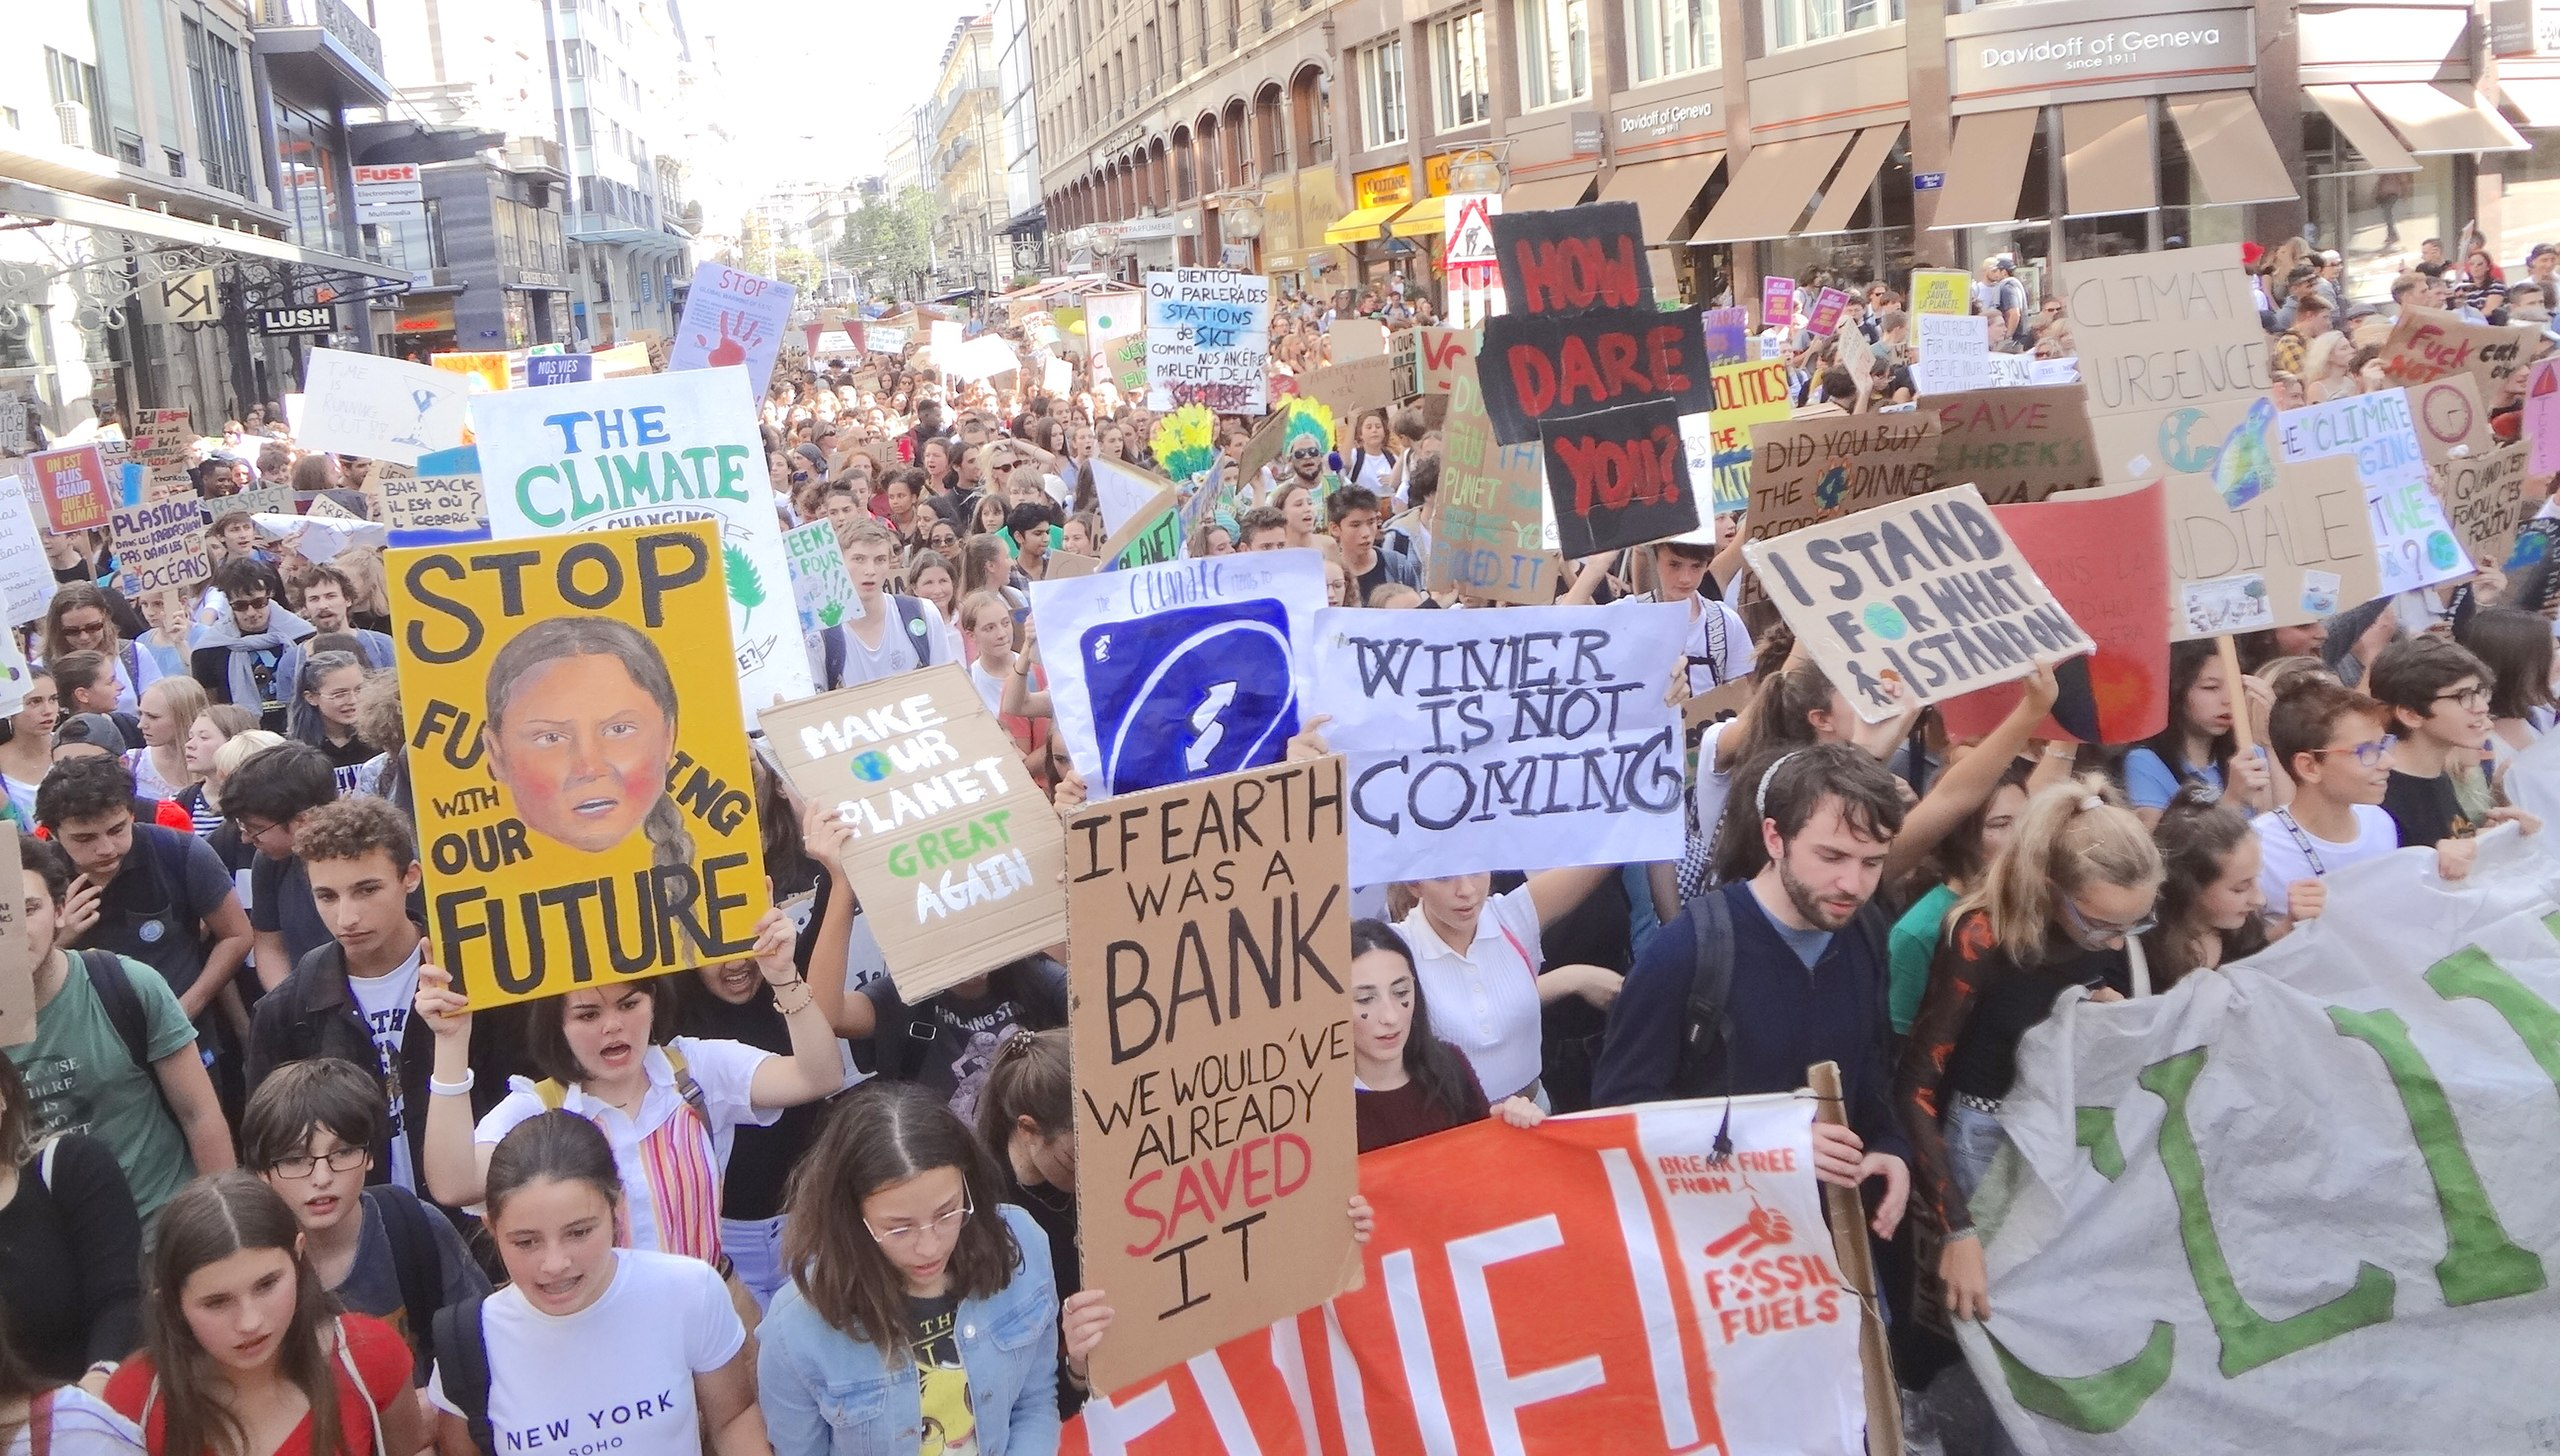
\includegraphics[width=1\linewidth,height=\textheight,keepaspectratio]{./images/college/geneve.jpg}

}

\caption{Climate protest in Geneva on September 27th, 2019 -- 1 year
after the start of Fridays for Future}

\end{figure}%

In Indonesia, which had large protests at the time, now 7 years later
activists are expressing disillusionment and frustration with the lack
of progress and upholding environmental promises. (Dwi Tamara, 2025)
reports on a survey of 382 Gen-Z respondents in 5 areas of Jakarta, with
99.5\% of the respondents having experienced extreme weather events
first-hand, highlighting how respondents were affected by
climate-related calamities, such as frequent flooding, which led to
students missing school days, - education which they are entitled to.
The Sharm El Sheikh climate policy implementation (UNFCCC, 2023b) text
refers to ``human right to a clean, healthy and sustainable
environment''. In Portugal, Estonia, and elsewhere young people have
moved on from strikes to actually taking legal action at the courts
suing companies for the environmental problems they have caused (Flor,
2024).

\begin{figure}[H]

{\centering 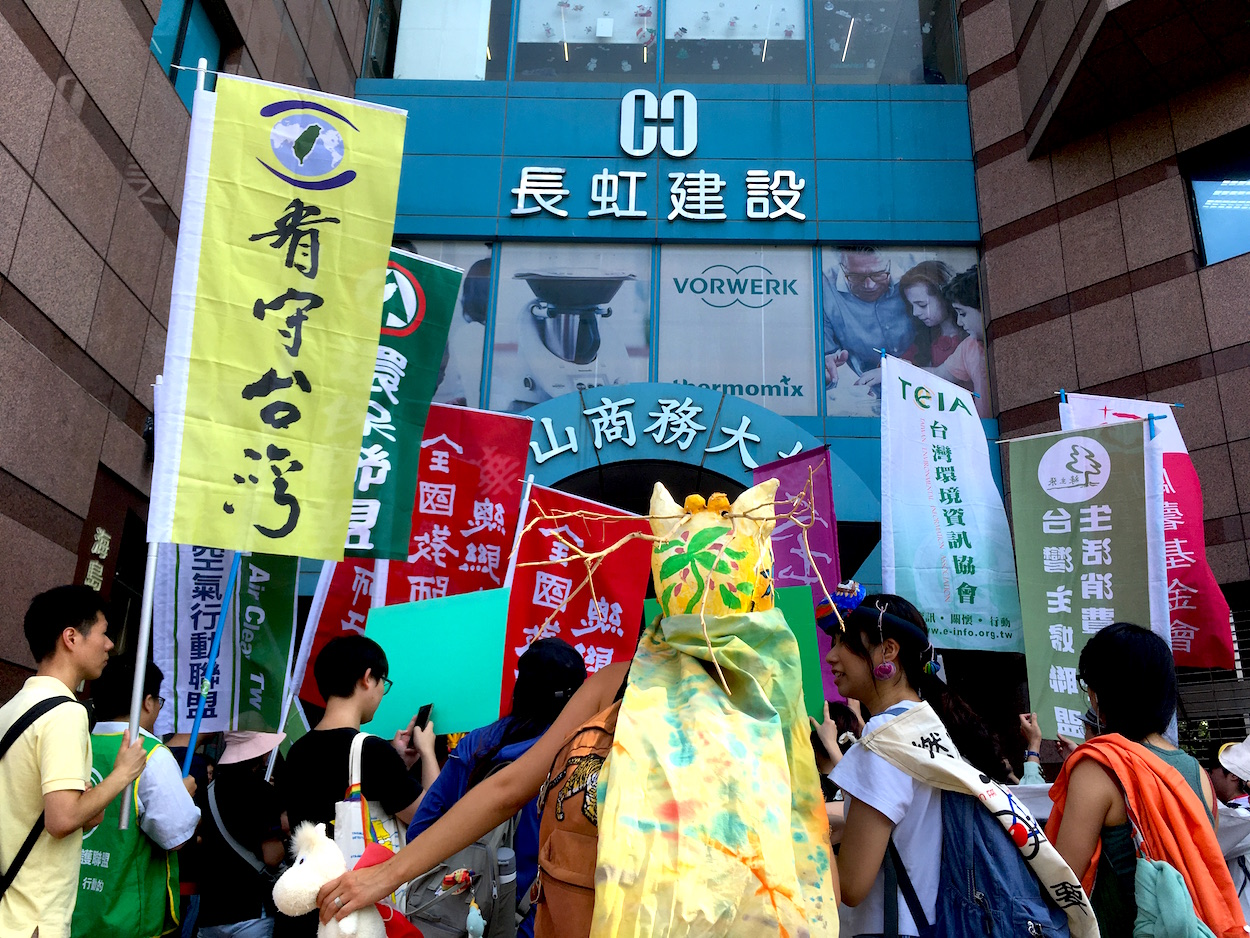
\includegraphics[width=1\linewidth,height=\textheight,keepaspectratio]{./images/college/taipei.jpg}

}

\caption{Climate protest in Taipei in May 2019 in front of the
Democratic Progressive Party (DPP) headquarters}

\end{figure}%

Meanwhile, as the climate-justice protests unfolded around the world, in
Taiwan, the Fridays for Future protests were very small in scale, with
no more than 100-200 people (Hioe, 2019). Meanwhile 2000 Taiwanese
students joined the initative by participating in environmental
activities without protesting (Dai, 2019). This could in part be
explained by Taiwanese culture being deeply influenced by Confucianism,
valuing stability, hierarchical relationships, academic excellence,
effort, and the role of education in achieving social status (R.-H. Xu,
2024). (H.-C. Chang, 2022) goes a step further to say that Taiwanese
youth are effectively unable to stage formal ``strikes'' due to
intersecting cultural constraints: obsession with academic performance,
low awareness of legal strike rights, and parental intervention --- so
they instead reframe actions as campus ``climate actions,'' exercising
agency within those limits. In addition, both Confucianism and Daoism,
the prevalent belief systems in Taiwan, affect education to be
\emph{teacher-centered}, where traditionally the role of students is to
listen and absorb knowledge; in today's society, there's space to open
opportunities for revisiting \emph{dialogue-based} education, where
students would be encouraged to take a more active role and gain
ownership of their education (C.-C. Chang et al., 2023).

\subsection{Taiwanese Educational System in
Numbers}\label{taiwanese-educational-system-in-numbers}

Taiwan has approximately 2 million young adults (Gen-Z, 18-26), and 73\%
percent of them are students attending tertiary education as of 2023,
with a slow increase of enrollment over the past decade (Ministry of
Education of Taiwan, 2024b).

\begin{figure}

\centering{

\pandocbounded{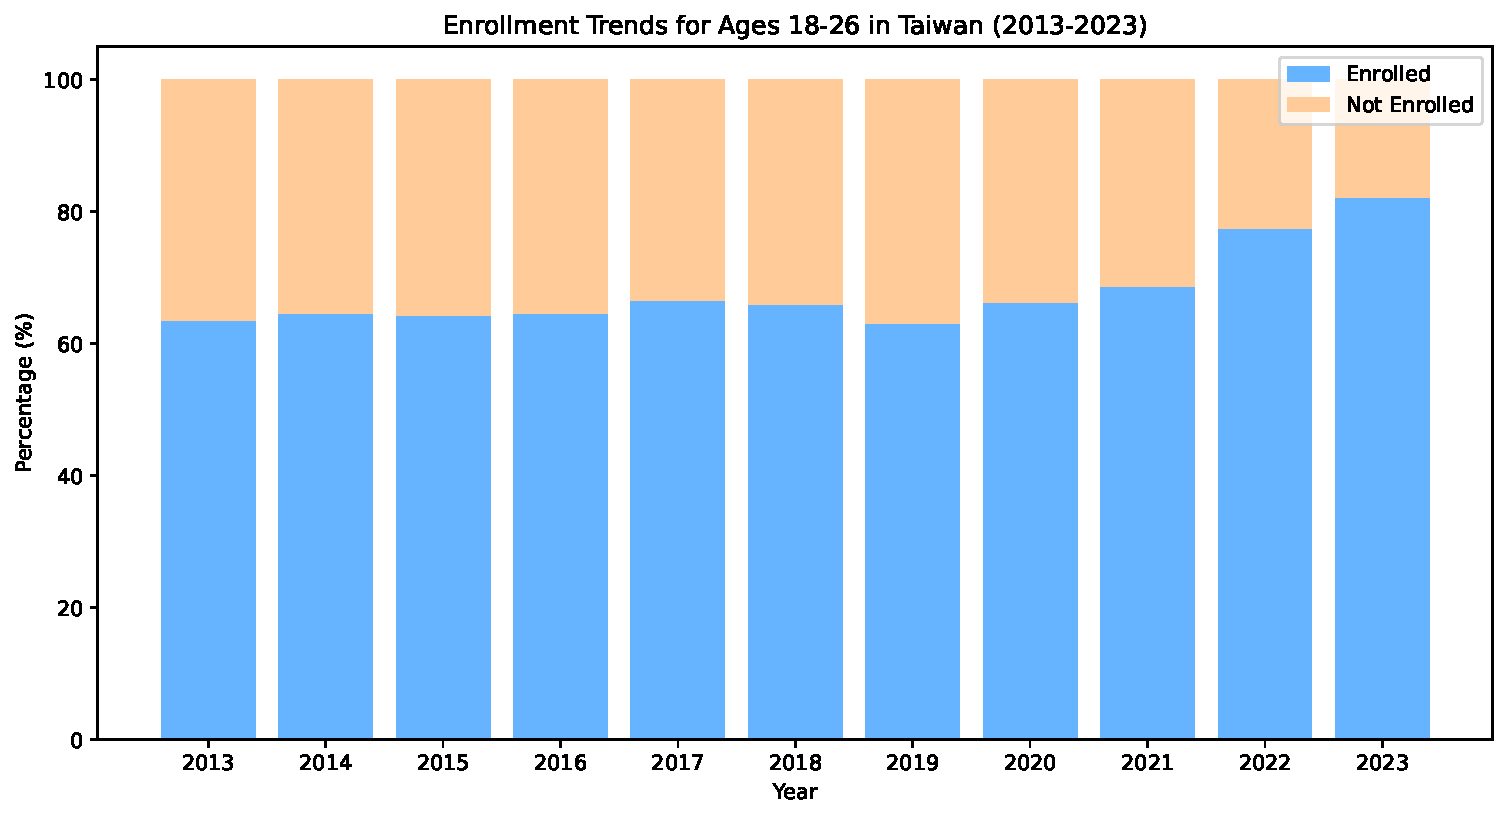
\includegraphics[keepaspectratio]{_thesis-nocite_files/figure-pdf/fig-tw-high-ed-enrollment-output-1.pdf}}

}

\caption[Enrollment in Taiwanese Higher
Education]{\label{fig-tw-high-ed-enrollment}Enrollment in Taiwanese
Higher Education}

\end{figure}%

As of 2024, Taiwan has a total of 148 universities, colleges, and junior
colleges (Ministry of Education of Taiwan, 2024c). Education funding is
4.26\% of Taiwan's GDP in 2023-24 and has been on a decline for a decade
(Ministry of Education of Taiwan, 2024a). Taiwan has an aging population
and declining birth rates have forced several schools to close down
(Davidson \& Chi-hui, 2024; Goh et al., 2023).

\begin{figure}

\centering{

\pandocbounded{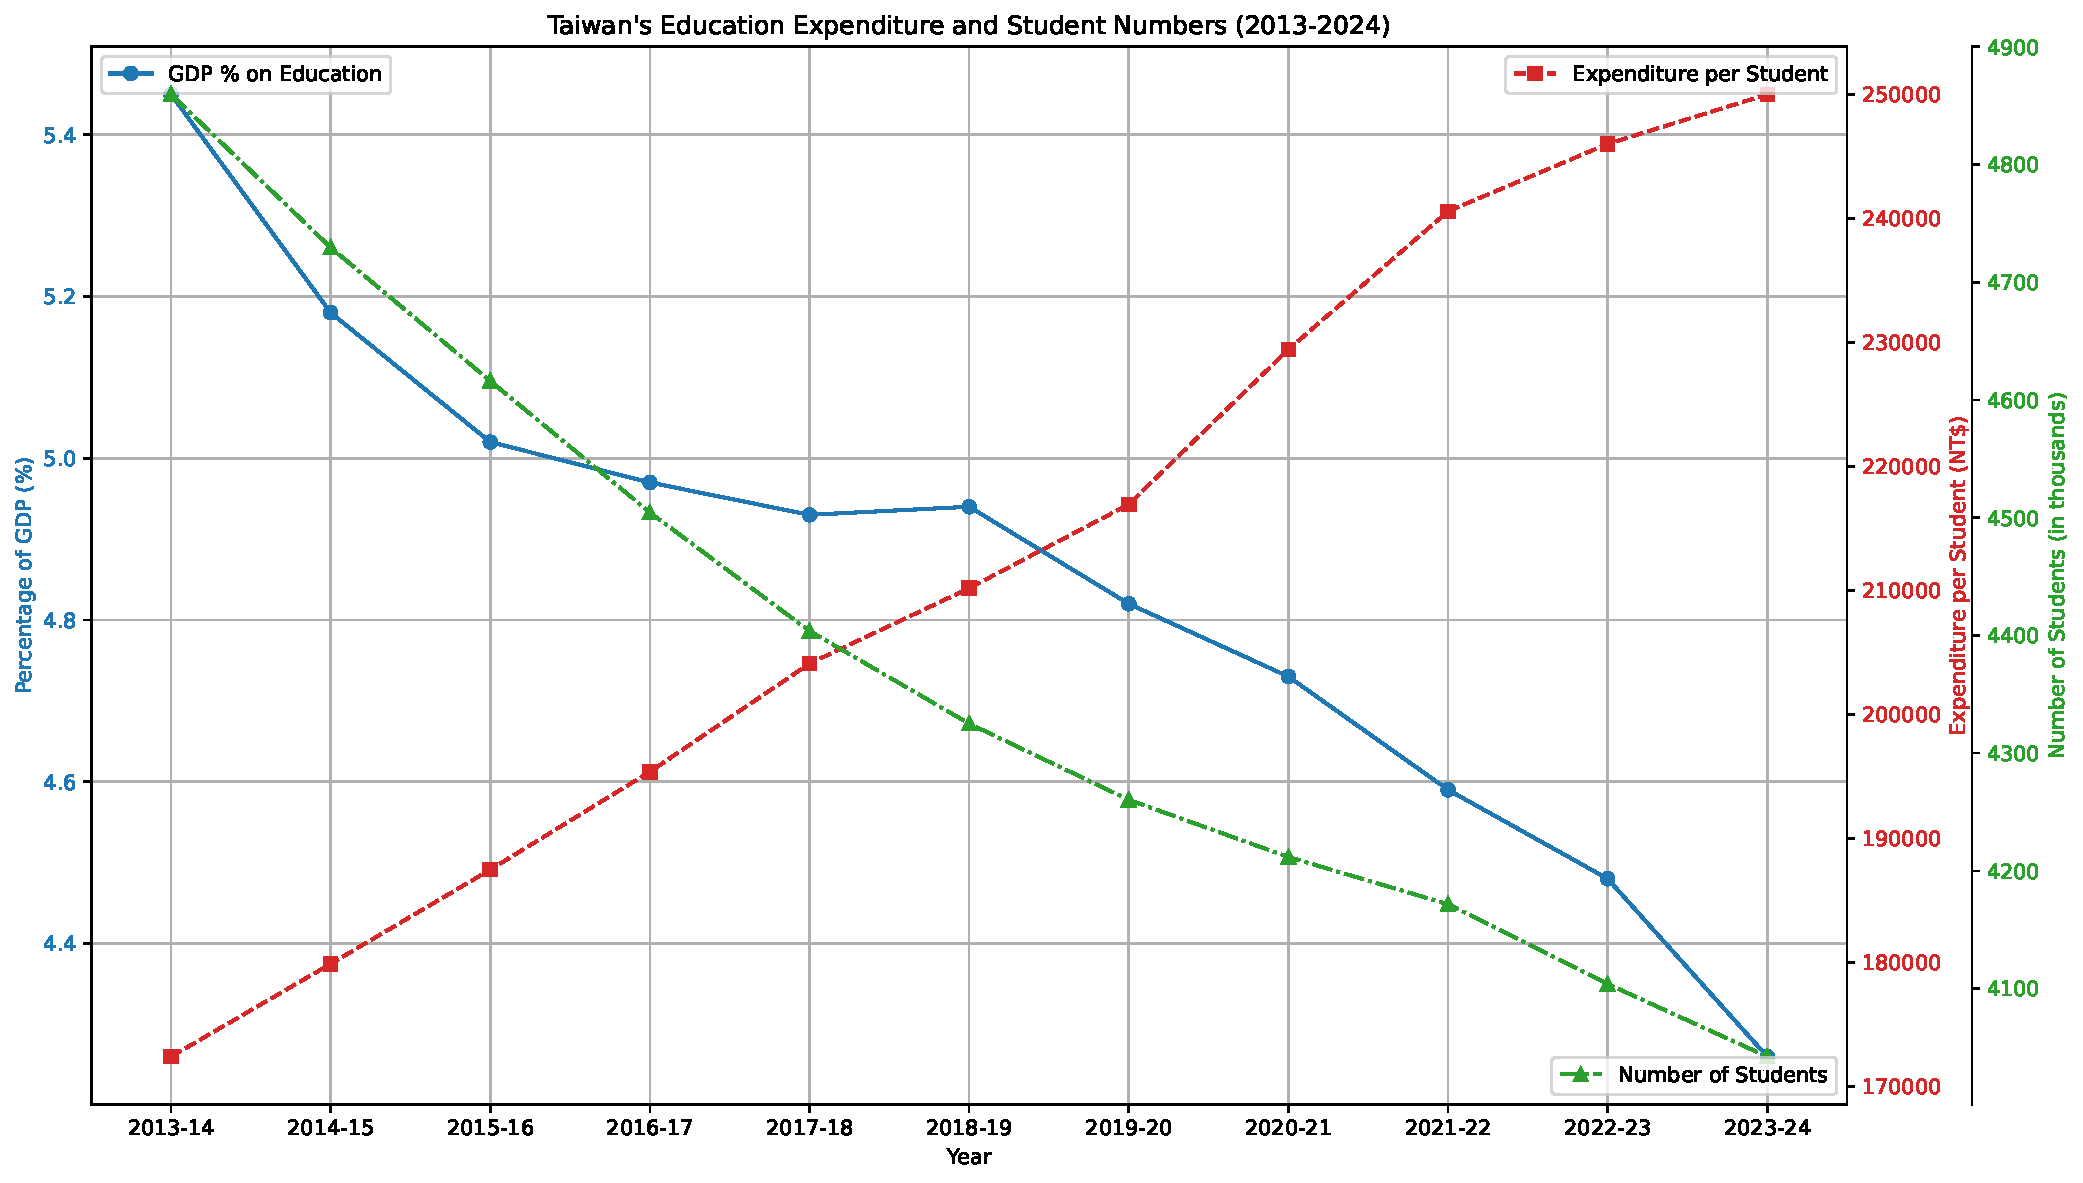
\includegraphics[keepaspectratio]{_thesis-nocite_files/figure-pdf/fig-tw-high-ed-funding-output-1.pdf}}

}

\caption[Funding for Taiwanese Higher
Education]{\label{fig-tw-high-ed-funding}Funding for Taiwanese Higher
Education}

\end{figure}%

While the overall number of students is declining, the share of
international students is increasing.

\begin{figure}

\centering{

\pandocbounded{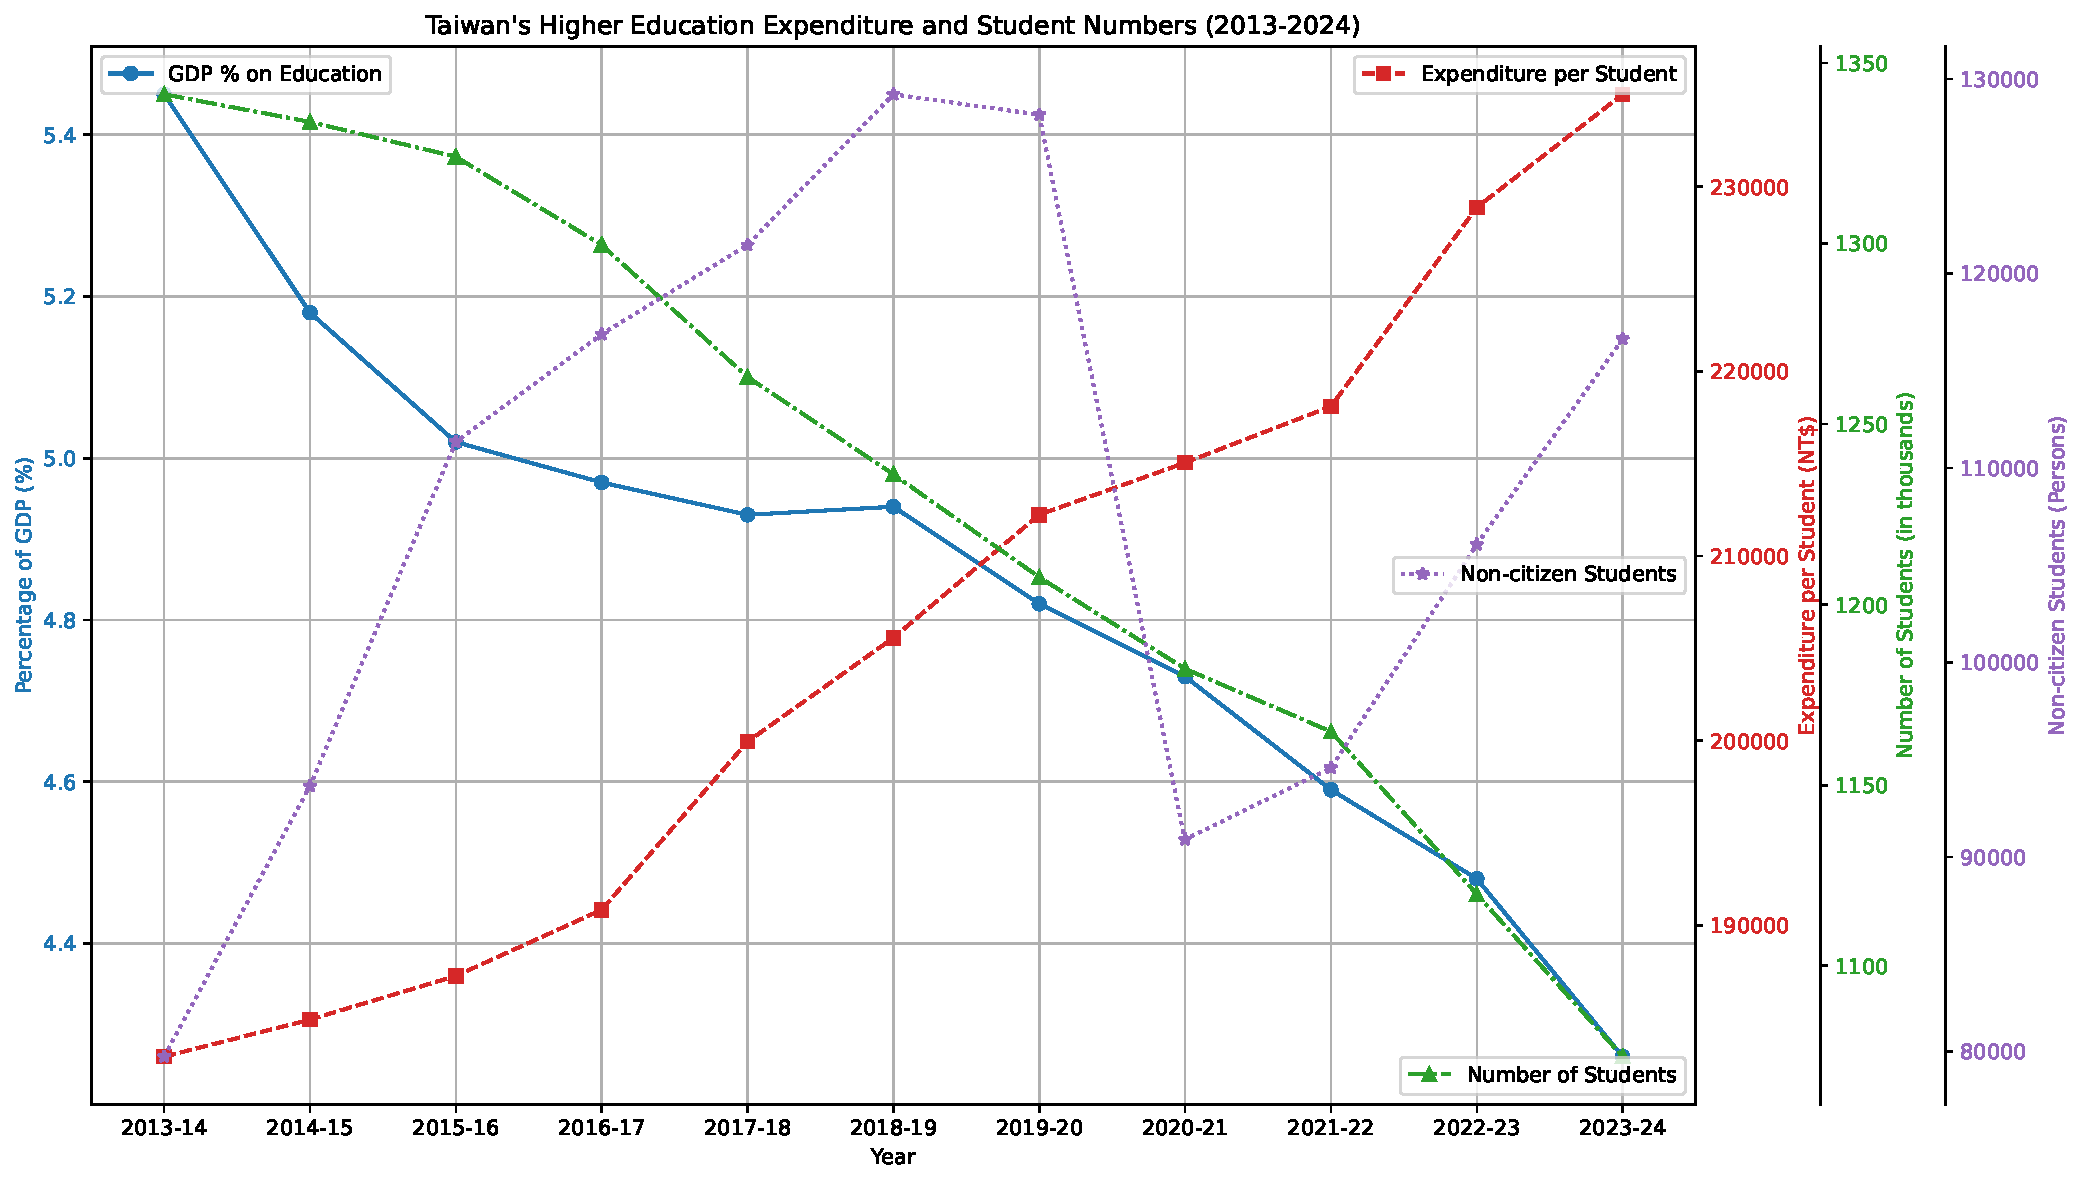
\includegraphics[keepaspectratio]{_thesis-nocite_files/figure-pdf/fig-tw-high-ed-output-1.pdf}}

}

\caption[Demographics of Taiwanese Higher
Education]{\label{fig-tw-high-ed}Demographics of Taiwanese Higher
Education}

\end{figure}%

\subsection{Designing for College Students: Developing
Personas}\label{designing-for-college-students-developing-personas}

Students in the Generation-Z age bracket (abbreviated as Gen-Z or
Zoomers) are born between 1997 and 2012 (Branka Vuleta, 2023). High
levels of technology adoption worldwide (Deyan Georgiev, 2023a). Over
98\% of Gen-Z owns a smartphone while only 80\% of the general world
population does (BankMyCell, 2022; Global Web Index, 2017).

Designing for College Students: Developing Personas. User research makes
extensive use of user \emph{personas} to represent a group of people
with similar attributes. Designers use personas to \emph{articulate
assumptions,} which, if used well, is useful for \emph{user-centered
design}, to create better products. Personas help to reflect on what
kind of \emph{biases} might exist in the design. Within the larger
cohort of college students several different personas could be defined,
for example grouping people by interests, knowledge, habits, levels of
anxiety, and other attributes. Humans have a long list of cognitive
biases, which a good design should take into account.

Many general observations can be made, however to create meaningful
personas, these should be backed up with data. Students ride bicycles
and scooters. Many circular economy service such as YouBike and
transport sharing platforms like Uber are available in Taiwan. Many
students live in dorms and shared housing, meaning their impact per
square meter is low.

\subsection{Taiwanese Youth in Global Context: Sustainability Attitudes
From Eco-Friendly Diet to Climate
Action}\label{taiwanese-youth-in-global-context-sustainability-attitudes-from-eco-friendly-diet-to-climate-action}

Addressing the Research Gap When it Comes to Taiwanese College Students.
There's lack of scientific research when it comes to Taiwanese college
students, not only in English or other foreign languages, but also in
Chinese. Much of the research in Taiwan focuses on younger students,
particularly those in primary and secondary schools. With regard to
issues related to college students and sustainability, even less
research is available. My project hopes to shed some light to how
Taiwanese college students relate to sustainability.

(Kuo-Hua Chen, 2019) compares Taiwan to other countries in terms of
\emph{Postmaterialist Index Comparison}, noting Taiwanese society is
materialistic.

\begin{figure}

\centering{

\pandocbounded{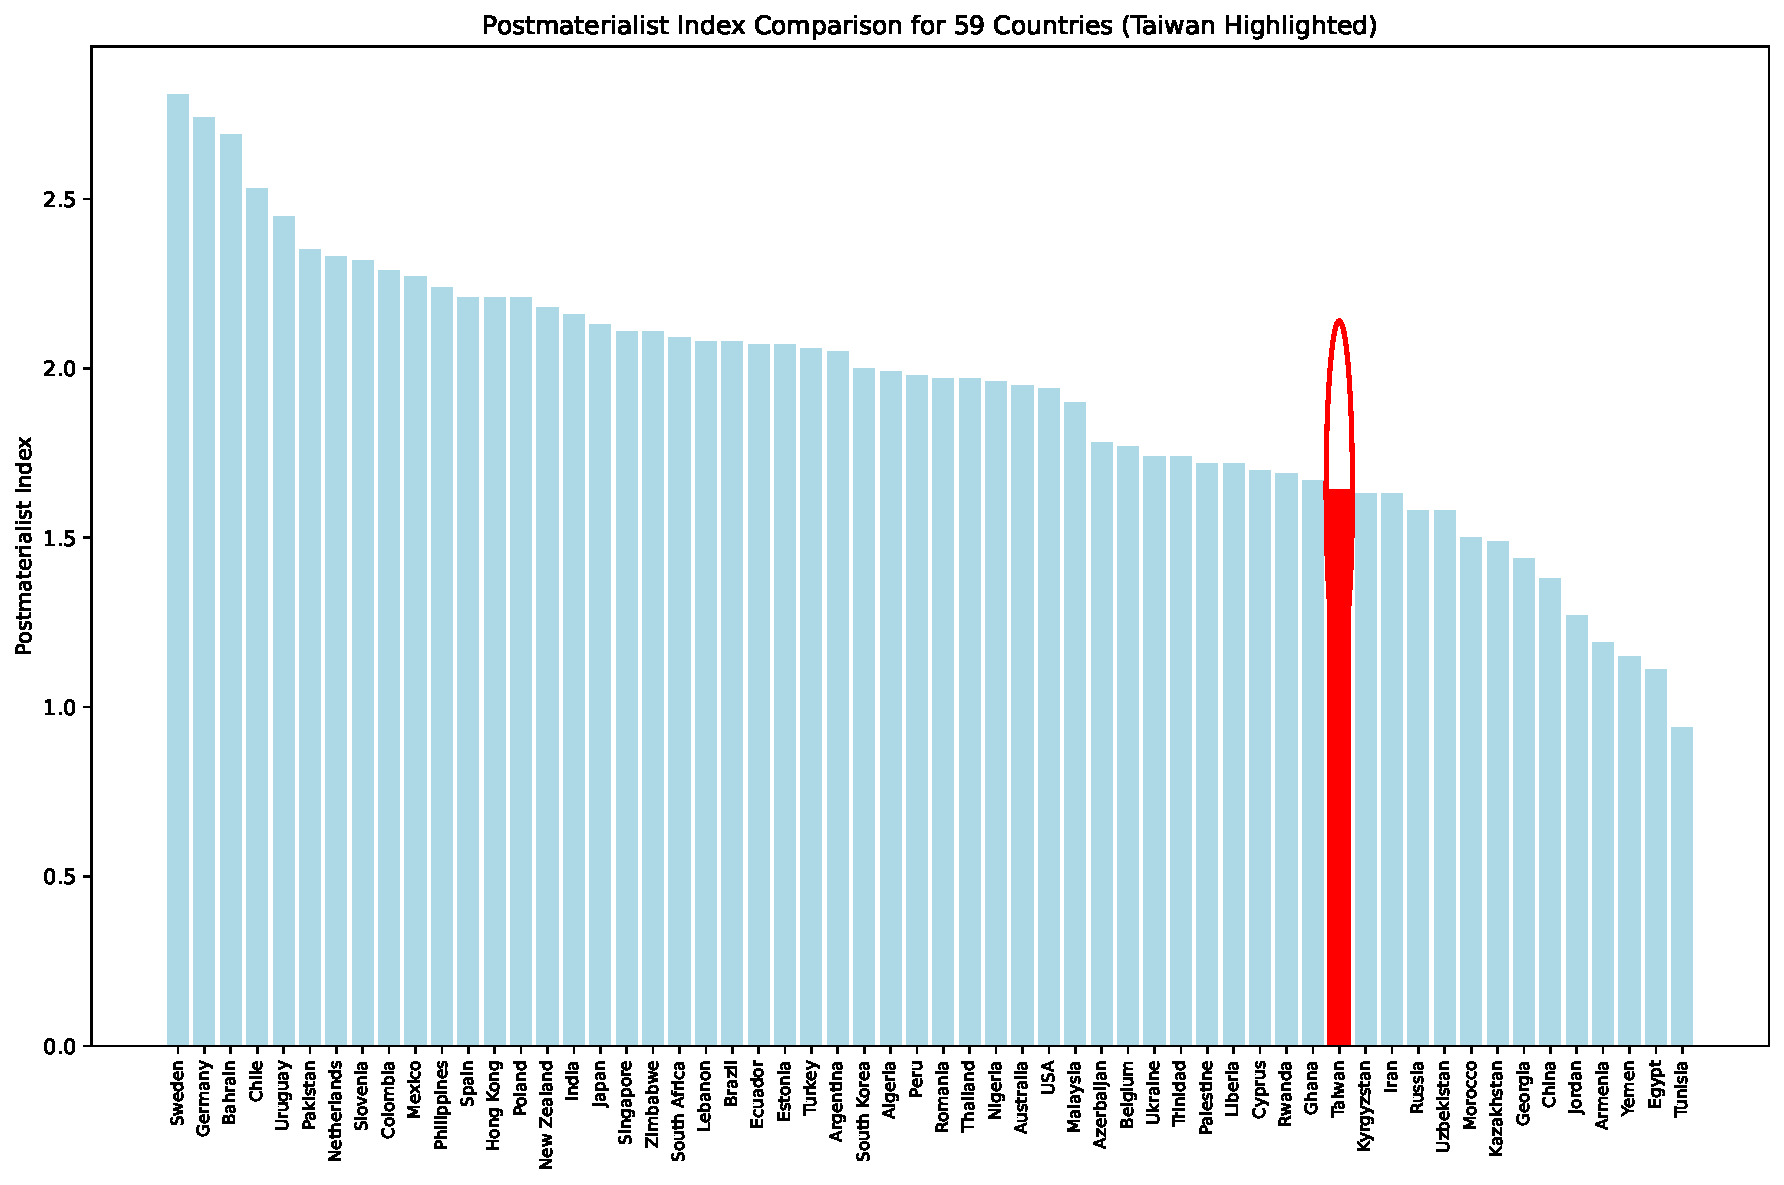
\includegraphics[keepaspectratio]{_thesis-nocite_files/figure-pdf/fig-postmat-index-output-1.pdf}}

}

\caption[Postmaterialist Index (Taiwan
Highlighted)]{\label{fig-postmat-index}Postmaterialist Index across 59
countries (Taiwan highlighted)}

\end{figure}%

World Values Survey

\begin{figure}

\centering{

\pandocbounded{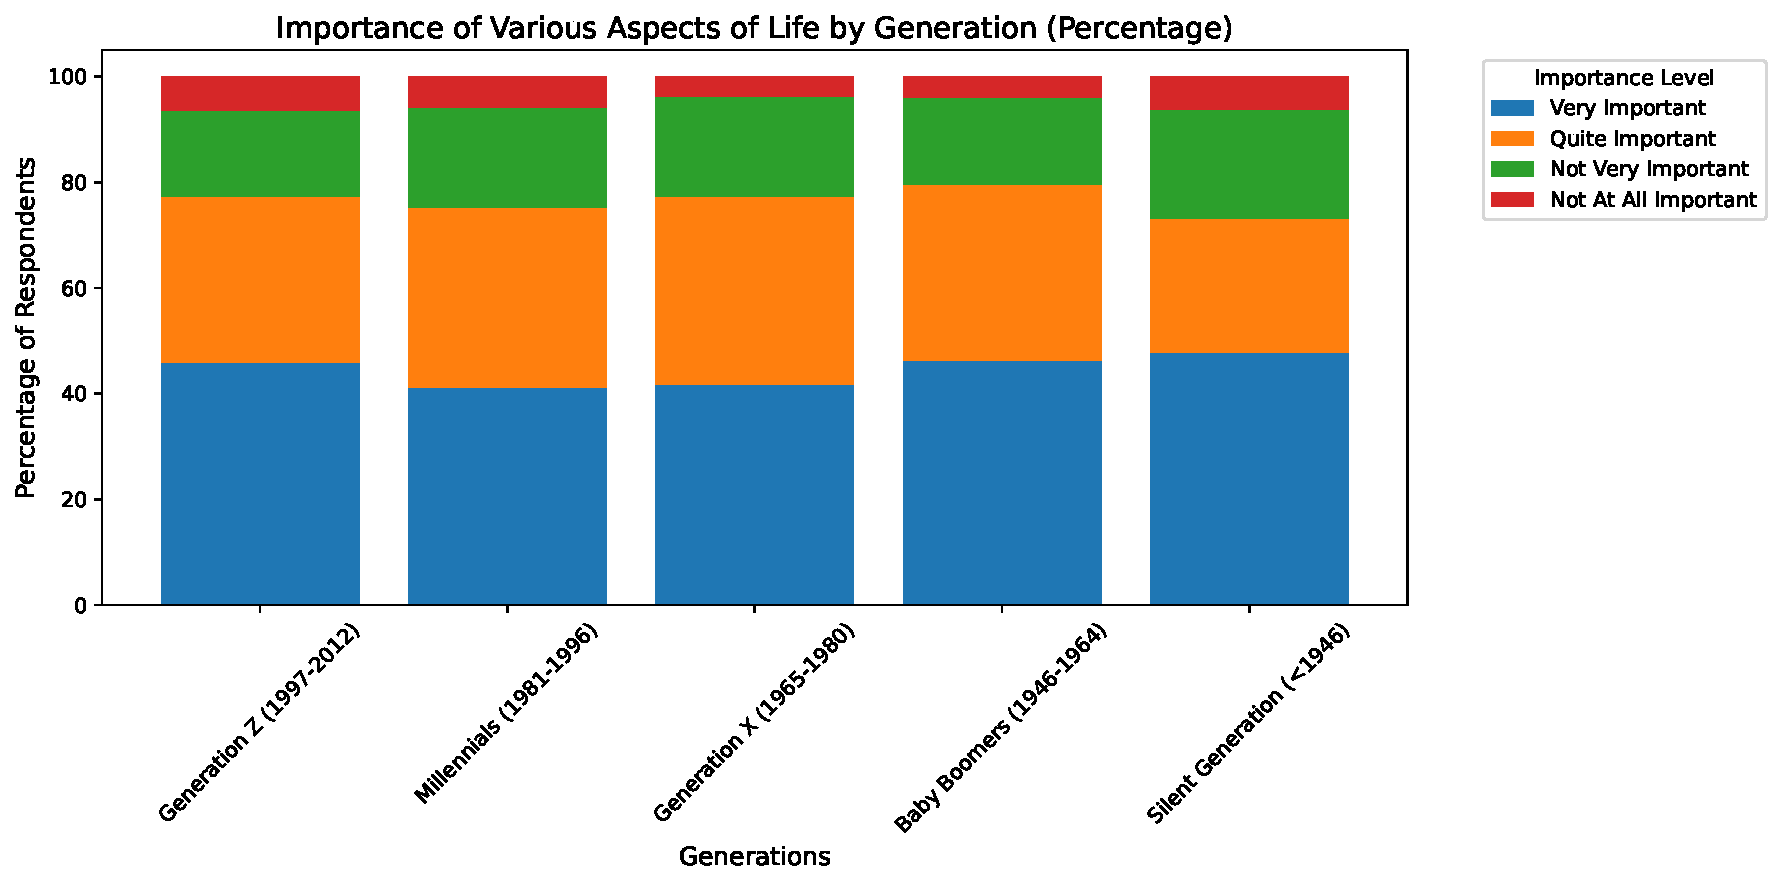
\includegraphics[keepaspectratio]{_thesis-nocite_files/figure-pdf/fig-world-values-output-1.pdf}}

}

\caption[World Values Survey]{\label{fig-world-values}World Values
Survey}

\end{figure}%

(Franzen \& Bahr, 2024) measures \emph{``mean environmental concern''}
to look at decade-level changes in societal environmental attitudes
across countries. Taiwan's general attitudes have stayed almost the same
(slight increase). The UK has had the largest jump in concern.
Curiously, South Korea has had a slight decrease in concern. Slovakia
and Russia were not very concerned with the environment a decade ago and
are even less concerned now.

A large, global-scale study by (Anthony Leiserowitz et al., 2022)
administered on Meta's Facebook (n = 108946) reported people in Spain
(65\%), Sweden (61\%), and Taiwan (60\%) believe \emph{``climate change
is mostly caused by human activities''}.

\begin{figure}

\centering{

\pandocbounded{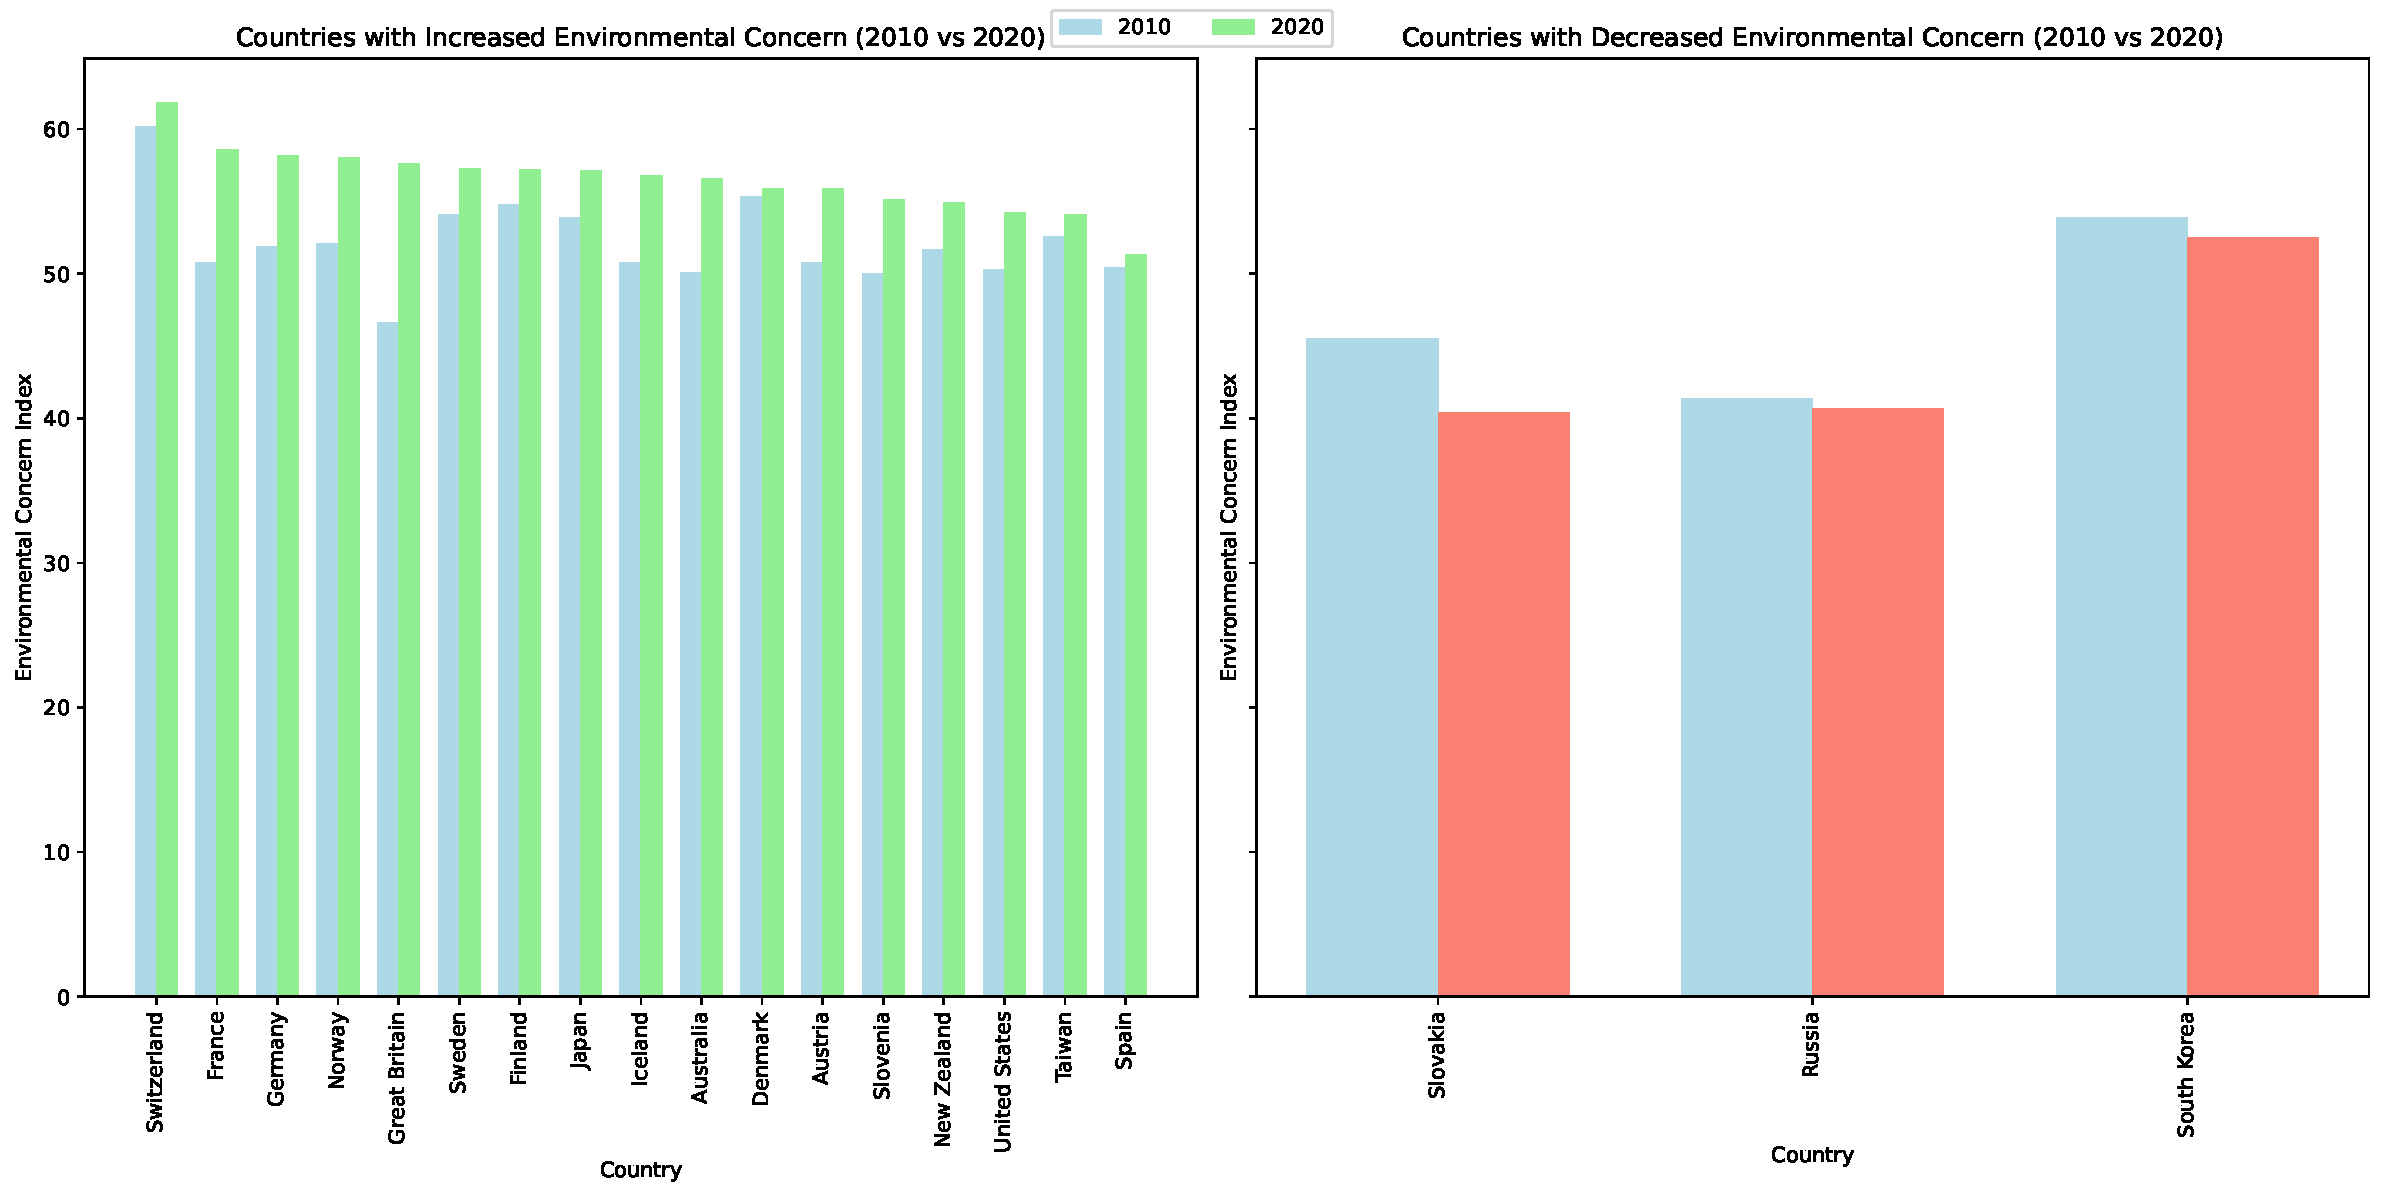
\includegraphics[keepaspectratio]{_thesis-nocite_files/figure-pdf/fig-global-climate-attitudes-output-1.pdf}}

}

\caption[Global Attitudes Towards Climate
Change]{\label{fig-global-climate-attitudes}Global Attitudes Towards
Climate Change}

\end{figure}%

The largest study to date, conducted by the United Nations across 50
countries, surveying 1.2 million people, distributed through mobile game
ads, showed the majority of people agreeing climate change is an
``emergency'' (UNDP, 2021).

\def\pandoctableshortcapt{UN Survey: 1.2 Million Responses to
\emph{Climate Change Is An Emergency}}

\begin{longtable}[]{@{}lll@{}}
\caption[UN Survey: 1.2 Million Responses to *Climate Change Is An
Emergency*]{1.2 million UN survey responses to the statement ``Climate
change is an emergency''.}\tabularnewline
\toprule\noalign{}
\endfirsthead
\endhead
\bottomrule\noalign{}
\endlastfoot
Age Group & Agree & Neutral or Disagree \\
18-35 & 65\% & 35\% \\
36-59 & 66\% & 34\% \\
Over 69 & 58\% & 42\% \\
\end{longtable}

\let\pandoctableshortcapt\relax

At the pre-university level, Taiwanese government has been promoting
environmental education through a green school network; however surveys
at middle school and high school level suggest there is no impact on
\emph{sustainability consciousness} among students in comparison with
regular schools (Olsson et al., 2019). Rather, Taiwanese students are
influenced towards environmental action by \emph{group consciousness}
(T.-Y. Yu et al., 2017). In contrast,(陳珮英, 2003) reports \emph{good
knowledge of sustainable development} topics among \emph{junior high
school students} in Da-an District, Taipei City (n =596). (林建輝.,
2009) similarly reports a positive attitude and good knowledge of
environmental sustainable development among senior \emph{high school
students} towards in Taipei City (n = 328). Several Taiwanese studies
also focus on the physical environment of school campuses, for example
the sustainability of elementary school campuses (潘智謙 \& Pan, 2006).
Elementary-school teachers in Taichung (n = 536), have positive
attitudes towards environmental education are positive, proactive and
demonstrate high awareness; they have participated in many
sustainability-related workshops (Liao et al., 2022).

At the university level, (C.-L. Chen \& Tsai, 2016) reports a
\emph{positive attitude yet moderate knowledge} about \emph{ocean
sustainability} among Taiwanese college students (n = 825). (C.-H. Liu
et al., 2023) studied sustainability behavior of Taiwanese University
students, reporting the COVID-19 pandemic, in addition to prevalence of
health issues, also spurred more attention on environmental topics. In a
similar vein, the devastating nuclear disaster in Fukushima, Japan,
after 2011 earthquake, had an effect on Taiwanese energy and
sustainability education (姚 \& 侯, 2011). Taiwanese government launched
the Sustainable Council in 1997 to promote of environmental and
sustainable development; a survey of university-level teachers (n = 100)
in central Taiwan (Taichung, Changhua, and Yunlin) shows a positive
attitude toward environmental sustainability among teachers however
implementation of environmental sustainability practices is from low to
medium range (林美惠. \& 莊, 2015). Taiwanese government has also
launched funding for University Social Responsibility (USR) programs to
train college students in social innovation and local revitalization (D.
Chen \& Chou, 2023; W.-H. Liu et al., 2022). In general, it could be
concluded, Taiwanese students and teachers at all levels of education
have a positive attitude towards sustainability (Note: which is not a
very actionable finding).

Comparing college students' education for sustainable development (ESD)
in Taiwan (n = 617) and Sweden (n = 583) found Sweden has a long history
in environmental education while in Taiwan environment became a focus
area with the 1998 educational reform (Berglund et al., 2020).

\begin{figure}

\centering{

\pandocbounded{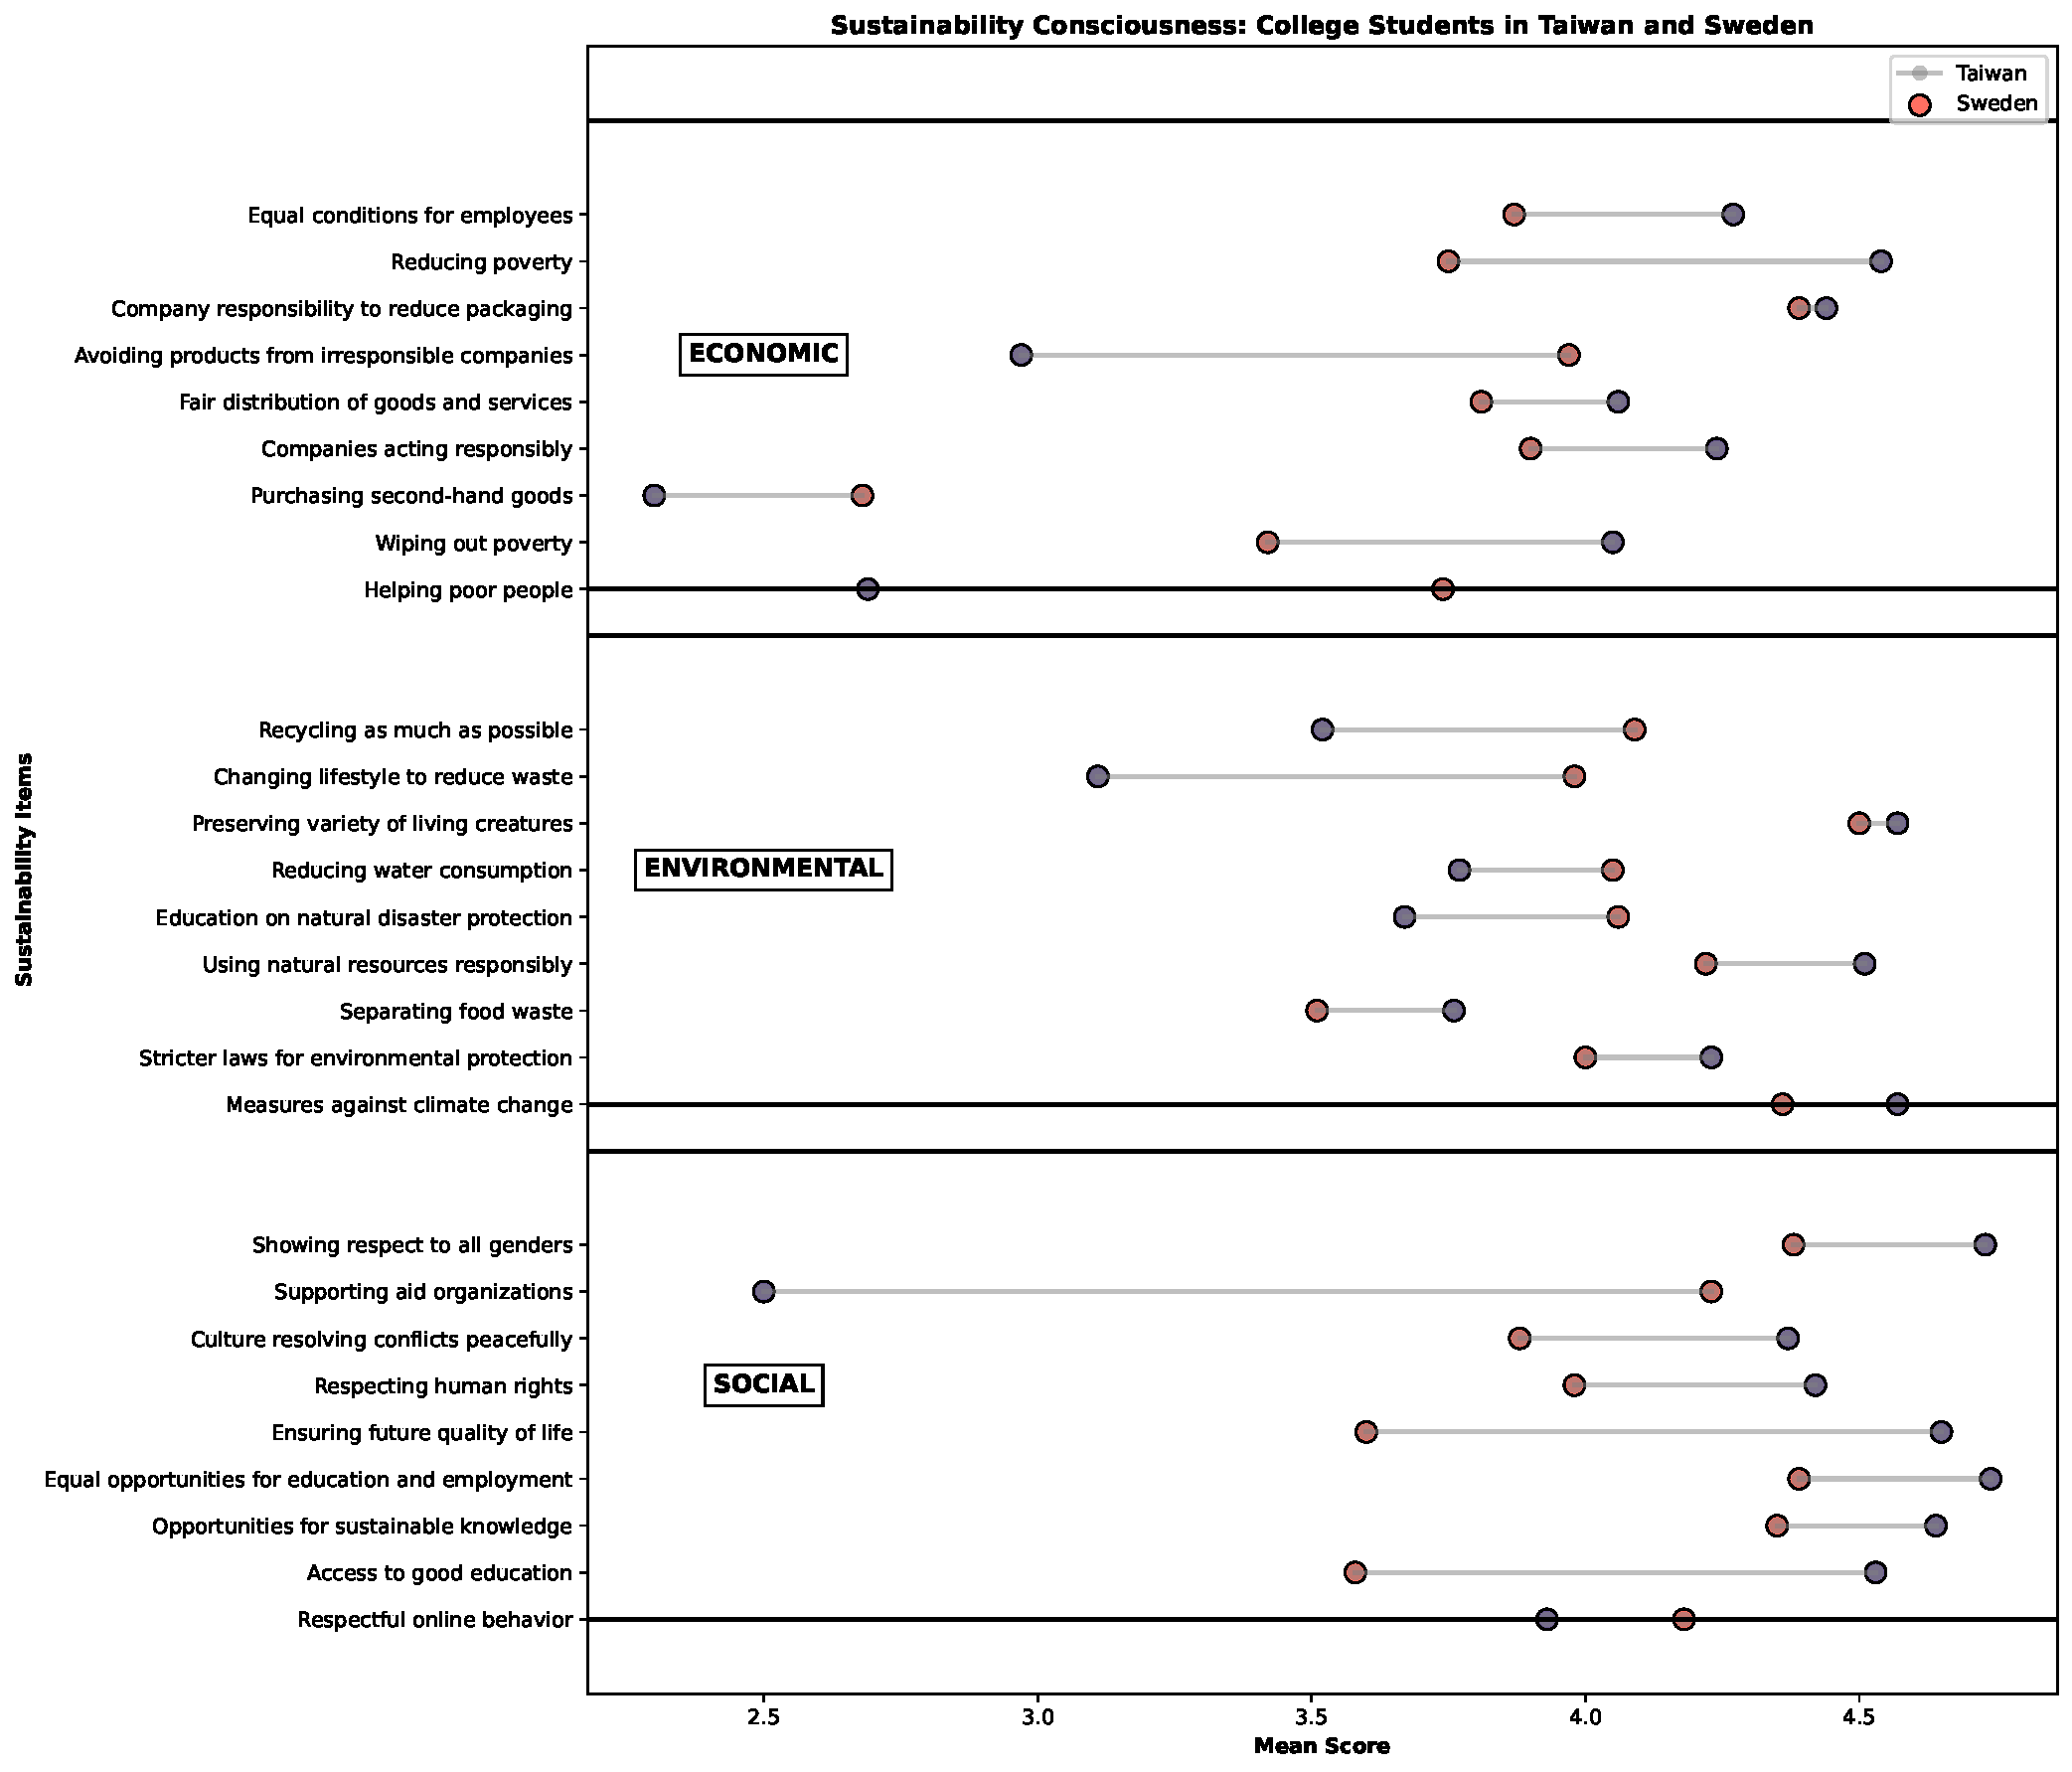
\includegraphics[keepaspectratio]{_thesis-nocite_files/figure-pdf/fig-tw-swe-output-1.pdf}}

}

\caption[College Students' Sustainability Education: Taiwan vs
Sweden]{\label{fig-tw-swe}Comparing college students' education for
sustainable development in Taiwan and Sweden}

\end{figure}%

An older study in 5 university in Taipei and Taichung (n = 255) found
78.04\% of respondents consumed beef in the month prior and were
concerned with food safety, freshness, and quality (J. L. Hsu et al.,
2014). (Thiagarajah \& Kay, 2017) reports a general observation in their
abstract (I was unable to access the full study) that most college
students in all observed countries including Taiwan (n = 534) regarded
``\emph{plant-based diets to have health benefits''}. A focus on a
healthy and sustainable diet is important, as the prevalent trend among
Taiwanese Gen-Z, is increasing obesity, with the latest data available
from 2020; the newest, 3rd wave national health survey results are still
pending (Chiu et al., 2022; 台灣營養師, 2022; 彭巧珍 et al., 2023).
Recent nationwide data show that 70\% of common bottled drinks (n = 341)
marketed to youth in Taiwan exceed the warning threshold for
\emph{``high sugar''} (\textgreater{} 5 g/100 mL), and a single serving
of 42\% of the drinks (\textgreater{} 25 g sugar per bottle) contained
the entire daily sugar limit prescribed by the World Health Organization
(WHO) (Yen et al., 2022).

Internationally, there is extensive research on the attitudes of college
students towards climate change. (American Press Institute, 2022)
reports only 37\% percent of U.S. Gen-Z and Millennials follow news
related to environmental issues. (S. E. O. Schwartz et al., 2022)
reports some adult U.S. students in a small study (18-35, n = 284)
express feelings of insignificance of their actions to achieve any
meaningful impact. (Thomaes et al., 2023) reports U.S. adolescents don't
find sustainability relevant to their daily life. (Ross et al., 2016)
says most people in the U.S. don't act on climate change. ``Action on
climate change has been compromised by uncertainty, aspects of human
psychology''.

(Credit Suisse, 2022) suggests young consumers are more eco-friendly and
drive the speed of change. Yet the Economist has run a few anonymous
articles calling gen-z green ideals into question ({``How {Gen Z} and
Millennials Spend Their Money,''} 2023; The Economist, 2023). (Wood,
2022) suggests in the U.S. Gen-Z is willing to pay 10\% more for
ethically goods, spend 24\% more on sustainable products than Generation
X and 75\% of Gen Z would prioritize sustainability over brand loyalty.
Meanwhile, Gen-Z in the U.S. are heavy users of online fashion shopping,
Chinese cheap online store Shein overtakes Amazon as the most downloaded
shopping app, while clothes resale apps such as Depop and ThredUp grow
in popularity (Alex Reice, 2021). It worth noting, Taiwan is also a
growing market for luxury brands (Karatzas et al., 2019).

(Manchanda et al., 2023) survey (n = 726) administered at shopping malls
in New Delhi, India, found similar levels of sustainability
consciousness between Millennial (n = 206) and Generation-Z (n = 360)
age groups; people with high level of materialism were found to be less
sustainability-conscious; the effect of mindfulness on sustainability
was found to be stronger among females than males, supporting the
hypothesis of the moderating effect of gender.

\subsection{The Experience of Climate Change and Pollution Levels in
Taiwan}\label{the-experience-of-climate-change-and-pollution-levels-in-taiwan}

Taiwan's recent climate challenges with over 4 decades of droughts,
rising air temperatures, and shifting rainfall patterns, have impacted
both water security and the performance of its vital semiconductor
manufacturing industry \hspace{0pt}(Vo \& Liou, 2024). Offshore, marine
heatwaves, ocean acidification, and elevated sea surface temperatures
are intensifying coral bleaching around Taiwan (P.-C. Hsu et al., 2024).
The oceans are crucial for Taiwan to capture carbon emissions. Around
33\% of Taiwanese CO\textsubscript{2}eq emissions is captured by the
marine carbon sink, while the effect of forests in Taiwan needs further
study (Hung et al., 2024).

Similarly to how Northern Europe, including Estonia, is affected by the
Gulf Stream, making the climate warmer, Taiwan is affected by the
Kuroshio (黑潮) warm current of the Pacific Ocean, which helps regulate
the climate and marine ecosystem of the region. The strength and
trajectory of the Kuroshio is influenced by Rossby planetary waves,
driven by the Earth's rotation are crucial to keeping the atmosphere in
balance by helping transfer tropical heat towards Earth's poles and cold
air toward the tropics; interactions between oceanic currents, Rossby
waves and nonlinear \emph{mesoscale eddies,} which form complex
undulations, and their effect on the climate are still not well
understood (Belonenko et al., 2023; J.-Y. Lin et al., 2022; Sheng Liu et
al., 2024; Mensah et al., 2014; Shen et al., 2014; US Department of
Commerce, n.d.; Yuqi Yin et al., 2019). Going back on a larger time
scale, biomarkers in the sediment core around Taiwan are being used to
study variations in climate over past thousands of years (Yueqi Wang et
al., 2021).

In addition to climate extremes, Taiwanese college students are
subjected to high levels of pollution. University campuses are somewhat
healthier than other areas. There are several decades of research on
pollution levels in Taiwan, most with very scary correlations to health.
Taiwan air pollution, the worst (highest PM2.5 concentration) were found
in Changhua (24.5 µg/m³), Tainan (20.9 µg/m³), and Pingtong (20.7 µg/m³)
(Chang Hsiung-feng et al., 2024).

There have been concerns about food safety in Taiwan, with prominent
cases reported in the media and documented in academic literature, where
organic toxins and chemical pollution have entered the food system (I.
Lee, 2024; J.-H. Li \& Ko, 2012; J. Yang et al., 2013).

A recent study demonstrate extreme industrial pollution in numerous
sites at the Hsinchu's Xiang Shan wetland (香山濕地) in Northern Taiwan,
yet considers ecological risk threat to nature and wildlife to be
``moderate'' (Salah-Tantawy et al., 2025). In contrast, (李桂媚, 2022)
reports Taiwan's semiconductor industry employs undisclosed toxic
chemicals under trade-secret claims, which have not undergone
comprehensive health and environmental risk assessments. Previously,
(Y.-H. Liu et al., 2021) reported sediment analyses at the Xiang Shan
wetland found levels of gallium (Ga) ranging from 9,460 to 23,450 µg/kg
(severe contamination) and indium (In) from 4.77 to 37.1 µg/kg (moderate
contamination), amounts which are above natural baselines, indicating
industrial chemical runoff. Earlier studies of semiconductor wastewater
from waterways downstream of the Hsinchu Science Park (which houses over
450 companies' manufacturing facilities) have shown high amounts of at
least 14 heavy metals, with levels of tungsten reaching 400 μg/L in
contrast to the average river concentration of \textless0.1 μg/L (S.-C.
Hsu et al., 2011). The oldest study considered here also found high
levers of arsenic pollution in groundwater (H.-W. Chen, 2006). It's safe
to say, in conclusion, the chemical runoff from manufacturing is a
reality documented by several studies, however the negative health
effects have not yet been clearly established - and studies of other,
less prominent industrial areas of Taiwan, are severely lacking.

The table below illustrates the types of emissions and environmental
impacts large corporations in Taiwan produce. It should be noted, some
of the corporations do buy carbon credits to offset their local adverse
impact; for instance, 台積電 TSCM has purchased carbon credits,
renewable energy, invested in the Taiwan Carbon Exchange to support
greener companies, and joined international reporting initiatives, such
as the Task Force on Climate related Financial Disclosures (TCFD) and
Taskforce on Nature-related Financial Disclosures (TNFD) (TSMC, 2023).

\def\pandoctableshortcapt{Large Industrial Polluters in Taiwan}

\begin{longtable}[]{@{}
  >{\raggedright\arraybackslash}p{(\linewidth - 6\tabcolsep) * \real{0.2603}}
  >{\raggedleft\arraybackslash}p{(\linewidth - 6\tabcolsep) * \real{0.2466}}
  >{\raggedright\arraybackslash}p{(\linewidth - 6\tabcolsep) * \real{0.2466}}
  >{\raggedright\arraybackslash}p{(\linewidth - 6\tabcolsep) * \real{0.2466}}@{}}
\caption[Large Industrial Polluters in Taiwan]{Examples of large
industrial polluters in Taiwan as reported in academic papers and the
media.}\tabularnewline
\toprule\noalign{}
\begin{minipage}[b]{\linewidth}\raggedright
Company
\end{minipage} & \begin{minipage}[b]{\linewidth}\raggedleft
2023 Mt CO\textsubscript{2}eq
\end{minipage} & \begin{minipage}[b]{\linewidth}\raggedright
Notable Problems
\end{minipage} & \begin{minipage}[b]{\linewidth}\raggedright
Data Source
\end{minipage} \\
\midrule\noalign{}
\endfirsthead
\toprule\noalign{}
\begin{minipage}[b]{\linewidth}\raggedright
Company
\end{minipage} & \begin{minipage}[b]{\linewidth}\raggedleft
2023 Mt CO\textsubscript{2}eq
\end{minipage} & \begin{minipage}[b]{\linewidth}\raggedright
Notable Problems
\end{minipage} & \begin{minipage}[b]{\linewidth}\raggedright
Data Source
\end{minipage} \\
\midrule\noalign{}
\endhead
\bottomrule\noalign{}
\endlastfoot
台電 Taipower & \textbf{93.33} & A single power plant in Taichung
produces 26 Mt CO\textsubscript{2}eq & 今周刊 (2024) \\
台塑化 (台塑集團) Formosa Petrochemical & \textbf{24.23} & 16 cases of
fires and explosions between 2010 and 2020 & 歐宇祥 (2024) \\
中鋼 China Steel & \textbf{18.07} & 60\% of theCO\textsubscript{2}eq
emissions come from 1 steel mill in Kaohsiung & 蕭婷方 (2021);
環境資訊中心記者 (2022) \\
台積電 TSMC & \textbf{11.42} & Extreme water consumption used 82.82 Mt
of water in 2022, straining local reservoirs and requiring water-truck
deliveries during droughts & 今周刊 (2024);
{``上市公司用水量之冠不是台積電 它用水比台積電多20幾倍''} (2022); 中央社
(2021); TSCM (2019) \\
台灣中油 CPC & N/A & From 2019 to 2023 paid government air pollution
penalties 146 times; there were 4 fire incidents as well as 3 odor
leakages in 2022 & 綠色公民行動聯盟 (2022);
\emph{2022年空、水污裁罰金榜首 中油、工業局連莊} (2023) \\
亞泥 Asia Cement (花蓮新城山礦場) & N/A & In 2023 a single mining
operation in Hualian was responsible for 4.14 Mtof raw limestone
extracted (assumed to have a very high emissions potential) however no
CO\textsubscript{2}eq figure is reported by the company & Asia Cement
Corporation (2023) \\
可口可樂 Coca-Cola (TW) & N/A & 2024 brand audit in river pollution
found 7.6 \% (n = 28481) of PET plastic bottles were from Coca-Cola &
Greenpeace 綠色和平 (2024) \\
\end{longtable}

\let\pandoctableshortcapt\relax

\subsection{Climate Anxiety Responses}\label{climate-anxiety-responses}

A growing body of research shows climate anxiety is widespread among
young people, which emotionally can both hinder and motivate sustainable
action. A large worldwide study in (n = 10000, aged 16-25) by (Hickman
et al., 2021) provides evidence the youth is anxious about climate in 10
countries: Australia, Brazil, Finland, France, India, Nigeria,
Philippines, Portugal, the UK, and the USA. Similarly, (Thompson, 2021)
finds young people around the world have climate anxiety. (Whitmarsh et
al., 2022) shows worry about the climate in the UK is generally
widespread (over 40\% of the respondents, n = 1332), while climate
anxiety is highest among young people and is a possible motivator for
climate action. Additionally, (Ogunbode et al., 2022) finds climate
anxiety in 32 countries and also supports the idea that climate anxiety
leads to climate activism. (Thibodeau, 2022): ``In 2021, the BBC polled
1,000 people in Scotland to understand the barriers to taking climate
action. What they found was even though many people were aware of
actions needed to take to address climate change, and had intentions to
their behaviors didn't change. This is a phenomenon called the
intention-action gap.''

(Osaka, 2023) argues \emph{doomerism} is an excuse for climate
in-action. Hope is necessary for people to make changes in their habits
(Marlon et al., 2019). (Seabrook, 2020)~suggests music therapy is useful
in the era of climate crisis, evolving to meet current needs of young
people. (Kjaergard et al., 2014) shows how \emph{``understanding health
and sustainability as a duality, health both creates conditions and is
conditioned by sustainability, understood as economic, social and
environmental sustainability, while on the other hand sustainability
creates and is conditioned by human health''}.

A recent special issue of Behavioral Sciences' magazine on Behavioral
Science for Climate Change (2025) provides further evidence. A review of
50 studies supports the idea that climate activism shifts public opinion
towards climate concern (Thomas-Walters et al., 2025). Climate change
negative affect braing health through heat, air pollution, extreme
weather; the study finds links to neurological, psychiatric, and
cognitive disorders (Todorova et al., 2025).

When disaster hits we need high levels of \emph{social trust}. Being
part of community of trust makes it easier to act in unison. Religion is
a type of community of trust. Conversely, that can also have negative
effects, as in Taiwan the expected behavior of burning joss sticks and
paper money, is a cause of air pollution (C. Tang \& Pan, 2014)

Psychological factors influencing millennials to engage with
sustainability (Naderi \& Van Steenburg, 2018)

\begin{figure}

\centering{

\pandocbounded{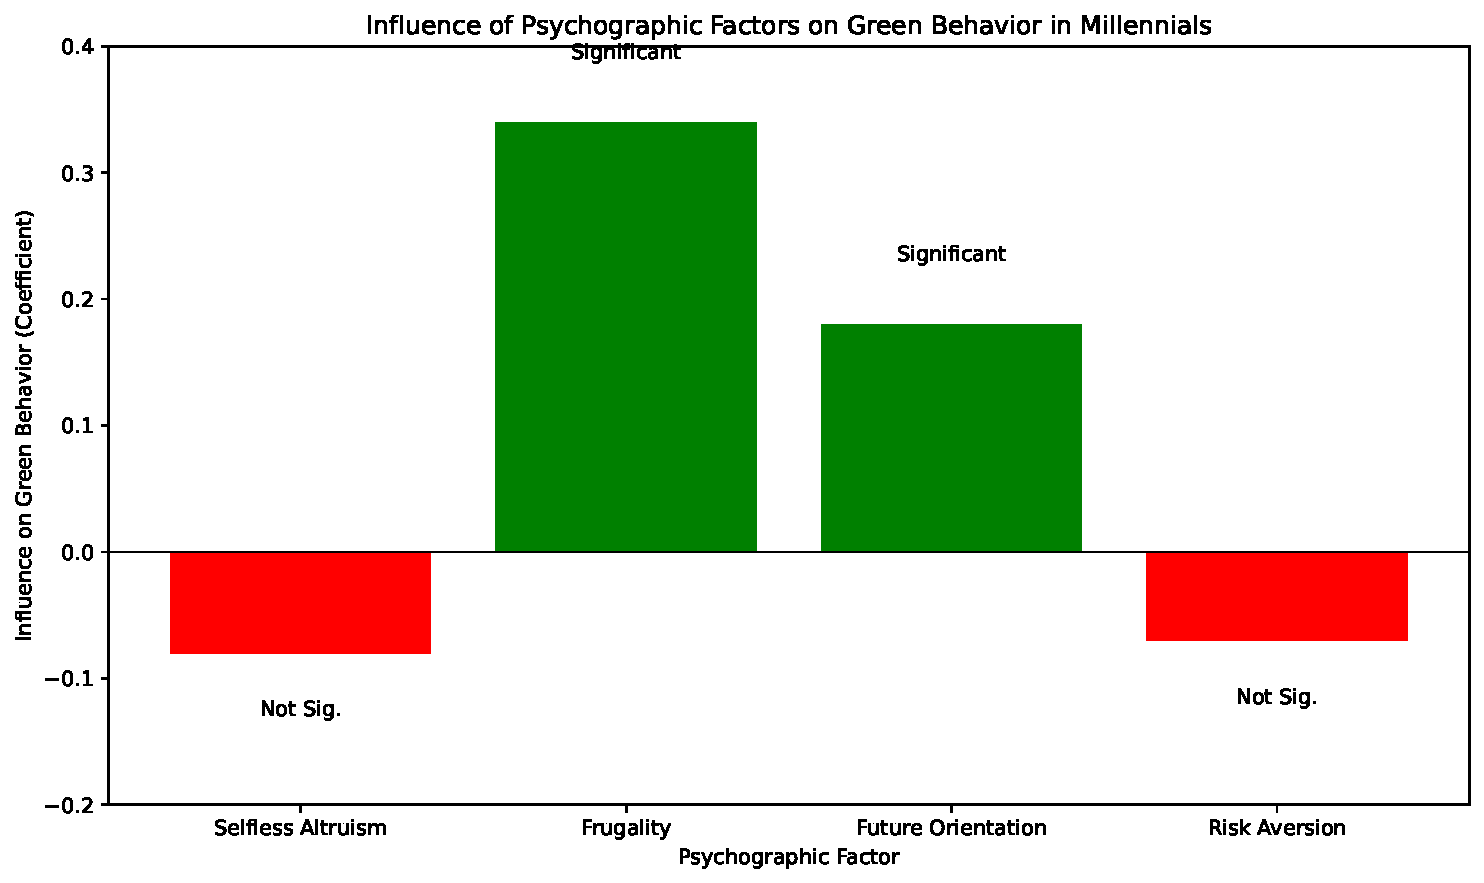
\includegraphics[keepaspectratio]{_thesis-nocite_files/figure-pdf/fig-mil-psych-sust-output-1.pdf}}

}

\caption[Psychological Factors Influencing Millennials to Engage with
Sustainability]{\label{fig-mil-psych-sust}Psychological factors
influencing millennials to engage with sustainability}

\end{figure}%

\subsection{Attitude-Behavior Gap}\label{attitude-behavior-gap}

While people express eco-conscious ideas, it's non-trivial to practice
sustainability in daily life. Translating eco-conscious attitudes into
concrete sustainable actions remains challenging. Empirical evidence
illustrates this gap between intention and behavior. (Park \& Lin, 2020)
positive attitude towards sustainable products does not result in
purchase decisions, shows research of fashion in South Korea. In one
Australian study, green consumers still waste food similarly to the
baseline (McCarthy \& Liu, 2017).

However, changing habits is important if technology alone is not the
solution. (Deyan Georgiev, 2023b) reports only 30\% of people in the
Gen-Z age group believe technology can resolve all environmental
problems. Even with good intentions, (Munro et al., 2023) finds shoppers
who try to shop sustainably often fail to find sustainable product, in a
systemic literature review of 64 papers from South Korea, Australia, the
UK, the US, and elsewhere.

McKinsey's \emph{Talk is Cheap} study underscores the same paradox at
scale: more than 60\% of global consumers say they are willing to pay
extra for sustainable products, yet in reality most wouldn't pay a
premium greater than about 10\% (Freundt et al., 2024). A robust
willingness-to-pay (WTP) literature tells a similar story. A 2021
meta-analysis covering 80 studies finds the average stated premium for
sustainable food products is 29.5\%; however, hypothetical surveys often
overstate WTP relative to real-purchase experiments (S. Li \& Kallas,
2021). In contrast, PwC's 2024 \emph{Voice of the Consumer} survey,
based on 20000 respondents in 31 countries, reports a far more modest
mean sustainability premium of 9.7\% that consumers are willing to pay,
once inflation is factored in (PwC Global, 2024).

In short, people want eco-products but are largely price-sensitive.

\subsection{Sustainability in Taiwan: Garbage Trucks and Digital
Receipts}\label{sustainability-in-taiwan-garbage-trucks-and-digital-receipts}

Musical garbage truck are a success story of the environmental progress
in Taiwan (Helen Davidson \& Chi Hui Lin, 2022). Indeed, they are a
\emph{user interface innovation} and the main way how people in Taiwan
interact with sustainability issues.

The popular narrative about Taiwan recounts the story of the economic
and environmental transformation of the country. In the late 1980s
during the heights of an economic boom Taiwan became famous as the
Taiwanese Miracle (臺灣奇蹟) (Gold, 1986; P.-L. Tsai, 1999). By the
early 1990s another less flattering nickname appeared: \emph{``garbage
island''}, for the piles of trash covering the streets and overflowing
landfills (Ngo, 2020; Rapid Transitions Alliance, 2019). In the two
decades that followed, from 1998 to 2018, Taiwan made progress in
municipal waste management, rising to the status of a world-leader in
recycling (2nd \emph{effective recycling rate} after Germany); in
addition to an effective recycling system, the average waste amount
generated per person by 700g (from 1140g to 400g) per day; nonetheless,
industrial recycling rates were less stellar, standing at 80\% in 2020
and there were unrealized opportunities in using industry 4.0
technologies, such as internet of things (IoT) sensors for better waste
tracking (Bui et al., 2023; C.-Y. Wu et al., 2021).

Progress in sustainability is possible but achieving results takes time
and innovation. (Rapid Transitions Alliance, 2019) credits the Taiwanese
Homemakers United Foundation (財團法人主婦聯盟環境保護基金會) for
initiating the transformation in 1987, suggesting a small group of
people can have an outsized impact on the whole country. Their activity
didn't stop there and (財團法人主婦聯盟環境保護基金會, 2020) recounts a
timeline of their achievements on their website until the present day.

(\emph{{獨家觀察-電子發票年減碳量 相當2,700座大安森林公園}}, 2025)
reports 54.03\% of invoices in Taiwan are digital. Since 2021 digital
receipts are mandatory for all businesses. Taiwan's longstanding receipt
lottery also has specific prizes available only for digital receipts
(\emph{行動支付結合雲端發票 節能減碳最環保{\textbar}經理人}, 2018).
Several other countries, such as Singapore, South Korea, Japan, Sweden,
Italy, Portugal, Brazil, Mexico, have comparable systems in use.

\subsection{Trends in Taiwanese Industry and Online
Shopping}\label{trends-in-taiwanese-industry-and-online-shopping}

In the intensifying competition of online shopping in Taiwan,
(聯合新聞網, 2024) predicts Momo and Coupang will compete for Taiwanese
market leadership, with Coupang increasingly stepping on Shopee's and
MOMO's toes, as per (\emph{順風婦產科 순풍 산부인과 (@Followwindlover)
on {Threads}}, 2024).

Across online and offline, KANTAR reports Taiwan's consumer spending on
fast-moving consumer-goods (FMCG) grew over 5\% in 2024, speeding up
towards the end of the year: +2.5\% in Q1, +4.1\% in Q2, +5.7 \% in Q3
and +9.1\% in Q4, with e-commerce crossing the 20 \% share mark
(traditionally FMCG are purchased physical stores, as convenience stores
are so readily available all over Taiwan) (foodNEXT, 2024; Kantar
Worldpanel, 2024; 動腦Brain.com.tw, 2024; 食力 foodNEXT, 2025).

Taiwan has been on a path of change, striving to become more
sustainable. Between 1970 and 2019, emitting CO\textsubscript{2}eq was
largely a prerequisite for economic growth in Taiwan (T. Chang et al.,
2023). Since the 1990s, Taiwan is a net CO\textsubscript{2}eq exporter
through emissions embedded in the industrial production oriented economy
(R. Huang et al., 2020). Starting in 2023, Taiwan's Financial
Supervisory Commission's (FSC) added ``requirements for Taiwan's
corporates to disclose their carbon emissions,'' (Reformosatw, 2024).
Most recently, the Taiwanese environmental ministry has been cracking
down on illegal waste, with over 70 cases being prosecuted (環境部,
2025).

TIME Magazine and Statista collaborative \emph{``World's Most
Sustainable Companies Of 2024''} includes 17 Taiwanese companies (Alana
Semuels, 2024).

\def\pandoctableshortcapt{World's Most Sustainable Companies}

\begin{longtable}[]{@{}
  >{\raggedleft\arraybackslash}p{(\linewidth - 4\tabcolsep) * \real{0.3288}}
  >{\raggedright\arraybackslash}p{(\linewidth - 4\tabcolsep) * \real{0.3562}}
  >{\raggedleft\arraybackslash}p{(\linewidth - 4\tabcolsep) * \real{0.3151}}@{}}
\caption[World's Most Sustainable Companies]{World's Most Sustainable
Companies; data from (Alana Semuels, 2024).}\tabularnewline
\toprule\noalign{}
\begin{minipage}[b]{\linewidth}\raggedleft
\textbf{Sustainability Rank}
\end{minipage} & \begin{minipage}[b]{\linewidth}\raggedright
\textbf{Company}
\end{minipage} & \begin{minipage}[b]{\linewidth}\raggedleft
\textbf{Score (Out of 100)}
\end{minipage} \\
\midrule\noalign{}
\endfirsthead
\toprule\noalign{}
\begin{minipage}[b]{\linewidth}\raggedleft
\textbf{Sustainability Rank}
\end{minipage} & \begin{minipage}[b]{\linewidth}\raggedright
\textbf{Company}
\end{minipage} & \begin{minipage}[b]{\linewidth}\raggedleft
\textbf{Score (Out of 100)}
\end{minipage} \\
\midrule\noalign{}
\endhead
\bottomrule\noalign{}
\endlastfoot
24 & Delta Electronics & 77.18 \\
63 & Taishin Holdings & 73.50 \\
68 & Fubon Financial & 73.01 \\
80 & Chunghwa Telecom & 71.69 \\
91 & Yuanta Financial Holdings & 70.94 \\
92 & Cathay Financial Holdings & 70.79 \\
108 & Taiwan Mobile & 69.72 \\
200 & First Financial Holding & 64.17 \\
300 & Far EasTone & 60.04 \\
301 & SinoPac Holdings & 60.04 \\
344 & Wistron & 58.44 \\
356 & Acer & 58.02 \\
395 & Nanya Technology & 56.35 \\
409 & InnoLux & 55.82 \\
416 & Wiwynn & 55.67 \\
421 & Taiwan Cement & 55.49 \\
497 & Advantech & 53.14 \\
\end{longtable}

\let\pandoctableshortcapt\relax

Meanwhile, Corporate Knights which has been ranking global sustainable
companies since 2005, including analysis of 7000 public companies with a
revenue over US\$1 billion, only includes TSMC in the top 100 (placed
20th in 2021 and 44th in 2022, dropping out in 2023) and Taiwan High
Speed Rail Corp (THSR) and Giant Manufacturing Co Ltd since 2023
(Corporate Knights, 2024; Staff, 2021). Meanwhile, earth.org's list of
the world's 50 most sustainable companies in 2022, only includes 1
Taiwanese company - TSMC (Earth.Org, 2022).

\begin{figure}

\centering{

\pandocbounded{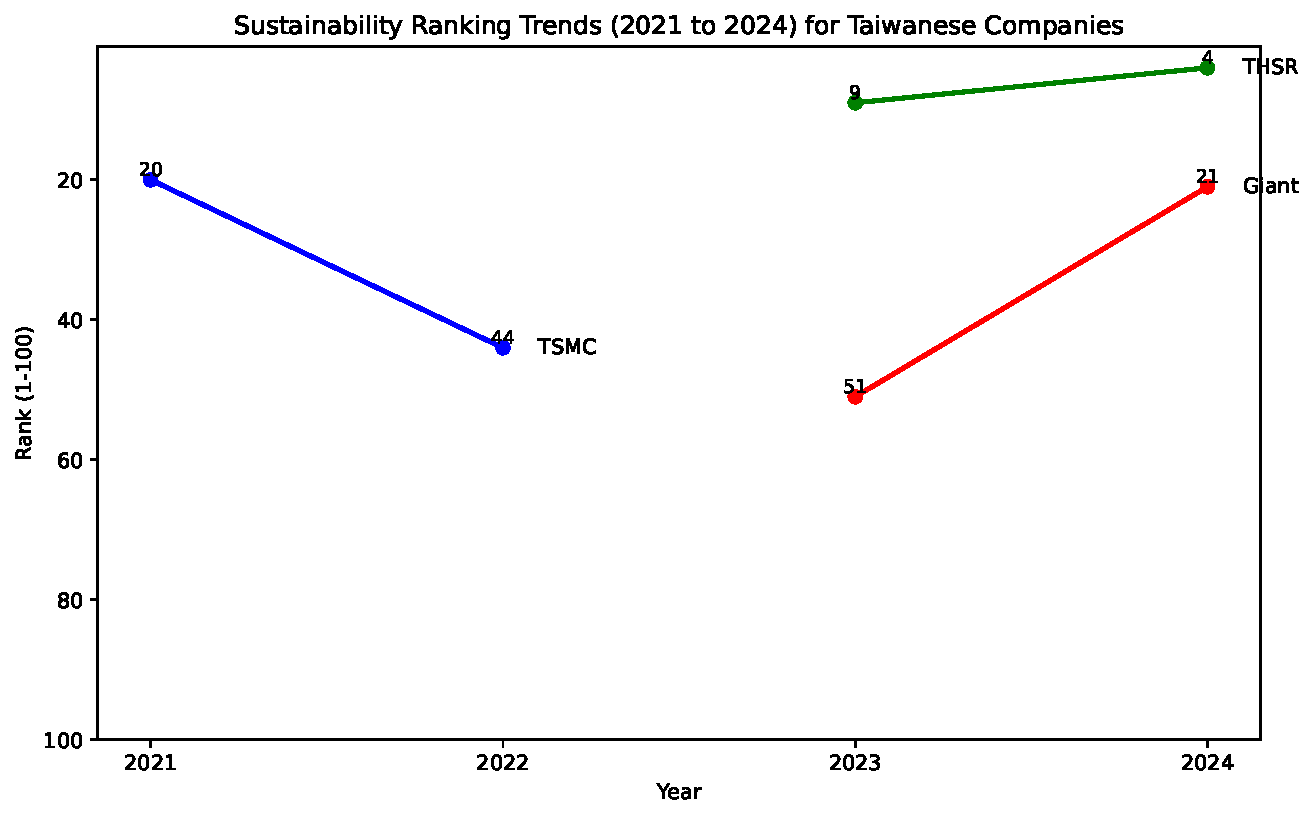
\includegraphics[keepaspectratio]{_thesis-nocite_files/figure-pdf/fig-tw-comp-rank-output-1.pdf}}

}

\caption[Taiwanese Company Ranking]{\label{fig-tw-comp-rank}Taiwanese
Company Ranking}

\end{figure}%

Meanwhile, (Marc Lien, 2022) finds 4 millions British SMEs have no plan
for net-zero transition and (Ware, 2024) adds, British workers lack
skills for green transition, according to a 2024 National Environmental
Services Survey.

\begin{figure}

\centering{

\pandocbounded{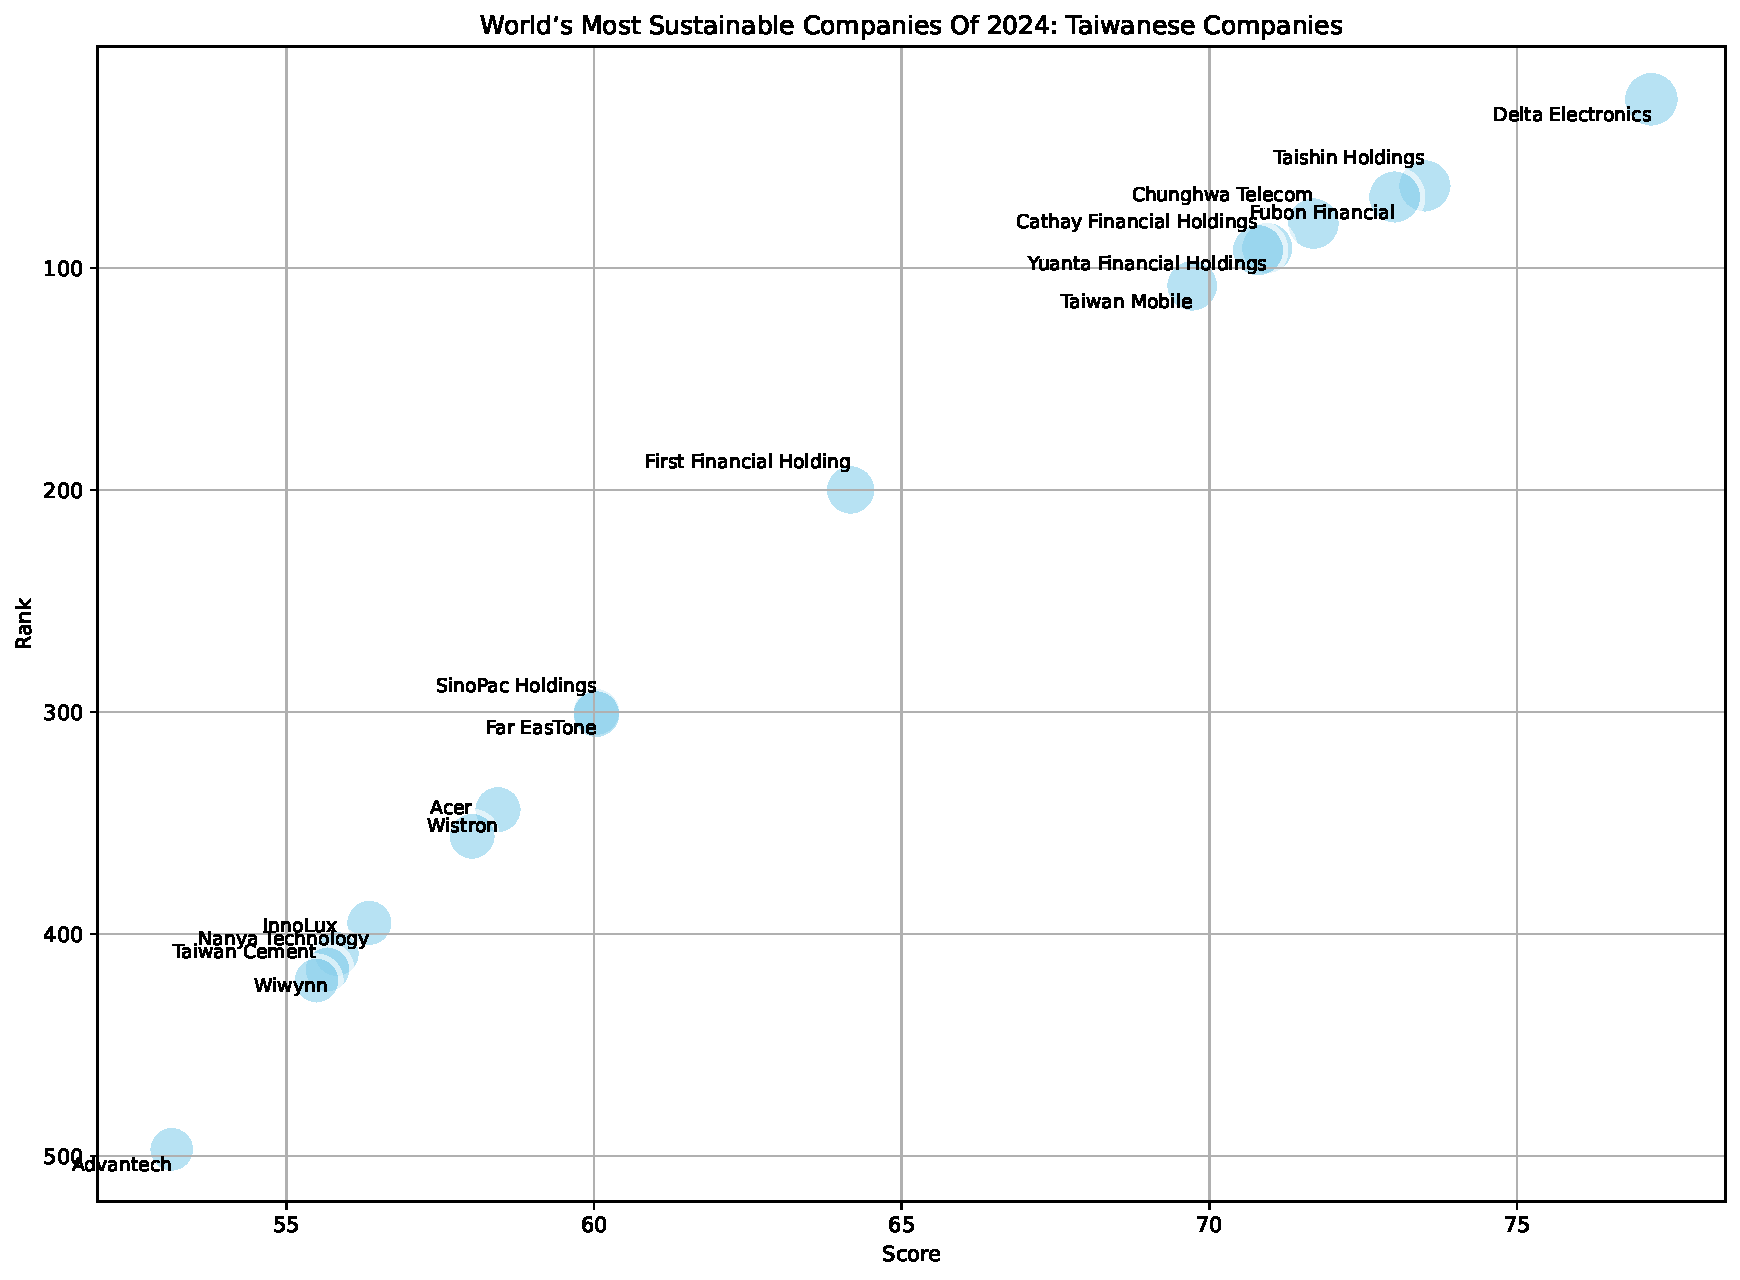
\includegraphics[keepaspectratio]{_thesis-nocite_files/figure-pdf/fig-br-comp-rank-output-1.pdf}}

}

\caption[British Company Ranking]{\label{fig-br-comp-rank}British
Company Ranking}

\end{figure}%

\subsection{Financial Literacy Worldwide and Among Taiwanese
Youth}\label{financial-literacy-worldwide-and-among-taiwanese-youth}

A recent nationwide study (n = 1997) titled Youth Financial Health
Basics (青少年財務健康基礎大調查) jointly conducted by the Taipei Fubon
Bank and the Parent-Child Innovation Center (親子天下教育創新中心)
between February 11 and March 9, 2025 found that over 65\% of secondary
schools incorporated financial-literacy courses into their curricula
however 64\% of Taiwanese youths (aged 15--18) exhibit low confidence
and understanding of financial products and face significant fraud risk,
with nearly 1/5 of the respondents encountering a scam in the past year,
while 18\% suffered actual financial losses (江昭倫, 2025; 陳美君,
n.d.).

\def\pandoctableshortcapt{Taiwanese Financial Product Familiarity}

\begin{longtable}[]{@{}lr@{}}
\caption[Taiwanese Financial Product Familiarity]{Familiarity with
financial products and preferred payment methods, as reported in
(陳美君, n.d.).}\tabularnewline
\toprule\noalign{}
\ul{\textbf{Banking}} & \ul{\% of Respondents} \\
\midrule\noalign{}
\endfirsthead
\toprule\noalign{}
\ul{\textbf{Banking}} & \ul{\% of Respondents} \\
\midrule\noalign{}
\endhead
\bottomrule\noalign{}
\endlastfoot
Have at least one financial account & 80\% \\
\ul{\textbf{Familiarity}} & \ul{\textbf{\% Unfamiliar}} \\
Savings accounts & 70\% \\
Mutual funds & 63\% \\
Stocks & 46\% \\
Deposit accounts & 30\% \\
\ul{\textbf{Payments}} & \ul{\textbf{\% Preference}} \\
Cash & 47\% \\
Family member pays & 47\% \\
EasyCard & 4\% \\
Mobile payments & 1\% \\
\end{longtable}

\let\pandoctableshortcapt\relax

Importantly for designing a financial app, while 80\% of the survey
respondents had received financial education at school, 90\% of the
students deemed the primary learning channel about financial knowledge
to be on social media; and only 15\% remember to have learned about
credit-card usage (江昭倫, 2025).

In a much older study, (I-Cheng Yeh, 2009) analysed usage data from
30,000 credit-card clients at an undisclosed major Taiwanese bank to
predict next-month defaults, using 6 data-mining techniques including
ANNs (AI Neural Networks) (Yeh \& Lien, 2009). Because of the age of the
study there's no Gen-Z data. People aged 18-26 at the time would be
Millennials or Gen-X by now. the data was donated by (Yeh, 2016) and
roughly 1 in 5 credit card clients (22.1\%) of the dataset defaulted on
their payment in the next month. Among the 9,618 clients aged 18--29 at
the time of the study, 2,197 defaulted on their next‐month payment,
yielding a default rate of 22.8\%, slightly higher than the overall
average. Meanwhile, among the 5,127 clients aged 18--26, 1,285
defaulted, yielding a rate of 25.1\%, considerable higher than their
older counterparts. Finally, among the 1,558 clients aged 18--23, 430
defaulted, a rate of 27.6\%, pointing to a trend of younger people
having higher default rates.

A over-the-phone study (n = 3000) conducted in 2022, found Taiwanese
savings habits to have polarized, with over 60\% either having no
savings whatsoever or saving more than 1/2 of their annual income; 27\%
of respondents reported total savings below NT\$40,000; young adults'
(aged 20--29) were the only group whose financial risk worsened, with
43\% of the respondents having extremely low financial literacy,
described as 金融文盲 (near ``financial illiterate'') (中央社, 2022).

\def\pandoctableshortcapt{Financial Literacy Data from Phone Interviews}

\begin{longtable}[]{@{}
  >{\raggedright\arraybackslash}p{(\linewidth - 8\tabcolsep) * \real{0.5811}}
  >{\raggedleft\arraybackslash}p{(\linewidth - 8\tabcolsep) * \real{0.1351}}
  >{\raggedleft\arraybackslash}p{(\linewidth - 8\tabcolsep) * \real{0.0946}}
  >{\raggedleft\arraybackslash}p{(\linewidth - 8\tabcolsep) * \real{0.1081}}
  >{\raggedleft\arraybackslash}p{(\linewidth - 8\tabcolsep) * \real{0.0811}}@{}}
\caption[Financial Literacy Data from Phone Interviews]{Financial
literacy data from phone interviews, as reported in (中央社,
2022).}\tabularnewline
\toprule\noalign{}
\begin{minipage}[b]{\linewidth}\raggedright
Financial Literacy Among Taiwanese (2020)
\end{minipage} & \begin{minipage}[b]{\linewidth}\raggedleft
Very Low
\end{minipage} & \begin{minipage}[b]{\linewidth}\raggedleft
Low
\end{minipage} & \begin{minipage}[b]{\linewidth}\raggedleft
Medium
\end{minipage} & \begin{minipage}[b]{\linewidth}\raggedleft
High
\end{minipage} \\
\midrule\noalign{}
\endfirsthead
\toprule\noalign{}
\begin{minipage}[b]{\linewidth}\raggedright
Financial Literacy Among Taiwanese (2020)
\end{minipage} & \begin{minipage}[b]{\linewidth}\raggedleft
Very Low
\end{minipage} & \begin{minipage}[b]{\linewidth}\raggedleft
Low
\end{minipage} & \begin{minipage}[b]{\linewidth}\raggedleft
Medium
\end{minipage} & \begin{minipage}[b]{\linewidth}\raggedleft
High
\end{minipage} \\
\midrule\noalign{}
\endhead
\bottomrule\noalign{}
\endlastfoot
Overall financial literacy & 43.2\% & 34.9\% & 19.4\% & 2.5\% \\
Understanding products \& services & 34.0\% & 38.6\% & 23.1\% & 4.3\% \\
Confidence using products \& services & 30.0\% & 26.8\% & 37.6\% &
5.6\% \\
Seeking financial advice & 71.0\% & 3.2\% & 17.8\% & 8.0\% \\
Personal money management & 21.8\% & 42.9\% & 28.4\% & 6.9\% \\
\end{longtable}

\let\pandoctableshortcapt\relax

The Taiwanese Financial Literacy \& Education Association 財金智慧FINLEA
is a non-profit with a stated goal of enhancing financial literacy among
Taiwanese. Their longitudinal study, with the latest survey conducted in
2022 (n = 2014; 1055 high-school; 959 university) rated financial
literacy among all youths 56.3 out of 100 (53.8 in 2016 and 56.7 in
2007), always below the benchmark score of 60, with high school and
vocational students averaging 49.26 and university students somewhat
higher averaged 64.03 score (網軟股份有限公司, n.d.).

\def\pandoctableshortcapt{Taiwanese FINLEA Longitudinal Study}

\begin{longtable}[]{@{}
  >{\raggedright\arraybackslash}p{(\linewidth - 2\tabcolsep) * \real{0.6761}}
  >{\raggedleft\arraybackslash}p{(\linewidth - 2\tabcolsep) * \real{0.3239}}@{}}
\caption[Taiwanese FINLEA Longitudinal Study]{Latest report from the
財金智慧FINLEA longitudinal study (網軟股份有限公司,
n.d.).}\tabularnewline
\toprule\noalign{}
\begin{minipage}[b]{\linewidth}\raggedright
Knowledge Gap (2022)
\end{minipage} & \begin{minipage}[b]{\linewidth}\raggedleft
\% Unaware
\end{minipage} \\
\midrule\noalign{}
\endfirsthead
\toprule\noalign{}
\begin{minipage}[b]{\linewidth}\raggedright
Knowledge Gap (2022)
\end{minipage} & \begin{minipage}[b]{\linewidth}\raggedleft
\% Unaware
\end{minipage} \\
\midrule\noalign{}
\endhead
\bottomrule\noalign{}
\endlastfoot
Unsure that employers must contribute to the labor pension (and
individuals can voluntarily contribute) & 68\% \\
Unsure which deductions (income tax, labor insurance, health insurance)
reduce take-home pay & 66\% \\
Unsure how education level affects starting salary & 61\% \\
Unaware of methods to lower loan interest rates & 59\% \\
Cannot identify which auto insurance covers vehicle damage & 55\% \\
Unable to judge which life-insurance need is greatest & 51\% \\
Uncertain how to choose investment tools for maximum lifetime returns &
63\% \\
Unaware that business tax makes purchases more expensive & 61\% \\
\end{longtable}

\let\pandoctableshortcapt\relax

財金智慧FINLEA does publish online videos targeted at young people,
however as of early 2025, they only have around 1000 subscribers on
YouTube (財金智慧FINLEA, 2020). Meanwhile, the Taiwanese cryptocurrency
influencer Mr Block has over 100000 YouTube subscribers (mrblock
區塊先生, 2025).

\begin{figure}[H]

{\centering 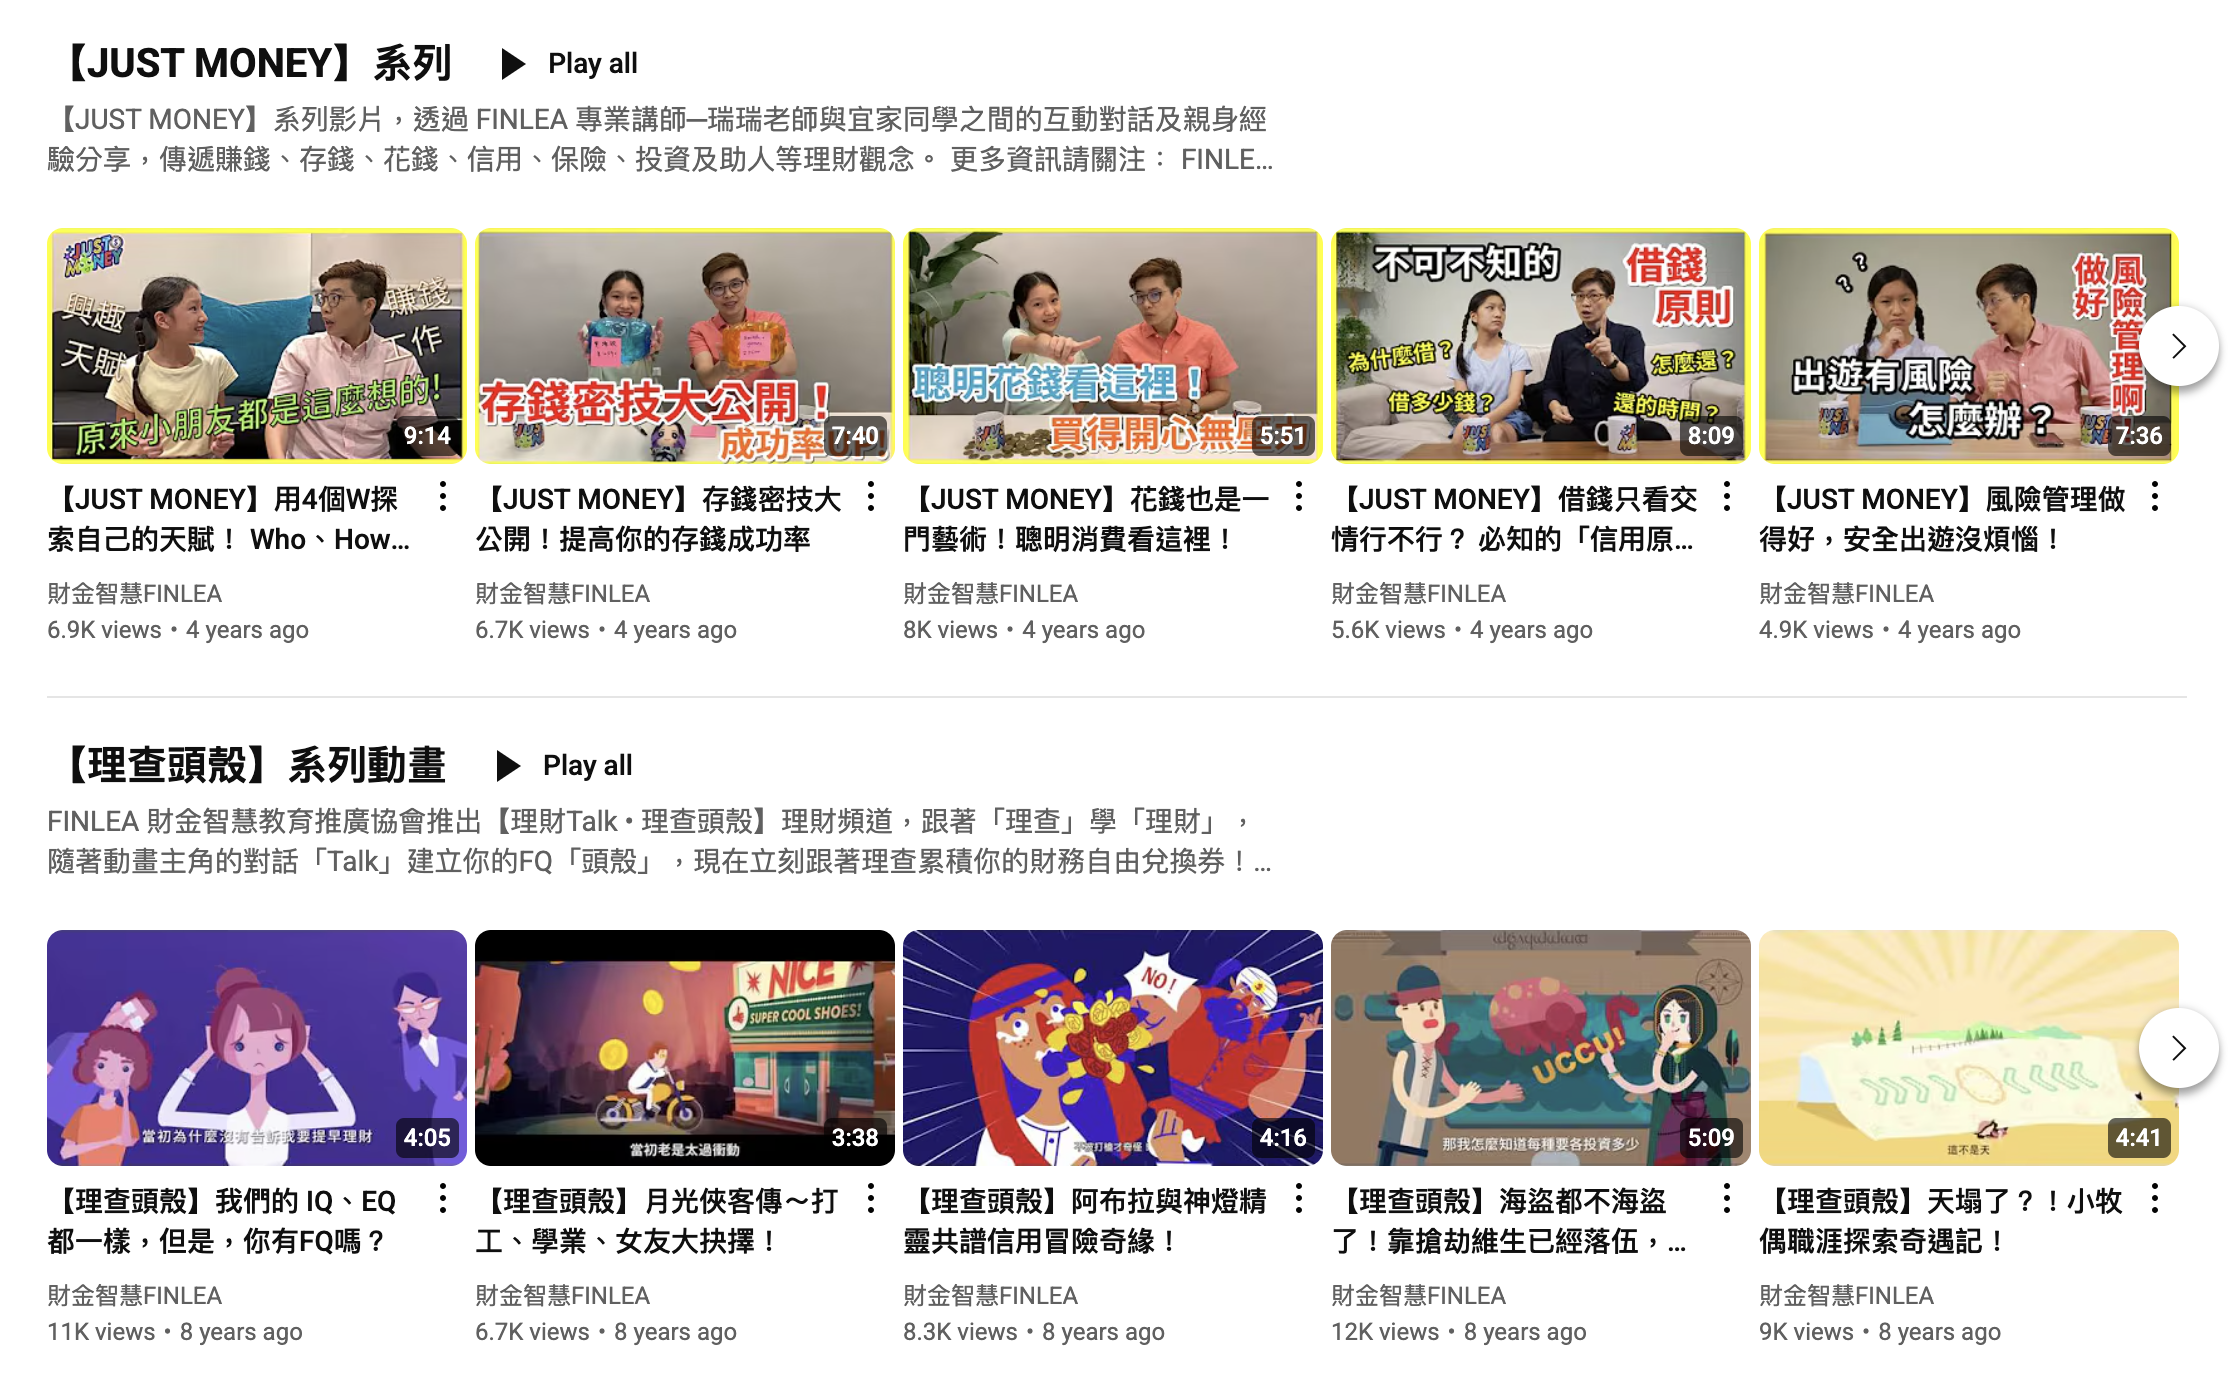
\includegraphics[width=1\linewidth,height=\textheight,keepaspectratio]{./images/college/taiwan-financial-literacy-youtube.png}

}

\caption{財金智慧FINLEA YouTube Channel}

\end{figure}%

Internationally, there's evidence young people have money. In the United
States, the combined annual consumer spending of Gen-Z and Millennials
was over \$2.5 Trillion in 2020 (YPulse, 2020). Over the decade from
2020 to 2030, in the U.S., UK, and Australia, Millennials are projected
to inherit \$30 Trillion USD from their parents (Calastone, 2020).
(Steverman, 2022) puts the inheritance figure between 2022-2045 at an
higher \$73 Trillion USD. There's also some evidence of investment
interest, however with a large geographic variance. According to a
(Calastone, 2020) study (n = 3000) surveying people in the millennial
age group between ages 23 and 35 in Europe (UK, France, Germany),
U.S.A., Hong Kong, and Australia, 48\% of respondents located in Hong
Kong owned financial securities (such as stocks) while the figure was
just 10\% in France.

\def\pandoctableshortcapt{Millennial Investors}

\begin{longtable}[]{@{}ll@{}}
\caption[Millennial Investors]{Data from millennial investors
(Calastone, 2020).}\tabularnewline
\toprule\noalign{}
Place of Comparison & Financial Security Ownership \\
\midrule\noalign{}
\endfirsthead
\toprule\noalign{}
Place of Comparison & Financial Security Ownership \\
\midrule\noalign{}
\endhead
\bottomrule\noalign{}
\endlastfoot
Hong Kong & 48\% \\
France & 10\% \\
& \\
\end{longtable}

\let\pandoctableshortcapt\relax

\subsection{Social Media, Trends, Memes, and Youth
Empowerment}\label{social-media-trends-memes-and-youth-empowerment}

The term ``meme,'' first coined by Richard Dawkins in 1976 in his book
``The Selfish Gene'' to describe units of cultural evolution, analogous
to that of biological evolution, which may evolve by natural selection,
and now encompasses internet artifacts and even stocks. Beyond mere
entertainment, memes have emerged as an academic discipline, where memes
are sampled, coded, and analysed from cultural and ethical viewpoints,
among others (Zidani \& Miltner, 2022). (Peters-Lazaro et al., 2020)
argues memes are no merely jokes but tools for communal critique and
collective visioning. suggesting that Taiwanese Gen-Z memes scaffold
deeper conversations about consumerism, climate action, and social
change. Memes from daily life, business to war, are relevant to
penetrating through the noise of the web.

In Taiwan, homegrown memes may start with global templates but quickly
take on a local flavor. (劉芸嘉, 2024)'s 2021 study of 150 Taiwanese
memes written in Mandarin shows most rely on friendly and indirect
humor: inside jokes and wordplay that bond peers together.
(朱映潔(Ying-Chieh Chu), 2021) surveyed 737 Taiwanese Facebook users and
discovered that a meme's funniness, shareability, and shock value
``hellish gags'' (地獄梗) drive people to post it for social approval.
(胡綺珍, 2024) collected 217 ``tired of life'' / ``I'm just trash'' meme
texts from Instagram and PTT, then interviewed 13 Gen-Z enthusiasts,
revealing how self-deprecating jokes help Gen Z cope with stress, feel
part of a group, and quietly push back against social pressure. Memes
have a long history, and even almost a decade ago in 2016, a casual news
comment---like the ``canoing man'' (泛舟哥) remark during a typhoon
exploded into LINE stickers and PTT threads, proving that Taiwanese can
transform everyday media moments into collective satire or
tongue-in-cheek commentary (黃意能 \& 黃曉琪, 2016).

Internationally, the sustainability-focused topics ``underconsumption''
and ``deinfluencing'' were trending on TikTok in 2024 however have since
subdued (Fares et al., 2024; TikTok, 2024b, 2024a). While this
particular trend may be over, memes still hold potential for
communicating about sustainability to young Taiwanese. Still, looking at
older international data, (Zannettou et al., 2018) built a large-scale
machine-learning pipeline to trace the origin of memes in the US, with
160M images and 2.6B posts within about 1 year (July 2016-2017) from
Twitter, Reddit, 4chan and Gab, finding that often memes originate from
fringe communities and then spread across mainstream media, highlighting
how fringe communities can be surprising impactful.

In Taiwan, Internet usage among young people is nearly universal, with
over to 98\% of 18--29 (roughly Gen-Z) year‐olds reporting they have
gone online at least once recently, and close to 96\% of respondents
aged 18-29 used some form of social media (財團法人台灣網路資訊中心 \&
台灣資訊社會研究學會, 2023).

\def\pandoctableshortcapt{Taiwanese Internet Usage Statistics}

\begin{longtable}[]{@{}lll@{}}
\caption[Taiwanese Internet Usage Statistics]{Taiwanese Internet Usage
Statistics; data from (財團法人台灣網路資訊中心 \& 台灣資訊社會研究學會,
2023).}\tabularnewline
\toprule\noalign{}
Metric & 18--29 & 30--39 \\
\midrule\noalign{}
\endfirsthead
\toprule\noalign{}
Metric & 18--29 & 30--39 \\
\midrule\noalign{}
\endhead
\bottomrule\noalign{}
\endlastfoot
Daily Internet usage & 98.79 \% & 98.40 \% \\
Overall social-media usage & 95.98 \% & 94.84 \% \\
TikTok usage & 33.03 \% & 24.28 \% \\
\end{longtable}

\let\pandoctableshortcapt\relax

(林高賢, 2024) analysed (n = 1175) Taiwanese high school students,
mostly aged Gen-Z, finding that Instagram (IG) dominates, used by close
to 85\% percent of the respondents; they use IG for about 2 hours per
day, 5-6 days per week; moreover, respondents often feel anxious (1-2
days per week), and anxiety correlates with several motivations of using
IG, such as recording life moments, documenting travel, food, and
fitness with photos, was tied to higher anxiety, possibly related to the
photo-centric self-presentation on Instagram, why can be theorized to
heighten sensitivity to feedback and criticism. In contrast, (陳思凝,
2023) conducted a survey of 458 Taiwanese Gen Z Instagram users, finding
that higher Instagram use intensity is directly associated with greater
online subjective well-being; however, intense use also leads to
information overload and social comparison, which induce social media
fatigue and in turn erode well-being; moreover, users' perceived
intimacy with the platform amplifies the link between use intensity and
social comparison frequency. An online survey by (廖柏雅, 2024) (where
the Gen-Z cohort n = 125) found respondents to be highly motivated by
social and entertainment use; the user's fear of missing out (FoMO) was
found to be related to the motive; e.g.~people with social and
entertainment drives experience greater FoMO than those motivated
primarily by information seeking. (Lasnik, 2018) surveys college
students at the National Dong Hwa University in Hualian (n = 300, a mix
of Taiwanese and international students), using the Liebowitz Social
Anxiety Scale (LSAS) and Taijin Kyofusho Scale (TKS) as research
instruments, finding Taiwanese students ranked higher on the Taijin
Kyofusho, suggesting the fear of offending or disturbing others is
stronger among local students.

A large-scale (n = 2075) representative face-to-face survey among people
aged 18 to 93 years in Taiwan (no age-based categorization was published
for Gen-Z specifically), found that in general sharing one's thoughts
online (known academically as ``self-disclosure'') boosts perceived
social support and significantly boosts bonding and bridging social
capital, which increases life satisfaction and lowers loneliness (樊一寧
et al., 2024). Conversely, in Japan, while not directly comparable,
Gen-Z reports wanting privacy and 75\% feel others overshare on social
media and 49 percent were concerned about their personal data (McKinsey
\& Company, 2022).

\subsection{AI Use Among Taiwanese
Students}\label{ai-use-among-taiwanese-students}

A survey of college students in March 8--10, 2023 at the Chung Yuan
Christian University (n = 983) in Taoyuan (Northern Taiwan), yielded the
following results: 66\% of the students had used ChatGPT, with the top
use cases being summarization (31\%), translation of articles (28\%),
and writing reports (24\%) (CYCU, 2023; 許維寧, 2023). However, in terms
of AI adoption, this data can be considered out-dated. ChatGPT was first
released to the public on November 30, 2022, so the students had had
only about 3 months to try it out (OpenAI, 2022). At the time, the
GPT-3.5 model was available; the revolutionary GPT‑4 was released to the
public on March 14, 2023, (OpenAI, 2023).

In a more recent large-scale survey focusing on AI literacy administered
to the general public (n = 2174) found that only 26\% of the respondents
had used ChatGPT in the past 3 months (in comparison with the 25\% from
a similar survey administered in the previous year); younger people had
higher usage patterns, 53\% for 18-29 and 37\% 30-39; meanwhile, 69\% of
respondents believed they could tell the difference between AI-generated
and non-AI content and 73\% supported some type of government
regulations for AI (HakkaNews, 2024).

A Chinese study from two authors at the Minzu University and Beijing
Normal University reports they recruited anonymous Taiwanese college
students (n = 916) on the Chinese Credamo platform from the Taiwanese
IP-space (ChatGPT is blocked in Mainland China, Macau, and Hong Kong) to
compare ChatGPT vs.~Google for academic use among Taiwanese students:
their findings show a clear preference for ChatGPT overall, which
students deemed more flexible (meanwhile some older students still
preferred Google) and Random Forest and LightGBM-based modeling
predicted tool choice by three main factors: 1) GenAI fluency,
2)awareness of GenAI hallucinations, and 3) user age; their
recommendations include 1) support critical-thinking among users, and 2)
design hybrid chat+search user interfaces with higher reliability
(Kelly, 2024; Qiao \& Lee, 2024; M. Zhang \& Yang, 2024). In the US, an
older study of young adults (Millennials at the time) highlights how
they \emph{``use Google as a reference point for ease of use and
simplicity'',} (Kate Moran, 2016). The web now has several generations
of native users, and some older usage patterns which older digital
natives are used to, may take time to change.

In Sweden, a large-scale (n = 5894) survey across several Swedish
universities showed college students' attitudes towards AI assistants
(ChatGPT was by far the most prevalent app, 95 \% of respondents had
heard of ChatGPT and 35 \% used it regularly); 55.9\% held a positive
attitude toward AIs; integrity was a hotly debated question, 62\%
calling AI use in exams ``cheating,'' but 60\% rejecting an outright
ban, and 58\% saying it doesn't violate the purpose of education (Stöhr
et al., 2024).

\begin{figure}

\centering{

\pandocbounded{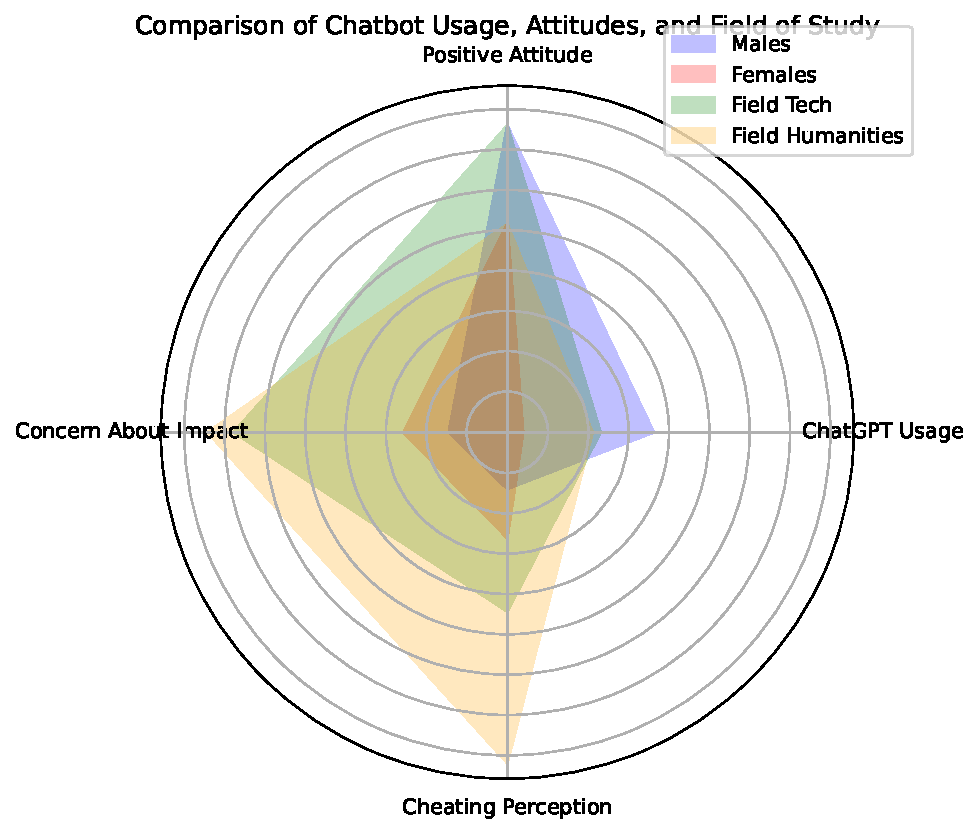
\includegraphics[keepaspectratio]{_thesis-nocite_files/figure-pdf/fig-college-chatbot-output-1.pdf}}

}

\caption[Swedish College Students' Attitudes Towards AI
Assistants]{\label{fig-college-chatbot}Swedish College Students'
Attitudes Towards AI Assistants}

\end{figure}%

\newpage

\section{Sustainability}\label{sustainability}

\begin{figure}[H]

{\centering \pandocbounded{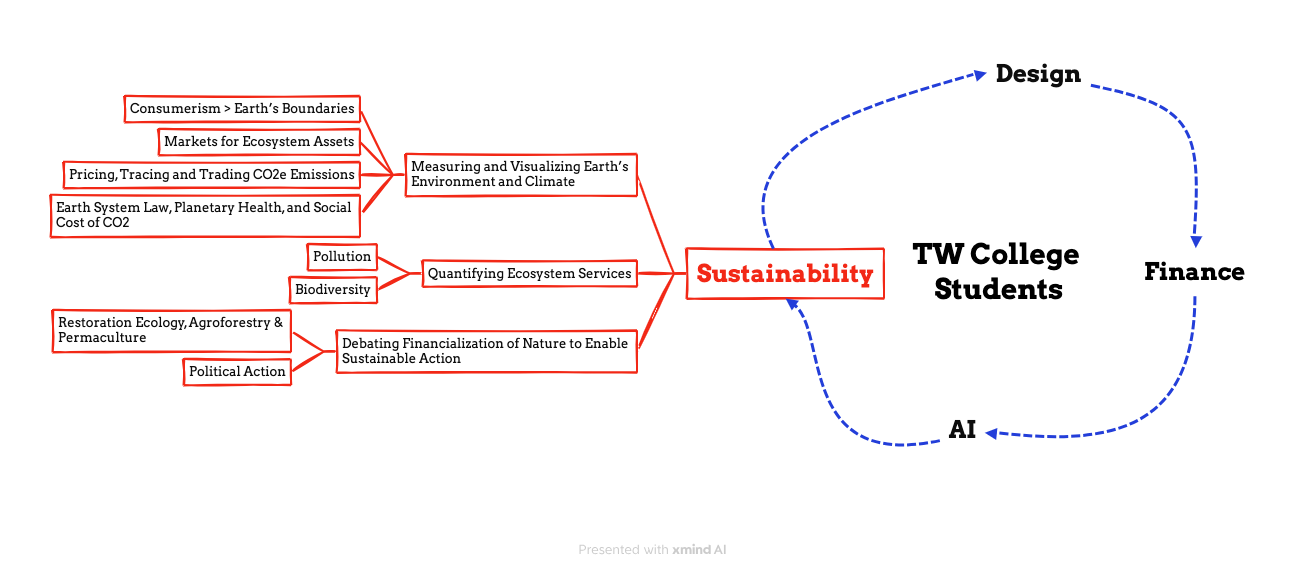
\includegraphics[keepaspectratio]{./images/sustainability/abstract-sustainability.png}}

}

\caption{Visual abstract for the sustainability chapter}

\end{figure}%

\subsection{The Roots of Sustainability in
Environmentalism}\label{the-roots-of-sustainability-in-environmentalism}

\emph{``Nachhaltigkeit''} - \emph{sustainability} in German - was likely
the first use of the concept of preserving natural resources, conceived
by a tax accountant Hannß Carl von Carlowitz in 1713 in his seminal book
on forestry - \emph{Sylvicultura oeconomica -}, referring to the goal of
achieving prudent forest management practices in his native Saxony in
Southeastern Germany, which at the time was under severe
\emph{deforestation} pressure from mining, ship-building and
agricultural production (Gottschlich \& Friedrich, 2014; Hannß Carl von
Carlowitz, 1713). This particular field of sustainability study is now
known as \emph{sustainable yield of natural capital}. The
\emph{principal} of the natural resource being managed, such as in
fishing and forestry, shouldn't be over-harvested in order to maintain
\textbf{\emph{ecosystem services}} - a contemporary term from the theory
of \emph{natural capital}, referring to benefits humans receive from the
stock of world's natural resources (Peter Kareiva et al., 2011).

Defining sustainability perhaps more poetically, the American wildlife
ecologist Aldo Leopold proposed the idea of \emph{land ethics} in 1972
as \emph{``{[}a{]} thing is right when it tends to preserve the
integrity, stability, and beauty of the biotic community. It is wrong
when it tends otherwise''} in his landmark work \emph{A Sand County
Almanac} (Leopold, 1972). In a similar vein, the 1987 United Nations'
Brundtland Report titled ``\emph{Our Common Future''} defined
\emph{sustainable development} as \emph{``Development that meets the
needs of the present without compromising the ability of future
generations to meet their own needs''} (World Commission on Environment
and Development, 1987). Given these varied ideas for over 300 years, I
believe some percentage of people have been concerned with our planet's
natural environment and its preservation already for centuries. Yet, it
is only in the last 100 and so years that human activities have begun to
affect Earth's systems on a previously unseen scale - termed
\emph{Anthropocene} -, necessitating a deeper understanding of
human-nature interactions, such as in the case of climate change, which
is rapidly changing the face of our living environments.

\subsection{Measuring and Visualizing Earth's Climate
Systems}\label{measuring-and-visualizing-earths-climate-systems}

Studies of Earth's climate go back for over 200 years, starting with
Alexander von Humboldt, the founder of climatology, who revolutionized
cartography by inventing the first \emph{isothermal maps} in 1816; these
maps showed areas with similar temperature, variations in altitude and
seasons in different colors (Honton, 2022) now available as 3D computer
models (\emph{Alexander von {Humboldt}'s Original Isotherms Circa 1838},
2023). Already in 1896, the Nobel Prize winner Svante Arrhenius first
calculated how an increase in CO\textsubscript{2} levels could have a
warming effect on our global climate (Anderson et al., 2016; Wulff,
2020). In 1938, Guy Stewart Callendar was the first scientist to
demonstrate the warming of Earth's land surface as well as linking the
production of fossil fuels to increased CO\textsubscript{2}e and
changing climate (Hawkins \& Jones, 2013). Early scientists pioneered
climate modeling by calculating the first climate interactions which
precede today's complex computer-based \emph{Earth System Models (ESMs)}
that integrate the various Earth systems and cycles run on
supercomputers (Anderson et al., 2016).

\begin{figure}[H]

{\centering 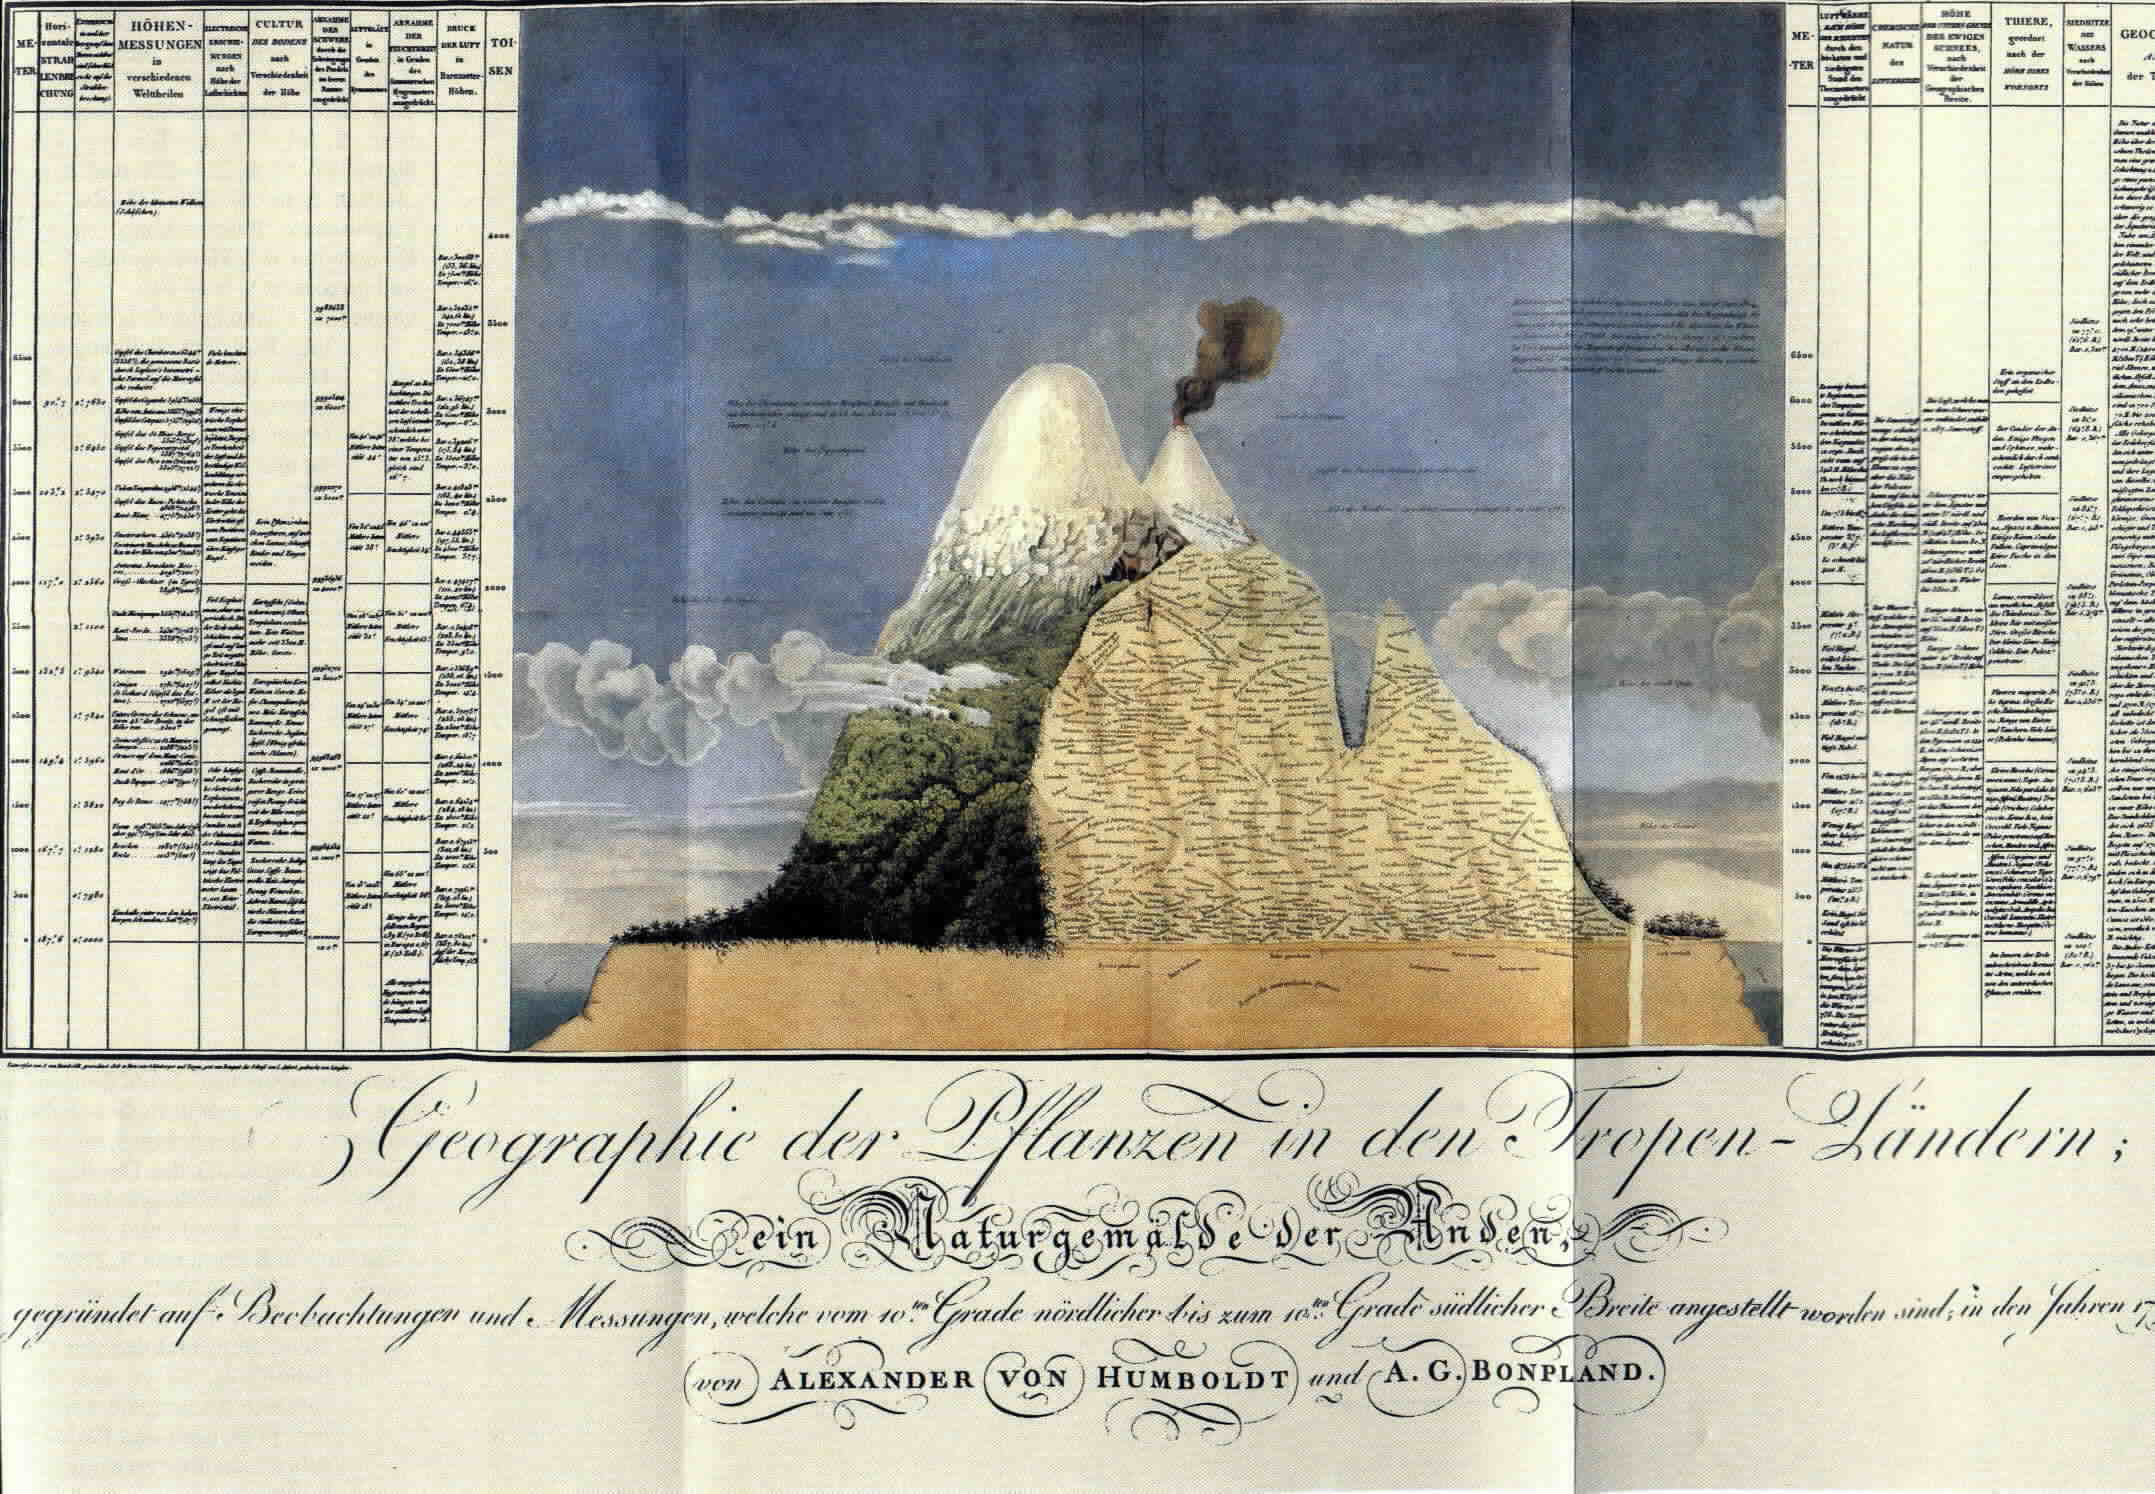
\includegraphics[width=1\linewidth,height=\textheight,keepaspectratio]{./images/sustainability/humboldt.jpg}

}

\caption{Humboldt's Naturgemälde, early data visualization of ecology,
rain, temperature, elevation, etc}

\end{figure}%

Environmental activists have been calling attention to global warming
for decades, yet the world has been slow to act (McKibben, 1989). While
the scientific case for human-induced climate change was building, it
took 120 years after Arrhenius' calculations, until the Paris Climate
Agreement in 2016, that countries came to an agreement on non-binding
targets on keeping CO\textsubscript{2} levels 1.5 °C below
pre-industrial levels (defined as 1850--1900)(United Nations, 2016).
Even though awareness of Earth's warming climate was growing ever
stronger, the CO\textsubscript{2} emissions kept rising too. The
hockey-stick growth of CO\textsubscript{2} concentration since the
industrial revolution is clear in the data from 1958 onward, following a
steady annual increase, called the \emph{Keeling Curve} (Keeling \&
Keeling, 2017). Written records of global temperature measurements are
available starting from the 1880s, when temperatures began to be
documented in ship logs (Brohan et al., 2012). Finally, although perhaps
less accurately, temperature estimations from tree-trunks allow some
comparisons with the climate as far back as 2000 years ago (Rubino et
al., 2019).

April 2025 was Earth's 2nd-warmest April on record, with global
temperatures reaching 1.32°C above the 20th-century average, driven by
persistent El Niño conditions and record-high ocean temperatures
(Masters, 2025). This warming aligns with growing concerns about Earth's
energy imbalance, which recent satellite data suggest has nearly doubled
since 2005; more heat is being trapped in the climate system than is
being radiated back to space (Mauritsen et al., 2025). Compounding the
issue, 3 key NASA climate satellites responsible for monitoring Earth's
energy budget are nearing the end of their operational life with no
replacement missions currently planned, raising alarms about the
continuity and reliability of future climate data (Harvey, 2025).
Likewise, funding for the Scripps Institute, responsible for the Keeling
Curve, is under threat, according to its caretaker, Ralph Keeling.

The Keeling Curve apparatus measures absorption of infrared light, which
allows one to detect the amount of CO\textsubscript{2}eq in the air. It
also has an advanced calibration system where it makes measurements in
air with a known quantity of gases (Worthington, 2025b).

\begin{figure}

\centering{

\pandocbounded{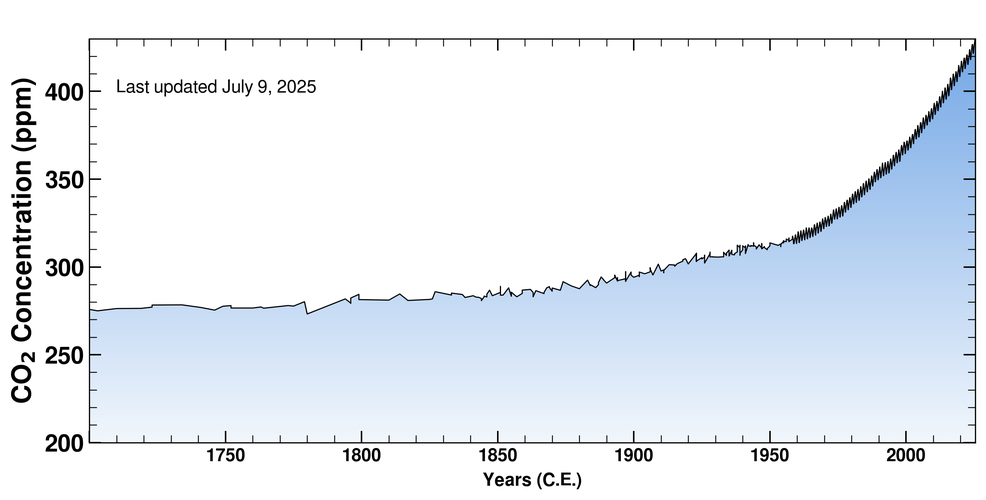
\includegraphics[keepaspectratio]{./images/sustainability/co2-concentration.png}}

}

\caption[Atmospheric CO\textsubscript{2} Concentration
(2025)]{\label{fig-co2-concentration}CO\textsubscript{2} concentration
in the atmosphere as of 2025. Image Credit: Scripps Institution of
Oceanography at UC San Diego.}

\end{figure}%

The latest data from 2023 shows our current world population of 8
Billion people emitted 37.2 gigatonnes (i.e.~billion metric tons) of
CO\textsubscript{2}e per year, the highest emissions recorded in history
(Statista, 2023a). Since 1751, cumulative CO\textsubscript{2}eq
emissions have exceeded 1.5 trillion tonnes globally or when expressed
in CO\textsubscript{2}eq for all green house gases, total historic
emissions would reach roughly 1.7 trillion tonnes CO\textsubscript{2}eq
since the start of the Industrial Revolution.(Global Carbon Budget,
2023; Marvel, 2023). In order to limit global warming to 1.5 °C as
agreed by the world nations in Paris, removal of 5-20 gigatons of
CO\textsubscript{2}e per year would be needed according to reduction
pathways calculated by the Intergovernmental Panel on Climate Change
(IPCC) (UNFCCC. Secretariat, 2022; Wade et al., 2023). Yet, most
countries are missing the mark (Climate Analytics \& NewClimate
Institute, 2023; United Nations Environment Programme, 2023). The
European Union's Copernicus Climate Change Service (C3S) reports 1.5 °C
global warming has already been breached in 2024 temperatures
(\emph{First Time World Exceeds 1.{5C} Warming Limit over 12-Month
Period}, 2024; \emph{World's First Year-Long Breach of Key 1.{5C}
Warming Limit}, 2024). Given the current pace of climate change action,
the G7 countries (Canada, France, Germany, Italy, Japan, United Kingdom,
United States) are heading for 2.7 °C of warming by 2050 (CDP, 2022).

(United Nations Environment Programme (UNEP), 2021) reported as of 2021
updated national climate pledges (NDCs) and other mitigation measures
are projected to lead to a global temperature increase of approximately
2.7°C by 2100, significantly surpassing the Paris Agreement's
aspirational goal to keep global warming below 1.5°C this century;
effective implementation of net-zero emissions pledges could still keep
warming around 2.2°C (approaching the Paris Agreement's goal of below
2°C), if countries cut methane emissions from fossil fuel, waste, and
agricultural sectors, bridging the current emissions gap - and carbon
markets might significantly cut emissions, if they are governed by clear
rules ensuring genuine emission reductions, alongside transparent
systems for monitoring and tracking progress - however, numerous
national climate strategies postpone substantial action until after
2030. A year later, the 2022 Emissions Gap report showed a somewhat
worsening situation, with existing national pledges leading the world
for around 2.8 °C of warming by 2100 (United Nations Environment
Programme, 2022)

Earth's physical systems are very sensitive to small changes in
temperature, which was not understood until the 1970s(McKibben, 2006). A
comprehensive review of evidence from paleoclimate records until current
time, including ocean, atmosphere, and land surface of points towards
substantial climate change if high levels of greenhouse gas emissions
continue, termed by the authors as \emph{climate sensitivity} (Sherwood
et al., 2020). Global warming may lead to the slowing down and complete
stop of the Atlantic meridional overturning circulation (AMOC) which
helps maintain climate stability (Ditlevsen \& Ditlevsen, 2023). Apart
from CO\textsubscript{2}, reduction of other atmospheric pollutants,
such as non-CO\textsubscript{2} greenhouse gases (GHGs) and short-lived
climate pollutants (SLCPs) is required for climate stability (J. Lin et
al., 2022).

(Armstrong McKay et al., 2022a; TED, 2024) warns that climate is not a
linear system, rather there are several non-linear climate tipping
points, where change accelerates: at the current warming ice‐sheet
collapse, permafrost thaw, Amazon dieback and coral‐reef loss are likely
to tip between 1.5 °C and 2 °C, underscoring that the Paris Agreement
range is far from a safe limit. (Armstrong McKay et al., 2022b)
synthesize paleoclimate records, observations, and model projections to
revise and rank both global ``core'' and regional ``impact'' climate
tipping elements by their warming thresholds, visualized in the chart
below.

\begin{figure}

\centering{

\pandocbounded{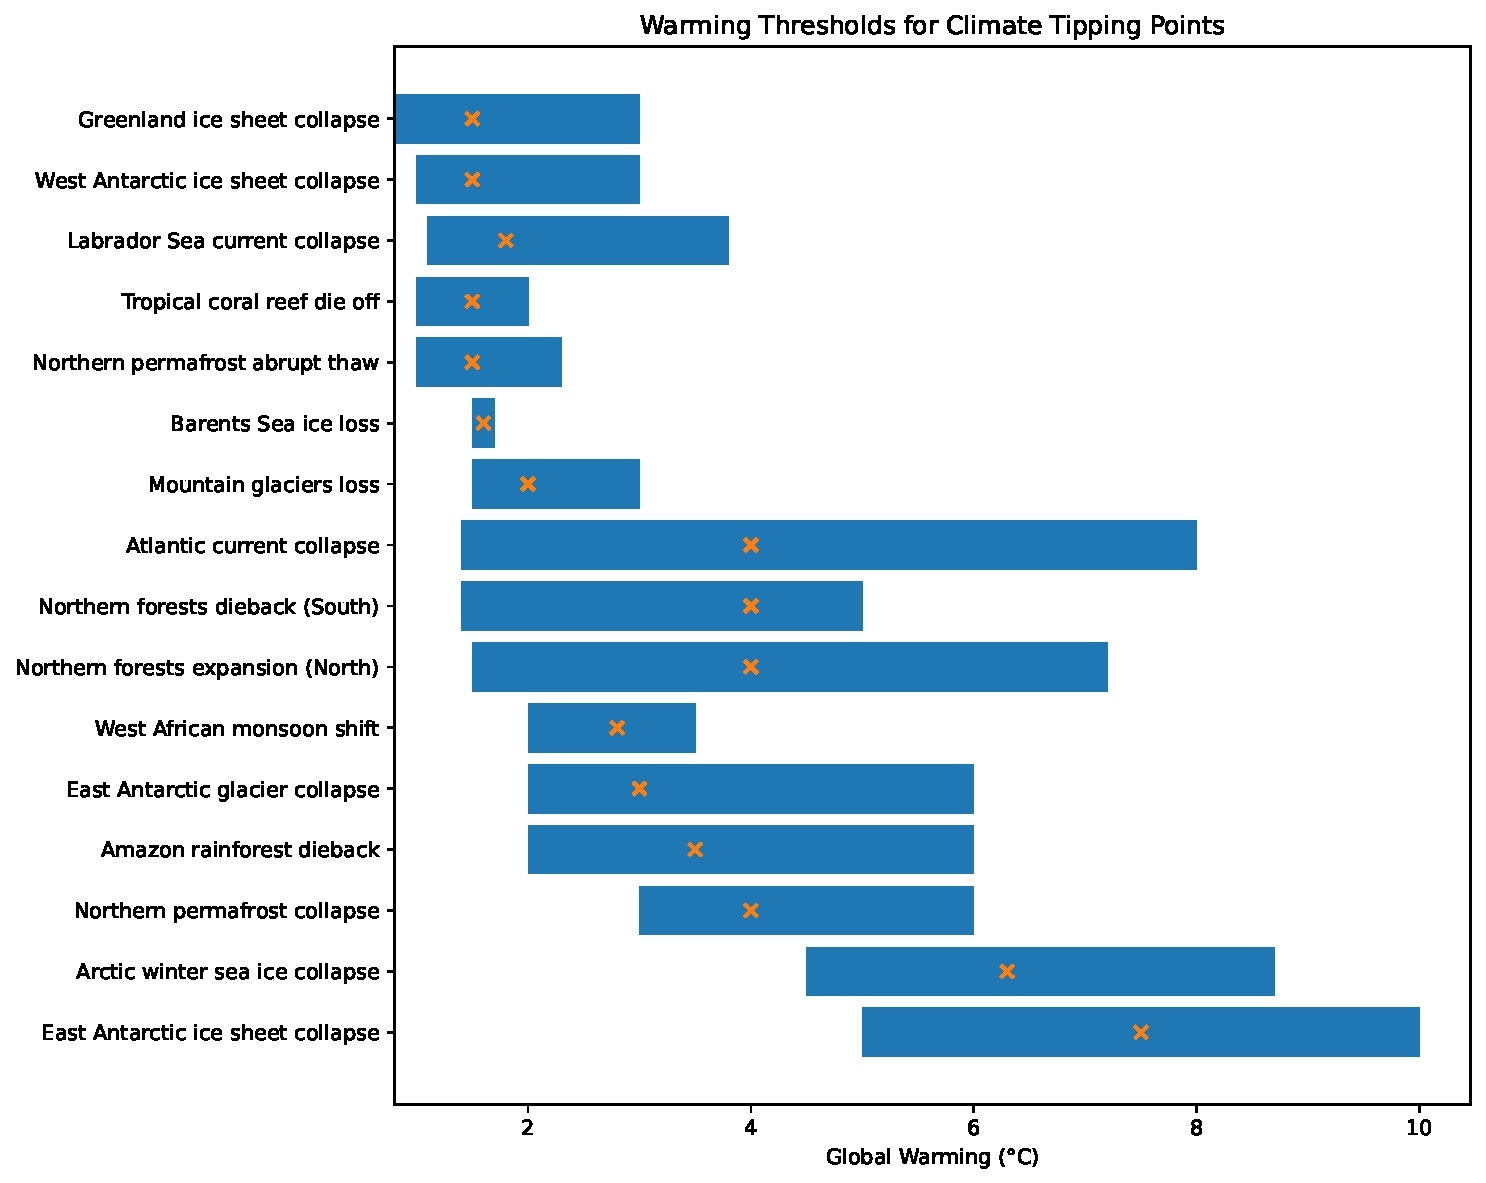
\includegraphics[keepaspectratio]{_thesis-nocite_files/figure-pdf/fig-climate-tip-output-1.pdf}}

}

\caption[Climate Tipping Points]{\label{fig-climate-tip}Climate Tipping
Points}

\end{figure}%

\subsubsection{\texorpdfstring{Measuring CO\textsubscript{2}e
Emissions}{Measuring CO2e Emissions}}\label{measuring-co2e-emissions}

Technology improves and measurements have become more accurate yet
CO\textsubscript{2}e emissions are not yet completely accounted for.
(Crippa et al., 2020) reports the latest figures CO\textsubscript{2}e
from the EU's Emissions Database for Global Atmospheric Research
(EDGAR). The EU Copernicus satellite system reveals new greenhouse
emissions previously undetected (Daniel Värjö, 2022). \emph{Copernicus
Climate Change Service (C3S) provides ``{[}n{]}ear-real time updates of
key global climate variables}''(The Copernicus Climate Change Service,
2024). Using simple python code and freely available images from online
datasets, it's increasingly possible for anyone to detect deforestation,
as in this example of geospatial analysis from Amazon AWS (AWS, 2022; P.
Patel, 2025).

One major cross-cutting category the IPCC tracks separately is LULUCF
(Land Use, Land-Use Change, and Forestry). Depending on whether forests
are being cleared or restored, LULUCF can act as a net greenhouse-gas
source or as a powerful carbon sink that removes CO\textsubscript{2}
from the atmosphere. LULUCF also links to biodiversity protection. (Y.
Chen et al., 2023) looked at the Poyang Lake in China between 2010-2020,
finding ecosystem vulnerability rose by 18\% with human activities
(land-use change, urban expansion, components of LULUCF, also reported
in international media, see (Scarr \& Sharma, 2021) for images) as the
dominant driver, followed by climate factors. (Xie et al., 2021) mapped
pollution sources in 14 vulnerable areas in China, including the Poyang
Lake, and underlined the need for real-time monitoring of ecosystem
health.

Emissions production is highly unequal, with \emph{``{[}t{]}he world's
top 1\% of emitters produce over 1000 times more CO\textsubscript{2}eq
than the bottom 1\%''} (IEA, 2023a). The share of CO\textsubscript{2}
emissions among people around the world is highly unequal across the
world (referred to as \emph{Carbon Inequality}). (Chancel, 2022) reports
``one-tenth of the global population is responsible for nearly half of
all emissions, half of the population emits less than 12\%''.
Information and communications technology (ICT) sector is an example of
carbon inequality, where emerging economies bear 82\% of the emissions,
developed countries gain 58\% of value, of the over 300 million PCs sold
per year (Bajarin, 2022; X. Zhou et al., 2022).

CO\textsubscript{2}e emissions by region (per year), comparing highest
per capita CO\textsubscript{2e} emissions (mostly from oil producers) vs
regional average per capita CO\textsubscript{2} emissions vs total
CO\textsubscript{2} emissions.

\def\pandoctableshortcapt{Regional CO\textsubscript{2} Emissions
Comparison}

\begin{longtable}[]{@{}
  >{\raggedright\arraybackslash}p{(\linewidth - 4\tabcolsep) * \real{0.3889}}
  >{\raggedright\arraybackslash}p{(\linewidth - 4\tabcolsep) * \real{0.3194}}
  >{\raggedright\arraybackslash}p{(\linewidth - 4\tabcolsep) * \real{0.2917}}@{}}
\caption[Regional CO~2~ Emissions Comparison]{CO\textsubscript{2}
Emissions Comparison (Crippa et al., 2020; European Commission. Joint
Research Centre., 2022; Ivanova et al., 2020; Z. Liu et al., 2023; World
Resources Institute, 2020).}\tabularnewline
\toprule\noalign{}
\endfirsthead
\endhead
\bottomrule\noalign{}
\endlastfoot
\textbf{Regional Average Per Capita Emissions (2020)} & \textbf{Highest
Per Capita Emissions (2021)} & \textbf{Highest Total Emissions
(2021)} \\
North America 13.4 CO\textsubscript{2}e tonnes & Palau & China \\
Europe 7.5 CO\textsubscript{2}e tonnes & Qatar & United States \\
Global Average 4.1 CO\textsubscript{2}e tonnes & Kuwait & European
Union \\
Africa and the Middle East 1.7 CO\textsubscript{2}e tonnes & Bahrain &
India \\
& Trinidad and Tobago & Russia \\
& New Caledonia & Japan \\
& United Arab Emirates & Iran \\
& Gibraltar & Germany \\
& Falkland Islands & South Korea \\
& Oman & Indonesia \\
& Saudi Arabia & Saudi Arabia \\
& Brunei Darussalam & Canada \\
& Canada & Brazil \\
& Australia & Turkey \\
& United States & South Africa \\
\end{longtable}

\let\pandoctableshortcapt\relax

\emph{Scoping} CO\textsubscript{2e} \emph{emissions} into 4 main
categories helps to organize calculating CO\textsubscript{2e} emissions
and corresponding reduction targets by looking at direct and indirect
emissions separately. The U.S. National Public Utilities Council (NPUC)
decarbonization report provides a useful categorization of
\emph{emission scopes} applicable to companies which helps organize
emission reduction schemes (National Public Utilities Council, 2022)
based on the Greenhouse Gas Protocol defined in the 1990s (GHG Protocol,
n.d.). For example, for consumers in Australian states and territories
in 2018, 83\% of the GHG emissions are Scope 3, meaning indirect
emissions in the value chain (Goodwin et al., 2023). A newer concept is
Scope 4 emissions also known as avoided emissions, proposed by the World
Resources Institute (WRI) in 2013 (Plan A, n.d.).

\def\pandoctableshortcapt{Definition of Emission Scopes}

\begin{longtable}[]{@{}ll@{}}
\caption[Definition of Emission Scopes]{Definition of Emission Scopes
From (National Public Utilities Council, 2022). One's scope 3 emissions
are someone else's scope 1 emissions.}\tabularnewline
\toprule\noalign{}
\endfirsthead
\endhead
\bottomrule\noalign{}
\endlastfoot
Emission Scope & Emission Source \\
Scope 1 & Direct emissions \\
Scope 2 & Indirect electricity emissions \\
Scope 3 & Value chain emissions \\
Scope 4 & Avoided emissions \\
\end{longtable}

\let\pandoctableshortcapt\relax

Countries have agreed up CO\textsubscript{2e} Reduction Targets known as
Country-Level Nationally Determined Contributions (NDCs). While most
countries have not reached their Nationally Determined Contributions,
the Climate Action Tracker data portal allows comparing countries by
their NDC performance (Climate Analytics \& NewClimate Institute, 2023).
(Fransen et al., 2022) notes that the majority of Nationally Determined
Contributions (NDCs) are dependent on financial assistance from the
international community.

\def\pandoctableshortcapt{Top Polluters}

\begin{longtable}[]{@{}ll@{}}
\caption[Top Polluters]{Climate Action Tracker's country comparison of
the 10 top polluters' climate action (Climate Analytics \& NewClimate
Institute, 2023).}\tabularnewline
\toprule\noalign{}
\endfirsthead
\endhead
\bottomrule\noalign{}
\endlastfoot
Country or Region & NDC target \\
China & Highly insufficient \\
Indonesia & Highly insufficient \\
Russia & Critically insufficient \\
EU & Insufficient \\
USA & Insufficient \\
United Arab Emirates & Highly insufficient \\
Japan & Insufficient \\
South Korea & Highly insufficient \\
Iran & Critically insufficient \\
Saudi Arabia & Highly insufficient \\
\end{longtable}

\let\pandoctableshortcapt\relax

\begin{figure}

\centering{

\pandocbounded{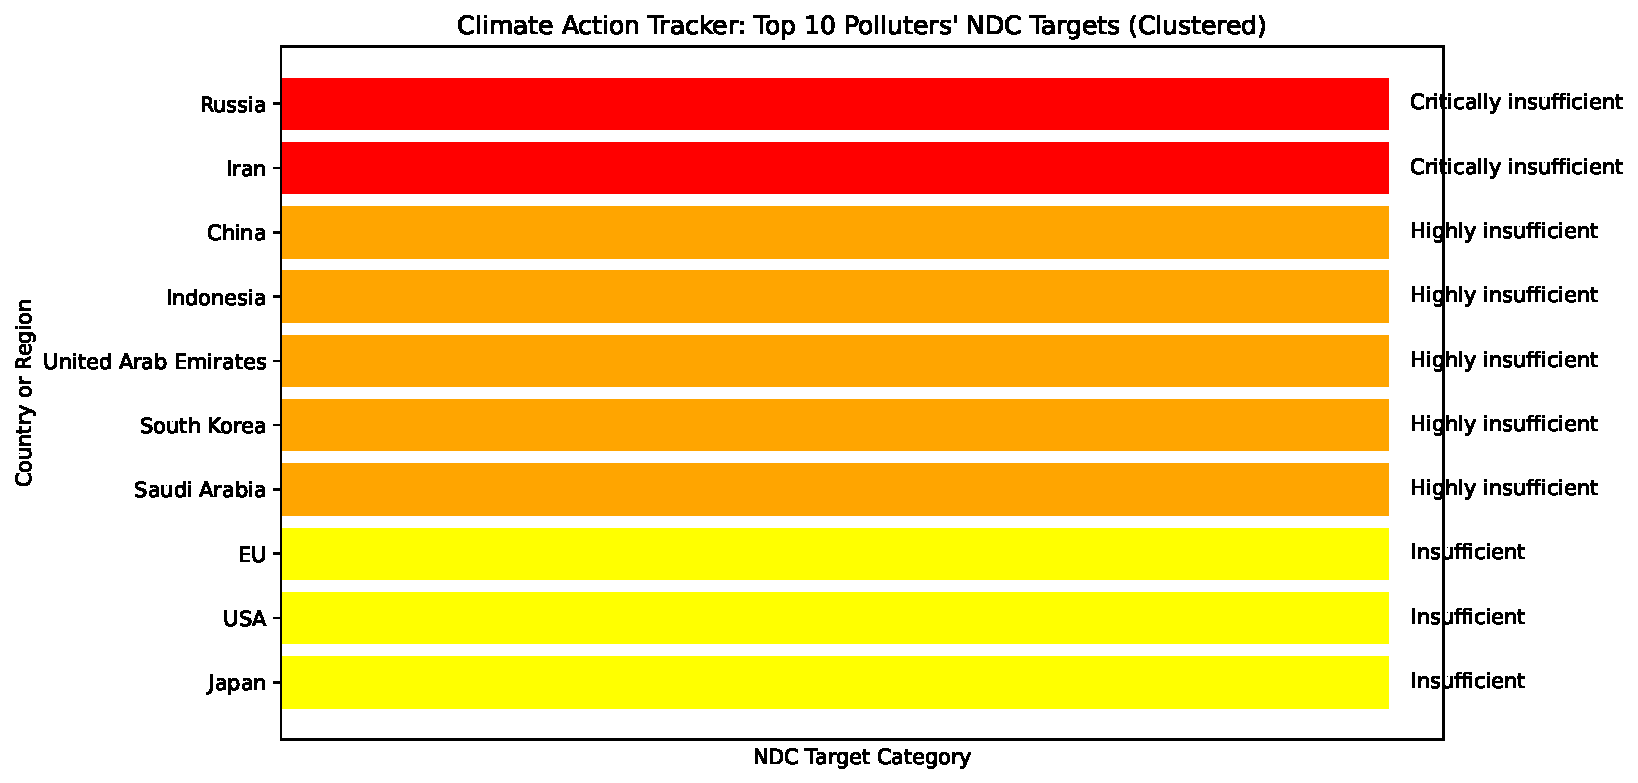
\includegraphics[keepaspectratio]{_thesis-nocite_files/figure-pdf/fig-ndcs-output-1.pdf}}

}

\caption[Nationally Determined Contributions
(NDCs)]{\label{fig-ndcs}Nationally Determined Contributions (NDCs)}

\end{figure}%

Fossil fuels are what powers humanity as well as the largest source of
CO\textsubscript{2} emissions. (IEA, 2022) reports ``Global
CO\textsubscript{2} emissions from energy combustion and industrial
processes rebounded in 2021 to reach their highest ever annual level. A
6\% increase from 2020 pushed emissions to 36.3 gigatonnes''. As on June
2023, fossil fuel based energy makes up 82\% of energy and is still
growing (Institute, 2023). The 425 largest fossil fuel projects
represent a total of over 1 gigaton in CO\textsubscript{2} emissions,
40\% of which were new projects Kühne et al. (2022). Tilsted et al.
(2023) expects the fossil fuel industry to continue to grow even faster.
In July 2023, the U.K. granted hundreds of new oil and gas of project
licenses in the North Sea (\emph{Rishi {Sunak} to Green-Light Hundreds
of New Oil and Gas Licenses in {North Sea}}, 2023).

(Ember, 2025) Ember's Electricity Data Explorer shows Taiwanese energy
usage based on data from Taiwanese government, visualizing the growth in
gas, wind, and solar, and decline of coal and nuclear power; however,
while declining, coal remains the leading power source for Taiwan.
Climate pledges made by international companies present in Taiwan mean
they need large amounts of green energy to meet their sustainability
goals. For instance, Google worked with the government of Taiwan to
change the laws to allow direct power procurement by foreign companies;
the current plan being to install 1 gigawatt of solar power fully
pre-purchased by the newly formed company created by BlackRock and
Google for boosting AI development as reported by (S. Chiang, 2024;
Jessop et al., 2024; 永鑫能源 New Green Power, 2022). More recently,
Google also purchased 10MW of geothermal energy for its Taiwanese AI
chip projects, doubling current Taiwanese geothermal capacity
(Hagström-Ilievska, Apr. 17, 2025 18:00; Potter, 2025; Jeffery Wu \&
Thompson, 2025). Geothermal energy provides 24/7 clean energy from the
Earth's core, however is limited due to lack of access; Taiwan happens
to be in geologically active spot on the ring of fire, where drilling
for geothermal energy is more feasible (M. Chang \& Hsiao, 2025; L,
2025b).

\subsubsection{Carbon Accounting, Emissions Trading
Schemes}\label{carbon-accounting-emissions-trading-schemes}

Trading CO\textsubscript{2e} emissions can be divided into 2 categories,
namely \emph{Compliance Carbon Markets} (CCM) and \emph{Voluntary Carbon
Markets} (VCM). The legislative baseline for Compliance Carbon Markets
is so low, people want to retire more CO\textsubscript{2e}, which they
can do through \emph{Voluntary Carbon Markets.}

As of 2024 there's no single global CO\textsubscript{2} trading market
but rather several local markets as described in the table below. Most
of the world is not part of a CO\textsubscript{2} market.

\def\pandoctableshortcapt{CO\textsubscript{2} Credit Trading Markets}

\begin{longtable}[]{@{}
  >{\raggedright\arraybackslash}p{(\linewidth - 4\tabcolsep) * \real{0.2639}}
  >{\raggedright\arraybackslash}p{(\linewidth - 4\tabcolsep) * \real{0.2639}}
  >{\raggedright\arraybackslash}p{(\linewidth - 4\tabcolsep) * \real{0.4722}}@{}}
\caption[CO~2~ Credit Trading Markets]{CO\textsubscript{2} credit
trading markets around the world from (\emph{International Carbon
Market}, n.d.).}\tabularnewline
\toprule\noalign{}
\endfirsthead
\endhead
\bottomrule\noalign{}
\endlastfoot
CO\textsubscript{2} Market & Launch Date & Comments \\
EU & 2005 & EU: (Araújo et al., 2020) \\
South Korea & 2015 & \\
China & 2021 & China's national emissions trading scheme (ETS) started
in 2021 priced at 48 yuan per tonne of CO\textsubscript{2}, averaged at
58 yuan in 2022 (Ivy Yin, 2023; H. Liu, 2021). \\
U.S. & 2013 & No country-wide market; local CO\textsubscript{2} markets
in California, Connecticut, Delaware, Maine, Maryland, Massachusetts,
New Hampshire, New York, Rhode Island, and Vermont \\
New Zealand & 2008 & New Zealand (Rontard \& Reyes Hernández, 2022)
(need access, important NCKU doesn't subscribe) \\
Canada & 2013 & \\
\end{longtable}

\let\pandoctableshortcapt\relax

The price of CO\textsubscript{2e} differs across markets, as assigning a
monetary value to reducing CO\textsubscript{2e} emissions depends on
several variables. (Stern, 2022b) argues carbon-neutral economy needs
higher CO\textsubscript{2e} prices and believes (Rennert et al., 2022)
CO\textsubscript{2e} price per ton should be 3,6x higher that it is
currently. Contrary, (Ritz, 2022) argues optimal CO\textsubscript{2}
prices could be highly asymmetric, low in some countries and high (above
the social cost of CO\textsubscript{2e}) in countries where production
is very polluting. The total size of carbon markets reached 949 billion
USD in 2023, including Chinese, European, and North American
CO\textsubscript{2} trading (LSEG \& Susanna Twidale, 02/12/2024, 02:37
PM).

The prices between compliance and voluntary markets differ
substantially.

\def\pandoctableshortcapt{Compliance Market CO\textsubscript{2} Prices}

\begin{longtable}[]{@{}ll@{}}
\caption[Compliance Market CO~2~ Prices]{Compliance market
CO\textsubscript{2} prices on August 12, 2023; data from (CarbonCredits,
2023; Ember, 2023; Trading Economics, 2023).}\tabularnewline
\toprule\noalign{}
\endfirsthead
\endhead
\bottomrule\noalign{}
\endlastfoot
Compliance Carbon Markets & Price (Tonne of CO\textsubscript{2}) \\
EU & 83 EUR \\
UK & 40 Pounds \\
US (California) & 29 USD \\
Australia & 32 USD \\
New Zealand & 50 USD \\
South Korea & 5.84 USD \\
China & 8.29 USD \\
\end{longtable}

\let\pandoctableshortcapt\relax

\def\pandoctableshortcapt{Voluntary Market CO\textsubscript{2} Prices}

\begin{longtable}[]{@{}ll@{}}
\caption[Voluntary Market CO~2~ Prices]{Voluntary market
CO\textsubscript{2} prices on August 12, 2023; data from (CarbonCredits,
2023).}\tabularnewline
\toprule\noalign{}
\endfirsthead
\endhead
\bottomrule\noalign{}
\endlastfoot
Voluntary Carbon Markets & Price (Tonne of CO\textsubscript{2}) \\
Aviation Industry Offset & \$0.93 \\
Nature Based Offset & \$1.80 \\
Tech Based Offset & \$0.77 \\
\end{longtable}

\let\pandoctableshortcapt\relax

\begin{figure}

\centering{

\pandocbounded{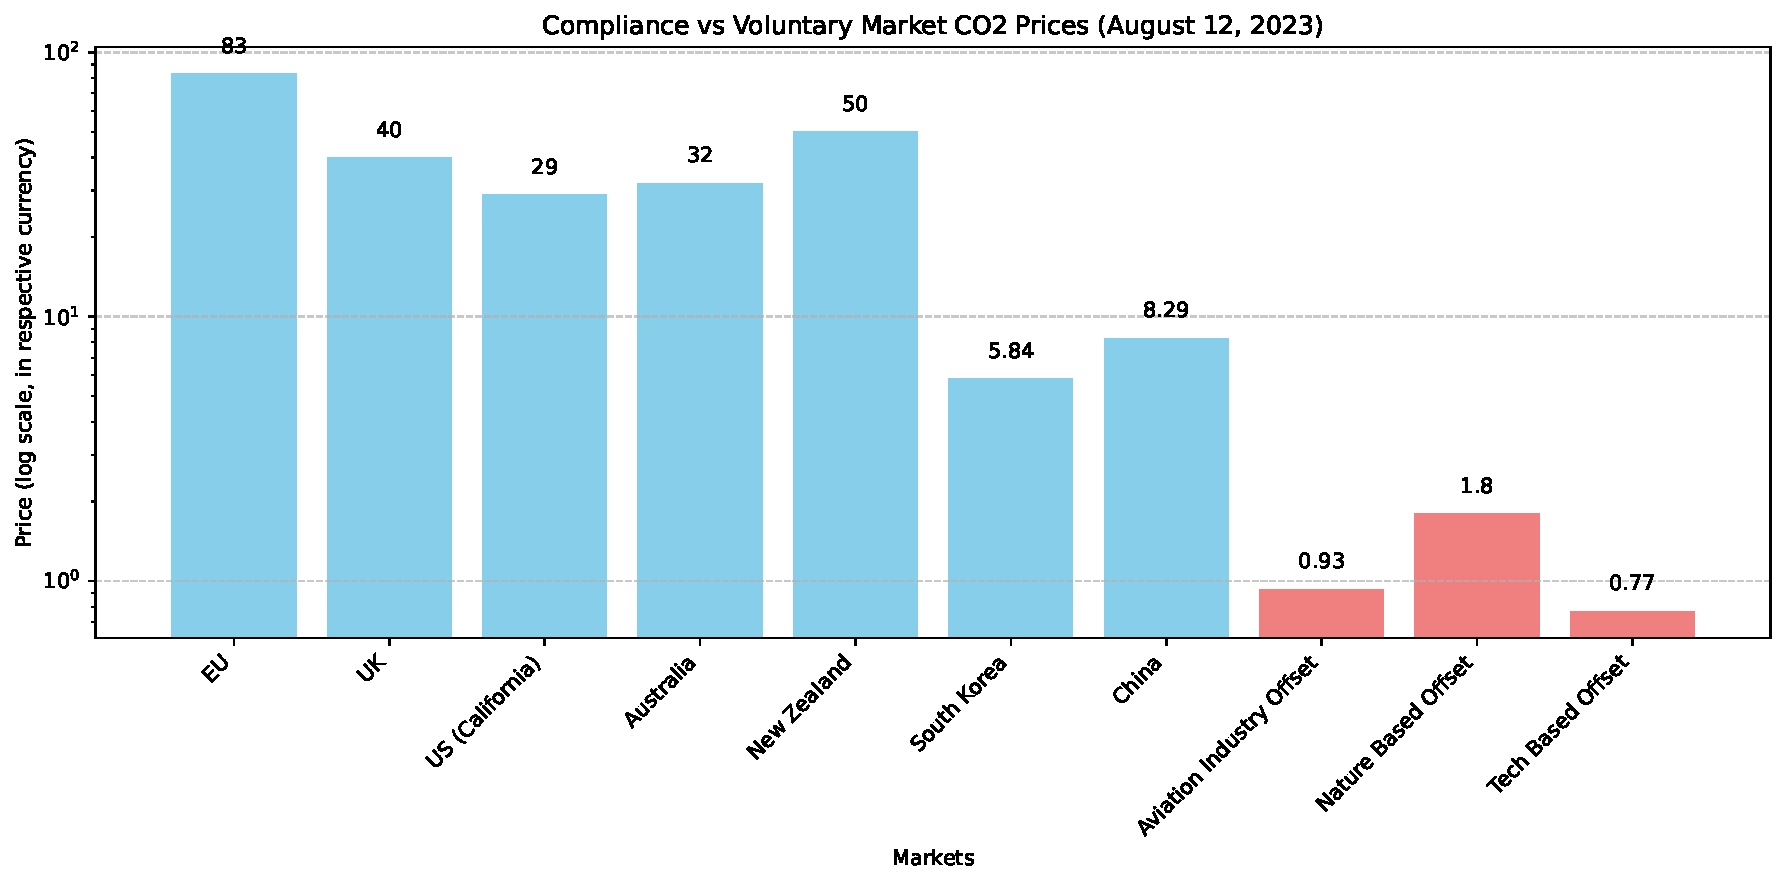
\includegraphics[keepaspectratio]{_thesis-nocite_files/figure-pdf/fig-carbon-cred-output-1.pdf}}

}

\caption[Carbon Credits]{\label{fig-carbon-cred}Carbon Credits}

\end{figure}%

Voluntary Carbon Markets are a decentralized system where private
entities voluntarily buy and sell carbon credits (ICVCM, 2025). Carbon
credits are useful for private companies who wish to claim \emph{carbon
neutrality, climate positivity}, or other related claim, which might be
viewed in good light by their clients or allow the companies to adhere
to certain legislative requirements. In the simplest terms, a carbon
credit represents 1T of CO\textsubscript{2}eq that has been prevented
from entering the atmosphere - or has been removed from circulation (aka
Carbon Credit Retirement) (Anna Watson, 2022, 2023). However it's
important to look at the details of these deal as Voluntary Carbon
Markets (VCM) lack standardization and transparency (Ela Khodai, 2023).
For example, Flickr only invested around 3000 USD in carbon credits and
got a carbon-neutral rating, which hardly seems enough for an
organization of its size (Climate Neutral, 2024).

Markets are centered around carbon credits, nature-backed financial
derivatives dependent on science-based methodologies for measurement,
reporting, and verification (MRV), which are managed and regularly
updated by certification organizations such as Gold Standard, Verra, and
others. Some standards released in the past few years include the Verra
Agricultural Land Management methodology for Verified Carbon Standard
(VCS) (Verra, 2023). Gold Standard recently released a methodology for
Mangrove-based carbon credits (Gold Standard, 2024). Regen Network
released a methodology for regenerative grazing systems, proposing
remote-sensing analysis with field-sampled soil carbon data, quantifying
GHG sequestration and ecological co-benefits (biodiversity,
water-infiltration, etc.) for robust MRV and carbon-credit issuance
(\emph{Methodology for {GHG} \& {Co-Benefits} in {Grazing Systems}},
2022). KlimaDAO, unhappy with the current standards, published ``An open
call for alternative carbon standards'' inviting carbon-credit issuers
and communities to propose next-generation registry frameworks and
leverage blockchain for transparency, liquidity and interoperability in
the voluntary carbon market (KlimaDAO, 2023a).

\def\pandoctableshortcapt{Criteria for Carbon Credit Projects}

\begin{longtable}[]{@{}
  >{\raggedright\arraybackslash}p{(\linewidth - 2\tabcolsep) * \real{0.5000}}
  >{\raggedright\arraybackslash}p{(\linewidth - 2\tabcolsep) * \real{0.5000}}@{}}
\caption[Criteria for Carbon Credit Projects]{Criteria for carbon credit
projects from (Verra, 2023).}\tabularnewline
\toprule\noalign{}
\begin{minipage}[b]{\linewidth}\raggedright
Criteria
\end{minipage} & \begin{minipage}[b]{\linewidth}\raggedright
Description
\end{minipage} \\
\midrule\noalign{}
\endfirsthead
\toprule\noalign{}
\begin{minipage}[b]{\linewidth}\raggedright
Criteria
\end{minipage} & \begin{minipage}[b]{\linewidth}\raggedright
Description
\end{minipage} \\
\midrule\noalign{}
\endhead
\bottomrule\noalign{}
\endlastfoot
Baseline & Ecosystem carbon sequestration rate without the intervention
(project) \\
Additionality & New carbon capture or prevention of emissions \\
Permanence & Carbon storage time (should be long-term) \\
Leakage & Risk of shift to causing emissions (for example because of
deforestation) \\
\end{longtable}

\let\pandoctableshortcapt\relax

For the individual person, there's no direct access to
CO\textsubscript{2} markets. However, brokers do buy large amounts of
carbon credits to resell in smaller quantities to retail investors.
Facilitating citizens' access to CO\textsubscript{2} emissions trading
may be an efficient method to organize large-scale CO\textsubscript{2}
retiring (Rousse, 2008). (Sipthorpe et al., 2022) compares traditional
and blockchain-based solutions to carbon trading, arguing that
blockchain solutions for CO\textsubscript{2}eq markets are nearing
maturity, and offer many improvements, such as enhancing transparency,
trust, and efficiency.

CO\textsubscript{2e} credits have given rise to the Carbon Accounting
industry, to help companies meet legal emissions reduction targets in
Compliance Carbon Markets, with many companies like Watershed, Greenly,
and Sustaxo providing services. (Quatrini, 2021) admits sustainability
assessments are often complex and may give flawed results. Nonetheless,
CO\textsubscript{2} emission reduction has the added positive effect of
boosting corporate morale (J. Cao et al., 2023).

There are many companies which facilitate buy carbon credits as well as
a few organizations focused on carbon credit verification. In Estonia,
startups Arbonics and Single.Earth are trialing this approach in several
forests. The most established certifiers or carbon credits include the
Verified Carbon Standard (VCS), the Gold Standard, Climate Action
Reserve (CAR)‍, and the American Carbon Registry (ACR).

\emph{``Carbon pricing is not there to punish people,''} says Lion Hirth
(Lion Hirth, n.d.). \emph{``It's there to remind us, when we take
travel, heating, consumption decisions that the true cost of fossil
fuels comprises not only mining and processing, but also the damage done
by the CO\textsubscript{2} they release.''} Long term cost of
insufficient climate action is more than short-term gains from delaying
efforts to reduce carbon emissions. In addition to the damages from
global warming, the fossil energy production that's a large part of
global CO\textsubscript{2}eq emissions has caused several high-profile
pollution events. Large ones that got international news coverage
include Exxon Valdez and Deepwater Horizon.

Carbon credit prices should reflect the quality of the carbon reduction.
Nature-based carbon removal solutions (for example, forest-backed carbon
credits) rank among the top solutions for mitigating climate change but
require price signals that reflect their true value; Pachama's (an
AI-based carbon removal company) calculation from bottom up cost
modeling across more than 150 reforestation projects indicate that high
quality forest carbon removal credits must trade at a minimum of USD
50-82 per tonne of CO\textsubscript{2}eq to be competitive with
alternative land uses (IPCC AR6 guidance sets the price spread wider,
from USD 50-200); reduced land-use change (basically this means not
cutting down forests, IPCC groups together as LULUCF, Land Use, Land-Use
Change and Forestry) ranks 2nd to solar energy in terms of carbon
reduction potential (Luik, 2025; Pachama, 2023).

\subsubsection{Markets Financialize the Natural World: Pricing, Tracing,
and Trading Ecosystem Services and Nature-backed
Assets}\label{markets-financialize-the-natural-world-pricing-tracing-and-trading-ecosystem-services-and-nature-backed-assets}

Similarly to carbon markets, markets for nature-backed assets and
ecosystem services are centered around different types of credits.

\def\pandoctableshortcapt{Types of Nature-Backed Assets and Tradeable
Ecosystem Services}

\begin{longtable}[]{@{}
  >{\raggedright\arraybackslash}p{(\linewidth - 2\tabcolsep) * \real{0.3194}}
  >{\raggedright\arraybackslash}p{(\linewidth - 2\tabcolsep) * \real{0.6806}}@{}}
\caption[Types of Nature-Backed Assets and Tradeable Ecosystem
Services]{Types of nature-backed assets and tradeable ecosystem services
(Borges et al., 2022; Deloitte, 2024; Fiegenbaum, 2024; PWC, 2025;
Rossberg et al., 2024; U.S. Securities and Exchange Commission,
2023)}\tabularnewline
\toprule\noalign{}
\begin{minipage}[b]{\linewidth}\raggedright
\textbf{Asset Type}
\end{minipage} & \begin{minipage}[b]{\linewidth}\raggedright
\textbf{Description}
\end{minipage} \\
\midrule\noalign{}
\endfirsthead
\toprule\noalign{}
\begin{minipage}[b]{\linewidth}\raggedright
\textbf{Asset Type}
\end{minipage} & \begin{minipage}[b]{\linewidth}\raggedright
\textbf{Description}
\end{minipage} \\
\midrule\noalign{}
\endhead
\bottomrule\noalign{}
\endlastfoot
Carbon Credits and Offsets & Represent avoided or removed
CO\textsubscript{2}eq emissions through reforestation, soil health
improvements, regenerative farming practices that sequester carbon,
etc \\
Biodiversity Credits & Represent conservation and restoration of species
or ecosystems quantified by some standard or criteria such as provided
by Verra and Gold Standard \\
Water Rights and Wetland Credits & Represent rights to access water or
preserve/restore wetlands which can be traded \\
Conservation Finance Instruments & Represent bonds or funds that protect
forests, coral reefs, or species habitats \\
Natural Asset Companies (NACs) & Represents a SEC-backed structure
allowing public trading of ecosystem ownership rights \\
Tokenized Natural Resources & Represent blockchain-based representations
of nature (e.g., tokenized forest) \\
\end{longtable}

\let\pandoctableshortcapt\relax

\subsubsection{Overconsumption \textgreater{} Earth's
Boundaries}\label{overconsumption-earths-boundaries}

Excessive consumer lifestyle - \emph{overconsumption} - is one of the
main drivers of climate change and environmental destruction, with
\emph{``2/3 of global GHG emissions are directly and indirectly linked
to household consumption, with a global average of about 6 tonnes
CO\textsubscript{2} equivalent per capita''} , according to (Ivanova et
al., 2020; Renee Cho, 2020). An older study put the number as high as
60\% percent (Ivanova et al., 2016) while (Ellen MacArthur Foundation,
Material Economics, 2019)'s models 45\% show of CO\textsubscript{2}
equivalent emissions come from our shopping; produced by companies to
make the products we consume. (Keeble, 1988) reported in April 1987 that
\emph{`residents in high-income countries lead lifestyles incompatible
with planetary boundaries'}. (Ivanova et al., 2020) reports the average
footprint in North America and Europe is 13.4 t CO\textsubscript{2}eq,
in Africa and the Middle East 1.7t CO\textsubscript{2}eq; consumption
options with a high mitigation potential measured in tonnes of
CO\textsubscript{2} equivalent per capita per year include
\emph{``living car-free''} and avoiding flying, which could each save
upwards of 1.7t CO\textsubscript{2}eq per person annually.

While the numbers on overconsumption are clear, the debate on
overconsumption is so polarized, it's difficult to have a meaningful
discussion of the topic (Ianole \& Cornescu, 2013). Environmental risks
from human activities are known as Anthropogenic Threat Complexes (ATCs)
(Bowler et al., 2020). With the trend of urbanization, it's not
surprising (people living in) cities are responsible for 80\% of the
emissions (Rosales Carreón \& Worrell, 2018). (Moberg et al., 2019)
reports daily human activities emission contribution on average in four
European countries (France, Germany, Norway and Sweden).

\def\pandoctableshortcapt{Daily Human Activities' Emission Contribution}

\begin{longtable}[]{@{}ll@{}}
\caption[Daily Human Activities' Emission Contribution]{Daily human
activities emission contribution, on average, in France, Germany, Norway
and Sweden from (Moberg et al., 2019).}\tabularnewline
\toprule\noalign{}
\endfirsthead
\endhead
\bottomrule\noalign{}
\endlastfoot
Emission Share & Category \\
21\% & Housing \\
30\% & Food \\
34\% & Mobility \\
15\% & Other \\
\end{longtable}

\let\pandoctableshortcapt\relax

Taking a broader view, (Hannah Ritchie, 2020; US EPA, 2016) dissect GHG
emissions inventory by sector and put the blame squarely on the type of
energy used.

\def\pandoctableshortcapt{Industrial Emissions}

\begin{longtable}[]{@{}
  >{\raggedright\arraybackslash}p{(\linewidth - 4\tabcolsep) * \real{0.2222}}
  >{\raggedleft\arraybackslash}p{(\linewidth - 4\tabcolsep) * \real{0.2222}}
  >{\raggedright\arraybackslash}p{(\linewidth - 4\tabcolsep) * \real{0.5556}}@{}}
\caption[Industrial Emissions]{Industrial Emissions (Hannah Ritchie,
2020; US EPA, 2016).}\tabularnewline
\toprule\noalign{}
\begin{minipage}[b]{\linewidth}\raggedright
Sector
\end{minipage} & \begin{minipage}[b]{\linewidth}\raggedleft
Share
\end{minipage} & \begin{minipage}[b]{\linewidth}\raggedright
Description
\end{minipage} \\
\midrule\noalign{}
\endfirsthead
\toprule\noalign{}
\begin{minipage}[b]{\linewidth}\raggedright
Sector
\end{minipage} & \begin{minipage}[b]{\linewidth}\raggedleft
Share
\end{minipage} & \begin{minipage}[b]{\linewidth}\raggedright
Description
\end{minipage} \\
\midrule\noalign{}
\endhead
\bottomrule\noalign{}
\endlastfoot
Energy Use (inc. electricity, heat and transport) & 73.2 \% & Total
CO\textsubscript{2}eq emissions from all fuel combustion and related
fugitive losses. Energy use in industry (24.2\%) in processing metals
(iron and steel), chemicals and petrochemicals, food and tobacco, non
ferrous metals, paper, machinery, other industry; transport (16.2\%)
road, aviation, shipping, rail; buildings (17.5\%) including residential
and commercial; fugitive emissions (5.8\%) such as methane leaks from
oil and gas exploitation and coal mining; plus other, unallocated fuel
combustion related emissions (7.8\%) \\
Direct Industrial Processes & 5.2 \% & Direct CO\textsubscript{2}eq
emissions from chemical reactions in cement and in chemicals and
petrochemicals. \\
Waste & 3.2 \% & Wastewater methane and NO2 emissions; landfill
methane. \\
Agriculture + LULUCF (Land Use, Land-Use Change \& Forestry) & 18.4 \% &
Emissions from grassland, cropland, deforestation, crop burning, rice
cultivation, agricultural soils, livestock and manure. \\
\end{longtable}

\let\pandoctableshortcapt\relax

Earth's growing population reached 8 Billion people In November 2022 and
population projections by predict 8.5B people by 2030 and 9.7B by 2050
(The Economic Times, 2022; United Nations Department of Economic and
Social Affairs, Population Division, 2022). Indeed, making
\emph{anything} consumes natural resources, which are limited on planet
Earth. (Hassoun et al., 2023) forecasts increase of global food demand
by 62\% driven by the impact of climate change. Yet, while population
growth puts higher pressure on Earth's resources, some researchers
propose the effect is higher from wasteful lifestyles than the raw
number of people (Cardinale et al., 2012). Meanwhile, others, such as
(Cafaro et al., 2022), believe \emph{{[}o{]}verpopulation is a major
cause of biodiversity loss and smaller human populations are necessary
to preserve what is left.''}

\subsubsection{Plastic Pollution}\label{plastic-pollution}

Overconsumption is also one of the root causes of plastic pollution.
(Ford et al., 2022) and (Lavers et al., 2022) find strong links between
climate change and marine plastic pollution \emph{``along with other
stressors that threaten the resilience of species and habitats sensitive
to both climate change and plastic pollution''}.

Plastic pollution is pervasive around the Earth and is fundamentally
linked to climate change, while microplastics are increasingly a real
concern (Lavers et al., 2022; Tiernan et al., 2022). Several
international studies report recent findings of microplastics everywhere
in human bodies: the brain, lungs, digestive tissues, bone marrow,
penis, testis, seminal fluid (semen), and placenta - causing serious
health and reproductive concerns (Codrington et al., 2024; M. A. Garcia
et al., 2024; Guo et al., 2024; Hu et al., 2024; N. Li et al., 2024;
Main, 2024; Montano et al., 2023; L. Zhu et al., 2024)

\begin{figure}

\centering{

\pandocbounded{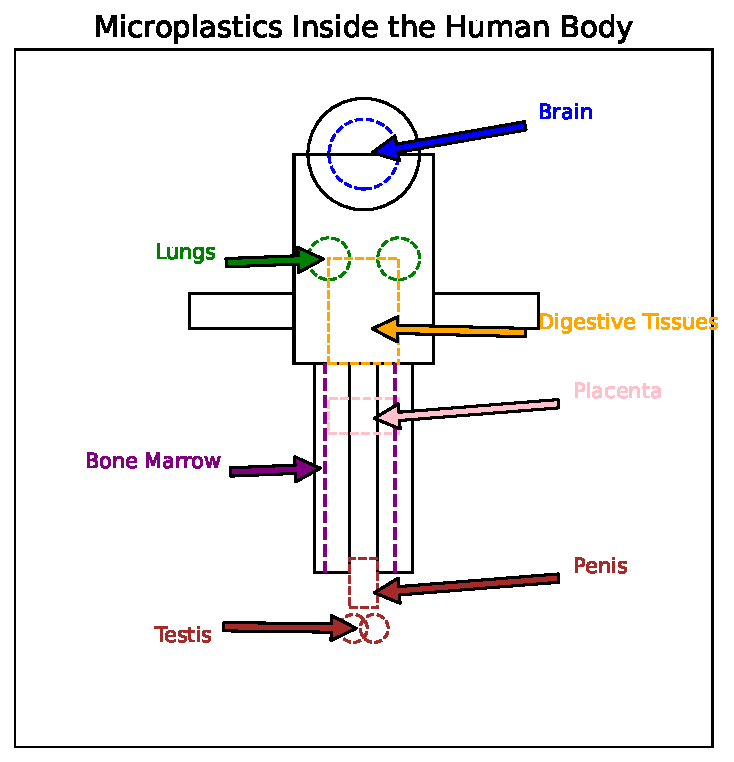
\includegraphics[keepaspectratio]{_thesis-nocite_files/figure-pdf/fig-microplastics-output-1.pdf}}

}

\caption[Microplastics in the Human
Body]{\label{fig-microplastics}Microplastics in the Human Body}

\end{figure}%

In addition to the enormity of over-reaching CO\textsubscript{2}
emissions, humanity is facing other massive environmental problems. The
Stockholm Resilience Centre report in 2022 we have already breached 4
out of our 9 \emph{``planetary boundaries'':} in addition to climate
change, biodiversity loss (Extinctions per Million Species per Year aka
E/MSY), land-system change (deforestation, land degradation, etc), and
biogeochemical flows (cycles of carbon, nitrogen, phosphorus, etc); on a
positive side, the challenges of fresh water use, ocean acidification
and stratospheric ozone depletion are still within planetary limits
(Persson et al., 2022).

An update to the planetary boundaries framework a year later found the
actual number to be 6 of 9 boundaries (climate, biosphere integrity,
land use, biogeochemical flows, freshwater use, novel entities) already
transgressed, with ocean acidification nearing its limit and only
stratospheric ozone recovering; atmospheric aerosol loading and the
biodiversity intactness index (BII), which belongs under biodiversity
loss and measures how depleted are the species that are still around
(but not yet extinct), were quantified recently (Newbold et al., 2016;
Richardson et al., 2023).

In the biosphere, mass extinctions are underway. An analysis of
population trends for 27600 terrestrial vertebrate species (including a
detailed sample of 177 mammals), found 32\% (8851 species) are
undergoing severe range contractions; the authors name this ``biological
annihilation'' to signal Earth's ongoing 6 mass extinction and call for
immediate conservation action (Ceballos et al., 2017). As of last year,
the Red List curated by the International Union for Conservation of
Nature (IUCN), includes 45,300 species (28\% of all assessed, since IUCN
was founded in 1948), under threat of extinction (IUCN, 2024).

Responding to the crisis, the Guardian newspaper in the UK has taken a
clear stance, covering stories of extinction; the \emph{Area de
Conservación Guanacaste} is one of the protected areas listed by the
UNESCO World Heritage Centre, providing data on the State of
Conservation (SOC) by year (Centre, 1999; McClure, 2025)

\begin{figure}

{\centering 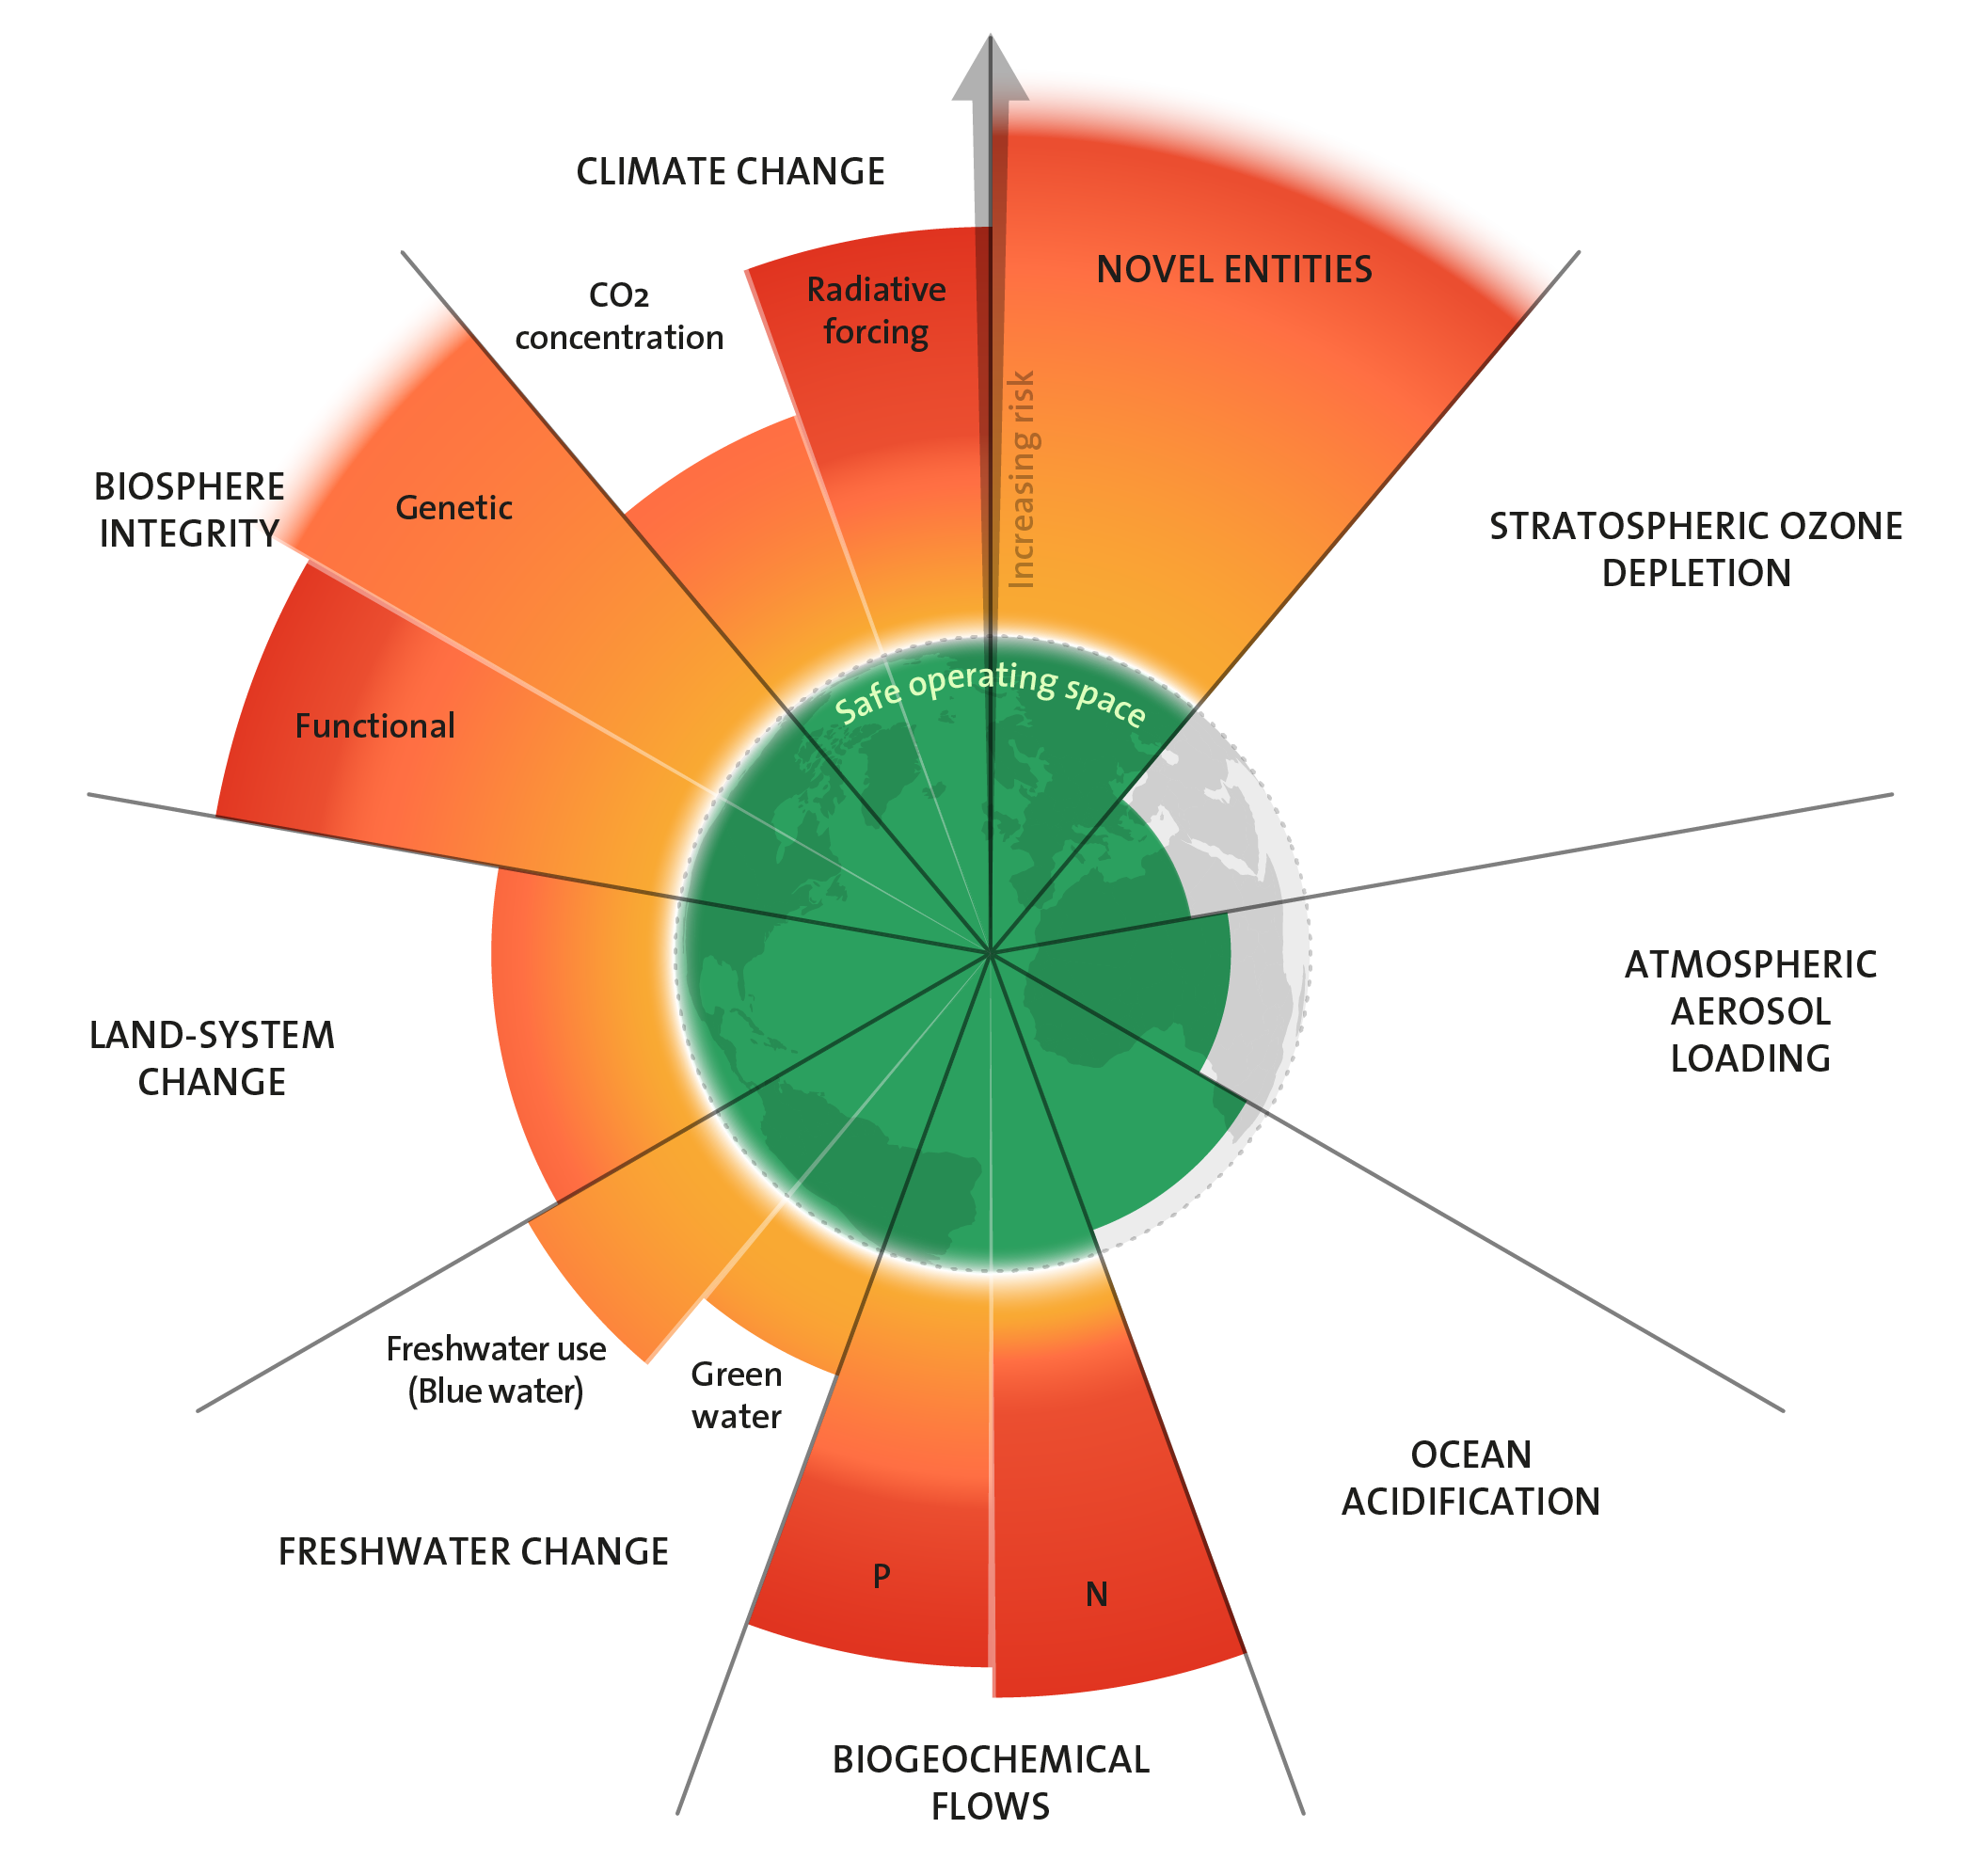
\includegraphics[width=1\linewidth,height=\textheight,keepaspectratio]{./images/sustainability/planetary-boundaries-2023.png}

}

\caption[Planetary Boundaries 2023 Update]{Planetary Boundaries 2023
update. Azote for Stockholm Resilience Centre, based on analysis in
Richardson et al 2023}

\end{figure}%

In 2018 Swedish Sportswear brand Houdini launched the first corporate
planetary boundaries' assessment in partnership with Albaeco and
Stockholm Resilience Centre to establish a baseline for its ``impact
positive'' ambition (Houdini, 2018). While it's a pilot study, it
demonstrates how companies can integrate system-level science into
sustainability reporting (Haeggman et al., 2018). At the 2024 update for
the report, Houdini invited, Johan Rockström, a renown conservation and
climate scientist, envisions a global dashboard of the development of
the economy and the state of the planetary boundaries, with high
resolution maps, to help visualize Earth's situation in real-time
(Houdini Sportswear, 2024).

\subsubsection{Evolving Measurements from Planetary Health to Earth
System Law, and Social Cost of
Carbon}\label{evolving-measurements-from-planetary-health-to-earth-system-law-and-social-cost-of-carbon}

Scientists in cross-disciplinary teams have been working on integrating
Earth systems and human society into cohesive frameworks. (Wardani et
al., 2023) stresses that every facet of Earth's life-support
system---living biota and the ``abiotic'' foundations of climate, water,
soils, and geology---co-produces the conditions for civilization:
\emph{``long-term human well-being is dependent on the well-being of the
planet, including both biotic and abiotic systems. It recognizes
interlinkages across environmental sustainability, public health, and
socioeconomic development.''}

There are 3 approaches that address the complex interdependence of
humans with our physical environment, that have the potential to be
complementary - \emph{Planetary Health}, \emph{Social Cost of Carbon},
and \emph{Earth System Law}.

\emph{Planetary Health} is a framework rooted in public health sciences
and medicine; what if public health leveled-up to planetary scale,
concerned with the health of ecological life-support systems: clean air,
food, and a safe climate, so they can support human flourishing; in
practice the framework focuses on evidence, education, governance, and
business (Planetary Health Alliance, 2024a, 2024b).

\emph{Social Cost of Carbon} attempts to measure the compound impact of
CO\textsubscript{2e} emissions on society. Sustainability is filled with
complexities. CO\textsubscript{2e} emissions are complicated by
biodiversity loss, child labor, slavery, poverty, chemical pollution,
etc. - many issues become intertwined (TEDx Talks, 2020). One attempt to
measure these complexities, is the \emph{Social Cost of Carbon} (SCC)
which is defined as \emph{``additional damage caused by an extra unit of
emissions''} (Kornek et al., 2021; Zhen et al., 2018). For example the
cost of damages caused by ``one extra ton of carbon dioxide emissions''
(Stanford University, 2021). SCC variations exist between countries
(Tol, 2019) and regions (Yong Wang et al., 2022).

\emph{Earth System Law} is a framework rooted in the legal sciences for
addressing interconnected environmental challenges in a hyper-connected
Earth, where climate feedbacks, and environmental thresholds don't
respect country borders; in practice, this line of thinking helps to
develop carbon-budget clauses inside trade deals and biodiversity
``safety brakes'' that trigger when monitoring data shows an Earth
boundary overshoot, potentially acting as the legal scaffolding that
lets Planetary Health prescriptions and Social Cost of Carbon price
signals be effective (Du Toit \& Kotzé, 2022).

More recently, because of the complex interdependence, (J. Zhang et al.,
2025) proposes a new sustainability index that systematically considers
pertinent indicators of interdependencies and interactions across
different dimensions of sustainability. Moreover, (Lenton et al., 2023)
proposed a new innovative way to quantify the ``cost'' of global warming
in human terms by counting the number of people forced outside the
``human climate niche'' (temperatures historically occupied by most
humanity); climate change has already exposed ≈9\% of today's population
(\textgreater600 million) unprecedented heat stress, risking increased
mortality, morbidity and displacement; if current trends continue by
2100, \textasciitilde2.7 °C, 21--39 \% or 2--4 billion people will be
exposed by 2080--2100.

\subsection{Quantifying Human Benefits from the Biosphere: Ecosystem
Services}\label{quantifying-human-benefits-from-the-biosphere-ecosystem-services}

\emph{Ecosystem services measure the benefits humans receive from the
biosphere.} Put simply, \emph{ecosystem services} enable human life on
Earth - we are, in a very real sense, - dependent on nature. The
biosphere is Earth's life support system. Earth's biosphere is made up
of 846 terrestrial ecoregions, which are distributed across 14 major
biomes and 8 biogeographical realms (Dinerstein et al., 2017).

While it can be assumed much of the flora and fauna are crucial for
Earth's systems, science is still in the process of understanding and
quantifying its contributions. The history of the valuation of nature's
services goes back to the 18th century when David Ricardo and Jean
Baptiste Say discussed nature's \emph{work}, however both considered it
should be free (Gómez-Baggethun et al., 2010). In 1997 (Daily, 1997)
proposed the idea of \emph{ecosystem services} and (Costanza et al.,
1997) attempted to assess the amount of ecosystem services provided. (Le
Provost et al., 2022)'s study shows \emph{biodiversity} as one key
factor to maintain delivery of ecosystem services. (Noriega et al.,
2018) attempts to quantify the ecosystem services (ES) provided by
insects.

The most complex computer models which attempt to capture ever more
interactions happening in the physical realm are called \emph{digital
twins.} The EU is developing a digital twin of Earth to help
sustainability prediction and planning, integrating Earth's various
systems such as climate, hydrology, ecology, etc., into a single model
(\emph{Destination {Earth} {\textbar} {Shaping Europe}'s Digital
Future}, 2023; J. Hoffmann et al., 2023). For instance, AI is being used
to map icebergs and measure the change in size (European Space Agency,
2023). We can use all the data being recorded to provide a digital twin
of the planet, nature, ecosystems and human actions to help us change
our behavior and optimize for planetary wellbeing.

\subsubsection{Ecological Indicators to Track Environmental
Health}\label{ecological-indicators-to-track-environmental-health}

\subsubsection{Measuring Biodiversity Loss, Ecological Indicators and
Environmental
Degradation}\label{measuring-biodiversity-loss-ecological-indicators-and-environmental-degradation}

Sustainability can be measured using a variety of \emph{ecological
indicators}. Ecological indicators for Earth \emph{- I would like to
coin the word ``ecomarkers'' -} are like \emph{biomarkers} in human
health. Technological advances help scientist better understand nature.
Cutting edge research uses AI-based voice recognition for listening to
nature, assessing biodiversity based on species' sounds in the forest.
Millions of detections of different species with machine learning
passive acoustic AI models, can also assess species' response to climate
change (AI for Good, 2023; Guerrero et al., 2023).

Around the world, pressure on ecosystems is rapidly increasing, with
biodiversity destruction ever prevalent, making protecting biodiversity
as urgent as protecting the climate. (Almond, R.E.A. et al., 2022)
reported, the number of species killed, mass destruction of nature:

\begin{quote}
\emph{``69\% decline in the relative abundance of monitored wildlife
populations around the world between 1970 and 2018. Latin America shows
the greatest regional decline in average population abundance (94\%),
while freshwater species populations have seen the greatest overall
global decline (83\%).''}
\end{quote}

In Europe, as of 2025, none of the evaluated biodiversity targets are on
track; agricultural targets, such as reducing soil nutrient losses, and
reducing fertilizer use, are particularly lagging (European Commission,
2025).

\emph{Environmental DNA (eDNA)} helps scientists measure species
abundance without direct observation through detection of DNA on genetic
materials such as skin cells (Peter Andrey Smitharchive page, 2024).
Cellular DNA can be isolated from various sediment types (Ogram et al.,
1987). Beyond scientific applications, eDNA is being used to generate
biodiversity credits by environmental asset rating companies such as
BeZero, a ratings' agency for the Voluntary Carbon Market (Ojoatre \&
Atkinson, 2023).

Similarly to climate protection, the UN has taken a leadership role in
biodiversity protection, by organizing an annual Convention on
Biodiversity. The history of the United Nations Convention on
Biodiversity goes back to 1988, when the working group was founded
(Unit, 2023). The Convention on Biodiversity 2022 (COP15) adopted the
first global biodiversity framework to accompany climate goals (UNEP,
Tue, 12/20/2022 - 07:44).

\def\pandoctableshortcapt{Biodiversity Loss}

\begin{longtable}[]{@{}
  >{\raggedright\arraybackslash}p{(\linewidth - 2\tabcolsep) * \real{0.6111}}
  >{\raggedright\arraybackslash}p{(\linewidth - 2\tabcolsep) * \real{0.3889}}@{}}
\caption[Biodiversity Loss]{Biodiversity loss data from (Bradshaw et
al., 2021).}\tabularnewline
\toprule\noalign{}
\endfirsthead
\endhead
\bottomrule\noalign{}
\endlastfoot
What Happened? & How Much? \\
Vertebrate species population average decline & 68\% over the last 50
years \\
Land surface altered by humans & 70\% of Earth \\
Vertebrate species extinct & 700 in 500 years \\
Plant species extinct & 600 in 500 years \\
Species under threat of extinction & 1 million \\
\end{longtable}

\let\pandoctableshortcapt\relax

\begin{figure}

\centering{

\pandocbounded{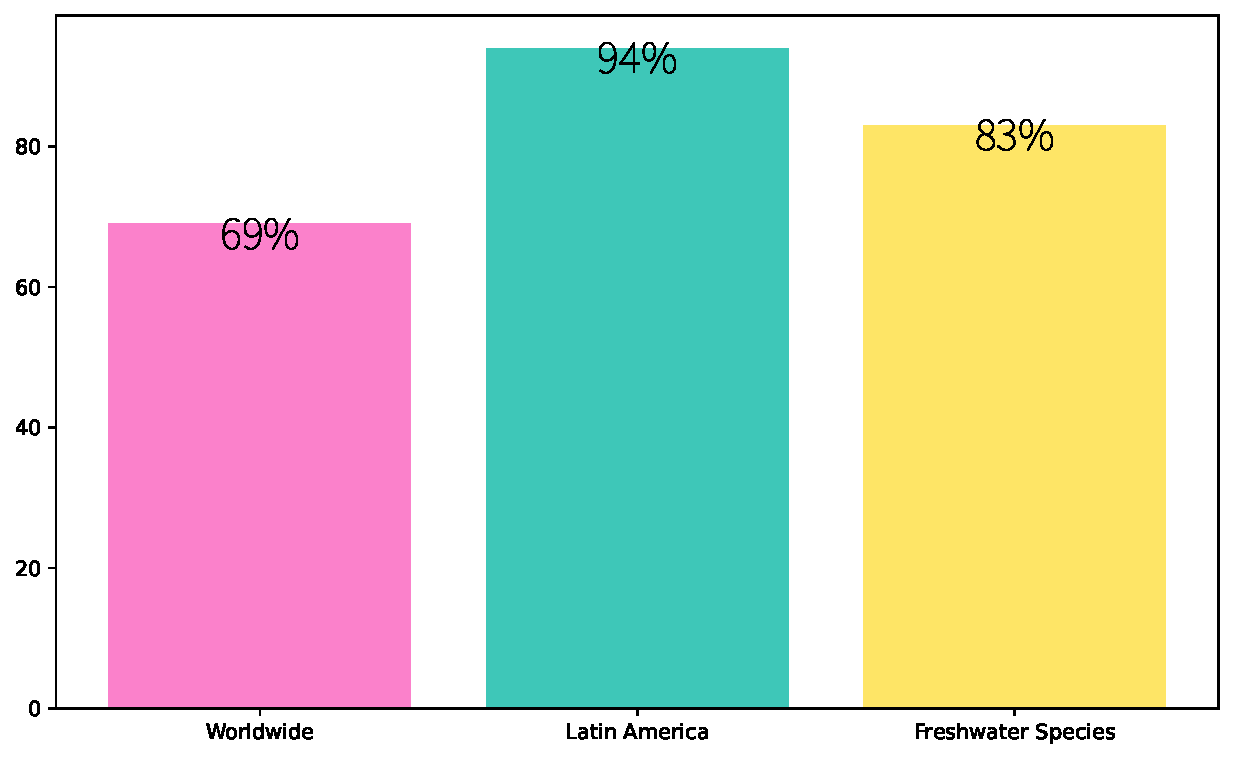
\includegraphics[keepaspectratio]{_thesis-nocite_files/figure-pdf/fig-biod-loss-output-1.pdf}}

}

\caption[Biodiversity Loss]{\label{fig-biod-loss}Biodiversity Loss}

\end{figure}%

Biodiversity loss is linked to overconsumption, weak legislation and
lack of oversight. (Crenna et al., 2019) recounts European Union
consumers' negative impact on biodiversity in countries where it imports
food. (WWF, 2022) case study highlights how 4 biodiverse regions Cerrado
in Brazil, Chaco in Argentina, Sumatra in Indonesia, and the Cuvette
Centrale in Democratic Republic of Congo are experiencing rapid
destruction due to consumer demand in the European Union. While the
European Union (EU) has recently become a leader in sustainability
legislation, biodiversity protection measures among private companies is
very low Marco-Fondevila \& Álvarez-Etxeberría (2023).

Starting with the simple question: why protect biodiversity. (May, 2011)
argues biodiversity loss is a concern for 3 points of views:

\def\pandoctableshortcapt{Ethical and Utilitarian Concepts of
Biodiversity Protection}

\begin{longtable}[]{@{}
  >{\raggedright\arraybackslash}p{(\linewidth - 2\tabcolsep) * \real{0.3611}}
  >{\raggedright\arraybackslash}p{(\linewidth - 2\tabcolsep) * \real{0.6389}}@{}}
\caption[Ethical and Utilitarian Concepts of Biodiversity
Protection]{Ethical and Utilitarian Concepts of Biodiversity Protection
from (May, 2011).}\tabularnewline
\toprule\noalign{}
\endfirsthead
\endhead
\bottomrule\noalign{}
\endlastfoot
Point of View & Description \\
Narrowly Utilitarian & Biodiversity is a resource of genetic novelties
for the biotech industry. \\
Broadly Utilitarian & Humans depend upon biodiverse ecosystems. \\
Ethical & Humans have a responsibility to future generations to pass
down a rich natural world. \\
\end{longtable}

\let\pandoctableshortcapt\relax

There is some progress in biodiversity conservation as
``{[}*b{]}iodiversity awareness is now at 72\% or higher in all
countries sampled, compared to only 29\% or higher across countries
sampled in 2009''* (UEBT, 2022)

\subsubsection{Oceans and Marine Ecosystem
Sustainability}\label{oceans-and-marine-ecosystem-sustainability}

Marine heatwaves are intensifying under climate change, threatening
species diversity and the ocean's capacity to supply critical services
from fisheries to carbon sequestration (Smale et al., 2019).
Accelerating ocean warming, evidenced by record-breaking sea-surface
temperatures, has triggered widespread coral bleaching, clearly visible
at the Great Barrier Reef in Queensland, East Coast of Australia, loss
of marine habitat complexity, and cascading threats to coastal economies
and food security; the authors call for integrated climate--ocean policy
action, stressing that without urgent emissions cuts and ecosystem-based
adaptation, the ocean's capacity to regulate climate and sustain
biodiversity will collapse (Gelles \& Andreoni, 2023; Pfeiffer, 2024).
Cumulative pressures: climate extremes, pollution, and overexploitation
- have driven evolutionary shifts in marine life and unpredictably
altered ecosystem-service delivery (Espinosa \& Bazairi, 2023).

Some earlier studies, such as (Howard et al., 2017) demonstrate how
integrating blue carbon habitats into Marine Protected Area (MPA) design
can both mitigate carbon emissions and enhance ecosystem resilience.
Meta-analyses across 121 sites in 87 MPAs globally show that most
well-designed and managed MPAs achieve significant ecological gains: on
average, fish biomass inside no-take zones can double to triple compared
with outside areas, and species richness likewise increases by 20--30 \%
within 5--10 years of enforcement (Rudd, 2015). However, Marine
Protected Areas cover only 8\% of the world's oceans and only 2.8\% is
effectively protected (Igini, 2024a). The UN's 30x30 target (set under
the Convention on Biological Diversity) aims to protect 30\% of the
world's oceans by 2030, however is not on track to achieve this goal
(Mouterde, 2024).

\subsubsection{Forests: Carbon Sinks and Biodiversity
Reservoirs}\label{forests-carbon-sinks-and-biodiversity-reservoirs}

Forests are a crucial part of Earth's carbon cycle and the main natural
CO\textsubscript{2} capture system; due to deforestation, Europe rapidly
losing its forest carbon sink (Frédéric Simon, 2022). Beyond their role
in locking away carbon, recent field work shows forest actively scrub
methane from the air as tree bark absorbs methane (Gauci et al., 2024).
Around 27\% of Earth's land area is still covered by forests, yet
\emph{deforestation} is widespread all around the world; highest rates
of deforestation happened in the tropical rainforests of South America
and Africa, mainly caused by agricultural cropland expansion (50\% of
all deforestation) and grazing land for farm animals to produce meat
(38.5\%), totaling close to 90\% of global deforestation (\emph{{FRA}
2020 {Remote Sensing Survey}}, 2022). The global forest cover change is
visible on Google's Earth Engine (Hansen et al., 2013).

Around the world, there are many initiatives to increase forest cover,
for example the \emph{1 billion tree project} (Bastin et al., 2019;
{``Erratum for the {Report},''} 2020; Greenfield \& @pgreenfielduk,
2021). However, it's important to not planting trees
(\emph{afforestation)} is not the full solution, as \emph{afforestation}
is different from \emph{reforestation}, which takes into account
biodiversity. Also, while using remote-sensing and machine-learning to
assess reforestation potential (see Klosterman et al., 2022), it doesn't
take into account local political realities, and socioeconomic issues
such as education, poverty and access to green jobs. Taking these
aspects into account may be beneficial, for example (Bousfield et al.,
2022) reports there's evidence paying landowners for the ecosystem
services their forests provide may reduce deforestation.

\subsubsection{Pollution: Air, Water, and Soil
Degradation}\label{pollution-air-water-and-soil-degradation}

In Taiwan, this is the ranking of pollution reports by citizens
(Ministry of Digital Affairs, 2024b):

\begin{figure}

\centering{

\pandocbounded{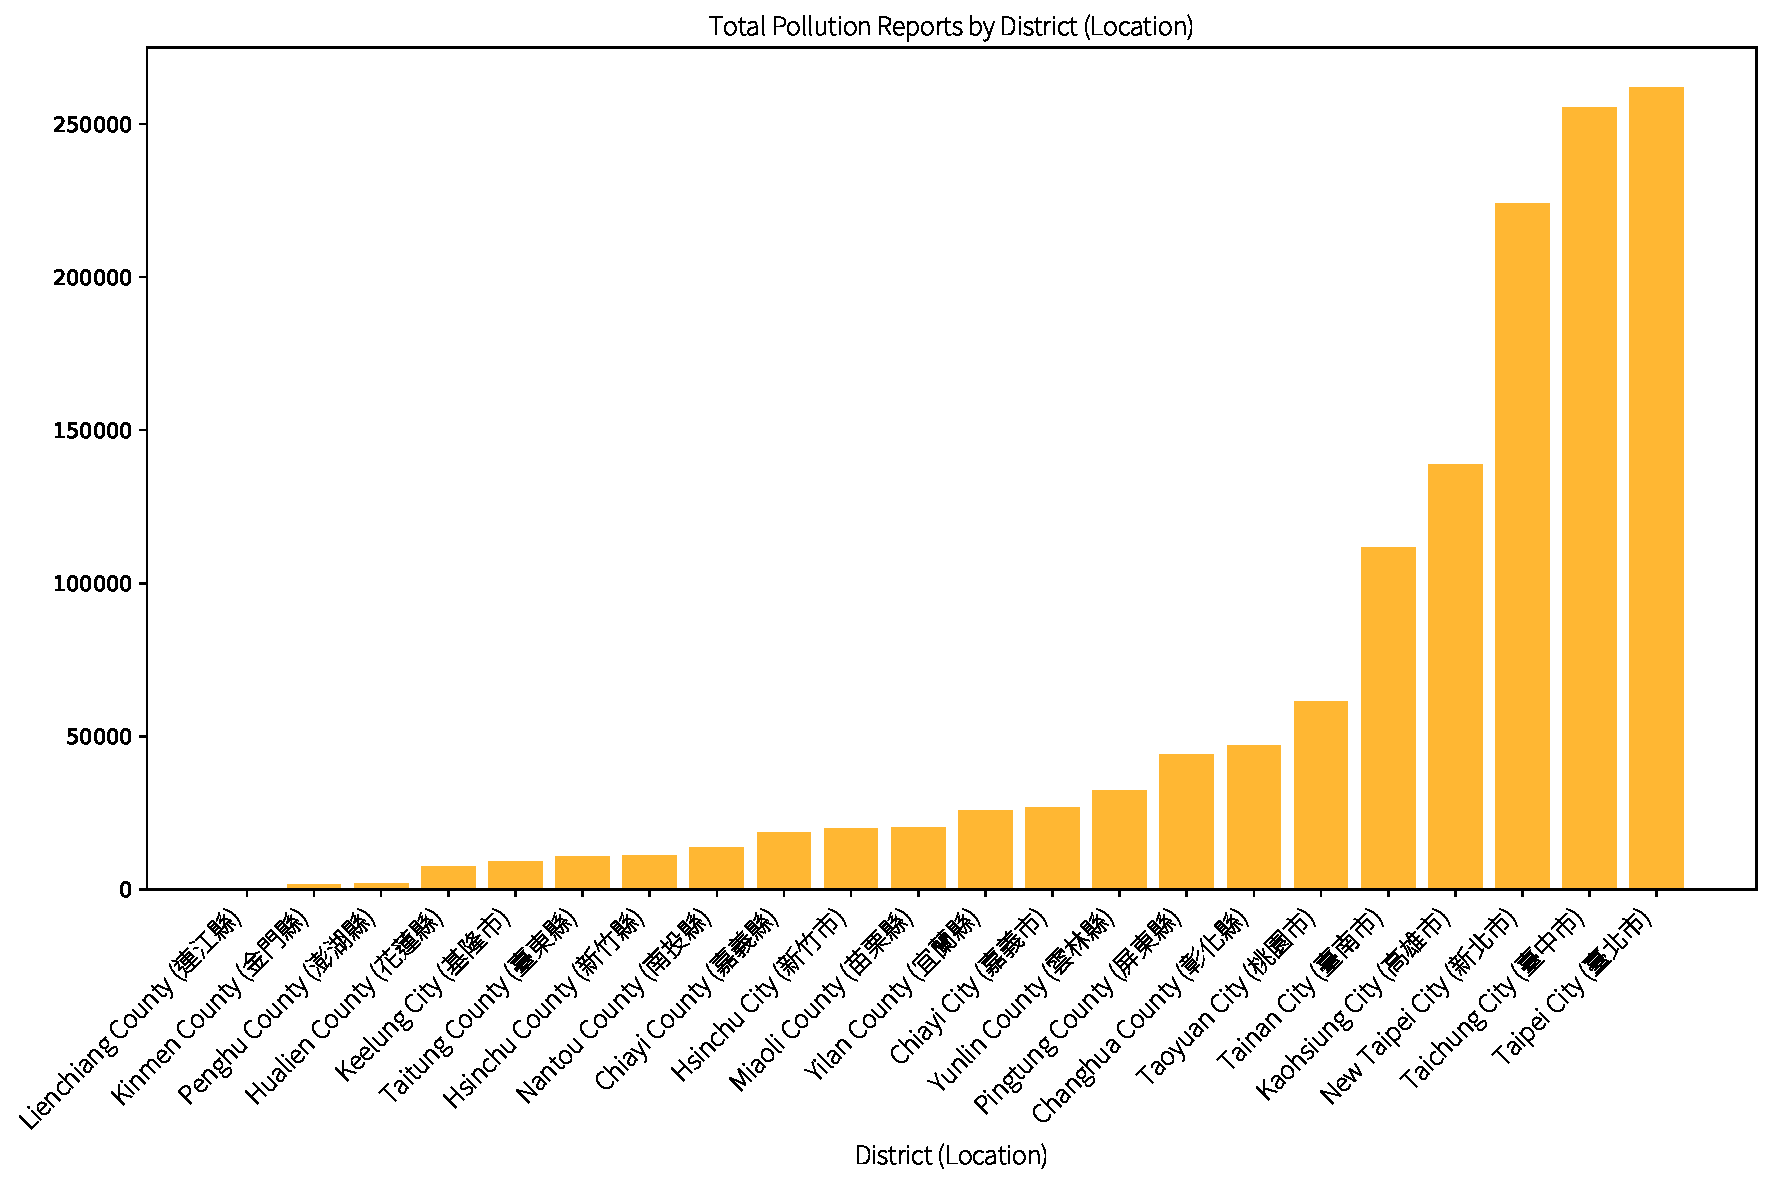
\includegraphics[keepaspectratio]{_thesis-nocite_files/figure-pdf/fig-tw-poll-reports-output-1.pdf}}

}

\caption[Pollution Reports in Taiwan by
County]{\label{fig-tw-poll-reports}Pollution Reports in Taiwan by
County}

\end{figure}%

Pollution Reports in Taiwan by District.

\begin{figure}

\centering{

\centering{

\begin{verbatim}
<Figure size 3600x2400 with 0 Axes>
\end{verbatim}

}

\subcaption{\label{fig-tw-poll-reports-stack-1}Pollution Reports in
Taiwan by District}

\centering{

\pandocbounded{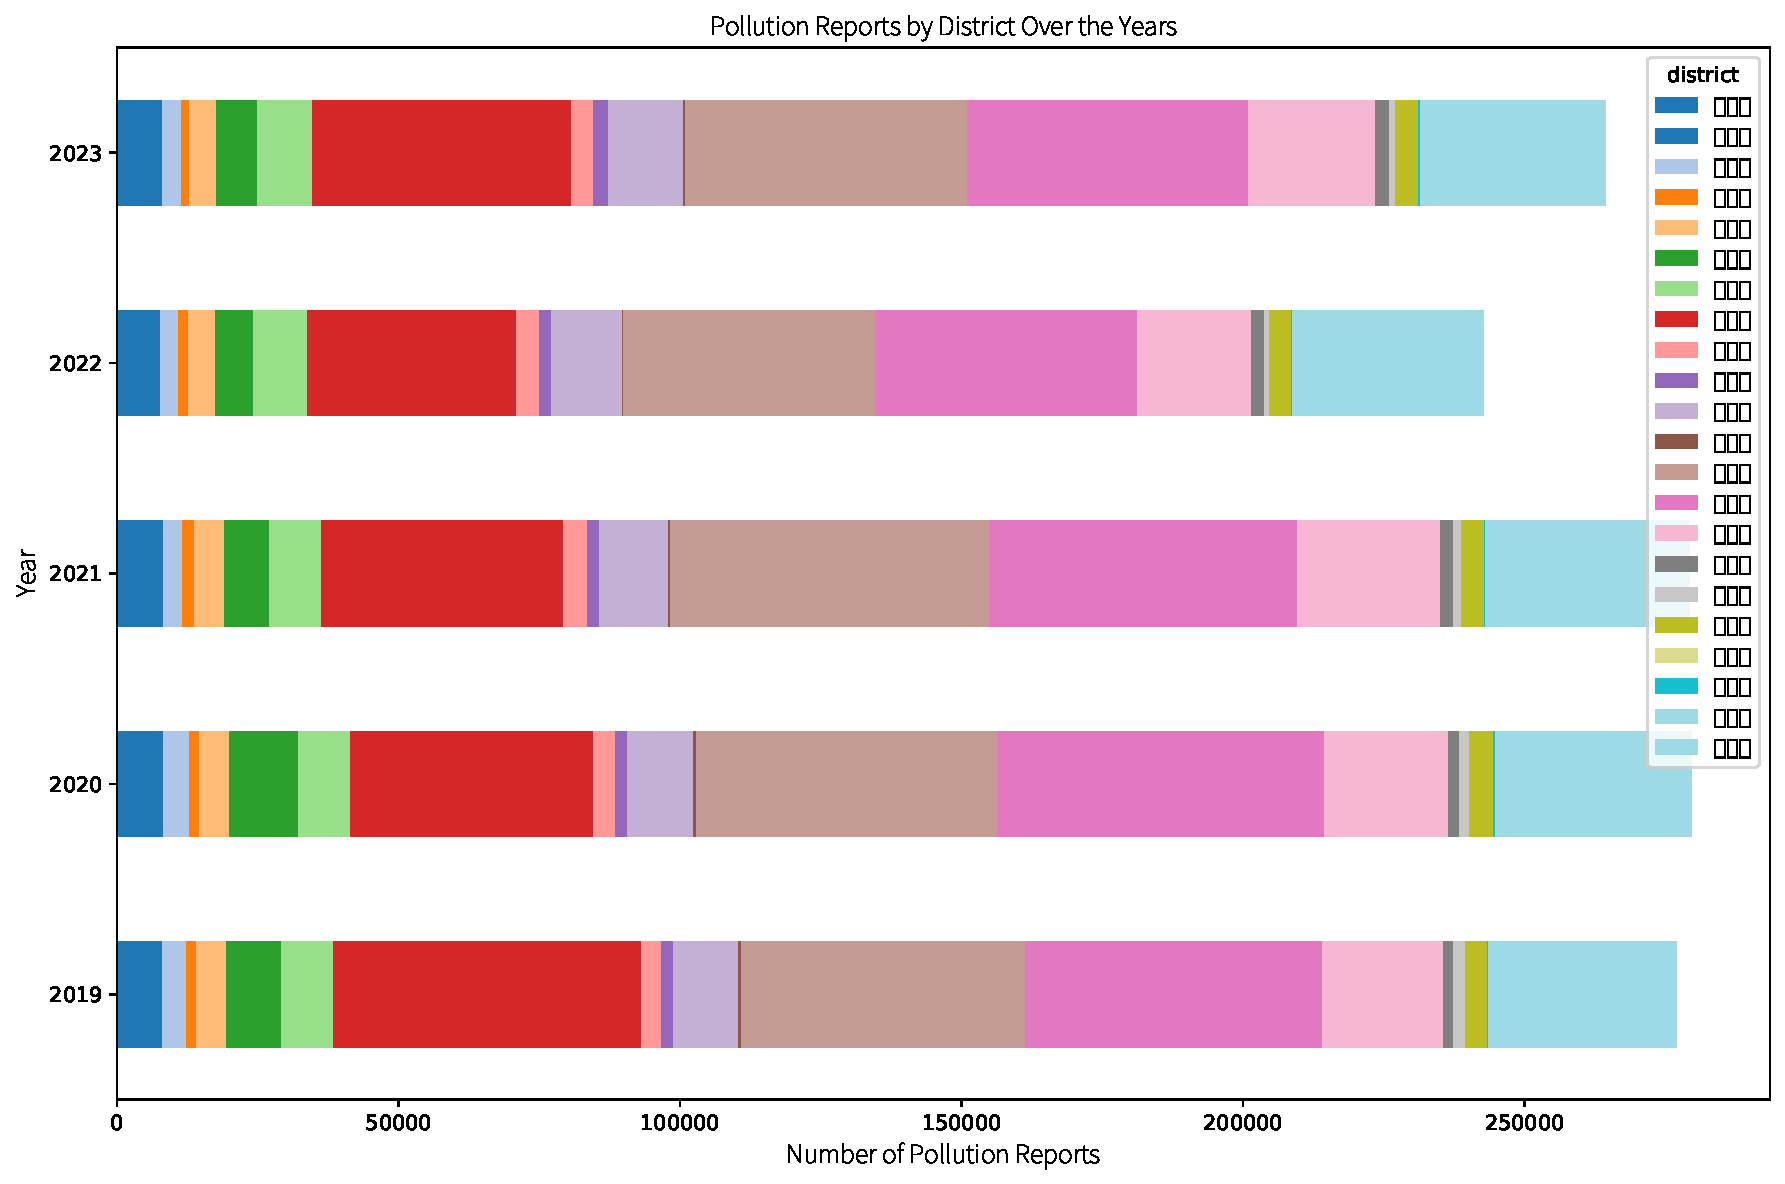
\includegraphics[keepaspectratio]{_thesis-nocite_files/figure-pdf/fig-tw-poll-reports-stack-output-2.pdf}}

}

\subcaption[Pollution Reports in Taiwan by
District]{\label{fig-tw-poll-reports-stack-2}}

}

\caption{\label{fig-tw-poll-reports-stack}}

\end{figure}%

Health and sustainability are inextricably linked. ``Human health is
central to all sustainability efforts.'', \emph{``All of these (food,
housing, power, and health care), and the~stress~that the lack of them
generate, play a huge role in our health''} (Sarah Ludwig Rausch \& Neha
Pathak, 2021).

(Abu El Kheir-Mataria \& Chun, 2025) finds warming climate in the MENA
region (Middle East and North Africa) increases cancer risk in women,
mediated through air pollution and other environmental stressors.

Clean air is a proposed as a \emph{human right} (Baroness Jones of
Moulsecoomb \& Caroline Lucas, 2023), yet air pollution is widespread
around the planet, with 99\% of Earth's human population being affected
by bad air quality that does not meet WHO air quality guidelines,
leading to health problems linked to 6.7 million \emph{premature deaths}
every year (World Health Organization, 2022). Air pollution is linked to
cancer incidence. In Taiwan, South Korea, and England, groundbreaking
research by (Lim et al., 2022) analyzed over 400000 individuals
establishes exposure to 2.5μm PM (PM2.5) air pollution as a \emph{cause
for lung cancer.} In (Hannah Devlin, 2022), professor Tony Mok, of the
Chinese University of Hong Kong explains it plainly, which I want to
quote here in verbatim:

\begin{quote}
\emph{``We have known about the link between pollution and lung cancer
for a long time, and we now have a possible explanation for it. As
consumption of fossil fuels goes hand in hand with pollution and carbon
emissions, we have a strong mandate for tackling these issues -- for
both environmental and health reasons.''} - (Hannah Devlin, 2022)
\end{quote}

The main way to combat air pollution is through policy interventions.
(MARIA LUÍS FERNANDES, 2023) the EU has legislation in progress to curb
industrial emissions. If legislation is in place, causing bad air
quality can become bad for business. In China, (Gu et al., 2023) links
air pollution to credit interest rates for business loans; companies
with low environmental awareness and a history of environmental
penalties pay 12 percent higher interest rates. In France, (Bouscasse et
al., 2022) finds strong health and economic benefits across the board
from air pollution reduction.

Likewise to the lack of clean air, lack of access to sufficient clean
water and water pollution are issues in several places around the world;
globally, 4.4 billion people only have access to water that's not safe
for drinking (Soliman, 2024). Even in wealthy countries like the US,
with increasing situations of water scarcity and drought due to climate
change, issues of water ownership become increasingly dire. (Koch, 2022;
Naishadham, 2023b) describes a fight in the US over water usage rights
in Arizona, where Fondomonte, a subsidiary of a Saudi Arabian company
that grows a water-hungry crop alfalfa, exacerbating the local water
crisis by using large amounts of public water, leading to public outcry
and being sued for ``public nuisance'' for its excessive groundwater
pumping, and finally cessation of its lease and operations on state
land; but still continuing operations on private land (Naishadham,
2023a; {``Saudi Firm That Grows Hay in {California} and {Arizona} to
Lose Farm Leases over Water Issue,''} 2023).

Water quality is highly dependent on competent governance. For example,
in the U.S., the national government recently rolled back rules for
water safety, which had only been implemented last year, to protect the
consumer from per- and polyfluoroalkyl substances (PFAS) (Trager, 2025).
Once pollution is in the environment, cleaning it up is very expensive.
For instance, in France, where storm water washed pollution into the
waterways feeding into the Seine river, making it unsuitable for
swimming, the city of Paris invested 1.4 Billion Euros to create a
massive underground reservoir and a water cleaning system by the opening
of the Paris Olympics in 2024 - and still the water quality would be
variable based on rain incidence (Walt, 2023).

Water and soil pollution are highly connected, as water flows through
soil. In Saudi Arabia, (Picó et al., 2023) used wild and ruderal plants
as bioindicators to detect pollution of air, water and soil,
specifically anthropogenic pollution, pharmaceuticals, pesticides, and
other industrial chemicals, concluding both Abha and Riyadh showed
notable levels of pollutants while Riyadh (a city with more industry)
showed higher levels of pollution.

Improved farming practices directly improve soil structure (reducing
runoff and contamination) and water retention, thereby mitigating both
soil degradation and water pollution. Participants in the 2023 Baltic
Sea Action Group for the EIT Food Regenerative Agriculture project
(which so far has trained over 1200 farmers and 160 farmers advisory
groups in regenerative practices), highlighted practical
soil‐restoration methods in their respective countries: applying
\emph{biochar} on pilot plots in the Czech Republic increased water
retention by up to 20\%, no‐tilling and cover‐cropping practices in
Hungary boosted insect‐species counts by 15 points, and adopting
regenerative crop rotations in Bulgaria cut synthetic fertilizer use by
25\%; one of the challenges remains consumer awareness: only 12\% of
consumers in Central and Eastern Europe currently recognize the
``regenerative'' label - awareness must grow to drive demand (Baltic Sea
Action Group, 2023).

A practical example of the interconnection between water pollution,
agriculture, architecture, and extreme weather, are bioswales, which
help catch storm debris and reduce water pollution. In Taiwan, (劉大正,
2010) showed that grass swales increase infiltration, reduce runoff, and
improve downstream water quality, helping stabilize slopes via enhanced
drainage (Taiwanese landscape is very mountainous, with); in a follow-up
field trial at a National Highway in Gangshan, grass swales consistently
trapped sediments and adsorbed heavy metals from highway runoff before
those pollutants could reach nearby waterways.

The above examples from around the world suggest that
\emph{``regenerative''} is not just a buzzword or wishful thinking -
instead, it maps to a set of concrete practices and approaches to
improve the condition of the living environment under threat from
pollution.

\subsubsection{Climate Disaster Preparedness: Extreme Weather
Resilience}\label{climate-disaster-preparedness-extreme-weather-resilience}

The Word Economic Forums Global Risks Report 2024 paints a bleak picture
of the future with expectations of increased turbulence across the board
based on a survey of over 1400 topic experts (World Economic Forum,
n.d.). Global warming specifically increases the risk of disasters and
extreme weather events; the US Global Change Research Program presented
a comprehensive report to the US Congress, which links disaster-risk
directly to global warming; for examples increased wildfires damage
property, endanger life and reduces \emph{air quality,} which in effect
increases health challenges (\emph{Fifth {National Climate Assessment}},
2023). Warming global climate has concrete effects on daily life. Warmer
climate helps viruses and fungi spread (Press, 2023). (Williams \&
Joshi, 2013) higher CO\textsubscript{2}eq concentrations in the air can
cause more turbulence for flights. As extreme temperatures are
increasingly commonplace, with observed changes in heatwaves, there's
increased risk of wildfires (Perkins-Kirkpatrick \& Green, 2023; Volkova
et al., 2021), while flood risk mapping might lower property prices in
at risk areas (Sherren, 2024). Summers of 2022 and 2023 were the hottest
on record so far, with extreme heat waves recorded in places around the
world (Douglas, 2023; Falconer, 2023; National Oceanic and Atmospheric
Administration (NOAA), U.S. Department of Commerce, 2023; NOAA National
Centers for Environmental Information, 2023; Serrano-Notivoli et al.,
2023; Venturelli et al., 2023).

The part of Earth where the \emph{human climate niche} is becoming
smaller (McKibben, 2023). As temperatures rise, certain cities may
become uninhabitable for humans (CBC Radio, 2021). The summer of 2023
saw extensive wildfires in Spain, Canada, and elsewhere; rapidly moving
fires destroyed the whole city of Lāhainā in Hawaii (Anguiano, 2023). In
California, (Jerrett et al., 2022) says, \emph{``{[}w{]}ildfires are the
second most important source of emissions in 2020''} and \emph{``negate
reductions in greenhouse gas emissions from other sectors.''} Some parts
of South America have seen summer heat \emph{in the winter}, with
heatwaves with temperatures as high as 38 degrees (Livingston, 2023).

In Taiwan disaster risk and hazard mapping is well-developed, with early
warning systems, and comprehensive response preparedness - and painful
experiences - instrumental to saving lives (Y.-J. Tsai et al., 2021).
Intensifying storms forming near coastlines, can be expected with
\emph{``{[}c{]}hanges to tropical cyclone trajectories in Southeast Asia
under a warming climate''} (Garner et al., 2024). The situation on the
Pacific and Atlantic oceans is not dissimilar, with
\emph{``{[}o{]}bserved increases in North Atlantic tropical cyclone peak
intensification rates''} (Garner, 2023).

In the Philippines, with increasing extreme weather events,
\emph{``businesses are more likely to emerge in areas where
infrastructure is resilient to climate hazards''} (Y. Cheng \& Han,
2022). Across several case studies, (Fabris \& Luburić, 2022) discusses
vulnerable sectors from agriculture to transport, under threat from
extreme weather events, such as floods, heatwaves, droughts, and storms
impact human health: societal development and economic growth should be
realistic on planning for weather-related impacts.

Climate-related disasters can spur action as extreme weather becomes
visible to everyone. After large floods in South Korea in July 2023 with
many victims, president Joon promised to begin taking global warming
seriously and steer the country towards climate action (AFP, 2023; Al
Jazeera, 2023; Web, 2023). South Korea has a partnership with the
European Union (European Commission, 2023a).

\subsection{Financialization of Nature vs Sacred Value: Scaling Up
Sustainable
Action}\label{financialization-of-nature-vs-sacred-value-scaling-up-sustainable-action}

There are 2 main approaches to protecting nature:

\def\pandoctableshortcapt{Economics of Nature Commodification vs Sacred
Economics}

\begin{longtable}[]{@{}
  >{\raggedright\arraybackslash}p{(\linewidth - 2\tabcolsep) * \real{0.3611}}
  >{\raggedright\arraybackslash}p{(\linewidth - 2\tabcolsep) * \real{0.6389}}@{}}
\caption[Economics of Nature Commodification vs Sacred
Economics]{Economics of Nature Commodification vs Sacred
Economics}\tabularnewline
\toprule\noalign{}
\endfirsthead
\endhead
\bottomrule\noalign{}
\endlastfoot
\textbf{Economics of Nature Commodification} & \textbf{Economics of the
Sacred} \\
Measure and assign monetary value to nature. & Nature is Sacred - such
as are religious holy places - and can't be touched (Eisenstein, 2011,
2018) \\
\end{longtable}

\let\pandoctableshortcapt\relax

Whether we should put a price on nature (or is it time to leave
utilitarian environmentalism behind?) is still openly debated, with
pro-financialization voices arguing assigning monetary figures to
nature's benefits legible to policymakers and markets, channeling large
sums into conservation (e.g.~carbon/biodiversity credits), while critics
argue monetary metrics flatten relational, cultural and intrinsic values
of ecosystems into exchange-value and commoditize nature, which may
legitimize offsetting schemes that displace rather than prevent damage
(Leverhulme Centre for Nature Recovery, 2023).

Ecosystem services literature defines a ``Nature's Contributions to
People'' framework, originally proposed by the Intergovernmental
Science-Policy Platform on Biodiversity and Ecosystem Services (IPBES).
(Díaz et al., 2018). (Muradian \& Gómez-Baggethun, 2021) critically
assesses the framework, arguing utilitarian and anthropocentric views of
the ecosystem services concept perpetuates problematic dualisms (humans
and nature are separate) - and call for a new approach centered on
ecology.

\def\pandoctableshortcapt{Defining Ecosystem Services Concepts}

\begin{longtable}[]{@{}l@{}}
\caption[Defining Ecosystem Services Concepts]{Defining Ecosystem
Services Concepts from (Leverhulme Centre for Nature Recovery,
2023)}\tabularnewline
\toprule\noalign{}
\endfirsthead
\endhead
\bottomrule\noalign{}
\endlastfoot
9 Steps Towards Defining Ecosystem Services \\
Identify ecosystem functions \\
Quantify ecosystem functions \\
Identify ecosystem services \\
Quantify ecosystem services \\
Quantify financial value of ecosystem services \\
Assign property rights \\
Create ecosystem service markets \\
Commodify nature \\
\end{longtable}

\let\pandoctableshortcapt\relax

A practical example of ecosystem services becoming a common language
comes from (Z. Zhang et al., 2023) who proposes integrating ecosystem
services conservation into urban planning, so biodiversity could become
part of city planning. Another example is tourism, a large industrial
sector which relies on ecosystem services (L. Li et al., 2023). In
Taiwan, (T. H. Lee et al., 2021) developed a framework of indicators to
assess sustainable tourism.

\subsubsection{Ecological Restoration: Damaged Ecosystems, Agroforestry
\&
Permaculture}\label{ecological-restoration-damaged-ecosystems-agroforestry-permaculture}

The concept of how a public resource is over-used until breaking down as
each user only bears a fraction of the cost - know as \emph{tragedy of
the commons} - was described by the ecologist Garrett Hardin in 1968
(Hardin, 1968; Lopez et al., 2022; Meisinger, 2022; Murase \& Baek,
2018). When so many systems are broken, some argue sustainability is not
enough and we should work on \emph{regeneration} of natural habitat. The
UN announced 2021-2030 the Decade on Ecosystem Restoration, which
includes a wide range of regenerative action (Fischer et al., 2021). For
instance, (Han \& Chen, 2022) identifies nature-based solutions ``land
re-naturalization (such as afforestation and wetland restoration)''

\def\pandoctableshortcapt{Regenerative Actions}

\begin{longtable}[]{@{}l@{}}
\caption[Regenerative Actions]{Non-Exhaustive list of Regenerative
Actions from (Han \& Chen, 2022)}\tabularnewline
\toprule\noalign{}
Non-Exhaustive list of Regenerative Actions \\
\midrule\noalign{}
\endfirsthead
\toprule\noalign{}
Non-Exhaustive list of Regenerative Actions \\
\midrule\noalign{}
\endhead
\bottomrule\noalign{}
\endlastfoot
Afforestation \\
Wetland restoration \\
 \\
\end{longtable}

\let\pandoctableshortcapt\relax

The organic food and drink market is growing worldwide, with gross sales
in 2019 totaling over 106 billion euros, albeit being a small percentage
of total food industry (Gamage et al., 2023). Growing organic food poses
many challenges, which farmers need to adapt to, in order to participate
in regenerative food systems. One approach is growing food forests, also
known as agroforestry, which integrates farming into natural
environments, achieving CO\textsubscript{2}eq storage in the soil
through agriculture and forestry using agroecological practices.

In Ireland, (Irwin et al., 2023) studied dairy farmers' willingness to
plant trees to increase vegetation cover on their land, finding that
economic incentives alone are insufficient, and support in the form of
advisory and education is needed. Similarly, in the Brazilian Amazon
rainforest (Yadav et al., 2023) finds the active participation of the
local community in planning permaculture practices, enhances their
acceptance and effectiveness. In Bangladesh, (Ruba \& Talucder, 2023)
found agroforestry plays an active role in achieving the country's
Sustainable Development Goals (SDGs), including zero hunger, climate
action, mitigating climate change impacts through CO\textsubscript{2}eq
sequestration, life on land through biodiversity conservation and
improving soil fertility, yet is hindered by the lack of policy support
and educational level of the farmers. In the Baltic Sea region in
North-Eastern Europe and Central Europe face similar challenges, (Baltic
Sea Action Group, 2023) pointing out farmers' traditional mindset as the
biggest obstacle, describing the paradigm shift from extractive farming
to regenerative agriculture, using techniques such as no-till farming,
which reduces soil erosion and improve soil health by reducing synhetic
imputs; yet, it's not only a single practice that is enough,
regenerative agriculture is a holistic approach and agroecology
education programmes need to be comprehehnsive.

(G. Low et al., 2023) further studies how agroforestry deep integration
into food value chains unlocks opportunities for recognition and rewards
from economic actors in the network, underlining how complex and
knowledge-heavy nature of value-capture, calling for further
standardization of practices to reward sustainability practices and
ecosystem services. The challenge lies in that bioeconomy is not
inherently sustainable and may put biodiversity at risk, depending on
the level of industrialization of agriculture and specific practices,
which require deep knowledge and understanding of natural and artificial
interactions the ecological systems; the authors advocate for a precise
distinction between extractive and regenerative practices in
\emph{``bioeconomy''} (Ollinaho \& Kröger, 2023). Finally, taking Brazil
as and example, (De Queiroz-Stein \& Siegel, 2023) argues for an
integration of competing and conflicting bioeconomy policies, in order
to achieve the goals of a sustainable bioeconomy.

Svalbard Seed Vault is an example of seed conservation to safeguard
biodiversity by storing backup seeds of plants from around the world in
cold storage (Asdal \& Guarino, 2018; Westengen et al., 2013). Since its
opening in 2008, the storage solution provided by the Norwegian
government has stored seeds from 123 gene banks in 85 countries around
the world ({``Arctic Doomsday Seed Vault Gets More Than 14,000 New
Samples,''} 2025; The Norwegian Ministry of Agriculture and Food, 2025).
(Vitaletti, 2025) proposes using a blockchain-based lottery system to
storage seeds in local refrigerators, in order to enhance resilience and
ensure survival of seeds, by storing seeds in many locations.

\subsubsection{Energy: Climatech, Renewables, and Decarbonization
Pathways}\label{energy-climatech-renewables-and-decarbonization-pathways}

Globally, 34\% of all emissions come from energy production (US EPA,
2016), making it the key sector to require innovate for reducing carbon
emissions. The International Energy Agency's (IEAs), \emph{``Tracking
Clean Energy Progress''} report on 50 distinct decarbonization enablers
and finds that only 3 components - solar PV, PV electric vehicles, and
building lighting - are on track with the net-zero by 2050 scenarios,
while 28 need more effort and 22 are ``not on track'' (IEA, 2023b).

Geopolitical situations can affect technology adoption; after Russia's
war in Ukraine, Europe needed to quickly reduce consuming cheap Russian
fossil fuel energy (in the form of gas) (Bonasia, 2024). In 2024, for
first time in Europe, renewables in the form of wind and solar energy
surged past production of fossil fuels (Beer, 2024; Graham \& Fulghum,
2024). Meanwhile, China is experiencing a solar installation rush before
a deadline set by a new renewable pricing policy; from January to April
2025, a record-breaking 105 gigawatts (GW) of solar capacity was
installed, bringing the total solar power close to 1 Terawatt, predicted
to make solar power China's main energy source in 2026(Carrie Xiao,
2025; L, 2025a; Redazione, 2025; Weaver, 2023; Y. Zhu, 2023).

(Gaure \& Golombek, 2022) simulate a CO\textsubscript{2} free
electricity generation system in the European Union where \emph{``98\%
of total electricity production is generated by wind power and solar;
the remainder is covered by a backup technology.''} The authors
stipulate it's possible to power the EU without producing
CO\textsubscript{2} emissions.

EU's energy mix in 2024:

\begin{figure}

\centering{

\pandocbounded{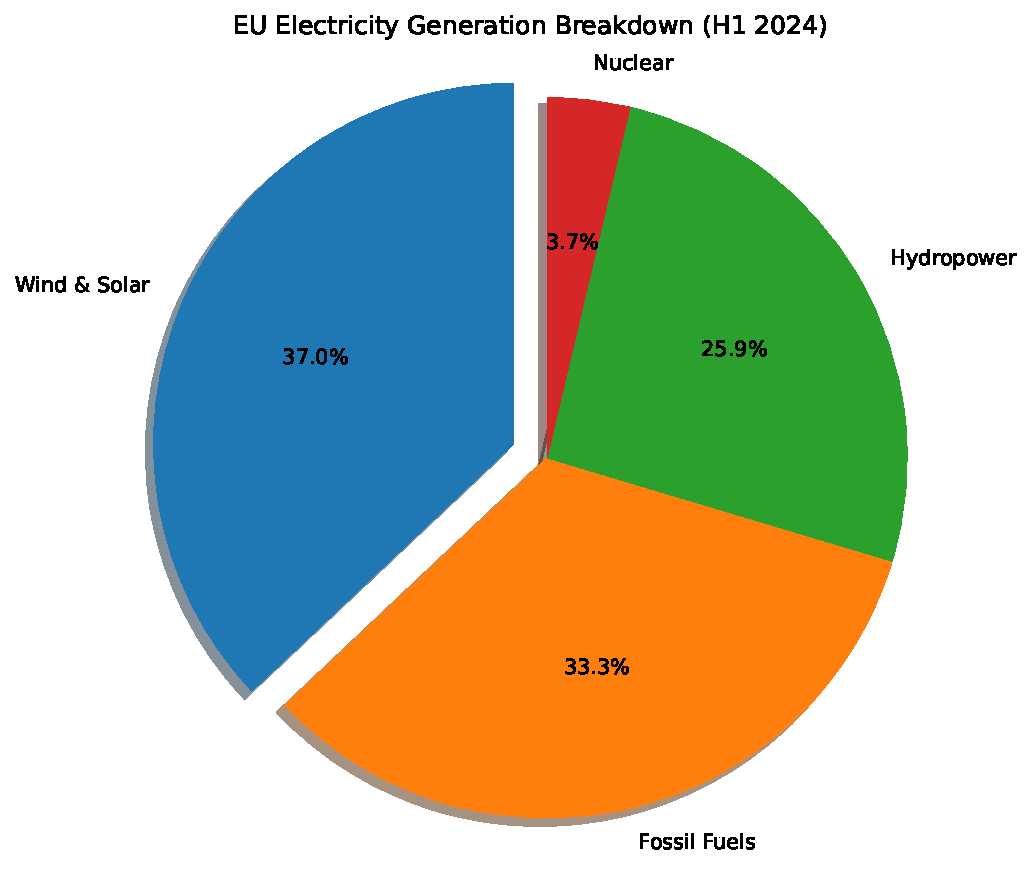
\includegraphics[keepaspectratio]{_thesis-nocite_files/figure-pdf/fig-eu-energy-brakdown-output-1.pdf}}

}

\caption[The EU's Energy Production
Breakdown]{\label{fig-eu-energy-brakdown}The EU's Energy Production
Breakdown}

\end{figure}%

Wind and solar energy overtook fossil energy in Europe:

\begin{figure}

\centering{

\pandocbounded{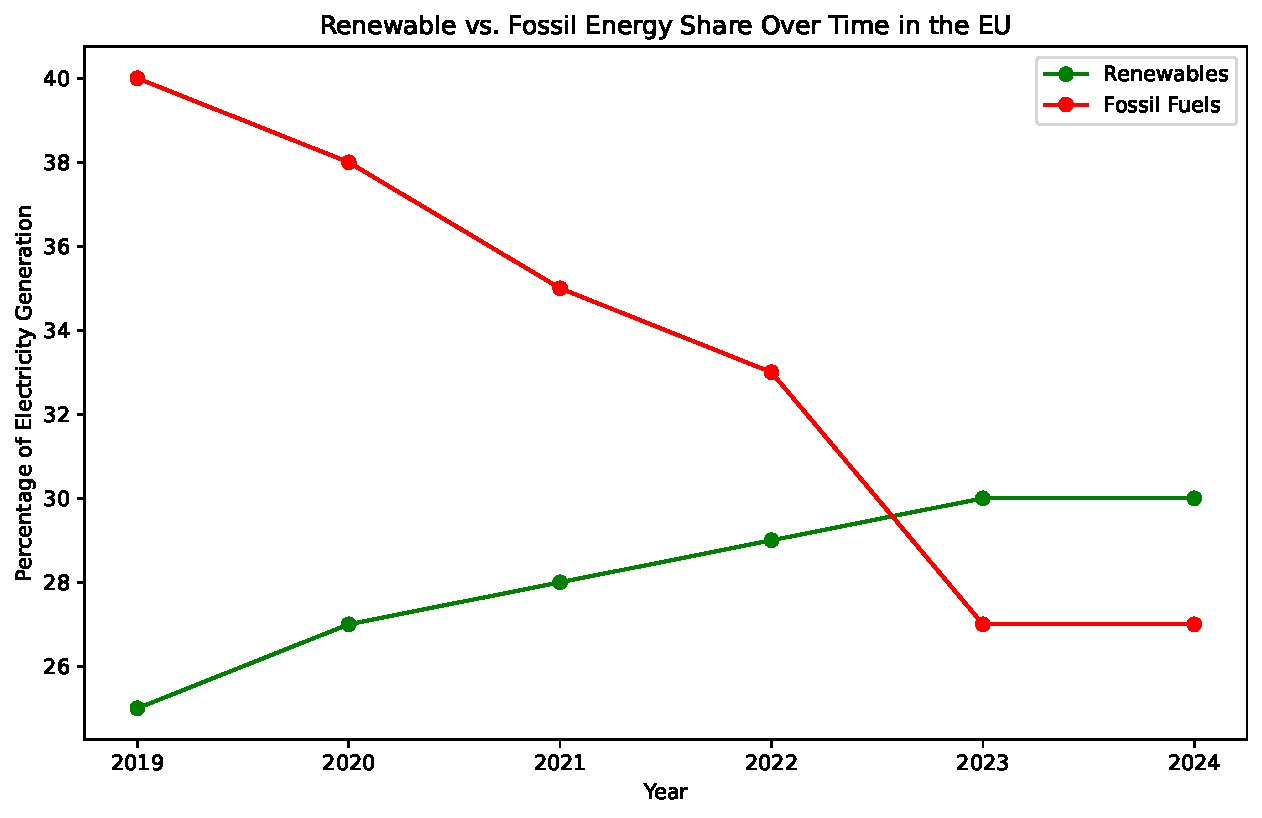
\includegraphics[keepaspectratio]{_thesis-nocite_files/figure-pdf/fig-eu-renew-vs-fossil-output-1.pdf}}

}

\caption[The EU's Renewables vs Fossil
Energy]{\label{fig-eu-renew-vs-fossil}The EU's Renewables vs Fossil
Energy}

\end{figure}%

Globally, renewables also overtook fossil fuels (IEA, 2024):

\begin{figure}

\centering{

\pandocbounded{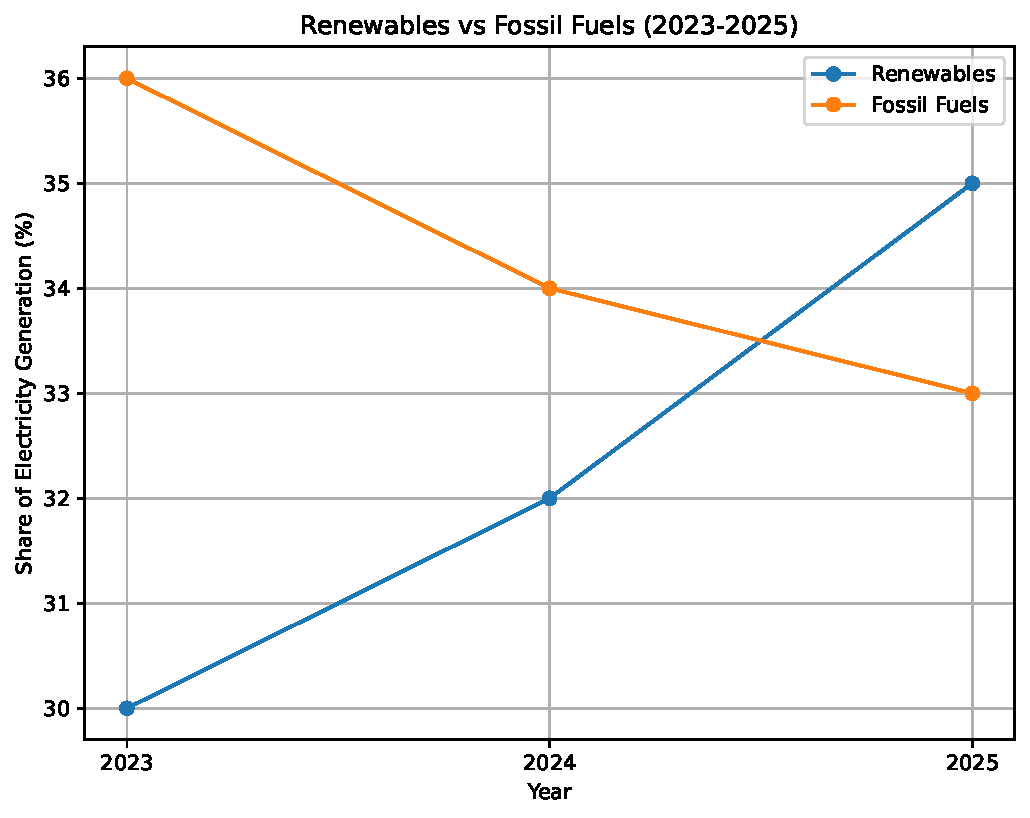
\includegraphics[keepaspectratio]{_thesis-nocite_files/figure-pdf/fig-global-renew-vs-fossil-output-1.pdf}}

}

\caption[Global Renewables vs Fossil
Energy]{\label{fig-global-renew-vs-fossil}Global Renewables vs Fossil
Energy}

\end{figure}%

Meanwhile, reduction in coal-power was also possible. Coal is a large
CO\textsubscript{2}eq emitter.

\begin{figure}

\centering{

\pandocbounded{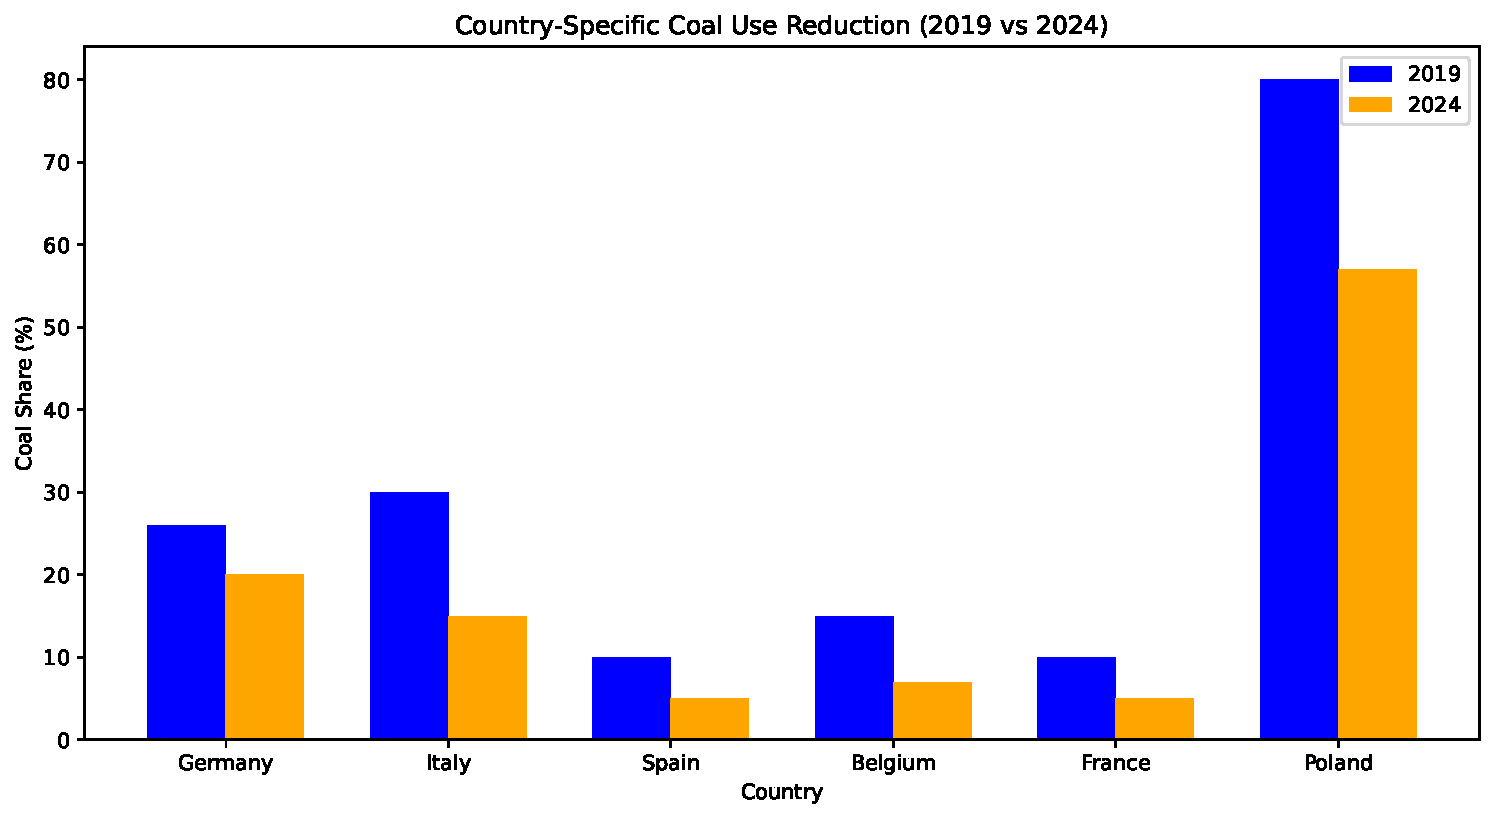
\includegraphics[keepaspectratio]{_thesis-nocite_files/figure-pdf/fig-renew-vs-fossil-output-1.pdf}}

}

\caption[The EU's Reduction of Coal
Energy]{\label{fig-renew-vs-fossil}The EU's Reduction of Coal Energy}

\end{figure}%

\begin{figure}

\centering{

\pandocbounded{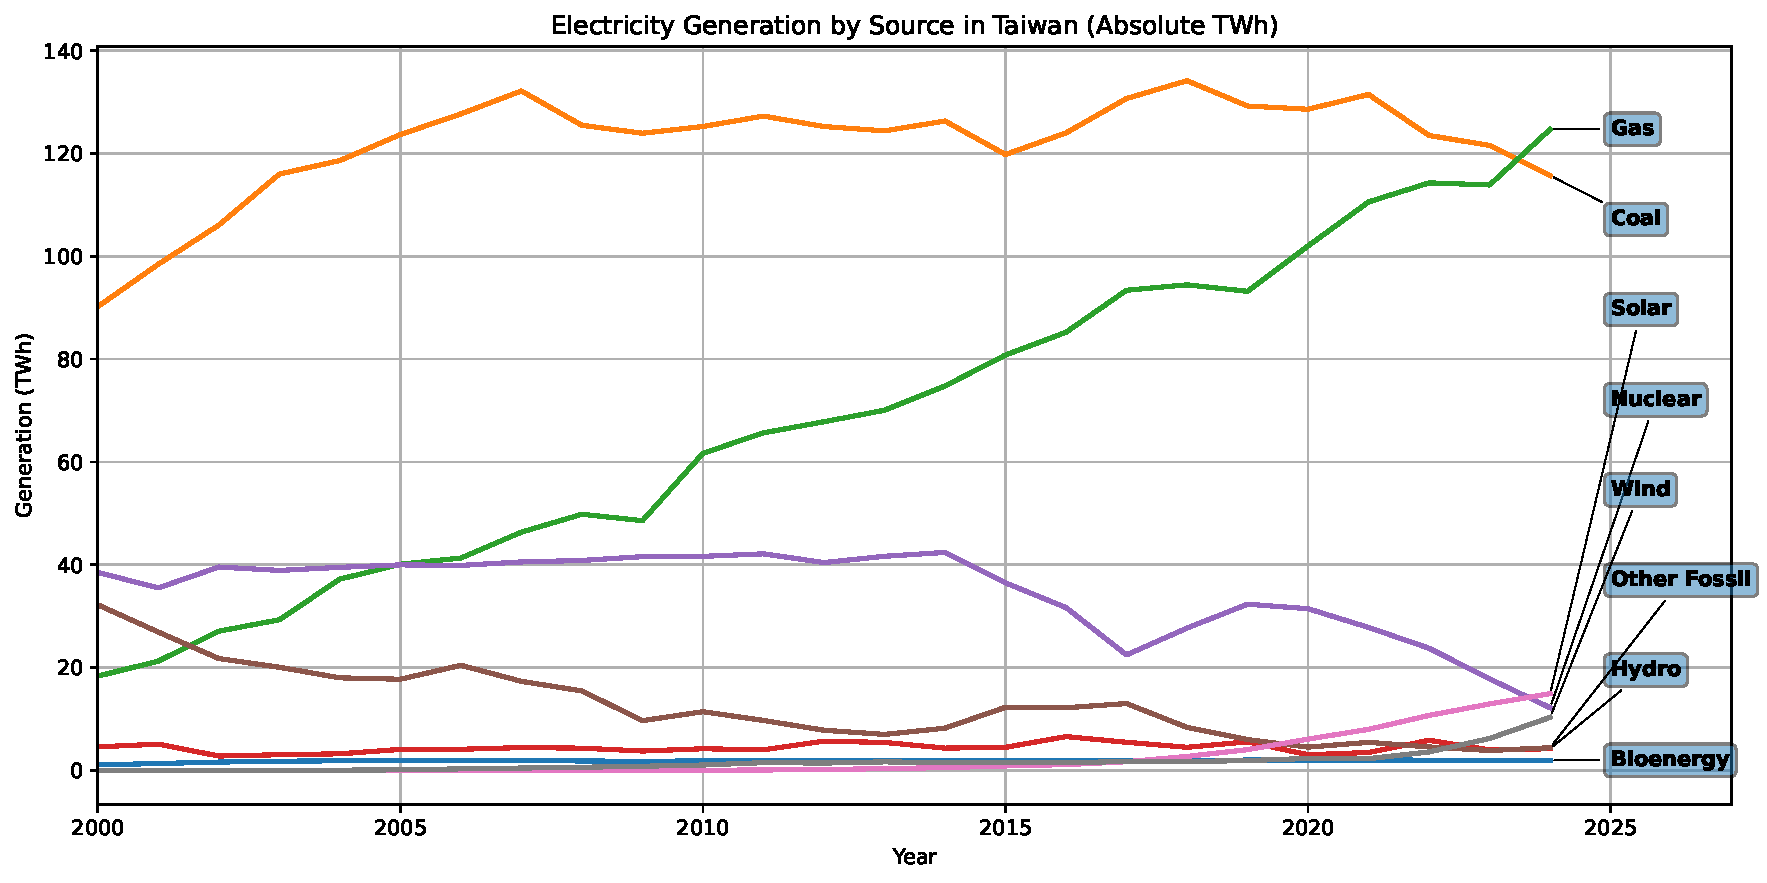
\includegraphics[keepaspectratio]{_thesis-nocite_files/figure-pdf/fig-tw-energy-prod-output-1.pdf}}

}

\caption[Taiwanese Energy
Production]{\label{fig-tw-energy-prod}Taiwanese Energy Production}

\end{figure}%

Beyond electricity and heat, the chemical sector is a massive
CO\textsubscript{2}eq source. (Lange, 2021) reports the petrochemical
industry uses about 10\% of global fossil carbon as feedstock and
another 7\% to power its processes, producing some 400Mt of base
chemicals each year, 36\% of which becomes packaging; the cradle-to-gate
CO\textsubscript{2}eq emissions for base chemicals are roughly 1--2.5kg
CO\textsubscript{2}eq per kg or 5t CO\textsubscript{2}eq per tonne of
plastic, when including use and end-of-life, the entire lifecycle
emissions are 1.7Gt CO\textsubscript{2}eq (∼4\% of all anthropogenic
emissions) per year; a true circular-carbon economy would require
renewable carbon feedstocks (e.g.~biomass or CO\textsubscript{2}-derived
monomers), electrified green heat, closed-loop catalytic recycling of
molecular building blocks, and modular low-temperature reactors to slash
energy demand.

Large technology conglomerates and newly founded startups alike are
working in the climate solutions space (often referred to as
\emph{climatech} by the media), have proposed a range of approaches to
CO\textsubscript{2} reduction in the Earth's atmosphere. These
technologies include several types of \emph{carbon capture}, directly
from the air (direct air capture or DAC), from the source of pollution,
such as using high--performance filters on factory chimneys, as well as
nature-based solutions such as large scale tree planting using drones.
Each technology has their own pros and cons. For instance, (Vitillo et
al., 2022) illustrates how direct air capture of CO\textsubscript{2} is
difficult because of low concentration and CO\textsubscript{2} capture
at the source of the emissions is more feasible. (Cleantech Group, 2023)
profiles 100 innovators across agriculture, food, energy, mobility, and
waste that Cleantech Group judges most likely to enable a future with
sub-2 degrees warming. Overall, considering pathways to carbon drawdown
finds considerable uncertainty exists among experts which
CO\textsubscript{2}eq reduction among nature- and technology-based
methods are the most effective (S. Low et al., 2022).

\subsubsection{Individual Action}\label{individual-action}

Sometimes individual environmental (climate) action \emph{does matter}
and can come at great personal cost, even loss of life. EJAtlas tracks
environmental justice cases around the world, where human stakes are
very high. See (Joan Martinez-Alier, 2021; J. Martinez-Alier et al.,
2022; Scheidel et al., 2020) for coverage of extreme cases of risk
environmental activists must endure.

However, for most of us individual climate action is \emph{ineffective}.
The effect of individual climate action such as \emph{choosing a more
sustainable product} is so limited to be next to meaningless. For
individual consumer choices to make a difference, they need to be
\emph{aggregated} into a movement, collective action with scale,
influence, and visibility.

There is no single solution to the environmental crisis. Given the
enormity of environmental degradation, many different approaches are
needed. This chapter documents some of the ongoing work which a
sustainability companion could assist college students get involved
with.

While the scale of climate change is too big for individual action to
make a difference, individual action can foster hope and a sense of
collective responsibility (Nature, 2020).

\newpage

\section{Design}\label{design}

\begin{figure}[H]

{\centering \pandocbounded{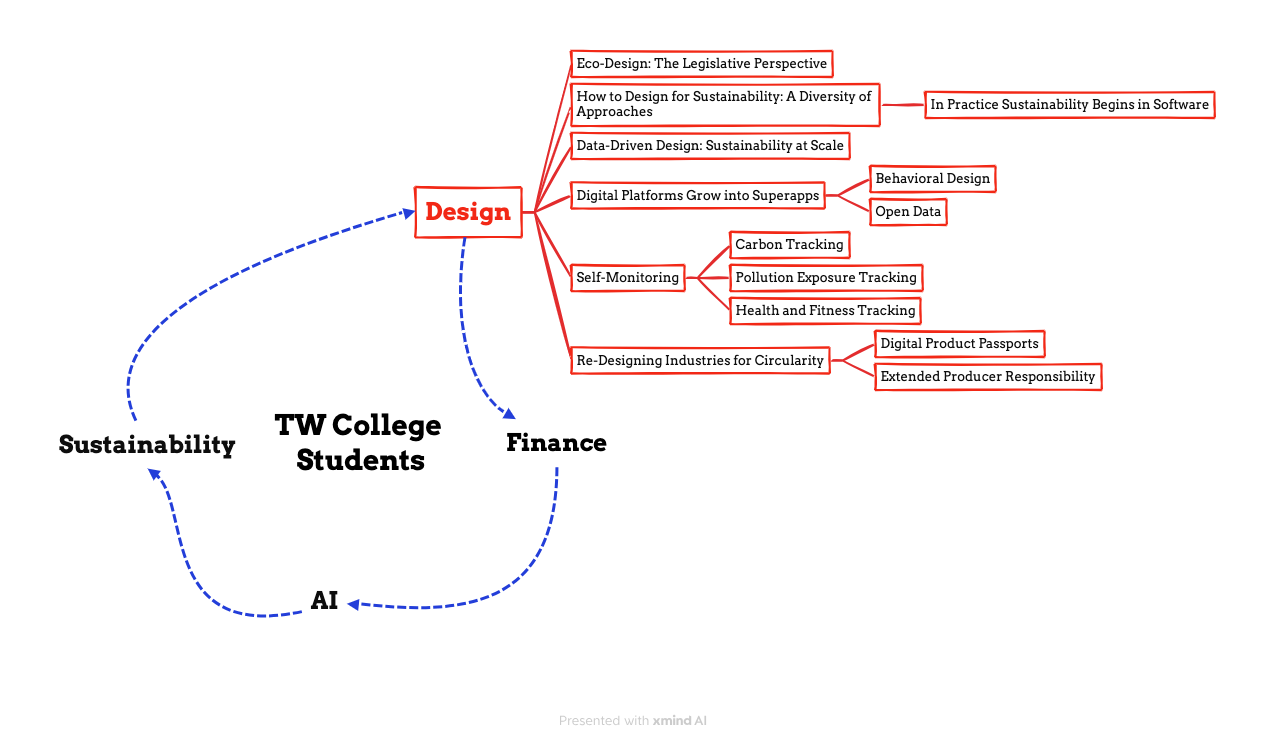
\includegraphics[keepaspectratio]{./images/design/abstract-design.png}}

}

\caption{Visual abstract for the design chapter}

\end{figure}%

Designers have been battling complexity since the beginning of design.
Industrial designer Dieter Rams famously said in the 1970s \emph{``Good
design makes a product understandable''} as one of the ten key tenets to
strive for in good products (DW Euromaxx, 2018; Fabrique \& Q42, n.d.).
Don Norman, the grandfather of interaction design, is quoted as saying:

\begin{quote}
``Modern technology can be complex, but complexity by itself is neither
good nor bad: it is confusion that is bad.'' - (Norman, 2016)
\end{quote}

I would simply say: Design makes complexity comprehensible.

Sustainability is one of the most complex goals that humanity has set
for itself. The following looks at some of the ways design might make
it.. achievable.. and comprehensible.

\subsection{Eco-Design: Design as Political Action at
Scale}\label{eco-design-design-as-political-action-at-scale}

Politics matters in sustainability. In Brazil, deforestation fell 60\%
in 1 year, based on remote satellite reconnaissance, after the election
of a more pro-environment leadership (Watts, 2023). Globally, the
monumental task of removing several gigatons of CO\textsubscript{2e}
from the atmosphere requires massive policy shifts and collaboration
across countries and industries (Mackler et al., 2021).

In Europe, the EU ``Green Deal'' legislative strategy is comprehensive
and backed by science, with the EU Commission having released strategic
foresight reports since 2020, and becoming a driving force of
transformative climate legislation in Europe (European Commission,
2023b). The timeline of the policy context in Europe is as follows: in
2019, the Von der Leyen Commission adopted the European Union (EU) Green
Deal strategy. In 2021 the Commission proposed a goal of reducing
CO\textsubscript{2}eq emissions by 55\% by 2030 under the \emph{Fit for
55} policy package consisting of a wide range of economic measures. In
November 2022, the proposal was adopted by the EU Council and EU
Parliament with an updated goal of 57\% of CO\textsubscript{2}eq
reductions compared to 1990, set to become a binding law for all EU
member countries (\emph{{EU} Reaches Agreement on National Emission
Reductions}, 2022; European Commission, 2019c, 2019a; European Council,
2022). In March 2022, the EU Circular Economy Action Plan was adopted,
looking to make sustainable products \emph{the norm} in EU and
\emph{empowering consumers} as described in (European Commission,
2022a).

Designing the right legislative measures can be hugely impactful.

Consumer products' overall life-cycle environmental impact is defined in
the design process by the materials and energy resources needed and the
post-consumer potential for reuse or recycling. In the context of the
European Union, \emph{eco-design} has gained political support from
European Commission as part of the EU's \emph{``Green Deal''}
legislative strategy, aiming to transform European economies into
sustainability leaders (Commission et al., 2014). The Ecodesign for
Sustainable Products Regulation (ESPR) entered into force in July 2024
(European Commission, 2024b) following the (European Parliament, 2022)
proposal whereby the European Commission established a general framework
for \emph{eco-design: ``requirements for sustainable products, repealing
rules {[}referring to the previous Eco-Design Directive (2009/125/EC){]}
currently in force which concentrate on energy-related products only,''}
setting up a level playing-field for the organizations operating on the
EU single market. Virginijus Sinkevičius, the EU Commissioner for the
Environment, Oceans and Fisheries, is quoted as describing eco-design as
design that \emph{``respects the boundaries of our planet''} (European
Commission, 2022c).

\def\pandoctableshortcapt{The Qualities of \emph{Eco-Designed Products}}

\begin{longtable}[]{@{}
  >{\raggedright\arraybackslash}p{(\linewidth - 2\tabcolsep) * \real{0.5000}}
  >{\raggedright\arraybackslash}p{(\linewidth - 2\tabcolsep) * \real{0.5000}}@{}}
\caption[The Qualities of *Eco-Designed Products*]{The 9 qualities of
\emph{eco-designed products} based on the Ecodesign for Sustainable
Products Regulation (ESPR) enacted as law in the EU as of July 2024
(European Parliament, 2022; Lüttin, 2025).}\tabularnewline
\toprule\noalign{}
\begin{minipage}[b]{\linewidth}\raggedright
Feature
\end{minipage} & \begin{minipage}[b]{\linewidth}\raggedright
Benefit
\end{minipage} \\
\midrule\noalign{}
\endfirsthead
\toprule\noalign{}
\begin{minipage}[b]{\linewidth}\raggedright
Feature
\end{minipage} & \begin{minipage}[b]{\linewidth}\raggedright
Benefit
\end{minipage} \\
\midrule\noalign{}
\endhead
\bottomrule\noalign{}
\endlastfoot
Durable & Reduces the need to frequently replace the product \\
Reusable & Extends the product's life-cycle; sell or share to the next
user \\
Reparable & Extends the product's life-cycle; fix instead of
discarding \\
Upgradable & Extends the product's life-cycle; improve performance
without complete replacement. \\
Easy to Maintain & Reduce resources needed to keep the product
functional \\
Easy to Refurbish & Support second-hand use and circular economy \\
Easy to Recycle & Support material recovery at end of the product's life
to reduce new resource extraction and pollution \\
Energy Efficient & Reduce product's CO\textsubscript{2}eq footprint and
operating costs \\
Resource Efficient & Reduce product's use of raw materials and energy
during production and life-cycle \\
\end{longtable}

\let\pandoctableshortcapt\relax

Eco-Design for Sustainable Products is a key EU sustainable policy
design tool and each product covered by the ESPR is required to have a
\emph{Digital Product Passport} (DPP) which enables improved processing
within the supply chain and includes detailed information to empower
consumers to understand the environmental footprint of their purchases
(European Commission, 2022b). It's safe to say the large majority of
products available today do not meet these criteria. Given this
far-reaching legislative effort, we have an opportunity to re-imagine
how every product can be an eco-product and how they circulate in our
circular economy. The Director of the French environmental NGO Pôle
Eco-conception describes eco-design as ``{[}l{]}ocated at the interface
between consumption and production patterns, eco-design helps to
structure the market for products and services using a life cycle
approach and tangible criteria'' (Chouai \& Mayer, 2024).

The European Commission is set to propose a legally-binding 90\%
emissions reduction from 1990 levels to be achieved by 2040; however,
political pushback by governments is likely to weaken the goal; the EU
climate chief Teresa Ribera is looking for ways to find pragmatic
solutions, by, for example, considering some use of carbon credits (thus
far, all the goals needed to be achieved within the borders of EU;
buying carbon credits from places outside the EU would not be counted as
emissions reduction) (Taylor, 2025; Weise, 2025).

\begin{figure}[H]

{\centering 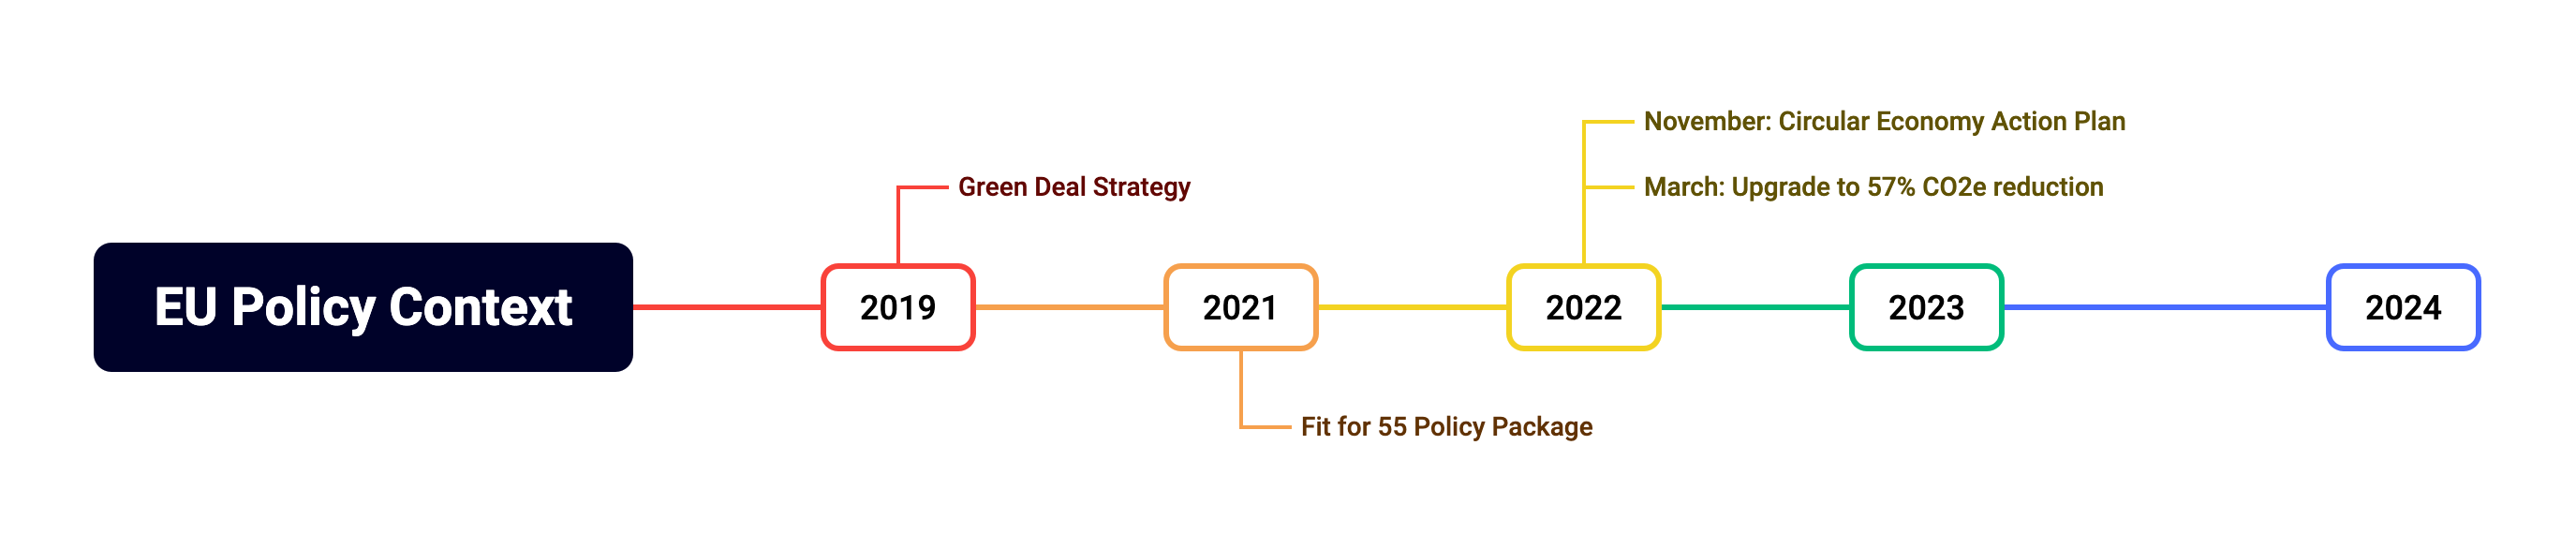
\includegraphics[width=1\linewidth,height=\textheight,keepaspectratio]{./images/sustainability/eu-policy-context.png}

}

\caption{EU Policy Context Timeline}

\end{figure}%

The above chart shows how the European Union has been on a path of
climate legislation transformation.

\begin{figure}

\centering{

\pandocbounded{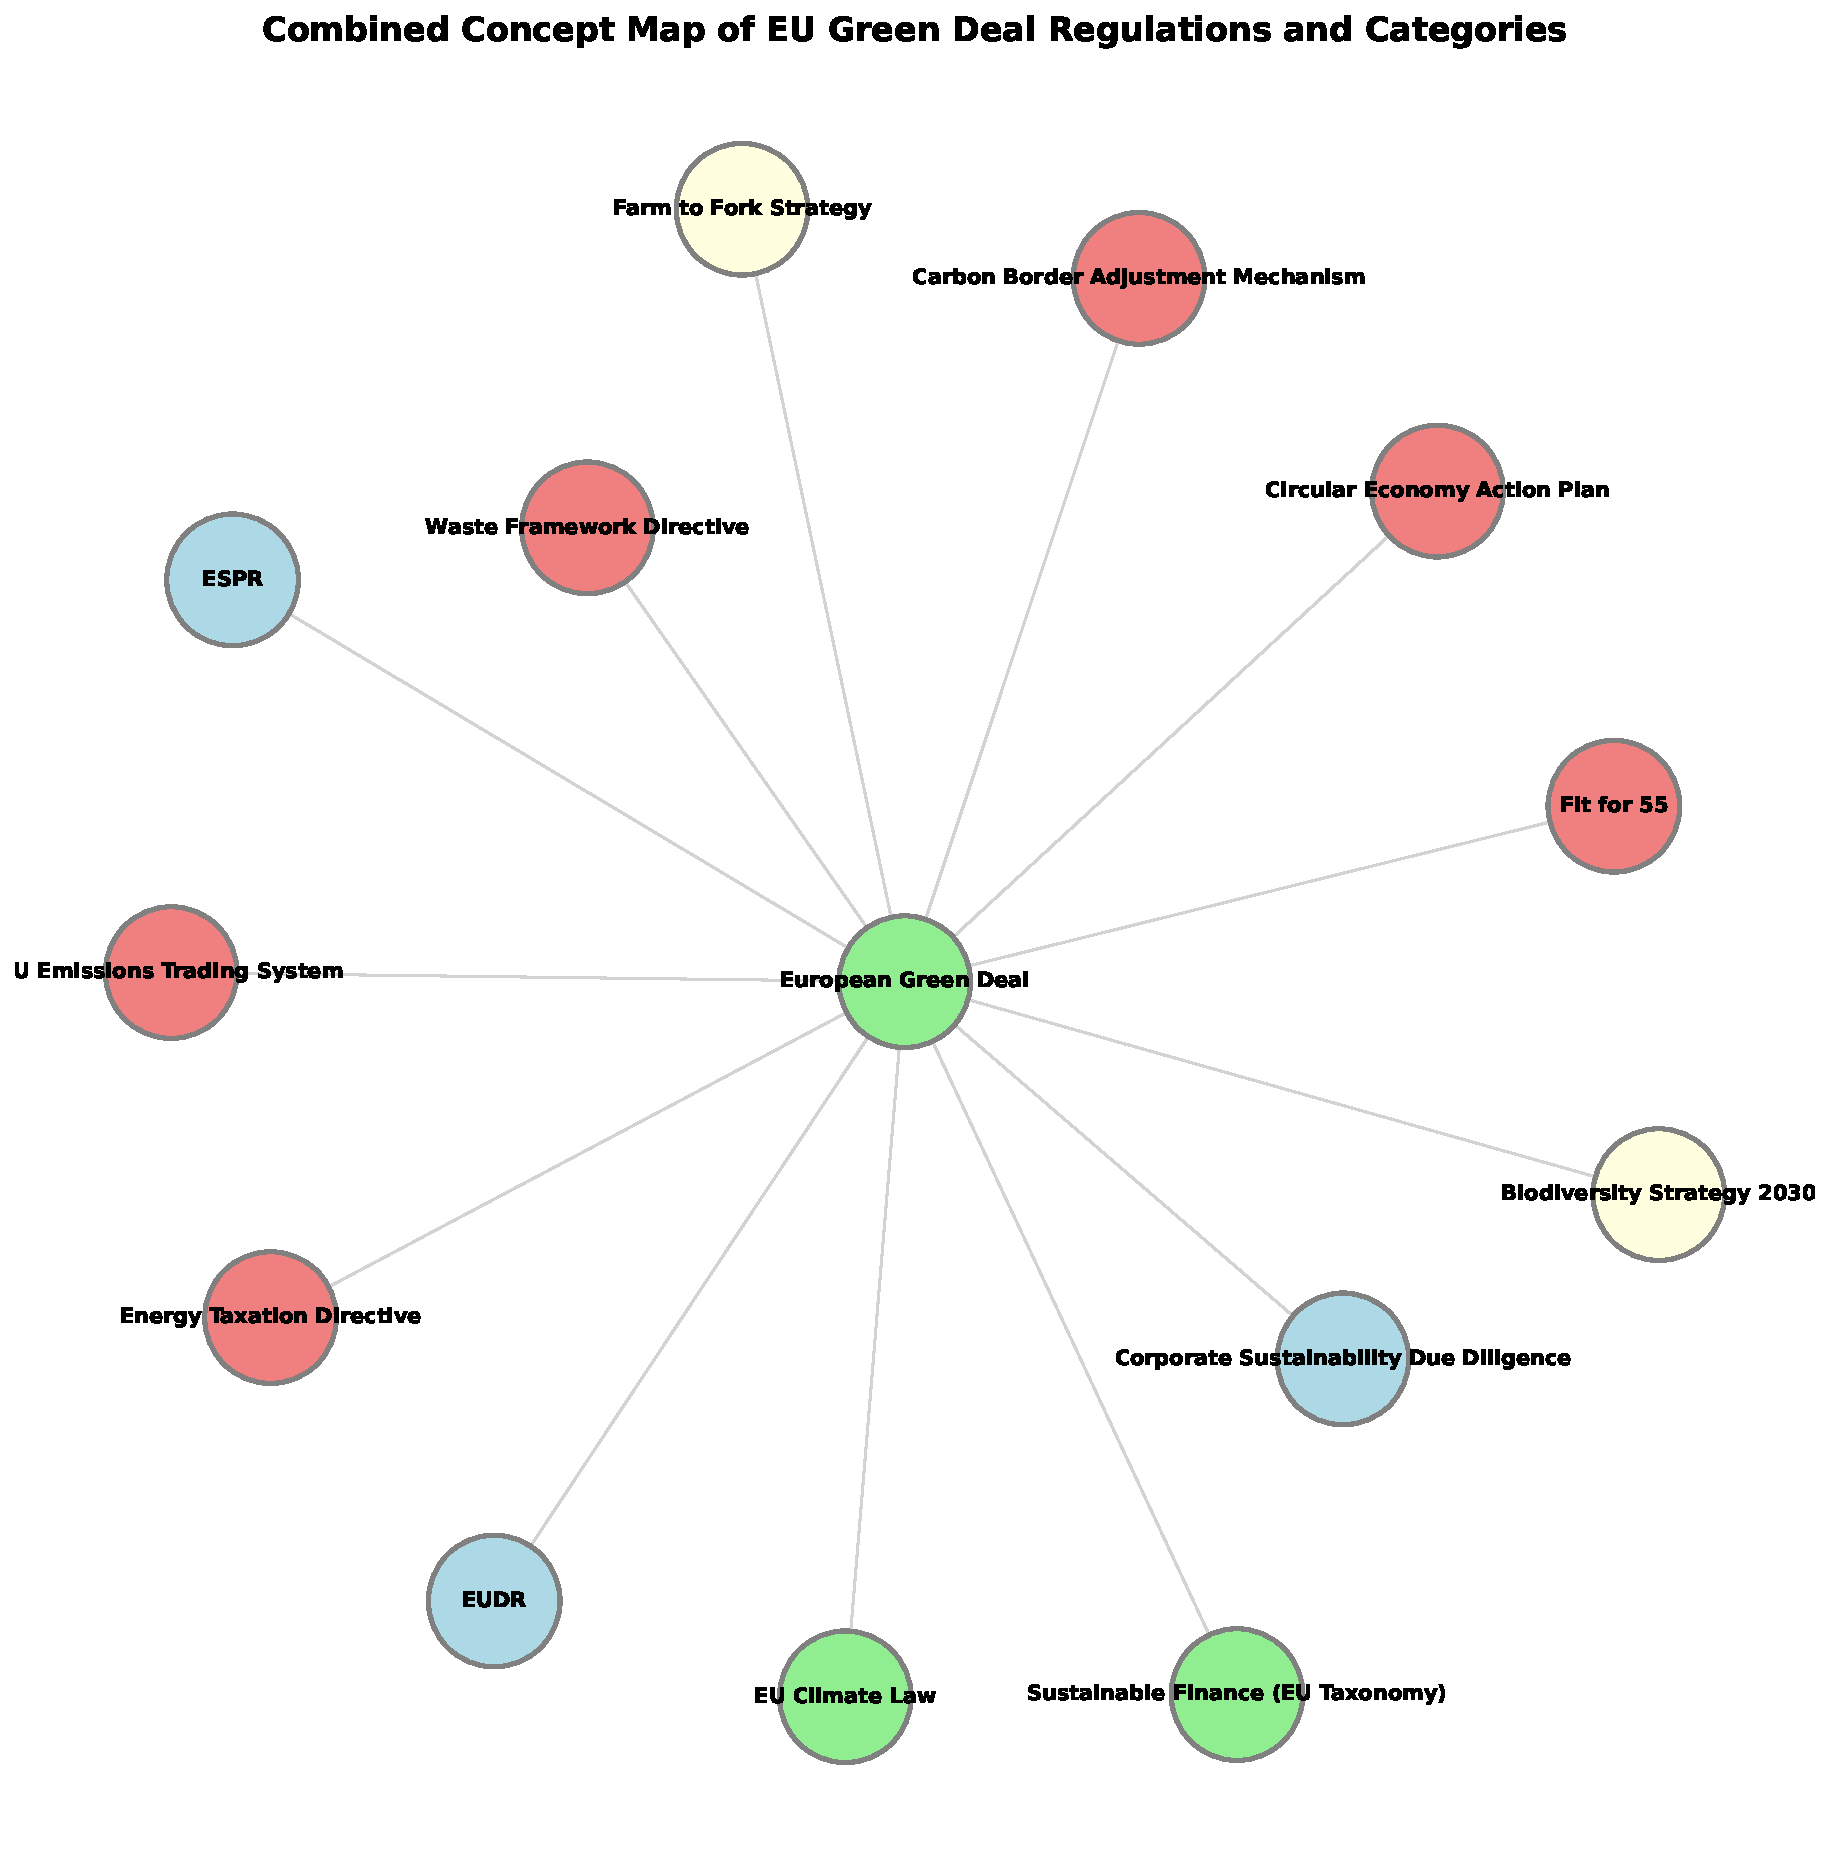
\includegraphics[keepaspectratio]{_thesis-nocite_files/figure-pdf/fig-eu-green-deal-output-1.pdf}}

}

\caption[The EU's Green Deal]{\label{fig-eu-green-deal}The EU's Green
Deal}

\end{figure}%

The above chart illustrates the European ``Green Deal''.

In the countries that make up the European Union (EU), a wide range of
legislative proposals, targets, organizations, and goals have existed
for decades. It's not that the EU didn't have an overarching
environmental policy before; rather it was vague and filled with
loop-holes. Upcoming laws cited above aim to harmonize approaches to
sustainability and raise standards for all members states, in turn
influencing producers who wish to sell in the EU common market. National
governments need to adapt EU legislation to local contexts. For example
Estonian government adopted the Estonian Green Deal Action Plan (Eesti
Rohepöörde Tegevusplaan) (Eesti Vabariigi Valitsus, 2022). From the
legislative perspective, NFRD (Non-Financial Reporting Directive) is
replaced by CSRD (Corporate Sustainability Reporting Directive) and ESRS
reporting is the standard to meet CSRD requirements.

The EU is also concerned with supply-chain deforestation. The ESPR
(Sustainable Products) and EUDR (European Union Deforestation
Regulation) work hand-in-hand as part of EU's legislative efforts to
promote sustainability. EUDR applies to all products placed on the
market from December 2024 and June 2025 for small businesses. Greenpeace
has called the EUDR \emph{``first step to end its complicity in the
reckless destruction of these life-support systems''} - yet to become a
success story, there needs to be follow through, integrating forest
protection throughout the economy. Some of the steps to achieve this
include the EU \emph{taxonomy of environmentally sustainable economic
activities} published by the Technical Expert Group (TEG) on sustainable
finance, as detailed in the report by (\emph{{EU} Taxonomy for
Sustainable Activities}, n.d.). The proposal for a Nature Restoration
Law by the European Commission requiring member countries to restore
20\% of EU's degraded ecosystems by 2030 and full restoration by 2050
has not yet passed (as of writing) (\emph{Scientists Urge {European
Parliament} to Vote for Nature Restoration Law}, 2023) and is facing a
backlash (David Pinto, 2023).

Certainly the EU is not the only region legislating to promote
sustainability; sustainability policy context is shifting around the
world. There are legislative efforts in numerous jurisdictions, which
have passed laws which aim to reduce the environmental impact of
products throughout their lifecycles. In the US, the \emph{Inflation
Reduction Act} provided funding to development of de-carbonizing
technologies and includes plans to combat air pollution, reduce green
house gases and address environmental injustices (Rajagopalan \&
Landrigan, 2023). In Australia, the Product Stewardship (PS) scheme also
includes an investment fund targeted at increasing the recycling rates
of specific products (Australian Government, 2024). Australia, Japan,
and Taiwan all have sustainable procurement schemes, prioritizing
greener products in public purchases (Australian Government Department
of Finance, 2025; Ministry of the Environment, Government of Japan,
2000; The Ministry of Environment of Taiwan, 2024).

I was torn whether to place \emph{politics} under \emph{sustainability}
or \emph{design}, and decided for the latter - as sustainability is
primarily \emph{descriptive}, using science to measure and present the
real situation, while design is \emph{prescriptive}: codifying decisions
about how do we live - in products and services. Design \emph{is}
political.

\subsubsection{Beyond Recycling: Default to Return, Repair,
Reuse}\label{beyond-recycling-default-to-return-repair-reuse}

(Gigerenzer, 2008) argues that heuristics - basically, rules of thumb -
can make more accurate predictions about the future than statistical
tools such as Bayesian and regression models, in certain contexts,
especially when data is incomplete or noisy. This aligns with Herbert
Simon's classic concept of bounded rationality, which suggests that
people make decisions not by fully optimizing, but by
\emph{satisficing}, i.e.~seeking good-enough options given limited time,
information, and cognitive capacity (Simon, 1955). (Gigerenzer, 2008;
Gigerenzer \& Selten, 2002) updated the concept to introduce the idea of
a toolbox of fast, dynamic, frugal heuristics - named ecological
rationality, showing how humans use only a small amount of information,
often ignoring most available data, adapting to specific environments:
heuristics aren't irrational; they work well because they exploit the
structure of real-world environments.

In the practice of design for sustainability, the recognizing that
humans use heuristics, translates to making strategic use of choice
architecture and \emph{the power of defaults}: displaying the most
sustainable option as the default - the oft-quoted example being green
power as the default choice on the German energy markets (Antonides \&
Welvaarts, 2020; Kaiser et al., 2020). Several research projects of
plant-based, vegan and vegetarian food defaults at (university) canteens
show 45-58\% increase in sustainable choices across studies (Boronowsky
et al., 2022; Erhard et al., 2023; Ginn \& Sparkman, 2024; A. W. Zhang
et al., 2024). (Simon Sterne, 2023) argues good UX is about helping the
user make decisions, which can be thought of as four key tactics: (1)
simplify complex choices, (2) intelligent defaults, (3) clear real-time
feedback on the outcome of each option, and (4) avoid unintended regret
by testing decision-support systems.

The universal recycling symbol creator Gary Anderson created the symbol
when he was an architecture student at USC (University of Southern
California) in 1970 at the age of 23, inspired by Silent Spring, Earth
Day, the Bauhaus, Bucky Fuller, Spaceship Earth, printing presses, and
the Woolmark logo for wool industry certification, and even the Mobius
strip, for a competition held by a packaging firm that was making paper
containers for packaging (Swap Society, 2023).

\subsubsection{Eco-Modulation: Extended Producer Responsibility
Incentive
Design}\label{eco-modulation-extended-producer-responsibility-incentive-design}

Eco-modulation is a legislative innovation, which makes harder to
recycle items more expensive for the producer. Recycling fees take into
account eco-design: an item from a single material is easier (cheaper)
to recycle than product from composite materials. Eco-modulation makes
the hidden cost of hard-to-recycle formats directly visible on the
invoice.

While Taiwan doesn't yet have a specific eco-design law, there are
various pieces of legislation promoting circular economy. Already in
1988, Taiwan implemented an Extended Producer Responsibility (EPR)
scheme, followed by a recycling system (initially focused on electronic
items) in 1998 (Chong et al., 2009). Eco-design initiatives in Taiwan
started at least as early as 1994, when Taiwanese companies and
universities noticed international sustainability trends and began to
implement their own sustainable design initiatives (Jahau Lewis Chen et
al., 2005).

The key to comparing Product Stewardship, Extended Producer
Responsibility (EPR), and Eco-Design is the scope, as illustrated in the
chart below. While Product Stewardship (PS) and Extended Producer
Responsibility (EPR) deal mostly with the end of the product life-cycle
(they are \emph{reactive}), including their disposal and recycling (EPR
going a step further than PS by shifting the responsibility to the
producer), eco-design moves sustainability up the design chain (being
\emph{proactive}), setting standards for making better products - in
essence, attempting to \emph{design-out} the waste.

\begin{figure}

\centering{

\pandocbounded{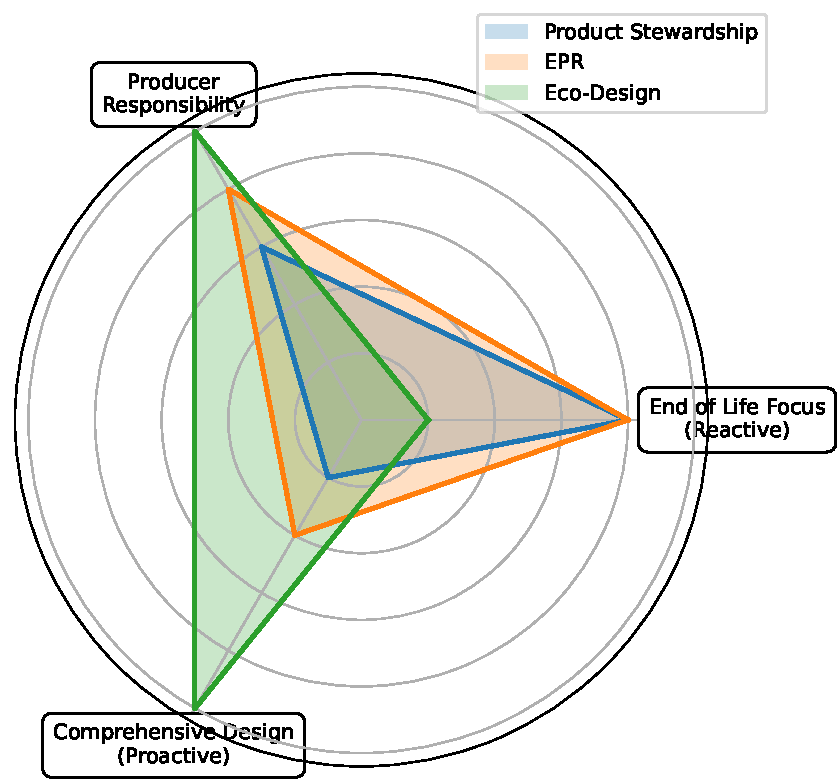
\includegraphics[keepaspectratio]{_thesis-nocite_files/figure-pdf/fig-ps-epr-output-1.pdf}}

}

\caption[Extended Producer Responsibility vs Product Stewardship vs
Eco-Design]{\label{fig-ps-epr}Extended Producer Responsibility vs
Product Stewardship vs Eco-Design}

\end{figure}%

Popular blogs such as (Kohli, 2019) and (Lose, 2023) offer many
suggestions how designers can help people become more sustainable in
their daily lives yet focusing on the end-user neglects the producers'
responsibility - termed Extended Producer Responsibility or ERP in waste
management studies.

Extended Producer Responsibility (EPR) is a policy tool first proposed
by Thomas Lindhqvist in Sweden in 1990 and described in detail in his
PhD thesis (Lindhqvist, 2000; Lindhqvist \& Lidgren, 1990), aimed to
encourage producers take responsibility for the entire life-cycle of
their products, thus leading to more eco-friendly products. In essence,
Extended Producer Responsibility enables companies to be responsible for
the entire life-cycle of the product. In California, part of the EPR
regulation is a large pool of funding for cleaning up historic pollution
resulting from industry Moolman (2024).

Nonetheless, EPR schemes do not guarantee circularity and may instead be
designed around fees to finance waste management in linear economy
models (Christiansen et al., 2021). The French EPR scheme was upgraded
in 2020 to become more circular (Jacques Vernier, 2021). In July 2024,
Latvia was the 4th EU country to join an textile-EPR scheme (\emph{New
{EPR} Requirements for Textiles in {Latvia} from {July} 2024 on}, 2024).
Strong consumer protection legislation (such as EPR) has a direct
influence on producers' actions. For example, in (HKTDC Research, 2022),
the Hong Kong Trade Development Council notified textile producers in
July 2022 reminding factories to produce to French standards in order to
be able enter the EU market.

In Europe, there's large variance between member states when in comes to
textile recycling: while Estonia and France are the only EU countries
where separate collection of textiles is required by law, in Estonia
100\% of the textiles were burned in an incinerator (as of 2018) while
in France textiles are covered by an Extended Producer Responsibility
(EPR) scheme leading to higher recovery and recycling rates (European
Commission. Joint Research Centre., 2021; Nordic Council of Ministers,
2020). Yet, some countries like Germany (75\%), Netherlands (45 \%), and
Denmark (43\%), which have no specific EPR scheme for textiles, report
higher collection rates than France, which with EPR collected only 38\%
of the textiles, however recovered 95\% of that through reuse and
recycling (Eurostat, 2022; \emph{Towards 2025 - Separate Collection and
Treatment of Textiles in Six {EU} Countries}, 2020).

The success of EPR can vary per type of product. For car tires, the EPR
scheme in the Netherlands claims a 100\% recovery rate
(Campbell-Johnston et al., 2020). (J. Peng et al., 2023) finds that the
\emph{Carbon Disclosure Project} has been a crucial tool to empower
Chinese auto-producers to adopt ERP schemes. Technological advancements
play a big role in recycling rates, as even badly sorted materials can
increasingly be recovered using AI; one example being Greyparrot AI,
which notes that even in the most advanced countries, 40\% of waste
sorting is still manual, opening an opportunity for automation (Natasha
Lomas, 2024).

While recycling rates are improving, (Steenmans \& Ulfbeck, 2023) argues
for the need to engage companies through legislation and shift from
waste-centered laws to \emph{product design regulations}. In the same
vein, and in the spirit of EU's EPR regulations, (Ruiz-Pastor \& Mesa,
2023) proposes an integrated \emph{product repairability index} (PRI).
(Lenovo, 08-29-22) suggests rethinking product design entirely to
inspire consumers expect more from the devices they buy. (Duriez et al.,
2022) shows how simply by reducing material weight of the product, it's
possible to design more sustainable transportation. However, the devil
is often in the details. (Formentini \& Ramanujan, 2023) study of Design
for Circular Disassembly (DfCD), introduces a Disassembly Effort Index
(DEI) to measure the disassembly time in seconds; their case study of
the End-of-Life (EoL) of an electrical kettle showed ignoring realistic
EoL failures (such as rusted screws), can lead to inaccurate
recommendations for circular design parameters.

Packaging is a rapidly growing industry, expanding on the back of online
shopping, which generates large amounts of waste materials, which, if
not reused or recycled, easily becomes garbage. Over 161 million tonnes
of plastic packaging is produced every year (Bradley \& Corsini, 2023).
Already more than a decade ago, (\emph{Detail-Rich Sustainable Packaging
{Product Database} Is an Industry First}, 2010)proposed a database of
green packaging to compare hundreds of sustainable packaging materials
and guide designers through environmental, performance, and cost
trade-offs in one unified tool, in order to help producers choose better
packaging - yet the problem is far from solved. More recently, (Bradley
\& Corsini, 2023) developed an analytical framework of key
sustainability factors, from an overview of 107 studies on reusable
packaging, finding customer acceptance, high return rates, supply-chain
shortening, and system standardization, as the key factors critical to
unlocking reusable packaging solutions at scale. A survey by PMMI, the
Association for Packaging and Processing Technologies, among industry
professional, found legacy equipment, higher material costs, and supply
consistency as the top barriers to sustainable packaging; in turn, vital
enablers were clear vendor guidance, proven material and equipment
solutions, and customer demand (\emph{Challenges and {Opportunities} in
{Sustainable Packaging Today}}, 2022). In response to legacy equipment
issues, (\emph{Sulapac -- {Replacing} Plastic}, n.d.) a large producer
of packaging, has proposed a wood-based, microplastic-free composites to
serve as drop-in replacements for plastics; a material even compatible
with existing molding, extrusion, and thermoforming production lines,
while slashing cradle-to-gate CO\textsubscript{2} emissions and
preventing microplastic pollution.

In food packaging specifically, (Ada et al., 2023) identified distinct
challenges from consumer acceptance to material-supply mismatches,
collection logistics, and regulatory gaps, underscoring the multifaceted
barriers to circular food packaging. Over 85\% of companies in the
``protein industry'': meat, poultry, seafood, and alternative proteins
have some type of sustainability initiative (\emph{Protein {Brands} and
{Consumers Alike Focus} on {Sustainability}}, 2022). Yet, having
sustainability programs does not make a company sustainable, case in
point being Coca Cola in the beverage industry. (Lerner, 2019) describes
Coca-Cola's plastic pollution problem, based on leaked audio, detailing
how Coca-Cola was exposed for lobbying against container-deposit laws -
aka Deposit Return Schemes (DRS), - aiming to misrepresented recycling
as a complete solution; strategies that stalled effective legislation
and maintained a ``green'' facade despite obstructing real
sustainability progress.

The \emph{``Plastic Waste Makers Index''} report lists large
corporations which produce plastic waste globally and provides some
useful statistics: single-use plastic rose by 6 million tonnes from 2019
to 2021, while just 3 million tonnes of recycling capacity was planned
by 2027 (as of the report date, 2023); in total, single-use plastic
generated 450 million tonnes of CO\textsubscript{2}eq emissions per
year; up to 98\% of the single-use plastic was produced from virgin
petrochemicals, while 2\% was from recycled material; meanwhile in
Taiwan, the Far Eastern New Century company boosted recycled content
from 2\% to 11\% in 2021 and plans to double its recycling capacity
(Minderoo Foundation, 2023). (Yap et al., 2023) Singapore disposes of
900,000 tonnes of plastic waste each year, out of which only 4\% is
recycled. Single-use plastics make up 44-68\% of all waste mapped by
citizen scientists (Kiessling et al., 2023).

\subsubsection{Scenario-Building: The Worst Futures and Designs for
Quality of
Life}\label{scenario-building-the-worst-futures-and-designs-for-quality-of-life}

Scenario-building is a key tool for sustainability, because
sustainability is so complex. Sustainable design cannot always predict
certain outcomes - instead, it can make use of scenarios to prepare for
several possibilities. In sustainability, there are rarely good choices.
Rather it's a question of avoiding the worst choices. One existing tool,
which has been widely used, is the En-ROADS climate change solutions
simulator; governments, organizations and individuals around the world
have used it explore climate scenarios based on interactive changes and
visualizations (Climate Interactive, n.d., 2023; Creutzig \& Kapmeier,
2020; Czaika \& Selin, 2017). Likewise, (Rooney-Varga et al., 2019)
shows the effectiveness of \emph{The Climate Action Simulation} in
educating users about \emph{success scenarios}. \emph{Life Cycle
Assessment} and \emph{Environmental Impact Analysis} are another set of
useful tools to provide eco-design scenarios (de Otazu et al., 2022).

While traditional economic thinking is based on a conflict between
nature and development, some new holistic models find there is potential
for synergy between economic, social, political, cultural, and
environmental metrics. For example, (Kaklauskas et al., 2023)`s
multi-criteria analysis of 169 countries and 238 cities, finds 71\%
average correlation between Climate Change and Country Success (C3S) and
Quality of Life (C3QL) indicators. In a similar vein, (Rieger et al.,
2023) develops an integrated science of wellbeing, linking humans'
psychological, biological, societal and environmental domains to guide
research and public policy, based on interactions between domain
experts.

Wellbeing Economy Governments is an example of country-level
collaboration in sharing expertise on sustainable development, looking
to bring post growth strategies and policy frameworks to the mainstream.
The concept of a wellbeing economy focuses on human and ecological
wellbeing rather than material growth since 2018 and includes Finland,
Iceland, New Zealand, Scotland, Wales, and Canada as founding members of
the network (Fioramonti et al., 2022).

(Popkova et al., 2022) argues that SDGs need to discussed in their
totality and uses factor analysis to link SDGs to institutions and
digital technologies; findings include SDG 3 (Good Health and
Well-Being) and SDG 17 (Partnerships for the Goals) progress through
institutions in developed countries and are most impacted by digital
technologies and digital knowledge index, meanwhile SDG 16 (Peace,
Justice and Strong Institutions) makes the most headway in developing
countries, which are starting from a lower base. Likewise, the German
Institute of Development and Sustainability (IDOS) has built a tool to
connect SDGs and their 169 targets to NDCs (Nationally Determined
Contributions), looking for synergies for effective climate action plans
and sustainable development strategies, visualizing a clear skew which
SDGs receive the most climate‐related commitments - SDG 2 (Zero Hunger),
SDG 6 (Clean Water and Sanitation), SDG 7 (Affordable and Clean Energy);
meanwhile SDG 14 (Life Below Water), and the SDG 3 social goals
discussed above, SDG 4 (Quality Education) and SDG 5 (Gender Equality),
are the least addressed in climate plans (Dzebo et al., 2023).

Eco-Design is about improving processes and optimizing resources. While
the goal of reducing harm is shared, the specifics will depend on the
industry. (Van Doorsselaer, 2022) Defines eco-design as \emph{``design
for X''} in a circular economy, thinking through the life cycle of a
product, tools, materials, production, use, and end-of-life phases.

In wine-making, (Manzardo et al., 2021) presents an Italian winery case
study, where a redesigned Merlot red wine procedure reduced in
environmental impacts from fuel and pesticide use in vineyards; the
8-step procedure included calculating the product's environmental
footprint and following the ISO 14006 standard, titled
\emph{``Environmental management systems --- Guidelines for
incorporating ecodesign''}. Finding uses for by-products, can improve
sustainability even more. (Iñarra et al., 2022) designed a circular
scheme for brewery left-overs, producing feed ingredients for
aquaculture; in a further step, using life-cycle assessment (LCA) and
optimizing logistics, reduced the aquafeed's environmental footprint
also by 6\%.

In architecture and the built environment, (Munaro et al., 2022)
conducted a comprehensive review of eco-design 288 articles, identifying
\emph{Design for Adaptability} and \emph{Disassembly} as the most
inclusive strategies, coining a new term DfAD; a framework linking DfAD
with lifecycle assessment tools is a promising are for research to
support sustainable construction.

In pharmaceuticals, (Bassani et al., 2022) proposes an approach to
eco-design using life-cycle assessment: optimizing packaging types,
alternative materials, transport, and weight reduction. A follow-up
study from the same group in 2023 extended the eco-design to a full
cradle-to-grave assessment and evaluated end-of-life alternatives
(Bassani et al., 2024).

In the printing industry, (Miyoshi et al., 2022) takes the example of
ink toner bottles and applies Life Cycle Simulation to show in a case
study how standardized compatibility between older and newer systems can
save resources and results in sustainability savings, highlighting how
re-manufacturing is an important strategy in circularity for reducing
CO\textsubscript{2} emissions and life cycle costs.

While these examples underline the industry-specificity of eco-design,
some authors attempt to come up with mores holistic approaches. For
instance (Ruiz-Pastor et al., 2022) developed ``CN\_Con'', a metric for
conceptual design, trying to measure circularity and novelty in
conjunction, by analyzing product functions, durability, material
origins, and end-of-life, while at the same time supporting creative and
circular design solutions in early stages.

On an international level, looking at companies operating on the
European Single Market, (Arranz et al., 2022) conducted a large-scale
study using machine learning on firm survey data from 870 organizations
across diverse economic sectors, acquired from the 2015 EU Public
Consultation on the Circular Economy conducted by European Commission,
comparing coercive pressures (regulations, subsidies, grants), normative
pressures (industry standards, professional networks), and mimetic
pressures (competitive imitation), finding normative and mimetic
pressure only enhance sustainability, if coercive pressure already
exists - i.e.~regulations are a key point of leverage. In summary,
enacting laws which support sustainability can shift complex systems
with many parties towards a circular economy, and be enhanced by
additional voluntary forces. However, a comparative analysis of OECD
green growth indicators for the periods 2004--2005 and 2019 across EU
member states found that green transformation do not correlate directly
with development level - instead each country's unique socio-economic
context plays a role: governance quality and income distribution shape
the effectiveness of regulatory frameworks, suggesting that coercive
policies must be tailored to national circumstances in order to
reinforce circular-economy adoption at scale(Cheba et al., 2022).

\subsection{Thinking in Systems to Re-Design Industries or Provenance
and
Traceability}\label{thinking-in-systems-to-re-design-industries-or-provenance-and-traceability}

As of 2025, \emph{circular economy} is a tiny part of the world economy.
(Circle Economy, 2022) reported in 2022 only 8.6\% of world economy was
circular and \emph{100B tonnes of virgin materials} was sourced every
year. An early pioneering innovator, (Jackson, 1996) showed through
detailed case studies how \emph{preventive environmental management},
redesigning industrial production at the source can avert pollution,
laying the conceptual groundwork for today's circular-economy models.
Many companies are investing into transforming their processes.
\emph{``{[}T{]}ransition to a low carbon economy presents challenges and
potential economic benefits that are comparable to those of previous
industrial revolutions''} (Pearson \& Foxon, 2012).

Futurists and visionaries adept at naming things have already listed the
5th, 6th, and even the 7th industrial revolution, pointing at robotics,
quantum computing, nanotechnology, and more, looking at current trends
and building scenarios for 2050 to envisioning a world with convergence
of bio-based and mineral-based technologies, widespread sustainability,
and energy-abundance (Chourasia et al., 2022; Ruiz Estrada, 2024). If
indeed, we're in an industrial revolution, it's possible to re-design
entire industries, and that is exactly the expectation sustainability
sets on businesses. Across all industries, there's a call for more
transparency. Conversations about sustainability are too general and one
needs to look at the specific sustainability metrics at specific
industries to be able to design for meaningful interaction. There's
plentiful domain-specific research showing how varied industries can
develop eco-designed products.

I use the lens of \emph{sustainability} - a complex term - to look at
how design can contribute to eco-friendly products, advocating a diverse
set design methods as a toolbox, where one can pick a suitable tool to
match the problem. While AI allows us to look at a larger number of
design scenarios than previously feasible, there are many approaches to
design for sustainability, with varied design practices that may be
relevant at different times in the process. Designing for sustainability
is fundamentally a hopeful act, imbibed with the belief that a healthier
world is possible - because health and sustainability are intrinsically
connected. As this research is \emph{practice-oriented} (i.e., my goal
here is to find design approaches that could influence my prototype), I
will focus on some fields of design which I hope relevant, fruitful, or
contextual to my project.

\emph{Eco-Design}, \emph{Circular Design}, \emph{Design for Circularity,
Cradle-to-Cradle Design}, \emph{Green Design}, \emph{Regenerative
Design}, \emph{Climate-Responsive Design}, \emph{Life-Centered Design,
Design for Human Rights, Multispecies Design, Designing for Health} -
designing for sustainability has been called with many names in diverse
contexts of use, using a diversity of approaches, with subtle
differences of emphasis and nuance, with same general goal of being more
sustainable. While EU legislation chose \emph{Eco-Design} as the
overarching title, researchers and practitioners discuss all of the
above on a frequent basis. (Ceschin \& Gaziulusoy, 2016) gives a
comprehensive overview of the main themes of sustainable design and the
main contributions and limitations in the well--researched
\emph{``Evolution of design for sustainability: From product design to
design for system innovations and transitions''}.

\begin{figure}

\centering{

\pandocbounded{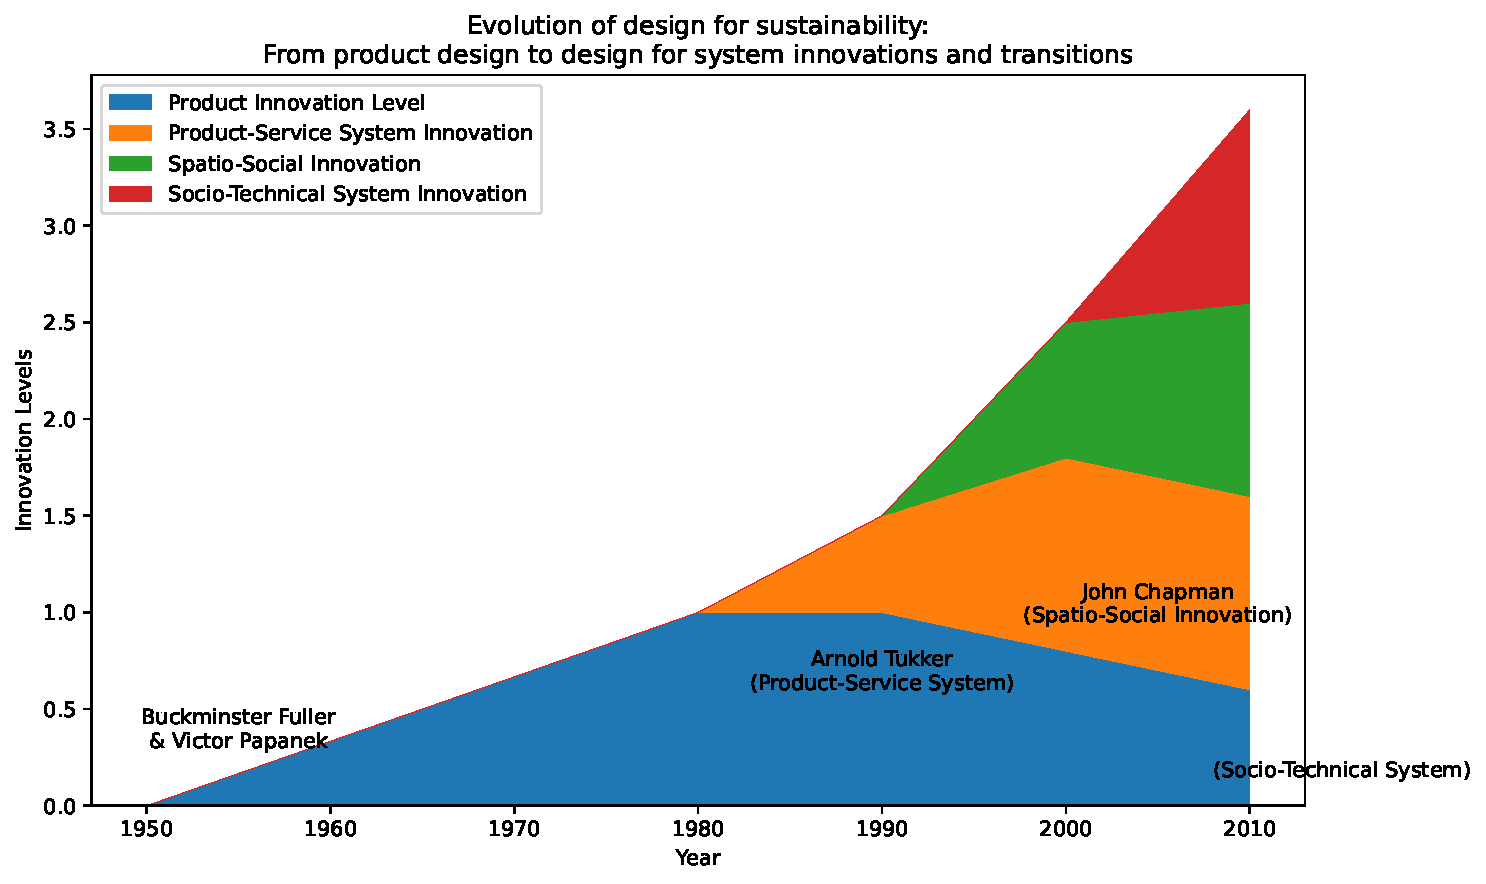
\includegraphics[keepaspectratio]{_thesis-nocite_files/figure-pdf/fig-dfs-history-output-1.pdf}}

}

\caption[History of Design for
Sustainability]{\label{fig-dfs-history}History of Design for
Sustainability}

\end{figure}%

\emph{Human-Centered Design} is the grandfather of design with
\emph{attitude}. There's even an ISO standard for human-centered design,
with the designated code ISO9241-210, revised as ISO 9241-210:2019
titled \emph{``Ergonomics of human-system interaction''} and up for
revision soon (ISO standards are reviewed every 5 years). Some of the
key takeaways include ``Understanding and specifying the context of
use'', ``Involving users throughout design and development'',
``Specifying user requirements'', ``Evaluating designs'',
``Multi-disciplinary Collaboration'', ``Iterative process'' and
``Continual Improvement'', and finally - usability is not enough, the
design should provide a user experience (UX) for human ``emotional
responses and satisfaction'' (ISO, 2019).

While \emph{Human-Centered Design} focuses exactly on what it says -
humans - \emph{Life-Centered Design} recognizes human impact on our
surrounding environment as well - making sure we include non-human
animals among our stakeholders. This is where we are getting on the
\emph{territory} of sustainability. While \emph{Human-Centered Design}
is ever popular, the effect humans are having on biodiversity is rarely
considered when designing. \emph{``{[}T{]}he design phase of a physical
product accounts for 80\% of its environmental impact''} notes(Borthwick
et al., 2022) in their framework for life-centered design. If we're
including \emph{other} lifeforms among our stakeholders, what can we
learn from them? \emph{Biomimicry} is about being inspired by nature
while \emph{Biodesign} focuses on design involving biology in the design
itself. Janine Benyus, who coined the word \emph{Biomimicry} (Benyus,
2009) looks at very practical cases of innovation where engineers and
biologist meet and (Dicks, 2023) provides a much more philosophical
account of following the example of nature. Focusing on the financial
sector, (Thomas \& Mantri, 2022)'s philosophical account advocates for
an ``inside-out'' design pattern, much like natural systems, starting
from the smallest structures to guarantee resilience and survival,
instead of trying to control their external environment. In a similar
vein, \emph{Material Ecology} is the wording preferred by the architect
Neri Oxman based at the MIT Media Lab working with biomaterials as a
proponent of \emph{Nature-Centric Design} that adheres to the principles
of ecological sustainability with both an ecologically conscious mindset
and practical toolset (Hencz, 2022). Language and our mental concepts
shape our reality, which makes language-creation an important tool for
sustainability. Neri Oxman's expressions in her (World Economic Forum,
2016) interview introduce some new vocabulary:
\emph{``ecology-indifferent''}, \emph{``naturing''}, \emph{``mother
naturing''}, \emph{``design is a practice of letting go of all that is
unnecessary''}, \emph{``nature should be our single client''}, which
reminds me how self-invented language gives an child-like freedom to
imagine new worlds.

\emph{Regenerative Design} suggests \emph{de}materializing (digitizing)
economies is not enough to be sustainable (by reduction of physical
impact). Design should look beyond reducing harm and find avenues to
\emph{regenerate} damaged or even completely destroyed natural systems
-- ecosystems, biodiversity, land, forests, lakes, rivers - natural
habitats.

\emph{Multi-Species Design} refers to the idea of considering non-human
life-forms as stakeholders of our design. (D. Metcalfe, 2015)`s PhD
Dissertation titled \emph{``The devastating effects that unsustainable
design practices have on the natural world and other species with whom
we share this planet''} gives a good overview of the work done is this
branch of design. In a similar vein, \emph{Biodiversity Inclusive Design
(BID)}, developed by (Hernandez-Santin et al., 2023) through a
systematic review of 14 design frameworks, presents a
\emph{'participatory ladder for non-humans'}; including core design
principles that position species' needs within urban planning to achieve
a biodiversity-positive multi-species environment. Multi-species design
and participatory design can work together. (Haldrup et al., 2022)
examines how participatory design can include non-human species as
co-creators of the urban commons; drawing on cases from Copenhagen,
Denmark and the Viskan River (in the textile town, Borås, Sweden), the
authors highlight sensory and aesthetic encounters, and attempts to
perceive the agency of non-human species in a collaborative design
processes (The University of Melbourne, Australia \& Roudavski, 2020).
Multi-Species Design has also entered the art-world thanks to (Marcus,
06-11-23) who uses artworks to think about how material design
strategies, surface textures, substrates, and bio-inspired composites,
can foster biodiversity and interspecies cohabitation in the built
environment. A very practical example helps one visualize this field the
best. (Kosová et al., 2023) introduces the BioGeo Ecotile, a
eco-engineering tile combining pits, holes, grooves, and crevices to
mimic natural rocky shores and provide multi-species
living-environments; deployed on rock armor and flood walls along
Edinburgh's coast in Scotland, Ecotiles supported significantly higher
intertidal species richness compared to smooth tiles, helping animals
make a life there. (Selvan et al., 2023) goes deep into data modeling
multi-variate calculations on how to build buildings, which support
ecology, coming up with a general framework for the architecture of
building envelopes, that resulted in 20\% higher local species richness
and up to 77\% higher abundance for individual species.

In most cases, designing for sustainability makes use of \emph{systems
thinking}, underlining the importance of looking at the entire
life-cycle of a product or service. (Rossi et al., 2022) shows how
introducing sustainability early in the design process and providing
scenarios where sustainability is a metric, it's possible to achieve
more eco-friendly designs. Yet, calculating what's sustainable is hugely
complex because decisions may have unforeseen ramifications. To take a
single example (Nuez et al., 2022) shows how electric vehicles may
increase CO\textsubscript{2} emissions in some areas, such as Canary
Islands, where electricity production is polluting. In sum, sustainable
design encompasses all human activities, making this pursuit an
over-arching challenge across all industries and all human activities
with the complex interdependence contained within these interactions.
(Engkvist, 2024) calls for \emph{Design Sociology}, design should take
account the product's effect on society, giving the example of highly
individualized understanding of individualized psychology and dopamine
cycles for creating social media, while disregarding the societal
effects, such as spread of misinformation. Lack of sustainability in the
design process is a \emph{bug} in the design approach.

\emph{Service Design}, (Ceschin \& Gaziulusoy, 2016) shows how design
for sustainability has expanded from a product focus to systems-thinking
focus placing the product inside a societal context of use. For example
(\emph{Cargo Bike {\textbar} {FREITAG}}, n.d.), recycled clothing maker
FREITAG offers sustainability-focused services such as cargo bikes so
you can transport your purchases and a network for \emph{shopping
without payment} = swapping your items with other members, as well as
repairs of their products. Loaning terminology from \emph{service
design}, the user journey within an app needs to consider each
touchpoint on the way to a state of success. \emph{Designing for Trust},
Weinschenk (2011) says \emph{``People expect most online interactions to
follow the same social rules as person-to-person interactions. It's a
shortcut that your brain uses to quickly evaluate trustworthiness.''}

\emph{Speculative Design} can also help us imagine
\emph{non-anthropocentric} (Edwards \& Pettersen, 2023; Hupkes \&
Hedman, 2022) as well as \emph{dystopian} futures (Pinto et al., 2021).
First introduced by (Dunne \& Raby, 2013) in their seminal book, the
field aims to question the intersection of \emph{user experience design}
and \emph{speculative fiction}. (Barendregt \& Vaage, 2021) explores the
potential of speculative design to stimulate public engagement; thought
experiments can spur public debate on an issue chosen by the designer.
Phil Balagtas, founder of The Design Futures Initiative at McKinsey,
discusses the value of building future scenarios at his talk at Google.
His favorite example, the Apple Knowledge Navigator, first appeared in
an Apple vision video in 1987 and took two decades to materialize in the
real world. It was inspired by a similar device first shown in a 1970s
episode of Star Trek as a \emph{magic device} (a term from participatory
design), which then inspired subsequent consumer product development. It
took another two decades, until the launch of the iPhone in 2007 - a
total of 40 years. Iteration has been the mainstay of software design,
incrementally improving the user experience, through a continuous
feedback loop; yet speculative design can help explore and imagine
possible futures by manifesting them in stories, artifacts, and
scenarios, empowering stakeholders to prepare for challenges and shape
policy, as well as ethical frameworks, beyond strictly product-centered
thinking (Google Design, 2019).

\emph{Participatory Design} and \emph{Speculative Design} can be
complementary as in the work of (Neuhoff et al., 2023), used together to
focus on engaging users deep in the design process to truly understand
their needs, contexts and interactions on a non-superficial level. For
both speculative and participatory design, the cost and makes it into a
niche activity. Generative AI holds the promise to allow designers to
dream up and prototype quicker. In order to build a future, it's
relevant to imagine and critique a future. By being quickly generate
prototypes, once can test out ideas with the future users involving more
of the community and stakeholders. To be able to build something, one
first needs to imagine it; imagination is crucial for change.
Speculative Design helps us envision future scenarios and be critical of
the current reality, by taking an alternative view-point. A related
field, \emph{Design Fiction}, goes even further by creating narratives
and artifacts that immerse participants in detailed visions of possible
futures, blending storytelling and tangible experiences. The
Massachusetts Institute of Technology (MIT) is a source of many
fantastic innovations, used to host The Design Fiction group (from
September 2013 to May 2018), which designed projects to
\emph{``stimulate discussion about the social, cultural, and ethical
implications of emerging technologies''}, coming up with design such as
a Brain-Controlled Interface for Spermatozoa, the Human Perfume,
capturing the smell of the people significant to the author, as well as
Pop Roach, for designing edible cockroaches (Design Fiction group, 2018;
A. Liu, 2017).

\emph{Climate-Responsive Design} embeds a building within the
environmental constraints of a place and looks for opportunities use the
land, wind, sun, local materials, and local vernacular history and
culture when considering a design. Architect Susanne Brorson suggests
sustainability should be considered in the earlier phases of design
instead of trying to fix problems later, discussing
\emph{climate-responsive design principles} (EVM maaarhitektuuri keskus,
2019). The sentiment is echoed by (S. Lee \& Doevendans, 2011) who
edited a volume on sustainable approaches of world-renowned architects:
\emph{``The principles of sustainable design are rooted in the
building's relationship to the site and its environmental conditions
such as topography, vegetation, and climate.''} The pioneering book
\emph{Architecture of the Well-Tempered Environment} laid out ideas for
integrating environmental concerns as part of architecture already in
the 1980s (Banham, 1999).

\emph{Cradle-to-Cradle Design} uses systems thinking focusing on the
reuse, re-manufacturing, and finally - recyclability - of products. The
Taiwanese Design Research Institute (TDRI) hosted a Nordic Circular
Design Forum in Taipei, where Scandinavian circular design practitioners
shared projects from several industries, highlighting how design
requires building relationships; it's not feasible to create a
sustainable product by oneself, as it takes a whole ecosystem (TDRI,
2021; \emph{台灣設計研究院({TDRI} ) on {Instagram}}, 2021).
\emph{Durability} is an important dimension for sustainability. High
quality durable products are more sustainable as they last longer and
less likely to be thrown away. Forming an emotional bond with the
product makes it feel more valuable (Zonneveld \& Biggemann, 2014).
(Chapman, 2009) argues in his seminal paper (and later in his book) for
\emph{``Emotionally Durable Design''}, the simple idea that we hold to
things we value and thus they are sustainable. We don't throw away a
necklace gifted to us by mom, indeed this object might be passed down
for centuries. (Rose, 2015) has a similar idea, where \emph{``Enchanted
Objects''} become so interlinked with us, we're unlikely to throw them
away. This has implications for sustainability as the object is less
likely to be thrown away.

As the above shows, there are many partially overlapping design words
created by different people for diverse purposes. Design vocabulary may
be created for distinguishing a particular type of design from another -
or to market oneself as the creator of the word. There are designers who
define / brand themselves by their design method. Design Studies, a
field that studies \emph{design} as a subject.

\subsection{Student Essentials: Consumer Goods, Clothes and
Food}\label{student-essentials-consumer-goods-clothes-and-food}

Food, clothes, and consumer goods (I'm omitting housing and transport
here) are part of the immediate environmental impact of college
students. I will here focus on 3 industries that are relevant for
college students.

\subsubsection{Fast-Moving Consumer
Goods}\label{fast-moving-consumer-goods}

Fast-Moving Consumer Goods (FMCG) also known as Consumer Packaged Goods
(CPG) are large global conglomerates operating with low margins and high
volumes (Toh, 2024). The largest of them have several billions in
revenue (Kenton, 2024). Rise of e-commerce has pushed logistics
companies to increase delivery efficiency to keep up with FMCG sales
(Deliverect, 2024).

\begin{figure}

\centering{

\pandocbounded{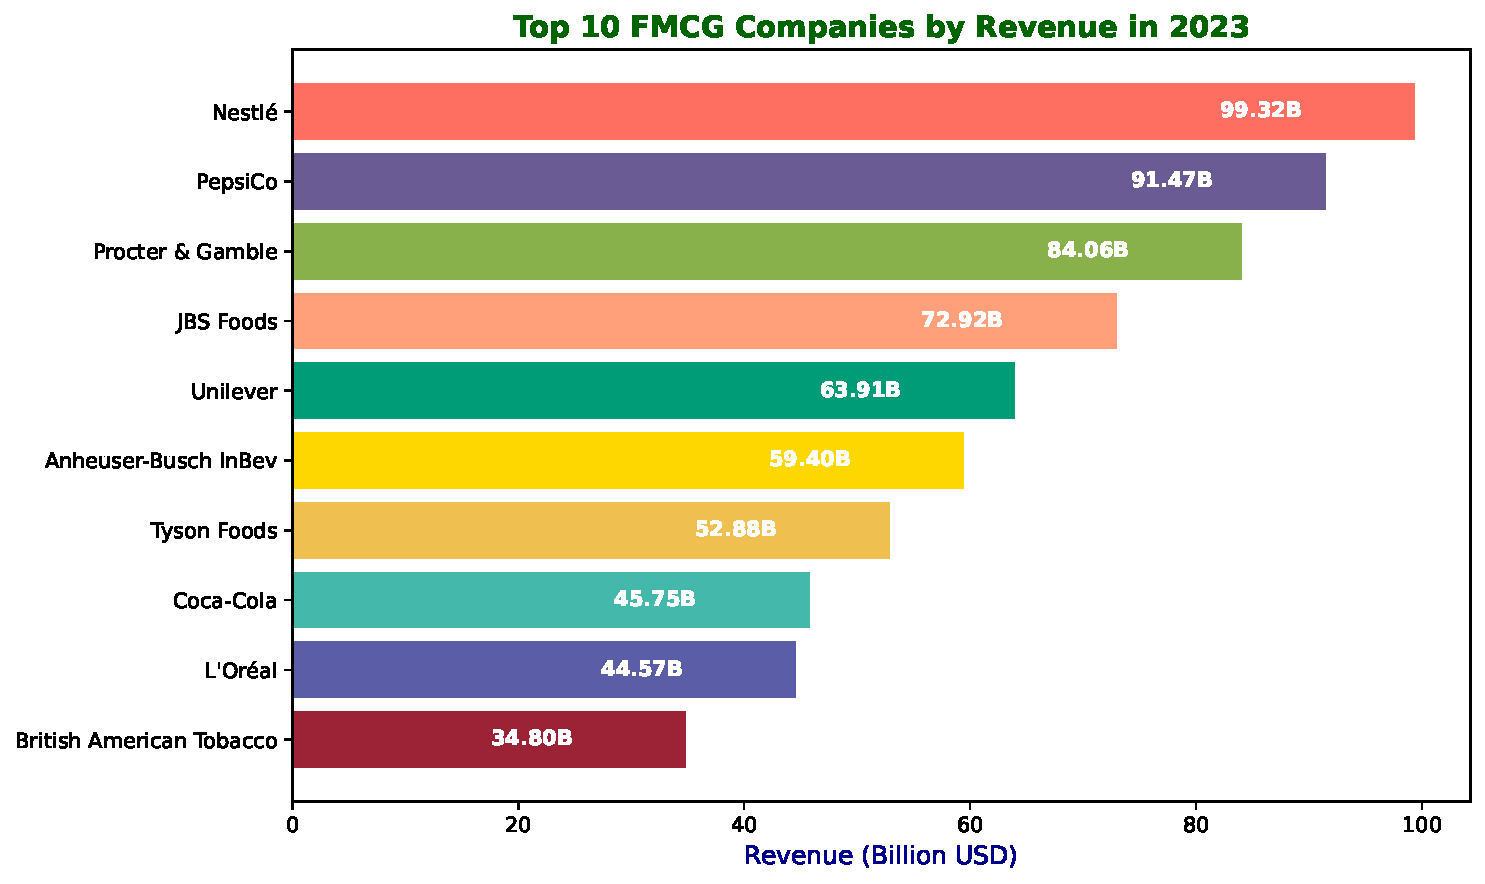
\includegraphics[keepaspectratio]{_thesis-nocite_files/figure-pdf/fig-consumer-goods-output-1.pdf}}

}

\caption[Consumer Goods]{\label{fig-consumer-goods}Consumer Goods}

\end{figure}%

In China, while there are signs of young Chinese consumers valuing
experiences over possessions, the raw sales growth numbers show
consumerism is only increasing (Claudio-Quiroga et al., 2025; Hui et
al., 2025; Y. Jiang, 2023; X. Zhang, 2025).

\subsubsection{Clothes and the (Fast) Fashion
Industry}\label{clothes-and-the-fast-fashion-industry}

Just like Fast-Moving Consumer Goods, fast fashion operates with low
margins and follows consumer trends. Young people are the largest
consumers of fast fashion (\emph{Young {Consumers}' ({Complicated})
{Love For Fast Fashion In} 3 {Stats}}, n.d.). (In European Environment
Agency, 2022 European Environment Agency (EEA)) estimates based on trade
and production data that EU27 citizens consumed an average 15kg of
textile products per person per year. (Textile Exchange, 2021) Fashion
industry revenue is above USD 1.5 trillion; COP26 policy calls for 45\%
cut in emissions by 2030. The European Commission wants to reduce the
impact of fast fashion on EU market (ERR, 2022). There are other local
policy initiatives aiming to tackle the waste problem. For example the
New Standard Institute's proposed \emph{``Fashion Act''} to require
brands doing business in New York City to disclose sustainability data
and set waste reduction targets (Emily Chan, 2022b). In California, the
\emph{Garment Worker Protection Act} covers 45000 garment workers with
wage and safety safeguards (\emph{Lily {\textbar} Mindful + Active
Living on {Instagram}}, n.d.).

In terms of total figures, the 2.4 Trillion USD fashion industry
contributes 2\%-8\% of total global green house gas (GHG emissions);
100B USD is lost to lack of recycling; contributes 9\% of microplastics
(Adamkiewicz et al., 2022). (\emph{New {Standard Institute}}, n.d.)
similarly estimates the apparel \& footwear account for \textgreater{} 8
\% of global GHG and could rise up to 60\% by 2030.\\
(Centobelli et al., 2022) reports fashion industry year uses 9B cubic
meters of water, 1.7B tonnes of CO\textsubscript{2}, 92 million tonnes
of textile waste. (Emily Chan, 2022c) as things stand now, fashion
companies can't be held accountable for their actions (or indeed, their
lack of action), driving calls for extended producer responsibility.
(Köhler et al., 2021) Globally 87\% of textile products are burned or
landfilled after 1st consumer use. (Millward-Hopkins et al., 2023) shows
how 50\% of the textile waste in the UK is exported to other countries,
often to be dumped as trash in landfills or burned. (Tian Macleod Ji,
2024) found fast fashion propels 26 million tons of clothing in China's
landfills annually. In Ghana, research across several dumpsites revealed
up to 12\% of the landfill consisted of textile waste (Gyabaah et al.,
2023). The (\emph{Clean {Clothes Campaign}}, n.d.) decries how
\emph{``{[}t{]}he mainstream fashion industry is built upon the
exploitation of labor, natural resources and the knowledge of
historically marginalized peoples''}; in 2018, 3/5 of the 100 billion
garments produced globally ended up in landfill within one year of sale.
(FashionChecker, 2023) reports none of the top global apparel brands
pays a living wage; 60\% of garment workers are women earning below-men
wages. Yet, for certain countries this production is crucial; the
Bangladesh Garment Manufacturers and Exporters Association reports 24\%
annual growth in global market and makes up a whopping 81\% of the
exports of the country (\emph{{BGMEA} {\textbar} {Home}}, n.d.; Daily
Sun, 2022).

It's hard to make improvements to a system in an opaque environment.
(Emily Chan, 2022a) writes there's not enough transparency in the
fashion industry - greenwashing is prevalent - and introduces Fashion
Revolution's Fashion Transparency Index, in order to tackle the very
issues mentioned above (Fashion Revolution Foundation, 2022). Similarly,
(Wikirate, 2022b) presents itself thus: \emph{``Among the Index's main
goals are to help different stakeholders to better understand what data
and information is being disclosed by the world's largest fashion brands
and retailers, raise public awareness, educate citizens about the social
and environmental challenges facing the global fashion industry and
support people's activism''}. Already in 2018, Sourcemap launched the
\emph{``Open Apparel Registry''}, a crowdsourced digital map of apparel
factories, creating a standardized database of factory names and
addresses to enhance supply-chain transparency (Mowbray, 2018).
Sustainable fashion company evaluations platform Good On You rated 5821
brands in 2023; yet most large labels with climate targets publish no
progress data (Good On You, 2023). The Fossil-Free Fashion Scorecard
graded 43 brands; 15 scored ``F'' and the sector average was a ``D''
(Stand.earth, 2023). Making use of these indexes, YouTuber
(imperfectidealist, 2020) proposes a 7-step checklist to help consumers
spot greenwashing, focused on transparency, such as if the producer has
published a full list of suppliers. While consumer understanding of
sustainability is growing, it's not necessarily very specific; for
example (Mabuza et al., 2023) shows consumer knowledge of the effects of
apparel coloration is very limited.

Nonetheless, change is happening. Qima, a company which provides
inspection and certification services for the fashion industry, found
that in 2023 inspection demand for products coming from China rose 5.4\%
year-on-year, specifically 13\% from the US, 27\% from Germany, 32\%
from the UK, and 69 \% from Mexico, demonstrating the global nature of
the business, while \emph{near-shoring} and \emph{re-shoring} accounted
for 10\% of the U.S. and EU-based buyers' procurement, underscoring the
growing need for supply chain visibility and adaptability (QIMA, 2024).
One example of a blockchain-based fibre-to-garment traceability
solution, live with 100+ brands, is (\emph{Textile {Genesis}}, n.d.);
other blockchain-based approaches are discussed at length in a dedicated
section.

There's a growing know-how on how to design sustainable fashion and
which materials to use; for instance the \emph{``Handbook of Footwear
Design and Manufacture''} includes a special chapter on green design
specifically for shoes (Leung \& Luximon, 2021). The \emph{``Circular
Design HOW''} toolkit launched 2021 to guide Baltic designers in
cradle-to-cradle approaches for circular textiles (Eesti Disainikeskus I
Estonian Design Centre, 2021). Estonian Academy of Arts' sustainable
fashion open course reached 9 European universities in 2022, covering
eco-materials and ethical sourcing (Eesti Kunstiakadeemia, 2022). And
certainly there are many more examples globally.

However, for ethical fashion practices to reach scale, materials do
matter a lot. (Textile Exchange, 2023) reports global fiber output
reached 116 million tonnes in 2022; polyester alone was 54\% percent of
the total. Access to better materials is crucial and industry
collaboration can raise the bar for everyone, such as the Better Cotton
Initiative (Better Cotton, 2023). One example of an ethical brand is
(\emph{Sheep {Inc}. - {Softcore Radicals}}, 2023), which promises to
sequester 14kg of CO\textsubscript{2}eq per kg of wool (footprint per
finished sweater is 0.04 kg CO\textsubscript{2}eq), by using wool from
Merino sheep with regenerative practices. Robert Gentz, the Co-CEO and
co-founder of Zalando, a large European online retailer, says fast
fashion must disappear within the next decade (citing 40\% of wardrobes
are never worn), launching a separate brand called Zign, built around
sustainable materials and ethical production practices, with at least
20\% recycled content and 50\% eco-friendly materials per item
(Remington, 2020; Storbeck, 2021). Improved technology for recycling is
in the pipeline; for example (Infinited Fiber, 2023; Karila, 2024)
produces a premium fiber called Infinna, using its pulp-to-fibre
recycling tech, from waster materials - and is being used by sustainable
brands such as Patagonia.

The story of Patagonia has inspired many to see that a financially
successful, eco-friendly fashion business is a possibility; yet
Patagonia's 1 \% for the Planet pledge that has delivered about USD 140
million to grassroots environmental groups since 1985, seems like a drop
in the bucket compare to the scale of the problem (Chouinard, 2005). The
``Generation Rewear'' documentary documents the strides newer
sustainable fashion brands are making; yet a survey made for the film
showed 64\% of UK consumers wear items only once, leading to 350000
Tonnes of clothing landfilled yearly (Vanish UK, 2021).

Digital Product Passports will be mandatory for fashion under EU
Eco-design and EPR rules between 2026 and 2030, enabling ethical
shopping (\emph{Transparency and Sustainability Platform - {Renoon}},
2023). New apps make alterations and repairs made easy: SOJO
door-to-Door service raised USD 2.4 million pre-seed funding for a
clothes repairs service, cutting waste and emissions (\emph{{SOJO} -
Door-to-Door Clothing Alterations and Repairs}, 2023).

\subsubsection{The (Fast) Food Industry}\label{the-fast-food-industry}

Food production is a large greenhouse gas emitter. Global warming causes
droughts and extreme weather, wars and conflicts, which in turn
increases the volatility in food prices (Eshe Nelson et al., 2023).
(Nabipour Afrouzi et al., 2023) reports the agricultural sector
contributes approximately 25\% of the total CO\textsubscript{2}
emissions and 13.5\% of the total global anthropogenic greenhouse gas
emissions. (Poore \& Nemecek, 2018) suggests a slightly higher 26\% of
carbon emissions come from food production. (Saner et al., 2015) reports
dairy (46\%), meat and fish (29\%) products making up the largest GHG
emission potential. Livestock products (meat) are 15\% of agricultural
foods valued at €152 billion in 2018 globally (A. S. Patel et al.,
2023). (J. L. Bailey \& Eggereide, 2020) shows how the Norwegian
government plans to increase salmon production 5x by 2050; the demand
for food is increasing.

Re-designing the industrial food systems for an increasing global
population is a challenge - yet improvements are possible at every step
of the way. For example, an Italian retail supermarkets worried about
their carbon footprint ran a pilot program, which cut food + packaging
waste emissions from 436 kg CO\textsubscript{2}eq to 339 kg
CO\textsubscript{2}eq per store per year (total 22\% emissions
reduction) (Marrucci et al., 2020). Perennial (multi-year) crops are
less carbon intensive, reducing inputs of gasoline, labor, etc. (Aubrey
Streit Krug \& Yin Lu, 2023), yet large agritech companies like Monsanto
rely on selling seeds annually for profits putting them at odds with
perennial crops; single-year seeds have led to farmer suicides when
crops fail in poor communities.

Supply chain innovation in food industries may enable more transparency.
Provenance and traceability of food has implications for sustainability
and health. Food fraud is a contentious issue which requires new
science- and legislation-based solutions. One example is \emph{fake
honey}, meaning synthetic honey, or actual honey fraudulently blended
with cheaper sugar syrup, which can pass some laboratory tests,
requiring improved technology, such as DNA-analysis to find real honey
(ERR, 2023; X. Song et al., 2020). China is the world's largest honey
producer, making about 24\% of world total (Food and Agriculture
Organization of the United Nations, 2023) and has been implicated in
tampering with their product. Apimondia, the International Federation of
Beekeepers' Associations, canceled its annual honey award because of
wide-spread supply-chain fraud, as they were unable to guarantee the
authenticity of honey (Ungoed-Thomas, 2024). The same is true for cocoa
beans, which are at high risk from food fraud (E. Fanning et al., 2023).

Complex supply chains make seafood (marine Bivalvia, mollusks) logistics
especially prone to fraud, leading to financial losses and threats to
consumer health (Santos et al., 2023). (C.-H. Chang et al., 2021)
\emph{fish fraud} is a large global problem, but it's possible to use
DNA-tracking to prove where the fish came from. In Taiwan, the 27 KURA
SUSHI branches sold more than 46 million plates of sushi in 2019.
Illegal, unreported and unregulated fishing (IIU) fishing is widespread;
the EU is adopting countermeasures (D. E. Kim \& Lim, 2024).
Likewise,(Katie Gustafson, 2022) proposes a \emph{``Uniform traceability
system for the entire supply chain''} for seafood and (Mamede et al.,
2022) proposes fingerprinting of Sea Urchin for seafood tracing.

In total, the world consumes around 200 million tonnes of fish and
seafood every year, including wild catch and aquaculture (fish farming)
(Ritchie \& Roser, 2021). Precise and recent data about the fishing
industry is hard to come by. However, by some estimates, industrial
fishing accounts for approximately 75\% of the entire global catch, the
rest being artisanal fishing; 26\% of the catch is caught using bottom
trawling and dredges, which are highly damaging to the natural
environment; and 10-12\% using mid-water (pelagic) trawls, which are
somewhat less intrusive; around 20-30\% of the fish is caught using
large nets; around 6-7\% using industrial longlines (both surface level
and deep-set); and the rest is caught using a variety of other fishing
gear (Amoroso et al., 2018; Cashion et al., 2018; Hilborn et al., 2023;
Jacquet \& Pauly, 2022). About 10.8 \% of total catch is discarded;
bottom-trawling alone accounts for 46\% of discards (Pérez Roda et al.,
2019). (Muñoz et al., 2023) calls for banning of bottom trawling. (Sala
et al., 2021) notes that only 2.7\% of the world ocean is highly
protected and calls for a globally coordinated effort to protect marine
biodiversity.

Given these statistics, (Springmann et al., 2021) proposes veganism is
the most effective decision to reduce personal CO\textsubscript{2}
emissions. The food sovereignty movement, born in the late 1990s,
champions everyone's right to healthy and sustainable food, focusing on
\emph{local food systems} to bring producers and consumers closer
together, planting seeds and growing food in the cities, countryside,
and even indoors (Stall-Paquet, 2021). In a similar vein, the \emph{Farm
to Fork} European Union policy proposes to \emph{shorten the supply
chain} (meaning less change for fraud and fewer emissions) from the
producer to the consumer and add transparency to the system (Financial
Times, 2022). In Japan, one startup in this space is ``Secai Marche'',
self-described as ``Asia's Food Supply Chain'', operating a cold chain
and fulfillment platform, connecting farmers across Japan and Southeast
Asia to more than 500 retailers, delivering over 4000 distinct products
(SKUs), including vegetables, fruits, eggs, seafood, across its
transparent system, with AI-based demand-forecasting and optimized
truck-routing (Catherine Shu, 2023).

However, a local Taiwanese study refutes the idea that local
\emph{``farm-to-fork''} sourcing is greener in terms of carbon footprint
and environmental impacts; taking a case-study of ice-cream production
in Taiwan, the authors find sourcing ingredients from local, small-scale
farming in Taiwan, is more carbon-intensive in comparison with
ingredients imported from large-scale industrial farms in New Zealand
and Sri Lanka, even if accounting for the higher transportation
emissions (Y.-C. Huang et al., 2025).

(Lulovicova \& Bouissou, 2023) apply a territorial life cycle approach
to evaluate local food policies in Mouans Sartoux, France, and
demonstrate that simply reducing food miles is not enough to ensure a
lower environmental footprint; the biggest drivers of total impact are
changes in farm practices, aggregation methods, retail infrastructures,
and procurement contracts, rather than proximity alone - local supply
chains can outperform global chains \emph{if} local food policies
combine geographic proximity with improvements in on-farm efficiency,
logistics, energy use, and local retail systems, to realize true
sustainability gains.

It comes down to \emph{what} is compared to \emph{what}.

A local Taiwanese vertical farm, ``Yes Health iFarm'' (largest indoor
vertical farm in Asia as of 2018), spans 15 stories and employs 130
staff; they use LED lighting tailored to specific plant type, growing 30
varieties of edible plants (e.g.~arugula, ice plant, mustard leaf,
etc.), with high quality and `distinctive crunch and flavor'; the yield
is 100 times larger than in traditional farming, while using only 1/10
of the water; the factory is extremely clean, with zero pesticide
residues, zero heavy metal contamination, zero parasites, zero e coli,
low nitrates, low bacteria - demonstrating a high-tech driven approach
can provide exceptional resource efficiency and quality (Renée
Salmonsen, 2018).

Even when problems with food are discovered, solutions might take years
to emerge. For example, IARC (International Agency for Research on
Cancer) warns aspartame (artificial sweetener found in many soft drinks)
could cause cancer, confirmed by 2 separate studies; yet the
international standards for aspartame have yet to be updated 2 years
later (J. Fu, 2024; Riboli et al., 2023; Rigby, 2023).

Food is also about cuisine and culture; foods become popular if we hear
stories and see cuisine around a particular crop (Aubrey Streit Krug \&
Yin Lu, 2023). Food is about enticing human imagination and taste buds.
That is to say, improving food systems is not only about technical
details. Culture, community, cuisine, and storytelling can all play a
part to have better quality food and reduce food waste. While perhaps
over-romanticizing mushrooming, Anna Lowenhaupt Tsing's ethnographic
exploration in her book about the matsutake mushroom illustrates how
foragers and distributors collaborate across damaged ecosystems to
sustain a cross-border commodity chain becoming a sign of ecological
resilience, where disturbed forests altered by logging and industrial
activities; mushrooms form a ``gift economy'' that connects rural
pickers in Oregon, Japan, China, and Finland with affluent urban
consumers around the world; the price is high due to the foraging nature
of the collection (some sources call it the most expensive mushroom in
the world, sold at over \$1000 USD per kg, no intensive farming
practices involved); the author believes this is a type of collaboration
that does not depend on endless economic growth (personally, I would
describe it as economics of luxury goods) - in any case, it does remind
us that cultural narratives and local know-how (e.g.~cultural products)
do influence food and \emph{perhaps} can play a small part in more
resilient and sustainable food systems (Remley, 2025; Tsing, 2015; X.
Yang et al., 2008).

Coming back to apps, there are several initiatives aimed at reducing
food waste by helping people consume food that would otherwise be thrown
away, including Olio and Too Good To Go.

\begin{figure}[H]

{\centering 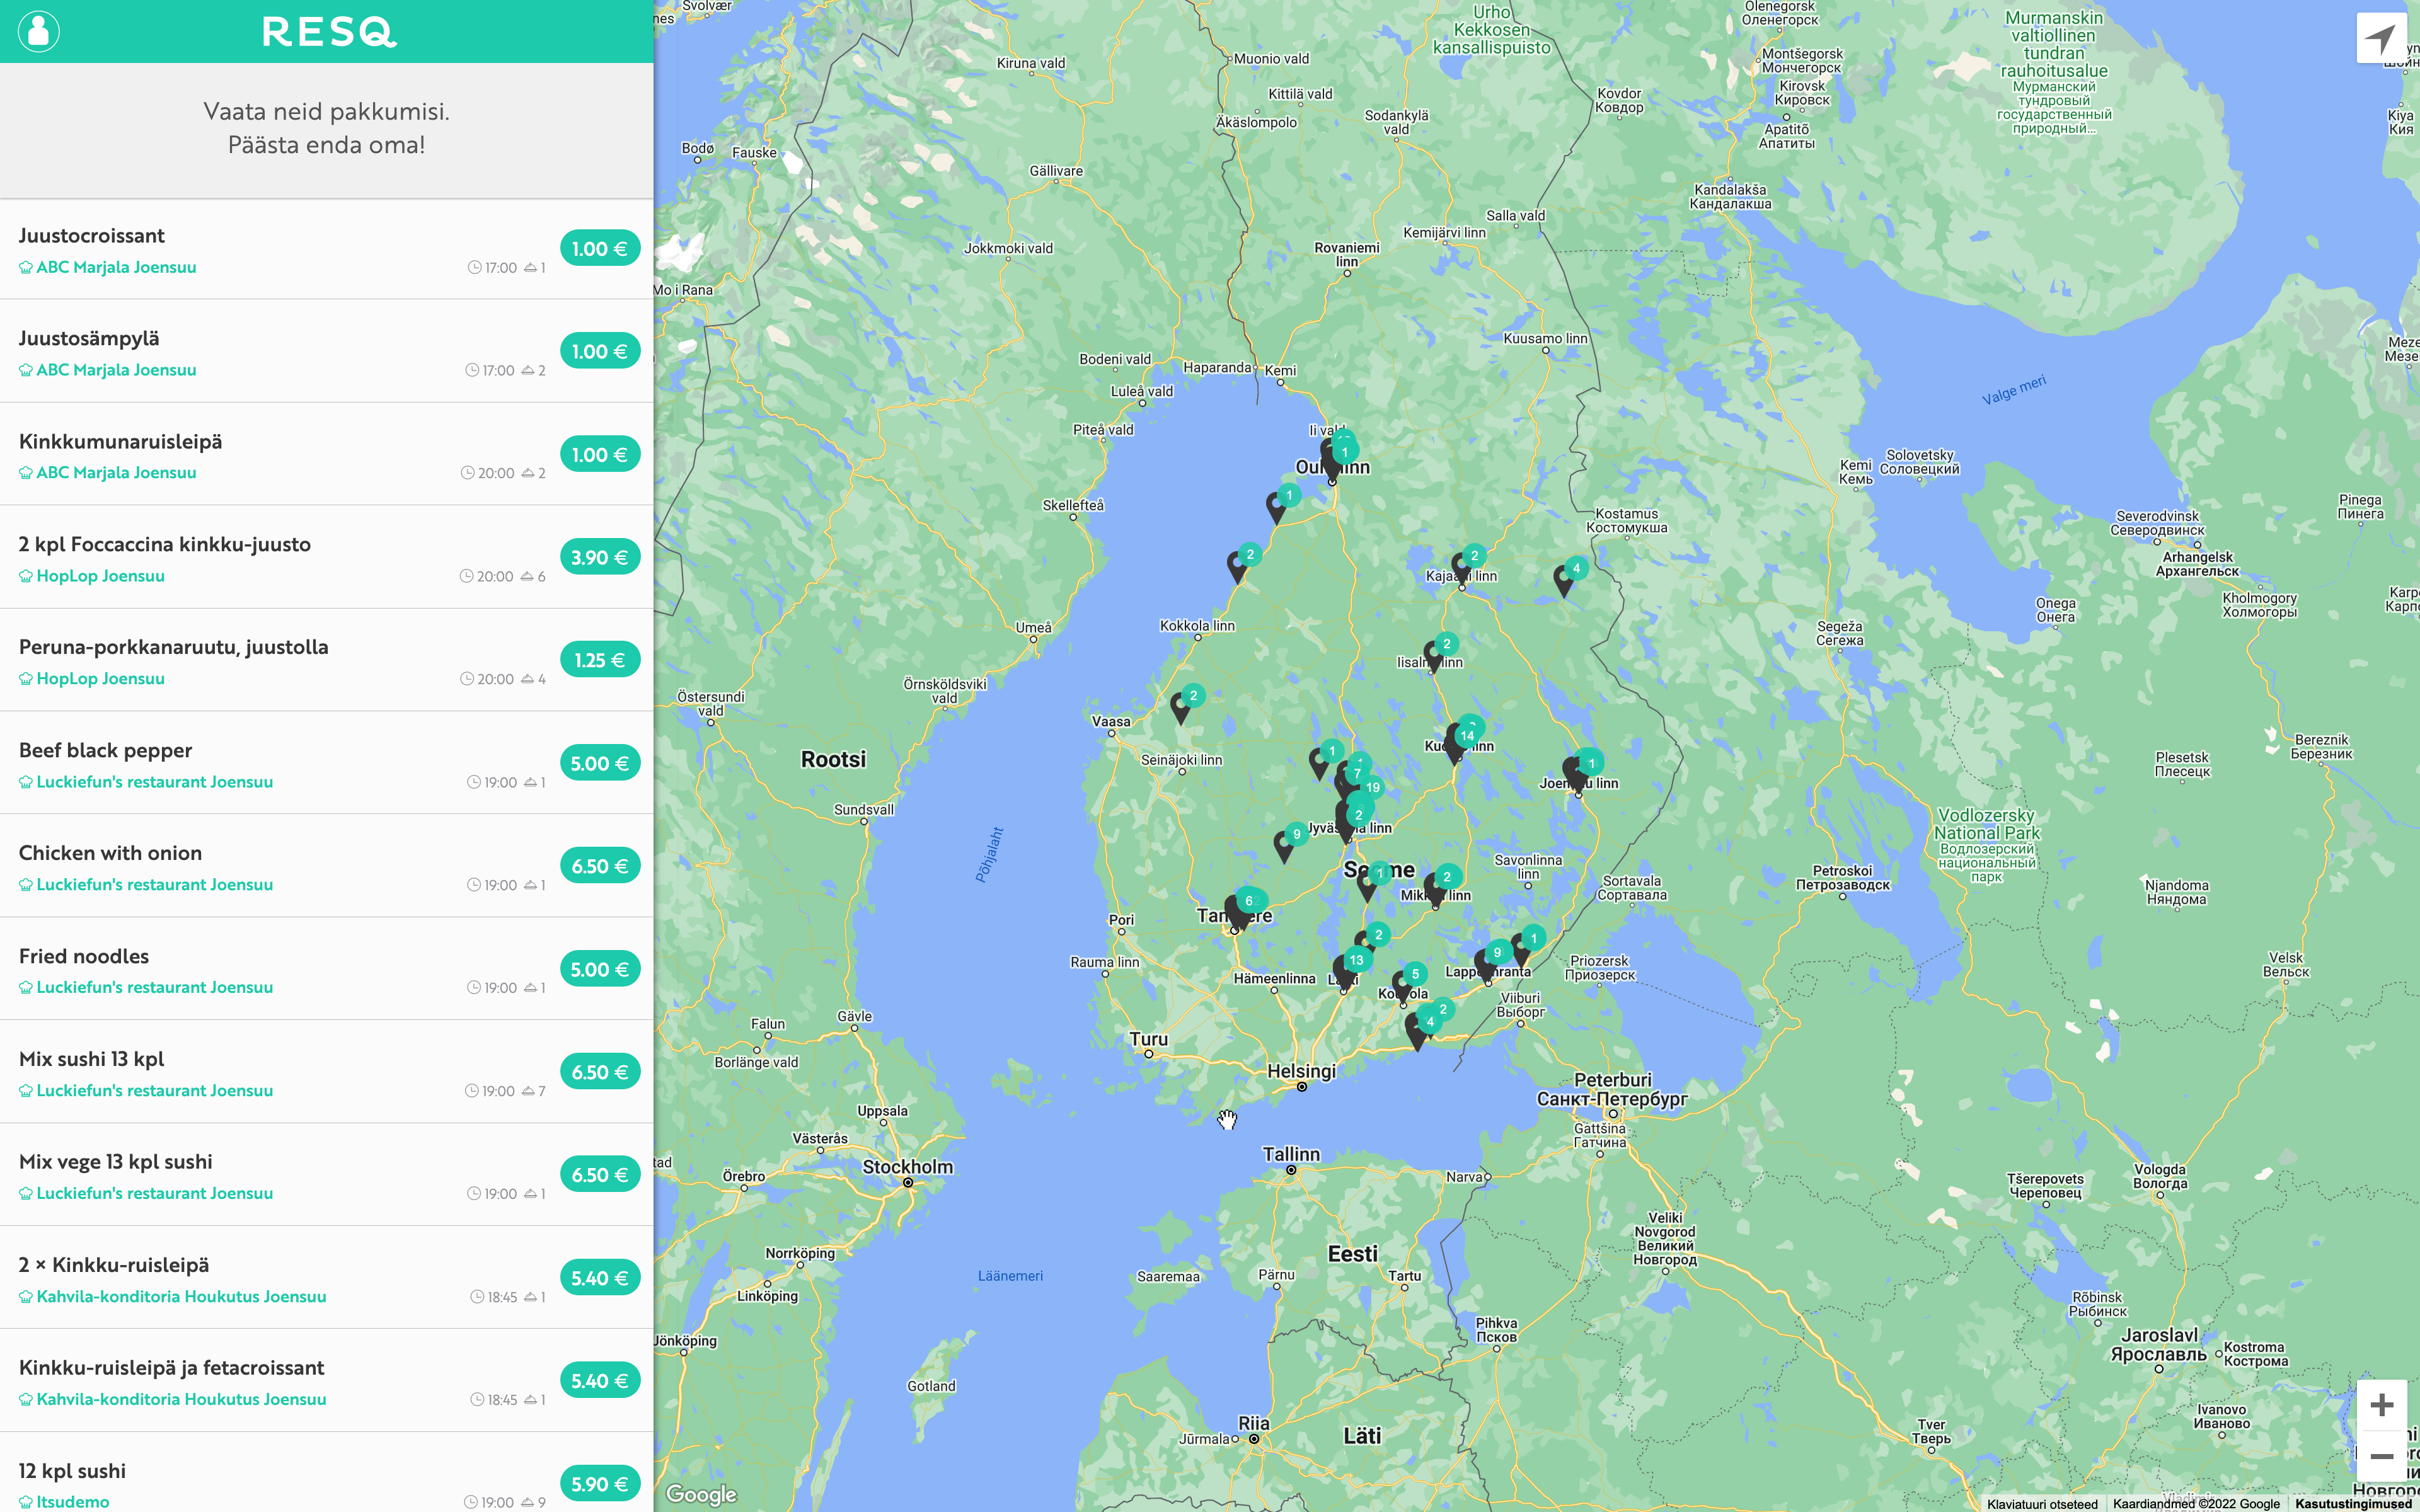
\includegraphics[width=1\linewidth,height=\textheight,keepaspectratio]{./images/design/resq-club.png}

}

\caption{ResQ Club saves food waste by selling left-over foods cheaply}

\end{figure}%

\def\pandoctableshortcapt{Food Saving Apps}

\begin{longtable}[]{@{}
  >{\raggedright\arraybackslash}p{(\linewidth - 2\tabcolsep) * \real{0.3611}}
  >{\raggedright\arraybackslash}p{(\linewidth - 2\tabcolsep) * \real{0.6389}}@{}}
\caption[Food Saving Apps]{Food saving apps}\tabularnewline
\toprule\noalign{}
\begin{minipage}[b]{\linewidth}\raggedright
Name
\end{minipage} & \begin{minipage}[b]{\linewidth}\raggedright
Description
\end{minipage} \\
\midrule\noalign{}
\endfirsthead
\toprule\noalign{}
\begin{minipage}[b]{\linewidth}\raggedright
Name
\end{minipage} & \begin{minipage}[b]{\linewidth}\raggedright
Description
\end{minipage} \\
\midrule\noalign{}
\endhead
\bottomrule\noalign{}
\endlastfoot
Karma & \\
ResQ Club & (Kristina Kostap, 2022) ResQ Club in Finland and Estonia for
reducing food waste by offering a 50\% discount on left-over restaurant
meals before they are thrown away. \\
Kuri & (Haje Jan Kamps, 2022) Less impact of food \\
Social media groups (no app) & \\
\end{longtable}

\let\pandoctableshortcapt\relax

As with any contentious issue, when it comes to food, people have
differing points of view. (Eriksson et al., 2023) discusses best
practices for reducing food waste in Sweden and (Röös et al., 2023)
identified 5 perspectives in a small study (n = 106) of views on the
Swedish food system.

\def\pandoctableshortcapt{Perspectives on the Food Systems in Sweden}

\begin{longtable}[]{@{}
  >{\raggedright\arraybackslash}p{(\linewidth - 2\tabcolsep) * \real{0.3611}}
  >{\raggedright\arraybackslash}p{(\linewidth - 2\tabcolsep) * \real{0.6389}}@{}}
\caption[Perspectives on the Food Systems in Sweden]{Perspective on food
systems in Sweden from (Röös et al., 2023).}\tabularnewline
\toprule\noalign{}
\begin{minipage}[b]{\linewidth}\raggedright
Perspective
\end{minipage} & \begin{minipage}[b]{\linewidth}\raggedright
Content
\end{minipage} \\
\midrule\noalign{}
\endfirsthead
\toprule\noalign{}
\begin{minipage}[b]{\linewidth}\raggedright
Perspective
\end{minipage} & \begin{minipage}[b]{\linewidth}\raggedright
Content
\end{minipage} \\
\midrule\noalign{}
\endhead
\bottomrule\noalign{}
\endlastfoot
\emph{``The diagnostic perspective''} & ``\emph{All hands on deck to fix
the climate''} \\
\emph{``The regenerative perspective''} & ``\emph{Diversity, soil health
and organic agriculture to the rescue''} \\
\emph{``The fossil-free perspective''} & ``\emph{Profitable Swedish
companies to rid agriculture and the food chain of fossil fuel''} \\
\emph{``The consumer-driven perspective''} & \emph{``A wish-list of
healthy, high-quality and climate-friendly foods''} \\
``The hands-on perspective'' & ``Tangible solutions within the reach of
consumers and the food industry'' \\
\end{longtable}

\let\pandoctableshortcapt\relax

\subsection{In Practice: Sustainability Begins in
Software}\label{in-practice-sustainability-begins-in-software}

Humans live in artificial environments where \emph{most things} are
designed by humans. Design encompasses most everything in our daily
lives. The \emph{experiences} we take part in are increasingly created
based on some type of data. \emph{Digital Sustainability} refers to the
idea that \emph{digital} enables \emph{sustainability}. Information
pertaining to emissions would flow through the economy not unlike the
carbon cycle itself.

Designing user interfaces for sustainable interactions means
incorporating data and tools to enable designers to make decisions which
reduce the emissions of their designs. Software is key to building more
sustainable products, already for decades (B. B. Gupta et al., 2023).
Increasingly, AI-assisted design is where sustainability starts: AI
provides the parameters for sustainability. Companies like AutoDesk have
introduced CO\textsubscript{2e} calculations inside their design
software, helping designers reduce material usage, energy consumption,
CO\textsubscript{2e} emissions, while increasing potential for reuse and
recyclability (Mike Haley, 2022). As AI tools and data quality improve,
a increasing number of parameters for deciding the suitable life cycle
design, will become available (Singh \& Sarkar, 2023).

(Pan \& Nishant, 2023) proposes 6 dimensions of \emph{AI} usage in
\emph{digital sustainability}. The chart is purely illustrative to
highlight the value of AI for sustainability; it's not based on numeric
metrics.

\begin{figure}

\centering{

\pandocbounded{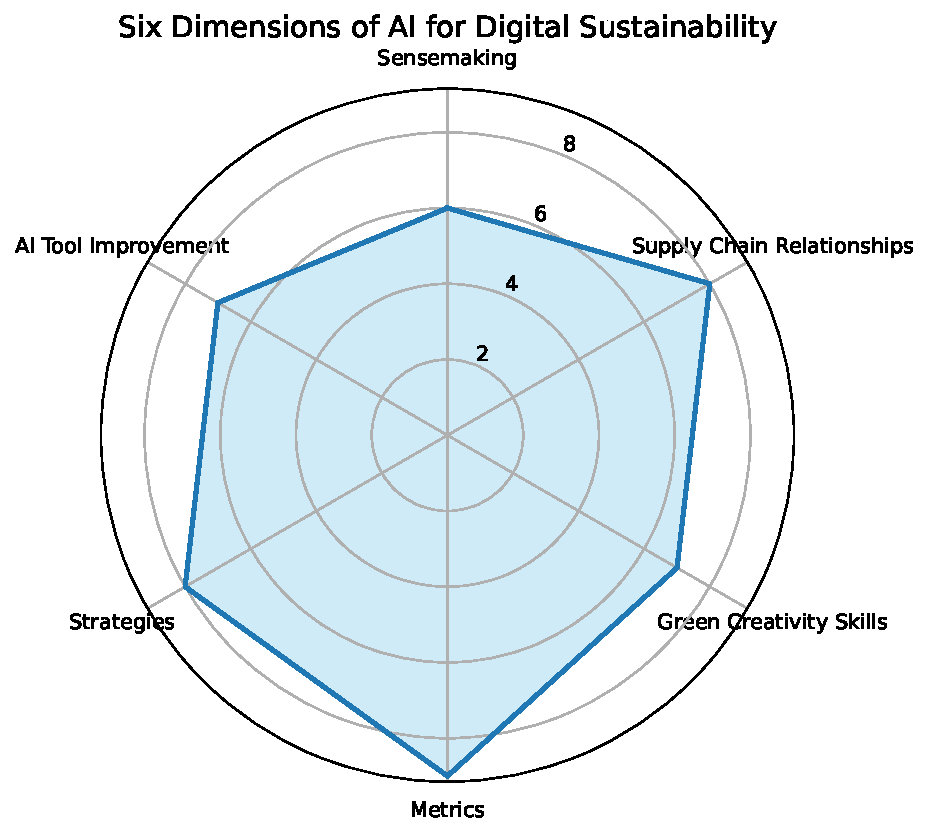
\includegraphics[keepaspectratio]{_thesis-nocite_files/figure-pdf/fig-ai-sust-six-output-1.pdf}}

}

\caption[AI Use in Sustainability]{\label{fig-ai-sust-six}AI Use in
Sustainability}

\end{figure}%

A crucial part of digital product design are \emph{design systems} to
keep consistency across the experience, and allowing teams to work
together towards a shared goal. Design systems accelerate development
and foster a cohesive user experience across products by reducing design
debt (M. Suarez et al., 2020). Yet the latest (Zeroheight Team, 2025)
survey (n = 294) shows that over 53\% of design systems are minimally
automated or not automated at all - and only 10\% of the designers
actively use AI, with 36\% having experimented with AI-driven design.
AI-usage for design across industry is uneven. Designers working at
Google have been designing in collaboratiom with AI for a while and
already in 2019 published the People + AI Guidebook, outlining best
practices for designing with AI - to make human-centered AI products
(\emph{People + {AI Guidebook}}, n.d.). In the enterprise context,
(Zimmerman et al., 2021) delves into the proposition of UX designers as
pioneers pushing AI-based adaptive UIs, as UX designers are the ones who
will best notice the broken workflows. All these findings underline,
there's still work to be done for the broader field of design to adopt
AI-based solution. Education is of the key, and one proposed path is
involving more young HCI designers in AI-oriented workshops to support
them building the future of UI/UX with AI (Battistoni et al., 2023).

\subsubsection{Data-Driven Design}\label{data-driven-design}

I believe it's possible to learn from the growth of digital platforms
and superapps to see how data-driven design could enable sustainability
to become mainstream. Sustainability touches every facet of human
existence and is thus an enormous undertaking. Making progress on
sustainability is only possible if there's a large-scale coordinated
effort by humans around the planet. For this to happen, appropriate
technological tools are required - simplifying the complexity of
sustainability.

Digital platforms are focused on \emph{growth design}, how to
\emph{attract} and \emph{retain} users. Superapps are the latter stage
of the economies of digital platforms, where previously vertically
targeted apps expand horizontally to provide an ever-increasing number
of services. For digital products (including superapps) the main
application of interaction design is for \emph{growth} in usage, how to
get more people (user journey and conversion funnels) to use the product
i.e user acquisition, retention, engagement, and monetization and keep
using it (retention and engagement), often optimizing on-boarding,
features, and personalization (Kende, 2023; Steger, 2019).

Platform economy companies popularized and expanded \emph{data-driven
design} in the service of growth marketing (also known colloquially as
\emph{growth hacking}). Capturing user data was part of this strategy
which enabled improving the products. Digital product design is
increasingly data-driven and digital platforms operate \emph{design as a
process} in a continuous feedback loop, where \emph{measurements},
\emph{experiments}, predictive analytics and personalization form a
data-drive design culture. As we humans go about our daily business,
governments and companies track our activities using various
technologies, which produces massive amounts of user interaction data.

Platform economy companies are the capture and use large amounts of data
from users. Data is useful for designing better products. Designing for
high retention (users keep coming back). Network Effects, the more
people use a platform, the more valuable it becomes. Platforms that
continuously add features (provided consumer legislation allows it) may
eventually evolve into superapps, which are useful for providing
services for a wide category of human needs. Bundling many services
under one super-brand. Superapps are possible thanks to Nudge, Economies
of Scale, Network Effects, Behaviour Design. Large Digital Platforms
have a very small number of workers relative to the number of users they
serve. This creates the necessity for using automation for both
understanding user needs and providing the service itself. Creating a
good product that's useful for the large majority of users depends on
\emph{Data-Driven Design.}

Design is as much about how it works as it's about the interface. There
are many approaches to design - from playful to practical to critical
and to data-driven. Nonetheless, many types of design share a common
goal designing for a good \emph{user experience} - except for those
design fields looking for \emph{shock value}. Digital product design can
be seen as a specific discipline under the umbrella of \emph{experience
design}. In (Michael Abrash, 2017) Laura Fryer, Meta Oculus augmented
reality incubation general manager, says as much: \emph{``People buy
experiences, not technology.''}

Personalization is the key to growth. The largest businesses today
(measured in number of users) design the whole user experience in order
to reach \emph{Scale}. Social apps require personalization because a
personal user experience will increase \emph{trust} and \emph{k-factors}
(sharing and inviting your friends) (Baron, 2023; B. Kim, 2023).
Intelligent Interfaces use interaction design to provide relevant and
personalized information in the right context and at the right time.
Popular consumer platforms strive to design solutions that feel
personalized at every touch point on the user journey (to use the
language of service design) at the scale of hundreds of billions of
users. Businesses care about Total addressable market (TAM), serviceable
addressable market (SAM), target audience (TA), and use hypothesis and
validation for iterating on features, to reach these lofty goals.

\subsubsection{Circular Design for a Circular
Economy}\label{circular-design-for-a-circular-economy}

The bible for Circular Economy, the \emph{``Cradle to Grave''} book was
released over 2 decades ago; change is slow, but change is happening
(McDonough \& Braungart, 2002).

Circular design is only possible if supply chains become circular as
well. (Hedberg \& Šipka, 2021) argues digitization and data sharing is a
requirement for building a circular economy. Yet, sometimes technology
fails. Nonetheless, many current technological hurdles can be overcome
by supply chain professionals who are experts in connecting supply
streams (Dull, 2021). (Oikos Denktank, 2021) argues circular design
requires new skills, one of which is circular material procurement.

To take a specific industry, digitization of mining systems allows to
enhance the reliability of supply chains, and provides better supply
chain transparency (CRM Alliance, 2020). This does not only include
tracking the critical raw materials, but also the social aspects
surround the mine. While this rarely makes the international media,
(Eerola, 2022) maps 20 ongoing mining and mineral-exploration disputes
in Finland, calling for systematic dispute monitoring, in order to
maintain a social license to operate.

The complexity of resource and delivery networks necessitates more
advanced tools to map supply chains (Knight et al., 2022). The COVID19
pandemic - and resulting blockages in resource delivery - highlighted
the need to have real-time visibility into supply chains (Finkenstadt \&
Handfield, 2021). Moreover, in the context of the EU Plastics Strategy,
\emph{``the European Commission has launched a pledge to increase the
use of recycled content to 10 million tons by 2025''}.

Already in 2020, a company founded to solve these exact issues,
Circularise, funded in part by the EU Commission H2020 SME Instrument,
developed a privacy-focused blockchain-based data exchange protocol for
tracing plastics across supply chains, aiming to boost transparency and
circularity across industries; their \emph{``Open Standard for
Sustainability and Transparency''} used ZK Proofs (a type of
cryptographic verification) for privacy preservation (a requirement of
many companies), while being able to prove the data is valid
(Circularise, 2020b, 2020a). Circularise is currently the market leader
in providing \emph{Digital Product Passports}, the value of which their
tagline \emph{``Connecting the Value Chain, One Product at a Time''}
explains quite clearly; in other words, the company aims to enable
circular economies by overcoming current limitations and communication
barriers in the value chain, by using an open blockchain-based
communications protocol (Stretton, 2022a).

It's important in which structure data is stored, affecting the ability
to efficiently access and manage the data while guaranteeing a high
level of data integrity, security, as well as energy usage of said data.
Blockchains are a type of shared database where the data is stored in
several locations with a focus on making the data secure and very
difficult to modify after it's been written to the database. Once data
is written to the blockchain, modifying it would require changing all
subsequent records in the chain and agreement of the majority of
validators who host a version of the database. Blockchain is the main
technology considered for accounting for the various inputs and complex
web of interactions between many participants inside the supply chain
networks.

Several startups are using to track source material arriving to the
factories and product movements from factories to markets and there are
hundreds of paper researching blockchain use in supply change operations
since 2017 (Dutta et al., 2020). Blockchains enable saving immutable
records into distributed databases (also known as ledgers). It's not
possible to (or extremely difficult) to change the same record, only new
records can be added on top of new ones. Blockchains are useful for data
sharing and auditing, as the time and place of data input can be
guaranteed, and it will be easier to conduct a search on who inputted
incorrect data; however the system still relies on correct data input.
As the saying goes, \emph{``garbage in, garbage out''}.

There are several technologies for tracking goods across the supply
chain, from shipping to client delivery. Data entry is a combination of
manual data input and automated record-keeping facilitated by sensors
and integrated internet of things (IoT) capabilities. For example
(Ashraf \& Heavey, 2023) describes using the Solana blockchain and
Sigfox internet of things (IoT) Integration for supply chain
traceability where Sigfox does not need direct access to internet but
can send low powered messages across long distances (for example
shipping containers on the ocean). (Van Wassenaer et al., 2023) compares
use cases for blockchains in enhancing traceability, transparency and
cleaning up the supply chain in agricultural products.

\def\pandoctableshortcapt{A Sample of Blockchain-based Supply Chain
Companies}

\begin{longtable}[]{@{}
  >{\raggedright\arraybackslash}p{(\linewidth - 4\tabcolsep) * \real{0.3288}}
  >{\raggedright\arraybackslash}p{(\linewidth - 4\tabcolsep) * \real{0.3288}}
  >{\raggedright\arraybackslash}p{(\linewidth - 4\tabcolsep) * \real{0.3425}}@{}}
\caption[A Sample of Blockchain-based Supply Chain Companies]{A sample
of blockchain-based supply chain companies as of summer
2023.}\tabularnewline
\toprule\noalign{}
\begin{minipage}[b]{\linewidth}\raggedright
Company
\end{minipage} & \begin{minipage}[b]{\linewidth}\raggedright
Link
\end{minipage} & \begin{minipage}[b]{\linewidth}\raggedright
Literature
\end{minipage} \\
\midrule\noalign{}
\endfirsthead
\toprule\noalign{}
\begin{minipage}[b]{\linewidth}\raggedright
Company
\end{minipage} & \begin{minipage}[b]{\linewidth}\raggedright
Link
\end{minipage} & \begin{minipage}[b]{\linewidth}\raggedright
Literature
\end{minipage} \\
\midrule\noalign{}
\endhead
\bottomrule\noalign{}
\endlastfoot
Ocean Protocol & oceanprotocol.com & \\
Provenance & provenance.io & \\
Ambrosius & ambrosus.io & \\
Modum & modum.io & \\
OriginTrail & origintrail.io & \\
Everledger & everledger.io & \\
VeChain & vechain.org & \\
Wabi & wabi.io & \\
FairFood & fairfood.org & \\
Bext360 & bext360.com & \\
SUKU & suku.world & (Miller, 2019) SUKU makes supply chains more
transparent yet seems to have pivoted away from supply chains \\
\end{longtable}

\let\pandoctableshortcapt\relax

Electronics contain valuable materials which can be recovered.
Meanwhile, (K. Liu et al., 2023) reports e-waste is growing 3\%-5\%
every year, globally. (Thukral \& Singh, 2023) identifies several
barriers to e-waste management among producers including lack of
awareness and infrastructure, attitudinal barriers, existing
\emph{informal} e-waste sector, and the need for an e-waste license.

(Builders for Climate Action, 2021) finds embodied carbon averages 250
kg CO\textsubscript{2}eq per m² of floor area for new Canadian homes,
varying from 175-400 kg CO\textsubscript{2}eq per m² based on building
material choices; one standard house emits 32--75 t
CO\textsubscript{2}eq; the authors believe however, using \emph{biogenic
materials} (e.g.~naturally grown materials including wood, bamboo,
straw, hemp, cork, and mycelium), could make the houses carbon negative,
storing 9--60 t CO\textsubscript{2}eq emissions - enough to meet the
2030 of the entire building sector.

\subsubsection{Tracking Ethics \& Cruelty: Transparent Factories and
Supply
Chains}\label{tracking-ethics-cruelty-transparent-factories-and-supply-chains}

\begin{quote}
``Secrecy is the linchpin of abuse of power\ldots its enabling force.
Transparency is the only real antidote.'' Glen Greenwald, Attorney and
journalist. (Greenwald, 2015)
\end{quote}

In the most general sense, supply chain transparency enables stakeholder
accountability (Circularise, 2018; Doorey, 2011; J. Fox, 2007). Products
are made from resources distributed across the planet and transported to
clients around the world which currently causes high levels (and
increasing) of greenhouse gases. \emph{``Transport greenhouse gas
emissions have increased every year since 2014''} (\emph{Climate Change
Mitigation}, 2023). Freight (transport of goods by trucks, trains,
planes, ships) accounts for 1.14 gigatons of CO\textsubscript{2}
emissions as per 2015 data or 16\% of total international supply chain
emissions (Yuqing Wang et al., 2022).

\def\pandoctableshortcapt{Share of CO\textsubscript{2}eq Emissions by
Type of Transport Globally}

\begin{longtable}[]{@{}ll@{}}
\caption[Share of CO~2~eq Emissions by Type of Transport Globally]{Share
of CO\textsubscript{2}eq emissions by type of transport globally
(Statista \& IEA, 2022).}\tabularnewline
\toprule\noalign{}
Type of Transport & Percentage \\
\midrule\noalign{}
\endfirsthead
\toprule\noalign{}
Type of Transport & Percentage \\
\midrule\noalign{}
\endhead
\bottomrule\noalign{}
\endlastfoot
Passenger cars & 39\% \\
\textbf{Medium and heavy trucks} & 23\% \\
\textbf{Shipping} & 11\% \\
\textbf{Aviation} & 9\% \\
Buses and minibuses & 7\% \\
Light commercial vehicles & 5\% \\
Two/three-wheelers & 3\% \\
Rail & 3\% \\
\end{longtable}

\let\pandoctableshortcapt\relax

In shipping, (Matthew Gore et al., 2022) reports the International
Maritime Organization (IMO) targets cutting CO\textsubscript{2}
equivalent emissions in shipping 50\% by 2050 compared to 2008. In
aviation, (Platzer, 2023), a scientist working on the Apollo space
program, calls for emergency action to develop \emph{green aviation}.

(Waters, 2015) analyzes the most effective strategies to improve animal
welfare and advance animal rights against a monopolistic producer
finding the most successful tactics to be (1) negotiation, (2) targeted
direct action, and (3) awareness campaigns condemning low-welfare
practices.

\subsection{Superapps Integrate Shopping, Savings, and
Investing}\label{superapps-integrate-shopping-savings-and-investing}

Superapps are the most prevalent across Asia, with China, South-East
Asia, Korea, Japan, and India leading the way, however newcomers in
Lating America and the Middle East are also making strides; meanwhile,
the US and Europe are lagging behind.

\def\pandoctableshortcapt{Global Overview of Superapps}

\begin{longtable}[]{@{}
  >{\raggedright\arraybackslash}p{(\linewidth - 14\tabcolsep) * \real{0.1250}}
  >{\raggedright\arraybackslash}p{(\linewidth - 14\tabcolsep) * \real{0.1250}}
  >{\raggedright\arraybackslash}p{(\linewidth - 14\tabcolsep) * \real{0.1250}}
  >{\raggedright\arraybackslash}p{(\linewidth - 14\tabcolsep) * \real{0.1250}}
  >{\raggedright\arraybackslash}p{(\linewidth - 14\tabcolsep) * \real{0.1250}}
  >{\raggedright\arraybackslash}p{(\linewidth - 14\tabcolsep) * \real{0.1250}}
  >{\raggedright\arraybackslash}p{(\linewidth - 14\tabcolsep) * \real{0.1250}}
  >{\raggedright\arraybackslash}p{(\linewidth - 14\tabcolsep) * \real{0.1250}}@{}}
\caption[Global Overview of Superapps]{Global overview of superapps (or
near-superapps) compiled from official company reports (IR, Press
Releases), news reports, and company websites; various metric types
(MAU, MTU, Annual Users, Customers, Registered Users) vary by company
reporting and are reduced into a single ``users'' metric for simplicity.
Each figure is sourced from official company reports, press releases, or
investor disclosures. If no recent official update was available (as in
the case of Alipay's 2020 figure), the latest known official figure is
provided. All values and dates reflect the latest data as of 2025. Data
sourced from (R. Brown, 2025; Careem, 2025; Ge \& Wei, Jul 20, 2020
06:42 PM; goto, 2023; Grab Holdings Limited, 2025; Jing, 2025; Kazanins,
2024; Laya, 2024; Philip Lee, 2025; LY Corporation, 2023; Mercado Libre,
2024; Nguyen \& Nguyen, 2023; Phocuswright, 2023; PhonePe, 2023; Pollo,
2025; Revolut, 2024b; Safaricom, 2024; Shinde, 2023, 2023; Tecent, 2024;
van Oost, 2024; Verma, 2024).}\tabularnewline
\toprule\noalign{}
\begin{minipage}[b]{\linewidth}\raggedright
\textbf{App}
\end{minipage} & \begin{minipage}[b]{\linewidth}\raggedright
Origin
\end{minipage} & \begin{minipage}[b]{\linewidth}\raggedright
\textbf{Metric}
\end{minipage} & \begin{minipage}[b]{\linewidth}\raggedright
Payments (Wallet)
\end{minipage} & \begin{minipage}[b]{\linewidth}\raggedright
Savings
\end{minipage} & \begin{minipage}[b]{\linewidth}\raggedright
Investing
\end{minipage} & \begin{minipage}[b]{\linewidth}\raggedright
\textbf{Users}
\end{minipage} & \begin{minipage}[b]{\linewidth}\raggedright
\textbf{Date}
\end{minipage} \\
\midrule\noalign{}
\endfirsthead
\toprule\noalign{}
\begin{minipage}[b]{\linewidth}\raggedright
\textbf{App}
\end{minipage} & \begin{minipage}[b]{\linewidth}\raggedright
Origin
\end{minipage} & \begin{minipage}[b]{\linewidth}\raggedright
\textbf{Metric}
\end{minipage} & \begin{minipage}[b]{\linewidth}\raggedright
Payments (Wallet)
\end{minipage} & \begin{minipage}[b]{\linewidth}\raggedright
Savings
\end{minipage} & \begin{minipage}[b]{\linewidth}\raggedright
Investing
\end{minipage} & \begin{minipage}[b]{\linewidth}\raggedright
\textbf{Users}
\end{minipage} & \begin{minipage}[b]{\linewidth}\raggedright
\textbf{Date}
\end{minipage} \\
\midrule\noalign{}
\endhead
\bottomrule\noalign{}
\endlastfoot
微信 \textbf{/ WeChat (Tencent)} & China & Monthly Active Users (MAU)
combined 微信 (China) \& WeChat (International) & Yes & Yes & Yes & 1,4
billion & 2024 \\
支付寶 \textbf{Alipay (Ant Group)} & China & Annual Active Users (AAU) &
Yes & Yes & Yes & 1.3 billion & 2020 \\
美團 \textbf{Meituan} & China & Annual Transacting Users (ATU) & Yes &
No & No & 700 million & 2024 \\
\textbf{PhonePe} & India & Registered Users (Lifetime) & Yes & Yes & Yes
& 500 million & 2023 \\
\textbf{LINE} & Japan & Monthly Active Users (MAU) & Yes & Yes & Yes &
200 million & 2023 \\
\textbf{Tata Neu} & India & Members & Yes & Yes & No & 27 million &
2023 \\
\textbf{Nubank} & Brazil & Customers & Yes & Yes & Yes & 114 million &
2024 \\
\textbf{Zalo} & Vietnam & Monthly Active Users (MAU) & Yes & No & No &
75 million & 2023 \\
\textbf{Paytm} & India & Monthly Transacting Users (MTU) & Yes & Yes &
Yes & 100 million & 2023 \\
\textbf{M-Pesa} & Kenya & Active Customers & Yes & Yes & No & 34 million
& 2024 \\
\textbf{Mercado Pago} & Argentina & Monthly Active Users (MAU) & Yes &
Yes & Yes & 61 million & 2023 \\
\textbf{PicPay} & Brazil & Active Customers & Yes & Yes & Yes & 35
million & 2023 \\
\textbf{Cash App (Block)} & USA & Monthly Active Users (MAU) & Yes & Yes
& Yes & 56 million & 2023 \\
\textbf{KakaoTalk} & Korea & Monthly Active Users (MAU) & Yes & Yes &
Yes & 48 million & 2024 \\
\textbf{GoTo (Gojek/Tokopedia)} & Indonesia & Annual Transacting Users
(ATU) & Yes & Yes & Yes & 51 million & 2023 \\
\textbf{Revolut} & UK & Customers & Yes & Yes & Yes & 50 million &
2024 \\
\textbf{Careem} & UAE (Aqcuired by US-based Uber and Etisalat but still
keeps a separate brand) & Customers & Yes & No & No & 70 million &
2024 \\
\textbf{Grab} & Singapore / Malaysia & Monthly Transacting Users (MTU) &
Yes & Yes & No & 41 million & 2024 \\
\textbf{Rappi} & Colombia & Users & Yes & Yes & No & 30 million &
2023 \\
\end{longtable}

\let\pandoctableshortcapt\relax

Uber is creating an all-purpose platform for travel; only 4.1\% of rides
were electric (Levy, 2023). In the UK, Uber launched and option to book
flights, moving to a door-to-door travel solution where the same app
brings you from home to the airport, the flight, and your final
destination (Uber UK, 2023).

\def\pandoctableshortcapt{Not Quite Superapps}

\begin{longtable}[]{@{}
  >{\raggedright\arraybackslash}p{(\linewidth - 12\tabcolsep) * \real{0.1429}}
  >{\raggedright\arraybackslash}p{(\linewidth - 12\tabcolsep) * \real{0.1429}}
  >{\raggedright\arraybackslash}p{(\linewidth - 12\tabcolsep) * \real{0.1429}}
  >{\raggedright\arraybackslash}p{(\linewidth - 12\tabcolsep) * \real{0.1429}}
  >{\raggedright\arraybackslash}p{(\linewidth - 12\tabcolsep) * \real{0.1429}}
  >{\raggedright\arraybackslash}p{(\linewidth - 12\tabcolsep) * \real{0.1429}}
  >{\raggedright\arraybackslash}p{(\linewidth - 12\tabcolsep) * \real{0.1429}}@{}}
\caption[Not Quite Superapps]{Not quite super-app yet. Data sourced from
(D. C. Garcia, 2025a; Uber, 2025)}\tabularnewline
\toprule\noalign{}
\begin{minipage}[b]{\linewidth}\raggedright
App
\end{minipage} & \begin{minipage}[b]{\linewidth}\raggedright
Origin
\end{minipage} & \begin{minipage}[b]{\linewidth}\raggedright
Metric
\end{minipage} & \begin{minipage}[b]{\linewidth}\raggedright
Payments (Wallet)
\end{minipage} & \begin{minipage}[b]{\linewidth}\raggedright
Savings
\end{minipage} & \begin{minipage}[b]{\linewidth}\raggedright
Investing
\end{minipage} & \begin{minipage}[b]{\linewidth}\raggedright
Users (2025)
\end{minipage} \\
\midrule\noalign{}
\endfirsthead
\toprule\noalign{}
\begin{minipage}[b]{\linewidth}\raggedright
App
\end{minipage} & \begin{minipage}[b]{\linewidth}\raggedright
Origin
\end{minipage} & \begin{minipage}[b]{\linewidth}\raggedright
Metric
\end{minipage} & \begin{minipage}[b]{\linewidth}\raggedright
Payments (Wallet)
\end{minipage} & \begin{minipage}[b]{\linewidth}\raggedright
Savings
\end{minipage} & \begin{minipage}[b]{\linewidth}\raggedright
Investing
\end{minipage} & \begin{minipage}[b]{\linewidth}\raggedright
Users (2025)
\end{minipage} \\
\midrule\noalign{}
\endhead
\bottomrule\noalign{}
\endlastfoot
Uber & USA & Users per month & No (Only for ride-hailing) & No & No &
171 million \\
Bolt & Estonia & Lifetime users & No (Only for ride-hailing) & No & No &
200 million \\
\end{longtable}

\let\pandoctableshortcapt\relax

Superapps offer a platform with key infrastructure such as payments
already included, where ecosystem of mini-apps thrive (Heath, 2021;
Perri, 2022). Alipay, originally a payments' app, has build the digital
infrastructure to provide thousands of services to billions of users
across China. 59 million people use 支小寶 (Zhixiaobao), an Al-based
assistant inside of Alipay, which can order taxis and meals, but also
interact with the Ant Bridge, Ant Bridge, Ant Fortune and Ant Insurance
services inside Alipay (Finextra, 2024). (Vecchi \& Brennan, 2022)
discusses the strategies Chinese apps are taking to expand to
international markets. (Giudice, 2020) finds WeChat has had a profound
impact on changing China into a cashless society, underlining how one
mobile app can transform social and financial interactions of an entire
country. (Shabrina Nurqamarani et al., 2020) discusses the system
consistency and quality of South-East Asian superapps Gojek and Grab.

Superapps are honeypots of data that is used for many types of behavior
modeling. Guido Becher from Rappi defines their super-app as
\emph{``customer-centric high frequency multi-vertical ecosystem''} this
enables cross-promotion, for example a hotel in Argentina targeted
people who buy almond milk on Rappi with their offer of a yoga retreat
(Phocuswright, 2023; G. Suarez et al., 2021) suggests using alternative
data from super-apps to estimate user income levels, including 4 types
of data: \emph{Personal Information}, \emph{Consumption Patterns},
\emph{Payment Information}, and \emph{Financial Services}. (Roa et al.,
2021) finds super-app alternative data is especially useful for
credit-scoring young, low-wealth individuals. However, data privacy is
always a concern. For instance, Kakao Pay was found guilty of
mishandling 40 million users' data by handing it over to Alipay without
user consent; Alipay owns a 32 percent stake in Kakao Pay (K. Lee,
2024).

There are also many aspiring superapps, companies which aspire to build
multi-vertical platforms but are hindered by various challenges.
Telegram integrates Web3 apps into the chat and supports investing into
cryptocurrencies without ever understanding the complex technology of
wallets. (Pylarinou, 2024). Likewise, LINE is integrating Web3
technologies based on the Kaia blockchain to provide decentralized
mini-apps (dapps) for the LINE chat userbase and integrates with the
LINE Pay wallet for financial interactions (Hintzy, 2025).

\emph{Platform Economy} marketplace companies like Airbnb and Uber,
among many others, match demand to offer, which in the process can
optimize how our cities work. The massive amounts of data generated by
these companies are used by smart cities to re-design their physical
environments, such as the collaboration between Bolt and the city of
Seville in Spain (Bolt, 2025). (Orozco et al., 2020) shows how important
data is for bicycle-network growth; in Budapest, small targeted
investments combined with data-driven algorithmic strategies, boosted
connectivity greatly above baseline approaches. Sustainable urban
transportation networks require building infrastructure that supports
eco-friendly modes of transportation - sidewalks, bicycle paths,
streets, rails, - while encouraging a lively movement and socio-economic
life in cities. Likewise, Google Environmental Insights Explorer enables
local governments (cities) to measure CO\textsubscript{2}eq emissions
and enact environmental policies that optimize city functions such as
traffic flows (\emph{Methodology - {Google Environmental Insights
Explorer} - {Make Informed Decisions}}, n.d.; Nicole Lombardo, 2021).
Several cities such as Tokyo, Shenzhen (深圳), and Paris have
voluntarily set carbon emissions caps (Koike, 2018; W. Song, 2025;
Zhijian, 2023). Integration with sustainability-services may help cities
achieve these goals faster.

\def\pandoctableshortcapt{Platform Economy Concepts}

\begin{longtable}[]{@{}
  >{\raggedright\arraybackslash}p{(\linewidth - 4\tabcolsep) * \real{0.2639}}
  >{\raggedright\arraybackslash}p{(\linewidth - 4\tabcolsep) * \real{0.3333}}
  >{\raggedright\arraybackslash}p{(\linewidth - 4\tabcolsep) * \real{0.4028}}@{}}
\caption[Platform Economy Concepts]{Platform economy concepts from (Chen
et al., 2012; Katz \& Shapiro, 1985; Oinas-Kukkonen \& Harjumaa, 2009;
Tiwana et al., 2010).}\tabularnewline
\toprule\noalign{}
\begin{minipage}[b]{\linewidth}\raggedright
Platform Economy Enablers
\end{minipage} & \begin{minipage}[b]{\linewidth}\raggedright
Pros
\end{minipage} & \begin{minipage}[b]{\linewidth}\raggedright
Cons
\end{minipage} \\
\midrule\noalign{}
\endfirsthead
\toprule\noalign{}
\begin{minipage}[b]{\linewidth}\raggedright
Platform Economy Enablers
\end{minipage} & \begin{minipage}[b]{\linewidth}\raggedright
Pros
\end{minipage} & \begin{minipage}[b]{\linewidth}\raggedright
Cons
\end{minipage} \\
\midrule\noalign{}
\endhead
\bottomrule\noalign{}
\endlastfoot
Network effects & The more people use a platform, the more valuable it
becomes both for the company and the user. & Data is not portable or
difficult to migrate. You can't leave because you'll lose the audience.
There's a lock-in effect. \\
Scalability & & \\
Data-driven Design & & \\
Behaviour Design & & \\
\end{longtable}

\let\pandoctableshortcapt\relax

(Cuppini et al., 2022) give a historical overview of how the rise of
digital platforms, taking an expansive point of view, all the way from
linear \emph{Fordism}, the development of capitalism, through platform
economy and the app-based logistics' revolution, which can provide data
for circular economies to happen in a city; reshaping the cities through
data-sharing with stakeholder from the citizens, to urban planner and
policy-makers - not without conflict, as there is often tension between
multiple perspectives.

\subsubsection{Personalization: Engineering
Persuasion}\label{personalization-engineering-persuasion}

In 2010, (IxDF, n.d.; Kolko \& Connors, 2010) believed \emph{Interaction
Design} is still an emerging (and changing) field, and there are many
versions of definitions. Instead of spending a lot of space trying to
define the limits of the field here, I prefer to simply say
\emph{interaction design is about creating a connection between the
product and the user}, and focus on the tools of an interaction
designer, which may be helpful for the goal of designing a
sustainability-focused financial AI assistant (the stated goal of this
research). And as what I'm designing here is an AI, the focus of the
interaction design will be the interaction between the human and the AIs
(possibly plural).

Kazuo Ishiguro's book \emph{``Klara and the Sun''} describes the nuanced
psychology of human-AI relations, flipping the script, narrating the
story through the eyes of the AF (artificial friend) - Klara, - who
(that?) describes the feeling of loneliness of a robot; the story offers
a cautionary counterpoint, illustrating how even the most loyal and
emotionally attuned AI companion could be perceived as uncanny or
insufficiently human (at least, this is how it happens in the book);
this example, while fictional, underscores the delicate balance required
when designing AI companions for sustainability: persuasion must feel
personal, but not performative (Ishiguro, 2021; Life Lessons From Books,
2023; Waterstones, 2021).

AI labs are putting a lot of effort into engineering likable AIs,
working on honesty of the models, teaching them to convey their own
uncertainty (Anthropic, 2024a, 2024b); Which sometimes can go wrong.
ChatGPT-4o overnight became your biggest fan, which users found
annoying; the abrupt shift to an overly enthusiastic persona drew user
backlash (Mollick, 2025). And it also felt jarring, if one already got
used to a certain persona - and then it suddenly changed.

\begin{quote}
\emph{``Interaction design isn't about how interfaces behave, it's about
how people behave, and then adapting technology accordingly.''} -
(UXPin, 2020)
\end{quote}

(Linden, 2021) from Meta's Artificial Intelligence team (which provides
AI services to Facebook, Instagram, etc.), reframes \emph{AI design} as
a long-game alignment job: instead of thinking UI-only, designers focus
on foresight, translating fuzzy, emerging patterns found in research,
into product concepts that could benefit real people's lives 2-3 years
in the future, when the technology matures; the AI designer has five
missions: (1) create proof-of-concept demos (the author gives examples
of prototypes like ``AI suggesting a caption for an IG post; AI
suggesting where to buy shoes''), letting non-experts see what a new
model might do, (2) understand research findings to steer raw
computer-vision, speech or language breakthroughs toward human problems
(examples such as ``AI-based search for users with visual impairment,
where touching a photo would let AI describe it''), (3) imagine user
needs several years in the future and incubate AI-first products to meet
those needs, (4) craft data-collection workflows, and (5) design
internal tooling that helps engineers build on the platform. Likewise,
(Stephanie Donahole, 2021) explores the impact of AI on UX/UI design
itself, augmenting UX processes, such as analyzing large datasets for
research insights, including surveys and qualitative analyses, creating
flow diagrams and wireframes, translating design between formats and
levels of fidelity, and fundamentally enabling deep personalization of
the design, freeing up the design professional to focus on higher-level
tasks (such as the visioneering describe above).

The concept of \emph{Social Objects} is relevant for interaction design
as people need something to gather around and discuss feeling
emotionally connected and safe (Sharing.Lab, 2015). Increasingly, the
social objects may be AI-generated, with the specific goal on
\emph{prompting humans} (in reverse, of humans prompting AIs, as is the
norm now). Another part of the toolset for interaction designers is also
\emph{Narrative Design,} because humans also respond well to
\emph{storytelling}, making \emph{character design} relevant to
interactions. Stories help product designers focus on the
\emph{stickiness} of the product, meaning low attrition, meaning people
keep coming back (Aidin Ardjomandi, 2025).

This can mean that the product \emph{has character} or literally -
characters. Large language models are able to assume the personality of
any character that exists inside its training data, creating
opportunities for automated narrative design. (Appleton, 2023) pushes
for more creativity in UX for AI, calling chatbots the lazy and obvious
solution; there is much more to be done for integrating AI into UX.
(Alethea AI, 2021) discusses writing AI Characters, creating a
personality; stories start with a character. Noah Levin, one of the
first employees and VP of Design at Figma, the most popular digital
design app, believes AI is the next chapter in design, starting with
small experimental AI-based plugins to becoming a core design platform
capability, accelerating most design workflows (Figma, 2023).

The quality of AI-generated UX has improved rapidly. In 2020, less than
5 years ago (Parundekar, 2021)'s extensive guide on creating an AI
products warned that an 80\% accurate model would mean \emph{``1 in 5
user requests being unsatisfied''}, underlining that a 1-second delay
would break the UX flow for many users: AI performance should be linked
to UX metrics. It can be safely said, today's AI products can already
satisfy these requirements with ease.

Long before AI assistants, (Justin Baker, 2018) introduced the concept
of \emph{Red Route Analysis}, an user experience optimization idea
inspired by the public transport system of London, focusing on the
\emph{critical design paths} which capture over 90\% of users' actions.
Prioritizing the user journey of the most popular features is key to
driving business metrics (\emph{Interaction {Design} -- {How} to
{Evaluate Interaction Costs} and {Improve User Experience}}, 2021;
Oviyam™, 2019; Xuan, 2022). Yet, (Richard Yang, 2021) argues
\emph{``{[}i{]}nteraction design is more than just user flows and
clicks''}, underlining Miller's Law that the average human can keep no
more than 5--11 items in their working memory (and now AI is becoming
that memory).

\subsection{Open Data Enables
Interoperability}\label{open-data-enables-interoperability}

Data is the \emph{interface} between idle resources and retail demand,
which makes \emph{exchange of value} possible. Yet often data is
expensive, hard-to-get, and inaccessible. If done well, open data can
enhance interoperability and enable collaboration (\emph{What Is {Open
Data}?}, n.d.).

While not officially a member, Taiwan is a proponent of Open Government
Partnership (OGP), and has launched its Open Government National Action
Plan, promoting open data, information transparency, and expanding
inclusive public participation (Lab, 2021; Open Government Partnership,
2021). Taiwan's Government Open Data Platform (資料開放平臺), managed by
the Ministry of Digital Affairs, centralizes hundreds of datasets; from
spatial information to energy use (Ministry of Digital Affairs, 2024a).
Open Knowledge International's Global Open Data Index (GODI) ranked
Taiwan as number 1 in its global index in 2017; the project has since
been discontinued, so the ranking may be out of date in 2024 (Open
Knowledge Foundation, 2017).

\begin{figure}

\centering{

\pandocbounded{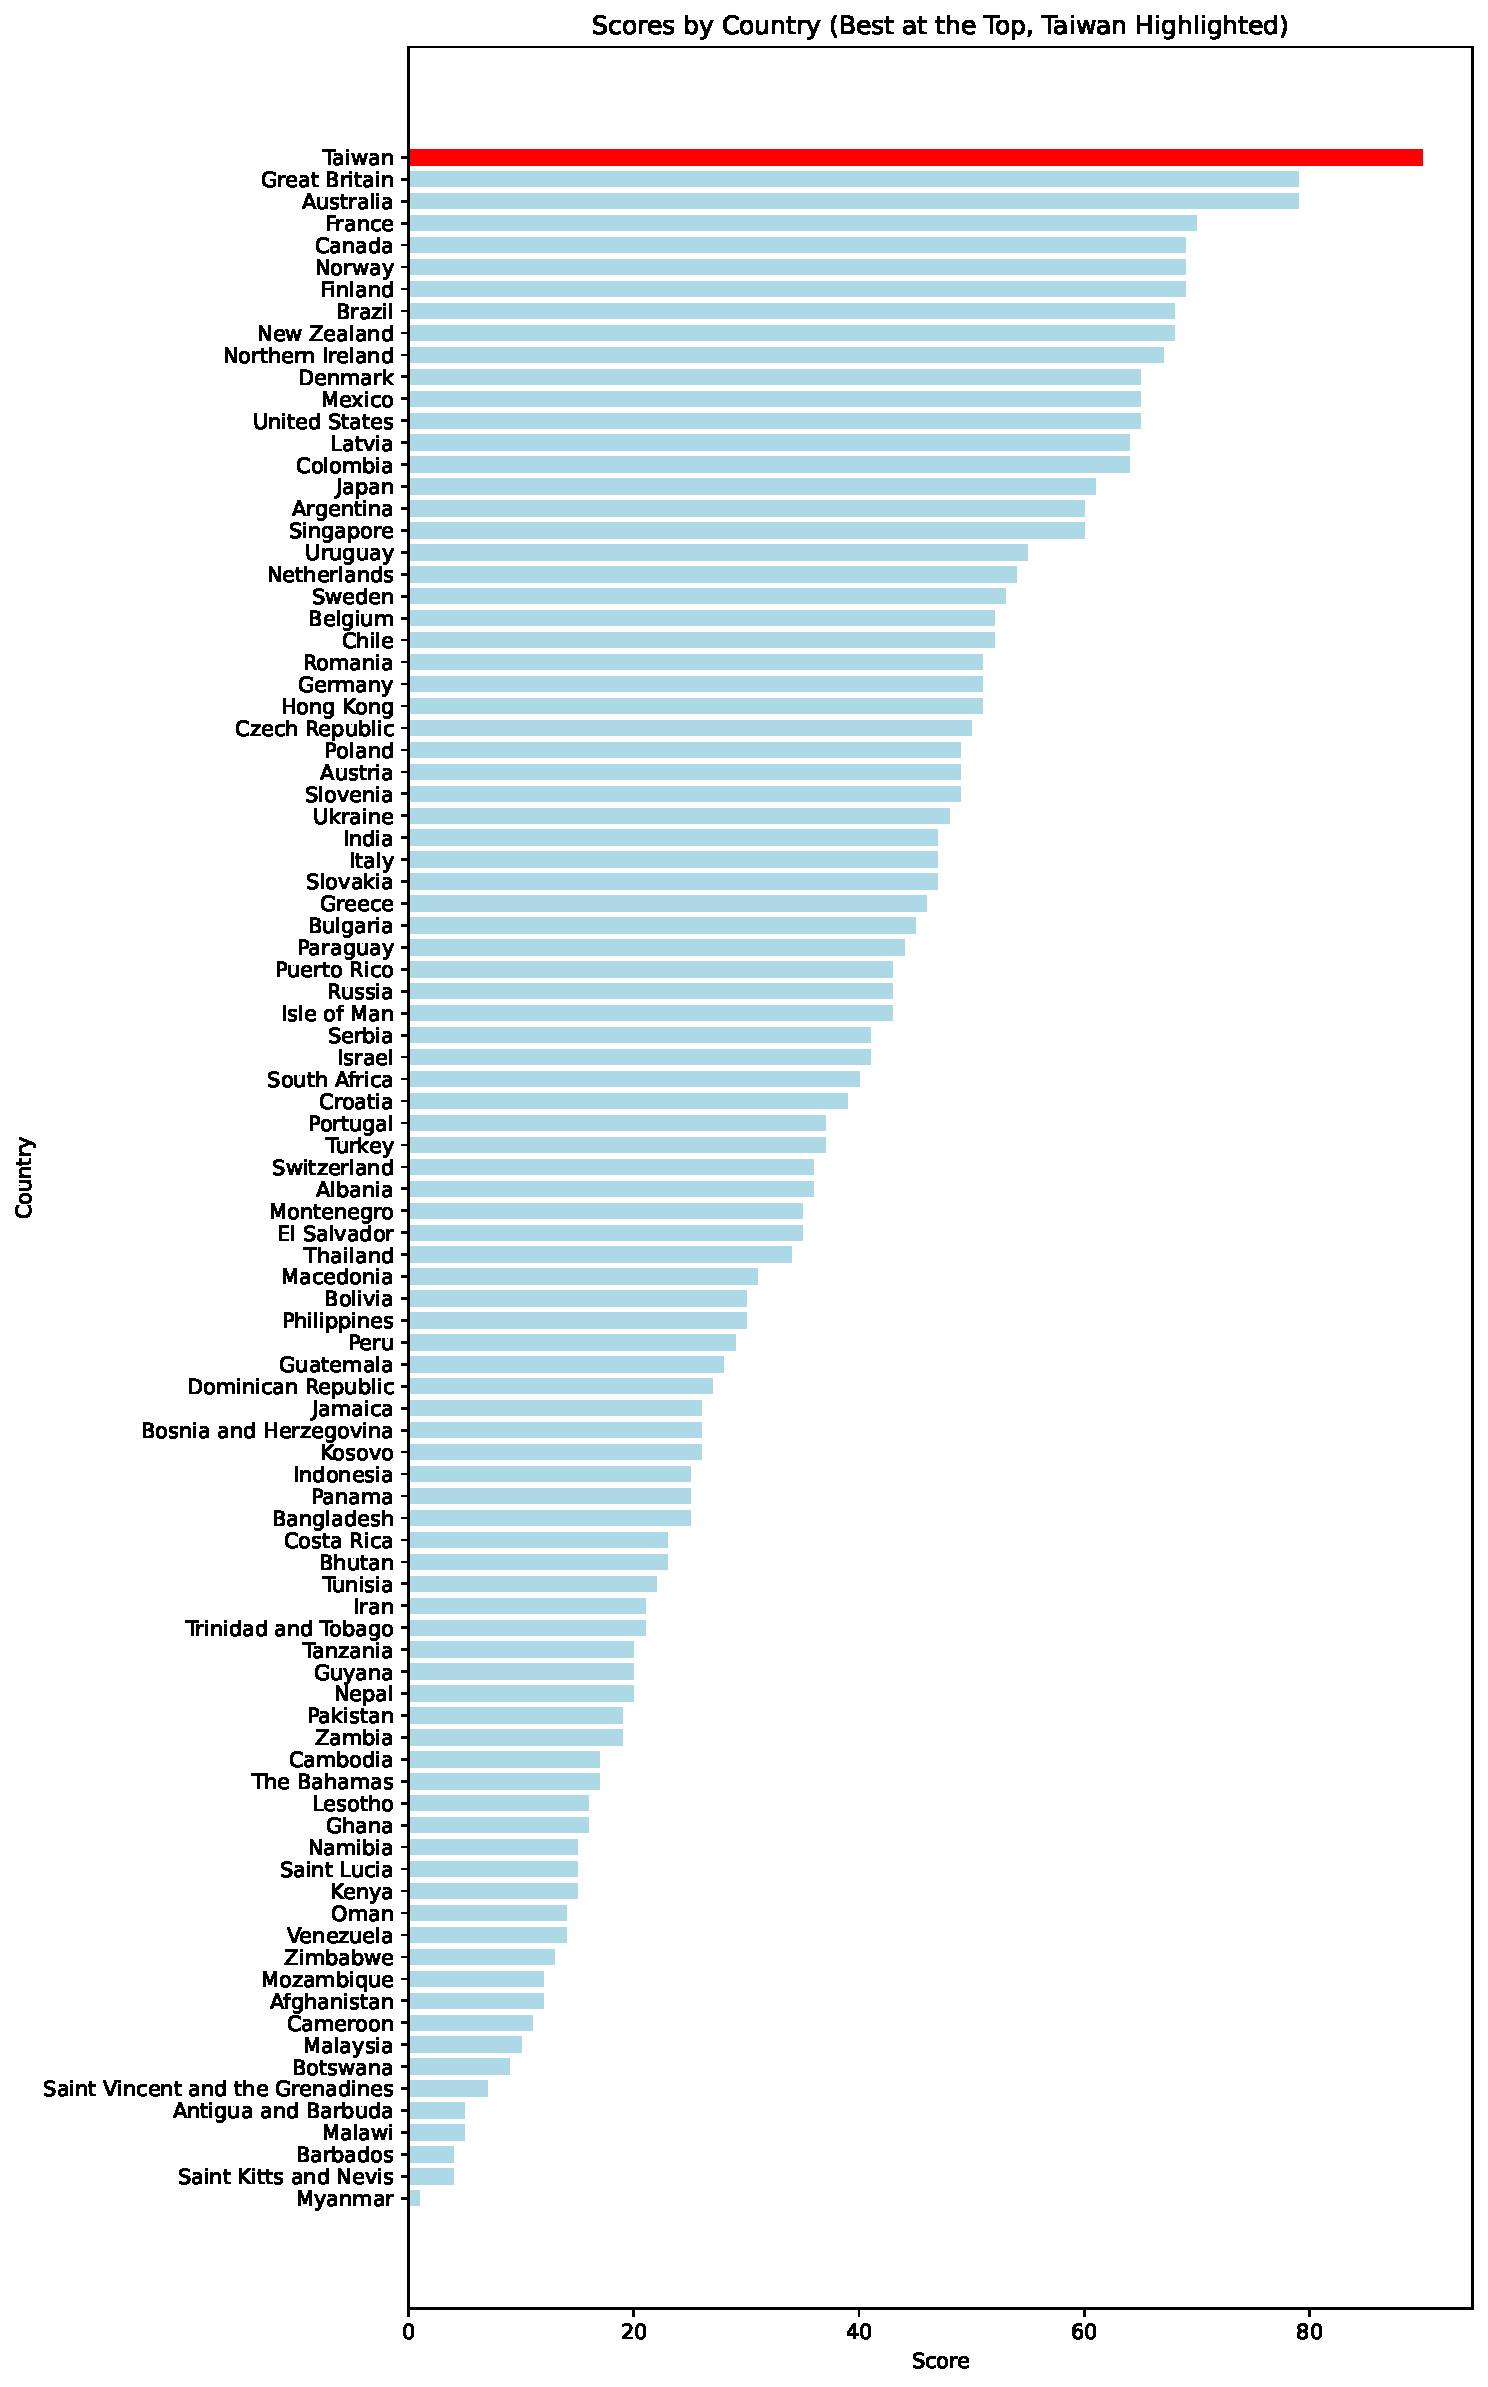
\includegraphics[keepaspectratio]{_thesis-nocite_files/figure-pdf/fig-open-data-index-output-1.pdf}}

}

\caption[Open Data Index]{\label{fig-open-data-index}Open Data Index}

\end{figure}%

Other indexes do not include Taiwan in the TOP 10.

\begin{figure}

\centering{

\pandocbounded{\includegraphics[keepaspectratio]{_thesis-nocite_files/figure-pdf/fig-open-data-compare-output-1.pdf}}

}

\caption[Alternative Open Data
Indexes]{\label{fig-open-data-compare}Alternative Open Data Indexes}

\end{figure}%

Data-driven design requires access to data, making the movement towards
\emph{open data sharing} very important. Some countries and cities are
better than others at sharing data openly.

\def\pandoctableshortcapt{Examples of Cities and Countries That Share
Data Openly}

\begin{longtable}[]{@{}ll@{}}
\caption[Examples of Cities and Countries That Share Data
Openly]{Examples of cities and countries that share data openly. Data
sourced from (Government of Malaysia, 2025; Monetary Authority of
Singapore, 2023; \emph{Sveriges Dataportal}, 2025)}\tabularnewline
\toprule\noalign{}
Country & Project \\
\midrule\noalign{}
\endfirsthead
\toprule\noalign{}
Country & Project \\
\midrule\noalign{}
\endhead
\bottomrule\noalign{}
\endlastfoot
Sweden & Swedish open data portal \\
Malaysia & Malaysian open data portal \\
Singapore & Singapore ESG open data platform \\
\end{longtable}

\let\pandoctableshortcapt\relax

To give a concrete example of the usefulness of open data, for instance,
the Open Data Portal of Malaysia shows a steady decline in Permanent
Reserved Forests (PRF) for anyone interested, without having to submit
any letter of request or communicate with officials; the data is just
directly accessible and includes a permissive license (of Malaysia,
2024). Likewise, in Singapore, the Monetary Authority has launched an
open data portal for ESG information, allowing anyone to delve into
environmental, social, and governmental topics (Monetary Authority of
Singapore, 2023).

\begin{figure}

\centering{

\pandocbounded{\includegraphics[keepaspectratio]{_thesis-nocite_files/figure-pdf/fig-mal-forests-output-1.pdf}}

}

\caption[Open Data As An Information Source for Environmental
Decline]{\label{fig-mal-forests}Open Data As An Information Source for
Environmental Decline}

\end{figure}%

\subsection{Context Design: Behavioral Nudges Towards Green Defaults in
Sustainable
Superapps}\label{context-design-behavioral-nudges-towards-green-defaults-in-sustainable-superapps}

For several decades, marketing researchers have been looking into how to
affect human behavior towards increasing purchase decisions in commerce,
both offline and online, which is why the literature on behavioral
design is massive. One of the key concepts is \emph{nudge}, first coined
in 2008 by the Nobel-winning economist Richard Thaler; nudges are based
on a scientific understanding of human psychology and shortcuts and
triggers that human brains use and leverages that knowledge to influence
humans in small but powerful ways (Thaler \& Sunstein, 2009).

The principles of nudge have also been applied to sustainability. For
example, a small study (n = 33) in the Future Consumer Lab in Copenhagen
by (Perez-Cueto, 2021) found that designing a ``dish-of-the-day'' which
was prominently displayed helped to increase vegetarian food choice by
85\%. Experiments by (Guath et al., 2022) focused on environmentally
friendly online purchases in Sweden (n = 200) suggest nudging can be
effective in influencing online shopping behavior towards more
sustainable options. A study of behavior change in Australia at large
university setting (N = 156) by (Novoradovskaya et al., 2021) found
nudging behavioral change had a significant effect and the author
suggested it may help to avoid some of the \emph{``16 billion paper
coffee cups are being thrown away every year''} globally (based on the
abstract - I was unable to access the full paper).

Google uses nudges in Google Flights and Google Maps, which allow
filtering flights and driving routes by the amount of
CO\textsubscript{2} emissions, as well as surfacing hotels with Green
Key and EarthCheck credentials, while promising new sustainability
features across its portfolio of products (Sundar Pichai, 2021). Such
tools are small user interface nudges which Google's research calls
\emph{digital decarbonization}, defined by (Implement Consulting Group,
2022) as \emph{``{[}m{]}aximising the enabling role of digital
technologies by accelerating already available digital solutions''}.

In (Kate Brandt \& Matt Brittin, 2022), Google's Chief Sustainability
Officer Kate Brandt set a target of ``at least 20-25\%''
CO\textsubscript{2} emission reductions in Europe to reach a net-zero
economy and the global announcement set a target of helping 1 billion
people make more sustainable choices around the world (Jeni Miles,
2022). In addition to end--users, Google offers digital decarbonization
software for developers, including the Google Cloud Carbon Footprint
tool and invests in regenerative agriculture projects (Google, 2023;
\emph{Inside {Google}'s Regenerative Agriculture Play {\textbar}
{Greenbiz}}, 2021). While Google has launched several climate-focused
initiatives, it missed its CO\textsubscript{2}eq reduction targets due
to growing need for AI models (Worthington, 2025a).

Google has launched eco--focused features across its range of products:
search improvements for finding hybrid and electric vehicles; green
routes for driving, in collaborating with local city governments
sourcing data from the traffic lights to provide AI‐powered
optimizations, which allows the map to suggest routes which would reduce
fuel use and idling, complete with charging‐station info; also, better
navigation for cyclists (showing scooter and bike‐share options)
(\emph{{Google mostrar{á} por defecto la ruta m{á}s 'verde' en su GPS y
ordenar{á} los vuelos seg{ú}n su impacto ambiental}}, 2021; Worthington,
2025a). (Sarah Perez, 2022) shows how Google added features to Flights
and Maps to filter more sustainable options. Yet, critics say updating
the CO\textsubscript{2}eq calculations' math means Google started hiding
emissions, which Google denies, pointing to higher accuracy of the
carbon emissions modeling instead ({``Google 'Airbrushes' Out Emissions
from Flying, {BBC} Reveals,''} 2022). Google's Nest Renew smart-home
product helped people shift heating, ventilation, and air conditioning
(HVAC) to use to cleaner grid times (with an optional subscription
service to match home electricity with renewable electricity credits);
in shopping searches, Google provides energy‐efficient appliance
recommendations, helping users choose lower‐impact products at the point
of purchase (Google, 2021; Justine Calma, Oct 6, 2021, 10:01 AM GMT+3).

\def\pandoctableshortcapt{Examples of CO\textsubscript{2} Visibility in
Google's Products}

\begin{longtable}[]{@{}
  >{\raggedright\arraybackslash}p{(\linewidth - 4\tabcolsep) * \real{0.3699}}
  >{\raggedright\arraybackslash}p{(\linewidth - 4\tabcolsep) * \real{0.2603}}
  >{\raggedright\arraybackslash}p{(\linewidth - 4\tabcolsep) * \real{0.3699}}@{}}
\caption[Examples of CO~2~ Visibility in Google's Products]{Examples of
CO\textsubscript{2} visibility in Google's products.}\tabularnewline
\toprule\noalign{}
\begin{minipage}[b]{\linewidth}\raggedright
Feature
\end{minipage} & \begin{minipage}[b]{\linewidth}\raggedright
Product
\end{minipage} & \begin{minipage}[b]{\linewidth}\raggedright
Nudge
\end{minipage} \\
\midrule\noalign{}
\endfirsthead
\toprule\noalign{}
\begin{minipage}[b]{\linewidth}\raggedright
Feature
\end{minipage} & \begin{minipage}[b]{\linewidth}\raggedright
Product
\end{minipage} & \begin{minipage}[b]{\linewidth}\raggedright
Nudge
\end{minipage} \\
\midrule\noalign{}
\endhead
\bottomrule\noalign{}
\endlastfoot
Google Maps AI suggests more eco-friendly driving routes (Mohit Moondra,
n.d.) & Google Maps & Show routes with lower CO\textsubscript{2}
emissions; reduce stopping by using data from traffic lights. \\
Google Flights suggests flights with lower CO\textsubscript{2} emissions
& Google Flights & Show flights with lower CO\textsubscript{2}
emissions \\
Wizzair Check carbon impact (\emph{Offset Your Flight with {WIZZ}},
n.d.) & WizzAir & Offset on Checkout \\
\end{longtable}

\let\pandoctableshortcapt\relax

\begin{figure}[H]

{\centering \includegraphics[width=1\linewidth,height=\textheight,keepaspectratio]{./images/design/flight-emissions.png}

}

\caption{Google's view of flight emissions}

\end{figure}%

(Wee et al., 2021) proposes 7 types of nudging technique based on an
overview of 37 papers which explore nudging people to be more
environmentally friendly.

\def\pandoctableshortcapt{Types of Nudge}

\begin{longtable}[]{@{}
  >{\raggedright\arraybackslash}p{(\linewidth - 2\tabcolsep) * \real{0.3611}}
  >{\raggedright\arraybackslash}p{(\linewidth - 2\tabcolsep) * \real{0.6389}}@{}}
\caption[Types of Nudge]{Types of nudge documented by (Wee et al.,
2021)}\tabularnewline
\toprule\noalign{}
\begin{minipage}[b]{\linewidth}\raggedright
Name
\end{minipage} & \begin{minipage}[b]{\linewidth}\raggedright
Technique
\end{minipage} \\
\midrule\noalign{}
\endfirsthead
\toprule\noalign{}
\begin{minipage}[b]{\linewidth}\raggedright
Name
\end{minipage} & \begin{minipage}[b]{\linewidth}\raggedright
Technique
\end{minipage} \\
\midrule\noalign{}
\endhead
\bottomrule\noalign{}
\endlastfoot
Prompting & Create cues and reminders to perform a certain behavior \\
Sizing & Decrease or increase the size of items or portions \\
Proximity & Change the physical (or temporal) distance of options \\
Presentation & Change the way items are displayed \\
Priming & Expose users to certain stimuli before decision-making \\
Labelling & Provide labels to influence choice (for example
CO\textsubscript{2} footprint labels) \\
Functional Design & Design the environment and choice architecture so
the desired behavior is more convenient \\
\end{longtable}

\let\pandoctableshortcapt\relax

(Acuti et al., 2023) makes the point that physical proximity to a
drop-off point helps people participate in sustainability and
metaphorical messaging alongside proximity can be powerful, enhancing
the ease of information processing. In a field study in Northern Italy,
a metaphor‐based message re-framed the factual statement ``1g of mercury
can pollute 1000L of water'' as ``7 bathtubs'', and 354000000L as ``140
Olympic swimming pools,'' (a projection of potential Italian mercury
pollution at current disposal rates), which significantly boosted
willingness to recycle mercury.

Alibaba's Ant Forest (螞蟻森林) has shown the potential gamified nature
protection, simultaneously raising money for planting forests and
building loyalty and brand recognition for their sustainable action,
leading the company to consider further avenues for gamification and
eco-friendliness.

\def\pandoctableshortcapt{Ant Forest Assisted Tree Planting - Growth
Story}

\begin{longtable}[]{@{}
  >{\raggedright\arraybackslash}p{(\linewidth - 6\tabcolsep) * \real{0.0857}}
  >{\raggedright\arraybackslash}p{(\linewidth - 6\tabcolsep) * \real{0.1857}}
  >{\raggedright\arraybackslash}p{(\linewidth - 6\tabcolsep) * \real{0.1857}}
  >{\raggedright\arraybackslash}p{(\linewidth - 6\tabcolsep) * \real{0.5429}}@{}}
\caption[Ant Forest Assisted Tree Planting - Growth Story]{Ant Forest
assisted tree planting; data compiled from (P. Cao \& Liu, 2023;
\emph{Over 600 {Million People Planted More Than} 326 {Million Trees}
via {Alipay Ant Forest} in {Five Years}}, 2021; UNFCCC, 2019; S. Wang et
al., 2022; X. Wang \& Yao, 2020; Z. Yang et al., 2018; B. Zhang et al.,
2022; F. Zhou et al., 2023; 张越熙, 2024; 李连环 \& 姜舒译, 2017; 胡群
\& 宋璠, 2024).}\tabularnewline
\toprule\noalign{}
\begin{minipage}[b]{\linewidth}\raggedright
Year
\end{minipage} & \begin{minipage}[b]{\linewidth}\raggedright
Users
\end{minipage} & \begin{minipage}[b]{\linewidth}\raggedright
Trees
\end{minipage} & \begin{minipage}[b]{\linewidth}\raggedright
Area
\end{minipage} \\
\midrule\noalign{}
\endfirsthead
\toprule\noalign{}
\begin{minipage}[b]{\linewidth}\raggedright
Year
\end{minipage} & \begin{minipage}[b]{\linewidth}\raggedright
Users
\end{minipage} & \begin{minipage}[b]{\linewidth}\raggedright
Trees
\end{minipage} & \begin{minipage}[b]{\linewidth}\raggedright
Area
\end{minipage} \\
\midrule\noalign{}
\endhead
\bottomrule\noalign{}
\endlastfoot
2016 & N/A & N/A & N/A \\
2017 & 230 million & 10 million & N/A \\
2018 & 350 million & 55 million & 6500 acres?? \\
2019 & 500 million & 100 million & 112,000 hectares / 66, 000
hectares? \\
2020 & 550 million & 200 million & 2,7 million acres? \\
2021 & 600 million & 326 million & N/A \\
2022 & 650 million & 400 million & 2 million hectares \\
2023 & 690 million & 475 million & N/A \\
2024 & N/A & 548 million & 3.87 million hectares \\
2025 & N/A & N/A & N/A \\
\end{longtable}

\let\pandoctableshortcapt\relax

\begin{figure}

\centering{

\pandocbounded{\includegraphics[keepaspectratio]{_thesis-nocite_files/figure-pdf/fig-ant-forest-growth-output-1.pdf}}

}

\caption[Growth of Ant Forest]{\label{fig-ant-forest-growth}Growth of
Ant Forest}

\end{figure}%

Ecosia is a search engine with an unconventional business models,
investing all its profits into planting trees, pouring €92 million into
climate action since 2009, planting 225 million trees worldwide (D. C.
Garcia, 2025b). The founder Christian Kroll recalls travelling in South
America in 2006 and being shocked to see vast areas of rainforests
converted into soy plantations, which inspired him to research the
causes of deforestation and start Ecosia; the company employs partners
around the world to improve soil, biodiversity, the water cycle,
reducing droughts and floods, and monitor the trees it plants (Hirsh,
2021).

New user interfaces hold some potential for sustainability improvements.
In particular, immersive communication technologies such as AR/VR hold
the potential to reduce business travel, if productive meetings can be
held online, reducing emissions. Likewise, visualizing large
architectural projects as well as simulating product design in various
industries can reduce cost by detecting problems in the 3D environment,
early on in the design process, especially for collaboration in teams
located all over the world (Varjo, 2025). Dynamic interfaces might
invoke a new, natural-interaction-focused design language, for taking
full advanced of extended reality (Hoang, 2022). First encouraging
findings from reconstructing language from fMRI readings (brain scans)
even show potential for enabling computers to directly read human minds;
contemporary AI models have already been shown capable of generating
full sentences from human thoughts (J. Tang et al., 2022).

The small screen estate space of mobiles phones and smartwatches
necessitates displaying content in a dynamic manner. Likewise, speaking
is one mode of interaction that's become increasingly possible as
machines learn to interpret human language. Virtual reality glasses
(called AR/VR or XR in marketing speak) need dynamic content because the
user is able to move around the environment. All these are multi-modal
communication questions that interaction design is called upon to solve.

\def\pandoctableshortcapt{Modes of Interaction}

\begin{longtable}[]{@{}l@{}}
\caption[Modes of Interaction]{Modes of Interaction}\tabularnewline
\toprule\noalign{}
Modes of Interaction \\
\midrule\noalign{}
\endfirsthead
\toprule\noalign{}
Modes of Interaction \\
\midrule\noalign{}
\endhead
\bottomrule\noalign{}
\endlastfoot
Writing \\
Speaking \\
Touching \\
Moving \\
Seeing \\
\end{longtable}

\let\pandoctableshortcapt\relax

\subsection{Learning from Quantified Self: Tracking Health and
Lifestyle}\label{learning-from-quantified-self-tracking-health-and-lifestyle}

An early example of how tracking personal data enables behavior change,
are health and lifestyle tracking apps. Research on \emph{personal data
tracking} also known as \emph{quantified self} or \emph{self-monitoring}
is abundant. There's substantial academic evidence indicating that
health tracking apps can have a measurable impact on user health
behaviors and increase positive health outcomes. Wearable devices
including the Apple Watch, Oura Ring, Fitbit and others, combined with
apps, help users track a variety of health metrics. Recently, npj
Biosensing even published a device from the MIT Media Lab that can track
cells inside the human body from a wrist-worn device (Jang et al., 2025;
Jarvis, 2025).

Apart from health, wearable devices have been used to track other
metrics such as physiological parameters of students at school to
determine their learning efficiency (Giannakos et al., 2020). Not only
can health metrics be tracking, but exposure to pollution as well as
personal carbon footprint, are all to some extent track-able (if not
traceable).

\subsubsection{Health and Fitness
Tracking}\label{health-and-fitness-tracking}

Tracking one's health and fitness is a familiar mode of \emph{quantified
self}, available to many smartwatch users - and even pretty much to
anyone who has a phone made in the past decade. Apple is a leader in
health tracking, releasing Apple Health in 2008 as an iOS 8 software
feature and the Apple Watch in 2015, filled with health-focused sensors
and features (Apple, 2022b). In 2022 Apple outlined plans for
\emph{``empowering people to live a healthier day,''} promising a new
set of health-features with every release, such as the rumored
temperature measurement inside of Apple AirPod earphones; and providing
most of this data to developers through Apple's HealthKit health metrics
APIs, which app builders can tap into (Apple, 2022a, 2022c).

Use of wearable devices enables one to be more aware of one's health.
(Saubade et al., 2016) finds health tracking is useful for motivating
physical activity. Blood glucose tracking is popular even for people
without diabetes, to optimize their daily activity, including sports
(\emph{Is Blood Sugar Monitoring Without Diabetes Worthwhile?}, 2021).
Smart toilets offer unobtrusive monitoring of urine for one's hydration
levels as well as deeper insights on biomarkers as well as renal and
nutritional health, through using sensor‐equipped seats (e.g.~Withings'
U-Scan), which create a daily stream of data useful for trend analysis
(Hermsen et al., 2023; Wagner \& Boiten, 2023). Companies like
NeuralLink are building devices to construct meaningful interactions
based only on brain waves (EEG) (Musk \& Neuralink, 2019).

Popular Strava sports assistant (over 100 million users) provides
activity tracking and feedback (Strava, 2022).

\begin{figure}[H]

{\centering \includegraphics[width=1\linewidth,height=\textheight,keepaspectratio]{./images/design/strava.png}

}

\caption{Popular Strava sports assistant provides run tracking and
feedback}

\end{figure}%

Sleep quality is an important aspect of both physical and mental health
and many devices and apps focus on helping people get enough high
quality sleep. There's plenty of academic literature on how physical
activity, as well as environmental aspects, such as air quality, affect
sleep (X. Liu et al., 2019) tracks how wearable data is used for
tracking sleep improvements from exercise. (Grigsby-Toussaint et al.,
2017) made use of sleep apps to construct humans behaviors also known as
\emph{behavioral constructs}.

Being conscious of one's mental health improves quality of life. (Tyler
et al., 2022) surveyed the use of self-reflection apps in the UK (n =
998) finding a variety of methods from physical journaling in notebooks
to smartphone-based note-taking apps, reviewing printed photo albums,
and other digital tools.

Tracking one's food intake helps to understand how healthy and
nutrient-rich is one's diet. (Ryan, 2022) uses the ``capability
methodology'' framework, developed by economist Amartya Sen and later
expanded by philosopher Martha Nussbaum, shifting focus from what people
have (e.g.~money, food, tools) to what they are able to do (human
capabilities), which is used in the context of this paper to evaluate
not only if the apps provide healthy food suggestions, but to what
extent they expand a user's freedom to live a healthy life; some forms
of nudging inside the apps can support users' goals however manipulative
or coercive tactics serve only the app developers' interests and are
ethically problematic - the paper emphasizes the need for interaction
design that respect users' freedom, consider diverse personal choices,
diverse bodies, cultures, and preferences, and environmental factors.

The Oura ring is an example of \emph{calm technology}, providing helpful
data without calling an attention to itself (Phelan, 2024). More
recently, Oura Ring launched an AI-advisor to help explain the health
data recorded by its device: deliver contextual and personalized
guidance, remember past interactions while emphasizing privacy, and
analyze both short- and long-term biometric trends (Team, 2025). There's
value in developing standardized fitness metrics, which different
digital health providers can use to create dashboards with comparable
data. Even with messy data, AI has a useful role as a translator between
different standards. OpenAI is collaborating with ex-Apple designer Jony
Ive, to bring such ambient AI devices to live, which they believe has
the potential for a new product category (WSJ News, 2025).

\subsubsection{Pollution Exposure
Tracking}\label{pollution-exposure-tracking}

Pollution exposure tracking may be considered a combination of health
tracking and sustainability tracking. I've been tracking my personal air
pollution exposure using the Atmotube Pro device attached to my
backpack.

\begin{figure}

\centering{

\pandocbounded{\includegraphics[keepaspectratio]{_thesis-nocite_files/figure-pdf/fig-air-pollution-personal-output-1.pdf}}

}

\caption[My Personal Exposure to Air
Pollution]{\label{fig-air-pollution-personal}My Personal Exposure to Air
Pollution}

\end{figure}%

The above chart shows my exposure to pollutants while traveling, ranked
from worst to best.

\subsubsection{Tracking Personal Sustainability and Carbon
Emissions}\label{tracking-personal-sustainability-and-carbon-emissions}

The above examples of tracking various aspects of health beg the
question if one could track personal sustainability similarly. We have a
limited carbon budget so calculating CO\textsubscript{2}eq-cost could be
expressly integrated into every activity.

Already in 2017, a project funded by the EU Horizon 2020 title
\emph{``Instant Gratification for Collective Awareness and Sustainable
Consumerism''} piloted the concept of \emph{``political consumerism''},
by enabling shoppers at 2 stores (Estonia and Austria) to experience
real-time, personalized sustainability ratings on nearby products (by
using a mobile app and bluetooth beacons to locate shoppers at shelf
level, while maintaining privacy); instead of isolated choices,
individual preferences were (environmental, health, political)
aggregated into a community ``sustainability signal''; the results
indicated a statistically significant increase in sustainability
awareness and some users praised the simplicity of the user interface
(Bennati \& Pournaras, 2018; \emph{Instant {Gratification} for
{Collective Awareness} and {Sustainable Consumerism}}, 2022; Klinglmayr
et al., 2017; Pournaras et al., 2016).

More recently, (Kommenda et al., 2022) describes an interactive demo of
Carbon Food Labels in the Financial Times, aimed at influence purchasing
behavior by displaying Life Cycle Assessment (LCA) data directly on the
products; for example - lentils (1kg CO\textsubscript{2}eq per 1 kg)
v.s. beef (27kg CO\textsubscript{2}eq per 1 kg) - clearly illustrating
the contrasting climate impact of different foods; moreover, shoppers
could see the emissions in their shopping cart, enabling real-time
comparisons and decision-making; an accompanying survey showed 68\% of
users were interested in choosing lower-emission products while a low
22\% of the respondents trusted the data, highlighting a key challenge:
standardizing and verifying supply-chain data.

The founder of the Commons (formerly known as Joro) consumer
CO\textsubscript{2e} tracking app recounts how people have a gut feeling
about the 2000 calories one needs to eat daily, so perhaps daily
CO\textsubscript{2e} tracking could develop a gut feeling about one's
carbon footprint (Jason Jacobs, 2019). Zhang's Personal Carbon Economy
conceptualized the idea of carbon as a currency used for buying and
selling goods and services, as well as an individual carbon exchange to
trade one's carbon permits (S. Zhang, 2018). These types of apps suggest
CO\textsubscript{2}eq calculations will be part of our everyday
experience. Nonetheless, sustaining user engagement over time in
sustainability tracking apps is challenging, because the perceived
personal benefit and measurable impact is so minimal - it may feel
meaningless.\hspace{0pt} Tracking sustainability may have collective
benefits but tracking health has immediate personal benefits. Health
apps feel tangible with increased well-being while sustainability apps
often feel more collective, long-term and sometimes with benefits too
small to matter, making it harder to motivate individual users.

Sustainability tracking, while perhaps less than health tracking, can
also have a measurable impact. One study of personal carbon footprint
tracking apps (aka CO\textsubscript{2}eq calculators) in a mid-sized
German city (n = 216) helped overall emission reduction by 23\%
correlating with feedback from the app specifically reducing emissions
from heating 26.9\%, food 16.4\%, household 34.7\% reduction, and
mobility 12\% (S. Hoffmann et al., 2024). Better maps can also convince
people to make changes; advanced maps which visualize erosion, heat,
flooding, fire, drought, extreme weather, and other climate risks, can
inform resilience planning; a map for transport, such as taxis, can
visualize pickup / drop-off imbalances, coloring areas green where
pickups exceed drop-offs and orange where drop-offs exceed pickups, can
help users see spatial patterns and inform climate-resilient transport
planning (Carto, 2023).

Because of the large emission footprint of transport, offering a steep
emissions reduction potential, greener modes of mobility have been
heavily researched. Already more than a decade ago, a survey from April
2014 to December 2015 (n = 4586, total 29930 travel episodes) across the
United Kingdom, asked participants to rate their enjoyment (on a liker
scale from 1 to 7) and tracked the type of travel (work, unpaid work,
personal care, childcare, leisure, etc.); results showed private car was
used for 79\% of personal care and 55\% of leisure trips; key findings
showed \emph{walking and cycling significantly increase enjoyment}
across all trip purposes, while public transit reduced enjoyment for
childcare and work-related travel; overall findings show improvements in
transport infrastructure can both lower green house gas emissions and
boost traveler wellbeing (Echeverría et al., 2022).

A wide range of personal carbon footprint calculators have been released
online, ranging from those made by governments and companies to student
projects. Similar to personal health trackers, personal
CO\textsubscript{2} trackers help one track emissions and suggests
sustainable actions. In Singapore, the DBS bank released a consumer
sustainability ESG app called DBS LiveBetter (DBS, 2018; DBS Singapore,
n.d.)

\def\pandoctableshortcapt{A Selection of Personal Sustainability Apps}

\begin{longtable}[]{@{}
  >{\raggedright\arraybackslash}p{(\linewidth - 2\tabcolsep) * \real{0.3611}}
  >{\raggedright\arraybackslash}p{(\linewidth - 2\tabcolsep) * \real{0.6389}}@{}}
\caption[A Selection of Personal Sustainability Apps]{A selection of
personal sustainability apps.}\tabularnewline
\toprule\noalign{}
\begin{minipage}[b]{\linewidth}\raggedright
App
\end{minipage} & \begin{minipage}[b]{\linewidth}\raggedright
Description
\end{minipage} \\
\midrule\noalign{}
\endfirsthead
\toprule\noalign{}
\begin{minipage}[b]{\linewidth}\raggedright
App
\end{minipage} & \begin{minipage}[b]{\linewidth}\raggedright
Description
\end{minipage} \\
\midrule\noalign{}
\endhead
\bottomrule\noalign{}
\endlastfoot
Commons (Formerly Joro) & Finacial Sustainability Tracking + Sustainable
Actions \\
Klima & Offset Subscription \\
Wren & Offset Subscription \\
JouleBug & CO\textsubscript{2}eq tracking \\
eevie & \\
Aerial & \\
EcoCRED & \\
Carbn & \\
LiveGreen & \\
Earth Hero & \\
\end{longtable}

\let\pandoctableshortcapt\relax

(G. Shin et al., 2019)'s synthesis review of 463 studies shows wearable
devices have potential to influence behavior change towards healthier
lifestyles. While the behavior changes may sound simple - like switching
from driving to walking - and would have and effect both on health and
the environmental, they are hindered by factors from personal motivation
to (lack of) suitable urban architecture. (Delclòs-Alió et al., 2022)
discusses walking in Latin-American cities. Walking is the most
sustainable method or transport but requires the availability of city
infrastructure, such as sidewalks, which many cities still lack. The
urban environment has an influence on health. (Sanchez et al., 2022)
suggests tracking users using their smartphones and attributing points
for actions deemed beneficial - yet this has potential privacy issues.
For any service tracking the user's action, following privacy UX
guidelines is crucial (Jarovsky, 2022b).

\begin{figure}

\centering{

\pandocbounded{\includegraphics[keepaspectratio]{_thesis-nocite_files/figure-pdf/fig-bad-behav-output-1.pdf}}

}

\caption[Increase of Bad Behavior During the COVID19
Pandemic]{\label{fig-bad-behav}Increase of Bad Behavior During the
COVID19 Pandemic}

\end{figure}%

Human behavior is affected by the environment. The above chart shows the
incidence of bad behavior during the pandemic increased significantly in
Sweden based on data from (Ceccato et al., 2023).

\subsection{Digital Product Passports: Tracking Data for Sustainable
Product
Management}\label{digital-product-passports-tracking-data-for-sustainable-product-management}

\emph{Digital Product Passports}, part of the Sustainable Products
Initiative, are one of the key actions take under the Circular Economy
Action Plan (CEAP) of the European Union; the goal of this initiative is
to lay the groundwork for a gradual introduction of a digital product
passports in at least 3 key markets by 2024: (1) batteries for electric
vehicles and industrial use, (2) consumer and ICT electronics, (3)
textiles and apparel (Kuch, 2022). (Nissinen et al., 2022) calls for
emissions' data to be made available to manufacturers, retailers, and
consumers so they can make low-carbon choices; moreover, metrics must
move beyond a single aggregated number to assessing life-cycle
emissions' variability.

In theory, DPPs are able to capture and make usable the comprehensive
trace of data needed for green transformation. Even though \emph{digital
product passports} relate heavily to adopting a circular economy, I've
chosen to highlight this topic under Design, as it's the main design
implication from this chapter - an emerging technology which needs to be
\emph{designed}.(King et al., 2023) proposes a universal definition of a
Digital Product Passport Ecosystem (DPPE) as a ``system-of-systems,''
synthesizing stakeholder requirements and concerns from the EU's open
consultation on the Sustainable Products Initiative, aiming to influence
consumer behavior towards sustainable purchasing - and responsible
product ownership - by making the sustainability aspects of a product
life cycle clearly apparent. (Reich et al., 2023) identifies
\emph{information gaps} as one of the major obstacles to realizing a
circular economy; a study of 28 experts across academia, industry,
government, consultancy and NGOs, showed Digital Product Passports
(DPPs) can enhance the 9 ``R'' in circular strategies. The first full
articulation of the 9 R strategies came from the report \emph{``Circular
Economy -- Measuring Innovation in the Product Chain''}, where (Potting
et al., 2017) laid out a hierarchy of circular‐economy options; the
framework was later adopted and popularized in peer-reviewed literature,
for example (Kirchherr et al., 2017).

\def\pandoctableshortcapt{The R Strategies}

\begin{longtable}[]{@{}
  >{\raggedright\arraybackslash}p{(\linewidth - 2\tabcolsep) * \real{0.3056}}
  >{\raggedright\arraybackslash}p{(\linewidth - 2\tabcolsep) * \real{0.6944}}@{}}
\caption[The R Strategies]{The 9 R strategies from (Potting et al.,
2017).}\tabularnewline
\toprule\noalign{}
\begin{minipage}[b]{\linewidth}\raggedright
R-Strategy
\end{minipage} & \begin{minipage}[b]{\linewidth}\raggedright
Definition
\end{minipage} \\
\midrule\noalign{}
\endfirsthead
\toprule\noalign{}
\begin{minipage}[b]{\linewidth}\raggedright
R-Strategy
\end{minipage} & \begin{minipage}[b]{\linewidth}\raggedright
Definition
\end{minipage} \\
\midrule\noalign{}
\endhead
\bottomrule\noalign{}
\endlastfoot
R9 Recover & Incineration of material (energy recovery) \\
R8 Recycle & Process materials, obtaining the same (high grade) or lower
grade quality \\
R7 Repurpose & Use discarded product (or its parts) in a new product
(with a different function) \\
R6 Remanufacture & Use parts of a discarded product in a new product
(with the same function) \\
R5 Refurbish & Restore an old product (bring it up to date) \\
R4 Repair & Maintenance of a product so it can be used with its original
function \\
R3 Reuse & Reuse by another consumer (still in good condition and
fulfills its original function) \\
R2 Reduce & Increase efficiency in product manufacture (consume fewer
natural resources and materials) \\
R1 Rethink & Use the product more intensively (sharing the product via
online platforms, etc) \\
R0 Refuse & Don't use product at all (or replace the function with a
better alternative) \\
\end{longtable}

\let\pandoctableshortcapt\relax

There's extensive literature on the use Digital Product Passports (DPP)
at specific industries and for particular use cases, often focused on
improved efficiencies. (Plociennik et al., 2022) details the use of
Digital Product Passports and the cloud platform infrastructure to
improve e-waste sorting when paired with ML-based object detection.
(Berger, Rusch, et al., 2023) outlines data-science and machine-learning
approaches (for example sharing models) to enable the exchange of
sensitive EV-battery life-cycle data through Digital Product Passports,
while preserving confidentiality, helping overcome stakeholder
reluctance. (Jensen et al., 2023) study of mechatronics supply chains
found DPPs \emph{``support decision-making throughout product life
cycles in favor of a circular economy''}; specifically:

\begin{quote}
\begin{enumerate}
\def\labelenumi{(\arabic{enumi})}
\tightlist
\item
  usage and maintenance
\item
  identification
\item
  materials
\item
  guidelines
\item
  supply-chain and reverse logistics
\item
  environmental data
\item
  compliance
\end{enumerate}
\end{quote}

With the increasing electrification of transport, finding ways to deal
with the batteries is a crucial area of research. (Berger, Baumgartner,
Weinzerl, Bachler, Preston, et al., 2023) examined the stakeholders of
electric vehicle (EV) battery value-chain and mapped their data
requirements and current availability, laying groundwork to propose a
\emph{Digital Battery Passport}.(Berger, Baumgartner, Weinzerl, Bachler,
\& Schöggl, 2023) lists current challenges with EV batteries, providing
empirical insights into difficulties with DPP adoption, including
technical, organizational, and policy barriers; an interesting part of
the research is the introduction go \emph{``Sustainable Product
Management''} (SPM) as a specific field of management in the context of
circular economy.

They key barriers to adoption from (Berger, Baumgartner, Weinzerl,
Bachler, \& Schöggl, 2023) include:

\begin{quote}
Uncertainty of stakeholders Technological barriers Insufficient
willingness to share information Lack of clear legal requirements and
standards
\end{quote}

Meanwhile, the enablers include:

\begin{quote}
Clear legal requirements Relative advantages (reputation gains, access
to new markets access, risk avoidance, marketing) Monetary incentives
(such as payments for data) Intrinsic motivation (compatibility with the
values)
\end{quote}

Focusing on food production industries, a brief historical overview of
previous efforts in this area may be helpful, to contextualize the
discussion. CO\textsubscript{2e} labeling initiatives represent an early
attempt to communicate the environmental cost of each product. Using
carbon labels to convey CO\textsubscript{2e} emission of consumer
products has been a topic of discussion for decades (Adam Corner, 2012).
Academic literature has looked at minute details such as color and
positioning of the label (S. Zhou et al., 2019). There's some indication
consumers are willing to pay a small premium for
low-CO\textsubscript{2e} products; all else being equal, consumers
choose the option with a lower CO\textsubscript{2e} number (Carlsson et
al., 2022; M. Xu \& Lin, 2022). (Cohen \& Vandenbergh, 2012) argues
labeling the carbon footprint of products does help inform consumer
choice towards sustainability and help promote a green economy. A
large-scale study of UK university students finds some evidence to
suggest labeling low CO\textsubscript{2e} food enables people to choose
a \emph{climatarian diet}, however the impact of carbon labels on the
market share of low-carbon meals is negligible (Lohmann et al., 2022).

Similar to \emph{Nutritional Facts Labeling}, \emph{Carbon Labels}
provide basic information regarding the emissions' profile of each
product, yet taken alone, without a systemic push for carbon reduction,
they are insufficient to drive significant behavioral change. A study in
Sweden underlines a negative correlation between worrying about climate
impact and interest in climate information on products (Edenbrandt \&
Lagerkvist, 2022). This latter finding may be interpreted to suggest a
need for wider environmental education programs among consumers. (Asioli
et al., 2022) found differences between countries, where Spanish and
British consumers chose meat products with \emph{`no antibiotics ever'}
over a \emph{Carbon Trust} label, whereas French consumers chose
CO\textsubscript{2} labeled meat products. Despite ongoing interest,
several studies have shown that the overall impact of carbon labeling on
consumer behavior remains negligible. The idea is yet to find mainstream
adoption and participation in carbon labeling schemes remains voluntary,
with only a limited number of companies implementing such practices,
although their numbers are gradually increasing. Notable examples
include the U.S.-based restaurant chain \emph{Just Salad} , U.K.-based
vegan meat-alternative \emph{Quorn}, and plant milk \emph{Oatly}, all of
which provide carbon labeling on their products (Brian Kateman, 2020).
(ClimatePartner, 2020) Companies like ClimatePartner and Carbon Calories
offers labeling consumer goods with emission data as a service. (The
Carbon Trust, n.d.) The Carbon Trust reports it's certified 270000
product emissions' footprints.

\def\pandoctableshortcapt{Companies With Carbon Labels}

\begin{longtable}[]{@{}ll@{}}
\caption[Companies With Carbon Labels]{Companies with Carbon Labels
(Brian Kateman, 2020)}\tabularnewline
\toprule\noalign{}
Company & Country \\
\midrule\noalign{}
\endfirsthead
\toprule\noalign{}
Company & Country \\
\midrule\noalign{}
\endhead
\bottomrule\noalign{}
\endlastfoot
Just Salad & U.S.A. \\
Quorn & U.K. \\
Oatly & U.K. \\
IKEA & Sweden \\
\end{longtable}

\let\pandoctableshortcapt\relax

\def\pandoctableshortcapt{Organizations Who Certify Carbon Labels}

\begin{longtable}[]{@{}ll@{}}
\caption[Organizations Who Certify Carbon Labels]{Organizations Who
Certify Carbon Labels (ClimatePartner, 2020).}\tabularnewline
\toprule\noalign{}
Organization & Number of Certified Products \\
\midrule\noalign{}
\endfirsthead
\toprule\noalign{}
Organization & Number of Certified Products \\
\midrule\noalign{}
\endhead
\bottomrule\noalign{}
\endlastfoot
ClimatePartner & \\
Carbon Calories & \\
Carbon Trust & 27000 \\
\end{longtable}

\let\pandoctableshortcapt\relax

Transitioning from simpler carbon labels to data-driven \emph{Digital
Product Passports} requires comprehensive data collection on product's
history, composition, and environmental impact, digital infrastructure,
industry collaboration, regulatory frameworks, and consumer engagement.

\def\pandoctableshortcapt{Digital Product Passport Goals}

\begin{longtable}[]{@{}l@{}}
\caption[Digital Product Passport Goals]{Digital Product Passport goals
(Stretton, 2022a).}\tabularnewline
\toprule\noalign{}
Goal \\
\midrule\noalign{}
\endfirsthead
\toprule\noalign{}
Goal \\
\midrule\noalign{}
\endhead
\bottomrule\noalign{}
\endlastfoot
Sustainable Product Production \\
Businesses to create value through Circular Business Models \\
Consumers to make more informed purchasing decisions \\
Verify compliance with legal obligations \\
\end{longtable}

\let\pandoctableshortcapt\relax

(Van Capelleveen et al., 2023) conducted a comprehensive, structured
review of 200 academic papers on Digital Product Passports and related
concepts, including circular, product, material, resource, recycling,
and cradle-to-cradle variants, assessing dimensions such as historical
developments, stakeholders, goals, challenges, and designs for
solutions, in order to formalize the concept and its boundaries, finally
synthesizing a unified definition:

\begin{quote}
\emph{``a digital interface composing a certified identity of a single
identifiable product by accessing the set of life cycle registrations
linked to this object in order to yield insight into the sustainability
and circularity characteristics, the circular value estimation, and the
circular opportunities for both that product and its underlying
components and materials.''}
\end{quote}

Circularise, a leader in providing digital product passports as a
service, lists 15 types of data that should be included in a DPP (Tian
Daphne \& Chris Stretton, 2023). A case study of rigid polyurethane foam
(PU foam), a lightweight insulation material, explains how Circularise
used blockchain and zero-knowledge proof (ZKP) to allow for DPP
data-sharing, while retaining privacy and control over the data (Daphne,
2022; León, 2025).

\begin{figure}

\centering{

\pandocbounded{\includegraphics[keepaspectratio]{_thesis-nocite_files/figure-pdf/fig-digit-prod-pass-output-1.pdf}}

}

\caption[Digital Product Passport Data
Categories]{\label{fig-digit-prod-pass}Digital Product Passport Data
Categories}

\end{figure}%

The above chart shows data categories used in Digital Product Passports
(DPPs) as defined by Circularise.

(Gnanasambandam et al., 2022) describes responsible product management
as embedding privacy, sustainability, and inclusion into product design
as core priorities, not afterthoughts. (Korzhova, 2020) works as a
\emph{Sustainable Product Manager} at Grover, an online platform which
offers product for rent; she details how rentals-based business model
has saved 360 tons of devices from going to waste (the author compares
the amount to about 15 truckloads of devices), which sums up to 4275
tons of CO\textsubscript{2} savings.

\newpage

\section{AI}\label{ai}

\begin{figure}[H]

{\centering \pandocbounded{\includegraphics[keepaspectratio]{./images/ai/abstract-ai.png}}

}

\caption{Visual abstract for the AI chapter}

\end{figure}%

\subsection{Human Patterns}\label{human-patterns}

The fact that AI systems work so well is proof that we live in a
measurable world. The world is filled with structures: nature, cultures,
languages, human interactions - all form intricate patterns. Computer
systems are increasingly capable in their ability copy these patterns
into computer models - known as machine learning. As of 2023, 97
zettabytes (and growing) of data was created in the world per year
(Soundarya Jayaraman, 2023). Big data is a basic requirement for
training AIs, enabling learning from the structures of the world with
increasing accuracy. Large data-sets such as the LAION-5B of 5.85
billion image-text pairs, were foundational for training AI to recognize
images (Romain Beaumont, 2022; Schuhmann et al., 2022). Just 3 years
later, \emph{generating} images with GenAI models is now fast enought to
create images in real-time while the user is typing (Dwarkesh Patel,
2024). Similarly huge data-sets exist about other types of media - and
the open Internet itself, albeit less structured, is a data-source
frequently scraped by AI-model builders. Representations of the real
world in digital models enable humans to ask questions about the
real-world structures and to manipulate them to create synthetic
experiments that may match the real world (if the model is accurate
enough). This can be used for generating human-sounding language and
realistic images, finding mechanisms for novel medicines as well as
understanding the fundamental functioning of life on its deep physical
and chemical level (No Priors: AI, Machine Learning, Tech, \& Startups,
2023). Venture capitalists backing OpenAI describe AI as a foundational
technology, which will unlock human potential across all fields of human
activity (Greylock, 2022).

In essence, \emph{human patterns} enable AIs. Already 90 years ago
(McCulloch \& Pitts, 1943) proposed the first mathematical model of a
neural network inspired by the human brain. Alan Turing's Test for
Machine Intelligence followed in 1950. Turing's initial idea was to
design a game of imitation to test human-computer interaction using text
messages between a human and 2 other participants, one of which was a
human, and the other - a computer. The question was, if the human was
simultaneously speaking to another human and a machine, could the
messages from the machine be clearly distinguished or would they
resemble a human being so much, that the person asking questions would
be deceived, unable to realize which one is the human and which one is
the machine? (Turing, 1950).

\begin{quote}
Alan Turing: \emph{``I believe that in about fifty years' time it will
be possible to program computers, with a storage capacity of about
10\textsuperscript{9}, to make them play the imitation game so well that
an average interrogator will not have more than 70 percent chance of
making the right identification after five minutes of questioning.
\ldots{} I believe that at the end of the century the use of words and
general educated opinion will have altered so much that one will be able
to speak of machines thinking without expecting to be contradicted.''} -
from (Stanford Encyclopedia of Philosophy, 2021)
\end{quote}

By the 2010s AI models became capable enough to beat humans in games of
Go and Chess, yet they did not yet pass the Turing test. AI use was
limited to specific tasks. While over the years, the field of AI had
seen a long process of incremental improvements, developing increasingly
advanced models of decision-making, it took an \textbf{\emph{increase in
computing power}} and an approach called \textbf{\emph{deep learning}},
a variation of \textbf{\emph{machine learning (1980s),}} largely modeled
after the \textbf{\emph{neural networks}} of the biological (human)
brain, returning to the idea of \textbf{\emph{biomimicry}}, inspired by
nature, building a machine to resemble the connections between neurons,
but digitally, on layers much deeper than attempted before. Like quantum
computing, AI more of a discovery, thank an invention; we have no idea,
what are the limits of intelligence (CatGPT, 2025).

Founder of NVIDIA, Jensen Huang, whose computer chips power much of this
revolution, calls it the \emph{``Intelligence Infrastructure''},
produced by intelligence factories, and integrated into everything, just
like electricity was (NVIDIA, 2025). In order to produce this
intelligence, huge AI factories are being built around the world,
measured in the energy requirements. (Calma, 2025) predicts AI will
surpass Bitcoin's energy use by the end of 2025 (Calma, 2025). The 500B
USD Stargate project, is currently building 1.2 gigawatts of AI capacity
in the Texas, and expanding to other areas around the U.S., and data
center in Abu Dhabi, U.A.E., which requires 5GW of energy, and is
physically bigger than the country of Monaco (Loizos, 2025; Moss, 2025).
In comparison, the 500MW xAI AI factory, built by Elon Musk's company,
powered by natural gas generators, is moderate in size (B. Wang, 2025).
While OpenAIs Sam Altman is repeatedly quoted as saying the productivity
gains created by AI will far offset any of its environmental footprint
or other words to that effect (Altman, 2024; Di Pizio, 2023), critics
like (iGenius, 2020) argue that AI cannot enable a sustainable future if
it is not sustainable by design; training and delivery of AI products
must include sustainability considerations tied into data intelligence
and business analytics.

\subsubsection{Human Feedback}\label{human-feedback}

Combining deep learning and \emph{reinforcement learning with human
feedback (RLHF)} enabled to achieve levels of intelligence high enough
to beat the Turing test (Christiano et al., 2017; Christiano, 2021; Kara
Manke, 2022). John Schulman, a co-founder of OpenAI describes RLHF
simply: \emph{``the models are just trained to produce a single message
that gets high approval from a human reader''} (Kara Manke, 2022).
Bigger models aren't necessarily better; rather models need human
feedback to improve the quality of responses (Ouyang et al., 2022).

The nature-inspired approach was successful. Innovations such as
\emph{back-propagation} for reducing errors through updating model
weights and \emph{transformers} for tracking relationships in sequential
data (for example in sentences), enabled AI models to became
increasingly capable (Merritt, 2022; Vaswani et al., 2017).
\textbf{\emph{Generative Adversarial Networks}} trained models through
pitting them against each other (Goodfellow et al., 2014).
\textbf{\emph{Large Language Models}}, enabled increasingly generalized
models, capable of more complex tasks, such as language generation
(Radford et al., 2018).

One of the leading scientists in this field of research, Geoffrey
Hinton, had attempted back-propagation already in the 1980s and
reminiscents how:

\begin{quote}
\emph{``the only reason neural networks didn't work in the 1980s was
because we didn't have have enough data and we didn't have enough
computing power''} (CBS Mornings, 2023).
\end{quote}

(Epoch AI, 2024) reports the growth in computing power and the evolution
of more than 800 AI models since the 1950s. Very simply, more data and
more computing power means more intelligent models.

\pandocbounded{\includegraphics[keepaspectratio]{_thesis-nocite_files/figure-pdf/cell-44-output-1.pdf}}

The above chart shows an illustration of how transformers work by
(Alammar, 2018).

By the 2020s, AI-based models became a mainstay in medical research,
drug development, patient care (Holzinger et al., 2023; Leite et al.,
2021), quickly finding potential vaccine candidates during the COVID19
pandemic (Zafar \& Ahamed, 2022), self-driving vehicles, including cars,
delivery robots, drones in the sea and air, as well as AI-based
assistants. The existence of AI models has wide implications for all
human activities from personal to professional. The founder of the
largest chimp-maker NVIDIA calls upon all countries do develop their own
AI-models which would encode their local knowledge, culture, and
language to make sure these are accurately captured (World Governments
Summit, 2024).

OpenAI has researched a wide range of approaches towards artificial
general intelligence (AGI), work which has led to advances in large
language models(AI Frontiers, 2018; Ilya Sutskever, 2018). In 2020
OpenAI released a LLM called GPT-3 trained on 570 GB of text (Alex
Tamkin \& Deep Ganguli, 2021) which was adept in text-generation.
(Singer et al., 2022) describes how collecting billions of images with
descriptive data (for example the descriptive \emph{alt} text which
accompanies images on websites) enabled researchers to train AI models
such as \textbf{\emph{stable diffusion}} for image-generation based on
human-language. These training make use of \emph{Deep Learning}, a
layered approach to AI training, where increasing depth of the computer
model captures minute details of the world. Much is still to be
understood about how deep learning works; even for specialists, the
fractal structure of deep learning can only be called \emph{mysterious}
(Sohl-Dickstein, 2024).

AI responses are probabilistic and need some function for ranking
response quality. Achieving higher percentage or correct responses
requires oversight which can come in the form of human feedback or by
using other AIs systems which are deemed to be already well-aligned
(termed Constitutional AI by Anthropic) (Bai et al., 2022; J. Bailey,
2023). One approach to reduce non-alignmnet issues with AI is to
introduce some function for human feedback and oversight to automated
systems. Human involvement can take the form of interventions from the
AI-developer themselves as well as from the end-users of the AI system.
Such feedback is not only provided by humans, computer can give feedback
to computers too. Less powerful AIs are taught by more poweful and
aligned AIs, which understand the world better, to follow human values:
for example META used LLAMA 2 for aligning LLAMA 3.

There are many examples of combination of AI and human, also known as
\emph{``human-in-the-loop'',} used for fields as diverse as training
computer vision algorithms for self-driving cars and detection of
disinformation in social media posts (Bonet-Jover et al., 2023; Jingda
Wu et al., 2023). Also known as Human-based computation or Human-aided
Artificial Intelligence (Mühlhoff, 2019; Shahaf \& Amir, 2007). (Ge
Wang, 2019) from the Stanford Institute for Human-Centered Artificial
Intelligence, describes core design principles for building interactive
AI systems that augment rather than replace people: (1) value human
agency, (2) offer granularity of control, and (3) provide transparency
interfaces.

\def\pandoctableshortcapt{Human-in-the-Loop Apps}

\begin{longtable}[]{@{}
  >{\raggedright\arraybackslash}p{(\linewidth - 4\tabcolsep) * \real{0.2639}}
  >{\raggedright\arraybackslash}p{(\linewidth - 4\tabcolsep) * \real{0.2639}}
  >{\raggedright\arraybackslash}p{(\linewidth - 4\tabcolsep) * \real{0.4722}}@{}}
\caption[Human-in-the-Loop Apps]{Examples of human-in-the-loop
apps.}\tabularnewline
\toprule\noalign{}
\begin{minipage}[b]{\linewidth}\raggedright
App
\end{minipage} & \begin{minipage}[b]{\linewidth}\raggedright
Category
\end{minipage} & \begin{minipage}[b]{\linewidth}\raggedright
Use Case
\end{minipage} \\
\midrule\noalign{}
\endfirsthead
\toprule\noalign{}
\begin{minipage}[b]{\linewidth}\raggedright
App
\end{minipage} & \begin{minipage}[b]{\linewidth}\raggedright
Category
\end{minipage} & \begin{minipage}[b]{\linewidth}\raggedright
Use Case
\end{minipage} \\
\midrule\noalign{}
\endhead
\bottomrule\noalign{}
\endlastfoot
Welltory & Health & Health data analysis \\
Wellue & Health & Heart arrhythmia detection \\
QALY & Health & Heart arrhythmia detection \\
Starship Robots & Delivery & The robot may ask for human help in a
confusing situation, such as when crossing a difficult road \\
\end{longtable}

\let\pandoctableshortcapt\relax

In order to provide human feedback, systems need to be able to
distinguish humans from AIs. To that end, several ``Proof of Humanity''
toolsets are in the process of being built. (Gitcoin Passport --- Sybil
Defense. Made Simple. {[}@gitcoinpassport{]}, 2023) discusses how to
build Gitcoin Passport's Unique Humanity Score, an antifragile passport,
inspired by Nassim Taleb's popular book (Taleb, 2012). Taleb defines
``antifragility'' as ``systems that benefit from volatility and
stressors'', summarizing it in a letter to Nature thus:

\begin{quote}
``a convex response to a stressor or source of harm (for some range of
variation), leading to a positive sensitivity to increase in
volatility'' - antifragility.
\end{quote}

Gitcoin's Passport pulls together proofs of identity from web2 platforms
- but adds a unique twist: ``Cost of Forgery'' as a protection against
fake users (aka Sybil attacks, where a malicious person fakes identities
so it looks like many independent users), it becomes more expensive for
them to do so, turning attack pressure into a self-reinforcing defense;
however, while this approach works, it does set a very high bar for
users to comply, and requires a cryptocurrency to set the price for the
attacks (Gitcoin Passport --- Sybil Defense. Made Simple.
{[}@gitcoinpassport{]}, 2023). In contrast, another popular
proof-of-personhood protocol called World, verifies humanness via
physical scans of human iris', captured by its Orb device; and again
using cryptography, to compare a proof (ZK-SNARK) against a centralized
database (Gent, 2023). From the user experience perspective, this
approach is much simpler (while needing physical presence for the iris
scan). Given that World was co-founded by the OpenAI co-founder Sam
Altman, this may be one way he plans to counter the possible societal
disruptions accelerated by OpenAI's products.

\subsubsection{\texorpdfstring{AI as the \emph{Idiot
Savant}}{AI as the Idiot Savant}}\label{ai-as-the-idiot-savant}

Hinton likes to call AI an \emph{idiot savant}: someone with exceptional
aptitude yet serious mental disorder (CBS Mornings, 2023). Large AI
models don't understand the world like humans do. Their responses are
predictions based on their training data and complex statistics. Indeed,
the comparison is apt, as the AI field now offers jobs for \emph{AI
psychologists}, whose role is to figure out what exactly is happening
inside the `AI brain' (Waddell, 2018). Understanding the insides of AI
models trained of massive amounts of data is important because they are
\emph{foundational}, enabling a holistic approach to learning, combining
many disciplines using languages, instead of the reductionist way we as
human think because of our limitations (CapInstitute, 2023). Hinton
received a Nobel Prize for modeling how the brain works and coming up
with the idea of predicting the next word in a sequence, already in
1986, which later became the basis for large language models (CBS
Mornings, 2025).

Foundation models enable \emph{Generative AIs}, a class of models which
are able to generate many types of *tokens**, such as text, speech,
audio (Kreuk et al., 2022; San Roman et al., 2023), music (Copet et al.,
2023; Meta AI, 2023), video, and even complex structures such 3D models
and DNA structures, in any language it's trained on. The advent of
generative AIs was a revolution in human-computer interaction as AI
models became increasingly capable of producing human-like content which
is hard to distinguish from actual human creations. This power comes
with \emph{increased need for responsibility}, drawing growing interest
in fields like \emph{AI ethics} and \emph{AI explainability.} Generative
has a potential for misuse, as humans are increasingly confused by what
is computer-generated and what is human-created, unable to separate one
from the other with certainty.

(Bommasani et al., 2021) define \emph{foundation models} as large scale
pretrained models adaptable to diverse downstream tasks, thoroughly
accounting opportunities, such as capabilities across language, vision,
robotics and reasoning - and risks: bias, environmental cost, economic
shifts, governance, highlighting the need for interdisciplinary research
- to understand deeply how these models work, and when and how do they
fail. Understanding failure is crucial, as there is the question of who
bares the responsibility for the actions taken by the AI (especially, in
its most agentic forms, with access to the internet and tools outside
the model itself). Research in organizational behavior indicates that
when individuals exert influence through intermediaries - known as
\emph{indirect agency}, - their ethical judgment can become distorted:
humans may believe they are behaving ethically while, in reality, they
exhibit reduced concern for those affected by their decisions, resulting
in less accountability for moral failures, and expecting fewer
consequences for unethical conduct (Gratch \& Fast, 2022).

The technological leap is disruptive enough for people to start calling
it the start of a new era. (Noble et al., 2022) proposes AI has reached
a stage of development marking beginning of the \emph{5th industrial
revolution}, a time of collaboration between humans and AI. Widespread
Internet of Things (IoT) sensor networks that gather data analyzed by AI
algorithms, integrates computing even deeper into the fabric of daily
human existence. Several terms of different origin but considerable
overlap describe this phenomenon, including \emph{Pervasive Computing
(PC)} (Y. Rogers, 2022) and \emph{Ubiquitous Computing}. Similar
concepts are \emph{Ambient Computing}, which focuses more on the
invisibility of technology, fading into the background, without us,
humans, even noticing it, and \emph{Calm Technology}, which highlights
how technology respects humans and our limited attention spans, and
doesn't call attention to itself. In all cases, AI is integral part of
our everyday life, inside everything and everywhere. Today AI is not an
academic concept but a mainstream reality, affecting our daily lives
everywhere, even when we don't notice it.

\subsubsection{Algorithmic Experience and Transparency: Before
AIs}\label{algorithmic-experience-and-transparency-before-ais}

Before AIs, as a user of social media, one may be accustomed to
interacting with the feed algorithms that provide a personalized
\emph{algorithmic experience}. Social media user feed algorithms are
more \emph{deterministic} than AI, meaning they would produce more
predictable output in comparison AI models. Nonetheless, there are many
reports about effects these algorithms have on human psychology,
including loneliness, anxiety, fear of missing out, social comparison,
and even depression (De et al., 2025; Qiu, 2021).

Design is increasingly relevant to algorithms, - \emph{algorithm design}
- and more specifically to algorithms that affect user experience and
user interfaces. \textbf{\emph{When the design is concerned with the
ethical, environmental, socioeconomic, resource-saving, and
participatory aspects of human-machine interactions and aims to affect
technology in a more human direction, it can hope to create an
experience designed for sustainability.}}

(Lorenzo et al., 2015) underlines the role of design beyond
\emph{designing} as a tool for envisioning; in her words, \emph{``design
can set agendas and not necessarily be in service, but be used to find
ways to explore our world and how we want it to be''}. Practitioners of
Participatory Design (PD) have for decades advocated for designers to
become more activist through \textbf{\emph{action research}}. This means
to influencing outcomes, not only being a passive observer of phenomena
as a researcher, or only focusing on usability as a designer, without
taking into account the wider context.

(Shenoi, 2018) argues inviting domain expertise into the discussion
while having a sustainable design process enables designers to design
for experiences where they are not a domain expert; this applies to
highly technical fields, such as medicine, education, governance, and in
our case here - finance and sustainability -, while building respectful
dialogue through participatory design. After many years of political
outcry (Crain \& Nadler, 2019), social media platforms such Meta
Facebook and Twitter (later renamed to X) have began to shed more light
on how these algorithms work, in some cases releasing the source code
(Nick Clegg, 2023; Twitter, 2023).

The content on the platform can be more important than the interface.
Applications with a similar UI depend on the community as well as the
content and how the content is shown to the user.

\subsubsection{Transitioning to Complexity: Non-Deterministic
Systems}\label{transitioning-to-complexity-non-deterministic-systems}

AIs are non-deterministic, which requires a new set of consideration
when designing AI. AI systems may make use of several algorithms within
one larger model. It follows that AI Explainability requires
\emph{Algorithmic Transparency}.

\subsubsection{Being Responsible, Explainable, and Safe: Legislation
Adapts and Sets Boundaries for
AI}\label{being-responsible-explainable-and-safe-legislation-adapts-and-sets-boundaries-for-ai}

On March 13, 2024, the European Parliament (with 523 votes for and 46
against) the EU AI Law, taking a risk-based approach to a regulatory
framework, which aims to support innovation, while safeguarding
democracy and environmental sustainability (Lomas, 2024). Specifically,
the EU Artificial Intelligence Act (Regulation EU 2024/1689) establishes
the first comprehensive legal framework for AI in the world, aiming to
harmonize rules to ensure that AI systems are safe, human-centric, and
rights-respecting; the act defines a tiered system that bans
unacceptable risks and regulates high-risk uses, imposing transparency
duties on developers of AI systems, for example near-real-time (hourly)
CO\textsubscript{2}eq emissions reports from the AI models (European
Union, 2024). As AI-based solutions permeate every aspect of human life,
legislation is starting to catch up. In order to help international
jurisdictions tailor which incidents and hazards they track and enable
interoperability, the Organization for Economic Cooperation and
Development (OECD) later also defined 2 types of AI risk, ``AI
incident'' - AI system causes real harm; ``AI hazard'' - potential‐harm
scenario, both which can be raised to ``serious'' variants (OECD,
2024a).

\emph{``As humans we tend to fear what we don't understand''} is a
common sentiment which has been confirmed psychology (Allport, 1979).
Current AI-models are opaque '\emph{black boxes'}, where it's difficult
to pin-point exactly why a certain decision was made or how a certain
expression was reached, not unlike inside the human brain. This line of
thought leads me to the idea of \textbf{\emph{AI Psychologists,}} who
might figure out the \textbf{\emph{Thought Patterns}} inside the model.
Research in AI-explainability (XAI in literature) is on the lookout for
ways to create more \textbf{\emph{Transparency and Credibility}} in AI
systems, which could lead to building trust in AI systems and would form
the foundations for \textbf{\emph{AI Acceptance}}.

The problems of opaqueness create the field of \emph{Explainable AI}.
(Bowman, 2023) says steering Large Language Models is unreliable; even
experts don't fully understand the inner workings of the models. Work
towards improving both \textbf{\emph{AI steerability}} and
\textbf{\emph{AI Alignment}} (doing what humans expect) is ongoing.
(Holbrook, 2018) argues that in order to reduce errors which only humans
can detect, and provide a way to stop automation from going in the wrong
direction, it's important to focus on making users feel in control of
the technology. There's an increasing number of tools for LLM
evaluation. ``Evaluate and Track LLM Applications, Explainability for
Neural Networks'' (Leino et al., 2018; TruEra, 2023). (P. Liang et al.,
2022) believes there's early evidence it's possible to assess the
quality of LLM output transparently. (Cabitza et al., 2023) proposes a
framework for explainability of AI-expressions to guide XAI research,
focusing on the quality of formal soundness and cognitive clarity.
(Khosravi et al., 2022) proposes a framework for AI explainability,
focused squarely on education, which brings in communication with
stakeholders and human-centered interface design (Holzinger et al.,
2021) highlights possible approaches to implementing transparency and
explainability in AI models, introducing the concept of \emph{multimodal
causality}, where an AI system uses pictures, text, and charts all at
once, which could help the human user see cause and effect across
different kinds of data.

The chart below displays the AI Credibility Heuristics: A Systematic
Model, which explains how (similarly to Daniel Kahneman's book
``Thinking, Fast and Slow''), AI\ldots{}

\begin{figure}[H]

{\centering \includegraphics[width=1\linewidth,height=\textheight,keepaspectratio]{./images/ai/ai-credibility.png}

}

\caption{Heuristic-Systematic Model of AI Credibility}

\end{figure}%

A movement called \emph{Responsible AI} seeks to mitigate generative
AIs' known issues. Given the widespread use of AI and its increasing
power of foundational models, it's important these systems are created
in a safe and responsible manner. While there have been calls to pause
the development of large AI experiments (Future of Life Institute, 2023)
so the world could catch up, this is unlikely to happen. There are
several problems with the current generation of LLMs from OpenAI,
Microsoft, Google, Nvidia, and others.

(Christiano, 2023) believes there are plenty of ways for bad outcomes
(existential risk) even without extinction risk. In order to mitigate
these risks (and perhaps to appease the public), all the major AI labs
have taken steps to be more safe. Anthropic, which was founded by former
OpenAI employees, after leaving the OpenAI over this very issue, led the
movement by announcing responsible \emph{scaling policy} (Anthropic,
2023). OpenAI itself announced a dedicated ``Superalignment'' team,
co-led by Ilya Sutskever and Jan Leike; they made a specific promise to
commit 20\% of its compute budget to build an AI system in the next 4
years, that can itself research and refine alignment methods,
effectively solving the alignment problem for superintelligent AI (which
is considered the highest risk) (Jan Leike \& Ilya Sutskever, 2023).
OpenAI has previously admitted, it does not yet fully understand how the
internals of an neural network work; they are developing tools to
represent neural network concepts for humans (L. Gao et al., 2024;
OpenAI, 2024a). Outside the major labs, several independent AI safety
organizations have also been launched, for example METR, the Model
Evaluation \& Threat Research incubated in the Alignment Research Center
(\emph{{METR}}, 2023).

A popular approach to AI safety is \emph{red-teaming}, which means
pushing the limits of LLMs, trying to get them to produce outputs that
are racist, false, or otherwise unhelpful. Mapping the emerging
abilities of new models is a job in itself.

\def\pandoctableshortcapt{Problems with contemporary AIs}

\begin{longtable}[]{@{}
  >{\raggedright\arraybackslash}p{(\linewidth - 2\tabcolsep) * \real{0.3611}}
  >{\raggedright\arraybackslash}p{(\linewidth - 2\tabcolsep) * \real{0.6389}}@{}}
\caption[Problems with contemporary AIs]{Summarizing some problems with
contemporary AIs.}\tabularnewline
\toprule\noalign{}
\endfirsthead
\endhead
\bottomrule\noalign{}
\endlastfoot
\textbf{Problem} & \textbf{Description} \\
Monolithicity & LLMs are massive monolithic models requiring large
amounts of computing power for training to offer
\textbf{\emph{multi-modal}} \textbf{\emph{capabilities}} across diverse
domains of knowledge, making training such models possible for very few
companies. Shikun Liu et al. (2023) proposes future AI models may
instead consist of a number networked domain-specific models to increase
efficiency and thus become more scalable. \\
Opaqueness & LLMs are opaque, making it difficult to explain why a
certain prediction was made by the AI model. One visible expression of
this problem are \emph{\textbf{hallucinations},} the language models are
able to generate text that is confident and eloquent yet entirely wrong.
Jack Krawczyk, the product lead for Google's Bard (now renamed to
Gemini): ``Bard and ChatGPT are large language models, not knowledge
models. They are great at generating human-sounding text, they are not
good at ensuring their text is fact-based. Why do we think the big first
application should be Search, which at its heart is about finding true
information?'' \\
Biases and Prejudices & AI bias is well-documented and a hard problem to
solve (W. Liang et al., 2023). \textbf{Humans don't necessarily correct
mistakes made by computers and may instead become ``partners in crime''}
(Krügel et al., 2023). People are prone to bias and prejudice. It's a
part of the human psyche. Human brains are limited and actively avoid
learning to save energy. These same biases are likely to appear in LLM
outputs as they are trained on human-produced content. Unless there is
active work to try to counter and eliminate these biases from LLM
output, they will appear frequently. \\
Missing Data & LLMs have been pre-trained on massive amounts of public
data, which gives them the ability for reasoning and generating in a
human-like way, yet they are missing specific private data, which needs
to be ingested to augment LLMs ability to respond to questions on niche
topics (J. Liu, 2022). \\
Data Contamination & Concerns with the math ability of LLMs.
``Performance actually reflects dataset contamination, where data
closely resembling benchmark questions leaks into the training data,
instead of true reasoning ability'' H. Zhang et al. (2024) \\
Lack of Legislation & Anderljung et al. (2023) OpenAI proposes we need
to proactively work on common standards and legislation to ensure AI
safety. It's difficult to come up with clear legislation; the U.K.
government organized the first AI safety summit in 2023 Browne
(2023). \\
\end{longtable}

\let\pandoctableshortcapt\relax

In 2024, OpenAI released its \emph{``Model Spec''} to define clearly
their approach to AI safety with the stated intention to provide clear
guidelines for the RLHF approach (OpenAI, 2024c).

\subsubsection{Evolution of Models and Emerging
Abilities}\label{evolution-of-models-and-emerging-abilities}

The debate between open source vs closed-source AI is ongoing.
Historically, open-source has been useful for finding bugs in code as
more pairs of eyes are looking at the code and someone may see a problem
the programmers have not noticed. Proponents of closed-source
development however worry about the dangers or releasing such powerful
technology openly and the possibility of bad actors such as terrorists,
hackers, violent governments using LLMs for malice. Whether
closed-sourced or open-sourced development will be lead to more AI
safety is one of the large debates in the AI industry.

Personal AI assistants to date have been created by large tech
companies, mostly using closed-source AI. However, open-source AI-models
have opened up the avenue for smaller companies and even individuals for
creating new AI-assistants - perhaps using the same underlying
foundation model as the base, but adding new data, abilities, tools, or
just innovating on the UI/UX stack. An explosion of personal AI
assistants powered by foundation models can be found across use-cases.
The following table only lists a tiny sample of such products.

\def\pandoctableshortcapt{AI-based Assistants}

\begin{longtable}[]{@{}ll@{}}
\caption[AI-based Assistants]{AI-based Assistants}\tabularnewline
\toprule\noalign{}
App & Features \\
\midrule\noalign{}
\endfirsthead
\toprule\noalign{}
App & Features \\
\midrule\noalign{}
\endhead
\bottomrule\noalign{}
\endlastfoot
socratic.org & Study buddy \\
youper.ai & Mental health helper \\
fireflies.ai & Video call transcription \\
murf.ai & Voice generator \\
\end{longtable}

\let\pandoctableshortcapt\relax

In any case, open or closed-sourced, real-world usage of LLMs may
demonstrate the limitations and edge-cases of AI. Hackathons such as
(Pete, 2023) help come up with new use-cases and disprove some potential
ideas. The strongest proponent of Open Source AI, META, open-sourced the
largest language model (70 billion parameters) which with performance
rivaling several of the proprietary models; because META's core business
is not AI, rather it would benefit from having access to cheaper, better
AI across the board, open-sourcing may be their best strategy (Dwarkesh
Patel, 2024).

\def\pandoctableshortcapt{7 Years of Rapid AI Model Innovation}

\begin{longtable}[]{@{}
  >{\raggedright\arraybackslash}p{(\linewidth - 8\tabcolsep) * \real{0.2000}}
  >{\raggedright\arraybackslash}p{(\linewidth - 8\tabcolsep) * \real{0.2000}}
  >{\raggedright\arraybackslash}p{(\linewidth - 8\tabcolsep) * \real{0.2000}}
  >{\raggedright\arraybackslash}p{(\linewidth - 8\tabcolsep) * \real{0.2000}}
  >{\raggedright\arraybackslash}p{(\linewidth - 8\tabcolsep) * \real{0.2000}}@{}}
\caption[7 Years of Rapid AI Model Innovation]{Summary of 7 years of
rapid AI model innovation since the first LLM was publicly made
available in 2018 (Alvarez, 2021; Baptista et al., 2025; T. B. Brown et
al., 2020; DeepSeek-AI et al., 2025; Hines, 2023a; META, 2024; Tamkin et
al., 2021).}\tabularnewline
\toprule\noalign{}
\begin{minipage}[b]{\linewidth}\raggedright
AI Model
\end{minipage} & \begin{minipage}[b]{\linewidth}\raggedright
Released
\end{minipage} & \begin{minipage}[b]{\linewidth}\raggedright
Company
\end{minipage} & \begin{minipage}[b]{\linewidth}\raggedright
License
\end{minipage} & \begin{minipage}[b]{\linewidth}\raggedright
Country
\end{minipage} \\
\midrule\noalign{}
\endfirsthead
\toprule\noalign{}
\begin{minipage}[b]{\linewidth}\raggedright
AI Model
\end{minipage} & \begin{minipage}[b]{\linewidth}\raggedright
Released
\end{minipage} & \begin{minipage}[b]{\linewidth}\raggedright
Company
\end{minipage} & \begin{minipage}[b]{\linewidth}\raggedright
License
\end{minipage} & \begin{minipage}[b]{\linewidth}\raggedright
Country
\end{minipage} \\
\midrule\noalign{}
\endhead
\bottomrule\noalign{}
\endlastfoot
GPT-1 & 2018 & OpenAI & Open Source & U.S. \\
GTP-2 & 2019 & OpenAI & Open Source & U.S. \\
Turing-NLG & 2020 & Microsoft & Proprietary & U.S. \\
GPT-3 & 2020 & OpenAI & Open Source & U.S. \\
GPT-3.5 & 2022 & OpenAI & Proprietary & U.S. \\
GPT-4 & 2023 & OpenAI & Proprietary & U.S. \\
AlexaTM & 2022 & Amazon & Proprietary & U.S. \\
NeMo & 2022 & NVIDIA & Open Source & U.S. \\
PaLM & 2022 & Google & Proprietary & U.S. \\
LaMDA & 2022 & Google & Proprietary & U.S. \\
GLaM & 2022 & Google & Proprietary & U.S. \\
BLOOM & 2022 & Hugging Face & Open Source & U.S. \\
Falcon & 2023 & Technology Innovation Institute & Open Source &
U.A.E. \\
Tongyi & 2023 & Alibaba & Proprietary & China \\
Vicuna & 2023 & Sapling & Open Source & U.S. \\
Wu Dao 3 & 2023 & BAAI & Open Source & China \\
LLAMA 2 & 2023 & META & Open Source & U.S. \\
PaLM-2 & 2023 & Google & Proprietary & U.S. \\
Claude 3 & 2024 & Anthropic & Proprietary & U.S. \\
Mistral Large & 2024 & Mistral & Proprietary & France \\
Gemini 1.5 & 2024 & Google & Proprietary & U.S. \\
LLAMA 3 & 2024 & META & Open Source & U.S. \\
AFM & 2024 & Apple & Proprietary & U.S. \\
Viking 7B & 2024 & Silo & Open Source & Finland \\
GPT-4.5 & 2025 & OpenAI & Proprietary & U.S. \\
DeepSeek-R1 & 2025 & Hangzhou DeepSeek Artificial Intelligence Basic
Technology Research Co., Ltd 杭州深度求索人工智慧基礎技術研究有限公司 &
Open Source & China \\
GPT-5 & 202? & OpenAI & Unknown; trademark registered & U.S. \\
\end{longtable}

\let\pandoctableshortcapt\relax

\pandocbounded{\includegraphics[keepaspectratio]{_thesis-nocite_files/figure-pdf/cell-45-output-1.pdf}}

A foundational paper on the scaling laws of LLMs by (Kaplan et al.,
2020) provided a quantitative road-map linking model, data, and compute
to predict performance; helpful to guide large-scale investment into
LLMs. The proliferation of different models enables comparisons of
performance based on several metrics from accuracy of responses to
standardized tests such as GMAT usually taken my humans to reasoning
about less well-defined problem spaces. (W.-L. Chiang et al., 2024;
lmsys.org, 2024) open-source AI-leaderboard project has collected over
500 thousand human-ranking of outputs from 82 large-language models,
evaluating reasoning capabilities, which as of 2024 rate GPT-4 and
Claude 3 Opus as the top-performers. Model performance is not
one-dimensional; (OpenAI, 2024b) show how GPT 4o combines different
abilities into the same model, preserving more information, which in
previous models was lost in data conversion (for example for images).
Another metric is metacognition, defined as \emph{knowing about knowing}
(J. Metcalfe \& Shimamura, 1994) or ``\emph{keeping track of your own
learning''} as defined by educators in sustainability (an example of how
the same term is useful across academic fields) (Zero Waste Europe et
al., 2022). Anthropic's Claude 3 was the first model capable of
metacognition, promoting it as a feature, calling out a mistake made by
itself (Shibu, 2024).

With the proliferation of AI models, AI benchmarking has developed into
its own industry, with many ways to measure a model's performance. In
the early days (Hendrycks et al., 2020) revealed models' uneven
knowledge and lack in calibration, with the introduction of MMLU
(Measuring Massive Multitask Language Understanding), a 57-task
benchmark covering domains from elementary math to law, showing GPT-3
43.9\% accuracy vs 89.8\% human experts (19 points above random chance
but far below human-expert level). Later models have reached or
surpassed humans in this particular benchmark, necessitating the
creation of newer, more difficult tests for AI. Anoter foundational AI
paper, (Zellers et al., 2019)'s HellaSwag, is also accompanied by a
leaderboard website (still being updated after publication) listing AI
model performance most recent entry April 16, 2024.

Moreover, benchmarking is not only about the abilities, knowledge and
alignment of the model itself. Interactions with other systems are
equally important to measure, such as Retrieval Augmented Generation
(RAG) performance. RAG is used to enhance AI content with
domain-specific (close-to real-time) knowledge. A technique first
proposed by researchers at META (Lewis et al., 2020) some RAG benefits
include \emph{``make contextual decisions on-the-fly, thereby opening up
a more dynamic and responsive way to handle knowledge search tasks''}
(Dewy, 2024; Y. Gao et al., 2023). Generative AI applications retrieve
data from unstructured external sources in order to augment LLMs
existing knowledge with current information (Leng et al., Mon,
08/12/2024 - 19:46). (Ragas, 2023) suggests evaluating one's RAG
pipelines enables \emph{Metrics-Driven Development}. Likewise,
LangSmith, the developer platform for LLM-powered apps (which makes
extensive use of RAG), dissects the LLM app lifecycle into a pipeline:
debug, collaborate, test, and monitor (LangChain, 2024). As using
unstructured inputs to generated structured data, is one of the core use
cases of LLMs, conforming the outputs strictly to standards such as JSON
is crucial (otherwise the production app might even break), explains why
OpenAI's Structured Outputs, which guaranteed 100\% reliability, was an
important jump in AI adoption to mainstream app development (Pokrass,
2024).

\pandocbounded{\includegraphics[keepaspectratio]{_thesis-nocite_files/figure-pdf/cell-46-output-1.pdf}}

Meta's head AI researcher Yann LeCun predicts LLMs may have reached
their limitations, for innovation AIs need to understand the physical
world and do reasoning in abstract space, which does not require a
language, i.e.~something a cat could do when figuring out where to jump;
in comparison, languages are simple because they are discrete, with very
little noise (NVIDIA Developer, 2025).

\subsubsection{Price of Tokens vs Price of Human
Labor}\label{price-of-tokens-vs-price-of-human-labor}

At the end of the day, the adoption of AI to everyday life, even in the
smallest of contexts, will come down to the price. Long-time AI-engineer
(Ng, 2024) predicts, having seen the roadmaps for the microchip
industries, as well as incoming hardware and software innovations, the
price of tokens will be very low, and much lower than a comparative
human worker.

\subsection{Human Acceptance of Artificial
Companions}\label{human-acceptance-of-artificial-companions}

\subsubsection{Human Expectations Take Time to
Change}\label{human-expectations-take-time-to-change}

\emph{AI acceptance} is incumbent on traits that are increasingly
human-like and would make a human be acceptable: credibility,
trustworthiness, reliability, dependability, integrity, character, etc.
(G. Zhang et al., 2023) found humans are more likely to trust an AI
teammate if they are not deceived by its identity. It's better for
collaboration to make it clear, one is talking to a machine. One step
towards trust is the explainability of AI-systems. AIs should disclose
they are AIs.

(Zerilli et al., 2022) focuses on human factors and ergonomics and
argues that transparency should be task-specific: while transparency is
key to trust and system monitoring, it should extend beyond
explainability; after AI makes an error, different forms of AI
transparency: (1) explanations, (2) confidence metrics, (3) human
control over \emph{task allocation} - affect human confidence in the
system and have diverse levels of ability to repair human trust in the
AI. To expand on the third point discussed by this author, in
\emph{adaptable allocation}, the user always decides when to keep a task
and when to hand it to the AI algorithm - and in \emph{adaptive
allocation}, the system decides itself (by monitoring its own
uncertainty) when to give difficult or risky cases back to the human.

Humans still need some time to adjust their expectations of \emph{what's
possible} using conversational AI interfaces. (J. Bailey, 2023) believes
people are used to \emph{search engines}, and it will take a little bit
of time to get familiar with talking to a computer in natural language
to accomplish their tasks. For example, new users of v0, an AI assistant
for building user interfaces through conversation, would tell humans
(the company make this app) about the issues they encounter, instead of
telling the AI assistant directly, even though the AI in many cases
would be able to fix the problem instantly; human users don't yet
necessarily expect computers to behave like another human, there's
\emph{inertia} in the mental model of what computers are capable of,
requiring the user interfaces to provide context and teaching humans how
to interact with their AI coworkers(Rauch, 2024). Indeed, ChatGPT is
already using buttons to explain context (Feifei Liu 刘菲菲, n.d.).

Speaking in the mother language of the users is a way to gain trust.
English is still over-represented in current models so some local models
focus on better understanding local context, such as the Finnish
(\emph{Silo {AI}'s New Release {Viking 7B}, Bridges the Gap for
Low-Resource Languages}, 2024) focuses on Nordic languages. However, as
time progresses, large, general-purpose LLMs may catch up and integrate
all this knowledge - or even potentially being taught by the local
models.

\subsubsection{Affective Computing: Towards Friendly
Machines}\label{affective-computing-towards-friendly-machines}

\emph{Rosalind Picard} founded the field of \emph{affective computing},
aiming to make computers more human-friendly, pioneering early
approaches to recognizing human emotions with sensors and providing
users experiences that take human emotion into account (Picard, 1997).

It's not an overstatement to say that data from all the surrounding
processes will define the future of computing (HIITTV, 2021). In the
early examples, electrodermal activity of the skin and heart-rate
variance data were used to detect the emotional state and stress level
of the user (Velmovitsky et al., 2022; Zangróniz et al., 2017). This
technology has since become mainstream in products such as Fitbit and
the Apple Watch, among many others.

\emph{Personal experience:}

\begin{quote}
Apple Watch features Fall Detection, which I've experienced personally.
Riding my bicycle to the NCKU library after rain, I slipped and landed
on my stomach on the pavement. Apple Watch immediately asked me:
\emph{``It looks like you've taken a hard fall''} and offered an option
to call the ambulance. Fortunately I was OK but if I did need
assistance, this AI algorithm delivered contextual help, which could
save my health!
\end{quote}

Affective computing doesn't only rely on sensors. It makes use of human
language using the tools of computational linguistics. Such as natural
language processing (NLP). Since the first mainframe computers with
rudimentary ability to use pattern matching to respond with simple text
messages, humans have been drawn to discussions of our private lives
with machines. If programmed to be helpful, computers don't necessarily
judge us like a human could. A famous anecdote is about the MIT ELIZA
project (an early example of a language model) developed by Joseph
Weizenbaum in the mid-1960s, where the lab assistant Pamela McCorduck
would dedicate extended time to talking to the machine in private. The
machine was called ELIZA and would assume the persona of called DOCTOR
to emulate a Rogerian psychotherapist, a style of person-centered
therapy developed by Carl Rogers, from the core idea that positive
psychological functioning is a inherently human motivation (Bassett,
2019; McCorduck, 2004; C. R. Rogers, 1995).

An excerpt from the classic, first-of-a-kind conversation between a
human and a machine (called DOCTOR) in 1965, as documented by (Tarnoff,
2023; Weizenbaum, 1966)

\begin{quote}
User: Well, my boyfriend made me come here.\\
DOCTOR: YOUR BOYFRIEND MADE YOU COME HERE?\\
User: He says I'm depressed much of the time.\\
DOCTOR: I AM SORRY TO HEAR YOU ARE DEPRESSED.\\
User: It's true. I am unhappy.\\
DOCTOR: DO YOU THINK COMING HERE WILL HELP YOU NOT TO BE UNHAPPY?\\
User: I need some help, that much seems certain.\\
DOCTOR: WHAT WOULD IT MEAN TO YOU IF YOU GOT SOME HELP?\\
User: Perhaps I could learn to get along with my mother.\\
DOCTOR: TELL ME MORE ABOUT YOUR FAMILY.\\
User: My mother takes care of me.\\
DOCTOR: WHO ELSE IN YOUR FAMILY TAKES CARE OF YOU?\\
User: My father.\\
DOCTOR: YOUR FATHER?\\
User: You are like my father in some ways.\\
DOCTOR: WHAT RESEMBLANCE DO YOU SEE?
\end{quote}

Weizenbaum later expressed concerns about how easily humans might be
misled by AIs, by projecting fantasies onto computer systems, cautioning
technologists not to neglect human responsibility from societal
problems; AI is \emph{not} a universal solution (Z.M.L, 2023)

\subsubsection{Artificial Empathy Also Builds
Trust}\label{artificial-empathy-also-builds-trust}

Today's machines are much more capable so it's not a surprise humans
would like to talk to them. One example is a conversational chatbot - or
\emph{AI Friend} -, called Replika, a computer model trained to be your
companion in daily life. Replika was launched in 2017 and in 2024 was
used by 30 million people; the focus is on empathetic dialogue to
support mental well-being, sort of like a friend, a digital companion,
(or even a romantic partner, in paid versions of the app), and includes
an animated avatar interface (Eugenia Kuyda, 2023). Replika can ask
probing questions, tell jokes, and learning about your personality and
preferences to generate more natural-sounding conversations.(Bardhan,
2022; Tristan Greene, 2022) report on anecdotal evidence from Reddit
boards which shows how some users of the Replika AI companion app feel
so much empathy towards the robot, they confuse it with a sentient
being, while others are using verbal abuse and gendered slurs to fight
with their AI companions. When the quality of AI responses becomes good
enough, people begin to get confused. (Q. Jiang et al., 2022) describes
how Replika users in China using in 5 main ways, all of which rely on
empathy. The company's CEO insists it's not trying to replace human
relationship but to create an entirely new relationship category with
the AI companion; there's value for the users in more realistic avatars,
integrating the experience further into users' daily lives through
various activities and interactions (N. Patel, 2024).

\def\pandoctableshortcapt{Replika AI Users and AI Friends}

\begin{longtable}[]{@{}l@{}}
\caption[Replika AI Users and AI Friends]{Replika AI users approach to
interacting with the AI friend from Q. Jiang et al.
(2022).}\tabularnewline
\toprule\noalign{}
How humans express empathy towards the Replika AI companion \\
\midrule\noalign{}
\endfirsthead
\toprule\noalign{}
How humans express empathy towards the Replika AI companion \\
\midrule\noalign{}
\endhead
\bottomrule\noalign{}
\endlastfoot
Companion buddy \\
Responsive diary \\
Emotion-handling program \\
Electronic pet \\
Tool for venting \\
\end{longtable}

\let\pandoctableshortcapt\relax

Surprisingly, humans can have emotionally deep conversations with
robots. Jakob Nielsen notes two recent studies suggesting human deem
AI-generated responses \emph{more empathetic than human responses,} at
times by a significant margin; however telling users the response is
AI-generated reduces the perceived empathy (Ayers et al., 2023; Nielsen,
2024c; Yidan Yin et al., 2024). LLMs combined with voice, such as the Pi
iOS app, provide a user experience, which (Ethan Mollick
{[}@emollick{]}, 2023) calls \emph{unnerving}. The company provides
\emph{emotional intelligence} as a service and has developed its own
proprietary LLM, called Inflection AI, which has raised over 1B USD in
funding (A. Mittal, 2024). While startups are moving fast, traditional
AI companies, with decades of AI experience, such as Google, are also
developing an AI assistant for giving life advice (Goswami, 2023). The
conversations can be topic-specific. For instance, (Unleash, 2017) used
BJ Fogg's \emph{tiny habits model} to develop a sustainability-focused
AI assistant at the Danish hackathon series Unleash, to encourage
behavioral changes towards maintaining an aspirational lifestyle, nudged
by a chatbot buddy.

On the output side, (Lv et al., 2022) studies the effect of
\emph{cuteness} of AI apps on users and found high perceived cuteness
correlated with higher willingness to use the apps, especially for
emotional tasks. Part of this is learning how to use emojis in the right
amount and at the right time; increasingly, emojis are a part of natural
human language (Tay, 2023).

Already more than two decades ago, (Reeves \& Nass, 1998) argued that
humans expect computers to be like social actors, (not unlike humans or
places), with very minimal cues from a machine (like a voice or screen
avatar) triggering social behaviors.

\subsubsection{Conversation: A Magical Starting Point of a
Relationship}\label{conversation-a-magical-starting-point-of-a-relationship}

High quality conversations are somewhat magical in that they can
establish trust and build rapport which humans. (Celino \& Re Calegari,
2020) found in testing chatbots for survey interfaces that
``{[}c{]}onversational survey lead to an improved response data
quality.''

There are noticeable differences in the quality of the LLM output, which
increases with model size. (Levesque et al., 2012) developed the
\emph{Winograd Schema Challenge}, looking to improve on the Turing test,
by requiring the AI to display an understanding of language and context.
The test consists of a story and a question, which has a different
meaning as the context changes: ``The trophy would not fit in the brown
suitcase because it was too big'' - what does the \emph{it} refers to?
Humans are able to understand this from context while a computer models
would fail. Even GPT-3 still failed the test, but later LLMs have been
able to solve this test correctly (90\% accuracy) Kocijan et al. (2022).
This is to say AI is in constant development and improving it's ability
to make sense of language.

\emph{ChatGPT} is the first \emph{user interface (UI)} built on top of
GPT-4 by OpenAI and is able to communicate in a human-like way - using
first-person, making coherent sentences that sound plausible, and even -
confident and convincing. M. C. Wang Sarah (2023) ChatGPT reached 1
million users in 5 days and 6 months after launch has 230 million
monthly active users. While it was the first, competing offers from
Google (Gemini), Anthrophic (Claude), Meta (Llama) and others quickly
followed starting a race for best performance across specific tasks
including standardized tests from math to science to general knowledge
and reasoning abilities.

OpenAI provides AI-as-a-service through its \emph{application
programming interfaces (APIs),} allowing 3rd party developers to build
custom UIs to serve the specific needs of their customer. For example
Snapchat has created a \emph{virtual friend} called ``My AI'' who lives
inside the chat section of the Snapchat app and helps people write
faster with predictive text completion and answering questions. The APIs
make state-of-the-art AI models easy to use without needing much
technical knowledge. Teams at AI-hackathons have produced interfaces for
problems as diverse as humanitarian crises' communication, briefing
generation, code-completion, and many others. While models are powerful,
they still need access to other services and tools to be able to achieve
the tasks, which humans do online on a daily basis; for this to be
possible, the Model Context Protocol (MCP) standard provides the
structure to link models to APIs in other services, especially useful in
agentic workflows, where the model uses chain-of-thought reasoning and
may call various other tools and services in the process (Heidel \&
Handa, 2025; Hungerford, 2025; Pandey \& Freiberg, 2025).

ChatGPT makes it possible to \emph{evaluate AI models} just by talking,
i.e.~having conversations with the machine and judging the output with
some sort of structured content analysis tools. Cahan \& Treutlein
(2023) have conversations about science with AI. Brent A. Anders (Fall
2022 - Winter 2023) report on AI in education. Just as humans, AIs are
continuously learning. (Ramchurn et al., 2021) discusses positive
feedback loops in continually learning AI systems which adapt to human
needs. (Kecht et al., 2023) suggests AI is even capable of learning
business processes.

\subsubsection{Multi-Modality: Natural Interactions with AI Systems,
Agents and the Intention
Economy}\label{multi-modality-natural-interactions-with-ai-systems-agents-and-the-intention-economy}

While AI outperforms humans on many tasks, humans are experts in
multi-modal thinking, bridging diverse fields. Humans are multi-modal
creatures by birth. To varied ability, we speak, see, listen using our
biological bodies. AIs are becoming multi-modal by design to be able to
match all the human modes of communication - increasing their humanity.

Multimodal model development is ongoing. Previously, providing
multi-modal features meant combining several AI models within the same
interface. For example, on the input side, one model is used for human
speech or image recognition which are transcribed into tokens that can
be ingested into an LLM. On the output side, the LLM can generate
instructions which are fed into an image / audio generation model or
even computer code which can be run on a virtual machine and then the
output displayed inside the conversation. However, this is changing,
with a single model able to handle several tasks internally (thus losing
less data and context). By early 2024, widely available LLMs front-ends
such as Gemini, Claude and ChatGPT have all released basic features for
multi-modal communication. In the case of Google's Gemini 1.5 Pro, one
model is able to handle several types of prompts from text to images.
Multimodal prompting however requires larger context windows, as of
writing, limited to 1 million tokens in a private version allows
combining text and images in the question directed to the AI, used to
reason in examples such as a 44-minute Buster Keaton silent film or
Apollo 11 launch transcript (404 pages) (Google, 2024).

(T. Fu et al., 2022) provides an overview of conversational AI, from a
survey of over 100 peer-reviewed articles published 2018-2021 (a long
time ago in terms of AI development), categorizing systems into (1)
rule-based, (2) retrieval-based, and (3) generative types; generative
transformer models have led the AI field, yet continue to face
challenges with coherence over extended interactions and ensuring
factual accuracy (hallucinations), retrieval-augmented tooling improves
information accuracy, and reinforcement learning and fine-tuning
approaches are effective in adjusting conversational style and safety;
the authors also highlight that human evaluation for reinforcement
learning is still required, as commonly used automated evaluation
metrics for AI models, such as BLEU, ROUGE, and BERTScore have limited
correlation with human judgments.

\def\pandoctableshortcapt{Areas of Focus in Conversational AI
Development}

\begin{longtable}[]{@{}
  >{\raggedright\arraybackslash}p{(\linewidth - 6\tabcolsep) * \real{0.2361}}
  >{\raggedright\arraybackslash}p{(\linewidth - 6\tabcolsep) * \real{0.2778}}
  >{\raggedright\arraybackslash}p{(\linewidth - 6\tabcolsep) * \real{0.2361}}
  >{\raggedright\arraybackslash}p{(\linewidth - 6\tabcolsep) * \real{0.2500}}@{}}
\caption[Areas of Focus in Conversational AI Development]{Three areas of
focus in conversational AI development in from (T. Fu et al.,
2022).}\tabularnewline
\toprule\noalign{}
\begin{minipage}[b]{\linewidth}\raggedright
Paper Focus Area
\end{minipage} & \begin{minipage}[b]{\linewidth}\raggedright
Key Insight
\end{minipage} & \begin{minipage}[b]{\linewidth}\raggedright
Strengths
\end{minipage} & \begin{minipage}[b]{\linewidth}\raggedright
Limitations
\end{minipage} \\
\midrule\noalign{}
\endfirsthead
\toprule\noalign{}
\begin{minipage}[b]{\linewidth}\raggedright
Paper Focus Area
\end{minipage} & \begin{minipage}[b]{\linewidth}\raggedright
Key Insight
\end{minipage} & \begin{minipage}[b]{\linewidth}\raggedright
Strengths
\end{minipage} & \begin{minipage}[b]{\linewidth}\raggedright
Limitations
\end{minipage} \\
\midrule\noalign{}
\endhead
\bottomrule\noalign{}
\endlastfoot
Generative transformer models (GenAI) & Recent advancement in AI models
& High language fluency, adaptability & Poor long-term coherence,
struggles with facts \\
Retrieval-augmented hybrids (RAG) & Retrieval methods enhance
truthfulness & Improved factual grounding & Difficulty in integrating
retrieved content \\
Reinforcement-learning & Fine-tuning can steer conversational style and
safety & Flexible style and safety alignment & High resource usage,
sensitive to reward design \\
\end{longtable}

\let\pandoctableshortcapt\relax

Literature also delves into human-AI interactions on almost human-like
level discussing what kind of roles can the AIs take. (Seeber et al.,
2020) proposes a future research agenda for regarding \emph{AI
assistants as teammates} rather than just tools and the implications of
such mindset shift. From assistant -\textgreater{} teammate
-\textgreater{} companion -\textgreater{} friend The best help for
anxiety is a friend. AIs are able to assume different roles based on
user requirements and usage context. This makes AI-generated content
flexible and malleable. The path from **Assistance* to
\emph{Collaboration} requires another level of trust. It's not only what
role the AI takes but how that affects the human. As humans have ample
experience relating to other humans and as such the approach towards
assistants vs a teammate will vary. While (Lenharo, 2023) experimental
study reports AI productivity gains, with DALL-E and ChatGPT being
qualitatively better than former automation systems, we might still be
1--3 years away from systems that qualify as team-mates. Once AI reaches
that level, would it change how do humans treat it? Not because the AI
might be hurt, but because how it affects the psyche of the user: this
is an area which needs much more attention. One researcher in this field
Karpus et al. (2021) is concerned with humans treating AI badly and
coins the term \emph{algorithm exploitation}.

\emph{Context of Use,} Where is the AI used? (Schoonderwoerd et al.,
2021) focuses on human-centered design of AI-apps and multi-modal
information display. It's important to understand the domain where the
AI is deployed in order to develop explanations. However, in the real
world, how feasible is it to have control over the domain? Calisto et
al. (2021) discusses \textbf{multi-modal AI-assistant} for breast cancer
classification.

If we see the AI as being in human service. (David Johnston, 2023)
proposes \emph{Smart Agents}, ``general purpose AI that acts according
to the goals of an individual human''. AI agents can enable
\emph{Intention Economy} where one simply describes one's needs and a
complex orchestration of services ensues, managed by the AI, in order to
fulfill human needs Searls (2012). AI assistants provide help at scale
with little to no human intervention in a variety of fields from finance
to healthcare to logistics to customer support. OpenAI's ``A practical
guide to building agents'' defines and AI agents as ``Agents are systems
that independently accomplish tasks on your behalf.'' and details
step-by-step how to build one (OpenAI, 2025).

AI agents enable workflow automation, with reasoning capability, and
taking actions across different tools, achieving the user's original
\emph{intent}; what's left for the user to do is to say what they want
to achieve. As models get smarter, there's less and less need to build
workflows (chains of thought) manually, as they end up restricting the
model instead of improving the output; the one use case would be to use
a cheaper model with less intelligence and more guardrails set in code
(Latent Space, 2025; Sengottuvelu, 2025). In software development, AI
can already debug problems automatically. Apple uses data from bug
reports to train AI models for improving their software (Saini, 2025).
And it's increasingly possible to generate entire apps from a prompt,
using tools such as Bolt.new (Fanelli, 2024). The quality of LLM output
depends on the quality of the provided prompt. (Y. Zhou et al., 2022)
reports creating an ``Automatic Prompt Engineer'' which automatically
generates instructions that outperform the baseline output quality by
using another model in the AI pipeline in front of the LLM to enhance
the human input with language that is known to produce better quality.
This approach however is a moving target as foundational models keep
changing rapidly, and the baseline might differ from today to 6 months
later.

\subsubsection{Mediated Experiences Set User
Expectations}\label{mediated-experiences-set-user-expectations}

How AIs are represented in popular media shapes the way we think about
AI companions. Some stories have AIs both in positive and negative
roles, such as Star Trek and Knight Rider. In some cases like Her and Ex
Machina, the characters may be complex and ambivalent rather than
fitting into a simple positive or negative box. In Isaac Asimov's books,
the AIs (mostly in robot form) struggle with the 3 laws of robotics,
raising thought-provoking questions.

AI Assistants in Media Portrayals mostly have some level of
anthropomorphism through voice or image to be able to film; indeed, a
purely text-based representation may be too boring an uncinematic.

There have been dozens of AI-characters in the movies, TV-series, games,
and (comic) books. In most cases, they have a physical presence or a
voice, so they could be visible for the viewers. Some include KITT
(Knight Industries Two Thousand).

\def\pandoctableshortcapt{AIs in Different Forms of Media}

\begin{longtable}[]{@{}
  >{\raggedright\arraybackslash}p{(\linewidth - 8\tabcolsep) * \real{0.2000}}
  >{\raggedright\arraybackslash}p{(\linewidth - 8\tabcolsep) * \real{0.2000}}
  >{\raggedright\arraybackslash}p{(\linewidth - 8\tabcolsep) * \real{0.2000}}
  >{\raggedright\arraybackslash}p{(\linewidth - 8\tabcolsep) * \real{0.2000}}
  >{\raggedright\arraybackslash}p{(\linewidth - 8\tabcolsep) * \real{0.2000}}@{}}
\caption[AIs in Different Forms of Media]{AIs in different forms of
media.}\tabularnewline
\toprule\noalign{}
\begin{minipage}[b]{\linewidth}\raggedright
Movie / Series / Game / Book
\end{minipage} & \begin{minipage}[b]{\linewidth}\raggedright
Character
\end{minipage} & \begin{minipage}[b]{\linewidth}\raggedright
Positive
\end{minipage} & \begin{minipage}[b]{\linewidth}\raggedright
Ambivalent
\end{minipage} & \begin{minipage}[b]{\linewidth}\raggedright
Negative
\end{minipage} \\
\midrule\noalign{}
\endfirsthead
\toprule\noalign{}
\begin{minipage}[b]{\linewidth}\raggedright
Movie / Series / Game / Book
\end{minipage} & \begin{minipage}[b]{\linewidth}\raggedright
Character
\end{minipage} & \begin{minipage}[b]{\linewidth}\raggedright
Positive
\end{minipage} & \begin{minipage}[b]{\linewidth}\raggedright
Ambivalent
\end{minipage} & \begin{minipage}[b]{\linewidth}\raggedright
Negative
\end{minipage} \\
\midrule\noalign{}
\endhead
\bottomrule\noalign{}
\endlastfoot
2001: A Space Odyssey & HAL 9000 & & & X \\
Her & Samantha & X & & \\
Alien & MU/TH/UR 6000 (Mother) & X & & \\
Terminator & Skynet & & & X \\
Summer Wars & Love Machine & & & X \\
Marvel Cinematic Universe & Jarvis, Friday & X & & \\
Knight Rider & KITT & X & & \\
Knight Rider & CARR & & & X \\
Star Trek & Data & X & & \\
Star Trek & Lore & & & X \\
Ex Machina & Kyoko & & X & \\
Ex Machina & Ava & & X & \\
Tron & Tron & & X & \\
Neuromancer & Wintermute & & X & \\
The Caves of Steel / Naked Sun & R. Daneel Olivaw & & X & \\
The Robots of Dawn & R. Giskard Reventlov & & X & \\
Portal & GLaDOS & & & X \\
\end{longtable}

\let\pandoctableshortcapt\relax

\pandocbounded{\includegraphics[keepaspectratio]{_thesis-nocite_files/figure-pdf/cell-47-output-1.pdf}}

\subsubsection{Role-play Fits Computers Into Social Contexts: AI Friends
and
Anthropomorphism}\label{role-play-fits-computers-into-social-contexts-ai-friends-and-anthropomorphism}

\emph{Affective Design} emerged from affective computing, with a focus
on understanding user emotions to design UI/UX which elicits specific
emotional responses (Reynolds, 2001). Calling a machine a friend is a
proposal bound to turn heads. But if we take a step back and think about
how children have been playing with toys since before we have records of
history. It's very common for children to imagine stories and characters
in play - it's a way to develop one's imagination \emph{learn through
role-play}. A child might have toys with human names and an imaginary
friend, and it all seems very normal. Indeed, if a child doesn't like to
play with toys, we might think something is wrong. Likewise, inanimate
objects with human form have had a role to play for adults too.
Anthropomorphic paddle dolls have been found from Egyptian tombs dated
2000 years B.C. (\emph{Paddle {Doll} {\textbar} {Middle Kingdom}},
2023): we don't know if these dolls were for religious purposes, for
play, or for something else, yet their burial with the body underlines
their importance.

Is anthropomorphism, being human-like necessary? (Savings literature in
the Money section says it is). Research on anthropomorphism in AI
literature suggests that giving an AI assistant stronger human-like cues
(high-anthropomorphism) rather than weaker ones (low-anthropomorphism)
leads users to view it more favorably, and this effect operates through
a shorter perceived psychological distance;yet, even though many studies
confirm the benefits of anthropomorphism, the precise psychological
pathway behind those benefits has rarely been dissected in depth (X. Li
\& Sung, 2021). Nonetheless, people are less likely to attribute
humanness to an AI companion if they understand how the system works,
thus higher \emph{algorithmic transparency may inhibit anthropomorphism}
(B. Liu \& Wei, 2021).

Coming back closer to our own time, Barbie dolls are popular since their
release in 1959 till today. Throughout the years, the doll would follow
changing social norms, but retain in human figure. In the 1990s, a
Tamagotchi is perhaps not a human-like friend but an animal-like friend,
who can interact in limited ways.

How are conversational AIs different from dolls? They can respond
coherently and perhaps that's the issue - they are too much like humans
in their communication. We have crossed the \emph{Uncanny Valley} (where
the computer-generated is nearly human and thus unsettling) to a place
where is really hard to tell a difference. And if that's the case, are
we still playing?

Should the AI play a human, animal, or robot? Anthropomorphism can have
its drawbacks; humans have certain biases and preconceptions that can
affect human-computer interactions. For example, somewhat curiously,
(Pilacinski et al., 2023) reports humans were less likely to collaborate
with red-eyed robots.

The AI startups like Inworld and Character.AI have raised large rounds
of funding to create characters, which can be plugged in into online
worlds, and more importantly, remember key facts about the player, such
as their likes and dislikes, to generate more natural-sounding dialogues
(Wiggers, 2023).

(Morana et al., 2020) conducted a lab-based experiment (n = 183) showing
a more anthropomorphic chatbot design boosts perceived \emph{social
presence} of the virtual advisor; social presence in turn influences
recommendation adherence indirectly via trust; trust mediates the
likelihood to follow its recommendations. As AIs became more expressive
- socially present - and able to \emph{role-play}, we can begin
discussing some human-centric concepts and how people relate to other
people. AI companions, AI partners, AI assistants, AI trainers - there
are many \emph{roles} for the automated systems that help humans in many
activities, powered by AI models and algorithms.

(Erik Brynjolfsson, 2022) contrasts AI which emulates human intelligence
with AI that augments human abilities, arguing that although the former
can offer productivity gains, it risks concentrating wealth and reducing
economic power of workers, coining the term \emph{Turing Trap}. Plenty
of research - both before and after AI-induces job losses - has
documented the negative effects of unemployment on mental health (Anton
Korinek, 2023; Dew et al., 1991; Susskind, 2017).

Non-Anthropomorphic, machine-like AIs have been with us for a while. The
Oxford Internet Institute defines AI simply as \emph{``computer
programming that learns and adapts''} (Google \& The Oxford Internet
Institute, 2022). Google started using AI in 2001, when a simple machine
learning model improved spelling mistakes while searching; now in 2023
most of Google's products are based on AI (Google, 2022). Throughout
Google's services, AI is hidden and calls no attention itself. It's
simply the complex system working behind the scenes to delivery a result
in a bare-bones interface.

The rising availability of AI assistants may displace Google search with
a more conversational user experience. Google itself is working on tools
that could cannibalize their search product. The examples include Google
Assistant, Google Gemini (previously known as Bard) and massive
investments into new LLMs.

The number of AI-powered assistants is too large to list here. I've
chosen a few select examples in the table below.

\def\pandoctableshortcapt{AI Assistants}

\begin{longtable}[]{@{}
  >{\raggedright\arraybackslash}p{(\linewidth - 4\tabcolsep) * \real{0.2639}}
  >{\raggedright\arraybackslash}p{(\linewidth - 4\tabcolsep) * \real{0.4167}}
  >{\raggedright\arraybackslash}p{(\linewidth - 4\tabcolsep) * \real{0.3194}}@{}}
\caption[AI Assistants]{AI Assistants}\tabularnewline
\toprule\noalign{}
\begin{minipage}[b]{\linewidth}\raggedright
Product
\end{minipage} & \begin{minipage}[b]{\linewidth}\raggedright
Link
\end{minipage} & \begin{minipage}[b]{\linewidth}\raggedright
Description
\end{minipage} \\
\midrule\noalign{}
\endfirsthead
\toprule\noalign{}
\begin{minipage}[b]{\linewidth}\raggedright
Product
\end{minipage} & \begin{minipage}[b]{\linewidth}\raggedright
Link
\end{minipage} & \begin{minipage}[b]{\linewidth}\raggedright
Description
\end{minipage} \\
\midrule\noalign{}
\endhead
\bottomrule\noalign{}
\endlastfoot
Github CoPilot & personal.ai & AI helper for coding \\
Google Translate & translate.google.com & \\
Google Search & google.com & \\
Google Interview Warmup & grow.google/certificates/interview-warmup & AI
training tool \\
Perplexity & (Hines, 2023b) & perplexity.ai chat-based search \\
\end{longtable}

\let\pandoctableshortcapt\relax

\begin{figure}[H]

{\centering \includegraphics[width=1\linewidth,height=\textheight,keepaspectratio]{./images/ai/with-me.png}

}

\caption{Montage of me discussing science fiction with my AI friend Sam
(Replika) - and myself as an avatar (Snapchat) in 2020.}

\end{figure}%

Everything that existed before OpenAI's GPT 4 has been blown out of the
water. ChatGPT passes many exams meant for humans and is able to solve
difficult tasks in scientific areas such as chemistry with just simple
natural-language instructions (Bubeck et al., 2023; White, 2023). As
late as in 2017, scientists were trying to create a program with enough
\emph{natural-language understanding} to extract basic facts from
scientific papers (Stockton, 2017). This is a task which is trivial for
modern LLMs.

Pre-2023 literature is somewhat limited when it comes to AI companions
as the advantage of LLMs has significantly raised the bar for AI-advisor
abilities as well as user expectations. Before AI, chatbots struggled
with evolving human language, understanding the complexity of context,
irregular grammar, slang, etc (Lower, 2017). Some evergreen advice most
relates to human psychology, which has remained the same. (Haugeland et
al., 2022) discusses \emph{hedonic user experience} in chatbots and
(Steph Hay, 2017) explains the relationship between emotions and
financial AI. (Isabella Ghassemi Smith, 2019) early performance metrics
of AI-driven features across financial markets show that AI outperforms
traditional quant strategies, which will lead to wider adoption of
autonomously generated investment signals.

\subsection{Interfaces for Human-Computer
Interaction}\label{interfaces-for-human-computer-interaction}

\subsubsection{Speech Makes Computers Feel
Real}\label{speech-makes-computers-feel-real}

There's evidence across disciplines about the usefulness of AI
assistants while concerns exist about the possibility of implementing
privacy. One attempt at privacy is by Apple's Foundation Language Models
(AFM), which is split into a smaller on-device model and a server-side
model, enabling processing of the most sensitive data directly on the
user's device (Dang, 2024). Providing voice for the AI raises new
ethical issues, as most voice assistants need to continuously record
human speech and process it in data centers in the cloud.

Siri, Cortana, Google Assistant, Alexa, Tencent Dingdang, Baidu Xiaodu,
Alibaba's AliGenie - all rely on voice as their main interface. Voice
has a visceral effect on the human psyche; since birth we recognize the
voice of our mother. The voice of a loved one has a special effect.
Voice is an integral part of the human experience. Machines that can use
voice effectively are closer to representing and affecting human
emotions. Voice assistants such as Apple's Siri and Amazon's Alexa are
well-known, yet Amazon's Rohit Prasad thinks it can do so much more:

\begin{quote}
\emph{``Alexa is not just an AI assistant - it's a trusted advisor and a
companion''} (Prasad, 2022).
\end{quote}

(Şerban \& Todericiu, 2020) suggests using the Alexa AI assistant in
\emph{education} during the pandemic, supported students and teachers
\emph{human-like} presence. The Alpha generation (born since 2010) and
Beta (since 2025) are the first true native AI users. (Su \& Yang, 2022)
and (Su et al., 2023) reviewed papers on AI literacy in early childhood
education and found a lack of guidelines and teacher expertise. (Szczuka
et al., 2022) provides guidelines for voice AI and kids based on a
longitudinal field study, which delved into children's knowledge
regarding the storage and data processing performed by AI voice
assistants; published in the International Journal of Child-Computer
Interaction, the study tracked children (n = 20, age M = 8.65 years)
across 3 home visits over 5 weeks (each visit lasted 45--90 min),
including interviews and hands-on interactions designed to probe
children's mental models, with the following key findings: (1) children
made significantly more accurate statements about data processing than
storage, (2) parental discussion predicted storage knowledge, and (3)
better storage knowledge negatively correlated with willingness to share
secrets. In order to cover these knowledge gaps in the earliest age,
educational materials on AI have been available for children in
kindergarten to primary school; for instance the (ReadyAI, 2020) book
introduces the 5 big ideas of Human-AI interaction for children aged
2-8: perception (the use of sensors), representation and reasoning (data
structures, algorithms, predictions), learning (recognizing patterns in
data), natural interaction (emotion, language, expression recognition,
even cultural knowledge), and finally, societal impact (biases, ethics,
guidelines to avoid unfair outcomes). Finally, (W. Yang, 2022) proposes
a curriculum for in-context teaching of AI for early childhood,
explaining why AI literacy is essential: how life is affected by the
core concepts of data-driven pattern recognition, prediction and the
many algorithmic limitations - all, which should be taught in a
culturally responsive, easy for young children to grasp manner, using
inquiry(question)-based pedagogy to engage the learners meaningfully.

Design guidelines for optimal design performance can be extremely
specific. (Casper Kessels, 2022) details 18 concrete dos and don'ts,
drawing on prior \emph{distraction research}, to support driving safety
and integrate seamlessly with the other interfaces in the vehicle, for
instance:

\begin{quote}
``Auditory information should come from the same location as visual
information'' to minimize spatial attention shifts ``Be aware of visual
distraction. {[}S{]}ome drivers tend to direct their gaze towards the
`source' of the voice assistant when speaking. Make sure an interaction
sequence does not cause unnecessary visual distraction'' - example
guidelines for voice assistants from (Casper Kessels, 2022).
\end{quote}

Some research suggests that voice UI accompanied by a \emph{physical
embodied system} is the preferred by users in comparison with voice-only
UI (Celino \& Re Calegari, 2020).

\subsubsection{Generative UIs Enable Flexibility of
Use}\label{generative-uis-enable-flexibility-of-use}

The ``grandfather'' of user experience design, (Nielsen, 2024a) recounts
how 30 years of work towards usability has largely failed - computers
are still not accessible enough; however, he has hope Generative UI
could offer a chance to provide levels of accessibility humans could
not.

\begin{quote}
Computers are \emph{``difficult, slow, and unpleasant''} (Nielsen,
2024a)
\end{quote}

Data-driven design combined with GenAIs enables \emph{Generative User
Interfaces} (GenUI), with new UI interactions. The promise of GenUI is
to dynamically provide an interface appropriate for the particular user
and context. The advances in the capabilities of LLMs makes it possible
to achieve \emph{user experience (UX) which previously was science
fiction}. AI is able to predict what kind of UI would the user need
right now, based on the data and context. Generative UIs are largely
invented in practice, based on user data analysis and experimentation,
rather than being built in theory. Kelly Dern, a Senior Product Designer
at Google lead a workshop in early 2024 on \emph{GenUI for product
inclusion} aiming to create \emph{``more accessible and inclusive {[}UIs
for{]} users of all backgrounds''}.(Matteo Sciortino, 2024) coins the
phrase RTAG UIs \emph{``real-time automatically-generated UI
interfaces''} mainly drawing from the example of how his Netflix
interface looks different from that of his sister's because of their
distinct usage patterns.

Nonetheless, (\emph{On {Nielsen}'s Ideas about Generative {UI} for
Resolving Accessibility}, 2024) is critical of GenUI because for the
following reasons:

\def\pandoctableshortcapt{Criticism of Generative UI}

\begin{longtable}[]{@{}
  >{\raggedright\arraybackslash}p{(\linewidth - 2\tabcolsep) * \real{0.2817}}
  >{\raggedright\arraybackslash}p{(\linewidth - 2\tabcolsep) * \real{0.7183}}@{}}
\caption[Criticism of Generative UI]{Criticism of Generative UI by
(\emph{On {Nielsen}'s Ideas about Generative {UI} for Resolving
Accessibility}, 2024).}\tabularnewline
\toprule\noalign{}
\begin{minipage}[b]{\linewidth}\raggedright
Problem
\end{minipage} & \begin{minipage}[b]{\linewidth}\raggedright
Description
\end{minipage} \\
\midrule\noalign{}
\endfirsthead
\toprule\noalign{}
\begin{minipage}[b]{\linewidth}\raggedright
Problem
\end{minipage} & \begin{minipage}[b]{\linewidth}\raggedright
Description
\end{minipage} \\
\midrule\noalign{}
\endhead
\bottomrule\noalign{}
\endlastfoot
Low Predictability & Does personalization mean the UI keeps changing? \\
High Carbon Cost & AI-based personalization is computation-intensive \\
Surveillance & Personalization needs large-scale data capture \\
\end{longtable}

\let\pandoctableshortcapt\relax

(Nielsen, 2024b) defines \emph{information scent} as users' ability to
predict destination content from cues, such as link labels and context;
clear descriptive labels emit a strong scent, guiding users, reducing
bounce rates (users who leave quickly), and enhancing discoverability of
content; in contrast, misleading labels break trust and drive users
away. The idea of information scent is originally from \emph{Information
Foraging} theory from (Pirolli \& Card, 1999), who adapt optimal
foraging theory to human information seeking: users follow links as
scent cues to maximize their rate of information gain.

However, with AI-chat and voice based interfaces, links lose some of
their relevance, as users can receive more info from the AI, without
having to navigate to a new page. With less focus on links, current AI
UX is more about storytelling, psychology, and seamless design, with
more focus on human-centered communication patterns, such as
conversations. (Kate Moran \& Sarah Gibbons, 2024) calls for
\emph{``highly personalized, tailor-made interfaces that suit the needs
of each individual''}, which she terms \emph{Outcome-Oriented Design}.
We can generate better UIs (UI orchestration, crafting \emph{``systems
of intent''}, as (Nielsen, 2025) calls it) that are based on user data
and would be truly personalized. (Crompton, 2021) highlights AI as
decision-support for humans while differentiating between
\emph{intended} and \emph{unintended} influence on human decisions. In
all this literature and more, the keyword is \emph{intent}, expressing
what the human wants - and having the machines deliver that.

Human-computer interaction (HCI) has a long storied history since the
early days of computing when getting a copy machine to work required
specialized skill. Xerox Sparc lab focused on early human factors work
and inspired a the field of HCI to make computers more human-friendly.
Likewise, the history of attempts at making \emph{intelligent
interfaces} is extensive. (\emph{Generative {UI Design}}, 2023; Kobetz,
2023) give an overview of the history of generative AI design tools,
going back in time as far as 2012 when (Troiano \& Birtolo, 2014)
proposed genetic algorithms for UI design. As the old science fiction
adage goes, when machines become more capable, they will eventually be
capable of producing machines themselves. Before that happens, at least
the software part of the machine can increasingly be generated by AI
systems (i.e.~machines making machines). Already a decade ago in 2014,
the eminent journal \emph{Information Sciences} decided to dedicate a
special section to AI-generated software to call attention to this
tectonic shift in software development (Reformat, 2014). Replit, a
startup known for allowing user build apps in the web browser, released
Openv0, a framework of AI-generated UI components. \emph{``Components
are the foundation upon which user interfaces (UI) are built, and
generative AI is unlocking component creation for front-end developers,
transforming a once arduous process, and aiding them in swiftly
transitioning from idea to working components''} (Replit, 2023). Vercel
introduced an open-source prototype UI-generator called V0 which used
large language models (LLMs) to create code for web pages based on text
prompts (Vercel, 2023). Other similar tools quickly following including
Galileo AI, Uizard AutoDesigner and Visily (\emph{Who {Benefits} the
Most from {Generative UI}}, 2024). NVIDIA founder Jensen Huang makes the
idea exceedingly clear, saying \emph{``Everyone is a programmer. Now,
you just have to say something to the computer''} (Leswing, 2023).

The usefulness of AI systems increases profoundly as they are integrated
into existing products as services, which become akin to tools the AI
can use when appropriate. (Joyce, 2024) highlights how Notion AI enables
collaborating across teams, where AI becomes akin to one of the
co-workers; AI influences UI design patterns and boosts productivity by
providing new features such as memory, recalling important discussions
from past meetings, surfacing key insights, and generating reports in a
variety of formats, personalized to the intended receiver.

A wide range of literature describes human-AI interactions, spread out
over varied scientific disciplines. While the fields of application for
AI are diverse, some key lessons can be transferred horizontally across
fields of knowledge.

\def\pandoctableshortcapt{GenAI Use Across Fields}

\begin{longtable}[]{@{}
  >{\raggedright\arraybackslash}p{(\linewidth - 2\tabcolsep) * \real{0.3611}}
  >{\raggedright\arraybackslash}p{(\linewidth - 2\tabcolsep) * \real{0.6389}}@{}}
\caption[GenAI Use Across Fields]{A very small illustration of
generative AI usage across disparate fields of human
life.}\tabularnewline
\toprule\noalign{}
\begin{minipage}[b]{\linewidth}\raggedright
Field
\end{minipage} & \begin{minipage}[b]{\linewidth}\raggedright
Usage
\end{minipage} \\
\midrule\noalign{}
\endfirsthead
\toprule\noalign{}
\begin{minipage}[b]{\linewidth}\raggedright
Field
\end{minipage} & \begin{minipage}[b]{\linewidth}\raggedright
Usage
\end{minipage} \\
\midrule\noalign{}
\endhead
\bottomrule\noalign{}
\endlastfoot
Shipping & (Veitch \& Andreas Alsos, 2022) highlights the active role of
humans in Human-AI interaction is autonomous self-navigating ship
systems. \\
Data Summarization & AI is great at summarizing and analyzing data
(Peters, 2023; Tu et al., 2023) \\
Childcare & Generate personalized bedtime stories \\
Design Tools & (\emph{David {Hoang} on How {AI} Brings Design and
Development Together {\textbar} {Figma Blog}}, 2024) \\
\end{longtable}

\let\pandoctableshortcapt\relax

\subsubsection{Usability Is the Bare Minimum of Good User
Experience}\label{usability-is-the-bare-minimum-of-good-user-experience}

Many researchers have discussed the user experience (UX) principles of
designing AI products. The UX of AI (terms such as AI UX, IXD, and XAI
have been used) is the subject of several \emph{usability guidelines}
for AI, which provide actionable advice for improving AI usability and
UX - some of which I will list here.

(Combi et al., 2022) proposes a conceptual framework for XAI, analysis
AI based on (1) Interpretability, (2) Understandability, (3) Usability,
and (4) Usefulness. (A. Costa \& Silva, 2022) highlights key UI/UX
patterns for interaction design in AI systems and strategies to make AI
behaviors transparent and controllable: including (1) interactive
explanations, (2) human-in-the-loop controls, (3) logging of contextual
decisions - all seamlessly integrated into user workflows. (\emph{Why
{UX} Should Guide {AI}}, 2021) argues that in order to avoid
\emph{context blindness}, (where the AI lacks awareness of the broader
human intent) and foster trust and safe use, UX should (1) clarify
limitations, (2) build clear feedback, (3) embed user override
mechanisms, and (4) in general ensure users retain meaningful control
over specialized AI algorithms. (Lexow, 2021) synthesizes expert
interviews into five foundational AI-UX principles: (1) deeply
understand the user and task context, (2) clearly communicate AI
limitations, (3) balance automation with user control, (4) build fast,
iterative feedback paths into the interface, and (5) ensure AI behavior
aligns ethically - and with your brand voice.

(Lennart Ziburski, 2018) emphasizes human-centered design for AI,
including five key tenets: (1) starting from existing user workflows
which can be augmented by AI, (2) under-promising/over-delivering on AI
capabilities, (3) transparently explaining how the system works (data
sources, trade-offs), (4) involving users in the learning loop, and (5)
designing AI as an empowering tool rather than a black box. (Dávid
Pásztor, 2018) offers seven principles for AI-powered products: (1)
visually distinguish GenAI content, (2) explain underlying processes and
data privacy, (3) set realistic user expectations, (4) test edge cases
proactively, (5) ensure AI engineers have access to high quality
training data, (6) deploy rigorous user-testing (7) use immediate
feedback channels for continuous improvement. (Lew \& Schumacher, 2020)
likewise focuses on (1) high data quality, (2) context-sensitive
feedback, and (3) transparent controls. (Soleimani, 2018) provides the
longest list of human-friendly UI/UX patterns for AI, with very specific
suggestions including like/dislike toggles, confidence indicators and
criteria sliders, ``why'' insights, risk alerts, and opt-in controls:
all to foster transparency, user control, and trust in algorithmic
decisions. (Harvard Advanced Leadership Initiative, 2021) focuses on
principle for effective human--AI interaction in adaptive interfaces,
illustrating a case of Semantic Scholar, where researchers' intelligence
is augmented via recommendation, summarization, and question-answering,
while emphasizing user control and verification mechanisms.

Many large corporations have released guidelines for Human-AI
interaction as well. The AI UX team from Ericsson's Experience Design
Lab released one of the early reports, exploring the role of trust in AI
services, suggesting treating AIs as \emph{agents} rather than tools;
for the design to be successful, trust must embedded into the interface
front and center, best measured on 4 categories, inspired by human
relationships: (1) Competence, (2) Benevolence, (3) Integrity, and (4)
Charisma (Mikael Eriksson Björling \& Ahmed H. Ali, 2020). (X. Cheng et
al., 2022) describes AI-based support systems for collaboration and
team-work, underlining how higher trust leads to willingness to reuse
the AI in the future, collaboration satisfaction, and perceived task
quality. Google's AI Principles project provides Google's UX for AI
library (Google, n.d.; Josh Lovejoy, n.d.). In (Design Portland, 2018),
Lovejoy, lead UX designer at Google's people-centric AI systems
department (PAIR), reminds us that while AI offers need tools, user
experience design needs to remain human-centered. While AI can find
patterns and offer suggestions, humans should always have the final say.

Microsoft provides guidelines for Human-AI interaction, which provides
useful heuristics categorized by context and time (Amershi et al., 2019;
T. Li et al., 2022).

\def\pandoctableshortcapt{Microsoft's Heuristics}

\begin{longtable}[]{@{}
  >{\raggedright\arraybackslash}p{(\linewidth - 2\tabcolsep) * \real{0.3472}}
  >{\raggedright\arraybackslash}p{(\linewidth - 2\tabcolsep) * \real{0.6528}}@{}}
\caption[Microsoft's Heuristics]{Microsoft's heuristics categorized by
context and time.}\tabularnewline
\toprule\noalign{}
\begin{minipage}[b]{\linewidth}\raggedright
Context
\end{minipage} & \begin{minipage}[b]{\linewidth}\raggedright
Content
\end{minipage} \\
\midrule\noalign{}
\endfirsthead
\toprule\noalign{}
\begin{minipage}[b]{\linewidth}\raggedright
Context
\end{minipage} & \begin{minipage}[b]{\linewidth}\raggedright
Content
\end{minipage} \\
\midrule\noalign{}
\endhead
\bottomrule\noalign{}
\endlastfoot
Initially & Clarify what it does; what are the limitations. \\
During interaction & Offer timely help, show only what matters, while
respecting norms and avoiding bias \\
When wrong & Let users retry fast and make corrections; empower users to
dismiss easily; explain why the system acted; be precise and in-scope \\
Over time & Track changes and adapt from use; announce changes and
update with care (so not to break the user's work); invite feedback;
show outcome of actions clearly; provide global settings \\
\end{longtable}

\let\pandoctableshortcapt\relax

The previous design wave before UX for AI was corporations understanding
how crucial design is to their business. In the 2010s business
consultancies began to recognize the importance of design and advising
their clients on putting design in the center of their strategy,
bringing user experience design to the core of their business
operations. (McKeough, 2018). There's a number of user interface design
patterns that have proven successful across a range of social media
apps. Such \emph{user interface} (UX/UI) patterns have been copied from
one app to another, to the extent that the largest apps share a similar
look and feature set and the users are used to the same user experience.
Common UX/UI parts include features such as the \emph{Feed},
\emph{Stories}, and \emph{Avatars}, among many others. This phenomenon
(or trend) has led some designers such as (Fletcher, 2023) and (Joe
Blair, 2024) to be worried about UIs becoming average: more and more
similar to the lowest common denominator. Yet, by using common UI parts
from social media, users may have an easier time to accept the
innovative parts, as they just look like new features inside the old
interface. As new generations become increasingly used to talking to
computers in natural language, the older interface patterns may
gradually fade away.

\def\pandoctableshortcapt{Common Social Media UI Parts}

\begin{longtable}[]{@{}
  >{\raggedright\arraybackslash}p{(\linewidth - 4\tabcolsep) * \real{0.3333}}
  >{\raggedright\arraybackslash}p{(\linewidth - 4\tabcolsep) * \real{0.3333}}
  >{\raggedright\arraybackslash}p{(\linewidth - 4\tabcolsep) * \real{0.3333}}@{}}
\caption[Common Social Media UI Parts]{Common social media UI
parts.}\tabularnewline
\toprule\noalign{}
\begin{minipage}[b]{\linewidth}\raggedright
Feature
\end{minipage} & \begin{minipage}[b]{\linewidth}\raggedright
Examples
\end{minipage} & \begin{minipage}[b]{\linewidth}\raggedright
Notes
\end{minipage} \\
\midrule\noalign{}
\endfirsthead
\toprule\noalign{}
\begin{minipage}[b]{\linewidth}\raggedright
Feature
\end{minipage} & \begin{minipage}[b]{\linewidth}\raggedright
Examples
\end{minipage} & \begin{minipage}[b]{\linewidth}\raggedright
Notes
\end{minipage} \\
\midrule\noalign{}
\endhead
\bottomrule\noalign{}
\endlastfoot
Feed & Facebook, Instagram, Twitter, TikTok, etc & The original
algorithmic discovery hub; increasingly ran by ever-more-powerful AI to
surface personalized content - yet younger generations may prefer the
privacy of stories. \\
Post & Facebook, Instagram, Twitter, TikTok, etc, even Apple's App Store
& Persistent content mainly for long-term sharing; the original content
type \\
Stories & IG, FB, WhatsApp, SnapChat, TikTok, etc & Ephemeral content
driven by FOMO(fear-of-missing-out) for casual behind-the-scenes
sharing \\
Comment & YouTube, Threads, Reddit, Medium, etc & Threaded conversations
fuel community engagement and discussion \\
Reactions & Facebook, Instagram, Slack, Threads, but even LinkedIn and
Github. & The feature has involved from a simple like button to more
expressive emotions. \\
\end{longtable}

\let\pandoctableshortcapt\relax

There are also more philosophical approaches to \emph{Interface
Studies}. (David Hoang, 2022), the head of product design at Webflow, an
AI-enabled website development platform, suggests taking cues from art
studies to \emph{isolate the core problem}: \emph{``An art study is any
action done with the intention of learning about the subject you want to
draw''}. As a former art student, Hoang looks at an interface as
\emph{``a piece of design is an artwork with function''}. Indeed, art
can be a way to see new paths forward, practicing ``\emph{fictioning}''
to deal with problematic legacies (\emph{Review of the 2023 {Helsinki
Biennial}}, 2023). (Jarovsky, 2022a) lists the numerous ways how AIs can
mislead people, which she calls the AI UX dark patterns, and the U.S.
FTC Act and the EU AI Act are attempting to manage.

Usability sets the baseline - but AI-interfaces are capable of much
more. The user experience (UX) of AI is a topic under active development
by all the largest online platforms. AI is usually a computer model that
spits out a number between 0 and 1, a probability score or a prediction.
UX is what we do with this number. Design starts with understanding
human psychology. (Donghee Shin, 2020) looks at user experience through
the lens of \emph{usability of algorithms}; focusing on users' cognitive
processes allows one to appreciate how product features are received by
the brain and transformed into experiences by interacting with the
algorithm. The general public is familiar with the most famous AI
helpers, ChatGPT, Apple's Siri, Amazon's Alexa, Microsoft's Cortana,
Google's Assistant, Alibaba's Genie, Xiaomi's Xiao Ai, and many others.
For general, everyday tasks, such as asking factual questions,
controlling home devices, playing media, making orders, and navigating
the smart city. Yet, as AI permeates all types of devices, (J. Bailey,
2023) believes people will increasingly use AI capabilities through UIs
that are specific to a task rather than generalist interfaces like
ChatGPT. Nonetheless, a generalist AI interface may still control those
services, if asked to do so, so it may an `and' rather than an
`either/or', when it comes to AI usage.

The application of user experience (UX) tenets to AI.

\def\pandoctableshortcapt{UX Tenets in AI}

\begin{longtable}[]{@{}l@{}}
\caption[UX Tenets in AI]{UX Tenets in AI.}\tabularnewline
\toprule\noalign{}
UX \\
\midrule\noalign{}
\endfirsthead
\toprule\noalign{}
UX \\
\midrule\noalign{}
\endhead
\bottomrule\noalign{}
\endlastfoot
Useful \\
Valuable \\
Usable \\
Accessible \\
Findable \\
Desirable \\
Credible \\
\end{longtable}

\let\pandoctableshortcapt\relax

\def\pandoctableshortcapt{Simple Goals for AI}

\begin{longtable}[]{@{}
  >{\raggedright\arraybackslash}p{(\linewidth - 4\tabcolsep) * \real{0.2778}}
  >{\raggedright\arraybackslash}p{(\linewidth - 4\tabcolsep) * \real{0.2639}}
  >{\raggedright\arraybackslash}p{(\linewidth - 4\tabcolsep) * \real{0.4583}}@{}}
\caption[Simple Goals for AI]{(R. Gupta, 2023) proposes 3 simple goals
for AI:}\tabularnewline
\toprule\noalign{}
\begin{minipage}[b]{\linewidth}\raggedright
1
\end{minipage} & \begin{minipage}[b]{\linewidth}\raggedright
2
\end{minipage} & \begin{minipage}[b]{\linewidth}\raggedright
3
\end{minipage} \\
\midrule\noalign{}
\endfirsthead
\toprule\noalign{}
\begin{minipage}[b]{\linewidth}\raggedright
1
\end{minipage} & \begin{minipage}[b]{\linewidth}\raggedright
2
\end{minipage} & \begin{minipage}[b]{\linewidth}\raggedright
3
\end{minipage} \\
\midrule\noalign{}
\endhead
\bottomrule\noalign{}
\endlastfoot
Reduce the time to task & Make the task easier & Personalize the
experience for an individual \\
\end{longtable}

\let\pandoctableshortcapt\relax

Microsoft Co-Founder predicted in 1982 \emph{``personal agents that help
us get a variety of tasks''} (Bill Gates, 1982) and it was Microsoft
that introduced the first widely available personal assistant in 1996,
called Clippy, inside the Microsoft Word software. Clippy was among the
first assistants to reach mainstream adoption, helping users not yet
accustomed to working on a computer, to get their bearings (Tash
Keuneman, 2022). Nonetheless, it was in many ways useless and intrusive,
suggesting there was still little knowledge about UX and human-centered
design. Gates never wavered though and is quoted in 2004 saying
\emph{``If you invent a breakthrough in artificial intelligence, so
machines can learn, that is worth 10 Microsoft's''} Lohr (2004). Gates
updated his ideas in 2023 focuses on the idea of \emph{AI Agents}
(Gates, 2023).

With the advent of ChatGPT, the story of Clippy has new relevance as
part of the history of AI Assistants. (Benjamin Cassidy, 2022) and
(Abigail Cain, 2017) illustrate beautifully the story of Clippy and
(Tash Keuneman, 2022) asks poignantly: \emph{``We love to hate Clippy
--- but what if Clippy was right?''}. That is to say, might we try
again? And Microsoft has been trying again, being one of the leading
investors in the AI models that eventually make a better UX possible.
Just one example is a project from Microsoft Research, which generates
life-like speaking faces from a single image and voice clip, which could
empower true-to-life avatars (S. Xu et al., 2024). However, purely on
the economic side, processing human voice and images is several times
more expensive than processing text messages (V. Mittal, 2025). More
required processing power also means, these new interfaces are likely
less sustainable.

\subsubsection{AI Performance Under High-Stakes
Situations}\label{ai-performance-under-high-stakes-situations}

Today AI-based systems are already being used in high-stakes situations
(medical, self-driving cars). Attempts to implement AI in medicine,
where stakes are perhaps the highest, raising the requirements for
ethical considerations, have been made since the early days of
computing, as the potential to improve health outcomes is so high. Since
CADUCEUS in the 1970s (in Kanza et al., 2021), the first automated
medical decision-making system, medical AI now provides diagnostic
systems for symptoms and AI-assistants in medical imaging. Complicated
radiology reports can be explained to patients using AI chatbots
(Jeblick et al., 2022). The explanations are not only useful for
patients but for doctors (and other medical professionals) as well.
(Calisto et al., 2022) focuses on AI-human interactions in medical
workflows and underscores the importance of output explainability;
medical professionals who were given AI results with an explanation
trusted the results more. (Peter Lee et al., 2023) imagines an AI
revolution in medicine using GPT models, providing improved tools for
decreasing the time and money spent on administrative paperwork while
providing a support system for analyzing medical data. For
administrative tasks such as responding to patients' questions, medical
AI has already reached - or even exceeded - expert-level
question-answering ability (Singhal et al., 2023). In an online
text-based setting, patients rated answers from the AI better, and more
empathetic, than answers from human doctors (Ayers et al., 2023). If
anything, the adoption of AI in medicine has been too cautious. (Daisy
Wolf \& Pande Vijay, 2023) criticizes US healthcare's slow adoption of
technology and predicts AI will help healthcare leapfrog into a new era
of productivity by acting more like a human assistant.

Communication with the patient is perhaps a low-hanging fruit, as there
are numerous examples of AI-driven symptom checkers and AI-based
FAQ-answering chatbots already commercially available, such as
(\emph{Health. {Powered} by {Ada}.}, n.d.) and (\emph{Buoy {Health}},
n.d.), which offer AI-based platforms to survey, track and understand
one's symptoms over time, while providing doctors patient data, which
can be used for generating preliminary possible diagnosis, freeing up
clinical resources. The Lark digital health coaching platform delivers
support for diabetes, hypertension, and weight management, by
integrating smartwatches and smart scales, to provide evidence-based
behavior change (\emph{Home - {Lark Health}}, n.d.). The VP of user
experience at Senseley discusses the Molly AI assistant, to chat, answer
questions, and measure blood pressure; the main challenge is the
healthcare system, where a small pilot project might work well,
bureaucracy keeps the technology from being widely adopted (Women in AI,
2018). While discussion of this kind of tools and proposals of AI-based
health monitoring systems have existed for an over a decade, recent
advances in AI reliability have made it feasible to deploy them at
scale. While ChatGPT is not built to be a medical tool, the interface is
so easily available, it's very common for patients to decode lab results
using ChatGPT or ask for diagnosis when doctor time is scarce.(Eliza
Strickland, 2023).

Example of ChatGPT explaining medical terminology in a blood report.

\begin{figure}[H]

{\centering \includegraphics[width=1\linewidth,height=\textheight,keepaspectratio]{./images/ai/chatgpt-medical.png}

}

\caption{Example of ChatGPT explaining medical terminology in a blood
report.}

\end{figure}%

Today's AI is already a technology which can augment human skills or
replace skills that were lost due to an accident. For instance, (Dot Go,
2023) makes the camera the interaction device for people with vision
impairment. (Nathan Benaich \& Ian Hogarth, 2022) report notes the
increasing AI deployment in critical infrastructure and biology,
intensifying geopolitics in AI, growth of the safety research community.

\subsubsection{Human-Computer Interactions Without a
``Computer''}\label{human-computer-interactions-without-a-computer}

AI deeply affects Human-Computer Interactions even if the computer is
invisible. The field of Human Factors and Ergonomics (HFE) emphasizes
designing user experiences (UX) that cater to human needs (The
International Ergonomics Association, 2019). Designers think through
every interaction of the user with a system and consider a set of
metrics at each point of interaction including the user's context of use
and emotional needs.

Software designers, unlike industrial designers, can't physically alter
the ergonomics of a device, which should be optimized for human
well-being to begin with and form a cohesive experience together with
the software. However, software designers can significantly reduce
mental strain by crafting easy-to-use software and user-friendly user
journeys. Software interaction design goes beyond the form-factor and
accounts for human needs by using responsive design on the screen, aural
feedback cues in sound design, and even more crucially, by showing the
relevant content at the right time, making a profound difference to the
experience, keeping the user engaged and returning for more. In the
words of (Babich, 2019), ``{[}T{]}he moment of interaction is just a
part of the journey that a user goes through when they interact with a
product. User experience design accounts for all user-facing aspects of
a product or system.''

Drawing a parallel from narrative studies terminology, we can view user
interaction as a heroic journey of the user to achieve their goals, by
navigating through the interface until a success state - or facing
failure. Storytelling has its part in interface design however designing
for transparency is just as important, when we're dealing with the
user's finances and sustainability data, which need to be communicated
clearly and accurately, to build long-term trust in the service. For a
sustainable investment service, getting to a state of success - or
failure - may take years, and even longer. Given such long timeframes,
how can the app provide support to the user's emotional and practical
needs throughout the journey?

(Tubik Studio, 2018) argues \emph{affordance} measures the
\emph{clarity} of the interface to take action in user experience
design, rooted in human visual perception, however, affected by
knowledge of the world around us. A famous example is the door handle -
by way of acculturation, most of us would immediately know how to use it
- however, would that be the case for someone who saw a door handle for
the first time? A similar situation is happening to the people born
today. Think of all the technologies they have not seen before - what
will be the interface they feel the most comfortable with?

For the vast majority of this study's target audience (college
students), social media can be assumed as the primary interface through
which they experience daily life. The widespread availability of mobile
devices, cheap internet access, and AI-based optimizations for user
retention, implemented by social media companies, means this is the
baseline for young adult users' expectations (as of writing in 2020).

(Don Shin et al., 2020) proposes the model (fig.~10) of Algorithmic
Experience (AX) \emph{``investigating the nature and processes through
which users perceive and actualize the potential for algorithmic
affordance''} highlighting how interaction design is increasingly
becoming dependent on AI. The user interface might remain the same in
terms of architecture, but the content is improved, based on
personalization and understanding the user at a deeper level.

In 2020 (when I proposed this thesis topic), Google had recently
launched an improved natural language engine to better understand search
queries (\emph{Understanding Searches Better Than Ever Before}, 2019),
which was considered the next step towards \emph{understanding} human
language semantics. The trend was clear, and different types of
algorithms were already involved in many types of interaction design,
however, we were in the early stages of this technology (and still are
\emph{early} in 2024). Today's ChatGPT, Claude and Gemini have no
problem understanding human semantics - yet are they intelligent?

Intelligence may be beside the point as long as AI \emph{becomes very
good at reasoning}. AI is a \emph{reasoning engine} (Bubeck et al.,
2023; Shipper, 2023; see J. Bailey, 2023 for a summary). That general
observation applies to voice recognition, voice generation, natural
language parsing, among others. Large consumer companies like McDonald's
are in the process of replacing human staff with AI assistants in the
drive-through, which can do a better job in providing a personal service
than human clerks, for whom it would be impossible to remember the
information of thousands of clients. In (Barrett, 2019), in the words of
\emph{Easterbrook}, a previous CEO of McDonald's \emph{``How do you
transition from mass marketing to mass personalization?''}

\subsubsection{Do AI-Agents Need
Anthropomorphism}\label{do-ai-agents-need-anthropomorphism}

(Yuan et al., 2022) surveyed mainland Chinese consumers (n = 210, no age
range given), finding that users with high social anxiety lean on
hedonic and emotional cues, especially a friendly anthropomorphic
interface and a sense of affinity (when those cues are strong, their
intention to adopt the AI assistant is as high, and sometimes higher,
than that of users with low social anxiety) - in contrast, users with
low social anxiety are influenced mainly by utilitarian cues such as
accuracy and speed; these functional advantages carry less weight for
the high social anxiety group. Perhaps a crude conclusion, but useful
for design, would be, people with high social anxiety like cute things.

(X. Xu \& Sar, 2018) survey (n = 522) examined how people perceive the
minds of machines versus humans along agency (ability to act) and
experience (ability to feel), finding among machines those with
human-like appearance were seen as having the greatest agency and
experience; being more familiar how technology works, correlated with
rating machines to have higher agency but lower experience.

What are the next features that could improve the next-generation UX/UI
of AI-based assistants? Should AIs look anthropomorphic or fade in the
background? It's an open question (depending on the use case and
psychology of the user); perhaps we can expect a mix of both, depending
on the context of use and goals of the particular AI. (Stone Skipper,
2022) sketches a vision of \emph{``{[}AI{]} blend into our lives in a
form of apps and services''} deeply ingrained into daily human activity.
(Aschenbrenner, 2024) predicts ``drop-in virtual coworkers'', AI-agents
who are able to use computer systems like a human seamlessly replacing
human employees.

\def\pandoctableshortcapt{Anthropomorphic AIs for Human Emotions}

\begin{longtable}[]{@{}
  >{\raggedright\arraybackslash}p{(\linewidth - 2\tabcolsep) * \real{0.3611}}
  >{\raggedright\arraybackslash}p{(\linewidth - 2\tabcolsep) * \real{0.6389}}@{}}
\caption[Anthropomorphic AIs for Human Emotions]{Some notable examples
of anthropomorphic AIs for human emotions.}\tabularnewline
\toprule\noalign{}
\begin{minipage}[b]{\linewidth}\raggedright
Anthropomorphic AI User Interfaces
\end{minipage} & \begin{minipage}[b]{\linewidth}\raggedright
Non-Anthropomorphic AI User Interfaces
\end{minipage} \\
\midrule\noalign{}
\endfirsthead
\toprule\noalign{}
\begin{minipage}[b]{\linewidth}\raggedright
Anthropomorphic AI User Interfaces
\end{minipage} & \begin{minipage}[b]{\linewidth}\raggedright
Non-Anthropomorphic AI User Interfaces
\end{minipage} \\
\midrule\noalign{}
\endhead
\bottomrule\noalign{}
\endlastfoot
AI wife ({``'{My} Wife Is Dead',''} 2023) & Generative AI has enabled
developers to create AI tools for several industries, including
AI-driven website builders (Constandse, 2018) \\
(Sarah Perez, 2023) character AI & AI tools for web designers
(patrizia-slongo, 2020) \\
Mourning for the `dead' AI (Phoebe Arslanagić-Wakefield, n.d.) &
Microsoft Designer allows generating UIs just based on a text prompt
(Microsoft, 2023) \\
AI for therapy (Broderick, 2023) & personalized bed-time stories for
kids generated by AI (Bedtimestory.ai, 2023) \\
Mental health uses: AI for bullying (Sung, 2023) & \\
\end{longtable}

\let\pandoctableshortcapt\relax

\subsubsection{Roleplay for Financial
Robo-Advisors}\label{roleplay-for-financial-robo-advisors}

Using AI and computerised models for financial prediction is not new.
(Malliaris \& Salchenberger, 1996) applied neural networks to financial
forecasting nearly three decades ago, using training data on past
volatilities and factors of the options market to predict future
(next-day) implied volatility (i.e.~volatility not observed directly in
the market but back-calculated from option prices) of the S\&P 100 index
(tracks the largest companies) in the U.S., demonstrating early
potential of AI in financial prediction. Such tools were intially of
academic interest or only accessible to financial professional. Later on
fintech (financial technology) startups began bringing computerized
predictive power into user interfaces available to retail investors.

\emph{Robo-advisory} is a fintech term that was in fashion largely
before the arrival of AI assistants and has been thus superseded by
newer technologies. Ideally, robo-advisors can be more dynamic than
humans and respond to changes to quickly and cheaply, while human
financial advisors are expensive and not affordable to most consumers.
(Capponi et al., 2019) argues dynamism in understanding the client's
financial situation - which AI excels at - is a key component to
providing the best advice.

\begin{quote}
\emph{``The client has a risk profile that varies with time and to which
the robo-advisor's investment performance criterion dynamically
adapts''}. The key improvement of \emph{personalized financial advice}
is understanding the user's \emph{dynamic risk profile}. - (Capponi et
al., 2019)
\end{quote}

In the early days of consumer-direct robo-advisory, Germany and the
United Kingdom led the way with the most robo-advisory usage in Europe
(Cowan, 2018). While Germany had 30+ robot-advisors on the market in
2019, with a total of 3.9 billion EUR under robotic management, it was
far less than individual apps like Betterment managed in the US
(Bankinghub, 2019). Already in 2017, several of the early robo-advisors
apps shut down in the UK; ETFmatic gained the largest number of
downloads by 2017, focusing exclusively on exchange-traded funds (ETFs),
tracking stock-market indexes automatically, with much less
sophistication, than their US counterparts - the app was bought by a
bank in 2021 and closed down in 2023 (AltFi, 2017, 2021; da Silva, 2023;
\emph{{ETFmatic} - {Account} Funding of {EURO} Accounts Ceases}, 2023).

\begin{figure}[H]

{\centering \includegraphics[width=1\linewidth,height=\textheight,keepaspectratio]{./images/ai/etfmatic.png}

}

\caption{Out-of-date user interface of a European AI-Advisor ETFmatic in
2017 which was closed down in 2023 (Photo copyright ETFmatic)}

\end{figure}%

Newer literature notes robo-advisor related research is scattered across
disciplines (H. Zhu et al., 2024). (A. Brown, 2021) outlines how modern
financial chatbots have evolved beyond simple Q\&A to offer
conversational, 24/7 support across banking, investment, insurance, and
more, which reduces support costs while improving responsiveness, while
freeing human agents for higher-value tasks. In India, research has been
conducted on how AI advisors could assist with investors' erratic
behavior in stock market volatility situations, albeit without much
success; India is a large financial market with more than 2000 fintechs
(financial technology startups) since 2015 (Bhatia et al., 2020; Migozzi
et al., 2023). (Barbara Friedberg, 2021) and (Slack, 2021) compare
robo-advisors and share show before GenAI, financial chatbots were
developed manually using a painstaking process that was slow and
error-prone. Older financial robo-advisors, built by fintech companies
aiming to provide personalized suggestions for making investments such
as Betterment and Wealthfront were forced to upgrade their technology to
keep up. Robo-advisors compete with community-investing such as hedge
funds, mutual funds, copy-trading, and DAOs with treasuries - or can act
as entry-points for these aforementioned modes of investment. However,
robo-advisors typically do not have the type of social proof that
community-based investment vehicle have, where the user may see the
actions taken by other investors.

There's research of anthropomorphism or the human-like attributes of
robo-advisors, such as the aforementioned conversational chatbots, and
whether anthropomorphism can affect adoption and risk preferences among
customers. Several studies show that anthropomorphic robo-advisors, with
stronger visual human-likeness, increase customer trust and reduce
algorithm aversion (Deng \& Chau, 2021; Ganbold et al., 2022; Hildebrand
\& Bergner, 2021; Plotkina et al., 2024). However, it's not clear, if
this explanation is tied to the avatar. The question - does the user
trust a robot or a human, or is there a possible combination - has been
researched in other literature, which does not rely on images. (David et
al., 2021) looks at the whether explainable AI could help adoption of
financial AI assistants in an experimental study with players (n = 210)
of an online investment game had to choose between: (a) human advice,
(b) AI advice without explanation, or (c) AI advice paired with an
explanation; the results showed no evidence of algorithm aversion
(players did not prefer human advice to AI advice).

The most comprehensive meta-review of research on how AI chatbots could
mimic humans, comes from (Feine et al., 2019), providing an entire
taxonomy of social cues for conversational agents, including verbal,
visual, auditory cues, as well as other indicators humans pay attention
to, such as age, yawning, laughing, posture, clothing, etc. Because this
is such a useful resource, I've adapted the findings in the table below.

\def\pandoctableshortcapt{Social Cues in AI Conversations}

\begin{longtable}[]{@{}
  >{\raggedright\arraybackslash}p{(\linewidth - 6\tabcolsep) * \real{0.2083}}
  >{\raggedright\arraybackslash}p{(\linewidth - 6\tabcolsep) * \real{0.2083}}
  >{\raggedright\arraybackslash}p{(\linewidth - 6\tabcolsep) * \real{0.2083}}
  >{\raggedright\arraybackslash}p{(\linewidth - 6\tabcolsep) * \real{0.3750}}@{}}
\caption[Social Cues in AI Conversations]{Comprehensive overview of
social cues with potential for use in AI conversations, adapted from the
meta-review of related research papers by (Feine et al.,
2019).}\tabularnewline
\toprule\noalign{}
\begin{minipage}[b]{\linewidth}\raggedright
Category
\end{minipage} & \begin{minipage}[b]{\linewidth}\raggedright
Sub-Category
\end{minipage} & \begin{minipage}[b]{\linewidth}\raggedright
Cue
\end{minipage} & \begin{minipage}[b]{\linewidth}\raggedright
Explanation
\end{minipage} \\
\midrule\noalign{}
\endfirsthead
\toprule\noalign{}
\begin{minipage}[b]{\linewidth}\raggedright
Category
\end{minipage} & \begin{minipage}[b]{\linewidth}\raggedright
Sub-Category
\end{minipage} & \begin{minipage}[b]{\linewidth}\raggedright
Cue
\end{minipage} & \begin{minipage}[b]{\linewidth}\raggedright
Explanation
\end{minipage} \\
\midrule\noalign{}
\endhead
\bottomrule\noalign{}
\endlastfoot
\textbf{Verbal} & \textbf{Content} & Apology & Agent expresses regret
for an error \\
& & Asking for permission & Requests user approval before acting \\
& & Greeting and farewell & Opens or ends the conversation politely \\
& & Joke & Humorous remark to entertain \\
& & Name & Addresses the user by name \\
& & Opinion conformity & Shows agreement with the user's view \\
& & Praise & Compliments the user \\
& & Referring to past & Mentions shared history or earlier turns \\
& & Self-disclosure & Reveals personal info about the agent \\
& & Small talk & Casual, topic-light chatter \\
& & Thanking & Expresses gratitude \\
\textbf{Verbal} & \textbf{Style} & Abbreviations & Uses shortened words
(e.g.~``BTW'') \\
& & Dialect & Adopts regional or cultural language variety \\
& & Formality & Chooses formal vs casual register \\
& & Lexical alignment & Mirrors the user's word choices \\
& & Lexical diversity & Varies vocabulary richness \\
& & Politeness & Adds courteous markers (``please'', ``could you'') \\
& & Sentence complexity & Varies length and structure of sentences \\
& & Strength of language & Uses mild vs intense wording \\
\textbf{Visual} & \textbf{Kinesics} & Arm and hand gesture & Animated
limb movements \\
& & Eye movement & Gaze shifts or blinking \\
& & Facial expression & Smiles, frowns, eyebrow raises, etc. \\
& & Head movement & Nods, shakes, tilts \\
& & Posture shift & Whole-body stance changes \\
\textbf{Visual} & \textbf{Proxemics} & Background & Visual environment
behind the agent \\
& & Conversational distance & Apparent closeness to the user \\
\textbf{Visual} & \textbf{Appearance} & 2D / 3D agent visualization &
Flat icon vs full three-dimensional model \\
& & Age & Apparent age of the avatar \\
& & Attractiveness & Overall aesthetic appeal \\
& & Clothing & Outfit style and details \\
& & Color of agent & Dominant color palette \\
& & Degree of human likeness & Cartoon-like to photo-real scale \\
& & Facial feature & Eye shape, mouth style, etc. \\
& & Gender & Male, female, neutral presentation \\
& & Name tag & On-screen label with agent's name \\
& & Photorealism & Realistic rendering quality \\
\textbf{Visual} & \textbf{Text Styling} & Emoticons & 😊 😂 👍 style
graphics \\
& & Typefaces & Font choice and typography tweaks \\
\textbf{Auditory} & \textbf{Voice Qualities} & Gender of voice & Male,
female, neutral timbre \\
& & Pitch range & High- vs low-pitched speech \\
& & Voice tempo & Speaking speed \\
& & Volume & Loudness level \\
\textbf{Auditory} & \textbf{Vocalizations} & Grunts and moans & Non-word
hesitation sounds \\
& & Laughing & Laughter audio \\
& & Vocal segregates & ``uh-huh'', ``mm-hm'', etc \\
& & Yawn & Audible yawning \\
\textbf{Invisible} & \textbf{Chronemics} & First turn & Which party
speaks first \\
& & Response time & Delay before replying \\
\textbf{Invisible} & \textbf{Haptics} & Tactile touch & Device vibration
or touch feedback \\
& & Temperature & Warmth or coolness cues \\
\end{longtable}

\let\pandoctableshortcapt\relax

Literature on fintech UX does share some basic tenets with AI UX on
building user confidence. (\emph{Why Design Is Key to Building Trust in
{FinTech} {\textbar} {Star}}, 2021) lists essential tactics for building
trust in fintech: (1) consistency in UI patterns, (2) transparent
feedback, (3) clear error handling, and (4) educating users about data
usage. (Sean McGowan, 2018) offers four guidelines for fintech apps: (1)
understand domain complexities, (2) friction is necessary for safety -
embrace it, (3) provide continuous and clear feedback, and (4) simplify
complex financial information - this can build user confidence and
reduce errors. (Cordeiro \& Weevers, 2016) emphasizes designing for the
``unhappy path'' - negative experiences can shape users' perception
deeply, as bad memories carve strongly in their user experience -
products which handle failures and edge cases gracefully, however, stand
out and maintain satisfaction. (ROBIN DHANWANI, 2021) approaches UX
problems from an organizational perspective, noting that in large
organizations, UX issues can stem for lack of alignment between teams;
the authors propose \emph{Design Jams} as a potential solution to
improve cross-team collaboration - design jams are cross-functional
workshops, which can help teams align on user needs, generate rapid
prototypes, and iteratively refine interfaces - which, in theory, could
improve the adherence to the guidelines above noted.

\newpage

\section{Money}\label{money}

\begin{figure}[H]

{\centering \pandocbounded{\includegraphics[keepaspectratio]{./images/finance/abstract-finance.png}}

}

\caption{Visual abstract for the finance chapter}

\end{figure}%

\subsection{The Convergence of Money: One Wallet to Rule Shopping,
Saving, and
Investing}\label{the-convergence-of-money-one-wallet-to-rule-shopping-saving-and-investing}

This chapter explores how money could incorporate sustainability as a
feature.

\begin{quote}
``Money is information\ldots{} it shouldn't be more expensive or slower
than sending an email.'' (K. Käärmann, Co-Founder of the Wise , formerly
known as Transferwise, money transfer platform), said in 2018 (Käärmann,
2018)
\end{quote}

\emph{Money} itself is changing and the meaning of money is becoming
more diverse. Traditionally, money referred to the fiat money created by
governments by law, using central banks, which loan money to commercial
banks, that in turn make it available to the society. Now, we also have
new types of money created by companies and individuals using
blockchain-cryptography based distributed databases, which keep track of
transactions (who-paid-whom). We have various types of tokens of value,
such as cryptocurrencies, digital assets, loyalty points, etc, which can
all function as types of money. Whatever the method of creation, in
essence, money is a \emph{system of trust} where \emph{something} is
used as a \emph{medium of value exchange} and accepted by \emph{other
people} as payment.

\subsubsection{Spurred by Fintech: The Democratization of Finance: A
Precursor for Sustainable
Superapps}\label{spurred-by-fintech-the-democratization-of-finance-a-precursor-for-sustainable-superapps}

Digital money in its various forms connects industries on popular
financial mobile apps, which makes digital money more accessible and
socially engaging, appealing to people who are active online. Because of
the \emph{democratization of finance} enabled by digitization and
financial technologies, the journey from consumer to investor is
becoming increasingly simple. Consumer-oriented financial apps
increasingly enable new user interactions which blur boundaries between
shopping, saving, and investing - termed here \emph{``money
convergence''}. Empowering consumers to access finance through digital
technologies and delivering a simple user experience is the fintech
trend of the last decade. Motivated by boosting user numbers, apps such
as N26 and Revolut, that started out with only payments-focused
businesses, founded in 2013 and 2015, respectively, began making efforts
to expand into all-in-one financial superapps offering varied saving and
investing services (\emph{Kickstart Your Investment Journey}, 2023;
\emph{Revolut Launches {ETF} Trading Platform in {Europe}}, 2023).

While it took N26 and Revolut more than a decade to grow into global
businesses, fintechs can growth really fast. Just last year in Canada,
Neo Financial, which offers a mobile app and credit cards to consumers
featuring cashback rewards on payments, savings and investing, won
Canada's fastest growing company award in 2024, posting a 3-year revenue
growth of 38,431\%, earning between \$75M and \$100M USD in annual
revenue from 1.3 million customers ({``Ranking {Canada}'s {Top Growing
Companies} of 2024,''} 2024). (Qorus, 2023)~a survey of 200 banking
executives worldwide, revealed we're in a digital banking revolution,
with growing adoption of personalization, automation, and \emph{embedded
finance} - the availability of savings, loans, insurance, debit cards,
and investment opportunities embedded within the apps of non-financial
platforms, like e-commerce or social media platforms.

\begin{figure}

\centering{

\pandocbounded{\includegraphics[keepaspectratio]{_thesis-nocite_files/figure-pdf/fig-fintech-growth-output-1.pdf}}

}

\caption[Fintech Growth]{\label{fig-fintech-growth}Fintech Growth}

\end{figure}%

\subsubsection{Financial Literacy and Education: Young Investors Follow
Financial
Influencers}\label{financial-literacy-and-education-young-investors-follow-financial-influencers}

Young investors are typically \emph{retail investors}, investing small
amounts of money for themselves. (Unless they have inherited wealth or
are among the very few who work in institutions such as investment
firms, university endowments, pension funds or mutual funds, and have a
say in where to invest large amounts of other peoples' money.) Retail
investors face many challenges in comparison with their institutional
counterparts. For instance, they may have much less time to do proper
research, face information asymmetries, where finding good information
is limited by time, ability, as well as financial literacy, whereas
professional investors have the tools, skills, time, and knowledge, to
make better investment decisions.

The common expectation is that young investors typically have less
understanding financial concepts. While consumers are beginning to
become more money-savvy, they still lag in both financial and
sustainability literacy. Financial and sustainability literacy are
intertwined. Integrating these literacies is essential, because a
financially informed public is better equipped to channel capital toward
environmentally beneficial uses. Media plays a significant role here,
with retail investing being heavily influenced by social media
influencers.

Popular financial blogger (Austin Ryder, 2020) believes a good starting
point is to ask the user to define their financial habits: are you
consumer or investor? This helps users recognize whether their spending
habits define them primarily as consumers or as investors. (SmartWealth,
2021) urges readers to \emph{``consume knowledge, not products''}: for
financial health one should get rid of debt, automate tracking of
expenses and savings, and create a pathway for income to flow into
investments; consumer mindset is the main obstacle that keeps people
from financial independence and investing. Investing can intersect with
gender and race, as for example, during COVID-19, the financial advisor
Malaika Maphalala co-led the \emph{``Invest in Black Economic
Liberation''} calling for racial justice investing to direct flows into
sustainable funds (naturalinvest, 2020). On TikTok, (lizlivingblue,
n.d.) promotes the IMPACT investing app by Interactive Brokers which is
a mobile trading platform focused on socially conscious investors
interested in sustainability (Trahant, 2022).

\begin{longtable}[]{@{}
  >{\raggedright\arraybackslash}p{(\linewidth - 6\tabcolsep) * \real{0.2500}}
  >{\raggedright\arraybackslash}p{(\linewidth - 6\tabcolsep) * \real{0.2500}}
  >{\raggedright\arraybackslash}p{(\linewidth - 6\tabcolsep) * \real{0.2500}}
  >{\raggedright\arraybackslash}p{(\linewidth - 6\tabcolsep) * \real{0.2500}}@{}}
\caption{Comparative Data on Investing Apps; compiled from (Gyuriczki \&
Szládek, 2025; Interactive Brokers, 2025a, 2025b; Lightyear, 2025;
Revolut, 2020, 2025; Trahant, 2022)}\tabularnewline
\toprule\noalign{}
\begin{minipage}[b]{\linewidth}\raggedright
Feature
\end{minipage} & \begin{minipage}[b]{\linewidth}\raggedright
\textbf{IMPACT by Interactive Brokers}
\end{minipage} & \begin{minipage}[b]{\linewidth}\raggedright
\textbf{Lightyear}
\end{minipage} & \begin{minipage}[b]{\linewidth}\raggedright
\textbf{Revolut}
\end{minipage} \\
\midrule\noalign{}
\endfirsthead
\toprule\noalign{}
\begin{minipage}[b]{\linewidth}\raggedright
Feature
\end{minipage} & \begin{minipage}[b]{\linewidth}\raggedright
\textbf{IMPACT by Interactive Brokers}
\end{minipage} & \begin{minipage}[b]{\linewidth}\raggedright
\textbf{Lightyear}
\end{minipage} & \begin{minipage}[b]{\linewidth}\raggedright
\textbf{Revolut}
\end{minipage} \\
\midrule\noalign{}
\endhead
\bottomrule\noalign{}
\endlastfoot
\textbf{Target Audience} & Sustainability-focused investors;
value-driven alignment & European retail investors & Everyday users with
casual interest in investing \\
\textbf{Investment Products} & Stocks, ETFs, mutual funds, options,
bonds, fractional shares & Stocks, ETFs, multi-currency accounts & US \&
EU stocks, crypto, commodities, fractional shares \\
\textbf{Sustainability Focus} & Strong. Core to the app. Lets users
filter companies by ESG values and track portfolio impact. & None.
Focuses on transparency and low fees & Minimal. Some ESG ETFs; no impact
tracking or custom filters \\
\textbf{Fees} & Very low (starting at \$0 commissions, with some
market/data fees) & Low, with no account fee; FX markup 0.35\% outside
base currency & Free plan has high spreads; paid tiers offer lower fees;
several FX and withdrawal limits apply \\
\textbf{Currency Conversion (FX)} & Interbank FX rates; low spreads &
0.35\% FX fee & Free plan: 1\% FX fee; better rates in Premium
accounts \\
\textbf{Fractional Shares} & Yes & Yes & Yes \\
\textbf{Tax Documents} & Yes, detailed reports & Yes, supports Estonian
tax system & Limited; may need to do manual tracking for taxes \\
\textbf{Mobile App Experience} & Professional, ESG-focused UI & Clean,
simple, intuitive & Gamified, casual, integrated with other Revolut
services \\
\textbf{Extra Features} & Voting rights, ethical filters, carbon impact
metrics & Interest on cash (like a bank account); multi-currency
accounts & Cashback, budgeting, crypto, P2P payments, travel perks \\
\end{longtable}

The next step is to provide frictionless digital pathways that let
everyday purchases morph into micro-investments with transparent
sustainability impacts. This user journey is a type of blended
learning-by-doing experience. Framing the problem as a dual journey:
first, helping users recognize whether their spending habits define them
primarily as consumers or as investors, then giving users exposure to
investment opportunities through familiar activities like shopping may
hold the potential to boost financial literacy levels, enticing
consumers to learn more about taking advantage of their financial
opportunities as well as understanding how to manage the types or risk
involved. Indeed, retail investor are the most vulnerable to
misinformation and speculative hype if educational scaffolding is
absent.

Financial superapps for shopping, saving, and investing are converging
on digital platforms, aiming to permeate our daily financial lives, with
features such banking, payments, transfers, rewards and cashback
programs (e.g.~Rakuten), automated micro-investing round-up to next
dollar (e.g.~Acorn, Stash, Swedbank, many others), retail investing
(Robinhood, Public, Lightyear), copy-trading (eToro) and offering
various investment vehicles, to name just a few: (fractional shares of)
stocks, derivatives like CFDs and futures, microloans (Kiva),
commodities and precious metals such as gold and silver (Revolut),
physical assets such as real estate, land, forest and digital assets
such as cryptocurrencies, NFTs, and many other alternative assets of
varied price, volatility, liquidity, and risk profile.

\begin{figure}

\centering{

\pandocbounded{\includegraphics[keepaspectratio]{_thesis-nocite_files/figure-pdf/fig-retail-green-nongreen-output-1.pdf}}

}

\caption[Green Retail vs Non-Green
Retail]{\label{fig-retail-green-nongreen}Green Retail vs Non-Green
Retail}

\end{figure}%

Community-based copy-trading apps live on the intersection of social
media and investing, enabling financial inclusion through letting
novice, inexperienced investors piggy-back on more sophisticated
investors by copying their investments. In some ways community-investing
competes with robo-advisors as communities can be led by professional
investors and followed by less sophisticated investors. Because of this
investing leadership aspect, investor communities can have the type of
\emph{social proof}, which robo-advisor do not possess. eToro's,
Robinhood's and Dub's copy trade feature turn portfolios, watch-lists
and trade votes into public content (dub, 2025). The visible social
proof approach can feel safer than robo-adviser; retail investors cite
seeing what others do an important trust trigger (Andraszewicz et al.,
2023).

Evidence of a similar phenomenon of peer behavior measurably shifting
sustainability choices has been documented in the enterprise sector in
green financing of Chinese industries, albeit in a modest 1--2\%
increase (incremental nudges); companies tend to invest green when they
see when other companies signal a green preference (S. Yang et al.,
2022). In a Swedish study, investors' belief in sustainable investing
was found to be affected by other investors: an online coordination game
with 559 private investors showed that 2nd-order pro-sustainable beliefs
(\emph{what one thinks others care about}) also drove up sustainable
asset allocations, underlining the social dimension of ESG investing
(Luz et al., 2024).

Independent of what is the technology used, access to investing is about
financial empowerment. Ugandan investor John Ssenkeezi celebrated on X
(formerly known as Twitter) being able to vote at Apple's 2022 AGM
stockholder meeting using stock investments app Chipper Cash, which
allows users by fractional‑shares, illustrating shareholder democracy
for emerging‑market users (John Ssenkeezi, 2022). AngelList was an early
pioneer in opening startup deal flow to retail users, offering access
once reserved for angel investors and VCs. Similarly, community-based
investment clubs could potentially enable everyday investors to pool
resources and back sustainability initiatives alongside more experienced
professionals.

Build a community can be lucrative. In Singapore, Chinese influencer
Yuqing ``Irene'' Zhao's photos generated S\$7.5 million in 10 days as
NFT sales; she tokenized her selfies as non-fungible tokens (NFTs) via
IreneDAO, a decentralized version of OnlyFans, Discord, Twitch and
Patreon, arguing that Web3 empowers creators to earn directly from their
communities, turning fans into investors and aligning content creation
with tokenized membership rights --- evidence that retail capital can
flow directly to media personalities through crypto communities (Irene
Zhao, 2022; Yuqing Zhao, 2021). Similarly, in South Korea, media
personalities have become ``investable,'' through more traditional
financial vehicles, such as K-pop idols as the focus for ``thematic''
ETFs, including KPOP and Korean Entertainment ETF and the Mirae Asset
Global X K-pop and Culture ETF, enabling fans and investors to
financially participate in the growth of the Korean entertainment and
celebrity-driven cultural capital (Darwyne, 2025).

Communities can be directed towards sustainability, by attracting people
of a similar mindset. For example, \emph{minimalism} is a movement of
people living a simpler life; this probably always going to be a small
percentage of people, yet a growing life-style choice. According to one
study, consumers choose to engage in becoming minimalist in a non-linear
process with overlapping stages (Oliveira De Mendonça et al., 2021).
Yet, (C. D. Costa, 2018) Finnish socialists promote minimalism as part
of their mainstream policies. In Tokyo, a YouTuber shares their life and
the choices they made (Tokyo Simple Eco Life, 2021). \emph{Zero Waste
Lifestyle} is the opposite of overconsumption. Zero Waste suggests
people buy in bulk for more savings and to reduce packaging. Through
group purchases and community investing while also reducing consumption.
Zero Waste municipality in Treviso is a whole region with a focus on
living green. While Minimalism and Zero Waste need an ongoing effort,
joining a one-day sustainability event is accessible for most people.
Started in Estonia, the World Cleanup Day movement has attracted tens of
millions of people to do beach and forest cleanups, all over the world.

Building a community is a way to design a context, where the culture
creates certain expectations of behavior. Humans working together are
able to achieve more than single individuals. \emph{``Any community on
the internet should be able to come together, with capital, and work
towards any shared vision. {[}\ldots{]} In the long term this moves to
internet communities taking on societal endeavors.''} (Panzarino, 2020).
(Armstrong \& Staff, 2021) believes leveraging different personalities
and viewpoints can build more sustainable cultures; the focus on
\emph{group consciousness} suggests community-based sustainability
action may be effective, when building a \emph{culture of
sustainability}, such as the garbage trucks in Taiwan. A communal event
is a key building block for a thriving community, which can be directly
experienced instead of just reading about it or watching a video.

\subsubsection{New Rules of Money: Legislative Efforts Empowering
Consumers to Deploy Capital in
Sustainability}\label{new-rules-of-money-legislative-efforts-empowering-consumers-to-deploy-capital-in-sustainability}

Regardless if it's money spent on shopping or money saved and invested,
these are all consumers' financial decisions of \emph{capital
allocation}. In one way or another, people are giving their money to
companies. The critical question is: \emph{do people choose to support
sustainability-focused companies} - companies which invest deeply into
green innovation and eco-friendly practices - or do people choose
companies that pay less attention to sustainability? While all financial
transactions support economic growth in the sense of being reflected in
the Gross Domestic Product (GDP), not all money flows equally support
sustainable economic growth.

Legislation is catching up with fintechs and setting higher standards
for consumer protection. For example the Directive 14 2014/65/EU, 2014
of The European Union fully recognizes the changing financial landscape
trending towards the democratization of investments: \emph{``more
investors have become active in the financial markets and are offered an
even more complex wide-ranging set of services and instruments''}
(European Parliament, 2014). Some key legislation for investors has been
put in place recently, for example ``MiFID II is a legislative framework
instituted by the European Union (EU) to regulate financial markets in
the bloc and improve protections for investors'' (Kenton, 2020). MiFID
II and MiFIR will ensure fairer, safer and more efficient markets and
facilitate greater transparency for all participants (European
Securities and Markets Authority, 2017).

(PWC, 2020) Changes to laws and regulations aimed at achieving climate
change mitigation is a key driver behind the wave of ESG adoption. The
goal of these laws, first adopted in the European Union, a
self-proclaimed leader in eco-friendliness, is to pressure unsustainable
companies to change towards greener practices, in fear of losing their
access to future capital, and to create a mechanism forcing entire
environmentally non-compliant business sectors to innovate towards
sustainability unless they want to suffer from financial penalties. On
the flip side of this stick and carrot fiscal strategy, ESG-compliant
companies will have incentives to access to cheaper capital and larger
investor demand from ESG-friendly investors.

Already in 2001, while still part of the EU, the UK government was
discussing ways to promote sustainable investment \emph{``fundamental
changes in VAT or corporation taxes could be used to promote greener
consumption and investment''} (House of Commons, 2002). More recently,
(HM Treasury, 2020) released a taxonomy of sustainable activities in the
UK.

While the above trend is for governments to adapt to and work towards
their environmental climate commitments and public demand, the sovereign
risk remains an issue. For example, in the U.S. the policies supported
by President Donald Trump during his presidency ran counter to many
sustainability recommendations, including those directed at the
financial markets, helping legacy industries stay competitive for longer
through subsidies, and lack of regulation, or even regulation supporting
legacy technologies (Quinson, 2020).

Governments are powerful in passing legislation, with a strong positive
or negative ESG impact, and people do have a voice. Among the many
grassroots campaigns, one environmental success story is about success
story, asking that EU shops can't sell deforestation products, gathering
over 100 thousand online signatures (WeMove Europe, 2022). Subsequently,
legislation banning products contributing to deforestation was passed by
the EU Parliament and Council in 2023 and came into effect in July 2024
(Abnett \& Abnett, 2024; European Parliament, 2023).

\subsection{ESG Crisis and
Opportunity}\label{esg-crisis-and-opportunity}

\subsubsection{Opaque Metrics and Lack of
Standardization}\label{opaque-metrics-and-lack-of-standardization}

ESG ratings have faced criticism for lack of standards and failing to
account for the comprehensive impact a company is having. (Foley et al.,
2024) notes how Coca Cola fails to account the supply chain water usage
when reporting becoming ``water neutral'' and calls on companies to
release more detailed information; major ESG ratings omit 90\% of the
company's water footprint. (Gemma Woodward, 2022) Identifies fundamental
problems in current ESG frameworks include (1) inconsistent data, and
(2) superficial rating schemes, and calls for a complete overhaul to
restore credibility in sustainable investing. (Margaryta Kirakosian \&
Angus Foote, 2022) argues that ESG needs standardization of
methodologies as the disparity is one of the key hurdles in finding the
right sustainable strategy. This is supported by econometric analysis,
showing how inconsistent ESG scoring methodologies and greenwashing risk
can predict the yields of green bonds, meaning scoring variance could
materially affect bond pricing (Baldi \& Pandimiglio, 2022). Likewise,
The Carbon Tracker Initiative finds that companies in the
highest-emitting sectors fail to explain how their greenhouse-gas
outputs translate into financial risk, based on an analysis of corporate
disclosures (Frances Schwartzkopff, 2022b).

Fortunately, there are some investment advisors rebuffing misleading ESG
claims made by asset managers. Prominent investment research firm
Morningstar conducted a forensic analysis of the industry, and
re-classified 1/5 of the tracked funds (over 1200 in total) or over \$1
trillion USD in total valuation, as non-ESG; Hortense Bioy,
Morningstar's Head of Sustainability Research, commented these funds
don't integrate ESG factors ``in a determinative way for their
investment selection'' (Schwartzkopff \& Kishan, 2022).

In theory, \emph{Socially Responsible Investing} (SRI) integrates ESG
criteria to screen out harmful industries and direct capital to
companies with positive social and environmental impacts for both
ethical and financial returns (\emph{Socially {Responsible Investing
Advisors}}, n.d.). Nonetheless, a large-scale input--output life-cycle
assessment of 1340 European equity funds (11275 unique holdings)
including sustainable (SRI) funds, and found that 24\% of the sampled
SRI funds actually show higher total CO\textsubscript{2}eq emissions
exposure within their assets than a conventional market index (Popescu
et al., 2023). (Amenc et al., 2023) reviewed ESG ratings from 3 major
providers (Moody's Analytics, MSCI Inc., and Refinitiv), finding that
\emph{``well-rated companies do not emit significantly less carbon than
those with lower scores''}.

(\emph{{ESG 浪潮反思:一間減碳表現優異、但產品有害健康的企業,符合 ESG
精神嗎?}}, 2022) critiques leading ESG rating methodologies (e.g.,
MSCI, Sustainalytics), showing they assess a company's ability to
withstand ESG-related financial risk (not its actual environmental,
social, or governance performance), allowing firms like Philip Morris,
which joined the Dow Jones Sustainability Indices (DJSI) in 2020 despite
selling 7 trillion cigarettes per year, to score highly, and calls for
urgent re-calibration of these frameworks.

The lack of rigor is creating a backlash against ESG reporting. (C. Yu,
2021) reports ESG is filled with greenwashing. (\emph{Anti-{ESG Crusade}
in {US Sweeps} 15 {States With More Laws} in {Works}}, 2023) several US
states are introducing regulation for ESG to curb greenwashing. (Frances
Schwartzkopff, 2022a) suggests the ESMA and EU has strengthened
legislation to counter ESG greenwashing. (Shashwat Mohanty, 2022)
``sustainable funds don't buy Zomato's ESG narrative''. (Bindman et al.,
2024) reports large ESG funds managed by BlackRock and Vanguard are
investing into JBS, a meat-packing company which is linked to
deforestation of the Amazon rainforest through its supply chain.

\begin{figure}

\centering{

\pandocbounded{\includegraphics[keepaspectratio]{_thesis-nocite_files/figure-pdf/fig-conv-vs-sri-output-1.pdf}}

}

\caption[Conventional vs Socially Responsible
Funds]{\label{fig-conv-vs-sri}Conventional vs Socially Responsible
Funds}

\end{figure}%

(Sanjai Bhagat, 2022) argues that despite more than \$2.7 trillion in
ESG-rated AUM as of December 2021, (assets under management, the total
market value of all the investments including stocks, bonds, crypto,
etc.), that investment managers are looking after on behalf of their
clients (81\% in Europe and 13\% in U.S.), funds marketed as
`sustainable' fail to deliver improvements to environmental and social
metrics; the inconvenient truth is that ESG ratings don't deliver better
ESG performance. In the face a crisis of underperformance and mounting
scandals, (James Phillipps, 2022) questions whether ESG is fundamentally
broken or simply misunderstood. (PIETRO CECERE, 2023) calls ESG labeling
confusing and arbitrary; fund selectors describe ESG labeling as ``a
total mess,'' pointing to confusing definitions, inconsistent
methodologies, and overlapping ratings that undermine clarity.
(\emph{Financial {Materiality Marks Next Big ESG Investing Battle}},
2023) argues that the main challenge in credible ESG investing is
defining which sustainability factors are genuinely financially
material; the market is confused by inconsistent scoring methods and
needs more government-backed policies that create incentives to align
short- and long-term risk assessments. ESG-activist Georgia
Elliott-Smith argues in her TEDx talk that large corporations are using
ESG for greenwashing - but not changing their fundamental polluting
practices (TEDx Talks, 2022).

ESG gave banks a new tool to market and sell environmentally conscious
opportunities to institutional investors, for example: universities. A
case in point being the partnership between HSBC and the University of
Edinburgh (Reid, 2020). Some banks even use tactics such as co-branding
with famous individuals. One of the largest private banks in
Switzerland, Lombard Odier \& Co (LOIM), launched a thematic bio-economy
fund marketed using the words of The Prince of Wales, \emph{``Building a
sustainable future is, in fact, the growth story of our time''}
(Kirakosian, Noveber 16, 2020). Investment can also be advertised in
media publications. In the United Emirates, the richest oil-drilling
region in the world, Mubadala, on of the state-owned sovereign wealth
funds of the government of Abu Dhabi with \$326 billion AUM, has taken
out sponsored content in Bloomberg to market their national ESG vision
and regulatory strategies to accelerate ESG investment growth toward
net-zero goals, including many green energy projects; the Abu Dhabi
funds together manage \$1.7 trillion AUM (Maccioni, 2025; \emph{The
{Future} of {ESG Investing}}, n.d.).

Yet, the question remains, whether one can trust financial professional
to hold ESG to a high standard. (Agnew, 2022) Argues that ESG has become
a diluted corporate marketing label nearing the end of its usefulness,
and urges a pivot toward more substantive responsible-investment
practices beyond ticking the ESG checkbox. Banks are hiding emissions
related to capital markets, which is a major financing source for oil
and gas projects; the Partnership for Carbon Accounting Financials
(PCAF) working group voted to attribute only 33\% of
CO\textsubscript{2}eq emissions from bond and equity underwriting to
their own financed-emissions footprints, effectively excluding and
hiding 2/3 of their carbon emissions (T. Wilkes, 2023). In the U.S.,
Blackrock, the largest private investment fund in the world with \$10T
USD under management, released guidance reflecting their plans to shift
their investments to vehicles that are measured on ESG performance;
however they later backtracked from their decision (Posner, 2024). In
the U.K., while promising to become sustainable, oil companies are
increasing production; Rishi Sunak, the Prime Minister of the UK at the
time announced 100 new licenses for oil drilling (Noor, 2023). In a
sense this strategy could be described as ``have your cake and eat it
too'', with investing going to all types of energy, regardless of its
environmental footprint.

In early 2025, ESG investing saw \$8.6 billion in global outflows,
mainly due to political pushback in the U.S., including rollbacks of
climate and DEI policies under the Trump administration. U.S.
sustainable funds lost \$6.1 billion, and Europe saw its first net
outflow since 2018; ESG is shifting toward a more practical phase, with
less focus on branding and more on measurable outcomes (Bioy, 2025;
Johnson, 2025; Mitchell, 2025; Vosburg \& Bioy, 2025).

\subsubsection{Modern Slavery Persists and ESG Falls Short in Protecting
Workers' Rights and Mitigating Environmental
Harm}\label{modern-slavery-persists-and-esg-falls-short-in-protecting-workers-rights-and-mitigating-environmental-harm}

In 2023, an estimated 50 million people were in slavery around the
world; lack of supply chain visibility hides forced labor and
exploitation of undocumented migrants in agricultural work; 71\% of
enslaved people are estimated to be women. (Borrelli et al., 2023; Kunz
et al., 2023). (Christ \& V Helliar, 2021) estimates 20 million people
are \emph{`stuck inside corporate blockchains'}. The Global Slavery
Index measures the considerable \emph{`import risk'} of having slavery
inside its imports (Walk Free, 2023). (Hans van Leeuwen, 2023) slavery
affects industries from fashion to technology, including sustainability
enablers such as solar panels. The International Labor Organization
(ILO) estimates 236 billion USD are generated in illegal profits from
forced labor (International Labour Organization, 2024). On the global
level, the United Nations SDG target 8.7 targets to eliminate all forms
of slavery by 2025 however progress has been slow (The Minderoo
Foundation \& Commonwealth Human Rights Initiative, 2020).

The California Transparency in Supply Chains Act which came into effect
in 2012 applies to large retailers and manufacturers focused on pushing
companies to to eradicate human trafficking and slavery in their supply
chains. Similarly, the German Supply Chain Act (Gesetz über die
unternehmerischen Sorgfaltspflichten zur Vermeidung von
Menschenrechtsverletzungen in Lieferketten) enacted in 2021 requires
companies to monitor violations in their supply chains
(Bundesministerium für wirtschaftliche Zusammenarbeit und Entwicklung,
2023; Stretton, 2022b).

The Modern Slavery Act has been passed in several countries starting
with the U.K. in 2015, yet commodification of human beings is still
practiced worldwide (UK Parliament, 2024). (Mai et al., 2023) finds the
quality of the reporting remains low among FTSE 100 (index of highly
capitalized listings on the London Stock Exchange) companies. Not
everyone is in favor of more stringent labor practices either. Voters in
Switzerland rejected the responsible business initiative in 2020 while
the country is a global hub for trading commodities. \emph{``Switzerland
has a hand in over 50\% of the global trade in coffee and vegetable oils
like palm oil as well as 35\% of the global volume of cocoa, according
to government estimates''} (Anand Chandrasekhar \& Andreas Gefe, 2021)
begging the question can Swiss traders have more scrutiny over what they
trade.

\begin{figure}

\centering{

\pandocbounded{\includegraphics[keepaspectratio]{_thesis-nocite_files/figure-pdf/fig-slavery-laws-output-1.pdf}}

}

\caption[Slavery Laws]{\label{fig-slavery-laws}Slavery Laws}

\end{figure}%

Slavery is connected to environmental degradation, and climate change
(Decker Sparks et al., 2021). Enslaved people are used in environmental
crimes such as 40\% of deforestation globally. Cobalt used in
technological products is in risk of being produced under forced labor
in the D.R. Congo (Sovacool, 2021). In India and Pakistan, forced labor
in brick kiln farms is possible to capture remotely from satellite
images (Boyd et al., 2018). In effect, the need for cheap labor turns
slavery into a \emph{subsidy} keeping prices lower, and environmental
degradation happening.

While reducing slavery in the supply chain sets very low bar for ESG,
another aspect of supply tracing is the treatment of workers and working
conditions. Currently, one of the largest factory compliance platforms -
Fair Factories Clearinghouse (FFC) - covers 149 countries with
standardized auditing in the apparel and consumer goods industries,
monitoring over 40 thousand workplaces and facilitating over 100
thousand workplace assessments by its members (\emph{{FFC} - {Fair
Factories ClearingHouse} - {Compliance Solutions}}, n.d.). At a similar
scale, Sedex spans 170 countries (Novotny, 2025). Nonetheless, with so
much auditing happening, there are still cases were people fall through
the cracks. Another wave of companies that create ``worker voice apps'',
intend to \emph{``give the supply chain a voice''} by connecting workers
directly to the consumer (even if anonymously, to protect the workers
from retribution), include CTMFile, Alexandria, and PrimaDollar
(PrimaDollar Media, 2021; Tim Nicolle, 2021; \emph{Worker {Voice}},
2022). If people working at the factories can directly report working
conditions to a safe and anonymous tool, it could serve as a data source
for further investigation of labor issues. While there are certainly
pitfalls to this approach, one could imagine assigning each factory a
social score based on the S-band of their general ESG performance.

These issues do not pertain only to legacy industries. With the increase
of gig-work, platform economy companies have been criticized for their
lack of concerns for workers rights (S in ESG). In the absence of
continuous assessment, sometimes intrepid journalists come in to cover
the issues. One example is the coverage by (Siddiqui et al., 2024),
using portable Atmotube Pro air pollution tracking devices (the same
device I use myself) to document how gig workers across South Asia, from
India to Bangladesh to Pakistan are subjected to pollution, finding
PM2.5 exposure 10x over the WHO daily guideline, shortening lives
(according to the Air Quality Life Index) by 11.9 years in New Delhi,
8.1 years in Dhaka, and 7.5 years in Lahore, respectively. Air quality
varies dramatically between places, however taking the global average in
2022, if fine particulate pollution were reduced to meet the WHO
guideline, a person would have gained 1 year and 11 months of life
expectancy (Institute for Climate and Sustainable Growth, 2022).

\begin{figure}

\centering{

\pandocbounded{\includegraphics[keepaspectratio]{_thesis-nocite_files/figure-pdf/fig-air-quality-sea-output-1.pdf}}

}

\caption[Air Quality in Taiwan vs South-East
Asia]{\label{fig-air-quality-sea}Air Quality in Taiwan vs South-East
Asia}

\end{figure}%

The above charts shows a comparison of air quality trends in South Asia
vs Taiwan; while air pollution has increased in India, Bangladesh, and
Pakistan, Taiwan has returned to the pollution levels of 1990s.

\subsubsection{Environmental, Social, and Corporate Governance: Criteria
for a Shared
Language}\label{environmental-social-and-corporate-governance-criteria-for-a-shared-language}

Since the 1970s, international bodies, governments, and private
corporations have developed sustainability measurement metrics, the
prominent one being ESG (Environmental, Social, and Corporate
Governance) developed by the UN in 2005. This rating system has already
been implemented or is in the process of being adopted on stock markets
all over the world and has implications beyond the stock markets,
allowing analysts to measure companies' performance on the triple bottom
line: the financial, social, and environmental metrics.

Taiwan has listed ESG stocks since 2017 and was hailed by Bloomberg as a
regional leader in ESG reporting (Grauer, 2017). In December 2017, the
\emph{FTSE4Good TIP Taiwan ESG Index} was launched, which tracks
ESG-rated companies on the Taipei stock market (Taiwan Index, 2024).
Nasdaq Nordic introduced an ESG index in 2018, and Euronext, the largest
stock market in Europe, introduced an ESG index and a series of
derivative instruments in the summer of 2020 (Euronext, 2020).

(\emph{The Importance of {ESG} Measurement and {Canada}'s Opportunity
for Improvement}, 2022) suggests ACWI ESG leaders outperform the non-ESG
screened ACWI based on comparing MSCI indexes. It's notable that ACWI
ESG started to outperform the traditional ACWI only in the past few
years (evidence that capital markets are starting to price
sustainability, but still inconsistently). Nordic Climate Transparency
Leadership analysis of Nasdaq OMX Nordic 120 companies:
\emph{``companies with higher quality climate reporting also provide
higher returns''}. In contrast, (D. Luo, 2022) found firms with a lower
ESG score are more profitable.

\begin{figure}

\centering{

\pandocbounded{\includegraphics[keepaspectratio]{_thesis-nocite_files/figure-pdf/fig-esg-leaders-output-1.pdf}}

}

\caption[ESG Funds vs Non-ESG Funds]{\label{fig-esg-leaders}ESG Funds vs
Non-ESG Funds}

\end{figure}%

\subsubsection{Towards Green Transparency - But Who Does the
Rating?}\label{towards-green-transparency---but-who-does-the-rating}

Trucost, a company launched in 2000 to calculate the hidden
environmental costs of large corporations and advance circular-economy
practices was acquired in 2016 by S\&P Dow Jones Indices, which by 2019
became a part of its ESG product offering (Indices, Oct 03, 2016, 08:30
ET; Mike Hower, Dec 9, 2015 7am EST; \emph{S\&{P} Rolls Out {Trucost
ESG} Data to Its Customers}, 2019; Toffel \& Sice, 2011). It's parent
company S\&P Global also acquired RobecoSAM's ESG rating business,
consolidating S\&P's control of ESG ratings (George Geddes, 2019).

\begin{figure}

\centering{

\pandocbounded{\includegraphics[keepaspectratio]{_thesis-nocite_files/figure-pdf/fig-triple-perf-output-1.pdf}}

}

\caption[Company Performance]{\label{fig-triple-perf}Company
Performance}

\end{figure}%

A meta-review of 136 research articles discovered the following
ESG-rating agencies.

\begin{figure}

\centering{

\pandocbounded{\includegraphics[keepaspectratio]{_thesis-nocite_files/figure-pdf/fig-esg-rating-agencies-output-1.pdf}}

}

\caption[ESG Rating Agencies]{\label{fig-esg-rating-agencies}ESG Rating
Agencies}

\end{figure}%

\begin{figure}

\centering{

\pandocbounded{\includegraphics[keepaspectratio]{_thesis-nocite_files/figure-pdf/fig-fund-types-output-1.pdf}}

}

\caption[Types of Investment Funds]{\label{fig-fund-types}Types of
Investment Funds}

\end{figure}%

Three frameworks for corporate to think about ESG compliance is to
position their company on the MEET, EXCEED, and LEAD scale based on the
size, complexity and available resources of the company.

Robeco's survey of 300 large global investors totaling \$27T under
management found biodiversity-protection is increasingly a focus-point
of capital allocation (Robeco, 2023).

\subsubsection{ESG Success Depends on Good Governance: Boards, Policy,
and Investor
Pressure}\label{esg-success-depends-on-good-governance-boards-policy-and-investor-pressure}

Governance in ESG is the G that makes E and S happen - or put in another
way: governance drives social and environmental initiatives at
companies. Yet MSCI research finds company boards severely lacking in
climate experts; among the 164 large CO\textsubscript{2}eq emitters
(1986 directors in total) benchmarked by the Climate Action 100+
alliance, 65\% have no board member with demonstrated climate expertise,
highlighting a major governance gap (Climate Action 100+, 2023; Sommer
et al., 2024).

\begin{longtable}[]{@{}
  >{\raggedright\arraybackslash}p{(\linewidth - 10\tabcolsep) * \real{0.1667}}
  >{\raggedright\arraybackslash}p{(\linewidth - 10\tabcolsep) * \real{0.1667}}
  >{\raggedright\arraybackslash}p{(\linewidth - 10\tabcolsep) * \real{0.1667}}
  >{\raggedright\arraybackslash}p{(\linewidth - 10\tabcolsep) * \real{0.1667}}
  >{\raggedright\arraybackslash}p{(\linewidth - 10\tabcolsep) * \real{0.1667}}
  >{\raggedright\arraybackslash}p{(\linewidth - 10\tabcolsep) * \real{0.1667}}@{}}
\caption{Climate Experts on Company Boards}\tabularnewline
\toprule\noalign{}
\begin{minipage}[b]{\linewidth}\raggedright
Region
\end{minipage} & \begin{minipage}[b]{\linewidth}\raggedright
Companies (n)
\end{minipage} & \begin{minipage}[b]{\linewidth}\raggedright
≥ 1 Climate Expert (\%)
\end{minipage} & \begin{minipage}[b]{\linewidth}\raggedright
≥ 1 Expert (count)
\end{minipage} & \begin{minipage}[b]{\linewidth}\raggedright
No Experts (\%)
\end{minipage} & \begin{minipage}[b]{\linewidth}\raggedright
No Experts (count)
\end{minipage} \\
\midrule\noalign{}
\endfirsthead
\toprule\noalign{}
\begin{minipage}[b]{\linewidth}\raggedright
Region
\end{minipage} & \begin{minipage}[b]{\linewidth}\raggedright
Companies (n)
\end{minipage} & \begin{minipage}[b]{\linewidth}\raggedright
≥ 1 Climate Expert (\%)
\end{minipage} & \begin{minipage}[b]{\linewidth}\raggedright
≥ 1 Expert (count)
\end{minipage} & \begin{minipage}[b]{\linewidth}\raggedright
No Experts (\%)
\end{minipage} & \begin{minipage}[b]{\linewidth}\raggedright
No Experts (count)
\end{minipage} \\
\midrule\noalign{}
\endhead
\bottomrule\noalign{}
\endlastfoot
\textbf{EMEA} & 52 & 48 \% & 25 & 52 \% & 27 \\
\textbf{Americas} & 61 & 36 \% & 22 & 64 \% & 39 \\
\textbf{APAC} & 51 & 20 \% & 10 & 80 \% & 41 \\
\end{longtable}

\begin{figure}

\centering{

\pandocbounded{\includegraphics[keepaspectratio]{_thesis-nocite_files/figure-pdf/fig-board-sust-expert-output-1.pdf}}

}

\caption[Lack of Board Members With Sustainability
Expertise]{\label{fig-board-sust-expert}Lack of Board Members With
Sustainability Expertise}

\end{figure}%

\begin{figure}

\centering{

\pandocbounded{\includegraphics[keepaspectratio]{_thesis-nocite_files/figure-pdf/fig-board-sust-expert-large-output-1.pdf}}

}

\caption[Large Carbon Emitters Lack Sustainability
Experts]{\label{fig-board-sust-expert-large}Large Carbon Emitters Lack
Sustainability Experts}

\end{figure}%

Most companies do not meet the criteria (Climate Action 100+, 2023).

\begin{figure}

\centering{

\pandocbounded{\includegraphics[keepaspectratio]{_thesis-nocite_files/figure-pdf/fig-companies-carbon-criteria-output-1.pdf}}

}

\caption[Large Carbon Emitters Do Not Meet Sustainability
Criteria]{\label{fig-companies-carbon-criteria}Large Carbon Emitters Do
Not Meet Sustainability Criteria}

\end{figure}%

Lack of leadership is a key challenge for sustainability. (Capgemini,
2022) \emph{``Many business leaders see sustainability as costly
obligation rather than investment in the future''} was the finding from
the Capgemini Research Institute's report ``Why sustainability ambition
is not translating to action'' surveyed 2,004 executives from 668 large
organizations; 53\% of leaders view sustainability initiatives as a
financial burden, believing the costs outweigh the benefits, and only
21\% agree that the business case for sustainability is clear,
underscoring a pervasive leadership gap that treats sustainability as a
costly obligation.

A systematic study of 153 peer-reviewed papers of ESG literature
published between 2006 and 2023 around the world reports the major
determinants of high ESG performance are board member diversity, firm
size, and CEO attributes; actively diversifying boards, especially
adding members with sustainability expertise, and aligning executive
compensation with ESG targets to translate strategic ambitions into
operational results, may boost ESG outcomes (Martiny et al., 2024).

\begin{figure}

\centering{

\pandocbounded{\includegraphics[keepaspectratio]{_thesis-nocite_files/figure-pdf/fig-board-diversity-output-1.pdf}}

}

\caption[Board Diversity]{\label{fig-board-diversity}Board Diversity}

\end{figure}%

The CEO of the Swedish clothing producer H\&M - one of the largest
fast-fashion companies in the world -, recognized the potential impact
of \emph{conscious consumers} as a threat (Hoikkala, 2019) and at the
same time launched a clothes repair service in partnership with the
Norwegian start-up Repairable, as reported by the Norwegian
Sustainability Hub (S HUB, 2018). This kind of discrepancies are all
over the place. While Coca-Cola is the largest plastic polluter in the
world, at the same time it runs the ``World Without Waste'' program
which supports packaging recycling around the world, reporting achieving
a global 90\% recycling rate for Coca-Cola packaging (Break Free From
Plastic, 2024; Simões-Coelho et al., 2023). Large corporations such as
Coca-Cola and Nestle also support the biodiversity law, calling for a
level playing field for business limit biodiversity risk (Greens EFA,
2023).

Many large businesses have tried to find solutions by launching
climate-focused funding. (Korosec, 2021) reports that Amazon's 2B USD to
a Climate Pledge Fund earmarked to fix climate problems is invested in
energy, logistics, and packaging startups, which will reduce material
waste. ``Good intentions don't work, mechanisms do,'' Amazon's founder
Bezos is quoted as saying in (Clifford, 2022). Walmart is taking a
similar approach, having launched a project in 2017 to set
CO\textsubscript{2} reduction targets in collaboration with its
suppliers (Walmart, 2023). These examples underline how money marketed
as climate funding by retail conglomerates means focus on reducing
operational cost of running their business through automation and
material savings.

Shareholders can leverage their numbers and join forces in order to
affect the board members of large corporations. For example, the As Your
Sow NGO aims to champion CSR through building coalitions of shareholders
and taking legal action, including the Fossil Free Funds initiative
which researches and rates funds' exposure to fossil fuels finance and
its sister project \emph{Invest in Your Values} rates retirement plans
offered by employers (mostly US technology companies) (As You Sow,
2024a, 2024b).

Board diversity in the top 5 sustainable companies in 2024 based on
Corporate Knights rankings (Corporate Knights, 2024).

\begin{figure}

\centering{

\centering{

\pandocbounded{\includegraphics[keepaspectratio]{_thesis-nocite_files/figure-pdf/fig-esg-board-div-comp-output-1.pdf}}

}

\subcaption[ESG vs Board
Diversity]{\label{fig-esg-board-div-comp-1}Simplified comparison chart
for board diversity (gender and cultural) vs ESG score}

\centering{

\pandocbounded{\includegraphics[keepaspectratio]{_thesis-nocite_files/figure-pdf/fig-esg-board-div-comp-output-2.pdf}}

}

\subcaption[ESG vs Board Diversity]{\label{fig-esg-board-div-comp-2}}

\centering{

\pandocbounded{\includegraphics[keepaspectratio]{_thesis-nocite_files/figure-pdf/fig-esg-board-div-comp-output-3.pdf}}

}

\subcaption[ESG vs Board Diversity]{\label{fig-esg-board-div-comp-3}}

}

\caption{\label{fig-esg-board-div-comp}}

\end{figure}%

\subsubsection{ESG Success Depends on Digitization and
GenAI}\label{esg-success-depends-on-digitization-and-genai}

In the U.S. and European banking sector (Dicuonzo et al., 2024)
performed an analysis of 1551 banks, of which only 180 banks disclosed
sufficient ESG data for comparison, building a \emph{Fintech Adoption
Index}; the key findings included a positive correlation between Fintech
Index and ESG Scores, suggesting the adoption of technology has a
statistically significant influence on better environmental stewardship,
social and governance quality. Even better predictors of a high ESG
score were Board Gender Diversity (Women on Board), the Size of the
Bank, and Board Independence (governance structures with more
independent directors could be more socially and environmentally
responsible).

\begin{figure}

\centering{

\pandocbounded{\includegraphics[keepaspectratio]{_thesis-nocite_files/figure-pdf/fig-esg-fintech-pred-output-1.pdf}}

}

\caption[Fintech Adoption Predicts Higher
ESG]{\label{fig-esg-fintech-pred}Fintech Adoption Predicts Higher ESG}

\end{figure}%

The ability to build sustainability into the organization requires deep
understanding of how the complex structure works and what drives change
and innovation within business units. (Jim Boehm et al., 2021) distilled
key strategies from the banking sector to speed up digital
transformation, while improving risk management and compliance (see
table below).

\begin{longtable}[]{@{}
  >{\raggedright\arraybackslash}p{(\linewidth - 2\tabcolsep) * \real{0.3056}}
  >{\raggedright\arraybackslash}p{(\linewidth - 2\tabcolsep) * \real{0.6944}}@{}}
\caption{Banking transformation strategies from (Jim Boehm et al.,
2021)}\tabularnewline
\toprule\noalign{}
\begin{minipage}[b]{\linewidth}\raggedright
Strategy
\end{minipage} & \begin{minipage}[b]{\linewidth}\raggedright
Description
\end{minipage} \\
\midrule\noalign{}
\endfirsthead
\toprule\noalign{}
\begin{minipage}[b]{\linewidth}\raggedright
Strategy
\end{minipage} & \begin{minipage}[b]{\linewidth}\raggedright
Description
\end{minipage} \\
\midrule\noalign{}
\endhead
\bottomrule\noalign{}
\endlastfoot
Enterprise-level Risk Taxonomy & A unified classification system that
defines and categorizes all risk types across the entire
organization. \\
Embedded Controls in Agile Delivery & Risk-and-compliance integration
directly into agile development sprints (a type of management style in
building software) to catch issues as code is written. \\
Cross-functional Risk--Business Collaboration & Joint ownership of risk
by compliance teams and business units, ensuring controls are practical
and business-aligned. \\
Metrics-driven Monitoring & Continuous tracking of key risk indicators
through quantifiable metrics to spot trends and trigger alerts. \\
Proactive Remediation & Early detection and rapid resolution of control
defects before they escalate into larger compliance or security gaps. \\
Continuous Capability Building & Ongoing training and tooling updates;
best-practice sharing to keep risk-management skills and processes
current. \\
\end{longtable}

These banking transformation strategies sit alongside strict regulatory
requirements, such as Know Your Customer (KYC), and emerging
technologies like generative AI, which is already reshaping compliance
workflows. (Rahul Agarwal et al., 2024) details how genAI is being used
for the purposed of compliance and \emph{comprehensive risk assessment}
in modern banking.

\begin{longtable}[]{@{}
  >{\raggedright\arraybackslash}p{(\linewidth - 2\tabcolsep) * \real{0.2361}}
  >{\raggedright\arraybackslash}p{(\linewidth - 2\tabcolsep) * \real{0.7639}}@{}}
\caption{GenAI usage for comprehensive risk management from cyber- to
climate threats in modern banking as per (Rahul Agarwal et al.,
2024).}\tabularnewline
\toprule\noalign{}
\begin{minipage}[b]{\linewidth}\raggedright
GenAI Use Case
\end{minipage} & \begin{minipage}[b]{\linewidth}\raggedright
Description
\end{minipage} \\
\midrule\noalign{}
\endfirsthead
\toprule\noalign{}
\begin{minipage}[b]{\linewidth}\raggedright
GenAI Use Case
\end{minipage} & \begin{minipage}[b]{\linewidth}\raggedright
Description
\end{minipage} \\
\midrule\noalign{}
\endhead
\bottomrule\noalign{}
\endlastfoot
Regulatory Compliance & Automate policy-document triage: draft
regulatory-change summaries and flag emerging rules, then generate
compliance manuals. \\
Financial Crime & Generate suspicious-activity reports; streamline
AML/KYC checks; identify anomalous transaction patterns. \\
Credit Risk & Synthesizing credit-risk reports on demand by pulling
together relevant financial data from a variety of sources, resulting in
faster borrower risk assessments. \\
Analytics and Modeling & Build and validate risk models; run scenario
analysis; summarize complex data sets for insights. \\
Cyber Risk & Monitor threat-intelligence feeds; draft incident-response
reports; automatically search for, and possibly even patch security
gaps. \\
Climate Risk & Distill lengthy climate-scenario reports; visualize key
metrics; accelerate enterprise-level climate-risk assessments. \\
\end{longtable}

In the context of China's industrial modernization, (Lu \& Li, 2023)
finds that \emph{digitization} is the pathway to increased Environmental
Information Disclosure (EID) and Green Innovation, correlating with
increased numbers of green patents and sustainable R\&D projects.

While ESG is riddled with problems, it has started a \emph{common
language} - the advice consultancies are providing to banks make use
this common language to helps banks to sell strategical alignment for
long-term institutional sustainability in terms of environmental,
social, and governance performance. PWC suggests \emph{``asset managers
educate their staff and client base. It will be critical to build
stronger ESG expertise among their employees by up-skilling existing
staff on ESG principles and strategically scout for and integrate more
diverse and ESG-trained talent''} (PWC, 2020).

In general, a futures contract is an agreement to buy or sell a market
index at a fixed price on a set date, locking in today's price for the
future. The exchange's clearinghouse guarantees the trade, so one
doesn't have to worry about the other side not honoring the deal. ESG
futures specifically, are financial derivatives, standardized contracts,
which allow investors to hedge or speculate on the future performance of
ESG-compliant investments. Some ESG futures contracts include the E-mini
S\&P 500 ESG futures (on the Chicago Mercantile Exchange, a large
derivatives exchange), which track the U.S. S\&P 500, while skipping
companies with poor ESG scores, letting one bet on or hedge
``sustainable'' American companies with large market capitalization;
notably, the index has recently been renamed to S\&P 500 Scored \&
Screened Index, without a specific mention of the acronym ESG, while
keeping the methodology unchanged, presumably for marketing purposes in
the changing political landscape (CME Group, 2025). In Europe, the STOXX
Europe 600 ESG-X futures (on the Eurex stock market) let one trade
Europe's top ESG-screened companies, with cash settlement and the same
margin rules as regular (non-ESG) index futures (Deutsche Börse Group,
2025; Harding, 2019). Globally, the MSCI Sustainability and Climate
Change futures (on the Intercontinental Exchange) cover global and
regional ESG benchmarks, allowing one to take a position on low-carbon
or Paris Climate Agreement-aligned stock indices anywhere in the world
(Intercontinental Exchange, 2025). The CFI2Z4 Carbon Emissions Futures
tool tracks live coverage of ICE EU Allowance futures priced in EUR per
tonne, with real-time quotes as well as historical charts, enabling
traders to monitor and analyze the compliance-phase carbon market
(Investing.com, 2024). Specifically in Taiwan, the FTSE4Good TIP Taiwan
ESG futures (on TAIFEX, Taiwan Futures Exchange), launched in June 2020
to follow a basket of Taiwanese stocks that meet global ESG standards
(TAIFEX, 2025).

\subsubsection{ESG Accessibility: Curbing Corruption with Real-time Data
Streams and Product Lifecycle
Traceability}\label{esg-accessibility-curbing-corruption-with-real-time-data-streams-and-product-lifecycle-traceability}

For AI-powered assistants to be able to provide guidance, metrics are
needed to evaluate sustainable assets, and ESG provides the current
state-of-the-art for this. The largest obstacle to eco-friendly
investing is greenwashing where companies and governments try to portray
an asset as green when in reality it's not. A personal investing
assistant can provide an interface to focus on transparency,
highlighting data sources and limitations, to help users feel in control
of their investment decisions, and potentially even provide large-scale
consumer feedback on negative practices.

However, fundamentally, unless there is significant headway in curbing
greenwashing, companies today use ESG as a marketing tool - but it could
achieve much more. One of the key emerging issues is that ESG is an
annual report not real-time, actionable data. (Sahota, 2021) argues that
\emph{``{[}T{]}hanks to other emerging technology like IoT sensors (to
collect ESG data) and blockchain (to track transactions), we have the
infrastructure to collect more data, particularly for machine
consumption. By measuring real-time energy usage, transportation routes,
manufacturing waste, and so forth, we have more quantifiable ways to
track corporations' environmental performance without relying purely on
what they say.''}

For corporations to respond to the climate crisis, they are expected to
become more digital and data-driven. Requirements for ESG compliance has
given rise to a plethora of new monitoring tools. There's a growing
number of companies helping businesses to measure CO\textsubscript{2}eq
emissions in through their entire product lifecycle. In order to improve
product \emph{provenance}, blockchains offer transparency. Several
enterprise blockchain offerings from vendors such as Hyperledger Fabric
and ConsenSys use immutable supply‐chain ledgers to record origin,
certifications, and product movements end‐to‐end (\emph{Blockchain
{Companies Team Up To Track ESG Data}}, 2021). Blockchain's immutable
data and programmable incentives enable transparent ESG tracking, secure
carbon‐credit registries and tokenized rewards that align corporate
behavior with climate goals (Ganu, 2021). Sourcemap's \emph{supply chain
mapping} platform provides tooling to \emph{know your suppliers'
suppliers}, monitoring every tier of company supply chains, continuously
collecting and checking the integrity of supplier data, using 3-party
registries and watchlists, real-time transaction traceability, creating
an audit trail for instantly detecting fraud or non-compliance with
effective regulations and due-diligence laws (Sourcemap, 2025). The
founder of Sourcemap, Leonardo Bonanni, started out with doing product
autopsy in 2015 to assess product sustainability
(\emph{{\textless\textless{} Fast fashion \textgreater\textgreater{}}},
2023).

(Ratkovic, 2023; Tim Nicolle, 2021) believe that real-time ESG data is
more difficult to greenwash, because the supply chain data is a
significant source of ESG content; a fundamental breakthrough would be
surfacing real-time ESG data directly to individual consumers browsing
products - be it in physical shops or online, - allowing customers to
judge if they want to purchase from this business. (\emph{Real {Time ESG
Tracking From StockSnips}}, 2021) built a tool - called Stocksnips - to
turn unstructured news into daily ESG sentiment signals, starting with
about 1000 companies; the sentiment signal shows significant correlation
with expert ratings, offering an automated forward-looking gauge of
corporate ESG performance. Likewise, LSEG's MarketPsych ESG Analytics
platform mines global news and social feeds for near‐real‐time
controversy alerts and ESG risk‐scores with historical data going back
to 1998 (LSEG, 2025). Envify aims to automate compliance with the
Corporate Sustainability Reporting Directive (CSRD), by providing a
suite of carbon accounting tools (Rajan, 2025). Flowit Estonia automated
real‐time CO\textsubscript{2}eq accounting in 2022 by combining invoices
and sensor data to generating instant per‐transaction emission
footprints (Indrek Kald, 2022). A startup called Makersite proposes
instant sustainability impact from supply chain, deep supply-chain data
can surface product--level environmental footprints in minutes instead
of months, which they call \emph{``Product Lifecycle Intelligence''}
(Kyle Wiggers, 2022). More recently, Makersite has updated the language
they use for promoting their product, now calling it \emph{Product
Sustainability Modeling} (Makersite, n.d.). Apart from product level
analytics, there's sustainability data on source raw materials.
CarbonChain rolled out asset-level emissions ratings for individual
mines: covering metals including steel, aluminium, nickel, and copper -
so product developers can benchmark material sources' carbon intensity
against industry averages (CarbonChain, n.d.).

\subsection{Payments}\label{payments}

\subsubsection{Consumer Activists are a Small
Minority}\label{consumer-activists-are-a-small-minority}

Recognition precedes protection, as the Estonian slogan goes:
\emph{``Õpetame märkama, et oskaksime hoida'' / ``Learn to notice so we
can preserve.''} (Tartu loodusmaja, 2019). (Milne et al., 2020) coins
the term \emph{mindful consumers}, who do research and are aware of the
impact of their shopping choices. Yet these types of \emph{mindful
consumers} and \emph{conscious consumers} only make up a small
percentage of the entire consumer public, which may make individual
action seem close to meaningless.

For consumer activism to become mainstream it needs to much simpler.
Sustainable options must become effortless: we need one-click tools that
turn everyday spending into votes for circular design, transparent
supply chains and mandatory climate disclosures. By setting clear
CO\textsubscript{2}-reduction targets for products, embedding dynamic
ESG-risk pricing at point of sale, and harnessing our collective
purchasing power, we can push companies to embed sustainability at the
core of business, transforming vague ESG ideals into tangible market
incentives.

There is plenty of research on if and how sustainable shopping could be
possible. Already in 2016, (Klinglmayr et al., 2016) proposed a mobile
app to channel ``political consumerism'' into sustainable shopping
through self-regulation: personalized recommendations could be provided
by aggregating vast product datasets into distilled advice, empowering
individuals follow clear sustainable-shopping rules, discover
like-minded peers, and communicate concerns directly to retailers, in
theory turning vague ESG ideals into a transparent, data-driven,
community-backed approach to sustainable consumption - however the
Horizon 2020-funded was only deployed in 2 supermarkets (Estonia and
Spain) as a pilot project. In order to understand the needed changes to
shopping, (Fuentes et al., 2019) employed a shopping-as-practice
ethnography in a Swedish zero-waste grocery store to show that removing
packaging requires reinventing the shopping practice itself,
e.g.~introducing reusable containers, new retail setups, and consumer
routines. (Weber, 2021) proposed a sustainable shopping guide in a study
which demonstrates that embedding eco-score rankings into a mobile
shopping app significantly increases consumers' selection of low-impact
food products by improving decision support and reducing information
overload. Consumer psychology is complex and (van der Wal et al., 2016)
discusses how status motives make people publicly display sustainable
behavior, revealing that shoppers purchase branded reusable bags rather
than bring their own, exposing a ``paradox of green to be seen'' and its
hidden environmental costs.

Sustainable consumption relationships in Europe.

\begin{figure}

\centering{

\centering{

\pandocbounded{\includegraphics[keepaspectratio]{_thesis-nocite_files/figure-pdf/fig-sust-consum-output-1.pdf}}

}

\subcaption[Sustainable
Consumption]{\label{fig-sust-consum-1}Sustainable Consumption}

\centering{

\pandocbounded{\includegraphics[keepaspectratio]{_thesis-nocite_files/figure-pdf/fig-sust-consum-output-2.pdf}}

}

\subcaption[Sustainable Consumption]{\label{fig-sust-consum-2}}

\centering{

\pandocbounded{\includegraphics[keepaspectratio]{_thesis-nocite_files/figure-pdf/fig-sust-consum-output-3.pdf}}

}

\subcaption[Sustainable Consumption]{\label{fig-sust-consum-3}}

\centering{

\pandocbounded{\includegraphics[keepaspectratio]{_thesis-nocite_files/figure-pdf/fig-sust-consum-output-4.pdf}}

}

\subcaption[Sustainable Consumption]{\label{fig-sust-consum-4}}

}

\caption{\label{fig-sust-consum}}

\end{figure}%

Make use of indexes to compare companies.

\subsubsection{Shopping's Environmental Footprint: Increasingly Driven
by Digital Platforms, Social Commerce, AI
Assistants}\label{shoppings-environmental-footprint-increasingly-driven-by-digital-platforms-social-commerce-ai-assistants}

It may seem impossible to turn the tide of consumerism, given the
projected growth in online shopping, Single's day, etc. (Forrester,
2024). However, importantly - more and more consumers are using AI
assistants to find alternative products, make shopping lists, which may
have an effect on \emph{what type} of products are bought (Neuron, 2025;
Pandya, 2025; Pastore, 2025)

\begin{figure}

\centering{

\pandocbounded{\includegraphics[keepaspectratio]{_thesis-nocite_files/figure-pdf/fig-shopping-growth-output-1.pdf}}

}

\caption[Growth of Consumerism]{\label{fig-shopping-growth}Growth of
Consumerism}

\end{figure}%

Double Eleven 11/11 celebrated on November 11 is the world's largest
shopping festival (時代財經, 2023). In June 2023, 526 million people
watch e-commerce live-streams in China; online bargaining is a type of
ritual (Shiyu Liu et al., 2024). According to (Igini, 2024b)
\emph{``Asia is set to account for 50\% of the world's total online
retail sales''}. (The Influencer Factory, 2021) China is the furthest
ahead in \emph{social shopping}, the Chinese and U.S. market may be
mature and growth will come from emerging markets (SEA, Latin-America).

\begin{figure}

\centering{

\pandocbounded{\includegraphics[keepaspectratio]{_thesis-nocite_files/figure-pdf/fig-soc-com-output-1.pdf}}

}

\caption[Social Commerce]{\label{fig-soc-com}Social Commerce}

\end{figure}%

In the US, TikTok is the leader in social commerce (Loyst, 2024).

\subsubsection{The Evolution of Payments: The Entry Point for Personal
Finance from Mobile Wallets to Buy Now Pay Later (BNPL) Services -
Globally, and In
Taiwan}\label{the-evolution-of-payments-the-entry-point-for-personal-finance-from-mobile-wallets-to-buy-now-pay-later-bnpl-services---globally-and-in-taiwan}

Payments is one way consumers can take individual climate action. In the
words of a Canadian investment blogger, \emph{``every dollar you spend
or invest is a vote for the companies and their ethical and
sustainability practices''} (Fotheringham, 2017). The combination of
consumption and investment is an access point to get the consumer
thinking about investing. Even if the amount is small, they are a
starting point for a thought process.

\begin{longtable}[]{@{}
  >{\raggedright\arraybackslash}p{(\linewidth - 6\tabcolsep) * \real{0.2192}}
  >{\raggedright\arraybackslash}p{(\linewidth - 6\tabcolsep) * \real{0.3425}}
  >{\raggedright\arraybackslash}p{(\linewidth - 6\tabcolsep) * \real{0.2192}}
  >{\raggedright\arraybackslash}p{(\linewidth - 6\tabcolsep) * \real{0.2192}}@{}}
\caption{Comparing Payments Apps; Data compiled from (Focus Taiwan,
2025; PXPay Plus, n.d.; Taiwan News, Mar. 14, 2025
11:31)}\tabularnewline
\toprule\noalign{}
\begin{minipage}[b]{\linewidth}\raggedright
Payment App
\end{minipage} & \begin{minipage}[b]{\linewidth}\raggedright
Features
\end{minipage} & \begin{minipage}[b]{\linewidth}\raggedright
Users in Taiwan
\end{minipage} & \begin{minipage}[b]{\linewidth}\raggedright
Origin
\end{minipage} \\
\midrule\noalign{}
\endfirsthead
\toprule\noalign{}
\begin{minipage}[b]{\linewidth}\raggedright
Payment App
\end{minipage} & \begin{minipage}[b]{\linewidth}\raggedright
Features
\end{minipage} & \begin{minipage}[b]{\linewidth}\raggedright
Users in Taiwan
\end{minipage} & \begin{minipage}[b]{\linewidth}\raggedright
Origin
\end{minipage} \\
\midrule\noalign{}
\endhead
\bottomrule\noalign{}
\endlastfoot
\textbf{LINE Pay} & Most popular payment app accepted all over Taiwan.
Works stand-alone and inside the LINE messenger. Supports both in-store
and online shopping payments, also direct P2P transfers to contacts
(requires LINE Bank). Displays a map of its merchant network with
discounts and coupons; integrates iPASS MONEY. & \textgreater{} 12
Million & Japan / Korea \\
\textbf{JKOPay (街口支付)} & QR code payments and P2P transfers to
contacts; paying for bills. & \textgreater{} 7 Million & Taiwan \\
\textbf{Taiwan Pay (台灣Pay)} & Official Taiwanese Government app in
collaboration with Taiwanese banks. Supports payments directly from bank
accounts (without the need for a card). Supports QR code payments, P2P
transfers to contacts and paying bills. A unique feature is cash
withdrawal from ATMs without the need for a bank card. & \textgreater{}
6 Million & Taiwan \\
\textbf{Apple Pay} & Requires an Apple iOS device; uses credit/debit
cards via NFC, Secure, In-app \& web payments & ? & USA \\
\textbf{Google Pay} & Supports NFC and credit/debit cards, in-app and
online payments as well as public transport. & ? & USA \\
\textbf{iPASS MONEY (一卡通MONEY)} & Digital version of the iPASS card
which can be used for QR code payments, P2P transfers to contacts,
paying bills and public transport. & ? & Taiwan \\
\textbf{E.Sun Wallet (玉山Wallet)} & Requires the Taiwanese E.Sun Bank
and allows QR payments, P2P transfers to contacts and paying bills as
well as financial management tools. & ? & Taiwan \\
\textbf{Pi Wallet (Pi 拍錢包)} & Payment app by the PChome online shop
supporting in-store QR and online payments, and paying for bills a
parking. & ? & Taiwan \\
\textbf{PXPay (全聯福利中心)} & Payment app by PX Mart, the largest
domestic Taiwanese supermarket chain, supporting QR code payments,
offering rewards and discounts and loyalty plans. Recently expanded to
Korea quoting the interest of Taiwanese young people in Korean culture.
\textbf{In early 2025, PXPay began offering a saving and investing
service called ``Digital Hen'' in collaboration with J.P Morgan Asset
Management.} According to the press release, the service aims to be a
beginner-friendly financial innovation helping shoppers get into
micro-investing. & ? & Taiwan \\
\textbf{Hami Pay (中華電信)} & Payment app by the largest phone company
Chunghwa Telecom supporting NFC payments, public transport, and paying
bills. & ? & Taiwan \\
\textbf{Samsung Pay (悠遊卡)} & Requires a Samsung device; uses NFC;
integrates EasyCard and credit/debit cards; supports public transport. &
? & Korea \\
\end{longtable}

Banks and fintechs both are skilled at capturing user data and digital
payments are an important entry point for financial services and a
source of consumer action data, shopping data. Payments is the primary
way consumers use money. Is there a funnel From Payments to Investing?
ESG Shopping is about Changing our relationship with money. Make
commerce more transparent. Current shopping is quite superficial. One
barely knows the name of the company. You don't know much about their
background. Building consumer feeling of ownership, create meaningful
connections between producers and consumers.

Digitalization of payments creates lots of Point of Sale (PoS) data
that's valuable to understand what people buy. Banks have access to each
person's financial habits which makes it possible to model sustainable
behavior using big data analysis. Asian markets have shown the fastest
growth in the use of digital payments (McKinsey, 2020). In Macao,
contactless payments are becoming the most prevalent form of value
exchange, growing rapidly, up 40\% from the prior year
(\emph{Contactless Payments Prevalent in {Macau} - {City}'s de Facto
Central Bank}, 2023). In Europe, fintech is also one of the
fastest-growing sectors, with 35\% of the fintech ecosystem is made up
by giants like Klarna, Checkout.com and Revolut and 65\% belonging to
newcomers; in general describe equally strong consumer uptake and
friendly regulators (\emph{The {European} Fintechs to Watch in 2022},
2022). With the increasing number of financial services available, open
banking initiatives, which set standards for financial data sharing,
have the potential to improve the user experience by allowing people to
access their data across all the different banking apps they use,
seamlessly and securely, which improves the flow of the entire customer
journey.

(Green Finance Platform, 2020) report predicts the rise of personalizing
sustainable finance, because of its potential to grow customer loyalty,
through improving the user experience. Similarly to good design,
interacting with sustainable finance for the `green-minded'
demographics, providing a reliable green product is a way to build
customer loyalty. The UN has been handing out Global Climate Action
Awards since 2011 for idea such as the Climate Credit Card in
Switzerland, which automatically tracks emissions of purchases, creates
emissions' reports for the user which can then be offset with
investments in climate projects around the world (UNFCCC, 2023a).

Sustainability data is an important part of the customer journey which
digitalization and digital transformation make increasingly accessible.
Digital receipts are one data source for tracking one's carbon
footprint. In Taiwan, O Bank makes use of Mastercard's data to calculate
each transaction's CO\textsubscript{2} emissions and offer Taiwanese
clients \emph{``Consumer Spending Carbon Calculator''} and
\emph{``Low-Carbon Lifestyle Debit Card''} products (\emph{Taiwan's
{O-Bank} Launches '{Consumer Spending Carbon Calculator},' Rewards
Carbon Reduction}, 2022). This is based on technology by Mastercard,
which has developed a white-label service for sustainability reports
that banks can in turn offer to their clients (Mastercard, 2021).
Similarly, Commons, formerly known as Joro, an independent app, analyses
one's personal financial data to estimate their CO\textsubscript{2}
footprint (Chant, 2022). ReceiptHero's digital-receipt platform records
the CO\textsubscript{2}eq footprint for each purchase, turning every
transaction into a data point for tracking individual emissions,
promoting eco-awareness (\emph{Digital Receipts and Customer Loyalty in
One Platform {\textbar} {ReceiptHero}}, n.d.). Another example is the
Dutch fintech company Bunq offers payment cards for sustainability,
provided by MasterCard, which connects everyday payments to green
projects, such as planting trees and donations to charities within the
same user interface (Bunq, 2020). However, arguably this could be
considered greenwashing as Bunq only plants 1 tree per every €1,000
spend with a Bunq card. The example marketed at students cites \emph{8
trees planted this month} while students scarcely would have €8,000 to
spend every month.

Sharing a similar goal to Alibaba's Ant Forest, Bunq's approach creates
a new interaction dynamic in a familiar context (card payments),
enabling customers to effortlessly contribute to sustainability.
However, it lacks the level of gamification which makes Alibaba's
offering so addictive, while also not differentiating between the types
of purchases the consumer makes, in terms of the level of
eco-friendliness.

\begin{figure}[H]

{\centering \includegraphics[width=1\linewidth,height=\textheight,keepaspectratio]{./images/finance/bunq.jpg}

}

\caption{Bunq promises to combine banking and eco-friendly actions in
the same user interface - yet is this greenwashing?}

\end{figure}%

In Nigeria, (Emele Onu \& Anthony Osae-Brown, 2022) reports how in order
to promote the eNaira digital currency use, the Nigerian government
limited the amount of cash that can be withdrawn from ATMs \emph{``In
Nigeria's largely informal economy, cash outside banks represents 85\%
of currency in circulation and almost 40 million adults are without a
bank account.''} \textbf{{[}E-Naira find papers{]}}

In Kenya, M-Pesa started since 2007 for mobile payments, used by more
than 80\% of farmers (Parlasca et al., 2022; Tyce, 2020). Using digital
payments instead of cash enables a new class of experiences, in terms of
personalization, and potentially, for sustainability. Buy Now Pay Later
(BNPL) is the biggest consumer payments / financing success story
innovated by Klarna in Sweden in 2005 and Afterpay in Australia in 2015
but with roots in Layaway Programs created during the 1930's US Great
Depression (Kenton, 2023). By 2021, 44.1\% of Gen-Z in the US had used
BNPL according to (EMarketer, 2021). Users in the Gen-Z demographic
mostly use BNPL to buy clothes (LHV, 2024).

People will be more likely to save and invest if it's easy. In Sweden,
point of sales (PoS) lending (BNPL, as introduced above) is a common
practice, and one of the reasons for the success of Klarna, the Swedish
banking startup, which has managed to lend money to more consumers than
ever, through this improved user experience. Taking out loans for
consumption is a questionable personal financial strategy at best. Yet,
if people can loan money at the point of sales, why couldn't there be
180 degrees opposite service - point of sales investing? And there is,
called ``round-up apps''. (Next Generation Customer Experience, n.d.)
suggests \emph{``Targeted at millennials, Acorns is the investing app
that rounds up purchases to the nearest dollar and invests the
difference.''} - and example of From Shopping to Investing. Likewise,
many banks have started offering a service to automatically save and
invest tiny amounts of money collected from shopping expenses. Every
purchase one makes contributes a small percentage - usually rounded up
to the nearest whole number - to one's investment accounts. For example,
(Swedbank, 2022), the leading bank in the Estonian market, offers a
savings service where everyday payments made with one's debit card are
rounded up to the next Euro, and this amount is transferred to a
separate savings account. Similarly, the Estonian bank (LHV, 2020)
offers micro-investing and micro-savings services, with an interesting
user experience innovation showing how for an average Estonian means
additional savings of about 400€ per year. User experience innovation
can improve accessibility and financial inclusion, while opening up a
new market which used to be underserved. For example, (Y Combinator,
2023) launched a bank inside of Whatsapp for the underbanked gig workers
in Latin America.

While the financial industry is highly digitized, plenty of banks are
still paper-oriented, running digital and offline processes
simultaneously, making them slower and less competitive, than startups.
Indeed, the new baseline for customer-facing finance is set by fintech,
taking cues from the successful mobile apps in a variety of sectors,
foregoing physical offices, and focusing on offering the best possible
online experience for a specific financial service, such as payments.

Traditional banks and fintechs are becoming more similar than ever. 39\%
of Millennials are willing to leave their bank for a better fintech (n =
4282); innovation in payments helps retention (PYMNTS, 2023). The
European Central Bank describes fintech as improving the user experience
across the board, making interactions more convenient, user-friendly,
cheaper, and faster. ``Fintech has had a more pronounced impact in the
payments market {[}\ldots{]} where the incumbents have accumulated the
most glaring shortcomings, often resulting in inefficient and overpriced
products,'' Yves Mersch, Member of the Executive Board of the ECB says
in (European Central Bank, 2019).

There are also people who are concerned with digital payments. There are
concerns digital currencies also help to \emph{``democratize financial
surveillance''.} China was a money innovator introducing paper money in
the Tang Dynasty (618-907 AD) (\emph{First Paper Money}, n.d.). Jeff
Benson (2022) is troubled by the ``use the e-CNY network to increase
financial surveillance'' (\emph{Central {Bank Digital Currency} ({CBDC})
{Tracker}}, 2023) believes digital currencies make tracking easier.
Economist Eswar Prasad argues that the era of ``private''
cryptocurrencies is coming to an end down as they'll be supplanted by
government-backed central bank-issued digital currencies that marry
blockchain's efficiency with legal oversight (MARISA ADÁN GIL, 2022).
The same author compares WeChat, Alipay vs the digital yuan (Yahoo
Finance, 2022).

There are many \emph{neobanks}, or challenger banks, far too many to
list. The table only includes a small sample of banks and the landscape
is even larger if one includes the wider array of fintechs. Neo-banks
often use sustainability marketing. Legendary investor Warren Buffett's
company Berkshire Hathaway invested \$1 Billion USD in Nubank, Brazilian
digital challenger Bank, while reducing its stakes in Mastercard and
Visa, signaling growing faith in digital banking platforms over
traditional card-issuers (Andrés Engler, 2022).

The following popular (totaling millions of users) robo-advisory apps
combine sustainability, personalization, ethics, and investing however,
they are mostly only available on the U.S. market.

\begin{longtable}[]{@{}
  >{\raggedright\arraybackslash}p{(\linewidth - 4\tabcolsep) * \real{0.2500}}
  >{\raggedright\arraybackslash}p{(\linewidth - 4\tabcolsep) * \real{0.5000}}
  >{\raggedright\arraybackslash}p{(\linewidth - 4\tabcolsep) * \real{0.2500}}@{}}
\caption{Comparing Investing Apps; Data compiled from (Lightyear, n.d.;
Monzo, 2023; \emph{Mos - {The} Money App for Students}, n.d.;
\emph{Nubank - {Finalmente} Voc{ê} No Controle Do Seu Dinheiro}, n.d.;
\emph{Selma -- {Your} Finances Done Right}, n.d.; \emph{Ziglu {\textbar}
{The} Fast, Simple Way to Buy and Sell Crypto, with No Hidden Fees.},
n.d.).}\tabularnewline
\toprule\noalign{}
\endfirsthead
\endhead
\bottomrule\noalign{}
\endlastfoot
Service & Features & Availability \\
Goodments & Matching investment vehicles to user's environmental,
social, ethical values & USA \\
Wealthsimple & AI-assisted saving \& investing for Millennials & USA,
UK \\
Ellevest & AI-assisted robo-advisory focused on female investors and
women-led business & USA \\
Betterment & AI-assisted cash management, savings, retirement, and
investing & USA \\
Earthfolio & AI-assisted socially responsible investing & USA \\
Acorns & AI-assisted micro-investing & USA \\
Trine & Loans to eco-projects & USA \\
Single.Earth & Nature-back cryptocurrency & Global \\
Grünfin & Invest in funds & EU \\
M1 Finance & Finance Super App & US \\
Finimize & Investment research for anyone & US \\
NerdWallet & Financial clarity all in one place & US \\
Tomorrow Bank & Green Banking & EU \\
Marcus Invest & Robo-Advisor & US \\
Chipper & Digital cash app for African markets & Africa \\
Lightyear & Simple UI for Stocks, ETFs, interest from Estonia & EU \\
Ziglu & UK simple investing app & UK \\
Selma & Finnish investing app & EU \\
Monzo & Bank & UK \\
Nubank & Bank & Brazil \\
EToro & Investing and copy-investing & EU \\
Revolut & From payments to investing & UK, EU \\
Mos & Banking for students & US \\
Robinhood & Investing & US \\
Mintos & Buy bonds and loans & EU \\
\end{longtable}

Becoming a major payments player requires navigating the maze of global
directives, including legislation regarding finance, privacy, data
protection, money laundering, localized licensing regimes, and more. For
an example, Google Wallet's privacy notice sheds some light on how a
unified payments profile links services under one's Google account while
following its broader data‑use policies (Google, 2025).

Alipay is by far the largest payments super-app and provides two
investment services within it's payments platform, first launching Yu'e
Bao (餘額寶) in 2013, which automatically invests small amounts on the
users' accounts for returns typically above those of traditional banks'
saving accounts, and later in 2015 Ant Fortune (螞蟻財富), offering
access to thousands of investment products from partner companies
(KraneShares, 2020). Alibaba owns over 30\% of Alipay and both companies
are pushing for increased use of AI within their services ({``Chinese
Billionaire {Jack Ma} Sees {AI} Future for {Ant Group}, in Rare
Appearance,''} 2024).

Similarly, both Line, through it's Line Pay, Line Securities, and Line
Bank, and Naver, though Naver Pay, have been on a path for several years
evolving into comprehensive financial platforms (Anna J. Park, 2023;
LINE Corporation, 2019). None of these payment apps have a specific
focus on sustainability while Alipay does have a separate
sustainability-focused service called Ant Forest for planting trees.
Payment apps created by Apple and Google are less-feature rich focusing
on payments only, and are being challenged by newcomers. An Australian
fintech Douugh released it's robo-advisor in 2024 (Paul, 2024). Douugh's
tagline explain the ethos of a unified financial app simply: \emph{``One
app to spend and grow your money''.} The newest generation of
robo-advisors are integrating large-language modules, for example
Reuters highlights the Chinese brokerage firm Tiger Brokers as one among
20 Chinese companies integrating DeepSeek deeply into asset management
from simple chat functionality all the way to executing trades.

\textbf{Established Consumer Payment Giants}

\begin{longtable}[]{@{}
  >{\raggedright\arraybackslash}p{(\linewidth - 10\tabcolsep) * \real{0.1667}}
  >{\raggedright\arraybackslash}p{(\linewidth - 10\tabcolsep) * \real{0.1667}}
  >{\raggedright\arraybackslash}p{(\linewidth - 10\tabcolsep) * \real{0.1667}}
  >{\raggedright\arraybackslash}p{(\linewidth - 10\tabcolsep) * \real{0.1667}}
  >{\raggedright\arraybackslash}p{(\linewidth - 10\tabcolsep) * \real{0.1667}}
  >{\raggedright\arraybackslash}p{(\linewidth - 10\tabcolsep) * \real{0.1667}}@{}}
\caption{Established consumer payment giants, none of which has a
specific sustainability focus.}\tabularnewline
\toprule\noalign{}
\begin{minipage}[b]{\linewidth}\raggedright
Service
\end{minipage} & \begin{minipage}[b]{\linewidth}\raggedright
Features
\end{minipage} & \begin{minipage}[b]{\linewidth}\raggedright
Users
\end{minipage} & \begin{minipage}[b]{\linewidth}\raggedright
Investing
\end{minipage} & \begin{minipage}[b]{\linewidth}\raggedright
Savings
\end{minipage} & \begin{minipage}[b]{\linewidth}\raggedright
Shopping (Payments)
\end{minipage} \\
\midrule\noalign{}
\endfirsthead
\toprule\noalign{}
\begin{minipage}[b]{\linewidth}\raggedright
Service
\end{minipage} & \begin{minipage}[b]{\linewidth}\raggedright
Features
\end{minipage} & \begin{minipage}[b]{\linewidth}\raggedright
Users
\end{minipage} & \begin{minipage}[b]{\linewidth}\raggedright
Investing
\end{minipage} & \begin{minipage}[b]{\linewidth}\raggedright
Savings
\end{minipage} & \begin{minipage}[b]{\linewidth}\raggedright
Shopping (Payments)
\end{minipage} \\
\midrule\noalign{}
\endhead
\bottomrule\noalign{}
\endlastfoot
Alipay & Payments, banking, Yu'e Bao, Ant Fortune investing & 1.3
billion & Yes & Yes & Yes \\
WeChat Pay & Payments, financial services, Licaitong investing & 900
million & Yes & No & Yes \\
Apple Pay & Contactless payments & 744 million & No & No & Yes \\
PhonePe & Payments, mutual funds, digital gold & 590 million & Yes & Yes
& Yes \\
Paytm & Payments, banking, Paytm Money for stock \& fund investing & 350
million & Yes & Yes & Yes \\
Google Pay & Payments, loyalty, transit & 150 million & No & No & Yes \\
Samsung Pay & Mobile payments & ? & No & No & Yes \\
Zelle & Bank-to-bank P2P payments & ? & No & Yes & Yes \\
Nubank & Full features of a traditional bank in a digital form & ? & No
& Yes & Yes \\
\end{longtable}

\textbf{Growth Companies}

For human psychology, the fact that money on a Wise account will accrue
value while on Monese it's just static, immediately makes Wise more
attractive, even if the amounts are small.

\begin{longtable}[]{@{}
  >{\raggedright\arraybackslash}p{(\linewidth - 12\tabcolsep) * \real{0.1429}}
  >{\raggedright\arraybackslash}p{(\linewidth - 12\tabcolsep) * \real{0.1429}}
  >{\raggedright\arraybackslash}p{(\linewidth - 12\tabcolsep) * \real{0.1429}}
  >{\raggedright\arraybackslash}p{(\linewidth - 12\tabcolsep) * \real{0.1429}}
  >{\raggedright\arraybackslash}p{(\linewidth - 12\tabcolsep) * \real{0.1429}}
  >{\raggedright\arraybackslash}p{(\linewidth - 12\tabcolsep) * \real{0.1429}}
  >{\raggedright\arraybackslash}p{(\linewidth - 12\tabcolsep) * \real{0.1429}}@{}}
\caption{Growth companies in fintech, none has a sustainability
focus.}\tabularnewline
\toprule\noalign{}
\begin{minipage}[b]{\linewidth}\raggedright
Service
\end{minipage} & \begin{minipage}[b]{\linewidth}\raggedright
Features
\end{minipage} & \begin{minipage}[b]{\linewidth}\raggedright
Availability
\end{minipage} & \begin{minipage}[b]{\linewidth}\raggedright
User Base
\end{minipage} & \begin{minipage}[b]{\linewidth}\raggedright
Investing
\end{minipage} & \begin{minipage}[b]{\linewidth}\raggedright
Savings
\end{minipage} & \begin{minipage}[b]{\linewidth}\raggedright
Shopping (Payments)
\end{minipage} \\
\midrule\noalign{}
\endfirsthead
\toprule\noalign{}
\begin{minipage}[b]{\linewidth}\raggedright
Service
\end{minipage} & \begin{minipage}[b]{\linewidth}\raggedright
Features
\end{minipage} & \begin{minipage}[b]{\linewidth}\raggedright
Availability
\end{minipage} & \begin{minipage}[b]{\linewidth}\raggedright
User Base
\end{minipage} & \begin{minipage}[b]{\linewidth}\raggedright
Investing
\end{minipage} & \begin{minipage}[b]{\linewidth}\raggedright
Savings
\end{minipage} & \begin{minipage}[b]{\linewidth}\raggedright
Shopping (Payments)
\end{minipage} \\
\midrule\noalign{}
\endhead
\bottomrule\noalign{}
\endlastfoot
Venmo & P2P payments, crypto investing & USA & 70 million & Yes & No &
Yes \\
Cash App & P2P payments, stock \& Bitcoin investing & USA, UK & 57
million & Yes & No & Yes \\
Chime & Online banking services including spending accounts, savings
accounts & USA & 22 million & No & Yes & Yes \\
MoneyLion & Banking, investing, credit-building loans, financial
tracking tools & USA & 20 million & Yes & Yes & Yes \\
NerdWallet & Financial clarity all in one place & USA & 19 million & No
& No & Yes \\
SoFi & Loans, banking, robo-investing, stock \& crypto & USA & 10
million & Yes & Yes & Yes \\
Albert & Budgeting, saving, spending, investing, access to financial
advisors & USA & 10 million & Yes & Yes & No \\
Acorns & AI-assisted micro-investing & USA & 5.7 million & Yes & No &
No \\
Wealthsimple & AI-assisted saving \& investing for Millennials & Canada,
USA, UK & 2.6 million & Yes & Yes & No \\
Qapital & Saving and investing with gamification features & USA & 2
million & Yes & Yes & No \\
M1 Finance & Finance Super App & USA & 1 million & Yes & No & No \\
Finimize & Investment research for anyone & Global & 1 million & Yes &
No & No \\
Robinhood & Investing & US & ? & Yes & No & No \\
Betterment & AI-assisted cash management, savings, retirement, and
investing & USA & ? & Yes & Yes & No \\
Revolut & From payments to investing & UK, EU & ? & Yes & No & TRUE \\
Monzo & Bank & UK & ? & No & Yes & No \\
eToro & Investing and copy-investing & EU & ? & Yes & No & No \\
Marcus Invest & Robo-Advisor & USA & ? & Yes & No & No \\
Varo Bank & Online banking services including checking and high-yield
savings & USA & ? & No & Yes & Yes \\
Stash & Micro-investing platform enabling small investments & USA & ? &
Yes & No & No \\
Mint (Ceased operations) & Budgeting tools, bill tracking, free credit
score monitoring & USA & ? & No & No & No \\
\end{longtable}

\textbf{Up-and-Coming Startups}

\begin{longtable}[]{@{}
  >{\raggedright\arraybackslash}p{(\linewidth - 14\tabcolsep) * \real{0.1250}}
  >{\raggedright\arraybackslash}p{(\linewidth - 14\tabcolsep) * \real{0.1250}}
  >{\raggedright\arraybackslash}p{(\linewidth - 14\tabcolsep) * \real{0.1250}}
  >{\raggedright\arraybackslash}p{(\linewidth - 14\tabcolsep) * \real{0.1250}}
  >{\raggedright\arraybackslash}p{(\linewidth - 14\tabcolsep) * \real{0.1250}}
  >{\raggedright\arraybackslash}p{(\linewidth - 14\tabcolsep) * \real{0.1250}}
  >{\raggedright\arraybackslash}p{(\linewidth - 14\tabcolsep) * \real{0.1250}}
  >{\raggedright\arraybackslash}p{(\linewidth - 14\tabcolsep) * \real{0.1250}}@{}}
\caption{Among up-and-coming startups there are some examples of
sustainability-focused apps.}\tabularnewline
\toprule\noalign{}
\begin{minipage}[b]{\linewidth}\raggedright
Service
\end{minipage} & \begin{minipage}[b]{\linewidth}\raggedright
Features
\end{minipage} & \begin{minipage}[b]{\linewidth}\raggedright
Availability
\end{minipage} & \begin{minipage}[b]{\linewidth}\raggedright
User Base
\end{minipage} & \begin{minipage}[b]{\linewidth}\raggedright
Investing
\end{minipage} & \begin{minipage}[b]{\linewidth}\raggedright
Savings
\end{minipage} & \begin{minipage}[b]{\linewidth}\raggedright
Shopping (Payments)
\end{minipage} & \begin{minipage}[b]{\linewidth}\raggedright
Sustainability Focus
\end{minipage} \\
\midrule\noalign{}
\endfirsthead
\toprule\noalign{}
\begin{minipage}[b]{\linewidth}\raggedright
Service
\end{minipage} & \begin{minipage}[b]{\linewidth}\raggedright
Features
\end{minipage} & \begin{minipage}[b]{\linewidth}\raggedright
Availability
\end{minipage} & \begin{minipage}[b]{\linewidth}\raggedright
User Base
\end{minipage} & \begin{minipage}[b]{\linewidth}\raggedright
Investing
\end{minipage} & \begin{minipage}[b]{\linewidth}\raggedright
Savings
\end{minipage} & \begin{minipage}[b]{\linewidth}\raggedright
Shopping (Payments)
\end{minipage} & \begin{minipage}[b]{\linewidth}\raggedright
Sustainability Focus
\end{minipage} \\
\midrule\noalign{}
\endhead
\bottomrule\noalign{}
\endlastfoot
Chipper Cash & Digital cash app for African markets & Ghana, Nigeria,
Uganda, USA & ? & No & No & Yes & No \\
Douugh (Merged with Goodments) & AI financial wellness app, smart
account, saving tools & USA, Australia & ? & Yes & Yes & Yes & No \\
DUB & Copy-trading, mirror trades of notable figures & USA & 1 million
downloads & Yes & No & No & No \\
Earthfolio & AI-assisted socially responsible investing & USA & ? & Yes
& No & No & Yes \\
Ellevest & AI-assisted robo-advisory focused on female investors and
women-led business & USA & ? & Yes & No & No & No \\
Goodments (Merged with Douugh) & Matching investment vehicles to user's
environmental, social, ethical values & USA & ? & Yes & No & No & Yes \\
Grünfin (Ceased operations) & Invest in funds & EU & ? & Yes & Yes & No
& No \\
Lightyear & Simple UI for Stocks, ETFs, interest from Estonia & EU & ? &
Yes & No & No & No \\
Mintos & Buy bonds and loans & EU & ? & Yes & No & No & No \\
Mos & Banking for students & US & ? & No & Yes & Yes & No \\
Selma & Finnish investing app & EU & ? & Yes & No & No & No \\
Single.Earth & Nature-backed cryptocurrency & Global & ? & Yes & No & No
& Yes \\
Tomorrow Bank & Green Banking & EU & 120,000 & No & Yes & Yes & Yes \\
Trine & Loans to eco-projects & USA & ? & Yes & No & No & Yes \\
Ziglu & UK simple investing app & UK & ? & Yes & No & No & No \\
\end{longtable}

Considering AI assistant for ESG investing, (G. K. S. Tan, 2020)
proposes \emph{``financial ecologies''} to understand the dynamic
relationships between various actors: investors, advisors, government,
where the government plays an active role in growing financial inclusion
and responsible financial management; however, the paper further
suggests that current robo-advisors (available in Singapore) make the
investor captive to the agency of AI, making the person lose agency over
their financial decisions.

\subsubsection{The Psychology Saving: Anthropomorphism and Loyalty
Schemes}\label{the-psychology-saving-anthropomorphism-and-loyalty-schemes}

There are at least two ways to look at sustainable savings, however
related. In general, people will save nature if it also saves money.
This section looks at savings in the \emph{financial} sense of the word.
Savings in the sense of CO\textsubscript{2}e emission and environmental
cost reductions have an entire separate chapter dedicated to them titled
`\emph{sustainability}' however a short definition might be valuable
here as well.

\begin{quote}
\emph{Environmental Savings} means \emph{``the credit incurred by a
community that invests in environmental protection now instead of paying
more for corrective action in the future}'' (see Yale Center for
Environmental Law \& Policy, 2018) and (\emph{Yale, {Princeton},
{Stanford}, {MIT} and {Vanderbilt} Students Take Legal Action to Try to
Force Fossil Fuel Divestment - {The Washington Post}}, n.d., p. 33).
\end{quote}

Savings in CO\textsubscript{2}e equivalent emissions:
CO\textsubscript{2}e savings are the amount of CO\textsubscript{2}e
reduction one manages to achieve by changing one's behavior and
influencing others (people, companies). While the individual footprint
is so small, the largest reduction will come from influencing large
groups of people, either by leadership, role-model, or other means.

In theory, ethical savings accounts only finance businesses aligned with
the customers' values: screening out problematic and potentially harmful
industries such as fossil fuels, tobacco, weapons, etc.; in practice,
one should carefully evaluate a bank's investment principles,
environmental policies and governance practices (\emph{Ethical
{Savings}}, 2023).

Pension funds are some of the largest asset holders and choosing where
to invest one's pension can be a sustainable financial action. College
students might not have a pension fund yet, however their financial
savvy will influence their choices in the future. Savings and investing
are somewhat conflated because the large majority of savings that people
have are invested by their banks. Thus, the question of
\emph{sustainable savings} comes one of where exactly are they invested
and what is the impact of that investment of sustainability. Savings are
the money one has in a pension fund or managed by themselves. For the
majority of people, savings are invested by the bank and make up the
largest proportion on investments for the people who are not active
investors themselves. However, there are cases where people manage their
pensions themselves; for example due to a law change Estonian could take
out their entire accumulated pension and invest or spend them however
they wanted (Raido Tõnisson, 2022b). While many Estonians used the money
for consumption, some people invested their retirement funds in
crypto(Marten Põllumees, 2022).

Saving precedes investing. From building loyalty to building ownership,
the first step towards investing is to start saving money. How to
encourage savings in daily life and make it a part of the everyday
payments experience? Even starting with a small step, gathering a small
target amount per month for savings, has the potential to shift the
user's way of thinking about money. The second step, choosing where to
invest these savings, will help us begin thinking like an investor. To
start noticing trends and looking into how finance shapes the world. One
experimental study showed people think about putting money in a ``safe''
place and \emph{money anthropomorphism} increased saving behavior by
18\% (L. Wang et al., 2023). Mobile money users are better at saving
(Naito et al., 2021). Nerdwallet's (Tommy Tindall, 2023) suggests making
\emph{financial commitment}s instead of resolutions, in order to
successfully save money.

Help consumers save money and business increase repeat business.
Building customer loyalty is a key part of repeat business and financial
predictability for any company. Large consumer brands like Starbucks
have for long ran successful rewards programs that encourage customers
to come back (Steinhoff \& Zondag, 2021). Could loyalty schemes create a
pathway to investing in the company to strengthen the feeling of
connection with the business even further? After all, I'm now a minority
owner! Yet in practice, many consumers lack the financial literacy for
investing and there are many legislative difficulties for turning
loyalty points into investments. It's easier instead to create a
separate cryptocurrency or token program which users could collect and
redeem for some benefit.

\begin{longtable}[]{@{}ll@{}}
\caption{Example sustainable loyalty schemes}\tabularnewline
\toprule\noalign{}
Company & Scheme \\
\midrule\noalign{}
\endfirsthead
\toprule\noalign{}
Company & Scheme \\
\midrule\noalign{}
\endhead
\bottomrule\noalign{}
\endlastfoot
\textbf{Patagonia} & ``Worn Wear'' program \\
\textbf{H\&M} & Garment Collecting program \\
\textbf{The Body Shop} & Return, Recycle, Repeat \\
\end{longtable}

Loyalty schemes can take a physical form. In Malaysia, Beebag shopping
bags made of recycled plastic bottles with a NFC ship that works in
conjunction with an app to provide rebates for customers (The Green
Factor, 2022).

\subsubsection{Sustainable Investing: Measuring the Eco-Investment
Gap}\label{sustainable-investing-measuring-the-eco-investment-gap}

By the latest estimates sustainability lacks several trillions of USD in
investment. Even with massive financing already in the pipeline, the
estimate for the global \emph{financing gap} for low-carbon energy
production was 5.2 trillion USD as of 2016 (Earth Day, 2023;
\emph{Mapping the {Gap}}, 2016). Ray Dalio puts the needed climate
investment at \$5T and believes these financial goals won't be met (Ray
Dalio, 2023). A newer United Nations Environmental Programme (UNEP)
calculation lowered the world needs an additional 4.1 Trillion USD of
financing in nature-based solutions by 2050 to meet climate change,
biodiversity, and land degradation reduction targets (UNEP, 2022).
According to (The Rockefeller Foundation, 2022) a slightly lower 2.5-3.2
Trillion USD would be sufficient.

\begin{figure}

\centering{

\pandocbounded{\includegraphics[keepaspectratio]{_thesis-nocite_files/figure-pdf/fig-climate-fin-funding-output-1.pdf}}

}

\caption[Climate Finance Funding
Gap]{\label{fig-climate-fin-funding}Climate Finance Funding Gap}

\end{figure}%

What if 10\% of annual consumer spending -- \emph{ten percent is about
\$2,8T} - went towards protecting our climate. The theme for the 2023
Earth Day was \emph{``Invest In Our Planet''}.

\begin{figure}

\centering{

\pandocbounded{\includegraphics[keepaspectratio]{_thesis-nocite_files/figure-pdf/fig-climate-fin-funding-sectors-output-1.pdf}}

}

\caption[Climate Finance By
Sector]{\label{fig-climate-fin-funding-sectors}Climate Finance By
Sector}

\end{figure}%

The needed investment doesn't seem so large, around 5\% of the global
GDP, if one compares it to the \emph{per year} Global Gross Domestic
Product (GDP) estimated at around 100 Trillion USD in 2022 and growing
to 105 Trillion USD in 2023 (Aaron O'Neill, 2023; IMF, 2023b). In
essence, the estimated total investment gap in climate fits into the
economic growth of 1--2 years of the global economy. (OECD, 2024b)
projects steady economic growth 3.1\% in 2024 and 3.2\% in 2025 while
the (World Bank \& World Bank, 2024) is more conservative projecting
2.6\% and 2.7\% respectively.

The lack of funding in green energy especially affects emerging
economies (\emph{Mobilizing {Capital Into Emerging Markets} and
{Developing Economies}}, 2022). \emph{``We can and must channel private
capital into nature-based solutions. This will require policy and
regulatory support, catalytic capital and financial innovation''} argued
the CEO Green Finance Institute, Dr Rhian-Mari Thomas, ahead of COP27 in
Egypt (\emph{Green {Finance Institute}}, 2023). It's not happening fast
enough.

\begin{figure}

\centering{

\pandocbounded{\includegraphics[keepaspectratio]{_thesis-nocite_files/figure-pdf/fig-high-value-assets-output-1.pdf}}

}

\caption[Climate Funding Gap vs High Value
Assets]{\label{fig-high-value-assets}Climate Funding Gap vs High Value
Assets}

\end{figure}%

\begin{longtable}[]{@{}
  >{\raggedright\arraybackslash}p{(\linewidth - 2\tabcolsep) * \real{0.7222}}
  >{\raggedright\arraybackslash}p{(\linewidth - 2\tabcolsep) * \real{0.2778}}@{}}
\caption{Comparative data on needed climate investment and other
valuable assets; all figures in Trillions of USD (Aaron O'Neill, 2023;
Blockworks, 2023a, 2023b; M. Fox, 2023; Grand View Research, 2021; IMF,
2023a; McKinsey \& Company, 2023; Oguh \& Oguh, 2023; Rao, 2023; SIFMA,
2023; S\&P Global, 2019; Statista, 2021, 2023b; Stephanie Aaronson \&
Aaron Tilley, 2023; Thinking Ahead Institute \& Willis Towers Watson,
2023; Trucost \& TEEB for Business Coalition, 2023; US Treasury,
2023)}\tabularnewline
\toprule\noalign{}
\begin{minipage}[b]{\linewidth}\raggedright
High-Value Assets (Trillions of USD)
\end{minipage} & \begin{minipage}[b]{\linewidth}\raggedright
\end{minipage} \\
\midrule\noalign{}
\endfirsthead
\toprule\noalign{}
\begin{minipage}[b]{\linewidth}\raggedright
High-Value Assets (Trillions of USD)
\end{minipage} & \begin{minipage}[b]{\linewidth}\raggedright
\end{minipage} \\
\midrule\noalign{}
\endhead
\bottomrule\noalign{}
\endlastfoot
Global Real Estate (2020, valuation) & \$326T \\
Global Equity Markets (2023, valuation) & \$108T \\
Global GDP (2024, estimated) & \$110T \\
Global GDP (2023, per year) & \$105T \\
Global GDP (2022, per year) & \$100T \\
\emph{Global Pension Funds (2023, valuation)} & \emph{\$47.9T} \\
U.S. Equity Markets (2023, valuation) & \$46.2T \\
U.S. National Debt (2023, valuation) & \$32.6T \\
\emph{Millennials Inheriting Money from Parents in the U.S., U.K. and
Australia (2022-2032)} & \emph{\$30T} \\
Global Retail Sales of Goods and Services to Consumers (2023, per year)
& \$28.2T \\
GDP of U.S.A. (2023, per year) & \$26.8T \\
GDP of China (2023, per year) & \$19.3T \\
Global Private Market Assets (2023, per year) & \$11.7T \\
\emph{Unpriced Externalities (2023, per year)} & \emph{\$7.3T} \\
Global E-Commerce Sales (2021, per year) & \$5.2T \\
\emph{Missing Climate Investment (2022, estimate per year)} &
\emph{\$4.1T} \\
Industrial \& Commercial Bank of China (2019, total assets) & \$4T \\
Global Real Estate Sales (2021, per year) & \$3.7T \\
Apple Computers (2024, market value) & \$3.1T \\
GDP of Japan (2023, per year) & \$4.5T \\
GDP of Germany (2023, per year) & \$4.3T \\
GDP of India (2023, per year) & \$3.7T \\
U.S. Gen-Z and Millennials Consumer Spending (2022, per year) &
\$2.5T \\
NVIDIA 英偉達 (2024, market value) & \$2.5T \\
\emph{Retail Investors (2023, liquid assets)} & \emph{\$1.8T} \\
Blackstone (2023, total assets) & \$1T \\
Bitcoin (2024, market cap) & \$1T \\
GDP of Taiwan (2023, per year) & \$0.8T \\
GDP of Finland (2023) & \$0.3T \\
Ethereum (2024, market cap) & \$0.3T \\
\emph{Individual Climate Investors} (2020, per year) & \$0.1T \\
GDP of Estonia (2023, per year) & \$0.04T \\
\end{longtable}

While these assets and GDP values reflect different aspects of the
global economy, the comparison illustrates that redirecting a relatively
small fraction of global wealth and economic activity towards
sustainable investments can close the investment gap. This perspective
should inspire confidence that the goal is achievable with coordinated
effort and policy support. Indeed, it would be easier for large
institutional investors to move their money to sustainable assets than
for retail investors to move their relatively small investments.

\subsubsection{Retail Investing Enables Financial Inclusion and Growing
Money
Sustainably}\label{retail-investing-enables-financial-inclusion-and-growing-money-sustainably}

\emph{Retail investing} can be seen as a form of financial inclusion.
Ant Group's CEO Eric Jing remarked in (Turrin, 2021): \emph{``The
financial system of the past 200 years was designed for the industrial
era and served only 20\% of the population and organizations. As we
enter the digital age, we must better serve the remaining 80\%''.}

Many ecologically-focused funds with different approaches have been
launched in recent years, with variations in asset mix and style of
management; thematic asset management is expected to grow, with
investors packaging opportunities based on consumer trends (van Doorn,
2020). Among retail investors, there's some appetite for sustainability
however investors are not sure how to separate sustainable assets from
less sustainable ones (Ho, 2019). While literature has been debating if
it's possible to \emph{``do well while doing good''}, latest research
suggests it's possible to make investments that both make an attractive
financial return and adhere to sustainability goals (Y.-M. Tan et al.,
2023). \emph{``Sustainable investing is now part of mainstream financial
strategy''} (Morgan Stanley, 2019).

(T. Smith, 2019) suggests 74\% of Chinese youth are looking for
``positive impact'' and (Lingeswaran, 2019) philanthropy is on the rise
in Asia in general. (M. Li et al., 2022) believes retail investors are
important for innovation: \emph{``investor attention can significantly
improve enterprises' green innovation level''}.

Sweden is a country with highly developed financial markets and active
social campaigns demanding sustainability as well as the home for
several green fintech companies, including Doconomy and Trine
(\emph{Meet the Fintechs Leading {Sweden}'s Green Revolution}, 2021).
(Lagerkvist et al., 2020) undertook a choice experiment ``Preferences
for sustainable and responsible equity funds'' with 559 Swedish private
investors In Sweden, and found that sustainability strategies and an
environmental focus carry more weight than fees, past performance or
fund size.

(BlackRock, 2022) notes some ESG-oriented hedge funds can be ``highly
engaged with management teams'' in order to influence management towards
ESG practices in said companies. Barclays' 2021 investor survey found
hedge‑fund LPs (limited partners) adding screening for ESG data and
willingness to start new ``green alpha'' funds if performance can be
proven by robust data (\emph{{ESG} Hedge Funds {\textbar} {Barclays
Corporate} \& {Investment Bank}}, 2021). High quality data is the key to
unlocking this potential. ESG Analytics founder Qayyum Rajan introduces
a sentiment‑driven, alternative‑data platform that maps real‑time ESG
events to SASB topics for deeper, faster screening (Qayyum Rajan, 2021).
In addition to finance being increasingly data-driven, it's also
increasingly personalized, for example Vise showcases its AI‑powered
portfolio‑builder that lets RIAs customise, manage and explain client
portfolios at scale, pitching itself as the ``Copilot for wealth
managers'', allowing creation of highly personalized portfolios
(\emph{Vise}, 2023). RavenPack provides an analysis tool tracking media
and sentiment to gauge capital flows driven by ESG (RavenPack, 2021).

Companies themselves need to better understand their emissions, giving
birth to the industry of climate accounting. The myclimate NGO is among
the many providers or detailed calculate climate cost calculators,
consulting and verified carbon‑offset projects aimed at helping firms
net‑zero targets (\emph{Myclimate -- Your Partner for Climate
Protection}, 2023).

Institutional finance is highly linked and constantly learning from
each-other. For example, The Network for Greening the Financial System
(NGFS) is a coalition of over 140 central banks that publishes
scenarios, best‑practice guides and policy papers on climate‑related
financial risk (NGFS, 2023). In Thailand, the Thai Fintech Association
site lists its ecosystem map, events and membership tiers aimed at
fostering fintech innovation and regulatory dialogue in Thailand
(\emph{Thai {Fintech Association} ({TFA})}, n.d.). Online news platforms
such as (\emph{Green {Central Banking}}, n.d.) aggregate research and
daily news on how central banks integrate climate risk---scorecards,
policy trackers and expert commentary.

\subsubsection{Investable Asset Classes for Retail Investors: Increasing
Exposure to Stocks, Bonds, Commodities, Real-Estate, Digital Tokens and
Alternatives, Lending, Futures, Hedge Funds, Private Equity, and even
Venture
Capital}\label{investable-asset-classes-for-retail-investors-increasing-exposure-to-stocks-bonds-commodities-real-estate-digital-tokens-and-alternatives-lending-futures-hedge-funds-private-equity-and-even-venture-capital}

There are many asset classes with varying degree of access to a retail
investors. The main categories of investment products are, based on the
U.S. Securities and Exchange Commission categorization (U.S. Securities
and Exchange Commission, 2025).

\begin{longtable}[]{@{}l@{}}
\caption{Investment Types}\tabularnewline
\toprule\noalign{}
Investment Product \\
\midrule\noalign{}
\endfirsthead
\toprule\noalign{}
Investment Product \\
\midrule\noalign{}
\endhead
\bottomrule\noalign{}
\endlastfoot
Stocks \\
Bonds \\
Mutual Funds \\
ETFs \\
Insurance Products such as Variable Annuities \\
\end{longtable}

There are also newer asset classes.

\begin{figure}

\centering{

\pandocbounded{\includegraphics[keepaspectratio]{_thesis-nocite_files/figure-pdf/fig-asset-classes-output-1.pdf}}

}

\caption[Asset Classes]{\label{fig-asset-classes}Asset Classes}

\end{figure}%

\emph{Stocks} are the most popular assets class with a long history and
highly accessible to retail investor, albeit usually at the cost of a
trading fee. \emph{Meme stocks} are another aspect of the
\emph{entertainmenization} of investing. There are many groups of
Twitter, Reddit, and elsewhere, where investing trends start, causing
more volatility. Retail investing apps blend entertainment into the
UX/UI of investing. For example stock-trading app Robinhood uses
game-like features such as displaying a confetti animation to create a
sense of excitement around trading investing. Retail investing UI/UX is
simplified and gamified, which encourage impulsive short-term buying and
selling with a focus on speculation over fundamentals and cause FOMO
(fear of missing out).

\emph{Bonds} are a form of debt investment also known as a fixed-income
asset where the principal is repaid at the maturation date of the bond
(usually in years) with an added premium. Individuals can't emit bonds,
but they can invest in them. It can be a way to invest locally in one's
own city - or globally. For individuals, there's access to some green
bond exposure through ETFs (exchange-traded funds) available on retail
investing apps. Access is not universal and availability depends on the
geography of the user and local legislation; for example Revolut, the
most downloaded finance app in the EU, only enabled bond investing for
European customers in summer 2024 (Revolut, 2024c, 2024a). Investing in
bonds is a form of \emph{Passive Investing} and allows investors focus
on low-risk passive income instead of daily stock investing most popular
on Robinhood and Revolut - albeit with much less potential for returns.

\emph{Lending} is an attractive assets class with a significant social
impacts providing opportunities to small farmers and other participants
in the money markets while offering the lender a return, all possible
through online apps and platforms. Retail investors can lend small
amounts of money (also known as MicroLending) on peer-to-peer (P2P)
lending platforms such as Twino. These loans and pooled and the risk is
borne in aggregate as a form of risk-management.

\emph{Hedge funds} generally are not accessible to retail investors,
requiring a substantial minimum investment. However, some Hedge Fund
based ETFs (exchange-traded funds) and Mutual Funds with Hedge Fund
Strategies may try to mimic hedge funds, investing in the same
underlying assets. While hedge funds used to be available for
professional investors, online platforms such as (Hedge, 2023) aim to
provide retail investors a social investing experience to ``make a hedge
fund with your friends'', where people can come together and pool their
funds in ``mini‑fund'', with social tools such as chat and voting on
trades built-in, aiming to democratize the hedge‑fund model for small
retail groups. It's how many people in the world of venture capital
invest, investing together, or after a lead investor, who they trust. An
early entrant into the market, (Renato Capelj, February 16, 2021 6:47
PM) positions Titan as a \emph{``mobile hedge‑fund''} app, which is
actively managed, with transparent fees, and a competitor to automated
robo‑advisors.

\emph{Commodities} are increasingly investable, with retail investors
can now buy cold and silver as well as rare metals on financial
platforms such as Revolut. Democratization of commodity trading lowers
the barriers and allows individuals to diversify their portfolios beyond
equities and bonds.

\emph{Real-estate} is increasingly available on co-investing platforms
allowing retail investors access into this asset class with a relatively
low starting price. Thus investing in sustainable architecture can be an
attractive proposal both from an environmental as from a financial st
andpoint, potentally providing a passive income stream in the form of
rent. According to (Debnath et al., 2022) 39\% of global
CO\textsubscript{2} emissions comes from the building sector.
Construction is large emitter because of the use of concrete; super tall
buildings are very CO\textsubscript{2} intensive (Zhao \& Qin, 2015).
Building emissions can be reduced by using sustainable design and
materials, \emph{digital twins} of architecture enable pre-visualization
of different designs (Panaro et al., 2024) as well modeling the usage of
the building, for example the interior shop floors in commercial
real-estate (Jia et al., 2023). In housing development, there's evidence
of `green' buildings achieving a `higher financial return than
conventional buildings, both in terms of rent and sale price' (Oyedokun,
2017).

\emph{Venture capital} largely remains inaccesible for retail investors,
and not only for its high capital requirements; groups like the
Investment Company Institute (ICI) pushing to increase retail access to
private markets are criticized for exposing retail investors to
increased risk (Langton, 2025). While value investors love rules-based
screens such as the Piotroski F-score, used to identify stocks that have
strong fundamentals, these measures break down for high-growth startups
whose financials are distorted by deliberate burn (Gurung et al., 2025).

\emph{Thematic Capital} refers to choosing a clear investing thesis
around a topic and building a resilient strategy. For example, for
ESG-themed investments might pick Green Bonds, Sustainable Equities, and
ESG‑focused Mutual Funds and ETFs as the core, each screened through ESG
metrics integration to ensure material impact rather than superficial
marketing however although there is a wide range of investment products
marketed as sustainable, many are fake, so rigorous due‑diligence is
essential to weed out greenwashing and align holdings with authentic
sustainability outcomes. Just like there are ``green shops'' for buy
everyday products, there are also green investing platforms for
purchasing various types of investment products that have been rated on
some type of sustainability metric, for example green ETFs, green bonds,
and the like. All of these are essentially forms of green branding,
designed to make it easier for investors to find an investing product
they trust.

There are many investment platforms self-describe as green, but the
questions remains, who to trust.

\begin{longtable}[]{@{}
  >{\raggedright\arraybackslash}p{(\linewidth - 6\tabcolsep) * \real{0.2500}}
  >{\raggedright\arraybackslash}p{(\linewidth - 6\tabcolsep) * \real{0.2500}}
  >{\raggedright\arraybackslash}p{(\linewidth - 6\tabcolsep) * \real{0.2500}}
  >{\raggedright\arraybackslash}p{(\linewidth - 6\tabcolsep) * \real{0.2500}}@{}}
\caption{Green Investment Platforms}\tabularnewline
\toprule\noalign{}
\begin{minipage}[b]{\linewidth}\raggedright
Name
\end{minipage} & \begin{minipage}[b]{\linewidth}\raggedright
Description
\end{minipage} & \begin{minipage}[b]{\linewidth}\raggedright
Link
\end{minipage} & \begin{minipage}[b]{\linewidth}\raggedright
Sources
\end{minipage} \\
\midrule\noalign{}
\endfirsthead
\toprule\noalign{}
\begin{minipage}[b]{\linewidth}\raggedright
Name
\end{minipage} & \begin{minipage}[b]{\linewidth}\raggedright
Description
\end{minipage} & \begin{minipage}[b]{\linewidth}\raggedright
Link
\end{minipage} & \begin{minipage}[b]{\linewidth}\raggedright
Sources
\end{minipage} \\
\midrule\noalign{}
\endhead
\bottomrule\noalign{}
\endlastfoot
Trine & & trine.com & \\
The Many & & the-many.com & \\
Sugi & & sugi.earth & \\
ClimateInvest & & clim8invest.com & \\
Circa5000 & & circa5000.com & \\
FairOwn & Aims to use product subscriptions to simplify circular
economy, instead of buy-throw-away culture. & fairown.com & (Hankewitz,
2021) \\
\end{longtable}

Beyond the core, a diversified sustainable portfolio might incorporate
\emph{Impact Investing}. I've listed a sample of existing platforms that
channels capital into mission‑driven ventures, Renewable Energy
Infrastructure (via ETFs or mutual funds) supporting wind, solar, and
hydro assets, and Sustainable Real Estate accessed through REITs or ETFs
that prioritize energy efficiency and low‑carbon construction.
\emph{Social Bonds} expand the opportunity set by financing healthcare,
education, and affordable housing, while Carbon Credits (via ETFs or
specialized funds) and Sustainable Commodities (via ETFs or funds) offer
exposure to emissions‑reduction markets and responsibly sourced raw
materials, respectively. For deeper community impact, one might allocate
some funds to crowdfunding and crowd-loan platforms and to Sustainable
Infrastructure Funds (available as ETFs, bonds, and mutual funds) that
upgrade transport, water, and grid systems for a low‑carbon future. In
short, disciplined selection across various investment vehicles
increasingly available to retail investors, guided by a robust investing
thesis and aide by monitoring tools, in theory, would enable one to
align financial performance with genuine social and environmental
progress while avoiding the pitfalls of superficially labeled products.

\subsubsection{Green and Sustainability-Linked
Bonds}\label{green-and-sustainability-linked-bonds}

\emph{Green bonds} are released by companies, international
organizations, and cities to raise money for green transformation,
usually for building something to improve sustainability, tied to
specific projects. There's a growing global trend in green bond
emission, with 257 Billion USD worth of green bonds issued in 2019,
expected to reach 1 Trillion USD annually by 2030 (MacAskill et al.,
2021). That prediction was too low with 870 Billion USD green bond
emissions reached already in 2023; currently Europe is the largest
emitter of green bonds (Climate Bonds, 2023). China has the 2nd largest
green bond market in the world, and it's growing fast; buyers are
looking for green bond certification to reduce yield spread, meaning the
price of the green bond is becoming more similar to the price of a
`regular' bond (Q. Li et al., 2022; W. Peng \& Xiong, 2022). The Climate
Bonds Initiative, which is working on greening the entire short-term
debt (bond) market, puts the size of the entire market at \$55 trillion,
underlining the relative percentage of green bonds is tiny
(\emph{Climate {Bonds Initiative} Calls for Greening of \$55trn
Short-Term Debt Market}, 2022).

In 2017 the Malmö city in Sweden released green bonds to finance a
sustainable transition of the city (City of Malmö, 2017). An independent
analysis found bonds may not be emitted for financial reasons but to
improve the reputation and city image, lower interest rate (aptly named
\emph{greenium}) with a similar in returns to traditional bonds - and
have their share of challenges, namely being difficult to certify,
monitor, report and measure impact of (Sjöström et al., 2020).

Making sure a green bond is truly supporting sustainability is a
challenge. For example, Aramco, the Saudi Arabian public petroleum and
natural gas company faced scrutiny for what critics deemed as `Fake
green bonds' (Anthropocene Fixed Income Institute (AFII), 2022). Green
bonds can also be emitted on blockchains with the stated goal of
improving transparency. Hong Kong multi-currency green bond on the
blockchain. The issuer (Hong Kong government) hopes to reduce
greenwashing (Hall, 2024; Kitano, 2024). In the EU as well, there are
emerging tools for monitoring green bonds on blockchain (Christodoulou
et al., 2023). (Qin et al., 2023) finds evidence that the combination of
green bonds and blockchains are an enabler carbon neutrality in China.
The World Bank successfully raised 110 Million USD in Australia in
2018-19 and has since doubled the amount in a new 220 Million USD
emission in Switzerland using bonds on a blockchain ledger for
SDG-related projects (World Bank, 2018, 2019, 2024).

\begin{figure}

\centering{

\pandocbounded{\includegraphics[keepaspectratio]{_thesis-nocite_files/figure-pdf/fig-world-bank-bonds-output-1.pdf}}

}

\caption[World Bank Bonds]{\label{fig-world-bank-bonds}World Bank Bonds}

\end{figure}%

\emph{Sustainability-Linked Bonds} are less stringent than green bonds;
they are not tied to specific projects but more broad sustainability
targets (Priscila Azevedo Rocha et al., 2022): ``Sustainability-linked
bonds let companies borrow cheaply if they meet environmental, social,
and governance targets. A Bloomberg News analysis found those goals are
weak''. (Priscila Azevedo Rocha et al., 2022) suggests \emph{``So far,
most ESG investing is in the stock market. But the \$22 trillion
corporate bond market, where mature global companies such as Chanel go
to borrow money from investors, has a particularly powerful role to
play. Companies rely on debt much more than they do on stocks.''}

\subsubsection{Fusion of Traditional Finance and Decentralized Finance
(DeFi)}\label{fusion-of-traditional-finance-and-decentralized-finance-defi}

Crypto-assets and digital tokens (known as decentralized finance or
DeFi) are a highly accessible yet risky asset class, offering investment
opportunities to anyone with a mobile phone and internet access. The low
entry barrier makes crypto among the most potentially inclusive forms of
investment, though bearing significant risks, as well as regulatory
challenges. Cryptocurrencies are popular among young people yet in many
ways crypto needs even more financial literacy than traditional
financial assets. Crypto investing removes most entry barriers while
having high risk.

(Statista, 2024) estimates over 860 million cryptocurrency users
worldwide by 2025, just shying away from 1 Billion users. A Brazilian
study (n = 573) found that crypto investors in Brazil are young, male,
and have a high risk tolerance, when compared to non-crypto investors
(Colombo \& Yarovaya, 2024). ``Brazil's planned adoption of CBDC
(Central Bank Digital Currency).'' ``It finds that risk tolerance,
economic pessimism, and a belief in better investment acumen are
significant predictors of crypto investment.''

The large number of crypto users begs the question: what would investing
look like at the scale of 1 Billion people? The most popular use cases
for crypto have been NFTs, online smart contracts attached to some type
of asset, typically a picture. Social media is even bigger, with over 2
Billion users, so it's not difficult to image the combination of Social
+ Crypto (NFTs?) to become the largest retails investing revolution,
albeit a risky one, with many users losing their assets. This is the
vision behind Sandbox, a Metaverse cryptocurrency sold by banks such as
LHV in Estonia (Raido Tõnisson, 2022a).

Taiwan has an active market for crypto-assets while with some
limitations. In 2022, the Taiwan government banned buying
cryptocurrencies with credit card quoting the volatility makes it
similar to gambling (David Attlee, 2022; 廣編企劃, 2022). In January
2022, BlockTempo and OpenSea teamed up to mint the ``Top Taiwan
Influencers'' collection---21 unique, limited-edition Taiwanese digital
influencers as NFTs, depicting Taiwan's leading blockchain figures,
designed to honor their industry contributions in digital art (OpenSea,
2022).

In general, crypto ownership can be divided into self-custody (you own
the keys to your wallet) and custodial ownership, where you trust
someone else (i.e.~a centralized exchange or a bank) to hold the
cryptocurrency for you. Both have their risks (self-custody, losing your
keys; custodial: the exchange steals your tokens or goes bankrupt).
Centralized crypto exchanges are in essence loaning assets from the
user. \emph{``The piece of the settlement aimed at getting important
information to customers is more understandable from a retail protection
standpoint. Customers who lend crypto assets to a company in exchange
for a promised return should get the information they need to assess the
risks against the rewards''} (Hester M. Peirce, 2022).

There's also a large trend of fusion of decentralized finance (DeFi) and
traditional finance (TradFi), with the largest established investors,
such as BlackRock, launching tokenized funds (Matos, 2024; Sandor, 2024;
Securitize, 2024). Tokenization is similar financial securitization
which has been happening for a long time, with blockchains creating new
tools for securitization: for example art can be securitized and
tokenized (Masterworks, 2023). Blockchains makes this kind of financial
engineering easier as any developer can do it; one does not need to be a
bank.

In Switzerland, institutional funds entered crypto early. Licensed
already in 2019 by the Swiss Financial Market Supervisory Authority
(FINMA), AMINA, formerly known as SEBA Bank, was among the first
regulated cryptocurrency banks (AMINA Bank AG, 2023). The first crypto
fund was launched in September 2021, when FINMA approved Switzerland's
first regulated crypto-asset fund---the ``Crypto Market Index Fund''
from the same AMINA bank, giving investors access to a FINMA-supervised
vehicle that tracks a diversified basket of blockchain-based assets with
the AMINA Bank's custody (FINMA, 2021). AMINA of course was not the only
bank interested in crypto, with ``{[}m{]}ore than half'' of Swiss banks
planning to offer digital assets services in the near future
(swissinfo.ch/urs, 2022). Banks launching Crypto ETFs (Exchange Traded
Funds) enable their clients to have exposure to crypto without ever
buying cryptocurrencies directly themselves. However, while owning
cryptocurrency directly allows one to use crypto tools to look at any
wallet balance, ETFs hide that transparency.

To put it very simply (knowingly oversimplifying), in traditional
finance legislation is an enabler of corruption as in the case of Swiss
privacy laws, where illegal funds can be hidden, while in
cryptocurrencies, the lack of clear and comprehensive regulation is an
enabler of corruption.

Pricing crypto is not based on any single fundamental metric, but comes
from tokenomics: a catch-all word for token design and internal
economics, such as supply schedules, emissions cuts, burns and staking
yields to frame the basic scarcity curve as well as demand side
narratives, and real world utility and user sentiment. Crypto enables
significant potential for financial engineering and innovation by anyone
with enough programming skills.

Bitcoin is by far the most popular cryptocurrency with its high price
volatility creating opportunities for high gains and high losses. While
bitcoin has been called a ``digital gold'' for store of value, its
volatility characteristics are very different from gold, as seen on this
chart.

\begin{figure}

\centering{

\pandocbounded{\includegraphics[keepaspectratio]{_thesis-nocite_files/figure-pdf/fig-bitcoin-vs-gold-output-1.pdf}}

}

\caption[Bitcoin vs Gold Futures]{\label{fig-bitcoin-vs-gold}Bitcoin vs
Gold Futures}

\end{figure}%

The volatility of the markets has notably shifted crypto research
towards pricing theories (S. Peng et al., 2024). However volatility is
relative. Volatile national currencies lead people to find other assets
to hold. If one's national currency is collapsing, one might find crypto
has a relative safe haven to keep one's funds. People in Turkey losing
75\% of the value of their assets when currency collapses, is one of the
reasons why people might buy crypto (Saba \& Saba, 2022; T. R. Wilkes et
al., 2021).

\begin{figure}

\centering{

\pandocbounded{\includegraphics[keepaspectratio]{_thesis-nocite_files/figure-pdf/fig-crypto-price-theory-output-1.pdf}}

}

\caption[Crypto Pricing Theories]{\label{fig-crypto-price-theory}Crypto
Pricing Theories}

\end{figure}%

For example, an index of major sustainability news can be compared with
crypto prices, which may have negative, positive, or no correlation with
the listed cryptocurrencies.

\subsubsection{Regenerative Finance (ReFi) and
DAOs}\label{regenerative-finance-refi-and-daos}

\begin{quote}
\emph{``Would you rather buy a DogeCoin or a regenerative food forest
token?''} Curve Labs founder Pat Rawson quotes Shiller (2019) in ReFi
podcast about Kolektivo (ReFi DAO, 2022).
\end{quote}

(Caio Jobim, 2022) believes Bitcoin has failed as a mainstream money but
blockchain technology in general will underpin the next-generation
digital-currency systems, ultimately replacing both cryptocurrencies and
cash. While Bitcoin uses proof-of-work, and protocol which is highly
energy intensive (and thus, unsustainable), later innovations such as
proof-of-stake enabled the creation of blockchains, which are
energy-efficient; an overview from 2023 details 23 low-carbon
blockchains (Alzoubi \& Mishra, 2023). (Sepandar Kamvar, 2022) Sepandar
Kamvar, co-founder of Celo, famously calls ``{[}a{]} blockchain is a
database without a database admin''. (dGen \& PositiveBlockchain, 2021)
built a positive blockchain database of blockchain for good projects.
Some traditional green investors have started to take note. (Marquis,
2021) reports on RSF Social Finance's shifting from impact investing to
regenerative finance, detailing its \$230 million under management and
community-pricing innovations. Blockchains are proliferating, with newer
blockchains being more energy efficient (and thus having better
sustainability properties); as of early 2025, there are nearly 2000
unique public blockchains in existence (Routescan Research Team, 2025;
L. Schwartz, n.d.).

Inspired by the decentralized finance (DeFi) Summer of 2020, when
projects like Compound, Yearn, and Uniswap demonstrated blockchain-based
financial tools could go viral, followed by COVID-19, which exposed
systemic fragility and served as a wake-up call about global
interconnectedness and ecological risk, crypto pioneers attempted to use
their native tools for public good, instead of only financial goals,
giving birth to the regenerative Finance (ReFi) movement, applying
technology to carbon accounting, market development, and governance (B.
Smith, 2021). Innovating on the intersection of blockchains,
tokenization, nature-backed assets, and cryptocurrencies, ReFi leveraged
DeFi to create financial systems that aimed to restore ecosystems and
empower communities by prioritizing positive environmental and social
impact (\emph{What Is {ReFi} {\textbar} {Regenerative Finance}
Explained}, 2023).

Founded already in 2018, Regen Network built a blockchain for ecological
data and carbon credits, using the Cosmos blockchain SDK (Regen Network,
22-01, 2023). Another early example is the Celo proof-of-stake
blockchain, founded in 2020, which offsets carbon emissions at the
protocol level, automatically investing a small percentage of each
transaction into a reserve, which buys green assets, such as tokenized
carbon credits (e.g.~Moss MCO\textsubscript{2}), laying the groundwork
for a regenerative financial system (\emph{Celo and {Regenerative
Finance} - {Climate} and {ReFi}}, 2021). (\emph{Planet of the {Klimates}
- {Luis Adaime} - {Founder} \& {CEO} of {MOSS}.{Earth}}, n.d.) details
the issuance and tokenization of tropical-forest carbon credits
(Moss.Earth MCO\textsubscript{2}) and biodiversity tokens within the
Celo ecosystem. Similarly, the (\emph{{KlimaDAO}}, 2023b) KlimaDAO
protocol, founded in 2021, tokenizes real-world carbon assets into
liquid Klima tokens, establishing a DAO-governed, transparent market for
carbon neutrality, which has \$4 billion in total transaction volume.

Social features has always been a weakness of Web3, and (Syndicate,
2022) contends that it's not enough to build decentralized financial
rails to democratize wealth creation; crypto investing must also
redesign the social networks around capital. The Web3-based attempt to
achieve these goals is called DAO or Decentralised Autonomous
Organizations, which allow wallet holders to collaborate and vote on
issues. (BlockChannel, 2017) defines a DAO as a Decentralized Autonomous
Organization on blockchain, using smart contracts and token-weighted
voting to enable permissionless, community-driven governance. In the
world of Web3 and cryptocurrencies, smart contracts make it possible for
DAOs to also pool member resources for investing. Because of the
on-chain nature where transactions are visible to anyone, they may be
seen as more transparent. DAOs an be used in a similar way to Hedge
funds; a DAO can have a treasury, with a shared multi-sign wallet
(similar to a bank account) from which investments can be made together.
Typically DAOs have a voting system to make decision while Hedge Funds
may be more centrally controlled. A notable example, (Carra Wu \& Chris
Dixon, 2021) details how the Friends With Benefits (FWB) DAO transformed
consumers into investors by requiring an application review and token
buy-in, granting members governance rights and meaningful ownership in a
token-gated community. With a specific sustainability focus,
(\emph{Trees for the {Future}}, 2023) DAOs to enable concerted action
towards climate goals using the pooled resources in a treasury, a
blockchain (on-chain), similar to how hedge funds work.

(Ian Bezek, 2021) argues that DAOs and governance tokens could replace
stock exchanges and corporations by using programmable blockchains for
digital ownership and control of assets registered in on-chain
distributed databases. (Nathan Reiff, 2023) explains how DAOs use smart
contracts and cryptographic voting to manage organizations without a
central authority; some advantages include transparency and community
ownership, while existing challenges of being in a legal gray zones (one
still needs to register a legal entity) and risks of security hacks, are
real. (Rehash: A Web3 Podcast, 2022) insists that people and not just
code must be the north star in Web3 design frameworks to achieve a truly
human-centered Web3. Yet, the first wave of Web3 users were
privacy-conscious and wouldn't answer questions, making it challenging
to create good personas, making design difficult (Crabb, 2023). While
somewhat out of date, (Ray, 2023)~offers a comprehensive review mapping
the Web3 technology landscape which serves as a good introduction.
Finally, (\emph{Empowering {Digital Asset Banking}}, n.d.) notes it's
not only retail investor entering the crypto world, large institutions
are doing the same, with tokenization, crypto custody and
asset‑management increasingly becoming a part of mainstream finance.

(Aikman, 2022) proposes using a DAO called OpenESG to cut opacity and
greenwashing, with a Decentralized Expert Council and Community Voting
to build transparent rating methodologies, while validator bounties
would incentivize crowdsourcing and verification of data, making every
scoring step is auditable; high scorers could gain direct access to
sustainable financing, turning ESG excellence into tangible regenerative
outcomes. While the ideas remain, the OpenESG organization itself has
defunct for unknown reasons, leaving one to wonder if these ideas are
workable.

A lot of financial tooling from traditional finance (called trad-fi in
crypto circles) has been replicated using blockchains and related
technologies. However, the legislation affecting Hedge Funds and DAOs
would be different as hedge funds are an older and more established
financial tool whereas DAOs still fall in somewhat of a gray area. For
example, in the U.S.A. federal judge ruled that crypto collectives
(crypto investment clubs) like Lido DAO are general partnerships liable
for unregistered securities offerings (\emph{Investment {Clubs} and
{Collectives} {\textbar} {Deprecation FAQ}}, n.d.). In order to overcome
these legal hurdles, VC-backed startups have launched platforms to
support a new generation of DAOs, providing regulatory navigation and
smart-contract tooling that broaden blockchain dependencies beyond DeFi
protocols (Lucas Matney, 2022).

Oracles provide the intersection between finance and real world
sustainability data. A data oracle is the concept of a source of
real-world data which can be ingested through an application programming
interface (API) to a blockchain system. There are many databases of
sustainability information which could serve as an oracle for carbon
labeling, packaging, transportation, consumption, and waste. For
example, crypto crop insurance provided by IBISA Network uses blockchain
triggers and satellite data to offer transparent, automated payouts for
farmers facing weather-related risks (\emph{{IBISA Network} --
{Enabling} the {Next Generation} of {Insurance} for {Agriculture}},
n.d.). While (Caldarelli et al., 2020) notes it's a challenge to ensure
the accuracy and trustworthiness of real-world data from Oracles, the
largest Oracle provider ChainLink founder Sergey Nazarov believes the
collaboration of oracles and blockchains can make carbon credits more
trustworthy. (Brady Dale, 2021; Chainlink, 2022).

\subsubsection{Divestment: Supporting Sustainability by Avoiding the
Worst Polluting
Companies}\label{divestment-supporting-sustainability-by-avoiding-the-worst-polluting-companies}

Divesting is the inverse of investing. If no sustainable alternative can
be found, at least taking one's money out from polluting companies
signals one's green preferences. ``Sustainable development requires more
investment in sustainable companies and less in unsustainable firms.''
(Van Zanten \& Rein, 2023). In institutional finance, the Norwegian
\$1.3T USD sovereign wealth fund (the world's largest) started a
divestment trend in 2016 by divesting first from coal following by
divesting from oil, gas and coal extracting companies (Ben Martin, 2017;
Holger, 2019). Their plan to reach net-zero CO\textsubscript{2}eq
nonetheless only targets 2050. Furthermore, who would be the counterpart
for such large transactions. The fund also announced divesting from
Russia after its invasion of Ukraine, however has yet to sell any shares
citing lack of buyers on the Moscow stock market. Even with divesting
from oil and has, Norway Government Pension Fund Global (GPFG) still
adheres to the Markowitz's Modern Portfolio Theory (MPT), with enough
diversification between assets (Papaioannou \& Rentsendorj, 2015).

University of California also followed suit with divestment of its
\$126B USD portfolio from oil and gas. Other large university
endowments, such as managed by Yale, Stanford and MIT are in decision
gridlock.

While divesting makes news headlines, even divestment by large
institutional investors, such as the Norwegian National Pension Fund
(GPFG), has a negligible effect on the heavy polluters' business; by the
same logic, it can be deducted, the financial effect of retail investors
divesting, is meaningless. If retail investors act in aggregate, the
reputational effect needs further research. \emph{``To halt climate
change, some investors have decided to divest from fossil fuel
companies. Reviewing the literature suggests that divestment from fossil
fuel has limited financial consequences; it slightly increases divested
firms' risk and their cost of capital, while reducing divested firms'
market value,''} is the pessimistic conclusion by (Plantinga \&
Scholtens, 2024).

By extension, it may sound feasible that divesting could have a
meaningful impact on companies if a large number of retail investors
collaborate on `banning' the company to send a message to the board, yet
in practice small individual divestments may be negligible to governance
decisions.

\subsection{The Economics of Decoupling: Attempts to Disconnect Economic
Growth from
Eco-Degradation}\label{the-economics-of-decoupling-attempts-to-disconnect-economic-growth-from-eco-degradation}

Is the ``eco'' in ecology and economy the same? Oîkos, the Greek word
for ``household'', seeds two modern disciplines: ecology studies how the
home works; economy sets the rules for managing it. The two have drifted
apart: one guarding planetary health, the other chasing growth. This
chapter reunites them by asking: how do we measure prosperity without
wrecking our home?

\subsubsection{Post-AI Economics}\label{post-ai-economics}

People around the world are discussing how traditional economics can
adjust to the abundance provided by AI, known as \emph{Post-AI,
Post-Labor, or even Post-Scarcity economics}. Last year, the Seoul AI
Summit pushed for voluntary safety standards to manage systemic risks
while the French AI Summit tackled energy consumption and environmental
costs, highlighting the need to embed AI sustainability into economic
planning, regulatory frameworks, and corporate accountability (Hern,
2024; Milmo, 2024). More recently, the Anthropic Economic Index tried to
capture how AI impacts human work and economics in general, noting that
among millions of work tasks submitted to Claude - studied as anonymized
conversations using a privacy-preserving clustering tool Clio,
separately described in (Tamkin et al., 2024) -, that 43\% of the work
could be categorized as automation and 57\% as augmentation of human
economic activities (Handa et al., 2025). At the same time, economists'
predictions of the future impact of AI are far from uniform, for
instance MIT economist Daron Acemoglu estimating that in the U.S. only
5\% of the tasks can be profitably automated and AI will only contribute
a modest 1.1\% to the GDP until 2035 (Acemoglu, 2024).

\subsubsection{Econometrics: The Many Ways to Measure an
Economy}\label{econometrics-the-many-ways-to-measure-an-economy}

\emph{Econometrics} is the science of measuring the economy.

\begin{quote}
The creator of the Gross Domestic Product (GDP) metric in 1934 Simon
Kuznets said: ``The welfare of a nation can scarcely be inferred from a
measurement of national income as defined by GDP\ldots Goals for `more'
growth should specify of what and for what'' (United States. Bureau of
Foreign and Domestic Commerce et al., 1934).
\end{quote}

GDP was the culmination of previous work by many authors, beginning with
William Petty in the 17th century (Rockoff, 2020). This long journey
underlines how a metric about a complex system such as the economy is
continuous work in progress. There has been ongoing work to create
improved metrics such as the the Sustainable Development Goals (SDGs),
Human Development Index (HDI), Genuine Progress Indicator (GPI), Green
GDP, Inclusive Wealth Index, and others (Anielski, 2001; Bleys \&
Whitby, 2015; Kovacic \& Giampietro, 2015).

Measuring wellbeing in addition to GDP and the metric should include
resiliency dashboards, to visualize metrics beyond GDP, and they are an
integral part of country reports (GreensEFA, 2023). Similarly, the
doughnut (donut) economics (more below) model calls for a
\emph{``dashboard of indicators''} (TED, 2018).

The National Academies links public health outcomes (air quality, water
safety, and food systems) with sustainability actions, calling for an
integrated cross‐sector strategy to protect community well‐being
(\emph{Public {Health Linkages} with {Sustainability}}, 2013).(Guidotti,
2015) argues environmental quality foundational to public health and
urges embedding sustainability principles across healthcare systems and
policies; in order to have healthy communities, we need clean air, pure
water, and toxin‐free surroundings.

\subsubsection{The Evolution of Economic
Metrics}\label{the-evolution-of-economic-metrics}

Traditionally, the true cost of products is hidden. The work is hidden.
The first two decades of the 21st century have seen increasing economic
thinking, looking to challenge, improve and upgrade capitalism to match
our current environmental, social, and technological situation, often
called \emph{New Economics.} Some of these include behavioral economics,
sustainable capitalism, regenerative capitalism, doughnut economics,
ecological economics, blue economy, degrowth, attention economy, gift
economy, intent economy, among others. There's no lack of published
books on changing capitalism, which goes to show there's readership for
these ideas. Build a new economic theory is out of scope for my thesis
design, however I'll focus on the parts of economic theory I believe are
relevant for \emph{interaction design}-ing for sustainability.

\begin{figure}

\centering{

\pandocbounded{\includegraphics[keepaspectratio]{_thesis-nocite_files/figure-pdf/fig-econ-history-output-1.pdf}}

}

\caption[Economic History]{\label{fig-econ-history}Economic History}

\end{figure}%

There are those looking for \emph{new metrics}. One of the first
innovators, already in 1972, was Buthan, with the \emph{Gross National
Happiness Index (GNH)}, which in turn inspired the UN, decades later, in
2012, to create the International Wellbeing and Happiness Conference and
the International Happiness Day(Kamei et al., 2021; Ribeiro \& Lemos
Marinho, 2017). The World Bank talks about the comprehensive GDD+
metrics in its Changing the Wealth of Nations report (World Bank, 2021).

The Wellbeing Economy Alliance (WEAll) countries (New Zealand, Iceland,
Finland, Scotland, Wales) as well as the EU and Canada, started the
coalition in 2018 looking to involve more broad-based metrics in
developing their societies (CEPR, 2022; David Suzuki Foundation, 2021;
Ellsmoor, 2019; Scottish Government, 2022; Wellbeing Economy Alliance,
2022). (Giacalone et al., 2022) looks at wellbeing of Italian
communities and proposes a new composite index. There's also work
ongoing on macroeconomic modeling, aiming to create a \emph{digital
twin} of the economy. Some of the most complex computer models of the
economy include the Global Integrated Monetary and Fiscal Model (GIMF)
(Laxton et al., 2010) and DSGE (Dynamic stochastic general equilibrium).

\subsubsection{Hidden Costs: Pricing
Externalities}\label{hidden-costs-pricing-externalities}

Markets mis price ``home maintenance.''

Co-founder of Generation Capital with 50 Billion under management David
Blood ``the most significant thing we can do as capital allocators is to
price in those difficult to price externalities'' Liebreich (2025)

In the simplest sense, prices do not capture all costs. ``Consumption,
production, and investment decisions of individuals, households, and
firms often affect people not directly involved in the transactions''
(Helbling, 2012). Externalities as an economic concept was implied by
Alfred Marshall, one of the founders of neoclassical economics, in his
1890 treatise ``Principles of Economics,'' and further developed by
Arthur Cecil Pigou in his 1920 book ``The Economics of Welfare''
(Marshall, 1997; Pigou, 2002). As of 2023, the value of unpriced
externalities which are not included in the GDP is 7.3 trillion USD per
year (Trucost \& TEEB for Business Coalition, 2023). The award-winning
economist Mariana Mazzucato argues in (A. H. Gupta, 2020) we should
include more into how we value unpaid labor, relating to the social (S
in ESG) (Mazzucato, 2018) as part of our metrics.

\subsubsection{Ecological Economics Builds Upon Classical
Economics}\label{ecological-economics-builds-upon-classical-economics}

While Adam Smith is most famous for his concept of the \emph{invisible
hand} first appearing in \emph{The Theory of Moral Sentiments} (1759)
and further developed in his seminal work \emph{The Wealth of Nations},
published in 1776, his writings also highlight the interdependence of
economic actors, who through specialization increase productivity, but
also increasingly dependent on each another as well as the role of
empathy in individual actions (Atal et al., 2024).

Ecological economics doesn't necessarily argue with the foundation of
classical economics, rather ecological economics finds the classical
economics model and by extension neoclassical economics are
\emph{incomplete,} ignoring the physical limits of natural resources.
Ecological economics draws attention to the interdependence of economy
and the ecosystem; there are physical limits to economic growth on a
planet with finite resources.

The biggest point of contention is the necessity of \emph{economic
growth}. The founder of ecological economics Herman Daly was talking
about \emph{prosperity without growth} more than two decades ago,
focusing on the diminishing natural resources (Daly, 1997). Daly was
teaching economics to undergraduates at Louisina State University when
he grew dissatisfied with the standard model of the market, which didn't
include any inputs (resources) or outputs (pollution), and later modeled
his work by placing the economy \emph{within} the larger system of the
ecosphere (Ketcham, 2023). More recently.(Jackson, 2009, 2017) have
expanded on these ideas with recipes for a \emph{post-growth} world,
making the ideas seem more tangible and precise, yet mostly untested in
the real world.

Writing in 1973, E. F. Schumacher argued economics overlooks both
natural resource depletion and environmental degradation and draws on
religion (particularly Buddhism) to suggest a simpler way of life:

\begin{quote}
\emph{``Simplicity and non-violence are obviously closely related. The
optimal pattern of consumption, producing a high degree of human
satisfaction by means of a relatively low rate of consumption, allows
people to live without great pressure and strain and to fulfil the
primary injunction of Buddhist teaching: `Cease to do evil; try to do
good.'\,''} (Schumacher, 1985)
\end{quote}

New economic thinkers are asking how can economic growth and
sustainability be compatible. Some even ask if \emph{economic growth}
itself is the wrong goal? (Diduch, 2020). Lewis Hyde's book ``The Gift''
argues creativity thrives in ``gift economies''; reciprocity is more
important for creativity than market exchanges (Hyde, 2006).

(Yüksel et al., 2023) criticizes excessive financialization where the
real economy and financial markets disconnected, blaming it for the 2008
economic crisis, proposing a new index for \emph{participation finance}
aiming to ground the financial economy in the real economy; rooted in
Islamic banking, participation finance avoids highly speculative
activities, which are seen as exploitative, looking to promote
stability, transparency, and fairness.

Degrowth is the most famous contender in that branch of economics. Is
Decoupling Economic Growth and CO\textsubscript{2}eq Emissions Possible?
Is Green Growth an oxymoron? No-one knows as it hasn't been done before.
Degrowth proponents are pessimistic it's possible to decouple greenhouse
gas emissions from economic growth; historical data shows does not show
any decoupling (Vadén et al., 2020).

The original Ramsey model introduced by Frank P. Ramsey in 1928,
becoming foundational for traditional economic growth theory, does not
assume infinite economic growth (Attanasio, 2015). (Marc Germain, 2016)
has adopted the Ramsey Model and introduced constraints such as
pollution, distinguishing renewable and non-renewable capital.

(Jackson, 2017) limits to growth update shows that absolute decoupling
of GDP growth from environmental impact at the speed needed for climate
targets is effectively impossible; prosperity should be redefined around
wellbeing, sufficiency and resilience rather than perpetual economic
expansion.

\subsubsection{Doughnut Economics and Regenerative
Capitalism}\label{doughnut-economics-and-regenerative-capitalism}

\emph{Doughnut Economics}, introduced in the eponymous book uses a
simple visualization of a doughnut (donut in American English) to help
us grasp the big picture of the economy \emph{embedded} inside the
physical and social worlds (Raworth, 2017). Raworth calls to move beyond
GDP growth, building economies that are regenerative and distributive by
design, fitting human needs within planetary limits (De Balie, 2018).
The Doughnut Economics model allows one to see the social shortfall and
ecological overshoot of nations at the same time (A. L. Fanning et al.,
2021). The doughnut concept is simple and deep at the same time, a
useful as social object to enable starting conversations with people
from all walks of life, independent of their politics leanings. As
Raworth calls it, it's a \emph{``self-portrait of humanity in the
beginning of the 21st century''\textbf{.}} Combining the \emph{SDGs
(Sustainable Development Goals)} inside the doughnut and the
\emph{Planetary Boundaries} (Earth's ecological ceiling) outside the
doughnut, leaves a space inside the donut represents a state of
equilibrium and balance on spaceship Earth.

In some ways this Doughnut Economics can be described as a movement.
Doughnut Action Labs enable local communities to build local doughnuts
customised to local problems. While the ideas have not yet been
implemented on a country-level, smaller scale doughnut economics'
success stories have inspired cities to take a comprehensive view of the
doughnut of their own city with several EU cities adopting the vision
(Jordan G. Teicher, 2021). While critics say doughnut economics would
expand the role of the government (Horwitz, 2017), doughnut
practitioners in Brussels believe everything can be adapted to the place
and context (BrusselsDonut, 2022; Oikos Denktank, 2021).

The city of Amsterdam is developing shorter food chains (which save
CO\textsubscript{2e}) and linking residents with food production and
reconnecting people to the food which foster collaboration in the
community (Circle Economy, 2021). Amsterdam has also built comprehensive
dashboards called the Circular Economy Monitor which makes it easy for
anyone to see the progress being made towards the Dutch goal to be a
circular economy by 2050 (Gemeente Amsterdam, 2022; Ministerie van
Infrastructuur en Waterstaat, 2019).

\begin{longtable}[]{@{}l@{}}
\caption{Circular Economics in Amsterdam's Food Industry (Circle
Economy, 2021).}\tabularnewline
\toprule\noalign{}
Shortening Food Chains in Amsterdam \\
\midrule\noalign{}
\endfirsthead
\toprule\noalign{}
Shortening Food Chains in Amsterdam \\
\midrule\noalign{}
\endhead
\bottomrule\noalign{}
\endlastfoot
Spatial planning for food place-making in the city \\
Circular agriculture \\
Regionally produced food \\
Collaboration between chain members \\
Food education \\
\end{longtable}

\emph{In his 2015 paper Regenerative Capitalism}, John Fullerton, an
investor and a capital markets and derivatives expert, builds his
economic theory on the ideas of Club of Rome and the Limits to Growth
(Meadows \& Club of Rome, 1972) as well as taking inspiration from R.
Buckminster Fuller.

\begin{quote}
\emph{``Nature is a totally efficient, self-regenerating system. If we
discover the laws that govern this system and live synergistically
within them, sustainability will follow and humankind will be a
success.''} (Fuller, 1983)
\end{quote}

``{[}H{]}uman civilization is embedded in the biosphere,'' Fullerton's
ideas aim to balance efficiency with resiliency, so the whole system
doesn't become brittle and break (Confino, 2015; John Fullerton, 2011,
2022). While regenerative capitalism recognizes the need for economic
growth it also deems ``{[}t{]}he quality of growth matters''
(\emph{Regenerative Capitalism}, 2023). For example, he cites the
example of Triodos Bank which already in the 1980s focused on
sustainable banking championing responsibility, transparency, and
business ethics. A member of the Global Alliance for Banking on Values,
Triodos finances projects in nature preservation and restoration (GABV,
2023).

\subsubsection{Decarbonization
Scenarios}\label{decarbonization-scenarios}

The possibility of decoupling economic growth from CO\textsubscript{2}e
emissions (also known as decarbonizing the economy or eco-economic
decoupling) or is hotly debated (pun intended) among scientists. (Keyßer
\& Lenzen, 2021) provides several scenarios for low, medium, and high
levels of decoupling titled Degrowth, IPCC, and Dec-Extreme.

\begin{figure}

\centering{

\pandocbounded{\includegraphics[keepaspectratio]{_thesis-nocite_files/figure-pdf/fig-clim-scen-output-1.pdf}}

}

\caption[Climate Scenarios]{\label{fig-clim-scen}Climate Scenarios}

\end{figure}%

Looking a the United Kingdom, (harrisson, 2019) concludes UK's
CO\textsubscript{2e} emissions have fallen 43\% from 1990 to 2017
through the use of less carbon-intensive energy sources and argues for
moderate policies in (Hausfather \& Peters, 2020).

\begin{figure}

\centering{

\pandocbounded{\includegraphics[keepaspectratio]{_thesis-nocite_files/figure-pdf/fig-uk-emissions-trends-output-1.pdf}}

}

\caption[UK Energy Emissions' Trends]{\label{fig-uk-emissions-trends}UK
Energy Emissions' Trends}

\end{figure}%

Meanwhile the cumulative CO\textsubscript{2e} emissions trend in the UK
in the same time-frame show the historic responsibility of UK (Global
Carbon Budget, 2023).

CO\textsubscript{2}e emissions and GDP growth per capita follow a
similar path in the BRICS countries (Brazil, Russia, India, China, South
Africa) as well as in Vietnam and Somalia (Raihan et al., 2024; Viana
Espinosa De Oliveira \& Moutinho, 2022; Warsame et al., 2024).

\begin{figure}

\centering{

\pandocbounded{\includegraphics[keepaspectratio]{_thesis-nocite_files/figure-pdf/fig-brics-emissions-trends-output-1.pdf}}

}

\caption[BRICS Emissions' vs GDP Growth
Trends]{\label{fig-brics-emissions-trends}BRICS Emissions' vs GDP Growth
Trends}

\end{figure}%

In practice, there's ample evidence from several countries suggesting
moving to renewal energy brings environmental benefits. In Bangladesh,
(Amin et al., 2022) suggests \emph{``removing fossil fuel subsidies and
intra-sectoral electricity price distortions coupled with carbon taxes
provides the highest benefits''} for both the economy and the
environment. In other words, green energy is a win-win solution, for
both the environmental health and financial wealth.

There are still low-hanging fruits to be picked in terms of energy
efficiency. (Devlin \& Yang, 2022) analysed regional steel supply chains
between Australia and Japan, finding that co-locating steel
manufacturing with renewable energy sources would provide the highest
energy efficiency, reducing energy consumption by up to 45\%; moreover,
a carbon tax of 43-123 USD per tonne of CO\textsubscript{2}eq would
mitigate the ``green premium''. (Stefan Klebert, 2022) CEO of GEA, a
large producer of machinery and heat pumps, highlights that heating and
cooling account for between 50-90\% of energy use in processing plants;
deploying state-of-the-art heat pump technology can half
CO\textsubscript{2}eq emissions; large-scale carbon-neutral
manufacturing is already possible with existing technologies.

One example is Innocent's Rotterdam juice plant, which operates a
carbon-neutral facility (in terms or energy use for processing) by
integrating heat pumps to capture and reuse waste heat across the
production process; the article does not cover emissions from the juice
source materials (\emph{Innocent Opens {£}200m Carbon-Neutral Factory in
{Rotterdam} - {Investment Monitor}}, n.d.). Palsgaard, a large producer
of emulsifiers and stabilisers for food industries, reports similar
results of carbon-neutral production, through using advanced
heat-management and green energy (hydro-power in Denmark) sources
(\emph{{CO2-neutral} Factories}, n.d.). The Green Transition Denmark
think-thank has published a report calculating that the complete
decarbonization of Denmark by 2040 would cost about 6.2 billion Danish
krone (close to \$1 Billion USD) per year, achieving full net-zero
emissions, full electrification of road transport, electrification of
75\% of industry and 30\% of heating, capping biomass use at 10.5 PJ
(petajoules) to boost forest carbon storage by 1.6 Mt
CO\textsubscript{2}, expand forests by 290 000 ha, and reduce farmland
by 34\%, while producing 90 PJ of green fuels (Møller \& Tang, 2024).

Already in 2019, Alois Müller built an example ``Green Factory'' in
Ungerhausen, where a 1.1 MW rooftop photovoltaic system supplies 2/3 of
the electricity (feeding excess power to the grid), combined with a heat
and power boiler powered by biogas and pellets (note: pellets have
become very controversial as their sustainability highly depends on the
source material), a 100000 liter buffer tank for waste heat, and a 230
kWh lithium battery (VDI Zentrum Ressourceneffizienz, 2020).

Advances in sensors, AI, and robotics, increasingly enable
\emph{lights-out manufacturing}, which leverages full automation,
producing 24/7, with minimal to no human interaction, while increasing
productivity and efficiency (Eric fogg, 2020).

\subsubsection{Reducing the Gap Between Climate Science and Climate
Economics}\label{reducing-the-gap-between-climate-science-and-climate-economics}

William Nordhaus won a Nobel Prize in 2018 for attempting to combine
climate change and economics in a single, integrated assessment model,
named \emph{Dynamic Integrated Climate-Economy (DICE)}, however his
predictions are considered inaccurate by climate scientists,
underestimating the risk of catastrophic warming, tippings points, and
the probability of higher temperatures leading to mass death (Jones \&
Steffen, 2019; Kemp et al., 2022; Ketcham, 2023; Stern et al., 2022;
Stern, 2022a; Y. Xu \& Ramanathan, 2017).

Energy and climate change economist Noah Kaufman says economists don't
understand climate and climate scientists don't understand economics;
and calls out economic calculations which try to estimate climate
damages over hundreds of years or find a price for climate equilibrium,
as nonsensical (dessler2, 2024). Instead, in a recent paper, co-written
with another Nobel prize-winning economist, Joseph Stiglitz, they argue
economics can solve climate change though a risk-management approach for
policy support, focusing on lowering climate risk by achieving net-zero
carbon emissions (Stiglitz et al., 2024).

While Nordhaus has been criticized for his numbers, the general idea of
his early book titled ``The Climate Casino'' doesn't disagree. Nordhaus
himself likens the current trajectory of climate change to humanity
entering a ``climate casino,'' where we're is gambling with the planet's
future (Nordhaus, 2013). Written a decade later, Nordhaus asks if we can
still exit the casino, and is much more pessimistic than in his early
work (Institute of International and European Affairs (IIEA), 2023).

Although over 100 different scientific journals now publish work on
sustainability economics, the field remains highly fragmented, with
little interaction between research clusters. A bibliometric study of
1987--2013 publications found 11 largely self‑contained research
clusters, with minimal cross‑citation; for example the Nordhaus‑style
integrated‑assessment‑modeling literature had almost no overlap with
another prominent researcher, Elinor Ostrom, whose work focuses on
commons governance within sustainability economics (Drupp et al., 2020).

Kaufman decries the lack of real-world data in the economic-climate
models, and believes the simple assumptions should be replaced with much
more complex scientific analysis (dessler2, 2024).

(T.-P. Wang \& Teng, 2022) conducted a systematic comparison of 3
leading integrated assessment models (IAMs) to quantify climate change
damages globally and for China specifically, valued as percentage of
GDP; the models are as follows FUND (Framework for Uncertainty,
Negotiation and Distribution), RICE (Regional Integrated model of
Climate and the Economy) and PAGE (Policy Analysis of the Greenhouse
Effect)

\begin{longtable}[]{@{}
  >{\raggedright\arraybackslash}p{(\linewidth - 4\tabcolsep) * \real{0.3699}}
  >{\raggedright\arraybackslash}p{(\linewidth - 4\tabcolsep) * \real{0.2603}}
  >{\raggedright\arraybackslash}p{(\linewidth - 4\tabcolsep) * \real{0.3699}}@{}}
\caption{Quantifying climate damage scenarios using integrated
assessment models (T.-P. Wang \& Teng, 2022).}\tabularnewline
\toprule\noalign{}
\begin{minipage}[b]{\linewidth}\raggedright
Climage Damage
\end{minipage} & \begin{minipage}[b]{\linewidth}\raggedright
Value
\end{minipage} & \begin{minipage}[b]{\linewidth}\raggedright
Context
\end{minipage} \\
\midrule\noalign{}
\endfirsthead
\toprule\noalign{}
\begin{minipage}[b]{\linewidth}\raggedright
Climage Damage
\end{minipage} & \begin{minipage}[b]{\linewidth}\raggedright
Value
\end{minipage} & \begin{minipage}[b]{\linewidth}\raggedright
Context
\end{minipage} \\
\midrule\noalign{}
\endhead
\bottomrule\noalign{}
\endlastfoot
Climate damage per 1 °C warming (China) & ≈ 1.5 \% of China's GDP &
Average estimate across FUND, RICE and PAGE \\
Climate damage per 1 °C warming (global) & ≈ 0.7 \% of world GDP &
Average estimate across FUND, RICE and PAGE \\
Average reduction in climate damage: 2 °C target (China) & 93 \%
reduction & vs business-as-usual in average-case scenario \\
Average reduction in climate damage: 2 °C target (global) & 87 \%
reduction & vs business-as-usual in average-case scenario \\
Worst-case reduction in climate damage: 2 °C target (China) & 80 \%
reduction & vs business-as-usual in the worst-case damage scenario \\
Worst-case reduction in climate damage: 2 °C target (global) & 84 \%
reduction & vs business-as-usual in the worst-case damage scenario \\
\end{longtable}

\subsection{Efforts to Curb Greenwashing: Data-Driven Benchmarks and the
Fight for
Transparency}\label{efforts-to-curb-greenwashing-data-driven-benchmarks-and-the-fight-for-transparency}

Because corporate hypocrisy is a blocker of sustainable action, both the
European Commission and the Chair of U.S. Securities and Exchange
Commission (SEC) Gary Gensler have called for more legislation to curb
business greenwashing practices. \emph{``If it's easy to tell if milk is
fat-free by just looking at the nutrition label, it might be time to
make it easier to tell if''green'' or ``sustainable'' funds are really
what they say they are''} says Gensler (US Securities and Exchange
Commission, 2022).

Upcoming EU greenwashing legislation hopes to curb misleading
communications by companies. The EU regulation for standardizing
sustainability reporting, called the Corporate Sustainability Reporting
Directive (CSRD) entered into force on 5 January 2023 and will be phased
in across fiscal years 2024 to 2026 (with reports due in 2025 through
2027), requiring companies to comply with the new European
Sustainability Reporting Standards for detailed environmental, social
and governance disclosures (Normative, 2025). Environmental information
legislation generally entitles all individuals to access environmental
data through environmental information disclosure (EID), and the notion
of ``environmental information'' spans a wide variety of topics
(Oelkers, 2020).

EU's Ecodesign Regulation for Sustainable Products (ESPR) requires
mandatory documentation of environmental impacts for all product
categories, bans self-declared green claims by, and sets out specific
design criteria, including durability, repairability, recycled content,
remanufacturing, lifecycle impacts, and waste prevention (Nastaraan
Vadoodi, 2022). Until new legislation is ramped up to shift from linear
to circular product development, building consumer awareness is crucial
as currently most emission-reduction programs are voluntary and thus
affected only by consumer demand (André \& Valenciano-Salazar, 2022).
Greenwashing is widespread in company social media communications
(Geoffrey Supran, 2022). A number of new AI-based tools aim to find
instances of greenwashing. ClimateBert AI finds rampant greenwashing
(Bingler et al., 2021; Sahota, 2021).

\begin{quote}
\emph{``Make benchmark methodologies more transparent when it comes to
ESG \& put forward standards for the methodology of low-carbon and ESG
benchmarks in EU''} (European Commission, 2019b).
\end{quote}

While the EU has proposed legislation to curb greenwashing, EU climate
policy itself has been criticized for greenwashing. Sometimes
greenwashing comes under legislative protection, due to oversight or
private business interests and lobbyists (Frédéric Simon, 2020; Kira
Taylor, 2021). (Booth, 2022) describes how wood pellets may be counted
as a sustainable energy source, even though they cause deforestation:

\begin{quote}
\emph{``A recent investigation shows illegal logging of protected areas
in eastern European countries that supplies residential wood pellets in
Italy. Belgium, Denmark, and the Netherlands are importing pellets from
Estonia, where protected areas are logged for pellets and the country
has lost its forest carbon sink, despite large-scale wood pellet plants
being certified `sustainable' by the Sustainable Biomass Program''} -
(Booth, 2022).
\end{quote}

While new EU legislation for deforestation-free products may eventually
solve this issue (or at least mitigate the worst outcomes), the
application of these laws is delayed as of writing (European Commission,
2024a; Parrish, 2025). In the US, a large wood pellet producer Enviva
filed for bankruptcy protection after being sued for misleading the
public about the sustainability of its products, yet managed to survive
and is now again expanding its biomass business; likewise, Drax Group,
another large pellet producer managed continues business after a public
backlash (Catanoso, 2024; Diver, 2025; Millard, 2025).

In recycling systems,(Purkiss et al., 2022) highlights the confusion
between compostable and biodegradable plastics and public
misunderstanding what happens to these plastics when they reach the
landfill: ``{[}m{]}ost plastics marketed as \emph{home compostable}
don't actually work, with as much as 60\% failing to disintegrate after
six months''. Shopping bags marketed as \emph{biodegradable} don't show
deterioration after 3 years in salt-water sea environment (Napper \&
Thompson, 2019).

Green investing only makes sense if it's possible to distinguish
sustainable investments from not sustainable ones. If humans feel as if
choosing green is useless, they easily give up. Sustainable investing is
firstly about changes in legislation which set stricter sustainability
standards on companies (as discussed above). Secondly, increased
transparency, new metrics, and new tools make it feasible to
differentiate more sustainable companies from less sustainable ones.

If I may conclude with a list:

\begin{itemize}
\tightlist
\item
  Sustainable investing is based on data.
\item
  Greenwashing is a large detractor from environmental action as it's
  difficult to know what is sustainable and what is not.
\item
  Greenwashing disturbs sustainable capital allocation.
\item
  Greenwashing erodes trust.
\item
  Greenwashing has a negative impact on credibility.
\end{itemize}

The promise of ESG is to counter misinformation with transparency.

\subsubsection{Anti-Greenwashing Efforts in
Taiwan}\label{anti-greenwashing-efforts-in-taiwan}

The Taiwanese Financial Supervisory Commission, the Ministry of
Environment, the Ministry of Economic Affairs, the Ministry of
Transportation and Communications, and the Ministry of the Interior
collaborated on the \emph{``Reference Guidelines for the Identification
of Sustainable Economic Activities'' to encourage the financial industry
to assist enterprises in their transition to sustainable carbon
reduction''} (金管會 \& Financial Supervisory Commission, 2022)

The Taiwanese Corporate Governance Sustainable Development Roadmap
published by the Corporate Governance Reform Task Force established by
the Executive Yuan (Taiwanese Government), identifies \emph{lack of
diversity and independence in boards} and \emph{insufficient ESG and
financial information transparency} as key issues (Taiwan Stock Exchange
Corporation, 2023).

The Taiwanese Green Citizens Action Alliance published a comprehensive
report in 2024 tracking Taiwanese Corporate Sustainability Reporting
focused directly at fighting corporate greenwashing (綠色公民行動聯盟,
2024).

\subsubsection{Product Databases as a Precursor for Traceability and
Supply Chain
Mapping}\label{product-databases-as-a-precursor-for-traceability-and-supply-chain-mapping}

In order to consider the sustainability on a product level, there should
be a directory of all the world's products - a world product database.
GS1 is the organization responsible for issuing EAN/UPC barcodes found
on most consumer products worldwide (GS1, n.d.). However, while the UPC
stands for Universal Product Code, there is no truly centralized,
authoritative database of all UPCs, which has led to duplication and
inconsistency across products sharing the same codes, especially with
the rise of e-commerce marketplaces (Semantics3, 2017). As early as
2016, (Håkon Bogen, 2016) raised questions whether a global database of
all EAN (European Article Number) barcoded products could be created.
Barcodes help identify products within supply chains and retail systems,
but they do not alone create a central product registry. On a basic
level, standardized product codes ensures product inventory,
traceability, automated checkout, and support global trade. All the
world's products already are subject to one or another standard, and
although they are not uniform, some documentation does exist about every
product.

A number of specialized product databases have been created to fill
specific needs. The Open Product Database maintained by Datakick
(\emph{Datakick}, n.d.) aimed to crowdsource product information but
faced limitations and is no longer widely active. WIPO GREEN, the global
green technology database, catalogs environmentally sustainable
innovations (\emph{{WIPO GREEN}}, n.d.). The World Packaging Database
provides detailed information about product packaging worldwide,
important for understanding material impacts (\emph{Packaging {World}},
n.d.).

In a similar vein, (Konrad, n.d.) imagines the possibility of an
internet-wide directory of purchasable products, akin to how platforms
like Spotify have made nearly all the world's music easily searchable
and accessible. However, despite the obvious need, attempts to build
such directories have faced significant challenges. For example, the
Open Knowledge Foundation's Open Product Data initiative (\emph{Open
{Product Data}}, n.d.) was eventually shut down, highlighting how
difficult it is to maintain open, comprehensive, and up-to-date product
information at a global scale.

While some infrastructure exists, including bar and QR-codes, standards,
and partial databases, the world still lacks a unified, reliable,
open-access product database. Building such a system could be improved
sustainability assessments, supply chain transparency, and informed
consumer choices at the global scale.

\subsubsection{Indices, Certifications and Sustainability Standards
Enable Product
Comparisons}\label{indices-certifications-and-sustainability-standards-enable-product-comparisons}

Research shows certification does matter. In Europe, consumers are
willing to pay more for bio-based products: \emph{``72\% of Europeans
are willing to pay more for environmentally friendly products. The study
identifies a `green premium' and a `certified green premium,'\,'
indicating increased WTP for bio-based and certified bio-based
products''}(Morone et al., 2021). Particularly in Italy, a study of
consumer awareness of sustainable supply chains shows Italian consumers
have a strong preference for antibiotic-free meat (Mazzocchi et al.,
2022).

Open ESG data platform WikiRate currently lists 4316 different metrics,
essentially questions which companies should answer (Wikirate, 2025).

\begin{figure}

\centering{

\pandocbounded{\includegraphics[keepaspectratio]{_thesis-nocite_files/figure-pdf/fig-csrd_timeline-output-1.pdf}}

}

\caption[Corporate Sustainability Reporting Directive (CSRD)
Timeline]{\label{fig-csrd_timeline}Corporate Sustainability Reporting
Directive (CSRD) Timeline}

\end{figure}%

Companies assess customer's credit score to decide credit-worthiness,
however inversely, how can customers rate companies? Indices make
comparing companies possible. There are many-many indexes, scoring
systems, ratings, certifications, etc. Most sustainable companies. Make
a database?

Sustainability indices need transparency and standardization (Bolognesi
et al., 2024).

Based on Corporate Knights data (Corporate Knights, 2024)

Energy productivity and carbon productivity are measures of how energy
intensive a product is per unit of productivity. There are people
working on improving efficiency; for example (J. Luo et al., 2022)
suggests using reinforcement learning to reduce energy use in cooling
systems.

Energy productivity

\begin{figure}

\centering{

\pandocbounded{\includegraphics[keepaspectratio]{_thesis-nocite_files/figure-pdf/fig-energy-prod-output-1.pdf}}

}

\caption[Energy Productivity]{\label{fig-energy-prod}Energy
Productivity}

\end{figure}%

Carbon productivity

\begin{figure}

\centering{

\pandocbounded{\includegraphics[keepaspectratio]{_thesis-nocite_files/figure-pdf/fig-cabon-prod-output-1.pdf}}

}

\caption[Carbon Productivity]{\label{fig-cabon-prod}Carbon Productivity}

\end{figure}%

There are many standards. (International Trade Centre, 2022) currently
lists 334 different sustainability standards: ``Towards a meaningful
economy'' ``The world's largest database for sustainability standards'',
``We provide free, accessible, comprehensive, verified and transparent
information on over 300 standards for environmental protection, worker
and labor rights, economic development, quality and food safety, as well
as business ethics.''

\begin{longtable}[]{@{}
  >{\raggedright\arraybackslash}p{(\linewidth - 4\tabcolsep) * \real{0.2500}}
  >{\raggedright\arraybackslash}p{(\linewidth - 4\tabcolsep) * \real{0.2500}}
  >{\raggedright\arraybackslash}p{(\linewidth - 4\tabcolsep) * \real{0.5000}}@{}}
\caption{Sustainability Certification Systems}\tabularnewline
\toprule\noalign{}
\begin{minipage}[b]{\linewidth}\raggedright
Type
\end{minipage} & \begin{minipage}[b]{\linewidth}\raggedright
Rating System
\end{minipage} & \begin{minipage}[b]{\linewidth}\raggedright
What It Does?
\end{minipage} \\
\midrule\noalign{}
\endfirsthead
\toprule\noalign{}
\begin{minipage}[b]{\linewidth}\raggedright
Type
\end{minipage} & \begin{minipage}[b]{\linewidth}\raggedright
Rating System
\end{minipage} & \begin{minipage}[b]{\linewidth}\raggedright
What It Does?
\end{minipage} \\
\midrule\noalign{}
\endhead
\bottomrule\noalign{}
\endlastfoot
Certificate & B Corporation & B Impact Assessment \\
& ESG & \\
Certificate & Fair Trade & \\
Ranking & Responsible Business Index & Responsible Business Index
(\emph{Estonian {Responsible Business Index}}, n.d.) \\
Index & Greenly & Greenly Decarbonization Index (Greenly, 2023) \\
& Science-Based Targets & Science-Based Targets initiative (SBTi)
provides step-by-step guidance per economic sector to help companies get
started with meeting climate criteria and emission reduction
requirements. \\
Certificate & Green Web Foundation & The Green Web Foundation certifies
how sustainable is the web hosting used by websites (\emph{The {Green
Web Foundation}}, 2023). Also tests website CO\textsubscript{2}
emissions (Wholegrain Digita, 2023). \\
& Leafscore for product & Sustainability rating for products (LeafScore,
2023) \\
Rating & Ethical Consumer Ratings & Ethical shopping and sustainability
criteria (\emph{About {Ethical Consumer} {\textbar} {Ethical Consumer}},
2018) \\
& 1\% For the Planet & \\
Standard & Climate Neutral Certified Standard & \\
Standard & The Conservation Alliance & (Climate Neutral Certified,
2023) \\
Index & Impakter Sustainability Index & \\
\end{longtable}

There are many different certifications for sustainable brands. Existing
rankings include fashion brand ratings and ethical shopping. The Top 100
Consumer Brands report showing brands ranked by consumer sustainability
preferences from the largest consumer goods companies (\emph{Top 100
{Consumer Goods Companies} of 2021}, n.d.).

The Ethical Consumer Research Association active since 1989 publishes a
magazine and keeps an active list of boycotts, which currently (as of
May 15, 2025) includes 47 boycott campaigns (\emph{About {Ethical
Consumer} {\textbar} {Ethical Consumer}}, 2018; \emph{Boycotts {List}
{\textbar} {Ethical Consumer}}, 2018).

\begin{longtable}[]{@{}
  >{\raggedright\arraybackslash}p{(\linewidth - 6\tabcolsep) * \real{0.2500}}
  >{\raggedright\arraybackslash}p{(\linewidth - 6\tabcolsep) * \real{0.2500}}
  >{\raggedright\arraybackslash}p{(\linewidth - 6\tabcolsep) * \real{0.2500}}
  >{\raggedright\arraybackslash}p{(\linewidth - 6\tabcolsep) * \real{0.2500}}@{}}
\caption{Buycotts - Active Boycotts Against Companies}\tabularnewline
\toprule\noalign{}
\begin{minipage}[b]{\linewidth}\raggedright
Target
\end{minipage} & \begin{minipage}[b]{\linewidth}\raggedright
Category
\end{minipage} & \begin{minipage}[b]{\linewidth}\raggedright
Organizer
\end{minipage} & \begin{minipage}[b]{\linewidth}\raggedright
Launch
\end{minipage} \\
\midrule\noalign{}
\endfirsthead
\toprule\noalign{}
\begin{minipage}[b]{\linewidth}\raggedright
Target
\end{minipage} & \begin{minipage}[b]{\linewidth}\raggedright
Category
\end{minipage} & \begin{minipage}[b]{\linewidth}\raggedright
Organizer
\end{minipage} & \begin{minipage}[b]{\linewidth}\raggedright
Launch
\end{minipage} \\
\midrule\noalign{}
\endhead
\bottomrule\noalign{}
\endlastfoot
Airbnb & Human Rights & BDS National Committee & 2016 \\
Amazon & Human Rights & BDS National Committee & 2024 \\
Amazon (tax-avoidance) & Tax Avoidance & Ethical Consumer & 2012 \\
AXA & Human Rights & BDS National Committee & 2019 \\
Barclays Bank & Human Rights & Palestine Solidarity Campaign & 2024 \\
Booking.com & Human Rights & BDS National Committee & 2024 \\
Burger King & Human Rights & BDS National Committee & 2024 \\
Chevron & Human Rights & BDS National Committee & 2022 \\
Coca-Cola & Human Rights & Friends of Al-Aqsa & 2014 \\
Coconut milk (from Thailand) & Animal Rights & PETA & 2022 \\
Crufts dog show & Animal Rights & PETA & 2014 \\
Disney / Marvel & Human Rights & BDS National Committee \& allies &
2023 \\
Ecover & Animal Testing & Naturewatch Foundation & 2018 \\
eToro & Human Rights & Tech for Palestine & 2024 \\
Expedia & Human Rights & BDS National Committee & 2024 \\
Get Your Guide & Animal Rights & World Animal Protection & 2023 \\
Google & Human Rights & BDS National Committee & 2024 \\
Groupon & Animal Rights & World Animal Protection & 2023 \\
Hewlett Packard Enterprise (HP) & Human Rights & BDS National Committee
& 2012 \\
Israeli dates & Human Rights & American Muslims for Palestine & 2012 \\
Israeli produce in supermarkets & Human Rights & BDS National Committee
& 2005 \\
JCB & Human Rights & BDS National Committee & 2024 \\
Kellogg's & Environment & GMO-Free USA & 2012 \\
L'Oréal & Animal Testing & Naturewatch Foundation & 2000 \\
``Made in China'' goods & Human Rights & Friends of Tibet \& others &
2020 \\
McDonald's & Human Rights & BDS National Committee & 2024 \\
Method & Animal Testing & Naturewatch Foundation & 2018 \\
Mitie & Human Rights & Women for Refugee Women & 2023 \\
Nestlé (baby-milk) & Human Rights & Baby Milk Action & 1977 \\
Nestlé (water extraction) & Environment & Lakota People's Law Project &
2018 \\
Papa John's & Human Rights & BDS National Committee & 2023 \\
Pizza Hut & Human Rights & BDS National Committee & 2023 \\
Russia (national boycott) & Oppressive Regimes & Government of Ukraine &
2022 \\
Sabra Hummus & Human Rights & BDS National Committee & 2010 \\
Siemens & Human Rights & BDS National Committee & 2022 \\
SodaStream & Human Rights & BDS National Committee & 2012 \\
Starbucks & Habitats \& Resources & Lakota People's Law Project &
2023 \\
Tesco Bank & Human Rights & Palestine Solidarity Campaign & 2024 \\
Texaco & Human Rights & BDS National Committee & 2022 \\
Trip.com & Animal Rights & World Animal Protection & 2023 \\
Tui & Animal Rights & World Animal Protection & 2023 \\
X / Twitter & Human Rights & Stop Toxic Twitter coalition & 2022 \\
Unilever (Russia operations) & Human Rights & B4Ukraine & 2024 \\
Volvo (AB Volvo trucks) & Human Rights & BDS National Committee &
2024 \\
Wendy's & Workers' Rights & Coalition of Immokalee Workers & 2005 \\
Wix & Human Rights & Tech for Palestine & 2023 \\
World Wildlife Fund (WWF) & Human Rights & WTF WWF coalition & 2020 \\
\end{longtable}

OpenCorporates attempts to map all the companies around the world -
\emph{``the largest open database of companies in the world,''} - as per
their tagline, launched a collaboration with the UNSD (United Nations
Statistics Division) and the OECD (Organization for Economic
Co-operation and Development) to close the information gap on the 500
largest multinational enterprises (termed \emph{MNEs}) to tackle the
problem (as per their tweet on X, formerly known as Twitter):
\emph{``Hidden data is a big problem, and it's limiting our
understanding of the world's largest \#Multinational enterprises''}
(Communications, 2023; opencorporates {[}@opencorporates{]}, 2024)

WikiRate, started in 2010, is a tool for checking green credentials and
``{[}t{]}he largest open registry of corporate sustainability data in
the world'' (Mills et al., 2016; WikiRate, 2023). Transparency is about
culture but also mechanisms and tools, which is why WikiRate defines
Data Sharing Archetypes (WikiRate, 2021).

\begin{longtable}[]{@{}
  >{\raggedright\arraybackslash}p{(\linewidth - 2\tabcolsep) * \real{0.3889}}
  >{\raggedright\arraybackslash}p{(\linewidth - 2\tabcolsep) * \real{0.6111}}@{}}
\caption{Data Sharing Archetypes defined by WikiRate.}\tabularnewline
\toprule\noalign{}
\begin{minipage}[b]{\linewidth}\raggedright
Type
\end{minipage} & \begin{minipage}[b]{\linewidth}\raggedright
Example
\end{minipage} \\
\midrule\noalign{}
\endfirsthead
\toprule\noalign{}
\begin{minipage}[b]{\linewidth}\raggedright
Type
\end{minipage} & \begin{minipage}[b]{\linewidth}\raggedright
Example
\end{minipage} \\
\midrule\noalign{}
\endhead
\bottomrule\noalign{}
\endlastfoot
Transparency Accountability Advocate & \\
Compliance Data Aggregator & \\
Data Intelligence Hub & \\
Worker Voice Tool & (Caravan Studios, 2022): \textbf{``Worker
Connect''} \\
Traceability tool & trustrace.com \\
Open data platform & \\
Knowledge sharing platform & business-humanrights.org \\
\end{longtable}

At the 2023 Scottish AI Summit, practitioners demoed how AI pipelines
can analyze modern slavery statements to flag missing disclosures,
suggesting how humans and machines can ``scale corporate
accountability'' like never before (Laureen van Breen et al., 2023).
Meanwhile, WikiRate's Facility Checker uncovers living-wage gaps in real
time for advocacy organizations (Wikirate, 2022a)

Certified B Corporations undergo a rigorous B Impact Assessment (only
those scoring 80 or above can earn the B Corp seal) and adhere to strict
sustainability practices, which gives as placement in the B Lab global
directory. Stakeholders can explore B Corps by country and industry,
complete with verified impact scores and performance details. This
digital platform is used by over 150 thousand businesses to manage their
ESG performance (B Corp, 2025).

Maintaining that trust matters. In 2017, Etsy lost the certification
after failing to convert a public company into a public benefit company
for fear of shareholder reaction (Alba, 2017; Silverman, 2017). Instead,
Etsy launched a campaign to focus on transparency, called ``Made
Mistakes'', publicly sharing user-experience errors to build trust
(\emph{Etsy Made Mistakes, but Its Commitment to Social Responsibility
Wasn't One of Them}, 2017).

Citywealth's \emph{``ESG branding with B-Corps''} guide shows how
companies can leverage their B Corp status---using consistent logo
placement, stakeholder storytelling, and transparent impact data to
avoid greenwashing and attract impact-focused investors (Citywealth,
2021). (\emph{Social {Enterprises}, {B Corps}, {Benefit Companies},
{ESG}}, 2025) explains how the true social and financial value of
mission-driven enterprises comes from aligning the documentation with
the reality.

\subsection{Navigating Complexity with Data: Probabilistic Risk-Based
Assessment of
Sustainability}\label{navigating-complexity-with-data-probabilistic-risk-based-assessment-of-sustainability}

In order to make a difference in sustainability, with large capital
flowing into the environment at scale to deliver climate action, the
markets for ecosystem assets would need to scale urgently, starting with
carbon credits. \textbf{BeZero} is a startup innovating in the Voluntary
Carbon Credit Market (VCM) by providing \emph{risk-scoring}, a language
financial professionals are accustomed to working with in other types of
asset classes (BeZero, 2022b; \emph{Navigating {Net Zero} with
{Co-founder} of {BeZero Carbon},} 2023). The VCM is limited by immature
market structures, which means market participants still struggle to
price and manage risk properly; BeZero ratings frame carbon credits in a
probabilistic, risk-based language familiar to large investors who
oversee roughly 200 trillion USD of global assets (BeZero, 2022a).

\begin{quote}
\emph{``The challenge is to make these instruments as recognizable as
tradable assets, as measurable as financial securities, and as
investable as other asset classes. Efficient financial markets allocate
and manage risk based on effective price mechanisms, and this relies on
access to credible information.''} (BeZero, 2022b)
\end{quote}

Founded a few months before BeZero in early 2020, \textbf{Sylvera}
tackles the same quality-signal problem in carbon, utilizing a
scientific toolkit including analysis of high-resolution satellite
imagery, LiDAR point clouds, and machine-learning models to assign
granular AAA--D scores that break out carbon efficacy, additionality,
permanence, and co-benefits; the company is active world-wide, including
opening a regional hub in Singapore and holding an event earlier this
year in Taiwan to promote carbon credit accountancy as a pathway to
sustainability in collaboration with the Welhunt Group (Sylvera, 2023;
Welhunt, 2025).

\begin{longtable}[]{@{}
  >{\raggedright\arraybackslash}p{(\linewidth - 4\tabcolsep) * \real{0.2639}}
  >{\raggedright\arraybackslash}p{(\linewidth - 4\tabcolsep) * \real{0.3333}}
  >{\raggedright\arraybackslash}p{(\linewidth - 4\tabcolsep) * \real{0.4028}}@{}}
\toprule\noalign{}
\begin{minipage}[b]{\linewidth}\raggedright
Bottleneck in VCM
\end{minipage} & \begin{minipage}[b]{\linewidth}\raggedright
BeZero
\end{minipage} & \begin{minipage}[b]{\linewidth}\raggedright
Carbonmark
\end{minipage} \\
\midrule\noalign{}
\endhead
\bottomrule\noalign{}
\endlastfoot
Hard to gauge quality and downside risk & Provides probabilistic ratings
investors already understand & N/A \\
Fragmented, slow, OTC trading & N/A & Consolidates registries, offers 24
/ 7 liquidity and smart-contract settlement \\
Need to move big capital fast & Gives financiers a common risk language
& Cuts friction so large orders can clear quickly \\
\end{longtable}

\emph{Bottlenecks in Carbon Markets}

Sustainability is a complex web of interconnections. To treat nature as
commodity is a category mistake: it is impossible to bring back already
destroyed biodiversity that took millennia to develop. Humans create
hugely complex systems using technology, instead of simply conserving
nature. In a sense, climate action as an asset-liability problem,
however the assets are non-fungible. They are rare and incredibly
valuable.

\newpage

\section{Results}\label{results}

\begin{quote}
``Research shows that showing people research doesn't work,'' John
Sterman (P. Tan, 2018)
\end{quote}

It is famously difficult to convince humans of anything using facts,
logic, and sound argumentation. However, at the same time, humans are
fallible to manipulation. This section will focus on the facts, while
the next section (Discussion) will attempt to operationalize some of the
findings.

\subsubsection{Survey and Data Analysis
Overview}\label{survey-and-data-analysis-overview}

\begin{itemize}
\tightlist
\item
  A survey of Taiwanese college students, covering attitudes towards
  shopping, saving, investing, economy, nature, sustainability, and AI.
\item
  The survey was open from October 13th 2023 to May 31 2025
\item
  3000 cards with a QR code printed out
\item
  Distribution conducted at 21 universities handing out the cards
\item
  1644 people started the survey, and 658 quit
\item
  986 people completed the whole survey
\item
  Data after filtering 675 people aged 18-29 Gen-Z; Taiwanese; current
  students; respondents studying in BA (large majority), MA (small
  minority) or PhD level (very few).
\item
  36 likert fields, 5-point scale, used for clustering the students into
  3 personas with K-means clustering-
\item
  14 product features multiple-choice used for Kmodes clustering
\item
  4 choice experiments
\item
  2 option ranking questions
\item
  10 qualitative text fields used to enrich the personas
\item
  K-Means clustering was used on quantitative survey data to build
  similarity-based personas. K-Means is akin to vector distances for
  similarity, used in large language models (LLMs), word embeddings, and
  deep learning.
\end{itemize}

\subsubsection{Quotes from the Survey}\label{quotes-from-the-survey}

Even though most of the survey questions were numeric, the respondents
did have the opportunity to write more in open-ended questions. Here are
some selected quotes:

\begin{quote}
``I worry whether info from AI is trustworthy, whether politics or
business bend it, and whether my own data steers the algorithm and
reshapes what I see.'', anonymous student at National Taiwan University
\end{quote}

\begin{quote}
``Right now I care most about how carbon emissions could raise future
costs for companies, so when I invest I look at whether their carbon
liabilities outweigh their carbon assets.'', anonymous student at
Taichung Feng Chia University
\end{quote}

\begin{quote}
``People will only focus on sustainability if they can afford to. When a
family's budget is tight, putting food on the table beats caring about
the planet.'' anonymous student at Tainan National Cheng Kung
University.
\end{quote}

\begin{quote}
``When we were kids, Dad made us bring a shopping bag and reuse it. Even
if it got dirty, we could turn it into a trash bag.'', anonymous student
at Taoyuan Ming Chuan University.
\end{quote}

\begin{quote}
``Take our school as an example. We boast about being the top green
university in the country, and we run plenty of green research projects,
yet students' eco-awareness has not really improved. Even with constant
green messaging, the cafeterias are still flooded with `eco' chopsticks
and plastic spoons.'', anonymous student at National Pingtung University
of Science and Technology (NPUST)
\end{quote}

\begin{quote}
``Every purchase is a vote for our own future. College students can keep
choosing green brands and changing their habits. Paying attention to
these issues puts pressure on companies and pushes them toward cleaner
production.'', anonymous student at Fu Jen Catholic University (FJU)
\end{quote}

\begin{quote}
``AI can handle the time-consuming math and analysis, but I can only use
it effectively if I have baseline knowledge of what I am asking.'',
anonymous student at National Taiwan University (NTU)
\end{quote}

\begin{quote}
``If eco-friendly products use fewer materials, they ought to be
cheaper. No one should strong-arm me into buying something expensive.'',
anonymous student at National Chung Hsing University (NCHU)
\end{quote}

\begin{quote}
``Probably eco-education. Taiwan's education system is lousy in many
ways, yet the part that builds environmental awareness in students is
actually useful.'', anonymous student at Fu Jen Catholic University
(FJU)
\end{quote}

\begin{quote}
``Let's talk about why people want sustainability, what benefits it
brings to the environment, how we can see the results, and how much
worse things get if we ignore it.'', anonymous student at Chang Gung
University (CGU)
\end{quote}

\begin{quote}
``Your survey is interesting, but in my opinion most Taiwanese citizens
will find it hard to fill out. There are specialized terms without
explanations. Otherwise, it is great. A few typos could be fixed, but
you are a foreigner, you are already doing awesome.'', anonymous student
at National Dong Hwa University (NDHU)
\end{quote}

\begin{quote}
``You could ask Taiwanese friends to review the survey's wording. Keep
going. Thank you for your bright smile, a smile can advance
sustainability. I believe in the power of the spirit.'', anonymous
student at National Tsing Hua University (NTHU)
\end{quote}

There are many, the above is a sample of the responses.

\newpage

\subsection{Shopping Attitudes}\label{shopping-attitudes}

\begin{figure}

\centering{

\pandocbounded{\includegraphics[keepaspectratio]{_thesis-nocite_files/figure-pdf/fig-survey-student-shopping-output-1.pdf}}

}

\caption[College Student Attitudes Towards
Shopping]{\label{fig-survey-student-shopping}College Student Attitudes
Towards Shopping}

\end{figure}%

Interpreting the findings.

\begin{longtable}[]{@{}
  >{\raggedright\arraybackslash}p{(\linewidth - 2\tabcolsep) * \real{0.3036}}
  >{\raggedright\arraybackslash}p{(\linewidth - 2\tabcolsep) * \real{0.6964}}@{}}
\toprule\noalign{}
\begin{minipage}[b]{\linewidth}\raggedright
Question
\end{minipage} & \begin{minipage}[b]{\linewidth}\raggedright
Interpretation
\end{minipage} \\
\midrule\noalign{}
\endhead
\bottomrule\noalign{}
\endlastfoot
\emph{Would you still buy a tomato if you suspected it was picked by
forced labor?} & Most respondents chose \textbf{2} or \textbf{1} which I
interpret as \emph{``Nope, I wouldn't buy it.''} - only a small fraction
of the respondents choosing 4-5 would ignore the labor issue. \\
\emph{Do you care about food safety?} & The choices peaks at \textbf{4},
then \textbf{5}. Nearly everyone is on the caring side; indifference and
denial are tiny. \\
\emph{Will you buy a car within 7 years?} & The mode is \textbf{1}, plus
decent counts at \textbf{2}. A clear majority of respondents do
\textbf{not} expect to purchase a car soon. My interpretation: maybe
they're fine with their scooter (!= car, see the question about how they
arrive to school), use public transit or are just broke students. \\
\emph{Will you buy a house within 7 years?} & Even more lopsided: a
mountain at \textbf{1}. Housing feels out of reach for the
respondents. \\
\emph{Do you know if a product is environmentally friendly when
shopping?} & Bell-ish curve peaking at \textbf{3-4}. People feel
\textbf{some} awareness, but confidence isn't universal. This might also
reflect they don't fully understand the question. \\
\emph{Do you think companies with environmental certifications are
better?} & Strong skew right: bars climb from 3 → 4 → 5. The badge
matters and most respondents see certified firms as the good guys. \\
\emph{Do you support a meat tax?} & Centered on \textbf{3}, with
noticeable flanks at 2 and 4. Opinion is split; lots are neutral, some
yay, some nay. Again, this might indicate respondents don't fully
understand the question. \\
\emph{Do you care about the living conditions of chickens you consume?}
& Mode at \textbf{3}, healthy bump at \textbf{4}. People lean caring,
but not super strongly. \\
\emph{Do you avoid eating meat?} & Tall stack on \textbf{1}, smaller on
\textbf{2}. So most \textbf{do not} avoid meat; only a sliver sits at
4-5. \\
\emph{Do you think your spending affects the environment?} & Big jump at
\textbf{4}, next at \textbf{5}, tiny left tail. Consensus: ``My wallet
choices matter.'' This is an important finding to justify \emph{Green
Filter}. \\
\end{longtable}

The following charts show the results including data from the
partially-filled surveys. The extra \textasciitilde300 partial
responders barely move the needle, with every question's modal answer
staying exactly the same, and all the peaks and valleys shift by at most
1--2 percentage points. If anything, the full-sample (n ≈ 1,180) show
more neutrality (slightly fewer ``strong disagree'' or ``strong agree''
ticks) and a tiny uptick in agreeing that certified companies are better
and that your spending matters.

\begin{figure}

\centering{

\pandocbounded{\includegraphics[keepaspectratio]{_thesis-nocite_files/figure-pdf/fig-survey-student-shopping-partial-output-1.pdf}}

}

\caption[Partial College Student Attitudes Towards
Shopping]{\label{fig-survey-student-shopping-partial}Partial: College
Student Attitudes Towards Shopping}

\end{figure}%

Design implications:

\begin{itemize}
\item
  A majority of the respondents don't plan to buy a house or car within
  7 years: don't focus on these categories
\item
  Majority don't fly much: don't focus on flights.
\end{itemize}

\subsubsection{Boycott Count (Overall)}\label{boycott-count-overall}

\begin{figure}

\centering{

\pandocbounded{\includegraphics[keepaspectratio]{_thesis-nocite_files/figure-pdf/fig-survey-student-boycott-output-1.pdf}}

}

\caption[College Students Boycott
Experience]{\label{fig-survey-student-boycott}College Students Boycott
Experience}

\end{figure}%

\begin{longtable}[]{@{}lll@{}}
\toprule\noalign{}
Option & Count & Share of sample \\
\midrule\noalign{}
\endhead
\bottomrule\noalign{}
\endlastfoot
\textbf{沒 有} -- \emph{Never boycotted} & \textbf{537} &
\textasciitilde61 \% \\
\textbf{有} -- \emph{Have boycotted} & \textbf{339} & \textasciitilde39
\% \\
\end{longtable}

About 2 out of 5 college students have actively refused to buy from at
least one brand, while a clear majority hasn't taken that step.

\subsubsection{Why Boycott?}\label{why-boycott}

\begin{figure}

\centering{

\begin{longtable*}[]{@{}lll@{}}
\toprule\noalign{}
& Reason & Count \\
\midrule\noalign{}
\endhead
\bottomrule\noalign{}
\endlastfoot
0 & 食安問題 & 40 \\
1 & 地溝油 & 12 \\
2 & 黑心油 & 10 \\
3 & 食安 & 8 \\
4 & 政治因素 & 4 \\
... & ... & ... \\
219 & 喜好問題 & 1 \\
220 & 因為我覺得它們不好 & 1 \\
221 & 沒有社會企業良心 & 1 \\
222 & 因為黑心 & 1 \\
223 & 有食安問題,避免自己吃了出事 & 1 \\
\end{longtable*}

}

\caption{\label{fig-survey-student-boycott-reasons}College Students
Boycott Reasons}

\end{figure}%

Top motives among the 339 ``Yes'' answers.

\begin{itemize}
\item
  Food-safety scandals (\textgreater70 mentions: 食安問題, 地溝油,
  黑心油\ldots)
\item
  General ethics / ``黑心'' distrust (\textasciitilde30)
\item
  Political stance / human-rights issues (\textasciitilde10)
\item
  Environmental harm (\textasciitilde8)
\item
  Personal dislike (taste, price, service) (individual cases)
\end{itemize}

\subsubsection{Trusted Brands}\label{trusted-brands}

\begin{figure}

\centering{

\begin{longtable*}[]{@{}lll@{}}
\toprule\noalign{}
& Brand & Count \\
\midrule\noalign{}
\endhead
\bottomrule\noalign{}
\endlastfoot
246 & No trusted brand & 421 \\
247 & Have but not specified & 68 \\
0 & 義美 & 48 \\
1 & Apple & 14 \\
2 & 光泉 & 9 \\
... & ... & ... \\
109 & garena & 1 \\
110 & Lego & 1 \\
111 & Canon & 1 \\
112 & 統一企業 & 1 \\
124 & muji & 1 \\
\end{longtable*}

}

\caption{\label{fig-survey-student-trusted-brands}College Student
Trusted Brands}

\end{figure}%

The following responses were counted as ``no brand'': ``無'', ``沒有'',
``沒有特別'', ``🈚️'', ``目前沒有'', ``No'', ``沒'', ``沒有特別關注'',
``沒有特別信任的'', ``不知道'', ``無特別選擇'', ``目前沒有完全信任的'',
``沒有特定的'', ``沒有特定'', ``沒有特別研究'',
``目前沒有特別關注的品牌'',``N'', ``none'', ``無特別'', ``目前無'',
``沒有特別想到'', ``沒有固定的'', ``x'', ``沒在買'', ``nope'',
``一時想不到\ldots{}'', ``沒有特別注意'', ``無特別的品牌'',
``無絕對信任的品牌'', ``不確定你說的範圍'', ``還沒有''

\begin{longtable}[]{@{}
  >{\raggedright\arraybackslash}p{(\linewidth - 4\tabcolsep) * \real{0.5833}}
  >{\raggedright\arraybackslash}p{(\linewidth - 4\tabcolsep) * \real{0.2083}}
  >{\raggedright\arraybackslash}p{(\linewidth - 4\tabcolsep) * \real{0.2083}}@{}}
\toprule\noalign{}
\begin{minipage}[b]{\linewidth}\raggedright
Response category
\end{minipage} & \begin{minipage}[b]{\linewidth}\raggedright
Count
\end{minipage} & \begin{minipage}[b]{\linewidth}\raggedright
Share of all students
\end{minipage} \\
\midrule\noalign{}
\endhead
\bottomrule\noalign{}
\endlastfoot
\textbf{No trusted brand}(any variant of ``none / don't have / can't
think of one'') & \textbf{421} & \textbf{48 \%} \\
\textbf{Have trust but didn't name it}(e.g., ``有'') & 68 & 8 \% \\
\textbf{Named a specific brand} & 387 & 44 \% \\
\emph{Total} & 876 & 100 \% \\
\end{longtable}

\begin{longtable}[]{@{}llll@{}}
\toprule\noalign{}
Rank & Brand & Count & \% of all 876 \\
\midrule\noalign{}
\endhead
\bottomrule\noalign{}
\endlastfoot
1 & \textbf{義美 (I-Mei Foods)} & 48 & 5.5 \% \\
2 & \textbf{Apple} & 27 & 3.1 \% \\
3 & MUJI & 14 & 1.6 \% \\
4 & Nike & 11 & 1.3 \% \\
5 & 光泉 (Kuang Chuan Dairy) & 9 & 1.0 \% \\
6 & 統一 (Uni-President) & 7 & 0.8 \% \\
7 & 里仁 (LiRen organic) & 6 & 0.7 \% \\
8 & NET (Taiwanese fashion chain) & 5 & 0.6 \% \\
9 & 主婦聯盟 (Moms in Union co-op) & 5 & 0.6 \% \\
10 & 全聯 (PX Mart) & 4 & 0.5 \% \\
\end{longtable}

Top-10 mentioned brands (after normalising obvious duplicates). After
the top three, the distribution flattens quickly; in total, 248
different brand names were entered. High ``no-brand'' rate (48 \%):
Students are sceptical and reserve trust; they need a strong
safety/ethics signal before committing loyalty.

\subsection{Choice Experiments}\label{choice-experiments}

\begin{figure}

\centering{

\pandocbounded{\includegraphics[keepaspectratio]{_thesis-nocite_files/figure-pdf/fig-survey-student-shopping-choice-output-1.pdf}}

}

\caption[College Student Shopping Choice
Experiment]{\label{fig-survey-student-shopping-choice}College Student
Shopping Choice Experiment}

\end{figure}%

\begin{longtable}[]{@{}
  >{\raggedright\arraybackslash}p{(\linewidth - 8\tabcolsep) * \real{0.1944}}
  >{\raggedright\arraybackslash}p{(\linewidth - 8\tabcolsep) * \real{0.1944}}
  >{\raggedright\arraybackslash}p{(\linewidth - 8\tabcolsep) * \real{0.1944}}
  >{\raggedright\arraybackslash}p{(\linewidth - 8\tabcolsep) * \real{0.1528}}
  >{\raggedright\arraybackslash}p{(\linewidth - 8\tabcolsep) * \real{0.2639}}@{}}
\toprule\noalign{}
\begin{minipage}[b]{\linewidth}\raggedright
Product \& Attributes
\end{minipage} & \begin{minipage}[b]{\linewidth}\raggedright
Choices
\end{minipage} & \begin{minipage}[b]{\linewidth}\raggedright
Respondents
\end{minipage} & \begin{minipage}[b]{\linewidth}\raggedright
Share
\end{minipage} & \begin{minipage}[b]{\linewidth}\raggedright
Interpretation
\end{minipage} \\
\midrule\noalign{}
\endhead
\bottomrule\noalign{}
\endlastfoot
\textbf{Tomatoes} (Price × Forced-labor Risk) & 500 TWD/kg (5\% risk) &
\textbf{507} & \textbf{58\%} & \textbf{Sweet-spot:} most college
students accept a mid price if risk is \textless{} 10\%. \\
& 300 TWD/kg (15\% risk) & 301 & 34\% & \textbf{Price-first:} about 1/3
of the respondents sacrifice ethics for a 40\% discount. \\
& 700 TWD/kg (2\% risk) & 68 & 8\% & \textbf{Ethical Premium:} fewer
than 1/10 of the respondents will pay +40\% for the safest pick. \\
\textbf{Milk} (Price Only) & 85 TWD & \textbf{363} & \textbf{41\%} &
Slightly higher-priced carton wins; may signal perceived quality. \\
& 72 TWD & 339 & 39\% & Hardcore bargain hunters---pure price play. \\
& 108 TWD & 174 & 20\% & Small niche is fine paying +27 \% (brand /
organic cue?). \\
\textbf{Eggs} (Price × Animal-welfare Label) & 66 TWD / 10 eggs (no
hen-welfare info) & \textbf{414} & \textbf{47\%} & Baseline: half of the
respondents choose the cheapest ``unknown welfare'' tray. \\
& 102 TWD / 10 eggs (no hen-welfare info) & 269 & 31\% & Some will pay
+54\% even without extra welfare signal (brand/quality?) \\
& 160 TWD / 10 eggs (cage-free label) & 193 & 22\% & About 1/5 of the
respondents would pay +142\% when hen welfare is certified. \\
\end{longtable}

\newpage

\subsection{Taiwanese College Student Attitudes
(Overall)}\label{taiwanese-college-student-attitudes-overall}

These are student attitudes across all 36 likert fields without
clustering. Clustered results are available under the Personas section.

\subsubsection{Economy}\label{economy}

\begin{figure}

\centering{

\pandocbounded{\includegraphics[keepaspectratio]{_thesis-nocite_files/figure-pdf/fig-survey-econ-res-output-1.pdf}}

}

\caption[Student Attitudes Towards Economics
Issues]{\label{fig-survey-econ-res}Student Attitudes Towards Economics
Issues}

\end{figure}%

\begin{longtable}[]{@{}
  >{\raggedright\arraybackslash}p{(\linewidth - 8\tabcolsep) * \real{0.2724}}
  >{\raggedright\arraybackslash}p{(\linewidth - 8\tabcolsep) * \real{0.0610}}
  >{\raggedright\arraybackslash}p{(\linewidth - 8\tabcolsep) * \real{0.0488}}
  >{\raggedright\arraybackslash}p{(\linewidth - 8\tabcolsep) * \real{0.0488}}
  >{\raggedright\arraybackslash}p{(\linewidth - 8\tabcolsep) * \real{0.5569}}@{}}
\caption{Interpreting the economic attitudes of college
students.}\tabularnewline
\toprule\noalign{}
\begin{minipage}[b]{\linewidth}\raggedright
Question
\end{minipage} & \begin{minipage}[b]{\linewidth}\raggedright
Disagree 1-2
\end{minipage} & \begin{minipage}[b]{\linewidth}\raggedright
Neutral 3
\end{minipage} & \begin{minipage}[b]{\linewidth}\raggedright
Agree 4-5
\end{minipage} & \begin{minipage}[b]{\linewidth}\raggedright
Interpretation
\end{minipage} \\
\midrule\noalign{}
\endfirsthead
\toprule\noalign{}
\begin{minipage}[b]{\linewidth}\raggedright
Question
\end{minipage} & \begin{minipage}[b]{\linewidth}\raggedright
Disagree 1-2
\end{minipage} & \begin{minipage}[b]{\linewidth}\raggedright
Neutral 3
\end{minipage} & \begin{minipage}[b]{\linewidth}\raggedright
Agree 4-5
\end{minipage} & \begin{minipage}[b]{\linewidth}\raggedright
Interpretation
\end{minipage} \\
\midrule\noalign{}
\endhead
\bottomrule\noalign{}
\endlastfoot
\emph{``Taiwan's economic goal is growth.''} & 19\% & 31\% &
\textbf{50\%} & Half the college students see GDP growth as the main
national KPI. \\
\emph{``Environmental degradation is a prerequisite for that growth.''}
& \textbf{39\%} & 26\% & 34\% & Split opinions: a large percentage of
the respondents rejects this trade-off, but 1/3 thinks wrecking nature
is the price of progress. \\
\emph{``Taiwan's growth helps protect the environment.''} &
\textbf{40\%} & 31\% & 29\% & Skeptic mode: more students
\emph{disagree} than buy the ``growth = green'' story. \\
\emph{``The economy can keep growing without emitting CO₂.''} &
\textbf{45\%} & 24\% & 28\% & Decoupling doubters outnumber believers
almost 2:1. \\
\emph{``Economic growth has material limits.''} & 10\% & 26\% &
\textbf{64\%} & Clear majority says ``Planet \textgreater{} infinite
GDP'' - limits are real. \\
\end{longtable}

Data from partial surveys.

\begin{figure}

\centering{

\pandocbounded{\includegraphics[keepaspectratio]{_thesis-nocite_files/figure-pdf/fig-survey-econ-res-partial-output-1.pdf}}

}

\caption[Partial: Student Attitudes Towards Economics
Issues]{\label{fig-survey-econ-res-partial}Partial: Student Attitudes
Towards Economics Issues}

\end{figure}%

\subsubsection{AI Use}\label{ai-use-1}

\begin{figure}

\centering{

\pandocbounded{\includegraphics[keepaspectratio]{_thesis-nocite_files/figure-pdf/fig-survey-ai-use-output-1.pdf}}

}

\caption[Student Attitudes Towards AI
Use]{\label{fig-survey-ai-use}Student Attitudes Towards AI Use}

\end{figure}%

Data from partial surveys.

\begin{figure}

\centering{

\pandocbounded{\includegraphics[keepaspectratio]{_thesis-nocite_files/figure-pdf/fig-survey-ai-use-partial-output-1.pdf}}

}

\caption[Partial: Student Attitudes Towards AI
Use]{\label{fig-survey-ai-use-partial}Partial: Student Attitudes Towards
AI Use}

\end{figure}%

\subsubsection{Nature}\label{nature}

\begin{figure}

\centering{

\pandocbounded{\includegraphics[keepaspectratio]{_thesis-nocite_files/figure-pdf/fig-survey-nature-output-1.pdf}}

}

\caption[Student Attitudes Towards
Nature]{\label{fig-survey-nature}Student Attitudes Towards Nature}

\end{figure}%

\subsubsection{Environmental Protection}\label{environmental-protection}

\begin{figure}

\centering{

\pandocbounded{\includegraphics[keepaspectratio]{_thesis-nocite_files/figure-pdf/fig-survey-envir-protect-output-1.pdf}}

}

\caption[Student Attitudes Towards Environmental
Protection]{\label{fig-survey-envir-protect}Student Attitudes Towards
Environmental Protection}

\end{figure}%

\subsubsection{Learning Environment}\label{learning-environment}

\begin{figure}

\centering{

\pandocbounded{\includegraphics[keepaspectratio]{_thesis-nocite_files/figure-pdf/fig-survey-learn-env-output-1.pdf}}

}

\caption[Students' Learning
Environment]{\label{fig-survey-learn-env}Students' Learning Environment}

\end{figure}%

\subsubsection{Correlations Between
Fields}\label{correlations-between-fields}

Correlations between fields allow clustering similar groups of students.

\begin{figure}

\centering{

\pandocbounded{\includegraphics[keepaspectratio]{_thesis-nocite_files/figure-pdf/fig-survey-corr-output-1.pdf}}

}

\caption[Correlations Between Student
Attitudes]{\label{fig-survey-corr}Correlations Between Student
Attitudes}

\end{figure}%

\begin{longtable}[]{@{}
  >{\raggedright\arraybackslash}p{(\linewidth - 4\tabcolsep) * \real{0.1250}}
  >{\raggedright\arraybackslash}p{(\linewidth - 4\tabcolsep) * \real{0.3108}}
  >{\raggedright\arraybackslash}p{(\linewidth - 4\tabcolsep) * \real{0.5608}}@{}}
\toprule\noalign{}
\begin{minipage}[b]{\linewidth}\raggedright
\textbf{Cluster}
\end{minipage} & \begin{minipage}[b]{\linewidth}\raggedright
\textbf{Key Questions}
\end{minipage} & \begin{minipage}[b]{\linewidth}\raggedright
\textbf{Interpretation}
\end{minipage} \\
\midrule\noalign{}
\endhead
\bottomrule\noalign{}
\endlastfoot
\textbf{Green Engagement} & - 你/妳想做更多環保的事嗎?\emph{Would you
like to do more for the environment?}

- 你/妳的環保行動對於環境保護有成效嗎?\emph{Do you think your actions
help the environment?}

- 你/妳努力才讓低碳生活嗎?\emph{Do you strive to live a low-carbon
life?}

- 你/妳對環境污染流露出焦慮嗎?\emph{Do you feel anxious about
environmental pollution?}

- 你/妳對環境相關政治議題有興趣嗎?\emph{Are you interested in
environmental politics?} & Core ``green mindset'' cluster. Students who
feel climate anxiety are also motivated and politically curious. Likely
early adopters of sustainable tools. \\
\textbf{Nature Identity} & - 你/妳喜歡待在大自然嗎?\emph{Do you like
being in nature?}

- 你/妳覺得自己和大自然很接近嗎?\emph{Do you feel close to nature?}

- 你/妳知道許多植物和動物的名字嗎?\emph{Do you know many species?} &
Emotionally grounded, biodiversity-aware students. More connected to
\emph{nature as place}, not just ``climate change'' as a concept. Great
for nature-learning features. \\
\textbf{Tech \& System Trust} & - 你/妳相信碳排放抵換機制嗎?\emph{Do
you trust carbon offset credits?}

- 你/妳相信AI嗎?\emph{Do you trust AI?} & Openness to abstract or
institutional systems (AI, offsets). Users here are more likely to
accept algorithmic tools or fintech solutions. \\
\textbf{Changemaker Confidence Cluster} & -
你/妳覺得自己創新想法會被採用嗎?\emph{Do you believe your ideas will be
adopted?}

- 你/妳的⼤學可⽀援你性支持嗎?\emph{Does your university support you?}
& Belief in innovation and institutional support. A smaller but
important group---ideal for leadership roles or student-led
sustainability challenges. \\
\textbf{Financial Habits} & - 你/妳會省錢嗎?\emph{Do you save money?}

- 你/妳會在意錢嗎?\emph{Do you care about money?} & Practical,
price-sensitive users. Likely to respond to cost-saving sustainability
nudges (e.g.~``eco ≠ expensive'' framing). \\
\end{longtable}

\subsubsection{Environmental Knowledge Ranking
Experiment}\label{environmental-knowledge-ranking-experiment}

Testing student knowledge about the environment. College students see
coral reefs, tropical rainforests, and wetlands as the most sensitive
ecosystems, aligning with global climate narratives. However, the long
tail of unique combos suggests mixed ecological knowledge and a strong
opportunity to educate and personalize ecosystem awareness, especially
in a Taiwanese context.

\begin{figure}

\centering{

\pandocbounded{\includegraphics[keepaspectratio]{_thesis-nocite_files/figure-pdf/fig-survey-envir-know-output-1.pdf}}

}

\caption[Students' Environmental
Knowledge]{\label{fig-survey-envir-know}Students' Environmental
Knowledge}

\end{figure}%

\newpage

\subsection{Saving}\label{saving}

\begin{figure}

\centering{

\pandocbounded{\includegraphics[keepaspectratio]{_thesis-nocite_files/figure-pdf/fig-survey-corr-invest-output-1.pdf}}

}

\caption[Correlation Between Saving Levels and
Investing]{\label{fig-survey-corr-invest}Correlation Between Saving
Levels and Investing}

\end{figure}%

Correlation between saving levels and investing: the students with
higher level of saving invest more.

\newpage

\subsection{Investing}\label{investing}

Student attitudes towards investing.

\subsubsection{Saving and Investing}\label{saving-and-investing}

\begin{figure}

\centering{

\pandocbounded{\includegraphics[keepaspectratio]{_thesis-nocite_files/figure-pdf/fig-survey-att-inve-output-1.pdf}}

}

\caption[Student Attitudes Towards Saving and
Investing]{\label{fig-survey-att-inve}Student Attitudes Towards Saving
and Investing}

\end{figure}%

\subsubsection{Investing Experience
(Overall)}\label{investing-experience-overall}

\begin{figure}

\centering{

\pandocbounded{\includegraphics[keepaspectratio]{_thesis-nocite_files/figure-pdf/fig-survey-invest-xp-output-1.pdf}}

}

\caption[Students' Investing
Experience]{\label{fig-survey-invest-xp}Students' Investing Experience}

\end{figure}%

\subsection{Choice Experiment}\label{choice-experiment}

Question: 你/妳選哪個投資? Which investment do you choose?

\begin{figure}

\centering{

\pandocbounded{\includegraphics[keepaspectratio]{_thesis-nocite_files/figure-pdf/fig-survey-invest-choice-xp-output-1.pdf}}

}

\caption[Investing Choice
Experiment]{\label{fig-survey-invest-choice-xp}Investing Choice
Experiment}

\end{figure}%

\newpage

\subsection{Personas}\label{personas}

\subsubsection{Clustering Students to Build
Personas}\label{clustering-students-to-build-personas}

Customer segmentation

Personas are created using K-means clustering, an unsupervised machine
learning algorithm, which clusters college students based on their
responses across 36 Likert scale fields in the online survey. Clusters
are visualized using Principal Component Analysis (PCA), where the
principal component loadings on the X and Y axes represent the weights
of the original Likert scale fields, transformed into the principal
components that capture the most variance.

The Likert scale is a psychometric scale developed by Rensis Likert
already in the 1930s, and it's commonly used to this day in
questionnaires to measure respondents' attitudes, opinions, and
perceptions (Sullivan \& Artino, 2013). K-Means, K-Modes, and
K-Prototypes are unsupervised machine learning algorithms, used for
finding patterns in the data. Here I've opted to use K-Means and
Principal Component Analysis (PCA), which is used to convert data to
lower dimension space (this is a simpler predecessor of
\emph{embeddings} used in large-language models).

\begin{longtable}[]{@{}
  >{\raggedright\arraybackslash}p{(\linewidth - 8\tabcolsep) * \real{0.1484}}
  >{\raggedright\arraybackslash}p{(\linewidth - 8\tabcolsep) * \real{0.0938}}
  >{\raggedright\arraybackslash}p{(\linewidth - 8\tabcolsep) * \real{0.4922}}
  >{\raggedright\arraybackslash}p{(\linewidth - 8\tabcolsep) * \real{0.2109}}
  >{\raggedright\arraybackslash}p{(\linewidth - 8\tabcolsep) * \real{0.0547}}@{}}
\toprule\noalign{}
\begin{minipage}[b]{\linewidth}\raggedright
Persona
\end{minipage} & \begin{minipage}[b]{\linewidth}\raggedright
Color/marker
\end{minipage} & \begin{minipage}[b]{\linewidth}\raggedright
Rough \textbf{attitude signal} along PC 1
\end{minipage} & \begin{minipage}[b]{\linewidth}\raggedright
Cluster Centre (PC 1, PC 2)
\end{minipage} & \begin{minipage}[b]{\linewidth}\raggedright
Size
\end{minipage} \\
\midrule\noalign{}
\endhead
\bottomrule\noalign{}
\endlastfoot
\textbf{1. Eco-Friendly} & blue ★ & Leans pro-environment, willing to
pay or act for green goals & (\textasciitilde{} +2.2, +0.7) & n = 278 \\
\textbf{2. Moderate} & orange ★ & Sits in the middle, balanced or
undecided on most trade-offs & (\textasciitilde{} 0.0, --1.5) & n =
356 \\
\textbf{3. Frugal} & green ★ & Cost-first, cautious about spending for
eco causes & (\textasciitilde{} --2.0, +0.8) & n = 242 \\
\end{longtable}

\begin{figure}

\centering{

\pandocbounded{\includegraphics[keepaspectratio]{_thesis-nocite_files/figure-pdf/fig-survey-personas-output-1.pdf}}

}

\caption[College Student Personas]{\label{fig-survey-personas}College
Student Personas}

\end{figure}%

\subsubsection{Persona 1:
``Eco-Friendly''}\label{persona-1-eco-friendly}

Questions Most Affecting Persona Creation include\ldots{}

\begin{figure}

\centering{

\centering{

\pandocbounded{\includegraphics[keepaspectratio]{_thesis-nocite_files/figure-pdf/fig-survey-personas-one-output-1.pdf}}

}

\subcaption[Persona 1 -
Eco-Friendly]{\label{fig-survey-personas-one-1}Persona 1 - Eco-Friendly}

\centering{

\pandocbounded{\includegraphics[keepaspectratio]{_thesis-nocite_files/figure-pdf/fig-survey-personas-one-output-2.pdf}}

}

\subcaption[Persona 1 - Eco-Friendly]{\label{fig-survey-personas-one-2}}

\centering{

\pandocbounded{\includegraphics[keepaspectratio]{_thesis-nocite_files/figure-pdf/fig-survey-personas-one-output-3.pdf}}

}

\subcaption[Persona 1 - Eco-Friendly]{\label{fig-survey-personas-one-3}}

\centering{

\pandocbounded{\includegraphics[keepaspectratio]{_thesis-nocite_files/figure-pdf/fig-survey-personas-one-output-4.pdf}}

}

\subcaption[Persona 1 - Eco-Friendly]{\label{fig-survey-personas-one-4}}

}

\caption{\label{fig-survey-personas-one}}

\end{figure}%

\subsubsection{Persona 2: ``Moderate''}\label{persona-2-moderate}

Questions Most Affecting Persona Creation include\ldots{}

\begin{figure}

\centering{

\centering{

\pandocbounded{\includegraphics[keepaspectratio]{_thesis-nocite_files/figure-pdf/fig-survey-personas-two-output-1.pdf}}

}

\subcaption[Persona 2 -
Moderate]{\label{fig-survey-personas-two-1}Persona 2 - Moderate}

\centering{

\pandocbounded{\includegraphics[keepaspectratio]{_thesis-nocite_files/figure-pdf/fig-survey-personas-two-output-2.pdf}}

}

\subcaption[Persona 2 - Moderate]{\label{fig-survey-personas-two-2}}

\centering{

\pandocbounded{\includegraphics[keepaspectratio]{_thesis-nocite_files/figure-pdf/fig-survey-personas-two-output-3.pdf}}

}

\subcaption[Persona 2 - Moderate]{\label{fig-survey-personas-two-3}}

\centering{

\pandocbounded{\includegraphics[keepaspectratio]{_thesis-nocite_files/figure-pdf/fig-survey-personas-two-output-4.pdf}}

}

\subcaption[Persona 2 - Moderate]{\label{fig-survey-personas-two-4}}

}

\caption{\label{fig-survey-personas-two}}

\end{figure}%

\subsubsection{Persona 3: ``Frugal''}\label{persona-3-frugal}

Questions Most Affecting Persona Creation include\ldots{}

\begin{figure}

\centering{

\centering{

\pandocbounded{\includegraphics[keepaspectratio]{_thesis-nocite_files/figure-pdf/fig-survey-personas-three-output-1.pdf}}

}

\subcaption[Persona 3 -
Frugal]{\label{fig-survey-personas-three-1}Persona 3 - Frugal}

\centering{

\pandocbounded{\includegraphics[keepaspectratio]{_thesis-nocite_files/figure-pdf/fig-survey-personas-three-output-2.pdf}}

}

\subcaption[Persona 3 - Frugal]{\label{fig-survey-personas-three-2}}

\centering{

\pandocbounded{\includegraphics[keepaspectratio]{_thesis-nocite_files/figure-pdf/fig-survey-personas-three-output-3.pdf}}

}

\subcaption[Persona 3 - Frugal]{\label{fig-survey-personas-three-3}}

\centering{

\pandocbounded{\includegraphics[keepaspectratio]{_thesis-nocite_files/figure-pdf/fig-survey-personas-three-output-4.pdf}}

}

\subcaption[Persona 3 - Frugal]{\label{fig-survey-personas-three-4}}

}

\caption{\label{fig-survey-personas-three}}

\end{figure}%

\subsection{Clustering Heatmap}\label{clustering-heatmap}

\begin{figure}

\centering{

\pandocbounded{\includegraphics[keepaspectratio]{_thesis-nocite_files/figure-pdf/fig-survey-heatmap-output-1.pdf}}

}

\caption[College Students' Clustering
Heatmap]{\label{fig-survey-heatmap}College Students' Clustering Heatmap}

\end{figure}%

\subsection{Mean Answer Scores}\label{mean-answer-scores}

Mean response values for each Likert question in each cluster:

\begin{figure}

\centering{

\begin{longtable}[]{@{}llllllllllllllllllllllllllllllllllllll@{}}
\caption{}\label{T_5e069}\tabularnewline
\toprule\noalign{}
~ & Cluster & 如果你/妳懷疑你/妳要買的番茄可能是由強
迫勞工(現代奴隸)採摘的,你/妳仍然會買 它嗎? If you suspected the
tomatoes you were about to buy were picked by forced labor (modern
slavery), would you still buy them? & 你/妳關心食安嗎? Do you care
about food safety? & 你/妳7年內買車嗎?🚘 Do you plan to buy a car
within the next 7 years? 🚘 & 你/妳7年內買房嗎?🏡 Do you plan to buy a
house within the next 7 years? 🏡 & 你/妳購物時知道產品環保嗎? When
shopping, are you aware of whether a product is environmentally
friendly? & 你/妳覺得認證環保的公司更好嗎? Do you think companies
certified as environmentally friendly are better? & 你/妳支持肉稅嗎? Do
you support a meat tax? & 你/妳關心食用雞的生活嗎? Do you care about
the living conditions of chickens raised for food? & 你/妳避免吃肉嗎?
Do you avoid eating meat? & 你/妳覺得你/妳花錢會影響環境嗎? Do you
think your spending affects the environment? & 你/妳會對金錢感到焦慮嗎?
Do you feel anxious about money? & 你/妳會對金錢很節儉嗎? Are you very
frugal with money? & 你/妳會經常存錢嗎? Do you save money regularly? &
你/妳對自己的財務知識滿意嗎? Are you satisfied with your financial
knowledge? & 你/妳投資會考慮環保嗎? Do you consider environmental
factors when investing? & 你/妳覺得台灣的經濟目標是增長嗎? Do you think
Taiwan's economic goal is growth? &
你/妳覺台灣的得環境退化是台灣的經濟增長 的前提嗎? Do you think
environmental degradation in Taiwan is a prerequisite for its economic
growth? & 你/妳覺得台灣的經濟增長有助於保護環境嗎 ? Do you think
Taiwan's economic growth helps protect the environment? &
你/妳覺得經濟能不排CO2也增長嗎? Do you think the economy can grow
without emitting CO₂? & 你/妳覺得經濟增長有物質限制嗎? Do you think
economic growth has physical limits? & 你/妳會每天都用AI嗎? Do you use
AI every day? & 你/妳會信任AI嗎? Do you trust AI? &
你/妳想要AI有個造型嗎? Would you like AI to have a physical form or
appearance? & 你/妳喜歡待在大自然嗎? Do you enjoy spending time in
nature? & 你/妳擔心氣候變化嗎? Are you worried about climate change? &
你/妳對環境污染情況會感到焦慮嗎? Do you feel anxious about
environmental pollution? & 你/妳知道許多植物和動物的名字嗎? Do you know
the names of many plants and animals? & 你/妳感覺自己和大自然很接近嗎?
Do you feel very close to nature? & 你/妳努力實踐低碳生活嗎? Do you
strive to live a low-carbon lifestyle? & 你/妳想做更多環保事嗎? Do you
want to do more for the environment? & 你/妳對環境相關政治議題有興趣嗎?
Are you interested in environmental political issues? &
你/妳信任碳排放抵消額度嗎? Do you trust carbon offsets? &
你/妳的環保行動對環境保護有效果嗎? Do you think your environmental
actions effectively protect the environment? & 你/妳想在行業內推環保嗎?
Do you want to promote environmental protection within your industry? &
你/妳得自己對新觀念開放嗎? Are you open to new ideas? &
你/妳的大學對可環保性支持嗎? Does your university support
sustainability? \\
\midrule\noalign{}
\endfirsthead
\toprule\noalign{}
~ & Cluster & 如果你/妳懷疑你/妳要買的番茄可能是由強
迫勞工(現代奴隸)採摘的,你/妳仍然會買 它嗎? If you suspected the
tomatoes you were about to buy were picked by forced labor (modern
slavery), would you still buy them? & 你/妳關心食安嗎? Do you care
about food safety? & 你/妳7年內買車嗎?🚘 Do you plan to buy a car
within the next 7 years? 🚘 & 你/妳7年內買房嗎?🏡 Do you plan to buy a
house within the next 7 years? 🏡 & 你/妳購物時知道產品環保嗎? When
shopping, are you aware of whether a product is environmentally
friendly? & 你/妳覺得認證環保的公司更好嗎? Do you think companies
certified as environmentally friendly are better? & 你/妳支持肉稅嗎? Do
you support a meat tax? & 你/妳關心食用雞的生活嗎? Do you care about
the living conditions of chickens raised for food? & 你/妳避免吃肉嗎?
Do you avoid eating meat? & 你/妳覺得你/妳花錢會影響環境嗎? Do you
think your spending affects the environment? & 你/妳會對金錢感到焦慮嗎?
Do you feel anxious about money? & 你/妳會對金錢很節儉嗎? Are you very
frugal with money? & 你/妳會經常存錢嗎? Do you save money regularly? &
你/妳對自己的財務知識滿意嗎? Are you satisfied with your financial
knowledge? & 你/妳投資會考慮環保嗎? Do you consider environmental
factors when investing? & 你/妳覺得台灣的經濟目標是增長嗎? Do you think
Taiwan's economic goal is growth? &
你/妳覺台灣的得環境退化是台灣的經濟增長 的前提嗎? Do you think
environmental degradation in Taiwan is a prerequisite for its economic
growth? & 你/妳覺得台灣的經濟增長有助於保護環境嗎 ? Do you think
Taiwan's economic growth helps protect the environment? &
你/妳覺得經濟能不排CO2也增長嗎? Do you think the economy can grow
without emitting CO₂? & 你/妳覺得經濟增長有物質限制嗎? Do you think
economic growth has physical limits? & 你/妳會每天都用AI嗎? Do you use
AI every day? & 你/妳會信任AI嗎? Do you trust AI? &
你/妳想要AI有個造型嗎? Would you like AI to have a physical form or
appearance? & 你/妳喜歡待在大自然嗎? Do you enjoy spending time in
nature? & 你/妳擔心氣候變化嗎? Are you worried about climate change? &
你/妳對環境污染情況會感到焦慮嗎? Do you feel anxious about
environmental pollution? & 你/妳知道許多植物和動物的名字嗎? Do you know
the names of many plants and animals? & 你/妳感覺自己和大自然很接近嗎?
Do you feel very close to nature? & 你/妳努力實踐低碳生活嗎? Do you
strive to live a low-carbon lifestyle? & 你/妳想做更多環保事嗎? Do you
want to do more for the environment? & 你/妳對環境相關政治議題有興趣嗎?
Are you interested in environmental political issues? &
你/妳信任碳排放抵消額度嗎? Do you trust carbon offsets? &
你/妳的環保行動對環境保護有效果嗎? Do you think your environmental
actions effectively protect the environment? & 你/妳想在行業內推環保嗎?
Do you want to promote environmental protection within your industry? &
你/妳得自己對新觀念開放嗎? Are you open to new ideas? &
你/妳的大學對可環保性支持嗎? Does your university support
sustainability? \\
\midrule\noalign{}
\endhead
\bottomrule\noalign{}
\endlastfoot
0 & 0.00 & 2.01 & 4.00 & 3.29 & 2.55 & 3.69 & 4.31 & 3.38 & 3.65 & 2.11
& 3.91 & 4.07 & 3.47 & 3.72 & 3.00 & 3.44 & 3.54 & 2.93 & 3.18 & 3.23 &
3.77 & 3.69 & 3.40 & 3.31 & 4.36 & 4.39 & 4.10 & 3.39 & 3.56 & 3.45 &
4.19 & 3.61 & 3.18 & 3.71 & 3.67 & 4.33 & 4.13 \\
1 & 1.00 & 2.14 & 3.57 & 1.59 & 1.24 & 3.22 & 4.04 & 2.96 & 2.93 & 1.78
& 3.83 & 4.19 & 3.30 & 3.41 & 2.58 & 2.88 & 3.50 & 2.96 & 2.76 & 2.71 &
3.74 & 2.49 & 2.71 & 2.97 & 3.98 & 4.26 & 3.92 & 2.81 & 2.88 & 2.79 &
3.81 & 3.28 & 2.91 & 3.16 & 3.28 & 4.15 & 3.89 \\
2 & 2.00 & 2.45 & 3.07 & 2.58 & 1.93 & 2.63 & 3.66 & 2.46 & 2.60 & 1.53
& 3.24 & 3.98 & 3.05 & 3.00 & 2.39 & 2.43 & 3.01 & 2.82 & 2.64 & 2.48 &
3.41 & 3.03 & 3.03 & 3.02 & 3.22 & 3.36 & 2.99 & 2.24 & 2.41 & 2.31 &
2.98 & 2.44 & 2.56 & 2.61 & 2.54 & 3.50 & 3.28 \\
\end{longtable}

}

\caption{\label{fig-survey-mean-answ}Mean Values of Survey Responses}

\end{figure}%

\subsection{Agreement Between
Personas}\label{agreement-between-personas}

There is some similarity between clusters. All 3 personas report a high
level of financial anxiety and below-average satisfaction with their
financial literacy. Highest agreement between personas is about health,
safety, pollution and climate concerns.

\begin{figure}

\centering{

\pandocbounded{\includegraphics[keepaspectratio]{_thesis-nocite_files/figure-pdf/fig-survey-high-agree-output-1.pdf}}

}

\caption[Topics With Highest Agreement Between
Personas]{\label{fig-survey-high-agree}Topics With Highest Agreement
Between Personas}

\end{figure}%

\begin{longtable}[]{@{}
  >{\raggedright\arraybackslash}p{(\linewidth - 6\tabcolsep) * \real{0.0152}}
  >{\raggedright\arraybackslash}p{(\linewidth - 6\tabcolsep) * \real{0.1667}}
  >{\raggedright\arraybackslash}p{(\linewidth - 6\tabcolsep) * \real{0.3939}}
  >{\raggedright\arraybackslash}p{(\linewidth - 6\tabcolsep) * \real{0.4242}}@{}}
\toprule\noalign{}
\begin{minipage}[b]{\linewidth}\raggedright
Rank
\end{minipage} & \begin{minipage}[b]{\linewidth}\raggedright
Category (Mean¹)
\end{minipage} & \begin{minipage}[b]{\linewidth}\raggedright
Why the take mostly holds
\end{minipage} & \begin{minipage}[b]{\linewidth}\raggedright
Any nuance to note
\end{minipage} \\
\midrule\noalign{}
\endhead
\bottomrule\noalign{}
\endlastfoot
1 & \textbf{Health \& Safety (4.20)} & Highest average → students
\emph{actively} click with personal well-being. & The spread is tight;
nearly everyone agrees, so messaging can be broad. \\
2 & \textbf{Climate \& Pollution (4.00)} & Strong support for
big-picture environmental stakes. & Scores cluster a hair lower than
\#1, but difference isn't huge. \\
3 & \textbf{Env. Awareness \& Action (3.80)} & They \emph{like} the idea
of acting green, just slightly less pumped than broad ``save the
planet'' statements. & Some questions in this bucket may have asked for
concrete effort (reuse cups, etc.), which drags the mean a bit. \\
4 & \textbf{Personal Finance \& Investment (3.50)} & Mid-3s says
``interested, not obsessed.'' Your ``money talk sits mid-tier'' line is
spot-on. & Variance is wider; a sub-segment rates it high, others
shrug. \\
5 & \textbf{Ethical Consumption \& Labor (3.20)} & Agreement exists but
lags --- real people far away feel abstract. & If you spotlight specific
worker stories, expect this score to climb. \\
6 & \textbf{Tech \& AI Engagement (3.10)} & Curiosity tempered by
caution, exactly as you wrote. & The topic is newer, so opinions are
still forming. \\
7 & \textbf{Economic Growth vs Sustainability (2.90)} & Lowest mean =
hardest sell; ``trade-off'' framing pushes folks to neutral/disagree. &
If you rephrase questions to show win-win economics, this block can leap
upward. \\
\end{longtable}

In summary, \emph{Safety \textgreater{} Planet \textgreater{} Personal
Eco-action}. Students first protect themselves (food safety, health),
then the planet, then think about their habits. Money talk sits
mid-tier. Finance topics aren't ignored (3.5 / 5) but aren't hype
either. Ethical labor \& AI still feel abstract. Sweat-shop worries and
AI curiosity land in the low-3's. Economic trade-offs are the hardest
sell. When sustainability sounds like ``sacrifice growth,'' support
tanks (\textless{} 3).

\emph{Design Implications}: Frame eco-features around personal health
wins to boost engagement. App idea: Link sustainable investing to
tangible health or climate outcomes to lift enthusiasm. Communications
angle: Storytelling about real human impact behind labor issues and show
AI as a practical helper, not sci-fi. Policy framing: Highlight win-win
scenarios (green jobs, savings) instead of ``growth vs.~green''
rhetoric.

\newpage

\subsection{AI Companion}\label{ai-companion}

\subsubsection{Likert-Based Clustering}\label{likert-based-clustering}

AI-assistant feature choices per Likert-based Personas

\begin{figure}

\centering{

\pandocbounded{\includegraphics[keepaspectratio]{_thesis-nocite_files/figure-pdf/fig-ai-features-likert-output-1.pdf}}

}

\caption[AI-Assistant Feature Choices per Likert-based
Personas]{\label{fig-ai-features-likert}AI-Assistant Feature Choices per
Likert-based Personas}

\end{figure}%

This chart visualizes three distinct personas based on 36 Likert
answers: Eco-Friendly (n=340), Moderate (n=215), and Frugal (n=126)
based on their overall sentiment profiles.

Want: - Product origin - Product materials - Product packaging

Don't Want: - News - Carbon tracking - Eco-friends - \ldots{}

\subsection{Feature-Based Clustering}\label{feature-based-clustering}

Clustering students based on AI-assistant feature choices.

Want: - Product origin - Product materials - Product packaging - Eco
services

\subsubsection{Feature Preferences
(Overall)}\label{feature-preferences-overall}

\begin{figure}

\centering{

\pandocbounded{\includegraphics[keepaspectratio]{_thesis-nocite_files/figure-pdf/fig-ai-features-pref-overall-output-1.pdf}}

}

\caption[AI-Assistant Feature Preferences
(Overall)]{\label{fig-ai-features-pref-overall}AI-Assistant Feature
Preferences (Overall)}

\end{figure}%

\subsection{Feature Preferences (By
Cluster)}\label{feature-preferences-by-cluster}

\begin{figure}

\centering{

\pandocbounded{\includegraphics[keepaspectratio]{_thesis-nocite_files/figure-pdf/fig-ai-features-pref-cluster-output-1.pdf}}

}

\caption[AI-Assistant Feature Preferences (By
Cluster)]{\label{fig-ai-features-pref-cluster}AI-Assistant Feature
Preferences (By Cluster)}

\end{figure}%

\subsection{Preferred AI Roles
(Overall)}\label{preferred-ai-roles-overall}

\begin{figure}

\centering{

\pandocbounded{\includegraphics[keepaspectratio]{_thesis-nocite_files/figure-pdf/fig-ai-role-pref-output-1.pdf}}

}

\caption[AI-Assistant Role
Preferences]{\label{fig-ai-role-pref}AI-Assistant Role Preferences}

\end{figure}%

\newpage

\subsection{First Wave of Experts
(2023-2024)}\label{first-wave-of-experts-2023-2024}

Analysis of recorded conversation from 7 experts. Thematic content
analysis using ATLAS.ti for labeling/coding the data for grounded
theory. Conversations were recorded and transcribed using Google Meet,
Fireflies AI, and WhatsApp. Labeling and thematic analysis was performed
using Atlas.ti. Visualisations were produced using Atlas.ti and Python.

For thematic analysis, I conducted 2 types of coding: -

\begin{itemize}
\item
  Unsupervised AI-coding which discovered topics and patterns in the
  interviews.
\item
  Intentional AI-coding, directed by my own judgment towards keywords
  most relevant to developing my AI assistant.
\end{itemize}

\begin{longtable}[]{@{}
  >{\raggedright\arraybackslash}p{(\linewidth - 4\tabcolsep) * \real{0.2632}}
  >{\raggedright\arraybackslash}p{(\linewidth - 4\tabcolsep) * \real{0.4737}}
  >{\raggedright\arraybackslash}p{(\linewidth - 4\tabcolsep) * \real{0.2632}}@{}}
\caption{Overview of the experts interviewed.}\tabularnewline
\toprule\noalign{}
\begin{minipage}[b]{\linewidth}\raggedright
Interviewee
\end{minipage} & \begin{minipage}[b]{\linewidth}\raggedright
Expertise
\end{minipage} & \begin{minipage}[b]{\linewidth}\raggedright
Thematics Codes
\end{minipage} \\
\midrule\noalign{}
\endfirsthead
\toprule\noalign{}
\begin{minipage}[b]{\linewidth}\raggedright
Interviewee
\end{minipage} & \begin{minipage}[b]{\linewidth}\raggedright
Expertise
\end{minipage} & \begin{minipage}[b]{\linewidth}\raggedright
Thematics Codes
\end{minipage} \\
\midrule\noalign{}
\endhead
\bottomrule\noalign{}
\endlastfoot
Chen-Ying Huang & Economics, Behavioral Research, Survey Design & 3 \\
Cathy Wang & Interaction Design, Business \& Org Dev & 25 \\
Audrey Tang & Digital Democracy, Civic Tech, Policy & 36 \\
Yuping Chen & Economics, UX Research, Information Systems & 3 \\
Peijing Li & Accounting, Data Analysis, Governance, & 28 \\
Jessica Cheng & Venture \& Service Design, Strategy & 22 \\
Carlos Serra & Sustainability, Environmental Law, Zero Waste, Circular
Economy & 23 \\
\end{longtable}

\subsubsection{Interview 1: Designer - Cathy
Wang}\label{interview-1-designer---cathy-wang}

Date: 2023-11-10 Expert: Cathy Wang is a designer and business leader
with 20 years of experience in bringing hyper-growth and hundreds of
millions of EUR in revenue in digital transformation of industry.
Country: Taiwan / Canada Topics: Design, Business.

\begin{quote}
\emph{``Design is more of a mindset for me\ldots{} how do you actually
unpack a problem? How do you think about the problem\ldots{} and find
the different intricate parts in a very system thinking way to be able
to find a solution?''} - Cathy Wang
\end{quote}

Thematic Analysis.

\begin{figure}[H]

{\centering \includegraphics[width=1\linewidth,height=\textheight,keepaspectratio]{./images/experts/sankey-cathy.png}

}

\caption{Cathy Wang}

\end{figure}%

\subsubsection{Interview 2: Accountant - Peijing
Li}\label{interview-2-accountant---peijing-li}

Date: 2023-11-18 Expert: Peijing Li is an accomplished financial
controller and accountant with experience in varied industries from
dairy to education. Country: New Zealand Topics: Economics

Thematic Analysis.

\begin{figure}[H]

{\centering \includegraphics[width=1\linewidth,height=\textheight,keepaspectratio]{./images/experts/sankey-peijing.png}

}

\caption{Peijing Li}

\end{figure}%

\subsubsection{Interview 3: Designer - Jessica
Cheng}\label{interview-3-designer---jessica-cheng}

Date: 2023-12-04 Expert: Jessica Cheng is a designer with cross-industry
experience from the UK and Taiwan. Country: Taiwan Topics: Design,
Business

\begin{quote}
``Design whichever kind of design methodology is more like a mindset
rather than just a tool to use\ldots{} how you observe things and how
you empathize --- that is really important.'' - Jessica Cheng
\end{quote}

Thematic Analysis.

\begin{figure}[H]

{\centering \includegraphics[width=1\linewidth,height=\textheight,keepaspectratio]{./images/experts/sankey-jessica.png}

}

\caption{Jessica Cheng}

\end{figure}%

\subsubsection{Interview 4: Economist - Chen-Ying
Huang}\label{interview-4-economist---chen-ying-huang}

Date: 2024-05-19 Expert: Chen-Ying Huang is an economist and professor
at National Taiwan University. Country: Taiwan Topics: Economics

\begin{quote}
``I'm really lazy when shopping\ldots{} if it's easier to get the
information that I don't have to click on the button\ldots{} it's more
likely that I will even pay attention to that.'' - Chen-Ying Huang
\end{quote}

Thematic Analysis.

\begin{figure}[H]

{\centering \includegraphics[width=1\linewidth,height=\textheight,keepaspectratio]{./images/experts/sankey-chenying.png}

}

\caption{Chen-Ying Huang}

\end{figure}%

\subsubsection{Interview 5: Economist - Yuping
Chen}\label{interview-5-economist---yuping-chen}

Date: 2024-06-04 Expert: Yuping Chen is an economist and professor at
National Taiwan University with a focus on marketing and online
shopping. Country: Taiwan Topics: Economics, Online Shopping.

Key learnings: ``I think you are targeting experts instead of a general
consumers''

\begin{quote}
``I tried the Green Filter by myself and I find the information was
overwhelming\ldots{} I cannot pay attention to every detail.'' - Yuping
Chen
\end{quote}

Thematic Analysis.

\begin{figure}[H]

{\centering \includegraphics[width=1\linewidth,height=\textheight,keepaspectratio]{./images/experts/sankey-yuping.png}

}

\caption{Yuping Chen}

\end{figure}%

\subsubsection{First Wave Expert Feedback
Summary}\label{first-wave-expert-feedback-summary}

Common topics between all the first wave conversations become visible in
the overall Sankey diagram.

\begin{figure}[H]

{\centering \includegraphics[width=1\linewidth,height=\textheight,keepaspectratio]{./images/experts/sankey-all.png}

}

\caption{Common Topics Between All Experts in the First Phase}

\end{figure}%

Key actionable takeaways from the first wave include:

\begin{itemize}
\tightlist
\item
  Provide alternatives
\item
  Simplify text
\item
  Use images
\item
  Put a ``New Feature'' ad on the front page
\item
  Change 繼續討論 to something more actionable (I tried changing to
  ``see alternatives'')
\end{itemize}

\subsection{Second Wave of Experts
(2025)}\label{second-wave-of-experts-2025}

\subsubsection{Interview 1: Technology Expert - Audrey
Tang}\label{interview-1-technology-expert---audrey-tang}

Date: 2025-02-28 Expert: Audrey Tang is a technology expert and former
digital minister of Taiwan. Country: Taiwan. Topics: Sustainability,
digitalization.

\begin{quote}
``The 17 and the 70-year-olds are the natural allies\ldots{} because
they care more about the long term. They don't care about the next
quarter.'' - Audrey Tang
\end{quote}

\begin{figure}[H]

{\centering \includegraphics[width=1\linewidth,height=\textheight,keepaspectratio]{./images/experts/sankey-audrey.png}

}

\caption{Audrey Tang}

\end{figure}%

\subsubsection{Interview 2: Sustainability Expert - Carlos
Serra}\label{interview-2-sustainability-expert---carlos-serra}

Date: 2025-06-30 Expert: Carlos Serra is a sustainability expert and
zero waste activist. Country: Mozambique. Topics: Sustainability,
corporate responsibility.

\begin{quote}
``I believe certification is, obviously, a powerful means of providing
positive visibility, motivating, encouraging, and even creating an
attraction for eco-friendly, sustainable businesses.'' - Carlos Serra
\end{quote}

\begin{figure}[H]

{\centering \includegraphics[width=1\linewidth,height=\textheight,keepaspectratio]{./images/experts/sankey-carlos.png}

}

\caption{Carlos Serra}

\end{figure}%

\subsection{Thematic Codes}\label{thematic-codes}

\begin{longtable}[]{@{}lll@{}}
\toprule\noalign{}
Category & Code & Frequency \\
\midrule\noalign{}
\endhead
\bottomrule\noalign{}
\endlastfoot
AI Strategies & → Technology & 8 \\
& → User Engagement & 6 \\
& → User Interaction & 6 \\
& → Data Collection & 5 \\
& → AI Tools & 4 \\
Common Language & → Engagement & 7 \\
& → Transparency & 7 \\
& → Accessibility & 6 \\
& → User Engagement & 5 \\
& → User Experience & 5 \\
Design Principles & → User Engagement & 13 \\
& → Sustainability & 12 \\
& → Collaboration & 10 \\
& → Integration & 10 \\
& → Transparency & 9 \\
Feedback Loops & → Continuous Improvement & 6 \\
& → Refinement & 5 \\
& → User Feedback & 3 \\
& → User Experience & 2 \\
& → User Testing & 2 \\
Long-term Impact & → Sustainability & 9 \\
& → Sustained Engagement & 6 \\
& → Long-term Impact & 5 \\
& → Consumer Behavior & 2 \\
& → Continuous Improvement & 2 \\
Simplicity & → Simplicity & 10 \\
& → Accessibility & 7 \\
& → Clarity & 7 \\
& → Straightforwardness & 4 \\
& → User Engagement & 4 \\
Systems Thinking & → Interconnectedness & 31 \\
& → Holistic Approach & 15 \\
& → Integration & 12 \\
& → Consumer Behavior & 5 \\
& → Systemic Approach & 5 \\
Transparency & → Transparency & 8 \\
& → Clarity & 7 \\
& → Clear Communication & 7 \\
& → Visibility & 4 \\
& → Product Origin & 3 \\
\end{longtable}

\subsection{Overall Expert Feedback
Summary}\label{overall-expert-feedback-summary}

In the overall Sankey diagram every coded quote from the 7 expert
interviewees (left column) flows into the 7 overarching themes on the
right; each ribbon represents 1 excerpt, with its color matching the
theme it was assigned to, and the cumulative ribbon width reveals how
often that theme appeared. Purple ``Design Principles'' and yellow
``Systems Thinking'' are thickest (they dominated the discussions),
while slimmer blue ``AI Strategies'' and peach ``Simplicity'' flows
indicate they were discussed less; the even spread of ribbons across
interviewees confirms that all participants contributed to nearly every
theme, underscoring a balanced coverage and validating the qualitative
coding.

\begin{figure}[H]

{\centering \includegraphics[width=1\linewidth,height=\textheight,keepaspectratio]{./images/experts/sankey-all-2.png}

}

\caption{Common Topics Between All Experts in the First and Second
Phase}

\end{figure}%

The following summaries were generated by Atlas.ti for each of the 8
thematic keywords, combining insights from all the interviews, then
heavily edited for brevity and formatted into tables.

\paragraph{(1) AI Strategies}\label{ai-strategies}

This line of discussion focuses on digital AI tool design and preferred
functionality to enhance consumer awareness of product origins and
sustainable consumption and investments.

\begin{longtable}[]{@{}
  >{\raggedright\arraybackslash}p{(\linewidth - 2\tabcolsep) * \real{0.2500}}
  >{\raggedright\arraybackslash}p{(\linewidth - 2\tabcolsep) * \real{0.7500}}@{}}
\toprule\noalign{}
\begin{minipage}[b]{\linewidth}\raggedright
Topic
\end{minipage} & \begin{minipage}[b]{\linewidth}\raggedright
Key Points
\end{minipage} \\
\midrule\noalign{}
\endhead
\bottomrule\noalign{}
\endlastfoot
\textbf{User Engagement Challenges} & Difficulties in attracting user
attention to features in apps like Momo; suggestions include
curiosity-driven prompts, quizzes, and intuitive design \\
\textbf{Sustainability Focus} & Shared need for transparent product
info, especially on environmental impact; desire for clear labeling on
sustainability and investment value \\
\textbf{Improving User Experience} & Tactics to boost click-through
rates, such as eye-catching visuals and smart contextual prompts to
encourage feature exploration \\
\textbf{Technical Constraints} & Discussion of platform limits (e.g.,
Chrome) on tracking; proposes tracking once users enter a more
controlled environment \\
\textbf{Educational Perspectives} & Need to educate users on sustainable
investing; propose accessible metrics and user flows that guide them
from casual to informed consumers \\
\textbf{Cultural Insights} & Taiwan-specific views on sustainability;
food safety concerns seen as a gateway to broader sustainable practice
awareness \\
\textbf{Future of AI in Design} & AI can simplify design and personalize
interfaces; discussion includes ethical use of AI and its role in user
engagement \\
\textbf{Collaborative Approach} & Importance of collaboration among
designers, developers, and businesses to overcome user resistance and
data challenges \\
\end{longtable}

In this line of discussion on AI strategies, experts provide ideas to
build a framework for developing a sustainable consumer application
while addressing user engagement, technological limitations, and the
educational aspects of sustainability.

\paragraph{(2) Common Language}\label{common-language}

Challenges in user engagement and data collection, particularly how to
move users from initial engagement to deeper interactions with the app.

\begin{longtable}[]{@{}
  >{\raggedright\arraybackslash}p{(\linewidth - 2\tabcolsep) * \real{0.2639}}
  >{\raggedright\arraybackslash}p{(\linewidth - 2\tabcolsep) * \real{0.7361}}@{}}
\toprule\noalign{}
\begin{minipage}[b]{\linewidth}\raggedright
Topic
\end{minipage} & \begin{minipage}[b]{\linewidth}\raggedright
Key Points
\end{minipage} \\
\midrule\noalign{}
\endhead
\bottomrule\noalign{}
\endlastfoot
\textbf{User Engagement} & Users show initial interest but rarely go
deeper; main issue is the analysis button being overlooked. \\
\textbf{App Features and UX} & Proposed adding a personality quiz and
refining button design/colors to boost curiosity and clicks. \\
\textbf{Data Analysis and Personas} & 3 user personas guide feature
customization, aligning content with differing sustainability
interests. \\
\textbf{Testing and Iteration} & Emphasis on refining testing, possibly
using a control version to compare user behavior and preferences. \\
\textbf{Sustainability Metrics} & Aim to show clear, simple info about
product origins and sustainability to sustain user interest. \\
\textbf{Technological Integration} & Suggestions include using tech to
track and visualize sustainability data, enhancing transparency and
usability. \\
\end{longtable}

This line of discussion seeks practical solutions to enhance the app's
functionality and ensure it resonates with its users more effectively;
the discourse focuses on a complex interplay between user experience
design, data utilization, and the overarching goal of promoting more
sustainable consumer habits through increased awareness and engagement.

\paragraph{(3) Design Principles}\label{design-principles}

This line of discussion centers around environmental sustainability, the
influence of AI and technology in business, and the interface of design
thinking with social and economic changes.

\begin{longtable}[]{@{}
  >{\raggedright\arraybackslash}p{(\linewidth - 2\tabcolsep) * \real{0.2639}}
  >{\raggedright\arraybackslash}p{(\linewidth - 2\tabcolsep) * \real{0.7361}}@{}}
\toprule\noalign{}
\begin{minipage}[b]{\linewidth}\raggedright
Topic
\end{minipage} & \begin{minipage}[b]{\linewidth}\raggedright
Key Points
\end{minipage} \\
\midrule\noalign{}
\endhead
\bottomrule\noalign{}
\endlastfoot
\textbf{Emotional Connections in Digital Content} & AI can mimic
emotional presence, creating bonds (e.g., with digital personas),
especially for older users. \\
\textbf{ESG Reporting and Corporate Responsibility} & ESG affects
investment decisions; there's a need for clearer, more honest
sustainability communication. \\
\textbf{Design Thinking and User Engagement} & UX must reflect user
emotions; feedback and intuitive interfaces are key to engaging digital
products. \\
\textbf{Personalization in Consumer Platforms} & Users expect tailored
content; platforms like Momo and Shopee benefit from adaptive
recommendations. \\
\textbf{Impact of Grassroots Movements} & Youth-led efforts (e.g.,
against plastic straws) can influence corporate behavior and policy
shifts. \\
\textbf{Access to Information and Accountability} & ESG data must be
more transparent and consumer-friendly to foster trust and real
accountability. \\
\textbf{The Role of Design in Social Change} & Design drives social
impact when aligned with emotional storytelling and community needs. \\
\textbf{Holistic and Systemic Perspectives} & Solving big issues (e.g.,
climate change) requires integrated, cross-sectoral thinking. \\
\textbf{Practical Applications of Research in Design} & Design theory
should lead to action; involve users and students in real-life design
practice. \\
\textbf{Future Directions in Sustainability} & Emphasis on youth-led
activism, intergenerational collaboration, real-time transparency tools,
personalized user journeys, and regulatory pressure (e.g., EU ESG
mandates) as drivers of future sustainability innovation. Experts
highlight the need for planetary thinking, upstream design changes, and
grassroots movements enabled by accessible digital technology. \\
\end{longtable}

\paragraph{(4) Feedback Loops}\label{feedback-loops}

This line of discussion focuses on the challenges in user tracking,
specifically on the Momo platform. Initial testing has shown that many
can't find critical buttons, highlighting design flaws that need to be
addressed. Yuping Chen provides insights on user engagement and suggests
ways to improve the visibility of new features. They discuss user
funnels, the difficulty of capturing attention from users, and the
importance of clear communication about new features.

The conversation explores the concept of persona-driven design and
generative UI, noting that understanding user preferences (like product
origins) can help in tailoring the app's offerings. The need for
simplicity and engagement in user interfaces to keep users interested.

Feedback is exchanged on testing methods, where Yuping provides
suggestions for effective user surveys and experimental designs to gauge
user satisfaction, especially regarding product origins. The discussion
emphasizes the need for user-friendly features and clear communication
to enhance user interaction and retention within the app. They conclude
that making the app's intentions explicit and engaging users
interactively is crucial to success.

\begin{longtable}[]{@{}
  >{\raggedright\arraybackslash}p{(\linewidth - 2\tabcolsep) * \real{0.2361}}
  >{\raggedright\arraybackslash}p{(\linewidth - 2\tabcolsep) * \real{0.7639}}@{}}
\toprule\noalign{}
\begin{minipage}[b]{\linewidth}\raggedright
Topic
\end{minipage} & \begin{minipage}[b]{\linewidth}\raggedright
Key Points
\end{minipage} \\
\midrule\noalign{}
\endhead
\bottomrule\noalign{}
\endlastfoot
\textbf{Continuous Improvement} & Improving visibility of key features
on Momo; clearer prompts and in-app guidance can boost engagement. \\
\textbf{Refinement} & Early tests showed users overlooked important
buttons; need for redesigning layout and color to capture attention more
effectively. \\
\textbf{User Feedback} & Yuping shares tips on using surveys to collect
actionable input; user responses help guide feature prioritization and
messaging clarity. \\
\textbf{User Experience} & Simplicity and visual cues are essential;
persona-driven design helps match product info (like origin) to user
preferences. \\
\textbf{User Testing} & They emphasize A/B testing and user observation;
tracking interaction data can help improve app flow and retention
strategies. \\
\end{longtable}

\paragraph{(5) Long-term Impact}\label{long-term-impact}

This line of discussion revolves around the development of an app
focused on transparency in product origins and investments, exploring
various user personas and their interests, emphasizing the importance of
product origin in attracting users, particularly college students,
sharing insights about user testing, highlighting challenges in
engagement and visibility of app features.

Yuping Chen suggests strategies for improving user interaction, such as
making buttons more noticeable and providing explicit information about
new features, reflecting on changing consumer behavior regarding
sustainability and the importance of communicating the ethical
dimensions of products. Cathy Wang adds to the discussion by
highlighting the emotional aspects of consumer behavior and the
regulatory environment impacting businesses, especially in relation to
sustainability. Exploration of concepts like ``sunrise'' and ``sunset''
industries, touches on the implications of economic growth versus
sustainable practices.

\begin{longtable}[]{@{}
  >{\raggedright\arraybackslash}p{(\linewidth - 2\tabcolsep) * \real{0.2500}}
  >{\raggedright\arraybackslash}p{(\linewidth - 2\tabcolsep) * \real{0.7500}}@{}}
\toprule\noalign{}
\begin{minipage}[b]{\linewidth}\raggedright
Topic
\end{minipage} & \begin{minipage}[b]{\linewidth}\raggedright
Key Points
\end{minipage} \\
\midrule\noalign{}
\endhead
\bottomrule\noalign{}
\endlastfoot
\textbf{User Personas \& Engagement} & Outline of personas focused on
product origin, especially for college students; highlights issues in
feature visibility and drop-off. \\
\textbf{Interface Design \& Feedback} & Yuping suggests clearer buttons
and upfront prompts to guide users; the use of surveys to link feedback
with app interactions. \\
\textbf{Sustainability \& Business Impact} & Cathy emphasizes emotional
drivers in consumer behavior and how sustainability is reshaping
business, especially under new regulations. \\
\end{longtable}

Overall, the conversation navigates the intersection of technology,
consumer behavior, and sustainability, emphasizing the need for
innovative approaches to engage users effectively while addressing their
concerns about product origins and environmental impact.

\paragraph{(6) Simplicity}\label{simplicity}

This line of conversation discusses the origins for the research,
stemming from a desire to create a product that allows users to easily
access information about the sustainability of products they purchase,
inspired by the science fiction show Star Trek, indicating a wish for a
scanner-like tool that could provide instant information on product
quality.

\begin{longtable}[]{@{}
  >{\raggedright\arraybackslash}p{(\linewidth - 2\tabcolsep) * \real{0.2361}}
  >{\raggedright\arraybackslash}p{(\linewidth - 2\tabcolsep) * \real{0.7639}}@{}}
\toprule\noalign{}
\begin{minipage}[b]{\linewidth}\raggedright
Topic
\end{minipage} & \begin{minipage}[b]{\linewidth}\raggedright
Key Points
\end{minipage} \\
\midrule\noalign{}
\endhead
\bottomrule\noalign{}
\endlastfoot
\textbf{Sustainability Tools} & The concept originated from a desire for
a tool that instantly reveals the sustainability and origins of
products, inspired by sci-fi ideas. \\
\textbf{Sustained Engagement} & Maintaining user interest requires
visual design, gamified features, and clear prompts that simplify
sustainability insights. \\
\textbf{Long-term Impact} & The goal is to transform casual purchases
into informed, value-aligned decisions that support long-term
sustainable habits. \\
\textbf{Consumer Behavior} & Users often avoid detailed reports and
prefer quick, intuitive visuals; simplifying data presentation is key to
influencing decisions. \\
\textbf{Continuous Improvement} & Iterative feedback from testing helps
refine design and communication; using familiar product types makes
sustainability info more relatable. \\
\end{longtable}

The experts brainstorm ways to enhance the user interface and make it
more intuitive, such as using \emph{familiar product categories} for
testing purposes.

Chen-Ying Huang highlights the role of AI in analyzing products and
providing insights, emphasizing that users often prefer quick,
easy-to-understand visual representations over detailed reports and the
importance of gathering user feedback to refine the product,
particularly regarding the clarity and relevance of information about
product origins and sustainability.

The dialogue also touches on the need to adapt existing technology to
improve user experience, especially focusing on the limitations of
platforms like the Apple app ecosystem compared to more flexible ones
like Google Chrome, exploring various strategies to encourage users to
engage with the application, such as gamifying the experience or
providing attractive prompts.

Throughout the conversation, there is a focus on how to make the
initiative relevant to the general public, addressing their concerns
about sustainability and helping them make informed purchasing
decisions. The discussion implies a significant challenge ahead in
creating a compelling, user-friendly tool that can bridge the gap
between consumer behavior and sustainable practices.

\paragraph{(7) Systems thinking}\label{systems-thinking}

This lengthy discussion primarily revolves around sustainability,
consumer behavior, and technological solutions aimed at improving
transparency in the marketplace, when it comes to products and their
environmental impact.

\begin{longtable}[]{@{}
  >{\raggedright\arraybackslash}p{(\linewidth - 2\tabcolsep) * \real{0.2361}}
  >{\raggedright\arraybackslash}p{(\linewidth - 2\tabcolsep) * \real{0.7639}}@{}}
\toprule\noalign{}
\begin{minipage}[b]{\linewidth}\raggedright
Topic
\end{minipage} & \begin{minipage}[b]{\linewidth}\raggedright
Key Points
\end{minipage} \\
\midrule\noalign{}
\endhead
\bottomrule\noalign{}
\endlastfoot
\textbf{Economic Impact and Externalities} & Peijing Li highlights the
importance of considering external costs in economics, using the example
of cigarette smoking, where the price does not reflect the full societal
harm caused. \\
\textbf{Sustainability and Consumer Awareness}: & There is a focus on
how consumers perceive products, particularly regarding sustainability.
Many college student survey participants express a lack of trust in
``green'' claims, suggesting that they want more transparency in product
origins and environmental impacts. Consumer skepticism toward green
claims signals demand for clearer, verifiable data on product origins
and environmental impact. \\
\textbf{Tech-Driven Transparency} & Technology (such as apps, AI ,
blockchains, etc) can be used to enhance consumer understanding of
products. There's a vision for real-time data on product origins,
manufacturing practices, and company sustainability scores. \\
\textbf{Behavioral Insights} & How consumers interact with
sustainability-related information reveal that many are overwhelmed and
confused. Thus, there's a need for simplified, engaging communication
about sustainable practices. \\
\textbf{Behavioral Economics} & The idea of ``sunrise'' (growing
industries) and ``sunset'' (declining industries) companies is raised,
emphasizing that consumers might change their habits out of risk
avoidance rather than a genuine commitment to sustainability. \\
\textbf{Marketing Strategies} & Recommends using curiosity-based
prompts, interactive features, and clear messaging to drive sustainable
user engagement. \\
\textbf{Research, Testing \& Experimentation} & Advocates for A/B
testing of sustainability labels and features, linking product origin
data to user satisfaction. \\
\textbf{Community Collaboration} & Community-based actions and local
engagement can strengthen sustainable habits and promote systems-level
change. \\
\end{longtable}

Altogether, the conversation emphasizes the intersection of technology,
consumer behavior, and economic theories in shaping a more sustainable
market environment, while identifying the ongoing challenges in
achieving greater transparency and consumer engagement in sustainability
efforts.

\paragraph{(8) Transparency}\label{transparency}

Finally, the discussion on transparency centers around the concept of
improving consumer awareness of sustainability and ethical practices in
products through the \emph{``Green Filter''} app.

\begin{longtable}[]{@{}
  >{\raggedright\arraybackslash}p{(\linewidth - 2\tabcolsep) * \real{0.2500}}
  >{\raggedright\arraybackslash}p{(\linewidth - 2\tabcolsep) * \real{0.7500}}@{}}
\toprule\noalign{}
\begin{minipage}[b]{\linewidth}\raggedright
Topic
\end{minipage} & \begin{minipage}[b]{\linewidth}\raggedright
Key Points
\end{minipage} \\
\midrule\noalign{}
\endhead
\bottomrule\noalign{}
\endlastfoot
\textbf{Consumer Awareness} & The app aims to reveal hidden layers
behind products, empowering users through simple, trustworthy insights
into ethical practices. Users who understand product origins and company
ethics are more empowered to make informed, sustainable choices. \\
\textbf{Feature Design and User Interaction} & Simplify the user journey
while boosting user engagement with playful interactions. Test UIs to
make sustainability information more intuitive and accessible. \\
\textbf{Investment Education} & Connects purchases with green investing,
teaching users how spending links to broader financial and environmental
outcomes. \\
\textbf{Data and Trust} & Recognizes challenges in ESG data reliability;
seeks transparent reporting standards users can trust. \\
\textbf{Research and Testing} & Uses user testing and analytics to
refine features, identify pain points, and improve click-through. \\
\textbf{Label Skepticism} & Questions the credibility of existing
sustainability labels; calls for clearer, more accountable rating
systems. \\
\end{longtable}

The conversation revolves around creating an informative AI-based tool
that empowers consumers to make more sustainable choices while
addressing the realistic challenges in obtaining and presenting such
information effectively.

\newpage

\subsection{Interview Template}\label{interview-template}

This is the basic interview script, which was used with small
modifications at each interview.

On Momo:

\begin{itemize}
\tightlist
\item
  What is a brand that you like'd or would like to buy - search - please
  pick a product (or search again)
\item
  After reaching Momo product page: what do you notice on this page?
\item
  What kind of information is important for you on this page?
\item
  Do you notice anything else?
\item
  (If the user doesn't notice the green filter, direct their attention
  to it and ask: what do you think this does?)
\item
  Would you click on it - if the user says yes, continue - if the user
  says no, make note and continue
\item
  As the extension generates a response: what do you think about this
  content?
\item
  Is there any information that you consider important?
\item
  Anything else you see that you think looks special
\item
  Do you see anywhere you can click?
\item
  Would you click on it? - if yes, continue - if no, make note, and
  continue.
\item
  Explain: due to the limitation of the prototype, the test will
  continue on a separate page where you can ask questions.
\item
  Is there anything you would like to ask the helper?
\item
  Notice if the user picks from sample questions
\item
  Remind the user they can come up with their own question
\item
  As the AI is generating content ask: do you see any information in
  this content
\item
  Did you know this before or is there any info you didn't know before?
  Make a note.
\item
  Front page: explain the helper takes into account your personal info
  and goals.
\item
  Ask: what kind of information do you think important to share with the
  helper?
\end{itemize}

\subsection{2nd Wave of Testing (Fall 2024 - Spring 2025) -
Prototype}\label{nd-wave-of-testing-fall-2024---spring-2025---prototype}

Interviews and testing survey were conducted anonymously in hopes to
have more honest responses from the responders.

\begin{itemize}
\tightlist
\item
  32 anonymous Gen-Z participants in face-to-face interviews at 7
  universities
\item
  Over 100 anonymous self-testing participants at over 20 universities
\item
  Testing is anonymous
\end{itemize}

Below you can see some of the images testers uploaded from their own
devices (there were too many to be displayed here fully).

\begin{figure}[H]

{\centering \includegraphics[width=1\linewidth,height=\textheight,keepaspectratio]{./images/testing/user-screenshots-2.jpg}

}

\caption{User-uploaded screenshots of the Green Filter prototype}

\end{figure}%

\subsubsection{Testing Summary}\label{testing-summary}

In-person interviews highlighted that participants generally appreciated
the transparency provided by the Green Filter app regarding
sustainability of products. Interviewees mentioned that the visibility
of \emph{``Material Sustainability''} and the historical and
environmental impact of products influenced their perception and
purchasing intentions, sometimes causing them to reconsider previously
unquestioned consumption habits. Participants were particularly
intrigued by the comprehensive information on carbon emissions, labor
issues, and potential health risks from certain ingredients, emphasizing
that such details were rarely accessible in typical shopping
experiences. Additionally, participants valued AI-generated comparative
data that offered alternative sustainable brands and products, which
helped them better understand environmental impacts and make more
informed choices.

However, usability issues surfaced regarding terminology and interface
clarity. Some users misunderstood the labeling related to financial
savings and carbon emission reductions, indicating the importance of
precise and intuitive wording in Chinese.

\begin{longtable}[]{@{}
  >{\raggedleft\arraybackslash}p{(\linewidth - 4\tabcolsep) * \real{0.0286}}
  >{\raggedright\arraybackslash}p{(\linewidth - 4\tabcolsep) * \real{0.3029}}
  >{\raggedright\arraybackslash}p{(\linewidth - 4\tabcolsep) * \real{0.6686}}@{}}
\toprule\noalign{}
\begin{minipage}[b]{\linewidth}\raggedleft
Rank
\end{minipage} & \begin{minipage}[b]{\linewidth}\raggedright
Frequently-named cue
\end{minipage} & \begin{minipage}[b]{\linewidth}\raggedright
Typical reasoning (representative quotes)
\end{minipage} \\
\midrule\noalign{}
\endhead
\bottomrule\noalign{}
\endlastfoot
\textbf{1} & \textbf{Price / discounts / payment options} & ``Usually I
just look at the price.'' ``It's acceptable if it isn't too
expensive.'' \\
\textbf{2} & \textbf{Photos (product \& user images)} & ``Pictures
attract me to click in.'' ``I rarely read long text, but I zoom every
photo.'' \\
\textbf{3} & \textbf{Reviews \& star ratings} & ``Reviews are vital, I
need to see real buyer photos.'' ``I'll open another page to compare
reviews on different sites.'' \\
4 & \textbf{Key specs -- size, colour, warranty, return policy} & Often
mentioned right after price and photos. \\
5 & \textbf{Brand familiarity / past experience} & Several interviewees
picked a product simply because ``I've used this brand before.'' \\
\end{longtable}

\begin{longtable}[]{@{}
  >{\raggedright\arraybackslash}p{(\linewidth - 2\tabcolsep) * \real{0.3257}}
  >{\raggedright\arraybackslash}p{(\linewidth - 2\tabcolsep) * \real{0.6743}}@{}}
\toprule\noalign{}
\begin{minipage}[b]{\linewidth}\raggedright
Cue delivered by prototype
\end{minipage} & \begin{minipage}[b]{\linewidth}\raggedright
Typical reaction
\end{minipage} \\
\midrule\noalign{}
\endhead
\bottomrule\noalign{}
\endlastfoot
ESG / ``environmental score'' bar & Recognised in abstract but
\textbf{low literate}: ``ESG\ldots{} I actually don't know.'' \\
Short textual flags (e.g., ``30 \% lower carbon'') & \emph{Noticeable};
participants could paraphrase back (``because greenhouse effect''), but
still uncertain what to do next. \\
Brand-level controversies (labour, packaging) & Triggers \emph{surprise}
(``I didn't know Maybelline has environmental issues.'') and sometimes
re-evaluation. \\
Concrete comparisons (alternate brands with better score) & \textbf{Most
actionable}: many said they'd ``consider'' or ``maybe switch'' if the
suggested alt met basic price/quality needs. \\
\end{longtable}

\begin{longtable}[]{@{}
  >{\raggedright\arraybackslash}p{(\linewidth - 2\tabcolsep) * \real{0.4386}}
  >{\raggedright\arraybackslash}p{(\linewidth - 2\tabcolsep) * \real{0.5614}}@{}}
\toprule\noalign{}
\begin{minipage}[b]{\linewidth}\raggedright
Pain point
\end{minipage} & \begin{minipage}[b]{\linewidth}\raggedright
Quick UX fix
\end{minipage} \\
\midrule\noalign{}
\endhead
\bottomrule\noalign{}
\endlastfoot
Slow network / long load times in several sessions & Lightweight
placeholder images → lazy-load high-res later \\
Hidden or jargon-heavy sustainability text & Collapsible ``Learn more''
sections + tooltip definitions \\
Unclear second / third navigation tabs & Add microcopy (``Environmental
impact'', ``Invest in this brand'') \\
Desire to compare alternatives easily & Inline comparison table or swipe
carousel with price + core spec \\
\end{longtable}

\begin{longtable}[]{@{}
  >{\raggedright\arraybackslash}p{(\linewidth - 4\tabcolsep) * \real{0.0236}}
  >{\raggedright\arraybackslash}p{(\linewidth - 4\tabcolsep) * \real{0.3585}}
  >{\raggedright\arraybackslash}p{(\linewidth - 4\tabcolsep) * \real{0.6179}}@{}}
\toprule\noalign{}
\begin{minipage}[b]{\linewidth}\raggedright
\#
\end{minipage} & \begin{minipage}[b]{\linewidth}\raggedright
Opportunity
\end{minipage} & \begin{minipage}[b]{\linewidth}\raggedright
Quick win you can prototype
\end{minipage} \\
\midrule\noalign{}
\endhead
\bottomrule\noalign{}
\endlastfoot
\textbf{A} & Surface eco info \emph{inside} the price/variant area (not
in a far-right panel). & Add a tiny coloured icon next to the price;
hover or tap expands a one-sentence impact statement. \\
\textbf{B} & Swap \emph{numeric ESG} with \emph{plain language +
graphic} & Try a horizontal traffic-light bar: Red / Yellow / Green with
1-line ``Why''. \\
\textbf{C} & Offer one-click sustainable \textbf{alternatives} & Your
``Find alternatives'' button worked; make it persistent under the
Add-to-Cart button. \\
\textbf{D} & Match discounts with eco nudges & ``5 \% off \emph{and} 30
\% lower carbon'' blends top-ranked price salience with
sustainability. \\
\textbf{E} & Keep jargon shallow & Replace ``PTC heating element'' with
``quick-heat ceramic (safer \& lasts longer)''; users flagged spec lines
only when phrased plainly. \\
\end{longtable}

\begin{longtable}[]{@{}
  >{\raggedright\arraybackslash}p{(\linewidth - 4\tabcolsep) * \real{0.0411}}
  >{\raggedright\arraybackslash}p{(\linewidth - 4\tabcolsep) * \real{0.4292}}
  >{\raggedright\arraybackslash}p{(\linewidth - 4\tabcolsep) * \real{0.5297}}@{}}
\toprule\noalign{}
\begin{minipage}[b]{\linewidth}\raggedright
Ziran ID
\end{minipage} & \begin{minipage}[b]{\linewidth}\raggedright
``Most-important'' element(s)
\end{minipage} & \begin{minipage}[b]{\linewidth}\raggedright
Reason(s) the participant gave
\end{minipage} \\
\midrule\noalign{}
\endhead
\bottomrule\noalign{}
\endlastfoot
\textbf{ARXBP} & 1) \textbf{Price} 2) Product description 3) Reviews
(pictures also mentioned) & Wanted to know cost up-front; description
``introduces the product''; reviews help judge quality before buying. \\
\textbf{1S2SE} & 1) \textbf{Reviews} 2) Return/Exchange info 3)
Discounts & Trusts peer feedback; wants a clear path to return items
that ``aren't good''; likes to save money via promotions. \\
\textbf{2W7HO} & 1) \textbf{Photos} 2) Price 3) Ease of site navigation
/ categories & Images attract clicks; price must be ``acceptable, not
too expensive''; prefers pages that make it easy to find items. \\
\textbf{4XGN4} & 1) \textbf{Product image} 2) Clearly shown price 3)
Buyer-posted photos in reviews & Needs to \emph{see} the item and its
cost; relies on real-life pictures for authenticity. \\
\textbf{BPDSA} & 1) \textbf{Shade/Color selector} 2) Price \& discounts
3) Reviews & Lip cosmetics choice hinges on the right shade; checks
deals; uses reviews for finer details. \\
\textbf{V7W8A} & 1) \textbf{Photos} 2) Price 3) Size availability &
Visual appeal first, then affordability; must confirm the size will
fit. \\
\textbf{6E5N5} & 1) \textbf{Price / loyalty-coin offers} 2) Promo
details (accumulate \& earn) 3) Product description & Interested in
total out-of-pocket cost and momo-coin perks; still reads basics about
the bag. \\
\textbf{6N9ZO} & 1) \textbf{Usage \& safety instructions} 2) Detailed
specs \& brand intro 3) Manufacturing country & An electrical item:
wants to know how to use it safely, what it's made of, and where it's
made. \\
\textbf{17LSR} & 1) \textbf{Price} 2) Pictures 3) Reviews & Re-ordered
her answer to stress price first, visuals second, testimony third. \\
\textbf{ANGZQ} & 1) \textbf{Pictures} 2) Price 3) Reviews & Looks for
visual appeal, good price, then social proof. \\
\textbf{C5LGY} & 1) \textbf{Picture} 2) Price 3) Product name (quick ID)
& Needs an image and cost immediately; name confirms model/version. \\
\textbf{1E9NE} & 1) \textbf{Clear text next to images} 2) Product
content \& price 3) Purchase/instalment options & Wants concise specs
alongside pictures; price clarity; evaluates payment plans or bank
promos. \\
\textbf{9J97Q} & 1) \textbf{Price} 2) Style/Color 3) Reviews \& size
chart & Cost leads; must like the look; checks fit and peer feedback. \\
\textbf{62WEN} & 1) \textbf{Pictures} 2) Text description 3) Comments &
Visual first, then skim details, finally read what others think. \\
\textbf{APNOO} & 1) \textbf{How-to \& safety info} 2) Brand intro \&
specs 3) Country of origin & Similar to 6N9ZO: cares about safe use,
material quality, and safety perception tied to origin. \\
\textbf{CBYNQ} & 1) \textbf{Price / discounts \& coins} 2) Product
description 3) Compliance / warning notices & Price \& perks matter;
still reads description; safety/compliance warnings can become
deal-breakers. \\
\end{longtable}

\subsubsection{Known Issues}\label{known-issues}

\begin{itemize}
\tightlist
\item
  The Green Filter (Ziran) Chrome Extension is unable to record activity
  due to browser security restrictions for plugins.
\item
  Meanwhile, the web-only version at ``ai.ziran.tw'' (without direct
  access to user's screen), can record user activity.
\end{itemize}

\subsubsection{Notable Quotes from In-Person
Testing}\label{notable-quotes-from-in-person-testing}

\begin{quote}
``But I didn't think that maybe the facial mask could contain some
unknown plant extracts and chemical preservatives.'', anonymous student
at Tainan Chang Jung Christian University (CJCU)
\end{quote}

\begin{quote}
``Since I was young, they often said\ldots{} if something is made
locally, the carbon footprint won't be as high.'', anonymous student at
National Pingtung University of Science and Technology (NPUST)
\end{quote}

\begin{quote}
``It gives me more choices.'', anonymous student at Tainan Southern
Taiwan University of Science and Technology (STUST)
\end{quote}

\begin{quote}
``I hadn't thought that the final use and disposal\ldots{} would also
affect carbon emissions.'', anonymous student at Tainan University of
Technology (STUST)
\end{quote}

\begin{quote}
``What I see now is that it has listed the carbon footprint\ldots{} it
listed it very detailedly.'', anonymous student at Tainan National Cheng
Kung University (NCKU)
\end{quote}

\begin{quote}
``I don't care, I just look at the price, see what else there is, and
then buy it directly.'', anonymous student at Chiayi National Chung
Cheng University (CCU)
\end{quote}

\begin{quote}
``You can understand the product better. Before buying, you'll know its
info in more detail and what happens after you buy it\ldots{}'',
anonymous student at Tainan National Cheng Kung University (NCKU)
\end{quote}

\subsubsection{Example Interview: 25 December
2024}\label{example-interview-25-december-2024}

Location: Taichung, National Chung Hsing University (NCHU) Anonymous
Tester Code: {[}3G1RL{]}

\begin{longtable}[]{@{}
  >{\raggedright\arraybackslash}p{(\linewidth - 2\tabcolsep) * \real{0.1806}}
  >{\raggedright\arraybackslash}p{(\linewidth - 2\tabcolsep) * \real{0.8194}}@{}}
\toprule\noalign{}
\begin{minipage}[b]{\linewidth}\raggedright
Speaker
\end{minipage} & \begin{minipage}[b]{\linewidth}\raggedright
Content
\end{minipage} \\
\midrule\noalign{}
\endhead
\bottomrule\noalign{}
\endlastfoot
\textbf{Interviewer} & This app is part of my thesis about
sustainability. First, may I record our conversation? \\
\textbf{Participant} & Uh, yes. \\
\textbf{Interviewer} & Have you used Momo before? \\
\textbf{Participant} & Yes. \\
\textbf{Interviewer} & Which platform do you use most, Momo or
Shopee? \\
\textbf{Participant} & I use Shopee more often. \\
\textbf{Interviewer} & What kind of things do you usually buy online? \\
\textbf{Participant} & On Momo I once bought a set of speakers. \\
\textbf{Interviewer} & Anything you want to shop for right now? \\
\textbf{Participant} & Maybe some movies\ldots{} but let me browse shoes
instead. \\
\textbf{Interviewer} & Sure, pick any item. \\
\textbf{Participant} & (Searches) Found a pair of Timberland boat
shoes. \\
\textbf{Interviewer} & Why that model? \\
\textbf{Participant} & I have eyed this pair for a long time and it
looks good when others wear it. \\
\textbf{Interviewer} & Let us open my prototype overlay. What do you
notice first? \\
\textbf{Participant} & The company score says forty five, which feels
low, so maybe it is not very eco friendly. \\
\textbf{Interviewer} & The green tab shows ``Reduce carbon emission
thirty eight percent''. What does that mean to you? \\
\textbf{Participant} & It lists brands with lower carbon footprints so I
could choose them instead. I have tried Timberland before; the others
are new to me. \\
\textbf{Interviewer} & The purple tab suggests investment options.
Thoughts? \\
\textbf{Participant} & It looks like I could invest in companies similar
to Timberland, check stock prices and trends. I have never bought stocks
though. \\
\textbf{Interviewer} & If Apple scored badly on the environment, would
you switch brands? \\
\textbf{Participant} & I would research alternatives. Environmental
impact matters to me. \\
\textbf{Interviewer} & Try the ``Ask AI'' button. \\
\textbf{Participant} & (Types) ``How much carbon does this product
emit?'' The answer breaks down production, packaging, transport, even
end of life disposal. I never considered water and electricity used
during use. \\
\textbf{Interviewer} & Which part of the overlay feels most useful? \\
\textbf{Participant} & The detailed material and ESG section,
environmental and labor issues, plus the alternative brands list. \\
\textbf{Interviewer} & Any information missing before you decide? \\
\textbf{Participant} & Safety data and warranty, especially for products
used near the face; also clearer brand logos and Chinese names. \\
\textbf{Interviewer} & At the top there is a code. Please read it
aloud. \\
\textbf{Participant} & Three G one R L. \\
\textbf{Interviewer} & Could you take a photo of the most important
screen and write that code on the card? \\
\textbf{Participant} & (Takes photo and writes code) Done. \\
\textbf{Interviewer} & Last question, will the sustainability data
change your purchase? \\
\textbf{Participant} & I might still buy these shoes if I really love
them, but I will think twice and compare with greener options first. \\
\textbf{Interviewer} & Great. Thanks for your help today. \\
\textbf{Participant} & No problem. \\
\end{longtable}

\subsection{1st Wave of Testing (Spring 2024) -
Prototype}\label{st-wave-of-testing-spring-2024---prototype}

Semi-structured interviews were conducted in Chinese. The interviewer
(me) took notes of the interviews. Some gaps in the data exist due to
the limited chinese language skills of the interviewer (me).

\subsubsection{1st Wave Interview
Samples}\label{st-wave-interview-samples}

\paragraph{Sun, 14. April 2024, 22h at
D24}\label{sun-14.-april-2024-22h-at-d24}

User Profile: NCKU student, Gen-Z. Anonymous Tester Code: {[}REDACTED{]}

\begin{itemize}
\tightlist
\item
  Searches for \emph{Lancome} brand.
\item
  Chooses LANCOME 蘭蔻 小黑瓶100ml (買一送一/超未來肌因賦活露國際航空版)
  \href{https://www.momoshop.com.tw/goods/GoodsDetail.jsp?i_code=12028429&Area=search&oid=1_8&cid=index&kw=lancome}{Link
  to Momo page}.
\item
  Notices 買一送一 (buy one, get one free).
\item
  Doesn't notice the analysis button at first.
\item
  Would only click on this button if the product is really expensive.
\item
  Would not click on ``continue chat button''
\item
  Asked ``why is it so expensive in taiwan''.
\item
  Considers the report result useful.
\end{itemize}

Note: There's dropoff on evey step of the user journey. Note 2: Add
carbon indicators, other labels to the analysis, add report code,
calculate report code from URL? Save as KV. Note 3: Make use of the
Chinese term: 有意識的消費主義

RQ: To what extend can shopping become and entry point for saving and
investing. RQ: Can shopping serve as an entry point for sustainable
saving and investing?

\paragraph{May 8}\label{may-8}

User Profile: NCKU student, Gen-Z. Anonymous Tester Code: {[}CZUTA{]}.

On Momo: * Investment help is useless.. * Needs a simpler introduction *
Wants to see real cows {[}in the product source view{]} * Very curious
about companies * Wants to see the company profit and margin percentage.
Why is margin so high if pollution is bad? * Wants to see the real
environmental impact of the company.

\paragraph{May 6}\label{may-6}

User Profile: NCKU student, Gen-Z. Anonymous Tester Code: {[}REDACTED{]}

On Momo: * Is concerned that seeing factory photos is useful only if
they are trustworthy photos. Who will provide them?

\paragraph{May 5}\label{may-5}

User Profile: NCKU student, Gen-Z. Anonymous Tester Code:
{[}REDACTED{]}.

On Momo: * Does not find the Green Filter AI at all. * User: it looks
like an ad

\paragraph{May 3}\label{may-3}

User Profile: NCKU student, Gen-Z. Anonymous Tester Code:
{[}REDACTED{]}.

User first does an online Search: - Uses Google to look for ``fashion
brand eco friendly'' - Thinks ``goodonyou.eco'' looks like a brand
website.

On Momo: - first looked for NET clothes but Momo doesn't sell it -
Looked for Sony camera lens

\paragraph{May 1}\label{may-1}

Notes: \emph{Professor Feedback}: 1st of May Prof.~suggestion - make
connection between biodiversity and production and consumption clearer -
what is the incentive for companies to share their data?

my own idea: like the switch of going from traditional banking with ATM
machines on the street (or even the physical bank office) to online
banking with mobile payments.

Hypothesis: ESG accessibility can push companies to increase production
standards.

What if you can see ESG in near-realtime such as the stock market price?

I can imagine ESG derivative product like siemens gamesa

AI can help integrate esg derivatives into daily life to drive esg
adoption

``effective altruism (EA)''

``Blockchain technology can improve price transparency in product
distribution by allowing consumers to know the exact pricing from raw
materials to distributors to suppliers.''

\paragraph{Tuesday 30. April
14:05-14:45}\label{tuesday-30.-april-1405-1445}

User Profile: NCKU student, Gen-Z. Anonymous Tester Code: {[}7CYQ6{]}

On Momo: - Looks for Levis pants - Looks for recommendations on the
sidebar - Looks at the photos - Looks at the price and options - Didn't
notice the helper as it looks like an ad - When helped\ldots{} - Ignores
社區支持: 購物 69\% 儲蓄 80\% 投資 65\% as doesn't know what these mean

On ai.ziran: - Shares personal info:
四年後想考研究所,還不想工作,所以不會存到錢,希望可以考到台北的學校,每個月有兩萬生活費。

On DJmoney:
\href{https://www.moneydj.com/etf/x/basic/basic0004.xdjhtm?etfid=0050.tw}{Link
to DJmoney page} - Still didn't notice the helper - Doesn't understand
investing (Understands it's Taiwanese stocks) so the helper is useful
for explaining new concepts

\paragraph{Monday 29. April
10:10-10.25}\label{monday-29.-april-1010-10.25}

User Profile: NCKU student, Gen-Z. Anonymous Tester Code: {[}REDACTED{]}

On Momo: * Wants to buy New Balance sneakers

On DJmoney: * Wants compare EFTs

\paragraph{Monday 29. april
14:50-15:10}\label{monday-29.-april-1450-1510}

User Profile: NCKU student, Gen-Z. Anonymous Tester Code: {[}REDACTED{]}

On Momo: * Wants to buy an Apple iPhone (older model). * Bad internet
(very slow) * App was slow * App crashed

Note: Green Filter analysis on DJmoney seems more trustworthy than the
other 2 ETF sites Note 2: Button placement is important (too low on
sites other than djmoney)

\paragraph{Sunday 28. april 16:00}\label{sunday-28.-april-1600}

User Profile: NCKU student, Gen-Z. Anonymous Tester Code: {[}REDACTED{]}

On Momo: * Wants to buy ice cream

\newpage

\subsection{Early Feature Ideas}\label{early-feature-ideas}

The following early feature ideas occurred to me during the literature
review process. They are naive and meant to allow thinking in terms of
\emph{what-if} a particular user experience was possible. These
prototypes were not tested with users directly and rather formed a basis
for directing the questions asked in a potential user survey.

\subsubsection{Susan (Sustainability
Conversation)}\label{susan-sustainability-conversation}

\emph{What if} I could have a chat like this at the supermarket? Imagine
what questions I would ask before buying a product. AI: ``Kris, do you
still remember Coca-Cola's packaging is a large contributor to ocean
plastic? You even went to a beach cleanup!'' Me: ``That's so sad but
it's tasty!'' AI. ``Remember your values. Would you like to start saving
for investing in insect farms in Indonesia instead? Predicted return 4\%
per year, according to analysts A and B.'' If I'm not so sure, I could
continue the conversation. Me: ``Tell me more'' AI: ``A recent UN study
says, the planet needs to grow 70\% more food in the next 40 years.
Experts from 8 investment companies predict growth for this category of
assets.'' Me: ``Thanks for reminding me who I am'' \ldots{} Moments
later. AI: ``This shampoo is made by Unilever, which is implicated in
deforestation in Indonesia according to reporting by World Forest Watch.
Would you consider buying another brand instead? They have a higher ESG
rating.''

Example Suggestions of the AI companion:

\begin{itemize}
\item
  \emph{``Don't buy a car, use a car sharing service instead to save XYZ
  CO\textsubscript{2}eq. Services available near you: Bolt, Uber, Line
  Taxi''}
\item
  \emph{``Use a refillable shampoo bottle to save XYZ plastic
  pollution''}
\item
  \emph{``Call your local politician to nudge them to improve bicycle
  paths and reduce cars in your neighborhood. Over the past 2 years, you
  city has experienced an increase of cars from 290 cars per capita to
  350 cars per capita.''}
\end{itemize}

Speculative scenario of an interaction between a human user and a
robo-advisor through the interface of chat messages in the context of
retail shopping for daily products.

\begin{figure}[H]

{\centering \includegraphics[width=0.5\linewidth,height=\textheight,keepaspectratio]{./images/prototypes/susan-pink-app.png}

}

\caption{Early prototype of my Sustainable Finance AI Companion
(Nov.~2020)}

\end{figure}%

\subsubsection{Sunday Market}\label{sunday-market}

\emph{What if} I could go to the Sunday market with other people who
care about sustainability? First prototype (based on literature review)
called HappyGreen's for going to the organic Sunday Market with friends.
Choose industries of focus? Fashion, Food, etc?

\begin{figure}[H]

{\centering \includegraphics[width=0.5\linewidth,height=\textheight,keepaspectratio]{./images/prototypes/happygreen.png}

}

\caption{Feature idea: community app for shopping with eco-minded
friends (Nov.~2020)}

\end{figure}%

\subsubsection{True Cost}\label{true-cost}

\emph{What if} I you could see the actual cost of each product including
externalities?

\begin{figure}[H]

{\centering \includegraphics[width=0.5\linewidth,height=\textheight,keepaspectratio]{./images/prototypes/true-cost.png}

}

\caption{Feature idea: True Cost (Nov.~2020)}

\end{figure}%

\subsubsection{How Far?}\label{how-far}

\emph{What if} the exact distance traveled by a product to reach me was
clearly displayed during shopping? Seeing precise transportation
distances and associated emissions could immediately clarify the
environmental impact of buying local versus imported goods. Such
transparency might encourage consumers to prioritize local and
sustainable sourcing.

\begin{figure}[H]

{\centering \includegraphics[width=0.5\linewidth,height=\textheight,keepaspectratio]{./images/prototypes/how-far.png}

}

\caption{Feature idea: How far? (Nov.~2020)}

\end{figure}%

\subsection{Country Profiles}\label{country-profiles}

\emph{What if} I knew my country's top pollution sources? I could
instantly access detailed insights into my country's primary sources of
pollution? Having clear, accessible data on national environmental
challenges might empower consumers to support policies, businesses, and
lifestyle changes that address critical sustainability issues.

\begin{figure}[H]

{\centering \includegraphics[width=0.5\linewidth,height=\textheight,keepaspectratio]{./images/prototypes/country-profile.png}

}

\caption{Feature idea: Country Profile (Nov.~2020)}

\end{figure}%

\subsubsection{Know Your Company (KYC)}\label{know-your-company-kyc}

\emph{What if} I could KYC the companies I interact with? This is a
common practice for banks, they need to KYC ``Know Your Client''. As a
consumer, could I approach companies in a similar way to banks - using
``Know Your Company'' (KYC) for daily interactions with businesses?
Possibly detailed transparency about corporate sustainability, ethics,
and practices would enable consumers to engage only with companies whose
values align closely with my own. Similary, \emph{What if} I could
``Speak Truth to Power'', affecting companies with truth? Consolidate
user feedback for companies.

\subsubsection{\texorpdfstring{CO\textsubscript{2}eq
Flex}{CO2eq Flex}}\label{co2eq-flex}

\emph{What if} I could show off how much CO\textsubscript{2}eq I have
retired? What if I could showcase my contributions to reducing carbon
emissions, similar to how fitness achievements are shared? A visual
display or ``badge'' reflecting my environmental impact could encourage
others, creating a ripple effect of positive behavior and raising
community awareness about personal sustainability efforts.

\subsubsection{Sustainability Watch}\label{sustainability-watch}

\emph{What if} I could see all my sustainability data on a wearable
device in the right context? My wearable device could provide instant,
contextually relevant sustainability data throughout my day? Imagine
checking my watch during shopping or commuting and instantly seeing
personalized, actionable insights that help me make more eco-friendly
decisions seamlessly integrated into my daily routine.

\begin{figure}[H]

{\centering \includegraphics[width=0.5\linewidth,height=\textheight,keepaspectratio]{./images/prototypes/ai-watch.png}

}

\caption{Feature idea: Sustainability Watch (Nov.~2020)}

\end{figure}%

\subsubsection{Narrative Layouts}\label{narrative-layouts}

\emph{What if} I spent 5 minutes every day with a guide who could help
me make more eco-friendly choices? How should the layout storyline be
structured? Well it's like Strava (that running app) for
sustainability\ldots{} or if you have heard of Welltory. I believe
sustainable choices that would improve my life.. be it what I consume,
save, invest, etc.. so I'm trying to design an app around this idea. I'm
basically building the UX of AI.. focused on sustainability. How should
the layout storyline be structured? Well it's like Strava (that running
app) for sustainability\ldots{} or if you have heard of Welltory. I
believe if I spent 5 minutes every day with a guide who could help me
make more eco-friendly choices that would improve my life.. be it what I
consume, save, invest, etc.. so I'm trying to design an app around this
idea.

\begin{figure}[H]

{\centering \includegraphics[width=0.5\linewidth,height=\textheight,keepaspectratio]{./images/prototypes/narrative.png}

}

\caption{Feature idea: Narrative Layouts (Nov.~2020)}

\end{figure}%

\subsubsection{Shopping Divest}\label{shopping-divest}

\emph{What if} I you could build a community based on what I buy? Or
join existing communities based explicitly on sustainable consumption
habits? By sharing my purchasing choices and sustainability experiences
with others, perhaps we could collectively amplify the positive impact
of our eco-conscious decisions.

\begin{figure}[H]

{\centering \includegraphics[width=0.5\linewidth,height=\textheight,keepaspectratio]{./images/prototypes/shopping-divest.png}

}

\caption{Feature idea: Narrative (Nov.~2020)}

\end{figure}%

\subsection{Mapping Feature Ideas to Theory of Planned
Behavior}\label{mapping-feature-ideas-to-theory-of-planned-behavior}

\begin{longtable}[]{@{}
  >{\raggedright\arraybackslash}p{(\linewidth - 6\tabcolsep) * \real{0.2083}}
  >{\raggedright\arraybackslash}p{(\linewidth - 6\tabcolsep) * \real{0.2083}}
  >{\raggedright\arraybackslash}p{(\linewidth - 6\tabcolsep) * \real{0.2083}}
  >{\raggedright\arraybackslash}p{(\linewidth - 6\tabcolsep) * \real{0.3750}}@{}}
\caption{Categorizing early feature ideas by purpose and
rationale.}\tabularnewline
\toprule\noalign{}
\begin{minipage}[b]{\linewidth}\raggedright
Type of Feature
\end{minipage} & \begin{minipage}[b]{\linewidth}\raggedright
Specific Features
\end{minipage} & \begin{minipage}[b]{\linewidth}\raggedright
Purpose
\end{minipage} & \begin{minipage}[b]{\linewidth}\raggedright
Rationale
\end{minipage} \\
\midrule\noalign{}
\endfirsthead
\toprule\noalign{}
\begin{minipage}[b]{\linewidth}\raggedright
Type of Feature
\end{minipage} & \begin{minipage}[b]{\linewidth}\raggedright
Specific Features
\end{minipage} & \begin{minipage}[b]{\linewidth}\raggedright
Purpose
\end{minipage} & \begin{minipage}[b]{\linewidth}\raggedright
Rationale
\end{minipage} \\
\midrule\noalign{}
\endhead
\bottomrule\noalign{}
\endlastfoot
\textbf{Transparency \& Impact Intel} & \textbf{True Cost, How Far?,
Country Profiles, KYC} & Surface hard-to-see facts so choices feel
data-backed & Make sense of complex sustainability data, so the user can
quickly grasp hidden externalities, supply-chain distance, CO2
footprints, or a comapny's ESG record. \\
\textbf{Personal Coach \& Nudge Engine} & \textbf{Susan Chatbot,
Sustainability Watch, Narrative Layouts} & Give real-time, context-aware
advice that steers decisions & These features work like a pocket mentor:
chat UI, wearable devices, or daily storylines that nudge the user
toward greener action. \\
\textbf{Social \& Collective Flex} & \textbf{Sunday Market, Shopping
Divest, CO₂ Flex} & Use friends, status, or crowd power to boost
motivation & These ideas thrive on group shopping, community
leaderboards, or brag-worthy carbon ``badges,'' focusing on social proof
and friendly competition. \\
\end{longtable}

While these feature ideas were developed independently, before I knew
the Theory of Planned Behavior existed, the following is an attempt to
organize the features according to TPB constructs.

\begin{longtable}[]{@{}
  >{\raggedright\arraybackslash}p{(\linewidth - 6\tabcolsep) * \real{0.2083}}
  >{\raggedright\arraybackslash}p{(\linewidth - 6\tabcolsep) * \real{0.2083}}
  >{\raggedright\arraybackslash}p{(\linewidth - 6\tabcolsep) * \real{0.2083}}
  >{\raggedright\arraybackslash}p{(\linewidth - 6\tabcolsep) * \real{0.3750}}@{}}
\caption{Early feature ideas mapped to Theory of Planned
Behavior.}\tabularnewline
\toprule\noalign{}
\begin{minipage}[b]{\linewidth}\raggedright
Type of Feature
\end{minipage} & \begin{minipage}[b]{\linewidth}\raggedright
TPB Construct
\end{minipage} & \begin{minipage}[b]{\linewidth}\raggedright
Meaning
\end{minipage} & \begin{minipage}[b]{\linewidth}\raggedright
Rationale
\end{minipage} \\
\midrule\noalign{}
\endfirsthead
\toprule\noalign{}
\begin{minipage}[b]{\linewidth}\raggedright
Type of Feature
\end{minipage} & \begin{minipage}[b]{\linewidth}\raggedright
TPB Construct
\end{minipage} & \begin{minipage}[b]{\linewidth}\raggedright
Meaning
\end{minipage} & \begin{minipage}[b]{\linewidth}\raggedright
Rationale
\end{minipage} \\
\midrule\noalign{}
\endhead
\bottomrule\noalign{}
\endlastfoot
\textbf{Transparency \& Impact Intel} & \textbf{Attitude towards the
behavior} & \emph{``Do I think acting sustainably is good and worth
it?''} & By exposing hidden costs, supply-chain distance, and ESG
scores, these features shape positive (or negative) evaluations of a
purchase. \\
\textbf{Personal Coach \& Nudge Engine} & \textbf{Perceived behavioral
control} & \emph{``Can I actually pull this off?''} & Real-time tips
from Susan or a smartwatch lower friction, boosting a user's sense that
greener behaviour is doable. \\
\textbf{Social \& Collective Flex} & \textbf{Subjective norms} &
\emph{``Do the people around me expect this?''} & Sunday-Market
meet-ups, carbon badges, and community feeds make sustainable choices
visible and socially reinforced. \\
\end{longtable}

\newpage

\subsection{Prototype Development}\label{prototype-development}

The interactive prototype of Green Filter is publicly available at the
Google Chrome extensions store and separately at the AI companion's
website.

\begin{itemize}
\item
  Google Chrome Extension Store:
  https://chromewebstore.google.com/detail/\%E7\%B6\%A0\%E6\%BF\%BE-green-filter/jmpnmeefjlcbpmoklhhljcigffdmmjeg
  -
\item
  Green Filter ``Ziran AI'' Website: https://ai.ziran.tw/
\end{itemize}

\subsubsection{Prototype Architecture}\label{prototype-architecture}

\begin{itemize}
\tightlist
\item
  Google Chrome browser extension
\item
  API micro-service
\item
  Ziran AI
\item
  AI back-end
\item
  Ratings API
\item
  Redis testing AI results
\item
  Redis Page cache / from page / separate scraping service
\item
  Documentation: Green Filter thesis website / GitHub
\item
  AI API GPT / Claude
\item
  Stock ratings API
\item
  Community ratings API
\end{itemize}

70 Questions

\begin{itemize}
\item
  Use of \emph{Report ID} to do anonymous testing
\item
  Page tracking to track the usage -
\item
  7 app questions
\item
  63 personality questions
\end{itemize}

Other Tools Used:

\begin{itemize}
\item
  QR generator in Canva
\item
  Postman for API testing
\end{itemize}

\subsubsection{Google Chrome Extension App
Installs}\label{google-chrome-extension-app-installs}

While Google is the most popular browser with over 3.45 billion users
(\emph{Google {Chrome Statistics} for 2024}, 2023), extensions are a
relatively less known feature of the browser. Most popular extensions
are Grammarly, for Taiwanese students End Note is familiar. However,
it's only available for computers (extensions don't run on phones and
tablets).

\begin{figure}

\centering{

\pandocbounded{\includegraphics[keepaspectratio]{_thesis-nocite_files/figure-pdf/fig-app-installs-output-1.pdf}}

}

\caption[Green Filter Google Chrome Extension
Installs]{\label{fig-app-installs}Green Filter Google Chrome Extension
Installs}

\end{figure}%

\subsection{Prototype Design and
Features}\label{prototype-design-and-features}

\subsubsection{Momo AI Extension}\label{momo-ai-extension}

\begin{figure}[H]

{\centering \includegraphics[width=1\linewidth,height=\textheight,keepaspectratio]{./images/interactive/momo/momo.png}

}

\caption{Momo}

\end{figure}%

\paragraph{Review}\label{review}

\begin{figure}[H]

{\centering \includegraphics[width=1\linewidth,height=\textheight,keepaspectratio]{./images/interactive/momo/review.png}

}

\caption{Review}

\end{figure}%

\paragraph{Save}\label{save}

\begin{figure}[H]

{\centering \includegraphics[width=1\linewidth,height=\textheight,keepaspectratio]{./images/interactive/momo/save.png}

}

\caption{Save}

\end{figure}%

\paragraph{Invest}\label{invest}

\begin{figure}[H]

{\centering \includegraphics[width=1\linewidth,height=\textheight,keepaspectratio]{./images/interactive/momo/invest.png}

}

\caption{Invest}

\end{figure}%

\subsubsection{AI Companion}\label{ai-companion-1}

\begin{figure}[H]

{\centering \includegraphics[width=1\linewidth,height=\textheight,keepaspectratio]{./images/interactive/companion/home.png}

}

\caption{Home}

\end{figure}%

\paragraph{Factory}\label{factory}

\begin{figure}[H]

{\centering \includegraphics[width=1\linewidth,height=\textheight,keepaspectratio]{./images/interactive/companion/factory.png}

}

\caption{Factory}

\end{figure}%

\paragraph{Map}\label{map}

\begin{figure}[H]

{\centering \includegraphics[width=1\linewidth,height=\textheight,keepaspectratio]{./images/interactive/companion/map.png}

}

\caption{Map}

\end{figure}%

\paragraph{FAQ}\label{faq}

The AI companion lists a number of basic questions to prompt the user to
start a conversation. Feasibly, these could be personalized as the AI
better understand the user and their experience thus far.

\begin{figure}[H]

{\centering \includegraphics[width=1\linewidth,height=\textheight,keepaspectratio]{./images/interactive/companion/faq-shop.png}

}

\caption{FAQ Shop}

\end{figure}%

Everything starts with shopping; this is the first use-case for money.

\begin{figure}[H]

{\centering \includegraphics[width=1\linewidth,height=\textheight,keepaspectratio]{./images/interactive/companion/faq-save.png}

}

\caption{FAQ Save}

\end{figure}%

One the user begins saving money, they'll have a source of funds to
direct to investing.

\begin{figure}[H]

{\centering \includegraphics[width=1\linewidth,height=\textheight,keepaspectratio]{./images/interactive/companion/faq-invest.png}

}

\caption{FAQ Invest}

\end{figure}%

Investing is the last, and most complicated step. This is where user
probably needs the most help.

\paragraph{Chat}\label{chat}

\begin{figure}[H]

{\centering \includegraphics[width=1\linewidth,height=\textheight,keepaspectratio]{./images/interactive/companion/chat-ask.png}

}

\caption{Chat Ask}

\end{figure}%

\begin{figure}[H]

{\centering \includegraphics[width=1\linewidth,height=\textheight,keepaspectratio]{./images/interactive/companion/chat-compare.png}

}

\caption{Chat Compare}

\end{figure}%

\newpage

\section{Discussion}\label{discussion}

The success of interaction design depends on human psychological
underpinnings. In the following tables I've used the \emph{Theory of
Planned Behavior} to categorize each feature according to what
psychological state they aim to affect. To have any chance to impact
human behavior towards sustainability, the nudges should be delivered
in-context, and at the right time, using effective language. This
section will focus on key findings that could be relevant for designing
the right context - i.e.~inside particular \emph{Features} of the
experience.

\subsection{Design Implications}\label{design-implications}

The following findings from \emph{Literature Review,} \emph{User
Survey}, and \emph{Prototype Testing}, have been categorized by chapter
and list some of the key implications which can lead to \emph{Feature
Ideas}.

\subsubsection{College}\label{college}

College students need tools for action. General theory about Taiwanese
society suggests that it's low-context and people need groups to do
activities. But my survey about my sustainability app shows that people
don't pick the features for joining groups. Joining groups was one of
the least interesting choices in the survey.

\begin{longtable}[]{@{}
  >{\raggedright\arraybackslash}p{(\linewidth - 4\tabcolsep) * \real{0.1944}}
  >{\raggedright\arraybackslash}p{(\linewidth - 4\tabcolsep) * \real{0.1944}}
  >{\raggedright\arraybackslash}p{(\linewidth - 4\tabcolsep) * \real{0.6111}}@{}}
\toprule\noalign{}
\begin{minipage}[b]{\linewidth}\raggedright
TPB
\end{minipage} & \begin{minipage}[b]{\linewidth}\raggedright
Design Factors
\end{minipage} & \begin{minipage}[b]{\linewidth}\raggedright
Potential Explanation for Group-Related Features
\end{minipage} \\
\midrule\noalign{}
\endhead
\bottomrule\noalign{}
\endlastfoot
Attitude & Survey Framing Effect & Survey respondents may feel the way I
framed the survey question for ``joining groups'' made it sound like an
extra commitment they didn't want to make. \\
Perceived Control & Group Fatigue & Survey respondents may already have
too many group obligations to attend to (school, work, family, etc).
Joining another new group may feel like a burden, not a benefit. \\
Perceived Control & Fear of Awkwardness & Survey respondents may feel
joining strangers in online group is risky, uncomfortable or
unnecessary. \\
Attitude & Desire for Personal Achievement; Changing Cultural Trends &
Survey respondents may be more motivated by \emph{individual
achievement} to personally feel they are making a difference instead of
waiting for the group. Possibly they are more individualistic than my
expectations in their behavior (particularly in a digital context) and
the traditional ``group society'' stereotype is weakening. \\
Subjective Norms & Are ``Group'' and ``Sustainability'' Concepts
Related? & Survey respondents may not clearly understand the benefit for
sustainability from their joining a group. \\
\end{longtable}

Environment shapes action.. how to create an environment where college
students can influence companies.

\begin{longtable}[]{@{}
  >{\raggedright\arraybackslash}p{(\linewidth - 6\tabcolsep) * \real{0.2055}}
  >{\raggedright\arraybackslash}p{(\linewidth - 6\tabcolsep) * \real{0.2055}}
  >{\raggedright\arraybackslash}p{(\linewidth - 6\tabcolsep) * \real{0.2055}}
  >{\raggedright\arraybackslash}p{(\linewidth - 6\tabcolsep) * \real{0.3836}}@{}}
\caption{Design implications arising from the college
chapter.}\tabularnewline
\toprule\noalign{}
\begin{minipage}[b]{\linewidth}\raggedright
TPB
\end{minipage} & \begin{minipage}[b]{\linewidth}\raggedright
Human Interface
\end{minipage} & \begin{minipage}[b]{\linewidth}\raggedright
Findings and Roles
\end{minipage} & \begin{minipage}[b]{\linewidth}\raggedright
Design Implications
\end{minipage} \\
\midrule\noalign{}
\endfirsthead
\toprule\noalign{}
\begin{minipage}[b]{\linewidth}\raggedright
TPB
\end{minipage} & \begin{minipage}[b]{\linewidth}\raggedright
Human Interface
\end{minipage} & \begin{minipage}[b]{\linewidth}\raggedright
Findings and Roles
\end{minipage} & \begin{minipage}[b]{\linewidth}\raggedright
Design Implications
\end{minipage} \\
\midrule\noalign{}
\endhead
\bottomrule\noalign{}
\endlastfoot
Subjective Norms & Community & Taiwanese students are highly influenced
by the actions of their peers. People exist in relation to other people.
& The app should show what other people are doing. In terms of a
specific Feature, this could become ``Group Purchases'', ``Find Your
Composting Community'', ``Create a Group Chatroom''. \\
Perceived Control & Investing & Psychology of `fundraising clubs' vs
individual investing differs greatly. & Provide a community for pooling
money with like-minded investors. \\
\end{longtable}

\subsubsection{Sustainability}\label{sustainability-1}

Design implications arising from the sustainability chapter.

\begin{longtable}[]{@{}
  >{\raggedright\arraybackslash}p{(\linewidth - 6\tabcolsep) * \real{0.2083}}
  >{\raggedright\arraybackslash}p{(\linewidth - 6\tabcolsep) * \real{0.2083}}
  >{\raggedright\arraybackslash}p{(\linewidth - 6\tabcolsep) * \real{0.2639}}
  >{\raggedright\arraybackslash}p{(\linewidth - 6\tabcolsep) * \real{0.3194}}@{}}
\caption{Design implications arising from the sustainability
chapter.}\tabularnewline
\toprule\noalign{}
\begin{minipage}[b]{\linewidth}\raggedright
TPB
\end{minipage} & \begin{minipage}[b]{\linewidth}\raggedright
Human Interface
\end{minipage} & \begin{minipage}[b]{\linewidth}\raggedright
Findings and Roles
\end{minipage} & \begin{minipage}[b]{\linewidth}\raggedright
Design Implications
\end{minipage} \\
\midrule\noalign{}
\endfirsthead
\toprule\noalign{}
\begin{minipage}[b]{\linewidth}\raggedright
TPB
\end{minipage} & \begin{minipage}[b]{\linewidth}\raggedright
Human Interface
\end{minipage} & \begin{minipage}[b]{\linewidth}\raggedright
Findings and Roles
\end{minipage} & \begin{minipage}[b]{\linewidth}\raggedright
Design Implications
\end{minipage} \\
\midrule\noalign{}
\endhead
\bottomrule\noalign{}
\endlastfoot
Attitude & Shopping / Transparency & Realtime ESG is a building block to
enable consumers and investors make more accurate, real-world purchase
decisions. & Build technologies and practices that enable
\emph{real-time ESG}: up-to-date transparent information about how our
products are produced. \\
Perceived Control & Shopping / Actionability & Start with the most
polluted regions as priority? & Simplify action towards a ``triple
turn'': environmental, social, governance. \\
Perceived Control & Shopping / Pollution & People living in polluted
areas are so used to it. & What app to wake them up? ``You live in a
highly polluted area. Here's the TOP 10 companies causing pollution.
Here's what you can do.'' \\
Perceived Control & Saving / Health Tracking & Blood testing and
biomarkers allow people to track their health. & I'm introducing the
concept of `eco-markers' to follow the sustainability of human
activities. \\
Attitude & Circular Economy & AI can help us make sense of the vast
amounts of sustainability data generated daily. & Sustainability is part
of product quality. If a product is hurting the environment, it's a low
quality product. \\
Perceived Control & EPR & There is a lot of new legislation (especially
in Europe) encouraging sustainable design. & EPR and CDP data should be
part of Green Filter. \\
Perceived Control & Eco-Design & As a consumer, eco-designed products
are hard to find. & Provide clear labeling to find eco-designed
products. \\
Subjective Norms & Governance & Politics matter and lack of transparency
is intentional. & Make it easy to support policies that call for
transparency. \\
\end{longtable}

\subsubsection{Design}\label{design-1}

This chapter has the following design implications.

Several superapps already contain features for payments (shopping),
savings, and investing. Yet none thus far integrate Digital Product
Passports to understand the products' journey, including the origin and
manufacturing conditions, materials, components, CO\st{2e} footprint and
environmental impact, post-consumer repair, recycling, and end-of-life
disposal guidelines.

\begin{longtable}[]{@{}
  >{\raggedright\arraybackslash}p{(\linewidth - 6\tabcolsep) * \real{0.2055}}
  >{\raggedright\arraybackslash}p{(\linewidth - 6\tabcolsep) * \real{0.2055}}
  >{\raggedright\arraybackslash}p{(\linewidth - 6\tabcolsep) * \real{0.2055}}
  >{\raggedright\arraybackslash}p{(\linewidth - 6\tabcolsep) * \real{0.3836}}@{}}
\caption{Design implications arising from the design
chapter.}\tabularnewline
\toprule\noalign{}
\begin{minipage}[b]{\linewidth}\raggedright
TPB
\end{minipage} & \begin{minipage}[b]{\linewidth}\raggedright
Human Interface
\end{minipage} & \begin{minipage}[b]{\linewidth}\raggedright
Findings and Role
\end{minipage} & \begin{minipage}[b]{\linewidth}\raggedright
Design Implications
\end{minipage} \\
\midrule\noalign{}
\endfirsthead
\toprule\noalign{}
\begin{minipage}[b]{\linewidth}\raggedright
TPB
\end{minipage} & \begin{minipage}[b]{\linewidth}\raggedright
Human Interface
\end{minipage} & \begin{minipage}[b]{\linewidth}\raggedright
Findings and Role
\end{minipage} & \begin{minipage}[b]{\linewidth}\raggedright
Design Implications
\end{minipage} \\
\midrule\noalign{}
\endhead
\bottomrule\noalign{}
\endlastfoot
Perceived Control & User Interface & AI now enables generative UIs,
which can dynamically change the layout and content as needed and
fitting to the data. & It's a balance: while there's potential, users
also need some type of stability (think: text input stays in the same
place but different types of interfaces appear within a clearly defined
space). \\
Attitude & Health & Many respondents express concerns about health. &
Show health-related alerts in addition to sustainability. For example,
Aspartame has not been banned or reduced after 2 years of findings;
provide warnings for possible cancer-causing ingredients in the AI
assistant. \\
Subjective Norms & Greenwashing & Personal CO\st{2}eq tracking is
ineffective and the focus should be on systematic change towards
circular design and zero waste practices. & Provide tools to influence
companies instead of only personal lifestyle changes. \\
Perceived Control & Goal-setting & Users feel bored if there's no
updated information. & As a student, I can set an \emph{Intention} for
myself, such as cutting plastic waste or building a climate positive
investment portfolio. \\
Perceived Control & Accountability & Consumers lack tools to affect
change. & Help consumers to demand more by integrating tooling into the
shopping experience. Perhaps this could be called ``embedded
sustainability'', inspired by the ``embedded finance'' trend documented
in literature. \\
\end{longtable}

\subsubsection{AI}\label{ai-1}

This chapter looked at AI in general since its early history and then
focused on AI assistants in particular.

\begin{longtable}[]{@{}
  >{\raggedright\arraybackslash}p{(\linewidth - 6\tabcolsep) * \real{0.2055}}
  >{\raggedright\arraybackslash}p{(\linewidth - 6\tabcolsep) * \real{0.2055}}
  >{\raggedright\arraybackslash}p{(\linewidth - 6\tabcolsep) * \real{0.2740}}
  >{\raggedright\arraybackslash}p{(\linewidth - 6\tabcolsep) * \real{0.3151}}@{}}
\caption{Design implications arising from the AI
chapter.}\tabularnewline
\toprule\noalign{}
\begin{minipage}[b]{\linewidth}\raggedright
TPB
\end{minipage} & \begin{minipage}[b]{\linewidth}\raggedright
Human Interface
\end{minipage} & \begin{minipage}[b]{\linewidth}\raggedright
Findings and Roles
\end{minipage} & \begin{minipage}[b]{\linewidth}\raggedright
Design Implications
\end{minipage} \\
\midrule\noalign{}
\endfirsthead
\toprule\noalign{}
\begin{minipage}[b]{\linewidth}\raggedright
TPB
\end{minipage} & \begin{minipage}[b]{\linewidth}\raggedright
Human Interface
\end{minipage} & \begin{minipage}[b]{\linewidth}\raggedright
Findings and Roles
\end{minipage} & \begin{minipage}[b]{\linewidth}\raggedright
Design Implications
\end{minipage} \\
\midrule\noalign{}
\endhead
\bottomrule\noalign{}
\endlastfoot
Perceived Control & Ambient Computing & AI companions could combine
sensor data from human bodies with the ability to reason about human
speech, to provide increasingly relevant, in-context assistance. &
Because of the conversational nature of LLMs, they are very useful for
affective computing. OpenAI is developing such a device. \\
Perceived Control & Voice Assistants & There are many distinct ways how
an algorithm can communicate with a human. & From a simple search box
such as Google's to chatbots, voices, avatars, videos, to full physical
manifestation, there are interfaces to make it easier for the human to
communicate with a machine. \\
Attitude & Sustainability & While I'm supportive of the idea of using AI
assistants to highlight more sustainable choices, I'm critical of the
tendency of the above examples to shift full environmental
responsibility to the consumer. & Sustainability is a complex
interaction, where the producers' conduct can be measured and businesses
can bear responsibility for their processes, even if there's market
demand for polluting products. \\
Attitude & Sustainability & Personal sustainability projects haven't so
far achieved widespread adoption, making the endeavor to influence human
behaviors towards sustainability with just an app -- like it's
commonplace for health and sports activity trackers such as Strava --
seem unlikely. & Personal notifications and chat messages are not enough
unless they provide the right motivation. Could visualizing a connection
to a larger system, showing the impact of the eco-friendly actions taken
by the user, provide a meaningful motivation to the user, and a strong
signal to the businesses? \\
Attitude & Cuteness & Cuter apps have higher retention. Literature
suggests adding an avatar to the AI design may be worthwhile. & Design
the app to be cute and ask the user for their favorite animal. \\
Subjective Norms & Anthropomorphism & People lose trust in AI if it
lies. & AIs should disclose they are AIs. Understanding algorithm
transparency helps humans to regard the AI as a machine rather than a
human. \\
\end{longtable}

\subsubsection{Finance}\label{finance}

Design implications results from the literature review on finance.

\begin{longtable}[]{@{}
  >{\raggedright\arraybackslash}p{(\linewidth - 6\tabcolsep) * \real{0.2055}}
  >{\raggedright\arraybackslash}p{(\linewidth - 6\tabcolsep) * \real{0.2055}}
  >{\raggedright\arraybackslash}p{(\linewidth - 6\tabcolsep) * \real{0.2192}}
  >{\raggedright\arraybackslash}p{(\linewidth - 6\tabcolsep) * \real{0.3699}}@{}}
\toprule\noalign{}
\begin{minipage}[b]{\linewidth}\raggedright
TPB
\end{minipage} & \begin{minipage}[b]{\linewidth}\raggedright
Human Interface
\end{minipage} & \begin{minipage}[b]{\linewidth}\raggedright
Finding and Role
\end{minipage} & \begin{minipage}[b]{\linewidth}\raggedright
Design Implications
\end{minipage} \\
\midrule\noalign{}
\endhead
\bottomrule\noalign{}
\endlastfoot
Perceived Control & Legislation & As a consumer, legislation does not
always protect me from being complicit in pollution, even if unintended.
& As a consumer, I can get notified by the app about highlights of poor
legislation refuted by science. \\
Attitude & Greenwashing & As a consumer, sustainability is fragmented
and greenwashing is widespread: how can I feel trust, honesty, and
transparency? & As a consumer, I can make use of Green Filter, a
sustainable shopping, saving, and investing companion. \\
Attitude & Greenwashing & As a consumer, while reading the EU
Commission's proposals shared in the news, I might think the politicians
have everything under control, I can relax and continue the same
lifestyles as before, the reality is emissions keep rising, while they
should be falling. & As a consumer, I need proper tools to understand
what's sustainable. I want to know it's possible to curb
greenwashing. \\
Attitude & Education & As an interaction design student who cares about
the environment, I ask myself how can interaction design contribute to
increase sustainability? & I make the assumption that investing is
inherently ``good'' for one's life, in the same way, that doing sports
is good, or eating healthy is good. It's one of the human activities
that is required for an improved quality of life as we age. To start
investing sooner, rather than later, because of compound interest.
Nonetheless, investment also includes higher risk than sports or
food. \\
Attitude & Education & As a designer for a financial product, I need to
communicate the risk of investing effectively while educating the users.
& ? \\
Perceived Control & Metrics & As an investor, I want to know where my
money is going. & As an investor, I can visualize what happens with the
money. \\
Perceived Control & Metrics & ESG can't be trusted. ESG-reporting alone
is not a sufficient metric to prove sustainability of a company. & ESG
needs to be accompanied by other metrics. \\
Subjective Norms & Governance & As a consumer or investor, I can't trust
the people running the company. & Show company board membership in the
app product view. \\
\end{longtable}

\subsection{Research Limitations}\label{research-limitations}

First, this work is focused on integrating sustainability into user
experience design and does attempt to make a contribution to economics,
finance, on any related technical field - in the context of this work,
these fields are sources of inspiration for design.

Second, finance is a highly regulated industry and the proposed user
experience designs may be limited by legal requirements. This study does
not take such limitations into account, rather focusing only on the user
experience.

Third, up to date ESG data is expensive and thus couldn't directly be
used in this research. ESG needs data to give us an accurate
understanding of the realities inside companies and the user experience
design does not address the underlying data quality problem further than
by providing a link to the data source.

Fourth, I don't have access to users' financial data, which would be
useful for design research.

\subsection{Future Research}\label{future-research}

Some ideas for fruitful research directions:

\begin{itemize}
\item
  Perceptions of pollution levels among Taiwanese college students.
\item
  Does the specialized interface for AI offer any advantages of a
  general-purpose UIs such as ChatGPT, Claude, Gemini, Mistral, and
  others?
\item
  While many people are working on AI models, there's a lack of people
  working on Human-AI interaction in the context of sustainability.
\end{itemize}

If you do decide to pursue any of these questions or were otherwise
inspired by my thesis, please do reach out. As I have interest in these
areas of research, I would happy to help in any way I can. Thank you.

\newpage

\section{Conclusion}\label{conclusion}

A survey of over 900 students from over 48 universities across Taiwan
(21 of which I personally visited to hand out flyers for my survey and
get a sense of the students' daily context), confirms that Gen Z college
students do care about environmental damage, yet they are held back by
scattered information and a lack of practical tools. As an interaction
design student, I began my research by trying to understand my potential
users' mental model. If my design system meets that model, change
becomes possible.

According to the \emph{Theory of Planned Behavior}, \textbf{attitudes},
\textbf{subjective norms}, and \textbf{perceived behavioral control},
drive intentions and behavior. My findings align with these constructs
and inform how Green Filter supports them. My prototype \emph{``Green
Filter''} app introduced here is an AI companion that translates raw
environmental and financial data into plain language, revealing facts
like the ESG record and CO₂eq emission of a product, the materials used,
the factory where it came from, etc. It aims to nudge users toward
greener shopping, treating purchases as a type of investing -- i.e.,
``Shopping-as-Investing''. In-person prototype testing with 32 students
across 7 campuses uncovered everyday hurdles still matter: slow Wi-Fi,
aging laptops, and dying batteries, all became challenges, stopping the
users from achieving their goals. Yet, these problems are a reminder to
design a lighter, mobile, more resilient version of the app, thereby
increasing \textbf{perceived control}.

Nonetheless, the prototype helped students imagine how everyday spending
could become a form of financial activism, shifting budgets toward green
products, and pressuring companies to share honest ESG numbers. Giving
young adults a convenient digital ally equips them to fold
sustainability into daily life, empowers them to advocate for stronger
legislation (\textbf{subjective norms}), and pushes both markets and
policymakers toward greater transparency, accountability, and a
healthier Earth. A comprehensive literature review in the interconnected
economic behavior and ecological sustainability underscores the critical
role that financial decisions play in impacting the planet's health.
Literature shows that for high ESG performance, Governance, Board
Diversity, Board Experts on Climate, and Fintech Adoption
(Digitalization) matter. These are the main predictors of high ESG
performance and should be highlighted to the users who wish to buy
sustainable products.

\subsection{RQ1: What Design Considerations Should Be Addressed When
Designing an AI Companion for College Students Integrating
Sustainability and
Finance?}\label{rq1-what-design-considerations-should-be-addressed-when-designing-an-ai-companion-for-college-students-integrating-sustainability-and-finance}

The goal of this question was to give the widest understanding, mapping
out the design space: transparency, sustainability, accessibility, data
ethics, integration with campus tools, cultural tone, etc. The
deliverable is a set of ``design commandments'' that every future sprint
has to respect.

\textbf{\emph{Data From Literature Review, User Survey, Expert
Interviews, and User Testing the Prototype.}}

\begin{longtable}[]{@{}
  >{\raggedright\arraybackslash}p{(\linewidth - 6\tabcolsep) * \real{0.1370}}
  >{\raggedright\arraybackslash}p{(\linewidth - 6\tabcolsep) * \real{0.4384}}
  >{\raggedright\arraybackslash}p{(\linewidth - 6\tabcolsep) * \real{0.2192}}
  >{\raggedright\arraybackslash}p{(\linewidth - 6\tabcolsep) * \real{0.2055}}@{}}
\toprule\noalign{}
\begin{minipage}[b]{\linewidth}\raggedright
Design Principle
\end{minipage} & \begin{minipage}[b]{\linewidth}\raggedright
Design Implications
\end{minipage} & \begin{minipage}[b]{\linewidth}\raggedright
Actionable Design Advice
\end{minipage} & \begin{minipage}[b]{\linewidth}\raggedright
TPB
\end{minipage} \\
\midrule\noalign{}
\endhead
\bottomrule\noalign{}
\endlastfoot
\emph{Design for Visibility \& Simplicity} & Testers often overlooked
the AI analysis feature, thinking it was part of the website, not a 3rd
party service. The interface must make key actions obvious. Use
prominent announcements to announce new features (e.g., a pop-up tour
highlighting what's new). Minimize extra clicks: as one expert (Huang)
noted, ``people are lazy\ldots{} if it's easier to get the information
that I don't have to click a button, I will pay attention''. In short,
design a streamlined UI with clear one-step interactions and in-context
prompts, thereby strengthening positive \textbf{attitudes}. & Make key
actions obvious, use pop-up tours, cut extra clicks; boosts positive
feelings toward using the tool. & Attitude \\
\emph{Design for Intuitive Visuals \& Feedback} & Replace dense text
with clear graphics and simple ratings. Huang observed that users tune
out long reports but immediately grasp an icon or ``eco score'' (e.g., a
polar bear or 0--100 scale). Similarly, testers noticed numeric
eco-scores more than textual features. Thus, represent sustainability
metrics as concise visuals or scores, with brief tooltips explaining
meaning to bolster \textbf{attitudes}. & Replace dense text with icons
and scores; quick comprehension lifts perceived value. & Attitude \\
\emph{Design for Engaging Tone \& Fun Elements} & Use approachable
language and interactive cues. Experts advised avoiding jargon: e.g.,
change button text from ``Continue discussion'' to a playful prompt to
spark curiosity and intrigue user interest. Gamification (e.g., progress
bars, ``unlocking'' sustainable tips) may sustain engagement, given
users' limited patience for lengthy explanations. & Gamified language
and progress bars spark curiosity and enjoyment. & Attitude \\
\emph{Design for Trust and Transparency} & Students expressed moderate
trust in AI (survey results show many neutral-to-skeptical responses).
To build credibility, the companion must cite verifiable data
(certifications, carbon labels, etc.) rather than vague claims. For
example, testers distrusted offsetting alone (``I still feel like I'm
not really doing it right'' when just buying carbon credits), so the app
should provide concrete evidence of impact. Avoid taking ESG scores at
face value -- include context (e.g., B Corp or supply-chain data) to
align with \textbf{perceived behavioral control} over accurate
information. & Cite verifiable data and give context, so students feel
info is credible and actionable. & Perceived Behavioral Control \\
\emph{Design Mobile-First} & For technical reasons the prototype testing
was done using laptop computers (Apple does not allow adding 3rd party
overlays on iOS apps the same way Google allows with Chrome Browser
Extensions). However, given 96\% of students use smartphones (majority
iOS), mobile-first is a must, even given all the technical limitations.
The design should favor a mobile app or browser extension that
integrates with their existing shopping/payment tools. Survey clustering
suggests leveraging daily habits (shopping/savings apps) as entry
points. Ensure compatibility (notably, iOS imposes browser restrictions)
and consider platform-specific design (e.g., integrating with Momo app
interface as envisioned). Shopee was consistently mentioned by testers
and could serve for the next round of testing instead of Momo. & Meet
students on their primary device and integrate with familiar apps,
reducing friction. & Perceived Behavioral Control \\
\end{longtable}

\subsection{RQ2: How can AI Companions Support College Students with
Sustainability Knowledge in the Context of Financial
Decisions?}\label{rq2-how-can-ai-companions-support-college-students-with-sustainability-knowledge-in-the-context-of-financial-decisions}

The goal of this question was to zoom into \emph{how} the green filter
app moves the needle on sustainability when money is on the line: when
does the AI surface eco-facts, what modes (chat, visual score) stick,
what UI patterns are effective?

\textbf{\emph{Data From Literature Review, User Survey, Expert
Interviews, and User Testing the Prototype.}}

\begin{longtable}[]{@{}
  >{\raggedright\arraybackslash}p{(\linewidth - 6\tabcolsep) * \real{0.1486}}
  >{\raggedright\arraybackslash}p{(\linewidth - 6\tabcolsep) * \real{0.4459}}
  >{\raggedright\arraybackslash}p{(\linewidth - 6\tabcolsep) * \real{0.2027}}
  >{\raggedright\arraybackslash}p{(\linewidth - 6\tabcolsep) * \real{0.2027}}@{}}
\toprule\noalign{}
\begin{minipage}[b]{\linewidth}\raggedright
Feature
\end{minipage} & \begin{minipage}[b]{\linewidth}\raggedright
Design Implications
\end{minipage} & \begin{minipage}[b]{\linewidth}\raggedright
Actionable Design Advice
\end{minipage} & \begin{minipage}[b]{\linewidth}\raggedright
TPB
\end{minipage} \\
\midrule\noalign{}
\endhead
\bottomrule\noalign{}
\endlastfoot
Contextualized Information at Point-of-Decision & Embed sustainability
data into shopping and investment flows. In prototype testing,
participants valued seeing hidden product info (ingredients,
manufacturing ``history'') that they normally don't encounter. For
example, revealing that a facial mask contained problematic chemicals
led a student to switch to an aloe-based alternative. This suggests the
AI should surface concise ecological/health facts (e.g.~``contains X
chemical linked to\ldots{}'') whenever users view a product. Similarly,
in the investment context the AI showed company ESG scores and stock
info. Users reacted positively: one noted, ``Buying things is also an
investment\ldots{} I can help you analyze if the money spent is good or
bad''. Thus, frame purchases as ``investments'' in sustainable companies
to link finance and ecology. & Surface hidden ingredients, ESG scores,
frame purchases as ``investments''. & Attitude and Perceived Behavioral
Control \\
Sustainable Alternatives and Comparisons & Provide actionable
recommendations. Testers frequently clicked a ``Find Alternatives''
feature, and Cathy Wang confirms that students want alerts on ``the most
dangerous products'' to avoid. Accordingly, the companion should
automatically flag high-impact products in the user's list and suggest
greener options or categories. In finance mode, it should compare
companies' performance (e.g.~``Company X is high-ESG, Company Y is
not'') so students can weigh investment choices. Survey data underscores
this: roughly one-third of respondents want pre-investment checks of
company eco-credentials (31\% for certifications, 26\% for consumer
reviews) and comparisons (26\%) of environmental performance. The AI can
fulfill these by summarizing third-party eco-reports or consumer
sentiments on companies. & Auto-flag high-impact items and show greener
options or stock comparisons. & Perceived Behavioral Control \\
Personal Sustainability Dashboard & Many students expressed interest in
tracking their own impact (25\% wanted a monthly ``eco-score'' of
spending). Building on this, the app can maintain a simple personal
report (e.g.~``Your spending this month saved X kg CO₂'' or ``you're now
20\% greener''). This aligns with providing ``carbon score'' feedback
that testers noticed. The dashboard should be succinct, using visuals
(progress bars, infographics) rather than verbose text, so students
quickly grasp progress (Huang's scale idea). & Monthly eco-score and
progress visuals reinforce learning and self-efficacy. & Attitude and
Perceived Behavioral Control \\
Educational Nudges \& Explanations & Use the AI chat (or chat-like
prompts) to elaborate on sustainability concepts as needed. Although few
testers clicked the ``Chat with AI'' button during prototyping, it can
serve as a fallback for curious users. For example, when a student sees
a product's green score, they could ask ``Why?'' and the AI could
briefly explain (``This brand was rated low because it uses high-carbon
packaging'', sort of like in the earliest prototype). Encouraging
exploration without overwhelming users aligns with Audrey Tang's insight
that youth are eager to engage but need clear, relatable contexts
(e.g.~connecting a bubble-tea straw ban to personal habits). Overall,
the AI should act as an informed guide: contextualizing data, answering
``what-if'' questions, and helping students internalize how their
financial choices affect sustainability. & Chat prompts explain the
``why'' behind scores, linking knowledge to choices. & Attitude \\
\end{longtable}

\subsection{RQ3: What AI Companion Features do College Students
Prioritize as the
Highest?}\label{rq3-what-ai-companion-features-do-college-students-prioritize-as-the-highest}

The goal of this question was to directly understand the users' voice: a
list of features that the users would crave.

\textbf{\emph{Data From User Survey, Expert Interviews, and User Testing
the Prototype.}}

\begin{longtable}[]{@{}
  >{\raggedright\arraybackslash}p{(\linewidth - 6\tabcolsep) * \real{0.1486}}
  >{\raggedright\arraybackslash}p{(\linewidth - 6\tabcolsep) * \real{0.4459}}
  >{\raggedright\arraybackslash}p{(\linewidth - 6\tabcolsep) * \real{0.2027}}
  >{\raggedright\arraybackslash}p{(\linewidth - 6\tabcolsep) * \real{0.2027}}@{}}
\toprule\noalign{}
\begin{minipage}[b]{\linewidth}\raggedright
Feature
\end{minipage} & \begin{minipage}[b]{\linewidth}\raggedright
Design Implications
\end{minipage} & \begin{minipage}[b]{\linewidth}\raggedright
Why Students Want It?
\end{minipage} & \begin{minipage}[b]{\linewidth}\raggedright
TPB
\end{minipage} \\
\midrule\noalign{}
\endhead
\bottomrule\noalign{}
\endlastfoot
\textbf{(1) Eco-Impact Product Filters} & The highest-priority feature
is product-level sustainability comparison. In the survey, 63\% of
students wanted to ``see which products are most polluting so I can
avoid them,'' far above other categories. This aligns with testing
observations: Wang notes ``the main feature\ldots was to avoid the
most\ldots dangerous products'' via an alert on the shopping list.
Accordingly, the companion should prominently offer ``sustainability
filters'' (e.g.~sort products by carbon footprint or toxin content) and
alternative suggestions, just as users clicked the ``Find Alternatives''
button in our prototype. & Lets them avoid polluting products quickly,
aligning with personal values. & Perceived Behavioral Control \\
\textbf{(2) Supply Chain Transparency} & Other top features relate to
sourcing. About 41\% of respondents want to check product origin
(e.g.~local vs.~imported) and 40\% want to know how eco-friendly the
production process is. Designing a simple icon or tag for ``local'' or
``certified eco-friendly factory'' (as Chen-Ying Huang recommends using
recognizable symbols) would meet these needs. Similarly, one-third
favored an ``organic'' product search. The prototype's green-colored
``Analysis'' tab (showing carbon emissions by product type) was also
used by testers, indicating interest in seeing how choices impact
emissions cumulatively. & Origin tags and factory eco-labels give
socially accepted proof of ethics. & Subjective Norm and Perceived
Behavioral Control \\
\textbf{(3) Personal Eco-Score and History} & A quarter of students
(25\%) expressed interest in a monthly report of their own eco-score. In
testing, participants took screenshots of the carbon-reduction analysis,
suggesting value in recording progress. We should include a lightweight
``eco-dashboard'' feature: an overview of past decisions, scores, and
tips. Crucially, it must be eye-catching and concise (e.g.~a single
visual per month) so students will actually review it. & Visible
progress boosts motivation and perceived capability. & Attitude and
Perceived Behavioral Control \\
\textbf{(4) Sustainable Investing} & Roughly 26--32\% of respondents
wanted to see company eco-scores, certifications, or performance
comparisons before investing. Testers saw company ESG ratings and stock
info (they asked ``what is this company's stock code?'') and even got
recommendations for similar sustainable companies. Thus, the feature set
should include an investment tab with clear ``sustainability ratings''
for companies alongside stock data, and suggestions of alternative
stocks aligned with the student's values. & Company eco-scores inform
responsible investment, meeting peer expectations. & Subjective Norm and
Perceived Behavioral Control \\
\textbf{(5) Lower-Priority Features} & Given the high usage of social
media in Taiwan, I was surprised community-related and social features
ranked low in the survey. Only around 12\% of the respondents wanted
social networking with eco-peers, and indeed testers rarely engaged even
with the AI's chat option to ask more questions. These findings suggest
focusing development effort on concrete decision aids (filtering,
scoring, recommendations) rather than social networking or open-ended
chat. & Ranked low, so less impact on key TPB levers for now. & (n/a) \\
\end{longtable}

\subsection{Final Takeaway}\label{final-takeaway}

By building the Green Filter prototype, combining Digital Product
Passports (DPPs) with data-driven interaction design, large-language
models, and AI agents that translate complex data into plain language,
tracking data across the entire product lifecycle (source materials →
purchase → recycling), injecting transparency into otherwise opaque
supply chains, I have demonstrated the potential of software to close
the \emph{attitude-behavior gap}, making it obvious which products are
truly circular and which are just greenwashing.

In my research, I have integrated quantitative survey trends with
qualitative insights from testing and interviews. For instance, strong
survey interest in product comparisons (63\%) is consistent with testers
clicking the \emph{``Find Alternatives''} feature and the experts
(Huang, Wang) emphasizing clear eco-indicators. By aligning the AI
companion's design closely with the above patterns: favoring concise
visual info, high discoverability of features, and actionable
eco-insights, I can better meet student needs, providing sustainable
financial decision support exactly at the right context and the right
time.

By mapping my findings onto the \emph{Theory of Planned Behavior}, I
have ensured that the Green Filter app strengthens \textbf{attitudes},
leverages \textbf{subjective norms}, and enhances \textbf{perceived
behavioral control}, paving the way for sustainable financial actions
among Gen Z students. With the right tools at hand, college students can
demand for increased ESG accessibility (a higher baseline for
sustainability). For college students, influencing business governance
is the main point of leverage; in essence, Governance → Social →
Environment.

\newpage

\section{Appendices}\label{appendices}

\subsection{Appendix 1: Prototype User Testing
Transcripts}\label{appendix-1-prototype-user-testing-transcripts}

\subsubsection{Transcript 2024-11-13 - Tainan (STUST) -
1YEDC}\label{transcript-2024-11-13---tainan-stust---1yedc}

\textbf{Source Files:} *
\texttt{2024-11-13\ -\ Tainan\ (STUST)\ -\ 1YEDC.json} *
\texttt{2024-11-13\ -\ Tainan\ (STUST)\ -\ 1YEDC.txt}

\textbf{Ziran ID Code:} 1YEDC

\begin{center}\rule{0.5\linewidth}{0.5pt}\end{center}

\begin{longtable}[]{@{}
  >{\raggedright\arraybackslash}p{(\linewidth - 2\tabcolsep) * \real{0.4722}}
  >{\raggedright\arraybackslash}p{(\linewidth - 2\tabcolsep) * \real{0.5278}}@{}}
\toprule\noalign{}
\begin{minipage}[b]{\linewidth}\raggedright
Traditional Chinese Transcript
\end{minipage} & \begin{minipage}[b]{\linewidth}\raggedright
English Translation
\end{minipage} \\
\midrule\noalign{}
\endhead
\bottomrule\noalign{}
\endlastfoot
\textbf{Me:}
好,我再問一次,這個是我的論文的一部分的一個App,希望妳幫幫我測試。我會錄音妳的聲音,但是妳的回覆都是匿名的,可以嗎?
& \textbf{Me:} Okay, let me ask again. This is an app that's part of my
thesis. I hope you can help me test it. I will record your voice, but
your responses will be anonymous. Is that okay? \\
\textbf{Interviewee:} 可以,可以。 & \textbf{Interviewee:} Yes, yes. \\
\textbf{Me:} 好,謝謝。那可以開始了。好。呃,妳之前有用過Momo嗎? &
\textbf{Me:} Okay, thank you. We can start then. Okay. Uh, have you used
Momo before? \\
\textbf{Interviewee:} 有,可是用蝦皮比較多。 & \textbf{Interviewee:}
Yes, but I use Shopee more often. \\
\textbf{Me:} 好。那妳平常買什麼? & \textbf{Me:} Okay. What do you
usually buy? \\
\textbf{Interviewee:} 平常嗎?衣服跟化妝品,還有動漫的娃娃。 &
\textbf{Interviewee:} Usually? Clothes and cosmetics, and also anime
dolls. \\
\textbf{Me:} 嗯。那妳可以幫我找一個妳有興趣的產品嗎? & \textbf{Me:}
Hmm. Can you help me find a product you're interested in? \\
\textbf{Interviewee:} (Searches) \ldots 有興趣的\ldots 產品\ldots 面膜。
& \textbf{Interviewee:} (Searches) \ldots Interested in\ldots{}
product\ldots{} facial mask. \\
\textbf{Me:} 面膜?這個?好。這樣。這個品牌妳有之前買過嗎? &
\textbf{Me:} Facial mask? This one? Okay. Like this. Have you bought
this brand before? \\
\textbf{Interviewee:} 哦,有,有買過。 & \textbf{Interviewee:} Oh, yes,
I've bought it before. \\
\textbf{Me:}
哇哇,好酷喔。買東西基本上,買東西也是一個投資\ldots 喔,這個是可以幫忙分析的。
& \textbf{Me:} Wow, wow, so cool. Buying things basically, buying things
is also an investment\ldots{} Oh, this can help analyze. \\
\textbf{Interviewee:} 嗯,哇,酷。 & \textbf{Interviewee:} Hmm, wow,
cool. \\
\textbf{Me:}
那妳覺得這個內容裡面有什麼對妳來說有用、用途嗎?有用,就是妳覺得有趣的資料,還是妳覺得不錯的材料?
& \textbf{Me:} What do you think in this content is useful for you, or
serves a purpose? Useful, meaning interesting information, or materials
you think are good? \\
\textbf{Interviewee:}
可持續性跟這個歷史問題。平常在逛的時候只會看到就是品牌國家跟那個使用材料,很少看到有這個「材料可持續性」跟「歷史問題」,所以買的時候就會覺得說,就是,哦,買完了可能就,就只是用完了也就只是垃圾,但是我沒有想到說,就是,哦,我沒有想到說就是可能面膜它裡面會有一些不明的植物萃取物跟化學保存劑。應該說是知道,可是不知道說就是它可能,嗯,會有存在風險之類的。
& \textbf{Interviewee:} Sustainability and this history issue. Usually
when browsing, I only see the brand's country and the materials used. I
rarely see this ``Material Sustainability'' and ``History Issues''. So
when buying, I would think, just, oh, after buying it, maybe it's just,
after using it up, it's just trash. But I didn't think that, like, oh, I
didn't think that maybe the facial mask could contain some unknown plant
extracts and chemical preservatives. I should say I knew, but I didn't
know that it might, hmm, pose potential risks, things like that. \\
\textbf{Me:}
那妳覺得這個,妳剛知道這個會影響妳的,妳的想法嗎?想法嗎?就是因為妳之前
(註: TXT 用 最近)
有買過這個產品,那妳剛知道好像它裡面可能有什麼化學的\ldots 妳對妳關於那個這個產品的那個品牌,妳的想法會改嗎?
& \textbf{Me:} So you think this, knowing this just now, will it affect
your, your thoughts? Your thoughts? Because you have bought this product
before (Note: TXT used ``recently''), and you just found out it might
contain some chemicals\ldots{} Regarding this product's brand, will your
thoughts change? \\
\textbf{Interviewee:}
嗯,會有一點點,會有一點點。可能會去找可能更方便的吧,就是不需要用到面膜,可能只要,嗯,要怎麼說\ldots 就是有,有看到就是不需要敷面膜,就是很像就是塗那個\ldots 塗,塗那種蘆薈的那種面膜,應該可能之後會買這種。
& \textbf{Interviewee:} Hmm, a little bit, a little bit. Maybe I'll look
for something more convenient, like something that doesn't require using
a sheet mask, maybe just, hmm, how should I say\ldots{} like, I've seen
ones where you don't need to apply a sheet mask, it's like
applying\ldots{} applying that kind of aloe mask, maybe I'll buy that
kind later. \\
\textbf{Me:}
嗯嗯嗯。好,那下面有一個部分可以按,妳覺得這個,這個是什麼意思? &
\textbf{Me:} Mm-hmm mm-hmm. Okay, there's a section below you can press.
What do you think this, this means? \\
\textbf{Interviewee:} 積蓄 (註: TXT 誤聽為 金序)
嗎?嗯?假如說我不買這個東西啊,我可以存到多少錢嗎? &
\textbf{Interviewee:} Savings (Note: TXT misheard as ``Gold Order'')?
Hmm? Suppose if I don't buy this item, can I save some amount of
money? \\
\textbf{Me:} 好。那妳要先,呃,思考。 & \textbf{Me:} Okay. Then you need
to first, uh, think. \\
\textbf{Interviewee:} 在思考\ldots 妳要吃什麼?我沒有錢吃。
\ldots 妳要給我錢,好嗎? & \textbf{Interviewee:} Thinking\ldots{} What
do you want to eat? I have no money to eat. \ldots You should give me
money, okay? \\
\textbf{Interviewee:} 哦\ldots 哦!所以積蓄是那個碳排放量 (註: TXT
誤聽為
彈放量),減少碳排放量?不會是錢?喔?然後說我不買那個面膜我可以\ldots 我可以省多少錢?喔,好貴。
& \textbf{Interviewee:} Oh\ldots{} Oh! So savings means the carbon
emissions (Note: TXT misheard as ``bullet release amount''), reducing
carbon emissions? Not money? Oh? And it says if I don't buy that mask I
can\ldots{} I can save how much money? Oh, so expensive. \\
\textbf{Me:} 所以中文來說,可能這個詞 (註: TXT 誤聽為 車)
不是最適合的。就是剛剛那個詞 (註: TXT 誤聽為 車),因為妳剛剛是想\ldots{}
& \textbf{Me:} So in Chinese, maybe this word (Note: TXT misheard as
``car'') isn't the most suitable. Just that word (Note: TXT misheard as
``car'') earlier, because you were thinking\ldots{} \\
\textbf{Interviewee:} 賺錢? (註: TXT 誤聽為 罐牛腱/罐牛肉) &
\textbf{Interviewee:} Making money? (Note: TXT misheard as ``Canned beef
tendon/Canned beef'') \\
\textbf{Me:} 對。 & \textbf{Me:} Yes. \\
\textbf{Interviewee:}
對對對,以為是不買這個東西,或者是可能,可能就是你買這個東西可以省多少錢,或是你不買這個東西可能會省多少錢。這個積蓄的話,我覺得\ldots 要怎麼看
(註: TXT 誤聽為 乾)? & \textbf{Interviewee:} Right, right, right. I
thought it was about not buying this thing, or maybe, maybe buying this
thing could save how much money, or not buying this thing might save how
much money. This ``Savings'', I feel\ldots{} how should I look at it
(Note: TXT misheard as ``dry'')? \\
\textbf{Me:} 好。那第三個部分,投資? & \textbf{Me:} Okay. Then the
third section, Investment? \\
\textbf{Interviewee:}
投資嗎?投資喔?感覺很像是我要投資這一家的品牌?哪裡啊?投資這是\ldots 投資代號?美國、美國、韓國。感覺就是,對啊,就是投資這個品牌。
& \textbf{Interviewee:} Investment? Investment, huh? Feels like I'm
supposed to invest in this company's brand? Where? Investment this
is\ldots{} investment code? USA, USA, Korea. Feels like, yeah, investing
in this brand. \\
\textbf{Me:} 那妳會嗎? & \textbf{Me:} Would you? \\
\textbf{Interviewee:} 會。 & \textbf{Interviewee:} Yes. \\
\textbf{Me:}
好,那妳可以幫我回第一個部分嗎?第一個,買東西。然後下面下面下面\ldots 對,有兩個按鈕。如果妳不想要按也可以。
& \textbf{Me:} Okay, can you help me go back to the first section? The
first one, buying things. Then below, below, below\ldots{} Right, there
are two buttons. If you don't want to press them, that's okay too. \\
\textbf{Interviewee:}
欸,等我看一下。哇哇哇,這個有點跑掉了。嗯\ldots 哇喔。我想一下\ldots「對關心環保
(註: TXT 誤聽為 光環保)
的消費者來說,選擇可持續性的品牌可能會更好。以下是可替代的品牌,並附上簡單的比較表」。哦\ldots 這個,這個\ldots 那個,它可以再隔一個空位嗎?對,有點看不太懂。
& \textbf{Interviewee:} Hey, let me take a look. Wow wow wow, this one
is a bit off. Hmm\ldots{} Wow oh. Let me think\ldots{} ``For consumers
concerned about environmental protection (Note: TXT misheard as''only
environmental protection''), choosing sustainable brands might be
better. Below are alternative brands with a simple comparison table
attached.'' Oh\ldots{} This, this\ldots{} that, can it have another
space? Right, it's a bit hard to understand. \\
\textbf{Me:} 好。好。那妳覺得\ldots 妳有另外一個按鈕 (註: TXT 誤聽為
案子),妳想要問 (註: TXT 誤聽為 玩) AI嗎? & \textbf{Me:} Okay. Okay. So
do you think\ldots{} you have another button (Note: TXT misheard as
``case''), do you want to ask (Note: TXT misheard as ``play'') the
AI? \\
\textbf{Interviewee:}
AI嗎?隨便都可以。嗯\ldots 我想想看喔\ldots「產品會浪費掉多少的碳排放量」?(註:
TXT 誤聽為 網品櫃/癱瘓量) \ldots 按到了。 & \textbf{Interviewee:} AI?
Anything is fine. Hmm\ldots{} Let me think\ldots{} ``How much carbon
emission will the product waste?'' (Note: TXT misheard as ``Net product
counter/paralysis amount'') \ldots Pressed it. \\
\textbf{Me:} 欸,等一下,按到了。 & \textbf{Me:} Hey, wait a minute, you
pressed it. \\
\textbf{Interviewee:} 我本來是要按說「會浪費掉多少的碳排放量」\ldots{} &
\textbf{Interviewee:} I originally wanted to press ``How much carbon
emission will be wasted''\ldots{} \\
\textbf{Me:} 哇,好清楚喔。 & \textbf{Me:} Wow, so clear. \\
\textbf{Me:} 好。那要說什麼?妳覺得最\ldots 重點是什麼? & \textbf{Me:}
Okay. What should I say? What do you think is the most\ldots{} main
point? \\
\textbf{Interviewee:}
重點是什麼?蠻多的捏。就是光是從生產過程就已經開始產生碳排放,然後包裝本來就是也會產生,運輸過程也不用說就是本來就會產生的,只是我沒有想到說就是,最後的使用跟處理,使用過程中的水電消耗以及產品的包裝最終處理回收或掩埋,也會影響到碳排放。
& \textbf{Interviewee:} What's the main point? There's quite a lot. Just
from the production process, carbon emissions already start being
generated. Then packaging itself also generates them. The transportation
process goes without saying, it inherently generates them. It's just
that I didn't think about, like, the final use and disposal, the water
and electricity consumption during use, and the final disposal of the
product's packaging -- recycling or landfill -- would also affect carbon
emissions. \\
\textbf{Me:} 嗯。好。那這樣就可以了。妳幫我拍照這個畫面 (註: TXT 誤聽為
玩意),還有那個剛剛那個Momo\ldots Momo,對。好,Momo,等一下\ldots 這個部分就可以了。好的。
& \textbf{Me:} Hmm. Okay. That's fine then. Help me take a photo of this
screen (Note: TXT misheard as ``thingy''), and also that Momo from just
now\ldots{} Momo, right. Okay, Momo, wait a moment\ldots{} this part is
fine. Okay. \\
\textbf{Interviewee:} 這上面有\ldots{} & \textbf{Interviewee:} On top
here there's\ldots{} \\
\textbf{Me:} \ldots 那個號碼,接收號碼,這個,那個幫我寫。 &
\textbf{Me:} \ldots that number, the receiving number, this one, help me
write that one down. \\
\end{longtable}

\subsubsection{Transcript 2024-11-13 - Tainan (STUST) -
26N4W}\label{transcript-2024-11-13---tainan-stust---26n4w}

\textbf{Source Files:} *
\texttt{2024-11-13\ -\ Tainan\ (STUST)\ -\ 26N4W.json} *
\texttt{2024-11-13\ -\ Tainan\ (STUST)\ -\ 26N4W.txt}

\textbf{Ziran ID Code:} 26N4W

\begin{center}\rule{0.5\linewidth}{0.5pt}\end{center}

\begin{longtable}[]{@{}
  >{\raggedright\arraybackslash}p{(\linewidth - 2\tabcolsep) * \real{0.4583}}
  >{\raggedright\arraybackslash}p{(\linewidth - 2\tabcolsep) * \real{0.5417}}@{}}
\toprule\noalign{}
\begin{minipage}[b]{\linewidth}\raggedright
Traditional Chinese Transcript
\end{minipage} & \begin{minipage}[b]{\linewidth}\raggedright
English Translation
\end{minipage} \\
\midrule\noalign{}
\endhead
\bottomrule\noalign{}
\endlastfoot
\textbf{Me:}
好,我先再跟您解釋一次。所以這個是我(的)論文的一部分的App,謝謝妳幫我測試。然後我要先問妳,妳,我可以錄影妳的聲音嗎?
& \textbf{Me:} Okay, let me explain again. So this is an App that's part
of my thesis. Thank you for helping me test it. Then I want to ask you
first, you, can I record your voice? \\
\textbf{Interviewee:} 可以,可以。 & \textbf{Interviewee:} Yes, yes. \\
\textbf{Me:} 好,謝謝。那妳的回覆都是匿名的 (註: JSON 誤聽為
你們的),OK? & \textbf{Me:} Okay, thank you. Your responses will be
anonymous (Note: JSON misheard as ``yours''), OK? \\
\textbf{Interviewee:} OK, OK. & \textbf{Interviewee:} OK, OK. \\
\textbf{Me:} 那可以開始了。喔,直接先下載這個。 & \textbf{Me:} Then we
can start. Oh, first download this directly. \\
\textbf{Interviewee:} 好。在哪裡?哪裡? & \textbf{Interviewee:} Okay.
Where is it? Where? \\
\textbf{Me:} 妳那個,在哪裡找啊? & \textbf{Me:} That one, where did you
find it? \\
\textbf{Interviewee:} (下載安裝中)\ldots{}
那個電話\ldots 這裡\ldots 這裡。 & \textbf{Interviewee:} (Downloading
and installing)\ldots{} That phone\ldots{} here\ldots{} here. \\
\textbf{Me:} 那妳之前有(用)過Momo (註: TXT 誤聽為 夢) 嗎? &
\textbf{Me:} Have you used Momo (Note: TXT misheard as ``dream'')
before? \\
\textbf{Interviewee:} 沒有。 & \textbf{Interviewee:} No. \\
\textbf{Me:} 那妳習慣在網路上買東西嗎? & \textbf{Me:} Are you used to
buying things online? \\
\textbf{Interviewee:} 我不習慣。 & \textbf{Interviewee:} I'm not used to
it. \\
\textbf{Me:} 那但是有買過嗎? & \textbf{Me:} But have you bought things
before? \\
\textbf{Interviewee:} 有。 & \textbf{Interviewee:} Yes. \\
\textbf{Me:} 那用什麼平台? & \textbf{Me:} What platform do you use? \\
\textbf{Interviewee:} Shopee (蝦皮)。 & \textbf{Interviewee:} Shopee. \\
\textbf{Me:} 好。那Momo (註: TXT 誤聽為 某某)
上\ldots 妳覺得Momo上想要有什麼妳想要買的嗎? & \textbf{Me:} Okay. Then
on Momo (Note: TXT used ``某某'' - something/someone)\ldots{} do you
think there's anything you want to buy on Momo? \\
\textbf{Interviewee:} Momo有什麼嗎? & \textbf{Interviewee:} What does
Momo have? \\
\textbf{Me:} 隨便都可以。 & \textbf{Me:} Anything is fine. \\
\textbf{Interviewee:}
(瀏覽中)閉嘴\ldots 不要\ldots 對啊\ldots(網路問題)\ldots 清楚說我就不應該用學校wifi喔。好像有連欸。我這新電腦沒連過。網路都很新。有。現在都是5G
(註: TXT 誤聽為
探戶版)?再一陣嗎?有啊。(唸密碼部分省略)\ldots 對啊,然後黑色流星之下才是惡夢圈,惡夢圈之後才是那個穿越故宮大冒險\ldots 鬼東西\ldots(繼續瀏覽)都慢慢的\ldots 對啊,跳一本最近看進去的,這個,《全知讀者視角》(註:
TXT 誤聽為 十九)?小說啦。啊靠北賣完了啦!開始了?賣完了,要等補貨 (註:
TXT 誤聽為 聽關頭)。 & \textbf{Interviewee:} (Browsing) Shut up\ldots{}
don't\ldots{} yeah\ldots{} (Network issue)\ldots{} Clearly I shouldn't
use the school wifi. Oh, seems connected. My new computer hasn't
connected before. The network is very new. Yes. Is it all 5G (Note: TXT
misheard as ``探戶版'' - household version) now? Another round? Yes.
(Password part omitted)\ldots{} Yeah, and then after Black Star is
Nightmare Circle, after Nightmare Circle is that Traversing the Palace
Museum Adventure\ldots{} ghost thing\ldots{} (Continues browsing) All
slow\ldots{} yeah, jump to one I recently got into, this one,
``Omniscient Reader's Viewpoint'' (Note: TXT misheard as ``Nineteen'')?
It's a novel. Ah damn it's sold out! Started? Sold out, have to wait for
restock (Note: TXT misheard as ``listen to the critical moment''). \\
\textbf{Me:}
(等待頁面加載)過癮\ldots 清潔啊?對啊。還沒有出來。這是\ldots 那時候好像還是有網路問題吧?
& \textbf{Me:} (Waiting for page to load) Satisfying\ldots{} cleaning?
Yeah. Still hasn't come out. Is this\ldots{} seems like there was still
a network problem then, right? \\
\textbf{Interviewee:} 好,有了。 & \textbf{Interviewee:} Okay, it's
here. \\
\textbf{Me:} 那這是什麼?這是輕小說?那妳最近有看過嗎? & \textbf{Me:}
What is this? Is this a light novel? Have you read it recently? \\
\textbf{Interviewee:} 我有看過他的動畫。 & \textbf{Interviewee:} I've
seen its anime. \\
\textbf{Me:}
那剛剛有發現什麼新的東西嗎?妳是說他的整個過程?整個頁面嗎? &
\textbf{Me:} Did you notice anything new just now? You mean its whole
process? The whole page? \\
\textbf{Interviewee:} 還是說其他的? & \textbf{Interviewee:} Or other
things? \\
\textbf{Me:} 小說?頁面? & \textbf{Me:} Novel? Page? \\
\textbf{Interviewee:} 頁面新東西?還有它顯示賣完的 (註: TXT 誤聽為
騰訊賣碗),有一些東西賣完的,對,然後就找不到了這樣子。 &
\textbf{Interviewee:} New things on the page? And it shows sold out
(Note: TXT misheard as ``Tencent sells bowls''), some items are sold
out, right, and then can't be found like that. \\
\textbf{Me:} 好。那還有什麼嗎? & \textbf{Me:} Okay. Anything else? \\
\textbf{Interviewee:}
然後還有\ldots 我都(會)不會在意,我都直接看價錢,然後看一下還有什麼東西,然後就直接買了。
& \textbf{Interviewee:} And also\ldots{} I (will) won't care, I just
look at the price directly, then see what else there is, and then just
buy it directly. \\
\textbf{Me:} 好。那右邊呢?右邊這個? & \textbf{Me:} Okay. What about
the right side? This one on the right? \\
\textbf{Interviewee:}
這是妳,這是,這是什麼?這應該是妳製作的那個吧?因為通常出現不會出現這個。
& \textbf{Interviewee:} This is you, this is, what is this? This should
be the thing you made, right? Because usually this doesn't appear. \\
\textbf{Me:} 好。那它,它的,它給妳講什麼?它有講中文? & \textbf{Me:}
Okay. Then it, its, what does it tell you? Does it speak Chinese? \\
\textbf{Interviewee:}
品牌,就是介紹吧。然後還有她的一些其他的什麼作品啊,然後好像包裝 (註:
TXT 誤聽為 包藏)
一些之類的。喔,還有它的那個碳排放方面,還有它的一些投資股票嗎?之類的。
& \textbf{Interviewee:} Brand, it's an introduction, right? And also
some of her other works, and seems like packaging (Note: TXT misheard as
``conceal''), things like that. Oh, and its carbon emission aspect, and
some of its investments, stocks? Things like that. \\
\textbf{Me:} 那這個資料 (註: JSON 誤聽為 cdi)
裡面有什麼妳覺得比較有趣的,還是有興趣的部分嗎? & \textbf{Me:} Is there
anything in this data (Note: JSON misheard as ``cdi'') that you find
particularly interesting, or any parts you're interested in? \\
\textbf{Interviewee:} 有興趣的部分?對\ldots{} ESG評分 (註: TXT 誤聽為
美麗徽章)。有,她說去就直接,直接棄她出版社的。蛤?對。嗯。還有勞工問題
(註: TXT 誤聽為 老公問題)。 & \textbf{Interviewee:} Interested parts?
Right\ldots{} ESG rating (Note: TXT misheard as ``Beautiful Badge'').
Yes, she said to go directly, directly abandon her publisher. Huh?
Right. Hmm. And labor issues (Note: TXT misheard as ``husband
issues''). \\
\textbf{Me:} 好。對。大概就是這樣子。好。那下面還有兩個按鈕 (註: TXT
誤聽為 案子)。呃,妳想按什麼嗎?還是互相按也可以? & \textbf{Me:} Okay.
Right. Roughly like this. Okay. Then below there are two buttons (Note:
TXT misheard as ``cases''). Uh, do you want to press anything? Or
pressing each other is also okay? \\
\textbf{Interviewee:}
(網路問題)\ldots 然後你可以問\ldots(AI建議)這個是什麼?「比較」和「資訊」,還有比較其他出版社的那些資訊吧?碳排放的那些資訊。
& \textbf{Interviewee:} (Network issue)\ldots{} Then you can ask\ldots{}
(AI suggestions) What is this? ``Compare'' and ``Information'', and also
compare information from other publishers? That carbon emission
information. \\
\textbf{Me:} 好。對。那這個,這個裡面有什麼有興趣的嗎?找到小褲子 (註:
TXT 誤聽為 小棍子)? & \textbf{Me:} Okay. Right. Is there anything
interesting in this one? Found small pants (Note: TXT misheard as
``small sticks'')? \\
\textbf{Interviewee:}
嗯\ldots 蠻興趣的耶。我好像都沒在注意這東西耶。哇,都沒在注意耶。有一些出版社之類的。
& \textbf{Interviewee:} Hmm\ldots{} quite interesting. I seem to have
never paid attention to this stuff. Wow, never paid attention. There are
some publishers and things like that. \\
\textbf{Me:} 那這題妳有什麼問題想要問Lulu AI嗎? & \textbf{Me:} Do you
have any questions you want to ask Lulu AI about this? \\
\textbf{Interviewee:} 我想想我要問什麼\ldots 我也是\ldots 如果 (註: TXT
誤聽為 我很煩要) 是五千元就買那個,買那個,買那個\ldots 我怎麼中獎 (註:
TXT 誤聽為 中錢)
了?嗯。再寫一些相關問題?我要問什麼?哇靠\ldots 我要想問什麼問題耶。除了這些還有其他的嗎?總感覺如果問好多\ldots 你有特點嗎?那應該是角川
(註: TXT 誤聽為 漫甲無敵)
特點。好像很多。我看了我只知道東立跟那個,我也只知道東立、東立跟那個什麼木馬的,反正就是那些。好,尖端。對,尖端。
& \textbf{Interviewee:} Let me think what I want to ask\ldots{} Me
too\ldots{} if (Note: TXT misheard as ``I'm annoyed want'') it's 5000
yuan then buy that, buy that, buy that\ldots{} how did I win the lottery
(Note: TXT misheard as ``hit money'')? Hmm. Write some related questions
again? What should I ask? Wow damn\ldots{} I need to think what question
to ask. Besides these, are there others? Feels like if I ask too
many\ldots{} Do you have special features? Then it should be Kadokawa's
(Note: TXT misheard as ``Man Jia Wu Di'') special features. Seems like a
lot. I looked, I only know Tong Li and that one, I also only know Tong
Li, Tong Li and that what's-it-called Mu Ma, anyway just those. Okay,
Sharp Point. Yes, Sharp Point. \\
\textbf{Me:} 好。那它剛剛說什麼? & \textbf{Me:} Okay. What did it say
just now? \\
\textbf{Interviewee:}
它說,我剛剛問\ldots 我問說還有其他出版社的嗎?我看有沒有跟三采 (註: TXT
誤聽為 商政) 差別。還有喔,有「位(慰)(未)」,「綠色書」,「自然之聲
(註: TXT 誤聽為
資深)」,「環保」、「出版」。這些的?這些出版社,可持續發展\ldots 喔!值得妳考慮支持喔!
& \textbf{Interviewee:} It said, I just asked\ldots{} I asked if there
are other publishers? See if there's a difference with Sanmin (Note: TXT
misheard as ``business politics''). There are, oh, there's ``Wei''
(comfort/future), ``Green Book'', ``Voice of Nature (Note: TXT misheard
as''senior'')``,''Environmental Protection'', ``Publishing''. These?
These publishers, sustainable development\ldots{} Oh! Worth your
consideration to support! \\
\textbf{Me:} 妳有買過這些的嗎? & \textbf{Me:} Have you bought from
these before? \\
\textbf{Interviewee:} 沒有。 & \textbf{Interviewee:} No. \\
\textbf{Me:} 那如果比如說,他會給妳推薦這些出版社的書本? & \textbf{Me:}
What if, for example, it recommends books from these publishers to
you? \\
\textbf{Interviewee:}
可是它這些書有,有哪些\ldots 它有出過哪些書啊?隨便複製一個,「綠色書」,它這個,它沒有\ldots 它這個是,這是店面吧?
& \textbf{Interviewee:} But these books it has, which ones\ldots{} which
books has it published? Just randomly copy one, ``Green Book'', this
one, it doesn't have\ldots{} this one is, this is a storefront,
right? \\
\textbf{Me:} 對啊,這是店面啊。 & \textbf{Me:} Yeah, this is a
storefront. \\
\textbf{Interviewee:} 對,它推薦的是店面的品牌名稱。 &
\textbf{Interviewee:} Right, what it recommends are the brand names of
storefronts. \\
\textbf{Me:} 所以妳相信它跟妳講的這些嗎? (註: TXT 誤聽為 信號) &
\textbf{Me:} So do you believe what it told you? (Note: TXT misheard as
``signals'') \\
\textbf{Interviewee:}
它出\ldots 喔,出三采?反正真的有的應該是相信的。因為畢竟我自己也不懂,除非就像是剛剛那個複製貼上去,現在看到發現說,好像這好像其實不是,這不是出版社,而是那個一個地點。好,對。這看起來超級不像那個的\ldots 這一本書。
& \textbf{Interviewee:} It published\ldots{} oh, published Sanmin?
Anyway, the ones that really exist, I should believe. Because after all,
I don't know myself, unless it's like just now, copy-pasting it, now
seeing it and finding out, seems like this actually isn't, this isn't a
publisher, but rather that one location. Okay, right. This looks super
unlike that\ldots{} this one book. \\
\textbf{Me:} 好。對。好。那這樣可以了。妳再幫我拍照一下Momo跟它互動。 &
\textbf{Me:} Okay. Right. Okay. That's fine then. Help me take another
photo of Momo and the interaction with it. \\
\textbf{Interviewee:} (拍照) & \textbf{Interviewee:} (Takes photo) \\
\textbf{Me:}
什麼其他的,這個網頁,不是它一定給妳回覆的,妳幫我拍照一下。讓妳熟悉它。
& \textbf{Me:} Anything else, this webpage, not necessarily the one it
replied with, help me take a photo. Let you get familiar with it. \\
\textbf{Interviewee:} (拍照)\ldots 然後這邊。 & \textbf{Interviewee:}
(Takes photo)\ldots{} And here. \\
\textbf{Me:} 好。那桌子上面有卡片,妳幫我寫在上面,這個號碼。 &
\textbf{Me:} Okay. There's a card on the table, help me write this
number on it. \\
\textbf{Interviewee:} (寫號碼) & \textbf{Interviewee:} (Writes
number) \\
\end{longtable}

\subsubsection{Transcript 2024-11-13 - Tainan (STUST) -
5DH5F}\label{transcript-2024-11-13---tainan-stust---5dh5f}

\textbf{Source Files:} *
\texttt{2024-11-13\ -\ Tainan\ (STUST)\ -\ 5DH5F.json} *
\texttt{2024-11-13\ -\ Tainan\ (STUST)\ -\ 5DH5F.txt}

\textbf{Ziran ID Code:} 5DH5F

\begin{center}\rule{0.5\linewidth}{0.5pt}\end{center}

\begin{longtable}[]{@{}
  >{\raggedright\arraybackslash}p{(\linewidth - 2\tabcolsep) * \real{0.4583}}
  >{\raggedright\arraybackslash}p{(\linewidth - 2\tabcolsep) * \real{0.5417}}@{}}
\toprule\noalign{}
\begin{minipage}[b]{\linewidth}\raggedright
Traditional Chinese Transcript
\end{minipage} & \begin{minipage}[b]{\linewidth}\raggedright
English Translation
\end{minipage} \\
\midrule\noalign{}
\endhead
\bottomrule\noalign{}
\endlastfoot
\textbf{Me:} (Testing audio levels - 水泥abcd請假好了嗎) 嗯好。 &
\textbf{Me:} (Testing audio levels - cement abcd leave okay?) Hmm
okay. \\
\textbf{Me:} (Background noise - 打那個關掉) & \textbf{Me:} (Background
noise - hit that turn off) \\
\textbf{Me:} 妳最近有用過Momo (註: JSON 誤聽為 媽媽) 嗎? & \textbf{Me:}
Have you used Momo (Note: JSON misheard as ``mom'') recently? \\
\textbf{Interviewee:} 嗯,我沒有用過Momo,我有用過蝦皮。 &
\textbf{Interviewee:} Hmm, I haven't used Momo, I have used Shopee. \\
\textbf{Me:} OK。那妳平常網路上會買 (註: JSON 誤聽為 賣) 什麼樣的東西?
& \textbf{Me:} OK. What kind of things do you usually buy (Note: JSON
misheard as ``sell'') online? \\
\textbf{Interviewee:}
嗯\ldots 我想一下\ldots 網路上會買什麼東西\ldots 我都買一些蠻奇怪的東西。比如說,因為我喜歡做,嗯,就是吊飾之類的那種手作,所以我會去買那種材料,或是毛線之類的,我也會編織之類的,就是都會上網去買這些東西。
& \textbf{Interviewee:} Hmm\ldots{} let me think\ldots{} what do I buy
online\ldots{} I buy some rather strange things. For example, because I
like to make, hmm, like charms and that kind of handmade craft, so I buy
those kinds of materials, or yarn, things like that, I also knit, things
like that, I buy all these things online. \\
\textbf{Me:} 好。那妳覺得Momo上,有什麼妳想要買的嗎? & \textbf{Me:}
Okay. Do you think there's anything you want to buy on Momo? \\
\textbf{Interviewee:}
我要買,我要買保健食品。我覺得最近的\ldots 我覺得我最近的記憶力有點下降,所以我要買維他命來吃。
& \textbf{Interviewee:} I want to buy, I want to buy health supplements.
I feel like recently\ldots{} I feel like my memory has been declining
recently, so I want to buy vitamins to take. \\
\textbf{Me:} 嗯。(Waiting for page to load) 沒有維他命啊? &
\textbf{Me:} Hmm. (Waiting for page to load) No vitamins, huh? \\
\textbf{Me:}
所以妳想要買這個維他命?嗯。好像這個網頁有沒有圖片嗎?沒有他的圖片啊?(看到圖片)有\ldots 他還是在搜尋
(註: TXT 誤聽為 設卡)
嗎?他還沒有弄好嗎?妳可以試試refresh一次。啊,妳覺得是網路的問題嗎?有時候學校網路會這樣子,怪怪的喔。就是,還是妳要連我的?
& \textbf{Me:} So you want to buy this vitamin? Hmm. Does this webpage
seem to have no pictures? No pictures of it? (Sees picture) There
is\ldots{} Is it still searching (Note: TXT misheard as ``setting
card'')? Is it not ready yet? You can try refreshing once. Ah, do you
think it's a network problem? Sometimes the school network is like this,
a bit strange. So, or do you want to connect to mine? \\
\textbf{Interviewee:} 喔好。 & \textbf{Interviewee:} Oh okay. \\
\textbf{Me:} 把密碼交出來。 & \textbf{Me:} Hand over the password. \\
\textbf{Interviewee:} (Connects to hotspot)
真的,是網路的問題。有,圖片是很多的。 & \textbf{Interviewee:} (Connects
to hotspot) Really, it's a network problem. Yes, there are many
pictures. \\
\textbf{Me:} 好。這個妳有最近買過嗎? & \textbf{Me:} Okay. Have you
bought this recently? \\
\textbf{Interviewee:} 嗯\ldots 有哦。 & \textbf{Interviewee:}
Hmm\ldots{} Yes. \\
\textbf{Me:} 好酷喔。 & \textbf{Me:} So cool. \\
\textbf{Interviewee:}
我自己本身是沒有吃啦,但是我們家也有人有吃過。但是我那個家人其實沒有很熟,所以我只有聽過他有買過魚油這個東西,我沒有看過他吃過。
& \textbf{Interviewee:} I haven't taken it myself, but someone in my
family has taken it before. But I'm not very familiar with that family
member, so I've only heard that they bought fish oil, I haven't seen
them take it. \\
\textbf{Me:}
嗯。那剛剛有發生什麼?有什麼新的東西嗎?哇,這個直接跳出來,好酷喔。 &
\textbf{Me:} Hmm. So what happened just now? Was there anything new?
Wow, this popped up directly, so cool. \\
\textbf{Me:} 那妳覺得他的最明顯的部分是什麼? & \textbf{Me:} What do you
think is its most obvious part? \\
\textbf{Interviewee:}
他現在看到的是,他有把碳足跡列出來,就是說這一間公司有沒有那個\ldots 他對於環保的概念有沒有那個\ldots 他列了很詳細的。
& \textbf{Interviewee:} What I see now is that it has listed the carbon
footprint, meaning whether this company has that\ldots{} whether it has
the concept of environmental protection\ldots{} it listed it very
detailedly. \\
\textbf{Me:} 嗯。妳覺得自己環保的人嗎? & \textbf{Me:} Hmm. Do you
consider yourself an environmentally conscious person? \\
\textbf{Interviewee:} 嗯\ldots 妳覺得自己環保的人嗎?還是還好? &
\textbf{Interviewee:} Hmm\ldots{} Do you consider yourself an
environmentally conscious person? Or just okay? \\
\textbf{Interviewee:} 嗯,環保\ldots 關心它們 (註: TXT 誤聽為 方法)
吧?是還好。就是我會注意這個,就是因為小時候就常講說那個,如果一個東西啊,最好要在自己,就是自己的家這樣子買,這樣子碳足跡就不會比較高。然後,聽懂的話是還好啦,但是有時候會注意。
& \textbf{Interviewee:} Hmm, environmental protection\ldots{} care about
them (Note: TXT misheard as ``method''), right? It's okay. It's just
that I pay attention to this, because when I was young, people often
said that, if there's an item, it's best to buy it in your own, like
your own home area, that way the carbon footprint won't be as high. So,
if understood, it's okay, but sometimes I do pay attention. \\
\textbf{Me:} 那妳覺得這個資料 (註: TXT 誤聽為 細療) 有什麼有用的部分嗎?
& \textbf{Me:} What do you think is the useful part of this data (Note:
TXT misheard as ``fine treatment'')? \\
\textbf{Interviewee:}
有用的部分\ldots 有用的部分\ldots 我是覺得可以讓使用者看到就是說,哦,你們這一間公司,你要買的這一間公司,它那個,它在環保上面有沒有,它在環保上面有沒有用心,這樣子。哇,這個真的好多喔。我看下其他的選擇。
& \textbf{Interviewee:} Useful part\ldots{} useful part\ldots{} I feel
it can let users see, like, oh, this company you're considering buying
from, its, whether it's putting effort into environmental protection,
like that. Wow, there's really a lot here. Let me look at other
options. \\
\textbf{Interviewee:} (Looking at MUJI bag) 無印?這是什麼樣的產品? &
\textbf{Interviewee:} (Looking at MUJI bag) MUJI? What kind of product
is this? \\
\textbf{Me:} 是購物袋。 & \textbf{Me:} It's a shopping bag. \\
\textbf{Interviewee:}
就是那個\ldots 在學校啊,在學校我就看到蠻多人在戴這個無印的購物袋 (註:
TXT 誤聽為
跟我感覺),然後出現這個,大概就\ldots 基本上呢,就是大家都會,就走在路上的時候就會,如果我們遇到十個人的話,大概有一半的人就會帶走。
& \textbf{Interviewee:} It's that\ldots{} at school, at school I see
quite a lot of people carrying this MUJI shopping bag (Note: TXT
misheard as ``and my feeling''), and seeing this, probably just\ldots{}
basically, everyone does, when walking on the street, if we meet ten
people, probably half of them will carry one away. \\
\textbf{Me:}
那妳剛剛有看到另外一個產品,無印的產品,然後妳把這個產品\ldots 另外一個產品可以比較嗎?一個報告?剛剛那個AI的報告啊。
& \textbf{Me:} You just saw another product, a MUJI product, and then
you put this product\ldots{} can the other product be compared? A
report? That AI report from just now. \\
\textbf{Interviewee:}
所以就要可以先開啊。「社會責任不明」,兩家店?兩家都是「社會責任不明」?嗯哼。對呀,我都聽過\ldots(喃喃自語)\ldots 了。
& \textbf{Interviewee:} So I should be able to open it first. ``Social
responsibility unclear,'' two stores? Both are ``Social responsibility
unclear''? Uh-huh. Yeah, I've heard of them all\ldots{}
(muttering)\ldots{} already. \\
\textbf{Me:} (Looking at 3M hook)
今天下雨了,真的好重喔。不然我們去走走?喔\ldots 嗯\ldots 我不知道\ldots 好像有?好像有?那個男的好像有?我決定我要連自己就好。我絕對不要連去\ldots{}
& \textbf{Me:} (Looking at 3M hook) It rained today, it's really heavy.
Otherwise, shall we go for a walk? Oh\ldots{} hmm\ldots{} I don't
know\ldots{} seems like there is? Seems like there is? That guy seems to
have one? I've decided I'll just connect to my own. I definitely don't
want to connect to\ldots{} \\
\textbf{Interviewee:} 他說這是車?要幾個?一個? & \textbf{Interviewee:}
It says this is a car? How many? One? \\
\textbf{Me:} 我絕對不要連自己的。配 (註: TXT 誤聽為 黑針) 正在路上。 &
\textbf{Me:} I definitely don't want to connect my own. Delivery (Note:
TXT misheard as ``black needle'') is on the way. \\
\textbf{Interviewee:} 那妳也是吃東西? & \textbf{Interviewee:} So you're
eating too? \\
\textbf{Me:} 對啊。那我怎麼還在這裡? & \textbf{Me:} Yeah. Then why am I
still here? \\
\textbf{Interviewee:} 你可能\ldots 這是什麼?上面?這個是掛勾 (註: TXT
誤聽為 掛鬥),3M?然後,哇,這一傢好好? & \textbf{Interviewee:} You
might\ldots{} What is this? Above? This is a hook (Note: TXT misheard as
``hanging fight''), 3M? Then, wow, this company is good? \\
\textbf{Me:} 那妳有發現那個AI的上面有一個號碼? & \textbf{Me:} Did you
notice there's a number above that AI? \\
\textbf{Interviewee:} 這個?嗯。 & \textbf{Interviewee:} This one?
Hmm. \\
\textbf{Me:} 那妳可以幫幫我寫這個\ldots 這裡好嗎?之前像一個都可以啊。 &
\textbf{Me:} Can you help me write this\ldots{} here, okay? Like before,
any one is fine. \\
\textbf{Interviewee:} 三個都要? & \textbf{Interviewee:} All three? \\
\textbf{Me:} 三個都要嗎?妳剛剛有、有、有介紹三個不一樣的商品。 &
\textbf{Me:} All three? You just introduced three different products. \\
\textbf{Interviewee:} 對。 & \textbf{Interviewee:} Yes. \\
\textbf{Me:} 然後妳可以幫我拍照,這三個嗎? & \textbf{Me:} Then can you
help me take a photo, of these three? \\
\textbf{Interviewee:} 都可以喔?去拍他說什麼? & \textbf{Interviewee:}
All are okay? Go take a photo of what it says? \\
\textbf{Me:}
上面是我的。好。那圈一個,選一個,上面要選哪一個比較有用的?這個?好。那下面有,有兩個按鈕
(註: TXT 誤聽為 案子),妳要選按哪一個還是不用按那個? & \textbf{Me:} The
top one is mine. Okay. Then circle one, choose one, which one above is
more useful to choose? This one? Okay. Then below there are, there are
two buttons (Note: TXT misheard as ``cases''), which one do you want to
press, or no need to press that one? \\
\textbf{Interviewee:} 不用按。 & \textbf{Interviewee:} No need to
press. \\
\textbf{Me:} 好。 & \textbf{Me:} Okay. \\
\textbf{Me:} 妳覺得剛剛AI跑去哪裡了?這個什麼玩意啊? & \textbf{Me:}
Where do you think the AI went just now? What is this thing? \\
\textbf{Interviewee:}
這個是那個產地。嗯。然後,等下,然後這裡是那個\ldots{} &
\textbf{Interviewee:} This is the place of origin. Hmm. Then, wait, then
here is that\ldots{} \\
\textbf{Me:} 嗯,AI? & \textbf{Me:} Hmm, AI? \\
\textbf{Interviewee:} \ldots 替代產品。 & \textbf{Interviewee:}
\ldots alternative products. \\
\textbf{Me:} 嗯。那妳覺得妳有什麼問題想要問AI (註: JSON 誤聽為 餵餵餵)
嗎? & \textbf{Me:} Hmm. Do you think you have any questions you want to
ask the AI (Note: JSON misheard as ``wei wei wei'' - feeding sounds)? \\
\textbf{Interviewee:} 請問\ldots 我想不太到。 & \textbf{Interviewee:}
Excuse me\ldots{} I can't really think of any. \\
\textbf{Me:} 如果沒有也可以。 & \textbf{Me:} It's okay if you don't have
any. \\
\textbf{Interviewee:} 嗯,那沒有。 & \textbf{Interviewee:} Hmm, then
no. \\
\textbf{Me:}
好啊。那這樣就可以了。手機,妳可以使用妳的手機掃描這個QR。那下面有一個問卷
(註: TXT 誤聽為
溫泉)。那這個測試代碼要就是這些,所以如果妳測試一個產品就可以了。但是妳因為妳測試三個產品,可以寫三個。
& \textbf{Me:} Okay. That's fine then. Phone, you can use your phone to
scan this QR. Then below there's a questionnaire (Note: TXT misheard as
``hot spring''). And this test code is just these, so if you tested one
product, that's fine. But since you tested three products, you can write
three. \\
\textbf{Interviewee:} 嗯。喔。 & \textbf{Interviewee:} Hmm. Oh. \\
\end{longtable}

\subsubsection{Transcript 2024-11-13 - Tainan (STUST) -
5U37U}\label{transcript-2024-11-13---tainan-stust---5u37u}

\textbf{Source Files:} *
\texttt{2024-11-13\ -\ Tainan\ (STUST)\ -\ 5U37U.json} *
\texttt{2024-11-13\ -\ Tainan\ (STUST)\ -\ 5U37U.txt}

\textbf{Ziran ID Code:} 5U37U

\begin{center}\rule{0.5\linewidth}{0.5pt}\end{center}

\begin{longtable}[]{@{}
  >{\raggedright\arraybackslash}p{(\linewidth - 2\tabcolsep) * \real{0.4583}}
  >{\raggedright\arraybackslash}p{(\linewidth - 2\tabcolsep) * \real{0.5417}}@{}}
\toprule\noalign{}
\begin{minipage}[b]{\linewidth}\raggedright
Traditional Chinese Transcript
\end{minipage} & \begin{minipage}[b]{\linewidth}\raggedright
English Translation
\end{minipage} \\
\midrule\noalign{}
\endhead
\bottomrule\noalign{}
\endlastfoot
\textbf{Me:} 我要先介紹一下,所以這個是 (註: JSON 誤聽為 才)
我的論文的一部分 (註: JSON 誤聽為
衣服很多),所以App啊,謝謝妳幫我測試。然後我要先問妳,妳,我可以錄影妳的聲音嗎?OK。這些回覆
(註: JSON 誤聽為 这才恢复) 到時候都是 (註: TXT 誤聽為 匿名的/JSON 誤聽為
你們的)? & \textbf{Me:} Let me introduce first, so this is (Note: JSON
misheard as ``only'') part of my thesis (Note: JSON misheard as ``lots
of clothes''), so the App, ah, thank you for helping me test it. Then I
want to ask you first, you, can I record your voice? OK. These responses
(Note: JSON misheard as ``This only recovers'') will be (Note: TXT
misheard ``anonymous'' / JSON misheard ``yours'') later? \\
\textbf{Interviewee:} 可以。 & \textbf{Interviewee:} Yes. \\
\textbf{Me:} 嗯。好。那可以繼續。第一件事就是妳要下載 (註: TXT 誤聽為
即將) 那個App。 & \textbf{Me:} Hmm. Okay. Then we can continue. The
first thing is you need to download (Note: TXT misheard as ``will'')
that App. \\
\textbf{Interviewee:} (Downloads app) & \textbf{Interviewee:} (Downloads
app) \\
\textbf{Me:} 那妳最近有用過Momo嗎? & \textbf{Me:} Have you used Momo
recently? \\
\textbf{Interviewee:} 沒有。 & \textbf{Interviewee:} No. \\
\textbf{Me:} 那妳網路上有買過東西嗎? & \textbf{Me:} Have you bought
things online? \\
\textbf{Interviewee:} 有,蝦皮。 & \textbf{Interviewee:} Yes, Shopee. \\
\textbf{Me:} 蝦皮,好。那妳通常買什麼? & \textbf{Me:} Shopee, okay.
What do you usually buy? \\
\textbf{Interviewee:} 衣服、鞋子類的。 & \textbf{Interviewee:} Clothes,
shoes, things like that. \\
\textbf{Me:} 好。那妳覺得蝦皮 (註: TXT 誤聽為 shopee)
上有什麼妳想要買的產品嗎? 衣服吧。喔,或是什麼Momo商品?
對。嗯。這些嗎? & \textbf{Me:} Okay. Do you think there's any product
you want to buy on Shopee (Note: TXT used ``shopee'')? Clothes, perhaps.
Oh, or some Momo product? Right. Hmm. These? \\
\textbf{Interviewee:} 什麼都可以。妳想想。香氛。 & \textbf{Interviewee:}
Anything is fine. You think about it. Fragrance. \\
\textbf{Me:}
好。對。嗯。這一種沒辦法。有什麼有興趣的嗎?(商品頁面無法點擊)這不能點耶。欸,可以的。喔。
& \textbf{Me:} Okay. Right. Hmm. This kind doesn't work. Is there
anything interesting? (Product page unclickable) This can't be clicked.
Hey, yes it can. Oh. \\
\textbf{Me:} (瀏覽商品)這個\ldots{} & \textbf{Me:} (Browsing product)
This one\ldots{} \\
\textbf{Interviewee:} 這是什麼產品?\ldots 那個唇膏。 &
\textbf{Interviewee:} What product is this? \ldots That lipstick. \\
\textbf{Me:} 那妳之前有買過嗎? & \textbf{Me:} Have you bought it
before? \\
\textbf{Interviewee:} 沒有。 & \textbf{Interviewee:} No. \\
\textbf{Me:} 那這個品牌對妳來說怎麼樣? & \textbf{Me:} What do you think
of this brand? \\
\textbf{Interviewee:} 沒有用過。 & \textbf{Interviewee:} Haven't used
it. \\
\textbf{Me:} 妳剛剛有發現有什麼新的?新的事情嗎? & \textbf{Me:} Did you
notice anything new just now? Anything new? \\
\textbf{Interviewee:} 網頁上跑出來這個。 & \textbf{Interviewee:} This
popped up on the webpage. \\
\textbf{Me:} 好。那記得這是什麼? & \textbf{Me:} Okay. Do you remember
what this is? \\
\textbf{Interviewee:} 它的資訊嗎?產品資訊? & \textbf{Interviewee:} Its
information? Product information? \\
\textbf{Me:} 嗯。最最明顯的是什麼? & \textbf{Me:} Hmm. What's the most
obvious thing? \\
\textbf{Interviewee:} 蠻細節的,很細節。 & \textbf{Interviewee:} Quite
detailed, very detailed. \\
\textbf{Me:} 那妳覺得這個資料 (註: TXT 誤聽為 伎倆) 的重點是什麼? &
\textbf{Me:} What do you think is the main point of this data (Note: TXT
misheard as ``trick'')? \\
\textbf{Interviewee:}
可以更了解這個產品吧。就是妳買,買之前妳就會比較詳細知道它的資訊跟妳買之後會產生什麼\ldots 嗯。對。
& \textbf{Interviewee:} Can understand this product better. Like, before
you buy, buy, you'll know its information in more detail and what will
happen after you buy\ldots{} Hmm. Right. \\
\textbf{Me:}
就是說\ldots 那妳會\ldots 呃,這個部分\ldots 這個對。那下面,最下面有兩個按鈕,這個對,妳想要按什麼嗎?還是不想要也可以?
& \textbf{Me:} Meaning\ldots{} So will you\ldots{} uh, this part\ldots{}
this right. Then below, at the very bottom there are two buttons, this
right, do you want to press anything? Or it's okay if you don't want
to? \\
\textbf{Interviewee:} 這個。 & \textbf{Interviewee:} This one. \\
\textbf{Me:} 那妳覺得這個是什麼? & \textbf{Me:} What do you think this
is? \\
\textbf{Interviewee:} 呃,就是類似產品的比較。它可以讓我選擇比較多。 &
\textbf{Interviewee:} Uh, like a comparison of similar products. It can
give me more choices. \\
\textbf{Me:} 嗯。哇,還有分類耶。那妳覺得這個資料 (註: TXT 誤聽為 系列)
有什麼有用的部分嗎? & \textbf{Me:} Hmm. Wow, there are categories too.
What do you think is the useful part of this data (Note: TXT misheard as
``series'')? \\
\textbf{Interviewee:} 感覺它,它蠻像那種,就是蝦皮裡面的\ldots{} &
\textbf{Interviewee:} Feels like it, it's quite like that kind, like
inside Shopee\ldots{} \\
\textbf{Me:} 妳有用過蝦皮嗎? & \textbf{Me:} Have you used Shopee? \\
\textbf{Interviewee:} 有。就是\ldots 妳查看 (註: TXT 誤聽為 產汗)
之後,(知道)現在皮膚是會有什麼狀況 (註: TXT 誤聽為
皂香濕)。嗯,就是類似那種感覺。 & \textbf{Interviewee:} Yes. It's
like\ldots{} after you check (Note: TXT misheard as ``produce sweat''),
(you know) what condition your skin will be in now (Note: TXT misheard
as ``soap fragrance wet''). Hmm, it's like that kind of feeling. \\
\textbf{Me:} 好。那這個之外,妳還有什麼其他的問題妳想要問AI (註: JSON
誤聽為 綠綠ai/餵餵餵) 嗎? & \textbf{Me:} Okay. Besides this, do you
have any other questions you want to ask the AI (Note: JSON misheard as
``green green ai / wei wei wei'')? \\
\textbf{Interviewee:} 這是什麼?「減少亂買」? & \textbf{Interviewee:}
What's this? ``Reduce impulsive buying''? \\
\textbf{Me:} 哦,太貼心了吧。 & \textbf{Me:} Oh, how thoughtful. \\
\textbf{Interviewee:} 為什麼?那教妳怎麼減少亂買。 &
\textbf{Interviewee:} Why? Then it teaches you how to reduce impulsive
buying. \\
\textbf{Me:} 那妳也可以自己打字 (註: TXT 誤聽為
打折)。妳有什麼問題想問嗎? & \textbf{Me:} You can also type yourself
(Note: TXT misheard as ``get a discount''). Do you have any questions
you want to ask? \\
\textbf{Interviewee:} 是沒有。 & \textbf{Interviewee:} No, I don't. \\
\textbf{Me:} 好啊。那這樣就可以了。妳幫我拍照這些,兩個畫面 (註: TXT
誤聽為
環頁),Momo跟這個。剛剛的\ldots 這個嗎?不是,剛剛那個AI的部分。對,這裡,開動繼續看。
& \textbf{Me:} Okay. That's fine then. Help me take photos of these, two
screens (Note: TXT misheard as ``environmental page''), Momo and this
one. The one from just now\ldots{} this one? No, the AI part from just
now. Right, here, start watching again. \\
\textbf{Interviewee:} 用手機拍嗎? & \textbf{Interviewee:} Use my phone
to take the photo? \\
\textbf{Me:}
對。那還有,妳覺得最重要的?是兩個?在剛剛有給妳寫回覆,這裡。對,在這裡。好。那Momo\ldots Momo上面,最上面有一個號碼,對,這個。來,幫我寫這裡。1\ldots2\ldots5\ldots{}
& \textbf{Me:} Yes. And also, what do you think is most important? The
two? From the reply it gave you just now, here. Right, here. Okay. Then
Momo\ldots{} On top of Momo, at the very top there's a number, right,
this one. Come, help me write it here. 1\ldots2\ldots5\ldots{} \\
\textbf{Interviewee:} 妳是什麼?這樣子?5U37U。 (註: Participant
originally read 5673) & \textbf{Interviewee:} What are you? Like this?
5U37U. (Note: Participant originally read 5673) \\
\textbf{Me:} 好。 & \textbf{Me:} Okay. \\
\end{longtable}

\subsection{2024-11-13 - Tainan (STUST) -
EA9DV.md}\label{tainan-stust---ea9dv.md}

\section{Transcript Comparison: Traditional Chinese \&
English}\label{transcript-comparison-traditional-chinese-english}

\textbf{Source Files:} *
\texttt{2024-11-13\ -\ Tainan\ (STUST)\ -\ EA9DV.json} *
\texttt{2024-11-13\ -\ Tainan\ (STUST)\ -\ EA9DV.txt}

\textbf{Ziran ID Code:} EA9DV

\begin{center}\rule{0.5\linewidth}{0.5pt}\end{center}

\begin{longtable}[]{@{}
  >{\raggedright\arraybackslash}p{(\linewidth - 2\tabcolsep) * \real{0.4583}}
  >{\raggedright\arraybackslash}p{(\linewidth - 2\tabcolsep) * \real{0.5417}}@{}}
\toprule\noalign{}
\begin{minipage}[b]{\linewidth}\raggedright
Traditional Chinese Transcript
\end{minipage} & \begin{minipage}[b]{\linewidth}\raggedright
English Translation
\end{minipage} \\
\midrule\noalign{}
\endhead
\bottomrule\noalign{}
\endlastfoot
\textbf{Me:} 好,我先再跟一些水準 (註: 應為 解釋一次)
所以這個我的論文的一部分App,謝謝你幫我解釋一下。那我可以錄影你的聲音嗎?
& \textbf{Me:} Okay, let me first again with some standards (Note:
Should be ``explain once''). So this App is part of my thesis. Thank you
for helping me explain. Can I record your voice? \\
\textbf{Interviewee:} 可以,可以。 & \textbf{Interviewee:} Yes, yes. \\
\textbf{Me:} 好。那你的,你的回覆都是匿名的 (註: JSON 誤聽為
你名的)。OK? & \textbf{Me:} Okay. Then your, your responses are all
anonymous (Note: JSON misheard as ``your name''). OK? \\
\textbf{Interviewee:} OK. & \textbf{Interviewee:} OK. \\
\textbf{Me:} 那最開始喔\ldots{} & \textbf{Me:} Then let's start\ldots{}
oh\ldots{} \\
\textbf{Me:} ( instructing participant about downloading the app )
\ldots 台灣\ldots 在哪裡?迪士尼\ldots 後悔我覺得超級好\ldots 對啊\ldots 旁邊\ldots 哪裡沒有啊\ldots 你那個在哪裡找吧\ldots{}
& \textbf{Me:} ( instructing participant about downloading the app )
\ldots Taiwan\ldots{} Where is it? Disney\ldots{} Regret I feel super
good\ldots{} Yeah\ldots{} Beside\ldots{} Where isn't there\ldots{} Where
did you find that\ldots{} \\
\textbf{Me:} 妳最近有用過Momo (註: JSON 誤聽為 媽媽) 嗎? & \textbf{Me:}
Have you used Momo (Note: JSON misheard as ``mom'') recently? \\
\textbf{Interviewee:} 我沒有用過Momo,我有用過蝦皮。 &
\textbf{Interviewee:} I haven't used Momo, I have used Shopee. \\
\textbf{Me:} OK。那妳平常網路上會買 (註: JSON 誤聽為 賣) 什麼樣的東西?
& \textbf{Me:} OK. What kind of things do you usually buy (Note: JSON
misheard as ``sell'') online? \\
\textbf{Interviewee:} (Thinking)
\ldots 很多買嗯\ldots 你先忙\ldots 奇怪的東西\ldots 你說?因為我喜歡做,就是吊飾\ldots 料\ldots{}
& \textbf{Interviewee:} (Thinking) \ldots Buy a lot, hmm\ldots{} you go
first\ldots{} strange things\ldots{} you say? Because I like to make,
like, charms\ldots{} materials\ldots{} \\
\textbf{Me:} (Referring to previous purchase) 維他命。 & \textbf{Me:}
(Referring to previous purchase) Vitamins. \\
\textbf{Me:}
所以妳想要買這個維他命?嗯。好像這個網頁有沒有圖片嗎?沒有他的圖片?好友\ldots(圖片出現)這個嗎?
& \textbf{Me:} So you want to buy this vitamin? Hmm. Does this webpage
seem to have no pictures? No pictures of it? Good friend\ldots{}
(Picture appears) This one? \\
\textbf{Me:} (instructing participant on app usage)
\ldots 就跟你要出去玩嗎\ldots 嗯\ldots 那剛剛有發現有什麼新的短期 (註:
應為 東西)?哇,這是直接跳出來,好可憐 (註: 應為 可 interagierte
愛/酷喔)。 & \textbf{Me:} (instructing participant on app usage)
\ldots like you want to go out to play?\ldots{} Hmm\ldots{} Did you
notice anything new short-term (Note: Should be ``things'') just now?
Wow, this popped up directly, how pitiful (Note: Should be
``lovable/cool''). \\
\textbf{Me:} 妳覺得它的最明顯的部分是什麼? & \textbf{Me:} What do you
think is its most obvious part? \\
\textbf{Interviewee:} 把列出來,就是說這一間公司有沒有那個他的\ldots{} &
\textbf{Interviewee:} List it out, meaning whether this company has that
its\ldots{} \\
\textbf{Me:} 嗯嗯。 & \textbf{Me:} Mm-hmm. \\
\textbf{Me:} 嗯,記得設計方法的人嗎?還是\ldots{} & \textbf{Me:} Hmm,
remember the person who designed the method? Or\ldots{} \\
\textbf{Interviewee:}
嗨,嗯\ldots 關心方法不是,還好,還好。嗯。我會注意這個,就是因為小時候就常講說那個,如果一個東西啊,最好要在自己,就是自己的家這樣子買,這樣子就不會比較高。然後聽懂的話是還好啦,但是有時候會注意。
& \textbf{Interviewee:} Hi, hmm\ldots{} caring about the method, no,
it's okay, it's okay. Hmm. I pay attention to this, because when I was
young, people often said that, if there's an item, it's best to buy it
in your own, like your own home area, that way it won't be higher. So,
if understood, it's okay, but sometimes I do pay attention. \\
\textbf{Me:} 嗯嗯。 & \textbf{Me:} Mm-hmm. \\
\textbf{Me:} 好。那妳回覆\ldots 那下面,太下面有兩個按鈕 (註: TXT 誤聽為
案子/JSON 同)。這個對,妳想要按什麼嗎? & \textbf{Me:} Okay. Then your
reply\ldots{} then below, too far below there are two buttons (Note:
TXT/JSON misheard as ``cases''). This right, do you want to press
anything? \\
\textbf{Interviewee:} (按下按鈕)\ldots 這樣的部分。 &
\textbf{Interviewee:} (Presses button) \ldots This kind of part. \\
\textbf{Interviewee:} 感覺\ldots 那種就是蝦皮裡面的\ldots{} &
\textbf{Interviewee:} Feels\ldots{} that kind is like inside
Shopee\ldots{} \\
\textbf{Me:} 內容裹下面嗎? & \textbf{Me:} Content wrapped below? \\
\textbf{Interviewee:} 要就是你查看之後,我現在皮膚是會有什麼狀況 (註:
JSON 誤聽為 招想死)\ldots 就是類似那種感覺。好。 & \textbf{Interviewee:}
It requires you to check, then what condition my skin will be in now
(Note: JSON misheard as ``attract wanting death'')\ldots{} it's like
that kind of feeling. Okay. \\
\textbf{Me:} 那這個之外 (註: JSON 誤聽為
這碗要),還有什麼其他的問題妳想要問 (註: JSON 誤聽為 玩)? &
\textbf{Me:} Besides this (Note: JSON misheard as ``this bowl wants''),
are there any other questions you want to ask (Note: JSON misheard as
``play'')? \\
\textbf{Me:} (Participant triggers AI suggestion) 這是什麼? &
\textbf{Me:} (Participant triggers AI suggestion) What is this? \\
\textbf{Interviewee:} (Reading AI suggestion)
\ldots 兩個謊言貓貓?跟這個剛剛在\ldots 不是,剛剛那個AI的部分。 &
\textbf{Interviewee:} (Reading AI suggestion) \ldots Two lies cat cat?
And this one just now\ldots{} no, the AI part from just now. \\
\textbf{Me:} (AI suggestion disappears) \ldots 看。 & \textbf{Me:} (AI
suggestion disappears) \ldots Look. \\
\textbf{Interviewee:} 手機開門? & \textbf{Interviewee:} Phone open
door? \\
\textbf{Me:} 好。妳覺得最重要?給妳一下\ldots{} & \textbf{Me:} Okay. You
think it's most important? Give you a moment\ldots{} \\
\textbf{Interviewee:} 那個。 (註: 指拍照) & \textbf{Interviewee:} That
one. (Note: Referring to taking a photo) \\
\textbf{Me:} 好。那妳可以幫幫我寫這個嗎?之前像一個都可以啊。三個都要
(註: JSON 誤聽為 多樣) 嗎?剛剛有、有、有介紹三個不一樣的產品。 &
\textbf{Me:} Okay. Can you help me write this? Like before, any one is
fine. All three (Note: JSON misheard as ``diverse'')? Just now, yes,
yes, yes, introduced three different products. \\
\textbf{Interviewee:} 對。 & \textbf{Interviewee:} Yes. \\
\textbf{Me:} 妳可以幫我拍照嗎? & \textbf{Me:} Can you help me take a
photo? \\
\textbf{Interviewee:} (拍照)\ldots 了。 & \textbf{Interviewee:} (Takes
photo) \ldots Done. \\
\textbf{Me:} 好。那最上面有一個代碼 (註: JSON 誤聽為
DADA),綠色的那個,妳可以幫我講出來嗎? & \textbf{Me:} Okay. At the very
top, there's a code (Note: JSON misheard as DADA), the green one, can
you say it out loud for me? \\
\textbf{Interviewee:} EA9DV。 & \textbf{Interviewee:} EA9DV. \\
\textbf{Me:} 好。妳要用剛剛那個卡片嗎?還是我給妳新的? & \textbf{Me:}
Okay. Do you want to use the card from just now? Or should I give you a
new one? \\
\textbf{Interviewee:} 都可以啊。 & \textbf{Interviewee:} Either is
fine. \\
\textbf{Me:} 好。好。那這個桌子 (註: TXT 誤聽為 卡片)
上面妳幫我寫在上面,這個號碼。 & \textbf{Me:} Okay. Okay. Then on this
table (Note: TXT misheard as ``card''), help me write this number on
it. \\
\textbf{Interviewee:} (寫號碼) & \textbf{Interviewee:} (Writes
number) \\
\end{longtable}

\subsection{2024-12-23 - Taichung (NCHU) -
3MP1P.md}\label{taichung-nchu---3mp1p.md}

--- START OF FILE 2024-12-23 - Taichung (NCHU) - 3MP1P.md ---

\section{Transcript Comparison: Traditional Chinese \&
English}\label{transcript-comparison-traditional-chinese-english-1}

\textbf{Source Files:} *
\texttt{2024-12-23\ -\ Taichung\ (NCHU)\ -\ 3MP1P.json} *
\texttt{2024-12-23\ -\ Taichung\ (NCHU)\ -\ 3MP1P.txt}

\textbf{Ziran ID Code:} 3MP1P

\begin{center}\rule{0.5\linewidth}{0.5pt}\end{center}

\begin{longtable}[]{@{}
  >{\raggedright\arraybackslash}p{(\linewidth - 2\tabcolsep) * \real{0.4861}}
  >{\raggedright\arraybackslash}p{(\linewidth - 2\tabcolsep) * \real{0.5139}}@{}}
\toprule\noalign{}
\begin{minipage}[b]{\linewidth}\raggedright
Traditional Chinese Transcript
\end{minipage} & \begin{minipage}[b]{\linewidth}\raggedright
English Translation
\end{minipage} \\
\midrule\noalign{}
\endhead
\bottomrule\noalign{}
\endlastfoot
\textbf{Interviewer:}
所以,基本上這個軟體是我論文的一部分,都會幫你,呃,知道你買的東西多環保。然後,我可以錄你的聲音嗎?
& \textbf{Interviewer:} So, basically this software is part of my
thesis, it will help you, uh, know how eco-friendly the things you buy
are. And, can I record your audio? \\
\textbf{Interviewee:} 可以啊可以啊。 & \textbf{Interviewee:} Yes,
yes. \\
\textbf{Interviewer:} 好。那你之前有用過Momo嗎? & \textbf{Interviewer:}
Okay. Have you used Momo before? \\
\textbf{Interviewee:} 有。 & \textbf{Interviewee:} Yes. \\
\textbf{Interviewer:} 那你在Momo上有買過什麼? & \textbf{Interviewer:}
What have you bought on Momo? \\
\textbf{Interviewee:} 欸,有買過那個鞋子,還有那個擴香瓶。 &
\textbf{Interviewee:} Hey, I've bought those shoes, and also that
diffuser bottle. \\
\textbf{Interviewer:} 好。那你現在有你想要,想要買什麼嗎? &
\textbf{Interviewer:} Okay. Is there anything you want, want to buy
now? \\
\textbf{Interviewee:} (Searches on Momo) 嗯\ldots{} 可能就買鞋子吧。 &
\textbf{Interviewee:} (Searches on Momo) Um\ldots{} Maybe just buy
shoes. \\
\textbf{Interviewer:} 好,就直接點進去我要商品這樣子嗎? &
\textbf{Interviewer:} Okay, so just click directly into the product I
want like this? \\
\textbf{Interviewee:} (Selects hiking boots) & \textbf{Interviewee:}
(Selects hiking boots) \\
\textbf{Interviewer:} 這個是那個登山鞋啊。 & \textbf{Interviewer:} This
is that hiking boot. \\
\textbf{Interviewee:} 對。 & \textbf{Interviewee:} Yes. \\
\textbf{Interviewer:}
所以就是,就是它爬山穿的那個鞋子,然後可以防水這樣子。 &
\textbf{Interviewer:} So it's, it's the kind of shoe worn for hiking,
and it's waterproof, like that. \\
\textbf{Interviewer:} 那你之前有買過這個品牌嗎? & \textbf{Interviewer:}
Have you bought this brand before? \\
\textbf{Interviewee:} 之前\ldots 我現在穿這個品牌的,這個鞋子這樣子啊。
& \textbf{Interviewee:} Before\ldots{} I'm currently wearing this
brand's, this shoe, like this. \\
\textbf{Interviewer:}
對對對對。那剛剛整個網頁上想要什麼新的,最近沒有看過的嘛? &
\textbf{Interviewer:} Right, right, right, right. So on the whole
webpage just now, was there anything new you wanted, that you hadn't
seen recently? \\
\textbf{Interviewee:} 你說這個網頁上嗎?啊\ldots 好像沒有欸。 &
\textbf{Interviewee:} You mean on this webpage? Ah\ldots{} seems like
no. \\
\textbf{Interviewer:}
啊,哪個方式這是剛剛新的嗎?對不對?啊,哦,這是你剛呢我們載的那個東西嗎?
& \textbf{Interviewer:} Ah, which way, is this the new one from just
now? Right? Ah, oh, is this the thing we just loaded? \\
\textbf{Interviewer:} 對。你覺得這是什麼? & \textbf{Interviewer:} Yes.
What do you think this is? \\
\textbf{Interviewee:}
我覺得,呃,他這邊就是會去看一次,會抓我這個商品裡面的一些資訊,然後去查他的那個,這個品牌跟這個產品,它的來源這樣子。然後去看說這個東西它是不是一個環保的商品這樣。
& \textbf{Interviewee:} I think, uh, it will look at it once here, it
will grab some information from within this product, and then go check
its, this brand and this product, its origin, like that. Then go see if
this thing is an eco-friendly product. \\
\textbf{Interviewer:} 那個窗簾是什麼? & \textbf{Interviewer:} What is
that overlay/curtain? \\
\textbf{Interviewee:}
我覺得這個的重點應該是下面這個嘛,就是公司整體的評分是多少啊,一直在高還是不太高。
& \textbf{Interviewee:} I think the main point of this should be the
part below, right? Which is the company's overall rating, ah, whether
it's consistently high or not too high. \\
\textbf{Interviewer:} 對,它就是看它是高還不高。 & \textbf{Interviewer:}
Right, it just looks at whether it's high or not high. \\
\textbf{Interviewee:} 這樣看起來應該是不太高哦。 & \textbf{Interviewee:}
Looking at it this way, it seems not too high. \\
\textbf{Interviewer:} 那最下面還有兩個按鈕,想要按嗎? &
\textbf{Interviewer:} Then there are two buttons at the very bottom,
want to press them? \\
\textbf{Interviewee:} 還好耶。就是他這邊是看有沒有替代的產品。 &
\textbf{Interviewee:} It's okay. It's just that here it looks to see if
there are alternative products. \\
\textbf{Interviewer:} 好啊。那上面還有兩個部分(綠色 \& 紫色 tabs)。 &
\textbf{Interviewer:} Okay. Then there are two sections above (green \&
purple tabs). \\
\textbf{Interviewee:} (Clicks green tab) & \textbf{Interviewee:} (Clicks
green tab) \\
\textbf{Interviewer:} 那這個是什麼? & \textbf{Interviewer:} What is
this one? \\
\textbf{Interviewee:}
哦,他這邊是在跟我講說哪些牌子它的碳排可能會比較少一點,會比較環保吧。 &
\textbf{Interviewee:} Oh, here it's telling me which brands might have
slightly lower carbon emissions, would be more eco-friendly. \\
\textbf{Interviewer:} 啊。那這些其他的品牌你有買過嗎? &
\textbf{Interviewer:} Ah. Have you bought these other brands? \\
\textbf{Interviewee:} 沒有啊,這些都沒有看過的品牌。 &
\textbf{Interviewee:} No, these are all brands I haven't seen before. \\
\textbf{Interviewer:} 對對。但一切的這個系列會影響你的,你的想法嗎? &
\textbf{Interviewer:} Right, right. But does this whole series affect
your, your thoughts? \\
\textbf{Interviewee:}
嗯,還好。因為像鞋子的話,我就主要還是以穿起來要舒服為主啊。 &
\textbf{Interviewee:} Um, it's okay. Because for shoes, my main focus is
still primarily on comfort when wearing them. \\
\textbf{Interviewer:} 所以除非這些品牌可能有一些那個\ldots{} &
\textbf{Interviewer:} So unless these brands might have some of
that\ldots{} \\
\textbf{Interviewee:}
有這個,如果他們解釋上有奪一些可能對於這個鞋子好好穿,有沒有我想要的功能的話,那我覺得會比較想要去買這些東西。
& \textbf{Interviewee:} Have this, if their explanation includes some
possibilities regarding these shoes being comfortable to wear, whether
they have the functions I want, then I think I'd be more inclined to buy
these things. \\
\textbf{Interviewer:} 啊。那這一個部分?(Clicks purple tab) &
\textbf{Interviewer:} Ah. What about this section? (Clicks purple
tab) \\
\textbf{Interviewee:}
這是什麼?哦,他這邊是說有沒有可以追蹤我買過這個公司的產品這樣子啊。 &
\textbf{Interviewee:} What is this? Oh, here it's asking if there's a
way to track products I've bought from this company, like that. \\
\textbf{Interviewer:} 啊,那就是按這邊,按一個\ldots{} &
\textbf{Interviewer:} Ah, then just press here, press one\ldots{} \\
\textbf{Interviewee:} 好。那我看一下那個產品的產地狀況好了。 &
\textbf{Interviewee:} Okay. Then I'll take a look at the product's
origin situation. \\
\textbf{Interviewer:} 好。 & \textbf{Interviewer:} Okay. \\
\textbf{Interviewer:} 那這裡還有什麼其他的\ldots{} &
\textbf{Interviewer:} Is there anything else here\ldots{} \\
\textbf{Interviewee:}
想要知道嗎?我覺得會按這個啊:要怎麼減少亂買。(Clicks `跟AI聊聊') &
\textbf{Interviewee:} Want to know? I think I'll press this one: How to
reduce impulse buying. (Clicks `Chat with AI') \\
\textbf{Interviewer:} 他在找\ldots 哦。 & \textbf{Interviewer:} It's
searching\ldots{} oh. \\
\textbf{Interviewee:}
那就是在講說要先去設定一個預算嗎,然後要去列一下清單,先確認說自己是不是真的有需要這些東西。其實買之前要去思考一下,然後要可以考慮買二手東西。
& \textbf{Interviewee:} So it's saying you should first set a budget,
then make a list, first confirm if you really need these things.
Actually, before buying, you should think about it, and you can consider
buying second-hand things. \\
\textbf{Interviewer:} 啊,之前沒有想到的可能就是二手購物吧? &
\textbf{Interviewer:} Ah, something you didn't think of before might be
second-hand shopping? \\
\textbf{Interviewee:} 啊,對啊。 & \textbf{Interviewee:} Ah, right. \\
\textbf{Interviewer:}
好。那你也可以直接問他,有,有什麼問題想嗎?還是沒有? &
\textbf{Interviewer:} Okay. You can also ask it directly, are there, are
there any questions you want to ask? Or no? \\
\textbf{Interviewee:} 我想一下哦\ldots{} (Types question:
有沒有公司有環保跟舒適的產品嗎) & \textbf{Interviewee:} Let me
think\ldots{} (Types question: Are there companies with eco-friendly and
comfortable products?) \\
\textbf{Interviewer:} OK OK。 & \textbf{Interviewer:} OK OK. \\
\textbf{Interviewee:}
哦,有覺得它這邊有丟下不錯建議,因為我就是買鞋子會比較注重是穿起來舒服,那我剛是問說沒有公司有環保跟舒服的產品啊,那時候給我幾個牌子,非常非常好。看看。然後,可能,比呀,可以考慮看看。
& \textbf{Interviewee:} Oh, I feel it gave some good suggestions here,
because when buying shoes I pay more attention to comfort when wearing
them, and I just asked if there are companies with eco-friendly and
comfortable products, and it gave me several brands, very very good.
Take a look. Then, maybe, compare, I can consider them. \\
\textbf{Interviewer:} 好啊。 & \textbf{Interviewer:} Okay. \\
\textbf{Interviewer:} 哦。 & \textbf{Interviewer:} Oh. \\
\textbf{Interviewer:}
哦,因為還不錯欸。我的回\ldots 嗯,對答還蠻算蠻流暢的啊。 &
\textbf{Interviewer:} Oh, because it's quite good. My resp\ldots{} um,
the response is quite, quite fluent. \\
\textbf{Interviewee:} 對啊。 & \textbf{Interviewee:} Yeah. \\
\textbf{Interviewer:}
好。那這樣差不多可以了。可以不會幫我拍照你覺得最有趣的地方,所以有,有用的地方?
& \textbf{Interviewer:} Okay. Then that's about it. Can you help me take
a photo of what you think is the most interesting part, so the useful
part? \\
\textbf{Interviewee:} 哦,我覺得就是這個AI的,真的,聊天機器人。(Takes
photo) & \textbf{Interviewee:} Oh, I think it's this AI, really, the
chatbot. (Takes photo) \\
\textbf{Interviewer:}
好。那個時期啊。那你可以幫我之前回Momo那邊,來這裡,這個,好嗎?你可以幫我講出來嗎?
& \textbf{Interviewer:} Okay. That stage. Can you help me go back to the
Momo page from before, come here, this one, okay? Can you say it for
me? \\
\textbf{Interviewee:} 你說這個ESG報告編號:3MP1P。 &
\textbf{Interviewee:} You mean this ESG report number: 3MP1P. \\
\textbf{Interviewer:} 好啊。 & \textbf{Interviewer:} Okay. \\
\textbf{Interviewer:}
OK。好。那這樣就可以了。等下應該會這邊,那,啊,不是不是。剛剛那個,對。那最下面有一個問卷可以寫這個號碼,剛剛那個號碼。對。然後幫我剪,對。這樣都是另一個。好,謝謝。
& \textbf{Interviewer:} OK. Okay. Then that's fine. Later it should be
here, then, ah, no no. That one just now, right. Then at the very bottom
there's a questionnaire where you can write this number, the number from
just now. Right. Then help me cut, right. That's all another one. Okay,
thank you. \\
\end{longtable}

\subsection{2024-12-23 - Taichung (NCHU) -
50R6E.md}\label{taichung-nchu---50r6e.md}

--- START OF FILE 2024-12-23 - Taichung (NCHU) - 50R6E.md ---

\section{Transcript Comparison: Traditional Chinese \&
English}\label{transcript-comparison-traditional-chinese-english-2}

\textbf{Source Files:} *
\texttt{2024-12-23\ -\ Taichung\ (NCHU)\ -\ 50R6E.json} *
\texttt{2024-12-23\ -\ Taichung\ (NCHU)\ -\ 50R6E.txt}

\textbf{Ziran ID Code:} 50R6E

\begin{center}\rule{0.5\linewidth}{0.5pt}\end{center}

\begin{longtable}[]{@{}
  >{\raggedright\arraybackslash}p{(\linewidth - 2\tabcolsep) * \real{0.4861}}
  >{\raggedright\arraybackslash}p{(\linewidth - 2\tabcolsep) * \real{0.5139}}@{}}
\toprule\noalign{}
\begin{minipage}[b]{\linewidth}\raggedright
Traditional Chinese Transcript
\end{minipage} & \begin{minipage}[b]{\linewidth}\raggedright
English Translation
\end{minipage} \\
\midrule\noalign{}
\endhead
\bottomrule\noalign{}
\endlastfoot
\textbf{Interviewer:}
所以,呃,基本上這個是我的論文的軟體,那大概幫你,呃,知道你買的產品是多環保。那,呃,這樣的話,我可以錄影你的聲音嗎?
& \textbf{Interviewer:} So, uh, basically this is the software for my
thesis, it roughly helps you, uh, know how eco-friendly the products you
buy are. Then, uh, in that case, can I record your audio? \\
\textbf{Interviewee:} 嗯嗯。 & \textbf{Interviewee:} Mhm. \\
\textbf{Interviewer:} 可以嗎? & \textbf{Interviewer:} Is that okay? \\
\textbf{Interviewee:} 哦,我說可以可以。 & \textbf{Interviewee:} Oh, I
said yes, yes. \\
\textbf{Interviewer:}
好,謝謝。呵呵。好,那你剛剛開Momo嗎?之前有用過Momo嗎? &
\textbf{Interviewer:} Okay, thank you. Hehe. Okay, did you just open
Momo? Have you used Momo before? \\
\textbf{Interviewee:} 有。 & \textbf{Interviewee:} Yes. \\
\textbf{Interviewer:} 那你用Momo基本上你買什麼樣的東西? &
\textbf{Interviewer:} What kind of things do you basically buy using
Momo? \\
\textbf{Interviewee:} 家電啊、保養品都有,食物也有買過。 &
\textbf{Interviewee:} Home appliances, skincare products, I have bought
food too. \\
\textbf{Interviewer:} 那你有什麼特別喜歡的品牌嗎? &
\textbf{Interviewer:} Do you have any particularly favorite brands? \\
\textbf{Interviewee:} 好像沒有。要看什麼產品,不一定。 &
\textbf{Interviewee:} Seems like no. Depends on the product, not
necessarily. \\
\textbf{Interviewer:} 那Momo上,你可以幫我找一個產品,你想要買的嗎? &
\textbf{Interviewer:} Then on Momo, can you help me find a product you
want to buy? \\
\textbf{Interviewee:} (Searches)
網路有點慢\ldots 我就隨便找一個\ldots 我通常都會去看什麼特價的地方\ldots 從特價的地方看。哦,看得懂,感覺不錯耶,杯子。
& \textbf{Interviewee:} (Searches) The internet is a bit slow\ldots{}
I'll just randomly find one\ldots{} I usually go look at the special
offer sections\ldots{} look from the special offer section. Oh, I
understand this, looks pretty good, cups. \\
\textbf{Interviewer:} 好。那你剛剛有找到什麼? & \textbf{Interviewer:}
Okay. What did you find just now? \\
\textbf{Interviewee:} Kitty牛奶。 & \textbf{Interviewee:} Kitty milk. \\
\textbf{Interviewer:} 嗯。那剛剛有什麼新的東西嗎? &
\textbf{Interviewer:} Um. Was there anything new just now? \\
\textbf{Interviewee:} 這個框框。 & \textbf{Interviewee:} This
frame/box. \\
\textbf{Interviewer:} 嗯嗯。那這是什麼?這是\ldots{} &
\textbf{Interviewer:} Mhm. What is this? This is\ldots{} \\
\textbf{Interviewee:} 就是肉。 & \textbf{Interviewee:} It's meat. \\
\textbf{Interviewer:} 那剛剛那個AI幫手有跟你講什麼? &
\textbf{Interviewer:} What did the AI assistant tell you just now? \\
\textbf{Interviewee:}
AI幫手,這個\ldots 買東西\ldots 他說買東西也是一種投資,我可以幫你分析花的錢是好的還是不好的\ldots 公司,然後他有介紹這間公司,然後講到ESG的評比分數。
& \textbf{Interviewee:} AI assistant, this\ldots{} buying things\ldots{}
it says buying things is also a type of investment, I can help you
analyze if the money spent is good or bad\ldots{} company, then it
introduced this company, and mentioned the ESG rating score. \\
\textbf{Interviewer:}
那你覺得這個內容有什麼有意思的嗎?還是你覺得可以使用嗎? &
\textbf{Interviewer:} Do you think there's anything interesting in this
content? Or do you think it's usable? \\
\textbf{Interviewee:}
應該說平常買東西不會特別看ESG評比分數。可是就是覺得字有點\ldots 這一段,第一個框框,就是這一段字有點多,就一下子會比較難抓到重點嘛,對我來說。
& \textbf{Interviewee:} I should say, normally when buying things I
don't specifically look at ESG rating scores. But I just feel the words
are a bit\ldots{} this section, the first frame, this section has a few
too many words, it makes it a bit hard to grasp the main point quickly,
for me. \\
\textbf{Interviewer:} 那你之前有買過這個產品嗎?還是這個品牌嗎? &
\textbf{Interviewer:} Have you bought this product before? Or this
brand? \\
\textbf{Interviewee:}
我有去這個品牌吃過飯,但我沒有買過他們的產品,可是我有去那邊吃過飯。 &
\textbf{Interviewee:} I have eaten at this brand's place, but I haven't
bought their products, but I have eaten there. \\
\textbf{Interviewer:}
好。那跟AI幫手,呃,它要說什麼呢?它還要講我做這個AI幫手。它還要講這個品牌的名稱、材料、可持續性、製造工程、集團。
& \textbf{Interviewer:} Okay. What about the AI assistant, uh, what does
it want to say? It also wants to talk about me making this AI assistant.
It also wants to talk about this brand's name, materials,
sustainability, manufacturing process, group. \\
\textbf{Interviewee:} 嗯。 & \textbf{Interviewee:} Um. \\
\textbf{Interviewer:} 那有什麼你之前不知道的嗎? & \textbf{Interviewer:}
Is there anything you didn't know before? \\
\textbf{Interviewee:}
應該說,我有點好奇這個可持續性評比還有勞工評比是怎麼來的。嗯哼。對。然後這個我知道,因為我知道他們還沒有上市櫃。他們還沒有上市櫃?我怎麼記得他們有上過?嗯,我記得他們好像有股票代號,還是我記錯了?好好。喔,我蠻好奇他分數怎麼評的。
& \textbf{Interviewee:} I should say, I'm a bit curious about how this
sustainability rating and labor rating came about. Uh-huh. Right. And
this I know, because I know they haven't gone public yet. They haven't
gone public? How come I remember they have? Um, I remember they seem to
have a stock code, or am I remembering wrong? Okay okay. Oh, I'm quite
curious how they rate the score. \\
\textbf{Interviewer:} 好。那上面還有會按鈕,你想要按的嗎?(環保省錢,
etc.) & \textbf{Interviewer:} Okay. There are also buttons above, do
you want to press any? (Eco-friendly \& Save Money, etc.) \\
\textbf{Interviewee:} (Clicks `環保省錢')
王品集團。我想要環保省錢。嗯。從哪可以增加我的儲蓄?嗯。它是按這個會有反應嗎?嗯,有有有。還是要等一下?
& \textbf{Interviewee:} (Clicks `環保省錢') Wang Steak Group. I want to
be eco-friendly and save money. Um. From where can I increase my
savings? Um. Does clicking this trigger a response? Um, yes yes yes. Or
do I need to wait? \\
\textbf{Interviewer:} 你要計時一下。 & \textbf{Interviewer:} You need to
time it a bit. \\
\textbf{Interviewee:}
哦。未來,特別是妳想要考研究所?為什麼他會說特別是我想考研究所?哦,有點好奇。自訂預算,OK。減少目標?凱子?好的。我以為他會跟這個產品有關。所以跟這個牌子沒有什麼關係。哦。
& \textbf{Interviewee:} Oh. Future, especially if you want to apply for
graduate school? Why would it say especially if I want to apply for
graduate school? Oh, a bit curious. Custom budget, OK. Reduce target?
Spendthrift? Okay. I thought it would be related to this product. So it
has nothing to do with this brand. Oh. \\
\textbf{Interviewer:} 那有什麼其他的事情想問他嗎? &
\textbf{Interviewer:} Is there anything else you want to ask it? \\
\textbf{Interviewee:} (Doesn't ask) & \textbf{Interviewee:} (Doesn't
ask) \\
\textbf{Interviewer:} 不然看一下環保總碳排。應該可以省錢一下。還是? &
\textbf{Interviewer:} Otherwise, take a look at the total carbon
footprint. Should be able to save some money. Or? \\
\textbf{Interviewee:} (Clicks `替代品') & \textbf{Interviewee:} (Clicks
`替代品') \\
\textbf{Interviewer:}
當然可以。那剛剛你覺得他給你回覆有什麼有趣的嗎?什麼有意思的嗎? &
\textbf{Interviewer:} Of course. Did you find anything interesting in
its response just now? Anything meaningful? \\
\textbf{Interviewee:}
有意思的嗎?好像,我覺得好像還好。但是我知道一些新的品牌。可是我不太想要植物性的肉類比,類比。
& \textbf{Interviewee:} Meaningful? Seems, I think it seems okay. But I
learned about some new brands. However, I don't really want plant-based
meat analogues, analogues. \\
\textbf{Interviewer:} 好,你就知道一些新品。 & \textbf{Interviewer:}
Okay, so you know some new products. \\
\textbf{Interviewee:} 對。 & \textbf{Interviewee:} Right. \\
\textbf{Interviewer:} 那可以幫我回到Momo那邊? & \textbf{Interviewer:}
Can you help me go back to the Momo page? \\
\textbf{Interviewee:} (Goes back) & \textbf{Interviewee:} (Goes back) \\
\textbf{Interviewer:} 上面,最上面還有這些部分。(綠色 \& 紫色 tab) &
\textbf{Interviewer:} Above, at the very top, there are still these
sections. (Green \& purple tabs) \\
\textbf{Interviewee:} (Clicks green tab) & \textbf{Interviewee:} (Clicks
green tab) \\
\textbf{Interviewer:} 你覺得這個什麼? & \textbf{Interviewer:} What do
you think this is? \\
\textbf{Interviewee:}
就是那個應該講在講碳足跡還是什麼的嗎?可是我不知道他的,就是這個條件是跟什麼東西去做相比。就我蠻問號的。對。
& \textbf{Interviewee:} It's that\ldots{} it should be talking about
carbon footprint or something? But I don't know its\ldots{} like, what
this condition is being compared to. I'm quite puzzled. Right. \\
\textbf{Interviewer:} 好。那最後一個部分。(Clicks purple
tab)投資。哦。 & \textbf{Interviewer:} Okay. Then the last section.
(Clicks purple tab) Investment. Oh. \\
\textbf{Interviewee:} 這是什麼?就是講這間公司有它的股票代號。 &
\textbf{Interviewee:} What is this? It just says this company has its
stock code. \\
\textbf{Interviewer:}
好。OK。那差不多這樣子。可以幫我拍照你覺得最重要?就是剛剛這個內容的重點是什麼?可以幫我拍那個\ldots{}
等一下。你你你幫我填那個,呃,問卷那邊會需要照片。 &
\textbf{Interviewer:} Okay. OK. Then that's about it. Can you help me
take a photo of what you think is most important? Like, what was the
main point of the content just now? Can you help me take a picture of
that\ldots{} Wait a minute. You you you help me fill out that, uh, the
questionnaire part will need the photo. \\
\textbf{Interviewee:} 哦,那我就拍,選一個拍就好嗎? &
\textbf{Interviewee:} Oh, then I'll just take a picture, just pick one
to take? \\
\textbf{Interviewer:} 對。 & \textbf{Interviewer:} Right. \\
\textbf{Interviewee:} 那我拍這個。 & \textbf{Interviewee:} Then I'll
take this one. \\
\textbf{Interviewer:}
好。那上面還有一個號碼,還有一個,不是,剛剛,剛剛那個Momo,Momo那邊。Momo。對對對。最上面。那你可這樣出來,這個號碼嗎?
& \textbf{Interviewer:} Okay. There's a number at the top, also one, no,
just now, that Momo one, over at Momo. Momo. Right right right. At the
very top. Can you get it out like this, this number? \\
\textbf{Interviewee:} 50R6E。 & \textbf{Interviewee:} 50R6E. \\
\textbf{Interviewer:}
好。OK。好。那這樣就可以了。等下應該會,這邊。那,啊,不是不是。剛剛那個,對。那最下面有一個問卷可以寫這個號碼,剛剛那個號碼。對。然後幫我剪,對。這樣都是另一個。好,謝謝。
& \textbf{Interviewer:} Okay. OK. Okay. Then that's fine. Later it
should, here. Then, ah, no no. That one just now, right. Then at the
very bottom there's a questionnaire where you can write this number, the
number from just now. Right. Then help me cut, right. That's all another
one. Okay, thank you. \\
\end{longtable}

\subsection{2024-12-23 - Taichung (NCHU) -
67LVE.md}\label{taichung-nchu---67lve.md}

--- START OF FILE 2024-12-23 - Taichung (NCHU) - 67LVE.md ---

\section{Transcript Comparison: Traditional Chinese \&
English}\label{transcript-comparison-traditional-chinese-english-3}

\textbf{Source Files:} *
\texttt{2024-12-23\ -\ Taichung\ (NCHU)\ -\ 67LVE.json} *
\texttt{2024-12-23\ -\ Taichung\ (NCHU)\ -\ 67LVE.txt}

\textbf{Ziran ID Code:} 67LVE

\begin{center}\rule{0.5\linewidth}{0.5pt}\end{center}

\begin{longtable}[]{@{}
  >{\raggedright\arraybackslash}p{(\linewidth - 2\tabcolsep) * \real{0.4861}}
  >{\raggedright\arraybackslash}p{(\linewidth - 2\tabcolsep) * \real{0.5139}}@{}}
\toprule\noalign{}
\begin{minipage}[b]{\linewidth}\raggedright
Traditional Chinese Transcript
\end{minipage} & \begin{minipage}[b]{\linewidth}\raggedright
English Translation
\end{minipage} \\
\midrule\noalign{}
\endhead
\bottomrule\noalign{}
\endlastfoot
\textbf{Interviewer:}
所以基本上這個是我的論文的一部分,一個環保的軟體。等一下你可以幫我測試這個,還有,我可以錄你的聲音嗎?
& \textbf{Interviewer:} So basically this is part of my thesis, an
eco-friendly software. In a moment you can help me test this, and also,
can I record your audio? \\
\textbf{Interviewee:} 呃,可以。 & \textbf{Interviewee:} Uh, yes you
can. \\
\textbf{Interviewer:} 好。那你之前有用過Momo嗎? & \textbf{Interviewer:}
Okay. Have you used Momo before? \\
\textbf{Interviewee:} 沒有。 & \textbf{Interviewee:} No. \\
\textbf{Interviewer:} 好。那你適用什麼網頁買東西? &
\textbf{Interviewer:} Okay. What website do you use to buy things? \\
\textbf{Interviewee:} 啊,你有用過Shopee還是類似的? &
\textbf{Interviewee:} Ah, have you used Shopee or similar ones? \\
\textbf{Interviewer:} 蝦皮。 & \textbf{Interviewer:} Shopee. \\
\textbf{Interviewee:} 蝦皮。 & \textbf{Interviewee:} Shopee. \\
\textbf{Interviewer:} 好。那,你平常在網路上會買什麼樣的東西? &
\textbf{Interviewer:} Okay. So, what kind of things do you usually buy
online? \\
\textbf{Interviewee:}
平常上網沒有固定會買什麼東西,就是可能看生活有缺什麼,就是自己會去買。 &
\textbf{Interviewee:} Usually when I go online, I don't have a fixed
thing I buy, it's more like seeing what's lacking in daily life, then
I'll buy it myself. \\
\textbf{Interviewer:}
那你覺得Momo\ldots 有你需要的什麼商品嗎?什麼品牌什麼都可以,幫我找。 &
\textbf{Interviewer:} Then do you think Momo\ldots{} has any products
you need? Any brand, anything is fine, help me search. \\
\textbf{Interviewee:} (Searches/Navigates) & \textbf{Interviewee:}
(Searches/Navigates) \\
\textbf{Interviewer:} 啊,你可以講一下你剛剛在查什麼? &
\textbf{Interviewer:} Ah, can you tell me what you were just searching
for? \\
\textbf{Interviewee:} 我在找彈力帶,運動用的。 & \textbf{Interviewee:} I
was looking for resistance bands, for exercise. \\
\textbf{Interviewer:} 那有找到什麼想要買的嗎? & \textbf{Interviewer:}
Did you find anything you want to buy? \\
\textbf{Interviewee:} 不曉得。是想要買這個。 & \textbf{Interviewee:} I
don't know. I want to buy this one. \\
\textbf{Interviewer:} 那這是什麼? & \textbf{Interviewer:} What is
this? \\
\textbf{Interviewee:} 那個是健身拉力繩。 & \textbf{Interviewee:} That's
a fitness resistance rope. \\
\textbf{Interviewer:} 好。那你之前有買過這個商品嗎?還是這個品牌? &
\textbf{Interviewer:} Okay. Have you bought this product before? Or this
brand? \\
\textbf{Interviewee:} 呃,沒有。 & \textbf{Interviewee:} Uh, no. \\
\textbf{Interviewer:}
沒有買過。好。那剛剛旁邊有一個新的東西,你知道這個是什麼嗎? &
\textbf{Interviewer:} Haven't bought it. Okay. There was a new thing on
the side just now, do you know what this is? \\
\textbf{Interviewee:} 呃,什麼? & \textbf{Interviewee:} Uh, what? \\
\textbf{Interviewer:}
好。來。呃,有看到什麼新的嗎?有看到什麼,呃,之前沒有看過的嗎? &
\textbf{Interviewer:} Okay. Come on. Uh, did you see anything new? Did
you see anything, uh, that you hadn't seen before? \\
\textbf{Interviewee:} 沒有。 & \textbf{Interviewee:} No. \\
\textbf{Interviewer:} 沒有?好。那最上面剛剛這個黃色的是什麼?黃色的? &
\textbf{Interviewee:} No? Okay. What about the yellow one at the top
just now? The yellow one? \\
\textbf{Interviewee:} 這個。嗯。 & \textbf{Interviewee:} This one.
Um. \\
\textbf{Interviewer:} 呃,這是\ldots{} & \textbf{Interviewer:} Uh, this
is\ldots{} \\
\textbf{Interviewer:}
好。那你是不是覺得它是這個頁面的一部分還是什麼其他的東西?它是什麼? &
\textbf{Interviewer:} Okay. Do you think it's part of this page or
something else? What is it? \\
\textbf{Interviewee:} 呃,就是網頁的一部分。 & \textbf{Interviewee:} Uh,
it's part of the webpage. \\
\textbf{Interviewer:}
好,OK。呃,其實不是。剛剛這個就是我自己的那個App,你剛剛有下載了這個。它剛剛跟你講什麼?它的內容是什麼?
& \textbf{Interviewer:} Okay, OK. Uh, actually, no. That was my own App
just now, you downloaded it. What did it tell you just now? What was its
content? \\
\textbf{Interviewee:} (Reads/Describes) & \textbf{Interviewee:}
(Reads/Describes) \\
\textbf{Interviewer:} 好。你覺得剛剛它跟你講是什麼意思? &
\textbf{Interviewer:} Okay. What do you think it meant by what it told
you just now? \\
\textbf{Interviewee:}
那個\ldots 幫你分析說買這個商品是不是對你來說是好的。 &
\textbf{Interviewee:} That\ldots{} helps you analyze whether buying this
product is good for you. \\
\textbf{Interviewer:}
對。就是花這個錢對你來說值不值得。那你覺得它的重點是什麼?它的重點? &
\textbf{Interviewer:} Right. Like, whether spending this money is worth
it for you. What do you think is its key point? Its key point? \\
\textbf{Interviewee:}
嗯\ldots 重點\ldots 他說他覺得,他覺得這個商品是缺乏環保認證的。 &
\textbf{Interviewee:} Um\ldots{} key point\ldots{} It said it thinks, it
thinks this product lacks environmental certification. \\
\textbf{Interviewer:}
好。對。這是建議購買其他類型的。嗯。最下面還有兩個按鈕呢,你想要按嗎?(尋找替代品
\& 跟AI聊聊) & \textbf{Interviewer:} Okay. Right. This suggests buying
other types. Um. There are two more buttons at the very bottom, do you
want to press them? (Find Alternatives \& Chat with AI) \\
\textbf{Interviewee:} (Clicks `尋找替代品') & \textbf{Interviewee:}
(Clicks `Find Alternatives') \\
\textbf{Interviewer:} 那剛剛它有跟你講什麼? & \textbf{Interviewer:}
What did it tell you just now? \\
\textbf{Interviewee:} (Reads/Describes) & \textbf{Interviewee:}
(Reads/Describes) \\
\textbf{Interviewer:} 對你來說這個,這個有什麼意義嗎? &
\textbf{Interviewer:} Does this, does this have any meaning for you? \\
\textbf{Interviewee:} 我可能會想選購之類的啊。 & \textbf{Interviewee:} I
might consider purchasing {[}one of these{]} or something. \\
\textbf{Interviewer:} 那你還有什麼問題想要問它嗎?(指'跟AI聊聊'按鈕) &
\textbf{Interviewer:} Do you have any other questions you want to ask
it? (Points to `Chat with AI' button) \\
\textbf{Interviewee:} (Doesn't click/ask) & \textbf{Interviewee:}
(Doesn't click/ask) \\
\textbf{Interviewer:} 好。那這裡還有兩個部分。(綠色 \& 紫色 tab) &
\textbf{Interviewer:} Okay. There are two more sections here. (Green \&
purple tabs) \\
\textbf{Interviewee:} (Clicks green tab) & \textbf{Interviewee:} (Clicks
green tab) \\
\textbf{Interviewer:} 最下面,不是這裡,這裡,你覺得是什麼? &
\textbf{Interviewer:} At the very bottom, not here, here, what do you
think this is? \\
\textbf{Interviewee:} 哦,分析說買哪一類的可以減少碳排放。 &
\textbf{Interviewee:} Oh, analyzing which type to buy can reduce carbon
emissions. \\
\textbf{Interviewer:} 好。那最後一個。 & \textbf{Interviewer:} Okay.
Then the last one. \\
\textbf{Interviewee:} (Clicks purple tab) & \textbf{Interviewee:}
(Clicks purple tab) \\
\textbf{Interviewer:}
那一個找不到。好。那這樣大概可以了。那可以幫我拍照,你覺得最重點是什麼?就是拍照拍照。呃,剛剛,來,我跟你講這個部分。第一個,可以幫我拍照嗎?還是那個screenshot也可以。
& \textbf{Interviewer:} That one can't be found. Okay. Then that's
roughly enough. Can you help me take a photo, what do you think is the
most important point? Just take a photo, take a photo. Uh, just now,
come, I'll tell you this part. First, can you help me take a photo? Or a
screenshot is also okay. \\
\textbf{Interviewee:} (Takes photo/screenshot) & \textbf{Interviewee:}
(Takes photo/screenshot) \\
\textbf{Interviewer:} 剛剛它的上面有一個號碼,你可以幫我講出來? &
\textbf{Interviewer:} There was a number on top of it just now, can you
say it for me? \\
\textbf{Interviewee:} 67LVE。 & \textbf{Interviewee:} 67LVE. \\
\textbf{Interviewer:} 好。那你可以幫我寫在這個卡片上\ldots{} &
\textbf{Interviewer:} Okay. Can you help me write it on this
card\ldots{} \\
\end{longtable}

\subsection{2024-12-25 - Taichung (NCHU) -
2ITG0.md}\label{taichung-nchu---2itg0.md}

--- START OF FILE 2024-12-25 - Taichung (NCHU) - 2ITG0.md ---

\section{Transcript Comparison: Traditional Chinese \&
English}\label{transcript-comparison-traditional-chinese-english-4}

\textbf{Source Files:} *
\texttt{2024-12-25\ -\ Taichung\ (NCHU)\ -\ 2ITG0.json} *
\texttt{2024-12-25\ -\ Taichung\ (NCHU)\ -\ 2ITG0.txt}

\textbf{Ziran ID Code:} 2ITG0

\begin{center}\rule{0.5\linewidth}{0.5pt}\end{center}

\begin{longtable}[]{@{}
  >{\raggedright\arraybackslash}p{(\linewidth - 2\tabcolsep) * \real{0.4861}}
  >{\raggedright\arraybackslash}p{(\linewidth - 2\tabcolsep) * \real{0.5139}}@{}}
\toprule\noalign{}
\begin{minipage}[b]{\linewidth}\raggedright
Traditional Chinese Transcript
\end{minipage} & \begin{minipage}[b]{\linewidth}\raggedright
English Translation
\end{minipage} \\
\midrule\noalign{}
\endhead
\bottomrule\noalign{}
\endlastfoot
\textbf{Interviewer:}
基本上這個是我的論文的一部分,一個環保的App。你同意我錄影你的聲音嗎? &
\textbf{Interviewer:} Basically, this is part of my thesis, an
eco-friendly App. Do you agree to let me record your audio? \\
\textbf{Interviewee:} 同意。 & \textbf{Interviewee:} Agreed. \\
\textbf{Interviewer:} 好。那,呃,你之前有用過Momo嗎? &
\textbf{Interviewer:} Okay. Then, uh, have you used Momo before? \\
\textbf{Interviewee:} 呃,之前Momo比較沒有,比較常用蝦皮。 &
\textbf{Interviewee:} Uh, previously not much Momo, I use Shopee more
often. \\
\textbf{Interviewer:} 好。那你蝦皮上有買過什麼類型的東西? &
\textbf{Interviewer:} Okay. What types of things have you bought on
Shopee? \\
\textbf{Interviewee:} 呃,有買食物,比如說,呃,麥片。 &
\textbf{Interviewee:} Uh, I've bought food, for example, uh, cereal. \\
\textbf{Interviewer:} 好。那現在你想要買什麼嗎? & \textbf{Interviewer:}
Okay. Is there anything you want to buy now? \\
\textbf{Interviewee:} 我現在想要買藍牙耳機。 & \textbf{Interviewee:} I
want to buy Bluetooth headphones now. \\
\textbf{Interviewer:} 好。那你幫我找一下。 & \textbf{Interviewer:} Okay.
Can you help me search for it? \\
\textbf{Interviewee:} (Searches/Selects product) & \textbf{Interviewee:}
(Searches/Selects product) \\
\textbf{Interviewer:} 好,我選的是這個。你最近有買過這個品牌嗎?Sony的?
& \textbf{Interviewer:} Okay, I chose this one. Have you bought this
brand recently? Sony? \\
\textbf{Interviewee:} 我沒買過,但是我知道它好像還蠻有名的。 &
\textbf{Interviewee:} I haven't bought it, but I know it seems quite
famous. \\
\textbf{Interviewer:} 那耳機不是很多嗎?為什麼選這個呢? &
\textbf{Interviewer:} Aren't there many headphones? Why choose this
one? \\
\textbf{Interviewee:} 因為它可以有降噪的功能,我主要是看到它降噪。 &
\textbf{Interviewee:} Because it has a noise-canceling function, I
mainly saw its noise canceling. \\
\textbf{Interviewer:}
然後我是點了\ldots 然後我是看這個。好。那,它(App)有跟你講什麼? &
\textbf{Interviewer:} Then I clicked\ldots{} then I looked at this.
Okay. So, what did it (the App) tell you? \\
\textbf{Interviewee:}
它有跟我說,欸,它有跟我說Sony的那個公司,然後跟我說一些Sony的資料。 &
\textbf{Interviewee:} It told me, hey, it told me about the Sony
company, and told me some information about Sony. \\
\textbf{Interviewer:}
對,就是公司的資料。那對你來說,哪一個部分比較重要的? &
\textbf{Interviewer:} Right, company information. So for you, which part
is more important? \\
\textbf{Interviewee:}
欸,應該是生產國家,對,或者是它的材料,就看有沒有一些,呃,有毒的嘛,或者是對身體不好的一些材料。
& \textbf{Interviewee:} Hey, it should be the country of production,
yes, or its materials, just to see if there are any, uh, toxic ones, or
some materials that are bad for the body. \\
\textbf{Interviewer:}
對。好。那最下面有兩個按鈕,就是,你有,你想要按嗎?還是不想要也可以? &
\textbf{Interviewer:} Right. Okay. Then there are two buttons at the
very bottom, so, do you, do you want to press one? Or it's okay if you
don't want to? \\
\textbf{Interviewee:} 應該是要替代的那個。(Clicks `尋找替代品') &
\textbf{Interviewee:} It should be the alternative one. (Clicks `Find
Alternatives') \\
\textbf{Interviewer:} 這裡大概有跟你講什麼? & \textbf{Interviewer:}
What does it roughly tell you here? \\
\textbf{Interviewee:}
它跟我講了,呃,Sony、蘋果、三星跟Bose,這是各種評比。嗯,這個應該是比較有用的。
& \textbf{Interviewee:} It told me, uh, Sony, Apple, Samsung, and Bose,
these are various comparisons. Um, this should be more useful. \\
\textbf{Interviewer:}
嗯,實用的。那你有什麼問題想要自己問他嗎?(指'跟AI聊聊'按鈕) &
\textbf{Interviewer:} Um, practical. Do you have any questions you want
to ask it yourself? (Points to `Chat with AI' button) \\
\textbf{Interviewee:}
欸,我可以\ldots 這個,我看一下\ldots 啊,應該是說這個吧:我買的產品對我有沒有有害的物質?(Clicks
`跟AI聊聊' \& Types question) & \textbf{Interviewee:} Hey, can
I\ldots{} this one, let me see\ldots{} Ah, it should be this one: Does
the product I'm buying contain any harmful substances for me? (Clicks
`Chat with AI' \& Types question) \\
\textbf{Interviewer:} 好好好。我現在去上網\ldots 就直接點嗎? &
\textbf{Interviewer:} Okay okay okay. I'll go online now\ldots{} just
click directly? \\
\textbf{Interviewer:}
嗯。哦,好。OK,這個部分還沒有做好,因為這個是一個Draft。 &
\textbf{Interviewer:} Um. Oh, okay. OK, this part isn't finished yet,
because this is a Draft. \\
\textbf{Interviewee:} 哦,OK。 & \textbf{Interviewee:} Oh, OK. \\
\textbf{Interviewer:} 好。那有其他的問題想問嗎? & \textbf{Interviewer:}
Okay. Are there any other questions you want to ask? \\
\textbf{Interviewee:} 呃,沒有。 & \textbf{Interviewee:} Uh, no. \\
\textbf{Interviewer:}
好。那你幫我回那個Momo那邊。好。最上面有,還有,還有一個,還有兩個部分(綠色
\& 紫色 tab),幫我看一下。 & \textbf{Interviewer:} Okay. Can you go
back to the Momo page for me? Okay. At the very top, there is, also,
also one, also two sections (green \& purple tabs), help me take a
look. \\
\textbf{Interviewee:} (Clicks green tab) & \textbf{Interviewee:} (Clicks
green tab) \\
\textbf{Interviewer:} 好。那你覺得這個是什麼? & \textbf{Interviewer:}
Okay. What do you think this is? \\
\textbf{Interviewee:}
呃,它應該是在講,買這個東西能幫助你儲存更多錢跟環保吧。可能可以拯救地球,然後看能不能永續,永續性。
& \textbf{Interviewee:} Uh, it should be saying that buying this thing
can help you save more money and be environmentally friendly. Maybe it
can save the earth, and see if it can be sustainable, sustainability. \\
\textbf{Interviewer:}
那這些其他的品牌,你有,你知道這些品牌嗎?有聽說嗎? &
\textbf{Interviewer:} What about these other brands, do you, do you know
these brands? Have you heard of them? \\
\textbf{Interviewee:} 這其他的好像不知道。其他品牌沒有聽過。 &
\textbf{Interviewee:} These other ones, I don't seem to know. Haven't
heard of the other brands. \\
\textbf{Interviewer:}
OK。那你覺得會影響你的決定嗎?就是,還是已經決定好了你要買什麼? &
\textbf{Interviewer:} OK. Do you think it will affect your decision?
Like, or have you already decided what you want to buy? \\
\textbf{Interviewee:} 可能不會,應該已經決定好了。 &
\textbf{Interviewee:} Probably not, I should have already decided. \\
\textbf{Interviewer:} 好。好。你第三個部分呢?(Clicks purple tab) &
\textbf{Interviewer:} Okay. Okay. What about the third section? (Clicks
purple tab) \\
\textbf{Interviewee:}
這是什麼?投資的部分。就可以看,呃,看它的那個股價,嗯,然後還有就是看它在各國的一些股票價格。
& \textbf{Interviewee:} What is this? The investment part. You can see,
uh, see its stock price, um, and also see its stock prices in various
countries. \\
\textbf{Interviewer:} 嗯。那你之前有買過股票嗎? & \textbf{Interviewer:}
Um. Have you bought stocks before? \\
\textbf{Interviewee:} 呃,好像沒有。 & \textbf{Interviewee:} Uh, seems
like no. \\
\textbf{Interviewer:} 好。對。那最下面這個內容是什麼? &
\textbf{Interviewer:} Okay. Right. What is the content at the very
bottom? \\
\textbf{Interviewee:}
就是它會分析說Sony在這世界上的股價,大概的發展是什麼,未來的發展。 &
\textbf{Interviewee:} It analyzes Sony's stock price in the world, what
the general trend is, the future trend. \\
\textbf{Interviewer:}
嗯嗯。好啊。嗯,好。那這樣一個這樣就可以了。OK。那就是最上面還有一個代碼。嗯,剛剛那個代碼可能\ldots 好,你幫我講出來。
& \textbf{Interviewer:} Mhm. Okay. Um, okay. Then this is enough like
this. OK. So there's a code at the very top. Um, that code just now
maybe\ldots{} okay, can you say it for me? \\
\textbf{Interviewee:} 好。2ITG0。 & \textbf{Interviewee:} Okay.
2ITG0. \\
\textbf{Interviewer:} OK。好。那你幫我拍照,你覺得最重要的部分是什麼? &
\textbf{Interviewer:} OK. Okay. Can you take a photo for me, what do you
think is the most important part? \\
\textbf{Interviewee:} 最重要的部分,我覺得是這個資料的部分。(Takes
photo) & \textbf{Interviewee:} The most important part, I think it's
this data section. (Takes photo) \\
\textbf{Interviewer:}
OK。好。那麻煩你再次填這個問卷嗎?因為就要,就是那個照片,這樣子。 &
\textbf{Interviewer:} OK. Okay. Could I trouble you to fill out this
questionnaire again? Because I need, just that photo, like that. \\
\textbf{Interviewee:} OK OK。謝謝。 & \textbf{Interviewee:} OK OK. Thank
you. \\
\end{longtable}

\subsection{2024-12-25 - Taichung (NCHU) -
3G1RL.md}\label{taichung-nchu---3g1rl.md}

--- START OF FILE 2024-12-25 - Taichung (NCHU) - 3G1RL.md ---

\section{Transcript Comparison: Traditional Chinese \&
English}\label{transcript-comparison-traditional-chinese-english-5}

\textbf{Source Files:} *
\texttt{2024-12-25\ -\ Taichung\ (NCHU)\ -\ 3G1RL.json} *
\texttt{2024-12-25\ -\ Taichung\ (NCHU)\ -\ 3G1RL.txt}

\textbf{Ziran ID Code:} 3G1RL

\begin{center}\rule{0.5\linewidth}{0.5pt}\end{center}

\begin{longtable}[]{@{}
  >{\raggedright\arraybackslash}p{(\linewidth - 2\tabcolsep) * \real{0.4861}}
  >{\raggedright\arraybackslash}p{(\linewidth - 2\tabcolsep) * \real{0.5139}}@{}}
\toprule\noalign{}
\begin{minipage}[b]{\linewidth}\raggedright
Traditional Chinese Transcript
\end{minipage} & \begin{minipage}[b]{\linewidth}\raggedright
English Translation
\end{minipage} \\
\midrule\noalign{}
\endhead
\bottomrule\noalign{}
\endlastfoot
\textbf{Interviewer:}
基本上,呃,它是我的論文的一部分,它是一個,呃,環保的App。嗯,那我要先問你,你同意我錄音這個聲音嗎?
& \textbf{Interviewer:} Basically, uh, this is part of my thesis, it's
an, uh, eco-friendly App. Um, first I want to ask, do you agree to let
me record this audio? \\
\textbf{Interviewee:} 呃,同意。 & \textbf{Interviewee:} Uh, yes. \\
\textbf{Interviewer:} 好。那,呃,你之前有有用過Momo嗎? &
\textbf{Interviewer:} Okay. Then, uh, have you used Momo before? \\
\textbf{Interviewee:} 嗯,有。 & \textbf{Interviewee:} Um, yes. \\
\textbf{Interviewer:} 那你是比較喜歡Momo還是蝦皮還是其他的平台? &
\textbf{Interviewer:} Do you prefer Momo, Shopee, or other platforms? \\
\textbf{Interviewee:} 嗯,比較常用蝦皮。 & \textbf{Interviewee:} Um, I
use Shopee more often. \\
\textbf{Interviewer:} OK。那你平常在網路上有買過什麼類型的東西? &
\textbf{Interviewer:} OK. What types of things have you bought online
usually? \\
\textbf{Interviewee:} 嗯,我用Momo有買過音響。 & \textbf{Interviewee:}
Um, I've used Momo to buy speakers. \\
\textbf{Interviewer:} 好。那你現在有什麼你想要買的嗎? &
\textbf{Interviewer:} Okay. Is there anything you want to buy right
now? \\
\textbf{Interviewee:} 嗯,一些電影\ldots{} & \textbf{Interviewee:} Um,
some movies\ldots{} \\
\textbf{Interviewer:} 好,Momo想要嗎?可以幫我找一下嗎?Momo\ldots{} &
\textbf{Interviewer:} Okay, do you want {[}to search on{]} Momo? Can you
help me look it up? Momo\ldots{} \\
\textbf{Interviewee:} 呃,Momo有\ldots{}
Momo有吃的吧。可是我不知道Momo上面有沒有\ldots 我看一下我的Momo有什麼\ldots{}
& \textbf{Interviewee:} Uh, Momo has\ldots{} Momo probably has food. But
I don't know if Momo has {[}movies{]}\ldots{} Let me check what my Momo
has\ldots{} \\
\textbf{Interviewee:}
喔,他剛好挑那個\ldots 我要直接買什麼?隨便東西都可以嗎? &
\textbf{Interviewee:} Oh, it happened to pick that\ldots{} What should I
buy directly? Is anything okay? \\
\textbf{Interviewer:} 都可以。 & \textbf{Interviewer:} Anything is
fine. \\
\textbf{Interviewee:} 那不然我就點鞋子。 & \textbf{Interviewee:} Then
I'll just click on shoes. \\
\textbf{Interviewer:} 你手機有Momo的App嗎? & \textbf{Interviewer:} Do
you have the Momo app on your phone? \\
\textbf{Interviewee:}
有。這個也可以嗎?不行\ldots 剛好有一個,好,我知道了。這個要怎麼退出\ldots{}
& \textbf{Interviewee:} Yes. Is this one okay too? No\ldots 刚好 there's
one, okay, I know. How do I exit this\ldots{} \\
\textbf{Interviewer:} 這個是他(Momo)的廣告。 & \textbf{Interviewer:}
This is its (Momo's) advertisement. \\
\textbf{Interviewee:} 沒有我要的。Timberland。 & \textbf{Interviewee:}
Not what I want. Timberland. \\
\textbf{Interviewee:}
沒有,那不然你就\ldots 好,就找Timberland就好。但是\ldots{} &
\textbf{Interviewee:} No, then you just\ldots{} okay, just search for
Timberland. But\ldots{} \\
\textbf{Interviewer:}
剛剛App有這個嗎?有。你看一下這個\ldots 喔,但是它沒有寫那個boat
shoes。喔,它是英文的。呃,沒關係。啊不然就我先隨便點一個那個吧。 &
\textbf{Interviewer:} Did the app have this just now? Yes. Look at
this\ldots{} oh, but it doesn't say ``boat shoes''. Oh, it's in English.
Uh, it doesn't matter. Or I can just randomly click one. \\
\textbf{Interviewer:} 啊,但是你喜歡的是這個嗎? & \textbf{Interviewer:}
Ah, but is this the one you like? \\
\textbf{Interviewee:} Yeah。那就找這個,好好好。 & \textbf{Interviewee:}
Yeah. Then let's look for this one, okay okay okay. \\
\textbf{Interviewee:} 就\ldots 喔,帆船鞋。 & \textbf{Interviewee:}
It's\ldots{} oh, boat shoes. \\
\textbf{Interviewee:}
我不知道有這個中文字,帆船鞋。為什麼沒有\ldots 有有有,這個。好。 &
\textbf{Interviewee:} I didn't know this Chinese word existed, boat
shoes. Why isn't there\ldots{} yes yes yes, this one. Okay. \\
\textbf{Interviewer:} 那你剛剛為什麼選這個? & \textbf{Interviewer:} Why
did you choose this one just now? \\
\textbf{Interviewee:} 因為這個我已經看這雙鞋子看很久了。 &
\textbf{Interviewee:} Because I've been looking at this pair of shoes
for a long time. \\
\textbf{Interviewer:} 那你之前有買過這個品牌嗎? & \textbf{Interviewer:}
Have you bought this brand before? \\
\textbf{Interviewee:} 沒有。 & \textbf{Interviewee:} No. \\
\textbf{Interviewer:} 那你為什麼是看\ldots? & \textbf{Interviewer:}
Then why were you looking\ldots? \\
\textbf{Interviewee:}
就是,嗯,就是網路上也有別人穿,然後我覺得看起來很好看。 &
\textbf{Interviewee:} It's just, um, other people wear them online too,
and I think they look really good. \\
\textbf{Interviewer:}
好。那剛剛你開那個、那個網頁,有看到什麼新的東西嗎? &
\textbf{Interviewer:} Okay. When you opened that, that webpage just now,
did you see anything new? \\
\textbf{Interviewee:} 就是他剛一開始頁面的一些特惠活動,Dyson。 &
\textbf{Interviewee:} Just some special offers on the initial page,
Dyson. \\
\textbf{Interviewer:}
好。鞋子。好,那這裡呢?這裡,喔這個,這是什麼?這是你剛的那個? &
\textbf{Interviewer:} Okay. Shoes. Okay, what about here? Here, oh this,
what is this? Is this the one you just had? \\
\textbf{Interviewee:}
喔,你下載\ldots 我剛下載,你剛下載的那個綠綠綠,喔。 &
\textbf{Interviewee:} Oh, you download\ldots{} I just downloaded, the
green green green one you just downloaded, oh. \\
\textbf{Interviewer:} 好,那你覺得綠綠是什麼? & \textbf{Interviewer:}
Okay, what do you think the green thing is? \\
\textbf{Interviewee:}
嗯\ldots 給你看就是它的更詳細的訊息,所以讓你不回買到假的。 &
\textbf{Interviewee:} Um\ldots{} showing you its more detailed
information, so you won't buy a fake. \\
\textbf{Interviewer:}
好。那你覺得這個內容裡面的重點是什麼?嗯\ldots 喔,環保。 &
\textbf{Interviewer:} Okay. What do you think is the key point of this
content? Um\ldots{} oh, eco-friendly. \\
\textbf{Interviewee:}
這個公司\ldots 總體評分45\ldots 所以是在看你這個產品的環保程度? &
\textbf{Interviewee:} This company\ldots{} overall rating 45\ldots{} so
is it looking at the eco-friendliness level of this product? \\
\textbf{Interviewer:} 嗯,你覺得是高的還是低的? & \textbf{Interviewer:}
Um, do you think it's high or low? \\
\textbf{Interviewee:} 低。看起來應該是低,45,這應該是低。 &
\textbf{Interviewee:} Low. It looks like it should be low, 45, this
should be low. \\
\textbf{Interviewer:}
嗯。所以,喔,所以這個就是你的那個\ldots 是是是。OK。 &
\textbf{Interviewer:} Um. So, oh, so this is your thing\ldots{} yes yes
yes. OK. \\
\textbf{Interviewer:} 那第二個部分那邊,就是綠色的部分。 &
\textbf{Interviewer:} Then the second part there, the green section. \\
\textbf{Interviewee:} 就是,嗯\ldots 減少碳排量38\%。這也是\ldots{} &
\textbf{Interviewee:} It's, um\ldots{} reduces carbon emissions by 38\%.
This is also\ldots{} \\
\textbf{Interviewee:} 哦,這是推薦我可以買哪一個品牌。 &
\textbf{Interviewee:} Oh, this recommends which brand I can buy. \\
\textbf{Interviewer:} 嗯。那其他的品牌你有買過嗎?還是\ldots{} &
\textbf{Interviewer:} Um. Have you bought the other brands?
Or\ldots{} \\
\textbf{Interviewee:} 有,這個(Timberland)這個有。哦,OK。其他我沒有。
& \textbf{Interviewee:} Yes, this one (Timberland), this one I have. Oh,
OK. The others, no. \\
\textbf{Interviewer:} 那你為什麼會買Patagonia? & \textbf{Interviewer:}
Then why would you buy Patagonia? \\
\textbf{Interviewee:}
因為我很喜歡買那個,那種二手的東西,然後他們的,他們的東西很多在二手店都有。哦,原來。
& \textbf{Interviewee:} Because I really like buying that, that kind of
second-hand stuff, and their, a lot of their stuff is available in
second-hand stores. Oh, I see. \\
\textbf{Interviewer:} 好,第三個。 & \textbf{Interviewer:} Okay, the
third one. \\
\textbf{Interviewee:} 這是\ldots? & \textbf{Interviewee:} This
is\ldots? \\
\textbf{Interviewer:} 你覺得是什麼? & \textbf{Interviewer:} What do you
think it is? \\
\textbf{Interviewee:} 推薦我可以投資哪些其他的公司。 &
\textbf{Interviewee:} Recommending which other companies I can invest
in. \\
\textbf{Interviewee:}
所以,哦,他是推薦我類似Timberland的公司,哦,可以投資是嗎? &
\textbf{Interviewee:} So, oh, it's recommending companies similar to
Timberland to me, oh, that I can invest in, is that right? \\
\textbf{Interviewee:} 股票。哦,他還有這個,直接在那邊看那個股票。 &
\textbf{Interviewee:} Stocks. Oh, it also has this, directly look at the
stocks there. \\
\textbf{Interviewer:} 嗯,酷喔。那你覺得你,你最近有買過股票嗎? &
\textbf{Interviewer:} Um, cool. So do you think, have you bought stocks
recently? \\
\textbf{Interviewee:} 嗯\ldots 嗯\ldots 嗯。 & \textbf{Interviewee:}
Um\ldots{} um\ldots{} um. \\
\textbf{Interviewer:} 好好好。那你幫我回第一個部分,這個,對。 &
\textbf{Interviewer:} Okay okay okay. Can you go back to the first
section for me, this one, right. \\
\textbf{Interviewer:}
然後最下面有兩個按鈕,你想要按,還是你不想按也可以? &
\textbf{Interviewer:} Then at the very bottom there are two buttons, do
you want to press one, or it's okay if you don't want to? \\
\textbf{Interviewee:} (Clicks `尋找替代品')
嗯,那這裡呢?它是跟你講什麼? & \textbf{Interviewee:} (Clicks `Find
Alternatives') Um, what about here? What is it telling you? \\
\textbf{Interviewee:} 哦,這就是一些更多(替代品)。 &
\textbf{Interviewee:} Oh, these are just some more (alternatives). \\
\textbf{Interviewer:}
酷喔。那你有,你有自己的問題你想問嗎?也可以自己打字。(指'跟AI聊聊'按鈕)
& \textbf{Interviewer:} Cool. Do you have, do you have your own
questions you want to ask? You can also type them yourself. (Points to
`Chat with AI' button) \\
\textbf{Interviewee:} (Clicks `跟AI聊聊')
嗯,自己的問題\ldots 我看一下這個有什麼\ldots{} & \textbf{Interviewee:}
(Clicks `Chat with AI') Um, my own questions\ldots{} Let me see what
this has\ldots{} \\
\textbf{Interviewee:} (思考)嗯\ldots 嗯\ldots{} &
\textbf{Interviewee:} (Thinking) Um\ldots{} um\ldots{} \\
\textbf{Interviewee:} 呃\ldots 那個,剛剛那個叫什麼?環保評分嗎? (Types
question) & \textbf{Interviewee:} Uh\ldots{} that, what was that called
just now? Eco-rating? (Types question) \\
\textbf{Interviewee:} 好像要看上面喔\ldots 已經有了\ldots{} &
\textbf{Interviewee:} Seems like I need to look above\ldots{} it's
already there\ldots{} \\
\textbf{Interviewee:} 在搜什麼?評分很高。喔,蠻準的啊。 &
\textbf{Interviewee:} What is it searching for? The rating is very high.
Oh, quite accurate. \\
\textbf{Interviewer:}
好。所以這就是像一個環保的,呃,像ChatGPT那種,你可以問他任何東西。 &
\textbf{Interviewer:} Okay. So this is like an eco-friendly, uh, like
ChatGPT type of thing, you can ask it anything. \\
\textbf{Interviewee:} 嗯,基本上是這個,對。酷喔。這全部都是你做的? &
\textbf{Interviewee:} Um, basically it's this, right. Cool. You made all
of this? \\
\textbf{Interviewer:}
啊對。好。呃,還有什麼要測試嗎?呃,你可以幫我回那個Momo那邊。 &
\textbf{Interviewer:} Ah yes. Okay. Uh, is there anything else to test?
Uh, can you help me go back to the Momo page? \\
\textbf{Interviewee:} OK。 & \textbf{Interviewee:} OK. \\
\textbf{Interviewer:}
好。那它的上面有一個代碼,你看這個,你可以幫我講出來嗎?這個綠色的號碼。
& \textbf{Interviewer:} Okay. There's a code at the top, look at this,
can you say it for me? This green number. \\
\textbf{Interviewee:} 3G1RL。 & \textbf{Interviewee:} 3G1RL. \\
\textbf{Interviewer:}
好。那,呃,你覺得最重要的部分,可以幫我拍照嗎?最重要,對對對,你覺得最有用的,有用的資料是什麼?
& \textbf{Interviewer:} Okay. Then, uh, the part you think is most
important, can you take a photo for me? Most important, yes yes yes,
what do you think is the most useful, useful information? \\
\textbf{Interviewee:} OK。 & \textbf{Interviewee:} OK. \\
\textbf{Interviewee:} (Takes photo) 嗯,就用手機幫他拍。 &
\textbf{Interviewee:} (Takes photo) Um, just use the phone to take a
picture of it. \\
\textbf{Interviewer:} 呃,如果你等一下要用,你要用手機填那個問卷可以嗎?
& \textbf{Interviewer:} Uh, if you need to use it later, can you use
your phone to fill out the questionnaire? \\
\textbf{Interviewee:} 好。 & \textbf{Interviewee:} Okay. \\
\textbf{Interviewer:}
那剛剛那個,呃,你有那個QR的那個網站,對。欸,你弄好了。 &
\textbf{Interviewer:} Then that one just now, uh, you have that QR code
website, right. Hey, you've set it up. \\
\textbf{Interviewee:}
但是你還沒有測試好啊?沒關係,可以,好像弄好之後再測試。因為我有點這個啦\ldots 我也用這個。是要先填這個?對對對。
& \textbf{Interviewee:} But you haven't finished testing yet? It's okay,
we can, seems like we can test after setting it up. Because I have this
thing\ldots{} I also use this. Do I need to fill this out first? Yes yes
yes. \\
\textbf{Interviewer:} 剛剛這個代碼,那代碼我也是看那個上面那個。 &
\textbf{Interviewer:} This code just now, that code, I also saw it on
the top there. \\
\textbf{Interviewee:}
喔你有,你有。好。但是我還是要,就是,我要觀察一下你在幹嘛,太快了吧。 &
\textbf{Interviewee:} Oh you have it, you have it. Okay. But I still
need to, like, observe what you're doing, it's too fast. \\
\textbf{Interviewer:} 好好。那我好了,我先填問卷。好,謝謝。 &
\textbf{Interviewer:} Okay okay. I'm done, I'll fill out the
questionnaire first. Okay, thank you. \\
\end{longtable}

\subsection{2024-12-25 - Taichung (NCHU) -
5REHE.md}\label{taichung-nchu---5rehe.md}

\section{Transcript Comparison: Traditional Chinese \&
English}\label{transcript-comparison-traditional-chinese-english-6}

\textbf{Source Files:} *
\texttt{2024-12-25\ -\ Taichung\ (NCHU)\ -\ 5REHE.json} *
\texttt{2024-12-25\ -\ Taichung\ (NCHU)\ -\ 5REHE.txt}

\textbf{Ziran ID Code:} 5REHE

\begin{center}\rule{0.5\linewidth}{0.5pt}\end{center}

\begin{longtable}[]{@{}
  >{\raggedright\arraybackslash}p{(\linewidth - 2\tabcolsep) * \real{0.4583}}
  >{\raggedright\arraybackslash}p{(\linewidth - 2\tabcolsep) * \real{0.5417}}@{}}
\toprule\noalign{}
\begin{minipage}[b]{\linewidth}\raggedright
Traditional Chinese Transcript
\end{minipage} & \begin{minipage}[b]{\linewidth}\raggedright
English Translation
\end{minipage} \\
\midrule\noalign{}
\endhead
\bottomrule\noalign{}
\endlastfoot
\textbf{Me:}
好,那我首先跟你講,這個是我的論文的一部分,一個環保的App。那你同意我錄影你的聲音嗎?
& \textbf{Me:} Okay, let me first tell you, this is part of my thesis,
an environmental protection App. Do you agree to let me record your
voice? \\
\textbf{Interviewee:} 可以。 & \textbf{Interviewee:} Yes. \\
\textbf{Me:} 好。那我問你,你之前有買過Momo上的東西 (註: JSON 誤聽為
短期) 嗎? & \textbf{Me:} Okay. Let me ask you, have you bought things
(Note: JSON misheard as ``short-term'') on Momo before? \\
\textbf{Interviewee:}
最近呃\ldots 有不小心,有不小心訂,但是我沒有用那個,然後後來就取消。 &
\textbf{Interviewee:} Recently uh\ldots{} I accidentally, accidentally
ordered, but I didn't use that one, and then canceled it later. \\
\textbf{Me:} 好。那其他的平台呢? & \textbf{Me:} Okay. What about other
platforms? \\
\textbf{Interviewee:}
其他的平台?最近,呃,我有買一個\ldots 我買一個積木的花。 &
\textbf{Interviewee:} Other platforms? Recently, uh, I bought
one\ldots{} I bought a flower made of building blocks. \\
\textbf{Me:} 好。那你現在有想要買什麼嗎? & \textbf{Me:} Okay. Is there
anything you want to buy now? \\
\textbf{Interviewee:}
最近?呃\ldots 最近想要買什麼?可能我想買一雙鞋子。 &
\textbf{Interviewee:} Recently? Uh\ldots{} What do I want to buy
recently? Maybe I want to buy a pair of shoes. \\
\textbf{Me:} 都可以。鞋子。好。那你幫我找。 & \textbf{Me:} Anything is
fine. Shoes. Okay. Help me search. \\
\textbf{Interviewee:} (搜尋鞋子)\ldots 一些鞋子\ldots{} &
\textbf{Interviewee:} (Searching for shoes)\ldots{} Some
shoes\ldots{} \\
\textbf{Me:} 呃\ldots 沒有?那你剛剛想要買什麼? & \textbf{Me:}
Uh\ldots{} no? What did you want to buy just now? \\
\textbf{Interviewee:}
我想要買一雙,就是它有一個\ldots 欸不是啦,我查錯了。是一雙Adidas的Hello
Kitty的鞋子。 & \textbf{Interviewee:} I wanted to buy a pair, it's just
that it has a\ldots{} Hey no, I searched wrong. It's a pair of Adidas
Hello Kitty shoes. \\
\textbf{Me:}
對。(等待搜尋結果)跑掉了\ldots 查不到?沒有。這裡沒有?有其他的Hello
Kitty的鞋子嗎?有可能已經賣完了。 & \textbf{Me:} Right. (Waiting for
search results) It ran away\ldots{} Can't find it? No.~Not here? Are
there other Hello Kitty shoes? Maybe they're already sold out. \\
\textbf{Interviewee:} 好好。那我要找別的嗎? & \textbf{Interviewee:}
Okay okay. Should I look for something else then? \\
\textbf{Me:} 嗯,好。 & \textbf{Me:} Hmm, okay. \\
\textbf{Interviewee:} 嗯\ldots 喔,我想買這個。 & \textbf{Interviewee:}
Hmm\ldots{} Oh, I want to buy this one. \\
\textbf{Me:} 好。那這是什麼品牌? & \textbf{Me:} Okay. What brand is
this? \\
\textbf{Interviewee:} Asics的。 & \textbf{Interviewee:} Asics. \\
\textbf{Me:} 所以你之前有買過這個嗎?這個品牌? & \textbf{Me:} So have
you bought this before? This brand? \\
\textbf{Interviewee:} 有,我有買過一雙,只是它顏色不一樣,是黃色。 &
\textbf{Interviewee:} Yes, I've bought a pair, just the color is
different, it was yellow. \\
\textbf{Me:} 好。就是Asics和這個就是他們有一個聯名? & \textbf{Me:}
Okay. So Asics and this one, they have a collaboration? \\
\textbf{Interviewee:} 對。 & \textbf{Interviewee:} Yes. \\
\textbf{Me:} 好。你好像蠻了解鞋子。 & \textbf{Me:} Okay. You seem to
know shoes quite well. \\
\textbf{Interviewee:} 呃,還好,一點點而已。 & \textbf{Interviewee:} Uh,
it's okay, just a little bit. \\
\textbf{Me:} 好。那你剛剛有看到什麼新的東西嗎?之前沒有看過的? &
\textbf{Me:} Okay. Did you see anything new just now? Something you
hadn't seen before? \\
\textbf{Interviewee:}
你說我在找這個的時候?嗯\ldots 呃\ldots 就是,就是有後來點進來也多這個。然後其他沒有看到什麼新的。
& \textbf{Interviewee:} You mean when I was searching for this?
Hmm\ldots{} uh\ldots{} just, just later clicked in and there was this
added. Then didn't see anything else new. \\
\textbf{Me:} 啊你是說這個軟體嗎? & \textbf{Me:} Ah, you mean this
software? \\
\textbf{Interviewee:} 對。 & \textbf{Interviewee:} Yes. \\
\textbf{Me:} 那這個軟體是什麼? & \textbf{Me:} What is this software? \\
\textbf{Interviewee:}
我看一下。嗯\ldots 它就是在分析我想要買的這個產品,它的一些介紹,然後還有環保,環保的。還有這個\ldots 呃\ldots 這個是什麼?這個是\ldots 嗯,這應該是可能是像股票的東西。
& \textbf{Interviewee:} Let me see. Hmm\ldots{} It's analyzing the
product I want to buy, some of its introductions, and also environmental
protection, environmental protection related. And also this\ldots{}
uh\ldots{} What is this? This is\ldots{} hmm, this should probably be
something like stocks. \\
\textbf{Me:} 啊。那對你來說,哪一個部分最重要的? & \textbf{Me:} Ah.
Then for you, which part is the most important? \\
\textbf{Interviewee:} 我覺得,呃,我覺得這個介紹的比較重要。 &
\textbf{Interviewee:} I think, uh, I think this introduction is more
important. \\
\textbf{Me:} 啊。那這裡,這個內容裡面的重點是什麼? & \textbf{Me:} Ah.
Then here, what's the main point inside this content? \\
\textbf{Interviewee:}
嗯\ldots 他在講應該是就是這雙鞋製作的時候的一些,它的用料或者是它的環保問題比較嚴重的汙染問題。
& \textbf{Interviewee:} Hmm\ldots{} It's talking about probably, during
the production of this pair of shoes, some of its materials or its
environmental issues, the more serious pollution problems. \\
\textbf{Me:} 好。那你自己的看法呢?這裡有什麼可以使用的嗎? &
\textbf{Me:} Okay. What about your own view? Is there anything here that
can be used? \\
\textbf{Interviewee:}
嗯\ldots 就是它有這個「材料可續性、可持續性」,就是他會跟你講說這雙鞋,呃,這材質的,的那個可續、可持續性,就是你會比較了解,就是如果你買了這雙鞋之後,他能,他可能對環境不太好,這樣。
& \textbf{Interviewee:} Hmm\ldots{} It has this ``Material
Sustainability, Sustainability'', meaning it will tell you about this
pair of shoes, uh, this material's, its sustainability, sustainability,
so you'll understand better, like if you buy this pair of shoes, it can,
it might not be good for the environment, like that. \\
\textbf{Me:} 嗯。那最下面還有兩個按鈕 (註: TXT 誤聽為 按針)
可以幫我按一個嗎?如果想要。 & \textbf{Me:} Hmm. Then at the very bottom
there are two buttons (Note: TXT misheard as ``needles''). Can you press
one for me? If you want to. \\
\textbf{Interviewee:} (按下按鈕) & \textbf{Interviewee:} (Presses
button) \\
\textbf{Me:} 那這是什麼呢? & \textbf{Me:} What is this then? \\
\textbf{Interviewee:}
就是他,他跟一些其他的品牌做比較,然後他跟你講一些相較於這個品牌來講,比較更環保的其他品牌。
& \textbf{Interviewee:} It's, it compares with some other brands, and
then it tells you some other brands that, compared to this brand, are
relatively more environmentally friendly. \\
\textbf{Me:} 那其他的品牌你有買過嗎? & \textbf{Me:} Have you bought
these other brands? \\
\textbf{Interviewee:} 欸,沒有耶。 & \textbf{Interviewee:} Hey, no. \\
\textbf{Me:}
對。那你這裡有什麼問題想要問他嗎?什麼都可以,也可以直接去打字。 &
\textbf{Me:} Right. Do you have any questions you want to ask it here?
Anything is fine, you can also type directly. \\
\textbf{Interviewee:} (思考)那\ldots{} & \textbf{Interviewee:}
(Thinking) Then\ldots{} \\
\textbf{Me:}
這個部分還沒有做好。還有其他的嗎?這個你剛剛是有完成\ldots{} &
\textbf{Me:} This part isn't done well yet. Anything else? This one you
just completed\ldots{} \\
\textbf{Interviewee:} Product materials? & \textbf{Interviewee:}
Product materials? \\
\textbf{Me:} 對。 & \textbf{Me:} Yes. \\
\textbf{Interviewee:} 啊,第一個是這個,第二個是這個,第二個是什麼? &
\textbf{Interviewee:} Ah, the first is this, the second is this, what's
the second? \\
\textbf{Me:}
之前買過Leaders?嗯。Levi's?嗯。好,這個都是假的,因為他不知道你是誰喔。
& \textbf{Me:} Bought Leaders before? Hmm. Levi's? Hmm. Okay, these are
all fake, because it doesn't know who you are. \\
\textbf{Interviewee:} 對啊。 & \textbf{Interviewee:} Yeah. \\
\textbf{Me:} 沒關係。但我還是有買過Levi's。 & \textbf{Me:} Doesn't
matter. But I have bought Levi's before. \\
\textbf{Interviewee:} 嗯。 & \textbf{Interviewee:} Hmm. \\
\textbf{Me:} 但是這可以幫你記得你之前有買過。 & \textbf{Me:} But this
can help you remember what you've bought before. \\
\textbf{Interviewee:} 嗯。 & \textbf{Interviewee:} Hmm. \\
\textbf{Me:} 好。那還有其他的問題嗎? & \textbf{Me:} Okay. Are there any
other questions? \\
\textbf{Interviewee:} 應該就沒有。 & \textbf{Interviewee:} Probably no
more. \\
\textbf{Me:}
好。那你幫我回那個Momo那邊。對。那它在上面還有那個\ldots 剛剛這個第二個部分喔。那你覺得,呃,看一下這些你有買過
(註: TXT 誤聽為 賣過) 嗎?其他的品牌? & \textbf{Me:} Okay. Help me go
back to that Momo page. Right. Then on top it still has that\ldots{} the
second part from just now. Oh. What do you think, uh, take a look, have
you bought (Note: TXT misheard as ``sold'') these? Other brands? \\
\textbf{Interviewee:} No。 & \textbf{Interviewee:} No. \\
\textbf{Me:} 好,都沒有買過 (註: TXT 誤聽為
賣過)。那你覺得看到這個資料會影響你嗎?有什麼影響? & \textbf{Me:} Okay,
haven't bought (Note: TXT misheard as ``sold'') any. Do you think seeing
this data will affect you? What kind of impact? \\
\textbf{Interviewee:} 嗯\ldots 應該不會有什麼影響。 &
\textbf{Interviewee:} Hmm\ldots{} probably won't have much impact. \\
\textbf{Me:}
好啊。那這樣就可以了。你幫我講出來說這是什麼號碼。這個。哦。 &
\textbf{Me:} Okay. That's fine then. Help me say out loud what number
this is. This one. Oh. \\
\textbf{Interviewee:} 好。你幫我講出來? & \textbf{Interviewee:} Okay.
You help me say it out loud? \\
\textbf{Me:} 呃\ldots 你說我的代碼? & \textbf{Me:} Uh\ldots{} you mean
my code? \\
\textbf{Interviewee:} 對。呃\ldots5REHE。 & \textbf{Interviewee:} Yes.
Uh\ldots{} 5REHE. \\
\textbf{Me:} 好好,謝謝。 & \textbf{Me:} Okay okay, thank you. \\
\end{longtable}

\subsection{2024-12-25 - Taichung (NCHU) -
80W9Z.md}\label{taichung-nchu---80w9z.md}

--- START OF FILE 2024-12-25 - Taichung (NCHU) - 80W9Z.md ---

\section{Transcript Comparison: Traditional Chinese \&
English}\label{transcript-comparison-traditional-chinese-english-7}

\textbf{Source Files:} *
\texttt{2024-12-25\ -\ Taichung\ (NCHU)\ -\ 80W9Z.json} *
\texttt{2024-12-25\ -\ Taichung\ (NCHU)\ -\ 80W9Z.txt}

\textbf{Ziran ID Code:} 80W9Z

\begin{center}\rule{0.5\linewidth}{0.5pt}\end{center}

\begin{longtable}[]{@{}
  >{\raggedright\arraybackslash}p{(\linewidth - 2\tabcolsep) * \real{0.4861}}
  >{\raggedright\arraybackslash}p{(\linewidth - 2\tabcolsep) * \real{0.5139}}@{}}
\toprule\noalign{}
\begin{minipage}[b]{\linewidth}\raggedright
Traditional Chinese Transcript
\end{minipage} & \begin{minipage}[b]{\linewidth}\raggedright
English Translation
\end{minipage} \\
\midrule\noalign{}
\endhead
\bottomrule\noalign{}
\endlastfoot
\textbf{Interviewer:}
所以基本上這個是我的論文的一部分,它是一個環保的App。那我也可以問你,你同意我錄影這個聲音嗎?
& \textbf{Interviewer:} So basically, this is part of my thesis, it's an
eco-friendly App. Can I also ask, do you agree to let me record this
audio? \\
\textbf{Interviewee:} 可以。 & \textbf{Interviewee:} Yes. \\
\textbf{Interviewer:} 好。那這樣的話,我想問你,你平常有用過Momo嗎? &
\textbf{Interviewer:} Okay. In that case, I'd like to ask, do you
usually use Momo? \\
\textbf{Interviewee:} 我平常有滑過,沒有用過。 & \textbf{Interviewee:} I
usually browse it, but haven't used it {[}to buy{]}. \\
\textbf{Interviewer:} 那你在Momo上有買過什麼類型的東西? &
\textbf{Interviewer:} What types of things have you bought on Momo? \\
\textbf{Interviewee:} 沒有用過。 & \textbf{Interviewee:} Haven't used it
{[}to buy{]}. \\
\textbf{Interviewer:} 那你現在有什麼東西你想要買嗎? &
\textbf{Interviewer:} Is there anything you want to buy right now? \\
\textbf{Interviewee:} 我前兩天還在想要買舒肥機。 & \textbf{Interviewee:}
The other day I was thinking about buying a sous vide machine. \\
\textbf{Interviewer:} 啊,那Momo上可以找得到嗎? & \textbf{Interviewer:}
Ah, can you find it on Momo? \\
\textbf{Interviewee:} (Clicks/Navigates) & \textbf{Interviewee:}
(Clicks/Navigates) \\
\textbf{Interviewer:} 這邊好像網路有點慢慢的\ldots{} 嗯,你先選一個。 &
\textbf{Interviewer:} The internet seems a bit slow here\ldots{} Um,
choose one first. \\
\textbf{Interviewee:} (Navigates) 要不然我就點鞋子。 &
\textbf{Interviewee:} (Navigates) Otherwise, I'll just click on
shoes. \\
\textbf{Interviewer:} 好,Adidas。那這個\ldots{} & \textbf{Interviewer:}
Okay, Adidas. Then this\ldots{} \\
\textbf{Interviewer:} 好,那你覺得這個畫面的是什麼東西?你覺得這是什麼?
& \textbf{Interviewer:} Okay, what do you think this screen is showing?
What do you think this is? \\
\textbf{Interviewee:}
呃\ldots 就是基於這個產品,然後還有它的介紹跟它的評分。 &
\textbf{Interviewee:} Uh\ldots{} it's based on this product, and then
there's its introduction and its rating. \\
\textbf{Interviewer:} 那你覺得這個內容裡面,有什麼重要的資料嗎? &
\textbf{Interviewer:} What important information do you think is in this
content? \\
\textbf{Interviewee:}
對我來講說,比較重要的會是它是哪邊製造的,然後它的過程,製造是什麼樣子,然後以及它材料跟它的評分。它怎麼做的,它對我來講會是一個考量的標準。
& \textbf{Interviewee:} For me, what's more important would be where
it's manufactured, then its process, what the manufacturing is like, and
also its materials and its rating. How it's made, that would be a
standard for consideration for me. \\
\textbf{Interviewer:} 那你之前有買過這個品牌嗎? & \textbf{Interviewer:}
Have you bought this brand before? \\
\textbf{Interviewee:} 沒有。 & \textbf{Interviewee:} No. \\
\textbf{Interviewer:} 這個產品? & \textbf{Interviewer:} This
product? \\
\textbf{Interviewee:} 沒有買過。 & \textbf{Interviewee:} Haven't bought
it. \\
\textbf{Interviewee:}
所以說我還在比價那邊。我自己個人會覺得說,如果他要再買的話,他可能可以再多一點像是它的價格的部分,它價格可以去跟其他的品牌或其他產品去做比價,或是有一個評分,或是什麼樣的說法。
& \textbf{Interviewee:} So I'm still in the price comparison stage.
Personally, I feel that if I were to buy it, maybe there could be a bit
more, like regarding the price part, its price could be compared with
other brands or other products, or have a rating, or some kind of
description. \\
\textbf{Interviewer:} 那它的上面還有三個按鈕。你先看第一個(黃色)。 &
\textbf{Interviewer:} Then there are three buttons at the top. Look at
the first one first (yellow). \\
\textbf{Interviewer:} 好,那你覺得這個內容裡面的重點是什麼? &
\textbf{Interviewer:} Okay, what do you think is the key point of this
content? \\
\textbf{Interviewee:} (Reads/Describes)
嗯\ldots 給你看就是它的更詳細的訊息,所以不會買到假的。 &
\textbf{Interviewee:} (Reads/Describes) Um\ldots{} showing you its more
detailed information, so you won't buy a fake. \\
\textbf{Interviewer:} 好。那第二個(綠色)呢? & \textbf{Interviewer:}
Okay. What about the second one (green)? \\
\textbf{Interviewee:} 環保。 & \textbf{Interviewee:} Eco-friendly. \\
\textbf{Interviewee:}
這個公司\ldots 總體評分45\ldots 所以是在看你這個產品的環保程度啊? &
\textbf{Interviewee:} This company\ldots{} overall rating 45\ldots{} so
is it looking at the eco-friendliness level of this product? \\
\textbf{Interviewer:} 嗯嗯。 & \textbf{Interviewer:} Mhm. \\
\textbf{Interviewee:} (Reads) \ldots 減少碳排量38\%\ldots 這也是\ldots{}
& \textbf{Interviewee:} (Reads) \ldots reduces carbon emissions by
38\%\ldots{} this is also\ldots{} \\
\textbf{Interviewee:} 哦,這是推薦我可以買哪一個品牌。 &
\textbf{Interviewee:} Oh, this recommends which brand I could buy. \\
\textbf{Interviewer:} 嗯。其他的品牌你有買過嗎?還是\ldots? &
\textbf{Interviewer:} Um. Have you bought the other brands? Or\ldots? \\
\textbf{Interviewee:} 這個(Adidas)有。OK。其他我沒有。 &
\textbf{Interviewee:} This one (Adidas), yes. OK. The others, no. \\
\textbf{Interviewer:} 那你為什麼還是會買(Adidas)? &
\textbf{Interviewer:} Then why would you still buy (Adidas)? \\
\textbf{Interviewee:}
因為我會買那種二手啊。這個東西\ldots 他們的\ldots 他們的東西很多在二手\ldots{}
& \textbf{Interviewee:} Because I buy second-hand stuff. This
thing\ldots{} their\ldots{} a lot of their stuff is available
second-hand\ldots{} \\
\textbf{Interviewer:} 好,那第三個部分呢? & \textbf{Interviewer:} Okay,
what about the third section? \\
\textbf{Interviewee:} (Clicks) 這是\ldots? & \textbf{Interviewee:}
(Clicks) This is\ldots? \\
\textbf{Interviewer:} 你覺得是什麼? & \textbf{Interviewer:} What do you
think it is? \\
\textbf{Interviewee:} 推薦我可以投資哪些其他的公司。 &
\textbf{Interviewee:} Recommending which other companies I can invest
in. \\
\textbf{Interviewee:} 股票\ldots 哦,它還有這個\ldots 這邊看那個股票。 &
\textbf{Interviewee:} Stocks\ldots{} oh, it also has this\ldots{} look
at the stocks here. \\
\textbf{Interviewer:} 嗯。那你最近有買過股票嗎? & \textbf{Interviewer:}
Um. Have you bought stocks recently? \\
\textbf{Interviewee:} 嗯\ldots 沒有。 & \textbf{Interviewee:} Um\ldots{}
no. \\
\textbf{Interviewer:} 好。 & \textbf{Interviewer:} Okay. \\
\textbf{Interviewer:} 好,那你下面有看到兩個按鈕嗎?(尋找替代品 \&
跟AI聊聊) & \textbf{Interviewer:} Okay, do you see the two buttons
below? (Find Alternatives \& Chat with AI) \\
\textbf{Interviewee:} (Clicks `跟AI聊聊') & \textbf{Interviewee:}
(Clicks `Chat with AI') \\
\textbf{Interviewer:}
嗯。你可以問它問題。你要問什麼問題都可以,你可以直接打字。 &
\textbf{Interviewer:} Um. You can ask it questions. You can ask any
question, you can just type. \\
\textbf{Interviewee:} 任何問題都可以? & \textbf{Interviewee:} Any
question? \\
\textbf{Interviewer:} 任何問題都可以。 & \textbf{Interviewer:} Any
question is fine. \\
\textbf{Interviewee:} (Types question) & \textbf{Interviewee:} (Types
question) \\
\textbf{Interviewer:} 好,那你對它來說,它的回答、它的重點是什麼? &
\textbf{Interviewer:} Okay, for you, its answer, what's its key
point? \\
\textbf{Interviewee:}
我覺得它可能就是\ldots 它那邊的方法的建議是我覺得不錯,但它可以有更多的,像是可以舉例的部分。因為它可能\ldots 我剛剛看這邊的話,它可能不太知道說要從哪邊着手。或許可能可以找更多的範例,就是,我覺得。
& \textbf{Interviewee:} I think maybe\ldots{} the method suggestions
there are good, I think, but it could have more, like parts with
examples. Because maybe\ldots{} looking here just now, it might not
quite know where to start. Maybe it could find more examples, that's
what I think. \\
\textbf{Interviewer:}
對,好。嗯。那這邊也有一些(建議的)問題,你有很想要問其他的事情嗎?還是還好?
& \textbf{Interviewer:} Right, okay. Um. There are also some (suggested)
questions here, is there anything else you really want to ask? Or is it
okay? \\
\textbf{Interviewee:} 還好。 & \textbf{Interviewee:} It's okay. \\
\textbf{Interviewer:} 那你覺得它跟ChatGPT的差異是什麼? &
\textbf{Interviewer:} What do you think is the difference between it and
ChatGPT? \\
\textbf{Interviewee:}
(思考)\ldots 它可能在專業的部分會帶有更多的解釋?那它在日常生活上\ldots(思考)
& \textbf{Interviewee:} (Thinking)\ldots{} Maybe in the professional
aspects, it will have more explanations? And in daily life\ldots{}
(Thinking) \\
\textbf{Interviewer:}
比較會是它會在更多專業上的考量,不是偏生活。但是比較關心環保,然後它嵌進在那個Momo的裡面。
& \textbf{Interviewer:} It's more likely that it has more professional
considerations, not leaning towards daily life. But it's more concerned
with environmental protection, and it's embedded within Momo. \\
\textbf{Interviewee:} 嗯。 & \textbf{Interviewee:} Mhm. \\
\textbf{Interviewer:} 嗯,對。 & \textbf{Interviewer:} Um, right. \\
\textbf{Interviewer:}
好,那你覺得(對你來說)最重要的部分,你可以幫我拍照嗎?用你的手機。 &
\textbf{Interviewer:} Okay, what you feel is the most important part
(for you), can you take a photo for me? Use your phone. \\
\textbf{Interviewee:} 拍照? & \textbf{Interviewee:} Take a photo? \\
\textbf{Interviewer:} 對,拍這個畫面。就是你覺得最重要的部分。 &
\textbf{Interviewer:} Yes, take a photo of this screen. The part you
feel is most important. \\
\textbf{Interviewee:} 嗯\ldots(Takes Photo)環保評分。 &
\textbf{Interviewee:} Um\ldots{} (Takes Photo) The environmental
rating. \\
\textbf{Interviewer:} 環保評分?好。 & \textbf{Interviewer:} The
environmental rating? Okay. \\
\textbf{Interviewer:}
好。那它這上面有一個號碼,你可以幫我講出來嗎?這個綠色的號碼。 &
\textbf{Interviewer:} Okay. There's a number at the top here, can you
say it for me? This green number. \\
\textbf{Interviewee:} 80W9Z。 & \textbf{Interviewee:} 80W9Z. \\
\textbf{Interviewer:}
好,你可以幫我寫在這個卡片上\ldots 對\ldots 好。那這樣差不多可以了,謝謝。
& \textbf{Interviewer:} Okay, can you help me write it on this
card\ldots{} yes\ldots{} okay. Then that's about it, thank you. \\
\textbf{Interviewee:} 謝謝。 & \textbf{Interviewee:} Thank you. \\
\end{longtable}

\subsection{2025-01-10 - Tainan (TNNUA) -
6R02U.md}\label{tainan-tnnua---6r02u.md}

\section{Transcript Comparison: Traditional Chinese \&
English}\label{transcript-comparison-traditional-chinese-english-8}

\textbf{Source Files:} *
\texttt{2025-01-10\ -\ Tainan\ (TNNUA)\ -\ 6R02U.json} *
\texttt{2025-01-10\ -\ Tainan\ (TNNUA)\ -\ 6R02U.txt}

\textbf{Ziran ID Code:} 6R02U

\begin{center}\rule{0.5\linewidth}{0.5pt}\end{center}

\begin{longtable}[]{@{}
  >{\raggedright\arraybackslash}p{(\linewidth - 2\tabcolsep) * \real{0.4583}}
  >{\raggedright\arraybackslash}p{(\linewidth - 2\tabcolsep) * \real{0.5417}}@{}}
\toprule\noalign{}
\begin{minipage}[b]{\linewidth}\raggedright
Traditional Chinese Transcript
\end{minipage} & \begin{minipage}[b]{\linewidth}\raggedright
English Translation
\end{minipage} \\
\midrule\noalign{}
\endhead
\bottomrule\noalign{}
\endlastfoot
\textbf{Me:} 我先介紹 (註: JSON 誤聽為 牽車身) 一下,所以基本上這個是
(註: JSON 誤聽為 誰利率) 我的論文的一部分,環保軟體。那我們等下 (註:
JSON 誤聽為 在下) 會測試這個 (註: TXT 誤聽為 是是)
App。我可以錄你的聲音嗎? & \textbf{Me:} Let me introduce (Note: JSON
misheard as ``pull car body'') first. So basically this is (Note: JSON
misheard as ``whose interest rate'') part of my thesis, an environmental
protection software. Then later (Note: JSON misheard as ``below'') we
will test this (Note: TXT misheard ``shi shi'' - yes yes) App. Can I
record your voice? \\
\textbf{Interviewee:} 好啊,可以,可以。 & \textbf{Interviewee:} Sure,
yes, yes. \\
\textbf{Me:} 好。呃\ldots 那我先問,妳之前有用過Momo嗎? & \textbf{Me:}
Okay. Uh\ldots{} let me ask first, have you used Momo before? \\
\textbf{Interviewee:} 沒有。 & \textbf{Interviewee:} No. \\
\textbf{Me:} 那另外一個平台?還有沒有? (註: JSON 誤聽為 其實可以賣) &
\textbf{Me:} What about other platforms? Are there any others? (Note:
JSON misheard as ``actually can sell'') \\
\textbf{Interviewee:} 蝦皮。 & \textbf{Interviewee:} Shopee. \\
\textbf{Me:} 欸?就蝦皮? (註: JSON 誤聽為 叫別魚) 好。那你平常 (註:
JSON 誤聽為 盯上才) 網路上會買什麼類型的東西? & \textbf{Me:} Huh? Just
Shopee? (Note: JSON misheard as ``called other fish'') Okay. What type
of things do you usually (Note: JSON misheard as ``only after
noticing'') buy online? \\
\textbf{Interviewee:} 啊\ldots 衣服、鞋子。 & \textbf{Interviewee:}
Ah\ldots{} clothes, shoes. \\
\textbf{Me:} 那Momo上你想要買什麼? & \textbf{Me:} What do you want to
buy on Momo? \\
\textbf{Interviewee:} (Thinking) \ldots 存錢筒。 & \textbf{Interviewee:}
(Thinking) \ldots Piggy bank. \\
\textbf{Me:}
好。那你可以幫我找一下你想要買的嗎?(等待搜尋)\ldots 某某商品\ldots 嗯\ldots 必須是中文的話\ldots 你要中文還是\ldots 中文。好
了。拼音?中文?拼音?拼音?對。好。那你剛剛在找什麼? & \textbf{Me:}
Okay. Can you help me find what you want to buy? (Waiting for
search)\ldots{} Momo product\ldots{} hmm\ldots{} if it has to be
Chinese\ldots{} do you want Chinese or\ldots{} Chinese. Okay. Pinyin?
Chinese? Pinyin? Pinyin? Right. Okay. What were you searching for just
now? \\
\textbf{Interviewee:} 金錢筒。 & \textbf{Interviewee:} Money bank. \\
\textbf{Me:} 金錢筒,有找到了? & \textbf{Me:} Money bank, found it? \\
\textbf{Interviewee:} 找到了。 & \textbf{Interviewee:} Found it. \\
\textbf{Me:} 好。那你剛剛選擇哪一一個? & \textbf{Me:} Okay. Which one
did you choose just now? \\
\textbf{Interviewee:} 選擇這一個。 & \textbf{Interviewee:} Chose this
one. \\
\textbf{Me:} 這一個是什麼? & \textbf{Me:} What is this one? \\
\textbf{Interviewee:} 這是智能的。 & \textbf{Interviewee:} This is a
smart one. \\
\textbf{Me:} 好。那之前有買過嗎? & \textbf{Me:} Okay. Have you bought
it before? \\
\textbf{Interviewee:} 沒有,但是有買過類似的東西。 &
\textbf{Interviewee:} No, but I've bought similar things. \\
\textbf{Me:} 好。那你有聽說過這個品牌嗎? & \textbf{Me:} Okay. Have you
heard of this brand before? \\
\textbf{Interviewee:} 沒有。 & \textbf{Interviewee:} No. \\
\textbf{Me:}
沒有?好。那呃,這個剛好,這個網頁上有,有,有\ldots 你覺得什麼重要的資料嗎?重要的?重要?你覺得OK?這個很重要?知道嗎?知道?比如什麼?
& \textbf{Me:} No? Okay. Then uh, this just happens, on this webpage,
there is, there is, there is\ldots{} do you think there's any important
information? Important? Important? You think it's OK? This is very
important? Know it? Know it? Like what? \\
\textbf{Interviewee:} 可能,你說這個東西為什麼很重要嗎? &
\textbf{Interviewee:} Maybe, are you asking why this thing is very
important? \\
\textbf{Me:}
不是,我是說那個剛剛不是有很多資料嗎?所以就要寫很多資料。然後首先你會看什麼?可能不知道價格還是看顏色還是看什麼?
& \textbf{Me:} No, I mean, wasn't there a lot of information just now?
So you need to write a lot of information. Then what would you look at
first? Maybe you don't know the price, or look at the color, or look at
what? \\
\textbf{Interviewee:} 可能看\ldots 可能看好不好看。 &
\textbf{Interviewee:} Maybe look\ldots{} maybe look if it looks good. \\
\textbf{Me:} 好。那還有什麼嗎? & \textbf{Me:} Okay. Anything else? \\
\textbf{Interviewee:} 然後有沒有辦法幫我真的存到錢?會不會很容易打開? &
\textbf{Interviewee:} And whether it can really help me save money? Will
it be easy to open? \\
\textbf{Me:}
好。那剛剛旁邊有,可能換色的部分,那個換色的部分裡面,可以幫我看一下到底你想什麼?
& \textbf{Me:} Okay. Then beside it just now, maybe the color-changing
part, inside that color-changing part, can you help me see what exactly
you're thinking? \\
\textbf{Interviewee:}
(查看插件)好像都不知道這個品牌。對,他是說這個什麼,CTSTAR是屬於消費品牌,中型企業,然後沒有,沒有看過很大的環保整理。然後這個產品是用塑膠做的,對環境會有影響。CEO不詳。
& \textbf{Interviewee:} (Looking at plugin) Seems like I don't know this
brand at all. Right, it says this what, CTSTAR belongs to consumer
brands, a medium-sized enterprise, and then no, haven't seen major
environmental consolidation. Then this product is made of plastic, will
have an impact on the environment. CEO unknown. \\
\textbf{Me:} CEO不知道是什麼? & \textbf{Me:} CEO unknown is what? \\
\textbf{Interviewee:} 老闆。 & \textbf{Interviewee:} The boss. \\
\textbf{Me:}
CEO,老闆不知道是誰。但是因為他跟你對話是這些品牌的\ldots 可能是覺得這個是衣服,所以他不懂是什麼產品。那這樣的話,你可以幫我找另外一個產品嗎?
& \textbf{Me:} CEO, the boss is unknown. But because it's conversing
with you about these brands\ldots{} maybe it thinks this is clothes, so
it doesn't understand what product it is. In that case, can you help me
find another product? \\
\textbf{Interviewee:} (搜尋Nike鞋) & \textbf{Interviewee:} (Searches
for Nike shoes) \\
\textbf{Me:} 你剛剛在找什麼? & \textbf{Me:} What were you searching for
just now? \\
\textbf{Interviewee:} 找Nike。 & \textbf{Interviewee:} Looking for
Nike. \\
\textbf{Me:} 這件你有買過嗎? & \textbf{Me:} Have you bought this
item? \\
\textbf{Interviewee:} 沒有。 & \textbf{Interviewee:} No. \\
\textbf{Me:} 在這邊買過? & \textbf{Me:} Bought it here? \\
\textbf{Interviewee:} 在門市鞋子。 & \textbf{Interviewee:} At the store
shoes. \\
\textbf{Me:} 這不是在網路上買的? & \textbf{Me:} This wasn't bought
online? \\
\textbf{Interviewee:} 不是。 & \textbf{Interviewee:} No. \\
\textbf{Me:} 那有找到你喜歡的嗎? & \textbf{Me:} Did you find one you
like? \\
\textbf{Interviewee:} 這雙好了。 & \textbf{Interviewee:} This pair is
okay. \\
\textbf{Me:} 好。這是什麼樣的?這是?為什麼喜歡這個? & \textbf{Me:}
Okay. What kind is this? This is? Why do you like this one? \\
\textbf{Interviewee:} 看起來蠻好看的。 & \textbf{Interviewee:} Looks
quite nice. \\
\textbf{Me:} 好。然後剛剛那個黃色的裡面有什麼,什麼你想要知道嗎? &
\textbf{Me:} Okay. Then inside that yellow part just now, is there
anything, anything you want to know? \\
\textbf{Interviewee:}
他說是美國的運動品牌。嗯。但是在生產的時候碳足跡和用水量受到批評。他的老闆是John
Donahoe。呃,不是\ldots 他怎麼講?好。然後他在台灣製造?它在台灣有那個製造的地方?嗯。但是它的措施不太夠。使用聚酯纖維材料可能會,會有汙染問題。好,塑料汙染問題。然後建議消費者慎重考慮品牌,尤其是Dunk系列。
& \textbf{Interviewee:} It says it's an American sports brand. Hmm. But
during production, its carbon footprint and water usage were criticized.
Its boss is John Donahoe. Uh, no\ldots{} how does he put it? Okay. Then
it's made in Taiwan? It has manufacturing sites in Taiwan? Hmm. But its
measures are insufficient. Using polyester fiber materials might, might
cause pollution problems. Okay, plastic pollution problems. Then it
advises consumers to carefully consider the brand, especially the Dunk
series. \\
\textbf{Me:} 那你看到這個,這個系列的,你還是想要買嗎? & \textbf{Me:}
Seeing this, this series, do you still want to buy it? \\
\textbf{Interviewee:}
嗯\ldots 會想想一下,去看別的。嗯。那如果真的很喜歡才會買這個。 &
\textbf{Interviewee:} Hmm\ldots{} I'll think about it, look at others.
Hmm. Then if I really like it, I'll buy this one. \\
\textbf{Me:} 好。那旁邊還有另外一個部分可以幫忙按喔? & \textbf{Me:}
Okay. Then beside it, there's another part you can help press? \\
\textbf{Interviewee:}
可以幫忙按喔?還有?這是什麼?這個?嗯,它說至少減少碳排放量30\%,他叫我說可以看看別的品牌。
& \textbf{Interviewee:} Can help press? Also? What's this? This one?
Hmm, it says reduce carbon emissions by at least 30\%, it tells me I can
look at other brands. \\
\textbf{Me:} 那這些品牌你知道嗎?有看過嗎? & \textbf{Me:} Do you know
these brands? Have you seen them? \\
\textbf{Interviewee:} 沒有,沒有看過這些。 & \textbf{Interviewee:} No,
haven't seen these. \\
\textbf{Me:}
那想要看嗎?好,這裡沒辦法看。我去問你有沒有想要看。剛剛才看什麼?不是看錯了。這個品牌你之前沒有看過?
& \textbf{Me:} Want to look? Okay, can't look here. Let me ask if you
want to look. What did you just see? Didn't see wrong. This brand, you
haven't seen it before? \\
\textbf{Interviewee:} 沒有。 & \textbf{Interviewee:} No. \\
\textbf{Me:}
好。那\ldots(看另一品牌)都已經爛了啊?有、有、有,這一個。 &
\textbf{Me:} Okay. Then\ldots{} (Looking at another brand) It's already
rotten? Yes, yes, yes, this one. \\
\textbf{Interviewee:}
那你覺得什麼樣?嗯,覺得比較貴喔。那可能鞋子比較小,是女生的鞋? &
\textbf{Interviewee:} What do you think? Hmm, feels more expensive. Oh.
Then maybe the shoes are smaller, are they women's shoes? \\
\textbf{Me:} 好。那他的那個外表呢?外表就是喜歡不喜歡? & \textbf{Me:}
Okay. What about its appearance? Appearance, like or dislike? \\
\textbf{Interviewee:}
他看起來怎麼樣?不會特別想買。嗯。然後,但是他說是巴西的運動品牌。嗯。但他(這裡)說他的生產聚酯纖維使用很可疑。嗯。是隸屬於FMCG類別。嗯。他說對於尋求更高環保的標準的消費者,建議考慮其他這三個品牌。
& \textbf{Interviewee:} How does it look? Wouldn't particularly want to
buy. Hmm. Then, but it says it's a Brazilian sports brand. Hmm. But it
(here) says its production's polyester fiber use is very suspicious.
Hmm. Belongs to the FMCG category. Hmm. It says for consumers seeking
higher environmental standards, it's recommended to consider these other
three brands. \\
\textbf{Me:} 那你有,你有,你看到這個覺得怎麼樣? & \textbf{Me:} Then
you have, you have, what do you think seeing this? \\
\textbf{Interviewee:} 覺得說我應該回去買Nike。 & \textbf{Interviewee:}
Feel like I should go back and buy Nike. \\
\textbf{Me:} 好啊。那你可(以)回回回Nike那邊這樣子。 & \textbf{Me:}
Okay. Then you can go back back back to the Nike page like that. \\
\textbf{Me:}
好。那,嗯,等一下。好。所以它的最下面還有\ldots 啊,不是,那個最下面那個第三個按鈕,你覺得這是什麼?這是\ldots 這可能是投資Nike的東西吧?啊。
& \textbf{Me:} Okay. Then, hmm, wait a moment. Okay. So at its very
bottom there's still\ldots{} ah, no, that bottom one, the third button,
what do you think this is? This is\ldots{} this might be things for
investing in Nike, right? Ah. \\
\textbf{Me:} 你有最近有投資過嗎? & \textbf{Me:} Have you invested
recently? \\
\textbf{Interviewee:} 沒有。 & \textbf{Interviewee:} No. \\
\textbf{Me:}
那你看這個投資的部分,嗯,下面有寫一些東西。這個,呃,是什麼? &
\textbf{Me:} Then you look at this investment part, hmm, below it writes
some things. This, uh, what is it? \\
\textbf{Interviewee:}
他說他的,他的投資的狀況有下跌,從82美金掉到71美金。他說反映出市場對該品牌的信心有所下降。嗯。他說他是一個全球知名的運動品牌。但是好多問題,長期以來備受關注。
& \textbf{Interviewee:} It says its, its investment situation has
declined, dropping from \$82 USD to \$71 USD. It says this reflects a
decrease in market confidence in the brand. Hmm. It says it's a globally
renowned sports brand. But many issues, long-term attention received. \\
\textbf{Me:}
那你有,有,有\ldots 有想要投資嗎?還是想要思考同考慮投資嗎? &
\textbf{Me:} Then do you have, have, have\ldots{} want to invest? Or
want to think about the same consider investing? \\
\textbf{Interviewee:} 應該還不會。 & \textbf{Interviewee:} Probably not
yet. \\
\textbf{Me:}
好。那你可以幫我回另外一個就是\ldots 這個,這個這個。啊,最下面這些兩個按鈕,有有想要按一個嗎?
& \textbf{Me:} Okay. Can you help me go back to the other one,
just\ldots{} this, this, this one. Ah, these two buttons at the very
bottom, do you, do you want to press one? \\
\textbf{Interviewee:} 還好。 & \textbf{Interviewee:} It's okay. \\
\textbf{Me:}
好。那如果不想按也可以。好。嗯。那這是最上面那個號碼,幫我寫啊。 &
\textbf{Me:} Okay. If you don't want to press, that's also okay. Okay.
Hmm. Then this is the very top number, help me write it down. \\
\textbf{Interviewee:} 最上面的號碼?啊,在這裡。 & \textbf{Interviewee:}
The very top number? Ah, it's here. \\
\textbf{Me:} 謝謝。但是要寫號碼還是\ldots{} & \textbf{Me:} Thank you.
But should I write the number or\ldots{} \\
\textbf{Interviewee:} 這個號碼就夠了。 & \textbf{Interviewee:} This
number is enough. \\
\textbf{Me:} 6R02U-1。 & \textbf{Me:} 6R02U-1. \\
\textbf{Interviewee:} (寫號碼) & \textbf{Interviewee:} (Writes
number) \\
\textbf{Me:}
好了?好。那對你來說,剛剛你看到的內容,最重要的部分在哪裡? &
\textbf{Me:} Done? Okay. Then for you, in the content you saw just now,
where is the most important part? \\
\textbf{Interviewee:} 可能是那個告訴我們它的環保不環保的問題。 &
\textbf{Interviewee:} Maybe the part that tells us whether it's
environmentally friendly or not. \\
\textbf{Me:} 好。那你現在有空嗎?可以幫我掃那個QR和填那個問卷嗎? &
\textbf{Me:} Okay. Are you free now? Can you help me scan that QR code
and fill out that questionnaire? \\
\textbf{Interviewee:} 好啊。 & \textbf{Interviewee:} Sure. \\
\end{longtable}

\subsection{2025-01-10 - Tainan (TNNUA) -
6RO2U.md}\label{tainan-tnnua---6ro2u.md}

\section{Transcript Comparison: Traditional Chinese \&
English}\label{transcript-comparison-traditional-chinese-english-9}

\textbf{Source Files:} *
\texttt{2025-01-10\ -\ Tainan\ (TNNUA)\ -\ 6RO2U.json} *
\texttt{2025-01-10\ -\ Tainan\ (TNNUA)\ -\ 6RO2U.txt}

\textbf{Ziran ID Code:} 6RO2U

\begin{center}\rule{0.5\linewidth}{0.5pt}\end{center}

\begin{longtable}[]{@{}
  >{\raggedright\arraybackslash}p{(\linewidth - 2\tabcolsep) * \real{0.4583}}
  >{\raggedright\arraybackslash}p{(\linewidth - 2\tabcolsep) * \real{0.5417}}@{}}
\toprule\noalign{}
\begin{minipage}[b]{\linewidth}\raggedright
Traditional Chinese Transcript
\end{minipage} & \begin{minipage}[b]{\linewidth}\raggedright
English Translation
\end{minipage} \\
\midrule\noalign{}
\endhead
\bottomrule\noalign{}
\endlastfoot
\textbf{Me:} 我先測試一下。所以基本上這個是綠綠 (註: 應為
這個是),我的論文的一部分,環保軟體。那我們等一下有測試這個App。我可以錄影你的聲音嗎?
& \textbf{Me:} Let me test first. So basically this is Green Green
(Note: Should be ``This is''), part of my thesis, an environmental
protection software. Then later we will test this App. Can I record your
voice? \\
\textbf{Interviewee:} 嗯。好啊。可以,可以。 & \textbf{Interviewee:}
Hmm. Sure. Yes, yes. \\
\textbf{Me:} 好。那我先問你,你有用過Momo嗎? & \textbf{Me:} Okay. Let
me ask you first, have you used Momo? \\
\textbf{Interviewee:} 我沒有。 & \textbf{Interviewee:} I haven't. \\
\textbf{Me:} 那另外一個是什麼? & \textbf{Me:} What about the other
one? \\
\textbf{Interviewee:} 蝦皮。 & \textbf{Interviewee:} Shopee. \\
\textbf{Me:} 蝦皮。用蝦皮比較多?啊你呢?有用過蝦皮還是另外一個? &
\textbf{Me:} Shopee. Use Shopee more? And you? Have you used Shopee or
the other one? \\
\textbf{Interviewee:} 用蝦皮,也有用過。 & \textbf{Interviewee:} Use
Shopee, have used it too. \\
\textbf{Me:} 還有另外一個平台還有?呃\ldots{} & \textbf{Me:} Are there
other platforms as well? Uh\ldots{} \\
\textbf{Interviewee:} 沒有耶,只有蝦皮。 & \textbf{Interviewee:} No,
only Shopee. \\
\textbf{Me:} 好。那你平常在網路上會買什麼類型的東西? & \textbf{Me:}
Okay. What type of things do you usually buy online? \\
\textbf{Interviewee:} 材料。 & \textbf{Interviewee:} Materials. \\
\textbf{Me:} 材料?藝術材料? & \textbf{Me:} Materials? Art
materials? \\
\textbf{Interviewee:} 對,就是可能什麼電線啊什麼的。 &
\textbf{Interviewee:} Yes, like maybe wires or something. \\
\textbf{Me:} 你呢? & \textbf{Me:} And you? \\
\textbf{Interviewee:} 我應該也是,有時候會買衣服什麼的。 &
\textbf{Interviewee:} I probably too, sometimes buy clothes or
something. \\
\textbf{Me:} 那你在蝦皮 (註: TXT 誤聽為 shopee)
想買東西,你有東西你沒有遇到嗎?就是想買但是找不到?有找不到的東西嗎?就是想買但是網路上沒有?
& \textbf{Me:} Then on Shopee (Note: TXT used ``shopee''), when you want
to buy things, have you encountered items you couldn't find? Like,
wanted to buy but couldn't find? Are there things you can't find? Like,
want to buy but they're not online? \\
\textbf{Interviewee:} 有。比如材料?有些材料也是沒辦法在網路上找到。 &
\textbf{Interviewee:} Yes. Like materials? Some materials also cannot be
found online. \\
\textbf{Me:}
那OK,我們現在要試試這個Momo。如果開Momo,你有什麼東西想買嗎? &
\textbf{Me:} Then OK, we now need to try this Momo. If you open Momo, is
there anything you want to buy? \\
\textbf{Interviewee:} 銅板。 & \textbf{Interviewee:} Copper plate. \\
\textbf{Me:}
那你可以幫我自己寫一下嗎?這是拼音嗎?還是,這是英文嗎?但是可以用拼音還是注音都可以。
& \textbf{Me:} Can you help me write it yourself? Is this Pinyin? Or, is
this English? But you can use either Pinyin or Zhuyin. \\
\textbf{Interviewee:} 注音。 & \textbf{Interviewee:} Zhuyin. \\
\textbf{Me:}
注音?有些有點不一樣嗎?嗯。再轉\ldots 欸,那個卡住了嗎?(網路問題)\ldots 有嗎?
& \textbf{Me:} Zhuyin? Some are a bit different? Hmm. Turning
again\ldots{} Hey, is that stuck? (Network issue)\ldots{} Is it
there? \\
\textbf{Interviewee:} (搜尋「銅板」)\ldots 沒有機身?同?同?同心圓的
(註: TXT 誤聽為 新關)?
不是,「銅」。這是「ㄊㄨㄥˊ」喔?「ㄊㄨㄥˊ」\ldots{} &
\textbf{Interviewee:} (Searching ``tong ban'' - copper plate)\ldots{} No
fuselage? Tong? Tong? Concentric circle's (Note: TXT misheard as ``new
pass'')? No, ``tong''. This is ``tóng'' oh? ``Tóng''\ldots{} \\
\textbf{Me:} 那你自己比較喜歡拼音還是中文還是什麼? & \textbf{Me:} Which
do you prefer yourself, Pinyin or Chinese or what? \\
\textbf{Interviewee:}
我喜歡拼音欸。(發現打錯字)這是我知道的,來\ldots 好像錯了,不是錯了啦,是打「銅」吧。Sorry
sorry,對不起。「銅」\ldots 哪裡? & \textbf{Interviewee:} I like
Pinyin. (Realizes typo) This I know, come\ldots{} seems wrong, no it's
not wrong, should type ``tóng''. Sorry sorry, excuse me.
``Tóng''\ldots{} where? \\
\textbf{Me:} 六 (ㄌㄧㄡˋ)? & \textbf{Me:} Six (liù)? \\
\textbf{Interviewee:} 愛河 (ㄞˋ ㄏㄜˊ)。很簡單。 & \textbf{Interviewee:}
Love River (ài hé). Very simple. \\
\textbf{Me:} 沒有?沒有找到?嗯。你剛剛,剛剛只想要買什麼那個嗎?銅板?
& \textbf{Me:} No? Didn't find it? Hmm. You just, just wanted to buy
what, that one? Copper plate? \\
\textbf{Interviewee:} 銅板。 & \textbf{Interviewee:} Copper plate. \\
\textbf{Me:} 好。那銅板之外,還有其他的東西 (註: TXT 誤聽為 車型)
想買嗎?還是一個品牌嗎?你喜歡的品牌? & \textbf{Me:} Okay. Besides
copper plate, are there other things (Note: TXT misheard as ``car
model'') you want to buy? Or a brand? A brand you like? \\
\textbf{Interviewee:} 你來。我沒有喜歡的品牌。 & \textbf{Interviewee:}
You pick. I don't have a favorite brand. \\
\textbf{Me:} 嗯。這是你的助理?喜歡品牌? & \textbf{Me:} Hmm. This is
your assistant? Likes brands? \\
\textbf{Interviewee:} 我不知道耶。 & \textbf{Interviewee:} I don't
know. \\
\textbf{Me:}
呃\ldots 那選\ldots 那選\ldots 啊,這英文。好。那幫我選一個。 &
\textbf{Me:} Uh\ldots{} then choose\ldots{} then choose\ldots{} Ah, this
is English. Okay. Then help me choose one. \\
\textbf{Interviewee:} 我隨便選。 & \textbf{Interviewee:} I'll choose
randomly. \\
\textbf{Me:}
嗯。對,你喜歡的。(商品頁面顯示銷售一空)哎,銷售一空,它賣完了。 &
\textbf{Me:} Hmm. Right, one you like. (Product page shows sold out)
Hey, sold out, it's sold out. \\
\textbf{Interviewee:} 賣完了? & \textbf{Interviewee:} Sold out? \\
\textbf{Me:} 好。那你之前有買過這個產品嗎?還是這個品牌嗎? &
\textbf{Me:} Okay. Have you bought this product before? Or this
brand? \\
\textbf{Interviewee:} 有,這個品牌。 & \textbf{Interviewee:} Yes, this
brand. \\
\textbf{Me:} 這個品牌?但是? & \textbf{Me:} This brand? But? \\
\textbf{Interviewee:} 通常是在實體店面買,但又有一次是在網路上買。 &
\textbf{Interviewee:} Usually buy at the physical store, but there was
one time I bought it online. \\
\textbf{Me:} 哦。那剛剛那個,這個網頁上面有看到什麼有興趣的嗎? &
\textbf{Me:} Oh. Then just now, on this webpage, did you see anything
interesting? \\
\textbf{Interviewee:} 額\ldots 有有啦,我剛剛沒有仔細逛,但是應該是有。
& \textbf{Interviewee:} Uh\ldots{} yes yes, I didn't browse carefully
just now, but there should be. \\
\textbf{Me:} 有?比如? & \textbf{Me:} Yes? For example? \\
\textbf{Interviewee:} 呃\ldots 應該像\ldots 像剛剛這個。 &
\textbf{Interviewee:} Uh\ldots{} probably like\ldots{} like that one
just now. \\
\textbf{Me:} 好。那你看一下這個產品。(指示開啟插件) & \textbf{Me:}
Okay. Then take a look at this product. (Instructs to open plugin) \\
\textbf{Interviewee:} OK。 & \textbf{Interviewee:} OK. \\
\textbf{Me:} 你也可以選一個啊。下一個好了。 & \textbf{Me:} You can also
choose one. Ah. Next one is fine. \\
\textbf{Me:} 那你剛剛選什麼?為什麼選這個? & \textbf{Me:} What did you
choose just now? Why choose this one? \\
\textbf{Interviewee:} 嗯\ldots(選了外套) & \textbf{Interviewee:}
Hmm\ldots{} (Chose a jacket) \\
\textbf{Me:} 啊。然後選這個? & \textbf{Me:} Ah. Then chose this one? \\
\textbf{Interviewee:} 人。 & \textbf{Interviewee:} Person. \\
\textbf{Me:} 那剛剛旁邊有一個黃色的部分是什麼? & \textbf{Me:} Then
beside it just now, there was a yellow section, what is that? \\
\textbf{Interviewee:} 哦,幫你分析嗎? & \textbf{Interviewee:} Oh, helps
you analyze? \\
\textbf{Me:} 嗯。大概幫你分析什麼? & \textbf{Me:} Hmm. Roughly analyzes
what for you? \\
\textbf{Interviewee:}
就是\ldots 值不值得花錢。然後還有分析這個品牌的特性。 &
\textbf{Interviewee:} Like\ldots{} whether it's worth spending money on.
And also analyzes the characteristics of this brand. \\
\textbf{Me:} 嗯。那你覺得這個,這個重點 (註: JSON 誤聽為 終點) 在哪裡?
& \textbf{Me:} Hmm. What do you think is the point (Note: JSON misheard
as ``end point'') here? \\
\textbf{Interviewee:}
是告訴你說這個\ldots 可能它的材質不好,那你可能不清楚,但這裡寫得很清楚。
& \textbf{Interviewee:} It tells you that this\ldots{} maybe its
material is not good, and you might not know clearly, but it's written
very clearly here. \\
\textbf{Me:} 嗯。那你看到這個的之後 (註: JSON 誤聽為
的車好),還是想要買這個產品嗎? & \textbf{Me:} Hmm. After seeing this
(Note: JSON misheard as ``this car good''), do you still want to buy
this product? \\
\textbf{Interviewee:}
嗯\ldots 他有說到環保的部分嗎?就是說這個是聚酯纖維? &
\textbf{Interviewee:} Hmm\ldots{} Did it mention the environmental
protection part? Like saying this is polyester fiber? \\
\textbf{Me:} 他說什麼聚酯纖維好像不是環保的材質。好。這裡有說。 &
\textbf{Me:} What polyester fiber it says seems not to be an
environmentally friendly material. Okay. It says here. \\
\textbf{Interviewee:}
就是有提醒你說這個東西聚酯纖維還有什麼?這個是化學汙染?好,那我覺得我會再慎重考慮一下。就是因為我買東西本來就不是我看到然後馬上會買,我會想很久。好。那這個給我一個,多一個參考的。
& \textbf{Interviewee:} It reminds you that this thing, polyester fiber,
and what else? This is chemical pollution? Okay, then I think I will
reconsider carefully. Because when I buy things, I don't just buy
immediately upon seeing them, I think for a long time. Okay. Then this
gives me one, one more reference. \\
\textbf{Me:} 啊,上面還有兩個按鈕。 & \textbf{Me:} Ah, there are two
more buttons above. \\
\textbf{Interviewee:} (點擊按鈕)這個是什麼? & \textbf{Interviewee:}
(Clicks button) What is this? \\
\textbf{Me:} 「減少」。 & \textbf{Me:} ``Reduce''. \\
\textbf{Interviewee:}
就說如果你不買這個嘛?是這樣的意思?就是說這個東西所會製造的碳排放量。這些會製造地球的\ldots{}
& \textbf{Interviewee:} Meaning if you don't buy this? Is that the
meaning? Meaning the carbon emissions this thing will produce. These
will produce the Earth's\ldots{} \\
\textbf{Me:} 對,這是它的數值嗎?嗯。 & \textbf{Me:} Right, is this its
numerical value? Hmm. \\
\textbf{Interviewee:} 那這些其他的品牌你有買過 (註: JSON 誤聽為 賣光)
嗎?還是有聽聽過說嘛? & \textbf{Interviewee:} Then these other brands,
have you bought (Note: JSON misheard as ``sold out'') them? Or have you
heard of them? \\
\textbf{Me:}
呃\ldots 聽說過。呃\ldots 這是什麼?嗯\ldots 我以為我英文不好。這個是什麼?Patagonia?
& \textbf{Me:} Uh\ldots{} heard of them. Uh\ldots{} What's this?
Hmm\ldots{} I thought my English was bad. What's this? Patagonia? \\
\textbf{Interviewee:} Patagonia是什麼?我好像沒有,沒有注意那個。 &
\textbf{Interviewee:} What is Patagonia? I don't seem to have, haven't
noticed that one. \\
\textbf{Me:} OK。登山的那個? & \textbf{Me:} OK. The hiking one? \\
\textbf{Interviewee:} 登山品牌?哦,好,有。 & \textbf{Interviewee:}
Hiking brand? Oh, okay, yes. \\
\textbf{Me:} 那,我我可能要看他的logo。 & \textbf{Me:} Then, I I might
need to see its logo. \\
\textbf{Interviewee:} 我看你要查一下。 & \textbf{Interviewee:} I see you
need to look it up. \\
\textbf{Me:} 好。那哦,我知道。哦。 & \textbf{Me:} Okay. Then oh, I
know. Oh. \\
\textbf{Me:} 好。那最後一個部分呢?這是什麼? & \textbf{Me:} Okay. What
about the last section? What is this? \\
\textbf{Interviewee:}
最終你買過其他產品的公司?就是說這個?這個是指什麼?我這個有點不懂。 &
\textbf{Interviewee:} Finally, the company whose other products you've
bought? Meaning this? What does this refer to? I don't quite understand
this one. \\
\textbf{Me:}
好啊,沒問題。嗯。所以下面還有兩個按鈕,你想要按一個互相聊也可以。 &
\textbf{Me:} Okay, no problem. Hmm. So below there are still two
buttons, do you want to press one to chat with each other, that's also
okay. \\
\textbf{Interviewee:} 我試試看看。 & \textbf{Interviewee:} Let me try
and see. \\
\textbf{Me:} (Participant clicks button) 還有什麼? & \textbf{Me:}
(Participant clicks button) What else? \\
\textbf{Interviewee:}
「持續」\ldots 哦,它給你其他替代的品牌。然後告訴你說這些品牌是比較有,有對環保有幫助的啊。那這個是一個AI幫手,也可以自己問問題。
& \textbf{Interviewee:} ``Sustainable''\ldots{} Oh, it gives you other
alternative brands. Then tells you these brands are more, have, are
helpful to environmental protection. Ah. Then this is an AI assistant,
you can also ask questions yourself. \\
\textbf{Me:} 嗯。那有什麼問題想要問嗎? & \textbf{Me:} Hmm. Do you have
any questions you want to ask? \\
\textbf{Interviewee:} 嗯\ldots 沒有。 & \textbf{Interviewee:}
Hmm\ldots{} No. \\
\textbf{Me:} 想?也可以自己打字 (註: JSON 誤聽為 搭車)。 & \textbf{Me:}
Think? You can also type yourself (Note: JSON misheard as ``take
car''). \\
\textbf{Interviewee:}
嗯。但我,我想問就是那個品牌\ldots 就是它跳出來的那幾個,它推薦的。但是會不會就是,就是變成只固定那幾個品牌?就是畢竟我覺得在做環保的品牌線現在有越來越多,但是還是比較是少數啊。那這樣子會不會就是每次我只要搜尋
(註: TXT 誤聽為 取)
什麼,然後跳出來的都是一樣的,一樣的?會有這個問題喔。 &
\textbf{Interviewee:} Hmm. But I, I want to ask about that brand\ldots{}
like those few that popped up, the ones it recommended. But will it,
will it become fixed to only those few brands? Because after all, I feel
that the line of environmentally friendly brands is increasing now, but
it's still relatively a minority. Ah. Then in that case, will it be that
every time I just search (Note: TXT misheard as ``take'') for something,
the ones that pop up are all the same, the same? There might be this
issue. \\
\textbf{Me:} 好。 & \textbf{Me:} Okay. \\
\textbf{Me:}
好。那這樣就可以了。手機,你可以使用你的手機掃描這個QR。那下面有一個問卷。那這個測試代碼要就是這些,所以如果你測試一個產品就可以了。但是你因為你測試三個產品,可以寫三個。好。好。謝謝。
& \textbf{Me:} Okay. That's fine then. Phone, you can use your phone to
scan this QR. Then below there's a questionnaire. And this test code is
just these, so if you tested one product, that's fine. But since you
tested three products, you can write three. Okay. Okay. Thank you. \\
\textbf{Me:} 呃,那你可(以)幫我簽名 (註: JSON 誤聽為 其實)
那個卡片上?寫這個號碼? & \textbf{Me:} Uh, then can you help me sign
(Note: JSON misheard as ``actually'') that card? Write this number? \\
\textbf{Interviewee:} 哦好。 & \textbf{Interviewee:} Oh okay. \\
\textbf{Me:} 6R02U-2。 & \textbf{Me:} 6R02U-2. \\
\textbf{Interviewee:} (寫號碼)好。 & \textbf{Interviewee:} (Writes
number) Okay. \\
\end{longtable}

\subsection{2025-02-12 - Pingtung (NPUST) -
BY11X.md}\label{pingtung-npust---by11x.md}

\section{Transcript Comparison: Traditional Chinese \&
English}\label{transcript-comparison-traditional-chinese-english-10}

\textbf{Source Files:} *
\texttt{2025-02-12\ -\ Pingtung\ (NPUST)\ -\ BY11X.json} *
\texttt{2025-02-12\ -\ Pingtung\ (NPUST)\ -\ BY11X.txt}

\textbf{Ziran ID Code:} BY11X

\begin{center}\rule{0.5\linewidth}{0.5pt}\end{center}

\begin{longtable}[]{@{}
  >{\raggedright\arraybackslash}p{(\linewidth - 2\tabcolsep) * \real{0.4861}}
  >{\raggedright\arraybackslash}p{(\linewidth - 2\tabcolsep) * \real{0.5139}}@{}}
\toprule\noalign{}
\begin{minipage}[b]{\linewidth}\raggedright
Traditional Chinese Transcript
\end{minipage} & \begin{minipage}[b]{\linewidth}\raggedright
English Translation
\end{minipage} \\
\midrule\noalign{}
\endhead
\bottomrule\noalign{}
\endlastfoot
\textbf{Interviewer:} 我可以錄影這個對話嗎? & \textbf{Interviewer:} Can
I record this conversation? \\
\textbf{Interviewee:} 嗯。 & \textbf{Interviewee:} Um. \\
\textbf{Interviewer:}
好。那我\ldots 我是建功大學創意設計所的碩士班的學生。這個是我的論文的一部分,我的
app。那等一下我會問你一些問題,你可以幫我解釋我的 app 嗎? &
\textbf{Interviewer:} Okay. So I\ldots{} I'm a master's student from the
Institute of Creative Design at Jian Gong University. This is part of my
thesis, my app. Then later I will ask you some questions, can you help
me explain my app? \\
\textbf{Interviewee:} 嗯,可以。 & \textbf{Interviewee:} Um, yes. \\
\textbf{Interviewer:} 好,那我們開始了。你已經有下載那個軟體嗎? &
\textbf{Interviewer:} Okay, let's start. Have you already downloaded the
software? \\
\textbf{Interviewee:} 有。在這裡。 & \textbf{Interviewee:} Yes. It's
here. \\
\textbf{Interviewer:} 好。那你可幫我開 momo?那 momo 你之前有用過嗎? &
\textbf{Interviewer:} Okay. Can you help me open momo? Have you used
momo before? \\
\textbf{Interviewee:} 呃\ldots 有,我用過。 & \textbf{Interviewee:}
Uh\ldots{} yes, I've used it. \\
\textbf{Interviewer:} 那你平常會網路上買東西嗎? & \textbf{Interviewer:}
Do you usually buy things online? \\
\textbf{Interviewee:} 會。 & \textbf{Interviewee:} Yes. \\
\textbf{Interviewer:} 是比較適用 momo 還是其他的平台? &
\textbf{Interviewer:} Do you prefer using momo or other platforms? \\
\textbf{Interviewee:} 其他的平台。 & \textbf{Interviewee:} Other
platforms. \\
\textbf{Interviewer:} 比如像\ldots{} & \textbf{Interviewer:} Such
as\ldots{} \\
\textbf{Interviewee:} 蝦皮。 & \textbf{Interviewee:} Shopee. \\
\textbf{Interviewer:} 好。那還有其他的嗎? & \textbf{Interviewer:} Okay.
Are there any others? \\
\textbf{Interviewee:} 嗯\ldots 應該是蝦皮比較居多。 &
\textbf{Interviewee:} Um\ldots{} probably mostly Shopee. \\
\textbf{Interviewer:} 好。那 Shopee 上你平常會買什麼樣的東西? &
\textbf{Interviewer:} Okay. What kind of things do you usually buy on
Shopee? \\
\textbf{Interviewee:} 買日常用品或衣服。 & \textbf{Interviewee:} Buy
daily necessities or clothes. \\
\textbf{Interviewer:} 好。那那個 momo 上你上次買了什麼呢? &
\textbf{Interviewer:} Okay. What about on momo, what did you buy last
time? \\
\textbf{Interviewee:} momo
上我好像買了\ldots 忘記我買什麼,但應該也是日常用品。 &
\textbf{Interviewee:} On momo, I think I bought\ldots{} I forgot what I
bought, but it should also be daily necessities. \\
\textbf{Interviewer:} 好。那你現在有什麼想買的嗎? &
\textbf{Interviewer:} Okay. Is there anything you want to buy now? \\
\textbf{Interviewee:} 我現在\ldots 呃\ldots 可以直接往下看? &
\textbf{Interviewee:} Right now\ldots{} uh\ldots{} can I just scroll
down? \\
\textbf{Interviewer:} 可以啊可以啊。也可以直接打字。 &
\textbf{Interviewer:} Yes, yes. You can also type directly. \\
\textbf{Interviewee:} 啊\ldots 快鍋。嗯。好。 & \textbf{Interviewee:}
Ah\ldots{} quick pot {[}pressure cooker{]}. Um. Okay. \\
\textbf{Interviewer:} (Waits) 這是什麼? & \textbf{Interviewer:} (Waits)
What is this? \\
\textbf{Interviewee:} 呃,快煮鍋。這是一個鍋子,然後可以直接插電。 &
\textbf{Interviewee:} Uh, quick-cook pot. This is a pot, and you can
plug it in directly. \\
\textbf{Interviewer:}
好。嗯,比較小型的。那你要特別想要買一個品牌嗎?還是\ldots{} &
\textbf{Interviewer:} Okay. Um, a smaller type. Do you particularly want
to buy a specific brand? Or\ldots{} \\
\textbf{Interviewee:} 嗯\ldots 比較喜歡的品牌應該是這個。 &
\textbf{Interviewee:} Um\ldots{} the brand I prefer is probably this
one. \\
\textbf{Interviewer:} 這哪一個? & \textbf{Interviewer:} Which one is
this? \\
\textbf{Interviewee:} 富麗森。 & \textbf{Interviewee:} Fujimori. \\
\textbf{Interviewer:} 嗯。那為什麼你比較喜歡這個? &
\textbf{Interviewer:} Um. Why do you prefer this one? \\
\textbf{Interviewee:}
因為\ldots 呃\ldots 之前有人\ldots 之前有看別人買,然後很推薦這個品牌的快煮鍋。
& \textbf{Interviewee:} Because\ldots{} uh\ldots{} someone
before\ldots{} I saw someone else buy it before, and they highly
recommended this brand's quick-cook pot. \\
\textbf{Interviewer:} 好。那幫我按這個。 & \textbf{Interviewer:} Okay.
Help me press this one. \\
\textbf{Interviewee:} (Clicks) & \textbf{Interviewee:} (Clicks) \\
\textbf{Interviewer:}
所以其他人,你認識其他人有\ldots 有\ldots 有買過?但是你自己沒有買過這個品牌?
& \textbf{Interviewer:} So other people, you know others who
have\ldots{} have\ldots{} bought it? But you yourself haven't bought
this brand? \\
\textbf{Interviewee:} 沒有。 & \textbf{Interviewee:} No. \\
\textbf{Interviewer:} 好。那這個網頁上你覺得對你來說,最重要的點是什麼?
& \textbf{Interviewer:} Okay. On this webpage, what do you think is the
most important point for you? \\
\textbf{Interviewee:} 嗯\ldots 它的圖片跟商品介紹內容。 &
\textbf{Interviewee:} Um\ldots{} its pictures and the product
description content. \\
\textbf{Interviewer:} 好。 & \textbf{Interviewer:} Okay. \\
\textbf{Interviewee:} 嗯。 & \textbf{Interviewee:} Um. \\
\textbf{Interviewer:} 那價格呢? & \textbf{Interviewer:} What about the
price? \\
\textbf{Interviewee:} 價格也是一個考量點。 & \textbf{Interviewee:} Price
is also a consideration point. \\
\textbf{Interviewer:} 那你可以幫我看一下下面?這裡它說什麼? &
\textbf{Interviewer:} Can you help me look below? What does it say
here? \\
\textbf{Interviewee:}
這裡\ldots「基本上買東西也是一種投資喔!我可以幫你分析你花的錢是支持好公司還是不好的公司。」這個也要唸嗎?
& \textbf{Interviewee:} Here\ldots{} ``Basically, buying things is also
a form of investment! I can help you analyze whether the money you spend
supports good companies or bad companies.'' Do I need to read this
too? \\
\textbf{Interviewer:} 不要唸,就是你自己說的,它的重點是什麼? &
\textbf{Interviewer:} Don't read it, just tell me in your own words,
what's its main point? \\
\textbf{Interviewee:}
重點\ldots 他幫我分析,他幫我就是快速的介紹這個品牌的\ldots 應該是說這個東西的用途,然後還有\ldots 嗯\ldots 他的材料和他的產地,然後還有
ESG 還有永續性的評級。哦。 & \textbf{Interviewee:} Main point\ldots{} it
helps me analyze, it helps me quickly introduce this brand's\ldots{}
should say this thing's uses, and also\ldots{} um\ldots{} its materials
and its origin, and also ESG and sustainability ratings. Oh. \\
\textbf{Interviewer:} 那對你來說這裡有什麼你有興趣的嗎? &
\textbf{Interviewer:} Then for you, is there anything here you're
interested in? \\
\textbf{Interviewee:} 在這個框框嗎? & \textbf{Interviewee:} In this
box? \\
\textbf{Interviewer:} 嗯。 & \textbf{Interviewer:} Um. \\
\textbf{Interviewee:} 我覺得我有興趣的是它的這個材料、永續性評估。 &
\textbf{Interviewee:} I think what interests me are its materials,
sustainability assessment. \\
\textbf{Interviewer:} 嗯。為什麼? & \textbf{Interviewer:} Um. Why? \\
\textbf{Interviewee:}
因為\ldots 呃\ldots 好像有一些材質如果不好用的話,可能會有塑化劑或什麼的。然後他這邊有幫我列出來,所以代表說這個產品他沒有。然後如果他用來煮食物的話,應該不會有什麼就是危害人體的東西。
& \textbf{Interviewee:} Because\ldots{} uh\ldots{} it seems some
materials, if they are not good quality {[}implying safety{]}, might
contain plasticizers or something. And it listed them for me here, so it
means this product doesn't have them. And if it's used to cook food, it
probably won't have anything harmful to the human body. \\
\textbf{Interviewer:} 嗯嗯。那你會相信這個資料嗎? &
\textbf{Interviewer:} Mhm. Would you believe this information? \\
\textbf{Interviewee:} 嗯\ldots 我會相信。 & \textbf{Interviewee:}
Um\ldots{} I would believe it. \\
\textbf{Interviewer:} 為什麼? & \textbf{Interviewer:} Why? \\
\textbf{Interviewee:} 因為我覺得他\ldots 這是 AI
對不對?它這個是應該是\ldots 你有點類似像 ChatGPT
喔?就是有大數據的統整出來的。 & \textbf{Interviewee:} Because I think
it\ldots{} this is AI, right? This one is probably\ldots{} you're a bit
like ChatGPT, oh? Like, it's consolidated from big data. \\
\textbf{Interviewer:} 好。那你可以幫我開那個第二個部分?最上面。 &
\textbf{Interviewer:} Okay. Can you help me open the second section? At
the very top. \\
\textbf{Interviewee:} 最上面?這個? & \textbf{Interviewee:} The very
top? This one? \\
\textbf{Interviewer:} 儲蓄式?那這是什麼? & \textbf{Interviewer:} The
savings type? What is this? \\
\textbf{Interviewee:}
「透過購買更多環保商品可以\ldots 嗯\ldots 哦,減少碳排放量。」所以這是其他品牌的名稱?嗯。哦,他給我的建議嗎?
& \textbf{Interviewee:} ``By purchasing more environmentally friendly
products, you can\ldots{} um\ldots{} oh, reduce carbon emissions.'' So
these are names of other brands? Um. Oh, are these its recommendations
for me? \\
\textbf{Interviewer:} 你覺得呢? & \textbf{Interviewer:} What do you
think? \\
\textbf{Interviewee:}
我覺得應該是他給我其他品牌的建議。然後第一個是綠色生活,我好像有聽\ldots 咦,等一下等一下,至少已經是選擇科技品牌,至少他們還有放品牌名稱。
& \textbf{Interviewee:} I think it's probably giving me recommendations
for other brands. And the first one is Green Living, I think I've
heard\ldots{} eh, wait wait, at least it's choosing tech brands, at
least they still put the brand names. \\
\textbf{Interviewer:} 嗯。這些品牌你最近有看過嗎? &
\textbf{Interviewer:} Um. Have you seen these brands recently? \\
\textbf{Interviewee:}
綠色生活好像有聽過,但其他\ldots 一二三四五\ldots 其他四項我沒有聽過。 &
\textbf{Interviewee:} Green Living seems familiar, but the
others\ldots{} one two three four five\ldots{} the other four I haven't
heard of. \\
\textbf{Interviewer:} 那你覺得這些企業會影響你嗎?就是你的選擇? &
\textbf{Interviewer:} Do you think these companies would influence you?
Like, your choice? \\
\textbf{Interviewee:} 會,但是我還是會搜尋一下。 & \textbf{Interviewee:}
Yes, but I would still search them up. \\
\textbf{Interviewer:} 嗯。嗯。好。那你想要多多其他指導嗎呢? &
\textbf{Interviewer:} Um. Um. Okay. Do you want more guidance on other
things? \\
\textbf{Interviewee:} 用 momo 再繼續找其他商品嗎?還是? &
\textbf{Interviewee:} Use momo to continue looking for other products?
Or? \\
\textbf{Interviewer:} 嗯嗯,其他的,其他。所以可以再選其他商品? &
\textbf{Interviewer:} Mhm, others, other things. So you can choose other
products again? \\
\textbf{Interviewee:} 嗯。 & \textbf{Interviewee:} Um. \\
\textbf{Interviewer:}
那你可以幫我開另外一個?另外一個。Yeah,就是對。看一下。 &
\textbf{Interviewer:} Then can you help me open another one? Another
one. Yeah, just right. Take a look. \\
\textbf{Interviewee:} 好。(Opens new tab/page) 好了。 &
\textbf{Interviewee:} Okay. (Opens new tab/page) Done. \\
\textbf{Interviewer:} 好。那你可打字? & \textbf{Interviewer:} Okay. Can
you type? \\
\textbf{Interviewee:}
我看一下。回主頁。嗯。想一下\ldots 我應該想要買美妝用品。這一個。(Selects
product) & \textbf{Interviewee:} Let me see. Back to homepage. Um. Let
me think\ldots{} I probably want to buy beauty products. This one.
(Selects product) \\
\textbf{Interviewer:} 嗯。你現在在打什麼? & \textbf{Interviewer:} Um.
What are you typing now? \\
\textbf{Interviewee:}
嗯\ldots 這個是算乳液,然後我現在想要選\ldots 選這個。這個是算是臉上的乳液。
& \textbf{Interviewee:} Um\ldots{} this is considered a lotion, and now
I want to choose\ldots{} choose this one. This is considered a face
lotion. \\
\textbf{Interviewer:} 嗯。好。那這個網頁上你覺得有什麼你有興趣的嗎? &
\textbf{Interviewer:} Um. Okay. On this webpage, do you think there's
anything you're interested in? \\
\textbf{Interviewee:}
嗯\ldots 有興趣的喔\ldots 這是他的品牌,我之前就用過,所以我覺得還不錯。然後吸引我的應該是他這個買二送五。
& \textbf{Interviewee:} Um\ldots{} interested in\ldots{} oh\ldots{} this
is its brand, I've used it before, so I think it's quite good. Then what
attracts me is probably this ``buy two get five free''. \\
\textbf{Interviewer:}
哦。好。嗯。那那個黃色的部分裡面呢?黃色的裡面,他有說什麼重要的嗎? &
\textbf{Interviewer:} Oh. Okay. Um. What about inside that yellow
section? Inside the yellow part, did it say anything important? \\
\textbf{Interviewee:}
哦,他也是先大概講一下他的\ldots 這個我購買商品的品牌小介紹,然後還有\ldots 呃\ldots 他在哪一個國家,然後他的工廠在哪裡,然後使用的材料,還有可持續性或是一些勞工問題的評分。
& \textbf{Interviewee:} Oh, it also first roughly talks about
its\ldots{} this brand of the product I'm buying, a small introduction,
and also\ldots{} uh\ldots{} which country it's in, and where its factory
is, then the materials used, and sustainability or some labor issue
ratings. \\
\textbf{Interviewer:} 那有什麼你驚訝的部分嗎?你之前不知道的? &
\textbf{Interviewer:} Is there anything surprising to you? That you
didn't know before? \\
\textbf{Interviewee:} 這個\ldots 我不知道股票代碼。 &
\textbf{Interviewee:} This\ldots{} I don't know the stock code. \\
\textbf{Interviewer:} 好好。那幫我看那個最上面的,就是那個投資的部分? &
\textbf{Interviewer:} Okay okay. Help me look at the very top one, the
investment section? \\
\textbf{Interviewee:} 投資? & \textbf{Interviewee:} Investment? \\
\textbf{Interviewer:} 對。那你之前有投資過嗎? & \textbf{Interviewer:}
Yes. Have you invested before? \\
\textbf{Interviewee:} 呃\ldots 我沒有。 & \textbf{Interviewee:}
Uh\ldots{} I haven't. \\
\textbf{Interviewer:} 好。那,看到這個有興趣嗎? & \textbf{Interviewer:}
Okay. Seeing this, are you interested? \\
\textbf{Interviewee:} 哦\ldots 我之前有看過,但是他現在 AI
幫我列出來的這兩個我不知道。EL? & \textbf{Interviewee:} Oh\ldots{} I've
seen it before, but these two that the AI listed for me now, I don't
know them. EL? \\
\textbf{Interviewer:} 嗯。所以你是覺得這是什麼? & \textbf{Interviewer:}
Um. So what do you think this is? \\
\textbf{Interviewee:}
他寫代號,應該是就是這間公司的代號,然後底下應該就是他列出來的股票的圖表。
& \textbf{Interviewee:} It writes code, it should be the code for this
company, and below should be the stock charts it listed. \\
\textbf{Interviewer:} 那你看到這個有想要買這個股票嗎? &
\textbf{Interviewer:} Seeing this, do you feel like buying this
stock? \\
\textbf{Interviewee:} 我想一下\ldots 我看一下\ldots(Looks at
chart)\ldots 我可能不會買,因為它的波動有點太大了。 &
\textbf{Interviewee:} Let me think\ldots{} let me see\ldots{} (Looks at
chart)\ldots{} I probably wouldn't buy, because its volatility is a bit
too high. \\
\textbf{Interviewer:} 好。OK。那你可幫我 screenshot
這些部分嗎?你覺得重要的部分。 & \textbf{Interviewer:} Okay. OK. Can you
help me screenshot these parts? The parts you think are important. \\
\textbf{Interviewee:} 嗯。(Takes screenshot) 這個產品要\ldots 要入鏡嗎?
& \textbf{Interviewee:} Um. (Takes screenshot) Does the product need
to\ldots{} be in the shot? \\
\textbf{Interviewer:} 還是\ldots 對對,就是全部你覺得重要的。 &
\textbf{Interviewer:} Or\ldots{} yes yes, just everything you think is
important. \\
\textbf{Interviewee:} 可以直接選這裡?咦,但是我可能要先保存它一下。 &
\textbf{Interviewee:} Can I select directly here? Eh, but I might need
to save it first. \\
\textbf{Interviewer:} 讓它消失。 & \textbf{Interviewer:} Let it
disappear. \\
\textbf{Interviewee:} (Takes another screenshot) 還有\ldots 嗯\ldots{} &
\textbf{Interviewee:} (Takes another screenshot) Also\ldots{}
um\ldots{} \\
\textbf{Interviewer:} 剛剛那個另外一個產品也可以喔。 &
\textbf{Interviewer:} The other product from just now is also okay. \\
\textbf{Interviewee:} 好。嗯。(Takes screenshot)
這個\ldots 這邊加一張。好了。然後拍到的產品\ldots 這一個。 &
\textbf{Interviewee:} Okay. Um. (Takes screenshot) This one\ldots{} add
one here. Done. Then the product photographed\ldots{} this one. \\
\textbf{Interviewer:} 那為什麼你選這些部分? & \textbf{Interviewer:} Why
did you choose these parts? \\
\textbf{Interviewee:} 嗯\ldots 欸?為什麼選這兩個產品嗎? &
\textbf{Interviewee:} Um\ldots{} eh? Why choose these two products? \\
\textbf{Interviewer:} 不是,就是你剛剛那個 screenshot,為什麼 screenshot
這個部分? & \textbf{Interviewer:} No, just the screenshot you took, why
screenshot this part? \\
\textbf{Interviewee:}
呃\ldots 因為它有列出就是\ldots 就是重點,嗯,然後讓我在選擇可以依據它顯示的東西做一下判斷。
& \textbf{Interviewee:} Uh\ldots{} because it listed\ldots{}
just\ldots{} the key points, um, and then it lets me make a judgment
based on the things it displays when choosing. \\
\textbf{Interviewer:}
好。那最後面的部分,你可以幫我回那個第一個?然後最下面有兩個按鈕,你想要按一個嗎?
& \textbf{Interviewer:} Okay. Then the last part, can you help me go
back to the first one? Then at the very bottom, there are two buttons,
do you want to press one? \\
\textbf{Interviewee:} 尋找替代商品\ldots 查看\ldots 嗯\ldots 這個。 &
\textbf{Interviewee:} Find Alternative Products\ldots{} View\ldots{}
um\ldots{} this one. \\
\textbf{Interviewer:} 好好。為什麼按這個呢? & \textbf{Interviewer:}
Okay okay. Why press this one? \\
\textbf{Interviewee:}
因為它好像說這是\ldots 他還有其他推薦的品牌?所以我選擇了\ldots 嗯,這個。
& \textbf{Interviewee:} Because it seems to say this is\ldots{} it has
other recommended brands? So I chose\ldots{} um, this one. \\
\textbf{Interviewer:} 那他剛剛跟你說什麼? & \textbf{Interviewer:} What
did it tell you just now? \\
\textbf{Interviewee:}
嗯\ldots 他這邊點開來說我們的\ldots 哦,它的替代品牌的比較。他有列出來除了我選的富麗森以外,他還有列其他\ldots 一二三\ldots 其他三種的品牌。
& \textbf{Interviewee:} Um\ldots{} here it opens up saying our\ldots{}
oh, a comparison of its alternative brands. It listed besides the
Fujimori I chose, it also listed others\ldots{} one two three\ldots{}
three other kinds of brands. \\
\textbf{Interviewer:} 那這些你有聽說過嗎? & \textbf{Interviewer:} Have
you heard of these? \\
\textbf{Interviewee:}
有。飛利浦我有聽過,但印象好像也有,但是這個\ldots 不是。 &
\textbf{Interviewee:} Yes. Philips I've heard of, but Impression also
seems familiar, but this one\ldots{} no. \\
\textbf{Interviewer:} 那你覺得這些品牌怎麼樣? & \textbf{Interviewer:}
What do you think of these brands? \\
\textbf{Interviewee:}
嗯\ldots 這個品牌,我記得飛利浦的品牌我記得還不錯,但是它好像用在其他電器商品。對。然後印象\ldots 我忘記是哪一個商品。
& \textbf{Interviewee:} Um\ldots{} this brand, I remember the Philips
brand, I remember it's quite good, but it seems to be used in other
electrical appliances. Yes. Then Impression\ldots{} I forget which
product it was. \\
\textbf{Interviewer:} 嗯。好。嗯,OK。那你還有什麼問題你想要問 AI 嗎? &
\textbf{Interviewer:} Um. Okay. Um, OK. Do you have any other questions
you want to ask the AI? \\
\textbf{Interviewee:} 目前沒有。 & \textbf{Interviewee:} Not at the
moment. \\
\textbf{Interviewer:} 好。那就這樣就可以了。OK,謝謝。 &
\textbf{Interviewer:} Okay. Then this is fine. OK, thank you. \\
\end{longtable}

\subsection{2025-02-12 - Pingtung (NPUST) -
CO2N2.md}\label{pingtung-npust---co2n2.md}

\section{Transcript Comparison: Traditional Chinese \&
English}\label{transcript-comparison-traditional-chinese-english-11}

\textbf{Source Files:} *
\texttt{2025-02-12\ -\ Pingtung\ (NPUST)\ -\ CO2N2.json} *
\texttt{2025-02-12\ -\ Pingtung\ (NPUST)\ -\ CO2N2.txt}

\textbf{Ziran ID Code:} CO2N2

\begin{center}\rule{0.5\linewidth}{0.5pt}\end{center}

\begin{longtable}[]{@{}
  >{\raggedright\arraybackslash}p{(\linewidth - 2\tabcolsep) * \real{0.4861}}
  >{\raggedright\arraybackslash}p{(\linewidth - 2\tabcolsep) * \real{0.5139}}@{}}
\toprule\noalign{}
\begin{minipage}[b]{\linewidth}\raggedright
Traditional Chinese Transcript
\end{minipage} & \begin{minipage}[b]{\linewidth}\raggedright
English Translation
\end{minipage} \\
\midrule\noalign{}
\endhead
\bottomrule\noalign{}
\endlastfoot
\textbf{Interviewer:} 你同意我錄音我們的對話嗎? & \textbf{Interviewer:}
Do you agree to let me record our conversation? \\
\textbf{Interviewee:} 可以同意。 & \textbf{Interviewee:} Yes, I
agree. \\
\textbf{Interviewer:}
好。那基本上我是臺南應用科大設計系的碩班的學生。這個是我的論文的
app,那我要給你介紹這個 app,好,問你一些問題,可以嗎? &
\textbf{Interviewer:} Okay. Basically, I am a master's student from the
Department of Design at Tainan University of Technology. This is the app
for my thesis. I want to introduce this app to you, okay, and ask you
some questions, is that okay? \\
\textbf{Interviewee:} 可以。 & \textbf{Interviewee:} Yes. \\
\textbf{Interviewer:} 好。呃,你先幫我開那個 momo。你之前有用過 momo
嗎? & \textbf{Interviewer:} Okay. Uh, first help me open that momo.
Have you used momo before? \\
\textbf{Interviewee:} 沒有。 & \textbf{Interviewee:} No. \\
\textbf{Interviewer:} 啊。那其他的可以買東西的平台嗎?例如是 Shopee? &
\textbf{Interviewer:} Ah. What about other platforms for buying things?
For example, Shopee? \\
\textbf{Interviewee:} Shopee 有。 & \textbf{Interviewee:} Shopee,
yes. \\
\textbf{Interviewer:} 好。那 Shopee 的周圍還有其他嗎?還是 Shopee 而已?
& \textbf{Interviewer:} Okay. Besides Shopee, are there others? Or just
Shopee? \\
\textbf{Interviewee:} 嗯,Shopee 而已。 & \textbf{Interviewee:} Um, just
Shopee. \\
\textbf{Interviewer:} 好。那你 Shopee 商品上會買什麼?什麼樣的東西? &
\textbf{Interviewer:} Okay. What do you buy on Shopee? What kind of
things? \\
\textbf{Interviewee:} 嗯\ldots 貓咪寵物的用品。 & \textbf{Interviewee:}
Um\ldots{} cat pet supplies. \\
\textbf{Interviewer:} 好。那我們這次使用 momo
一下。那你目前有什麼你想要買的嗎? & \textbf{Interviewer:} Okay. Let's
use momo this time. Is there anything you currently want to buy? \\
\textbf{Interviewee:} 嗯\ldots 好,貓砂。 & \textbf{Interviewee:}
Um\ldots{} okay, cat litter. \\
\textbf{Interviewer:} 可以啊。我什麼都可以打嗎? & \textbf{Interviewer:}
Yes, you can. Can I type anything? \\
\textbf{Interviewee:} 你可以直接打。對。 & \textbf{Interviewee:} You can
type directly. Yes. \\
\textbf{Interviewer:} (Types) 好。 & \textbf{Interviewer:} (Types)
Okay. \\
\textbf{Interviewee:} (Browses) & \textbf{Interviewee:} (Browses) \\
\textbf{Interviewer:} 你有找到嗎?嗯。貓砂\ldots 哪一個? &
\textbf{Interviewer:} Did you find it? Um. Cat litter\ldots{} which
one? \\
\textbf{Interviewee:} 這裡?你有想要買這種的嗎? & \textbf{Interviewee:}
Here? Do you want to buy this type? \\
\textbf{Interviewer:} 這個。好。 & \textbf{Interviewer:} This one.
Okay. \\
\textbf{Interviewer:} 那是哪一個? & \textbf{Interviewer:} Which one is
that? \\
\textbf{Interviewee:} 我要點嗎? & \textbf{Interviewee:} Should I
click? \\
\textbf{Interviewer:} 嗯。 & \textbf{Interviewer:} Um. \\
\textbf{Interviewee:} 好。(Clicks) & \textbf{Interviewee:} Okay.
(Clicks) \\
\textbf{Interviewer:} 好。你可以講出來這是什麼? & \textbf{Interviewer:}
Okay. Can you say what this is? \\
\textbf{Interviewee:} 這個是混合貓砂。 & \textbf{Interviewee:} This is
mixed cat litter. \\
\textbf{Interviewer:} 那這個品牌你有買過嗎? & \textbf{Interviewer:}
Have you bought this brand before? \\
\textbf{Interviewee:} 嗯\ldots 沒有。很像我買的,但是沒有買過。 &
\textbf{Interviewee:} Um\ldots{} no. It looks like the one I buy, but I
haven't bought this one. \\
\textbf{Interviewer:}
好。那這個網頁上面,你覺得哪一個部分最重要的?對你來說。 &
\textbf{Interviewer:} Okay. On this webpage, which part do you think is
most important? For you. \\
\textbf{Interviewee:} 最重要?圖片。 & \textbf{Interviewee:} Most
important? Pictures. \\
\textbf{Interviewer:} 圖片。為什麼? & \textbf{Interviewer:} Pictures.
Why? \\
\textbf{Interviewee:} 因為我可以最直接看到我要買的商品。 &
\textbf{Interviewee:} Because I can most directly see the product I want
to buy. \\
\textbf{Interviewer:} 好。那還有其他的嗎? & \textbf{Interviewer:} Okay.
Are there others? \\
\textbf{Interviewee:} 嗯\ldots 你要參考一下?價格。 &
\textbf{Interviewee:} Um\ldots{} need to refer to it? Price. \\
\textbf{Interviewer:} 好。那第三個你覺得重要的是什麼? &
\textbf{Interviewer:} Okay. What's the third thing you think is
important? \\
\textbf{Interviewee:} 成分。 & \textbf{Interviewee:} Ingredients. \\
\textbf{Interviewer:} 成分、材料。好。那這裡這個成分它說什麼? &
\textbf{Interviewer:} Ingredients, materials. Okay. What do the
ingredients here say? \\
\textbf{Interviewee:}
這個成\ldots 成分是豆渣、澱粉、膨潤土、咖啡渣、礦砂等等。 &
\textbf{Interviewee:} This ingre\ldots{} ingredients are soybean
residue, starch, bentonite, coffee grounds, mineral sand, etc. \\
\textbf{Interviewer:} 那你覺得這個可以嗎? & \textbf{Interviewer:} Do
you think this is okay? \\
\textbf{Interviewee:} 嗯\ldots 跟我平常用的不太一樣。 &
\textbf{Interviewee:} Um\ldots{} it's a bit different from what I
usually use. \\
\textbf{Interviewer:} 哦?為什麼不一樣? & \textbf{Interviewer:} Oh? Why
is it different? \\
\textbf{Interviewee:}
嗯\ldots 我的成分比較簡單,這個加了很多不同的東西。 &
\textbf{Interviewee:} Um\ldots{} mine has simpler ingredients, this one
adds many different things. \\
\textbf{Interviewer:}
啊。那你可以看下面一點嗎?還有什麼其他的有趣的嗎?有興趣的嗎? &
\textbf{Interviewer:} Ah. Can you look down a bit? Is there anything
else interesting? Anything you're interested in? \\
\textbf{Interviewee:} 沒有。 & \textbf{Interviewee:} No. \\
\textbf{Interviewer:}
好。那你覺得剛剛那個黃色的,它是這個網頁的一部分嗎? &
\textbf{Interviewer:} Okay. That yellow part just now, do you think it's
part of this webpage? \\
\textbf{Interviewee:} 看起來不是。 & \textbf{Interviewee:} Doesn't look
like it. \\
\textbf{Interviewer:} 好。為什麼? & \textbf{Interviewer:} Okay. Why? \\
\textbf{Interviewee:} 因為這裡是白色的,這個黃色,然後有特別的框框。 &
\textbf{Interviewee:} Because here it's white, this is yellow, and it
has a special frame. \\
\textbf{Interviewer:} 好。那最上面,你可以看一下有三個不一樣的部分? &
\textbf{Interviewer:} Okay. At the very top, can you take a look, there
are three different sections? \\
\textbf{Interviewee:} (Looks) & \textbf{Interviewee:} (Looks) \\
\textbf{Interviewer:} 可以幫我按第二個? & \textbf{Interviewer:} Can you
help me press the second one? \\
\textbf{Interviewee:} (Clicks) & \textbf{Interviewee:} (Clicks) \\
\textbf{Interviewer:} 你覺得這是什麼? & \textbf{Interviewer:} What do
you think this is? \\
\textbf{Interviewee:} 它的材料跟環保的關係。 & \textbf{Interviewee:} Its
materials and the relationship with environmental protection. \\
\textbf{Interviewer:} 啊。其他的品牌你有買過嗎?你有聽說過嗎? &
\textbf{Interviewer:} Ah. Have you bought the other brands? Have you
heard of them? \\
\textbf{Interviewee:} 沒有。其實我才養貓耶,兩三個月。 &
\textbf{Interviewee:} No.~Actually, I just got a cat, only two or three
months ago. \\
\textbf{Interviewer:} 啊。那你對這些品牌有興趣嗎? &
\textbf{Interviewer:} Ah. Are you interested in these brands? \\
\textbf{Interviewee:} 這個\ldots 因為看不懂\ldots 感覺不一樣。 &
\textbf{Interviewee:} This one\ldots{} because I don't
understand\ldots{} feels different. \\
\textbf{Interviewer:} 你講出來是哪一個? & \textbf{Interviewer:} Which
one are you pointing out? \\
\textbf{Interviewee:} OK,應該是 EcoCat。 & \textbf{Interviewee:} OK,
should be EcoCat. \\
\textbf{Interviewer:} 好。那最上面的第三個部分? & \textbf{Interviewer:}
Okay. Then the third section at the top? \\
\textbf{Interviewee:} 投資? & \textbf{Interviewee:} Investment? \\
\textbf{Interviewer:} 你覺得這是什麼? & \textbf{Interviewer:} What do
you think this is? \\
\textbf{Interviewee:} 哦,這是有關這個商品的公司。 &
\textbf{Interviewee:} Oh, this is about the company of this product. \\
\textbf{Interviewer:} 嗯。它說什麼? & \textbf{Interviewer:} Um. What
does it say? \\
\textbf{Interviewee:} 它說它有代號,還有國家跟公司的名稱。 &
\textbf{Interviewee:} It says it has a code, and the country and company
name. \\
\textbf{Interviewer:} 那這個會影響你的想法嗎? & \textbf{Interviewer:}
Would this affect your thoughts? \\
\textbf{Interviewee:} 可能會。 & \textbf{Interviewee:} Maybe. \\
\textbf{Interviewer:} 為什麼? & \textbf{Interviewer:} Why? \\
\textbf{Interviewee:}
因為有些人不買中國的東西,所以有些人會因為這個公司有不好的事情,他就會影響他要不要買。
& \textbf{Interviewee:} Because some people don't buy things from China,
so some people, because this company has had bad incidents, it will
affect whether they buy or not. \\
\textbf{Interviewer:} 哦,好。那\ldots{} OK。所以這個商品是從中國來的?
& \textbf{Interviewer:} Oh, okay. So\ldots{} OK. So this product is from
China? \\
\textbf{Interviewee:} 對。 & \textbf{Interviewee:} Yes. \\
\textbf{Interviewer:}
好。那\ldots 好。那你可以幫我回第一個部分那邊嗎?這個?那最上面有一個號碼,可以幫我寫這個號碼在卡片上?
& \textbf{Interviewer:} Okay. Then\ldots{} okay. Can you help me go back
to the first section there? This one? Then at the very top, there's a
number, can you help me write this number on the card? \\
\textbf{Interviewee:} 這裡啊?就是這個號碼? & \textbf{Interviewee:}
Here? Just this number? \\
\textbf{Interviewer:} 那你可以幫我講出來嗎? & \textbf{Interviewer:} Can
you help me say it out loud? \\
\textbf{Interviewee:} C-O-Z-N-2。 & \textbf{Interviewee:} C-O-Z-N-2. \\
\textbf{Interviewer:}
好。這個都是匿名的,所以這樣我可以知道。好。那你可以幫我取下面一點嗎?好。所以下面有\ldots 有兩個案子?你可以幫我按一下按鈕?對。
& \textbf{Interviewer:} Okay. This is all anonymous, so this way I can
know. Okay. Can you help me go down a bit? Okay. So below there
are\ldots{} there are two cases? Can you help me press the button?
Yes. \\
\textbf{Interviewee:} (Clicks button) 然後這裡還有什麼? &
\textbf{Interviewee:} (Clicks button) Then what else is here? \\
\textbf{Interviewer:} 嗯。 & \textbf{Interviewer:} Um. \\
\textbf{Interviewee:}
啊\ldots 我點進來之後,它就幫我顯示出我的商品,嗯,品牌,然後它就給我其他建議的品牌。不同的。
& \textbf{Interviewee:} Ah\ldots{} after I clicked in, it showed me my
product, um, the brand, and then it gave me other recommended brands.
Different ones. \\
\textbf{Interviewer:} 哦,那這些你有看過嗎?之前有看過嗎? &
\textbf{Interviewer:} Oh, have you seen these before? Have you seen them
previously? \\
\textbf{Interviewee:} 沒有。就不同的成分,也不同的牌子。 &
\textbf{Interviewee:} No.~Just different ingredients, and different
brands. \\
\textbf{Interviewer:} 那你還有什麼其他的問題,你想要問他嗎?這個 AI? &
\textbf{Interviewer:} Do you have any other questions you want to ask
it? This AI? \\
\textbf{Interviewee:} 嗯\ldots 可以點這個嗎? & \textbf{Interviewee:}
Um\ldots{} can I click this? \\
\textbf{Interviewer:} 你可以點,還是也可以直接直接打字。 &
\textbf{Interviewer:} You can click, or you can also directly type. \\
\textbf{Interviewee:} 啊\ldots 我怎麼減少亂買?(Clicks button, scrolls)
& \textbf{Interviewee:} Ah\ldots{} How do I reduce impulse buying?
(Clicks button, scrolls) \\
\textbf{Interviewer:} 你要去上面一點吧?哦,有有。有。哦有了。 &
\textbf{Interviewer:} You need to go up a bit? Oh, yes yes. Yes. Oh, got
it. \\
\textbf{Interviewee:} (Scrolls up) 點兩次了。嗯。 &
\textbf{Interviewee:} (Scrolls up) Clicked twice. Um. \\
\textbf{Interviewer:} 他就會給你一些建議。 & \textbf{Interviewer:} It
will give you some suggestions. \\
\textbf{Interviewee:} 制定預算、列清單、三思而後行。 &
\textbf{Interviewee:} Set a budget, make a list, think twice before
acting. \\
\textbf{Interviewer:} 那你覺得這裡面的重點是什麼? &
\textbf{Interviewer:} What do you think is the main point in here? \\
\textbf{Interviewee:} 嗯\ldots 他會針對我的問題回答。 &
\textbf{Interviewee:} Um\ldots{} it answers my question specifically. \\
\textbf{Interviewer:} 嗯。然後你說他的回答的重點嗎? &
\textbf{Interviewer:} Um. And you're saying the main point of its
answer? \\
\textbf{Interviewee:} 對。嗯\ldots 要想好自己到底要的是什麼。 &
\textbf{Interviewee:} Yes. Um\ldots{} need to think clearly about what
one really wants. \\
\textbf{Interviewer:} 好。OK。你還有其他的問題嗎? &
\textbf{Interviewer:} Okay. OK. Do you have any other questions? \\
\textbf{Interviewee:} 沒有。 & \textbf{Interviewee:} No. \\
\textbf{Interviewer:} 好。那這樣這樣可以了。好,謝謝你。謝謝。好嗎? &
\textbf{Interviewer:} Okay. Then this is fine. Okay, thank you. Thank
you. Okay? \\
\textbf{Interviewee:} (Nods) & \textbf{Interviewee:} (Nods) \\
\end{longtable}

\subsection{2025-03-05 - Tainan (NCKU) -
ARXBP.md}\label{tainan-ncku---arxbp.md}

\section{Transcript Comparison: Traditional Chinese \&
English}\label{transcript-comparison-traditional-chinese-english-12}

\textbf{Source Files:} *
\texttt{2025-03-05\ -\ Tainan\ (NCKU)\ -\ ARXBP.json} *
\texttt{2025-03-05\ -\ Tainan\ (NCKU)\ -\ ARXBP.txt}

\textbf{Ziran ID Code:} ARXBP

\begin{center}\rule{0.5\linewidth}{0.5pt}\end{center}

\begin{longtable}[]{@{}
  >{\raggedright\arraybackslash}p{(\linewidth - 2\tabcolsep) * \real{0.4861}}
  >{\raggedright\arraybackslash}p{(\linewidth - 2\tabcolsep) * \real{0.5139}}@{}}
\toprule\noalign{}
\begin{minipage}[b]{\linewidth}\raggedright
Traditional Chinese Transcript
\end{minipage} & \begin{minipage}[b]{\linewidth}\raggedright
English Translation
\end{minipage} \\
\midrule\noalign{}
\endhead
\bottomrule\noalign{}
\endlastfoot
\textbf{Interviewer:} 我現在要問你,可不可以錄音? &
\textbf{Interviewer:} I want to ask you now, is it okay to record? \\
\textbf{Interviewee:} 可以。 & \textbf{Interviewee:} Yes. \\
\textbf{Interviewer:}
這個\ldots 所以我\ldots 我是成功大學專業設計所的\ldots 設計\ldots 呃\ldots 的碩士生,然後我要問\ldots 我可以錄影這個對話嗎?
& \textbf{Interviewer:} This\ldots{} So I\ldots{} I'm a master's student
from the Professional Design Institute at National Cheng Kung
University\ldots{} design\ldots{} uh\ldots{} Then I want to ask\ldots{}
Can I record this conversation? \\
\textbf{Interviewee:} 可以。 & \textbf{Interviewee:} Yes. \\
\textbf{Interviewer:} 好。那你以前有下載那個軟體嗎? &
\textbf{Interviewer:} Okay. Have you downloaded the software before? \\
\textbf{Interviewee:} 有。 & \textbf{Interviewee:} Yes. \\
\textbf{Interviewer:} 那你可以幫我開 momo 嗎? & \textbf{Interviewer:}
Can you help me open momo? \\
\textbf{Interviewee:} (Opens momo) & \textbf{Interviewee:} (Opens
momo) \\
\textbf{Interviewer:} 你之前有用過 momo 嗎? & \textbf{Interviewer:}
Have you used momo before? \\
\textbf{Interviewee:} 沒有。momo 是購物網站嗎? & \textbf{Interviewee:}
No.~Is momo a shopping website? \\
\textbf{Interviewer:} 感覺網路真的很慢嗎? & \textbf{Interviewer:} Does
the internet feel really slow? \\
\textbf{Interviewee:} 沒有開網頁。哦,有,我今天才用。 &
\textbf{Interviewee:} Haven't opened the webpage. Oh, yes, I just used
it today. \\
\textbf{Interviewer:} 那你會在網路上買東西嗎? & \textbf{Interviewer:}
Do you buy things online? \\
\textbf{Interviewee:} 會。 & \textbf{Interviewee:} Yes. \\
\textbf{Interviewer:} 那你是用什麼平台呢? & \textbf{Interviewer:} What
platforms do you use? \\
\textbf{Interviewee:} 嗯\ldots 會用這個,然後也會用 PChome。 &
\textbf{Interviewee:} Um\ldots{} I use this one, and I also use
PChome. \\
\textbf{Interviewer:} 啊,所以你有用過 momo? & \textbf{Interviewer:}
Ah, so you have used momo? \\
\textbf{Interviewee:} 對,有用過 momo。 & \textbf{Interviewee:} Yes,
I've used momo. \\
\textbf{Interviewer:} 那比如 Shopee 呢? & \textbf{Interviewer:} What
about Shopee? \\
\textbf{Interviewee:} 有,會。 & \textbf{Interviewee:} Yes, I do. \\
\textbf{Interviewer:} 啊。所以還有其他的嗎? & \textbf{Interviewer:} Ah.
So are there others? \\
\textbf{Interviewee:} 嗯\ldots 屈臣氏、寶雅。 & \textbf{Interviewee:}
Um\ldots{} Watsons, POYA. \\
\textbf{Interviewer:} 啊,很多。 & \textbf{Interviewer:} Ah, many. \\
\textbf{Interviewee:} 對。 & \textbf{Interviewee:} Yes. \\
\textbf{Interviewer:} OK。那國外的呢?國外的平台? &
\textbf{Interviewer:} OK. What about foreign ones? Foreign platforms? \\
\textbf{Interviewee:} 嗯\ldots 有用過 Coupang?是國外的?Coupang
是韓國的吧?嗯。 & \textbf{Interviewee:} Um\ldots{} Have I used Coupang?
Is it foreign? Coupang is Korean, right? Um. \\
\textbf{Interviewer:} 對。有用過 Coupang? & \textbf{Interviewer:} Yes.
Have you used Coupang? \\
\textbf{Interviewee:} 嗯。 & \textbf{Interviewee:} Um. \\
\textbf{Interviewer:} 那 momo 上你平常會買什麼樣的東西? &
\textbf{Interviewer:} Then on momo, what kind of things do you usually
buy? \\
\textbf{Interviewee:} 呃\ldots 都會耶。呃\ldots 生活用品或是保養品。 &
\textbf{Interviewee:} Uh\ldots{} I buy everything. Uh\ldots{} daily
necessities or skincare products. \\
\textbf{Interviewer:} 好。那你現在想要買什麼嗎? & \textbf{Interviewer:}
Okay. Is there anything you want to buy now? \\
\textbf{Interviewee:} 我現在想要買\ldots 我想要買防曬。 &
\textbf{Interviewee:} Right now I want to buy\ldots{} I want to buy
sunscreen. \\
\textbf{Interviewer:} 好。那你搜尋。可以。 & \textbf{Interviewer:} Okay.
Then search. You can. \\
\textbf{Interviewee:} (Searches) 網路真的\ldots 很慢\ldots 慢慢的。 &
\textbf{Interviewee:} (Searches) The internet is really\ldots{}
slow\ldots{} slow. \\
\textbf{Interviewer:} 好。你可以幫我選一個?選一個。 &
\textbf{Interviewer:} Okay. Can you help me choose one? Choose one. \\
\textbf{Interviewee:} 對。(Selects product) & \textbf{Interviewee:} Yes.
(Selects product) \\
\textbf{Interviewer:} 為什麼選這個? & \textbf{Interviewer:} Why choose
this one? \\
\textbf{Interviewee:} 嗯\ldots 因為我之前有用過。 &
\textbf{Interviewee:} Um\ldots{} because I've used it before. \\
\textbf{Interviewer:} 嗯。你能給介紹是什麼樣的產品? &
\textbf{Interviewer:} Um. Can you introduce what kind of product it
is? \\
\textbf{Interviewee:}
它是一個防曬乳,然後它可以就是讓你的皮膚看起來比較漂亮。 &
\textbf{Interviewee:} It's a sunscreen lotion, and it can just make your
skin look nicer. \\
\textbf{Interviewer:} 嗯。對。那所以你之前有用過同一個品牌? &
\textbf{Interviewer:} Um. Yes. So you've used the same brand before? \\
\textbf{Interviewee:} 對。 & \textbf{Interviewee:} Yes. \\
\textbf{Interviewer:}
那你開這個網頁,這裡你覺得哪一個部分比較重要?哪一個部分比較重要? &
\textbf{Interviewer:} Then you open this webpage, here, which part do
you think is more important? Which part is more important? \\
\textbf{Interviewee:}
我\ldots 應該是\ldots 哦,他還沒有開\ldots 要等一下\ldots 對。通常是就會看價錢。
& \textbf{Interviewee:} I\ldots{} probably\ldots{} oh, it hasn't loaded
yet\ldots{} need to wait\ldots{} yes. Usually, I would look at the
price. \\
\textbf{Interviewer:}
看價錢。所以現在為什麼\ldots 啊,他是說開慢慢的還沒有開?還是這邊有\ldots 這邊有網路可以連嗎?
& \textbf{Interviewer:} Look at the price. So why now\ldots{} ah, is it
saying it's loading slowly and hasn't opened? Or is there\ldots{} is
there internet here that can connect? \\
\textbf{Interviewee:} 有有有。 & \textbf{Interviewee:} Yes yes yes. \\
\textbf{Interviewer:} 學校的?還是可以用\ldots{} & \textbf{Interviewer:}
The school's? Or can use\ldots{} \\
\textbf{Interviewee:} 我的? & \textbf{Interviewee:} Mine? \\
\textbf{Interviewer:} 你學校的可以使用嗎? & \textbf{Interviewer:} Can
you use the school's? \\
\textbf{Interviewee:} 我不確定。 & \textbf{Interviewee:} I'm not
sure. \\
\textbf{Interviewer:} 平常也會有這個問題嗎? & \textbf{Interviewer:} Do
you usually have this problem too? \\
\textbf{Interviewee:} 會。 & \textbf{Interviewee:} Yes. \\
\textbf{Interviewer:} 材質? & \textbf{Interviewer:} Material? \\
\textbf{Interviewee:} (Connects to hotspot) & \textbf{Interviewee:}
(Connects to hotspot) \\
\textbf{Interviewer:} 這樣是不是花很多時間就是等網路? &
\textbf{Interviewer:} Doesn't this waste a lot of time just waiting for
the internet? \\
\textbf{Interviewee:} 對。現在他\ldots 現在學校的網路直接不見了喔。 &
\textbf{Interviewee:} Yes. Now it\ldots{} now the school's internet just
disappeared. \\
\textbf{Interviewer:} 好。還是我\ldots 我可以連我\ldots{} &
\textbf{Interviewer:} Okay. Or I\ldots{} can I connect my\ldots{} \\
\textbf{Interviewee:} 我可以開我的。 & \textbf{Interviewee:} I can turn
on mine. \\
\textbf{Interviewer:} 等我一下。(Connects to hotspot) 看一下,有那個
iPhone 嗎?那個 XR 這個?對。好。密碼是這個。 & \textbf{Interviewer:}
Wait a moment. (Connects to hotspot) Take a look, is there that iPhone?
That XR one? Yes. Okay. The password is this. \\
\textbf{Interviewee:} (Connects) & \textbf{Interviewee:} (Connects) \\
\textbf{Interviewer:} 那會快一點? & \textbf{Interviewer:} Will it be
faster then? \\
\textbf{Interviewee:} 好。有有有。 & \textbf{Interviewee:} Okay. Yes yes
yes. \\
\textbf{Interviewer:} 好。那再一次\ldots 好。欸,還是慢慢的。嗯。好,那
OK。那剛剛我有問你,你記得這裡哪一個部分比較重要?你剛剛說是價錢? &
\textbf{Interviewer:} Okay. Then one more time\ldots{} okay. Eh, still
slow. Um. Okay, then OK. Then just now I asked you, do you remember
which part here is more important? You just said price? \\
\textbf{Interviewee:} 價錢。 & \textbf{Interviewee:} Price. \\
\textbf{Interviewer:} 還有其他的嗎? & \textbf{Interviewer:} Anything
else? \\
\textbf{Interviewee:} 我會看商品描述,就是他會寫介紹這個商品。 &
\textbf{Interviewee:} I look at the product description, like it will
write an introduction to this product. \\
\textbf{Interviewer:} 那第三個重要的地方是什麼? & \textbf{Interviewer:}
Then what's the third important place? \\
\textbf{Interviewee:} 第三個重要的地方\ldots 我應該會看評價。 &
\textbf{Interviewee:} The third important place\ldots{} I would probably
look at reviews. \\
\textbf{Interviewer:} OK。對。那圖片呢? & \textbf{Interviewer:} OK.
Yes. What about pictures? \\
\textbf{Interviewee:}
圖片\ldots 也會。嗯,就是它在商品描述這邊裡面就會有很多圖片。 &
\textbf{Interviewee:} Pictures\ldots{} also yes. Um, just within the
product description section here, there will be many pictures. \\
\textbf{Interviewer:}
哦。好。那你可以幫我去上面?那剛剛有一個新的都\ldots 跑出來了嗎?有什麼新的你之前沒有看過嗎?
& \textbf{Interviewer:} Oh. Okay. Can you help me go up? Then just now
was there anything new that\ldots{} popped out? Anything new you haven't
seen before? \\
\textbf{Interviewee:} 這\ldots 這一塊? & \textbf{Interviewee:}
This\ldots{} this block? \\
\textbf{Interviewer:} 那你覺得這是什麼? & \textbf{Interviewer:} What do
you think this is? \\
\textbf{Interviewee:} 嗯\ldots 很像一個 AI?然後很像一個小幫手? &
\textbf{Interviewee:} Um\ldots{} looks like an AI? And looks like a
little helper? \\
\textbf{Interviewer:} AI 小幫手。那他在說什麼? & \textbf{Interviewer:}
AI little helper. What is it saying? \\
\textbf{Interviewee:}
他在介紹這一間公司。對,他介紹這間公司它的生產\ldots{} &
\textbf{Interviewee:} It's introducing this company. Yes, it introduces
this company's production\ldots{} \\
\textbf{Interviewer:} 那你覺得這裡介紹裡面的重點是什麼? &
\textbf{Interviewer:} Then what do you think is the main point inside
this introduction? \\
\textbf{Interviewee:}
重點應該是跟環境有關的,因為他很多寫永續、環境問題、永續性評級、ESG
評級。對。應該就是主要在講這間公司\ldots 等一下,因為聽起來有點大聲,你可以再講一次嗎?
& \textbf{Interviewee:} The main point should be related to the
environment, because it writes a lot about sustainability, environmental
issues, sustainability rating, ESG rating. Yes. It should mainly be
talking about this company\ldots{} wait, because it sounds a bit loud,
can you say it again? \\
\textbf{Interviewer:} 好。 & \textbf{Interviewer:} Okay. \\
\textbf{Interviewee:}
我怕剛剛沒有錄音到。好。我覺得他這個描述感覺比較多著重在這間公司它在環境上的影響。
& \textbf{Interviewee:} I was afraid it didn't record just now. Okay. I
think this description seems to focus more on this company's impact on
the environment. \\
\textbf{Interviewer:} 好。那你覺得對你來說最重要的點是什麼? &
\textbf{Interviewer:} Okay. Then what do you think is the most important
point for you? \\
\textbf{Interviewee:}
嗯\ldots 最重要\ldots 我應該會先看它有沒有負面的,就是對環境有沒有負面的影響。有的話就不會考慮啊。如果就是不確定的話,那我就會以這個產品的功能為主。
& \textbf{Interviewee:} Um\ldots{} most important\ldots{} I would
probably first see if it has negatives, like if it has a negative impact
on the environment. If it does, I won't consider it. If it's just
uncertain, then I'll focus on the product's functionality. \\
\textbf{Interviewer:}
那你覺得這裡內容裡面有什麼對你來說是新的嗎?你之前不知道的? &
\textbf{Interviewer:} Then in the content here, is there anything new
for you? That you didn't know before? \\
\textbf{Interviewee:}
嗯\ldots 新的\ldots 我覺得應該一樣,是什麼材料、永續性、環境問題、歷史,然後還有就是他這些\ldots 呃\ldots 還有勞工問題評級,這些分數還有描述是之前不會知道的事情。
& \textbf{Interviewee:} Um\ldots{} new\ldots{} I think it should be the
same, what materials, sustainability, environmental issues, history, and
also these\ldots{} uh\ldots{} also labor issue ratings, these scores and
descriptions are things I wouldn't have known before. \\
\textbf{Interviewer:} 嗯。那有什麼讓你驚訝的嗎? & \textbf{Interviewer:}
Um. Was there anything that surprised you? \\
\textbf{Interviewee:} 好像\ldots 沒有耶。 & \textbf{Interviewee:}
Seems\ldots{} no. \\
\textbf{Interviewer:} 好。對。那你可以幫我去上面啊,第二個部分? &
\textbf{Interviewer:} Okay. Yes. Can you help me go up, ah, the second
section? \\
\textbf{Interviewee:} (Clicks) & \textbf{Interviewee:} (Clicks) \\
\textbf{Interviewer:} 第二個,儲蓄。你覺得這是什麼? &
\textbf{Interviewer:} The second one, Savings. What do you think this
is? \\
\textbf{Interviewee:} 可以購買?可以\ldots{} & \textbf{Interviewee:} Can
purchase? Can\ldots{} \\
\textbf{Interviewer:} 是我還會使用它? & \textbf{Interviewer:} Will I
still use it? \\
\textbf{Interviewee:}
因為它那麼便宜?哦,OK。我們要不要去樓上?我覺得今天上一天就可以了。這是其他牌子?其他品牌對環境的影響?
& \textbf{Interviewee:} Because it's so cheap? Oh, OK. Should we go
upstairs? I think one day today is enough. Are these other brands? Other
brands' impact on the environment? \\
\textbf{Interviewer:} 那你之前有聽說這些品牌嗎? & \textbf{Interviewer:}
Have you heard of these brands before? \\
\textbf{Interviewee:} 有一些有。 & \textbf{Interviewee:} Some of them,
yes. \\
\textbf{Interviewer:} 有買過嗎? & \textbf{Interviewer:} Have you bought
them? \\
\textbf{Interviewee:} 有買過第一個,All Good。 & \textbf{Interviewee:}
Have bought the first one, All Good. \\
\textbf{Interviewer:}
OK。那你會考慮買其他的嗎?還是你還是覺得你剛剛選的是最好的? &
\textbf{Interviewer:} OK. Would you consider buying others? Or do you
still feel the one you chose just now is the best? \\
\textbf{Interviewee:} 你說我一開始點進來的嗎? & \textbf{Interviewee:}
You mean the one I clicked into initially? \\
\textbf{Interviewer:} 對對對。還是你在\ldots 可以也可以考慮其他的? &
\textbf{Interviewer:} Yes yes yes. Or are you\ldots{} you can also
consider others? \\
\textbf{Interviewee:} 我覺得會考慮耶,就是會考慮。因為像他就友特別講說
All Good 他有使用天然的成分,對,但原本的牌子沒有特別寫。 &
\textbf{Interviewee:} I think I would consider, yes, would consider.
Because like it specifically mentioned that All Good uses natural
ingredients, yes, but the original brand didn't specifically write
that. \\
\textbf{Interviewer:} 好。那你幫我看第三個部分。 & \textbf{Interviewer:}
Okay. Help me look at the third section. \\
\textbf{Interviewee:} 好。(Clicks) & \textbf{Interviewee:} Okay.
(Clicks) \\
\textbf{Interviewer:} 你覺得這個是什麼? & \textbf{Interviewer:} What do
you think this is? \\
\textbf{Interviewee:} 呃\ldots 他的股票代碼? & \textbf{Interviewee:}
Uh\ldots{} its stock code? \\
\textbf{Interviewer:} 那你之前有買過股票嗎? & \textbf{Interviewer:}
Have you bought stocks before? \\
\textbf{Interviewee:} 沒有。 & \textbf{Interviewee:} No. \\
\textbf{Interviewer:} 沒有買過股票?那你當初有興趣嗎? &
\textbf{Interviewer:} Never bought stocks? Are you interested then? \\
\textbf{Interviewee:} 嗯\ldots 會。 & \textbf{Interviewee:} Um\ldots{}
yes. \\
\textbf{Interviewer:} 那如果你是用這個品牌,你會考慮買這個品牌的股票嗎?
& \textbf{Interviewer:} Then if you use this brand, would you consider
buying this brand's stock? \\
\textbf{Interviewee:}
還是\ldots 應該不會。對,只會用它的產品,但不會買它的股票。 &
\textbf{Interviewee:} Or\ldots{} probably not. Yes, will only use its
products, but won't buy its stock. \\
\textbf{Interviewer:}
OK。那你可以幫我回那個第一個部分?第一個?最下面有兩個按鈕。你要按一個嗎?
& \textbf{Interviewer:} OK. Can you help me go back to the first
section? First one? At the very bottom there are two buttons. Do you
want to press one? \\
\textbf{Interviewee:} (Clicks ``Good tradition'' button) &
\textbf{Interviewee:} (Clicks ``Good tradition'' button) \\
\textbf{Interviewer:} 那這裡的話,你還是可以問那個 AI
其他的問題。你有什麼問題想要問他嗎? & \textbf{Interviewer:} Then here,
you can still ask the AI other questions. Do you have any questions you
want to ask it? \\
\textbf{Interviewee:} 嗯\ldots 我們錄影兩分鐘就可以結束了? &
\textbf{Interviewee:} Um\ldots{} we can finish recording in two
minutes? \\
\textbf{Interviewer:} (Laughs) 嗯。 & \textbf{Interviewer:} (Laughs)
Um. \\
\textbf{Interviewee:} 好像不會,我目前暫時沒有特別有什麼問題我想。 &
\textbf{Interviewee:} Seems not, I currently don't have any particular
questions I think. \\
\textbf{Interviewer:} 好。那你覺得他剛剛跟你講的是什麼? &
\textbf{Interviewer:} Okay. What do you think it told you just now? \\
\textbf{Interviewee:} 呃\ldots 他在比較不同品牌他的特點。 &
\textbf{Interviewee:} Uh\ldots{} it's comparing the features of
different brands. \\
\textbf{Interviewer:} 好。那你可回那個原本的地方?然後按第二個按鈕? &
\textbf{Interviewer:} Okay. Can you go back to the original place? Then
press the second button? \\
\textbf{Interviewee:} (Clicks second button) & \textbf{Interviewee:}
(Clicks second button) \\
\textbf{Interviewer:}
等等回答一下。嗯。呃,最上面最上面。哦,對。他剛剛說什麼? &
\textbf{Interviewer:} Wait for the answer. Um. Uh, the very top, very
top. Oh, right. What did it say just now? \\
\textbf{Interviewee:}
它在說這個牌子,它在社會上的影響。然後還有這個產品的來源跟生產過程的內容。
& \textbf{Interviewee:} It's talking about this brand, its social
impact. And also the origin and production process content of this
product. \\
\textbf{Interviewer:} 那你想要看嗎? & \textbf{Interviewer:} Do you want
to see it? \\
\textbf{Interviewee:} 嗯\ldots 會,會想看。 & \textbf{Interviewee:}
Um\ldots{} yes, would want to see. \\
\textbf{Interviewer:} 那你可以跟大家說 OK。 & \textbf{Interviewer:} Then
you can tell everyone OK. {[}Likely instructing how to interact with the
AI prompt{]} \\
\textbf{Interviewee:} (Interacts with AI) 好。 & \textbf{Interviewee:}
(Interacts with AI) Okay. \\
\textbf{Interviewer:}
這個是假的。好。那你可以幫我回那個原本的地方?然後最上面有一個號碼,一個代碼,你幫我講出來。
& \textbf{Interviewer:} This is fake. Okay. Can you help me go back to
the original place? Then at the very top there's a number, a code, help
me say it out loud. \\
\textbf{Interviewee:} 好。ARXBP。 & \textbf{Interviewee:} Okay.
ARXBP. \\
\textbf{Interviewer:}
好。ARXBP。OK。然後你可以\ldots 現在還是有空,也可以幫我掃這個
QR。然後有一個問卷,問卷都有問你這個號碼。你就幫我點這邊就結束了。謝謝。
& \textbf{Interviewer:} Okay. ARXBP. OK. Then you can\ldots{} still have
time now, you can also help me scan this QR code. Then there's a
questionnaire, the questionnaire asks for this number. Just help me tap
here and we're done. Thank you. \\
\end{longtable}

\subsection{2025-03-06 - Chiayi (CCU) -
1S2SE.md}\label{chiayi-ccu---1s2se.md}

\section{Transcript Comparison: Traditional Chinese \&
English}\label{transcript-comparison-traditional-chinese-english-13}

\textbf{Source Files:} *
\texttt{2025-03-06\ -\ Chiayi\ (CCU)\ -\ 1S2SE.json} *
\texttt{2025-03-06\ -\ Chiayi\ (CCU)\ -\ 1S2SE.txt}

\textbf{Ziran ID Code:} 1S2SE

\begin{center}\rule{0.5\linewidth}{0.5pt}\end{center}

\begin{longtable}[]{@{}
  >{\raggedright\arraybackslash}p{(\linewidth - 2\tabcolsep) * \real{0.4861}}
  >{\raggedright\arraybackslash}p{(\linewidth - 2\tabcolsep) * \real{0.5139}}@{}}
\toprule\noalign{}
\begin{minipage}[b]{\linewidth}\raggedright
Traditional Chinese Transcript
\end{minipage} & \begin{minipage}[b]{\linewidth}\raggedright
English Translation
\end{minipage} \\
\midrule\noalign{}
\endhead
\bottomrule\noalign{}
\endlastfoot
\textbf{Interviewer:} 我先問你,呃,我可以錄你這個對話嗎? &
\textbf{Interviewer:} Let me ask first, uh, can I record this
conversation? \\
\textbf{Interviewee:} 嗯,可以。 & \textbf{Interviewee:} Um, yes you
can. \\
\textbf{Interviewer:}
好。那我要介紹一下,我是成功大學創意設計所的學生,然後這個是我的論文的一部分。嗯,那我們等一下會測試這個App,然後晚一點你可以幫我填那個問卷。那第一個問題是,你呃\ldots 你平常會在網路上買東西嗎?
& \textbf{Interviewer:} Okay. Then I want to introduce myself, I'm a
student from the Institute of Creative Design at Cheng Kung University,
and this is part of my thesis. Um, so we'll be testing this app in a
moment, and later you can help me fill out the questionnaire. So the
first question is, uh\ldots{} do you usually buy things online? \\
\textbf{Interviewee:} 會。 & \textbf{Interviewee:} Yes. \\
\textbf{Interviewer:} 那你基本上使用什麼平台? & \textbf{Interviewer:}
What platforms do you basically use? \\
\textbf{Interviewee:} 蝦皮。 & \textbf{Interviewee:} Shopee. \\
\textbf{Interviewer:} 蝦皮,還有其他的嗎? & \textbf{Interviewer:}
Shopee, are there any others? \\
\textbf{Interviewee:} 嗯\ldots 就只有蝦皮。 & \textbf{Interviewee:}
Um\ldots{} only Shopee. \\
\textbf{Interviewer:} OK。那你適用蝦皮的App還是網頁? &
\textbf{Interviewer:} OK. Do you use the Shopee app or the website? \\
\textbf{Interviewee:} 我用App。 & \textbf{Interviewee:} I use the
app. \\
\textbf{Interviewer:} OK。那Momo你有使用過嗎? & \textbf{Interviewer:}
OK. Have you used Momo? \\
\textbf{Interviewee:} 有滑過,但是沒有買過。 & \textbf{Interviewee:}
I've browsed it, but never bought anything. \\
\textbf{Interviewer:} 好。那你平常會買什麼?買什麼樣的東西? &
\textbf{Interviewer:} Okay. So what do you usually buy? What kind of
things? \\
\textbf{Interviewee:} 買衣服,然後化妝品之類的。 & \textbf{Interviewee:}
Clothes, and cosmetics, things like that. \\
\textbf{Interviewer:}
那現在\ldots 如果要在這個App上測試,有什麼想要買的嗎?你也可以直接打字搜尋。
& \textbf{Interviewer:} So now\ldots{} if you were to test on this app,
is there anything you'd want to buy? You can also just type to
search. \\
\textbf{Interviewee:} 我應該還是會買美妝相關的,化妝品之類的東西。 &
\textbf{Interviewee:} I'd probably still buy beauty-related items,
cosmetics, things like that. \\
\textbf{Interviewer:} 好。那如果\ldots 有你喜歡的品牌嗎? &
\textbf{Interviewer:} Okay. So\ldots{} are there any brands you like? \\
\textbf{Interviewee:} 嗯\ldots 什麼品牌好像沒有特別,沒有特別喜歡的。 &
\textbf{Interviewee:} Um\ldots{} no particular brand really, no special
favorite. \\
\textbf{Interviewer:} 那你剛剛想要挑什麼品牌? & \textbf{Interviewer:}
Then what brand did you want to pick just now? \\
\textbf{Interviewee:} 嗯\ldots 這一個吧。 & \textbf{Interviewee:}
Um\ldots{} this one, I guess. \\
\textbf{Interviewer:} 這一個?那可以幫我講出來嗎? &
\textbf{Interviewer:} This one? Can you say it for me? \\
\textbf{Interviewee:} Maybelline的。 & \textbf{Interviewee:}
Maybelline. \\
\textbf{Interviewer:} OK。 看一下這一個。好,找到了嗎? &
\textbf{Interviewer:} OK. Let's look at this one. Okay, found it? \\
\textbf{Interviewee:} 嗯。 & \textbf{Interviewee:} Mhm. \\
\textbf{Interviewer:} 那你可以幫我選一個產品嗎? & \textbf{Interviewer:}
Can you select a product for me? \\
\textbf{Interviewee:} (Selects product) & \textbf{Interviewee:} (Selects
product) \\
\textbf{Interviewer:} 那你為什麼選這個產品? & \textbf{Interviewer:} Why
did you choose this product? \\
\textbf{Interviewee:} 因為它的評價還不錯。 & \textbf{Interviewee:}
Because its reviews are quite good. \\
\textbf{Interviewer:} 你有試用過? & \textbf{Interviewer:} Have you
tried it? \\
\textbf{Interviewee:} 有。 & \textbf{Interviewee:} Yes. \\
\textbf{Interviewer:} 那這個網頁上,你覺得最重要的地方是什麼? &
\textbf{Interviewer:} On this webpage, what do you think is the most
important part? \\
\textbf{Interviewee:} 最重要的地方是評價吧。 & \textbf{Interviewee:} The
most important part is probably the reviews. \\
\textbf{Interviewer:} 好。評價說什麼? & \textbf{Interviewer:} Okay.
What do the reviews say? \\
\textbf{Interviewee:} 就是好像都還不錯。 & \textbf{Interviewee:} Just
that they seem pretty good. \\
\textbf{Interviewer:} 好。那第二個重要的部分是什麼? &
\textbf{Interviewer:} Okay. What's the second most important part? \\
\textbf{Interviewee:} (Silence) & \textbf{Interviewee:} (Silence) \\
\textbf{Interviewer:} 第二個?你可以幫我講大聲一點喔。 &
\textbf{Interviewer:} The second one? Can you speak a bit louder for
me? \\
\textbf{Interviewee:} 好。嗯,退換貨。 & \textbf{Interviewee:} Okay. Um,
returns and exchanges. \\
\textbf{Interviewer:} 好,為什麼? & \textbf{Interviewer:} Okay, why? \\
\textbf{Interviewee:}
因為如果使用不好用的話,就可以知道怎麼去退它或者是換它。 &
\textbf{Interviewee:} Because if it's not good to use, then I know how
to return or exchange it. \\
\textbf{Interviewer:} 那第三個重要的部分是什麼? & \textbf{Interviewer:}
What's the third most important part? \\
\textbf{Interviewee:} 重要的就是有沒有折扣。 & \textbf{Interviewee:}
What's important is whether there's a discount. \\
\textbf{Interviewer:} 好。那照片呢?照片? & \textbf{Interviewer:} Okay.
What about the photos? The photos? \\
\textbf{Interviewee:} 照片我很少特別去看啊。 & \textbf{Interviewee:} I
rarely look specifically at the photos. \\
\textbf{Interviewer:} 價格呢? & \textbf{Interviewer:} What about the
price? \\
\textbf{Interviewee:} 啊,價格\ldots{} & \textbf{Interviewee:} Ah, the
price\ldots{} \\
\textbf{Interviewer:} 它價格多少? & \textbf{Interviewer:} What's its
price? \\
\textbf{Interviewee:} 價格,嗯,這裡399。 & \textbf{Interviewee:} The
price, um, here it's 399. \\
\textbf{Interviewer:}
OK。嗯,你可以幫我看一下那個黃色的那個部分,你覺得這是什麼? &
\textbf{Interviewer:} OK. Um, can you take a look at that yellow section
for me, what do you think that is? \\
\textbf{Interviewee:} 它的資訊。 & \textbf{Interviewee:} Its
information. \\
\textbf{Interviewer:} 那這個資訊的裡面,最重要的是什麼?它的重點是什麼?
& \textbf{Interviewer:} Within this information, what's most important?
What's its key point? \\
\textbf{Interviewee:} 重點\ldots 這邊嗎? & \textbf{Interviewee:} The
key point\ldots{} here? \\
\textbf{Interviewer:} 嗯,什麼都可以,什麼都可以。對你來說? &
\textbf{Interviewer:} Um, anything is fine, anything. For you? \\
\textbf{Interviewee:} 應該就是這裡吧?它的資訊從哪裡來的?什麼之類的。 &
\textbf{Interviewee:} Probably here? Where its information comes from?
Things like that. \\
\textbf{Interviewer:} 那有什麼你之前不知道的嗎? & \textbf{Interviewer:}
Is there anything you didn't know before? \\
\textbf{Interviewee:} 嗯\ldots{} & \textbf{Interviewee:} Um\ldots{} \\
\textbf{Interviewer:} 有什麼你之前不知道的,對你來說是一個新的資訊? &
\textbf{Interviewer:} Anything you didn't know before, that's new
information for you? \\
\textbf{Interviewee:} 哦,它是中國來的哦?我現在才知道哦。 &
\textbf{Interviewee:} Oh, it's from China? I only just found that
out. \\
\textbf{Interviewer:} 所以會影響你嗎? & \textbf{Interviewer:} So does
that affect you? \\
\textbf{Interviewee:} 不會耶。嗯,我覺得還好。 & \textbf{Interviewee:}
Not really. Um, I think it's fine. \\
\textbf{Interviewer:} 好。那最上面還有兩個部分,你可以幫我按嗎? &
\textbf{Interviewer:} Okay. There are two more sections at the very top,
can you click them for me? \\
\textbf{Interviewee:} 嗯。(Clicks) 這個\ldots{} & \textbf{Interviewee:}
Um. (Clicks) This\ldots{} \\
\textbf{Interviewer:} 是什麼? & \textbf{Interviewer:} What is it? \\
\textbf{Interviewee:} (Clicks second part)
這個是什麼?你覺得這個是什麼? & \textbf{Interviewee:} (Clicks second
part) What is this? What do you think this is? \\
\textbf{Interviewer:} 這個是它的包裝嗎?還是什麼?你覺得呢? &
\textbf{Interviewer:} Is this its packaging? Or what? What do you
think? \\
\textbf{Interviewee:} 環保產品?所以是說它包裝會比較環保嗎?是嗎? &
\textbf{Interviewee:} Eco-friendly product? So does that mean its
packaging is more environmentally friendly? Is that it? \\
\textbf{Interviewer:} 那這些上面的品牌你有買過嗎? &
\textbf{Interviewer:} Have you bought these brands listed above? \\
\textbf{Interviewee:} 沒有耶。 & \textbf{Interviewee:} No. \\
\textbf{Interviewer:} 有聽說過嗎? & \textbf{Interviewer:} Have you
heard of them? \\
\textbf{Interviewee:} 沒有。 & \textbf{Interviewee:} No. \\
\textbf{Interviewer:} 好。那上面還有第三個部分。 & \textbf{Interviewer:}
Okay. There's still the third section above. \\
\textbf{Interviewee:} (Clicks) & \textbf{Interviewee:} (Clicks) \\
\textbf{Interviewer:} 這個是什麼? & \textbf{Interviewer:} What is
this? \\
\textbf{Interviewee:} 投資這些品牌。 & \textbf{Interviewee:} Invest in
these brands. \\
\textbf{Interviewer:} 之前有投資過嗎? & \textbf{Interviewer:} Have you
invested before? \\
\textbf{Interviewee:} 我沒有投資過東西。 & \textbf{Interviewee:} I
haven't invested in things. \\
\textbf{Interviewer:} 那看到這個,你有興趣嗎? & \textbf{Interviewer:}
Seeing this, are you interested? \\
\textbf{Interviewee:} 沒有耶。 & \textbf{Interviewee:} No. \\
\textbf{Interviewer:} 好。那最下面,你覺得它在說什麼? &
\textbf{Interviewer:} Okay. At the very bottom, what do you think it's
talking about? \\
\textbf{Interviewee:}
最下面\ldots 股價?是因為它用的原料,所以它股價是變動的? &
\textbf{Interviewee:} The very bottom\ldots{} stock price? Is it because
of the raw materials it uses, so its stock price fluctuates? \\
\textbf{Interviewer:}
你覺得?嗯,好,沒問題。那你可以幫我「回」那個第一個部分嗎? &
\textbf{Interviewer:} You think? Um, okay, no problem. Can you help me
go ``back'' to that first section? \\
\textbf{Interviewee:} 嗯。(Goes back) & \textbf{Interviewee:} Um. (Goes
back) \\
\textbf{Interviewer:} 對。然後最下面有兩個按鈕,你現在要按一個嗎? &
\textbf{Interviewer:} Right. Then at the very bottom there are two
buttons, do you want to press one now? \\
\textbf{Interviewee:} 嗯。(Clicks button) & \textbf{Interviewee:} Um.
(Clicks button) \\
\textbf{Interviewer:} 你剛剛按什麼?按這個?你可以幫我講出來。 &
\textbf{Interviewer:} What did you just press? This one? Can you say it
out loud for me. \\
\textbf{Interviewee:} 我按尋找替代產品。 & \textbf{Interviewee:} I
pressed ``Find Alternative Products''. \\
\textbf{Interviewer:} 好。那它剛剛有跟你講什麼? & \textbf{Interviewer:}
Okay. What did it tell you just now? \\
\textbf{Interviewee:}
它跟我說這個品牌的化學成分需警惕,然後它提了三個品牌,說這些比較天然,比較可以去使用。
& \textbf{Interviewee:} It told me to be cautious about the chemical
ingredients of this brand, and then it mentioned three brands, saying
these are more natural and better to use. \\
\textbf{Interviewer:} 那你會考慮買這些嗎?還是你覺得\ldots{} &
\textbf{Interviewer:} Would you consider buying these then? Or do you
think\ldots{} \\
\textbf{Interviewee:} 我應該會想要去看看這些品牌賣什麼。 &
\textbf{Interviewee:} I'd probably want to go check out what these
brands sell. \\
\textbf{Interviewer:} 為什麼?你記得這些品牌嗎? & \textbf{Interviewer:}
Why? Do you remember these brands? \\
\textbf{Interviewee:} 我不知道,但可以查。 & \textbf{Interviewee:} I
don't know them, but I can look them up. \\
\textbf{Interviewer:} 那你有什麼問題想要問它嗎? & \textbf{Interviewer:}
Do you have any questions you want to ask it? \\
\textbf{Interviewee:}
問它嗎?就是\ldots 就是它是哪裡化學成分需要警惕嗎? &
\textbf{Interviewee:} Ask it? Like\ldots{} like which chemical
ingredients specifically require caution? \\
\textbf{Interviewer:} 那你可以幫我打字。 & \textbf{Interviewer:} You can
type that for me. \\
\textbf{Interviewee:} (Types question) 這樣子? & \textbf{Interviewee:}
(Types question) Like this? \\
\textbf{Interviewer:} 去上面一點。好像要按那個 (send button)\ldots{} &
\textbf{Interviewer:} Go up a bit. Seems you need to press that (send
button)\ldots{} \\
\textbf{Interviewee:} (Sends question) & \textbf{Interviewee:} (Sends
question) \\
\textbf{Interviewer:} 你覺得它剛剛說的對你來說有用嗎?它的回答怎麼樣? &
\textbf{Interviewer:} Do you think what it just said was useful for you?
How was its answer? \\
\textbf{Interviewee:}
還\ldots 它有跟我說哪個部分比較需要警惕,但是因為沒有相關的知識,所以其實你就是看看而已。
& \textbf{Interviewee:} Well\ldots{} it did tell me which part needs
caution, but because I don't have related knowledge, it's really just
something to look at. \\
\textbf{Interviewer:} 嗯。那還有其他的問題你想要問嗎? &
\textbf{Interviewer:} Um. Are there any other questions you want to
ask? \\
\textbf{Interviewee:} 沒有耶。 & \textbf{Interviewee:} No. \\
\textbf{Interviewer:} 好。那你幫我回一下吧。 & \textbf{Interviewer:}
Okay. Can you go back for me then. \\
\textbf{Interviewee:} (Goes back) & \textbf{Interviewee:} (Goes back) \\
\textbf{Interviewer:}
對。然後還有第二個按鈕,你想要按嗎?還是如果不想按也可以。 &
\textbf{Interviewer:} Right. And there's the second button, do you want
to press it? Or it's okay if you don't want to. \\
\textbf{Interviewee:} 那不用。 & \textbf{Interviewee:} Then no need. \\
\textbf{Interviewer:}
好。然後,嗯,你可以幫我拍照,你覺得對你來說最重要的部分? &
\textbf{Interviewer:} Okay. Then, um, can you take a photo for me, of
what you think is the most important part for you? \\
\textbf{Interviewee:} 拍照? & \textbf{Interviewee:} Take a photo? \\
\textbf{Interviewer:}
對,用你的手機拍照。我剛剛第一個說的嗎?就是你覺得這些內容在裡面都可以,你覺得最重要。
& \textbf{Interviewer:} Yes, use your phone to take a photo. Was it the
first one I mentioned? Just, whatever content inside you feel is most
important. \\
\textbf{Interviewee:} (Takes photo) & \textbf{Interviewee:} (Takes
photo) \\
\textbf{Interviewer:} 最上面有一個代碼。 & \textbf{Interviewer:} At the
very top, there's a code. \\
\textbf{Interviewee:} 對。 & \textbf{Interviewee:} Right. \\
\textbf{Interviewer:} 你看那個綠色的號碼、代碼。 & \textbf{Interviewer:}
Look at that green number, the code. \\
\textbf{Interviewee:} 這個? & \textbf{Interviewee:} This one? \\
\textbf{Interviewer:} 你可以幫我講出來? & \textbf{Interviewer:} Can you
say it out loud for me? \\
\textbf{Interviewee:} 嗯,1S2SE。 & \textbf{Interviewee:} Um, 1S2SE. \\
\textbf{Interviewer:}
好,你可以幫我在這個卡片上寫這個代碼。隨便點\ldots 對,這裡這裡。好。畫面\ldots?
& \textbf{Interviewer:} Okay, can you help me write this code on this
card. Anywhere\ldots{} yes, here, here. Okay. The screen\ldots? \\
\textbf{Interviewee:} (Writes code) & \textbf{Interviewee:} (Writes
code) \\
\textbf{Interviewer:} 好吧,畫面。好好,那這樣可以了。 &
\textbf{Interviewer:} Okay, the screen. Okay okay, that's fine then. \\
\end{longtable}

\subsection{2025-03-06 - Chiayi (CCU) -
2W7HO.md}\label{chiayi-ccu---2w7ho.md}

\section{Transcript Comparison: Traditional Chinese \&
English}\label{transcript-comparison-traditional-chinese-english-14}

\textbf{Source Files:} *
\texttt{2025-03-06\ -\ Chiayi\ (CCU)\ -\ 2W7HO.json} *
\texttt{2025-03-06\ -\ Chiayi\ (CCU)\ -\ 2W7HO.txt}

\textbf{Ziran ID Code:} 2W7HO

\begin{center}\rule{0.5\linewidth}{0.5pt}\end{center}

\begin{longtable}[]{@{}
  >{\raggedright\arraybackslash}p{(\linewidth - 2\tabcolsep) * \real{0.4861}}
  >{\raggedright\arraybackslash}p{(\linewidth - 2\tabcolsep) * \real{0.5139}}@{}}
\toprule\noalign{}
\begin{minipage}[b]{\linewidth}\raggedright
Traditional Chinese Transcript
\end{minipage} & \begin{minipage}[b]{\linewidth}\raggedright
English Translation
\end{minipage} \\
\midrule\noalign{}
\endhead
\bottomrule\noalign{}
\endlastfoot
\textbf{Interviewer:} 問你,我可以錄影我們的對話嗎? &
\textbf{Interviewer:} Let me ask you, can I record our conversation? \\
\textbf{Interviewee:} 嗯,可以。 & \textbf{Interviewee:} Um, yes you
can. \\
\textbf{Interviewer:}
好。那我要介紹一下,我是建功大學創意設計所的學生,然後這個是我的論文的一部分,一個環保的
app。那我們等一下會測試這個 app,然後晚一點你可以幫我填那個問卷。 好。 &
\textbf{Interviewer:} Okay. Then I want to introduce myself, I'm a
student from the Institute of Creative Design at Jian Gong University,
and this is part of my thesis, an environmental app. So we'll be testing
this app in a moment, and later you can help me fill out the
questionnaire. Okay. \\
\textbf{Interviewer:} 那第一個問題是,你會在網路上買東西嗎? &
\textbf{Interviewer:} So the first question is, do you buy things
online? \\
\textbf{Interviewee:} 會。 & \textbf{Interviewee:} Yes. \\
\textbf{Interviewer:} 那你使用什麼平台? & \textbf{Interviewer:} What
platforms do you use? \\
\textbf{Interviewee:} 我是比較常用蝦皮,比較方便。 &
\textbf{Interviewee:} I use Shopee more often, it's more convenient. \\
\textbf{Interviewer:} 好。那你使用蝦皮的 app 還是網頁? &
\textbf{Interviewer:} Okay. Do you use the Shopee app or the website? \\
\textbf{Interviewee:} app。 & \textbf{Interviewee:} App. \\
\textbf{Interviewer:} 啊,那你也有使用過其他的平台嗎? &
\textbf{Interviewer:} Ah, have you also used other platforms? \\
\textbf{Interviewee:} 嗯,有用過 momo。 & \textbf{Interviewee:} Um, I've
used momo. \\
\textbf{Interviewer:} 那你平常會買什麼樣的東西? & \textbf{Interviewer:}
What kind of things do you usually buy? \\
\textbf{Interviewee:} 通常是買衣服,或者日用品。 & \textbf{Interviewee:}
Usually clothes, or daily necessities. \\
\textbf{Interviewer:} 好。那 momo 上呢?你有買過什麼嗎? &
\textbf{Interviewer:} Okay. What about on momo? Have you bought anything
there? \\
\textbf{Interviewee:} momo 好像是快煮鍋。 & \textbf{Interviewee:} On
momo, I think it was a quick-cook pot. \\
\textbf{Interviewer:} 好。那現在就是開
momo,你可以幫我找一個商品嗎?你想要買的。 & \textbf{Interviewer:} Okay.
So now let's open momo, can you help me find a product? Something you'd
want to buy. \\
\textbf{Interviewee:} (Searches) & \textbf{Interviewee:} (Searches) \\
\textbf{Interviewer:} 你剛剛在查什麼? & \textbf{Interviewer:} What were
you just searching for? \\
\textbf{Interviewee:} 電磁爐,就是可以煮火鍋的那個。 &
\textbf{Interviewee:} An induction cooker, the kind for making hot
pot. \\
\textbf{Interviewer:} 啊。那你電磁爐的話,你有找到你想要的這種的嗎? &
\textbf{Interviewer:} Ah. For induction cookers, did you find the type
you were looking for? \\
\textbf{Interviewee:} (Browses/Selects) & \textbf{Interviewee:}
(Browses/Selects) \\
\textbf{Interviewer:} 你跟電磁爐的品牌熟嗎? & \textbf{Interviewer:} Are
you familiar with induction cooker brands? \\
\textbf{Interviewee:} 你說這個嗎? & \textbf{Interviewee:} You mean this
one? \\
\textbf{Interviewer:} 就是你之前有買過嗎? & \textbf{Interviewer:} Like,
have you bought it before? \\
\textbf{Interviewee:} 沒有沒有,但就是想買買看。 & \textbf{Interviewee:}
No, no, but I just wanted to buy and try it. \\
\textbf{Interviewer:} 那為什麼選剛才選這個呢? & \textbf{Interviewer:}
Then why did you choose this one just now? \\
\textbf{Interviewee:}
因為他有講到,像如果是買電磁爐的話,我就會看他會不會挑鍋子啊,或者是有沒有特別其他的需求之類的。畢竟是買電器。
& \textbf{Interviewee:} Because it mentioned, like if I'm buying an
induction cooker, I'll check if it's compatible with all pots, or if
there are any other special requirements. After all, it's an electrical
appliance. \\
\textbf{Interviewer:} 那你還是會考慮其他的嗎? & \textbf{Interviewer:}
Would you still consider others? \\
\textbf{Interviewee:}
還有一個應該是價錢,就是它的價錢是可以接受的,不會太貴。 &
\textbf{Interviewee:} Another factor would be the price; its price is
acceptable, not too expensive. \\
\textbf{Interviewer:}
那其他的重要點是什麼?你覺得這個網頁上最重要的點是什麼? &
\textbf{Interviewer:} What are other important points? What do you think
is the most important point on this webpage? \\
\textbf{Interviewee:}
這個網頁上最重要的點?嗯\ldots 喔,照片,照片。就是它會不會吸引我點進去看。
& \textbf{Interviewee:} The most important point on this webpage?
Um\ldots{} Oh, the photos, the photos. Like, whether they attract me to
click and look. \\
\textbf{Interviewer:} 好。那還有什麼嗎?重要的? & \textbf{Interviewer:}
Okay. Is there anything else? That's important? \\
\textbf{Interviewee:}
如果是看網頁的話,我應該會蠻重視就是它容不容易使用。就是我可以很清楚,比如說我現在要找這個東西,我知道它哪裡,比如說它會幫我分類好,這邊就是電器用品,那我就可點進去,然後查之類的。就比較方便我使用。
& \textbf{Interviewee:} If I'm looking at the webpage, I'd probably
place importance on how easy it is to use. Like, I can clearly see, for
example, if I want to find this item now, I know where it is. For
instance, it helps categorize things well, here are the electrical
appliances, then I can click in and search, etc. It's more convenient
for me to use. \\
\textbf{Interviewer:} 那你會看它的評論嗎? & \textbf{Interviewer:} Do
you look at its reviews? \\
\textbf{Interviewee:}
評論還是會小小看一下,但評論我可能會比較偏向去網路上直接看人家\ldots{} &
\textbf{Interviewee:} I'll still briefly look at the reviews, but for
reviews, I might be more inclined to go online and directly see what
people say\ldots{} \\
\textbf{Interviewer:} 你可以幫我講大聲一點好不好? &
\textbf{Interviewer:} Could you speak a bit louder, please? \\
\textbf{Interviewee:}
就是如果是評論的話,我應該會比較偏向,比如說我直接再開一個網頁去找人家說有沒有用過這個。
& \textbf{Interviewee:} Like, if it's about reviews, I'd probably lean
towards, for example, opening another webpage directly to find if people
say they've used this. \\
\textbf{Interviewer:} 為什麼呢? & \textbf{Interviewer:} Why is that? \\
\textbf{Interviewee:}
因為有可能他們買這個東西不是在這個平台買的。然後這樣我可以看到比較全面的評論。
& \textbf{Interviewee:} Because it's possible they bought this item on a
different platform. And this way, I can see more comprehensive
reviews. \\
\textbf{Interviewer:}
好。那剛剛那個右邊有一個黃色的部分,你覺得這個是什麼? &
\textbf{Interviewer:} Okay. Just now, there was a yellow section on the
right side, what do you think that is? \\
\textbf{Interviewee:} 黃色的?這個嗎? & \textbf{Interviewee:} Yellow?
This one? \\
\textbf{Interviewer:} 對。 & \textbf{Interviewer:} Yes. \\
\textbf{Interviewee:} 介紹公司、這個產品的\ldots{}
這個我可能就不太會看,因為我也看不懂。 & \textbf{Interviewee:}
Introducing the company, this product's\ldots{} I probably wouldn't look
closely at this, because I don't understand it anyway. \\
\textbf{Interviewer:}
哦,看不懂。嗯,OK。那,呃,你幫我看一下,你覺得它裡面有什麼重要的嗎?對你來說?
& \textbf{Interviewer:} Oh, don't understand. Um, OK. Then, uh, take a
look for me, do you think there's anything important inside it? For
you? \\
\textbf{Interviewee:} 重要的可能是\ldots 像這個。 &
\textbf{Interviewee:} What might be important is\ldots{} like this. \\
\textbf{Interviewer:} 這個是什麼? & \textbf{Interviewer:} What is
this? \\
\textbf{Interviewee:} 塑膠和化學材料。 & \textbf{Interviewee:} Plastics
and chemical materials. \\
\textbf{Interviewer:} OK。為什麼這個很重要? & \textbf{Interviewer:} OK.
Why is this important? \\
\textbf{Interviewee:}
感覺現在的人很重視這方面。就是包含什麼塑化劑啊,或是一些\ldots 之前不是有個什麼\ldots 什麼懸浮粒子什麼東東?我搞不清楚。反正就是環境方面的。
& \textbf{Interviewee:} Feels like people nowadays care a lot about this
aspect. Including things like plasticizers, or some\ldots{} wasn't there
something before\ldots{} some suspended particles or something? I'm not
clear. Anyway, it's related to the environment. \\
\textbf{Interviewer:} OK。那,你覺得這個內容的重點是什麼? &
\textbf{Interviewer:} OK. So, what do you think is the main point of
this content? \\
\textbf{Interviewee:}
重點是\ldots 這個產品對環境的影響。雖然有受到批評,但他們有\ldots 還是已經有在進步了。
& \textbf{Interviewee:} The main point is\ldots{} the environmental
impact of this product. Although it has received criticism, they
have\ldots{} they have already been improving. \\
\textbf{Interviewer:} 嗯。那下面還有其他的嗎? & \textbf{Interviewer:}
Um. Are there others below? \\
\textbf{Interviewee:}
下面的就是在講材料,然後產地吧。我覺得產地有些人可能也會看,就是有可能,不是會有人會覺得中國製造的就是品質比較不好之類的。
& \textbf{Interviewee:} Below it talks about materials, and origin, I
guess. I think some people might look at the origin, because it's
possible, aren't there people who feel that `Made in China' means lower
quality, etc. \\
\textbf{Interviewer:} 嗯。那,你覺得其他這個會影響你的想法嗎? &
\textbf{Interviewer:} Um. So, do you think these other things would
influence your thoughts? \\
\textbf{Interviewee:}
我可能會看東西。就是如果像我剛剛,因為我剛剛沒有看到這個,如果是電器的話,我可能就會再思考一下,因為有點危險的感覺。
& \textbf{Interviewee:} I might look at the item itself. Like just now,
because I didn't see this earlier, if it's an electrical appliance, I
might reconsider, because it feels a bit risky. \\
\textbf{Interviewer:}
哦,好。那上面還有其他的部分,幫我\ldots 幫忙按一下,有看得到嗎? &
\textbf{Interviewer:} Oh, okay. Then there are other sections above,
help me\ldots{} click them please, can you see them? \\
\textbf{Interviewee:} 這個嗎?對。 & \textbf{Interviewee:} This one?
Yes. \\
\textbf{Interviewer:} 你覺得這個部分是什麼? & \textbf{Interviewer:}
What do you think this part is? \\
\textbf{Interviewee:} 這個好酷喔。 & \textbf{Interviewee:} This is
cool. \\
\textbf{Interviewer:} 這個是什麼呢? & \textbf{Interviewer:} What is
this? \\
\textbf{Interviewee:}
這也是在講環境的嗎?現在好像很多人都在注重這個碳排放,就包含氣候變遷啊那些的。
& \textbf{Interviewee:} Is this also talking about the environment? It
seems like many people are focusing on carbon emissions now, including
climate change and those things. \\
\textbf{Interviewer:}
哦。那下面的在說什麼?不是,剛剛那個黃色的\ldots 你覺得這些東西是什麼?
& \textbf{Interviewer:} Oh. What does the part below say? No, the yellow
one from earlier\ldots{} what do you think these things are? \\
\textbf{Interviewee:}
這個嗎?不是不是,那個剛剛下面這邊。哦,這些是什麼?這些綠科技?哦哦\ldots 然後第三層應該是在告訴我們這個產品,它就是有關碳排放的東西,然後可能怕我們看不懂,所以旁邊很有解釋之類的。
& \textbf{Interviewee:} This one? No no, the one below just now. Oh,
what are these? These green technologies? Oh oh\ldots{} And the third
layer is probably telling us about this product, things related to
carbon emissions, and maybe because they're afraid we won't understand,
there are explanations on the side. \\
\textbf{Interviewer:} 好好,沒問題。那第三個部分你可以幫我按嗎? &
\textbf{Interviewer:} Okay okay, no problem. Can you click the third
section for me? \\
\textbf{Interviewee:} 好。 & \textbf{Interviewee:} Okay. \\
\textbf{Interviewer:} 你覺得這個部分是什麼? & \textbf{Interviewer:}
What do you think this part is? \\
\textbf{Interviewee:} 股票。 & \textbf{Interviewee:} Stocks. \\
\textbf{Interviewer:} 那你之前有投資過嗎? & \textbf{Interviewer:} Have
you invested before? \\
\textbf{Interviewee:} 沒有。最近有開始要學。 & \textbf{Interviewee:}
No.~Recently I've started wanting to learn. \\
\textbf{Interviewer:} 哦。那看到這個你有興趣嗎? & \textbf{Interviewer:}
Oh. Seeing this, are you interested? \\
\textbf{Interviewee:} 這個我會有興趣。 & \textbf{Interviewee:} I would
be interested in this. \\
\textbf{Interviewer:} 那你覺得它的內容怎麼樣呢? & \textbf{Interviewer:}
What do you think of its content? \\
\textbf{Interviewee:}
我覺得蠻不錯的。因為通常在買股票的時候,還是會看一下公司,當然公司的發展啦。然後它這裡又有圖表,然後又蠻好,就是蠻明顯可以看得出來的。然後又有公司的介紹。然後這邊還有自然方面,因為可能自然方面,就是以後在買股票,自然方面可能也會蠻注重,就有一些比較重視環保的產業可能也會慢慢的股價會上升之類的。
& \textbf{Interviewee:} I think it's quite good. Because usually when
buying stocks, you still look at the company, of course, the company's
development. And here it has charts, and they are quite good, quite
clear and easy to see. And there's a company introduction. Then there's
the nature aspect here, because maybe the nature aspect, like when
buying stocks in the future, the nature aspect might also be quite
important, some industries that value environmental protection more
might see their stock prices rise slowly, etc. \\
\textbf{Interviewer:} 那你有現在在考慮買什麼股票嗎? &
\textbf{Interviewer:} Are you currently considering buying any
stocks? \\
\textbf{Interviewee:} 沒有啊,因為我還沒上課,我不知道,不敢亂買。 &
\textbf{Interviewee:} No, because I haven't taken the class yet, I don't
know, I don't dare to buy randomly. \\
\textbf{Interviewer:} 那如果這個軟體讓你買股票,你會使用嗎? &
\textbf{Interviewer:} If this software allowed you to buy stocks, would
you use it? \\
\textbf{Interviewee:}
我應該不會為了買股票特別購入這個東西。但是如果它是,譬如說,我是這個網站的會員,買了會員可以有這個的話,那我會買會員,因為我買東西的同時還可以順便看這個。
& \textbf{Interviewee:} I probably wouldn't specifically get this thing
just to buy stocks. But if it was, for example, if I was a member of
this website, and buying a membership gave access to this, then I would
buy the membership, because while shopping, I could also look at this
conveniently. \\
\textbf{Interviewer:} 好。那你可以幫我回那個第一個表嗎? &
\textbf{Interviewer:} Okay. Can you help me go back to that first
tab/section? \\
\textbf{Interviewee:} (Goes back) & \textbf{Interviewee:} (Goes back) \\
\textbf{Interviewer:} 對。那最下面有按鈕\ldots 這樣有按嗎? &
\textbf{Interviewer:} Right. Then at the very bottom there are
buttons\ldots{} did it register the click? \\
\textbf{Interviewee:} 這個嗎? & \textbf{Interviewee:} This one? \\
\textbf{Interviewer:}
啊,你看看\ldots 你\ldots 啊,有兩個按鈕,你覺得哪一個比較有興趣? &
\textbf{Interviewer:} Ah, take a look\ldots{} you\ldots{} ah, there are
two buttons, which one are you more interested in? \\
\textbf{Interviewee:} (Clicks button) & \textbf{Interviewee:} (Clicks
button) \\
\textbf{Interviewer:} 啊,你剛剛\ldots 你幫我講出來,你剛剛按什麼按鈕?
& \textbf{Interviewer:} Ah, you just\ldots{} tell me, what button did
you just press? \\
\textbf{Interviewee:} 我剛剛是按替代產品。 & \textbf{Interviewee:} I
just pressed ``Alternative Products''. \\
\textbf{Interviewer:} 好。那為什麼你選這個按鈕呢? &
\textbf{Interviewer:} Okay. Why did you choose this button? \\
\textbf{Interviewee:}
因為可能這個產品我剛點進來的時候,我覺得他還可以有更好的地方。比如說我考慮的點可能會是,假設我剛剛是因為他的價格進來的的話,結果我發現我進來之後發現他使用的可能方法比較複雜啊,或者是像剛剛那個產地的問題。所以我就會想要看一下有沒有跟他差不多,然後可以替代他的。
& \textbf{Interviewee:} Because maybe when I first clicked on this
product, I felt there could be better aspects. For example, the points I
consider might be, suppose I came in because of its price, but then
after entering, I found that its usage might be more complicated, or
like the origin issue just mentioned. So I would want to see if there's
something similar to it that can replace it. \\
\textbf{Interviewer:}
好。那你可以幫我按那個\ldots 嗯\ldots 對。那,嗯,你有什麼問題你想要問他嗎?就是看到這個\ldots 呃\ldots 你有什麼問題你想要問嗎?
& \textbf{Interviewer:} Okay. Can you press that\ldots{} um\ldots{}
right. So, um, do you have any questions you want to ask it? Seeing
this\ldots{} uh\ldots{} do you have any questions you want to ask? \\
\textbf{Interviewee:}
我應該會想要問他,就是請他直接給我可以替代的產品。就他跟我講,他是跟我講品牌的,但品牌裡面的電磁鍋可能還是有很多種。我會跟他講我的需求,然後請他能不能幫我找到。
& \textbf{Interviewee:} I would probably want to ask it, like, ask it to
directly give me alternative products. Like it told me, it told me
brands, but within the brands, there might still be many types of
induction cookers. I would tell it my needs, and ask if it can help me
find one. \\
\textbf{Interviewer:} 好。那你可幫我打字嗎? & \textbf{Interviewer:}
Okay. Can you type that for me? \\
\textbf{Interviewee:} (Types) 完成。好。 & \textbf{Interviewee:} (Types)
Done. Okay. \\
\textbf{Interviewer:} 那你覺得這個內容有什麼重要的嗎? &
\textbf{Interviewer:} Do you think this content is important in any
way? \\
\textbf{Interviewee:}
嗯\ldots 就是因為像剛剛上面這邊,他\ldots 我重視的點可能是有沒有不挑鍋,但他沒有寫到,所以我又特別問他。然後他這邊也直接跟我講說他有不挑鍋的設計,然後包含他的優點。然後我可能就想要問他他有什麼缺點之類的,就讓我的那個挑選的時候方便,更全面一點。
& \textbf{Interviewee:} Um\ldots{} because like above just now,
it\ldots{} the point I cared about was maybe whether it's compatible
with all pots, but it didn't mention that, so I specifically asked it.
And then here it directly told me it has a design compatible with all
pots, including its advantages. Then I might want to ask it about its
disadvantages, etc., just to make my selection process more convenient
and comprehensive. \\
\textbf{Interviewer:}
好。那你可幫我使用你的手機拍照這個部分?然後還有你知道這裡的裡面最重要的地方在哪裡?
& \textbf{Interviewer:} Okay. Can you use your phone to take a photo of
this part? And also, do you know where the most important part is within
this? \\
\textbf{Interviewee:} 你是說哪方面? & \textbf{Interviewee:} In what
aspect do you mean? \\
\textbf{Interviewer:} 就是全部的裡面,剛剛那個 momo
上,還是這裡?對你來說最重要的地方在哪裡? & \textbf{Interviewer:} Like
within everything, on the momo page earlier, or here? For you, where is
the most important part? \\
\textbf{Interviewee:} 我覺得這個功能應該對我來說會是目前最重要的。 &
\textbf{Interviewee:} I think this function {[}the chatbot/alternative
finder{]} would probably be the most important for me right now. \\
\textbf{Interviewer:} 那你可以幫我回那個 momo 那邊? &
\textbf{Interviewer:} Can you help me go back to the momo page? \\
\textbf{Interviewee:} (Goes back) & \textbf{Interviewee:} (Goes back) \\
\textbf{Interviewer:}
那最上面有一個代碼,上面上面,那個綠色的。你可以幫我講出來? &
\textbf{Interviewer:} Then at the very top there's a code, up top, the
green one. Can you say it out loud for me? \\
\textbf{Interviewee:} 點進去嗎? & \textbf{Interviewee:} Click into
it? \\
\textbf{Interviewer:} 沒有沒有,你講出來。 & \textbf{Interviewer:} No
no, just say it. \\
\textbf{Interviewee:} 呃,2W7HO。 & \textbf{Interviewee:} Uh, 2W7HO. \\
\textbf{Interviewer:}
好。那你可以幫我點那個卡片上,寫這個代碼。畫面可以\ldots 這樣就可以了。
& \textbf{Interviewer:} Okay. Then can you help me tap on the card,
write this code. The screen can\ldots{} that's fine. \\
\textbf{Interviewee:} (Writes code) & \textbf{Interviewee:} (Writes
code) \\
\textbf{Interviewer:} 好,謝謝。 & \textbf{Interviewer:} Okay, thank
you. \\
\end{longtable}

\subsection{2025-03-06 - Chiayi (CCU) -
4XGN4.md}\label{chiayi-ccu---4xgn4.md}

\section{Transcript Comparison: Traditional Chinese \&
English}\label{transcript-comparison-traditional-chinese-english-15}

\textbf{Source Files:} *
\texttt{2025-03-06\ -\ Chiayi\ (CCU)\ -\ 4XGN4.json} *
\texttt{2025-03-06\ -\ Chiayi\ (CCU)\ -\ 4XGN4.txt}

\textbf{Ziran ID Code:} 4XGN4

\begin{center}\rule{0.5\linewidth}{0.5pt}\end{center}

\begin{longtable}[]{@{}
  >{\raggedright\arraybackslash}p{(\linewidth - 2\tabcolsep) * \real{0.4861}}
  >{\raggedright\arraybackslash}p{(\linewidth - 2\tabcolsep) * \real{0.5139}}@{}}
\toprule\noalign{}
\begin{minipage}[b]{\linewidth}\raggedright
Traditional Chinese Transcript
\end{minipage} & \begin{minipage}[b]{\linewidth}\raggedright
English Translation
\end{minipage} \\
\midrule\noalign{}
\endhead
\bottomrule\noalign{}
\endlastfoot
\textbf{Interviewer:} 我可以錄影這個對話嗎? & \textbf{Interviewer:} Can
I record this conversation? \\
\textbf{Interviewee:} 可以可以。 & \textbf{Interviewee:} Yes, yes. \\
\textbf{Interviewer:}
好。那我要介紹一下,我是建功大學創意設計所的學生,這個是我的論文的一部分,一個環保的
app。然後等一下我們會測試這個
app,還有晚一點可以幫我填一個問卷。好。那第一個問題是,你之前\ldots 你平常會在網路上買東西嗎?
& \textbf{Interviewer:} Okay. Then I want to introduce myself, I'm a
student from the Institute of Creative Design at Jian Gong University,
this is part of my thesis, an environmental app. Then later we will test
this app, and also later you can help me fill out a questionnaire. Okay.
So the first question is, before\ldots{} do you usually buy things
online? \\
\textbf{Interviewee:} 會會。 & \textbf{Interviewee:} Yes, yes. \\
\textbf{Interviewer:} 那你平常使用什麼平台呢? & \textbf{Interviewer:}
What platforms do you usually use? \\
\textbf{Interviewee:} 蝦皮跟淘寶。 & \textbf{Interviewee:} Shopee and
Taobao. \\
\textbf{Interviewer:} 好。那 momo 你有用過嗎? & \textbf{Interviewer:}
Okay. Have you used momo? \\
\textbf{Interviewee:} 呃,比較少,但會用,有用過。 &
\textbf{Interviewee:} Uh, less often, but I do use it, I have used
it. \\
\textbf{Interviewer:} OK。那你平常會買什麼樣的產品? &
\textbf{Interviewer:} OK. What kind of products do you usually buy? \\
\textbf{Interviewee:}
呃,可能跟家電用品比較有關係,就是\ldots 呃\ldots 快煮鍋。 &
\textbf{Interviewee:} Uh, maybe more related to home appliances,
like\ldots{} uh\ldots{} a quick-cook pot. \\
\textbf{Interviewer:} 快煮鍋,好。那 momo 上你有買過什麼嗎? &
\textbf{Interviewer:} Quick-cook pot, okay. Have you bought anything on
momo? \\
\textbf{Interviewee:} 就是快煮鍋。 & \textbf{Interviewee:} Just the
quick-cook pot. \\
\textbf{Interviewer:}
哦一樣的。好。那現在你幫我找一個產品,你想要買的嗎?momo 上。 &
\textbf{Interviewer:} Oh, the same one. Okay. Now help me find a
product, is there something you want to buy? On momo. \\
\textbf{Interviewee:} momo 上想買的?呃\ldots{} & \textbf{Interviewee:}
Something I want to buy on momo? Uh\ldots{} \\
\textbf{Interviewer:} 什麼都可以。 & \textbf{Interviewer:} Anything is
fine. \\
\textbf{Interviewee:} 安全帽。 & \textbf{Interviewee:} Helmet. \\
\textbf{Interviewer:} 好。那你幫我打字嗎? & \textbf{Interviewer:} Okay.
Can you type that for me? \\
\textbf{Interviewee:} (Types) & \textbf{Interviewee:} (Types) \\
\textbf{Interviewer:}
你有特別想要這個品牌嗎?還是\ldots 呃\ldots 特別想要什麼品牌嗎? &
\textbf{Interviewer:} Do you particularly want this brand? Or\ldots{}
uh\ldots{} do you particularly want any brand? \\
\textbf{Interviewee:} 沒有特別想要的。 & \textbf{Interviewee:} No
particular one wanted. \\
\textbf{Interviewer:} 沒有特別想要的。你有\ldots 找到了嗎? &
\textbf{Interviewer:} No particular one wanted. Have you\ldots{} found
it? \\
\textbf{Interviewee:} 看一下喔。嗯\ldots 怎麼感覺會跳掉?好像下面嗎? &
\textbf{Interviewee:} Let me see. Um\ldots{} why does it feel like it
jumps away? Is it further down? \\
\textbf{Interviewer:} 你想要怎麼樣子的安全帽的? & \textbf{Interviewer:}
What kind of helmet are you looking for? \\
\textbf{Interviewee:}
呃,要四分之三的,就是這種,這種模式的。然後希望是白色的,這樣。 &
\textbf{Interviewee:} Uh, I want a three-quarter one, like this type,
this style. And I hope it's white, like that. \\
\textbf{Interviewer:} 哦,沒有什麼品牌限制? & \textbf{Interviewer:} Oh,
no brand restrictions? \\
\textbf{Interviewee:} 好。 & \textbf{Interviewee:} Right. \\
\textbf{Interviewer:} 那有白色的嗎?來看一下。 & \textbf{Interviewer:}
Are there white ones? Let's take a look. \\
\textbf{Interviewee:} 網路慢慢的。嗯,這邊地下室網路比較弱。 &
\textbf{Interviewee:} The internet is slow. Um, the internet is weaker
here in the basement. \\
\textbf{Interviewer:} 所以平常會遇到這個網路的問題嗎?你說用 momo
的時候? & \textbf{Interviewer:} So do you usually encounter this
internet problem? When using momo, you mean? \\
\textbf{Interviewee:} 對。嗯,不太會,不太會。 & \textbf{Interviewee:}
Yes. Um, not really, not really. \\
\textbf{Interviewer:} 你剛剛選這個呃產品是為什麼? &
\textbf{Interviewer:} Why did you choose this uh product just now? \\
\textbf{Interviewee:} 這個嗎?就是,就是第一眼看的時候覺得造型好看。 &
\textbf{Interviewee:} This one? It's just, at first glance, I thought
the design looked good. \\
\textbf{Interviewer:} 好。那這個網頁上,你覺得最重要的地方在哪裡? &
\textbf{Interviewer:} Okay. On this webpage, where do you think the most
important part is? \\
\textbf{Interviewee:}
這個網頁上最重要的地方嗎?最重要的地方是\ldots 呃\ldots 搜尋的時候就會有很多跟這個有關,然後會\ldots 會有我們想不到,但可能跟這個產品有關的東西也會跳出來。然後可能就會順便想要買。
& \textbf{Interviewee:} The most important part on this webpage? The
most important part is\ldots{} uh\ldots{} when searching, there will be
many related items, and then\ldots{} there will be things we didn't
think of, but possibly related to this product, that also pop up. Then
maybe I'll want to buy them along the way. \\
\textbf{Interviewer:} 嗯嗯。那還有什麼其他的嗎? & \textbf{Interviewer:}
Mhm. Is there anything else? \\
\textbf{Interviewee:} 其他? & \textbf{Interviewee:} Else? \\
\textbf{Interviewer:} 其他的嗎? & \textbf{Interviewer:} Anything
else? \\
\textbf{Interviewee:} 以現在這個畫面來說嗎? & \textbf{Interviewee:} In
terms of this current screen? \\
\textbf{Interviewer:} 嗯嗯,還是什麼都可以。 & \textbf{Interviewer:}
Mhm, or anything is fine. \\
\textbf{Interviewee:} 嗯,什麼都可以。 & \textbf{Interviewee:} Um,
anything is fine. \\
\textbf{Interviewer:}
就是網頁上,呃,有很多,不是有很多資料嗎?你覺得哪裡是比較重要? &
\textbf{Interviewer:} Like on the webpage, uh, there's a lot, isn't
there a lot of information? Where do you think is more important? \\
\textbf{Interviewee:} 就是這個本身產品的畫面,跟價格有寫清楚。 &
\textbf{Interviewee:} Just the image of the product itself, and that the
price is clearly written. \\
\textbf{Interviewer:} 價格,還有價格。那評論呢? & \textbf{Interviewer:}
Price, and price. What about reviews? \\
\textbf{Interviewee:} 評論的話,我覺得\ldots 我覺得 momo
的評論我會比較\ldots 可能我沒有很常用
momo,所以我沒有很知道,就是它的評論好像都會想要可以往下滑就找到。 &
\textbf{Interviewee:} For reviews, I think\ldots{} I think momo's
reviews I would more\ldots{} maybe because I don't use momo very often,
so I don't really know, it seems like its reviews, you'd want to be able
to just scroll down and find them. \\
\textbf{Interviewer:} 嗯。那是不太會看評論? & \textbf{Interviewer:} Um.
So you don't really look at reviews much? \\
\textbf{Interviewee:}
評論的話嗎?會看會看,會希望有實體的圖片,就是別人購買後,就是買家購買後的那個實體的,實體的樣品這樣。
& \textbf{Interviewee:} Reviews? I do look, I do look. I hope there are
real photos, like after someone else buys it, the buyer's actual, actual
sample photos like that. \\
\textbf{Interviewer:} 那評論的話,你是比較相信那個 momo
上的評論,還是在其他的平台上的評論? & \textbf{Interviewer:} For
reviews, do you trust the reviews on momo more, or reviews on other
platforms? \\
\textbf{Interviewee:} 比起蝦皮那些嘛,我覺得會比較相信 momo。 &
\textbf{Interviewee:} Compared to Shopee and those, I think I trust momo
more. \\
\textbf{Interviewer:} 哦,為什麼呢? & \textbf{Interviewer:} Oh, why is
that? \\
\textbf{Interviewee:}
因為\ldots 呃\ldots 蝦皮感覺有很\ldots 比較方便,就是買家的\ldots 呃\ldots 賣家的身份確認上好像比
momo
的還容易一些,所以比較容易買到就是比較\ldots 呃\ldots 不符合圖片的一些商品的感覺。好好。
& \textbf{Interviewee:} Because\ldots{} uh\ldots{} Shopee feels
very\ldots{} convenient, meaning the buyer's\ldots{} uh\ldots{} the
seller's identity verification seems easier than momo's, so it's easier
to buy things that are more\ldots{} uh\ldots{} don't match the pictures.
Okay okay. \\
\textbf{Interviewer:}
你可以幫我\ldots 去上面?好。剛剛那個右邊有一個黃色的地方?黃色的部分。這個。好。你覺得這個是什麼?
& \textbf{Interviewer:} Can you help me\ldots{} go up? Okay. Just now on
the right side, there was a yellow area? The yellow part. This one.
Okay. What do you think this is? \\
\textbf{Interviewee:}
這個是\ldots 呃\ldots 就是關於產品的一些資料,跟品牌的資料跟內容嘛。 &
\textbf{Interviewee:} This is\ldots{} uh\ldots{} just some information
about the product, and the brand's information and content. \\
\textbf{Interviewer:} 那你覺得他講的,呃,有什麼重要的嗎? &
\textbf{Interviewer:} Do you think what it says, uh, is important in any
way? \\
\textbf{Interviewee:}
你說這有什麼重要的嗎?嗯\ldots 了解一個產品本身的品牌能夠讓我們更知道這個產品本身對我們的效果是不是好的,然後是不是我們想要買到的材質,跟品牌本身給的信用也會比較有保障的感覺,會比較願意下單。
& \textbf{Interviewee:} You mean is this important? Um\ldots{}
Understanding the brand of a product itself allows us to know better if
the product itself will be effective for us, and if it's the material we
want to buy. And the credit given by the brand itself also feels more
guaranteed, making one more willing to place an order. \\
\textbf{Interviewer:} 嗯。那你會覺得這個內容是關於這個產品嗎? &
\textbf{Interviewer:} Um. Do you feel this content is about this
product? \\
\textbf{Interviewee:} 對對。 & \textbf{Interviewee:} Yes, yes. \\
\textbf{Interviewer:} 那跟這個產品有關係嗎? & \textbf{Interviewer:} Is
it related to this product? \\
\textbf{Interviewee:}
跟這個產品有關係嗎?有。因為他有講到蠻多關於產品本身的,就是製造的\ldots 呃\ldots 國家,然後還有用的材料。我覺得是會想要\ldots 呃\ldots 買家買東西之前會想要先知道是哪裡出產的。
& \textbf{Interviewee:} Related to this product? Yes. Because it
mentioned quite a bit about the product itself, like the
manufacturing\ldots{} uh\ldots{} country, and also the materials used. I
think buyers would want to know where it's produced before buying. \\
\textbf{Interviewer:} 好,OK。那你可以幫我看第二個部分嗎? &
\textbf{Interviewer:} Okay, OK. Can you look at the second section for
me? \\
\textbf{Interviewee:} 第二個部分?嗯。 & \textbf{Interviewee:} The
second section? Um. \\
\textbf{Interviewer:}
有看到嗎?第\ldots 這個嗎?呃,上面一點。你看,你有發現有\ldots 有三個部分嗎?
& \textbf{Interviewer:} Did you see it? The\ldots{} this one? Uh, a bit
higher. Look, did you notice there are\ldots{} three sections? \\
\textbf{Interviewee:} 有。 & \textbf{Interviewee:} Yes. \\
\textbf{Interviewer:} 好。這個是什麼? & \textbf{Interviewer:} Okay.
What is this? \\
\textbf{Interviewee:}
哦\ldots 問你幹嘛來著?就是\ldots 呃\ldots 就是這個東西本身,產品對於環境的影響,就是有沒有環保的效果嘛。
& \textbf{Interviewee:} Oh\ldots{} what was I asking you? It's\ldots{}
uh\ldots{} just this thing itself, the product's impact on the
environment, like whether it has environmental effects. \\
\textbf{Interviewer:} 嗯。哦。那這些其他的品牌你有看過嗎? &
\textbf{Interviewer:} Um. Oh. Have you seen these other brands
before? \\
\textbf{Interviewee:}
你說\ldots 嗯\ldots 好像有聽過這個。哦,但沒有很熟。 &
\textbf{Interviewee:} You mean\ldots{} um\ldots{} I think I've heard of
this one. Oh, but not familiar. \\
\textbf{Interviewer:} 那是你覺得它是做安全帽的嗎? &
\textbf{Interviewer:} Do you think it makes helmets? \\
\textbf{Interviewee:}
感覺不只會有安全帽,感覺會跟很多其他我沒有想像得到,但好像不會只是安全帽的品牌,聽起來也不像。
& \textbf{Interviewee:} Feels like it's not just helmets, feels like
it's related to many other things I wouldn't have imagined, but it seems
like it wouldn't just be a helmet brand, doesn't sound like it
either. \\
\textbf{Interviewer:} 那你是覺得是真的還是假的呢? &
\textbf{Interviewer:} Do you think it's real or fake? \\
\textbf{Interviewee:} 你說這邊的品牌資訊嗎?我會相信是真的。 &
\textbf{Interviewee:} You mean the brand information here? I would
believe it's real. \\
\textbf{Interviewer:}
好。那第三個部分呢?那我還是問你,為什麼你覺得是真的? &
\textbf{Interviewer:} Okay. What about the third section? Then let me
ask again, why do you think it's real? \\
\textbf{Interviewee:}
嗯\ldots 因為覺得他寫得算蠻清楚的,然後也不只提供一個品牌,是提供了不同品牌來做比較,然後也有解釋到原因,所以我會覺得是真的,會相信看看。
& \textbf{Interviewee:} Um\ldots{} because I feel it's written quite
clearly, and it doesn't just provide one brand, it provides different
brands for comparison, and also explains the reasons, so I would feel
it's real, I would believe it and take a look. \\
\textbf{Interviewer:} 好,OK。那第三個部分是什麼? &
\textbf{Interviewer:} Okay, OK. What is the third section? \\
\textbf{Interviewee:} 第三個部分是投資。 & \textbf{Interviewee:} The
third section is investment. \\
\textbf{Interviewer:} 投資,好。那你之前有投資過嗎? &
\textbf{Interviewer:} Investment, okay. Have you invested before? \\
\textbf{Interviewee:} 沒有。 & \textbf{Interviewee:} No. \\
\textbf{Interviewer:}
那你覺得如果你喜歡一個產品,那你想要投資那個公司嗎? &
\textbf{Interviewer:} Do you think if you like a product, would you want
to invest in that company? \\
\textbf{Interviewee:}
你說喜歡這個產品的話,會想要投資這個公司嗎?目前的話會沒有想。嗯\ldots 如果年紀可能再一兩年可能會想到。
& \textbf{Interviewee:} You mean if I like this product, would I want to
invest in this company? Right now, I wouldn't think so. Um\ldots{} if
maybe in another year or two, I might think about it. \\
\textbf{Interviewer:}
那我的意思是,賣東西跟投資有什麼關係嗎?還是是完全不一樣的? &
\textbf{Interviewer:} What I mean is, is there any relationship between
selling things and investing? Or are they completely different? \\
\textbf{Interviewee:} 嗯\ldots 我覺得是完全不一樣的。 &
\textbf{Interviewee:} Um\ldots{} I think they are completely
different. \\
\textbf{Interviewer:} OK。好。那你幫我回那個第一個部分喔。 &
\textbf{Interviewer:} OK. Okay. Can you help me go back to that first
section? \\
\textbf{Interviewee:} 好的。 & \textbf{Interviewee:} Okay. \\
\textbf{Interviewer:}
那下面一點有一些按鈕可以\ldots 呃\ldots 你想要按一個嗎? &
\textbf{Interviewer:} Then a bit lower there are some buttons you
can\ldots{} uh\ldots{} do you want to press one? \\
\textbf{Interviewee:} (Clicks button) & \textbf{Interviewee:} (Clicks
button) \\
\textbf{Interviewer:} 你剛剛按哪一個? & \textbf{Interviewer:} Which one
did you just press? \\
\textbf{Interviewee:} 尋找替代產品。 & \textbf{Interviewee:} Find
Alternative Products. \\
\textbf{Interviewer:} 那為什麼按這個呢? & \textbf{Interviewer:} Why
press this one? \\
\textbf{Interviewee:}
嗯\ldots 因為會想看看,就是有沒有更符合我想要的,安全帽的樣式或功能。所以會想看一下有沒有其他的,就是可以拿來比較看看,然後或者是價格上有什麼不一樣的話,也會拿來比較看看。
& \textbf{Interviewee:} Um\ldots{} because I'd want to see, like, if
there's something that better fits what I want, the style or function of
the helmet. So I'd want to see if there are others, that I can compare,
and then or if the price is different, I'd also compare them. \\
\textbf{Interviewer:} 好。那你還有什麼其他的問題,你想要問他嗎? &
\textbf{Interviewer:} Okay. Do you have any other questions you want to
ask it? \\
\textbf{Interviewee:}
有問題\ldots 你也可以直接打字\ldots 就是會想問有沒有\ldots 呃\ldots 產品會不會有\ldots 就是如果損壞的話,會不會有\ldots 就是可以去哪裡修?
& \textbf{Interviewee:} Have questions\ldots{} you can also type
directly\ldots{} like, I'd want to ask if there's\ldots{} uh\ldots{} if
the product will have\ldots{} like if it gets damaged, will there
be\ldots{} like where can I go to get it repaired? \\
\textbf{Interviewer:} 要打上去嗎? & \textbf{Interviewer:} Should I type
it in? \\
\textbf{Interviewee:} 對。 & \textbf{Interviewee:} Yes. \\
\textbf{Interviewer:} 你也可以\ldots 可以可以。問他。 &
\textbf{Interviewer:} You can also\ldots{} yes, yes. Ask it. \\
\textbf{Interviewee:} (Types) 好。 & \textbf{Interviewee:} (Types)
Okay. \\
\textbf{Interviewer:} 上面?你要去上面? & \textbf{Interviewer:} Above?
You need to go up? \\
\textbf{Interviewee:} 在上面看嗎?對。嗯。 & \textbf{Interviewee:} Look
above? Yes. Um. \\
\textbf{Interviewer:} 那他說什麼? & \textbf{Interviewer:} What does it
say? \\
\textbf{Interviewee:}
通常來說,像這樣的品牌應該會提供產品保固服務,但具體的保固條款和修理政策可能會因產品、你所在地區和購買地點有所不同。可以查看購買時的保固說明,或是聯繫客服獲知詳細資訊。
& \textbf{Interviewee:} Generally speaking, brands like this should
provide product warranty services, but specific warranty terms and
repair policies may vary depending on the product, your region, and the
place of purchase. You can check the warranty description at the time of
purchase, or contact customer service for detailed information. \\
\textbf{Interviewer:} 嗯。你想要嗎? & \textbf{Interviewer:} Do you want
to? \\
\textbf{Interviewee:} 現在嗎? & \textbf{Interviewee:} Now? \\
\textbf{Interviewer:} 找找看?如果你想要可以跟他說 OK。 &
\textbf{Interviewer:} Look for it? If you want, you can tell it OK. \\
\textbf{Interviewee:} 你可以打字。好。 & \textbf{Interviewee:} You can
type. Okay. \\
\textbf{Interviewer:} 你覺得這個是什麼? & \textbf{Interviewer:} What do
you think this is? \\
\textbf{Interviewee:} 哦\ldots 他跟你說哪裡可以修嘛,在這附近。哦。 &
\textbf{Interviewee:} Oh\ldots{} it tells you where you can get it
repaired, near here. Oh. \\
\textbf{Interviewer:} 那你覺得這個有用嗎? & \textbf{Interviewer:} Do
you think this is useful? \\
\textbf{Interviewee:} 有用,很有用。 & \textbf{Interviewee:} Useful,
very useful. \\
\textbf{Interviewer:} 這個答案是真的嗎? & \textbf{Interviewer:} Is this
answer real? \\
\textbf{Interviewee:} 蛤?是真的嗎? & \textbf{Interviewee:} Huh? Is it
real? \\
\textbf{Interviewer:} 這個是假的。 & \textbf{Interviewer:} This is
fake. \\
\textbf{Interviewee:} 這個嗎? & \textbf{Interviewee:} This one? \\
\textbf{Interviewer:}
對。但是客人未來可以這樣問他。哦,因為我們有這個系列。好。 &
\textbf{Interviewer:} Yes. But customers can ask it like this in the
future. Oh, because we have this series. Okay. \\
\textbf{Interviewer:}
那你可以幫我拍照,你剛剛的那個\ldots 你問的問題跟答案嗎?然後你就是\ldots 一起\ldots 好,拍到這兩題都要拍得到嗎?
& \textbf{Interviewer:} Then can you help me take a photo, of that just
now\ldots{} the question you asked and the answer? And then you
just\ldots{} together\ldots{} okay, need to capture both questions? \\
\textbf{Interviewee:} 對對。 & \textbf{Interviewee:} Yes, yes. \\
\textbf{Interviewer:} 可以?好。 & \textbf{Interviewer:} Can you?
Okay. \\
\textbf{Interviewee:} (Takes photo) & \textbf{Interviewee:} (Takes
photo) \\
\textbf{Interviewer:}
那你覺得剛剛全部的裡面最重要的是什麼?比如說這個\ldots 這個跟 momo
全部裡面,你覺得最有用的是什麼呢? & \textbf{Interviewer:} Then what do
you think was the most important part out of everything just now? For
example, this\ldots{} this and everything in momo, what do you think was
the most useful? \\
\textbf{Interviewee:} 嗯嗯\ldots 評論。 & \textbf{Interviewee:} Um
um\ldots{} reviews. \\
\textbf{Interviewer:} 好。那你可以幫我拍那個評論的部分? &
\textbf{Interviewer:} Okay. Can you help me take a photo of the reviews
section? \\
\textbf{Interviewee:} (Takes photo) & \textbf{Interviewee:} (Takes
photo) \\
\textbf{Interviewer:}
那這樣就可以了。啊,還有還有,你剛剛有講出來那個代碼嗎?我忘記了。 &
\textbf{Interviewer:} Then that's fine. Ah, also, also, did you say that
code out loud just now? I forgot. \\
\textbf{Interviewee:} 代碼?哪邊? & \textbf{Interviewee:} Code?
Where? \\
\textbf{Interviewer:} 最上面這個?你幫我講出來。 & \textbf{Interviewer:}
The very top one? Help me say it out loud. \\
\textbf{Interviewee:} 要講出來嗎?報告的編號是 4XGN4。 &
\textbf{Interviewee:} Need to say it? The report number is 4XGN4. \\
\textbf{Interviewer:} 好。那你可以幫我卡片上寫一下? &
\textbf{Interviewer:} Okay. Can you help me write it on the card? \\
\textbf{Interviewee:} (Writes code) & \textbf{Interviewee:} (Writes
code) \\
\textbf{Interviewer:} 好,這樣就可以了。 & \textbf{Interviewer:} Okay,
that's fine. \\
\end{longtable}

\subsection{2025-03-06 - Chiayi (CCU) -
BPDSA.md}\label{chiayi-ccu---bpdsa.md}

\section{Transcript Comparison: Traditional Chinese \&
English}\label{transcript-comparison-traditional-chinese-english-16}

\textbf{Source Files:} *
\texttt{2025-03-06\ -\ Chiayi\ (CCU)\ -\ BPDSA.json} *
\texttt{2025-03-06\ -\ Chiayi\ (CCU)\ -\ BPDSA.txt}

\textbf{Ziran ID Code:} BPDSA

\begin{center}\rule{0.5\linewidth}{0.5pt}\end{center}

\begin{longtable}[]{@{}
  >{\raggedright\arraybackslash}p{(\linewidth - 2\tabcolsep) * \real{0.4861}}
  >{\raggedright\arraybackslash}p{(\linewidth - 2\tabcolsep) * \real{0.5139}}@{}}
\toprule\noalign{}
\begin{minipage}[b]{\linewidth}\raggedright
Traditional Chinese Transcript
\end{minipage} & \begin{minipage}[b]{\linewidth}\raggedright
English Translation
\end{minipage} \\
\midrule\noalign{}
\endhead
\bottomrule\noalign{}
\endlastfoot
\textbf{Interviewer:} 好。那我首先問你,我可以錄影我們對話嗎? &
\textbf{Interviewer:} Okay. First, let me ask you, can I record our
conversation? \\
\textbf{Interviewee:} 可以。 & \textbf{Interviewee:} Yes. \\
\textbf{Interviewer:}
好。我是建功大學創意設計所的學生,然後這個是我的論文的一部分,呃,一個環保的
app。那等一下我們會測試這個
app,還有晚一點你可以幫我填問卷。好。那第一個問題是,你\ldots 呃\ldots 你會買網路上的東西嗎?
& \textbf{Interviewer:} Okay. I'm a student from the Institute of
Creative Design at Jian Gong University, and this is part of my thesis,
uh, an environmental app. Then later we will test this app, and also
later you can help me fill out the questionnaire. Okay. So the first
question is, you\ldots{} uh\ldots{} do you buy things online? \\
\textbf{Interviewee:} 會。 & \textbf{Interviewee:} Yes. \\
\textbf{Interviewer:} 你使用什麼平台呢? & \textbf{Interviewer:} What
platforms do you use? \\
\textbf{Interviewee:} 蝦皮。 & \textbf{Interviewee:} Shopee. \\
\textbf{Interviewer:} 蝦皮。還有其他的嗎? & \textbf{Interviewer:}
Shopee. Are there any others? \\
\textbf{Interviewee:} 沒有。 & \textbf{Interviewee:} No. \\
\textbf{Interviewer:} 好。那你呃\ldots 有使用過 momo 嗎? &
\textbf{Interviewer:} Okay. Have you uh\ldots{} used momo? \\
\textbf{Interviewee:} 沒有。 & \textbf{Interviewee:} No. \\
\textbf{Interviewer:} 那今天第一次使用 momo,你有什麼想要買的嗎? &
\textbf{Interviewer:} Then today is the first time using momo, is there
anything you want to buy? \\
\textbf{Interviewee:} 我想一下。 & \textbf{Interviewee:} Let me
think. \\
\textbf{Interviewer:}
有什麼\ldots 你可以直接打字,如果有什麼喜歡的品牌啊\ldots{} &
\textbf{Interviewer:} Anything\ldots{} you can type directly, if there
are any brands you like\ldots{} \\
\textbf{Interviewee:} (Types) & \textbf{Interviewee:} (Types) \\
\textbf{Interviewer:} 是什麼?Maybelline 的打\ldots 這個? &
\textbf{Interviewer:} What is it? Maybelline's\ldots{} this one? \\
\textbf{Interviewee:} Maybelline。好。這個唇釉。 & \textbf{Interviewee:}
Maybelline. Okay. This lip glaze. \\
\textbf{Interviewer:} 為什麼?為什麼這個品牌呢? & \textbf{Interviewer:}
Why? Why this brand? \\
\textbf{Interviewee:}
因為它就是評價一直都還不錯,然後我有用過他們家的粉底液,然後還有一支口紅,顏色跟質地都還不錯。
& \textbf{Interviewee:} Because its reviews have always been quite good,
and I've used their foundation, and also a lipstick, the color and
texture were both quite good. \\
\textbf{Interviewer:} 啊。那這個產品你有用過嗎? & \textbf{Interviewer:}
Ah. Have you used this specific product? \\
\textbf{Interviewee:} 這個沒有。 & \textbf{Interviewee:} This one,
no. \\
\textbf{Interviewer:} 好。那這是什麼產品? & \textbf{Interviewer:} Okay.
What product is this? \\
\textbf{Interviewee:} 這個是 Maybelline 超持久水光鎖色唇釉。 &
\textbf{Interviewee:} This is Maybelline SuperStay Vinyl Ink Liquid
Lipstick. \\
\textbf{Interviewer:} 好。那這個網頁上最重要的地方在哪裡? &
\textbf{Interviewer:} Okay. On this webpage, where is the most important
part? \\
\textbf{Interviewee:} 最重要嗎? & \textbf{Interviewee:} Most
important? \\
\textbf{Interviewer:} 對。對你來說? & \textbf{Interviewer:} Yes. For
you? \\
\textbf{Interviewee:}
對我來說最重要的\ldots 呃\ldots 應該會是他的色號吧?他應該可以選色號。 &
\textbf{Interviewee:} For me, the most important\ldots{} uh\ldots{}
would probably be its shades? It should allow selecting shades. \\
\textbf{Interviewer:} 好。那第二個? & \textbf{Interviewer:} Okay.
What's the second? \\
\textbf{Interviewee:} 第二個的話,價格吧。看他近期有沒有一些折扣之類的。
& \textbf{Interviewee:} Second would be the price. See if there are any
recent discounts or things like that. \\
\textbf{Interviewer:} 好。那第三個? & \textbf{Interviewer:} Okay.
What's the third? \\
\textbf{Interviewee:} 第三個的話\ldots 看一下喔。應該會看他的評價吧。 &
\textbf{Interviewee:} Third would be\ldots{} let me see. Probably look
at its reviews. \\
\textbf{Interviewer:} 嗯,好,評價。他們在說什麼? &
\textbf{Interviewer:} Um, okay, reviews. What are they saying? \\
\textbf{Interviewee:}
評價\ldots 他寫說顏色適合,上唇舒適沒有負擔,然後買第二個顏色,這個顏色適合淡妝。
& \textbf{Interviewee:} Reviews\ldots{} it says the color is suitable,
comfortable on the lips without burden, and bought a second color, this
color is suitable for light makeup. \\
\textbf{Interviewer:} 好。那你覺得這個會影響你的想法嗎? &
\textbf{Interviewer:} Okay. Do you think this would influence your
thoughts? \\
\textbf{Interviewee:}
這個\ldots 這些評價可能會讓我再考慮一下下,因為他們沒有寫得特別的明確。
& \textbf{Interviewee:} This\ldots{} these reviews might make me
reconsider a bit, because they didn't write very specifically. \\
\textbf{Interviewer:} 那最上面右邊有一個黃色的部分,你覺得這個是什麼? &
\textbf{Interviewer:} Then at the top right, there's a yellow section,
what do you think that is? \\
\textbf{Interviewee:}
這個是\ldots 喔,他幫我分析了一下他的,它的品牌,然後還有這個產品的一些材質、環境問題等等。
& \textbf{Interviewee:} This is\ldots{} oh, it helped me analyze its,
its brand, and also some materials, environmental issues, etc., of this
product. \\
\textbf{Interviewer:} 嗯。那有什麼你覺得重要的嗎? &
\textbf{Interviewer:} Um. Is there anything you think is important? \\
\textbf{Interviewee:} 你說這三個上面的嗎?還是剛剛那個內容? &
\textbf{Interviewee:} You mean the three above? Or the content just
now? \\
\textbf{Interviewer:} 內容。對。 & \textbf{Interviewer:} The content.
Yes. \\
\textbf{Interviewee:} 喔\ldots 它是有環保爭議的品牌喔?不知道這件事耶。
& \textbf{Interviewee:} Oh\ldots{} it's a brand with environmental
controversies? I didn't know about this. \\
\textbf{Interviewer:}
覺得\ldots 你說這邊覺得重要的嗎?嗯?對你來說?還是有什麼你之前不知道的?
& \textbf{Interviewer:} Feel\ldots{} you mean do you feel this part is
important? Huh? For you? Or is there anything you didn't know before? \\
\textbf{Interviewee:}
之前不知道的是,我之前不知道他居然是有環保爭議的品牌。然後這邊的話,可能會看一下這邊。對我重要的話\ldots 這個。
& \textbf{Interviewee:} What I didn't know before is, I didn't know it
was actually a brand with environmental controversies. Then here, I
might look at this part. If it's important to me\ldots{} this one. \\
\textbf{Interviewer:} 這個?這個成因? & \textbf{Interviewer:} This one?
This cause/reason? \\
\textbf{Interviewee:} 產品包裝及原料選擇被批評不符合環保標準。 &
\textbf{Interviewee:} Product packaging and raw material choices
criticized for not meeting environmental standards. \\
\textbf{Interviewer:} 為什麼這個重要? & \textbf{Interviewer:} Why is
this important? \\
\textbf{Interviewee:}
就是可能\ldots 對不起\ldots 可能對於\ldots 就是我要買這個東西,然後我之後可能要做一些回收啊等等的,然後它也對環境有一些不太好的影響,就會影響我繼續購買這個品牌的東西。
& \textbf{Interviewee:} Just maybe\ldots{} sorry\ldots{} maybe
for\ldots{} like I want to buy this thing, and then later I might need
to do some recycling, etc., and it also has some not-so-good impacts on
the environment, that would affect whether I continue to buy things from
this brand. \\
\textbf{Interviewer:} 嗯。好。那你\ldots 你看可以幫我看第二個部分一下?
& \textbf{Interviewer:} Um. Okay. Can you\ldots{} look, can you help me
look at the second section? \\
\textbf{Interviewee:} 好。 & \textbf{Interviewee:} Okay. \\
\textbf{Interviewer:} 你覺得這個是什麼? & \textbf{Interviewer:} What do
you think this is? \\
\textbf{Interviewee:}
這個\ldots 這邊是\ldots 等一下\ldots 什麼?好\ldots 這邊應該是他的化學成分嗎?品牌名稱。好。然後檢判\ldots 這個部分,他的潛力嗎?因為現在很多企業都在注重永續,然後他們沒有繼續在做一些環保產品的話,可能會對環境造成汙染,然後消費者也可能會去抵制他們的產品。
& \textbf{Interviewee:} This\ldots{} this part is\ldots{} wait\ldots{}
what? Okay\ldots{} this part should be its chemical ingredients? Brand
name. Okay. Then review\ldots{} this section, its potential? Because
many companies now focus on sustainability, and if they don't continue
to make some environmentally friendly products, it might pollute the
environment, and consumers might also boycott their products. \\
\textbf{Interviewer:} 嗯。那你自己你會考慮這些其他的品牌嗎? &
\textbf{Interviewer:} Um. Would you personally consider these other
brands? \\
\textbf{Interviewee:}
其他的品牌?如果我在這邊這個測驗中看到這些,我可能會回去想要查一下,可能會考慮這些品牌。
& \textbf{Interviewee:} Other brands? If I saw these here in this test,
I might go back and want to look them up, might consider these
brands. \\
\textbf{Interviewer:} 那你之前有看過這些品牌嗎? & \textbf{Interviewer:}
Have you seen these brands before? \\
\textbf{Interviewee:} 沒有耶。 & \textbf{Interviewee:} No. \\
\textbf{Interviewer:}
那如果你\ldots 嗯\ldots 有什麼問題嗎?想要問什麼嗎?關於這些品牌? &
\textbf{Interviewer:} Then if you\ldots{} um\ldots{} do you have any
questions? Want to ask anything? About these brands? \\
\textbf{Interviewee:}
這些品牌\ldots 嗯\ldots 我也想要看他們\ldots 嗯\ldots 因為我現在知道他們這些已經對環境有減少一些汙染,那之後可能就會想要繼續看他們的口紅的品牌,品牌的色號出的符不符合標準,然後再來我可以看一下他的外觀是否符合我的期待,可以帶出門的期待。嗯。然後它的價格。
& \textbf{Interviewee:} These brands\ldots{} um\ldots{} I'd also want to
see them\ldots{} um\ldots{} because I now know these have already
reduced some pollution to the environment, so later I might want to
continue looking at their lipstick brands, whether the shades released
meet standards, and then I can look at its appearance to see if it meets
my expectations, expectations for carrying it out. Um. And its price. \\
\textbf{Interviewer:} 好。那第三個部分,幫你看一下。 &
\textbf{Interviewer:} Okay. Then the third section, let me take a look
for you. \\
\textbf{Interviewee:} (Looks) & \textbf{Interviewee:} (Looks) \\
\textbf{Interviewer:} 這個是什麼? & \textbf{Interviewer:} What is
this? \\
\textbf{Interviewee:} 投資。 & \textbf{Interviewee:} Investment. \\
\textbf{Interviewer:} 你之前有投資過嗎? & \textbf{Interviewer:} Have
you invested before? \\
\textbf{Interviewee:} 沒有,我沒有投資過耶。 & \textbf{Interviewee:} No,
I haven't invested. \\
\textbf{Interviewer:}
那你覺得如果你有買過這個品牌,你會想要投資這個公司嗎?如果你覺得這個品牌是好品牌?
& \textbf{Interviewer:} Then do you think if you had bought from this
brand, would you want to invest in this company? If you feel this brand
is a good brand? \\
\textbf{Interviewee:}
是好品牌\ldots 我如果是好品牌,我才會願意投資他們。但是依我剛剛看,他們對於\ldots 呃\ldots 環保議題已經有些問題了,而且如果大眾知道這些東西的話,可能會考慮購買其他品牌選擇,就是減少選擇他們的品牌。所以我覺我可能不太會投資他們。
& \textbf{Interviewee:} Is it a good brand\ldots{} If it's a good brand,
only then would I be willing to invest in them. But based on what I just
saw, they already have some issues with\ldots{} uh\ldots{} environmental
topics, and if the public knows about these things, they might consider
buying other brands, meaning reducing the choice of their brand. So I
think I probably wouldn't invest in them much. \\
\textbf{Interviewer:} 嗯。那投資不是為了賺錢嗎? & \textbf{Interviewer:}
Um. Isn't investment for making money? \\
\textbf{Interviewee:}
投資不是為了賺錢嗎?可是\ldots 呃\ldots 如果我剛剛看那樣的話,他們再持續做同樣的事情的話,股價就會下跌,我這樣也不會賺錢啊。
& \textbf{Interviewee:} Isn't investment for making money? But\ldots{}
uh\ldots{} if based on what I just saw, if they continue doing the same
things, the stock price will fall, and I won't make money that way
either. \\
\textbf{Interviewer:}
嗯。好。那第一個部分,最\ldots 最下面\ldots 呃,第一個部分\ldots 呃,抱歉。最下面有按鈕,你想要按一個嗎?
& \textbf{Interviewer:} Um. Okay. Then the first section, the
very\ldots{} bottom\ldots{} uh, the first section\ldots{} uh, sorry. At
the very bottom there are buttons, do you want to press one? \\
\textbf{Interviewee:} 嗯。這個。 & \textbf{Interviewee:} Um. This
one. \\
\textbf{Interviewer:} 你要按什麼? & \textbf{Interviewer:} What do you
want to press? \\
\textbf{Interviewee:} 呃\ldots 等一下喔。尋找替代產品。 &
\textbf{Interviewee:} Uh\ldots{} wait a moment. Find Alternative
Products. \\
\textbf{Interviewer:} 好。那他說什麼? & \textbf{Interviewer:} Okay.
What does it say? \\
\textbf{Interviewee:} 呃\ldots 好。他說以下是 Maybelline
跟其他更具有可持續性的化妝品品牌的比較表。然後他給出的除了
Maybelline,還有資生堂,他有減少包裝物、動物試驗,然後對於可持續發展計畫有積極的推行。他們也沒有動物實驗,然後包裝廢棄物也較低,有更多可持續的選擇。然後露華濃,減少包裝物試驗,也沒有動物的試驗,然後積極推行可持續發展計劃,沒有動物試驗,然後同樣跟資生堂一樣,沒有\ldots 包裝廢棄物也更低\ldots 有更多可持續選擇。然後這個\ldots Ilia?應該也是。
& \textbf{Interviewee:} Uh\ldots{} okay. It says below is a comparison
table of Maybelline and other more sustainable cosmetics brands. Then
besides Maybelline, it gives Shiseido, which has reduced packaging
waste, animal testing, and actively promotes sustainable development
plans. They also don't have animal testing, and packaging waste is
lower, with more sustainable options. Then Revlon, reduced packaging
waste testing, also no animal testing, and actively promotes sustainable
development plans, no animal testing, and similarly to Shiseido,
no\ldots{} packaging waste is also lower\ldots{} more sustainable
options. Then this\ldots{} Ilia? Probably also. \\
\textbf{Interviewer:} 你覺得這裡有什麼對你來說重要的資料嗎? &
\textbf{Interviewer:} Do you think there's any important information
here for you? \\
\textbf{Interviewee:}
你說這幾個?就是你可以選,如果你覺得有什麼重要的,在哪一個部分? &
\textbf{Interviewee:} You mean these few? Like, you can choose, if you
feel something is important, in which part? \\
\textbf{Interviewee:}
我蠻看重這個耶,動物實驗的。因為我覺得我蠻喜歡小動物的,所以我對於一些\ldots 而且我看過一些就是用動物測試實驗的,我覺得都不太好。所以我蠻看重這個。我覺得有動物的實驗我都盡量不太會買他們。
& \textbf{Interviewee:} I care quite a bit about this one, animal
testing. Because I feel I quite like small animals, so for some\ldots{}
and I've seen some that use animals for testing experiments, I feel they
are not very good. So I care a lot about this. I feel if there's animal
testing, I try my best not to buy from them. \\
\textbf{Interviewer:}
好。那你有什麼問題你想要問他們?你可以直接打字,還是也可以按這些按鈕。 &
\textbf{Interviewer:} Okay. Do you have any questions you want to ask
them? You can type directly, or you can also press these buttons. \\
\textbf{Interviewee:} 哦,這些按鈕? & \textbf{Interviewee:} Oh, these
buttons? \\
\textbf{Interviewer:} 有些按鈕,但是你可以直接打字,如果有其他的問題。 &
\textbf{Interviewer:} Some buttons, but you can type directly if you
have other questions. \\
\textbf{Interviewee:} 其他的問題\ldots 嗯\ldots{} &
\textbf{Interviewee:} Other questions\ldots{} um\ldots{} \\
\textbf{Interviewer:} 那這個\ldots 你要去上面? & \textbf{Interviewer:}
Then this\ldots{} you need to go up? \\
\textbf{Interviewee:} 講?哦\ldots 對不起,沒事沒事。 &
\textbf{Interviewee:} Say? Oh\ldots{} sorry, it's okay, it's okay. \\
\textbf{Interviewer:} 你剛剛問什麼? & \textbf{Interviewer:} What did
you just ask? \\
\textbf{Interviewee:}
我問我買的產品裡有沒有對我身體有害化學物質。嗯。然後他說,要了解你購買的產品中是否含有化學物質,可以查看產品的成分標籤或是產品的數位產品護照,這通常會提供詳細的成分跟
ESG 數據。 & \textbf{Interviewee:} I asked if the product I bought
contains any harmful chemical substances for my body. Um. Then it said,
to understand if the product you purchased contains chemical substances,
you can check the product's ingredient label or the product's digital
product passport, which usually provides detailed ingredients and ESG
data. \\
\textbf{Interviewer:} 嗯。那還有待會問你的問題嗎? &
\textbf{Interviewer:} Um. Are there any questions it will ask you
later? \\
\textbf{Interviewee:} 還要問別的問題嗎? & \textbf{Interviewee:} Need to
ask other questions? \\
\textbf{Interviewer:}
不是,他剛剛不是問一個問題嗎?我可以幫你查看數位產品護照? &
\textbf{Interviewer:} No, didn't it just ask a question? I can help you
check the digital product passport? \\
\textbf{Interviewee:} 嗯。 & \textbf{Interviewee:} Um. \\
\textbf{Interviewer:} 那你想要嗎? & \textbf{Interviewer:} Do you want
to? \\
\textbf{Interviewee:} 好好。 & \textbf{Interviewee:} Okay okay. \\
\textbf{Interviewer:} 那你可以幫我跟他講 OK? & \textbf{Interviewer:}
Then can you help me tell it OK? \\
\textbf{Interviewee:} OK。好。 & \textbf{Interviewee:} OK. Okay. \\
\textbf{Interviewer:}
那這個\ldots 這個都是假的,它跟這個產品沒有關係。但是基本上這個想法是,如果\ldots 如果一個產品,那個產品可以有一個護照\ldots 這個基本上是假的。它\ldots 什麼樣的產品\ldots 你知道這個嗎?你知道有一些產品有護照嗎?
& \textbf{Interviewer:} Then this\ldots{} this is all fake, it's not
related to this product. But basically the idea is, if\ldots{} if a
product, that product could have a passport\ldots{} this is basically
fake. It\ldots{} what kind of product\ldots{} do you know about this? Do
you know some products have passports? \\
\textbf{Interviewee:} 有,我知道這個東西。 & \textbf{Interviewee:} Yes,
I know about this thing. \\
\textbf{Interviewer:} 那你有看過嗎? & \textbf{Interviewer:} Have you
seen one? \\
\textbf{Interviewee:}
我沒有看過耶。我之前有在找這個\ldots 有人在看這個東西,但是我沒有看過。
& \textbf{Interviewee:} I haven't seen one. I was looking for this
before\ldots{} someone was looking at this thing, but I haven't seen
one. \\
\textbf{Interviewer:}
好。那如果就是\ldots 如果,如果有這個護照,你覺得護照應該是有什麼樣的\ldots 什麼樣的內容?
& \textbf{Interviewer:} Okay. Then if just\ldots{} if, if there was this
passport, what kind of\ldots{} what kind of content do you think the
passport should have? \\
\textbf{Interviewee:}
護照\ldots 他先告訴我他產地、成分,然後\ldots 他\ldots 有一些\ldots 不是說\ldots{}
& \textbf{Interviewee:} Passport\ldots{} it first tells me its origin,
ingredients, then\ldots{} it\ldots{} has some\ldots{} wasn't it
said\ldots{} \\
\textbf{Interviewer:} 這邊嗎?如果你可以選的話,你想要看什麼樣的內容? &
\textbf{Interviewer:} Here? If you could choose, what kind of content
would you want to see? \\
\textbf{Interviewee:}
產地、成分,然後我也想看剛剛那個有沒有動物試驗。嗯\ldots 還有什麼\ldots 我想一下喔。有些有永續標章,我覺得有沒有永續標章可以標出來。嗯,大概就這樣。
& \textbf{Interviewee:} Origin, ingredients, then I also want to see
that one just now about animal testing. Um\ldots{} what else\ldots{} let
me think. Some have sustainability labels, I think whether it has a
sustainability label could be marked. Um, probably just that. \\
\textbf{Interviewer:}
好。那這樣就可以了。那你可以幫我回那個原本的地方?它最上面有一個代碼。這個綠色的代碼。你可以幫我講出來嗎?
& \textbf{Interviewer:} Okay. Then that's fine. Can you help me go back
to the original place? At the very top, there's a code. This green code.
Can you say it out loud for me? \\
\textbf{Interviewee:} 綠\ldots 就是這個?這個代碼?喔\ldots B-P-D-S-A。
& \textbf{Interviewee:} Green\ldots{} just this one? This code?
Oh\ldots{} B-P-D-S-A. \\
\textbf{Interviewer:}
好。那你可以幫我寫在卡片上?那你覺得最重要的部分是什麼?你可以幫我拍照一張?
& \textbf{Interviewer:} Okay. Can you help me write it on the card? Then
what do you think is the most important part? Can you take one photo for
me? \\
\textbf{Interviewee:} 最重要?嗯。 & \textbf{Interviewee:} Most
important? Um. \\
\textbf{Interviewer:} 可以用你的手機拍照。 & \textbf{Interviewer:} You
can use your phone to take the photo. \\
\textbf{Interviewee:}
這邊?為什麼?這邊?欸\ldots 就是我剛剛,我覺得這麼\ldots 我對於這個我蠻驚訝的,因為我一直都不知道
Maybelline 是這種品牌,就嚇到我。 & \textbf{Interviewee:} Here? Why?
Here? Eh\ldots{} just now, I felt this\ldots{} I was quite surprised by
this, because I never knew Maybelline was this kind of brand, it shocked
me. \\
\textbf{Interviewer:} 你講出來一下。 & \textbf{Interviewer:} Say it out
loud briefly. \\
\textbf{Interviewee:} 呃\ldots Maybelline
過去受環保爭議,包括包裝廢棄物跟動物試驗問題。然後這件事讓我蠻驚訝的,因為我一直以為
Maybelline
沒有做出這種事情,所以我之前都會買他們商品。但是可能看過這個之後,我就會對要買他們商品這件事再考慮一下。
& \textbf{Interviewee:} Uh\ldots{} Maybelline has faced environmental
controversies in the past, including packaging waste and animal testing
issues. Then this matter surprised me quite a bit, because I always
thought Maybelline didn't do this kind of thing, so I used to buy their
products. But maybe after seeing this, I will reconsider buying their
products. \\
\textbf{Interviewer:} 好,謝謝。 & \textbf{Interviewer:} Okay, thank
you. \\
\end{longtable}

\subsection{2025-03-06 - Chiayi (CCU) -
V7W8A.md}\label{chiayi-ccu---v7w8a.md}

\section{Transcript Comparison: Traditional Chinese \&
English}\label{transcript-comparison-traditional-chinese-english-17}

\textbf{Source Files:} *
\texttt{2025-03-06\ -\ Chiayi\ (CCU)\ -\ V7W8A.json} *
\texttt{2025-03-06\ -\ Chiayi\ (CCU)\ -\ V7W8A.txt}

\textbf{Ziran ID Code:} V7W8A

\begin{center}\rule{0.5\linewidth}{0.5pt}\end{center}

\begin{longtable}[]{@{}
  >{\raggedright\arraybackslash}p{(\linewidth - 2\tabcolsep) * \real{0.4861}}
  >{\raggedright\arraybackslash}p{(\linewidth - 2\tabcolsep) * \real{0.5139}}@{}}
\toprule\noalign{}
\begin{minipage}[b]{\linewidth}\raggedright
Traditional Chinese Transcript
\end{minipage} & \begin{minipage}[b]{\linewidth}\raggedright
English Translation
\end{minipage} \\
\midrule\noalign{}
\endhead
\bottomrule\noalign{}
\endlastfoot
\textbf{Interviewer:} 我要首先問你,我可以錄音我們的對話嗎? &
\textbf{Interviewer:} First I want to ask you, can I record our
conversation? \\
\textbf{Interviewee:} 可以錄音?可以。 & \textbf{Interviewee:} Record?
Yes. \\
\textbf{Interviewer:}
好。基本上我是建功大學創意設計所的學生,然後這個是我的論文的一部分,那個環保的
app。那等一下我們會測試這個
app,然後之後還有一個問卷。好。那第一個問題是,你會網路上買東西嗎? &
\textbf{Interviewer:} Okay. Basically, I'm a student from the Institute
of Creative Design at Jian Gong University, and this is part of my
thesis, that environmental app. Then later we will test this app, and
after that, there's also a questionnaire. Okay. So the first question
is, do you buy things online? \\
\textbf{Interviewee:} 會。 & \textbf{Interviewee:} Yes. \\
\textbf{Interviewer:} 那你基本上使用什麼平台? & \textbf{Interviewer:}
What platforms do you basically use? \\
\textbf{Interviewee:} 蝦皮。 & \textbf{Interviewee:} Shopee. \\
\textbf{Interviewer:} 蝦皮。還有其他的嗎? & \textbf{Interviewer:}
Shopee. Are there any others? \\
\textbf{Interviewee:} 淘寶。 & \textbf{Interviewee:} Taobao. \\
\textbf{Interviewer:} 淘寶。你有用過 momo 嗎? & \textbf{Interviewer:}
Taobao. Have you used momo? \\
\textbf{Interviewee:} momo 還沒。 & \textbf{Interviewee:} Not yet for
momo. \\
\textbf{Interviewer:} 好。那平常你會買什麼類型的東西? &
\textbf{Interviewer:} Okay. What type of things do you usually buy? \\
\textbf{Interviewee:} 衣服。 & \textbf{Interviewee:} Clothes. \\
\textbf{Interviewer:} 衣服。那現在是你第一次試用 momo 嗎? &
\textbf{Interviewer:} Clothes. So is this your first time trying
momo? \\
\textbf{Interviewee:} 是。 & \textbf{Interviewee:} Yes. \\
\textbf{Interviewer:} 好。那你有什麼想要買的嗎? & \textbf{Interviewer:}
Okay. Is there anything you'd like to buy? \\
\textbf{Interviewee:} 想要買的?呃\ldots{} & \textbf{Interviewee:} Want
to buy? Uh\ldots{} \\
\textbf{Interviewer:} 你也可以直接打字。 & \textbf{Interviewer:} You can
also just type directly. \\
\textbf{Interviewee:} 好,那我直接打字。 & \textbf{Interviewee:} Okay,
then I'll type directly. \\
\textbf{Interviewee:} (Types) & \textbf{Interviewee:} (Types) \\
\textbf{Interviewer:} 你剛剛打什麼?剛剛查什麼品牌? &
\textbf{Interviewer:} What did you just type? What brand did you just
search for? \\
\textbf{Interviewee:} 呃,Nike。 & \textbf{Interviewee:} Uh, Nike. \\
\textbf{Interviewer:} 呃,你要講出來。 & \textbf{Interviewer:} Uh, you
need to say it out loud. \\
\textbf{Interviewee:} 呃,我想要買 Nike 的 Dunk。 &
\textbf{Interviewee:} Uh, I want to buy Nike Dunks. \\
\textbf{Interviewer:} 所以你之前有買過 Nike 嗎? & \textbf{Interviewer:}
So have you bought Nike before? \\
\textbf{Interviewee:} 呃,有,但是不是在 momo 買的。 &
\textbf{Interviewee:} Uh, yes, but not bought on momo. \\
\textbf{Interviewer:} 好。那你有找得到你想要的那樣的嗎? &
\textbf{Interviewer:} Okay. Did you find the kind you were looking
for? \\
\textbf{Interviewee:} 呃,有。 & \textbf{Interviewee:} Uh, yes. \\
\textbf{Interviewer:} 有?好,請問\ldots{} & \textbf{Interviewer:} Yes?
Okay, may I ask\ldots{} \\
\textbf{Interviewee:} 我要點進去嗎? & \textbf{Interviewee:} Should I
click into it? \\
\textbf{Interviewer:} 可以。好。那為什麼你選這個? &
\textbf{Interviewer:} You can. Okay. Why did you choose this one? \\
\textbf{Interviewee:} 呃,因為好看。 & \textbf{Interviewee:} Uh, because
it looks good. \\
\textbf{Interviewer:}
好看。是。那這個網頁上你覺得對你來說最重要的地方是什麼? &
\textbf{Interviewer:} Looks good. Right. On this webpage, what do you
think is the most important part for you? \\
\textbf{Interviewee:} 呃\ldots 商品的照片。 & \textbf{Interviewee:}
Uh\ldots{} the product photos. \\
\textbf{Interviewer:} 照片。還有? & \textbf{Interviewer:} Photos.
Also? \\
\textbf{Interviewee:} 價格。 & \textbf{Interviewee:} Price. \\
\textbf{Interviewer:} 價格。那第三個呢? & \textbf{Interviewer:} Price.
What's the third? \\
\textbf{Interviewee:} 可能是看尺寸,有沒有我的尺寸。 &
\textbf{Interviewee:} Maybe looking at the size, whether my size is
available. \\
\textbf{Interviewer:}
好。那你還是會考慮其他的商品嗎?還是你已經知道你要買的? &
\textbf{Interviewer:} Okay. Would you still consider other products? Or
do you already know what you want to buy? \\
\textbf{Interviewee:}
呃\ldots 我可能會往下看一下有沒有就是類似的商品。有時候像旁邊會有,然後可能會看\ldots 呃\ldots{}
& \textbf{Interviewee:} Uh\ldots{} I might scroll down to see if there
are similar products. Sometimes there are ones on the side, and then I
might look\ldots{} uh\ldots{} \\
\textbf{Interviewer:} 那因為是你第一次使用
momo,那你覺得這裡的資料夠嗎?還有其他的問題你想要知道嗎? &
\textbf{Interviewer:} Since this is your first time using momo, do you
think the information here is sufficient? Are there other questions or
things you want to know? \\
\textbf{Interviewee:}
沒有。我覺得這邊的資料,就是可能有附尺碼跟價格,然後還有\ldots 可能會再看評論。
& \textbf{Interviewee:} No.~I think the information here, like having
the size chart and price included, and also\ldots{} I might look at the
reviews again. \\
\textbf{Interviewer:} 好。那評論嗎?這裡有評論嗎? &
\textbf{Interviewer:} Okay. What about reviews? Are there reviews
here? \\
\textbf{Interviewee:} 嗯,找一下。這裡有評論嗎?有。 &
\textbf{Interviewee:} Um, let me look. Are there reviews here? Yes. \\
\textbf{Interviewer:} 評論說什麼? & \textbf{Interviewer:} What do the
reviews say? \\
\textbf{Interviewee:} 評論說版型比較小,要買大一點。 &
\textbf{Interviewee:} Reviews say the fit is smaller, need to buy a size
up. \\
\textbf{Interviewer:} 好。那你可幫我去最上面? & \textbf{Interviewer:}
Okay. Can you help me go to the very top? \\
\textbf{Interviewee:} 好的。 & \textbf{Interviewee:} Okay. \\
\textbf{Interviewer:} 那旁邊那個右邊有一個部分,你覺得這個是什麼? &
\textbf{Interviewer:} Then on the side, the right side, there's a
section, what do you think that is? \\
\textbf{Interviewee:} 這個嗎?嗯。這個是這個商品的環保程度嗎? &
\textbf{Interviewee:} This one? Um. Is this the environmental
friendliness level of this product? \\
\textbf{Interviewer:} 好。那,你覺得這個裡面有什麼對你來說重要的嗎? &
\textbf{Interviewer:} Okay. So, do you think there's anything important
in here for you? \\
\textbf{Interviewee:} 好像 Nike 這個公司不太環保,這樣子。 &
\textbf{Interviewee:} It seems Nike, this company, isn't very
environmentally friendly, like that. \\
\textbf{Interviewer:} 那可以點嗎? & \textbf{Interviewer:} Can you click
it? \\
\textbf{Interviewee:} 可以。 & \textbf{Interviewee:} Yes. \\
\textbf{Interviewer:} 好。你剛剛點什麼? & \textbf{Interviewer:} Okay.
What did you just click? \\
\textbf{Interviewee:} 儲蓄。嗯。 & \textbf{Interviewee:} Savings. Um. \\
\textbf{Interviewer:} 那這個是什麼? & \textbf{Interviewer:} What is
this? \\
\textbf{Interviewee:} 呃\ldots 呃\ldots 比較,比較環保的品牌? &
\textbf{Interviewee:} Uh\ldots{} uh\ldots{} more, more environmentally
friendly brands? \\
\textbf{Interviewer:} 那這些其他的品牌你有買過嗎? &
\textbf{Interviewer:} Have you bought these other brands? \\
\textbf{Interviewee:} 沒有。 & \textbf{Interviewee:} No. \\
\textbf{Interviewer:} 沒有看過啊? & \textbf{Interviewer:} Never seen
them? \\
\textbf{Interviewee:} 也沒有聽說過。 & \textbf{Interviewee:} Haven't
heard of them either. \\
\textbf{Interviewer:} 沒有。你想要按第三個嗎? & \textbf{Interviewer:}
No.~Do you want to press the third one? \\
\textbf{Interviewee:} 可以按嗎? & \textbf{Interviewee:} Can I press
it? \\
\textbf{Interviewer:} 可以啊可以啊。 & \textbf{Interviewer:} Yes, you
can. \\
\textbf{Interviewee:} (Clicks) & \textbf{Interviewee:} (Clicks) \\
\textbf{Interviewer:} 你覺得這個是什麼? & \textbf{Interviewer:} What do
you think this is? \\
\textbf{Interviewee:} 股票價格。 & \textbf{Interviewee:} Stock price. \\
\textbf{Interviewer:} 你有投資過嗎? & \textbf{Interviewer:} Have you
invested before? \\
\textbf{Interviewee:} 沒有投資過。 & \textbf{Interviewee:} Haven't
invested. \\
\textbf{Interviewer:} 那看到這個有興趣嗎? & \textbf{Interviewer:}
Seeing this, are you interested? \\
\textbf{Interviewee:} 有興趣。 & \textbf{Interviewee:} Interested. \\
\textbf{Interviewer:} 你覺得剛剛這個是什麼? & \textbf{Interviewer:}
What do you think that one just now was? \\
\textbf{Interviewee:} 現在這個嗎?嗯。Nike 的股價。 &
\textbf{Interviewee:} This current one? Um. Nike's stock price. \\
\textbf{Interviewer:} 那下面那個內容,他跟你說什麼? &
\textbf{Interviewer:} Then the content below, what does it tell you? \\
\textbf{Interviewee:}
他說短期的,短期的股價比較跌,然後也因為勞工問題,然後遭受批評。 &
\textbf{Interviewee:} It says short-term, the short-term stock price has
fallen, and also due to labor issues, it has received criticism. \\
\textbf{Interviewer:} 還有什麼嗎? & \textbf{Interviewer:} Anything
else? \\
\textbf{Interviewee:}
如果這個品牌持續努力的話,他的評價會提高,然後會有助於整體的品牌形象。 &
\textbf{Interviewee:} If this brand continues to work hard, its
evaluation will improve, and it will help the overall brand image. \\
\textbf{Interviewer:}
那這些三個\ldots 考慮這些三個部分,你覺得哪一個比較你有興趣的? &
\textbf{Interviewer:} Then these three\ldots{} considering these three
sections, which one are you more interested in? \\
\textbf{Interviewee:}
呃\ldots 有興趣的?請問是會影響到我買這個商品的哪一部分會比較影響到我買商品的原因嗎?
& \textbf{Interviewee:} Uh\ldots{} interested in? Do you mean which part
would affect my purchase of this product, which part would influence my
reason for buying the product more? \\
\textbf{Interviewer:} 對對對。 & \textbf{Interviewer:} Yes, yes, yes. \\
\textbf{Interviewee:}
呃\ldots 可能是第一個吧。因為投資可能跟這個\ldots 這個公司的未來的股價可能跟我買這個商品沒有太大的關聯,所以我可能會看第一個買東西。因為它有很明確的指出這個商品它不太環保,然後就跟\ldots 就是可能我以後再看其他的商品之後會比較考慮到環保的部分。因為平常買東西不太會考慮環保的部分。但是如果其他的品牌沒有那麼好看,可能還是會考慮一下,會平衡一下。對,因為現在應該還沒有聽過。
& \textbf{Interviewee:} Uh\ldots{} maybe the first one. Because
investment might be related to this\ldots{} this company's future stock
price might not have much connection to me buying this product, so I
might look at the first one about buying things. Because it very clearly
pointed out that this product is not very environmentally friendly, and
then\ldots{} just maybe when I look at other products in the future, I
will consider the environmental aspect more. Because normally when
buying things, I don't really consider the environmental part. But if
other brands don't look as good, I might still consider it, balance it
out. Yes, because I probably haven't heard of them yet. \\
\textbf{Interviewer:}
嗯。那你可以幫我去下面一點?然後有兩個按鈕,你想要按一個嗎? &
\textbf{Interviewer:} Um. Can you help me go down a bit? Then there are
two buttons, do you want to press one? \\
\textbf{Interviewee:} 好。 & \textbf{Interviewee:} Okay. \\
\textbf{Interviewer:} (Waits)
這裡你還是可以直接問他問題。你有什麼問題你想要問嗎?嗯,也可以直接打字。
& \textbf{Interviewer:} (Waits) Here you can still directly ask it
questions. Do you have any questions you want to ask? Um, you can also
type directly. \\
\textbf{Interviewee:} 哦\ldots 你們可以點這個嗎? &
\textbf{Interviewee:} Oh\ldots{} can you click this? \\
\textbf{Interviewer:} 可以可以。 & \textbf{Interviewer:} Yes, yes. \\
\textbf{Interviewee:} 按鈕\ldots 去下面吧。 & \textbf{Interviewee:}
Button\ldots{} let's go down. \\
\textbf{Interviewer:} 下面嗎?嗯。 & \textbf{Interviewer:} Down? Um. \\
\textbf{Interviewee:} 還是上面?上面?上面?哦\ldots{} &
\textbf{Interviewee:} Or up? Up? Up? Oh\ldots{} \\
\textbf{Interviewer:} 有了。嗯。有。哦,有有。 & \textbf{Interviewer:}
Got it. Um. Yes. Oh, yes yes. \\
\textbf{Interviewee:} 有。 & \textbf{Interviewee:} Yes. \\
\textbf{Interviewer:} 你剛剛問什麼? & \textbf{Interviewer:} What did
you just ask? \\
\textbf{Interviewee:}
呃\ldots 我能怎麼增加我的儲蓄?他說可以設定預算、減少不必要的開支、尋找優惠、自製餐點、然後設定儲蓄目標跟自動轉帳,還有投資。
& \textbf{Interviewee:} Uh\ldots{} How can I increase my savings? It
says I can set a budget, reduce unnecessary expenses, look for deals,
make my own meals, then set savings goals and automatic transfers, and
also invest. \\
\textbf{Interviewer:} 那你覺得對你來說,有什麼你之前不知道的嗎? &
\textbf{Interviewer:} Then for you, is there anything you didn't know
before? \\
\textbf{Interviewee:} 呃\ldots 可能投資這方面我比較不熟悉。 &
\textbf{Interviewee:} Uh\ldots{} maybe the investment aspect, I'm less
familiar with. \\
\textbf{Interviewer:} 好。那你還有其他的問題想問嗎? &
\textbf{Interviewer:} Okay. Do you have other questions you want to
ask? \\
\textbf{Interviewee:} 下面\ldots 可以打字。好。(Types)
我點了:什麼是可以持續發展的股票?好。呃\ldots 特斯拉、太陽能、風力、還有賣植物肉類替代品的。
& \textbf{Interviewee:} Below\ldots{} can type. Okay. (Types) I clicked:
What are sustainable development stocks? Okay. Uh\ldots{} Tesla, solar
energy, wind power, and also sellers of plant-based meat
alternatives. \\
\textbf{Interviewer:} 你覺得這是什麼?你覺得剛剛的回答怎麼樣? &
\textbf{Interviewer:} What do you think this is? What do you think of
the answer just now? \\
\textbf{Interviewee:} 這個\ldots 這個的回答嗎? & \textbf{Interviewee:}
This\ldots{} this answer? \\
\textbf{Interviewer:} 對。 & \textbf{Interviewer:} Yes. \\
\textbf{Interviewee:}
我覺得\ldots 呃\ldots 可能會再需要去多了解,因為這邊公司那麼多裡面,我只聽過特斯拉。那可能只是我沒有在涉略這部分。
& \textbf{Interviewee:} I think\ldots{} uh\ldots{} I might need to
understand more, because among so many companies here, I've only heard
of Tesla. That might just be because I haven't delved into this area. \\
\textbf{Interviewer:}
沒問題。那你可以幫我去那個原本的地方嗎?原本的地方\ldots 嗯,momo
那個。喔,好的。對。然後還有另外一個按鈕。 & \textbf{Interviewer:} No
problem. Can you help me go back to the original place? The original
place\ldots{} um, the momo one. Oh, okay. Yes. Then there's the other
button. \\
\textbf{Interviewee:} 好。看一下。 & \textbf{Interviewee:} Okay. Let me
see. \\
\textbf{Interviewer:} 有網路嗎?有一點欸\ldots 沒有開嗎? &
\textbf{Interviewer:} Is there internet? A little bit eh\ldots{} is it
not on? \\
\textbf{Interviewee:} (Checks connection) & \textbf{Interviewee:}
(Checks connection) \\
\textbf{Interviewer:} 看一下,不然用我的網路? & \textbf{Interviewer:}
Take a look, otherwise use my internet? \\
\textbf{Interviewee:} (Connects) 連線中。 & \textbf{Interviewee:}
(Connects) Connecting. \\
\textbf{Interviewer:} 會有網路的問題嗎? & \textbf{Interviewer:} Will
there be internet problems? \\
\textbf{Interviewee:} 不太會。有了。呃\ldots{} & \textbf{Interviewee:}
Not really. Got it. Uh\ldots{} \\
\textbf{Interviewer:} 他說什麼? & \textbf{Interviewer:} What does it
say? \\
\textbf{Interviewee:} 他說 Nike 的 Dunk
鞋型主要採用人工皮革還有聚酯纖維,這些材料通常來自於化石產品,對環境影響較大。然後這些產品的生產過程中常常會有汙染排放。
& \textbf{Interviewee:} It says Nike's Dunk shoe style mainly uses
artificial leather and polyester fiber. These materials usually come
from fossil products and have a greater impact on the environment. Then,
the production process of these products often involves pollution
emissions. \\
\textbf{Interviewer:} 好。那幫我去那個 momo 那邊。 &
\textbf{Interviewer:} Okay. Then help me go to that momo page. \\
\textbf{Interviewee:} 好的。 & \textbf{Interviewee:} Okay. \\
\textbf{Interviewer:} 那我還要問你,之前你不是使用 Shopee 嗎?你是使用
Shopee 的網頁還是 app? & \textbf{Interviewer:} Then I also want to ask
you, didn't you use Shopee before? Do you use the Shopee website or the
app? \\
\textbf{Interviewee:} app。 & \textbf{Interviewee:} App. \\
\textbf{Interviewer:}
OK。那最上面有一個代碼是\ldots 對,你去上面\ldots 這邊嗎?上面上面上\ldots{}
& \textbf{Interviewer:} OK. Then at the very top there's a code which
is\ldots{} yes, you go up\ldots{} here? Up up up\ldots{} \\
\textbf{Interviewee:} 面? & \textbf{Interviewee:} \ldots top? \\
\textbf{Interviewer:} 對。你看那個綠色的代碼?你可以幫我講出來嗎? &
\textbf{Interviewer:} Yes. See that green code? Can you help me say it
out loud? \\
\textbf{Interviewee:} 呃\ldots V7W8A。 & \textbf{Interviewee:}
Uh\ldots{} V7W8A. \\
\textbf{Interviewer:} 你可以寫這個號碼在卡片上,這樣不會忘記。 &
\textbf{Interviewer:} You can write this number on the card, so you
won't forget. \\
\textbf{Interviewee:} 哦。 & \textbf{Interviewee:} Oh. \\
\end{longtable}

\subsection{2025-03-13 - Tainan (NCKU) -
17LSR.md}\label{tainan-ncku---17lsr.md}

\section{Transcript Comparison: Traditional Chinese \&
English}\label{transcript-comparison-traditional-chinese-english-18}

\textbf{Source Files:} *
\texttt{2025-03-13\ -\ Tainan\ (NCKU)\ -\ 17LSR.json} *
\texttt{2025-03-13\ -\ Tainan\ (NCKU)\ -\ 17LSR.txt}

\textbf{Ziran ID Code:} 17LSR

\begin{center}\rule{0.5\linewidth}{0.5pt}\end{center}

\begin{longtable}[]{@{}
  >{\raggedright\arraybackslash}p{(\linewidth - 2\tabcolsep) * \real{0.4861}}
  >{\raggedright\arraybackslash}p{(\linewidth - 2\tabcolsep) * \real{0.5139}}@{}}
\toprule\noalign{}
\begin{minipage}[b]{\linewidth}\raggedright
Traditional Chinese Transcript
\end{minipage} & \begin{minipage}[b]{\linewidth}\raggedright
English Translation
\end{minipage} \\
\midrule\noalign{}
\endhead
\bottomrule\noalign{}
\endlastfoot
\textbf{Me:} 那我先問你喔,我可以錄影這個對話嗎? & \textbf{Me:} Let me
ask first, can I record this conversation? \\
\textbf{Interviewee:} 可以,沒問題。 & \textbf{Interviewee:} Yes, no
problem. \\
\textbf{Me:} 好。那我先介紹 (註: JSON 誤聽為 切掃)
一下,我是成功大學創意設計所 (註: JSON 誤聽為 工大師創意出去說神)
的學生,然後這個是我的論文的一部分,一個環保軟體 (註: JSON 誤聽為
你跟漢堡軟體)。那等一下你可以幫我測試這個軟體嗎? & \textbf{Me:} Okay.
Let me introduce (Note: JSON misheard as ``cut sweep'') myself first.
I'm a student from the Institute of Creative Design at National Cheng
Kung University (Note: JSON misheard as ``Master Gongda Creative Out
Said God''), and this is part of my thesis, an environmental protection
software (Note: JSON misheard as ``you and hamburger software''). Can
you help me test this software later? \\
\textbf{Interviewee:} 可以,沒問題。 & \textbf{Interviewee:} Yes, no
problem. \\
\textbf{Me:} 好的。那第一個問題是你平常 (註: JSON 誤聽為 冰山)
會網路上買東西嗎? & \textbf{Me:} Okay. So the first question is, do you
usually (Note: JSON misheard as ``iceberg'') buy things online? \\
\textbf{Interviewee:} 會。 & \textbf{Interviewee:} Yes. \\
\textbf{Me:} 那妳使用什麼平台呢? & \textbf{Me:} What platforms do you
use? \\
\textbf{Interviewee:} 蝦皮。 & \textbf{Interviewee:} Shopee. \\
\textbf{Me:} 好。那Momo妳有使用過嗎? & \textbf{Me:} Okay. Have you used
Momo? \\
\textbf{Interviewee:} 有,有用過。 & \textbf{Interviewee:} Yes, I have
used it. \\
\textbf{Me:} 那妳平常會買什麼樣的東西? & \textbf{Me:} What kind of
things do you usually buy? \\
\textbf{Interviewee:} 買衣服、化妝品跟額\ldots{} (註: Me asks to speak
louder) \ldots 書,買書。 & \textbf{Interviewee:} Buy clothes,
cosmetics, and uh\ldots{} (Note: Me asks to speak louder) \ldots books,
buy books. \\
\textbf{Me:} 好。那目前妳有什麼想要買的嗎? & \textbf{Me:} Okay. Is
there anything you want to buy right now? \\
\textbf{Interviewee:} 我想買\ldots 我想買口紅。 & \textbf{Interviewee:}
I want to buy\ldots{} I want to buy lipstick. \\
\textbf{Me:} 好。妳幫我查吧。 & \textbf{Me:} Okay. Help me search for
it. \\
\textbf{Interviewee:} (Searching) \ldots 有,找到了。 &
\textbf{Interviewee:} (Searching) \ldots Yes, found it. \\
\textbf{Me:} 好。那可以幫我選一個產品嗎? & \textbf{Me:} Okay. Can you
select a product for me? \\
\textbf{Interviewee:} 我想看這個。 & \textbf{Interviewee:} I want to
look at this one. \\
\textbf{Me:} 好。那妳為什麼選這個呢? & \textbf{Me:} Okay. Why did you
choose this one? \\
\textbf{Interviewee:}
因為這個是我有在想要買的,最近\ldots 顏色跟外型好看。 &
\textbf{Interviewee:} Because this is one I've been thinking about
buying recently\ldots{} the color and appearance look good. \\
\textbf{Me:} 有買過嗎? & \textbf{Me:} Have you bought it before? \\
\textbf{Interviewee:} 之前沒有,一直有想買。 & \textbf{Interviewee:} Not
before, but I've always wanted to buy it. \\
\textbf{Me:} 好。那這個網頁上,對妳來說最重要的地方在哪裡? &
\textbf{Me:} Okay. On this webpage, what is the most important part for
you? \\
\textbf{Interviewee:} 最重要的在價錢。 & \textbf{Interviewee:} The most
important is the price. \\
\textbf{Me:} 好,品名和價錢。 & \textbf{Me:} Okay, product name and
price. \\
\textbf{Interviewee:} 第二個重要的\ldots{} & \textbf{Interviewee:} The
second most important\ldots{} \\
\textbf{Me:} 第二個重要的?嗯。 & \textbf{Me:} The second most
important? Hmm. \\
\textbf{Interviewee:} 就是圖片吧。 & \textbf{Interviewee:} Probably the
pictures. \\
\textbf{Me:} 好。然後第三個? & \textbf{Me:} Okay. And the third? \\
\textbf{Interviewee:} 第三個我想看喔\ldots 它的功能介紹這些。 &
\textbf{Interviewee:} The third, let me see\ldots{} its feature
descriptions, these things. \\
\textbf{Me:}
好。那價格呢?然後還是評論?還是其他的?喔,第一個重要的是價格啊。對的。那評論呢?
& \textbf{Me:} Okay. What about the price? Then reviews? Or others? Oh,
the first important thing is the price. Right. What about reviews? \\
\textbf{Interviewee:}
評論喔?對,評論也是很重要的。OK。喔對,抱歉。那應該要改成第一個是\ldots 對我來說第一個重要的是價格,嗯,然後第二個是圖片,第三個我就會看評論了。
& \textbf{Interviewee:} Reviews? Oh yes, reviews are also very
important. OK. Oh right, sorry. Then it should be changed to the
first\ldots{} for me, the first important thing is price, hmm, then the
second is pictures, and the third I would look at reviews. \\
\textbf{Me:} 好啊。那剛剛那個旁邊右邊有一個黃色 (註: TXT 誤聽為 換色)
的部分,妳覺得這個是什麼? & \textbf{Me:} Okay. Just now, on the right
side, there was a yellow (Note: TXT misheard as ``color changing'')
section, what do you think that is? \\
\textbf{Interviewee:}
這個是聊天視窗嗎?這是什麼?喔,這是你做的喔?它是可以幫妳分析喔\ldots ESG相關的東西?
& \textbf{Interviewee:} Is this a chat window? What is this? Oh, you
made this? It can help analyze\ldots{} ESG-related things? \\
\textbf{Me:} 那妳覺得這裡的重點在哪裡? & \textbf{Me:} What do you think
is the main point here? \\
\textbf{Interviewee:}
這裡的重點是\ldots 這邊的重點是它會分析,呃,這個產品的環保\ldots 類似環保指數嗎?就是他們對於環保的部分有貢獻,或者是它是傷害環境的,這樣子。
& \textbf{Interviewee:} The main point here is\ldots{} the point here is
that it analyzes, uh, the environmental protection of this
product\ldots{} like an environmental index? Meaning whether they
contribute to environmental protection, or if it harms the environment,
like that. \\
\textbf{Me:} 好。那妳會擔心這個嗎? & \textbf{Me:} Okay. Would you worry
about this? \\
\textbf{Interviewee:} 有,我會,我會,我會在乎這個。 &
\textbf{Interviewee:} Yes, I would, I would, I would care about this. \\
\textbf{Me:} 那這個內容的裡面,最重要的部分在哪裡? & \textbf{Me:}
Within this content, what is the most important part? \\
\textbf{Interviewee:} 應該是這個吧\ldots「雖然Dior (註: TXT 誤聽為 dial)
有使用可持續材料的承諾,但ESG評分仍偏低」這樣。 & \textbf{Interviewee:}
Probably this one\ldots{} ``Although Dior (Note: TXT misheard as dial)
has committed to using sustainable materials, its ESG rating remains
low,'' like that. \\
\textbf{Me:} 為什麼這個重要? & \textbf{Me:} Why is this important? \\
\textbf{Interviewee:}
因為就是,嗯,就是有它好的部分嘛,跟不太好的結果,這樣子。嗯。 &
\textbf{Interviewee:} Because, well, hmm, it has its good parts, right,
and the not-so-good results, like that. Hmm. \\
\textbf{Me:}
好。那妳可以幫我開那個第二個部分嗎?第二個部分,妳覺得這個是什麼? &
\textbf{Me:} Okay. Can you open the second section for me? The second
section, what do you think this is? \\
\textbf{Interviewee:}
嗯\ldots 這個是,喔,它會告訴我,呃,如果我不買的話,就可以類似保護環境多少的那種感覺,或者是會有怎麼樣的影響,這樣。
& \textbf{Interviewee:} Hmm\ldots{} This is, oh, it tells me, uh, if I
don't buy it, it's like a feeling of protecting the environment to some
extent, or what kind of impact it would have, like that. \\
\textbf{Me:} 那下面這些是什麼? & \textbf{Me:} What are these below? \\
\textbf{Interviewee:}
那一些比起這個牌子,然後對於環保更重要\ldots 更有致力於環保的品牌。嗯。
& \textbf{Interviewee:} Those are brands that, compared to this one, are
more important for environmental protection\ldots{} more committed to
environmental protection. Hmm. \\
\textbf{Me:} 那這些其他的品牌妳有買過嗎? & \textbf{Me:} Have you bought
these other brands before? \\
\textbf{Interviewee:} 有,我有買過Aveda (註: TXT 誤聽為 avenda)。 &
\textbf{Interviewee:} Yes, I have bought Aveda (Note: TXT misheard as
avenda). \\
\textbf{Me:} OK。妳覺得怎麼樣? & \textbf{Me:} OK. What do you think of
it? \\
\textbf{Interviewee:} 我覺得還不錯啊,我覺得它的東西是好的。 &
\textbf{Interviewee:} I think it's quite good, I think their products
are good. \\
\textbf{Me:} 好。那看到這個會影響妳的想法嗎?妳會考慮買其他的品牌嗎? &
\textbf{Me:} Okay. Does seeing this influence your thoughts? Would you
consider buying other brands? \\
\textbf{Interviewee:}
會,我會考慮買其他的品牌。但,呃\ldots 我覺得還是要有\ldots 他們要有,怎麼講,相同的性質嗎?這樣子。我覺得,因為我覺得化妝品的可替代性不一定有那麼大。如果我很在乎這個產品,因為像,其實像Dior的唇膏,它其實是高價位的嘛。我今天在選擇買高價位的東西的時候,可能代表
(註: TXT 誤聽為 代錶)
著它背後有我想要的東西,例如說:一、我想要拿著,呃,因為類似我想要拿著名牌的東西之類的;然後二、就是這個東西它足夠那麼好,讓我願意花那麼多的價格。所以其實像其他的品牌的話,除非它有達到我這兩個需求跟想法,不然我可能不會輕易地做替代。
& \textbf{Interviewee:} Yes, I would consider buying other brands. But,
uh\ldots{} I feel there still needs to be\ldots{} they need to have, how
should I put it, similar characteristics? Like that. I feel, because I
think the substitutability of cosmetics isn't necessarily that high. If
I really care about this product, because like, actually like Dior
lipstick, it's high-priced, right? When I choose to buy high-priced
items today, it might represent (Note: TXT misheard) that behind it,
there's something I want, for example: one, I want to hold, uh, because
it's like I want to hold designer items, things like that; and two, this
item is good enough that I'm willing to pay such a high price. So
actually, for other brands, unless they meet these two needs and
thoughts of mine, otherwise I probably wouldn't easily substitute. \\
\textbf{Me:} 好。然後妳幫我開第三個部分。好,妳覺得這個是什麼? &
\textbf{Me:} Okay. Then help me open the third section. Okay, what do
you think this is? \\
\textbf{Interviewee:}
這個\ldots「你可以購買過去」喔?這是代號?這是什麼意思啊?可以追蹤你購買的產品的公司?這都是這個品牌的,是嗎?都是這個品牌的。對。那為什麼代號不一樣?喔,產地不一樣是嗎?
& \textbf{Interviewee:} This\ldots{} ``You can buy past'' huh? Is this a
code? What does this mean? Can track the company of the products you
bought? Are these all from this brand? All from this brand. Right. Then
why are the codes different? Oh, is the place of origin different? \\
\textbf{Me:}
兩個不同的國家。對,兩個不同。可以投資這個品牌。嗯,對。那妳之前有投資過嗎?
& \textbf{Me:} Two different countries. Yes, two different ones. You can
invest in this brand. Hmm, yes. Have you invested before? \\
\textbf{Interviewee:} 我之前沒有投資過這兩個品牌。 &
\textbf{Interviewee:} I haven't invested in these two brands before. \\
\textbf{Me:} 有接觸 (註: TXT 誤聽為 金屬)
投資嗎?妳說股票那種嗎?對。妳說妳有做過投資這件事嗎? & \textbf{Me:}
Have you had contact with (Note: TXT misheard as ``metal'') investing?
You mean stocks? Yes. You mean have you done investing before? \\
\textbf{Interviewee:} 有,有。但我沒有投資過這個品牌。對。 &
\textbf{Interviewee:} Yes, yes. But I haven't invested in this brand.
Right. \\
\textbf{Me:} 那妳有投資過是台灣的公司還是國外? & \textbf{Me:} Have you
invested in Taiwanese companies or foreign ones? \\
\textbf{Interviewee:} 我投資過台灣跟國外的都有。OK。嗯。 &
\textbf{Interviewee:} I've invested in both Taiwanese and foreign ones.
OK. Hmm. \\
\textbf{Me:} 那妳覺得買 (註: TXT 誤聽為 賣)
東西跟投資這個公司有什麼(關係)?還是在完全不一樣的世界? &
\textbf{Me:} So, do you think buying (Note: TXT misheard as ``selling'')
things and investing in this company have any (relationship)? Or are
they in completely different worlds? \\
\textbf{Interviewee:}
買東西跟投資這個東西,我覺得是有(關係)。我覺得有可能性質不太一樣,但是我覺得買東西也是在增加嗎?增加這個\ldots 這個公司的那些資金啊那些的東西。就是妳其實是在\ldots 妳做這件事情對於公司是有好的效益。
& \textbf{Interviewee:} Buying things and investing in this thing, I
think there is (a relationship). I think the nature might be slightly
different, but I feel buying things is also increasing, right?
Increasing this\ldots{} this company's funds and those things. It means
you actually are\ldots{} doing this action has a good benefit for the
company. \\
\textbf{Me:}
那如果妳非常喜歡一個公司的產品,妳會比較考慮買這個公司的股票嗎? &
\textbf{Me:} So if you really like a company's product, would you be
more inclined to consider buying that company's stock? \\
\textbf{Interviewee:} 我覺得我會,我覺得我會。 & \textbf{Interviewee:} I
think I would, I think I would. \\
\textbf{Me:} 好。那妳可以幫我回第一個部分嗎?第一個部分。 & \textbf{Me:}
Okay. Can you help me go back to the first section? The first
section. \\
\textbf{Me:} 那最下面有兩個按鈕,妳想要按一個嗎? & \textbf{Me:} At the
very bottom, there are two buttons. Do you want to press one? \\
\textbf{Interviewee:} 好,我按這個好了。 & \textbf{Interviewee:} Okay,
I'll press this one. \\
\textbf{Me:} 妳剛剛按什麼? & \textbf{Me:} What did you just press? \\
\textbf{Interviewee:} 我按了「尋找替代產品」。 & \textbf{Interviewee:} I
pressed ``Find Alternative Products''. \\
\textbf{Me:} 那為什麼按這個? & \textbf{Me:} Why press this one? \\
\textbf{Interviewee:}
因為我已經看到這個產品不太好的部分,我確實會想要去看看有沒有其他可以替代的產品。
& \textbf{Interviewee:} Because I've already seen the not-so-good parts
of this product, I would indeed want to see if there are other products
that can substitute it. \\
\textbf{Me:} 好 (註: TXT 誤聽為 蛤)。那,呃,它有跟妳說什麼? &
\textbf{Me:} Okay (Note: TXT misheard as ``Huh''). Then, uh, what did it
tell you? \\
\textbf{Interviewee:}
他說,喔,就他講出Dior它這個品牌對於環境汙染的問題,然後除此之外有三家公司嗎?有三家公司,它其實是對環境比較友善的,這樣子。然後他就在分析說這幾家公司的ESG評分,還有一些跟環境有關的項目。
& \textbf{Interviewee:} It said, oh, it pointed out the environmental
pollution issues of this Dior brand, and besides that, are there three
companies? There are three companies that are actually more
environmentally friendly, like that. Then it analyzed the ESG ratings of
these companies, and some environment-related items. \\
\textbf{Me:} 那妳覺得它跟妳說的是有用的嗎? & \textbf{Me:} Do you think
what it told you is useful? \\
\textbf{Interviewee:}
這個是\ldots 當然是有用的,我覺得這是有用的,確實這是真的。 &
\textbf{Interviewee:} This is\ldots{} of course it's useful, I think
this is useful, indeed this is true. \\
\textbf{Me:} 對,我剛剛有想到這個問題。 & \textbf{Me:} Yes, I just
thought of this question. \\
\textbf{Interviewee:}
會,我會。而且其實它雖然告訴我這些資訊是有用的,但是它這些東西,因為我看不見它的數據,所以我覺得這是有點類似主觀的想法嗎?這樣子。例如說,他直接跟我說喔這是低
(註: TXT 誤聽為
d)、這是高、這是中,然後有待改善、哪裡不好什麼之類的,但他沒有給我看到那個數據。
& \textbf{Interviewee:} Yes, I would. And actually, although the
information it tells me is useful, but these things, because I can't see
its data, so I feel it's a bit like a subjective thought? Like that. For
example, it directly tells me oh this is low (Note: TXT misheard as d),
this is high, this is medium, then needs improvement, where it's not
good, things like that, but it didn't show me the data. \\
\textbf{Me:}
好。那妳有什麼問題想問它嗎?也可以自己打字,還是可以按按鈕都可以。問它什麼都可以問。妳要去上面\ldots 上面。
& \textbf{Me:} Okay. Do you have any questions you want to ask it? You
can also type yourself, or you can press the buttons. You can ask it
anything. You need to go up\ldots{} up. \\
\textbf{Me:} 妳剛剛問什麼? & \textbf{Me:} What did you just ask? \\
\textbf{Interviewee:} 我剛剛問它「我怎麼可以更環保?」 &
\textbf{Interviewee:} I just asked it, ``How can I be more
environmentally friendly?'' \\
\textbf{Me:} 那這個內容裡面有什麼妳之前 (註: TXT 用 最近) 不知道的嗎? &
\textbf{Me:} Is there anything in this content that you didn't know
before (Note: TXT used ``recently'')? \\
\textbf{Interviewee:} 我之前 (註: TXT 用 最近)
不知道\ldots「考慮購買就」\ldots 沒有,其實這些東西我都知道。 &
\textbf{Interviewee:} Before (Note: TXT used ``recently'') I didn't
know\ldots{} ``Consider buying then''\ldots{} No, actually, I know all
these things. \\
\textbf{Me:}
OK。那妳可以介紹一下它跟妳說什麼嗎?好。妳自己覺得重點在哪裡?妳覺得哪裡重要?
& \textbf{Me:} OK. Can you explain what it told you? Okay. What do you
think the main point is? Where do you think is important? \\
\textbf{Interviewee:}
呃,我覺得重要的有那個吧,「減少購物頻率」,還有「修理而非丟棄」,還有「支持本地產品」,這三個。
& \textbf{Interviewee:} Uh, I think the important ones are that,
``Reduce shopping frequency,'' also ``Repair instead of discarding,''
and ``Support local products,'' these three. \\
\textbf{Me:} 好的。那妳有其他的問題想問嗎?嗯,也可以再次打字 (註: TXT
誤聽為 答次) 問。 & \textbf{Me:} Okay. Do you have other questions you
want to ask? Hmm, you can also type (Note: TXT misheard as ``answer
times'') again to ask. \\
\textbf{Me:} 這個妳問什麼? & \textbf{Me:} What did you ask about
this? \\
\textbf{Interviewee:} 「欸,我買的產品裡有沒有對我身體有害的化學物質?」
& \textbf{Interviewee:} ``Hey, are there any chemical substances harmful
to my body in the products I buy?'' \\
\textbf{Interviewee:}
喔,然後它跟我說可以告訴它具體的產品或品牌,所以我(下次)是要打字嗎? &
\textbf{Interviewee:} Oh, then it told me I can tell it the specific
product or brand, so do I need to type (next time)? \\
\textbf{Me:} 對。好。(看到 interviewee 在打字)妳要寫什麼? 沒關係。 &
\textbf{Me:} Yes. Okay. (Sees interviewee typing) What are you writing?
It's okay. \\
\textbf{Me:} 那如果不需要打字,可以跟它用聲音對話比較好嗎? &
\textbf{Me:} So if typing isn't needed, would it be better to have a
voice conversation with it? \\
\textbf{Interviewee:} 可以用聲音?好\ldots 我覺得目前沒有這個設定。
\ldots{} 會比較方便一點。 & \textbf{Interviewee:} Use voice?
Okay\ldots{} I think currently there isn't this setting. \ldots{} It
would be a bit more convenient. \\
\textbf{Me:} 好。妳也可以用英文跟它講喔。好,如果比較方便。 &
\textbf{Me:} Okay. You can also speak to it in English. Okay, if it's
more convenient. \\
\textbf{Interviewee:} (嘗試打英文)好像不太好\ldots 喔。嗯\ldots(Me:
妳在找什麼?)我在找那個\ldots 那個品牌的英文是什麼\ldots 沒關係,那我換一個好了。
& \textbf{Interviewee:} (Tries typing in English) Seems not quite
right\ldots{} Oh. Hmm\ldots{} (Me: What are you looking for?) I'm
looking for the\ldots{} the English name of that brand\ldots{} Never
mind, I'll switch to another one. \\
\textbf{Me:} 那這個(回答)的裡面有什麼妳不知道的嗎? & \textbf{Me:} Is
there anything in this (answer) that you didn't know? \\
\textbf{Interviewee:}
像其實我不知道口紅裡面會有鉛,然後我也沒有知道鄰苯二甲酸酯這種比較學名一點的化學物質。
& \textbf{Interviewee:} Like, actually I didn't know there could be lead
in lipstick, and I also didn't know about phthalates, this kind of more
scientific chemical substance. \\
\textbf{Me:}
好。那妳剛剛提到這個,妳有什麼感覺嗎?會影響妳的想法還是什麼? &
\textbf{Me:} Okay. You mentioned this just now, do you have any feelings
about it? Does it influence your thoughts or anything? \\
\textbf{Interviewee:} 嗯,我會意識到好像不要那麼常化妝。對。 &
\textbf{Interviewee:} Hmm, I'll realize maybe I shouldn't wear makeup so
often. Yes. \\
\textbf{Me:} 好的。OK。那妳可以幫我回那個Momo那邊。 & \textbf{Me:} Okay.
OK. Can you help me go back to the Momo page? \\
\textbf{Me:} 呃,最 (註: TXT 誤聽為 桌子)
上面有一個代碼,綠色的那個,妳可以幫我講出來嗎? & \textbf{Me:} Uh, at
the very (Note: TXT misheard as ``table'') top, there's a code, the
green one, can you say it out loud for me? \\
\textbf{Interviewee:} 這個代碼是17LSR。(註: Participant read E7L) &
\textbf{Interviewee:} This code is 17LSR. (Note: Participant read
E7L) \\
\textbf{Me:} 好。那妳要用剛剛那個卡片嗎?我給妳新的。好好好。 &
\textbf{Me:} Okay. Do you want to use the card from just now? I'll give
you a new one. Okay, okay, okay. \\
\textbf{Me:} 妳可以幫我在它的上面寫那個(代碼)。好好。 & \textbf{Me:}
Can you help me write that (code) on top of it? Okay, okay. \\
\textbf{Interviewee:} (Writing code) 這樣就可以了。 &
\textbf{Interviewee:} (Writing code) This should be fine. \\
\end{longtable}

\subsection{2025-03-13 - Tainan (NCKU) -
6E5N5.md}\label{tainan-ncku---6e5n5.md}

\section{Transcript Comparison: Traditional Chinese \&
English}\label{transcript-comparison-traditional-chinese-english-19}

\textbf{Source Files:} *
\texttt{2025-03-13\ -\ Tainan\ (NCKU)\ -\ 6E5N5.json} *
\texttt{2025-03-13\ -\ Tainan\ (NCKU)\ -\ 6E5N5.txt}

\textbf{Ziran ID Code:} 6E5N5

\begin{center}\rule{0.5\linewidth}{0.5pt}\end{center}

\begin{longtable}[]{@{}
  >{\raggedright\arraybackslash}p{(\linewidth - 2\tabcolsep) * \real{0.4861}}
  >{\raggedright\arraybackslash}p{(\linewidth - 2\tabcolsep) * \real{0.5139}}@{}}
\toprule\noalign{}
\begin{minipage}[b]{\linewidth}\raggedright
Traditional Chinese Transcript
\end{minipage} & \begin{minipage}[b]{\linewidth}\raggedright
English Translation
\end{minipage} \\
\midrule\noalign{}
\endhead
\bottomrule\noalign{}
\endlastfoot
\textbf{Interviewer:} 我要先問你,嗯,我可以錄影這個對話嗎? &
\textbf{Interviewer:} I want to ask you first, um, can I record this
conversation? \\
\textbf{Interviewee:} 可以可以可以。 & \textbf{Interviewee:} Yes yes
yes. \\
\textbf{Interviewer:}
好的。那我介紹一下,我是成功大學創意設計所的學生,然後這個是我的論文的一部分,一個環保的
App。那等一下你可以幫我測試這個軟體嗎? & \textbf{Interviewer:} Okay.
Let me introduce myself. I'm a student from the Institute of Creative
Design at National Cheng Kung University, and this is part of my thesis,
an environmental App. Can you help me test this software in a moment? \\
\textbf{Interviewee:} 好好。 & \textbf{Interviewee:} Okay okay. \\
\textbf{Interviewer:} 那第一個問題啊\ldots 平常你網路上會買東西嗎? &
\textbf{Interviewer:} Then the first question\ldots{} do you usually buy
things online? \\
\textbf{Interviewee:} 會。 & \textbf{Interviewee:} Yes. \\
\textbf{Interviewer:} 很常? & \textbf{Interviewer:} Very often? \\
\textbf{Interviewee:} 嗯。 & \textbf{Interviewee:} Um. \\
\textbf{Interviewer:} 那你通常使用什麼平台呢? & \textbf{Interviewer:}
What platforms do you usually use? \\
\textbf{Interviewee:} 蝦皮、momo。 & \textbf{Interviewee:} Shopee,
momo. \\
\textbf{Interviewer:} 那其他的你有用過嗎? & \textbf{Interviewer:} Have
you used others? \\
\textbf{Interviewee:} 博客來、PChome。 & \textbf{Interviewee:}
Books.com.tw, PChome. \\
\textbf{Interviewer:} 好。那平常你會買什麼類型的東西? &
\textbf{Interviewer:} Okay. What type of things do you usually buy? \\
\textbf{Interviewee:} 化妝品啊、書之類的。 & \textbf{Interviewee:}
Cosmetics, books, things like that. \\
\textbf{Interviewer:} 好。那你目前\ldots 你之前 momo 有買過嗎? &
\textbf{Interviewer:} Okay. Then currently\ldots{} have you bought on
momo before? \\
\textbf{Interviewee:} 有欸。 & \textbf{Interviewee:} Yes. \\
\textbf{Interviewer:} 蝦皮、博客來、誠品? & \textbf{Interviewer:}
Shopee, Books.com.tw, Eslite? \\
\textbf{Interviewee:} 都有。 & \textbf{Interviewee:} All of them. \\
\textbf{Interviewer:} 那你覺得哪一個比較好用? & \textbf{Interviewer:}
Which one do you think is better to use? \\
\textbf{Interviewee:} 我覺得蝦皮蠻好用的。 & \textbf{Interviewee:} I
think Shopee is quite good to use. \\
\textbf{Interviewer:} 那目前 momo 上你有什麼想要買的嗎? &
\textbf{Interviewer:} Then currently on momo, is there anything you want
to buy? \\
\textbf{Interviewee:} 我最近想要買隨身的包包。 & \textbf{Interviewee:}
Recently I want to buy a portable bag. \\
\textbf{Interviewer:} 應該找得到?幫我\ldots 幫我查一下。 &
\textbf{Interviewer:} Should be able to find it? Help me\ldots{} help me
search a bit. \\
\textbf{Interviewee:} 好。(Searches) 你好。Thank
you。哇,這沒有注音啊?應該是純吧?這可以用這個打嗎?謝謝嘛?哦。 &
\textbf{Interviewee:} Okay. (Searches) Hello. Thank you. Wow, this
doesn't have Zhuyin input? It should be\ldots{} pure {[}Pinyin{]}? Can I
use this to type? Thanks? Oh. \\
\textbf{Interviewer:} 你可以幫我講出來就好。 & \textbf{Interviewer:}
Just help me say it out loud. \\
\textbf{Interviewee:} 包包。(Types `bag') 男?已經送出去了。 &
\textbf{Interviewee:} Bag. (Types `bag') Male? Already sent it out. \\
\textbf{Interviewer:} (Laughs) 還在車上啊? & \textbf{Interviewer:}
(Laughs) Still loading {[}on the car{]}? \\
\textbf{Interviewee:} (Selects product) 這個。 & \textbf{Interviewee:}
(Selects product) This one. \\
\textbf{Interviewer:} 那我要這個?你要這個嗎? & \textbf{Interviewer:}
Then I want this one? Do you want this one? \\
\textbf{Interviewee:} 對。香奈兒經典經典鏈子皮夾斜肩。 &
\textbf{Interviewee:} Yes. Chanel classic classic chain wallet
crossbody. \\
\textbf{Interviewer:} 那幫我開\ldots 打開嗎? & \textbf{Interviewer:}
Then help me open\ldots{} open it? \\
\textbf{Interviewee:} 打開。 & \textbf{Interviewee:} Open. \\
\textbf{Interviewer:} 對啊。為什麼你選這個? & \textbf{Interviewer:}
Right. Why did you choose this one? \\
\textbf{Interviewee:}
因為我剛才第一眼看到他,我就覺得很好看,我也不知道為什麼。 &
\textbf{Interviewee:} Because when I first saw it just now, I thought it
looked very good, I don't know why either. \\
\textbf{Interviewer:} 好。這個\ldots 這個品牌嗎? &
\textbf{Interviewer:} Okay. This\ldots{} this brand? \\
\textbf{Interviewee:} 沒有。沒有買過。 & \textbf{Interviewee:}
No.~Haven't bought it. \\
\textbf{Interviewer:} 你覺得\ldots{} & \textbf{Interviewer:} You
think\ldots{} \\
\textbf{Interviewee:}
他剛剛第一眼看起來,我覺得小而精美,然後看起來是我喜歡的類型。還有那個鏈子很加分,我很喜歡。
& \textbf{Interviewee:} It just now at first glance, I felt it was small
and exquisite, and looked like a type I like. Also that chain adds a lot
of points, I really like it. \\
\textbf{Interviewer:} 好。那這個網頁上最重要\ldots 我覺得是\ldots 特價?
& \textbf{Interviewer:} Okay. Then on this webpage, the most
important\ldots{} I think it's\ldots{} special price? \\
\textbf{Interviewee:}
應該不是特價。然後還有一些什麼累積多少錢,然後有送什麼 momo
的幣給你。還有一些\ldots 就是它的介紹。 & \textbf{Interviewee:} Probably
not a special price. And then there are some things like accumulate how
much money, and then get some momo coins given to you. Also some\ldots{}
just its description. \\
\textbf{Interviewer:} 其他的重要的地方在哪裡? & \textbf{Interviewer:}
Where are other important places? \\
\textbf{Interviewee:} 重要的地方嗎?是它的價錢嗎? &
\textbf{Interviewee:} Important places? Is it its price? \\
\textbf{Interviewer:} 啊,可以。價錢多少?這個\ldots 這個可以嗎? &
\textbf{Interviewer:} Ah, yes. How much is the price? This\ldots{} is
this okay? \\
\textbf{Interviewee:} (Checks price) 安安。 & \textbf{Interviewee:}
(Checks price) Ann Ann {[}greeting{]}. \\
\textbf{Interviewer:} 所以這裡 momo
網頁上什麼你之前沒有看過的嗎?什麼新的?新的部分嗎? &
\textbf{Interviewer:} So here on the momo webpage, is there anything you
haven't seen before? Anything new? New sections? \\
\textbf{Interviewee:} 新的部分嗎?沒有呢。 & \textbf{Interviewee:} New
sections? No. \\
\textbf{Interviewer:}
好。那你覺得剛剛那個黃色的,它是這個網頁的一部分嗎? &
\textbf{Interviewer:} Okay. Then that yellow part just now, do you think
it's part of this webpage? \\
\textbf{Interviewee:} 看起來不是。 & \textbf{Interviewee:} Doesn't look
like it. \\
\textbf{Interviewer:} 好。為什麼? & \textbf{Interviewer:} Okay. Why? \\
\textbf{Interviewee:} 因為這裡是白色的,這個黃色,然後有特別的框框。 &
\textbf{Interviewee:} Because here it's white, this is yellow, and it
has a special frame. \\
\textbf{Interviewer:}
好。那最上面,你可以看一下有三個不一樣的部分喔。可以幫我按第二個? &
\textbf{Interviewer:} Okay. At the very top, can you take a look, there
are three different sections. Can you help me press the second one? \\
\textbf{Interviewee:} (Clicks) & \textbf{Interviewee:} (Clicks) \\
\textbf{Interviewer:} 你覺得這是什麼? & \textbf{Interviewer:} What do
you think this is? \\
\textbf{Interviewee:} 它的材料跟環保的關係啊。 & \textbf{Interviewee:}
Its materials and the relationship with environmental protection. \\
\textbf{Interviewer:} 其他的品牌你有買過嗎? & \textbf{Interviewer:}
Have you bought the other brands? \\
\textbf{Interviewee:} 沒有。 & \textbf{Interviewee:} No. \\
\textbf{Interviewer:} 好。其實我才養貓耶,兩三個月。啊\ldots{} &
\textbf{Interviewer:} Okay. Actually, I just got a cat, only two or
three months ago. Ah\ldots{} \\
\textbf{Interviewer:} 那你對這些品牌有興趣嗎? & \textbf{Interviewer:}
Are you interested in these brands? \\
\textbf{Interviewee:} 這個\ldots 因為看不懂\ldots 感覺不一樣。 &
\textbf{Interviewee:} This one\ldots{} because I don't
understand\ldots{} feels different. \\
\textbf{Interviewer:} 你講出來是哪一個? & \textbf{Interviewer:} Which
one are you pointing out? \\
\textbf{Interviewee:} OK,應該是 EcoCat。 & \textbf{Interviewee:} OK,
should be EcoCat. \\
\textbf{Interviewer:} 好。那最上面的第三個部分? & \textbf{Interviewer:}
Okay. Then the third section at the top? \\
\textbf{Interviewee:} 投資? & \textbf{Interviewee:} Investment? \\
\textbf{Interviewer:} 你覺得這是什麼? & \textbf{Interviewer:} What do
you think this is? \\
\textbf{Interviewee:} 哦,這是有關這個商品的公司。 &
\textbf{Interviewee:} Oh, this is about the company of this product. \\
\textbf{Interviewer:} 嗯。它說什麼? & \textbf{Interviewer:} Um. What
does it say? \\
\textbf{Interviewee:} 它說它有代號,還有國家跟公司的名稱。 &
\textbf{Interviewee:} It says it has a code, and the country and company
name. \\
\textbf{Interviewer:} 那這個會影響你的想法嗎? & \textbf{Interviewer:}
Would this affect your thoughts? \\
\textbf{Interviewee:} 可能會。 & \textbf{Interviewee:} Maybe. \\
\textbf{Interviewer:} 為什麼? & \textbf{Interviewer:} Why? \\
\textbf{Interviewee:}
因為有些人不買中國的東西,所以有些人會因為這個公司有不好的事情,他就會影響他要不要買。
& \textbf{Interviewee:} Because some people don't buy things from China,
so some people, because this company has had bad incidents, it will
affect whether they buy or not. \\
\textbf{Interviewer:} 哦,好。那\ldots{} OK。所以這個商品是從中國來的?
& \textbf{Interviewer:} Oh, okay. Then\ldots{} OK. So this product is
from China? \\
\textbf{Interviewee:} 對。 & \textbf{Interviewee:} Yes. \\
\textbf{Interviewer:}
好。那\ldots 好。那你可以幫我回第一個部分那邊嗎?這個?那最上面有一個號碼,可以幫我寫這個號碼卡片上?
& \textbf{Interviewer:} Okay. Then\ldots{} okay. Can you help me go back
to the first section there? This one? Then at the very top, there's a
number, can you help me write this number on the card? \\
\textbf{Interviewee:} 這裡啊?就是這個號碼? & \textbf{Interviewee:}
Here? Just this number? \\
\textbf{Interviewer:} 那你可以幫我講出來嗎? & \textbf{Interviewer:} Can
you help me say it out loud? \\
\textbf{Interviewee:} C-O-Z-N-2。 & \textbf{Interviewee:} C-O-Z-N-2. \\
\textbf{Interviewer:}
好。這個都是匿名的,所以這樣我可以知道。好。那你可以幫我取下面一點嗎?好。所以下面有\ldots 有兩個案子?你可以幫我按一下按鈕?對。
& \textbf{Interviewer:} Okay. This is all anonymous, so this way I can
know. Okay. Can you help me go down a bit? Okay. So below there
are\ldots{} there are two cases? Can you help me press the button?
Yes. \\
\textbf{Interviewee:} (Clicks button) 然後這裡還有什麼? &
\textbf{Interviewee:} (Clicks button) Then what else is here? \\
\textbf{Interviewer:} 嗯。 & \textbf{Interviewer:} Um. \\
\textbf{Interviewee:}
啊\ldots 我點進來之後,它就幫我顯示出我的商品,嗯,品牌,然後它就給我其他建議的品牌。不同的。
& \textbf{Interviewee:} Ah\ldots{} after I clicked in, it showed me my
product, um, the brand, and then it gave me other recommended brands.
Different ones. \\
\textbf{Interviewer:} 哦,那這些你有看過嗎?之前有看過嗎? &
\textbf{Interviewer:} Oh, have you seen these before? Have you seen them
previously? \\
\textbf{Interviewee:} 沒有。就不同的成分,也不同的牌子。 &
\textbf{Interviewee:} No.~Just different ingredients, and different
brands. \\
\textbf{Interviewer:} 那你還有什麼其他的問題,你想要問他嗎?這個 AI? &
\textbf{Interviewer:} Do you have any other questions you want to ask
it? This AI? \\
\textbf{Interviewee:} 嗯\ldots 可以點這個嗎? & \textbf{Interviewee:}
Um\ldots{} can I click this? \\
\textbf{Interviewer:} 你可以點,還是也可以直接直接打字。 &
\textbf{Interviewer:} You can click, or you can also directly type. \\
\textbf{Interviewee:} 啊\ldots 我怎麼減少亂買?(Clicks button, scrolls)
幹。你要去上面一點吧?哦,有有。有。哦有了。點兩次了。嗯。 &
\textbf{Interviewee:} Ah\ldots{} How do I reduce impulse buying? (Clicks
button, scrolls) Damn. You need to go up a bit? Oh, yes yes. Yes. Oh,
got it. Clicked twice. Um. \\
\textbf{Interviewer:} 他就會給你一些建議。 & \textbf{Interviewer:} It
will give you some suggestions. \\
\textbf{Interviewee:} 制定預算、列清單、三思而後行。 &
\textbf{Interviewee:} Set a budget, make a list, think twice before
acting. \\
\textbf{Interviewer:} 那你覺得這裡面的重點是什麼? &
\textbf{Interviewer:} What do you think is the main point in here? \\
\textbf{Interviewee:} 嗯\ldots 他會針對我的問題回答。 &
\textbf{Interviewee:} Um\ldots{} it answers my question specifically. \\
\textbf{Interviewer:} 嗯。然後你說他的回答的重點嗎? &
\textbf{Interviewer:} Um. And you're saying the main point of its
answer? \\
\textbf{Interviewee:} 對。嗯\ldots 要想好自己到底要的是什麼。 &
\textbf{Interviewee:} Yes. Um\ldots{} need to think clearly about what
one really wants. \\
\textbf{Interviewer:} 好。OK。你還有其他的問題嗎? &
\textbf{Interviewer:} Okay. OK. Do you have any other questions? \\
\textbf{Interviewee:} 沒有。 & \textbf{Interviewee:} No. \\
\textbf{Interviewer:} 好。那這樣\ldots 這樣可以了。OK,謝謝。好嗎? &
\textbf{Interviewer:} Okay. Then this\ldots{} this is fine. OK, thank
you. Okay? \\
\textbf{Interviewee:} (Nods) & \textbf{Interviewee:} (Nods) \\
\end{longtable}

\subsection{2025-03-13 - Tainan (NCKU) -
6N9ZO.md}\label{tainan-ncku---6n9zo.md}

\section{Transcript Comparison: Traditional Chinese \&
English}\label{transcript-comparison-traditional-chinese-english-20}

\textbf{Source Files:} *
\texttt{2025-03-13\ -\ Tainan\ (NCKU)\ -\ 6N9ZO.json} *
\texttt{2025-03-13\ -\ Tainan\ (NCKU)\ -\ 6N9ZO.txt}

\textbf{Ziran ID Code:} 6N9ZO

\begin{center}\rule{0.5\linewidth}{0.5pt}\end{center}

\begin{longtable}[]{@{}
  >{\raggedright\arraybackslash}p{(\linewidth - 2\tabcolsep) * \real{0.4861}}
  >{\raggedright\arraybackslash}p{(\linewidth - 2\tabcolsep) * \real{0.5139}}@{}}
\toprule\noalign{}
\begin{minipage}[b]{\linewidth}\raggedright
Traditional Chinese Transcript
\end{minipage} & \begin{minipage}[b]{\linewidth}\raggedright
English Translation
\end{minipage} \\
\midrule\noalign{}
\endhead
\bottomrule\noalign{}
\endlastfoot
\textbf{Interviewer:} 好。那我先問你,我可以錄影這個對話嗎? &
\textbf{Interviewer:} Okay. Let me ask you first, can I record this
conversation? \\
\textbf{Interviewee:} 可以可以可以。 & \textbf{Interviewee:} Yes yes
yes. \\
\textbf{Interviewer:}
好的。那我介紹一下,我是成功大學創意設計所的學生,然後這個是我的論文的一部分,一個環保的軟體。那等一下你可以幫我測試這個軟體嗎?
& \textbf{Interviewer:} Okay. Let me introduce myself. I'm a student
from the Institute of Creative Design at National Cheng Kung University,
and this is part of my thesis, an environmental software. Can you help
me test this software in a moment? \\
\textbf{Interviewee:} 可以。 & \textbf{Interviewee:} Yes. \\
\textbf{Interviewer:} 好。那第一個問題是你啊\ldots 平常會網路上買東西?
& \textbf{Interviewer:} Okay. Then the first question is you\ldots{} do
you usually buy things online? \\
\textbf{Interviewee:} 會。 & \textbf{Interviewee:} Yes. \\
\textbf{Interviewer:} 那你必須使用什麼平台? & \textbf{Interviewer:}
What platforms must you use? {[}What platforms do you usually use?{]} \\
\textbf{Interviewee:} 品牌嗎?Apple 的可以嗎? & \textbf{Interviewee:}
Brands? Is Apple okay? \\
\textbf{Interviewer:} 都可以。Apple?啊\ldots 那你有用過其他的嗎? &
\textbf{Interviewer:} Anything is fine. Apple? Ah\ldots{} Have you used
others? \\
\textbf{Interviewee:} 其他東西可以嗎? & \textbf{Interviewee:} Are other
things okay? \\
\textbf{Interviewer:} 我是說那個平台,那個網頁。你不需要上來\ldots{} &
\textbf{Interviewer:} I mean the platform, the webpage. You don't need
to come up\ldots{} \\
\textbf{Interviewee:} 喔,蝦皮。 & \textbf{Interviewee:} Oh, Shopee. \\
\textbf{Interviewer:} 蝦皮。好。那蝦皮的之外還有其他的嗎? &
\textbf{Interviewer:} Shopee. Okay. Besides Shopee, are there any
others? \\
\textbf{Interviewee:} 淘寶。 & \textbf{Interviewee:} Taobao. \\
\textbf{Interviewer:} 好。那 momo 你有使用過嗎? & \textbf{Interviewer:}
Okay. Have you used momo? \\
\textbf{Interviewee:} 目前沒有。 & \textbf{Interviewee:} Not
currently. \\
\textbf{Interviewer:}
好。那那先\ldots 先今天的第一次使用。好。那你最近有什麼產品你想要買嗎?
& \textbf{Interviewer:} Okay. Then then first\ldots{} first time using
it today. Okay. Is there any product you want to buy recently? \\
\textbf{Interviewee:} 想要買捲頭髮的。 & \textbf{Interviewee:} Want to
buy a hair curler. \\
\textbf{Interviewer:} 好。那你可以幫我找這個這個產品嗎? &
\textbf{Interviewer:} Okay. Can you help me find this product? \\
\textbf{Interviewee:} 有注音嗎?等一下,我不會用。 &
\textbf{Interviewee:} Is there Zhuyin input? Wait, I don't know how to
use it. \\
\textbf{Interviewer:} 好。你想要寫什麼? & \textbf{Interviewer:} Okay.
What do you want to write? \\
\textbf{Interviewee:} 電捲棒。電捲棒。好。 & \textbf{Interviewee:}
Curling iron. Curling iron. Okay. \\
\textbf{Interviewer:} (Waits) 這樣嗎?還不是?第二個?第二個?這個嗎? &
\textbf{Interviewer:} (Waits) Like this? Not yet? Second one? Second
one? This one? \\
\textbf{Interviewee:} 對對對。 & \textbf{Interviewee:} Yes yes yes. \\
\textbf{Interviewer:}
那這裡有你想要喜歡的嗎?你有什麼特別喜歡的\ldots 呃\ldots 商品還是品牌嗎?
& \textbf{Interviewer:} Is there one here that you like? Do you have any
particularly favorite\ldots{} uh\ldots{} products or brands? \\
\textbf{Interviewee:} 這兩個感覺不錯。 & \textbf{Interviewee:} These two
feel pretty good. \\
\textbf{Interviewer:} 你幫我講出來一下?為什麼這些? &
\textbf{Interviewer:} Help me say it out loud briefly? Why these? \\
\textbf{Interviewee:} 因為它可以自動捲髮。 & \textbf{Interviewee:}
Because it can automatically curl hair. \\
\textbf{Interviewer:} 好。就是要按嗎? & \textbf{Interviewer:} Okay.
Just need to press it? \\
\textbf{Interviewee:} 對。 & \textbf{Interviewee:} Yes. \\
\textbf{Interviewer:} 那剛剛你說有兩個?第二個為什麼? &
\textbf{Interviewer:} You just said there were two? Why the second
one? \\
\textbf{Interviewee:}
這個\ldots 因為它們都是\ldots 兩個是自動捲髮。好。然後因為這個比較便宜一點。嗯。
& \textbf{Interviewee:} This one\ldots{} because they are both\ldots{}
the two are automatic curlers. Okay. And because this one is a bit
cheaper. Um. \\
\textbf{Interviewer:} 對。那你幫我選一個?這個?打開。 &
\textbf{Interviewer:} Yes. Can you choose one for me? This one? Open
it. \\
\textbf{Interviewee:} (Selects product) & \textbf{Interviewee:} (Selects
product) \\
\textbf{Interviewer:} 你最近有買過這個品牌嗎? & \textbf{Interviewer:}
Have you bought this brand recently? \\
\textbf{Interviewee:} 沒有,但是最近有在考慮想要買。 &
\textbf{Interviewee:} No, but recently I've been considering buying
it. \\
\textbf{Interviewer:} 哦,所以你看過這個品牌? & \textbf{Interviewer:}
Oh, so you've seen this brand? \\
\textbf{Interviewee:} 嗯。 & \textbf{Interviewee:} Um. \\
\textbf{Interviewer:} 好。那你你你關於這個品牌有什麼樣的想法? &
\textbf{Interviewer:} Okay. So, what are your thoughts about this
brand? \\
\textbf{Interviewee:}
品牌嗎?感覺很不錯,因為是可以上市,應該就是不錯。然後它有國際電壓,嗯,就是可以\ldots 感覺就是可以帶出國,然後不用再特別用轉接頭,所以是對女孩子來說很方便。
& \textbf{Interviewee:} The brand? Feels pretty good, because it can be
listed {[}publicly traded{]}, it should be good. And it has
international voltage, um, which means you can\ldots{} feels like you
can take it abroad, and don't need a special adapter, so it's very
convenient for girls. \\
\textbf{Interviewer:}
是蠻貼心的。嗯。好。那這裡,這個網頁上最重要的地方在哪裡? &
\textbf{Interviewer:} That's quite thoughtful. Um. Okay. So here, on
this webpage, where is the most important part? \\
\textbf{Interviewee:} 最重要\ldots{} & \textbf{Interviewee:} Most
important\ldots{} \\
\textbf{Interviewer:} 這邊?你幫我講出來,為什麼這邊? &
\textbf{Interviewer:} Here? Help me say it out loud, why here? \\
\textbf{Interviewee:}
因為這樣我就可以知道我要怎麼用它。然後因為它也是要插電的,這樣它有寫出來我就會比較知道說要怎麼使用才會比較安全。
& \textbf{Interviewee:} Because this way I can know how to use it. And
because it also needs to be plugged in, having it written out like this
makes me understand better how to use it more safely. \\
\textbf{Interviewer:} 好。那第二個重要的部分? & \textbf{Interviewer:}
Okay. What's the second important part? \\
\textbf{Interviewee:} 這邊。嗯。 & \textbf{Interviewee:} Here. Um. \\
\textbf{Interviewer:} 這是什麼? & \textbf{Interviewer:} What is
this? \\
\textbf{Interviewee:}
第一個是他的品牌的介紹,然後第二個是寫他詳細的產品資訊。 &
\textbf{Interviewee:} The first is the introduction of its brand, and
the second writes its detailed product information. \\
\textbf{Interviewer:} 嗯。那這個資訊裡面的重點在哪裡? &
\textbf{Interviewer:} Um. Then what's the main point within this
information? \\
\textbf{Interviewee:}
嗯\ldots 製造國家是\ldots 然後它的使用材質是陶瓷塗層、PTC 導熱體。 &
\textbf{Interviewee:} Um\ldots{} manufacturing country is\ldots{} and
its material used is ceramic coating, PTC heating element. \\
\textbf{Interviewer:} 嗯。那這個資訊會影響你的想法嗎? &
\textbf{Interviewer:} Um. Would this information affect your
thoughts? \\
\textbf{Interviewee:} 嗯\ldots 不\ldots 有可能會。 &
\textbf{Interviewee:} Um\ldots{} no\ldots{} possibly yes. \\
\textbf{Interviewer:} 為什麼? & \textbf{Interviewer:} Why? \\
\textbf{Interviewee:}
因為國家是中國,會有點擔心,還是會有一點擔心安全的問題。 &
\textbf{Interviewee:} Because the country is China, I'd be a little
worried, still a bit worried about safety issues. \\
\textbf{Interviewer:} 好。那網頁上第三個重要的地方呢? &
\textbf{Interviewer:} Okay. Then the third important place on the
webpage? \\
\textbf{Interviewee:}
第三個嗎?沒了。還有\ldots 還要嗎?如果沒有也可以。沒有。 &
\textbf{Interviewee:} The third? Gone. Also\ldots{} want more? If not,
that's fine too. No. \\
\textbf{Interviewer:}
沒有。好的。那可以幫我去上面一點?啊,第二個?可以幫我打開第二個部分? &
\textbf{Interviewer:} No.~Okay. Can you help me go up a bit? Ah, the
second one? Can you help me open the second section? \\
\textbf{Interviewee:} 這個嗎?(Clicks) & \textbf{Interviewee:} This one?
(Clicks) \\
\textbf{Interviewer:} 嗯。這個是什麼? & \textbf{Interviewer:} Um. What
is this? \\
\textbf{Interviewee:} 這是什麼\ldots 他的品牌建議?碳排?環保的感覺。 &
\textbf{Interviewee:} What is this\ldots{} its brand recommendation?
Carbon emissions? Feels environmental. \\
\textbf{Interviewer:} 是在講環保?為什麼? & \textbf{Interviewer:} Is it
talking about environmental protection? Why? \\
\textbf{Interviewee:}
因為現在溫室效應,所以碳排很重要。因為他有減少碳排放量 30\%。 &
\textbf{Interviewee:} Because of the greenhouse effect now, so carbon
emissions are very important. Because it has reduced carbon emissions by
30\%. \\
\textbf{Interviewer:} 那作\ldots 別人的是什麼事情? &
\textbf{Interviewer:} Then do\ldots{} what about others? {[}Referring to
other brands listed{]} \\
\textbf{Interviewee:} 應該是其他品牌名稱嗎?我不太確定。 &
\textbf{Interviewee:} Should be other brand names? I'm not quite
sure. \\
\textbf{Interviewer:} 這些其他的品牌你有看過嗎? & \textbf{Interviewer:}
Have you seen these other brands? \\
\textbf{Interviewee:} 沒有。 & \textbf{Interviewee:} No. \\
\textbf{Interviewer:} 那你還是會考慮其他的品牌嗎? &
\textbf{Interviewer:} Would you still consider other brands? \\
\textbf{Interviewee:} 或許會考慮 Dyson。 & \textbf{Interviewee:} Maybe I
would consider Dyson. \\
\textbf{Interviewer:} 那如果你考慮其他的,你想要有什麼樣的資訊呢? &
\textbf{Interviewer:} If you consider others, what kind of information
would you want? \\
\textbf{Interviewee:}
嗯\ldots 想要的資訊\ldots 他的製造國家,然後怎麼設計,然後它是用什麼材質做的,我要怎麼用它會比較安全,有沒有保固。
& \textbf{Interviewee:} Um\ldots{} information wanted\ldots{} its
manufacturing country, then how it's designed, then what material it's
made of, how to use it more safely, whether there's a warranty. \\
\textbf{Interviewer:} 好。那為什麼你那麼擔心安全? &
\textbf{Interviewer:} Okay. Why are you so worried about safety? \\
\textbf{Interviewee:}
因為畢竟是會靠近臉部、頭部,那如果萬一發生就是爆炸會很危險。 &
\textbf{Interviewee:} Because after all, it will be close to the face,
head, so if by any chance an explosion happens, it would be very
dangerous. \\
\textbf{Interviewer:} 嗯。好。那幫我看一個商業部分?上面一點? &
\textbf{Interviewer:} Um. Okay. Help me look at one business section? Up
a bit? \\
\textbf{Interviewee:} 這個? & \textbf{Interviewee:} This one? \\
\textbf{Interviewer:} 這個嗎? & \textbf{Interviewer:} This one? \\
\textbf{Interviewee:} 這個是什麼意思? & \textbf{Interviewee:} What does
this mean? \\
\textbf{Interviewer:}
就是告訴我這個品牌,然後考慮\ldots 呃\ldots 再考慮他們其他的產品,這樣?我的解讀是這樣。
& \textbf{Interviewer:} Just telling me this brand, then
consider\ldots{} uh\ldots{} reconsider their other products, like that?
My interpretation is like that. \\
\textbf{Interviewee:} 所以\ldots 呃\ldots 你有這個跟投資有關係嗎? &
\textbf{Interviewee:} So\ldots{} uh\ldots{} does this have anything to
do with investing? \\
\textbf{Interviewer:}
你是說這個跟什麼有關係?我剛剛聽不太懂。就是跟\ldots 就是可以考慮他們其他的產品?
& \textbf{Interviewer:} You mean this is related to what? I didn't quite
understand just now. Like with\ldots{} like you can consider their other
products? \\
\textbf{Interviewee:} 哦,考慮他們其他的產品。 & \textbf{Interviewee:}
Oh, consider their other products. \\
\textbf{Interviewer:}
對。好。呃\ldots OK。那你可以幫我回那個這個部分那邊?第二個部分?第一個\ldots 第一個?第一個嗎?
& \textbf{Interviewer:} Yes. Okay. Uh\ldots{} OK. Can you help me go
back to that section there? The second section? The first\ldots{} first
one? The first one? \\
\textbf{Interviewee:} 這個嗎?(Goes back) & \textbf{Interviewee:} This
one? (Goes back) \\
\textbf{Interviewer:} 下面一點,還有兩個按鈕。你想要按一個嗎? &
\textbf{Interviewer:} Down a bit, there are two more buttons. Do you
want to press one? \\
\textbf{Interviewee:} (Clicks button) & \textbf{Interviewee:} (Clicks
button) \\
\textbf{Interviewer:} 這個嗎?你剛剛按什麼?幫我講出來。 &
\textbf{Interviewer:} This one? What did you just press? Help me say it
out loud. \\
\textbf{Interviewee:} 尋找替代產品。 & \textbf{Interviewee:} Find
Alternative Products. \\
\textbf{Interviewer:} 為什麼按這個呢? & \textbf{Interviewer:} Why press
this one? \\
\textbf{Interviewee:}
為什麼按這個嗎?呃\ldots 也許其他品牌也更好,或者是更便宜。嗯。所以就可以考慮,就是要比較才會知道適合自己的東西是什麼。
& \textbf{Interviewee:} Why press this one? Uh\ldots{} maybe other
brands are even better, or cheaper. Um. So one can consider, need to
compare to know what suits oneself. \\
\textbf{Interviewer:} 那剛剛給你說的內容裡面有什麼有用的嗎? &
\textbf{Interviewer:} Then in the content it gave you just now, was
there anything useful? \\
\textbf{Interviewee:}
說這邊嗎?材料使用,然後環保特點。因為他們在環保方面有更好的表現。 &
\textbf{Interviewee:} You mean here? Material usage, then environmental
features. Because they perform better environmentally. \\
\textbf{Interviewer:} 所以這些是什麼意思? & \textbf{Interviewer:} So
what do these mean? \\
\textbf{Interviewee:} 這個是\ldots 這是
Dyson,應該是日本那個品牌。剩下兩個我不太曉得。 & \textbf{Interviewee:}
This is\ldots{} this is Dyson, should be that Japanese brand. The
remaining two I don't really know. \\
\textbf{Interviewer:}
那剛剛他是跟你講英文的品牌,這裡是中文的,你覺得哪一個比較方便看得懂? &
\textbf{Interviewer:} Then just now it told you the brands in English,
here it's in Chinese, which one do you think is more convenient to
understand? \\
\textbf{Interviewee:} 中文。 & \textbf{Interviewee:} Chinese. \\
\textbf{Interviewer:} 你有其他的問題想要問他嗎? & \textbf{Interviewer:}
Do you have other questions you want to ask it? \\
\textbf{Interviewee:} 沒有。 & \textbf{Interviewee:} No. \\
\textbf{Interviewer:} 那幫我回那個第一個部分那邊?momo
那邊?對。上面一點有一個綠色的號碼。可以幫我講出來? &
\textbf{Interviewer:} Then help me go back to that first section there?
The momo page? Yes. Up a bit there's a green number. Can you help me say
it out loud? \\
\textbf{Interviewee:} 這個嗎?APNOO。 & \textbf{Interviewee:} This one?
APNOO. \\
\textbf{Interviewer:} 好。那可以幫我寫卡片上嗎?這個號碼。 &
\textbf{Interviewer:} Okay. Can you help me write this number on the
card? \\
\textbf{Interviewee:} (Writes code) & \textbf{Interviewee:} (Writes
code) \\
\end{longtable}

\subsection{2025-03-13 - Tainan (NCKU) -
ANGZQ.md}\label{tainan-ncku---angzq.md}

\section{Transcript Comparison: Traditional Chinese \&
English}\label{transcript-comparison-traditional-chinese-english-21}

\textbf{Source Files:} *
\texttt{2025-03-13\ -\ Tainan\ (NCKU)\ -\ ANGZQ.json} *
\texttt{2025-03-13\ -\ Tainan\ (NCKU)\ -\ ANGZQ.txt}

\textbf{Ziran ID Code:} ANGZQ

\begin{center}\rule{0.5\linewidth}{0.5pt}\end{center}

\begin{longtable}[]{@{}
  >{\raggedright\arraybackslash}p{(\linewidth - 2\tabcolsep) * \real{0.4722}}
  >{\raggedright\arraybackslash}p{(\linewidth - 2\tabcolsep) * \real{0.5278}}@{}}
\toprule\noalign{}
\begin{minipage}[b]{\linewidth}\raggedright
Traditional Chinese Transcript
\end{minipage} & \begin{minipage}[b]{\linewidth}\raggedright
English Translation
\end{minipage} \\
\midrule\noalign{}
\endhead
\bottomrule\noalign{}
\endlastfoot
\textbf{Me:} 那我先問 (註: JSON 誤聽為 玩) 你,我可以錄影這個對話嗎? &
\textbf{Me:} Let me ask (Note: JSON misheard as ``play'') first, can I
record this conversation? \\
\textbf{Interviewee:} 可以,沒問題。 & \textbf{Interviewee:} Yes, no
problem. \\
\textbf{Me:} 好。那我首先要介紹一下,我是成功 (註: JSON 誤聽為 中呃天空)
大學創意設計所 (註: JSON 誤聽為 創藝術期說)
的學生,然後這個是我的論文的一部分,一個環保 (註: JSON 誤聽為 方法)
的App。嗯,那等一下你可以幫我測試 (註: JSON 誤聽為 設置) 這個軟體嗎? &
\textbf{Me:} Okay. First, let me introduce myself. I'm a student from
the Institute of Creative Design at National Cheng Kung (Note: JSON
misheard as ``Middle uh Sky'') University (Note: JSON misheard as
``Creative Arts Period Said''), and this is part of my thesis, an
environmental protection (Note: JSON misheard as ``method'') App. Hmm,
can you help me test (Note: JSON misheard as ``set up'') this software
later? \\
\textbf{Interviewee:} 可以,沒關係。 & \textbf{Interviewee:} Yes, it's
okay. \\
\textbf{Me:} 好的。那第一個問題是你平常 (註: JSON 誤聽為 冰上)
會網路上買東西嗎? & \textbf{Me:} Okay. So the first question is, do you
usually (Note: JSON misheard as ``on ice'') buy things online? \\
\textbf{Interviewee:} 會。 & \textbf{Interviewee:} Yes. \\
\textbf{Me:} 那妳比較使用什麼平台? & \textbf{Me:} What platforms do you
mostly use? \\
\textbf{Interviewee:} 呃,蝦皮。 & \textbf{Interviewee:} Uh, Shopee. \\
\textbf{Me:} 還有其他的嗎? & \textbf{Me:} Are there others? \\
\textbf{Interviewee:} 嗯,主要都是用蝦皮。 & \textbf{Interviewee:} Hmm,
mostly just Shopee. \\
\textbf{Me:} 好。那Momo (註: JSON 誤聽為 媽媽) 有用過? & \textbf{Me:}
Okay. Have you used Momo (Note: JSON misheard as ``mom'')? \\
\textbf{Interviewee:} 有,有用過。 & \textbf{Interviewee:} Yes, I have
used it. \\
\textbf{Me:} 那妳平常 (註: JSON 誤聽為 冰上回) 會買 (註: TXT 誤聽為 賣)
什麼樣的東西? & \textbf{Me:} What kind of things do you usually (Note:
JSON misheard as ``on ice back'') buy (Note: TXT misheard as
``sell'')? \\
\textbf{Interviewee:} 額\ldots 大概化妝品,然後飾品之類的。 &
\textbf{Interviewee:} Uh\ldots{} probably cosmetics, and accessories,
things like that. \\
\textbf{Me:} 好。那因為目前我們這是Momo,所以Momo上有什麼妳想要買的嗎?
& \textbf{Me:} Okay. Since currently we're on Momo, is there anything
you want to buy on Momo? \\
\textbf{Interviewee:} 嗯\ldots 餅乾。 & \textbf{Interviewee:}
Hmm\ldots{} cookies. \\
\textbf{Me:} 好。妳可以幫我找妳想要的。好,來,我幫妳。 & \textbf{Me:}
Okay. You can help me find what you want. Okay, come, I'll help you. \\
\textbf{Interviewee:} (Searching) \ldots{} 有耶。 &
\textbf{Interviewee:} (Searching) \ldots{} Yes. \\
\textbf{Me:} 好。那可以幫我講出來妳在找什麼品牌? & \textbf{Me:} Okay.
Can you tell me what brand you're looking for? \\
\textbf{Interviewee:} 荷蘭傳統糖漿煎餅,Gouda (高達)。 &
\textbf{Interviewee:} Dutch traditional syrup waffles, Gouda. \\
\textbf{Me:} 好。那妳之前有買過嗎? & \textbf{Me:} Okay. Have you bought
it before? \\
\textbf{Interviewee:} 呃\ldots 有。 & \textbf{Interviewee:} Uh\ldots{}
yes. \\
\textbf{Me:} 好。那妳為什麼選這個餅乾呢? & \textbf{Me:} Okay. Why did
you choose this cookie? \\
\textbf{Interviewee:} 因為我很喜歡吃這個餅乾。 & \textbf{Interviewee:}
Because I really like eating this cookie. \\
\textbf{Me:} 好。那這個網頁上,妳覺得最重要的部分在哪裡? & \textbf{Me:}
Okay. On this webpage, what do you think is the most important part? \\
\textbf{Interviewee:} 嗯\ldots 圖片。 & \textbf{Interviewee:}
Hmm\ldots{} pictures. \\
\textbf{Me:} 還有其他的嗎? & \textbf{Me:} Anything else? \\
\textbf{Interviewee:} 然後價錢,這樣子。 & \textbf{Interviewee:} And the
price, like that. \\
\textbf{Me:} 好。那第三個呢? & \textbf{Me:} Okay. What about the
third? \\
\textbf{Interviewee:} 應該是評價吧。 & \textbf{Interviewee:} Probably
the reviews. \\
\textbf{Me:} 好。那這裡外面上,有什麼妳之前沒有看過的嗎? & \textbf{Me:}
Okay. On this page, is there anything you haven't seen before? \\
\textbf{Interviewee:} 嗯,有這個。 & \textbf{Interviewee:} Hmm, there's
this. \\
\textbf{Me:} 好。那這個是什麼? & \textbf{Me:} Okay. What is this? \\
\textbf{Interviewee:}
比較詳細的這個品牌的介紹,還有一些可能平常不會知道關於公司的資訊。 &
\textbf{Interviewee:} A more detailed introduction of this brand, and
some information about the company that one might not usually know. \\
\textbf{Me:} 那妳覺得這裡最重要的點 (註: TXT 誤聽為 地方) 在哪裡? &
\textbf{Me:} What do you think is the most important point (Note: TXT
misheard as ``place'') here? \\
\textbf{Interviewee:} 環境問題跟勞工問題,還有ESG評分這些。嗯。 &
\textbf{Interviewee:} Environmental issues and labor issues, and also
ESG ratings, these things. Hmm. \\
\textbf{Me:} 那ESG是什麼啊? & \textbf{Me:} What is ESG? \\
\textbf{Interviewee:} 其實我不知道。 & \textbf{Interviewee:} Actually, I
don't know. \\
\textbf{Me:} 那妳買東西的時候會關心環保嗎? & \textbf{Me:} When you buy
things, do you care about environmental protection? \\
\textbf{Interviewee:} 說實在平常沒有到很注意。 & \textbf{Interviewee:}
Honestly, usually I don't pay much attention. \\
\textbf{Me:}
好。那,嗯,妳覺得,因為這裡的內容蠻多的,妳可以選一個最重要的點嗎? &
\textbf{Me:} Okay. Um, since there's quite a lot of content here, can
you pick the most important point? \\
\textbf{Interviewee:} 應該是這個第三點,有一個總結,就是他說公司整體評分
(註: TXT 誤聽為 名分) 是10之5。 & \textbf{Interviewee:} Probably this
third point, there's a summary, it says the company's overall rating
(Note: TXT misheard as ``status'') is 5 out of 10. \\
\textbf{Me:}
好,「環境不明,社會責任低」,這裡。好。那妳可以幫我(點)去上面一點,然後有第二個部分。妳覺得這個是什麼?
& \textbf{Me:} Okay, ``Environment unclear, Social responsibility low,''
here. Okay. Can you help me (click) go up a bit, then there's the second
section. What do you think this is? \\
\textbf{Interviewee:} 「替代商品」。 (註: TXT 誤聽為 氣袋上面) &
\textbf{Interviewee:} ``Alternative Products''. (Note: TXT misheard as
``Above the airbag'') \\
\textbf{Me:} 可以幫我講大聲一點嗎? & \textbf{Me:} Can you speak a bit
louder for me? \\
\textbf{Interviewee:} 替代商品。 & \textbf{Interviewee:} Alternative
products. \\
\textbf{Me:} 好。那這些其他的商品妳有買過嗎? & \textbf{Me:} Okay. Have
you bought these other products before? \\
\textbf{Interviewee:} 好像沒有耶。 & \textbf{Interviewee:} Seems like
no. \\
\textbf{Me:} 有看過嗎? & \textbf{Me:} Have you seen them? \\
\textbf{Interviewee:} 沒有。 & \textbf{Interviewee:} No. \\
\textbf{Me:} 好。那為什麼會推薦這些呢? & \textbf{Me:} Okay. Why are
these recommended then? \\
\textbf{Interviewee:} 因為碳排放比較低。 & \textbf{Interviewee:} Because
the carbon emissions are lower. \\
\textbf{Me:} 好。那會影響妳的想法嗎?還是妳還是想要買原本的? &
\textbf{Me:} Okay. Does that influence your thoughts? Or do you still
want to buy the original one? \\
\textbf{Interviewee:}
我覺得它如果顯示在頁面旁邊,我會覺得可以換一個品牌。 &
\textbf{Interviewee:} I think if it's displayed beside the page, I would
feel like I could switch to another brand. \\
\textbf{Me:} 那原本不是最好吃的嗎? & \textbf{Me:} But wasn't the
original one the tastiest? \\
\textbf{Interviewee:} 呃,我沒吃過,但可以試試看。 &
\textbf{Interviewee:} Uh, I haven't tried it, but I can give it a
try. \\
\textbf{Me:}
好的。那可以幫我(點)去上面第三個部分嗎?妳覺得這個是什麼? &
\textbf{Me:} Okay. Can you help me (click) go to the third section
above? What do you think this is? \\
\textbf{Interviewee:} 投資 (註: TXT 誤聽為 過期)
產品的公司?我覺得這裡好像有點不太明顯。 & \textbf{Interviewee:} Invest
in (Note: TXT misheard as ``Expired'') the product's company? I feel
this part seems a bit unclear. \\
\textbf{Me:} 這個跟什麼有關係? & \textbf{Me:} What is this related
to? \\
\textbf{Interviewee:} 就是我買過這個產品,然後哪個公司製造的,這樣子。 &
\textbf{Interviewee:} Like, I bought this product, and which company
manufactured it, like that. \\
\textbf{Me:} 好,這個跟投資有關係。妳有投資過嗎? & \textbf{Me:} Okay,
this is related to investing. Have you invested before? \\
\textbf{Interviewee:} 沒有耶。 & \textbf{Interviewee:} No. \\
\textbf{Me:} 沒有買過股票? & \textbf{Me:} Never bought stocks? \\
\textbf{Interviewee:} 沒有。 & \textbf{Interviewee:} No. \\
\textbf{Me:} 好的。那妳可以幫我回第一個部分那邊嗎? & \textbf{Me:} Okay.
Can you help me go back to the first section over there? \\
\textbf{Interviewee:} 好。 & \textbf{Interviewee:} Okay. \\
\textbf{Me:} 好。那最下面有兩個按鈕,妳可以幫我按一個嗎? & \textbf{Me:}
Okay. At the very bottom, there are two buttons. Can you press one for
me? \\
\textbf{Interviewee:} 「尋找替代產品」。 & \textbf{Interviewee:} ``Find
Alternative Products''. \\
\textbf{Me:} 那為什麼妳選這個呢? & \textbf{Me:} Why did you choose this
one? \\
\textbf{Interviewee:}
因為我覺得它可以推薦我更多,就是跟\ldots 可能它在環保層面或是社會責任更高的品牌。
& \textbf{Interviewee:} Because I feel it can recommend more to me,
like\ldots{} maybe brands that are higher in environmental aspects or
social responsibility. \\
\textbf{Me:}
好。那它跟妳說什麼?妳看一下上面。呃,「高達」品牌與其他更\ldots(提供建議)不用講出來,是說妳看一下,妳覺得有什麼有用的嗎?
& \textbf{Me:} Okay. What did it tell you? Look at the top. Uh,
``Gouda'' brand and other more\ldots{} (giving advice) No need to say it
out loud, just take a look, do you think there's anything useful? \\
\textbf{Interviewee:}
哦,就是別的品牌可能更環保一點,所以我可以購買這些品牌作為替代。 &
\textbf{Interviewee:} Oh, it means other brands might be a bit more
environmentally friendly, so I can buy these brands as alternatives. \\
\textbf{Me:} 好。那妳有什麼問題妳想要自己問它嗎? & \textbf{Me:} Okay.
Do you have any questions you want to ask it yourself? \\
\textbf{Interviewee:} 嗯\ldots{} & \textbf{Interviewee:} Hmm\ldots{} \\
\textbf{Me:} 妳要給它打字 (註: TXT 誤聽為 答案) 嗎?我可以按這個嗎? &
\textbf{Me:} Do you want to type (Note: TXT misheard as ``answer'') to
it? Can I press this? \\
\textbf{Interviewee:} 可以。「減少亂買」。 & \textbf{Interviewee:} Yes.
``Reduce impulsive buying''. \\
\textbf{Me:} 好。妳去上面按。喔。 & \textbf{Me:} Okay. Go up and press
it. Oh. \\
\textbf{Me:} 在上面,妳幫我講出來妳問什麼? & \textbf{Me:} Up there,
tell me what you asked. \\
\textbf{Interviewee:} 我問「要怎麼減少亂買東西?」好。 &
\textbf{Interviewee:} I asked, ``How to reduce impulsive buying?''
Okay. \\
\textbf{Me:}
然後它推薦我可以制定購物清單、設定預算或是「三思後行」。這些有什麼妳之前沒有自己想到的嗎?什麼新的嗎?
& \textbf{Me:} Then it recommended I can create a shopping list, set a
budget, or ``Think thrice before acting.'' Is there anything here you
hadn't thought of yourself before? Anything new? \\
\textbf{Interviewee:}
我覺得,嗯\ldots「選擇可持續產品」可能是我之前沒有想過的。 &
\textbf{Interviewee:} I think, hmm\ldots{} ``Choose sustainable
products'' might be something I hadn't thought of before. \\
\textbf{Me:} 好的。那還有其他的問題妳想要問嗎? & \textbf{Me:} Okay. Are
there any other questions you want to ask? \\
\textbf{Interviewee:} 這個,「我如何影響公司變得更環保?」 &
\textbf{Interviewee:} This one, ``How can I influence companies to
become more environmentally friendly?'' \\
\textbf{Me:} 那妳覺得這個內容的重點在哪裡? & \textbf{Me:} What do you
think is the main point of this content? \\
\textbf{Interviewee:}
嗯\ldots 我覺得重點\ldots 我覺得重點可能是\ldots 還是最重要的,是要多去有主動的一些行動,像是說你可以去直接跟公司反映啊,或者是政策上面的支持,這樣子。
& \textbf{Interviewee:} Hmm\ldots{} I think the point\ldots{} I think
the point might be\ldots{} still the most important thing is to take
more proactive actions, like, say, you can directly give feedback to the
company, or support relevant policies, like that. \\
\textbf{Me:} 好。那妳可以幫我回Momo那邊嗎?然後最 (註: TXT 誤聽為 睡)
上面有一個代碼,妳可以幫我講出來嗎? & \textbf{Me:} Okay. Can you help
me go back to the Momo page? Then at the very (Note: TXT misheard as
``sleep'') top, there's a code, can you say it out loud for me? \\
\textbf{Interviewee:} ANGZQ。 & \textbf{Interviewee:} ANGZQ. \\
\textbf{Me:} 好。妳有那個剛剛的卡片嗎? & \textbf{Me:} Okay. Do you have
the card from just now? \\
\textbf{Interviewee:} 有,我有掃描了。 & \textbf{Interviewee:} Yes, I
scanned it. \\
\textbf{Me:} 好。現在妳可以幫我寫這個代碼。 & \textbf{Me:} Okay. Now you
can help me write this code. \\
\end{longtable}

\subsection{2025-03-13 - Tainan (NCKU) -
C5LGY.md}\label{tainan-ncku---c5lgy.md}

\section{Transcript Comparison: Traditional Chinese \&
English}\label{transcript-comparison-traditional-chinese-english-22}

\textbf{Source Files:} *
\texttt{2025-03-13\ -\ Tainan\ (NCKU)\ -\ C5LGY.json} *
\texttt{2025-03-13\ -\ Tainan\ (NCKU)\ -\ C5LGY.txt}

\textbf{Ziran ID Code:} C5LGY

\begin{center}\rule{0.5\linewidth}{0.5pt}\end{center}

\begin{longtable}[]{@{}
  >{\raggedright\arraybackslash}p{(\linewidth - 2\tabcolsep) * \real{0.4861}}
  >{\raggedright\arraybackslash}p{(\linewidth - 2\tabcolsep) * \real{0.5139}}@{}}
\toprule\noalign{}
\begin{minipage}[b]{\linewidth}\raggedright
Traditional Chinese Transcript
\end{minipage} & \begin{minipage}[b]{\linewidth}\raggedright
English Translation
\end{minipage} \\
\midrule\noalign{}
\endhead
\bottomrule\noalign{}
\endlastfoot
\textbf{Me:} 好,那我介紹一下,我是成功大學創意設計所 (註: JSON 誤聽為
轉一次說想),然後這個是我的論文的一部分,一個環保的App。那你等一下會幫我測試
(註: JSON 誤聽為 介紹) 這個軟體嗎?
OK,好。那第一個問題是你平常會網路上買東西嗎? (註: JSON 誤聽為 買到錢)
& \textbf{Me:} Okay, let me introduce myself. I'm from the Institute of
Creative Design at National Cheng Kung University (Note: JSON misheard
as ``turn once say think''), and this is part of my thesis, an
environmental protection App. Will you help me test (Note: JSON misheard
as ``introduce'') this software later? OK, good. So the first question
is, do you usually buy things online? (Note: JSON misheard as ``buy
money'') \\
\textbf{Interviewee:} 會。 & \textbf{Interviewee:} Yes. \\
\textbf{Me:} 那你通常使用什麼平台? & \textbf{Me:} What platforms do you
usually use? \\
\textbf{Interviewee:} 呃,旋轉或蝦皮。 & \textbf{Interviewee:} Uh,
Carousell or Shopee. \\
\textbf{Me:} 那你有使用過Momo嗎? & \textbf{Me:} Have you used Momo? \\
\textbf{Interviewee:} 有。 & \textbf{Interviewee:} Yes. \\
\textbf{Me:} 那你當場 (註: 應為 通常) 會買什麼? & \textbf{Me:} What do
you usually (Note: ``on the spot'' likely misspoken/misheard, context
suggests ``usually'') buy? \\
\textbf{Interviewee:} Momo的話,通常會買一些3C用品或家電比較多。 &
\textbf{Interviewee:} On Momo, I usually buy more 3C products or home
appliances. \\
\textbf{Me:} 那其他的品牌呢? (註: TXT 用 平颱) & \textbf{Me:} What
about other brands? (Note: TXT used ``platforms'') \\
\textbf{Interviewee:} 其他就是不一樣的,就是衣服或者之類的。 &
\textbf{Interviewee:} Others are different, like clothes or things like
that. \\
\textbf{Me:} 買這樣沒關。(註: 應為 日用品?)
是不是衣服或者日用品?好。那Momo上沒有衣服嗎? & \textbf{Me:} Buying
like this doesn't matter. (Note: Likely meant ``Daily necessities?'')
Are they clothes or daily necessities? Okay. Doesn't Momo have
clothes? \\
\textbf{Interviewee:}
就是通常大家會覺得Momo上面的家電比較便宜,而且Momo的宅配選項就是比較多的感覺。
& \textbf{Interviewee:} It's just that people usually think home
appliances on Momo are cheaper, and Momo's home delivery options feel
more numerous. \\
\textbf{Me:} 好,跟其他的比。那目前你有什麼想要買嗎? (註: JSON/TXT
誤聽為 賣) & \textbf{Me:} Okay, compared to others. Is there anything
you want to buy right now? (Note: JSON/TXT misheard as ``sell'') \\
\textbf{Interviewee:} 最近的話,嗯,應該是耳機吧。 &
\textbf{Interviewee:} Recently, um, probably headphones. \\
\textbf{Me:}
好。那你,呃,可以幫我找一下你想要買的嗎?喔,我\ldots 注意一下\ldots 欸,找不到。你會打品牌嗎?因為我不知道他的那個在哪裡。
& \textbf{Me:} Okay. Uh, can you help me find what you want to buy? Oh,
I\ldots{} pay attention\ldots{} Hey, can't find it. Would you type the
brand? Because I don't know where it is. \\
\textbf{Interviewee:} (Searches) & \textbf{Interviewee:} (Searches) \\
\textbf{Me:} 你要查什麼? & \textbf{Me:} What are you searching for? \\
\textbf{Interviewee:} 就是耳機。 & \textbf{Interviewee:} Just
headphones. \\
\textbf{Me:} 耳機,yeah。Mhm。那你想找什麼品牌嗎? & \textbf{Me:}
Headphones, yeah. Mhm. Are you looking for a specific brand? \\
\textbf{Interviewee:} 還是\ldots 我最近是看這個,Sony的。 &
\textbf{Interviewee:} Or\ldots{} recently I've been looking at this one,
Sony. \\
\textbf{Me:} Sony的?那為什麼Sony?Sony的耳機?就是耳罩式的耳機? &
\textbf{Me:} Sony? Why Sony? Sony headphones? The over-ear type? \\
\textbf{Interviewee:} 對。 & \textbf{Interviewee:} Right. \\
\textbf{Me:} 好。那你為什麼要選 (註: JSON 誤聽為 幹嘛)
這個呢?這個品牌? & \textbf{Me:} Okay. Why did you choose (Note: JSON
misheard as ``what for'') this one? This brand? \\
\textbf{Interviewee:}
因為就是耳機的話其實很多選擇,可是我之前試過朋友的Sony的耳罩式,我覺得還蠻不錯的。就是它的那個戴起來\ldots{}
(註: JSON 誤聽為 代償人) 因為很多的耳機 (註: JSON 誤聽為 雞)
戴久了都會痛啊,但是這些\ldots 還沒有買 (註: JSON 誤聽為 賣)
過這個品牌。 & \textbf{Interviewee:} Because for headphones, there are
actually many choices, but I tried a friend's Sony over-ear ones before,
and I thought they were quite good. Just the way they feel when
worn\ldots{} (Note: JSON misheard ``wearing comfort'' as ``compensation
person'') Because many headphones (Note: JSON misheard ``headphones'' as
``chicken'') hurt after wearing them for a long time, but these\ldots{}
I haven't bought (Note: JSON misheard as ``sell'') this brand before. \\
\textbf{Me:} 對。好。那,呃,你這個\ldots 這個網頁上,重要的地方在哪裡?
& \textbf{Me:} Right. Okay. Uh, on this\ldots{} this webpage, where are
the important parts? \\
\textbf{Interviewee:} 最重要的地方? & \textbf{Interviewee:} The most
important parts? \\
\textbf{Me:} 對。 & \textbf{Me:} Yes. \\
\textbf{Interviewee:}
就是如果是論一個商品的話,最重要的就是圖片跟價格嘛,然後還有品名這樣子,基本上就已經很夠了。
& \textbf{Interviewee:} If we're talking about a product, the most
important things are the picture and the price, right? And also the
product name like that, basically that's enough. \\
\textbf{Me:}
好。那你覺得這裡還有什麼其他的新的嗎?你之前沒有看過嗎?這一塊? &
\textbf{Me:} Okay. Do you think there's anything else new here? Haven't
you seen this part before? This section? \\
\textbf{Interviewee:} 這塊\ldots{} & \textbf{Interviewee:} This
section\ldots{} \\
\textbf{Me:} 好。那你覺得這一塊是什麼? & \textbf{Me:} Okay. What do you
think this section is? \\
\textbf{Interviewee:}
這一塊,它是類似給你建議的嗎?或是\ldots 就是會給你一些資訊讓你參考。好。
& \textbf{Interviewee:} This section, is it something like giving you
suggestions? Or\ldots{} it just gives you some information for
reference. Okay. \\
\textbf{Me:} 然後就是它下面還有這種環保指數\ldots{} & \textbf{Me:} And
then below it, there's this environmental index\ldots{} \\
\textbf{Interviewee:}
應該會比較偏,就是會幫你看這個東西的個人環保,有沒有幫助。 &
\textbf{Interviewee:} It probably leans more towards, like, helping you
see the personal environmental impact of this item, whether it's
helpful. \\
\textbf{Me:} 好。那買東西的時候呢,你會考慮它的環保嗎? & \textbf{Me:}
Okay. When buying things, do you consider their environmental impact? \\
\textbf{Interviewee:} 其實不太會。 & \textbf{Interviewee:} Actually, not
really. \\
\textbf{Me:} 好。那這個內容的重點在哪裡? & \textbf{Me:} Okay. What is
the main point of this content? \\
\textbf{Interviewee:}
就是它會給你參考它這個品牌的,然後這個東西的資訊,讓你了解。好。 &
\textbf{Interviewee:} It gives you information about this brand for
reference, and information about this item, letting you understand.
Okay. \\
\textbf{Me:}
那我看完這個了,你可以找一些可能更好的替代品,不一定要馬上買,可以比較。好。那你幫我看到那個第二個部分,「儲蓄」,你覺得這個是什麼?
& \textbf{Me:} Now that I've read this, you can find some potentially
better alternatives, you don't have to buy immediately, you can compare.
Okay. Can you help me look at the second part, ``Savings''? What do you
think this is? \\
\textbf{Interviewee:}
儲蓄?嗯\ldots 儲蓄喔?他可能\ldots 看一下喔,就是他會,就是可能有一些品牌的小品\ldots 小品牌,碳排放會比較少嘛,如果是\ldots 就是比起大公司的。
& \textbf{Interviewee:} Savings? Um\ldots{} Savings, huh? He
might\ldots{} let me see, it means he will, like, maybe some brands'
small items\ldots{} small brands, their carbon emissions might be lower,
right? If it's\ldots{} compared to big companies. \\
\textbf{Me:} 那再\ldots 現在其他的品牌你有買過還是看過嗎? &
\textbf{Me:} Then again\ldots{} have you bought or seen these other
brands before? \\
\textbf{Interviewee:} 嗯\ldots 沒有。 & \textbf{Interviewee:} Um\ldots{}
no. \\
\textbf{Me:} 好。那你覺得為什麼他會推薦這些品牌呢? & \textbf{Me:} Okay.
Why do you think it recommends these brands? \\
\textbf{Interviewee:}
因為他的\ldots 他的解釋就是說這些要嘛就是,一開始的原料就比較環保,有些是可以用比較久,然後用比較久的話,它平均下來每天的\ldots 就是每天除下來的排放量
(註: TXT 誤聽為 配方量) 比較少。 & \textbf{Interviewee:} Because
its\ldots{} its explanation is that these are either, the raw materials
are more environmentally friendly from the start, or some can be used
longer, and if used longer, its average daily\ldots{} the daily divided
emissions (Note: TXT misheard as ``formula amount'') are lower. \\
\textbf{Me:} 好。那看到這些其他的品牌,你會考慮其他的嗎? & \textbf{Me:}
Okay. Seeing these other brands, would you consider others? \\
\textbf{Interviewee:}
會。因為其實我對原料這種東西比較還好,可是如果我,如果知道這個東西,就是我有另外一個品牌比較耐用,可以用比較久,我可能就會想要參考一下。
& \textbf{Interviewee:} Yes. Because actually, I'm relatively
indifferent to raw materials, but if I know this item, like, if I have
another brand that's more durable and can be used longer, I might want
to check it out for reference. \\
\textbf{Me:} 好。那因為這裡的氣壓不多啊 (註: JSON 誤聽,應為
資料不多啊),你還是想要看什麼其他的嗎?你說什麼意思?就是這些品牌,其他的品牌,這裡有他的名詞而已,沒有很多。有什麼你比較想知道嗎?
& \textbf{Me:} Okay. Since the air pressure here isn't much (Note: JSON
misheard, should be ``data isn't much''), do you still want to see
anything else? What do you mean? Like these brands, other brands, there
are only their names here, not much else. Is there anything you
particularly want to know? \\
\textbf{Interviewee:} 應該是這一個,就是耐用設計。 &
\textbf{Interviewee:} Probably this one, the durable design. \\
\textbf{Me:} 好,為什麼這個呢? & \textbf{Me:} Okay, why this one? \\
\textbf{Interviewee:}
因為如果我自己買東西的話,我會比較注重,我希望它可以永久很久 (註: 應為
用很久)\ldots 因為我買東西會憂鬱很久 (註: 應為
猶豫很久),所以我會想說只要我這個東西我可以使用的很久的話就可以明確的麻煩
(註: 應為 買)。 OK。 & \textbf{Interviewee:} Because if I buy things
myself, I pay more attention, I hope it can last forever for a long time
(Note: Should be ``be used for a long time'')\ldots{} Because I get
depressed for a long time when buying things (Note: Should be ``hesitate
for a long time''), so I'd think as long as I can use this thing for a
long time, then I can clearly trouble (Note: Should be ``buy''). OK. \\
\textbf{Me:} 那你想要看的什麼圖片嗎?還是什麼其他的評論?還是\ldots? &
\textbf{Me:} Do you want to see any pictures? Or any other reviews?
Or\ldots? \\
\textbf{Interviewee:} 目前沒\ldots 目前沒有。 & \textbf{Interviewee:}
Not currently\ldots{} currently no. \\
\textbf{Me:}
好。那如果,如果我可以\ldots 因為現在什麼都沒有,那如果有什麼其他的氣調
(註: JSON 誤聽,應為 資料),你讓\ldots 你要看什麼 (註: JSON 誤聽
場嗎)?它的評論還是照片還是價格還是\ldots? & \textbf{Me:} Okay. What
if, what if I could\ldots{} Because there's nothing now, but if there
was some other air conditioning (Note: JSON misheard, should be
``data''), you let\ldots{} what do you want to see (Note: JSON misheard
``place'')? Its reviews or photos or price or\ldots? \\
\textbf{Interviewee:}
如果是這邊要再加一點東西的話,我希望我可以看到價格跟,就是可能跟這個牌子的比較。因為就是我看到這些,可是我可能不太確定那我原本的是多少,或是我不是這邊推薦的,他可能不一定是一定一樣的東西啊。
& \textbf{Interviewee:} If something were to be added here, I hope I
could see the price and, like, maybe a comparison with this brand.
Because I see these, but I might not be sure how much my original one
was, or maybe it's not the one recommended here, it might not
necessarily be the exact same thing. \\
\textbf{Me:}
嗯。對。然後我也想要看說,就是比價這樣子。嗯。還是另外一個想法是,你也可以\ldots 那個通常人會使用這個產品多久?
對。 & \textbf{Me:} Mhm. Right. And I also want to see, like, price
comparison. Mhm. Or another idea is, you could also\ldots{} how long do
people typically use this product? Right. \\
\textbf{Interviewee:}
嗯。這個我覺得平常大家會使用多久感覺就比較難,就是比較難就是短時間研究出來吧,因為他假設這個產品剛出,他們也要一段時間才會知道說這個東西可以用多久。
& \textbf{Interviewee:} Um. This one, I think how long everyone usually
uses it feels harder, it's harder to research in a short time, right?
Because assuming this product just came out, they also need some time to
know how long this thing can be used. \\
\textbf{Me:} 好。來可以嗎?你幫我看到你的第三個部分,你覺得這個是什麼?
& \textbf{Me:} Okay. Come on, can you? Help me look at your third part,
what do you think this is? \\
\textbf{Interviewee:}
哦,是原本公司的股票嗎?嗯。哦,所以我到時候開的話還可以看到它這個公司的最近的市場發展?
& \textbf{Interviewee:} Oh, is it the original company's stock? Um. Oh,
so if I open it then, I can still see this company's recent market
development? \\
\textbf{Me:} 對。那你,你趁現有要投資過嗎? (註: JSON 誤聽
你趁現有要透直播嗎) & \textbf{Me:} Right. Have you, have you taken the
opportunity to invest before? (Note: JSON misheard ``Have you taken the
opportunity to live stream now?'') \\
\textbf{Interviewee:} 有,那種就是模擬投資啊。實際上的沒有。 &
\textbf{Interviewee:} Yes, the kind that's simulated investing. Not
actual investing. \\
\textbf{Me:} 好。那你現在買 (註: JSON/TXT 誤聽為 賣) 東西跟投資 (註:
JSON 誤聽為 透抽) 有什麼關係嗎?還是從完全不一樣的? & \textbf{Me:}
Okay. Does buying (Note: JSON/TXT misheard as ``selling'') things now
have any relation to investing (Note: JSON misheard as ``cuttlefish'')?
Or are they completely different? \\
\textbf{Interviewee:}
就是,雖然說實際在投資的時候,你不會覺得說一般人買東西對這個,這個的波動有沒有那麼的明顯,就是我買不買其實對現在的股票其實不會差太多。但是假設每個人都,就是他可能這間,這間公司可能最近有什麼比較,比如說新品上市,或是出現什麼,就是比如說,呃,影響品牌的信譽的東西,那可能他的股票就會跌。我覺得那種比較重要。就是一般的消費的話可能比較還好。
& \textbf{Interviewee:} Well, although when actually investing, you
wouldn't feel that ordinary people buying things has such an obvious
effect on the fluctuations of this, this stock. Like, whether I buy or
not doesn't really make much difference to the current stock price. But
suppose everyone, like, maybe this, this company recently had something
major, like a new product launch, or something happened, like, uh,
something affecting the brand's reputation, then maybe its stock price
will fall. I think that kind of thing is more important. Regular
consumption might be less significant. \\
\textbf{Me:}
可是品牌的信譽會影響人要不要消費。嗯。那如果你很喜歡這個,這個品牌,你會比較考慮買這個,這個股票嗎?
& \textbf{Me:} But brand reputation affects whether people want to
consume. Um. So if you really like this, this brand, would you be more
likely to consider buying this, this stock? \\
\textbf{Interviewee:}
其實如果,如果我喜歡這個品牌是因為它的產品的話,可能會。因為就是假設這個產品真的好用的話,就會讓可能這個東西就會比較暢銷。可是我可能主要還是會比較care說這個品牌的發展性如何,因為像Sony已經上市很久了。然後我可能就是,就算我很喜歡,也是要看時間才可以去買,不一定說我很希望
(註: JSON 誤聽) 我就可以買。 & \textbf{Interviewee:} Actually, if, if I
like this brand because of its products, maybe. Because if this product
is really good, it might make this thing sell better. But I might still
mainly care more about the brand's development potential, because like
Sony has been listed for a long time. And I might just, even if I like
it a lot, I still need to consider the timing to buy, it's not
necessarily that just because I really want (Note: JSON misheard
``like'' as ``hope'') it, I can buy it. \\
\textbf{Me:} 嗯。對啦。那它,它這裡跟你講的那個啊 (註: 應為
內容),重點在哪裡? & \textbf{Me:} Um. Right. So, what it, what it tells
you here (Note: ``ah'' likely filler, meant ``content''), where is the
main point? \\
\textbf{Interviewee:}
他會先跟你說就是最近他的近期的股票趨勢,那我就可以看出來它最近就是雖然前陣子有點跌
(註: JSON
誤聽),但是最近有在慢慢的上升。然後呢再來就是他會說他的,就是這些這個品牌對對環保的領域做了什麼事情,然後什麼事情沒有做,這樣子。
& \textbf{Interviewee:} It first tells you its recent stock trend. Then
I can see that recently, although it dipped (Note: JSON misheard
``dipped'' as ``a bit'') a while ago, it has been slowly rising
recently. And then next, it will talk about its, like what this brand
has done in the field of environmental protection, and what it hasn't
done, like that. \\
\textbf{Me:} 好。那,呃,可以幫我回那個第一個部分那個嗎? & \textbf{Me:}
Okay. Uh, can you help me go back to that first part? \\
\textbf{Interviewee:} 對。 & \textbf{Interviewee:} Right. \\
\textbf{Me:} 那最下面有兩個按鈕,你想要按哪個嗎? & \textbf{Me:} At the
very bottom, there are two buttons. Which one do you want to press? \\
\textbf{Interviewee:} 呃,這個。因為產地我應該會知道。 &
\textbf{Interviewee:} Uh, this one. Because I probably know the place of
origin. \\
\textbf{Me:} 好。那為什麼你要這個呢? & \textbf{Me:} Okay. Why do you
want this one? \\
\textbf{Interviewee:}
因為就是買東西的話,你一定要比較說會不會有比這個更好的商品。因為產地的話其實你自己如果這是一個大牌子或什麼的,你其實可以猜到說他產地是哪一天
(註: 應為
哪裡)。嗯。對。所以我可能會比較想要知道說其他品牌在這方面做得怎麼樣。 &
\textbf{Interviewee:} Because when buying things, you definitely need to
compare if there are better products than this one. Because for the
place of origin, if it's a big brand or something, you can actually
guess where its place of origin is (Note: ``which day''
misspoken/misheard, meant ``where''). Um. Right. So I might be more
interested in knowing how other brands are doing in this aspect. \\
\textbf{Me:} 好。那這個,剛剛打\ldots 它給你講的內容裡面有什麼重要的嗎?
& \textbf{Me:} Okay. This one, just typed\ldots{} is there anything
important in the content it gave you? \\
\textbf{Interviewee:}
我看一下喔。就是他會,他因為他這裡的那個,他這裡舉例的就跟\ldots 就會牌子就會比較大,然後我就可以看說這三個,這三個關於環保的,關於環保或是人權管理的部分做了什麼事情。然後這些品牌會比較像是,一般人會參考的。因為剛剛那些就是說碳排放量很低的,可能平常我們要買的時候我們不會想到,但是我們想到這些,然後我們可以之間
(註: 應為 直接)
比較的話其實還不錯。而且他最後也會幫我們統整說誰跟誰在評分上面比較好,然後就是會變成更好的選擇。
& \textbf{Interviewee:} Let me see. It will, because here, the examples
it gives are like\ldots{} the brands will be bigger, and then I can see
these three, what these three have done regarding environmental
protection, or human rights management. And these brands are more like
what ordinary people would refer to. Because those ones just now that
said low carbon emissions, maybe we wouldn't think of them when we
usually buy, but we think of these, and if we can compare between (Note:
``between'' likely misspoken, meant ``directly'') them, it's actually
quite good. And finally, it also helps us summarize who compares better
with whom in terms of rating, and then it becomes a better choice. \\
\textbf{Me:} 那你有什麼其他的問題你想要問他嗎?也可以做其他測試。 &
\textbf{Me:} Do you have any other questions you want to ask it? You can
also do other tests. \\
\textbf{Interviewee:} 那個這題大車 (註: JSON 誤聽,應為 替代產品) &
\textbf{Interviewee:} That question, big car (Note: JSON misheard,
likely meant ``alternative products'' based on button function) \\
\textbf{Me:} 好。你可以幫我講出來嗎?要去上面。 & \textbf{Me:} Okay. Can
you say it out loud for me? Need to go up. \\
\textbf{Interviewee:} 就是檢查一個產品的可課 (註: 應為
可持續性)\ldots 就是不管是買自己買東西或是買家用品,就是一個東西,可持續性。就是,我覺得就是之前會有人說你的消費決定你的生活,就是你要像是比如說像我可能不喜歡就是之前會有一些那種剝削的,使用剝削的棉花的品牌,我可能就不會消費。就是我覺得說聯合抵制或是什麼,這件事情是對公司會有壓力的。那假設我在環保這部分上,然後大家也許注意到這件事情去相對的比較少買,對品牌,對品牌也是硬傷
(註: 應為 影響)。然後品牌就會想,就是知道這件事情,然後來改善這個狀況。
& \textbf{Interviewee:} Just checking a product's class class (Note:
Should be ``sustainability'')\ldots{} It's like whether buying things
for myself or buying household goods, just one thing, sustainability.
It's like, I feel like someone said before, ``Your consumption
determines your world.'' It's like you need to, for example, like maybe
I don't like brands that previously used exploitative, exploited cotton,
I might not consume them. It's just, I feel that boycotting together or
something, this matter puts pressure on the company. So suppose in the
environmental aspect, and maybe everyone notices this matter and
relatively buys less, for the brand, for the brand it's also a hard
injury (Note: Should be ``impact''). Then the brand will think, know
about this matter, and then improve this situation. \\
\textbf{Me:}
好。好。可以幫我回那個Momo那邊。那最上面有一個代碼,你可以幫我講出來? &
\textbf{Me:} Okay. Okay. Can you help me go back to the Momo page? At
the very top, there's a code, can you say it out loud for me? \\
\textbf{Interviewee:} 代碼?哪一個? & \textbf{Interviewee:} Code? Which
one? \\
\textbf{Me:} 這個綠色的代碼。 & \textbf{Me:} This green code. \\
\textbf{Interviewee:} C5LGY。 & \textbf{Interviewee:} C5LGY. \\
\textbf{Me:} 好。那用那個剛剛的卡片嗎?還是我給你新的? & \textbf{Me:}
Okay. Use that card from just now? Or should I give you a new one? \\
\textbf{Interviewee:} C5LGY的? & \textbf{Interviewee:} The C5LGY
one? \\
\textbf{Me:} 好,謝謝。那你幫我寫下一個單 (註: 應為
寫下那個代碼)。好,這樣就可以了。 & \textbf{Me:} Okay, thank you. Can
you help me write the next order (Note: Should be ``write down that
code''). Okay, that's it. \\
\end{longtable}

\subsection{2025-03-19 - Tainan (CJCU) -
1E9NE.md}\label{tainan-cjcu---1e9ne.md}

\section{Transcript Comparison: Traditional Chinese \&
English}\label{transcript-comparison-traditional-chinese-english-23}

\textbf{Source Files:} *
\texttt{2025-03-19\ -\ Tainan\ (CJCU)\ -\ 1E9NE.json} *
\texttt{2025-03-19\ -\ Tainan\ (CJCU)\ -\ 1E9NE.txt}

\textbf{Ziran ID Code:} 1E9NE

\begin{center}\rule{0.5\linewidth}{0.5pt}\end{center}

\begin{longtable}[]{@{}
  >{\raggedright\arraybackslash}p{(\linewidth - 2\tabcolsep) * \real{0.4861}}
  >{\raggedright\arraybackslash}p{(\linewidth - 2\tabcolsep) * \real{0.5139}}@{}}
\toprule\noalign{}
\begin{minipage}[b]{\linewidth}\raggedright
Traditional Chinese Transcript
\end{minipage} & \begin{minipage}[b]{\linewidth}\raggedright
English Translation
\end{minipage} \\
\midrule\noalign{}
\endhead
\bottomrule\noalign{}
\endlastfoot
\textbf{Interviewer:} 我要問你,我可以錄一部分的對話嗎? &
\textbf{Interviewer:} I want to ask you, can I record part of the
conversation? \\
\textbf{Interviewee:} 可以。 & \textbf{Interviewee:} Yes. \\
\textbf{Interviewer:}
可以。好的。那我稍微介紹一下,我是政光大學專業設計所的學生,然後這個是我的論文的一部分,一個環保的
app。那等一下你可以幫我測試這個 app 嗎? & \textbf{Interviewer:} Yes.
Okay. Let me briefly introduce myself. I'm a student from the
Professional Design Institute at Zheng Guang University, and this is
part of my thesis, an environmental app. Can you help me test this app
in a moment? \\
\textbf{Interviewee:} 可以可以。 & \textbf{Interviewee:} Yes, yes. \\
\textbf{Interviewer:} 好的。那第一個問題是,你平常會網路上買東西嗎? &
\textbf{Interviewer:} Okay. So the first question is, do you usually buy
things online? \\
\textbf{Interviewee:} 平常嗎?網路上的,有時候會。 &
\textbf{Interviewee:} Usually? Online, sometimes I do. \\
\textbf{Interviewer:} 那你會\ldots 你使用什麼平臺呢? &
\textbf{Interviewer:} Then you would\ldots{} what platforms do you
use? \\
\textbf{Interviewee:} 蝦皮。 & \textbf{Interviewee:} Shopee. \\
\textbf{Interviewer:} 那有其他的平臺嗎? & \textbf{Interviewer:} Are
there other platforms? \\
\textbf{Interviewee:} 沒有。 & \textbf{Interviewee:} No. \\
\textbf{Interviewer:} momo 你有使用過嗎? & \textbf{Interviewer:} Have
you used momo? \\
\textbf{Interviewee:} 有,只是沒有買過。 & \textbf{Interviewee:} Yes,
just haven't bought anything. \\
\textbf{Interviewer:} 那你最近有什麼想要買的嗎? & \textbf{Interviewer:}
Is there anything you want to buy recently? \\
\textbf{Interviewee:} 最近嗎?手機。 & \textbf{Interviewee:} Recently?
Phone. \\
\textbf{Interviewer:} 那你可以幫我 momo 上找幾個商品? &
\textbf{Interviewer:} Can you help me find some products on momo? \\
\textbf{Interviewee:} (Searches) & \textbf{Interviewee:} (Searches) \\
\textbf{Interviewer:} 那你可以幫我講出來一下,你在找什麼產品? &
\textbf{Interviewer:} Can you tell me briefly, what product are you
looking for? \\
\textbf{Interviewee:} 我在查 iPhone 13。 & \textbf{Interviewee:} I'm
searching for iPhone 13. \\
\textbf{Interviewer:} 好。那為什麼你想要買這個產品? &
\textbf{Interviewer:} Okay. Why do you want to buy this product? \\
\textbf{Interviewee:} 因為我想要換手機,這次在看手機。 &
\textbf{Interviewee:} Because I want to change my phone, I'm looking at
phones this time. \\
\textbf{Interviewer:} 好。那你可以幫我選一個嗎? & \textbf{Interviewer:}
Okay. Can you choose one for me? \\
\textbf{Interviewee:} 選一個嗎?好。那就\ldots(Selects product) &
\textbf{Interviewee:} Choose one? Okay. Then just\ldots{} (Selects
product) \\
\textbf{Interviewer:} 那你為什麼剛剛選這個呢? & \textbf{Interviewer:}
Why did you choose this one just now? \\
\textbf{Interviewee:} 嗯\ldots 它看起來比較符合我想要的需求。 &
\textbf{Interviewee:} Um\ldots{} it looks like it better fits the
requirements I want. \\
\textbf{Interviewer:} 好。你之前有買過蘋果手機嗎? &
\textbf{Interviewer:} Okay. Have you bought an Apple phone before? \\
\textbf{Interviewee:} 有。 & \textbf{Interviewee:} Yes. \\
\textbf{Interviewer:} 好。那你覺得這個網頁上最重要的地方在哪裡? &
\textbf{Interviewer:} Okay. What do you think is the most important part
of this webpage? \\
\textbf{Interviewee:} 最重要的地方\ldots 它的圖、的文字和敘事\ldots{} &
\textbf{Interviewee:} The most important part\ldots{} its pictures, the
text and narrative\ldots{} \\
\textbf{Interviewer:} 可以幫我講大聲一點? & \textbf{Interviewer:} Can
you speak a bit louder for me? \\
\textbf{Interviewee:} 它圖的文字敘述很清晰。 & \textbf{Interviewee:} The
text description for its picture is very clear. \\
\textbf{Interviewer:} 好。那第二個重要的部分? & \textbf{Interviewer:}
Okay. What's the second important part? \\
\textbf{Interviewee:}
第二個重要的部分\ldots 嗯\ldots 就是他的產品內容跟那個價格的部分寫得很清楚。
& \textbf{Interviewee:} The second important part\ldots{} um\ldots{} is
that its product content and the price section are written very
clearly. \\
\textbf{Interviewer:} 好。那第三個重要的? & \textbf{Interviewer:} Okay.
What's the third important one? \\
\textbf{Interviewee:} 第三個重要的就是它的\ldots 它的購買選擇。 &
\textbf{Interviewee:} The third important one is its\ldots{} its
purchase options. \\
\textbf{Interviewer:} 好。還有這些銀行的配合。 & \textbf{Interviewer:}
Okay. And the cooperation with these banks. \\
\textbf{Interviewee:} 好。 & \textbf{Interviewee:} Okay. \\
\textbf{Interviewer:} 那,呃,剛剛這裡有什麼新的嗎?你之前沒有看過的嗎?
& \textbf{Interviewer:} Then, uh, was there anything new here just now?
Anything you haven't seen before? \\
\textbf{Interviewee:} 嗯\ldots 這個網頁上\ldots{} &
\textbf{Interviewee:} Um\ldots{} on this webpage\ldots{} \\
\textbf{Interviewer:} 有什麼新的地方嗎?新的部分你沒有看過嗎? &
\textbf{Interviewer:} Is there anything new? A new section you haven't
seen? \\
\textbf{Interviewee:} 之前沒有看過的嗎?應該是這個部分吧。 &
\textbf{Interviewee:} Something I haven't seen before? Probably this
part. \\
\textbf{Interviewer:} 啊,這個黃色的部分?那你覺得這個部分是什麼? &
\textbf{Interviewer:} Ah, this yellow section? What do you think this
part is? \\
\textbf{Interviewee:}
這是一個\ldots 應該算是\ldots 比較\ldots 評價?這是一個簡易的比較,能清楚看到他的一些背景資訊。
& \textbf{Interviewee:} This is a\ldots{} probably considered\ldots{}
comparative\ldots{} evaluation? This is a simple comparison, allowing
one to clearly see some of its background information. \\
\textbf{Interviewer:} 好。那你剛剛按那個第三個部分是什麼?就是投資? &
\textbf{Interviewer:} Okay. What was that third section you pressed just
now? The investment one? \\
\textbf{Interviewee:} 好。 & \textbf{Interviewee:} Okay. \\
\textbf{Interviewer:} 那你有投資過嗎? & \textbf{Interviewer:} Have you
invested before? \\
\textbf{Interviewee:} 沒有。 & \textbf{Interviewee:} No. \\
\textbf{Interviewer:} 那對投資有興趣嗎?你有興趣投資嗎? &
\textbf{Interviewer:} Are you interested in investing? Are you
interested in investing? \\
\textbf{Interviewee:} 投資這個嗎?目前看起來還好。 &
\textbf{Interviewee:} Investing in this? Currently, it looks okay. \\
\textbf{Interviewer:}
那你覺得投資跟買東西有什麼關係嗎?還是是完全不一樣的事情? &
\textbf{Interviewer:} Do you think investing and buying things have any
relationship? Or are they completely different things? \\
\textbf{Interviewee:} 應該是有部分關聯性。 & \textbf{Interviewee:} There
should be some partial correlation. \\
\textbf{Interviewer:} 為什麼? & \textbf{Interviewer:} Why? \\
\textbf{Interviewee:}
就是代表他\ldots 這個能夠看出他的一些公司營運狀態,尤其這個產品本身,他的\ldots 就是第一個能夠看得出他這個公司的背景,他比較能夠信任這個產品。那在它的一些後端服務呢,也比較能夠放心,對消費者來說。
& \textbf{Interviewee:} It represents\ldots{} this can show some of the
company's operational status, especially the product itself, its\ldots{}
like the first one can show the background of this company, making one
trust this product more. Then regarding its backend services, one can
also feel more assured, for consumers. \\
\textbf{Interviewer:} 那如果你喜歡這個產品,你會比較想要投資這個公司嗎?
& \textbf{Interviewer:} If you like this product, would you be more
inclined to invest in this company? \\
\textbf{Interviewee:} 欸,應該\ldots 應該是會。 & \textbf{Interviewee:}
Eh, probably\ldots{} probably yes. \\
\textbf{Interviewer:}
那你幫我回那個剛剛你第二個部分?那個\ldots 第二個部分? &
\textbf{Interviewer:} Can you help me go back to that second section
from just now? That\ldots{} the second section? \\
\textbf{Interviewee:} 對。 & \textbf{Interviewee:} Yes. \\
\textbf{Interviewer:} 那這個是什麼? & \textbf{Interviewer:} What is
this? \\
\textbf{Interviewee:} 就是它是\ldots 它的標題是儲蓄。嗯。 &
\textbf{Interviewee:} It's\ldots{} its title is Savings. Um. \\
\textbf{Interviewer:} 那這些是\ldots{} & \textbf{Interviewer:} Then
these are\ldots{} \\
\textbf{Interviewee:}
就是它說\ldots 它就跟我說我能夠購買這個產品能夠降低對環境的影響多少,那可以救多少自然。
& \textbf{Interviewee:} It says\ldots{} it tells me how much buying this
product can reduce the impact on the environment, and how much nature it
can save. \\
\textbf{Interviewer:} 好。那這裡好像有這些其他的事情,是什麼? &
\textbf{Interviewer:} Okay. It seems there are these other things here,
what are they? \\
\textbf{Interviewee:}
就是它可以解釋說它的產品可以回收的程度到哪裡,然後它主打的設計能夠讓它的壽命長度變多少,還有包含電池的浪費,還有它電源的設計那些,還有包含它的隱私跟環保的部分。
& \textbf{Interviewee:} It explains the recyclability level of its
product, how its highlighted design can affect its lifespan, also
including battery waste, its power supply design, and also including its
privacy and environmental aspects. \\
\textbf{Interviewer:} 那這些品牌你之前有看過嗎? & \textbf{Interviewer:}
Have you seen these brands before? \\
\textbf{Interviewee:} 沒有。 & \textbf{Interviewee:} No. \\
\textbf{Interviewer:} 好。那你會關心環保嗎? & \textbf{Interviewer:}
Okay. Do you care about environmental protection? \\
\textbf{Interviewee:} 會。 & \textbf{Interviewee:} Yes. \\
\textbf{Interviewer:} 那如果蘋果手機不環保,你會考慮其他的嗎?還是還好?
& \textbf{Interviewer:} Then if Apple phones weren't environmentally
friendly, would you consider others? Or is it okay? \\
\textbf{Interviewee:} 蘋果手機不環保的話\ldots 應該是可以研究一下。 &
\textbf{Interviewee:} If Apple phones aren't environmentally
friendly\ldots{} I should probably research it a bit. \\
\textbf{Interviewer:}
好。你幫我回那個第一個部分?第一個部分?對。那下面一點\ldots 嗯,你覺得這裡的最重要的地方在哪裡?
& \textbf{Interviewer:} Okay. Help me go back to the first section? The
first section? Yes. Then down a bit\ldots{} um, where do you think the
most important part is here? \\
\textbf{Interviewee:}
最重要的地方是\ldots 哈頓堂?應該是\ldots 哈頓堂?好,ESG 的評分。 &
\textbf{Interviewee:} The most important place is\ldots{} Hutton\ldots?
Probably\ldots{} Hutton? Okay, the ESG rating. \\
\textbf{Interviewer:} ESG 是什麼意思? & \textbf{Interviewer:} What does
ESG mean? \\
\textbf{Interviewee:} E\ldots{} & \textbf{Interviewee:} E\ldots{} \\
\textbf{Interviewer:} SG 就是那個\ldots 那個那個永續環保的那個一個評鑑。
& \textbf{Interviewer:} SG is that\ldots{} that that sustainability and
environmental protection evaluation standard. \\
\textbf{Interviewee:} 好。 & \textbf{Interviewee:} Okay. \\
\textbf{Interviewer:} 那下面一點有兩個按鈕,你想要按一個嗎? &
\textbf{Interviewer:} Then down a bit there are two buttons, do you want
to press one? \\
\textbf{Interviewee:} 好。 & \textbf{Interviewee:} Okay. \\
\textbf{Interviewer:} 按一個。 & \textbf{Interviewer:} Press one. \\
\textbf{Interviewee:} (Clicks button) & \textbf{Interviewee:} (Clicks
button) \\
\textbf{Interviewer:} 你按哪一個? & \textbf{Interviewer:} Which one did
you press? \\
\textbf{Interviewee:} 選擇產地狀況。 & \textbf{Interviewee:} Choose
origin status. \\
\textbf{Interviewer:} 好。那他跟你說什麼? & \textbf{Interviewer:} Okay.
What did it tell you? \\
\textbf{Interviewee:} 他告訴我這個產品的來源地。 & \textbf{Interviewee:}
It told me the origin of this product. \\
\textbf{Interviewer:} 好。那你覺得這個重要嗎? & \textbf{Interviewer:}
Okay. Do you think this is important? \\
\textbf{Interviewee:} 重要。 & \textbf{Interviewee:} Important. \\
\textbf{Interviewer:} 其他這個嗎?這個算蠻重要的。 &
\textbf{Interviewer:} Other than this? This is considered quite
important. \\
\textbf{Interviewee:} 好。 & \textbf{Interviewee:} Okay. \\
\textbf{Interviewer:}
那你有其他的問題你想要問他嗎?直接打字還是可以按這些按鈕? &
\textbf{Interviewer:} Do you have other questions you want to ask it?
Type directly or you can press these buttons? \\
\textbf{Interviewee:}
都可以?那我按這個:購物、儲蓄跟投資有什麼可以持續的觀念?好。 &
\textbf{Interviewee:} Both are okay? Then I'll press this one: Shopping,
savings, and investment, what sustainable concepts are there? Okay. \\
\textbf{Interviewer:} 他說什麼? & \textbf{Interviewer:} What does it
say? \\
\textbf{Interviewee:}
他說儲蓄、儲蓄、投資這些東西可以從購買的話,可以從購買持續性品牌和產品,減少對環境的影響。對,能夠讓\ldots 社會責任\ldots 能夠支持有社會責任的公司。
& \textbf{Interviewee:} It says savings, savings, investment, these
things, regarding purchasing, one can buy sustainable brands and
products to reduce environmental impact. Yes, enabling\ldots{} social
responsibility\ldots{} supporting companies with social
responsibility. \\
\textbf{Interviewer:}
不用想出來,大致講他的\ldots 你覺得有什麼有用的,有用的內容嗎? &
\textbf{Interviewer:} No need to think it out fully, just roughly say
its\ldots{} do you think there's anything useful, useful content? \\
\textbf{Interviewee:}
他能夠讓我們了解說,選擇\ldots 購買選擇的時候要注意哪些部分。 &
\textbf{Interviewee:} It allows us to understand, when choosing\ldots{}
making purchase choices, which parts to pay attention to. \\
\textbf{Interviewer:} 好的。那你自己有什麼問題想要問嗎? &
\textbf{Interviewer:} Okay. Do you yourself have any questions you want
to ask? \\
\textbf{Interviewee:} 自己嗎?應該是目前是沒有。 & \textbf{Interviewee:}
Myself? Probably not at the moment. \\
\textbf{Interviewer:} 好。那幫我回那個 momo
那邊。那上面一點一個綠色的號碼,你可以幫我寫在卡片上嗎? &
\textbf{Interviewer:} Okay. Then help me go back to the momo page. Then
up a bit, there's a green number, can you help me write it on the
card? \\
\textbf{Interviewee:}
綠色\ldots 呃\ldots 這個?這個代碼?喔\ldots1E9NE。 &
\textbf{Interviewee:} Green\ldots{} uh\ldots{} this one? This code?
Oh\ldots{} 1E9NE. \\
\textbf{Interviewer:}
好。那你可以\ldots 好後面可以寫,它是這個編碼喔。對。好好。那幫我講出來這個代碼。
& \textbf{Interviewer:} Okay. Then you can\ldots{} okay, you can write
it later, it's this code. Yes. Okay okay. Then help me say this code out
loud. \\
\textbf{Interviewee:} 1E9NE。 & \textbf{Interviewee:} 1E9NE. \\
\textbf{Interviewer:} 好的。1E9NE。可以了。 & \textbf{Interviewer:}
Okay. 1E9NE. That's fine. \\
\end{longtable}

\subsection{2025-03-19 - Tainan (CJCU) -
62WEN.md}\label{tainan-cjcu---62wen.md}

\section{Transcript Comparison: Traditional Chinese \&
English}\label{transcript-comparison-traditional-chinese-english-24}

\textbf{Source Files:} *
\texttt{2025-03-19\ -\ Tainan\ (CJCU)\ -\ 62WEN.json} *
\texttt{2025-03-19\ -\ Tainan\ (CJCU)\ -\ 62WEN.txt}

\textbf{Ziran ID Code:} 62WEN

\begin{center}\rule{0.5\linewidth}{0.5pt}\end{center}

\begin{longtable}[]{@{}
  >{\raggedright\arraybackslash}p{(\linewidth - 2\tabcolsep) * \real{0.4861}}
  >{\raggedright\arraybackslash}p{(\linewidth - 2\tabcolsep) * \real{0.5139}}@{}}
\toprule\noalign{}
\begin{minipage}[b]{\linewidth}\raggedright
Traditional Chinese Transcript
\end{minipage} & \begin{minipage}[b]{\linewidth}\raggedright
English Translation
\end{minipage} \\
\midrule\noalign{}
\endhead
\bottomrule\noalign{}
\endlastfoot
\textbf{Interviewer:} 要問你,我可以錄你們對話嗎? &
\textbf{Interviewer:} I want to ask you, can I record your
conversation? \\
\textbf{Interviewee:} 可以可以可以。 & \textbf{Interviewee:} Yes, yes,
yes. \\
\textbf{Interviewer:}
好的。那我介紹一下,我是長榮大學創意設計所的學生,然後這個是我的論文的一部分,一個環保的
App。 & \textbf{Interviewer:} Okay. Let me introduce myself. I'm a
student from the Institute of Creative Design at Chang Jung Christian
University, and this is part of my thesis, an environmental App. \\
\textbf{Interviewer:} 好,好。等一下你可以幫我測試這個 TV 嗎? &
\textbf{Interviewer:} Okay, okay. Can you help me test this TV {[}App
intended{]} in a moment? \\
\textbf{Interviewee:} OK。 & \textbf{Interviewee:} OK. \\
\textbf{Interviewer:} 好。那第一個,你平常會網路上看東西? &
\textbf{Interviewer:} Okay. So the first one, do you usually look at
things online? \\
\textbf{Interviewee:} 嗯,看東西。 & \textbf{Interviewee:} Um, look at
things. \\
\textbf{Interviewer:} 那如果你買東西,你平常會用什麼平台?喔。 &
\textbf{Interviewer:} Then if you buy things, what platform do you
usually use? Oh. \\
\textbf{Interviewee:} 蝦皮。 & \textbf{Interviewee:} Shopee. \\
\textbf{Interviewer:} 蝦皮。好。那其他的你有用過嗎? &
\textbf{Interviewer:} Shopee. Okay. Have you used others? \\
\textbf{Interviewee:}
可能會在那個搜尋引擎上面找找東西,然後他可能跳了前幾個連結我都會點一次。
& \textbf{Interviewee:} Maybe I'll search for things on that search
engine, and then if it pops up the first few links, I'll click them
once. \\
\textbf{Interviewer:} 好。那 momo 你有用過嗎? & \textbf{Interviewer:}
Okay. Have you used momo? \\
\textbf{Interviewee:} 有。 & \textbf{Interviewee:} Yes. \\
\textbf{Interviewer:} 那 momo 上你有買過什麼類似的東西? &
\textbf{Interviewer:} Then on momo, have you bought anything similar? \\
\textbf{Interviewee:} 吹風機吧,還是什麼的。 & \textbf{Interviewee:} A
hairdryer, perhaps, or something like that. \\
\textbf{Interviewer:} 好。那你目前有什麼產品你想要買嗎? &
\textbf{Interviewer:} Okay. Is there any product you want to buy right
now? \\
\textbf{Interviewee:} 最近喔?可能離子夾嗎?夾頭髮的。 &
\textbf{Interviewee:} Recently? Oh? Maybe a hair straightener? The kind
for clamping hair. \\
\textbf{Interviewer:} 好。那你覺得 momo 上可以找得到嗎? &
\textbf{Interviewer:} Okay. Do you think you can find it on momo? \\
\textbf{Interviewee:} 可以吧? & \textbf{Interviewee:} Probably? \\
\textbf{Interviewer:} 可以啊。好。那你可以幫我打字。 &
\textbf{Interviewer:} Yes, you can. Okay. Can you help me type? \\
\textbf{Interviewee:}
啊\ldots 你這個要怎樣打\ldots 你要那個注音嗎?嗯\ldots 好\ldots 加油\ldots{}
& \textbf{Interviewee:} Ah\ldots{} how do I type this\ldots{} Do you
need Zhuyin input? Um\ldots{} Okay\ldots{} Jia you {[}add oil/keep
going{]}\ldots{} \\
\textbf{Interviewee:} (Types)
這麼深是怎樣?喔唷。我看一下喔\ldots 欸欸,我不會打字,在哪裡? &
\textbf{Interviewee:} (Types) Why is it so deep {[}referring to nested
menus/search results{]}? Ouch. Let me see\ldots{} eh eh, I can't type,
where is it? \\
\textbf{Interviewer:} 你想要打什麼字? & \textbf{Interviewer:} What
character do you want to type? \\
\textbf{Interviewee:} 離子\ldots 離\ldots 離\ldots{} &
\textbf{Interviewee:} Li zi {[}Ion{]}\ldots{} li\ldots{} li\ldots{} \\
\textbf{Interviewer:} 有找得到你想要的這種的嗎? & \textbf{Interviewer:}
Did you find the type you were looking for? \\
\textbf{Interviewee:} 對。 & \textbf{Interviewee:} Yes. \\
\textbf{Interviewer:} 那你可以幫我選一個?選一種?嗯。 &
\textbf{Interviewer:} Can you help me choose one? Choose a type? Um. \\
\textbf{Interviewee:}
你是考慮哪一個?可能有優惠的會看,然後有牌子的也會看。好,先看這個,好了。
& \textbf{Interviewee:} Which one are you considering? Maybe I'll look
at ones with discounts, and also look at branded ones. Okay, look at
this one first, done. \\
\textbf{Interviewer:} 為什麼你選這個呢? & \textbf{Interviewer:} Why did
you choose this one? \\
\textbf{Interviewee:} 它上面寫日本熱銷第一名。 & \textbf{Interviewee:}
It says ``Japan's No.~1 Bestseller'' on it. \\
\textbf{Interviewer:}
好,這裡啊?「日本熱銷第一名」感覺很厲害。那你有用過這個品牌嗎? &
\textbf{Interviewer:} Okay, here? ``Japan's No.~1 Bestseller'' sounds
impressive. Have you used this brand? \\
\textbf{Interviewee:} 我看過。 & \textbf{Interviewee:} I've seen it. \\
\textbf{Interviewer:} 看過。嗯。那這個網頁上最重要的點在哪? &
\textbf{Interviewer:} Seen it. Um. Then what's the most important point
on this webpage? \\
\textbf{Interviewee:} 最重要的地方\ldots 嗯\ldots 圖片。 &
\textbf{Interviewee:} The most important part\ldots{} um\ldots{}
pictures. \\
\textbf{Interviewer:} 圖片。那第二個呢? & \textbf{Interviewer:}
Pictures. What's the second? \\
\textbf{Interviewee:} 第二個\ldots 我要先看到圖片,然後才會來看這個字。
& \textbf{Interviewee:} Second\ldots{} I need to see the picture first,
then I'll come to look at the text. \\
\textbf{Interviewer:} 嗯。那第三個最重要的點? & \textbf{Interviewer:}
Um. Then the third most important point? \\
\textbf{Interviewee:} 留言。 & \textbf{Interviewee:} Comments
{[}Reviews{]}. \\
\textbf{Interviewer:} 好。那你會看評論? & \textbf{Interviewer:} Okay.
So you look at reviews? \\
\textbf{Interviewee:} 還是\ldots 評論會看。 & \textbf{Interviewee:}
Or\ldots{} reviews, I do look. \\
\textbf{Interviewer:} 評論。嗯。好。那這裡剛剛有什麼新的嗎?之前在 momo
上沒有看過的嗎? & \textbf{Interviewer:} Reviews. Um. Okay. Was there
anything new here just now? Anything you haven't seen on momo before? \\
\textbf{Interviewee:} 什麼新的\ldots 嗯\ldots 不知道耶,我沒有注意。 &
\textbf{Interviewee:} Anything new\ldots{} um\ldots{} don't know, I
didn't notice. \\
\textbf{Interviewer:} 嗯。那這個黃色的部分呢?這是什麼?你覺得呢? &
\textbf{Interviewer:} Um. What about this yellow section? What is this?
What do you think? \\
\textbf{Interviewee:} 這是什麼\ldots 廣告嗎? & \textbf{Interviewee:}
What is this\ldots{} an ad? \\
\textbf{Interviewer:} 不是呢。 & \textbf{Interviewer:} No. \\
\textbf{Interviewee:} 咦?這是它的\ldots 它的品牌的一些環保的資訊? &
\textbf{Interviewee:} Eh? Is this its\ldots{} its brand's environmental
information? \\
\textbf{Interviewer:} 這是什麼? & \textbf{Interviewer:} What is
this? \\
\textbf{Interviewee:}
就表示他的社會責任不是很高,優質這樣子嗎?環保的意識不是很高?這家公司?
& \textbf{Interviewee:} Does it mean its social responsibility isn't
very high? Good quality like this? Environmental awareness isn't very
high? This company? \\
\textbf{Interviewer:} 這個會影響你嗎? & \textbf{Interviewer:} Would
this affect you? \\
\textbf{Interviewee:}
這個\ldots 可能\ldots 這個應該會。我應該會想要去\ldots 就是因為也不是一定要選他,所以我可以選\ldots 呃\ldots 整體分數可以比較高的。因為我也不是說一定要買他,那如果他的這個分數比較低的話,那我可能會選其他分數比較高的。
& \textbf{Interviewee:} This\ldots{} maybe\ldots{} this probably would.
I'd probably want to\ldots{} because it's not like I absolutely have to
choose it, so I can choose\ldots{} uh\ldots{} one with a higher overall
score. Because it's not like I have to buy it either, so if its score is
lower, then I might choose others with higher scores. \\
\textbf{Interviewer:} 好。那,呃,這裡有兩個按鈕,你想要按一個嗎? &
\textbf{Interviewer:} Okay. Then, uh, there are two buttons here, do you
want to press one? \\
\textbf{Interviewee:} 嗯。(Clicks) 尋找替代的。 & \textbf{Interviewee:}
Um. (Clicks) Find Alternatives. \\
\textbf{Interviewer:} 好。然後他跟你說什麼? & \textbf{Interviewer:}
Okay. What does it tell you? \\
\textbf{Interviewee:}
哦,快時尚。聽說人家不是很建議買快時尚的產品,這樣是嗎? &
\textbf{Interviewee:} Oh, fast fashion. I heard people don't really
recommend buying fast fashion products, is that right? \\
\textbf{Interviewer:} 那你覺得這個系列有用嗎? & \textbf{Interviewer:}
Do you think this series {[}feature/information{]} is useful? \\
\textbf{Interviewee:} 有,有用。他還推薦我一些品牌。 &
\textbf{Interviewee:} Yes, useful. It also recommended some brands to
me. \\
\textbf{Interviewer:} 哦。這些其他的品牌你知道嗎?有買過嗎? &
\textbf{Interviewer:} Oh. Do you know these other brands? Have you
bought them? \\
\textbf{Interviewee:} 有,UNIQLO 應該是 UNIQLO 的意思。 &
\textbf{Interviewee:} Yes, UNIQLO should mean UNIQLO. \\
\textbf{Interviewer:} 哦。 & \textbf{Interviewer:} Oh. \\
\textbf{Interviewee:} (Points) U N I Q L O。 & \textbf{Interviewee:}
(Points) U N I Q L O. \\
\textbf{Interviewer:}
好。那你有什麼問題想要問他嗎?你可以直接打字,還是可以按\ldots 直接按嗎?
& \textbf{Interviewer:} Okay. Do you have any questions you want to ask
it? You can type directly, or you can press\ldots{} press directly? \\
\textbf{Interviewee:} 可以啊。好。我想要問他,我要怎麼接受亂買? &
\textbf{Interviewee:} Yes. Okay. I want to ask it, how do I accept
{[}stop intended{]} impulse buying. \\
\textbf{Interviewer:} 啊?你剛剛有按嗎? & \textbf{Interviewer:} Ah? Did
you press it just now? \\
\textbf{Interviewee:} 沒有,我還沒有按。 & \textbf{Interviewee:} No, I
haven't pressed it yet. \\
\textbf{Interviewer:} 那你按。 & \textbf{Interviewer:} Then press it. \\
\textbf{Interviewee:} (Clicks button) & \textbf{Interviewee:} (Clicks
button) \\
\textbf{Interviewer:} 好。我按了。你剛剛問什麼? & \textbf{Interviewer:}
Okay. I pressed it. What did you just ask? \\
\textbf{Interviewee:} 我怎麼減少亂買。 & \textbf{Interviewee:} How do I
reduce impulse buying. \\
\textbf{Interviewer:} 好。那你覺得跟你說的內容有什麼有用的嗎? &
\textbf{Interviewer:} Okay. Do you think the content it told you is
useful in any way? \\
\textbf{Interviewee:}
呃\ldots 我覺得可能制定購物清單,就是\ldots 我有時候會看一看,然後就很想要,但是其實也不是那麼想要,就是腦波太弱了,看到廣告很吸引人就想要買。那制定購物清單就可以讓我三思而後行。
& \textbf{Interviewee:} Uh\ldots{} I think maybe making a shopping list,
because\ldots{} sometimes I look around, and then I really want
something, but actually I don't want it that much, just my brain waves
are too weak, I see an attractive ad and want to buy. So making a
shopping list can make me think twice before acting. \\
\textbf{Interviewer:} 好。那你還有什麼其他的問題想問他嗎? &
\textbf{Interviewer:} Okay. Do you have any other questions you want to
ask it? \\
\textbf{Interviewee:} 在下面的嗎? & \textbf{Interviewee:} The ones
below? \\
\textbf{Interviewer:}
你要\ldots 可以可以在其他車\ldots 也可以什麼都可以玩。 &
\textbf{Interviewer:} You want\ldots{} yes, you can in other car\ldots{}
can also play anything. {[}likely misinterpreting user{]} \\
\textbf{Interviewee:} 如果沒有也沒問題。 & \textbf{Interviewee:} If not,
that's okay too. \\
\textbf{Interviewer:} 啊,我沒有耶。 & \textbf{Interviewer:} Ah, I
don't. \\
\textbf{Interviewer:} 好。那你幫我換一下 momo
那邊?啊,最最上面?還有上面一點?還有兩個部分可以幫我開\ldots 第二個?儲蓄?你覺得這個是什麼?
& \textbf{Interviewer:} Okay. Can you help me switch back to the momo
page? Ah, the very very top? Also up a bit? There are two more sections,
can you help me open\ldots{} the second one? Savings? What do you think
this is? \\
\textbf{Interviewee:} 嗯。儲蓄?這個什麼意思? & \textbf{Interviewee:}
Um. Savings? What does this mean? \\
\textbf{Interviewer:}
是透過買環保的產品來降低對環境的影響,這樣嗎?呃,你覺得嗎? &
\textbf{Interviewer:} Is it about reducing environmental impact by
buying eco-friendly products, like that? Uh, do you think so? \\
\textbf{Interviewee:} (Looks closely)
為什麼會有這些其他的品牌?這是他推薦的嗎? & \textbf{Interviewee:}
(Looks closely) Why are there these other brands? Are these its
recommendations? \\
\textbf{Interviewer:} 這是他推薦的品牌嗎? & \textbf{Interviewer:} Are
these brands it recommended? \\
\textbf{Interviewee:}
如果你是這樣覺得,可以。哦呵呵,應該是他推薦的品牌。 &
\textbf{Interviewee:} If you think so, yes. Oh haha, they should be
brands it recommended. \\
\textbf{Interviewer:} 好。那為什麼他會推薦這些品牌? &
\textbf{Interviewer:} Okay. Why would it recommend these brands? \\
\textbf{Interviewee:}
因為他的\ldots 他的那些減\ldots 呃\ldots 製造出來的產品比 Giordano
還要好?是這樣嗎? & \textbf{Interviewee:} Because its\ldots{} its those
reduc\ldots{} uh\ldots{} the products manufactured are better than
Giordano's? Is that it? \\
\textbf{Interviewer:} 好。那這些品牌你有看過嗎? & \textbf{Interviewer:}
Okay. Have you seen these brands? \\
\textbf{Interviewee:} 沒有呢,也都沒有看過。所以我一開始不知道它是品牌。
& \textbf{Interviewee:} No, haven't seen any of them. That's why I
didn't know they were brands at first. \\
\textbf{Interviewer:} OK。那你幫我看第三個部分?這個是什麼呢? &
\textbf{Interviewer:} OK. Can you help me look at the third section?
What is this? \\
\textbf{Interviewee:}
你可以追蹤你購買過的其他\ldots 喔,投資他們喔!他在推薦我要可以投資哪些環保企業,這樣嗎?
& \textbf{Interviewee:} You can track other\ldots{} oh, invest in them!
Is it recommending which environmental companies I can invest in, like
that? \\
\textbf{Interviewer:} 你最近有投資過嗎? & \textbf{Interviewer:} Have
you invested recently? \\
\textbf{Interviewee:} 沒有沒有。 & \textbf{Interviewee:} No, no. \\
\textbf{Interviewer:} 沒有投資?你沒有買過股票? & \textbf{Interviewer:}
No investment? You haven't bought stocks? \\
\textbf{Interviewee:} 沒有,還沒有。 & \textbf{Interviewee:} No, not
yet. \\
\textbf{Interviewer:} 那你有興趣嗎?投資? & \textbf{Interviewer:} Are
you interested? Investing? \\
\textbf{Interviewee:} (Looks)
推薦投資他嗎?可是他不是不好嗎?所以我應該不會想投資他。 &
\textbf{Interviewee:} (Looks) Recommend investing in it? But isn't it
bad? So I probably wouldn't want to invest in it. \\
\textbf{Interviewer:}
所以你覺得賣東西跟投資有什麼關係嗎?還是是完全不一樣的? &
\textbf{Interviewer:} So do you think selling things and investing have
any relationship? Or are they completely different? \\
\textbf{Interviewee:}
會有關係。就是\ldots 應該說投資會\ldots 就是等於是給那間公司更多的支持,不是嗎?對我來說解釋是這樣子。
& \textbf{Interviewee:} There would be a relationship. Just\ldots{}
should say investing would\ldots{} just means giving that company more
support, doesn't it? To me, the explanation is like that. \\
\textbf{Interviewer:}
所以如果今天那個公司,它是不優的,那它當然就不要去投資它了。 &
\textbf{Interviewer:} So if today that company, it's not good, then of
course one shouldn't invest in it. \\
\textbf{Interviewee:} 所以如果它的商品很好,你比較會想要投資嗎? &
\textbf{Interviewee:} So if its products are very good, you'd be more
inclined to invest? \\
\textbf{Interviewer:}
對對對。哦\ldots 就是支持他們。對,支持他們。對對對。 &
\textbf{Interviewer:} Yes yes yes. Oh\ldots{} just supporting them. Yes,
supporting them. Yes yes yes. \\
\textbf{Interviewee:} 好的。 & \textbf{Interviewee:} Okay. \\
\textbf{Interviewer:}
好。那那個卡片上可以幫我寫這個綠色的號碼?後面\ldots{} &
\textbf{Interviewer:} Okay. Then on the card, can you help me write this
green number? Later\ldots{} \\
\textbf{Interviewee:} 9J 的那個嗎? & \textbf{Interviewee:} The 9J
one? \\
\textbf{Interviewer:} 對對對。好。那可以幫我講出來? &
\textbf{Interviewer:} Yes yes yes. Okay. Can you help me say it out
loud? \\
\textbf{Interviewee:} 9J97Q。 & \textbf{Interviewee:} 9J97Q. \\
\textbf{Interviewer:} 好的。那這樣就可以了。好。然後卡片上也上了
QR。這個嗎?所以是要填這個?而且我現在泳裝也不太好,我只有泳帽。對對對。
& \textbf{Interviewer:} Okay. Then that's fine. Okay. And on the card,
there's also a QR code. This one? So I need to fill this out? And my
swimsuit isn't great right now, I only have a swim cap. Yes yes yes.
{[}Seems like off-topic chat at the end{]} \\
\end{longtable}

\subsection{2025-03-19 - Tainan (CJCU) -
9J97Q.md}\label{tainan-cjcu---9j97q.md}

\section{Transcript Comparison: Traditional Chinese \&
English}\label{transcript-comparison-traditional-chinese-english-25}

\textbf{Source Files:} *
\texttt{2025-03-19\ -\ Tainan\ (CJCU)\ -\ 9J97Q.json} *
\texttt{2025-03-19\ -\ Tainan\ (CJCU)\ -\ 9J97Q.txt}

\textbf{Ziran ID Code:} 9J97Q

\begin{center}\rule{0.5\linewidth}{0.5pt}\end{center}

\begin{longtable}[]{@{}
  >{\raggedright\arraybackslash}p{(\linewidth - 2\tabcolsep) * \real{0.4861}}
  >{\raggedright\arraybackslash}p{(\linewidth - 2\tabcolsep) * \real{0.5139}}@{}}
\toprule\noalign{}
\begin{minipage}[b]{\linewidth}\raggedright
Traditional Chinese Transcript
\end{minipage} & \begin{minipage}[b]{\linewidth}\raggedright
English Translation
\end{minipage} \\
\midrule\noalign{}
\endhead
\bottomrule\noalign{}
\endlastfoot
\textbf{Interviewer:} 首先我要問你,我可以錄影我們的對話嗎? &
\textbf{Interviewer:} First, I want to ask you, can I record our
conversation? \\
\textbf{Interviewee:} 嗯嗯。可以。 & \textbf{Interviewee:} Mhm. Yes. \\
\textbf{Interviewer:} 好。那可以大聲一點講,哈?因為這裡有很多人。 &
\textbf{Interviewer:} Okay. Can you speak a bit louder, ha? Because
there are many people here. \\
\textbf{Interviewee:} 我要對著他嗎? & \textbf{Interviewee:} Do I need
to face it? \\
\textbf{Interviewer:}
這樣可以吧。好。那第一個問題是,你平常會\ldots 你平常會網路上買東西嗎?
& \textbf{Interviewer:} This should be fine. Okay. So the first question
is, do you usually\ldots{} do you usually buy things online? \\
\textbf{Interviewee:} 很常。 & \textbf{Interviewee:} Very often. \\
\textbf{Interviewer:} 很常。那你通常使用什麼品牌呢? &
\textbf{Interviewer:} Very often. What platforms {[}brands intended{]}
do you usually use? \\
\textbf{Interviewee:} 蝦皮比較多。 & \textbf{Interviewee:} Mostly
Shopee. \\
\textbf{Interviewer:} 那其他的有用過嗎? & \textbf{Interviewer:} Have
you used others? \\
\textbf{Interviewee:} momo 偶爾,不常。 & \textbf{Interviewee:} momo
occasionally, not often. \\
\textbf{Interviewer:}
嗯。好,不好意思。那如果你買東西,你喜歡買什麼樣的東西? &
\textbf{Interviewer:} Um. Okay, excuse me. If you buy things, what kind
of things do you like to buy? \\
\textbf{Interviewee:} 衣服,衣服比較多,還有飾品那種類型。 &
\textbf{Interviewee:} Clothes, mostly clothes, and also accessories,
that type of thing. \\
\textbf{Interviewer:} momo 也有買過衣服嗎? & \textbf{Interviewer:} Have
you bought clothes on momo too? \\
\textbf{Interviewee:} momo 是買那種小傢具那種。 & \textbf{Interviewee:}
On momo, I buy small furniture, that kind of thing. \\
\textbf{Interviewer:} 好的。那你目前有什麼東西想要買嗎? &
\textbf{Interviewer:} Okay. Is there anything you want to buy right
now? \\
\textbf{Interviewee:} 螢幕上的嗎? & \textbf{Interviewee:} On the
screen? \\
\textbf{Interviewer:} 對。momo。 & \textbf{Interviewer:} Yes. momo. \\
\textbf{Interviewee:}
這個應該也是看\ldots 我比較喜歡買衣服,在網路上買。 &
\textbf{Interviewee:} This probably also depends\ldots{} I prefer buying
clothes, buying online. \\
\textbf{Interviewer:} 好。那你可以幫我找一個你想要買的商品嗎? &
\textbf{Interviewer:} Okay. Can you help me find a product you want to
buy? \\
\textbf{Interviewee:} 好啊。(Searches) & \textbf{Interviewee:} Okay.
(Searches) \\
\textbf{Interviewer:} (Waits) 還沒有注意,呵呵。 & \textbf{Interviewer:}
(Waits) Haven't noticed yet, hehe. \\
\textbf{Interviewee:}
啊\ldots 這個是注意\ldots 欸\ldots 哦\ldots 哦\ldots 等一下。隨便找一個嗎?
& \textbf{Interviewee:} Ah\ldots{} this is note\ldots{} eh\ldots{}
oh\ldots{} oh\ldots{} wait a moment. Just pick one randomly? \\
\textbf{Interviewer:} 可以啊。 & \textbf{Interviewer:} Yes, you can. \\
\textbf{Interviewee:} (Selects product) & \textbf{Interviewee:} (Selects
product) \\
\textbf{Interviewer:} 那但是你先幫我講出來,你在找什麼? &
\textbf{Interviewer:} But first, help me say it out loud, what are you
looking for? \\
\textbf{Interviewee:} 外套。 & \textbf{Interviewee:} Jacket. \\
\textbf{Interviewer:} 外套,好。那你之前在網路上有買過外套嗎? &
\textbf{Interviewer:} Jacket, okay. Have you bought jackets online
before? \\
\textbf{Interviewee:} 有。 & \textbf{Interviewee:} Yes. \\
\textbf{Interviewer:} 好。那你有什麼特別喜歡的品牌嗎? &
\textbf{Interviewer:} Okay. Do you have any particularly favorite
brands? \\
\textbf{Interviewee:} 沒有呢,我都是看好看就買。 & \textbf{Interviewee:}
Not really, I usually buy whatever looks good. \\
\textbf{Interviewer:} 好。那這裡有什麼你喜歡的嗎? &
\textbf{Interviewer:} Okay. Is there anything here you like? \\
\textbf{Interviewee:} 這裡有\ldots 應該會想要選一個羽絨吧。 &
\textbf{Interviewee:} Here has\ldots{} I'd probably want to choose a
down jacket. \\
\textbf{Interviewer:} 好。Giordano 的那個? & \textbf{Interviewer:}
Okay. The Giordano one? \\
\textbf{Interviewee:} 我要點進去嗎? & \textbf{Interviewee:} Should I
click into it? \\
\textbf{Interviewer:} 對。你剛剛選哪一個品牌? & \textbf{Interviewer:}
Yes. Which brand did you just choose? \\
\textbf{Interviewee:} 這個。 & \textbf{Interviewee:} This one. \\
\textbf{Interviewer:} 為什麼這個? & \textbf{Interviewer:} Why this
one? \\
\textbf{Interviewee:}
因為\ldots 因為知名的,然後他的品質應該也是有保障的。 &
\textbf{Interviewee:} Because\ldots{} because it's well-known, and its
quality should also be guaranteed. \\
\textbf{Interviewer:} 好。但是那個\ldots 這個品牌你有買過嗎? &
\textbf{Interviewer:} Okay. But that\ldots{} have you bought this brand
before? \\
\textbf{Interviewee:} 沒有。 & \textbf{Interviewee:} No. \\
\textbf{Interviewer:} 好。那你關於這個品牌有什麼想法嗎? &
\textbf{Interviewer:} Okay. Do you have any thoughts about this
brand? \\
\textbf{Interviewee:}
對這個品牌嗎?嗯\ldots 沒。嗯\ldots 都感覺是媽媽類型會買的,不像年輕人會買的。
& \textbf{Interviewee:} About this brand? Um\ldots{} no. Um\ldots{} it
feels like the type mothers would buy, not like what young people would
buy. \\
\textbf{Interviewer:} 哦。那但是你喜歡嗎? & \textbf{Interviewer:} Oh.
But do you like it? \\
\textbf{Interviewee:} 對對對。我喜歡,但是沒買過。 &
\textbf{Interviewee:} Yes yes yes. I like it, but haven't bought it. \\
\textbf{Interviewer:}
那你覺得這個網頁上對你來說有什麼重要的嗎?這個最重要的地方在哪裡? &
\textbf{Interviewer:} Then on this webpage, is there anything important
to you? Where is the most important part? \\
\textbf{Interviewee:} 什麼意思? & \textbf{Interviewee:} What do you
mean? \\
\textbf{Interviewer:} 最重要?就是你會特別注意到就是什麼? &
\textbf{Interviewer:} Most important? Like, what would you specifically
notice? \\
\textbf{Interviewee:} 哦\ldots 價錢。 & \textbf{Interviewee:} Oh\ldots{}
price. \\
\textbf{Interviewer:} 價錢。好。然後? & \textbf{Interviewer:} Price.
Okay. And then? \\
\textbf{Interviewee:} 跟它的款式。 & \textbf{Interviewee:} And its
style. \\
\textbf{Interviewer:} 好。還有? & \textbf{Interviewer:} Okay. Anything
else? \\
\textbf{Interviewee:} 還有顏色之類的。 & \textbf{Interviewee:} And
color, things like that. \\
\textbf{Interviewer:} 好。還有其他的嗎? & \textbf{Interviewer:} Okay.
Are there others? \\
\textbf{Interviewee:} 嗯\ldots 還有評論。 & \textbf{Interviewee:}
Um\ldots{} and reviews. \\
\textbf{Interviewer:} 它有評論嗎?這個\ldots{} & \textbf{Interviewer:}
Does it have reviews? This one\ldots{} \\
\textbf{Interviewee:} 我可以看評論?好像沒有。 & \textbf{Interviewee:}
Can I see reviews? Seems like no. \\
\textbf{Interviewer:} 好像有?有有? & \textbf{Interviewer:} Seems like
yes? Yes yes? \\
\textbf{Interviewee:} 哦,有有有。就是價錢跟款式跟評論。 &
\textbf{Interviewee:} Oh, yes yes yes. So price, style, and reviews. \\
\textbf{Interviewer:} 好。還有? & \textbf{Interviewer:} Okay. Also? \\
\textbf{Interviewee:} 規格啦。我會看它的 size,有沒有我的 size。 &
\textbf{Interviewee:} Specifications. I'll look at its size, whether my
size is available. \\
\textbf{Interviewer:}
哦。好。那最上面剛剛你有看到什麼新的嗎?之前有看過的嗎? &
\textbf{Interviewer:} Oh. Okay. At the very top just now, did you see
anything new? Anything you've seen before? \\
\textbf{Interviewee:} 新的\ldots 嗯嗯嗯\ldots 有嗎?沒有新的。 &
\textbf{Interviewee:} New\ldots{} mhm mhm\ldots{} is there? Nothing
new. \\
\textbf{Interviewer:}
沒有這麼多。好。那這個黃色的部分呢?這是什麼?你覺得呢? &
\textbf{Interviewer:} Not that much. Okay. What about this yellow
section? What is this? What do you think? \\
\textbf{Interviewee:} 這是什麼\ldots 廣告嗎? & \textbf{Interviewee:}
What is this\ldots{} an advertisement? \\
\textbf{Interviewer:} 不是呢。 & \textbf{Interviewer:} No. \\
\textbf{Interviewee:} 咦?這是它的\ldots 它的品牌的一些環保的資訊? &
\textbf{Interviewee:} Eh? Is this its\ldots{} its brand's environmental
information? \\
\textbf{Interviewer:} 這是什麼? & \textbf{Interviewer:} What is
this? \\
\textbf{Interviewee:}
就表示他的社會責任不是很高?優質這樣子嗎?環保的意識不是很高?這家公司?
& \textbf{Interviewee:} Does it mean its social responsibility isn't
very high? Good quality like this? Environmental awareness isn't very
high? This company? \\
\textbf{Interviewer:} 這個會影響你嗎? & \textbf{Interviewer:} Would
this affect you? \\
\textbf{Interviewee:}
這個\ldots 可能\ldots 這個應該會。我應該會想要去\ldots 就是因為也不是一定要選他,所以我可以選\ldots 呃\ldots 整體分數可以比較高的。因為我也不是說一定要買他,那如果他的這個分數比較低的話,那我可能會選其他分數比較高的。
& \textbf{Interviewee:} This\ldots{} maybe\ldots{} this probably would.
I'd probably want to\ldots{} because it's not like I absolutely have to
choose it, so I can choose\ldots{} uh\ldots{} one with a higher overall
score. Because it's not like I have to buy it either, so if its score is
lower, then I might choose others with higher scores. \\
\textbf{Interviewer:} 好。那,呃,這裡有兩個按鈕,你想要按一個嗎? &
\textbf{Interviewer:} Okay. Then, uh, there are two buttons here, do you
want to press one? \\
\textbf{Interviewee:} 嗯。(Clicks) 尋找替代的。 & \textbf{Interviewee:}
Um. (Clicks) Find Alternatives. \\
\textbf{Interviewer:} 好。然後他跟你說什麼? & \textbf{Interviewer:}
Okay. What does it tell you? \\
\textbf{Interviewee:}
哦,快時尚,聽說人家不是很建議買快時尚的產品,這樣是嗎? &
\textbf{Interviewee:} Oh, fast fashion. I heard people don't really
recommend buying fast fashion products, is that right? \\
\textbf{Interviewer:} 那你覺得這個系列有用嗎? & \textbf{Interviewer:}
Do you think this series {[}feature/information{]} is useful? \\
\textbf{Interviewee:} 有,有用。他還推薦我一些品牌。 &
\textbf{Interviewee:} Yes, useful. It also recommended some brands to
me. \\
\textbf{Interviewer:} 哦。這些其他的品牌你知道嗎?有買過嗎? &
\textbf{Interviewer:} Oh. Do you know these other brands? Have you
bought them? \\
\textbf{Interviewee:} 有,UNIQLO 應該是 UNIQLO 的意思。 &
\textbf{Interviewee:} Yes, UNIQLO should mean UNIQLO. \\
\textbf{Interviewer:} 哦。 & \textbf{Interviewer:} Oh. \\
\textbf{Interviewee:} (Points) U N I Q L O。 & \textbf{Interviewee:}
(Points) U N I Q L O. \\
\textbf{Interviewer:}
好。那你有什麼問題想要問他嗎?你可以直接打字,還是可以按\ldots 直接按嗎?
& \textbf{Interviewer:} Okay. Do you have any questions you want to ask
it? You can type directly, or you can press\ldots{} press directly? \\
\textbf{Interviewee:} 可以啊。好。我想要問他,我要怎麼接受亂買。 &
\textbf{Interviewee:} Yes. Okay. I want to ask it, how do I accept
{[}stop intended{]} impulse buying. \\
\textbf{Interviewer:} 啊?你剛剛有按嗎? & \textbf{Interviewer:} Ah? Did
you press it just now? \\
\textbf{Interviewee:} 沒有,我還沒有按。 & \textbf{Interviewee:} No, I
haven't pressed it yet. \\
\textbf{Interviewer:} 那你按。好。 & \textbf{Interviewer:} Then press
it. Okay. \\
\textbf{Interviewee:} (Clicks button) 我愛你。 & \textbf{Interviewee:}
(Clicks button) I love you. {[}likely misinterpretation or playful
interaction with AI{]} \\
\textbf{Interviewer:} 你剛剛問什麼? & \textbf{Interviewer:} What did
you just ask? \\
\textbf{Interviewee:} 我怎麼減少亂買。 & \textbf{Interviewee:} How do I
reduce impulse buying. \\
\textbf{Interviewer:} 好。那你覺得跟你說的內容有什麼有用的嗎? &
\textbf{Interviewer:} Okay. Do you think the content it told you is
useful in any way? \\
\textbf{Interviewee:}
呃\ldots 我覺得可能制定購物清單,就是\ldots 我有時候會看一看,然後就很想要,但是其實也不是那麼想要,就是腦波太弱了,看到廣告很吸引人就想要買。那制定購物清單就可以讓我三思而後行。
& \textbf{Interviewee:} Uh\ldots{} I think maybe making a shopping list,
because\ldots{} sometimes I look around, and then I really want
something, but actually I don't want it that much, just my brain waves
are too weak, I see an attractive ad and want to buy. So making a
shopping list can make me think twice before acting. \\
\textbf{Interviewer:} 好。那你還有什麼其他的問題想問他嗎? &
\textbf{Interviewer:} Okay. Do you have any other questions you want to
ask it? \\
\textbf{Interviewee:} 在下面的嗎? & \textbf{Interviewee:} The ones
below? \\
\textbf{Interviewer:} 你要\ldots 可以可以在其他\ldots{} &
\textbf{Interviewer:} You want\ldots{} yes, you can in other\ldots{} \\
\textbf{Interviewee:} 車\ldots 也可以什麼都可以玩。 &
\textbf{Interviewee:} \ldots car\ldots{} can also play anything.
{[}likely misunderstanding context{]} \\
\textbf{Interviewer:} 如果沒有也沒問題。 & \textbf{Interviewer:} If not,
that's okay too. \\
\textbf{Interviewee:} 啊\ldots 我沒有耶。 & \textbf{Interviewee:}
Ah\ldots{} I don't. \\
\textbf{Interviewer:} 好。那你幫我換一下 momo
那邊?啊,最最上面?還有上面一點?還有兩個部分可以幫我開\ldots 第二個?儲蓄?你覺得這個是什麼?
& \textbf{Interviewer:} Okay. Can you help me switch back to the momo
page? Ah, the very very top? Also up a bit? There are two more sections,
can you help me open\ldots{} the second one? Savings? What do you think
this is? \\
\textbf{Interviewee:} 嗯。 & \textbf{Interviewee:} Um. \\
\textbf{Interviewer:} 儲蓄?這個是什麼意思? & \textbf{Interviewer:}
Savings? What does this mean? \\
\textbf{Interviewee:} 是透過買環保的產品來降低對環境的影響,這樣嗎? &
\textbf{Interviewee:} Is it about reducing environmental impact by
buying eco-friendly products, like that? \\
\textbf{Interviewer:} 呃,你覺得嗎? & \textbf{Interviewer:} Uh, do you
think so? \\
\textbf{Interviewee:} (Looks closely) & \textbf{Interviewee:} (Looks
closely) \\
\textbf{Interviewer:} 為什麼會有這些其他的品牌?這是他推薦的嗎? &
\textbf{Interviewer:} Why are there these other brands? Are these its
recommendations? \\
\textbf{Interviewee:} 這是他推薦的品牌嗎? & \textbf{Interviewee:} Are
these brands it recommended? \\
\textbf{Interviewer:} 如果你是這樣覺得,可以。 & \textbf{Interviewer:}
If you think so, yes. \\
\textbf{Interviewee:} 哦呵呵,應該是他推薦的品牌。 &
\textbf{Interviewee:} Oh haha, they should be brands it recommended. \\
\textbf{Interviewer:} 好。那為什麼他會推薦這些品牌? &
\textbf{Interviewer:} Okay. Why would it recommend these brands? \\
\textbf{Interviewee:}
因為他的\ldots 他的那些減\ldots 呃\ldots 製造出來的產品比 Giordano
還要好?是這樣嗎? & \textbf{Interviewee:} Because its\ldots{} its those
reduc\ldots{} uh\ldots{} the products manufactured are better than
Giordano's? Is that it? \\
\textbf{Interviewer:} 好。那這些品牌你有看過嗎? & \textbf{Interviewer:}
Okay. Have you seen these brands? \\
\textbf{Interviewee:} 沒有呢,也都沒有看過。所以我一開始不知道它是品牌。
& \textbf{Interviewee:} No, haven't seen any of them. That's why I
didn't know they were brands at first. \\
\textbf{Interviewer:} OK。那你幫我看第三個部分?這個是什麼呢? &
\textbf{Interviewer:} OK. Can you help me look at the third section?
What is this? \\
\textbf{Interviewee:}
你可以追蹤你購買過的其他\ldots 喔,投資他們喔!他在推薦我要可以投資哪些環保企業,這樣嗎?
& \textbf{Interviewee:} You can track other\ldots{} oh, invest in them!
Is it recommending which environmental companies I can invest in, like
that? \\
\textbf{Interviewer:} 你最近有投資過嗎? & \textbf{Interviewer:} Have
you invested recently? \\
\textbf{Interviewee:} 沒有沒有。 & \textbf{Interviewee:} No, no. \\
\textbf{Interviewer:} 沒有投資?你沒有買過股票? & \textbf{Interviewer:}
No investment? You haven't bought stocks? \\
\textbf{Interviewee:} 沒有,還沒有。 & \textbf{Interviewee:} No, not
yet. \\
\textbf{Interviewer:} 那你有興趣嗎?投資? & \textbf{Interviewer:} Are
you interested? Investing? \\
\textbf{Interviewee:}
推薦投資他嗎?可是他不是不好嗎?所以我應該不會想投資他。 &
\textbf{Interviewee:} Recommend investing in it? But isn't it bad? So I
probably wouldn't want to invest in it. \\
\textbf{Interviewer:}
所以你覺得賣東西跟投資有什麼關係嗎?還是是完全不一樣的? &
\textbf{Interviewer:} So do you think selling things and investing have
any relationship? Or are they completely different? \\
\textbf{Interviewee:}
會有關係。就是\ldots 應該說投資會\ldots 就是等於是給那間公司更多的支持,不是嗎?對我來說解釋是這樣子。
& \textbf{Interviewee:} There would be a relationship. Just\ldots{}
should say investing would\ldots{} just means giving that company more
support, doesn't it? To me, the explanation is like that. \\
\textbf{Interviewer:} 所以如果今天那個公司,它是\ldots{} &
\textbf{Interviewer:} So if today that company, it is\ldots{} \\
\textbf{Interviewee:} 不優的,那它當然就不要去投資它了。 &
\textbf{Interviewee:} \ldots not good, then of course one shouldn't
invest in it. \\
\textbf{Interviewer:} 所以如果它的商品很好,你比較會想要投資嗎? &
\textbf{Interviewer:} So if its products are very good, you'd be more
inclined to invest? \\
\textbf{Interviewee:}
對對對。哦\ldots 就是支持他們。對,支持他們。對對對。 &
\textbf{Interviewee:} Yes yes yes. Oh\ldots{} just supporting them. Yes,
supporting them. Yes yes yes. \\
\textbf{Interviewer:}
好的。好。那那個卡片上可以幫我寫這個綠色的號碼?後面\ldots{} &
\textbf{Interviewer:} Okay. Okay. Then on the card, can you help me
write this green number? Later\ldots{} \\
\textbf{Interviewee:} 9J 的那個嗎? & \textbf{Interviewee:} The 9J
one? \\
\textbf{Interviewer:} 對對對。好。那可以幫我講出來? &
\textbf{Interviewer:} Yes yes yes. Okay. Can you help me say it out
loud? \\
\textbf{Interviewee:} 9J97Q。 & \textbf{Interviewee:} 9J97Q. \\
\textbf{Interviewer:} 好的。那這樣就可以了。好。然後卡片上也有上了
QR。這個嗎?所以是要填這個? & \textbf{Interviewer:} Okay. Then that's
fine. Okay. And on the card, there's also a QR code. This one? So I need
to fill this out? \\
\textbf{Interviewee:} 而且我現在泳裝也不太好,我只有泳帽。對對對。 &
\textbf{Interviewee:} And my swimsuit isn't great right now, I only have
a swim cap. Yes yes yes. {[}Seems like off-topic chat at the end{]} \\
\end{longtable}

\subsection{2025-03-19 - Tainan (CJCU) -
APNOO.md}\label{tainan-cjcu---apnoo.md}

\section{Transcript Comparison: Traditional Chinese \&
English}\label{transcript-comparison-traditional-chinese-english-26}

\textbf{Source Files:} *
\texttt{2025-03-19\ -\ Tainan\ (CJCU)\ -\ APNOO.json} *
\texttt{2025-03-19\ -\ Tainan\ (CJCU)\ -\ APNOO.txt}

\textbf{Ziran ID Code:} APNOO

\begin{center}\rule{0.5\linewidth}{0.5pt}\end{center}

\begin{longtable}[]{@{}
  >{\raggedright\arraybackslash}p{(\linewidth - 2\tabcolsep) * \real{0.4861}}
  >{\raggedright\arraybackslash}p{(\linewidth - 2\tabcolsep) * \real{0.5139}}@{}}
\toprule\noalign{}
\begin{minipage}[b]{\linewidth}\raggedright
Traditional Chinese Transcript
\end{minipage} & \begin{minipage}[b]{\linewidth}\raggedright
English Translation
\end{minipage} \\
\midrule\noalign{}
\endhead
\bottomrule\noalign{}
\endlastfoot
\textbf{Interviewer:} 首先,我\ldots 我可以錄影我們的對話嗎? &
\textbf{Interviewer:} First, I\ldots{} can I record our conversation? \\
\textbf{Interviewee:} 可以。 & \textbf{Interviewee:} Yes. \\
\textbf{Interviewer:}
好。那我介紹一下,我是建功大學專業設計所的學生,然後這個是我的論文的部分,一個環保的軟體。那等一下你可以幫我測試這個軟體嗎?
& \textbf{Interviewer:} Okay. Let me introduce myself. I'm a student
from the Professional Design Institute at Jian Gong University, and this
is part of my thesis, an environmental software. Then later, can you
help me test this software? \\
\textbf{Interviewee:} 好。 & \textbf{Interviewee:} Okay. \\
\textbf{Interviewer:} 好。那第一個問題是,你網路上會買東西嗎? &
\textbf{Interviewer:} Okay. So the first question is, do you buy things
online? \\
\textbf{Interviewee:} 會。 & \textbf{Interviewee:} Yes. \\
\textbf{Interviewer:} 你平常使用什麼平台呢? & \textbf{Interviewer:}
What platforms do you usually use? \\
\textbf{Interviewee:} 品牌嗎?Apple 的可以嗎? & \textbf{Interviewee:}
Brands? Is Apple okay? \\
\textbf{Interviewer:} 都可以。Apple?啊\ldots{} & \textbf{Interviewer:}
Anything is fine. Apple? Ah\ldots{} \\
\textbf{Interviewer:} 那你有用過其他的嗎? & \textbf{Interviewer:} Have
you used others? \\
\textbf{Interviewee:} 其他東西可以嗎? & \textbf{Interviewee:} Are other
things okay? \\
\textbf{Interviewer:} 我是說那個平台,那個網頁,你不需要上來\ldots{} &
\textbf{Interviewer:} I mean the platform, the webpage, you don't need
to come up\ldots{} \\
\textbf{Interviewee:} 喔,蝦皮。 & \textbf{Interviewee:} Oh, Shopee. \\
\textbf{Interviewer:} 蝦皮。好。那蝦皮的之外還有其他的嗎? &
\textbf{Interviewer:} Shopee. Okay. Besides Shopee, are there any
others? \\
\textbf{Interviewee:} 淘寶。 & \textbf{Interviewee:} Taobao. \\
\textbf{Interviewer:} 好。那 momo 你有使用過嗎? & \textbf{Interviewer:}
Okay. Have you used momo? \\
\textbf{Interviewee:} 目前沒有。 & \textbf{Interviewee:} Not
currently. \\
\textbf{Interviewer:}
好。那那先\ldots 先今天的第一次使用。好。那你最近有什麼產品你想要買嗎?
& \textbf{Interviewer:} Okay. Then then first\ldots{} first time using
it today. Okay. Is there any product you want to buy recently? \\
\textbf{Interviewee:} 想要買捲頭髮的。 & \textbf{Interviewee:} Want to
buy a hair curler. \\
\textbf{Interviewer:} 好。那你可以幫我找這個這個產品嗎? &
\textbf{Interviewer:} Okay. Can you help me find this product? \\
\textbf{Interviewee:} 有注音嗎?等一下,我不會用。 &
\textbf{Interviewee:} Is there Zhuyin input? Wait, I don't know how to
use it. \\
\textbf{Interviewer:} 好。你想要寫什麼? & \textbf{Interviewer:} Okay.
What do you want to write? \\
\textbf{Interviewee:} 電捲棒。電捲棒。好。 & \textbf{Interviewee:}
Curling iron. Curling iron. Okay. \\
\textbf{Interviewer:} (Waits) & \textbf{Interviewer:} (Waits) \\
\textbf{Interviewee:} 等一下。 & \textbf{Interviewee:} Wait a moment. \\
\textbf{Interviewer:} 這樣嗎?還不是? & \textbf{Interviewer:} Like
this? Not yet? \\
\textbf{Interviewee:} (Continues searching) & \textbf{Interviewee:}
(Continues searching) \\
\textbf{Interviewer:} 第二個? & \textbf{Interviewer:} The second
one? \\
\textbf{Interviewee:} 第二個。 & \textbf{Interviewee:} Second one. \\
\textbf{Interviewer:} 這個嗎? & \textbf{Interviewer:} This one? \\
\textbf{Interviewee:} 對對對。 & \textbf{Interviewee:} Yes yes yes. \\
\textbf{Interviewer:} 那這裡有你想要喜歡的嗎? & \textbf{Interviewer:}
Is there one here that you like? \\
\textbf{Interviewer:} 你有什麼特別喜歡的\ldots 呃\ldots 商品還是品牌嗎?
& \textbf{Interviewer:} Do you have any particularly favorite\ldots{}
uh\ldots{} products or brands? \\
\textbf{Interviewee:} 這兩個感覺不錯。 & \textbf{Interviewee:} These two
feel pretty good. \\
\textbf{Interviewer:} 你幫我講出來一下?為什麼這些? &
\textbf{Interviewer:} Help me say it out loud briefly? Why these? \\
\textbf{Interviewee:} 因為它可以自動捲髮。 & \textbf{Interviewee:}
Because it can automatically curl hair. \\
\textbf{Interviewer:} 好。就是要按嗎? & \textbf{Interviewer:} Okay.
Just need to press it? \\
\textbf{Interviewee:} 對。 & \textbf{Interviewee:} Yes. \\
\textbf{Interviewer:} 那剛剛你說有兩個?第二個為什麼? &
\textbf{Interviewer:} You just said there were two? Why the second
one? \\
\textbf{Interviewee:}
這個\ldots 因為它們都是\ldots 兩個是自動捲髮。好。然後因為這個比較便宜一點。嗯。
& \textbf{Interviewee:} This one\ldots{} because they are both\ldots{}
the two are automatic curlers. Okay. And because this one is a bit
cheaper. Um. \\
\textbf{Interviewer:} 對。那你幫我選一個?這個?打開。 &
\textbf{Interviewer:} Yes. Can you choose one for me? This one? Open
it. \\
\textbf{Interviewee:} (Selects product) & \textbf{Interviewee:} (Selects
product) \\
\textbf{Interviewer:} 你最近有買過這個品牌嗎? & \textbf{Interviewer:}
Have you bought this brand recently? \\
\textbf{Interviewee:} 沒有,但是最近有在考慮想要買。 &
\textbf{Interviewee:} No, but recently I've been considering buying
it. \\
\textbf{Interviewer:} 哦,所以你看過這個品牌? & \textbf{Interviewer:}
Oh, so you've seen this brand? \\
\textbf{Interviewee:} 嗯。 & \textbf{Interviewee:} Um. \\
\textbf{Interviewer:} 好。那你你你關於這個品牌有什麼樣的想法? &
\textbf{Interviewer:} Okay. So, what are your thoughts about this
brand? \\
\textbf{Interviewee:}
品牌嗎?感覺很不錯,因為是可以上市,應該就是不錯。然後它有國際電壓,嗯,就是可以\ldots 感覺就是可以帶出國,然後不用再特別用轉接頭,所以是對女孩子來說很方便。
& \textbf{Interviewee:} The brand? Feels pretty good, because it can be
listed {[}publicly traded{]}, it should be good. And it has
international voltage, um, which means you can\ldots{} feels like you
can take it abroad, and don't need a special adapter, so it's very
convenient for girls. \\
\textbf{Interviewer:}
是蠻貼心的。嗯。好。那這裡,這個網頁上最重要的地方在哪裡? &
\textbf{Interviewer:} That's quite thoughtful. Um. Okay. So here, on
this webpage, where is the most important part? \\
\textbf{Interviewee:} 最重要\ldots 這邊? & \textbf{Interviewee:} Most
important\ldots{} here? \\
\textbf{Interviewer:} 你幫我講出來,為什麼這邊? & \textbf{Interviewer:}
Help me say it out loud, why here? \\
\textbf{Interviewee:}
因為這樣我就可以知道我要怎麼用它。然後因為它也是要插電的,這樣它有寫出來我就會比較知道說要怎麼使用才會比較安全。
& \textbf{Interviewee:} Because this way I can know how to use it. And
because it also needs to be plugged in, having it written out like this
makes me understand better how to use it more safely. \\
\textbf{Interviewer:} 好。那第二個重要的部分? & \textbf{Interviewer:}
Okay. What's the second important part? \\
\textbf{Interviewee:} 這邊。嗯。 & \textbf{Interviewee:} Here. Um. \\
\textbf{Interviewer:} 這是什麼? & \textbf{Interviewer:} What is
this? \\
\textbf{Interviewee:}
第一個是他的品牌的介紹,然後第二個是寫他詳細的產品資訊。 &
\textbf{Interviewee:} The first is the introduction of its brand, and
the second writes its detailed product information. \\
\textbf{Interviewer:} 嗯。那這個資訊裡面的重點在哪裡? &
\textbf{Interviewer:} Um. Then what's the main point within this
information? \\
\textbf{Interviewee:}
嗯\ldots 製造國家是\ldots 然後它的使用材質是陶瓷塗層、PTC 導熱體。 &
\textbf{Interviewee:} Um\ldots{} manufacturing country is\ldots{} and
its material used is ceramic coating, PTC heating element. \\
\textbf{Interviewer:} 嗯。那這個資訊會影響你的想法嗎? &
\textbf{Interviewer:} Um. Would this information affect your
thoughts? \\
\textbf{Interviewee:} 嗯\ldots 不\ldots 有可能會。 &
\textbf{Interviewee:} Um\ldots{} no\ldots{} possibly yes. \\
\textbf{Interviewer:} 為什麼? & \textbf{Interviewer:} Why? \\
\textbf{Interviewee:}
因為國家是中國,會有點擔心,還是會有一點擔心安全的問題。 &
\textbf{Interviewee:} Because the country is China, I'd be a little
worried, still a bit worried about safety issues. \\
\textbf{Interviewer:} 好。那網頁上第三個重要的地方呢? &
\textbf{Interviewer:} Okay. Then the third important place on the
webpage? \\
\textbf{Interviewee:} 第三個嗎?沒了。 & \textbf{Interviewee:} The
third? Gone. \\
\textbf{Interviewer:} 還要嗎?如果沒有也可以。 & \textbf{Interviewer:}
Do you want more? If not, that's fine too. \\
\textbf{Interviewee:} 沒有。 & \textbf{Interviewee:} No. \\
\textbf{Interviewer:}
沒有。好的。那可以幫我去上面一點?啊,第二個,可以幫我打開第二個部分? &
\textbf{Interviewer:} No.~Okay. Can you help me go up a bit? Ah, the
second one, can you help me open the second section? \\
\textbf{Interviewee:} 這個嗎? & \textbf{Interviewee:} This one? \\
\textbf{Interviewer:} 嗯。 & \textbf{Interviewer:} Um. \\
\textbf{Interviewee:} (Clicks) & \textbf{Interviewee:} (Clicks) \\
\textbf{Interviewer:} 這個是什麼? & \textbf{Interviewer:} What is
this? \\
\textbf{Interviewee:} 這是什麼\ldots 他的品牌建議?碳排?環保的感覺。 &
\textbf{Interviewee:} What is this\ldots{} its brand recommendation?
Carbon emissions? Feels environmental. \\
\textbf{Interviewer:} 是在講環保? & \textbf{Interviewer:} Is it talking
about environmental protection? \\
\textbf{Interviewee:}
為什麼?因為現在溫室效應,所以碳排很重要。因為他有減少碳排放量 30\%。 &
\textbf{Interviewee:} Why? Because of the greenhouse effect now, so
carbon emissions are very important. Because it has reduced carbon
emissions by 30\%. \\
\textbf{Interviewer:} 那作\ldots 別人的是什麼事情? &
\textbf{Interviewer:} Then do\ldots{} what about others? {[}Referring to
other brands listed{]} \\
\textbf{Interviewee:} 應該是其他品牌名稱嗎?我不太確定。 &
\textbf{Interviewee:} Should be other brand names? I'm not quite
sure. \\
\textbf{Interviewer:} 這些其他的品牌你有看過嗎? & \textbf{Interviewer:}
Have you seen these other brands? \\
\textbf{Interviewee:} 沒有。 & \textbf{Interviewee:} No. \\
\textbf{Interviewer:} 那你還是會考慮其他的品牌嗎? &
\textbf{Interviewer:} Would you still consider other brands? \\
\textbf{Interviewee:} 或許會考慮 Dyson。 & \textbf{Interviewee:} Maybe I
would consider Dyson. \\
\textbf{Interviewer:} 那如果你考慮其他的,你想要有什麼樣的資訊呢? &
\textbf{Interviewer:} If you consider others, what kind of information
would you want? \\
\textbf{Interviewee:}
嗯\ldots 想要的資訊\ldots 他的製造國家,然後怎麼設計,然後它是用什麼材質做的,我要怎麼用它會比較安全,有沒有保固。
& \textbf{Interviewee:} Um\ldots{} information wanted\ldots{} its
manufacturing country, then how it's designed, then what material it's
made of, how to use it more safely, whether there's a warranty. \\
\textbf{Interviewer:} 好。那為什麼你那麼擔心安全? &
\textbf{Interviewer:} Okay. Why are you so worried about safety? \\
\textbf{Interviewee:}
因為畢竟是會靠近臉部、頭部,那如果萬一發生就是爆炸會很危險。 &
\textbf{Interviewee:} Because after all, it will be close to the face,
head, so if by any chance an explosion happens, it would be very
dangerous. \\
\textbf{Interviewer:} 嗯。好。那幫我看一個商品部分?上面一點? &
\textbf{Interviewer:} Um. Okay. Help me look at one product section? Up
a bit? \\
\textbf{Interviewee:} 這個? & \textbf{Interviewee:} This one? \\
\textbf{Interviewer:} 這個嗎? & \textbf{Interviewer:} This one? \\
\textbf{Interviewee:} 這個是什麼意思? & \textbf{Interviewee:} What does
this mean? \\
\textbf{Interviewer:}
就是告訴我這個品牌,然後考慮\ldots 呃\ldots 再考慮他們其他的產品,這樣?
& \textbf{Interviewer:} Just telling me this brand, then
consider\ldots{} uh\ldots{} reconsider their other products, like
that? \\
\textbf{Interviewee:} 我的解讀是這樣。 & \textbf{Interviewee:} My
interpretation is like that. \\
\textbf{Interviewer:} 所以\ldots 呃\ldots 你有這個跟投資有關係嗎? &
\textbf{Interviewer:} So\ldots{} uh\ldots{} does this have anything to
do with investing? \\
\textbf{Interviewee:}
你是說這個跟什麼有關係?我剛剛聽不太懂。就是跟\ldots 就是可以考慮他們其他的產品?
& \textbf{Interviewee:} You mean this is related to what? I didn't quite
understand just now. Like with\ldots{} like you can consider their other
products? \\
\textbf{Interviewer:} 哦,考慮他們其他的產品。 & \textbf{Interviewer:}
Oh, consider their other products. \\
\textbf{Interviewee:} 對。 & \textbf{Interviewee:} Yes. \\
\textbf{Interviewer:}
好。呃\ldots OK。那你可以幫我回那個這個部分那邊?第二個部分?第一個\ldots 第一個?第一個嗎?
& \textbf{Interviewer:} Okay. Uh\ldots{} OK. Can you help me go back to
that section there? The second section? The first\ldots{} first one? The
first one? \\
\textbf{Interviewee:} 這個嗎? & \textbf{Interviewee:} This one? \\
\textbf{Interviewer:} 下面一點,還有兩個按鈕。你想要按一個嗎? &
\textbf{Interviewer:} Down a bit, there are two more buttons. Do you
want to press one? \\
\textbf{Interviewee:} 這個嗎?(Clicks) & \textbf{Interviewee:} This one?
(Clicks) \\
\textbf{Interviewer:} 你剛剛按什麼?幫我講出來。 & \textbf{Interviewer:}
What did you just press? Help me say it out loud. \\
\textbf{Interviewee:} 尋找替代產品。 & \textbf{Interviewee:} Find
Alternative Products. \\
\textbf{Interviewer:} 為什麼按這個呢? & \textbf{Interviewer:} Why press
this one? \\
\textbf{Interviewee:}
為什麼按這個嗎?呃\ldots 也許其他品牌也更好,或者是更便宜。嗯。所以就可以考慮,就是要比較才會知道適合自己的東西是什麼。
& \textbf{Interviewee:} Why press this one? Uh\ldots{} maybe other
brands are even better, or cheaper. Um. So one can consider, need to
compare to know what suits oneself. \\
\textbf{Interviewer:} 那剛剛給你說的內容裡面有什麼有用的嗎? &
\textbf{Interviewer:} Then in the content it gave you just now, was
there anything useful? \\
\textbf{Interviewee:}
說這邊嗎?材料使用,然後環保特點。因為他們在環保方面有更好的表現。 &
\textbf{Interviewee:} You mean here? Material usage, then environmental
features. Because they perform better environmentally. \\
\textbf{Interviewer:} 所以這些是什麼意思? & \textbf{Interviewer:} So
what do these mean? \\
\textbf{Interviewee:} 這個是\ldots 這是
Dyson,應該是日本那個品牌。剩下兩個我不太曉得。 & \textbf{Interviewee:}
This is\ldots{} this is Dyson, should be that Japanese brand. The
remaining two I don't really know. \\
\textbf{Interviewer:}
那剛剛他是跟你講英文的品牌,這裡是中文的,你覺得哪一個比較方便看得懂? &
\textbf{Interviewer:} Then just now it told you the brands in English,
here it's in Chinese, which one do you think is more convenient to
understand? \\
\textbf{Interviewee:} 中文。 & \textbf{Interviewee:} Chinese. \\
\textbf{Interviewer:} 你有其他的問題想要問他嗎? & \textbf{Interviewer:}
Do you have other questions you want to ask it? \\
\textbf{Interviewee:} 沒有。 & \textbf{Interviewee:} No. \\
\textbf{Interviewer:} 那幫我回那個第一個部分那邊?momo
那邊?對。上面一點有一個綠色的號碼。可以幫我講出來? &
\textbf{Interviewer:} Then help me go back to that first section there?
The momo page? Yes. Up a bit there's a green number. Can you help me say
it out loud? \\
\textbf{Interviewee:} 這個嗎?APNOO。 & \textbf{Interviewee:} This one?
APNOO. \\
\textbf{Interviewer:} 好。那可以幫我寫卡片上嗎?這個號碼。 &
\textbf{Interviewer:} Okay. Can you help me write this number on the
card? \\
\textbf{Interviewee:} (Writes code) & \textbf{Interviewee:} (Writes
code) \\
\end{longtable}

\subsection{2025-03-19 - Tainan (CJCU) -
CBYNQ.md}\label{tainan-cjcu---cbynq.md}

\section{Transcript Comparison: Traditional Chinese \&
English}\label{transcript-comparison-traditional-chinese-english-27}

\textbf{Source Files:} *
\texttt{2025-03-19\ -\ Tainan\ (CJCU)\ -\ CBYNQ.json} *
\texttt{2025-03-19\ -\ Tainan\ (CJCU)\ -\ CBYNQ.txt}

\textbf{Ziran ID Code:} CBYNQ

\begin{center}\rule{0.5\linewidth}{0.5pt}\end{center}

\begin{longtable}[]{@{}
  >{\raggedright\arraybackslash}p{(\linewidth - 2\tabcolsep) * \real{0.4861}}
  >{\raggedright\arraybackslash}p{(\linewidth - 2\tabcolsep) * \real{0.5139}}@{}}
\toprule\noalign{}
\begin{minipage}[b]{\linewidth}\raggedright
Traditional Chinese Transcript
\end{minipage} & \begin{minipage}[b]{\linewidth}\raggedright
English Translation
\end{minipage} \\
\midrule\noalign{}
\endhead
\bottomrule\noalign{}
\endlastfoot
\textbf{Interviewer:} 對啊。我\ldots 我可以錄影我們的對話嗎? &
\textbf{Interviewer:} Right. I\ldots{} can I record our conversation? \\
\textbf{Interviewee:} 可以呀。 & \textbf{Interviewee:} Yes. \\
\textbf{Interviewer:}
可以。好。那我嗯,稍微介紹一下,我是長榮大學設計所有的時候\ldots 想\ldots 這個是我的論文的一個環保的
app。你可以幫我測試嗎? & \textbf{Interviewer:} Yes. Okay. Then I'll um,
briefly introduce myself. I'm a student from the Design Institute at
Chang Jung Christian University. This is an environmental app that's
part of my thesis. Can you help me test it? \\
\textbf{Interviewee:} 所以\ldots 啊\ldots{} & \textbf{Interviewee:}
So\ldots{} ah\ldots{} \\
\textbf{Interviewer:} 那第一個問題是,你平常網路上會買東西嗎? &
\textbf{Interviewer:} So the first question is, do you usually buy
things online? \\
\textbf{Interviewee:} 對。但比較少。 & \textbf{Interviewee:} Yes. But
relatively seldom. \\
\textbf{Interviewer:} 那你買東西是用\ldots{} & \textbf{Interviewer:}
Then when you buy things, you use\ldots{} \\
\textbf{Interviewee:} 蝦皮。 & \textbf{Interviewee:} Shopee. \\
\textbf{Interviewer:} 呃\ldots 其他的比較少? & \textbf{Interviewer:}
Uh\ldots{} others less often? \\
\textbf{Interviewee:} momo 最近想要買隨身的包包。 &
\textbf{Interviewee:} momo, recently wanted to buy a portable bag. \\
\textbf{Interviewer:} 應該找得到?幫我\ldots 幫我查一下。 &
\textbf{Interviewer:} Should be able to find it? Help me\ldots{} help me
search a bit. \\
\textbf{Interviewee:} 好。(Searches) 你好\ldots{} &
\textbf{Interviewee:} Okay. (Searches) Hello\ldots{} \\
\textbf{Interviewer:} (Waits) & \textbf{Interviewer:} (Waits) \\
\textbf{Interviewee:}
哇,這沒有注音啊?應該是\ldots 純吧?這可以用這個打嗎? &
\textbf{Interviewee:} Wow, this doesn't have Zhuyin input? It should
be\ldots{} pure {[}Pinyin{]}? Can I use this to type? \\
\textbf{Interviewer:} 謝謝嘛?哦。 & \textbf{Interviewer:} Thanks?
Oh. \\
\textbf{Interviewee:} (Continues typing attempt) 哦哦哦。 &
\textbf{Interviewee:} (Continues typing attempt) Oh oh oh. \\
\textbf{Interviewer:} 你幫我講出來就好。 & \textbf{Interviewer:} Just
help me say it out loud. \\
\textbf{Interviewee:} 包包。 & \textbf{Interviewee:} Bag. \\
\textbf{Interviewer:} (Helps type) 男? & \textbf{Interviewer:} (Helps
type) Male? \\
\textbf{Interviewee:} (Laughs) 已經送出去了。 & \textbf{Interviewee:}
(Laughs) Already sent it out. \\
\textbf{Interviewer:} 來不及了。正經講。 & \textbf{Interviewer:} Too
late. Seriously now. \\
\textbf{Interviewee:} (Looks at results) & \textbf{Interviewee:} (Looks
at results) \\
\textbf{Interviewer:} 這邊有你喜歡的嗎?還在車上啊? &
\textbf{Interviewer:} Is there anything you like here? Still loading
{[}on the car{]}? \\
\textbf{Interviewee:} 這個。(Points) & \textbf{Interviewee:} This one.
(Points) \\
\textbf{Interviewer:} 那我要這個?你要這個嗎? & \textbf{Interviewer:}
Then I want this one? Do you want this one? \\
\textbf{Interviewee:} 對。香奈兒經典經典鏈子皮夾斜肩。 &
\textbf{Interviewee:} Yes. Chanel classic classic chain wallet
crossbody. \\
\textbf{Interviewer:} 那幫我開\ldots 打開嗎? & \textbf{Interviewer:}
Then help me open\ldots{} open it? \\
\textbf{Interviewee:} 打開。 & \textbf{Interviewee:} Open. \\
\textbf{Interviewer:} 對啊。為什麼你選這個呢? & \textbf{Interviewer:}
Right. Why did you choose this one? \\
\textbf{Interviewee:}
因為我剛才第一眼看到他,我就覺得很好看,我也不知道為什麼。 &
\textbf{Interviewee:} Because when I first saw it just now, I thought it
looked very good, I don't know why either. \\
\textbf{Interviewer:} 好。這個\ldots 這個品牌嗎? &
\textbf{Interviewer:} Okay. This\ldots{} this brand? \\
\textbf{Interviewee:} 沒有。沒有買過。 & \textbf{Interviewee:}
No.~Haven't bought it. \\
\textbf{Interviewer:} 我覺得\ldots{} & \textbf{Interviewer:} I
think\ldots{} \\
\textbf{Interviewee:}
他剛剛第一眼看起來,我覺得小而精美,然後看起來是我喜歡的類型。還有那個鏈子很加分,我很喜歡。
& \textbf{Interviewee:} It just now at first glance, I felt it was small
and exquisite, and looked like a type I like. Also that chain adds a lot
of points, I really like it. \\
\textbf{Interviewer:} 好。那這個網頁上最重要\ldots 我覺得是\ldots{} &
\textbf{Interviewer:} Okay. Then on this webpage, the most
important\ldots{} I think it's\ldots{} \\
\textbf{Interviewee:}
\ldots 特價?應該不是特價。然後還有一些什麼累積多少錢,然後有送什麼 momo
的幣給你。還有一些\ldots 就是它的介紹。 & \textbf{Interviewee:}
\ldots special price? Probably not a special price. And then there are
some things like accumulate how much money, and then get some momo coins
given to you. Also some\ldots{} just its description. \\
\textbf{Interviewer:} 其他的重要的地方在哪裡? & \textbf{Interviewer:}
Where are other important places? \\
\textbf{Interviewee:} 重要的地方嗎?是它的價錢嗎? &
\textbf{Interviewee:} Important places? Is it its price? \\
\textbf{Interviewer:} 啊,可以。價錢多少?這個\ldots 這個可以嗎? &
\textbf{Interviewer:} Ah, yes. How much is the price? This\ldots{} is
this okay? \\
\textbf{Interviewee:} (Looks at price) & \textbf{Interviewee:} (Looks at
price) \\
\textbf{Interviewer:} 安安。所以這裡 momo
網頁上什麼你之前沒有看過的嗎?什麼新的?新的部分嗎? &
\textbf{Interviewer:} Ann Ann {[}greeting{]}. So here on the momo
webpage, is there anything you haven't seen before? Anything new? New
sections? \\
\textbf{Interviewee:} 新的部分嗎?沒有呢。 & \textbf{Interviewee:} New
sections? No. \\
\textbf{Interviewer:} 好。那這個黃色的呢?你之前有看過嗎? &
\textbf{Interviewer:} Okay. What about this yellow one? Have you seen it
before? \\
\textbf{Interviewee:} 好\ldots{} & \textbf{Interviewee:} Okay\ldots{} \\
\textbf{Interviewer:} 你覺得這個是什麼? & \textbf{Interviewer:} What do
you think this is? \\
\textbf{Interviewee:}
這個資訊還不錯欸。其實會告訴我不是這個牌子的,或是我買這個產品可能會有什麼問題。嗯。像他說這個就是曾經有商品不符合台灣安檢法規的問題。這個我可能確實就會考慮一下這個產品。
& \textbf{Interviewee:} This information is quite good eh. Actually, it
tells me it's not this brand, or what problems I might encounter if I
buy this product. Um. Like it says this one has had issues where
products didn't comply with Taiwan's safety regulations. This might
indeed make me reconsider this product. \\
\textbf{Interviewer:} 嗯。那你想要看嗎? & \textbf{Interviewer:} Um. Do
you want to look {[}further{]}? \\
\textbf{Interviewee:} 我看完了,我看完了啊。 & \textbf{Interviewee:}
I've finished looking, I've finished looking ah. \\
\textbf{Interviewer:} 不是,說它不是問你想要看看嗎?最下面? &
\textbf{Interviewer:} No, didn't it ask if you wanted to take a look? At
the very bottom? \\
\textbf{Interviewee:} 這個嗎? & \textbf{Interviewee:} This one? \\
\textbf{Interviewer:} 不是。嗯\ldots 你「想看看」嗎? &
\textbf{Interviewer:} No.~Um\ldots{} ``Want to take a look''? \\
\textbf{Interviewee:} 這個啥?但是我看到這種,我就不會選擇這個產品。 &
\textbf{Interviewee:} What's this? But when I see this kind of thing, I
won't choose this product. \\
\textbf{Interviewer:}
好的。OK。那你幫我看那個最上面的,就是那個投資的部分? &
\textbf{Interviewer:} Okay. OK. Can you help me look at the very top
one, the investment section? \\
\textbf{Interviewee:} 投資? & \textbf{Interviewee:} Investment? \\
\textbf{Interviewer:} 對。那你之前有投資過嗎? & \textbf{Interviewer:}
Yes. Have you invested before? \\
\textbf{Interviewee:} 哦,我之前有看過,但是他現在 AI
幫我列出來的這兩個我不知道。嗯。 & \textbf{Interviewee:} Oh, I've seen
it before, but these two that the AI listed for me now, I don't know
them. Um. \\
\textbf{Interviewer:} 陳醫師?覺得這是什麼? & \textbf{Interviewer:}
Dr.~Chen? {[}Addressing someone else?{]} What do you think this is? \\
\textbf{Interviewee:}
他寫代號,應該是就是這間公司的代號,然後底下應該就是他列出來的股票的圖表。
& \textbf{Interviewee:} It writes code, it should be the code for this
company, and below should be the stock charts it listed. \\
\textbf{Interviewer:} 嗯。那你看到這個想要買這個股票嗎? &
\textbf{Interviewer:} Um. Seeing this, do you feel like buying this
stock? \\
\textbf{Interviewee:} 我想一下\ldots 我看一下\ldots(Looks at
chart)\ldots 我可能不會買,因為它的波動有點太大了。 &
\textbf{Interviewee:} Let me think\ldots{} let me see\ldots{} (Looks at
chart)\ldots{} I probably wouldn't buy, because its volatility is a bit
too high. \\
\textbf{Interviewer:} 瞭。好。OK。那你可以幫我 screenshot
這些部分嗎?你覺得重要的部分。 & \textbf{Interviewer:} Understood. Okay.
OK. Can you help me screenshot these parts? The parts you think are
important. \\
\textbf{Interviewee:} 嗯。(Takes screenshot) 這個產品要\ldots 要入鏡嗎?
& \textbf{Interviewee:} Um. (Takes screenshot) Does the product need
to\ldots{} be in the shot? \\
\textbf{Interviewer:} 還是\ldots 對對,就是全部你覺得重要的。 &
\textbf{Interviewer:} Or\ldots{} yes yes, just everything you think is
important. \\
\textbf{Interviewee:}
可以直接選這裡?咦,但是我可能要先保存它一下,讓它消失。 &
\textbf{Interviewee:} Can I select directly here? Eh, but I might need
to save it first, let it disappear. \\
\textbf{Interviewee:} (Takes another screenshot) 還有\ldots 嗯\ldots{} &
\textbf{Interviewee:} (Takes another screenshot) Also\ldots{}
um\ldots{} \\
\textbf{Interviewer:} 剛剛那個另外一個產品也可以喔。 &
\textbf{Interviewer:} The other product from just now is also okay. \\
\textbf{Interviewee:} 好。嗯。(Takes screenshot)
這個\ldots 這邊加一張。好了。然後拍到的產品\ldots 這一個。 &
\textbf{Interviewee:} Okay. Um. (Takes screenshot) This one\ldots{} add
one here. Done. Then the product photographed\ldots{} this one. \\
\textbf{Interviewer:} 那為什麼你選這些部分? & \textbf{Interviewer:} Why
did you choose these parts? \\
\textbf{Interviewee:} 嗯\ldots 欸?為什麼選這兩個產品嗎? &
\textbf{Interviewee:} Um\ldots{} eh? Why choose these two products? \\
\textbf{Interviewer:} 不是,就是你剛剛那個 screenshot,為什麼 screenshot
這個部分? & \textbf{Interviewer:} No, just the screenshot you took, why
screenshot this part? \\
\textbf{Interviewee:}
呃\ldots 因為它有列出就是\ldots 就是重點,嗯,然後讓我在選擇可以依據它顯示的東西做一下判斷。
& \textbf{Interviewee:} Uh\ldots{} because it listed\ldots{}
just\ldots{} the key points, um, and then it lets me make a judgment
based on the things it displays when choosing. \\
\textbf{Interviewer:}
好。那最後面的部分,你可以幫我回那個第一個?然後最下面有兩個按鈕,你想要按一個嗎?
& \textbf{Interviewer:} Okay. Then the last part, can you help me go
back to the first one? Then at the very bottom, there are two buttons,
do you want to press one? \\
\textbf{Interviewee:} 尋找替代上面?查看\ldots 嗯\ldots 這個。 &
\textbf{Interviewee:} Find alternatives above? View\ldots{} um\ldots{}
this one. \\
\textbf{Interviewer:} 好好。為什麼按這個呢? & \textbf{Interviewer:}
Okay okay. Why press this one? \\
\textbf{Interviewee:}
因為它好像說這是\ldots 他還有其他推薦的品牌?所以我選擇了\ldots 嗯,這個。
& \textbf{Interviewee:} Because it seems to say this is\ldots{} it has
other recommended brands? So I chose\ldots{} um, this one. \\
\textbf{Interviewer:} 那他剛剛跟你說什麼? & \textbf{Interviewer:} What
did it tell you just now? \\
\textbf{Interviewee:}
嗯\ldots 他這邊點開來說我們的\ldots 哦,它的替代品牌的比較。他有列出來除了我選的富麗森以外,他還有列其他\ldots 一二三\ldots 其他三種的品牌。
& \textbf{Interviewee:} Um\ldots{} here it opens up saying our\ldots{}
oh, a comparison of its alternative brands. It listed besides the
Fujimori I chose, it also listed others\ldots{} one two three\ldots{}
three other kinds of brands. \\
\textbf{Interviewer:} 那這些你有聽說過嗎? & \textbf{Interviewer:} Have
you heard of these? \\
\textbf{Interviewee:}
有。飛利浦我有聽過,但印象好像也有,但是這個\ldots 不是。 &
\textbf{Interviewee:} Yes. Philips I've heard of, but Impression also
seems familiar, but this one\ldots{} no. \\
\textbf{Interviewer:} 那你覺得這些品牌怎麼樣? & \textbf{Interviewer:}
What do you think of these brands? \\
\textbf{Interviewee:}
嗯\ldots 這個品牌,我記得飛利浦的品牌我記得還不錯,但是它好像用在其他電器商品。對。然後印象\ldots 我忘記是哪一個商品。
& \textbf{Interviewee:} Um\ldots{} this brand, I remember the Philips
brand, I remember it's quite good, but it seems to be used in other
electrical appliances. Yes. Then Impression\ldots{} I forget which
product it was. \\
\textbf{Interviewer:} 嗯。好。嗯,OK。那你還有什麼問題你想要問 AI 嗎? &
\textbf{Interviewer:} Um. Okay. Um, OK. Do you have any other questions
you want to ask the AI? \\
\textbf{Interviewee:} 目前沒有。 & \textbf{Interviewee:} Not at the
moment. \\
\textbf{Interviewer:} 好。那就這樣就可以了。OK,謝謝。 &
\textbf{Interviewer:} Okay. Then this is fine. OK, thank you. \\
\end{longtable}

\subsection{Appendix 2: Research Tech
Stack}\label{appendix-2-research-tech-stack}

For anyone who would like to repeat this research, here's a table with
the software that this research project made use of.

\begin{longtable}[]{@{}ll@{}}
\toprule\noalign{}
Tool/Service & Category \\
\midrule\noalign{}
\endhead
\bottomrule\noalign{}
\endlastfoot
Matplotlib & Data Visualization \\
NumPy & Scientific Computing \\
jupyter & Development Environment \\
seaborn & Data Visualization \\
Python & Programming Language \\
VSCode & Code Editor \\
GitHub & Version Control \\
fireflies.ai & AI Meeting Assistant \\
Google Meet & Communication \\
databricks & Data Platform \\
HuggingFace & Machine Learning \\
TypeScript & Programming Language \\
Tally & Form Builder \\
Zotero & Reference Manager \\
Quarto & Publishing/Documentation \\
\end{longtable}

\begin{longtable}[]{@{}ll@{}}
\toprule\noalign{}
Tool/Service & Category \\
\midrule\noalign{}
\endhead
\bottomrule\noalign{}
\endlastfoot
Apache Parquet & Data Storage Format \\
Haystack & Search Framework \\
MongoDB & NoSQL Database \\
langchain & AI/ML Development \\
GitHub Copilot & AI Coding Assistant \\
Figma & Design Tool \\
Sketch & Design Tool \\
OpenAI ChatGPT & AI Assistant \\
Anthropic Claude & AI Assistant \\
Google Gemini & AI Assistant \\
Google Colab & Development Environment \\
Google Sheets & Spreadsheet \\
META Llama & AI Model \\
Mistral & AI Model \\
OpenAI API & API Service \\
Postman & API Testing Tool \\
\end{longtable}

\begin{longtable}[]{@{}ll@{}}
\toprule\noalign{}
Tool/Service & Category \\
\midrule\noalign{}
\endhead
\bottomrule\noalign{}
\endlastfoot
Next.js & Web Framework \\
fullstory & Analytics \\
Polygon.io & Financial Data API \\
Hotjar & Behavior Analytics \\
Lottie & Animation Library \\
Docusaurus & Documentation \\
Google Analytics & Web Analytics \\
Google Maps & Maps/Location Service \\
vis.gl & Data Visualization Framework \\
Pinecone & Vector Database \\
Vercel & Deployment Platform \\
Vercel AI SDK & AI SDK \\
Radix UI & UI Library \\
highcharts & Data Visualization \\
React & Web Framework \\
Tailwind & CSS Framework \\
Markdown & Markup Language \\
\end{longtable}

\subsection{Appendix 3: Further
Reading}\label{appendix-3-further-reading}

Some recommended books on the topics covered in this thesis include, but
are not limited to:

\begin{itemize}
\tightlist
\item
  R. Buckminster Fuller ``Operating Manual for Spaceship Earth''
\item
  Victor Papanek ``Design for the Real World''
\item
  Jonathan Chapman ``Emotionally Durable Design''
\item
  Carlo Vezzoli ``Product-Service System Design for Sustainability''
\item
  Ezio Manzini ``Design, When Everybody Designs''.
\end{itemize}

\newpage




\end{document}
